% UCL Thesis LaTeX Template
%  (c) Ian Kirker, 2014
% 
% This is a template/skeleton for PhD/MPhil/MRes theses.
%
% It uses a rather split-up file structure because this tends to
%  work well for large, complex documents.
% We suggest using one file per chapter, but you may wish to use more
%  or fewer separate files than that.
% We've also separated out various bits of configuration into their
%  own files, to keep everything neat.
% Note that the \input command just streams in whatever file you give
%  it, while the \include command adds a page break, and does some
%  extra organisation to make compilation faster. Note that you can't
%  use \include inside an \include-d file.
% We suggest using \input for settings and configuration files that
%  you always want to use, and \include for each section of content.
% If you do that, it also means you can use the \includeonly statement
%  to only compile up the section you're currently interested in.
% You might also want to put figures into their own files to be \input.

% For more information on \input and \include, see:
%  http://tex.stackexchange.com/questions/246/when-should-i-use-input-vs-include

% Formatting rules for theses are here: 
%  http://www.ucl.ac.uk/current-students/research_degrees/thesis_formatting
% Binding and submitting guidelines are here:
%  http://www.ucl.ac.uk/current-students/research_degrees/thesis_binding_submission

% This package goes first and foremost, because it checks all 
%  your syntax for mistakes and some old-fashioned LaTeX commands.
% Note that normally you should load your documentclass before 
%  packages, because some packages change behaviour based on
%  your document settings.
% Also, for those confused by the RequirePackage here vs usepackage
%  elsewhere, usepackage cannot be used before the documentclass
%  command, while RequirePackage can. That's the only functional
%  difference.
\RequirePackage[l2tabu, orthodox]{nag}

% ------ Main document class specification ------
% The draft option here prevents images being inserted,
%  and adds chunky black bars to boxes that are exceeding 
%  the page width (to show that they are).
% The oneside option can optionally be replaced by twoside if
%  you intend to print double-sided. Note that this is
%  *specifically permitted* by the UCL thesis formatting
%  guidelines.
%
% Valid options in terms of type are:
%  msc
%  phd
%  mres
%  mphil
%\documentclass[12pt,phd,draft,a4paper,oneside]{ucl_thesis}
\documentclass[12pt,msc,a4paper,oneside]{ucl_thesis}

% Package configuration:
%  LaTeX uses "packages" to add extra commands and features.
%  There are quite a few useful ones, so we've put them in a 
%   separate file.
% -------- Packages --------

% This package just gives you a quick way to dump in some sample text.
% You can remove it -- it's just here for the examples.
\usepackage{blindtext}

% This package means empty pages (pages with no text) won't get stuff
%  like chapter names at the top of the page. It's mostly cosmetic.
\usepackage{emptypage}

% The graphicx package adds the \includegraphics command,
%  which is your basic command for adding a picture.
\usepackage{graphicx}

% This command is provided by the graphicx package, and 
%  controls the default dpi resolution of images you use.
%  72 is the default, but 300 is more normal, and 600 is
%  as good as you can expect to be able to get on normal paper.
\pdfimageresolution=300


% The float package improves LaTeX's handling of floats,
%  and also adds the option to *force* LaTeX to put the float
%  HERE, with the [H] option to the float environment.
\usepackage{float}

% The amsmath package enhances the various ways of including
%  maths, including adding the align environment for aligned
%  equations.
\usepackage{amsmath}

% Use these two packages together -- they define symbols
%  for e.g. units that you can use in both text and math mode.
\usepackage{gensymb}
\usepackage{textcomp}
% You may also want the units package for making little
%  fractions for unit specifications.
%\usepackage{units}


% The setspace package lets you use 1.5-sized or double line spacing.
\usepackage{setspace}
\setstretch{1.5}

% That just does body text -- if you want to expand *everything*,
%  including footnotes and tables, use this instead:
%\renewcommand{\baselinestretch}{1.5}


% PGFPlots is either a really clunky or really good way to add graphs
%  into your document, depending on your point of view.
% There's waaaaay too much information on using this to cover here,
%  so, you might want to start here:
%   http://pgfplots.sourceforge.net/
%  or here:
%   http://pgfplots.sourceforge.net/pgfplots.pdf
%\usepackage{pgfplots}
%\pgfplotsset{compat=1.3} % <- this fixed axis labels in the version I was using

% PGFPlotsTable can help you make tables a little more easily than
%  usual in LaTeX.
% If you're going to have to paste data in a lot, I'd suggest using it.
%  You might want to start with the manual, here:
%  http://pgfplots.sourceforge.net/pgfplotstable.pdf
%\usepackage{pgfplotstable}

% These settings are also recommended for using with pgfplotstable.
%\pgfplotstableset{
%	% these columns/<colname>/.style={<options>} things define a style
%	% which applies to <colname> only.
%	empty cells with={--}, % replace empty cells with '--'
%	every head row/.style={before row=\toprule,after row=\midrule},
%	every last row/.style={after row=\bottomrule}
%}


% The mhchem package provides chemistry formula typesetting commands
%  e.g. \ce{H2O}
%\usepackage[version=3]{mhchem}

% And the chemfig package gives a weird command for adding Lewis 
%  diagrams, for e.g. organic molecules
%\usepackage{chemfig}

% The linenumbers command from the lineno package adds line numbers
%  alongside your text that can be useful for discussing edits 
%  in drafts.
% Remove or comment out the command for proper versions.
%\usepackage[modulo]{lineno}
% \linenumbers 


% Alternatively, you can use the ifdraft package to let you add
%  commands that will only be used in draft versions
%\usepackage{ifdraft}

% For example, the following adds a watermark if the draft mode is on.
%\ifdraft{
%  \usepackage{draftwatermark}
%  \SetWatermarkText{\shortstack{\textsc{Draft Mode}\\ \strut \\ \strut \\ \strut}}
%  \SetWatermarkScale{0.5}
%  \SetWatermarkAngle{90}
%}


% The multirow package adds the option to make cells span 
%  rows in tables.
\usepackage{multirow}


% Subfig allows you to create figures within figures, to, for example,
%  make a single figure with 4 individually labeled and referenceable
%  sub-figures.
% It's quite fiddly to use, so check the documentation.
%\usepackage{subfig}

% The natbib package allows book-type citations commonly used in
%  longer works, and less commonly in science articles (IME).
% e.g. (Saucer et al., 1993) rather than [1]
% More details are here: http://merkel.zoneo.net/Latex/natbib.php
%\usepackage{natbib}

% The bibentry package (along with the \nobibliography* command)
%  allows putting full reference lines inline.
%  See: 
%   http://tex.stackexchange.com/questions/2905/how-can-i-list-references-from-bibtex-file-in-line-with-commentary
\usepackage{bibentry} 

% The isorot package allows you to put things sideways 
%  (or indeed, at any angle) on a page.
% This can be useful for wide graphs or other figures.
%\usepackage{isorot}

% The caption package adds more options for caption formatting.
% This set-up makes hanging labels, makes the caption text smaller
%  than the body text, and makes the label bold.
% Highly recommended.
\usepackage[format=hang,font=small,labelfont=bf]{caption}

% If you're getting into defining your own commands, you might want
%  to check out the etoolbox package -- it defines a few commands
%  that can make it easier to make commands robust.
\usepackage{etoolbox}


% Sets up links within your document, for e.g. contents page entries
%  and references, and also PDF metadata.
% You should edit this!
%%
%% This file uses the hyperref package to make your thesis have metadata embedded in the PDF, 
%%  and also adds links to be able to click on references and contents page entries to go to 
%%  the pages.
%%

% Some hacks are necessary to make bibentry and hyperref play nicely.
% See: http://tex.stackexchange.com/questions/65348/clash-between-bibentry-and-hyperref-with-bibstyle-elsart-harv
\usepackage{bibentry}
\makeatletter\let\saved@bibitem\@bibitem\makeatother
\usepackage[pdftex,hidelinks]{hyperref}
\makeatletter\let\@bibitem\saved@bibitem\makeatother
\makeatletter
\AtBeginDocument{
    \hypersetup{
        pdfsubject={Network Science, Network Analysis, Community Detection},
        pdfkeywords={network science, network analysis, community detection},
        pdfauthor={Sergiu Tripon},
        pdftitle={Detecting community structure in EPSRC Research Grant-based Networks},
    }
}
\makeatother
    


% And then some settings in separate files.
% These settings are from:
%  http://mintaka.sdsu.edu/GF/bibliog/latex/floats.html

% They give LaTeX more options on where to put your figures, and may
%  mean that fewer of your figures end up at the tops of pages far
%  away from the thing they're related to.

% Alters some LaTeX defaults for better treatment of figures:
% See p.105 of "TeX Unbound" for suggested values.
% See pp. 199-200 of Lamport's "LaTeX" book for details.

%   General parameters, for ALL pages:
\renewcommand{\topfraction}{0.9}	% max fraction of floats at top
\renewcommand{\bottomfraction}{0.8}	% max fraction of floats at bottom

%   Parameters for TEXT pages (not float pages):
\setcounter{topnumber}{2}
\setcounter{bottomnumber}{2}
\setcounter{totalnumber}{4}     % 2 may work better
\setcounter{dbltopnumber}{2}    % for 2-column pages
\renewcommand{\dbltopfraction}{0.9}	% fit big float above 2-col. text
\renewcommand{\textfraction}{0.07}	% allow minimal text w. figs

%   Parameters for FLOAT pages (not text pages):
\renewcommand{\floatpagefraction}{0.7}	% require fuller float pages
% N.B.: floatpagefraction MUST be less than topfraction !!
\renewcommand{\dblfloatpagefraction}{0.7}	% require fuller float pages

% remember to use [htp] or [htpb] for placement,
% e.g. 
%  \begin{figure}[htp]
%   ...
%  \end{figure} % For things like figures and tables
\graphicspath{{figures/}}
\bibliographystyle{unsrt}   % For bibliographies

% Title Settings
%\setcounter{tocdepth}{5}
%\setcounter{secnumdepth}{5}
\title{Clustering of EPSRC research topics and researchers: \normalfont using a network analysis approach based on grant data}
%\title{Coherent clustering of topics and researchers in networks based on EPSRC data: \normalfont a novel approach to a real-world problem}
%\title{Detecting community structure\\in EPSRC data-based networks: a novel approach to a real-world problem}
%\title{Detecting community structure\\in EPSRC Research Grant-based Networks}
\author{Sergiu Tripon}
\department{Department of Computer Science}

\begin{document}

\nobibliography*
% This is a dumb trick that works with the bibentry package to let
%  you put bibliography entries whereever you like.
% I used this to put references to papers a chapter's work was 
%  published in at the end of that chapter.
% For more information, see: http://stefaanlippens.net/bibentry

% If you haven't finished making your full BibTex file yet, you
%  might find this useful -- it'll just replace all your
%  citations with little superscript notes.
% Uncomment to use.
%\renewcommand{\cite}[1]{\emph{\textsuperscript{[#1]}}}

% At last, content! Remember filenames are case-sensitive and 
%  *must not* include spaces.
\maketitle
%\makedeclaration

\newpage
\thispagestyle{empty}
\vspace*{1em}
\begin{center}
    \textbf{This side is purposely left blank.}
\end{center}

\begin{abstract} % 300 word limit
\thispagestyle{empty}

Collectively, humans take part in the everyday production of valuable data and intelligence with a significant use in areas including analysis, prediction and decision-making. The value of the data is primarily justified by the human judgement that contributed to its creation. Unfortunately, not everyone anticipates its value and the benefits it brings, and as a consequence, the opportunity of putting it to good use is often missed. Recently, EPSRC, an organisation which is in possession of substantial amounts of data, has been dealing with uncertainty with regards to defining research topics. Currently, it is unknown whether research topics should hold a more specific or broad definition. Additionally, once this is determined, how it could be achieved is also unknown. This models the problem that this research project aims to solve while also identifying an optimal solution in the process.

The primary objective of this research project is the application of a novel approach in graph theory to identify coherent clusters of topics within \textit{Networks of Topics} constructed using current (2010 to 2016) and historical (1990 to 2000, 2000 to 2010) data collected from EPSRC. A secondary objective involves the discovery of researcher clusters through the analysis of \textit{Researcher networks} using the same collected current and historical data.

A large-scale comparative analysis is carried out considering several network and edge weight interpretations and community detection algorithms with the aim of identifying an optimal solution which produces in the most well-defined, balanced, accurate and rational clustering of topics and researchers. The results show that the Louvain community detection algorithm applied on the \textit{Topic (Grants as edges)} and \textit{Researcher (Topics as edges)} networks using the normalised number of grants as the edge weight attribute resulted in the best topic and researcher clusters. This thesis proves that the novel approach to the problem is capable of making valuable use of the human judgement underlying the data.

\end{abstract}

\newpage
\thispagestyle{empty}
\vspace*{1em}
\begin{center}
    \textbf{This side is purposely left blank.}
\end{center}

\begin{acknowledgements}
\thispagestyle{empty}

First and foremost, I would like to express my sincere gratitude to my supervisor, Dr Shi Zhou, for his kind assistance and constructive comments, as well as his indispensable guidance on the early direction of this thesis project.

\vspace{5mm}

\noindent Also, I wish to thank University College London for giving me the opportunity to study at such a reputable institution and for equipping me with the knowledge required to thrive during this year of study and further in life.

\vspace{5mm}

\noindent Finally, I would like to thank my amazing parents and girlfriend, for their endless support and encouragement throughout my study.

\end{acknowledgements}

\setcounter{tocdepth}{2} 
% Setting this higher means you get contents entries for
%  more minor section headers.

\newpage
\thispagestyle{empty}
\vspace*{1em}
\begin{center}
    \textbf{This side is purposely left blank.}
\end{center}

\frontmatter

\renewcommand{\contentsname}{\textsc{Table of Contents}}
\renewcommand{\listtablename}{\textsc{List of Tables}}
\renewcommand{\listfigurename}{\textsc{List of Figures}}

\setcounter{tocdepth}{5}
\setcounter{secnumdepth}{5}
\tableofcontents
\listoffigures
\listoftables
\mainmatter
\chapter{\textsc{Introduction}}
\label{chapter:introduction}

Every day, humans produce valuable intelligence which can be used further in significant areas such as analysis, prediction, decision-making and many others. For example, when a user repeatedly watches TV series or films on Netflix, without realising, they provide Netflix with invaluable data in regards to their preferences including the genre, type and language. Their user account also provides useful information such as gender, age, when and how often they use Netflix, the device they access Netflix from and much more. This information can be analysed by Netflix as part of a research project in order to gather compelling insights from the data. The results of this research project can then have an impact on decision-making, for example, when deciding which series Netflix should add next to the platform based on user demand of a specific genre. Furthermore, it can also be used to improve the prediction of their recommender system. However, not everyone makes use of the gathered intelligence, and often, the opportunity to take advantage of it goes to waste.

One of the institutions that posses such important and substantial intelligence data is EPSRC. Currently, EPSRC holds a significant number of topics used by researchers to classify research grants when making a proposal. Furthermore, EPSRC are facing a difficult task in determining how finely or coarsely the topics should be defined. Subsequently, they are also uncertain on how this could be achieved, once the definition is determined.

This research project primarily seeks to cluster research topics into research areas using grant data collected from EPSRC. A secondary objective involves the clustering of researchers into researcher communities. The project aims to achieve this by applying a novel approach to a real world problem, involving graph theory, the concept of modularity, and community detection. Therefore, although the objectives are the clustering of topics and researchers, verifying whether this approach can be used to solve these kinds of problems is also a crucial objective. It is expected that this approach will provide a cogent way to group topics in terms of similarity and aid decision making regarding their definition.

A number of different interpretations of the data collected from EPSRC were turned into Networks of \textit{Topics} and \textit{Researchers}. A further two different interpretations of each network were considered. Also, three different edge weight interpretations and eight community detection algorithms were considered. These amounts were refined to one optimal combination of edge weight interpretation and community detection algorithm, while the two different interpretations of each network were compared. Further details regarding the networks, edge weight interpretations and community detection algorithms are provided later in the thesis.

It was found that using the \textit{Topic-grant} network produced a more rational topic clustering in comparison to the other interpretation of it, the \textit{Topic-researcher} network. In contrast, the \textit{Researcher-topic} network performed better than the \textit{Researcher-grant} network when considering the researcher clustering. Furthermore, the edge weight, \textit{weighted by the normalised number of grants} proved to be optimal. The results also showed that the \textit{Louvain} method produced the most rational and well-defined clustering compared to the other community detection algorithms considered.

\section{Structure of this Thesis}

The remainder of this thesis is structured as follows. Chapter 2 provides an introduction to EPSRC and the problem addressed as well as concepts used throughout the project. Chapter 3 reviews the literature consulted during the project and highlights its contribution. The methodology followed throughout the project is described in Chapter 4. The results of the project are presented, compared and discussed in Chapter 5 and their evaluation is also documented. In Chapter 6, the work carried out throughout the project is summarised and concluded, and further potential work is recommended.
\chapter{\textsc{Background}}
\label{chapter:background}

In this chapter, background information regarding EPSRC is provided, while several concepts that are both related to and employed in the work carried out in this project, are also introduced.

\section{EPSRC}

\textit{EPSRC} is one of seven research councils in the United Kingdom including \textit{Economic and Social Research (ESRC)} and \textit{Medical Research (MRC)} that form \textit{Research Councils UK (RCUK)}, a non-departmental government body. RCUK's purpose is to manage the relationship between seven separate research councils which fund research projects in various disciplines.

EPSRC provides funding for research grants and training in two main disciplines: engineering and the physical sciences. Yearly, it invests more than \pounds800 million in a variety of subjects ranging from mathematics to materials science, and from information technology to structural engineering \cite{epsrc_about_us}. It also boasts support worth \pounds2-3 billion for a portfolio of research and training \cite{epsrc_our_portfolio}.

Currently, EPSRC holds a grant portfolio consisting of 3,175 grants. Each grant represents a research project within which one or more researchers collaborate, and it consists of substantial information including topic classifications. In total, the 3,175 grants are classified using 225 current topics. Researchers submit funding proposals to EPSRC, which, once accepted, turn into research grants financially supported by EPSRC.

\clearpage

\section{Text-based methods}

There are several types of clustering and classification methods, and most of them are text-based. This section introduces a number of them including \textit{document clustering}, \textit{topic Modelling} and \textit{document classification}.

\subsection{Topic Modelling}

\textit{Topic modelling} is a popular form of \textit{text mining} used in \textit{machine learning} and \textit{natural language processing} to discover patterns in a text corpus. Naturally, a text body focusing on a particular topic such as computer games will contain certain words more or less frequently, \textit{"graphics"} and \textit{"animation"} more than \textit{"shoes"} and \textit{"dresses"}, for example. Other words such as "\textit{"is"} and \textit{"the"}, also known as stop words, will appear frequently regardless of the topic, and are usually removed from the corpus due to their low value.

\subsection{Document clustering}

\textit{Document clustering} is the task of dividing a document collection into a number of different clusters of documents based on similarity as a function of a document. It is a popular application in many areas such as information retrieval and topic extraction. There are clear differences between the classification and clustering of documents. The aim of document clustering algorithms is to divide a document collection into clusters of documents that hold a coherent structure. In contrast, classification is focused on discovering the type of a document by using its features.

Similarly to \textit{topic modelling}, document clustering also analyses the text body of a document. However, there is a difference in motivation, as topic modelling is used to discover trends within text which could then be modelled into a number of topical keywords, representing the text as a whole.

\subsection{Other forms of classification}

\textit{Classification} is the action of categorising a collection of entities into separate categories based on some criteria such as similarity. A \textit{classification} represents an ordered list of the categories used to group the entities. Moreover, a \textit{classification} system is a method of realising \textit{classification}. Furthermore, \textit{classification} plays a valuable part in various subjects including \textit{mathematics}, \textit{media}, \textit{science} and \textit{business}. This section introduces a number of different forms of \textit{classification} which share some common ground with the task that this project aims to accomplish.

\subsubsection{Library classification}

\textit{Library classification} is the task of organising library material by subject or topic. Items are stored according to the order of the topics in the \textit{classification}, which is represented by a \textit{notational} system. This means that related materials are grouped in the same category, usually following a hierarchical tree structure.

In a library environment, the person responsible for classifying library materials is known as a \textit{library cataloguer} or a \textit{catalogue librarian}. The classification of a library material consists of two stages. Firstly, the cataloguer needs to find out what the material is about. This is followed by the material being assigned a call number by the \textit{notational} system, which can be perceived as the address of a book. A library material can only be located in one physical space at a time, which means it can also only be assigned to one category at a time. In contrast, alphabetical indexing languages such as \textit{Thesauri} or \textit{Subject Headings} systems allow materials to be labelled with multiple terms.

\subsubsection{Document Classification}

\textit{Document classification} is a \textit{classification} problem in the fields of \textit{library}, \textit{information} and \textit{computer} science. It deals with the task of assigning a document to one or more categories \textit{manually} and \textit{intellectually} or \textit{algorithmically}.

\textit{Document classification} is used in \textit{library} classification where a \textit{catalogue librarian} \textit{manually} and \textit{intellectually} determines what a library material is about, which results in its classification. In computer science, \textit{document classification} is accomplished \textit{computationally} through the use of various \textit{document classification} algorithms.

\section{Connectivity-based methods}

In the previous section, a number of text-based clustering and classification methods were introduced. In contrast, this project does not aim to solve the problem defined using text-based methods, but connectivity-based methods such as network analysis, graph theory, the concept of modularity and community detection.

There are clear similarities and differences between the text and connectivity based methods. Firstly, this project holds contextual differences when compared to topic modelling and its applications. The former analyses a network of topics and aims to divide it into a number of coherent clusters while the latter is used to identify patterns as potential topics underlying a text corpus. Furthermore, \textit{document clustering} and \textit{community detection} have clear similarities in terms of the resulting rational clustering. In both methods, the members of a cluster hold a strong relationship. This is supported by weaker links and decreased similarity between members of different clusters. However, \textit{document clustering} is based on the analysis of documents through a number of different techniques such as \textit{tokenization}, \textit{stemming}, \textit{lemmatization}, removal of \textit{stop words} and \textit{punctuation}, and the computation of \textit{term frequencies}. On the other hand, \textit{community detection} is concerned with the structure of a network.

Subsequently, \textit{library classification} holds concrete similarities with the motivation behind this project. EPSRC can be perceived as a substitute for a library, while grants are the equivalent of library materials. Both library materials and grants are classified using topics. Grants can be classified using one or more topics, while library materials must be assigned to a single category. Both forms of \textit{classification} are performed manually and intellectually, one by a catalogue librarian and the other by researchers during the process of making a proposal for funding. However, the purpose of this project is not the classification of grants, but the grouping of research topics into different research areas. Moreover, the project aims to achieve this computationally, employing the human judgement underlying the data and a novel approach to the problem involving graph theory. In contrast, this is a step further than the library classification task where the process of classifying library materials is carried out manually by a human being.

Finally, \textit{computational document classification} has similarities with the application of community detection as both are based on algorithms and achieved computationally. However, differences exist in terms of what is classified. Document classification aims to determine a document's category, while this project seeks to discover the research area representing a group of topics.

This section introduces a number of different network science sub-fields which are used throughout the project such as \textit{network community structure}, \textit{community detection} and the \textit{concept of modularity}.

\subsection{Network Community and Community Structure}

A \textit{network community} is a group of nodes which are densely-connected between each other and sparsely connected to other nodes in a network. Moreover, a \textit{network community structure} is a group of network communities that is identified in a network.

Detecting the community structure in a network is one of several tasks in \textit{network science}. Over the years, the task has become increasingly popular which led to the birth of a large number of community detection algorithms including \textit{Spinglass}, \textit{Louvain}, \textit{Fast Greedy} and \textit{Infomap}. A community detection algorithm divides a network into a number of clusters, which may be overlapping. If the nodes within each identified cluster are densely connected, it means that the network holds a community structure. In the case of no overlapping clusters, it means that the network is naturally divided and nodes within each cluster are densely connected while nodes between clusters are sparsely connected. It is assumed that two nodes are more likely to be connected if they share the same cluster, and less likely if they do not.

\subsection{The concept of Modularity}

\textit{Modularity}, introduced by M.E.J. Newman \cite{newman2006modularity}, is one way to measure the strength of a community structure identified by a community detection algorithm. High modularity in networks means that nodes within each cluster are densely connected, while being sparsely connected to nodes in other clusters. Therefore, a network that holds a community structure is likely to also hold a high modularity. The motivation behind the concept comes from the analysis of social and biological networks which are known to hold a community structure. Identifying the community structure of such networks is invaluable in the journey of seeking a deeper understanding of a network's dynamics. For example, in a social network, information is more likely to travel faster within a community formed of densely connected nodes compared to a community composed of sparsely connected ones.

Initially, the modularity function solved the problem of dividing a network in two communities. The function was then modified so that it could also apply to the problem of network division into two or more communities. The concept of modularity is an extremely beneficial breakthrough in the network division problem.

However, it also has a resolution limit which leads to the inability of detecting small communities. During the process of dividing a network, a null model version of the network in question is created. A null model is an instance of a random graph which shares the same features as a specific real graph. The number of edges in a cluster within the real network is compared to the number of edges in a cluster within the null model. The null model assumes that each node can be linked to any other node in the network, which, if the network is large, is not necessarily true. 

Regardless, the concept of modularity remains important and relevant as community detection algorithms often incorporate it in order to identify and measure the strength of a network's community structure.
\chapter{\textsc{Literature Survey}}
\label{chapter:literature_survey}

During the process of making a proposal, one of the tasks that researchers complete is the classification of the project using one or more research topics. By doing this, researchers use their judgement and provide intelligence in regards to the similarity between two grants based on topics and also the relationship between two topics based on grants. 

A problem concerning the way topics within EPSRC are defined exists. It is not known how finely or coarsely the topics should be defined and how to define them in either way. This problem may arise when there are too many similar topics or not enough topics to cover the full topic classification spectrum of the grants. The relatedness of topics is also unknown. Currently, there are no known solutions or attempts to address the problem.

This project aims to identify a solution to the problem by using a novel approach involving graph theory and the concept of modularity. Focusing on grants that are classified by two or more topics, a network of topics can be constructed with the links between topics representing one or more common grants. Initially, within the network of topics constructed, there is no distinction between topics, apart from their names and links to other topics. Attempting to determine how topics should be defined while at the same time, focusing on the full network will prove extremely difficult. Subsequently, grouping similar topics manually, and analysing each group separately would lower the difficulty level, but will significantly increase the time it would take to complete the task.

In the end, the problem becomes a clustering problem, a very specific one, concerned with identifying the optimal way of dividing the network into clusters of topics in a rational and efficient manner. Furthermore, there are many other clustering problems in other fields such as \textit{document clustering} which share some common ground with the problem addressed in this project. Furthermore, other fields are related to the approach used in this project including \textit{topic modelling} and \textit{document classification}.

This chapter presents the latest development in a number of related topics, while it also introduces the state-of-the-art in \textit{network analysis}, the main topic of this project.

\section{Topic modelling}

\textit{Topic Modelling} represents a type of statistical model used to discover hidden topical structures within the text body of a document which is part of a document collection. It has become extremely popular over the years, with 17,043 research papers on Topic Modelling published since 2015, according to the ACM Digital Library \cite{acm_digital_library}.

In 2016, Gong et al. published \textit{Who Will You @?} \cite{gong2015will} which involves the development of a recommendation system focused on the mention function in microblogging services. In the process of recommendation, they system takes into consideration both the content of the microblog and the histories of candidate users. Moreover, a novel method which extends the translation-based model is proposed as a better way to handle the textual information. Experiments are carried out using a real-world data set collected from microblogging services. The results of the experiments prove that the proposed solution performed better than the previous state-of-the-art approaches.

In recent years, social media has cemented its popularity in the field of \textit{topic modelling} as more and more researchers are attracted by the opportunity to analyse large volumes of text which are provided in data sets collected from social media services such as Facebook or Twitter.

This observation is justified by Sokolova et al. who, also in 2016, published \textit{Topic Modelling and Event Identification from Twitter Textual Data} \cite{sokolova2016topic}, which focuses on the analysis of four data sets of Twitter messages regarding challenging social events in Kenya. The \textit{Latent Dirichlet Allocation (LDA)} model is used to analyse the text content, while the study is evaluated using both \textit{Normalized Mutual Information (NMI)} and \textit{topic coherence analysis}, in order to identify the optimal LDA models. This study concludes that the tool developed has an effective use in the extraction of discussion topics for further manual analysis.

\section{Document clustering}

\textit{Document clustering} is the process of applying clustering analysis to textual documents. Its use is divided between different fields such as topic extraction, fast information retrieval and document organisation. In contrast to \textit{topic modelling}, the field of \textit{document clustering} is not as popular, with 4,069 research papers listed in the ACM Digital Library \cite{acm_digital_library}, since 2015.

\textit{World Knowledge as Indirect Supervision for Document Clustering} \cite{wang2016world} was published by Wang et al. in 2016, and proposes a solution to the key obstacle that arises in making learning protocols realistic in applications, which is the need for supervision. Supervision represents a costly process as the involvement of domain experts is often required. The solution proposed represents a framework using world knowledge as indirect supervision. Furthermore, an example of using world knowledge for domain dependent document clustering is presented. Extensive experiments are carried out on several text benchmark data sets including \textit{20newsgroups} and \textit{Freebase}. The results of the experiments showed that incorporating world knowledge as indirect supervision is capable to outperform the state-of-the-art clustering algorithms as well as the ones enhanced with world knowledge features.

In contrast to the social-media focus identified in the latest \textit{topic modelling} research, the research in the \textit{document clustering} domain is much more varied. In 2016, Tripodi and Pellilo focused on \textit{Document Clustering Games in Static and Dynamic Scenarios} \cite{tripodi2016document}, which proposes a game theoretic model for document clustering. In the game, each document to be clustered is a player and each cluster is a strategy. By interacting with others, players receive rewards. The game model is evaluated using 13 document collections using several different experiment settings. Compared to other document clustering algorithms, the results prove that the proposed solution performs well.

\section{Document classification}

In contrast to \textit{document clustering}, \textit{document classification} represents a problem in computer, information and library science that deals with the categorisation of a document into one or more categories.

However, similarities between the \textit{document clustering} and \textit{document classification} fields also exist in terms of popularity and research trend. Since 2015, according to the ACM Digital Library \cite{acm_digital_library}, 3,941 \textit{document clustering}-related research papers have been published. Furthermore, research papers focusing on \textit{document classification} are also diverse as certain publications focus on \textit{classic document classification}, while others focus on specific areas of \textit{document classification} such as \textit{document image classification}.

The former is represented by \textit{A Novel Approach to Document Classification using WordNet} \cite{sarkar2015novel}, published in 2016 by Sarkar and Law. It aims to propose an alternative to the standard process used by other classification algorithms involving the bag-of-words approach to cluster analysis. The proposed alternative is based on \textit{dictionary classification} and the correlation between words and phrases. The authors express their expectation of the solution proposed potentially leading to an improvement of the classifier's performance. However, it is not specified whether an improvement was actually achieved.

\textit{Document image classification, with a specific view on applications of patent images} \cite{csurka2016document} by Gabriela Csurka, also published in 2016, involves a different type of \textit{document classification}, as its main focus is \textit{document image classification} and \textit{retrieval}. Several different parameters for the \textit{RunLength Histogram (RL)} and \textit{Fisher Vector (FV)} based image representations are analysed and compared. Furthermore, an exhaustive experimental study is also carried out considering different document image data sets including the \textit{MARG} benchmarks. The provision of guidelines on the optimal way of choosing the parameters in such a way that the features perform well in different tasks, is the main aim of the study. The results of the experiment concluded that the suitable configurations for both features were suboptimal for individual tasks. However, in the situation where different tasks have to be solved with the same features, the proposed configurations are reasonable.

\section{Network analysis}

\textit{Network analysis} is an academic sub-field of \textit{network science} concerned with the study of complex networks such as social, biological and telecommunication networks.

Similarly to \textit{topic modelling}, \textit{network analysis} has become increasingly popular with time, especially since the rise of the \textit{Internet} and \textit{social media}, as researchers have developed a keen interest in the analysis of social networks. This translates in the number of \textit{network analysis} research papers published since 2015, a total of 17,250 according to the ACM Digital Library \cite{acm_digital_library}.

On 3 December, 2014, a grand jury decided not to indict the white police officer involved in the death of Eric Garner. Motivated by this, in 2016, an extremely interesting study, \textit{\#Criming and \#Alive: Network and content analysis of two sides of a story on twitter \cite{kitzie2015criming}}, was conducted by Kitzie and Ghosh.
Furthermore, following the death of Eric Garner, the social networking platform Twitter was inundated with tweets sharing different opinions on racial profiling and police brutality. In order to analyse both sides of the story, the study compares tweets using two different hashtags: \#CrimingWhileWhite (\#cww) and \#AliveWhileBlack (\#awb). Furthermore, network and content analysis are employed on a large tweet data set containing the \#awb and \#cww hashtags. The study found clear differences in structure and the linguistic style between users, based on the used hashtag. Furthermore, it found that the \#cww users shared informational content, while the \#awb users were more subjective.

Moreover, \textit{Network Volume Anomaly Detection and Identification in Large-scale Networks based on Online Time-structured Traffic Tensor Tracking}  \cite{kasai2016network} published in 2016 by Kasai et al., addresses a topological problem in the form of network anomography, the problem of inferring network-level anomalies from indirect link measurements. The study proposes an online subspace tracking of a \textit{Hankelized} time-structured traffic tensor for normal flows. The abnormal flows are estimated as outlier sparse flows via sparsity maximisation. Furthermore, numerical-based experiments were carried out and results showed that the algorithm proposed achieves faster convergence and better volume anomaly detection performance when compared to the state-of-the-art algorithms.

\section{Topic popularity in books}

Out of pure curiosity, a search on the Google Books Ngram Viewer \cite{google_ngram_viewer} was performed on the four research topics discussed above. The Google Books Ngram Viewer is an online search engine which calculates the frequencies of any comma-separated phrases found in materials printed between 1500 and 2008 within Google's text corpus. In this case, the time period selected was 1930 to 2008. Fig. \ref{figure:ngram_viewer} presents the result of the search. Surprisingly, the search engine was unable to find ngrams for \textit{topic-modelling}.

\begin{figure}[!htbp]
    \centering
    \fbox{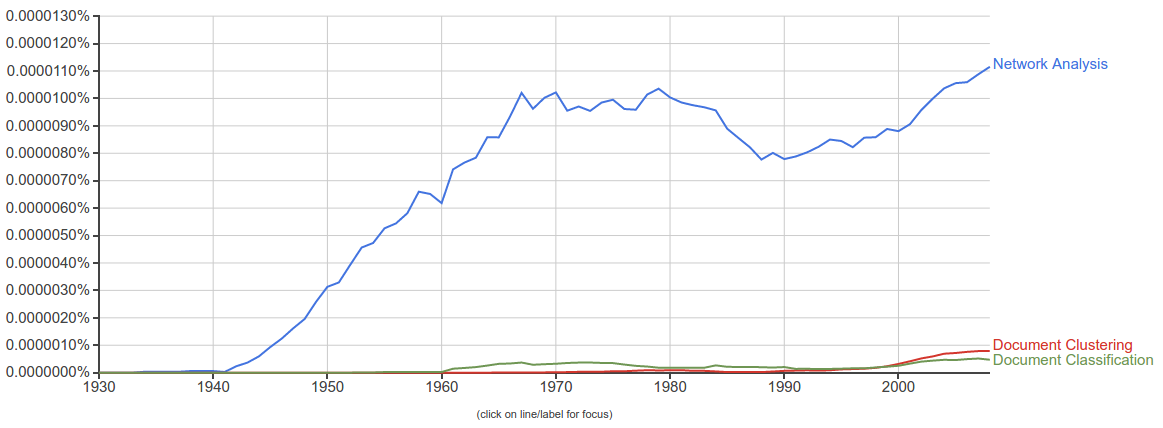
\includegraphics[width=13.7cm]{ngram-viewer/ngram_viewer}}
    \caption[Frequencies of the four research topics discussed found in materials printed between 1930 and 2008 within Google's text corpus.]{Frequencies of the four research topics discussed above found in materials printed between 1930 and 2008 within Google's text corpus. Surprisingly, the search engine was unable to find ngrams for \textit{topic-modelling}.}
    \label{figure:ngram_viewer}
\end{figure}

\iffalse
The Background chapter introduced EPSRC and the problem addressed in this research project while also providing background to several concepts in network science, community detection algorithms and other forms of classification. This section presents the literature reviewed prior to commencing this project identify related works and determine whether studies with a similar focus as this one have already been completed.

\vspace*{1em}

\textbf{Community Structure on Wikipedia} \cite{wikipedia_community_structure} documents community structure thoroughly and provided a good starting point to the literature survey. The article describes the properties and application of community structures in networks. Moreover, it gives a detailed description of a significant number of community detection algorithms as well as several testing methods enabling the evaluation of the algorithms. The information on Wikipedia helped to gain a general understanding of the subject and identify the further direction of the survey.

\vspace*{1em}

\textbf{Community Detection and Mining in Social Media} \cite{community_detection_class} is a class taught by \textit{Lei Tang} (Yahoo! Labs) and \textit{Huan Liu} (Arizona State University) at Arizona State University. The class follows the teachings of a book with the same name \cite{tang2010community} published by \textit{Lei Tang} and \textit{Huan Liu} in 2010. The information from the class is available online in the form of PowerPoint presentations. Essentially, they provide a summary, highlighting the most important parts from the book. The class added the academic knowledge required to the literature survey while also expanding on the information gathered from Wikipedia in regards to community detection evaluation.

\vspace*{1em}

\textbf{Community structure in social and biological networks} \cite{girvan2002community} is a research paper authored by \textit{Michelle Girvan} and \textit{Mark EJ Newman} and published in 2002. The research paper introduces the community structure property, present in many networks. It defines the community structure of a network as network nodes linked together in densely connected clusters, between which there are only sparser connections.

Girvan and Newman also propose a method to detect communities in networks which is built based on the idea of centrality indices. The method is tested on both \textit{real-world} and \textit{computer-generated} networks whose community structure is both known and unknown. \textit{Real-world} networks used for testing include \textit{Zachary's Karate Club Study} and \textit{College Football}. The study used networks without a known community structure such as the \textit{Collaboration} and \textit{Food Web} networks. In the case of a known community structure, the authors found that the method performed well and identified the known community structure with high-sensitivity and reliability. Furthermore, in both cases of unknown community structure, the method still detected significant and informative community divisions.

This research paper was extremely beneficial as it provided further knowledge in the field of community detection as well as the concepts and methods required to complete this research project.

\vspace*{1em}

\textbf{Finding and evaluating community structure in networks}
\cite{newman2004finding} is another paper published in 2004 by \textit{Mark EJ Newman} and \textit{Michelle Girvan} and similar to their previous collaborative work, \textit{Community structure in social and biological networks}. In this publication, the authors propose a set of algorithms for identifying community structure in networks, which is defined as "natural divisions of network nodes into densely connected subgroups." Moreover, this paper represents the introduction of the community structure measure known as \textit{modularity}.

The proposed algorithms include shortest-path betweenness, resistor networks and random walks. A way to measure the strength of the community structure identified by the algorithms proposed is also introduced. The measure provides an objective metric for determining the number of communities a network should be divided into. Testing the algorithms on both \textit{computer-generated} and \textit{real-world networks}, \textit{Newman} and \textit{Girvan} demonstrate that the algorithms are extremely effective at identifying community structure.

The knowledge gained from this study was extremely helpful throughout the duration of this project. It explained how the algorithms proposed were built and how they work, while also providing examples of networks on which the algorithms were evaluated on. It also showed the progress of \textit{Newman} and \textit{Girvan} in the subject since their previous collaborative research effort.

\vspace*{1em}

\textbf{Topic oriented community detection of rating based social networks} is a study conducted by \textit{Reihanian et al.} \cite{reihanian2015topic} in 2015 focusing on community detection from the perspective of content analysis. Most community detection research chooses to focus only on the topological structure of the network. In a social network, for example, this is usually based on the number of communications among individuals. In contrast, this research paper aims to go further and explore and analyse the network's content flow.

The development process of the project commences by preprocessing and annotating topic labels and continues with the clustering of social objects and the creation of topic clusters. It concludes by applying a community detection algorithm to the produced topical clusters in order to identify the community structure within each cluster. Furthermore, a number of experiments are carried out on several data sets including \textit{Movielens 100k}, \textit{Book-Crossing}, \textit{CIAO}, \textit{MovieTweetings} and \textit{Movielens Latest}. It makes use of a performance metric, \textit{purity}, as defined by Zhao et al. \cite{zhao2012topic} which considers both topic and linkage structure. It identifies a maximum \textit{purity} value in each experiment as the topical clusters created in each data set incorporate members which are interested in the same unique topics.

Moreover, the study also compares the topic-oriented community detection proposed with the classical community detection method in which topical content is not analysed. It finds higher values of \textit{modularity} and \textit{purity} in the topic-oriented framework, as the basic network is partitioned into topical clusters, and members who have the same topic of interest are clustered into the same identified community.

\textit{Topic oriented community detection of rating based social networks} has similarities to this project in terms of the focus on topic analysis. It added a new, different perspective to the process of community structure detection which is extremely interesting and definitely a potential path of extending research.

\vspace*{1em}

\textbf{Community detection algorithms: a comparative analysis} is a research paper published by \textit{Lancichinetti et al.} \cite{lancichinetti2009community} in 2009 focusing on the comparison of a wide range of community detection algorithms. Two evaluation benchmarks are employed, the \textit{GN benchmark} by \textit{Girvan} and \textit{Newman} and the \textit{LFR benchmark} proposed by \textit{Lancichinetti et al.}

The community detection algorithms are tested on each evaluation benchmark and include the \textit{Fast greedy modularity optimization}, \textit{Exhaustive modularity optimization via simulated annealing}, \textit{Cfinder},  \textit{Markov Cluster}, \textit{Expectation-maximization} and \textit{Potts model approach}. Furthermore, a number of different graphs were used in the evaluation such as \textit{undirected} and \textit{unweighted} graphs, \textit{directed} and \textit{unweighted} graphs, \textit{undirected} and \textit{weighted} graphs and \textit{undirected} and \textit{unweighted} graphs with overlapping communities. On both evaluation benchmarks, the study found that the \textit{Dynamic algorithm (Infomap)} by \textit{Rosvall} and \textit{Bergstrom} performed the best. The \textit{Fast modularity optimization} by \textit{Blondel et al.} and the \textit{Potts model approach} by \textit{Ronhovde} and \textit{Nussinov} also had a good performance in the evaluation.

This comparative analysis served as a significant source of knowledge in terms of the community detection algorithms available, how they work, when they work best and on which networks. It definitely had an impact on the decisions made in this project in regards to community detection methods utilised. 

\vspace*{1em}

\textbf{On Accuracy of Community Structure Discovery Algorithms} is another comparative study authored by \textit{Orman et al.} \cite{orman2011accuracy} in 2011. It evaluates the majority of algorithms evaluated in \textit{Community detection algorithms: a comparative analysis}, with the exception of \textit{SpinGlass} by \textit{Reichardt} and \textit{Bornholdt} and \textit{Walktrap} by \textit{Pons} and \textit{Latapy}. A generated benchmark graph using the \textit{LFR benchmark} is used. This means that only artificial networks are taken into consideration while the community structure is already known. Each of the eleven community detection algorithms presented are tested on all generated network samples.

The study found that in all cases the \textit{Dynamic algorithm (Infomap)} by \textit{Rosvall} and \textit{Bergstrom} performed better than all other algorithms. \textit{Infomap} succeeded in identifying the communities even for high mixing coefficient values. Furthermore, \textit{Walktrap}, \textit{Markov Cluster}, \textit{Spinglass} and \textit{Louvain} also had an excellent performance level, although not as good as \textit{Infomap}. The research also discovered that for all algorithms, the higher the degree, the better the performance. Moreover, when the network size increases, some algorithms (\textit{Infomap}, \textit{Infomod}, \textit{Louvain}) performed better, others performed worse (\textit{Commfind}, \textit{SpinGlass}, \textit{LeadingEigenvector}, \textit{Radetal}) while the performance of the remaining algorithms (\textit{Walktrap}, \textit{FastGreedy}, \textit{MarkovCluster}) did not change.

This publication served as a reliability test which determined whether the findings in \textit{Community detection algorithms: a comparative analysis} were consistent when compared to other studies. The findings were indeed consistent as both studies identified more or less the same high-performance and low-performance algorithms. This helped to further solidify the decisions taken surrounding community detection algorithms in this thesis project.

\vspace*{1em}

\textbf{Analysis of Citation Networks} is a university project lead by \textit{Anita Valmarska} and \textit{Janez Dem\u{s}ar} at \textit{Jo\v{z}ef Stefan Institute} in \textit{Ljubljana}, \textit{Slovenia}. It focuses on the analysis of citation networks defined as directed networks where one research paper cites another. The data comprises of a collection of 63826 unique psychology-related papers crawled from \textit{Wikipedia} and \textit{Microsoft Academic Research data (MAS)}.

The resulting network consists of 3918 vertices connected by 5732 edges. The study employs the \textit{Louvain} method for the detection of community structure in the created network. The community detection algorithm detected 52 communities with the smallest cluster consisting of 7 research papers, while the largest cluster was constructed of 230 psychology-related publications. The study finds that the results produced have potential as the representation of the communities reveals sensible relationships between psychology sub-fields.

\textit{Analysis of Citation Networks} is the closest in terms of scale to this research project and provides an example of the data, algorithms and tools that other researchers used. Furthermore, it yields new knowledge and inspiration which contributed to the analysis process of this thesis project.
\fi
\chapter{\textsc{Project Design}}
\label{chapter:project_design}

As a result of the project design phase, the problem statement and objectives were established, while the motivation behind the project was defined. A high-level sense of the methodology employed is also presented, together with a flow-chart created during the project planning phase.

\section{Problem statement}

The problem addressed in this project is concerned with the rational clustering of networks constructed using real data. This project focuses on identifying a solution to a real-world problem faced by EPSRC involving the definition of topic classifications. EPSRC is in possession of substantial grant data which can be used to formulate networks of \textit{topics} and \textit{researchers}. Ideally, the next step would involve the division of the networks created in order to obtain several groups of topics based on similarity or relatedness. The "best" group would represent the classification of its topics to a research area. This method would make the finer or coarser definition of topics significantly easier. However, as of yet, a way of achieving this has not been identified.

\section{Objectives and Motivation}

The overall aim of this project can be divided into three different objectives of diverse importance. Firstly, and most importantly, at the end of the project, a rational clustering of topics is expected to be produced using graph theory. Secondly, and equally as important, the project seeks to prove that a novel approach in graph theory can be employed to solve and provide a solution to the real-world problem addressed. Finally, this thesis project also aims to demonstrate that the novel approach can be applied to a different data set involved in the clustering of researchers.

Furthermore, the motivation behind this thesis project is primarily fuelled by the real-world aspect of the problem considered. Personally, I believe that contributing towards something that may be beneficial to other people adds enthusiasm which translates into a more efficient work rate and higher standard of quality.

Originally, the concept of the project came from Dr. Shi Zhou, the supervisor of this thesis project. Recently, he attended a talk where an EPSRC officer expressed concerns regarding the way research topics were defined. Therefore, the project was principally specific to one organisation and problem. However, with time, the data took on a new significance as the invaluable human judgement underlying it was discovered. This changed the aim of the project as it became a project concerned with a general real-world problem. In this new meaning, graph theory combined with the human judgement behind the links connecting the topics in a network is used to identify an optimal way of clustering topics meaningfully. 

\section{Methodology}

This project uses current and historical data publicly provided by EPSRC through the EPSRC Grants on the Web (GoW) service. Networks of \textit{Topics} and \textit{Researchers} are constructed using the data collected from EPSRC. Node and edge attributes are also formulated, and the attribute values normalised. This is followed by extensive comparison experiments on two different interpretations of the two types of networks considering three different edge weight interpretations and eight different community detection algorithms. The three edge weight interpretations are \textit{unweighted}, \textit{weighted by the normalised number of grants} and \textit{weighted by the normalised value of grants}, while community detection algorithms include \textit{Spinglass}, \textit{Louvain} and \textit{Fast Greedy}. Subsequently, the topic and researcher clusters are evaluated by calculating the average Dice and Jaccard similarity of node pairs between and within the clusters. The results of the experiments are expected to represent the identification of an optimal combination of edge weight and community detection algorithm which produces a coherent, balanced and well-defined clustering of topics and researchers.

\clearpage

\section{Project Plan}

Prior to development and analysis stages, a plan was produced in the form of a flow chart, presented in Fig. \ref{fig:flow_chart}, which details every major process that was completed in order to achieve the objectives set in the Project Design.

\begin{figure}[htpb]
    \centering
    \fbox{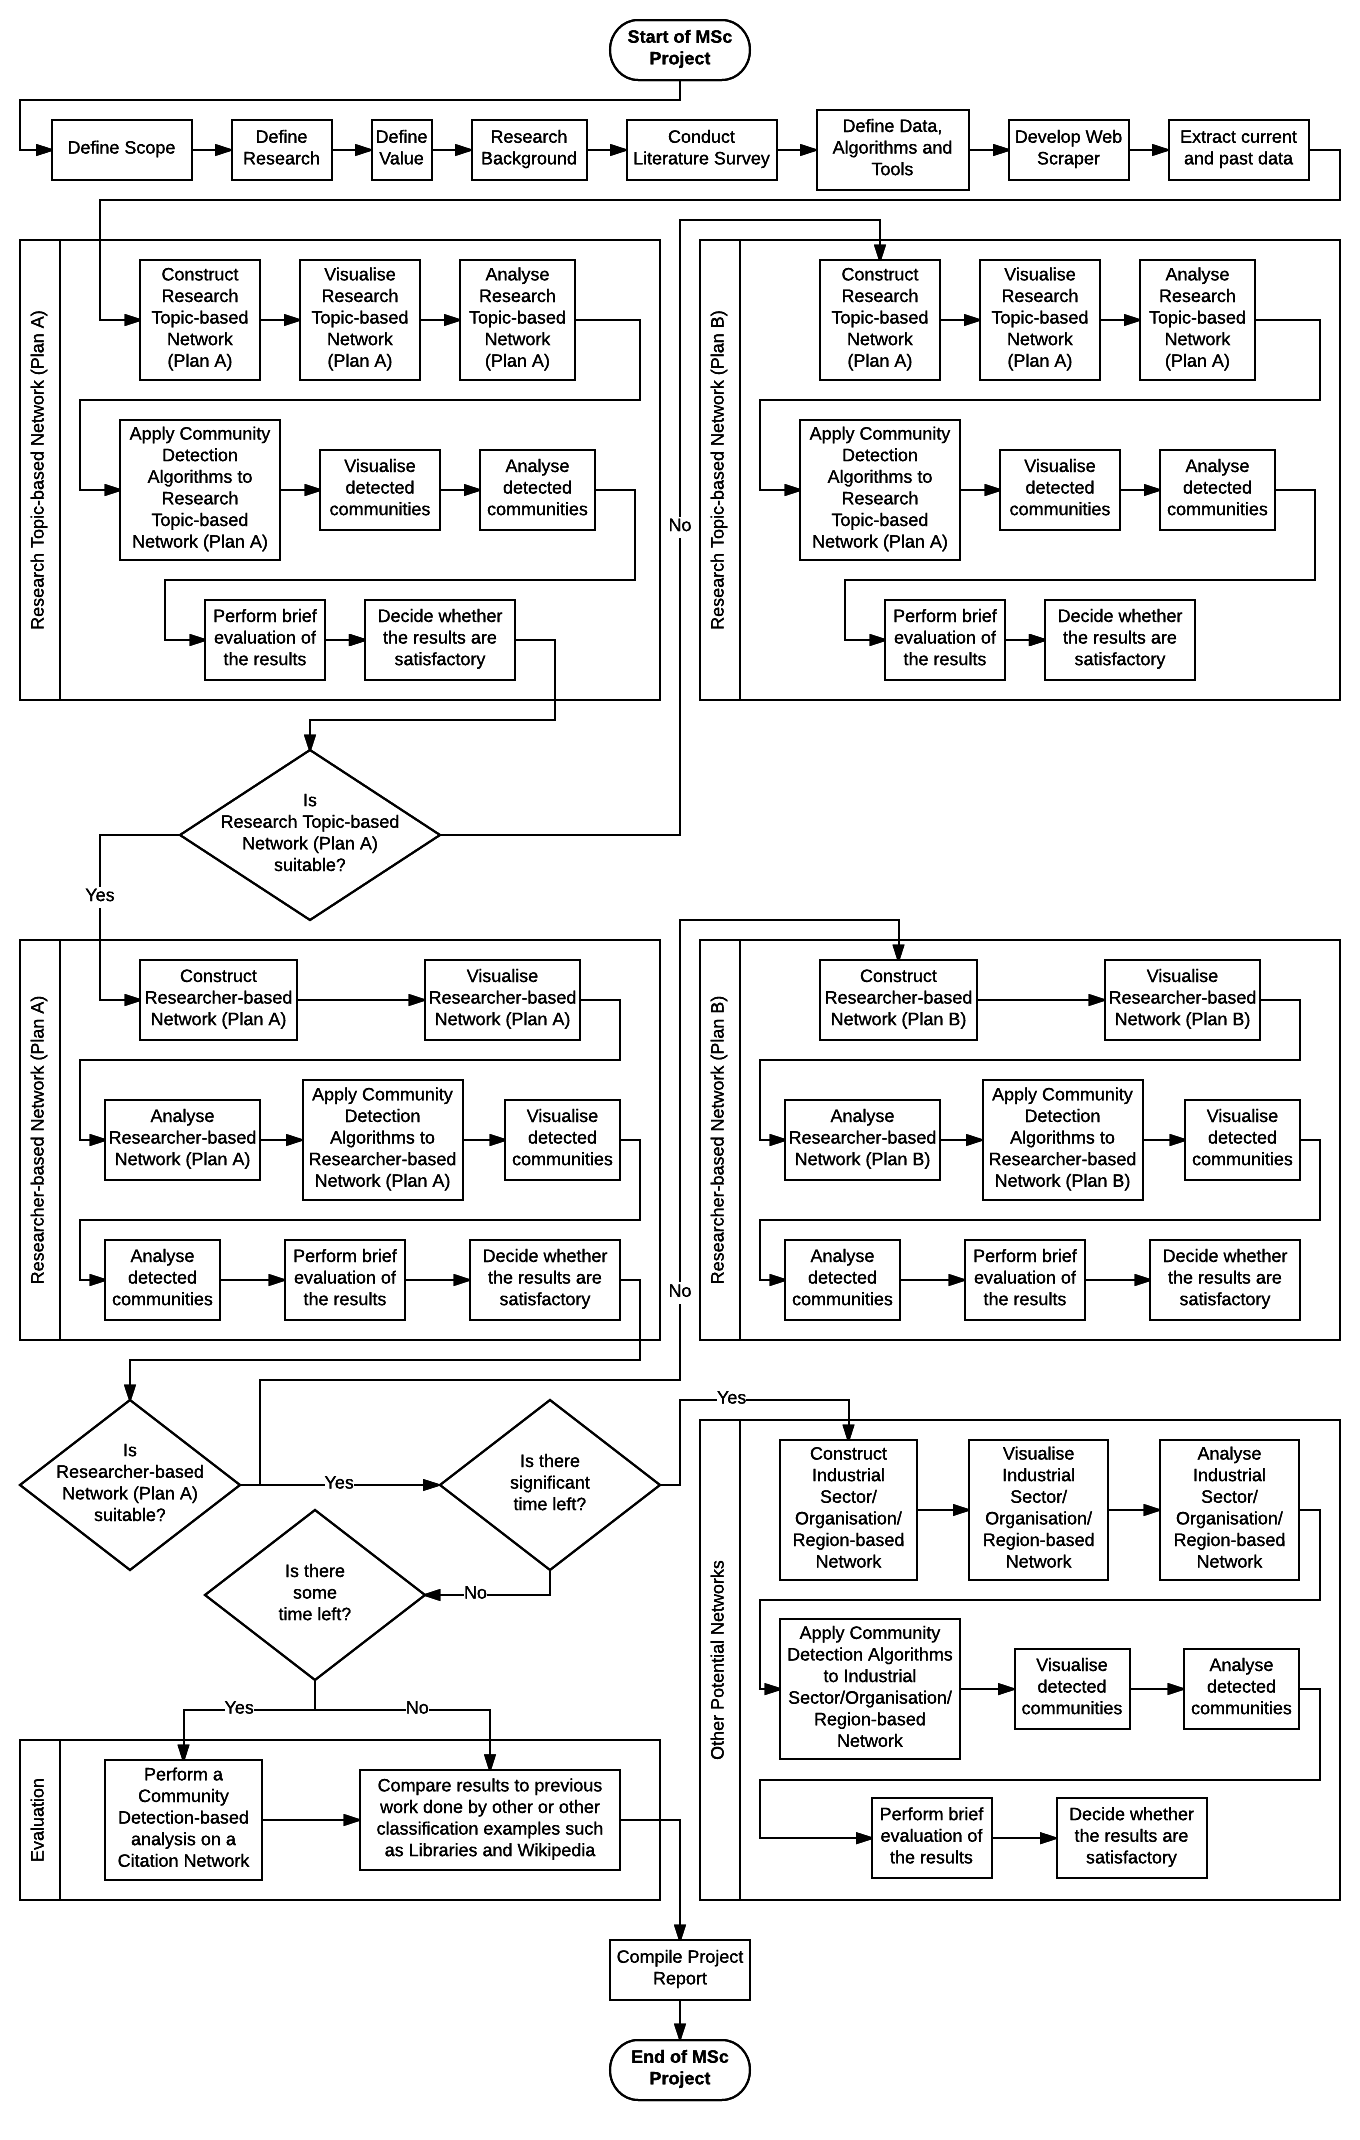
\includegraphics[width=11.5cm]{flow-charts/flow_chart}}
    \caption{Flow chart created as part of the Project Plan, showing the transition between the different stages of the project.}
    \label{fig:flow_chart}
\end{figure}

\clearpage
\chapter{\textsc{Methodology}}
\label{chapter:methodology}

This chapter extends the Methodology section in Chapter \ref{chapter:project_design}: Project Design. Firstly, it provides an introduction to the EPSRC grant data used in this project and details its collection process. Secondly, the networks generated from the collected EPSRC data are introduced. Thirdly, the tools used in this project are presented and their use is highlighted. Furthermore, the contrast between grants as edges and grant records is outlined. Additionally, the process of formulating the node and edge attributes is presented, together with the normalisation process of the attribute values. Finally, the common experiment settings employed in all experiments are specified and the experiment process in which several edge weight interpretations and community detection algorithms are interchangeably tested is briefly described.

\section{EPSRC grant data}

This project uses data provided publicly by EPSRC through the \textit{EPSRC GoW} service. It consists of current and historical data stored within the \textit{Current} and \textit{Past Grant Portfolio}, respectively.

\subsection{EPSRC GoW service}

The \textit{GoW} service is a web-based facility providing information about research grants funded by EPSRC. The service is updated frequently, and consists of large amounts of information regarding historical and current grants, researchers, panels and quarterly summaries. It also includes search functionality allowing users to search the Web database.

\subsection{EPSRC Current and Past Grant Portfolio}

The \textit{Current} and \textit{Past Grant Portfolio} are sub-facilities of the \textit{GoW} service providing access to current and historical grant data. Both facilities provide the same kind of information, however the access to information differs slightly. The \textit{Past Grant Portfolio} requires a time period to be supplied, and provides grants based on it. This can be a start date, an end date or a start and end date. Fig. \ref{fig:current_grant_portfolio} and Fig. \ref{fig:past_grant_portfolio} present the hierarchical structure of the EPSRC \textit{Current} and \textit{Past Grant Portfolio}, respectively.

\begin{figure}[htpb]
    \centering
    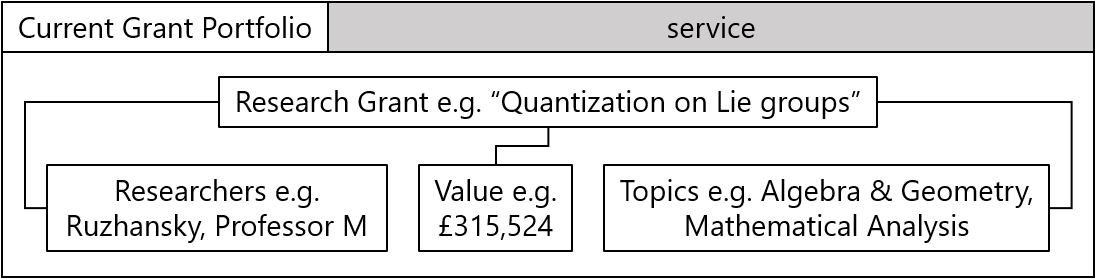
\includegraphics[width=10cm]{portfolios-explained/current_grant_portfolio}
    \caption{Hierarchical structure of the EPSRC Current Grant Portfolio.}
    \label{fig:current_grant_portfolio}
\end{figure}

\begin{figure}[htpb]
    \centering
    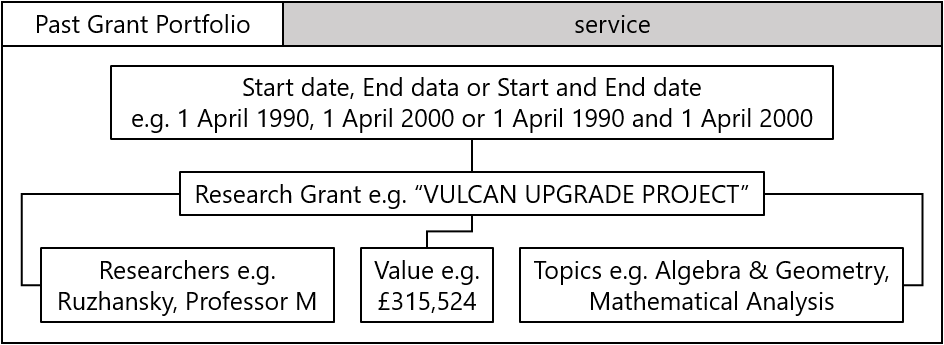
\includegraphics[width=10cm]{portfolios-explained/past_grant_portfolio}
    \caption{Hierarchical Structure of the EPSRC Past Grant Portfolio.}
    \label{fig:past_grant_portfolio}
\end{figure}

Each grant record is stored within a separate web page and contains details about the grant such as \textit{reference}, \textit{investigators (researchers)}, \textit{partners}, \textit{department}, \textit{organisation}, \textit{start} and \textit{end date}, \textit{value} and \textit{topic} and \textit{industrial sector classifications}. Fig. \ref{fig:grant_record} shows an example of a grant record within the \textit{EPSRC GoW} service.

\begin{figure}[htpb]
    \centering
    \fbox{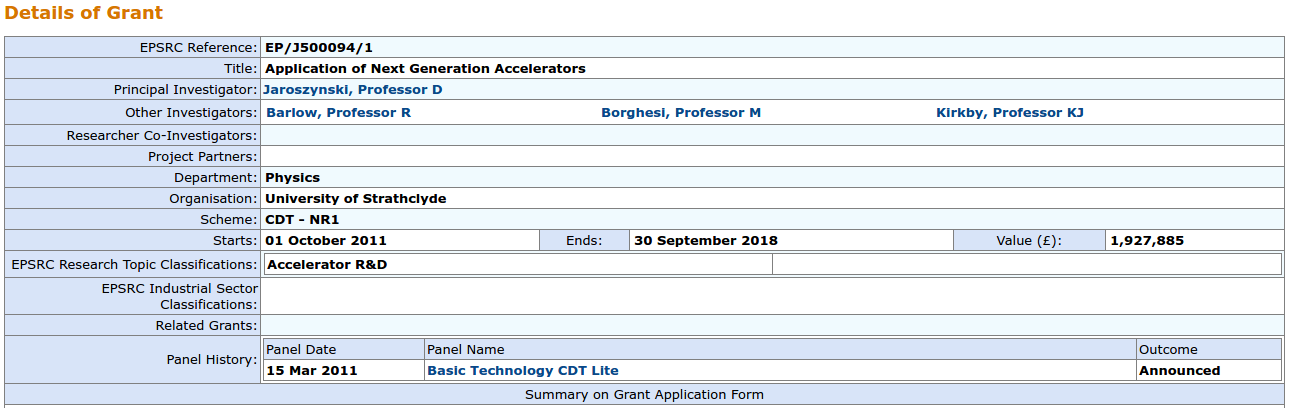
\includegraphics[width=12cm]{epsrc-records/grant_record}}
    \caption{Grant record in the \textit{EPSRC GoW} service.}
    \label{fig:grant_record}
\end{figure}

The researchers within each grant record are linked to separate researcher records. Each researcher record is also stored within a separate web page and contains details about the researcher including \textit{name}, \textit{organisation}, \textit{department}, \textit{current topics} and \textit{grants}. Fig. \ref{fig:researcher_record} shows an example of a researcher record within the \textit{EPSRC GoW} service.

\begin{figure}[htpb]
    \centering
    \fbox{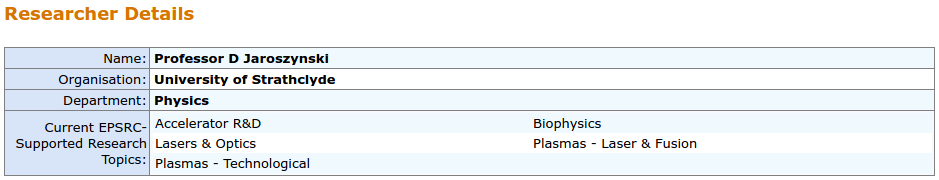
\includegraphics[width=12cm]{epsrc-records/researcher_record}}
    \caption{Researcher record in the \textit{EPSRC Grants on Web (GoW)} service.}
    \label{fig:researcher_record}
\end{figure}

\section{Collection of data from EPSRC}

The previous sections provided an introduction to the data provided by EPSRC, the \textit{Grants on the Web service (GoW)}, the \textit{Current} and \textit{Past Grant Portfolios} and the \textit{Grant} and \textit{Researcher} records. This project solely uses data collected from the \textit{Current} and \textit{Past Grant Portfolios}, and does not use any of the other information provided through the \textit{GoW} service. In terms of the \textit{Current} and \textit{Past Grant Portfolios}, this project only makes use of data extracted from grant and researcher records. 

Firstly, data within the following fields of a grant record was extracted:
\textit{EPSRC Reference}, \textit{Principal Investigator}, \textit{Other Investigators}, \textit{Starts}, \textit{Ends} and \textit{EPSRC Research Topic Classifications}. Secondly, data within the \textit{Name} and \textit{Current EPSRC-Supported Research Topics} fields of a researcher record was extracted.  Table \ref{table:grant_researcher_record_numbers} presents the number of current and historical EPSRC grant and researcher records from which data was collected.

\begin{table}[!htbp]
\renewcommand*{\arraystretch}{1.4}
\centering
\caption{Number of current EPSRC grant and researcher records and historical grant records from which data was collected.}
\label{table:grant_researcher_record_numbers}
\begin{tabular}{r|r|r|r}
{} & \multirow{2}{*}{\textbf{Current}}
& \multicolumn{2}{c}{\textbf{Historical}}\\
\cline{3-4}
& {} & \textbf{1990-2000} & \textbf{2000-2010}\\
\hline
\textbf{Number of Grant records}      & {3175} & {17861} & {18692}\\
\textbf{Number of Researcher records} & {5874} & {10820} & {13385}\\
\end{tabular}
\end{table}

\clearpage

\noindent Furthermore, the current and historical data used in this project is organised into two main data sets, while the historical data set is further divided into two sub-data sets as follows:

\begin{itemize}[noitemsep]
    \item \textbf{Current data set}, consisting of current (post 2010 start date) grant records collected on 8 July 2016 
    \item \textbf{Historical data set}, consisting of grant records from two time periods:
    \begin{itemize}
        \item \textbf{1990 to 2000}, consisting of grant records which started and ended between 1 April 1990 and 1 April 2000
        \item \textbf{2000 to 2010}, consisting of grant records which started and ended between 1 April 2000 and 1 April 2010
    \end{itemize}
\end{itemize}

As previously mentioned, both grant and researcher records are stored as separate web pages within the \textit{GoW} service. In order to extract content from a web page, a technique called \textit{web scraping} is employed. This is usually achieved by either using a third-party web scraper or by developing a web scraper from scratch, which extracts specified data from the underlying tags within the HTML code. In this case, a web scraper was developed using the \textit{requests} and \textit{lxml} Python libraries.

Essentially, the web scraper connects to the URL of each grant and researcher record and extracts the text found under specific fields such as \textit{Reference}, \textit{Principal Investigator} and \textit{Other Investigators}, \textit{Value} and \textit{EPSRC Research Topic Classifications}. Once extracted, the data is validated and then comma-delimited and text qualified using quotation marks which preserves its original format and allows easy manipulation of it. Subsequently, it is stored within comma-separated files categorised by content and data set.

\clearpage

\section{Generation of networks from EPSRC data}

The data extracted from the \textit{GoW} service was used to construct several networks of topics and researchers structured as follows:

\begin{enumerate}[noitemsep, label*=\arabic*.]
    \item \textbf{Networks of Topics, with nodes representing \underline{topics}}
    \begin{enumerate}[label*=\arabic*.]
        \item \textbf{Topic-grant network}, with edges representing \underline{grants};
            \begin{enumerate}[label*=\arabic*.]
                \item current version using the current data set (2010-2016)
                \item historical version using historical data set (2000-2010)
                \item historical version using historical data set (1990-2000)
            \end{enumerate}
        \item \textbf{Topic-researcher network}, with edges representing \underline{researchers};
            \begin{enumerate}[label*=\arabic*.]
                \item current version using the current data set (2010-2016)\footnote{The Topic (Nodes as Topics, Edges as Researchers) and Researcher network (Nodes as Researchers, Edges as Topics) were created using the Current data set only because Researcher records only consist of a researcher's current topics, and not their historical topics.}
            \end{enumerate}
    \end{enumerate}

    \item \textbf{Networks of Researchers, with nodes representing \underline{researchers}}
    \begin{enumerate}[label*=\arabic*.]
        \item \textbf{Researcher-grant network}, with edges representing \underline{grants};
        \begin{enumerate}[label*=\arabic*.]
                \item current version using the current data set (2010-2016)
                \item historical version using historical data set (2000-2010)
                \item historical version using historical data set (1990-2000)
            \end{enumerate}
        \item \textbf{Researcher-topic network}, with edges representing \underline{topics};
        \begin{enumerate}[label*=\arabic*.]
                \item current version using the current data set (2010-2016)\footnotemark[1]
        \end{enumerate}
    \end{enumerate}
\end{enumerate}

\section{Tools used in this project}

During this study, several tools were employed in order to accomplish various development and analysis activities. This section describes the tools and comments on their use throughout the project.

\subsection{JetBrains PyCharm for programming}

JetBrains PyCharm \cite{jetbrains_pycharm} is an Integrated Development Environment (IDE) for programming in Python. It also provides support for writing code in Bash. It was used to write the development code in primarily Python but also in Bash.

\subsection{Microsoft Excel for data storage}

Microsoft Excel \cite{microsoft_excel} is a spreadsheet software featuring calculation, graphing tools, pivot tables, and macro programming support in Visual Basic. It was used to explore, filter and validate the collected data.

\subsection{iGraph for network analysis and visualisation}

iGraph \cite{csardi2006igraph} is a library collection for creating and manipulating graphs and analyzing networks. This tool was used to compute network properties, apply community detection algorithms, and produce visualisations of the networks created.

\subsection{NetworkX for visualising adjacency matrices}

NetworkX \cite{networkx} is a package for the creation, manipulation, and study of the structure, dynamics and functions of complex networks in Python. It was used to visualise adjacency matrices.

\subsection{Wordle for creating word cloud visualisations}

Wordle \cite{wordle} is a tool for visualising text as word clouds. By default, it computes each word's frequency and displays the more frequent words in a larger font than less frequent ones. Additionally, Wordle's advanced mode allows keeping words together, specifying a weight which controls the font size, as well as specifying a colour for each word. It was to create word cloud representations of topic clusters using several attributes to control font size and colour.

\subsection{Adobe Photoshop for image editing}

Adobe Photoshop \cite{adobe_photoshop} is a graphics editor developed by Adobe Systems. It was used for image editing as well as turning network plots produced using iGraph into complete network visualisations.

\section{Common tasks}

A number of tasks were carried out for every network constructed using every data set, therefore, the tasks are considered common and are described in this section. They include identifying the contrast between grants as edges and grant record, the formulation of node and edge attributes and the normalisation of attribute values.

\subsection{Contrast between grants as edges and grant records}

It is essential to point out that there is a clear difference between grants represented by edges and the actual grant records that appear on the \textit{GoW} service. First and foremost, the former is not unique within a network, while the latter is unique within the \textit{GoW} service. This is due to the way links between topics or researchers were established in a network. If a pair of topics co-appear in X grants, the two will in theory be linked by M edges. In this study, the M edges are merged into a single edge between the two topics, and the weight of the edge is assigned as the total sum of the X grants. Essentially, if a grant is associated with N topics, N(N-1)/2 edges are created to link the N topics into a fully connected mesh graph. For example, if grant Y has 4 topics, 6 edges are created linking the topics into a 4-clique graph. Furthermore, it is also crucial to specify that unlike grants, a network consists of nodes representing unique topics.

This causes issues when questions like the following are posed: \textit{How many grants are in a specific community within a network's community structure?} \textit{What is the value of the grants?} It is important to mention that it is not known which grant is represented by an edge. It is only known that it represents one or more grants depending on the edge weight. If this was known, providing an answer to the above questions becomes significantly easier. In contrast, the answer was achieved through a lengthier process. Furthermore, the edges linking topics within the same community and the edges linking topics from different communities were known. This greatly aided the identification process of both the number and value of grants within communities and between communities.

Firstly, the origin and destination topics of an edge within a network were retrieved. Secondly, during the data collection process, a data structure was created which stored the reference of each grant record and the topics that classify it. Next, a check was carried out against all grant records which verified whether both the retrieved origin and destination topics appeared under a grant record. Number and value counters were created to keep track of the cumulative number and value of grants. If the check was true, the reference and value of the grant were added as the key and value to a Python dictionary, in which all keys must be unique. Finally, at the end of the check, the number of grant references was counted and the grant values were summed up. This provided an answer to the questions asked, as the number and value of grants within a community was successfully identified. Additionally, using the same technique, the computation of the number and value of grants between communities and within the entire network was also achieved. The function written in order to achieve this task is presented in Code snippet \ref{listing:turn_edges_into_grants}, part of Appendix \ref{appendix:code}.

\subsection{Formulation of node and edge attributes}

Every network constructed using the data collected from EPSRC consists of at least one node and edge attribute, while others consist of two attributes. Both \textit{Topic-grant} and \textit{Researcher-grant} networks consist of a \textit{number} and \textit{value} attribute, while the \textit{Topic-researcher} and \textit{Researcher-topic} networks only consist of a \textit{number} attribute. Visually, the network attributes control both the size of the node circle and the thickness of the edge line.

\subsubsection{Number of grants/topics/researchers}

The number attribute has a number of different contexts, depending on the network. Firstly, in the \textit{Topic-grant} and \textit{Researcher-grant} networks, the node number attribute represents the number of grants that a topic or researcher appears in. In the same networks, the edge number attribute represents the number of grants two topics or researchers have in common, meaning they both appear within the same grant record. Secondly, in the \textit{Topic-researcher} network, the node number attribute represents the number of researchers that a topic appears within, while the edge number attribute represents the number of researchers two topics have in common, meaning they both appear within the same researcher record. Thirdly, in the \textit{Researcher-topic} network, the node number attribute represents the number of topics a researcher currently has, while the edge number attribute represents the number of topics two researchers have in common.

\subsubsection{Value of grants}

Similarly, the value attribute also has a number of different contexts, depending on the network. Firstly, networks that are not based on grant data do not contain of the value attribute. Secondly, in the \textit{Topic-grant} and \textit{Researcher-grant} networks, the node value attribute represents the value of a topic or researcher. This represents the value of the grants that contain that specific topic or researcher. In the same network, the edge value attribute represents the value of the grants that two topics or researcher have in common, meaning they both appear within the same grant record.

\subsection{Normalisation of node and edge attribute values}

The numerical values used as the node and edge attributes, especially the value attribute, represent significantly large numbers which cause issues in terms of development, analysis and visualisation. To accommodate this, the values underwent a normalisation process which scaled the value range down. 
The function written in order to achieve this task can be viewed in Code snippet \ref{listing:norm_vals}, part of Appendix \ref{appendix:code}.

\clearpage

\noindent Furthermore, the formula used to normalize the values is presented below:

\begin{equation}
    (val - old\_min) \times new\_range / old\_range) + new\_min)
\end{equation}
where:
\begin{itemize}[noitemsep]
    \item \textit{val} is the value being normalised
    \item \textit{old\_min} is the minimum of the initial value range
    \item \textit{new\_range} is the new range values will be normalised to
    \item \textit{old\_max} is the maximum of the initial value range
    \item \textit{new\_min} is the minimum of the new value range
\end{itemize}

\section{Common experiments settings}

Extensive comparison experiments were conducted with the purpose of identifying an optimal solution for the data used in this project. An optimal solution is represented by a combination of an edge weight interpretation and a community detection algorithm. All candidates were tested on all networks, interchangeably. This means that each community detection algorithm was applied to each network constructed using each edge weight interpretation. The testing criteria is initially based on modularity score and community size. Later, the actual clusters are manually evaluated based on coherence and balance. In total, three different edge weight interpretations and eight different community detection algorithms are considered.

\subsection{Edge weight interpretations}

Previously, the process carried out to normalise the values used as node and edge attributes was described. Depending on the network tested, one or both edge attributes formulated are used in the experiments. Three edge weight candidates are considered as follows:

\begin{enumerate}[noitemsep]
    \item edge weight, interpreted as \underline{\textbf{unweighted}}
    \item edge weight, interpreted as \underline{\textbf{the normalised number of grants}}
    \item edge weight, interpreted as \underline{\textbf{the normalised value of grants}}
\end{enumerate}

\noindent \textbf{Note}: the edge weight candidates may be occasionally abbreviated as \textbf{uw}, \textbf{wnn} and \textbf{wnv}, throughout this report.

Network that are not grant-based such as the \textit{Topic-researcher} and \textit{Researcher-topic} networks only consist of the number attribute, therefore, the experiments on those networks only involve the first two edge weight candidates. Furthermore, the edge weight attribute plays an important role in the clustering performance of the community detection algorithms, which is the reason why it is essential to conduct an experiment considering different edge weights in order to identify an optimal one for the data in question.

\subsection{Community detection algorithms}

In the Background chapter, the notion and multitude of community detection algorithms was introduced. In this project, eight different community detection algorithms are considered as candidates in the experiments:

\begin{enumerate}[noitemsep]
    \item \textbf{Infomap} by Rosvall and Bergstrom
    \item \textbf{Spinglass} by Reichardt and Bornholdt
    \item \textbf{Louvain} by Blondel et al.
    \item \textbf{Label Propagation} by Raghavan et al.
    \item \textbf{Leading Eigenvector} by Newman
    \item \textbf{Walktrap} by Pons and Latapy
    \item \textbf{Fast Greedy} by Newman et al.
    \item \textbf{Edge Betweenness}
\end{enumerate}

Each algorithm has already been tested by its authors and others on several real and artificial networks. In another project, this would make the experiments unnecessary. However, neither algorithm has been applied on the EPSRC data used in this project. Therefore, it is crucial to compare the performance of each algorithm in order to prove its suitability for the EPSRC current and historical data sets.

\subsubsection{Spinglass by Reichardt and Bornholdt}

\textit{Spinglass} is another modularity optimisation proposed by \textit{Reichardt and Bornholdt} \cite{reichardt2006statistical} which is based on a combination between a popular statistical mechanic model called Potts spin glass, and the network community structure. The algorithm applies the technique of simulated annealing on Potts in order to achieve an optimal modularity \cite{orman2011accuracy}.

\subsubsection{Louvain by Blondel et al.}

\textit{Louvain} is a modularity optimisation algorithm introduced by \textit{Blondel et al.} \cite{blondel2008fast}. It proposes a two-phase hierarchical agglomerative approach which is an improvement of Fast Greedy by Newman et al. \cite{newman2004fast} The first phase of the algorithm involves the application of a greedy optimisation in order to detect communities. In the second phase, a new network is constructed using the communities found during the first phase as nodes. Edges between communities are represented as self-loops, while edges within communities are summed and represented as edges between the new nodes. This process is repeated until a single community remains \cite{orman2011accuracy}.

\subsubsection{Fast Greedy by Newman et al.}

\textit{FastGreedy}, an algorithm developed by \textit{Newman et al.} \cite{newman2004fast} is based on a greedy optimisation method also applied to a hierarchical agglomerative approach. Initially, each node represents its own community. The communities are merged by the algorithm step by step until only one remains, containing all nodes. The greedy approach is applied at each step, by considering the largest increase or smallest decrease in modularity as the criteria for merging. Due to the hierarchical nature of the algorithm, it produces a hierarchy of community structures, and the comparison of modularity values determines the best community structure \cite{orman2011accuracy}.
\chapter{\textsc{Networks of Topics}}
\label{chapter:networks_of_topics}

The idea behind a network of topics involves two ways that the network can be constructed. Likewise, the topics within a network can be analysed from the perspective of grants as well as researchers. Technically speaking, nodes in the network will represent topics regardless of perspective. However, edges can represent either grants or researchers. In the end, two different networks of topics are constructed, the \textit{Topic-grant} network and the \textit{Topic-researcher} network.

\section{Topic-grant network}

The \textit{Topic-grant} network consists of nodes representing topics and edges representing grants. The \textit{EPSRC Research Topic Classifications} field in each grant record consists of one or more topics that classify the grant. Only grant records with two or more topics were included in the analysis. Subsequently, a link between each topic and all other topics within each grant record was established. The link signifies the grant record that the topics all have in common, and is represented as an edge in a network. Fig. \ref{figure:topic_a_structure} provides a visual explanation of how the \textit{Topic-grant} network was constructed using the collected EPSRC data, including the formulated node and edge attributes.

\begin{figure}[!htbp]
    \centering
    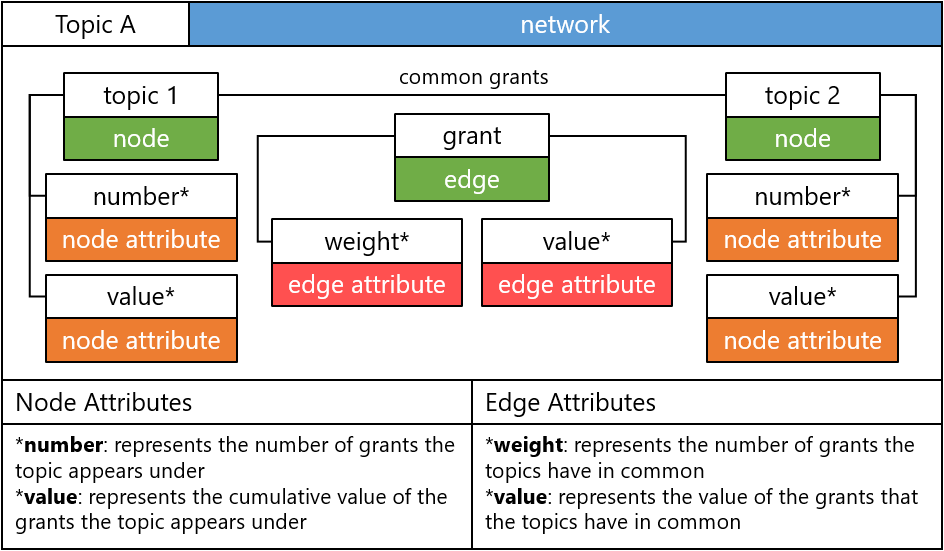
\includegraphics[width=10cm]{networks-explained/topic_network_a}
    \caption[Visual explanation of how the \textit{Topic-grant} network was structured and constructed using the collected EPSRC data]{Visual explanation of how the \textit{Topic-grant} network was structured and constructed using the collected EPSRC data, including the formulated node and edge attributes.}
    \label{figure:topic_a_structure}
\end{figure}

\subsection{Node and edge attributes}

The \textit{Topic-grant} network contains two different node and edge attributes, the number and value of grants. Node and edge attributes are common between networks. Consequently, their formulation is considered a common task, and therefore it is described in Chapter \ref{chapter:methodology}: Methodology.

\subsection{Properties of the Topic-grant network}

The \textit{Topic-grant} network constructed using the current (2010-2016) data set consists of 223 nodes representing as many topics and 2,008 edges representing common grants between topics. Table \ref{table:topic_a_properties} presents the properties of both the historical and current \textit{Topic-grant} networks.

\begin{table}[!htbp]
\centering
\caption[Properties of the \textit{Topic-grant} network constructed using both the historical (1990 to 2000, 2000 to 2010) and current (2010 to 2016) data sets]{Properties of the \textit{Topic-grant} network constructed using both the historical (1990 to 2010, 2000 to 2010) and current (2010 to 2016) data sets.}
\label{table:topic_a_properties}
\begin{tabular}{r|rrr}
{} & \textbf{1990-2000} & \textbf{2000-2010} & \textbf{2010-2016}\\
\hline\\
\textbf{Nodes}                          & {136}     & {208}     & {223}\\
\textbf{Edges}                          & {748}     & {3592}    & {2008}\\
\textbf{Type}                           & {Undirected} & {Undirected} & {Undirected}\\
\textbf{Weighted}                       & {Yes}     & {Yes}     & {Yes}\\
%\textbf{Connected}                     & {Yes}     & {No}      & {Yes}\\
\textbf{Average Degree}                 & {11}      & {34.538}  & {18.009}\\
\textbf{Average Weighted Degree}        & {12.721}  & {35.337}  & {19.543}\\
\textbf{Diameter}                       & {6}       & {5}       & {5}\\
%\textbf{Radius}                        & {3}       & {1}       & {3}\\
\textbf{Density}                        & {0.081}   & {0.167}   & {0.081}\\
\textbf{Modularity}                     & {0.4}     & {0.271}   & {0.373}\\
%\textbf{Communities}                   & {5}       & {5}       & {6}\\
%\textbf{Weak Components}                & {1}       & {2}       & {1}\\
%\textbf{Node Closeness}                & {0.392}   & {0.245}   & {0.423}\\
%\textbf{Node Betweenness}              & {108.536} & {109.776} & {156.483}\\
%\textbf{Edge Betweenness}              & {32.007}  & {12.235}  & {29.706}\\
\textbf{Average Clustering Coefficient} & {0.453}   & {0.59}    & {0.597}\\
%\textbf{Eigenvector Centrality}        & {0.105}   & {0.232}   & {0.204}\\
\textbf{Average Path Length}            & {2.54}    & {2.077}   & {2.395}\\
\end{tabular}
\end{table}

In comparison, both historical networks contain less nodes, with the \textit{2000 to 2010} and \textit{1990 to 2010} networks consisting of 208 and 136 nodes, respectively. This is expected, as the number of research topics in the past was lower, and gradually increased over time. Interestingly, the \textit{2000 to 2010} network consists of more edges which means more topics are connected through common grants. However, the increased number of edges also seems to correlate with the fact that the network is unconnected, while the other networks are connected. A network is unconnected when an edge does not exist between every pair of nodes. Furthermore, all three networks are weighted and in the creation of Table \ref{table:topic_a_properties} and Fig. \ref{figure:topic_a_current_vis}, the number of grants edge weight attribute is used.

\subsection{Visualisation of Topic-grant network}

A visualisation of the \textit{Topic-grant} network, presented in Fig. \ref{figure:topic_a_current_vis}, was produced using iGraph. It features nodes in blue, and edges in grey. The size of the node circle represents the number of grants node attribute. The width of the edge line represents the number of grants edge attribute. The topic(s) that appear in the highest number of grant records are coloured in red.

\begin{figure}[htpb]
    \centering
    \fbox{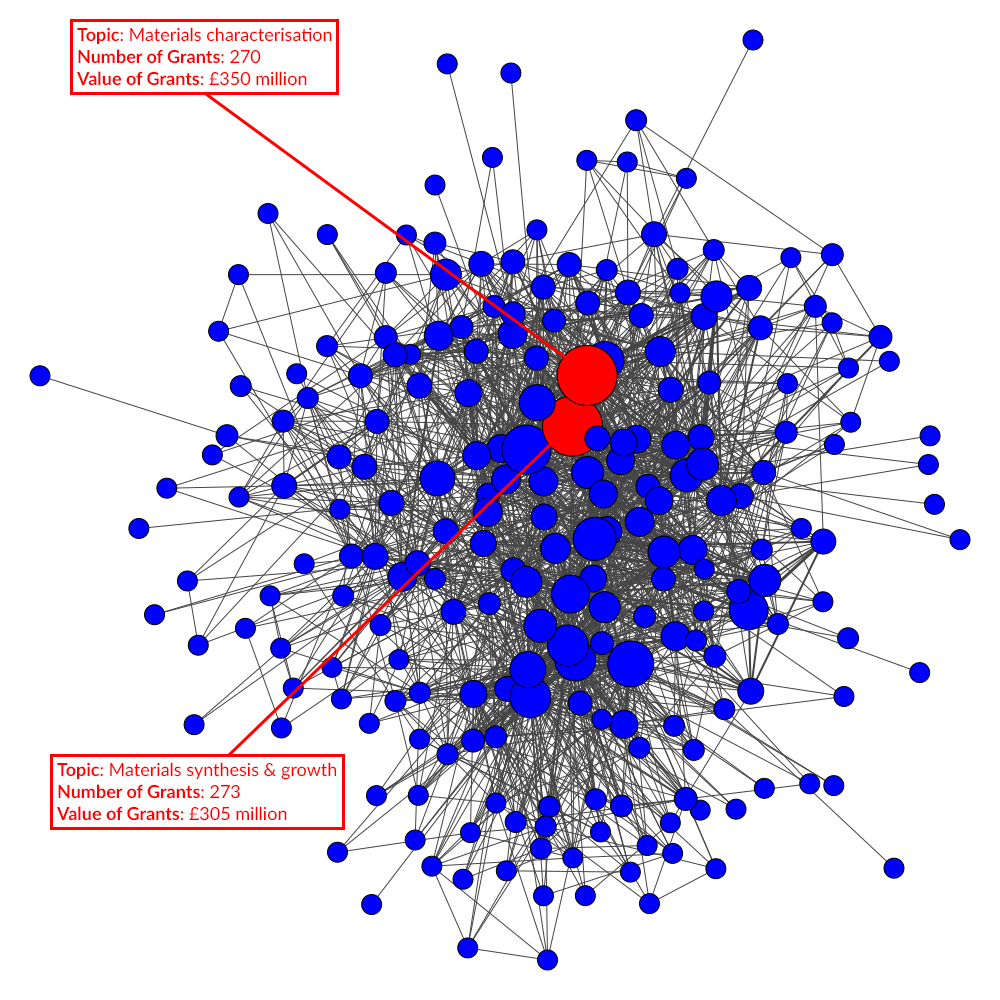
\includegraphics[width=13cm]{networks/topic_a}}
    \caption[Visualisation of \textit{Topic-grant} network constructed using the current (2010 to 2016) data set]{Visualisation of \textit{Topic-grant} network constructed using the current (2010 to 2016) data set. The topic(s) that appear in the highest number of grant records are coloured in red.}
    \label{figure:topic_a_current_vis}
\end{figure}

\section{Topic-researcher network}

The \textit{Topic-researcher} network consists of nodes representing topics and edges representing researchers. The \textit{Current EPSRC-Supported Research Topics} field in each researcher record consists of one or more topics that classify the grants supported by EPSRC that the researcher is currently an investigator in. Only researcher records with two or more topics were included in the analysis. Subsequently, a link between each topic and all other topics within each researcher record was established. The link signifies the researcher record that the topics all have in common, and is represented as an edge in a network. Fig. \ref{figure:topic_b_structure} provides a visual explanation of how the \textit{Topic-researcher} network was constructed using the collected EPSRC data, including the formulated node and edge attributes.

\begin{figure}[!htbp]
    \centering
    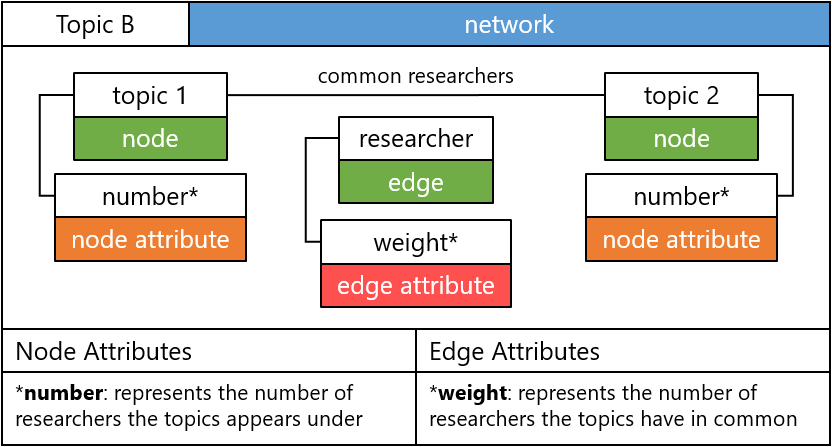
\includegraphics[width=10cm]{networks-explained/topic_network_b}
    \caption[Visual explanation of how the \textit{Topic-researcher} network was structured and constructed using the collected EPSRC data]{Visual explanation of how the \textit{Topic-researcher} network was structured and constructed using the collected EPSRC data, including the formulated node and edge attributes.}
    \label{figure:topic_b_structure}
\end{figure}

\subsection{Node and edge attributes}

The \textit{Topic-researcher} network contains one node and edge attribute, the number of grants. In the \textit{Topic-researcher network} edges represent researchers, therefore, it does not contain the value of grants attribute. Node and edge attributes are common between networks. Consequently, their formulation is considered a common task, and therefore it is described in Chapter \ref{chapter:methodology}: Methodology.

\subsection{Properties of Topic-researcher network}

The \textit{Topic-researcher} network represents the second interpretation of the topic data, and consists of topics represented by 225 nodes connected by 5,192 edges. Table \ref{table:topic_b_properties} presents the properties of the \textit{Topic-researcher} network.

\begin{table}[!htbp]
\centering
\caption[Properties of the \textit{Topic-researcher} network constructed using the current (2010 to 2016) data set]{Properties of the \textit{Topic-researcher} network constructed using the current (2010 to 2016) data set.}
\label{table:topic_b_properties}
\begin{tabular}{r|r}
{} & \textbf{2010-2016}\\
\hline\\
\textbf{Nodes}                          & {225}\\
\textbf{Edges}                          & {5192}\\
\textbf{Type}                           & {Undirected}\\
\textbf{Weighted}                       & {Yes}\\
%\textbf{Connected}                     & {Yes}\\
\textbf{Average Degree}                 & {46.151}\\
\textbf{Average Weighted Degree}        & {52.436}\\
\textbf{Diameter}                       & {4.0}\\
%\textbf{Radius}                        & {2}\\
\textbf{Density}                        & {0.206}\\
\textbf{Modularity}                     & {0.234}\\
%\textbf{Communities}                   & {4}\\
%\textbf{Weak Components}                & {1}\\
%\textbf{Node Closeness}                & {0.522}\\
%\textbf{Node Betweenness}              & {106.686}\\
%\textbf{Edge Betweenness}              & {9.477}\\
\textbf{Average Clustering Coefficient} & {0.715}\\
%\textbf{Eigenvector Centrality}        & {0.289}\\
\textbf{Average Path Length}            & {1.925}\\
\end{tabular}
\end{table}

There is a substantial increase in the number of edges compared to the \textit{Topic-grant} network. This increase is partly due to the fact that the number of researcher records (5,874) considered in the analysis exceeds the number of grant records (3,175) considered by 2,699 records. Furthermore, this network is also weighted, but this time, the edge weight represents the number of researchers two topics have in common. Moreover, the \textit{Topic-researcher network} was only constructed using the current (2010-2016) data set because researcher records only consist of the current topics of a researcher. This limits the comparison of the \textit{Topic-researcher} and \textit{Topic-grant} networks, as they can only be contrasted based on the current (2010-2016) data set.

Furthermore, it is essential to indicate the slight difference in the number of nodes between the \textit{Topic-grant} network (223 nodes) and \textit{Topic-researcher} network (225 nodes). The former considers grants with two or more topics while the latter considers researchers with two or more topics. In either network, records may exist where a specific topic appears in a single record and is also the single topic within that record. This means that the topic will not be considered in the analysis, as links to other topics cannot be established.

\subsection{Visualisation of Topic-researcher network}

A visualisation of the \textit{Topic-researcher} network, presented in Fig. \ref{figure:topic_b_current_vis}, was produced using iGraph. It features nodes in blue, and edges in grey. The size of the node circle represents the number of researchers node attribute. The width of the edge line represents the number of researchers edge attribute. The topic(s) that appear in the highest number of researcher records are coloured in red.

\begin{figure}[htpb]
    \centering
    \fbox{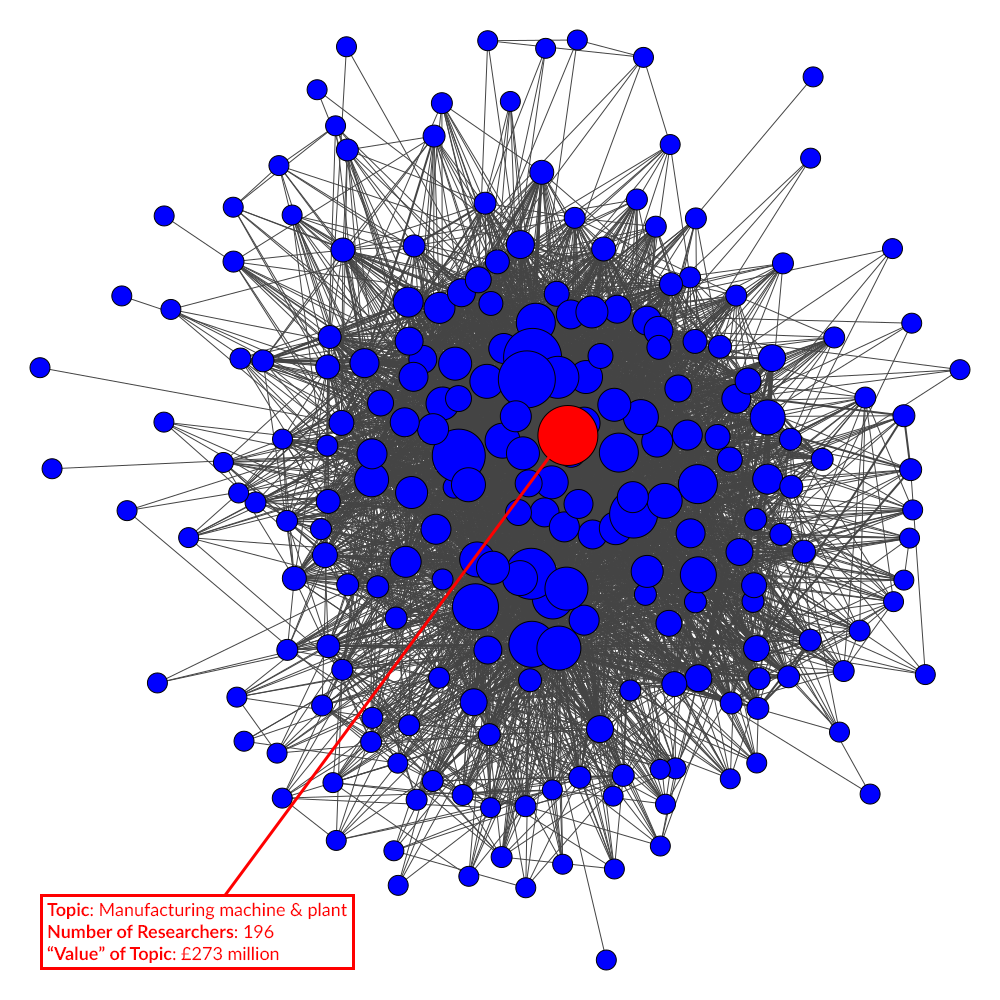
\includegraphics[width=13cm]{networks/topic_b}}
    \caption[Visualisation of \textit{Topic-researcher} network constructed using the current (2010 to 2016) data set]{Visualisation of \textit{Topic-researcher} network constructed using the current (2010 to 2016) data set. The topic(s) that appear in the highest number of researcher records are coloured in red.}
    \label{figure:topic_b_current_vis}
\end{figure}
\chapter{\textsc{Clustering of Topics}}
\label{chapter:clustering_of_topics}

This chapter describes the process of clustering the \textit{Topic-grant} and \textit{Topic-researcher} networks. The experiments carried out are detailed, while the results are presented. Additionally, results are evaluated and discussed through comparisons to historical data and between the two Topic networks.

\section{Clustering of Topic-grant network}

The process of clustering the \textit{Topic-grant} network involves a number of different stages including carrying out experiments, producing results, evaluating results as well as conducting comparative analysis.

\subsection{Experiment}

An experiment was carried out in order to identify an optimal edge weight and community detection algorithm. The full settings of the experiment are outlined and detailed in Chapter \ref{chapter:methodology}: Methodology.

The experiment was divided into a number of phases. In the first phase, a number of community detection algorithms were applied to the current \textit{Topic-grant} network constructed using each of the edge weight. The resulting modularity scores of the identified community structure and the number of generated communities were compared across all edge weight and community detection algorithm candidates. Most community detection algorithms make use of the edge weight attribute in the clustering process, which meant that the \textit{unweighted} edge weight had a low performance and was excluded from the experiment in the first phase. Furthermore, a number of community detection algorithms such as \textit{Label Propagation} and \textit{Edge Betweenness} were also excluded due to low performance. In contrast, the \textit{Louvain}, \textit{Spinglass} and \textit{Fast Greedy} algorithms remained to be tested further in the second phase. Table \ref{table:topic_a_current_modularity} presents the results produced during the first phase of the experiment. The edge weights and community detection algorithms considered for the second phase of the experiment are in \textcolor{red}{\textbf{red}}.

\begin{table}[!htbp]
\centering
\caption[Number of communities and modularity score of the community structure identified in the \textit{Topic-grant} network constructed using the current (2010 to 2016) data set]{Number of communities identified (left value) and the modularity score of the community structure discovered (right value) as a result of applying several community detection algorithms to the \textit{Topic-grant} network constructed using the current (2010 to 2016) data set. Three of the column names are abbreviated: \textbf{uw}, \textbf{wnn} and \textbf{wnv} stand for unweighted, weighted by normalized number of grants and weighted by normalized value of grants, respectively. High-performance candidates are in \textbf{\textcolor{red}{red}}.}
\label{table:topic_a_current_modularity}
\begin{tabular}{r|rrrrrr}
\textbf{} & \multicolumn{2}{c}{\textbf{uw}} & \multicolumn{2}{c}{\textcolor{red}{\textbf{wnn}}} & \multicolumn{2}{c}{\textcolor{red}{\textbf{wnv}}}\\
\hline\\
\textbf{Infomap}             & {3}   & {0.004} & {9}   & {0.332} & {11}  & {0.377}\\
\textcolor{red}{\textbf{Spinglass}} & {6} & {0.355} & {5} & {0.375} & {5} & {0.392}\\
\textcolor{red}{\textbf{Louvain}} & {5} & {0.347} & {6} & {0.373} & {6} & {0.385}\\
\textbf{Label Propagation}   & {1}   & {0.0}   & {1}   & {0.0}   & {1}   & {0.0}\\
\textbf{Leading Eigenvector} & {5}   & {0.312} & {5}   & {0.302} & {10}  & {0.311}\\
\textbf{Walktrap}            & {5}   & {0.279} & {19}  & {0.295} & {24}  & {0.328}\\
\textcolor{red}{\textbf{Fast Greedy}} & {5} & {0.314} & {4} & {0.359} & {5}   & {0.369}\\
\textbf{Edge Betweenness}    & {164} & {0.038} & {166} & {0.042} & {105} & {0.15}
\end{tabular}
\end{table}

During the second phase, the number of topics clustered within each community was compared across all experiment candidates, and it was decided that all remaining edge weights and community detection algorithms should proceed to the final testing phase, in order to be tested further. Table \ref{table:topic_a_current_numbers} presents the results produced in the second phase of the experiment.

\begin{table}[!htbp]
\centering
\caption[Number of topics clustered within each community discovered in the Topic-grant network constructed using the current data set (2010 to 2016)]{Number of topics clustered within each community discovered as a result of applying several community detection algorithms to the Topic-grant network constructed using the current data set (2010 to 2016). Six of the column names are abbreviated: \textbf{C1} stands for Community 1, \textbf{C2} stands for Community 2 and so on. Two of the row names are abbreviated: \textbf{wnn} and \textbf{wnv} stand for weighted by normalized number of grants and weighted by normalized value of grants, respectively.}
\label{table:topic_a_current_numbers}
\begin{tabular}{r|rrrrrrr}
\textbf{} & \textbf{} & \textbf{C1} & \textbf{C2} & \textbf{C3} & \textbf{C4} & \textbf{C5} & \textbf{C6}\\
\hline\\
\multirow{3}{*}{\textbf{wnn}}
& \textbf{Spinglass}   & {61} & {35} & {37} & {30} & {60} & {-}\\
& \textbf{Louvain}     & {29} & {61} & {63} & {10} & {34} & {26}\\
& \textbf{Fast Greedy} & {35} & {84} & {66} & {38} & {-}  & {-}\\
\hline\\
\multirow{3}{*}{\textbf{wnv}}
& \textbf{Spinglass}   & {63} & {17} & {51} & {63} & {29} & {-}\\
& \textbf{Louvain}     & {46} & {9}  & {29} & {61} & {43} & {35}\\
& \textbf{Fast Greedy} & {24} & {75} & {69} & {33} & {22} & {-}
\end{tabular}
\end{table}

\clearpage

In the third phase and the final phase, each community of topics identified using each one of the edge weights and community detection algorithms were manually compared to each other, side by side, with coherence as the decision criteria. Table \ref{table:topic_a_current_community_comparison} presents an example of how the final phase of the experiment was conducted on the \textit{Topic-grant} network.

\begin{table}[!htbp]
\centering
\caption[Example of how the experiment on the \textit{Topic-grant} network constructed using the current (2010-2016) data set was conducted.]{Example of how the experiment on the \textit{Topic-grant} network constructed using the current (2010-2016) data set was conducted. In the example, the topics in \textcolor{red}{\textbf{red}} within the \textbf{Spinglass - wnn} column are not in the \textbf{Louvain - wnn} and vice versa.}
\label{table:topic_a_current_community_comparison}
\begin{tabular}{r|r}
\textbf{Community 1 (Spinglass - wnn)} & \textbf{Community 1 (Louvain - wnn)}\\
\hline\\
{ageing: chemistry/biochemistry}     & {ageing: chemistry/biochemistry}\\
\textcolor{red}{\textbf{algebra \& geometry}} & {analytical science}\\
{analytical science}                 & {bioelectronic devices}\\
{bioelectronic devices}              & {bioinformatics}\\
{bioinformatics	biological}          & {medicinal chem.}\\
{biological \& medicinal chem.}	     & \textcolor{red}{\textbf{biomaterials}}\\
{biomechanics \& rehabilitation}     & {biomechanics \& rehabilitation}\\
{biomedical neuroscience}	         & {biomedical neuroscience}\\
{...} & {...}
\end{tabular}
\end{table}

The experiment concluded that the most rational clustering of topics was produced using the edge weight, \textit{weighted by the normalized number of grants} and the \textit{Louvain} community detection algorithm. Consequently, an optimal combination of edge weight and community detection algorithm was identified.

\subsection{Results}

The application of the optimal solution identified on the \textit{Topic-grant} network resulted in the identification of 6 different communities of topics. Table \ref{table:topic_a_current_communities} presents the number of nodes representing topics, the number and value of grants and the predominant words within each community discovered in the current \textit{Topic-grant} network. The complete clustering of the historical and current \textit{Topic-grant} networks is presented in Tables \ref{table:topic_a_current_clusters_appendix}, \ref{table:topic_a_historical1_clusters_appendix} and \ref{table:topic_a_historical2_clusters_appendix}, part of Appendix \ref{appendix:epsrc_grant_data}.

\clearpage

\begin{table}[!htbp]
\centering
\caption[Number of nodes and grants, value of grants and the predominant words of each community in the \textit{Topic-grant} network constructed using the current (2010 to 2016) data set.]{Number of nodes and grants, value of grants and the predominant words based on word frequency of each community identified in the \textit{Topic-grant} network constructed using the current (2010 to 2016) data set. The number of grants includes duplicate grants, as a grant can be part of more than one community. Subsequently, the value of grants also includes the duplicate grants. However, the last column represents the number and value of unique grants in communities within the current \textit{Topic-grant} network.}
\label{table:topic_a_current_communities}
\begin{tabular}{r|>{\raggedleft\arraybackslash}p{1.6cm}>{\raggedleft\arraybackslash}p{1.6cm}>{\raggedleft\arraybackslash}p{1.6cm}>{\raggedleft\arraybackslash}p{6.4cm}}
{} & \textbf{Number (topics)} & \textbf{Number (grants)} & \textbf{Value (grants)} & \textbf{Predominant words based on frequency of words}\\
\hline\\
\textbf{C1}  & {29}  & {511}  & {\pounds629M}  & {biology, biomedical, science}\\
\textbf{C2}  & {61}  & {774}  & {\pounds862M}  & {design, computing, psychology}\\
\textbf{C3}  & {63}  & {1338} & {\pounds1.5B}  & {chemistry, engineering, materials}\\
\textbf{C4}  & {10}  & {317}  & {\pounds332M}  & {mathematical, analysis}\\
\textbf{C5}  & {34}  & {480}  & {\pounds584M}  & {management, engineering, energy}\\
\textbf{C6}  & {26}  & {484}  & {\pounds766M}  & {optical, devices, quantum}\\
\hline\\
\textbf{All} & {223} & {3072} & {\pounds3.5B}  & {engineering, biology, chemistry}\\
\end{tabular}
\end{table}

\noindent\textbf{Community 1 (Biology, Science)} has a clear focus surrounding biology, chemistry, medicine and science and does not consist of any topics that would be irrational to be clustered as part of it. Topics clustered within this community include: \textit{ageing: chemistry/biochemistry}, \textit{biomedical
sciences} and \textit{drug formulation \& delivery}. By far, the topic receiving most funding is \textit{med.instrument.device\& equip.}, valued at \pounds192M. This value is justified as the topic also appears in 155 grants, more than any other topic in Community 1. Figure \ref{figure:topic_a_current_number_c1} presents a word cloud representation of Community 1.

\begin{figure}[!htbp]
    \centering
    
\includegraphics[width=13cm]{word-clouds/number/c1}
    \caption[Topics clustered within Community 1 in the \textit{Topic-grant} network]{Topics clustered within Community 1 in the \textit{Topic-grant} network. Font size represents the number of grants that each topic appears in.}
    \label{figure:topic_a_current_number_c1}
\end{figure}

\noindent\textbf{Community 2 (IT, Psychology, Criminology)} is not as well defined as Community 1 because it consists of several topics which have obvious differences such as \textit{product design}, \textit{artificial intelligence}, \textit{developmental psychology}, \textit{human communication in ict}, \textit{criminal law \& criminology} and \textit{comput./corpus linguistics}. This contrast is justified considering the significant size of the community. Furthermore, there are grants classified by two or more topics which are different, in theory, such as \textit{artificial intelligence} and \textit{linguistics}, for example. However, \textit{Natural language processing} is a field of both \textit{artificial intelligence} and \textit{computational linguistics}. Figure \ref{figure:topic_a_current_number_c2} presents a word cloud representation of Community 2.

\begin{figure}[!htbp]
    \centering
    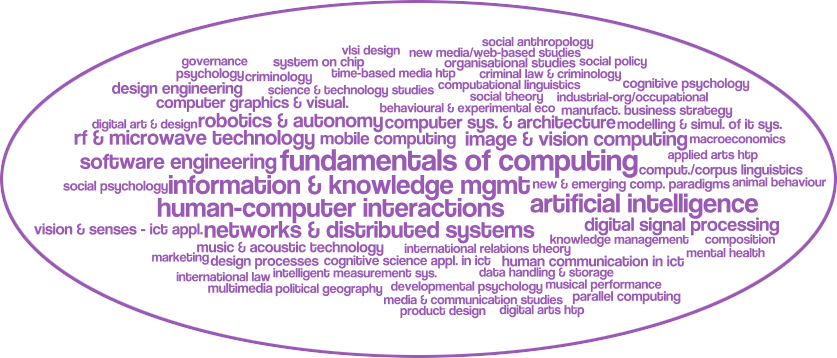
\includegraphics[width=14cm]{word-clouds/number/c2}
    \caption[Topics clustered within Community 2 in the \textit{Topic-grant} network]{Topics clustered within Community 2 in the \textit{Topic-grant} network. Font size represents the number of grants that each topic appears in.}
    \label{figure:topic_a_current_number_c2}
\end{figure}

\noindent\textbf{Community 3 (Energy, Power)} also represents a comprehensible clustering enclosing topics such as \textit{fluid dynamics}, \textit{aerodynamics}, \textit{bioenergy}, \textit{microsystems}, \textit{wind power} and \textit{energy - marine \& hydropower}. It consists of three major topics both in terms of number of grants that each topic appears in but also the value of those grants: \textit{materials characterisation} (270 grants, worth \pounds350M), \textit{materials synthesis \& growth} (273 grants, worth \pounds305M) and \textit{manufacturing machine \& plant} (196 grants worth \pounds273M). Figure \ref{figure:topic_a_current_number_c3} presents a word cloud representation of Community 3.

\clearpage

\begin{figure}[!htbp]
    \centering
    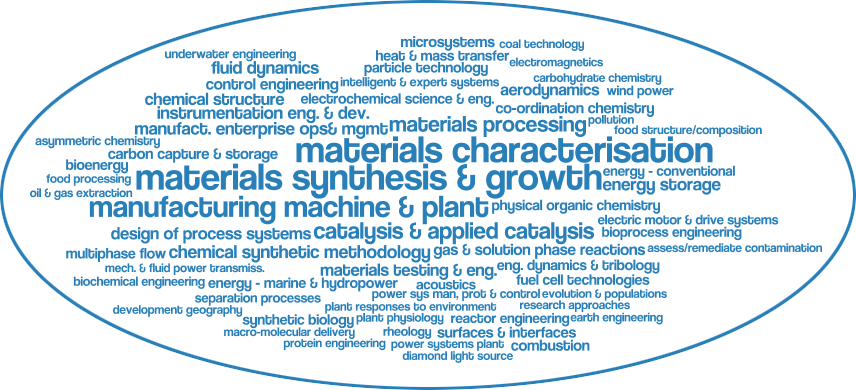
\includegraphics[width=13cm]{word-clouds/number/c3}
    \caption[Topics clustered within Community 3 in the \textit{Topic-grant} network]{Topics clustered within Community 3 in the \textit{Topic-grant} network. Font size represents the number of grants that each topic appears in.}
    \label{figure:topic_a_current_number_c3}
\end{figure}

\noindent\textbf{Community 4 (Mathematics)} is the smallest community in size (only 10 topics) but also the most well-defined community, as the topics clustered within it have a concrete, shared focus in Mathematics. It consists of research topics including \textit{algebra \& geometry}, \textit{mathematical physics} and \textit{continuum mechanics}. \textit{Algebra \& geometry} and \textit{statistics \& appl. probability} are the topics which appear in the highest number of grants, 131 and 120, respectively. In terms of value, the latter is valued higher than the former, \pounds200M compared to \pounds69M. Figure \ref{figure:topic_a_current_number_c4} presents a word cloud representation of Community 4.

\begin{figure}[!htbp]
    \centering
    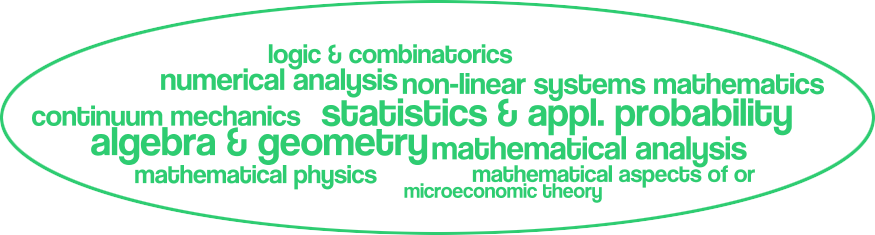
\includegraphics[width=13cm]{word-clouds/number/c4}
    \caption[Topics clustered within Community 4 in the \textit{Topic-grant} network]{Topics clustered within Community 4 in the \textit{Topic-grant} network. Font size represents the number of grants that each topic appears in.}
    \label{figure:topic_a_current_number_c4}
\end{figure}

\noindent\textbf{Community 5 (Environment)} represents a coherent clustering of topics including \textit{energy efficiency}, \textit{geohazards}, \textit{environment \& health} and \textit{urban \& land management}. This community represents topics from different fields which appear in grants that share an aim in tackling an environment-related problem such as climate change or global warming. The most popular topic in terms of number of grants is \textit{energy efficiency}, with 100 grants valued at \pounds150M. Figure \ref{figure:topic_a_current_number_c5} presents a word cloud representation of Community 5.

\begin{figure}[!htbp]
    \centering
    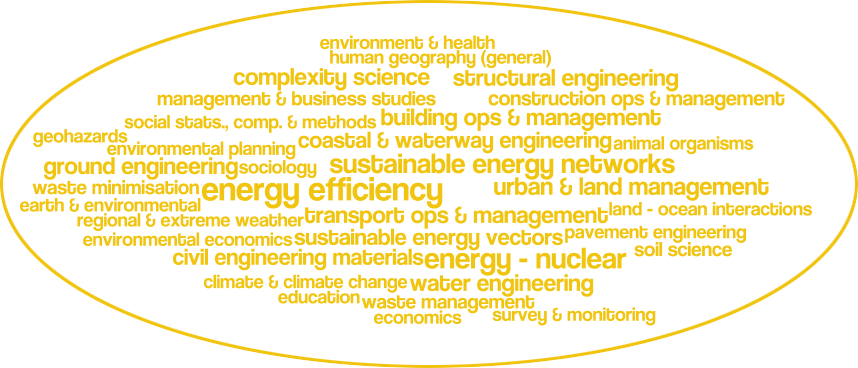
\includegraphics[width=13cm]{word-clouds/number/c5}
    \caption[Topics clustered within Community 5 in the \textit{Topic-grant} network]{Topics clustered within Community 5 in the \textit{Topic-grant} network. Font size represents the number of grants that each topic appears in.}
    \label{figure:topic_a_current_number_c5}
\end{figure}

\noindent\textbf{Community 6 (Physics, Electricity)} is the last identified community and another community which consists of a rational clustering of topics surrounding the fields of \textit{physics} and \textit{electricity}. Topics include \textit{solar technology}, \textit{biophysics} and \textit{electronic devices \& subsys.}. \textit{Condensed Matter Physics} is the topic that appears in in the highest number of grants, 82, worth \pounds97M. Figure \ref{figure:topic_a_current_number_c6} presents a word cloud representation of Community 6.

\begin{figure}[!htbp]
    \centering
    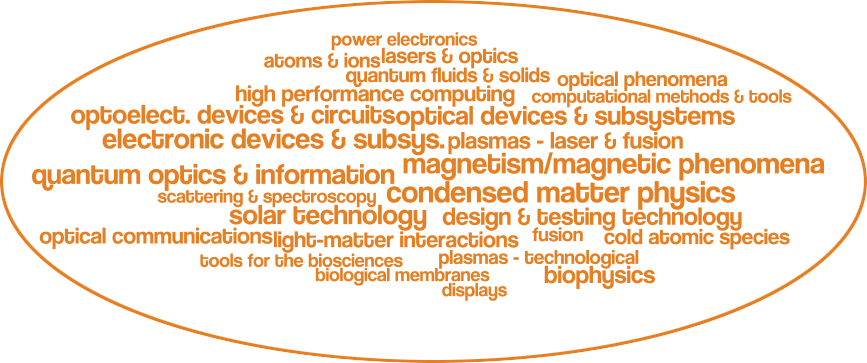
\includegraphics[width=14cm]{word-clouds/number/c6}
    \caption[Topics clustered within Community 6 in the \textit{Topic-grant} network]{Topics clustered within Community 6 in the \textit{Topic-grant} network. Font size represents the number of grants that each topic appears in.}
    \label{figure:topic_a_current_number_c6}
\end{figure}

\noindent Click \href{https://raw.githubusercontent.com/SergiuTripon/msc-thesis-na-epsrc/master/wiki/word-clouds/png/number/communities/modified/full.png?token=AJsbI8Ehc-UcfUTnOVKrCSgHqfUe3IoPks5X27kGwA\%3D\%3D}{\textcolor{blue}{\textbf{here}}} to view a full, high-resolution word cloud representation.

\clearpage

\subsubsection{Visualisation of community structure}

A visualisation of the community structure discovered in the current \textit{Topic-grant} network by the optimal solution identified, presented in Fig. \ref{figure:topic_a_current_cs}, was produced using iGraph. It features nodes in 6 different colours depending on which community they are clustered in. Edges between the nodes in each community are grey, while edges between nodes from different communities are excluded altogether. The size of the node circle represents the number of grants node attribute. The width of the edge line represents the number of grants edge attribute. The topics with the highest number of grants are identified by a darker shade of the colour assigned to their community.

\begin{figure}[htpb]
    \centering
    \fbox{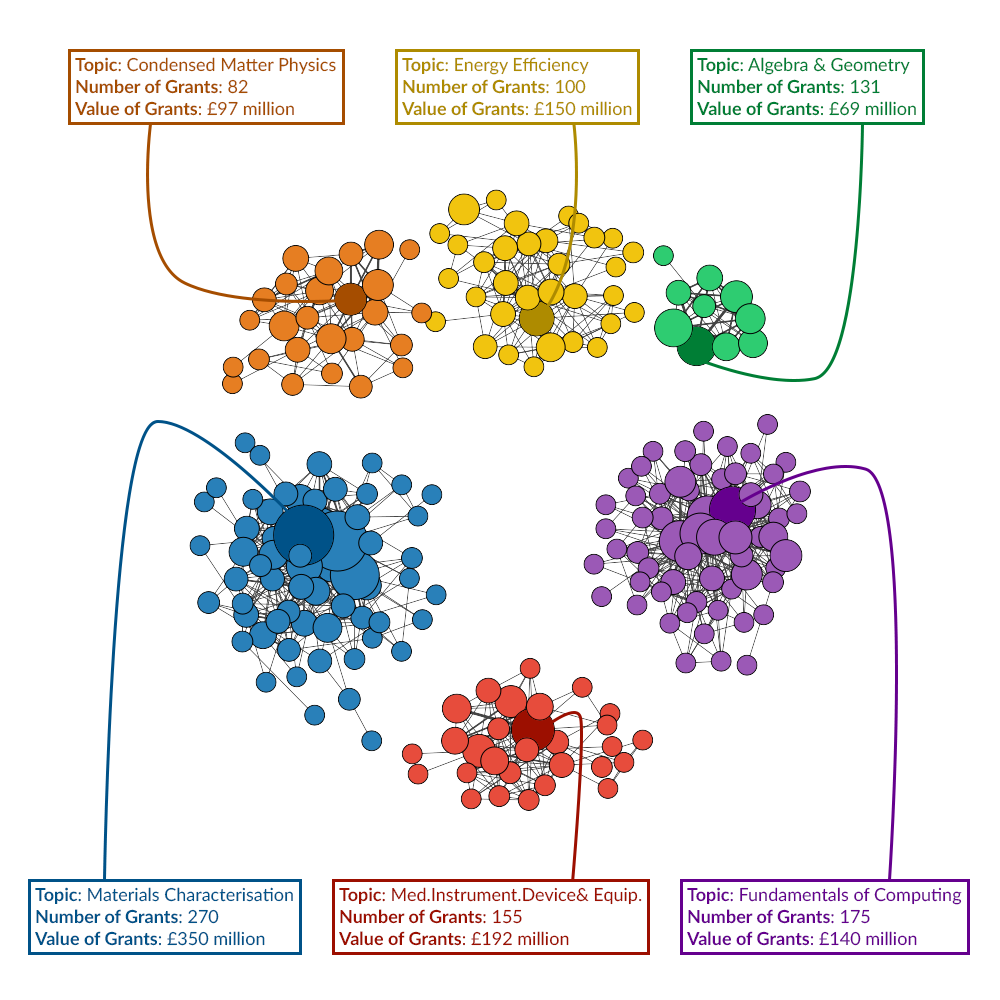
\includegraphics[width=13cm]{communities/topic_a_cs}}
    \caption[Visualisation of the community structure within the \textit{Topic-grant} network constructed using the current (2010 to 2016) data set.]{Visualisation of the community structure within the \textit{Topic-grant} network constructed using the current (2010 to 2016) data set. The topics with the highest number of grants are identified by a darker shade of the colour.}
    \label{figure:topic_a_current_cs}
\end{figure}

\subsection{Evaluation}

A strong network clustering means that a node pair within the same cluster will have a higher similarity compared to a node pair consisting of nodes from two different clusters. The purpose of the evaluation phase is to determine whether in reality this is also true.

First and foremost, the origin and destination nodes of each edge in the \textit{Topic-grant} network were identified. This forms a pair of nodes as follows: (origin node, destination node). Certain edges link nodes that are in the same cluster, while others link nodes that are in different clusters. Therefore, some node pairs represent nodes from the same cluster, while others represent nodes from different clusters. Subsequently, the Dice and Jaccard similarity between each node pair was calculated. Finally, in order to obtain an overall perspective of the similarity of nodes within and between clusters, the average Dice and Jaccard similarity was calculated. 

Indeed, the results show that for both the current and historical Topic-grant networks, nodes within the same cluster have a higher similarity than nodes from different clusters. Table \ref{table:topic_a_evaluation} presents the results of the evaluation phase carried out on the Topic-grant network constructed using both the historical (1990 to 2010) and current (2010 to 2016) data sets.

\begin{table}[htbp]
\centering
\caption[Dice and Jaccard similarity coefficients of node pairs within and between clusters in the Topic-grant constructed using both the historical (1990 to 2010) and current (2010 to 2016) data sets.]{Dice and Jaccard similarity coefficients of node pairs within and between clusters in the Topic-grant network constructed using both the historical (1990 to 2010) and current (2010 to 2016) data sets. Each node pair represents an edge which links two nodes from the same cluster or two different clusters. \textbf{IN} stands for within communities, while \textbf{OUT} means between communities.}
\label{table:topic_a_evaluation}
\begin{tabular}{r|rrr}
{} & \textbf{1990-2000} & \textbf{2000-2010} & \textbf{2010-2016}\\
\hline\\
Node pairs IN                  & {437}   & {1940}  & {1122}\\
Node pairs OUT                 & {311}   & {1652}  & {886}\\
Average Dice similarity IN     & {0.465} & {0.510} & {0.428}\\
Average Dice similarity OUT    & {0.346} & {0.433} & {0.354}\\
Difference between IN and OUT  & {0.119} & {0.077} & {0.074}\\
Average Jaccard similarity IN  & {0.316} & {0.356} & {0.286}\\
Average Jaccard similarity OUT & {0.217} & {0.283} & {0.220}\\
Difference between IN and OUT  & {0.099} & {0.073} & {0.066}\\
\end{tabular}
\end{table}

\clearpage

\subsection{Discussion}

The \textit{Topic-grant} network was constructed using both the historical (1990 to 2010) and current (2010 to 2016) data sets. This means a comparative analysis can be conducted comparing the data sets in terms of research trend and funding, and clustering.

\subsubsection{Comparison to historical data}

Over the years, the research trend led to new topics being defined, while others were discontinued. For example, \textit{bionanoscience}, \textit{escience} and \textit{language acquisition} are topics which existed \textit{from 2000 to 2010} but do not exist currently. In contrast, \textit{animal organisms}, \textit{political geography} and \textit{ageing: chemistry/biochemistry} are some of the current topics that were defined after 2010.

Similarly, the funding trend also evolved as more recent grants saw a significant increase in the funding support provided. Currently, there are 3,072 grants within communities with a total value of \pounds3.5B. Between 2000 and 2010, researchers worked on 16,617 grants, valued at \pounds4.9B. These figures indicate a significant difference in the number of grants. However, this is justified, as the two time periods compared are not equal, as the former covers 6 years of grants, while the latter covers 10 years. More importantly, the difference in value is not considerable, which shows the progress of research funding over the years, as current grants receive significantly more funding than they would have 10 years ago.

Furthermore, this is also supported by the number and value of grants completed between 1990 and 2000. Researchers worked on a slightly less number of grants than between 2000 and 2010, but they also received significantly less funding, \pounds1.7B. Tables \ref{table:topic_a_past1_numbers} and \ref{table:topic_a_past2_numbers} present the number of nodes representing topics, the number and value of grants and the predominant words within each community in the \textit{Topic-grant} network constructed using the historical (2000 to 2010) data set and historical (1990 to 2000) data set, respectively.

\clearpage

\begin{table}[!htbp]
\centering
\caption[Number of nodes and grants, value of grants and the predominant words of each community identified in the \textit{Topic-grant} network constructed using the historical (2000 to 2010) data set]{Number of nodes and grants, value of grants and the predominant words based on word frequency of each community identified in the \textit{Topic-grant} network constructed using the historical (2000 to 2010) data set. The number of grants includes duplicate grants, as a grant can be part of more than one community. Subsequently, the value of grants also includes the duplicate grants. However, the last column represents the number and value of unique grants in communities within the historical \textit{Topic-grant} network.}
\label{table:topic_a_past1_numbers}
\begin{tabular}{r|>{\raggedleft\arraybackslash}p{1.6cm}>{\raggedleft\arraybackslash}p{1.6cm}>{\raggedleft\arraybackslash}p{1.6cm}>{\raggedleft\arraybackslash}p{6.3cm}}
{} & \textbf{Number (topics)} & \textbf{Number (grants)} & \textbf{Value (grants)} & \textbf{Predominant words based on word frequency}\\
\hline\\
\textbf{C1}  & {67}  & {8682}  & {\pounds2.6B} & {chemistry, biology, science}\\
\textbf{C2}  & {43}  & {5167}  & {\pounds1.3B} & {engineering, mathematical}\\
\textbf{C3}  & {25}  & {1394}  & {\pounds699M} & {energy, power}\\
\textbf{C4}  & {2}   & {1}     & {\pounds1M}   & {science}\\
\textbf{C5}  & {71}  & {4099}  & {\pounds1.3B} & {design, arts, digital}\\
\hline\\
\textbf{All} & {208} & {16617} & {\pounds4.9B} & {engineering, biology, design}\\
\end{tabular}
\end{table}

In terms of clustering, the historical communities identified within the \textit{Topic-grant} network hold slight differences when compared to the current communities. First and foremost, the community detection algorithm identified 5 communities in both historical (1990 to 2000, 2000 to 2016) networks. This decrease may signify the result of the contrast in the number of topics and the actual topics between the current and historical networks. Moreover, the most well-defined, Community 4 (Mathematics) identified in the current \textit{Topic-grant} network, is not as well-defined anymore in the historical network, as it is part of a larger community in Community 2 (Engineering, Mathematics ). This symbolises the current increase in the number of grants that are focused on \textit{mathematics} only, rather than a combined effort including other topics such as \textit{engineering}. Furthermore, between 2000 and 2010, only one grant was classified simultaneously by \textit{soil science} and \textit{crop science}. In the current (2010 to 2016) data set, \textit{crop science} is not present anymore. Perhaps, its removal could be justified by the similarity between the two topics, deeming one of them as unnecessary. This also indicates a potential reason why the two topics did not form a community in the current \textit{Topic-grant} network.

\begin{table}[!htbp]
\centering
\caption[Number of nodes and grants, value of grants and the predominant words of each community identified in the \textit{Topic-grant} network constructed using the historical (1990 to 2000) data set]{Number of nodes and grants, value of grants and the predominant words based on word frequency of each community identified in the \textit{Topic-grant} network constructed using the historical (1990 to 2000) data set. The number of grants includes duplicate grants, as a grant can be part of more than one community. Subsequently, the value of grants also includes the duplicate grants. However, the last column represents the number and value of unique grants in communities within the historical \textit{Topic-grant network}.}
\label{table:topic_a_past2_numbers}
\begin{tabular}{r|>{\raggedleft\arraybackslash}p{1.6cm}>{\raggedleft\arraybackslash}p{1.6cm}>{\raggedleft\arraybackslash}p{1.6cm}>{\raggedleft\arraybackslash}p{6.3cm}}
{} & \textbf{Number (topics)} & \textbf{Number (grants)} & \textbf{Value (grants)} & \textbf{Predominant words based on word frequency}\\
\hline\\
\textbf{C1}  & {28}  & {2015}  & {\pounds246M} & {engineering, energy, management}\\
\textbf{C2}  & {25}  & {3995}  & {\pounds661M} & {optical, devices, materials}\\
\textbf{C3}  & {17}  & {1328}  & {\pounds88M}  & {mathematical, analysis}\\
\textbf{C4}  & {39}  & {3455}  & {\pounds496M} & {engineering, ict, design}\\
\textbf{C5}  & {27}  & {2567}  & {\pounds385M} & {chemistry, catalysis, energy}\\
\hline\\
\textbf{All} & {136} & {12791} & {\pounds1.7B} & {engineering, chemistry, systems}\\
\end{tabular}
\end{table}

\subsubsection{Motivation for the Topic-researcher network}

The \textit{Topic-researcher} network represents an alternative and another way of interpreting the topic data to construct a network. An alternative represents a different perspective on the data. The \textit{Topic-grant} network is one way of analysing topics, from the point of view of grants. The \textit{Topic-researcher} network is a second way of analysing topics, from the point of view of researchers. Grant records and researcher records are significantly different, and one may provide different or better results than the other. Furthermore, having a different way of analysing the data means that a comparative analysis of the results can be carried out. Therefore, both networks are considered important due to the different and valuable insights that can be translated from the data.

\clearpage

\section{Clustering of Topic-researcher network}

The process of clustering the \textit{Topic-researcher} network involves a number of different stages including carrying out experiments, producing results, evaluating results as well as conducting comparative analysis.

\subsection{Experiment}

In order to ensure a consistent comparative analysis between the two Topic networks, the optimal solution identified as a result of the experiment on the \textit{Topic-grant} network, is also considered the optimal solution for the \textit{Topic-researcher} network. However, the experiment was still carried out and the results are presented in Tables 1.31-1.33, part of the Supplementary material.

\subsection{Results}

The application of the optimal solution identified on the \textit{Topic-researcher} network resulted in the identification of 4 different communities of topics, 2 less than within the \textit{Topic-grant} network. Note that the \textit{Topic-researcher} network was constructed using the current (2010 to 2016) data set only, as researcher records within EPSRC only provide the current topics of a researcher. Table \ref{table:topic_b_current_numbers} presents the number of nodes representing topics and the predominant words within each community discovered in the \textit{Topic-researcher} network. The complete clustering of the \textit{Topic-researcher} network is presented in Table \ref{table:topic_b_current_clusters_appendix}, part of Appendix \ref{appendix:epsrc_grant_data}.

\begin{table}[!htbp]
\centering
\caption[Number of nodes and the predominant words of each community identified in the \textit{Topic-researcher} network constructed using the current (2010 to 2016) data set]{Number of nodes and the predominant words based on word frequency of each community identified within the \textit{Topic-researcher} network constructed using the current (2010 to 2016) data set.}
\label{table:topic_b_current_numbers}
\begin{tabular}{r|>{\raggedleft\arraybackslash}p{1.6cm}>{\raggedleft\arraybackslash}p{6.5cm}}
{} & \textbf{Number (topics)} & \textbf{Predominant words based on frequency of words}\\
\hline\\
\textbf{C1}  & {39}  & {engineering, management}\\
\textbf{C2}  & {62}  & {psychology, design}\\
\textbf{C3}  & {15}  & {mathematical, analysis}\\
\textbf{C4}  & {109} & {engineering, chemistry}\\
\hline\\
\textbf{All} & {225} & {engineering, management, science}\\
\end{tabular}
\end{table}

\subsubsection{Visualisation of community structure}

Similarly to the \textit{Topic-grant} network, a visualisation of the community structure discovered in the current \textit{Topic-researcher} network was produced and is presented in Fig. \ref{figure:topic_b_current_cs}.

\begin{figure}[htpb]
    \centering
    \fbox{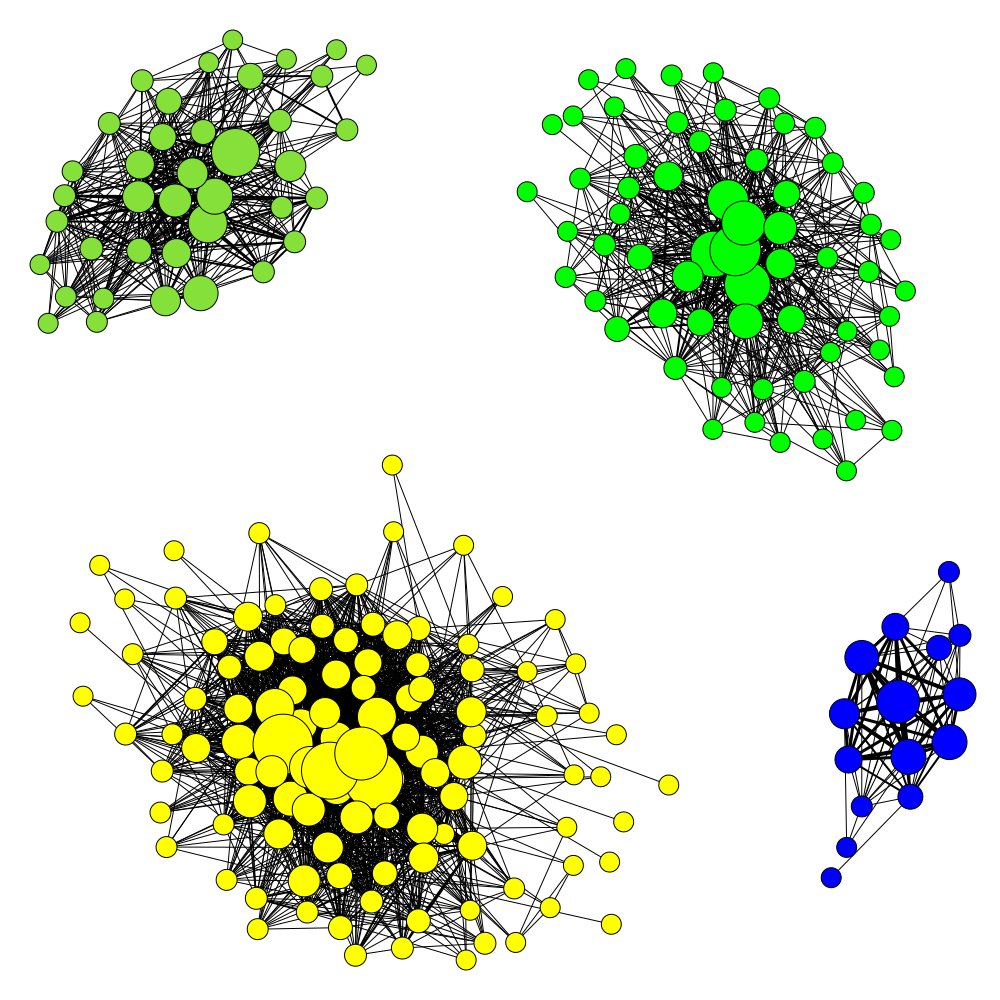
\includegraphics[width=13.8cm]{communities/topic_b_cs}}
    \caption[Visualisation of the community structure within the Topic-researcher network constructed using the current (2010 to 2016) data set.]{Visualisation of the community structure within the Topic-researcher network constructed using the current (2010 to 2016) data set.}
    \label{figure:topic_b_current_cs}
\end{figure}

\subsection{Evaluation}

Similarly to the \textit{Topic-grant} network, the \textit{Topic-researcher} network also underwent the evaluation phase and the results show that for both the current and historical \textit{Topic-researcher} networks, nodes within the same cluster have a higher similarity than nodes from different clusters. Table \ref{table:topic_b_evaluation} presents the results of the evaluation phase carried out on the \textit{Topic-researcher} network constructed using the current (2010 to 2016) data set.

\begin{table}[htpb]
\centering
\caption[Dice and Jaccard similarity coefficients of node pairs within and between clusters in the \textit{Topic-researcher} constructed using the current (2010 to 2016) data set.]{Dice and Jaccard similarity coefficients of node pairs within and between clusters in the \textit{Topic-researcher} network constructed using the current (2010 to 2016) data set. Each node pair represents an edge which links two nodes from the same cluster or two different clusters. \textbf{IN} stands for within communities, while \textbf{OUT} means between communities.}
\label{table:topic_b_evaluation}
\begin{tabular}{r|r}
{} & \textbf{2010-2016}\\
\hline\\
Node pairs IN                  & {2921}\\
Node pairs OUT                 & {2271}\\
Average Dice similarity IN     & {0.543}\\
Average Dice similarity OUT    & {0.517}\\
Difference between IN and OUT  & {0.026}\\
Average Jaccard similarity IN  & {0.393}\\
Average Jaccard similarity OUT & {0.359}\\
Difference between IN and OUT  & {0.034}\\
\end{tabular}
\end{table}

\subsection{Discussion}

The \textit{Topic-grant} and \textit{Topic-researcher} networks represent two interpretations of the topic data. This means a comparative analysis can be conducted comparing the two networks in terms of clustering.

\subsubsection{Comparison to Topic-grant network}

There are obvious differences between the clustering produced using the \textit{Topic-grant} network and \textit{Topic-researcher} network. Firstly, the number of communities identified differs, as using the former 6 communities were identified, compared to 4 when using the latter. This results in an imbalance in community size, with one of the communities (Community 4) identified in the \textit{Topic-researcher} network consisting of 109 topics. A large community is also a broad community, which means that is less specific and lacks the capability to represent one or more clear research areas. It also causes other communities to be significantly smaller in size.

\clearpage

Furthermore, the \textit{Mathematics} community (Community 4) identified using the \textit{Topic-grant} network is larger in size and its previously well-defined structure is "harmed" by the irrational addition of topics such as \textit{genomics} when identified  using the \textit{Topic-researcher} network. Moreover, the clustering produced using the \textit{Topic-researcher} network also failed to identify the \textit{Biology} community (Community 1) which was successfully identified using the \textit{Topic-grant} network. That being said, there are also similarities between the communities identified using the two networks, as the \textit{Engineering} and \textit{Chemistry} communities appear in the community structure of both networks.

In conclusion, it is concluded that the clustering produced using the \textit{Topic-grant} network is more coherent and balanced than the one produced using the \textit{Topic-researcher} network.
\chapter{\textsc{Networks of Researchers}}
\label{chapter:networks_of_researchers}

The idea behind a network of researchers involves two ways that the network can be constructed. Likewise, the researchers within the network can be analysed from the perspective of grants as well as topics. Technically speaking, nodes in the network will represent researchers regardless of perspective. However, edges can represent either grants or topics. In the end, two different networks of researchers are constructed, the \textit{Researcher-grant} network and the \textit{Researcher-topic} network.

\section{Researcher-grant network}

The \textit{Researcher-grant} network consists of nodes representing researchers and edges representing grants. The \textit{Principal} and \textit{Other Investigators} fields in each grant record consist of one or more researchers that collaborate on the grant. Only grant records with two or more researchers were included in the analysis. Subsequently, a link between each researcher and all other researchers within each grant record was established. The link signifies the grant record that the researchers all have in common, and is represented as an edge in a network. Due to the significantly large size of the \textit{Researcher-grant} network, the network had to be sampled with the sample consisting of nodes connected by edges with an edge weight of 2 or more. Fig. \ref{figure:researcher_b_structure} provides a visual explanation of how the \textit{Researcher-grant} network was constructed using the collected EPSRC data, including the formulated node and edge attributes.

\begin{figure}[htpb]
    \centering
    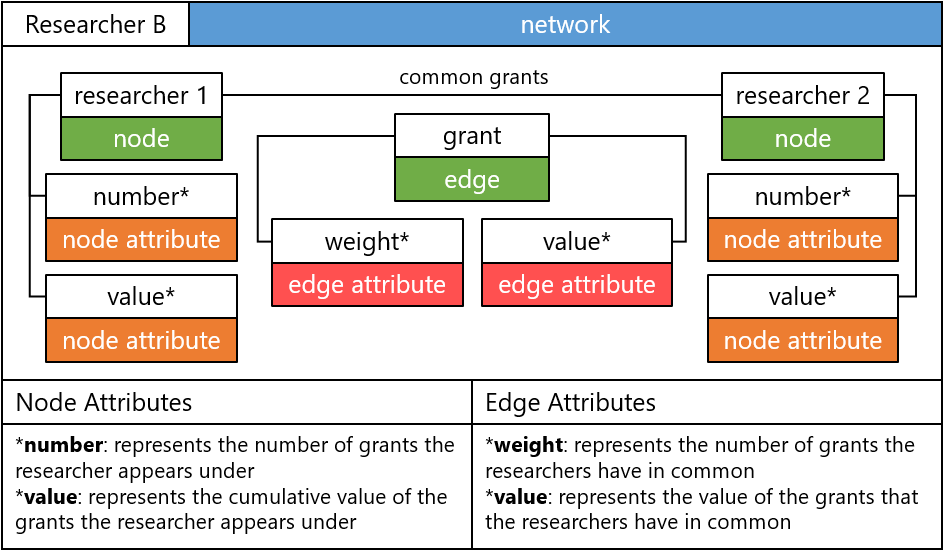
\includegraphics[width=8cm]{networks-explained/researcher_network_b}
    \caption[Visual explanation of how the \textit{Researcher-grant} network was structured and constructed using the collected EPSRC data]{Visual explanation of how the \textit{Researcher-grant} network was structured and constructed using the collected EPSRC data, including the formulated node and edge attributes.}
    \label{figure:researcher_b_structure}
\end{figure}

\subsection{Node and edge attributes}

The \textit{Researcher-grant} network contains two different node and edge attributes, the number and value of grants. Node and edge attributes are common between networks. Consequently, their formulation is considered a common task, and therefore it is described in Chapter \ref{chapter:methodology}: Methodology.

\subsection{Properties of Researcher-grant network}

The \textit{Researcher-grant} network is a carbon copy of the \textit{Topic-grant} network, with the exception that, in this case, nodes represent researchers and not topics. Table \ref{table:researcher_b_properties} presents the properties of both the historical and current \textit{Researcher-grant} networks.

\begin{table}[htbp]
\centering
\caption[Properties of the \textit{Researcher-grant} network constructed using both the historical (1990 to 2010) and current (2010 to 2016) data sets]{Properties of the \textit{Researcher-grant} network constructed using both the historical (1990 to 2010) and current (2010 to 2016) data sets.}
\label{table:researcher_b_properties}
\begin{tabular}{r|rrr}
{} & \textbf{1990-2000} & \textbf{2000-2010} & \textbf{2010-2016}\\
\hline\\
\textbf{Nodes}                          & {1847}   & {2434}    & {260}\\
\textbf{Edges}                          & {2002}   & {4919}    & {208}\\
\textbf{Type}                           & {Undirected} & {Undirected} & {Undirected}\\
\textbf{Weighted}                       & {Yes}    & {Yes}     & {Yes}\\
%\textbf{Connected}                     & {No}     & {No}      & {No}\\
\textbf{Average Degree}                 & {2.168}  & {4.042}   & {1.60}\\
\textbf{Average Weighted Degree}        & {2.798}  & {7.794}   & {2.592}\\
\textbf{Diameter}                       & {18.0}   & {36.0}    & {16.0}\\
%\textbf{Radius}                        & {1.0}    & {1.0}     & {1.0}\\
\textbf{Density}                        & {0.001}  & {0.002}   & {0.006}\\
\textbf{Modularity}                     & {0.978}  & {0.977}   & {0.955}\\
%\textbf{Communities}                   & {563}    & {485}     & {91}\\
%\textbf{Weak Components}                & {559}    & {473}     & {89}\\
%\textbf{Node Closeness}                & {0.001}  & {0.0}     & {0.004}\\
%\textbf{Node Betweenness}              & {14.214} & {138.711} & {1.965}\\
%\textbf{Edge Betweenness}              & {17.545} & {79.157}  & {4.625}\\
\textbf{Average Clustering Coefficient} & {0.648}  & {0.748}   & {0.578}\\
%\textbf{Eigenvector Centrality}        & {0.005}  & {0.007}   & {0.016}\\
\textbf{Average Path Length}            & {3.676}  & {6.874}   & {1.942}\\
\end{tabular}
\end{table}

The current \textit{Researcher-grant} network is composed of 260 nodes and 208 edges representing one or more common grants between two researchers. The network features a significantly disconnected structure, shown in Fig. \ref{figure:researcher_b_current_vis}, which is primarily due to the rarity in repeated collaboration among researchers on EPSRC-supported grants, which may last up to 8 years.

Furthermore, both historical \textit{Researcher-grant} networks consist of both an increased number of nodes and edges when compared to their current data equivalent. Furthermore, all three networks are weighted and in the in the creation of Table \ref{table:researcher_b_properties} and Fig. \ref{figure:researcher_b_current_vis}, the number of grants edge weight attribute is used.

\subsection{Visualisation of Researcher-grant network}

A visualisation of the \textit{Researcher-grant} network, presented in Fig. \ref{figure:researcher_b_current_vis}, was produced. It features nodes in blue, and edges in grey. The size of the node circle represents the number of grants node attribute. The width of the edge line represents the number of grants edge attribute. The researcher(s) that appear in the highest number of grant records are coloured in red.

\begin{figure}[htpb]
    \centering
    \fbox{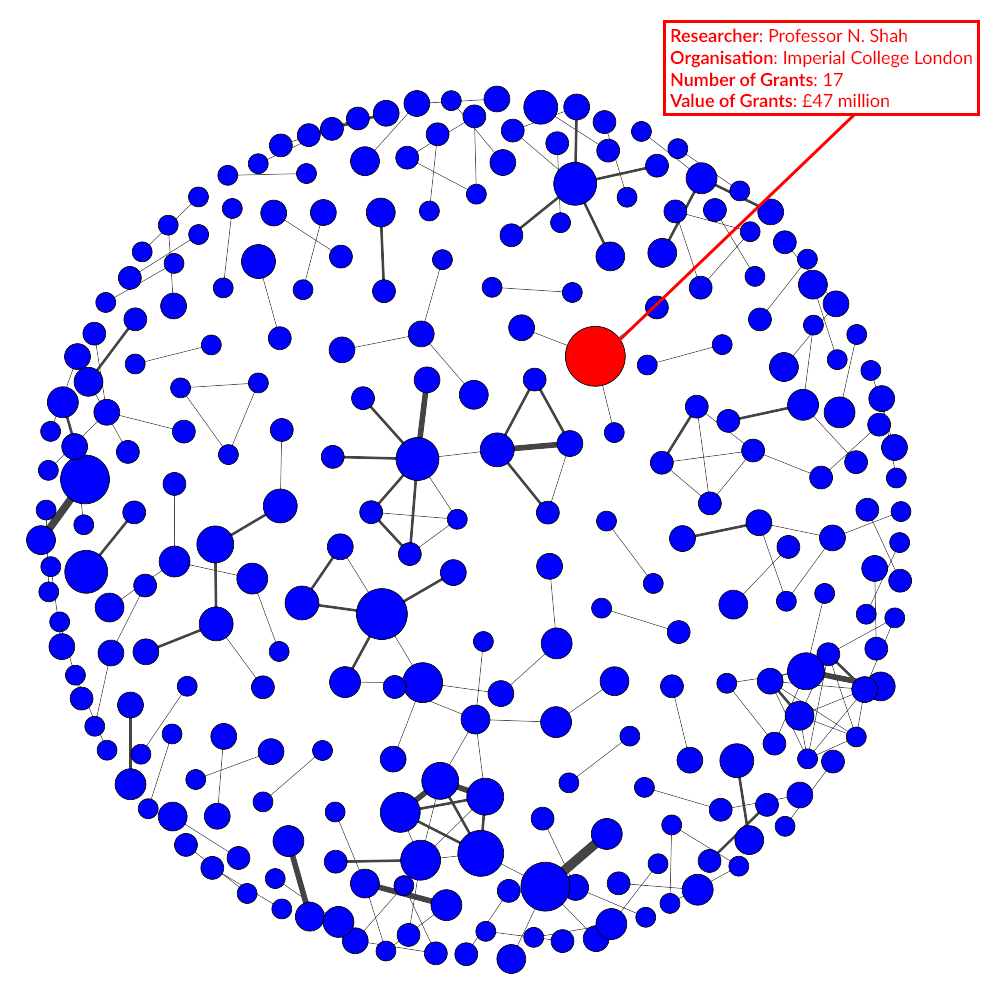
\includegraphics[width=12cm]{networks/researcher_b}}
    \caption[Visualisation of the \textit{Researcher-grant} network constructed using the current (2010 to 2016) data set.]{Visualisation of the \textit{Researcher-grant} network constructed using the current (2010 to 2016) data set. The researcher(s) that appear in the highest number of grant records are coloured in red.}
    \label{figure:researcher_b_current_vis}
\end{figure}

\section{Researcher-topic network}

The \textit{Researcher-topic} network consists of nodes representing researchers and edges representing topics. The \textit{Current EPSRC-Supported Research Topics} field in each researcher record consists of one or more topics that classify the grants supported by EPSRC that the researcher is currently an investigator in. Only researcher records with two or more topics were included in the analysis. Subsequently, each researcher record was compared to all other researcher records, and if they had at least one topic in common a link between the two researchers was established. The link signifies the topic(s) that two researchers have in common, and is represented as an edge in a network. Due to its significantly large size, the \textit{Researcher-topic} network was sampled and only includes nodes connected by edges with an edge weight of 5 or more. Fig. \ref{figure:researcher_a_structure} provides a visual explanation of how the \textit{Researcher-topic} network was constructed using the collected EPSRC data, including the formulated node and edge attributes.

\begin{figure}[htpb]
    \centering
    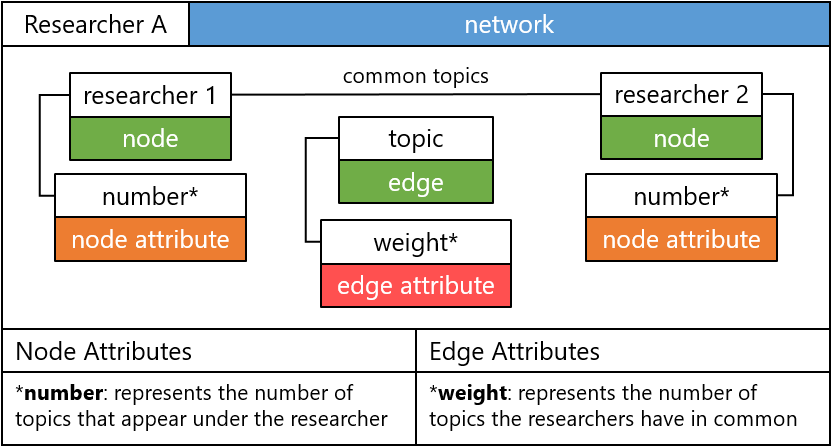
\includegraphics[width=8cm]{networks-explained/researcher_network_a}
    \caption[Visual explanation of how the \textit{Researcher-topic} network was structured and constructed using the collected EPSRC data]{Visual explanation of how the \textit{Researcher-topic} network was structured and constructed using the collected EPSRC data, including the formulated node and edge attributes.}
    \label{figure:researcher_a_structure}
\end{figure}

\subsection{Node and edge attributes}

The \textit{Researcher-topic} network contains one node and edge attribute, the number of topics. In the \textit{Researcher-topic network} edges represent topics, therefore, it does not contain the value of grants attribute. Node and edge attributes are common between networks. Consequently, their formulation is considered a common task, and therefore it is described in Chapter \ref{chapter:methodology}: Methodology.

\subsection{Properties of Researcher-topic network}

The \textit{Researcher-topic} network is a reversed version of the \textit{Topic-researcher} network. It consists of 655 researchers linked by 4548 edges representing common topics between the researchers. Table \ref{table:researcher_a_properties} presents the properties of the \textit{Researcher-topic} network.

\begin{table}[htbp]
\centering
\caption[Properties of the \textit{Researcher-topic} network constructed using the current (2010 to 2016) data set]{Properties of the \textit{Researcher-topic} network constructed using the current (2010 to 2016) data set.}
\label{table:researcher_a_properties}
\begin{tabular}{r|r}
{} & \textbf{2010-2016}\\
\hline\\
\textbf{Nodes}                          & {655}\\
\textbf{Edges}                          & {4548}\\
\textbf{Type}                           & {Undirected}\\
\textbf{Weighted}                       & {Yes}\\
%\textbf{Connected}                     & {No}\\
\textbf{Average Degree}                 & {13.887}\\
\textbf{Average Weighted Degree}        & {27.258}\\
\textbf{Diameter}                       & {15.0}\\
%\textbf{Radius}                        & {1.0}\\
\textbf{Density}                        & {0.021}\\
\textbf{Modularity}                     & {0.738}\\
%\textbf{Communities}                   & {49}\\
%\textbf{Weak Components}                & {39}\\
%\textbf{Node Closeness}                & {0.005}\\
%\textbf{Node Betweenness}              & {703.138}\\
%\textbf{Edge Betweenness}              & {127.386}\\
\textbf{Average Clustering Coefficient} & {0.825}\\
%\textbf{Eigenvector Centrality}        & {0.078}\\
\textbf{Average Path Length}            & {4.278}\\
\end{tabular}
\end{table}

In comparison to the current \textit{Researcher-grant} network which consists of 260 nodes and 208 edges, this network consists of substantially more nodes and edges. Due to its significantly large size, the \textit{Researcher-topic} network had to be sampled with the sample consisting of nodes connected by edges with an edge weight of 5 or more. Furthermore, the network is undirected and weighted and in the creation of Table \ref{table:researcher_a_properties} and Fig. \ref{figure:researcher_a_vis}, the number of topics edge weight attribute is used.

\subsection{Visualisation of the Research-topic network}

A visualisation of the \textit{Researcher-topic} network, presented in Fig. \ref{figure:researcher_a_vis}, was produced using iGraph. It features nodes in blue, and edges in grey. The size of the node circle represents the number of topics node attribute. The width of the edge line represents the number of topics edge attribute. The researcher(s) with the highest number of topics are coloured in red.

As illustrated in Fig. \ref{figure:researcher_a_vis}, the structure of the \textit{Researcher-topic} network stands out from the others. Both \textit{Topic} networks feature a conglomeration of nodes densely connected. In contrast, the \textit{Researcher-grant} network consists the opposite of that, as it is sparsely connected with up to a maximum of 4 connected nodes. The \textit{Researcher-topic} network represents a combination between the two. Based on an initial observation, an unsurprising guess would indicate that a community detection algorithm has already been applied to this network. However, it has not, as its structure clearly resembles the layout of collaboration between researchers. Several small groups of researchers, densely connected internally, but sparsely connected externally, can be spotted. This can also translate to the assumption that the communities represent common topic interests between researchers.

\begin{figure}[htpb]
    \centering
    \fbox{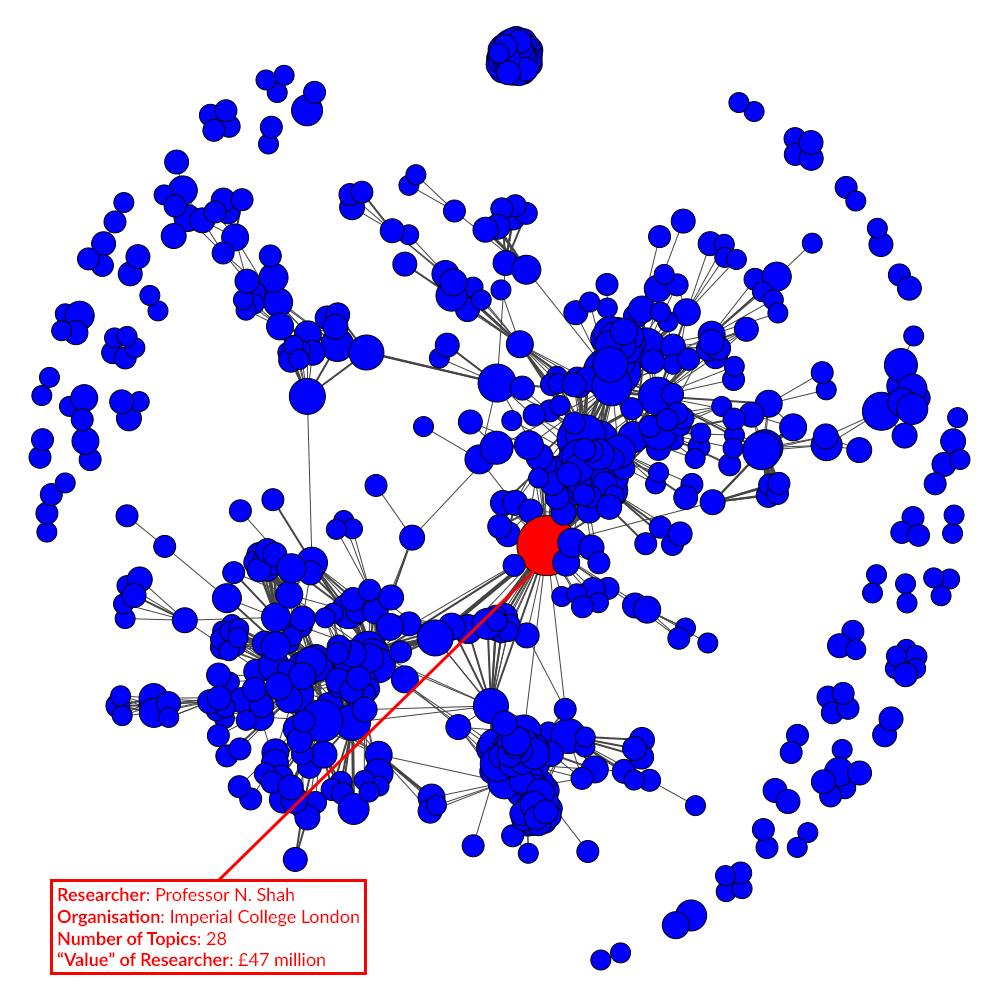
\includegraphics[width=11.5cm]{networks/researcher_a}}
    \caption[Visualisation of the \textit{Researcher-topic} network constructed using the current (2010 to 2016) data set]{Visualisation of the \textit{Researcher-topic} network constructed using the current (2010 to 2016) data set. The researcher(s) with the highest number of topics are coloured in red.}
    \label{figure:researcher_a_vis}
\end{figure}
\chapter{\textsc{Clustering of Researchers}}
\label{chapter:clustering_of_researchers}

This chapter describes the process of clustering the \textit{Researcher-grant} and \textit{Researcher-topic} networks. The experiments are detailed, while the results are presented. Additionally, results are evaluated and discussed through comparisons to historical data and between the two \textit{Researcher} networks.

\section{Clustering of Researcher-grant network}

The process of clustering the \textit{Topic-grant} network involves a number of different stages including carrying out experiments, producing results, evaluating results as well as conducting comparative analysis.

\subsection{Experiment}

Due to the limited amount of time available and in order to ensure a consistent comparative analysis, the optimal solution identified as a result of the experiment on the \textit{Topic-grant} network, is also considered the optimal solution for the \textit{Researcher-grant} network. However, the experiment was still carried out and the results are presented in Tables 1.36-1.38, 1.43-1.45 and 1.49-1.51, part of the Supplementary material.

\subsection{Results}

The application of the optimal solution identified on the \textit{Researcher-grant} network resulted in the initial and excessive identification of 89 communities of researchers, which signifies the lack of strong and frequent collaboration relationships between researchers. Table \ref{table:researcher_b_current_numbers} presents the number of nodes representing researchers and the number and value of grants within each community discovered in the current \textit{Researcher-grant} network.

\begin{table}[!htbp]
\centering
\caption[Number of nodes and grants and value of grants within the 2 largest communities in the \textit{Researcher-grant} network constructed using the current data set (2010 to 2016)]{Number of nodes and grants and value of grants within the 2 largest communities identified in the \textit{Researcher-grant} network constructed using the current data set (2010 to 2016). The number of grants includes duplicate grants, as a grant can be part of more than one community. Subsequently, the value of grants also includes the duplicate grants. However, the last column represents the number and value of unique grants in communities within the current \textit{Researcher-grant} network.}
\label{table:researcher_b_current_numbers}
\begin{tabular}{r|rrrr}
{} & \textbf{C1} & \textbf{C2} & \textbf{Total}\\
\hline\\
\textbf{Number of researchers} & {10} & {12} & {22}\\
\textbf{Number of grants}      & {33} & {35} & {65}\\
\textbf{Value of grants} & {\pounds103M} & {\pounds87M} & {\pounds177M}\\
\end{tabular}
\end{table}

Consequently, it seems that two or more researchers collaborating multiple times as part of a grant is a rarity within the collected EPSRC data. Due to the sparse nature of the communities identified, only the two largest communities are presented in the report.

\subsubsection{Visualisation of community structure}

Similarly to the \textit{Topic-grant} network, a visualisation of the community structure discovered in the current \textit{Researcher-grant} network was produced and is presented in Fig. \ref{figure:researcher_b_current_cs}.

\begin{figure}[htpb]
    \centering
    \fbox{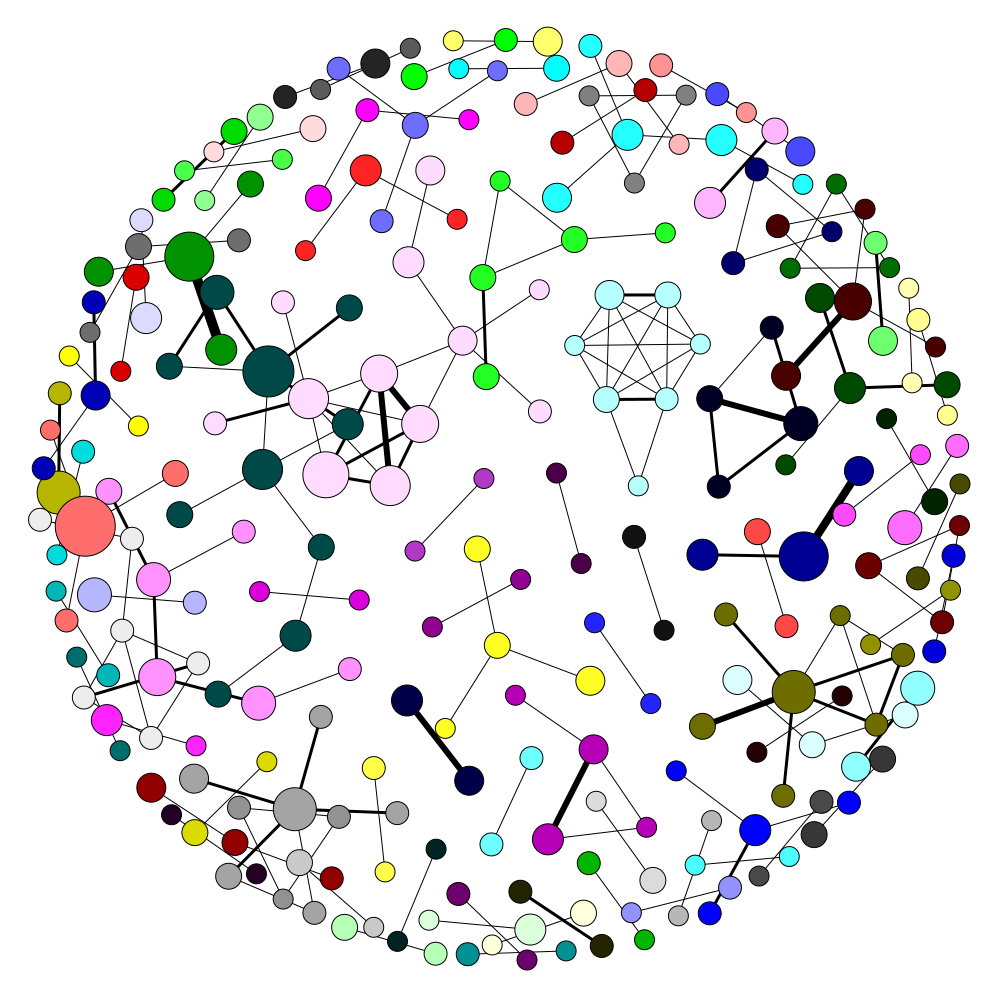
\includegraphics[width=12cm]{communities/researcher_b_cs}}
    \caption[Visualisation of the community structure within the \textit{Researcher-grant} network constructed using the current (2010 to 2016) data set]{Visualisation of the community structure within the \textit{Researcher-grant} network constructed using the current (2010 to 2016) data set.}
    \label{figure:researcher_b_current_cs}
\end{figure}

\subsection{Evaluation}

Similarly to the \textit{Topic-grant} network, the \textit{Researcher-grant} network also underwent the evaluation phase and the results show that for both the current and historical \textit{Researcher-grant} networks, nodes within the same cluster have a higher similarity than nodes from different clusters. Table \ref{table:researcher_b_evaluation} presents the results of the evaluation phase carried out on the \textit{Researcher-grant} network constructed using both the historical (1990 to 2000, 2000 to 2010) and  current (2010 to 2016) data sets.

\begin{table}[htpb]
\centering
\caption[Dice and Jaccard similarity coefficients of node pairs within and between communities in the \textit{Researcher-grant} network constructed using both the historical (1990 to 2010) and current (2010 to 2016) data sets]{Dice and Jaccard similarity coefficients of node pairs within and between communities in the \textit{Researcher-grant} network constructed using both the historical (1990 to 2010) and current (2010 to 2016) data sets. Each node pair represents an edge which connects two nodes within the same community or in two different communities. \textbf{IN} stands for within communities, while \textbf{OUT} means between communities.}
\label{table:researcher_b_evaluation}
\begin{tabular}{r|rrr}
{} & \textbf{1990-2000} & \textbf{2000-2010} & \textbf{2010-2016}\\
\hline\\
Node pairs IN                  & {1992}  & {4901}  & {206}\\
Node pairs OUT                 & {10}    & {18}    & {2}\\
Average Dice similarity IN     & {0.840} & {0.825} & {0.823}\\
Average Dice similarity OUT    & {0.342} & {0.321} & {0.336}\\
Difference between IN and OUT  & {0.481} & {0.504} & {0.505}\\
Average Jaccard similarity IN  & {0.736} & {0.740} & {0.762}\\
Average Jaccard similarity OUT & {0.210} & {0.200} & {0.202}\\
Difference between IN and OUT  & {0.526} & {0.540} & {0.560}\\
\end{tabular}
\end{table}

\subsection{Discussion}

Similarly to the \textit{Topic-grant}, the \textit{Researcher-grant} network was constructed using both the historical (1990 to 2010) and current (2010 to 2016) data sets. This means a comparative analysis can be conducted comparing the data sets in terms of research and funding trend, and clustering.

\subsubsection{Comparison to historical data}

Similarly to the historical data comparison of the \textit{Topic} networks, there is a clear funding trend which increases more rapidly the more recent the grant is. Currently, within the two largest communities, there are 65 grants worth a total value of \pounds177M. Table \ref{table:researcher_b_past1_numbers} presents the number of nodes representing researchers and the number and value of grants within each community in the \textit{Researcher-grant} network constructed using the historical (2000 to 2010) data set.

\begin{table}[!htbp]
\centering
\caption[Number of nodes and grants and value of grants within the 4 largest communities in the \textit{Researcher-grant} network constructed using the historical (2000 to 2010) data set]{Number of nodes and grants and value of grants within the 4 largest communities identified in the \textit{Researcher-grant} network constructed using the historical (2000 to 2010) data set. The number of grants includes duplicate grants, as a grant can be part of more than one community. Subsequently, the value of grants also includes the duplicate grants. However, the last column represents the number and value of unique grants in communities within the historical \textit{Researcher-grant} network.}
\label{table:researcher_b_past1_numbers}
\begin{tabular}{r|rrrrr}
{} & \textbf{C1} & \textbf{C2} & \textbf{C3} & \textbf{C4} & \textbf{Total}\\
\hline\\
\textbf{Number of researchers} & {49}  & {46}  & {55}  & {65}  & {215}\\
\textbf{Number of grants}      & {213} & {184} & {208} & {278} & {866}\\
\textbf{Value of grants}       & {\pounds87M} & {\pounds123M} & {\pounds136M} & {\pounds234M} & {\pounds551M}\\
\end{tabular}
\end{table}

From 2000 to 2010, within the four largest communities, researchers worked on 866 grants, valued at \pounds551M. These figures indicate a significant difference (798) to the number of grants completed after 2010, within the two largest communities. However, this is justified, when considering the fact that the four largest communities in the historical (2000 to 2010) data set consist of 866 grants compared to 68 grants within the two largest communities in the current (2010 to 2016) data set. More importantly, the difference in value is not significant, as the grants in the current (2010 to 2016) data set are valued higher.

Only comparing the two largest communities in both the historical (2000 to 2010) and current (2010 to 2016) data sets, the number of grants in the former is significantly larger than the one in the latter, 213 grants compared to 33 and 184 grants compared to 35. Likewise, the value of the grants is also larger, but not significantly larger, \pounds210M compared to \pounds190M. This mirrors the insights discovered during the analysis of the \textit{Topic-grant} network, as research funding increased over the years, with current grants receiving significantly more funding than grants in the past.

Furthermore, this is supported by the number and value of the grants within the five largest communities in the historical (1990 to 2000) data set. Researchers worked on a slightly less number of grants than between 2000 and 2010, but they also received significantly less funding, \pounds130M in total. Table \ref{table:researcher_b_past2_numbers} presents the number of nodes representing researchers and the number and value of grants within each community in the \textit{Researcher-grant} network constructed using the historical data set (1990 to 2000).

\begin{table}[!htbp]
\centering
\caption[Number of nodes and grants and value of grants within the 5 largest communities in the \textit{Researcher-grant} network constructed using the historical (1990 to 2000) data set]{Number of nodes and grants and value of grants within the 5 largest communities identified in the \textit{Researcher-grant} network constructed using the historical (1990 to 2000) data set. The number of grants includes duplicate grants, as a grant can be part of more than one community. Subsequently, the value of grants also includes the duplicate grants. However, the last column represents the number and value of unique grants in communities within the historical \textit{Researcher-grant} network.}
\label{table:researcher_b_past2_numbers}
\begin{tabular}{r|rrrrrr}
{} & \textbf{C1} & \textbf{C2} & \textbf{C3} & \textbf{C4} & \textbf{C5} & \textbf{Total}\\
\hline\\
\textbf{Number of researchers} & {31}  & {21} & {46}  & {35}  & {30}  & {163}\\
\textbf{Number of grants}      & {115} & {78} & {150} & {147} & {129} & {610}\\
\textbf{Value of grants} & {\pounds34M} & {\pounds18M} & {\pounds21M} & {\pounds41M} & {\pounds17M} & {\pounds130M}
\end{tabular}
\end{table}

\subsubsection{Motivation the Researcher-topic network}

Similarly to the \textit{Topic-researcher} network, the \textit{Researcher-topic} network represents an alternative to the \textit{Researcher-grant} network. Therefore, both Researcher networks are considered important due to the different and valuable insights that can be translated from the data.

\clearpage

\section{Clustering of Researcher-topic network}

The process of clustering the \textit{Researcher-topic} network involves a number of different stages including carrying out experiments, producing results, evaluating results as well as conducting comparative analysis.

\subsection{Experiment}

Due to the limited amount of time available and in order to ensure a consistent comparative analysis, the optimal solution identified as a result of the experiment on the \textit{Topic-grant} network, is also considered the optimal solution for the \textit{Researcher-topic} network. However, the experiment was still carried out and the results are presented in Tables 1.55-1.57, part of Supplementary material.

\subsection{Results}

In contrast to the \textit{Researcher-grant} network, the application of the optimal solution identified on the \textit{Researcher-topic} network resulted in the less excessive initial identification of 49 communities of researchers. However, the number of identified communities is still too large and represents communities consisting of small numbers of researchers that have a small number of topics in common.

Furthermore, it seems that a large number of researchers having multiple common topics is a rarity within the EPSRC data. Due to the sparse nature of the communities identified, the eight largest communities are presented here. Table \ref{table:researcher_a_current_numbers} presents the number of nodes representing researchers within the eight largest communities in the \textit{Researcher-topic} network.

\begin{table}[!htbp]
\centering
\caption[Number of nodes within the eight largest communities in the \textit{Researcher-topic} network constructed using the current data set (2010 to 2016)]{Number of nodes within the eight largest communities identified in the \textit{Researcher-topic} constructed using the current (2010 to 2016) data set.}
\label{table:researcher_a_current_numbers}
\begin{tabular}{r|rrrrrrrrr}
{} & \textbf{C1} & \textbf{C2} & \textbf{C3} & \textbf{C4} & \textbf{C5} & \textbf{C6} & \textbf{C7} & \textbf{C8} & \textbf{Total}\\
\hline\\
\textbf{Number of researchers} & {60} & {120} & {30} & {24} & {43} & {48} & {126} & {46} & {225}
\end{tabular}
\end{table}

\subsubsection{Visualisation of community structure}

Similarly to the \textit{Topic-grant} network, a visualisation of the community structure discovered in the current \textit{Researcher-topic} network was produced and is presented in Fig. \ref{figure:researcher_b_current_cs}.

\begin{figure}[!htpb]
    \centering
    \fbox{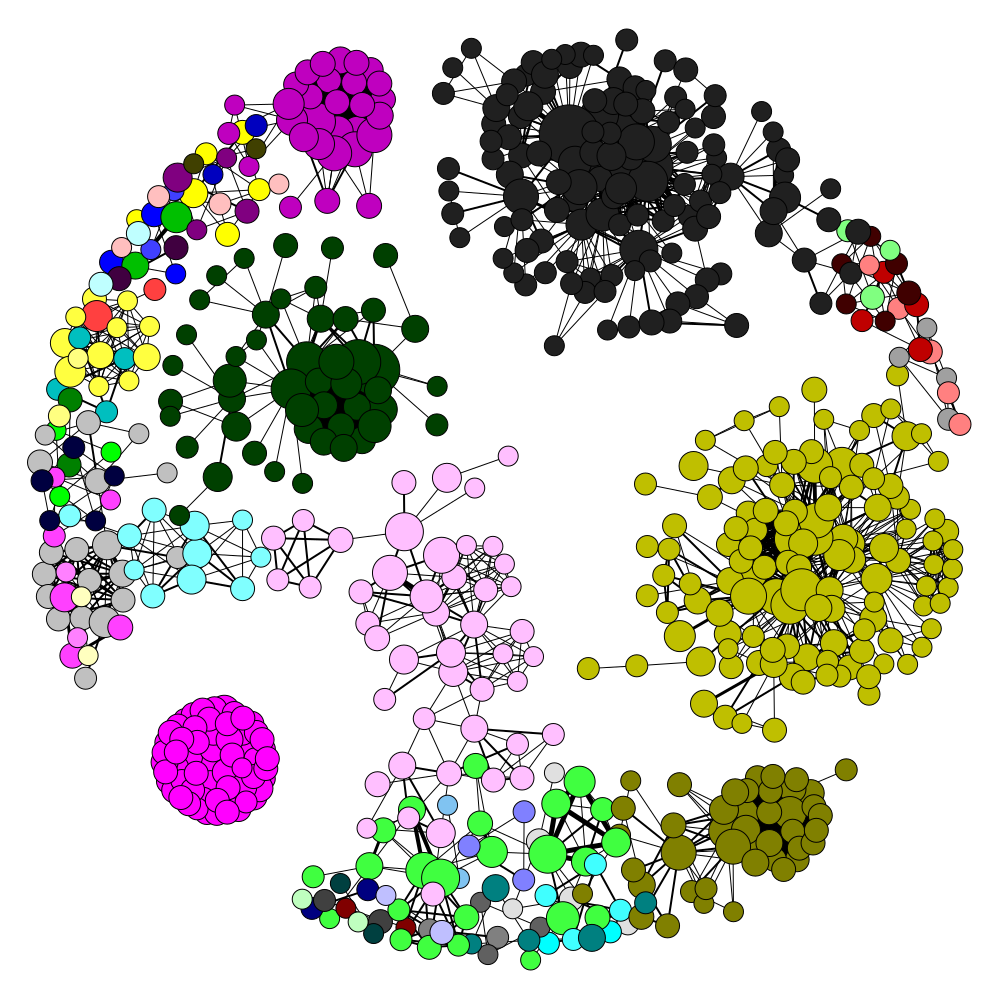
\includegraphics[width=13cm]{communities/researcher_a_cs}}
    \caption[Visualisation of the community structure within the \textit{Researcher-topic} network]{Visualisation of the community structure within the \textit{Researcher-topic} network constructed using the current (2010 to 2016) data set.}
    \label{fig:researcher_a_current_cs}
\end{figure}

\subsection{Evaluation}

Similarly to the \textit{Topic-grant} network, the \textit{Researcher-topic} network also underwent the evaluation phase and the results show that nodes within the same cluster have a higher similarity than nodes from different clusters. Table \ref{table:researcher_a_evaluation} presents the results of the evaluation phase carried out on the \textit{Researcher-topic} network constructed using the current (2010 to 2016) data set.

\begin{table}[htpb]
\centering
\caption[Dice and Jaccard similarity coefficients of node pairs within and between communities in the \textit{Researcher-topic} network constructed using the current (2010 to 2016) data set]{Dice and Jaccard similarity coefficients of node pairs within and between communities in the \textit{Researcher-topic} network constructed using the current (2010 to 2016) data set. Each node pair represents an edge which connects two nodes within the same community or in two different communities. \textit{IN} stands for within communities, while \textit{OUT} means between communities.}
\label{table:researcher_a_evaluation}
\begin{tabular}{r|r}
{} & \textbf{2010-2016}\\
\hline\\
Node pairs IN                  & {4273}\\
Node pairs OUT                 & {275}\\
Average Dice similarity IN     & {0.835}\\
Average Dice similarity OUT    & {0.405}\\
Difference between IN and OUT  & {0.430}\\
Average Jaccard similarity IN  & {0.779}\\
Average Jaccard similarity OUT & {0.273}\\
Difference between IN and OUT  & {0.506}\\
\end{tabular}
\end{table}

\subsection{Discussion}

The \textit{Researcher-grant} and \textit{Researcher-topic} networks represent two interpretations of the researcher data. This means a comparative analysis can be conducted comparing the two networks in terms of clustering.

\subsubsection{Comparison to Researcher-topic network}

The clustering results produced using both networks clearly indicate that the \textit{Researcher-topic}  network is the more rational and valuable interpretation of the researcher data, as expected prior to the creation process of the \textit{Researcher} networks.

In one hand, there is a network that consists of researchers and links between them symbolising a work collaboration between the two. As proved by the results, this is fairly rare in the academic world. Unless two researchers have a relationship, are part of the same institution or organisation or are located in the same city, it is hard to believe that they would collaborate on multiple occasions. Moreover, it is essential to note that there is a clear difference between collaborating on a government-funded grant and any other research project. Certain grants can last up to 7 years and at the end of the grant the researchers that worked on it will most probably not collaborative again for a lengthy period of time, if at all. In conclusion, the grant-based interpretation of the researcher data did not prove to be significantly valuable. However it did provide interesting insights into the progress of research and research funding over a 26-year long period.

On the other hand, there is a network that consists of researchers and links between them symbolising a shared research interest between the two. This type of connection between two researchers is not limited to a relationship, institution or organisation, or location. Only a shared research interest is required. In the academic world, this is very common as researchers from all over the world can connect and relate to each other through a common research field. The ideal result from such a network is a fairly low number of communities consisting of researchers that share an interest in a number of different topics. However, due to the large number of researchers, the number of identified communities turns out to be large and at the same time, sparse. That being said, this interpretation of the data is still a better option than the first, as it produces a more compelling clustering based on the researcher data available.
\chapter{\textsc{Discussion}}
\label{chapter:discussion}

In this chapter, the key results produced are summarised, and the limitations and improvements of the project are outlined, while the improvements are translated into future work, which is recommended.

\section{Summary of key results}

At the end of this thesis project, three key results were produced. Firstly, a rational, well-defined and balanced clustering of current and historical research topics was achieved. Secondly, a concrete work collaboration network between researchers was discovered, however, its clustering resulted in a substantial amount of communities which slightly diminished the extent of its analysis and its potential value.

Finally, an optimal solution composed of an edge weight and a community detection algorithm was identified. The optimal solution identified outperformed all other solutions considered in the comparison experiments. Furthermore, the key results produced represent the fulfilment of the objectives set at the start of the project.

Additionally, the impact of the results depends on who makes use of which results and how those results are used. Specifically, the identification of rational topic and researcher clusters is valuable to EPSRC as it represents a coherent way of clustering topics based on similarity and relatedness, a solution to a problem which currently exists.

Furthermore, the data analysis performed and the network visualisations produced represent invaluable insights into both the current and historical data. On the other hand, the identification of an optimal combination of edge weight and community detection algorithm as a result of the exhaustive experiments conducted, is more important to someone who wants to address a different but similar clustering problem as the one addressed in this project.

\section{Limitations}

Due to the short amount of time available, the analysis performed on the \textit{Researcher} networks is slightly limited when compared to the analysis of the \textit{Topic} networks, in terms of the quantity of data collected and the extent of the analysis. However, this was justified in the end, as the value and importance of the results produced during the analysis of the \textit{Researcher} networks was minimised, when compared to the results of the \textit{Topic} networks analysis.

\section{Improvements}

The potential improvements of the project solely concern the analysis carried out on the \textit{Researcher} networks, as additional data can be collected and analysed. By collecting additional data about the researchers such as their department and organisation, would enable the discovery of potential correlations between the way researchers are clustered and their department, organisation or location.

\section{Future work}

Any research project, this included, can be extended to include more data or further experiments or analysis. In this case, four possible ways of extending the work carried out were identified:

\begin{itemize}[noitemsep]
    \item Extending comparison experiments stage to include more community detection algorithms
    \item Extending the analysis of the \textit{Researcher} networks
        \item Incorporate further data as node and edge attributes of the networks
    \item Comparison to a study carried out within a different context e.g. citation networks
\end{itemize}

\noindent Firstly, the comparison experiments stage which is partially concerned with the identification of an optimal community detection algorithm for the data, can be extended to include additional community detection algorithms to the ones already considered. This study carried out experiments using all community detection algorithms provided by the iGraph network analysis package. However, other packages are available, and consist of algorithms which are not included in iGraph. Therefore, these algorithms could be implemented and Incorporated into the experiments in order to determine whether better clustering results than the ones produced by the \textit{Louvain} community detection algorithm can be achieved.

Secondly, the analysis of the \textit{Researcher} networks was restricted by the amount of time available. By nature, the \textit{Researcher} networks are less informative than the \textit{Topic} networks as topics can be easily identified by people without additional knowledge, while researchers are cannot unless those same people know the researchers or work within EPSRC. However, the \textit{EPSRC GoW} service provides substantial public data, which is partly used in this project, but not fully. Both grant and researcher records consist of additional information which is not used in this project within fields such as the \textit{Department}, \textit{Organisation} and \textit{Industrial Sector Classifications} of a grant or the \textit{Organisation} and \textit{Department} of a researcher. Incorporating additional data in the form of node and edge attributes within both the \textit{Topic} and \textit{Researcher} networks will increase the level of contextual information available and provide a guaranteed extension of the analysis scope.

Finally, another way of extending this work can involve a comparative analysis of the results produced in this project and the results of a study with a similar end goal but which aimed to solve a different kind of practical or scientific problem. For example, this could represent a study involving the analysis of a citation network constructed based on the citations within a significant number of research papers. The objective would be to cluster research papers together in the hope that they share a common subject and researcher topic clusters are revealed. A comparative study may result in valuable insights into potential correlations between the two result sets while, also help cement graph theory as an optimal and valuable solution to clustering problems in both real-world and scientific scenarios.
\chapter{\textsc{Conclusion}}
\label{chapter:conclusion}

In this project, graph theory was used as a novel approach to a real-world problem, involving the identification of topic and researcher clusters in publicly available data provided by EPSRC. The objective of the project was not only to provide a solution to the problem, but also to determine whether graph theory could provide the solution.

Furthermore, the problem that the project aims to solve was defined and extensive background information about EPSRC, the concept of modularity and community detection algorithms was provided. The state-of-the-art of the related topics was also reviewed. Additionally, the methods put into practice throughout every stage of the project were explained in detail.

The current and historical data collected from EPSRC was interpreted in a number of different ways and lead to several \textit{Topic} and \textit{Researcher} networks being constructed using both the current (2010 to 2016) and historical (1990 to 2000, 2000 to 2010) data sets. This was followed by an extensive comparison experiments on both current and historical data sets which aimed to identify an optimal edge weight and community detection algorithm that would result in a highly accurate and coherent clustering of topics and researchers. The candidates considered included three different interpretations of the edge weight attribute (\textit{unweighted}, \textit{weighted by normalised number of grants}, \textit{weighted by normalised value of grants}) and eight different community detection algorithms including \textit{Louvain}, \textit{Spinglass} and \textit{Fast Greedy}.

The comparative analysis resulted in a significant and valuable set of results. Firstly, edges \textit{weighted by the normalised number of grants} was determined as the optimal interpretation of the edge weight attribute due to its high modularity score and rational clustering produced. Secondly, the \textit{Louvain} method was "crowned" as the optimal community detection algorithm due to its high performance in the experiments and the well-defined nature of the community structure it identified. Finally, using the \textit{Topic-grant} and \textit{Researcher-topic} networks proved to be a better option than other network interpretations, as more cogent and balanced clusters of topics and researchers were produced.

This thesis, based on the knowledge available, represents the first approach of deploying graph theory in order to provide a solution to a real-world problem which at the moment, is specific to one organisation - EPSRC. With the data undergoing extensive experimental comparison, an evaluated solution featuring surprisingly high performance is identified and proposed.

In conclusion, this project represents clear evidence that the novel approach based on graph theory is of great value and, because it is not limited by any data set, it can be used to identify solutions to other real-world problems, perhaps the identification of topic communities within a network of newspaper articles.
\chapter{\textsc{Glossary}}
\label{chapter:glossary}

This glossary explains how the network naming convention was formulated while also specifying the long form of the abbreviations used in the thesis.

\section{Naming convention}

Throughout this thesis project, networks are mentioned using a standard naming convention, as follows:

\begin{center}
\underline{term1} dash \underline{term2} network
\end{center}

\noindent where:

\begin{itemize}[noitemsep]
    \item term1 means that \underline{nodes} represent \underline{term1} in the network
    \item term2 means that \underline{edges} represent \underline{term2} in the network
\end{itemize}

\noindent The standard naming convention is used to name the 4 networks constructed in this project, as follows:

\begin{itemize}[noitemsep]
    \item \textbf{Topic-grant network}, in which:
    \begin{itemize}[noitemsep]
        \item \underline{first term (topic)} means that nodes represent \underline{topics}
        \item \underline{second term (grant)} means that edges represent \underline{grants}
    \end{itemize}
    \item \textbf{Topic-researcher network}, in which:
    \begin{itemize}
        \item \underline{first term (topic)} means that nodes represent \underline{topics}
        \item \underline{second term (researcher)} means that edges represent \underline{researchers}
    \end{itemize}
    \item \textbf{Researcher-grant network}, in which:
    \begin{itemize}
        \item \underline{first term (researcher)} means that nodes represent \underline{researchers}
        \item \underline{second term (grant)} means that edges represent \underline{grants}
    \end{itemize}
    \item \textbf{Researcher-topic network}, in which:
    \begin{itemize}
        \item \underline{first term (researcher)} means that nodes represent \underline{researchers}
        \item \underline{second term (topic)} means that edges represent \underline{topics}
    \end{itemize}
\end{itemize}

\clearpage

\section{List of abbreviations}

A number of abbreviations are also used in the thesis report, particularly in the comparison experiments, and their long form is the following:

\begin{itemize}[noitemsep]
    \item \textbf{EPSRC} stands for \underline{\textbf{E}}ngineering and \underline{\textbf{P}}hysical \underline{\textbf{S}}ciences \underline{\textbf{R}}esearch \underline{\textbf{C}}ouncil
    \item \textbf{GoW} stands for \underline{\textbf{G}}rants \underline{\textbf{o}}n the \underline{\textbf{W}}eb
    \vspace{1em}
    \item \textbf{uw} stands for edge \underline{\textbf{u}}n\underline{\textbf{w}}eighted
    \item \textbf{wnn} stands for edge \underline{\textbf{w}}eighted by \underline{\textbf{n}}ormalized \underline{\textbf{n}}umber of grants
    \item \textbf{wnv} stands for edge \underline{\textbf{w}}eighted by \underline{\textbf{n}}ormalized \underline{\textbf{v}}alue of grants
    \vspace{1em}
    \item \textbf{SG} stands for \underline{\textbf{S}}pin\underline{\textbf{g}}lass community detection algorithm
    \item \textbf{LV} stands for \underline{\textbf{L}}ou\underline{\textbf{v}}ain community detection algorithm
    \item \textbf{FG} stands for \underline{\textbf{F}}ast \underline{\textbf{G}}reedy community detection algorithm
\end{itemize}
\phantomsection
% This line manually adds the Bibliography to the table of contents.
% The fact that \include is the last thing before this ensures that it
% is on a clear page, and adding it like this means that it doesn't
% get a chapter or appendix number.
\addcontentsline{toc}{chapter}{\textsc{References}}

\renewcommand{\bibname}{\textsc{References}}
% Actually generates your bibliography.
\bibliography{references/references.bib}

\phantomsection
\addcontentsline{toc}{chapter}{\textsc{Appendices}}
\renewcommand*{\arraystretch}{1.5}

\appendix

\chapter{Data Management Plan}
\label{appendix:data_management_plan}

A Research Data Management Plan was compiled and can be accessed at the following address:

\url{https://github.com/SergiuTripon/msc-thesis-na-epsrc/blob/master/documents/research-data-management-plan/pdf/research_data_management_plan.pdf}

\chapter{EPSRC grant data}
\label{appendix:epsrc_grant_data}

\begin{spacing}{0.9}
\begin{longtable}[r]{r|r|p{11.5cm}}
\caption[Topics clustered within each community and sub-community discovered by the optimal solution identified in the experiment on the \textit{Topic-grant} network constructed using the current (2010 to 2016) data set]{Topics clustered within each sub-community of Community 1 discovered by the optimal solution identified in the experiment on the \textit{Topic-grant} network constructed using the current (2010 to 2016) data set. \textbf{C1} stands for Community 1. Rows representing sub-communities are named using second-level labels (1.1, 1.2 and so on).}\\
\label{table:topic_a_current_clusters_appendix}
{} & {}\\
\hline
\endfirsthead
\caption[]{Continued from previous page.}\\
\hline
\endhead
\textbf{C1}
& \textbf{1.1} & {ageing: chemistry/biochemistry, analytical science, biomedical sciences}\\
& \textbf{1.2} & {biomaterials, med.instrument.device\& equip., biomechanics \& rehabilitation, medical imaging, biomedical neuroscience, novel industrial products, development (biosciences), systems neuroscience, drug formulation \& delivery, tissue engineering, mathematical \& statistic psych}\\
& \textbf{1.3} & {drug formulation \& delivery, tissue engineering, mathematical \& statistic psych, bioelectronic devices, medical science \& disease, bioinformatics, microbiology, cells, population ecology, complex fluids \& soft solids, theoretical biology, genomics}\\
& \textbf{1.4} & {biological \& medicinal chem., protein chemistry, catalysis \& enzymology, protein folding / misfolding, chemical biology, structural biology}\\
\hline
\textbf{C2}
& \textbf{2.1} & {artificial intelligence, information \& knowledge mgmt, behavioural \& experimental eco, intelligent measurement sys., comput./corpus linguistics, international law, computational linguistics, marketing, criminal law \& criminology, psychology, criminology, science \& technology studies, governance, social policy}\\
& \textbf{2.2} & {cognitive psychology, image \& vision computing, cognitive science appl. in ict, mental health, composition, music \& acoustic technology, design processes, musical performance, developmental psychology, new \& emerging comp. paradigms, human communication in ict, robotics \& autonomy, human-computer interactions, vision \& senses - ict appl.}\\
& \textbf{2.3} & {macroeconomics, political geography}\\
& \textbf{2.4} & {animal behaviour, networks \& distributed systems, computer sys. \& architecture, organisational studies, data handling \& storage, parallel computing, digital signal processing, rf \& microwave technology, fundamentals of computing, social psychology, industrial-org/occupational, software engineering, international relations theory, system on chip, knowledge management, vlsi design, modelling \& simul. of it sys.}\\
& \textbf{2.5} & {applied arts htp, mobile computing, computer graphics \& visual., multimedia, design engineering, new media/web-based studies, digital art \& design, product design, digital arts htp, social anthropology, manufact. business strategy, social theory, media \& communication studies, time-based media htp}\\
\hline
\textbf{C3}
& \textbf{3.1} & {acoustics, fluid dynamics, aerodynamics, heat \& mass transfer, assess/remediate contamination, microsystems, bioenergy, multiphase flow, coal technology, pollution, combustion, power sys man, prot \& control, control engineering, power systems plant, development geography, rheology, earth engineering, separation processes, electric motor \& drive systems, underwater engineering, energy - conventional, wind power, energy - marine \& hydropower}\\
& \textbf{3.2} & {biochemical engineering, macro-molecular delivery, bioprocess engineering, manufact. enterprise ops\& mgmt, design of process systems, manufacturing machine \& plant, food processing, particle technology, food structure/composition, protein engineering, intelligent \& expert systems}\\
& \textbf{3.3} & {asymmetric chemistry, gas \& solution phase reactions, carbohydrate chemistry, materials characterisation, catalysis \& applied catalysis, materials processing, chemical structure, materials synthesis \& growth, chemical synthetic methodology, physical organic chemistry, co-ordination chemistry, plant physiology, electrochemical science \& eng., plant responses to environment, electromagnetics, reactor engineering, evolution \& populations, surfaces \& interfaces}\\
& \textbf{3.4} & {carbon capture \& storage, instrumentation eng. \& dev., diamond light source, materials testing \& eng., energy storage, mech. \& fluid power transmiss., eng. dynamics \& tribology, oil \& gas extraction, fuel cell technologies}\\
& \textbf{3.5} & {research approaches, synthetic biology}\\
\hline
\textbf{C4}
& \textbf{4.1} & {mathematical aspects of or, microeconomic theory}\\
& \textbf{4.2} & {algebra \& geometry, mathematical physics, continuum mechanics, non-linear systems mathematics, logic \& combinatorics, numerical analysis, mathematical analysis, statistics \& appl. probability}\\
\hline
\textbf{C5}
& \textbf{5.1} & {complexity science, management \& business studies, economics, social stats., comp. \& methods, education, sociology, environmental planning, sustainable energy networks, human geography (general), urban \& land management}\\
& \textbf{5.2} & {animal organisms, energy - nuclear, climate \& climate change, land - ocean interactions, coastal \& waterway engineering, regional \& extreme weather, earth \& environmental}\\
& \textbf{5.3} & {building ops \& management, pavement engineering, civil engineering materials, structural engineering, construction ops \& management, sustainable energy vectors, energy efficiency, waste management, environment \& health, waste minimisation, environmental economics, water engineering}\\
& \textbf{5.4} & {geohazards, survey \& monitoring, ground engineering, transport ops \& management, soil science}\\
\hline
\textbf{C6}
& \textbf{6.1} & {design \& testing technology, optical devices \& subsystems, displays, optical phenomena, electronic devices \& subsys., optoelect. devices \& circuits, lasers \& optics, power electronics, optical communications}\\
& \textbf{6.2} & {biological membranes, magnetism/magnetic phenomena, biophysics, solar technology, condensed matter physics, tools for the biosciences, high performance computing}\\
& \textbf{6.3} & {computational methods \& tools, plasmas - laser \& fusion, fusion, plasmas - technological}\\
& \textbf{6.4} & {atoms \& ions, quantum fluids \& solids, cold atomic species, quantum optics \& information, light-matter interactions, scattering \& spectroscopy}
\end{longtable}
\end{spacing}

\clearpage

\begin{spacing}{0.9}
\begin{longtable}[r]{r|r|p{11.5cm}}
\caption[Topics clustered within each community and sub-community discovered in the \textit{Topic-grant} network constructed using the historical (2000 to 2010) data set]{Topics clustered within each community and sub-community discovered as a result of applying the Louvain community detection algorithm to the \textit{Topic-grant} network constructed using the historical (2000 to 2010) data set. Six of the row names are abbreviated: \textbf{C1} stands for Community 1, \textbf{C2} for Community 2 and so on. Rows representing sub-communities of a community are named using second-level labels (1.1, 1.2, 2.1, 2.2 and so on).}\\
\label{table:topic_a_historical1_clusters_appendix}
{} & {}\\
\hline
\endfirsthead
\caption[]{Continued from previous page.}\\
\hline
\endhead
\textbf{C1}
& \textbf{1.1} & {analytical science, co-ordination chemistry, asymmetric chemistry, combinatorial chemistry, biological \& medicinal chem., electrochemical science \& eng., carbohydrate chemistry, mantle \& core processes, catalysis \& applied catalysis, physical organic chemistry, chemical synthetic methodology, reactor engineering}\\
& \textbf{1.2} & {astron. \& space sci. technol., light-matter interactions, atoms \& ions, magnetism/magnetic phenomena, catalysis \& enzymology, nuclear structure, chemical structure, optical phenomena, cold atomic species, plasmas - laser \& fusion, condensed matter physics, plasmas - technological, galactic \& interstellar astron, quantum fluids \& solids, gas \& solution phase reactions, quantum optics \& information, high performance computing, scattering \& spectroscopy, lasers \& optics, surfaces \& interfaces}\\
& \textbf{1.3} & {bioelectronic devices, medical science \& disease, electronic devices \& subsys., microsystems, instrumentation eng. \& dev., musculoskeletal system, materials characterisation, optical communications, materials processing, optical devices \& subsystems, materials synthesis \& growth, optoelect. devices \& circuits}\\
& \textbf{1.4} & {biological membranes, chemical biology, bionanoscience, protein chemistry, bionanotechnology, protein folding / misfolding, biophysics, structural biology}\\
& \textbf{1.5} & {biomaterials, genomics, bioprocess engineering, particle technology, cells, rheology, complex fluids \& soft solids, separation processes, development (biosciences), stem cell biology, drug formulation \& delivery, synthetic biology, food processing, tissue engineering, food structure/composition}\\
\hline
\textbf{C2}
& \textbf{2.1} & {aerodynamics, manufact. business strategy, control engineering, manufact. enterprise ops\& mgmt, design \& testing technology, manufacturing machine \& plant, electromagnetics
}\\
& \textbf{2.2} & {algebra \& geometry, mathematical aspects of or, animal \& human physiology, mathematical physics, complexity science, multiphase flow, continuum mechanics, non-linear systems mathematics, design of process systems, numerical analysis, evolution \& populations, population ecology, fluid dynamics, statistics \& appl. probability, logic \& combinatorics, theoretical biology, mathematical analysis, upper atmos process \& geospace}\\
& \textbf{2.3} & {acoustics, materials testing \& eng., assess/remediate contamination, mech. \& fluid power transmiss., building ops \& management, pavement engineering, civil engineering materials, structural engineering, coastal \& waterway engineering, transport ops \& management, construction ops \& management, urban \& land management, design engineering, waste management, eng. dynamics \& tribology, waste minimisation, ground engineering, water engineering}\\
\hline
\textbf{C3}
& \textbf{3.1} & {bioenergy, fuel cell technologies, carbon capture \& storage, fusion, electric motor \& drive systems, power sys man, prot \& control, energy - conventional, solar technology, energy - nuclear, sustainable energy networks, energy efficiency, sustainable energy vectors, energy storage, wind power}\\
& \textbf{3.2} & {microbiology, power electronics}\\
& \textbf{3.3} & {coal technology, mining \& minerals extraction, combustion, safety \& reliability of plant, heat \& mass transfer}\\
& \textbf{3.4} & {energy - marine \& hydropower, power systems plant, oil \& gas extraction, underwater engineering}\\
\hline
\textbf{C4}
& \textbf{4.1} & {crop science, soil science}\\
\hline
\textbf{C5}
& \textbf{5.1} & {artificial intelligence, languages \& linguistics, bioinformatics, modelling \& simul. of it sys., biomechanics \& rehabilitation, new \& emerging comp. paradigms, biomedical neuroscience, parallel computing, cognitive science appl. in ict, rf \& microwave technology, computer sys. \& architecture, robotics \& autonomy, digital signal processing, software engineering, fundamentals of computing, system on chip, image \& vision computing, vision \& senses - ict appl., intelligent measurement sys., vlsi design}\\
& \textbf{5.2} & {applied arts htp, media \& communication studies, cultural history, mental health, design htp, mobile computing, design processes, multimedia, digital art \& design, music \& acoustic technology, digital arts htp, networks \& distributed systems, economic \& social history, new media/web-based studies, economics, policy, arts mgmt \& creat ind, intelligent \& expert systems, product design, language acquisition, publishing, language training/educational, social stats., comp. \& methods, management \& business studies, sociology, med.instrument.device\& equip.}\\
& \textbf{5.3} & {cultural studies \& pop culture, pollution, displays, psychology, information \& knowledge mgmt}\\
& \textbf{5.4} & {accelerator r\&d, escience, agricultural systems, human communication in ict, applied linguistics, human geography, archaeology of literate soc., human-computer interactions, comput./corpus linguistics, interpreting \& translation, computer graphics \& visual., medical imaging, drama \& theatre - other, psycholinguistics, education, science-based archaeology, environmental informatics, sociolinguistics, environmental planning}
\end{longtable}
\end{spacing}

\clearpage

\begin{spacing}{0.9}
\begin{longtable}[r]{r|r|p{11.5cm}}
\caption[Topics clustered within each community and sub-community discovered in the \textit{Topic-grant} network constructed using the historical (1990 to 2000) data set]{Topics clustered within each community and sub-community discovered as a result of applying the Louvain community detection algorithm to the \textit{Topic-grant} network constructed using the historical (1990 to 2000) data set. Six of the row names are abbreviated: \textbf{C1} stands for Community 1, \textbf{C2} for Community 2 and so on. Rows representing sub-communities of a community are named using second-level labels (1.1, 1.2, 2.1, 2.2 and so on).}\\
\label{table:topic_a_historical2_clusters_appendix}
{} & {}\\
\hline
\endfirsthead
\caption[]{Continued from previous page.}\\
\hline
\endhead
\textbf{C1}
& \textbf{1.1} & {acoustics, intelligent measurement sys., aerodynamics}\\
& \textbf{1.2} & {coal technology, energy - conventional, combustion, safety \& reliability of plant}\\
& \textbf{1.3} & {bioprocess engineering, heat \& mass transfer, cells, multiphase flow, complex fluids \& soft solids, particle technology, design of process systems, reactor engineering, fluid dynamics, rheology}\\
& \textbf{1.4} & {building ops \& management, transport ops \& management, computer graphics \& visual., urban \& land management, energy efficiency, wind power, intelligent \& expert systems}\\
& \textbf{1.5} & {bioenergy, waste minimisation, waste management, water engineering}\\
\hline
\textbf{C2}
& \textbf{2.1} & {condensed matter physics, materials synthesis \& growth, magnetism/magnetic phenomena, quantum fluids \& solids, materials characterisation, solar technology, materials processing, sustainable energy networks}\\
& \textbf{2.2} & {displays, optoelect. devices \& circuits, electronic devices \& subsys., power electronics, microsystems, system on chip, optical communications, vlsi design, optical devices \& subsystems}\\
& \textbf{2.3} & {atoms \& ions, optical phenomena, cold atomic species, plasmas - laser \& fusion, lasers \& optics, quantum optics \& information, light-matter interactions, scattering \& spectroscopy}\\
\hline
\textbf{C3}
& \textbf{3.1} & {development (biosciences), modelling \& simul. of it sys., drug formulation \& delivery, theoretical biology}\\
& \textbf{3.2} & {algebra \& geometry, mathematical analysis, fundamentals of computing, mathematical physics}\\
& \textbf{3.3} & {continuum mechanics, numerical analysis, logic \& combinatorics, parallel computing, mathematical aspects of or, population ecology, medical science \& disease, statistics \& appl. probability, non-linear systems mathematics}\\
\hline
\textbf{C4}
& \textbf{4.1} & {control engineering, manufacturing machine \& plant, electric motor \& drive systems, mech. \& fluid power transmiss.}\\
& \textbf{4.2} & {bioelectronic devices, mobile computing, cognitive science appl. in ict, multimedia, digital signal processing, networks \& distributed systems, electromagnetics, rf \& microwave technology, human communication in ict, vision \& senses - ict appl., human-computer interactions}\\
& \textbf{4.3} & {assess/remediate contamination, ground engineering, civil engineering materials, materials testing \& eng., coastal \& waterway engineering, music \& acoustic technology, energy - nuclear, oil \& gas extraction, eng. dynamics \& tribology, pavement engineering}\\
& \textbf{4.4} & {construction ops \& management, manufact. business strategy, design \& testing technology, manufact. enterprise ops\& mgmt, design engineering, nuclear structure, design processes, software engineering, information \& knowledge mgmt}\\
& \textbf{4.5} & {artificial intelligence, tools for the biosciences, image \& vision computing, underwater engineering,robotics \& autonomy}\\
\hline
\textbf{C5}
& \textbf{5.1} & {biological \& medicinal chem., chemical synthetic methodology, catalysis \& enzymology, co-ordination chemistry, chemical biology, gas \& solution phase reactions, chemical structure, physical organic chemistry}\\
& \textbf{5.2} & {asymmetric chemistry, catalysis \& applied catalysis, carbohydrate chemistry, combinatorial chemistry}\\
& \textbf{5.3} & {analytical science, plasmas - technological, instrumentation eng. \& dev., surfaces \& interfaces}\\
& \textbf{5.4} & {biomaterials, power systems plant, med.instrument.device\& equip., tissue engineering, power sys man, prot \& control}\\
& \textbf{5.5} & {electrochemical science \& eng., mining \& minerals extraction, energy storage, separation processes, fuel cell technologies, sustainable energy vectors}
\end{longtable}
\end{spacing}

\clearpage

\begin{spacing}{0.9}
\begin{longtable}[r]{r|r|p{11.5cm}}
\caption[Topics clustered within each community and sub-community discovered in the \textit{Topic-researcher} network constructed using the current (2010 to 2016) data set]{Topics clustered within each community and sub-community discovered as a result of applying the Louvain community detection algorithm to the \textit{Topic-researcher} network constructed using the current (2010 to 2016) data set. Six of the row names are abbreviated: \textbf{C1} stands for Community 1, \textbf{C2} for Community 2 and so on. Rows representing sub-communities of a community are named using second-level labels (1.1, 1.2, 2.1, 2.2 and so on).}\\
\label{table:topic_b_current_clusters_appendix}
{} & {}\\
\hline
\endfirsthead
\caption[]{Continued from previous page.}\\
\hline
\endhead
\textbf{C1}
& \textbf{1.1} & {building ops \& management, manufact. business strategy, civil engineering materials, pavement engineering, construction ops \& management, robotics \& autonomy, design \& testing technology, soil science, earth engineering, structural engineering, environmental economics, survey \& monitoring, geohazards, waste management, ground engineering, wind power}\\
& \textbf{1.2} & {animal organisms, environment \& health, climate \& climate change, food processing, coastal \& waterway engineering, land - ocean interactions, earth \& environmental, water engineering, energy - marine \& hydropower}\\
& \textbf{1.3} & {aerodynamics, intelligent measurement sys., complexity science, management \& business studies, education, social stats., comp. \& methods, energy efficiency, sociology, environmental planning, sustainable energy networks, human geography (general), transport ops \& management, intelligent \& expert systems, urban \& land management}\\
\hline
\textbf{C2}
& \textbf{2.1} & {cognitive psychology, information \& knowledge mgmt, comput./corpus linguistics, marketing, computational linguistics, mental health, design processes, mobile computing, developmental psychology, psychology, human communication in ict, social theory, human-computer interactions}\\
& \textbf{2.2} & {behavioural \& experimental eco, mathematical \& statistic psych, criminal law \& criminology, media \& communication studies, criminology, modelling \& simul. of it sys., governance, organisational studies, international law, social policy, knowledge management, social psychology}\\
& \textbf{2.3} & {bioinformatics, design engineering, biomedical neuroscience, new \& emerging comp. paradigms, cognitive science appl. in ict, research approaches, control engineering, vision \& senses - ict appl.}\\
& \textbf{2.4} & {computer sys. \& architecture, parallel computing, data handling \& storage, political geography, fundamentals of computing, product design, industrial-org/occupational, software engineering, international relations theory, underwater engineering, networks \& distributed systems, vlsi design}\\
& \textbf{2.5} & {animal behaviour, macroeconomics, applied arts htp, multimedia, artificial intelligence, music \& acoustic technology, composition, musical performance, computer graphics \& visual., new media/web-based studies, digital art \& design, science \& technology studies, digital arts htp, social anthropology, digital signal processing, time-based media htp, image \& vision computing}\\
\hline
\textbf{C3}
& \textbf{3.1} & {genomics, theoretical biology}\\
& \textbf{2.2} & {algebra \& geometry, non-linear systems mathematics, continuum mechanics, numerical analysis, logic \& combinatorics, regional \& extreme weather, mathematical analysis, statistics \& appl. probability, mathematical physics}\\
& \textbf{2.3} & {acoustics, microeconomic theory, mathematical aspects of or, rheology}\\
\hline
\textbf{C4}
& \textbf{4.1} & {ageing: chemistry/biochemistry, magnetism/magnetic phenomena, analytical science, materials characterisation, atoms \& ions, materials synthesis \& growth, bioelectronic devices, optical communications, biological membranes, optical devices \& subsystems, biomedical sciences, optical phenomena, bionanoscience, optoelect. devices \& circuits, biophysics, plant physiology, carbohydrate chemistry, plant responses to environment, chemical structure, pollution, cold atomic species, quantum fluids \& solids, complex fluids \& soft solids, quantum optics \& information, condensed matter physics, rf \& microwave technology, displays, scattering \& spectroscopy, electronic devices \& subsys., solar technology, evolution \& populations, surfaces \& interfaces, high performance computing, system on chip, lasers \& optics, tools for the biosciences, light-matter interactions}\\
& \textbf{4.2} & {accelerator r\&d, fuel cell technologies, assess/remediate contamination, fusion, bioenergy, instrumentation eng. \& dev., carbon capture \& storage, manufact. enterprise ops\& mgmt, coal technology, manufacturing machine \& plant, combustion, materials processing, computational methods \& tools, materials testing \& eng., development geography, mech. \& fluid power transmiss., economics, oil \& gas extraction, electric motor \& drive systems, plasmas - laser \& fusion, electromagnetics, plasmas - technological, energy - conventional, power sys man, prot \& control, energy - nuclear, power systems plant, energy storage, sustainable energy vectors, eng. dynamics \& tribology, waste minimisation, food structure/composition}\\
& \textbf{4.3} & {asymmetric chemistry, gas \& solution phase reactions, biochemical engineering, heat \& mass transfer, bioprocess engineering, macro-molecular delivery, catalysis \& applied catalysis, microsystems, chemical biology, multiphase flow, chemical synthetic methodology, particle technology, co-ordination chemistry, physical organic chemistry, design of process systems, protein engineering, diamond light source, reactor engineering, electrochemical science \& eng., separation processes, fluid dynamics, synthetic biology}\\
& \textbf{4.4} & {biological \& medicinal chem., microbiology, biomaterials, novel industrial products, biomechanics \& rehabilitation, population ecology, catalysis \& enzymology, power electronics, cells, protein chemistry, development (biosciences), protein folding / misfolding, drug formulation \& delivery, structural biology, med.instrument.device\& equip., systems neuroscience, medical imaging, tissue engineering, medical science \& disease}\\
\end{longtable}
\end{spacing}
\chapter{Source Code}
\label{appendix:code}

\definecolor{dkgreen}{rgb}{0,0.6,0}
\definecolor{gray}{rgb}{0.5,0.5,0.5}
\definecolor{mauve}{rgb}{0.58,0,0.82}

\lstdefinestyle{Python}{frame=tb,
  language=Python,
  aboveskip=3mm,
  belowskip=3mm,
  showstringspaces=false,
  columns=flexible,
  basicstyle={\small\ttfamily},
  numbers=none,
  numberstyle=\tiny\color{gray},
  keywordstyle=\color{blue},
  commentstyle=\color{dkgreen},
  stringstyle=\color{mauve},
  breaklines=true,
  breakatwhitespace=true,
  tabsize=3
}

\lstdefinestyle{Bash}{frame=tb,
  language=bash,
  basicstyle=\small\ttfamily,
  showstringspaces=false,
  commentstyle=\color{red},
  keywordstyle=\color{blue}
}

During this project, source code was written in Python and Bash and stored within \textbf{12 files (6,123 lines)}, as follows:

\begin{enumerate}[noitemsep, label*=\arabic*.]
    \item \textbf{Data collection (2,541 lines)}
\begin{enumerate}[label*=\arabic*.]
    \item \textbf{download.sh (153 lines)}, written to download grant and research records from the \textit{EPSRC GoW service}
    \item \textbf{extract.py (964 lines)}, written to extract information from the downloaded data
    \item \textbf{link.py (844 lines)}, written to establish the links between the topics and researchers
    \item \textbf{make.py (414 lines)}, written to create the \textit{Topic} and \textit{Researcher networks}
    \item \textbf{run.py (35 lines)}, written to run the \textit{extract.py}, \textit{link.py}, \textit{make.py} functions from one central file
    \item \textbf{check.sh (131 lines)}, written to ensure correct file creation
\end{enumerate}
    \item \textbf{Network analysis (3,582 lines)}
\begin{enumerate}[label*=\arabic*.]
    \item \textbf{network.py (711 lines)}, written to analyse the network
    \item \textbf{communities.py (598 lines)}, written to analyse the communities within the network
    \item \textbf{sub\_communities.py (423 lines)}, written to analyse the sub-communities in each community within the network
    \item \textbf{analysis.py (1,176 lines)}, written to bind the \textit{network.py}, \textit{communities.py}, \textit{sub\_communities.py} functions together in one central file
    \item \textbf{evaluation.py (173 lines)} written to evaluate the community structure identified
    \item \textbf{clean.sh (501 lines)}, written to delete multiple files from specific folders
\end{enumerate}
\end{enumerate}

\section{Source code location}

The source code is stored in a GitHub repository located at the following web address:

\url{https://github.com/SergiuTripon/msc-thesis-na-epsrc}

\section{Running the source code}

\textbf{Note: In order to run the source code, an virtual environment installation is required. The code is written in Python 3.5. The packages used in the project are listed in the \textit{requirements.txt} file and can be install using \textit{pip}}.

\vspace{1em}

\noindent Running the network analysis is achieved by running the \textit{analysis.py} file with the desired parameters (\textbf{-n} requires network (topic or researcher), \textbf{-i} requires interpretation (grants, researchers or topics), \textbf{-d} requires data set (1990-2000, 2000-2010, 2010-2016)), following the steps below:

\begin{lstlisting}[style=Bash]
# activate virtual environment
$ source venv/bin/activate

# navigate to analysis source folder
$ cd msc-thesis-na-epsrc/analysis/src/

# analyse topic (grants as edges, 2010-2016)
$ python analysis.py -n topic -i grants -d 2010-2016
# analyse topic (grants as edges, 2000-2010)
$ python analysis.py -n topic -i grants -d 2000-2010
# analyse topic (grants as edges, 1990-2000)
$ python analysis.py -n topic -i grants -d 1990-2000

# analyse topic (researchers as edges, 2010-2016)
$ python analysis.py -n topic -i researchers -d 2010-2016
# analyse topic (researchers as edges, 2000-2010)
$ python analysis.py -n topic -i researchers -d 2000-2010
# analyse topic (researchers as edges, 1990-2000)
$ python analysis.py -n topic -i researchers -d 1990-2000

# analyse researcher (grants as edges, 2010-2016)
$ python analysis.py -n topic -i grants -d 2010-2016
# analyse researcher (researchers as edges, 2000-2010)
$ python analysis.py -n topic -i grants -d 2000-2010
# analyse researcher (researchers as edges, 1990-2000)
$ python analysis.py -n topic -i grants -d 1990-2000

# analyse researcher (topics as edges, 2010-2016)
$ python analysis.py -n topic -i topics -d 2010-2016
# analyse researcher (topics as edges, 2000-2010)
$ python analysis.py -n topic -i topics -d 2000-2010
# analyse researcher (topics as edges, 1990-2000)
$ python analysis.py -n topic -i topics -d 1990-2000
\end{lstlisting}

\section{GitHub Wiki}

A GitHub Wiki was created to accompany this project and is located at the following web address: 

\url{https://github.com/SergiuTripon/msc-thesis-na-epsrc/wiki}

\noindent \textbf{Note: The information on the GitHub Wiki may be out-of-date}.

\section{Code snippets}

This section presents two code snippets which are considered particularly important. The first one achieves the contrast between grants as edges and grant records, while the second normalises the values of the node and edge attributes.

\clearpage

\subsection{Contrast between grants as edges and grant records}

This snippet of code was written in order to convert edges within the network in grants. Moreover, it calculates the number and value of grants within communities, between communities and within the entire network. Achieving this was extremely beneficial as it enabled the analysis of research trend and funding on the current (2010 to 2016) and historical (1990 to 2000, 2000 to 2010) data sets.

\begin{lstlisting}[caption={Code snippet showing function written to turn edges into grants and calculate the number and value of grants within network and communities and between communities.}\label{listing:turn_edges_into_grants}, style=Python]
# turns edges into grants
def turn_edges_into_grants(community, edge_type, method, count1, path):

    # variable to split path
    path_split = path.split('/', 3)

    # variable to hold temporary path
    path_temp = ''

    # if split path equals to current
    if path_split[1] == 'current':
        # set temporary path
        path_temp = '{}'.format(path_split[1])
    # if split path equals to past
    elif path_split[1] == 'past':
        # set temporary path
        path_temp = '{}/{}'.format(path_split[1], path_split[2])

    # variable to hold input file
    input_file = open(r'../../network-maker/output/grants/'
    '{}/info/grant_{}.pkl'.format(path_temp, path_split[0]), 'rb')
    # load data structure from file
    grant_entities = load(input_file)
    # close input file
    input_file.close()

    # variable to hold entity links
    entity_links = [[community.vs['label'][edge.source], community.vs['label'][edge.target]]
                    for edge in community.es()]

    # variable to hold grants
    grants = OrderedDict()

    # if split path equals to topics
    if path_split[0] == 'topics':

        # set grants
        grants = OrderedDict((ref, attr[1]) for entity_link in entity_links for ref, attr in grant_entities.items()
                             if entity_link[0] and entity_link[1] in attr[0])

    # if split path equals to researchers
    elif path_split[0] == 'researchers':

        # set grants
        grants = OrderedDict((ref, attr[1]) for entity_link in entity_links for ref, attr in grant_entities.items()
                             if entity_link[0] and entity_link[1] in [researcher[0] for researcher in attr[0]])

    # variable to hold number
    number = len([ref for ref in grants.keys()])

    # set locale to Great Britain
    setlocale(LC_ALL, 'en_GB.utf8')

    # variable to hold value
    value = sum([attr for attr in grants.values()])

    # variable to hold output file
    output_file = open('../../data/networks/{}/communities/txt/{}/{}/'
                       'grants.txt'.format(path, edge_type, method), mode='a')

    # if count1 is equal to 1
    if count1 == 1:

        # write header to file
        output_file.write('> Number and value of grants in each community\n\n')

        # write grant number and value to file
        output_file.write('- Community {}:    {:>4d} {}\n'.format(count1, number, currency(value, grouping=True)))

    # if count1 is not equal to 1
    else:

        # write grant number and value to file
        output_file.write('- Community {}:    {:>4d} {}\n'.format(count1, number, currency(value, grouping=True)))

    # return number and value
    return grants, number, value
\end{lstlisting}

\subsection{Normalisation of node and edge attribute values}

This code snippet was written in order to normalise the values of the node and edge attributes. The value of grants attribute, in particular, consisted of very large values, up to 7 digits. By normalising the values of the node and edge attributes, working with such large values was avoided and, therefore, the development, analysis and visualisation process was improved.

\begin{lstlisting}[caption={Code snippet showing function written to normalise the values of the node and edge attributes.}\label{listing:norm_vals}, style=Python]
# normalises values
def norm_vals(vals, new_min, new_max):

    # variable to hold old minimum and maximum
    old_min, old_max = min(vals), max(vals)
    # variable to hold old and new range
    old_range, new_range = old_max - old_min, new_max - new_min

    int_vals = [int(val) for val in vals]

    # variable to hold new values
    new_vals = [round((((val - old_min) * new_range / old_range) + new_min), 0) for val in int_vals]

    # return new values
    return new_vals
\end{lstlisting}

\chapter{Supplementary material}
\label{appendix:supplementary_material}

Additionally to the appendix in the thesis report, a 1095-page document of supplementary material was also produced and can be accessed either in the submission or at the following web address:

\url{https://github.com/SergiuTripon/msc-thesis-na-epsrc/blob/master/documents/supplementary-material/15110029_sergiu_tripon_supplementary_material.pdf}
%\phantomsection
\addcontentsline{toc}{chapter}{\textsc{Supplementary material}}
\renewcommand*{\arraystretch}{1.4}

\chapter{EPSRC grant data}
\label{appendix:epsrc_grant_data}

\section{Networks of Topics}

\subsection{Topic-grant network}

\begin{spacing}{0.9}
\begin{longtable}[c]{>{\raggedleft\arraybackslash}m{1cm}|>{\raggedleft\arraybackslash}m{10cm}}
\caption[Topics in the current (2010-2016) data set that are not in the historical (2000 to 2010) data set]{Topics in the current (2010-2016) data set that are not in the historical (2000 to 2010) data set used to construct the \textit{Topic-grant} network.}\\
\label{table:topic_a_comparison1_appendix}
\textbf{No.} & \textbf{Topics in 2010-2016 that are not in 2000 to 2010}\\
\hline
\endfirsthead
\caption[]{Continued from previous page.}\\
\textbf{No.} & \textbf{Topics in 2010-2016 that are not in 2000 to 2010}\\
\hline
\endhead
{1} & {animal organisms}\\
{2} & {behavioural \& experimental eco}\\
{3} & {criminal law \& criminology}\\
{4} & {criminology}\\
{5} & {industrial-org/occupational}\\
{6} & {political geography}\\
{7} & {ageing: chemistry/biochemistry}\\
{8} & {animal behaviour}\\
{9} & {biochemical engineering}\\
{10} & {biomedical sciences}\\
{11} & {climate \& climate change}\\
{12} & {cognitive psychology}\\
{13} & {composition}\\
{14} & {computational linguistics}\\
{15} & {computational methods \& tools}\\
{16} & {data handling \& storage}\\
{17} & {development geography}\\
{18} & {developmental psychology}\\
{19} & {diamond light source}\\
{20} & {earth \& environmental}\\
{21} & {earth engineering}\\
{22} & {environment \& health}\\
{23} & {environmental economics}\\
{24} & {geohazards}\\
{25} & {governance}\\
{26} & {human geography (general)}\\
{27} & {international law}\\
{28} & {international relations theory}\\
{29} & {knowledge management}\\
{30} & {land - ocean interactions}\\
{31} & {macro-molecular delivery}\\
{32} & {macroeconomics}\\
{33} & {marketing}\\
{34} & {mathematical \& statistic psych}\\
{35} & {microeconomic theory}\\
{36} & {musical performance}\\
{37} & {novel industrial products}\\
{38} & {organisational studies}\\
{39} & {plant physiology}\\
{40} & {plant responses to environment}\\
{41} & {protein engineering}\\
{42} & {regional \& extreme weather}\\
{43} & {research approaches}\\
{44} & {science \& technology studies}\\
{45} & {social anthropology}\\
{46} & {social policy}\\
{47} & {social psychology}\\
{48} & {social theory}\\
{49} & {survey \& monitoring}\\
{50} & {systems neuroscience}\\
{51} & {time-based media htp}
\end{longtable}
\end{spacing}

\clearpage

\begin{spacing}{0.9}
\begin{longtable}[c]{>{\raggedleft\arraybackslash}m{1cm}|>{\raggedleft\arraybackslash}m{10cm}}
\caption[Topics in the historical (2000 to 2010) data set that are not in the current (2010-2016) data set]{Topics in the historical (2000 to 2010) data set that are not in the current (2010-2016) data set used to construct the \textit{Topic-grant} network.}\\
\label{table:topic_a_comparison2_appendix}
\textbf{No.} & \textbf{Topics in 2000 to 2010 that are not in 2010-2016}\\
\hline
\endfirsthead
\caption[]{Continued from previous page.}\\
\textbf{No.} & \textbf{Topics in 2000 to 2010 that are not in 2010-2016}\\
\hline
\endhead
{1} & {animal \& human physiology}\\
{2} & {astron. \& space sci. technol.}\\
{3} & {cultural history}\\
{4} & {cultural studies \& pop culture}\\
{5} & {interpreting \& translation}\\
{6} & {publishing}\\
{7} & {accelerator r\&d}\\
{8} & {agricultural systems}\\
{9} & {applied linguistics}\\
{10} & {archaeology of literate soc.}\\
{11} & {bionanoscience}\\
{12} & {bionanotechnology}\\
{13} & {cell cycle}\\
{14} & {combinatorial chemistry}\\
{15} & {crop science}\\
{16} & {design htp}\\
{17} & {drama \& theatre - other}\\
{18} & {economic \& social history}\\
{19} & {environmental informatics}\\
{20} & {escience}\\
{21} & {galactic \& interstellar astron}\\
{22} & {human geography}\\
{23} & {language acquisition}\\
{24} & {language training/educational}\\
{25} & {languages \& linguistics}\\
{26} & {mantle \& core processes}\\
{27} & {mining \& minerals extraction}\\
{28} & {musculoskeletal system}\\
{29} & {nuclear structure}\\
{30} & {policy, arts mgmt \& creat ind}\\
{31} & {psycholinguistics}\\
{32} & {safety \& reliability of plant}\\
{33} & {science-based archaeology}\\
{34} & {sociolinguistics}\\
{35} & {stem cell biology}\\
{36} & {upper atmos process \& geospace}
\end{longtable}
\end{spacing}

\clearpage

\begin{spacing}{0.9}
\begin{longtable}[c]{>{\raggedleft\arraybackslash}m{1cm}|>{\raggedleft\arraybackslash}m{10cm}}
\caption[Topics in the historical (2000 to 2010) data set that are not in the historical (1990-2010) data set]{Topics in the historical (2000 to 2010) data set that are not in the historical (1990-2010) data set used to construct the \textit{Topic-grant} network. All topics in the historical (1990 to 2000) data set are also in the historical (2000 to 2010) data set.}\\
\label{table:topic_a_comparison3_appendix}
\textbf{No.} & \textbf{Topics in 2000 to 2010 that are not in 1990 to 2000}\\
\hline
\endfirsthead
\caption[]{Continued from previous page.}\\
\textbf{No.} & \textbf{Topics in 2000 to 2010 that are not in 1990 to 2000}\\
\hline
\endhead
{1} & {accelerator r\&d}\\
{2} & {agricultural systems}\\
{3} & {animal \& human physiology}\\
{4} & {applied arts htp}\\
{5} & {applied linguistics}\\
{6} & {archaeology of literate soc.}\\
{7} & {astron. \& space sci. technol.}\\
{8} & {bioinformatics}\\
{9} & {biological membranes}\\
{10} & {biomechanics \& rehabilitation}\\
{11} & {biomedical neuroscience}\\
{12} & {bionanoscience}\\
{13} & {bionanotechnology}\\
{14} & {biophysics}\\
{15} & {carbon capture \& storage}\\
{16} & {cell cycle}\\
{17} & {complexity science}\\
{18} & {comput./corpus linguistics}\\
{19} & {computer sys. \& architecture}\\
{20} & {crop science}\\
{21} & {cultural history}\\
{22} & {cultural studies \& pop culture}\\
{23} & {design htp}\\
{24} & {digital art \& design}\\
{25} & {digital arts htp}\\
{26} & {drama \& theatre - other}\\
{27} & {economic \& social history}\\
{28} & {economics}\\
{29} & {education}\\
{30} & {energy - marine \& hydropower}\\
{31} & {environmental informatics}\\
{32} & {environmental planning}\\
{33} & {escience}\\
{34} & {evolution \& populations}\\
{35} & {food processing}\\
{36} & {food structure/composition}\\
{37} & {fusion}\\
{38} & {galactic \& interstellar astron}\\
{39} & {genomics}\\
{40} & {high performance computing}\\
{41} & {human geography}\\
{42} & {interpreting \& translation}\\
{43} & {language acquisition}\\
{44} & {language training/educational}\\
{45} & {languages \& linguistics}\\
{46} & {management \& business studies}\\
{47} & {mantle \& core processes}\\
{48} & {media \& communication studies}\\
{49} & {medical imaging}\\
{50} & {mental health}\\
{51} & {microbiology}\\
{52} & {musculoskeletal system}\\
{53} & {new \& emerging comp. paradigms}\\
{54} & {new media/web-based studies}\\
{55} & {policy, arts mgmt \& creat ind}\\
{56} & {pollution}\\
{57} & {product design}\\
{58} & {protein chemistry}\\
{59} & {protein folding / misfolding}\\
{60} & {psycholinguistics}\\
{61} & {psychology}\\
{62} & {publishing}\\
{63} & {science-based archaeology}\\
{64} & {social stats., comp. \& methods}\\
{65} & {sociolinguistics}\\
{66} & {sociology}\\
{67} & {soil science}\\
{68} & {stem cell biology}\\
{69} & {structural biology}\\
{70} & {structural engineering}\\
{71} & {synthetic biology}\\
{72} & {upper atmos process \& geospace}
\end{longtable}
\end{spacing}

\clearpage

\subsubsection{Current (2010 to 2016) data set}

\vspace{3em}

\begin{figure}[htbp]
    \centering
    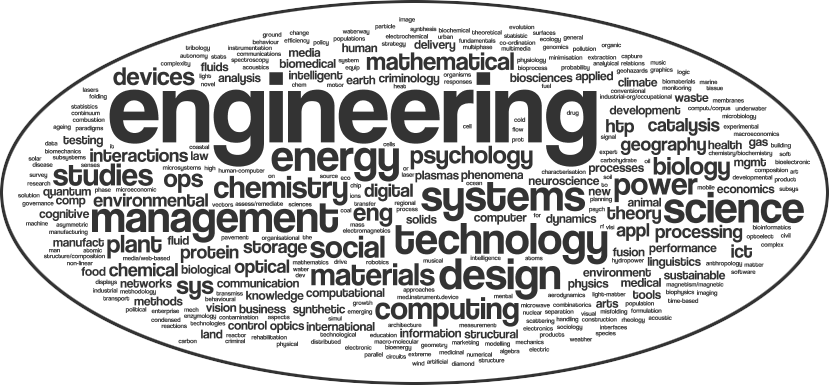
\includegraphics[width=\textwidth,height=\textheight,keepaspectratio]{word-clouds/frequency/all}
    \caption[Word cloud representation based on word frequency showcasing words that formulate topics in the \textit{Topic-grant} network]{Word cloud representation showcasing words that formulate topics in the \textit{Topic-grant} network constructed using the current (2010 to 2016) data set. Font size represents of word frequency within the the text corpus.}
    \label{fig:topic_a_current_freq_all}
\end{figure}

\vspace{3em}

\begin{figure}[htbp]
    \centering
    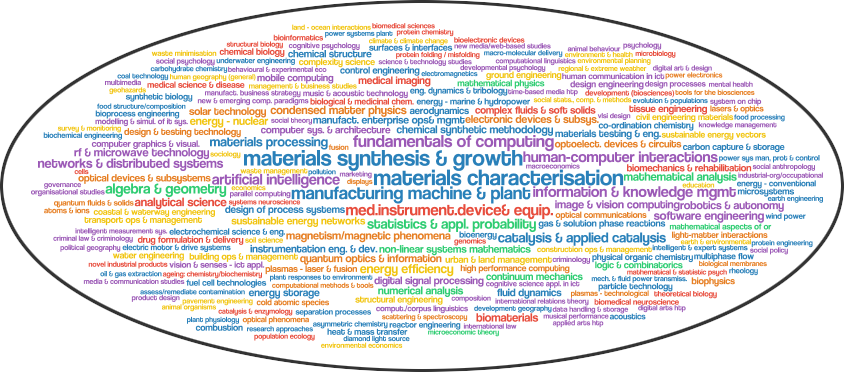
\includegraphics[width=\textwidth,height=\textheight,keepaspectratio]{word-clouds/number/all}
    \caption[Word cloud representation based on the number of grants containing the topics in the \textit{Topic-grant} network]{Word cloud representation showcasing the topics in the \textit{Topic-grant} network constructed using the current (2010 to 2016) data set. Font size represents the number of grants each topic appears in.}
    \label{fig:topic_a_current_number_all}
\end{figure}

\clearpage

\begin{figure}[htbp]
    \centering
    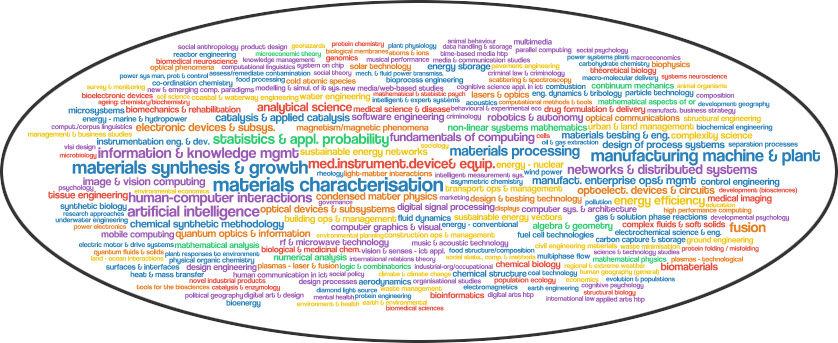
\includegraphics[width=\textwidth,height=\textheight,keepaspectratio]{word-clouds/value/all}
    \caption[Word cloud representation based on the value of grants containing the topics in the \textit{Topic-grant} network]{Word cloud representation showcasing the topics in the \textit{Topic-grant} network constructed using the current (2010 to 2016) data set. Font size represents the number of grants each topic appears in.}
    \label{fig:topic_a_current_value_all}
\end{figure}

\begin{spacing}{0.9}
\begin{longtable}[c]{r|>{\raggedleft\arraybackslash}m{6.5cm}|>{\raggedleft\arraybackslash}m{1.9cm}|r}
\caption[Topics and the number and value of grants that contain each topic in the \textit{Topic-grant} network constructed using the current (2010 to 2016) data set]{Topics and the number and value of grants that contain each topic sorted by the number of grants (largest to smallest) in the \textit{Topic-grant} network constructed using the current (2010 to 2016) data set}\\
\label{table:topic_a_current_topics_appendix}
\textbf{No.} & \textbf{Topic} & \textbf{Number of Grants} & \textbf{Value of Grants}\\
\hline
\endfirsthead
\caption[]{Continued from previous page.}\\
\textbf{No.} & \textbf{Topic} & \textbf{Number of Grants} & \textbf{Value of Grants}\\
\hline
\endhead
{1} & {materials synthesis \& growth} & {273} & {\pounds305,344,034.00}\\
{2} & {materials characterisation} & {270} & {\pounds350,845,612.00}\\
{3} & {manufacturing machine \& plant} & {196} & {\pounds273,265,770.00}\\
{4} & {fundamentals of computing} & {175} & {\pounds140,728,848.00}\\
{5} & {med.instrument.device\& equip.} & {155} & {\pounds192,497,214.00}\\
{6} & {human-computer interactions} & {147} & {\pounds193,369,943.00}\\
{7} & {artificial intelligence} & {146} & {\pounds231,826,208.00}\\
{8} & {information \& knowledge mgmt} & {141} & {\pounds211,234,642.00}\\
{9} & {algebra \& geometry} & {131} & {\pounds69,459,955.00}\\
{10} & {catalysis \& applied catalysis} & {124} & {\pounds116,914,672.00}\\
{11} & {statistics \& appl. probability} & {120} & {\pounds200,779,552.00}\\
{12} & {networks \& distributed systems} & {110} & {\pounds177,563,885.00}\\
{13} & {materials processing} & {108} & {\pounds203,775,655.00}\\
{14} & {energy efficiency} & {100} & {\pounds150,990,954.00}\\
{15} & {analytical science} & {90} & {\pounds145,977,721.00}\\
{16} & {software engineering} & {87} & {\pounds92,094,590.00}\\
{17} & {mathematical analysis} & {86} & {\pounds56,207,447.00}\\
{18} & {condensed matter physics} & {82} & {\pounds97,207,707.00}\\
{19} & {biomaterials} & {81} & {\pounds101,030,647.00}\\
{20} & {rf \& microwave technology} & {81} & {\pounds71,900,374.00}\\
{21} & {energy - nuclear} & {79} & {\pounds77,162,994.00}\\
{22} & {robotics \& autonomy} & {77} & {\pounds93,009,453.00}\\
{23} & {image \& vision computing} & {74} & {\pounds116,964,229.00}\\
{24} & {magnetism/magnetic phenomena} & {74} & {\pounds61,078,943.00}\\
{25} & {chemical synthetic methodology} & {72} & {\pounds101,788,856.00}\\
{26} & {electronic devices \& subsys.} & {72} & {\pounds123,197,049.00}\\
{27} & {numerical analysis} & {68} & {\pounds68,652,593.00}\\
{28} & {quantum optics \& information} & {68} & {\pounds99,752,497.00}\\
{29} & {energy storage} & {65} & {\pounds71,775,478.00}\\
{30} & {instrumentation eng. \& dev.} & {65} & {\pounds68,148,151.00}\\
{31} & {manufact. enterprise ops\& mgmt} & {65} & {\pounds119,063,980.00}\\
{32} & {non-linear systems mathematics} & {62} & {\pounds75,268,389.00}\\
{33} & {sustainable energy networks} & {62} & {\pounds91,222,489.00}\\
{34} & {digital signal processing} & {61} & {\pounds74,370,433.00}\\
{35} & {fluid dynamics} & {61} & {\pounds51,953,657.00}\\
{36} & {solar technology} & {61} & {\pounds40,262,413.00}\\
{37} & {medical imaging} & {60} & {\pounds73,682,425.00}\\
{38} & {continuum mechanics} & {57} & {\pounds56,547,841.00}\\
{39} & {materials testing \& eng.} & {57} & {\pounds94,707,839.00}\\
{40} & {complex fluids \& soft solids} & {54} & {\pounds51,883,688.00}\\
{41} & {optoelect. devices \& circuits} & {54} & {\pounds117,816,421.00}\\
{42} & {optical devices \& subsystems} & {53} & {\pounds99,280,018.00}\\
{43} & {chemical structure} & {52} & {\pounds57,198,101.00}\\
{44} & {computer sys. \& architecture} & {52} & {\pounds60,302,509.00}\\
{45} & {design of process systems} & {52} & {\pounds97,558,106.00}\\
{46} & {aerodynamics} & {50} & {\pounds51,110,961.00}\\
{47} & {biomechanics \& rehabilitation} & {47} & {\pounds62,830,082.00}\\
{48} & {mobile computing} & {46} & {\pounds67,914,107.00}\\
{49} & {tissue engineering} & {46} & {\pounds85,152,510.00}\\
{50} & {biophysics} & {45} & {\pounds44,234,268.00}\\
{51} & {control engineering} & {43} & {\pounds66,051,915.00}\\
{52} & {logic \& combinatorics} & {43} & {\pounds24,297,595.00}\\
{53} & {design \& testing technology} & {40} & {\pounds63,777,809.00}\\
{54} & {gas \& solution phase reactions} & {40} & {\pounds47,267,022.00}\\
{55} & {urban \& land management} & {39} & {\pounds73,439,680.00}\\
{56} & {chemical biology} & {38} & {\pounds64,182,393.00}\\
{57} & {co-ordination chemistry} & {38} & {\pounds25,587,639.00}\\
{58} & {complexity science} & {38} & {\pounds77,295,542.00}\\
{59} & {mathematical physics} & {38} & {\pounds27,981,443.00}\\
{60} & {plasmas - laser \& fusion} & {38} & {\pounds32,160,232.00}\\
{61} & {transport ops \& management} & {37} & {\pounds60,741,338.00}\\
{62} & {computer graphics \& visual.} & {36} & {\pounds68,214,771.00}\\
{63} & {design engineering} & {36} & {\pounds54,318,218.00}\\
{64} & {microsystems} & {36} & {\pounds57,061,520.00}\\
{65} & {surfaces \& interfaces} & {36} & {\pounds33,940,347.00}\\
{66} & {structural engineering} & {35} & {\pounds38,256,069.00}\\
{67} & {water engineering} & {35} & {\pounds64,215,111.00}\\
{68} & {carbon capture \& storage} & {34} & {\pounds36,659,546.00}\\
{69} & {drug formulation \& delivery} & {34} & {\pounds55,765,735.00}\\
{70} & {building ops \& management} & {33} & {\pounds67,993,377.00}\\
{71} & {combustion} & {33} & {\pounds27,342,322.00}\\
{72} & {ground engineering} & {33} & {\pounds32,605,304.00}\\
{73} & {civil engineering materials} & {31} & {\pounds19,613,822.00}\\
{74} & {coastal \& waterway engineering} & {31} & {\pounds22,329,706.00}\\
{75} & {electrochemical science \& eng.} & {31} & {\pounds30,783,229.00}\\
{76} & {sustainable energy vectors} & {31} & {\pounds63,410,664.00}\\
{77} & {eng. dynamics \& tribology} & {30} & {\pounds36,426,390.00}\\
{78} & {medical science \& disease} & {30} & {\pounds56,249,992.00}\\
{79} & {synthetic biology} & {30} & {\pounds52,068,052.00}\\
{80} & {bioenergy} & {29} & {\pounds31,787,943.00}\\
{81} & {biological \& medicinal chem.} & {29} & {\pounds45,503,257.00}\\
{82} & {vision \& senses - ict appl.} & {29} & {\pounds25,991,424.00}\\
{83} & {fuel cell technologies} & {28} & {\pounds41,944,010.00}\\
{84} & {energy - marine \& hydropower} & {27} & {\pounds34,863,003.00}\\
{85} & {heat \& mass transfer} & {27} & {\pounds37,435,379.00}\\
{86} & {high performance computing} & {27} & {\pounds8,615,102.00}\\
{87} & {physical organic chemistry} & {27} & {\pounds20,341,238.00}\\
{88} & {particle technology} & {26} & {\pounds32,455,830.00}\\
{89} & {light-matter interactions} & {25} & {\pounds35,116,928.00}\\
{90} & {multiphase flow} & {25} & {\pounds24,773,814.00}\\
{91} & {optical communications} & {25} & {\pounds60,200,016.00}\\
{92} & {lasers \& optics} & {24} & {\pounds59,840,920.00}\\
{93} & {mathematical aspects of or} & {24} & {\pounds36,307,556.00}\\
{94} & {acoustics} & {23} & {\pounds15,766,542.00}\\
{95} & {cold atomic species} & {23} & {\pounds30,906,872.00}\\
{96} & {human communication in ict} & {23} & {\pounds26,806,703.00}\\
{97} & {reactor engineering} & {21} & {\pounds20,306,317.00}\\
{98} & {energy - conventional} & {20} & {\pounds37,659,404.00}\\
{99} & {bioprocess engineering} & {19} & {\pounds29,798,746.00}\\
{100} & {music \& acoustic technology} & {19} & {\pounds28,310,628.00}\\
{101} & {biomedical neuroscience} & {18} & {\pounds29,394,374.00}\\
{102} & {separation processes} & {18} & {\pounds18,158,126.00}\\
{103} & {wind power} & {17} & {\pounds27,401,527.00}\\
{104} & {bioinformatics} & {16} & {\pounds52,029,825.00}\\
{105} & {comput./corpus linguistics} & {14} & {\pounds6,931,002.00}\\
{106} & {design processes} & {14} & {\pounds22,405,461.00}\\
{107} & {atoms \& ions} & {13} & {\pounds6,214,215.00}\\
{108} & {construction ops \& management} & {13} & {\pounds24,891,070.00}\\
{109} & {electric motor \& drive systems} & {13} & {\pounds11,263,500.00}\\
{110} & {modelling \& simul. of it sys.} & {13} & {\pounds21,688,225.00}\\
{111} & {optical phenomena} & {13} & {\pounds24,315,772.00}\\
{112} & {quantum fluids \& solids} & {12} & {\pounds12,041,645.00}\\
{113} & {asymmetric chemistry} & {11} & {\pounds13,640,958.00}\\
{114} & {parallel computing} & {11} & {\pounds12,635,358.00}\\
{115} & {rheology} & {11} & {\pounds4,582,687.00}\\
{116} & {manufact. business strategy} & {10} & {\pounds11,140,214.00}\\
{117} & {fusion} & {9} & {\pounds190,002,289.00}\\
{118} & {management \& business studies} & {8} & {\pounds17,784,633.00}\\
{119} & {multimedia} & {8} & {\pounds31,132,743.00}\\
{120} & {plasmas - technological} & {8} & {\pounds10,160,650.00}\\
{121} & {psychology} & {8} & {\pounds9,857,802.00}\\
{122} & {theoretical biology} & {8} & {\pounds32,975,270.00}\\
{123} & {cognitive psychology} & {7} & {\pounds3,369,386.00}\\
{124} & {cognitive science appl. in ict} & {7} & {\pounds7,657,173.00}\\
{125} & {new \& emerging comp. paradigms} & {7} & {\pounds17,376,463.00}\\
{126} & {biochemical engineering} & {6} & {\pounds18,986,493.00}\\
{127} & {social psychology} & {6} & {\pounds4,160,146.00}\\
{128} & {soil science} & {6} & {\pounds2,458,999.00}\\
{129} & {system on chip} & {6} & {\pounds12,898,174.00}\\
{130} & {underwater engineering} & {6} & {\pounds7,492,407.00}\\
{131} & {waste management} & {6} & {\pounds12,104,515.00}\\
{132} & {waste minimisation} & {6} & {\pounds8,717,814.00}\\
{133} & {bioelectronic devices} & {5} & {\pounds22,042,473.00}\\
{134} & {criminology} & {5} & {\pounds5,080,147.00}\\
{135} & {development (biosciences)} & {5} & {\pounds2,325,834.00}\\
{136} & {genomics} & {5} & {\pounds24,454,128.00}\\
{137} & {intelligent \& expert systems} & {5} & {\pounds9,297,777.00}\\
{138} & {organisational studies} & {5} & {\pounds5,952,437.00}\\
{139} & {power sys man, prot \& control} & {5} & {\pounds2,609,392.00}\\
{140} & {digital art \& design} & {4} & {\pounds18,465,875.00}\\
{141} & {food processing} & {4} & {\pounds7,452,606.00}\\
{142} & {new media/web-based studies} & {4} & {\pounds25,232,837.00}\\
{143} & {vlsi design} & {4} & {\pounds7,404,543.00}\\
{144} & {assess/remediate contamination} & {3} & {\pounds4,534,982.00}\\
{145} & {climate \& climate change} & {3} & {\pounds1,750,258.00}\\
{146} & {criminal law \& criminology} & {3} & {\pounds5,019,737.00}\\
{147} & {displays} & {3} & {\pounds11,749,150.00}\\
{148} & {economics} & {3} & {\pounds11,015,140.00}\\
{149} & {electromagnetics} & {3} & {\pounds6,188,182.00}\\
{150} & {food structure/composition} & {3} & {\pounds5,141,921.00}\\
{151} & {macro-molecular delivery} & {3} & {\pounds7,026,191.00}\\
{152} & {media \& communication studies} & {3} & {\pounds12,545,468.00}\\
{153} & {pavement engineering} & {3} & {\pounds10,890,078.00}\\
{154} & {population ecology} & {3} & {\pounds16,690,970.00}\\
{155} & {scattering \& spectroscopy} & {3} & {\pounds7,558,809.00}\\
{156} & {social policy} & {3} & {\pounds1,942,868.00}\\
{157} & {tools for the biosciences} & {3} & {\pounds4,221,581.00}\\
{158} & {catalysis \& enzymology} & {2} & {\pounds689,340.00}\\
{159} & {cells} & {2} & {\pounds6,116,997.00}\\
{160} & {digital arts htp} & {2} & {\pounds12,062,042.00}\\
{161} & {environment \& health} & {2} & {\pounds568,459.00}\\
{162} & {governance} & {2} & {\pounds1,097,691.00}\\
{163} & {knowledge management} & {2} & {\pounds1,056,671.00}\\
{164} & {marketing} & {2} & {\pounds1,015,702.00}\\
{165} & {mathematical \& statistic psych} & {2} & {\pounds1,117,398.00}\\
{166} & {microeconomic theory} & {2} & {\pounds842,950.00}\\
{167} & {oil \& gas extraction} & {2} & {\pounds2,642,452.00}\\
{168} & {plant physiology} & {2} & {\pounds1,198,745.00}\\
{169} & {political geography} & {2} & {\pounds7,455,498.00}\\
{170} & {power electronics} & {2} & {\pounds2,270,158.00}\\
{171} & {power systems plant} & {2} & {\pounds3,941,441.00}\\
{172} & {protein chemistry} & {2} & {\pounds389,453.00}\\
{173} & {regional \& extreme weather} & {2} & {\pounds2,750,487.00}\\
{174} & {social anthropology} & {2} & {\pounds6,771,898.00}\\
{175} & {structural biology} & {2} & {\pounds524,187.00}\\
{176} & {ageing: chemistry/biochemistry} & {1} & {\pounds475,926.00}\\
{177} & {animal behaviour} & {1} & {\pounds506,361.00}\\
{178} & {animal organisms} & {1} & {\pounds1,581,410.00}\\
{179} & {applied arts htp} & {1} & {\pounds6,358,107.00}\\
{180} & {behavioural \& experimental eco} & {1} & {\pounds1,975,496.00}\\
{181} & {biological membranes} & {1} & {\pounds2,215.00}\\
{182} & {biomedical sciences} & {1} & {\pounds188,407.00}\\
{183} & {carbohydrate chemistry} & {1} & {\pounds920,060.00}\\
{184} & {coal technology} & {1} & {\pounds6,550,555.00}\\
{185} & {composition} & {1} & {\pounds5,971,211.00}\\
{186} & {computational linguistics} & {1} & {\pounds340,421.00}\\
{187} & {computational methods \& tools} & {1} & {\pounds98,603.00}\\
{188} & {data handling \& storage} & {1} & {\pounds742,513.00}\\
{189} & {development geography} & {1} & {\pounds241,076.00}\\
{190} & {developmental psychology} & {1} & {\pounds559,077.00}\\
{191} & {diamond light source} & {1} & {\pounds1,436,518.00}\\
{192} & {earth \& environmental} & {1} & {\pounds1,581,410.00}\\
{193} & {earth engineering} & {1} & {\pounds1,000,951.00}\\
{194} & {education} & {1} & {\pounds3,444,605.00}\\
{195} & {environmental economics} & {1} & {\pounds2,926.00}\\
{196} & {environmental planning} & {1} & {\pounds3,567,862.00}\\
{197} & {evolution \& populations} & {1} & {\pounds1,190,209.00}\\
{198} & {geohazards} & {1} & {\pounds246,258.00}\\
{199} & {human geography (general)} & {1} & {\pounds3,567,862.00}\\
{200} & {industrial-org/occupational} & {1} & {\pounds3,793,546.00}\\
{201} & {intelligent measurement sys.} & {1} & {\pounds4,956,495.00}\\
{202} & {international law} & {1} & {\pounds1,975,496.00}\\
{203} & {international relations theory} & {1} & {\pounds3,489,111.00}\\
{204} & {land - ocean interactions} & {1} & {\pounds1,415,336.00}\\
{205} & {macroeconomics} & {1} & {\pounds4,000,602.00}\\
{206} & {mech. \& fluid power transmiss.} & {1} & {\pounds514,747.00}\\
{207} & {mental health} & {1} & {\pounds294,021.00}\\
{208} & {microbiology} & {1} & {\pounds404,819.00}\\
{209} & {musical performance} & {1} & {\pounds5,971,211.00}\\
{210} & {novel industrial products} & {1} & {\pounds7,174,439.00}\\
{211} & {plant responses to environment} & {1} & {\pounds1,190,209.00}\\
{212} & {pollution} & {1} & {\pounds6,531,178.00}\\
{213} & {product design} & {1} & {\pounds5,965,328.00}\\
{214} & {protein engineering} & {1} & {\pounds1,015,843.00}\\
{215} & {protein folding / misfolding} & {1} & {\pounds458,233.00}\\
{216} & {research approaches} & {1} & {\pounds691,643.00}\\
{217} & {science \& technology studies} & {1} & {\pounds2,667,741.00}\\
{218} & {social stats., comp. \& methods} & {1} & {\pounds3,444,605.00}\\
{219} & {social theory} & {1} & {\pounds775,542.00}\\
{220} & {sociology} & {1} & {\pounds3,567,862.00}\\
{221} & {survey \& monitoring} & {1} & {\pounds246,258.00}\\
{222} & {systems neuroscience} & {1} & {\pounds100,803.00}\\
{223} & {time-based media htp} & {1} & {\pounds6,358,107.00}
\end{longtable}
\end{spacing}

\begin{table}[!htbp]
\centering
\caption[Properties of the \textit{Topic-grant} network constructed using the current (2010 to 2016) data set]{Properties of the \textit{Topic-grant} network constructed using the current (2010 to 2016) data set. Three of the column names are abbreviated: \textbf{uw}, \textbf{wnn} and \textbf{wnv} stand for unweighted, weighted by normalized number of grants and weighted by normalized value of grants, respectively.}
\label{table:topic_a_current_stats_appendix}
\begin{tabular}{r|rrrrr}
\textbf{} & \textbf{uw} & \textbf{wnn} & \textbf{wnv}\\
\hline
\textbf{Nodes} & {223} & {223} & {223}\\
\textbf{Edges} & {2008} & {2008} & {2008}\\
\textbf{Type} & {Undirected} & {Undirected} & {Undirected}\\
\textbf{Weighted} & {No} & {Yes} & {Yes}\\
\textbf{Connected} & {Yes} & {Yes} & {Yes}\\
\textbf{Average Degree} & {18.009} & {18.009} & {18.009}\\
\textbf{Average Weighted Degree} & {-} & {19.543} & {22.35}\\
\textbf{Diameter} & {5} & {5} & {6}\\
\textbf{Radius} & {3} & {3} & {3}\\
\textbf{Density} & {0.081} & {0.081} & {0.081}\\
\textbf{Modularity} & {0.347} & {0.373} & {0.385}\\
\textbf{Communities} & {5} & {6} & {6}\\
%\textbf{Weak Components} & {1} & {1} & {1}\\
\textbf{Node Closeness} & {0.426} & {0.423} & {0.412}\\
\textbf{Node Betweenness} & {154.839} & {156.483} & {162.633}\\
\textbf{Edge Betweenness} & {29.523} & {29.706} & {30.389}\\
\textbf{Average Clustering Coefficient} & {0.597} & {0.597} & {0.597}\\
%\textbf{Eigenvector Centrality} & {0.252} & {0.204} & {0.183}\\
\textbf{Average Path Length} & {2.395} & {2.395} & {2.395}
\end{tabular}
\end{table}

\clearpage

\begin{table}[!htbp]
\centering
\caption[Number of communities and modularity score of the community structure identified within the \textit{Topic-grant} network constructed using the current (2010 to 2016) data set]{Number of communities identified (left value) and the modularity score of the community structure discovered (right value) as a result of applying several community detection algorithms to the \textit{Topic-grant} network constructed using the current (2010 to 2016) data set. Three of the column names are abbreviated: \textbf{uw}, \textbf{wnn} and \textbf{wnv} stand for unweighted, weighted by normalized number of grants and weighted by normalized value of grants, respectively.}
\label{table:topic_a_current_modularity_appendix}
\begin{tabular}{r|rr|rr|rr}
\textbf{} & \multicolumn{2}{c|}{\textbf{uw}} & \multicolumn{2}{c|}{\textbf{wnn}} & \multicolumn{2}{c}{\textbf{wnv}}\\
\hline
\textbf{Infomap}             & {3}   & {0.004} & {9}   & {0.332} & {11}  & {0.377}\\
\textbf{Spinglass}           & {6}   & {0.355} & {5}   & {0.375} & {5}   & {0.392}\\
\textbf{Louvain}             & {5}   & {0.347} & {6}   & {0.373} & {6}   & {0.385}\\
\textbf{Label Propagation}   & {1}   & {0.0}   & {1}   & {0.0}   & {1}   & {0.0}\\
\textbf{Leading Eigenvector} & {5}   & {0.312} & {5}   & {0.302} & {10}  & {0.311}\\
\textbf{Walktrap}            & {5}   & {0.279} & {19}  & {0.295} & {24}  & {0.328}\\
\textbf{Fast Greedy}         & {5}   & {0.314} & {4}   & {0.359} & {5}   & {0.369}\\
\textbf{Edge Betweenness}    & {164} & {0.038} & {166} & {0.042} & {105} & {0.15}
\end{tabular}
\end{table}

\begin{table}[!htbp]
\centering
\caption[Number of topics clustered within each community discovered in the \textit{Topic-grant} network constructed using the current (2010 to 2016) data set]{Number of topics clustered within each community discovered as a result of applying several community detection algorithms to the \textit{Topic-grant} network constructed using the current (2010 to 2016) data set. Six of the column names are abbreviated: \textbf{C1} stands for Community 1, \textbf{C2} for Community 2 and so on. Three of the row names are abbreviated: \textbf{uw}, \textbf{wnn} and \textbf{wnv} stand for unweighted, weighted by normalized number of grants and weighted by normalized value of grants, respectively.}
\label{table:topic_a_current_numbers_appendix}
\begin{tabular}{r|r|r|r|r|r|r|r}
\textbf{} & \textbf{} & \textbf{C1} & \textbf{C2} & \textbf{C3} & \textbf{C4} & \textbf{C5} & \textbf{C6}\\
\hline
\multirow{3}{*}{\textbf{uw}}
& \textbf{Spinglass}   & {35} & {60} & {25} & {53} & {36} & {14}\\
& \textbf{Louvain}     & {46} & {61} & {36} & {60} & {20} & {-}\\
& \textbf{Fast Greedy} & {95} & {57} & {60} & {8} & {3}   & {-}\\
\hline
\multirow{3}{*}{\textbf{wnn}}
& \textbf{Spinglass}   & {61} & {35} & {37} & {30} & {60} & {-}\\
& \textbf{Louvain}     & {29} & {61} & {63} & {10} & {34} & {26}\\
& \textbf{Fast Greedy} & {35} & {84} & {66} & {38} & {-}  & {-}\\
\hline
\multirow{3}{*}{\textbf{wnv}}
& \textbf{Spinglass}   & {63} & {17} & {51} & {63} & {29} & {-}\\
& \textbf{Louvain}     & {46} & {9}  & {29} & {61} & {43} & {35}\\
& \textbf{Fast Greedy} & {24} & {75} & {69} & {33} & {22} & {-}
\end{tabular}
\end{table}

\begin{table}[!htbp]
\centering
\caption[Number and value of grants within each community discovered in the \textit{Topic-grant} network constructed using the current (2010 to 2016) data set]{Number and value of grants within each community discovered as a result of applying several community detection algorithms to the \textit{Topic-grant} network constructed using the current (2010 to 2016) data set. The number of grants includes duplicate grants, as a grant can be part of more than one community. Subsequently, the value of grants also includes the duplicate grants. Six of the column names are abbreviated: \textbf{C1} stands for Community 1, \textbf{C2} for Community 2 and so on. Twelve of the row names are abbreviated: \textbf{uw}, \textbf{wnn} and \textbf{wnv} stand for unweighted, weighted by normalized number of grants and weighted by normalized value of grants, respectively. \textbf{SG}, \textbf{LV} and \textbf{FG} stand for the Spinglass, Louvain and Fast Greedy community detection algorithms.}
\label{table:topic_a_current_grants1_appendix}
\begin{tabular}{r|r|r|r|r|r|r|r|r}
\multicolumn{2}{c|}{} & \textbf{C1} & \textbf{C2} & \textbf{C3} & \textbf{C4} & \textbf{C5} & \textbf{C6} & \textbf{Total}\\
\hline
\multirow{6}{*}{\textbf{uw}}
& \multirow{2}{*}{\textbf{SG}}
& {376} & {727} & {483} & {1402} & {711} & {185} & {3884}\\
& {} & {\pounds468M} & {\pounds830M} & {\pounds769M} & {\pounds1.6B} & {\pounds769M} & {232M} & {\pounds4.7B}\\
\cline{2-9}
& \multirow{2}{*}{\textbf{LV}}
& {590} & {1351} & {685} & {727} & {583} & {-} & {3936}\\
& {} & {\pounds689M} & {\pounds1.7B} & {\pounds843M} & {\pounds830M} & {\pounds729M} & {-} & {\pounds4.8B}\\
\cline{2-9}
& \multirow{2}{*}{\textbf{FG}}
& {1810} & {1014} & {773} & {177} & {2} & {-} & {3776}\\
& {}& {\pounds2B} & {\pounds1.3B} & {\pounds855M} & {\pounds294M} & {1.2M} & {-} & {\pounds4.5B}\\
\hline
\multirow{6}{*}{\textbf{wnn}}
& \multirow{2}{*}{\textbf{SG}}
& {774} & {453} & {772} & {485} & {1376} & {-} & {3860}\\
& {} & {\pounds862M} & {\pounds542M} & {\pounds892M} & {\pounds766M} & {\pounds1.6B} & {-} & {\pounds4.7B}\\
\cline{2-9}
& \multirow{2}{*}{\textbf{LV}}
& {511} & {774} & {1338} & {317} & {480} & {484} & {3904}\\
& {} & {\pounds629M} & {\pounds862M} & {\pounds1.5B} & {\pounds332M} & {\pounds584M} & {\pounds766M} & {\pounds4.8B}\\
\cline{2-9}
& \multirow{2}{*}{\textbf{FG}}
& {718} & {1680} & {784} & {436} & {-} & {-} & {3618}\\
& {} & {\pounds801M} & {\pounds2.2B} & {\pounds894M} & {\pounds503M} & {-} & {-} & {\pounds4.4B}\\
\hline
\multirow{6}{*}{\textbf{wnv}}
& \multirow{2}{*}{\textbf{SG}}
& {1471} & {386} & {634} & {788} & {498} & {-} & {3777}\\
& {} & {\pounds1.8B} & {\pounds381M} & {\pounds716M} & {\pounds877M} & {\pounds607M} & {-} & {\pounds4.5B}\\
\cline{2-9}
& \multirow{2}{*}{\textbf{LV}}
& {1243} & {317} & {545} & {659} & {565} & {620} & {3949}\\
& {} & {\pounds1.4B} & {\pounds332M} & {\pounds814M} & {\pounds756M} & {\pounds662M} & {\pounds749M} & {4.8B}\\
\cline{2-9}
& \multirow{2}{*}{\textbf{FG}}
& {451} & {1732} & {887} & {253} & {402} & {-} & {3725}\\
& {} & {\pounds418M} & {\pounds2B} & {\pounds1B} & {\pounds295M} & {\pounds713M} & {-} & {\pounds4.5B}\\
\end{tabular}
\end{table}

\begin{table}[!htbp]
\centering
\caption[Total number and value of unique grants within communities, total number and value of unique grants within the network and total number and value of unique grants between communities discovered in the \textit{Topic-grant} network constructed using the current (2010 to 2016) data set]{Total number and value of unique grants within communities, total number and value of unique grants within the network and total number and value of unique grants between communities discovered as a result of applying several community detection algorithms to the \textit{Topic-grant} network constructed using the current (2010 to 2016) data set. Twelve of the row names are abbreviated: \textbf{uw}, \textbf{wnn} and \textbf{wnv} stand for unweighted, weighted by normalized number of grants and weighted by normalized value of grants, respectively. \textbf{SG}, \textbf{LV} and \textbf{FG} stand for the Spinglass, Louvain and Fast Greedy community detection algorithms.}
\label{table:topic_a_current_grants2_appendix}
\begin{tabular}{r|r|>{\raggedleft\arraybackslash}p{3.5cm}|>{\raggedleft\arraybackslash}p{3.2cm}|>{\raggedleft\arraybackslash}p{3.5cm}}
\multicolumn{2}{c|}{} & \textbf{Total number and value within communities (unique)} & \textbf{Total number and value within network (unique)} & \textbf{Total number and value between communities (unique)}\\
\hline
\multirow{6}{*}{\textbf{uw}}
& \multirow{2}{*}{\textbf{SG}}
& {3059} & {3103} & {44}\\
& {} & {\pounds3.51B} & {\pounds3.56B} & {\pounds42M}\\
\cline{2-5}
& \multirow{2}{*}{\textbf{LV}}
& {3071} & {3103} & {32}\\
& {} & {\pounds3.53B} & {\pounds3.56B} & {\pounds27M}\\
\cline{2-5}
& \multirow{2}{*}{\textbf{FG}}
& {3100} & {3103} & {3}\\
& {} & {\pounds3.55B} & {\pounds3.56B} & {\pounds2M}\\
\hline
\multirow{6}{*}{\textbf{wnn}}
& \multirow{2}{*}{\textbf{SG}}
& {3092} & {3103} & {11}\\
& {} & {\pounds3.55B} & {\pounds3.56B} & {\pounds4M}\\
\cline{2-5}
& \multirow{2}{*}{\textbf{LV}}
& {3072} & {3103} & {31}\\
& {} & {\pounds3.54B} & {\pounds3.56B} & {\pounds21M}\\
\cline{2-5}
& \multirow{2}{*}{\textbf{FG}}
& {3078} & {3103} & {25}\\
& {} & {\pounds3.53B} & {\pounds3.56B} & {\pounds26M}\\
\hline
\multirow{6}{*}{\textbf{wnv}}
& \multirow{2}{*}{\textbf{SG}}
& {3070} & {3103} & {33}\\
& {} & {\pounds3.53B} & {\pounds3.56B} & {\pounds22M}\\
\cline{2-5}
& \multirow{2}{*}{\textbf{LV}}
& {3077} & {3103} & {26}\\
& {} & {\pounds3.53B} & {\pounds3.56B} & {\pounds26M}\\
\cline{2-5}
& \multirow{2}{*}{\textbf{FG}}
& {3070} & {3103} & {33}\\
& {} & {\pounds3.53B} & {\pounds3.56B} & {\pounds23M}\\
\end{tabular}
\end{table}

\clearpage

\begin{figure}[htbp]
    \centering
    
\includegraphics[width=\textwidth,height=\textheight,keepaspectratio]{word-clouds/frequency/c1}
    \caption[Word cloud representation based on word frequency showcasing words that formulate topics clustered within Community 1]{Word cloud representation showcasing words that formulate the topics clustered within Community 1 in the \textit{Topic-grant} network by the optimal solution identified in the experiment. Font size represents the frequency of the word in the text corpus made out of all the words that formulate the topics clustered in Community 1.}
    \label{fig:topic_a_current_freq_c1_appendix}
\end{figure}

\vspace{10em}

\begin{figure}[htbp]
    \centering
    
\includegraphics[width=\textwidth,height=\textheight,keepaspectratio]{word-clouds/number/c1}
    \caption[Word cloud representation based on the number of grants containing topics clustered within Community 1]{Word cloud representation showcasing topics clustered within Community 1 in the \textit{Topic-grant} network by the optimal solution identified in the experiment. Font size represents the number of grants each topic appears in.}
    \label{fig:topic_a_current_number_c1_appendix}
\end{figure}

\clearpage

\begin{figure}[!htbp]
    \centering
    
\includegraphics[width=\textwidth,height=\textheight,keepaspectratio]{word-clouds/value/c1}
    \caption[Word cloud representation based on the value of grants containing topics clustered within Community 1]{Word cloud representation showcasing topics clustered within Community 1 in the \textit{Topic-grant} network by the optimal solution identified in the experiment. Font size represents the value of grants each topic appears in.}
    \label{fig:topic_a_current_value_c1_appendix}
\end{figure}

\vspace{8em}

\begin{figure}[htbp]
    \centering
    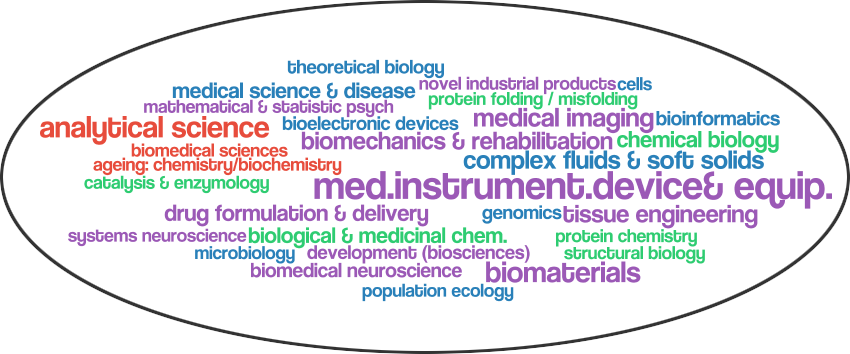
\includegraphics[width=\textwidth,height=\textheight,keepaspectratio]{word-clouds/number/sc1}
    \caption[Word cloud representation based on the number of grants containing topics in sub-communities within Community 1]{Word cloud representation showcasing topics in sub-communities within Community 1 in the \textit{Topic-grant} network by the optimal solution identified in the experiment. Font size represents the number of grants each topics appears in, while text colour represents the sub-communities identified within Community 1.}
    \label{fig:topic_a_current_number_sc1}
\end{figure}

\clearpage

\begin{figure}[htbp]
    \centering
    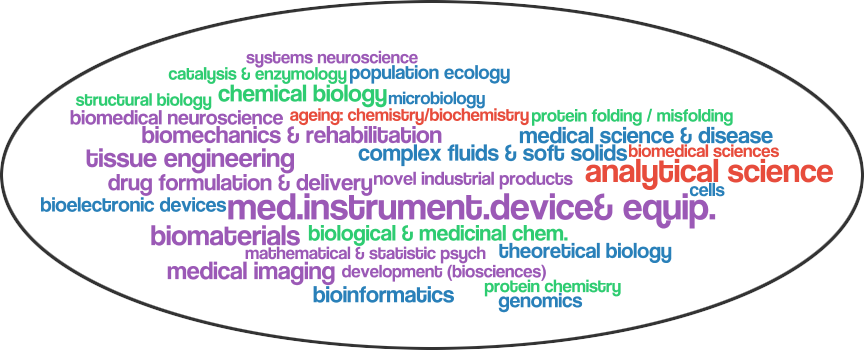
\includegraphics[width=\textwidth,height=\textheight,keepaspectratio]{word-clouds/value/sc1}
    \caption[Word cloud representation based on the value of grants containing topics in sub-communities within Community 1]{Word cloud representation showcasing topics in sub-communities within Community 1 in the \textit{Topic-grant} network by the optimal solution identified in the experiment. Font size represents the value of grants each topic appears in, while text colour represents the sub-communities identified within Community 1.}
    \label{fig:topic_a_current_value_sc1}
\end{figure}

\begin{spacing}{0.9}
\begin{longtable}[r]{r|r|p{11.5cm}}
\caption[Topics clustered within each sub-community of Community 1 discovered by the optimal solution identified in the experiment on the \textit{Topic-grant} network constructed using the current (2010 to 2016) data set]{Topics clustered within each sub-community of Community 1 discovered by the optimal solution identified in the experiment on the \textit{Topic-grant} network constructed using the current (2010 to 2016) data set. \textbf{C1} stands for Community 1. Rows representing sub-communities are named using second-level labels (1.1, 1.2 and so on).}\\
\label{table:topic_a_current_c1_appendix}
{} & {}\\
\hline
\endfirsthead
\caption[]{Continued from previous page.}\\
\endhead
\textbf{C1}
& \textbf{1.1} & {ageing: chemistry/biochemistry, analytical science, biomedical sciences}\\
& \textbf{1.2} & {biomaterials, med.instrument.device\& equip., biomechanics \& rehabilitation, medical imaging, biomedical neuroscience, novel industrial products, development (biosciences), systems neuroscience, drug formulation \& delivery, tissue engineering, mathematical \& statistic psych}\\
& \textbf{1.3} & {drug formulation \& delivery, tissue engineering, mathematical \& statistic psych, bioelectronic devices, medical science \& disease, bioinformatics, microbiology, cells, population ecology, complex fluids \& soft solids, theoretical biology, genomics}\\
& \textbf{1.4} & {biological \& medicinal chem., protein chemistry, catalysis \& enzymology, protein folding / misfolding, chemical biology, structural biology}
\end{longtable}
\end{spacing}

\clearpage

\begin{figure}[htbp]
    \centering
    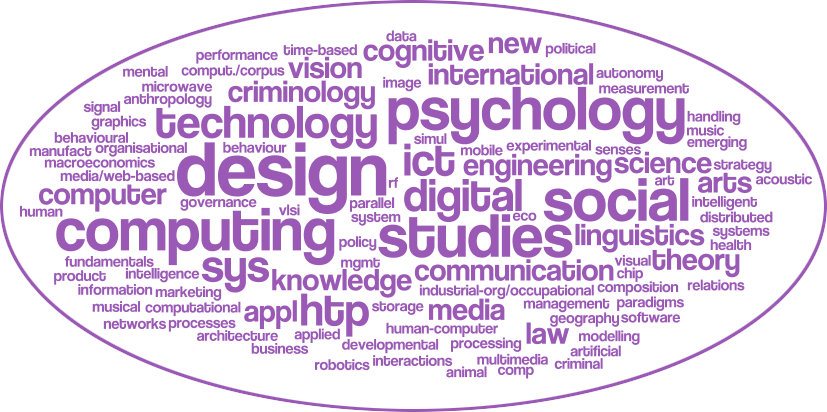
\includegraphics[width=\textwidth,height=\textheight,keepaspectratio]{word-clouds/frequency/c2}
    \caption[Word cloud representation based on word frequency showcasing words that formulate topics clustered within Community 2]{Word cloud representation showcasing words that formulate the topics clustered within Community 2 in the \textit{Topic-grant} network by the optimal solution identified in the experiment. Font size represents the frequency of the word in the text corpus made out of all the words that formulate the topics clustered in Community 2.}
    \label{fig:topic_a_current_freq_c2}
\end{figure}

\vspace{6em}

\begin{figure}[htbp]
    \centering
    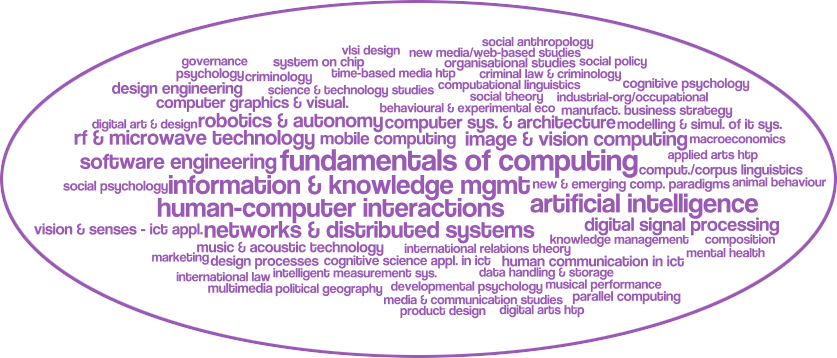
\includegraphics[width=\textwidth,height=\textheight,keepaspectratio]{word-clouds/number/c2}
    \caption[Word cloud representation based on the number of grants containing topics clustered within Community 2]{Word cloud representation showcasing topics clustered within Community 2 in the \textit{Topic-grant} network by the optimal solution identified in the experiment. Font size represents the number of grants each topic appears in.}
    \label{fig:topic_a_current_number_c2}
\end{figure}

\clearpage

\begin{figure}[htbp]
    \centering
    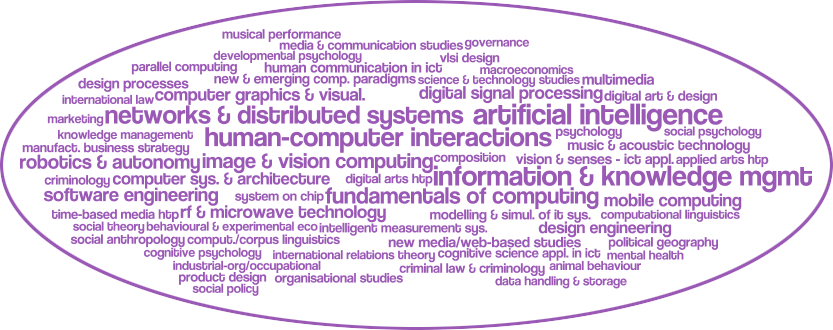
\includegraphics[width=\textwidth,height=\textheight,keepaspectratio]{word-clouds/value/c2}
    \caption[Word cloud representation based on the value of grants containing topics clustered within Community 2]{Word cloud representation showcasing topics clustered within Community 2 in the \textit{Topic-grant} network by the optimal solution identified in the experiment. Font size represents the number of grants each topic appears in.}
    \label{fig:topic_a_current_value_c2}
\end{figure}

\vspace{8em}

\begin{figure}[htbp]
    \centering
    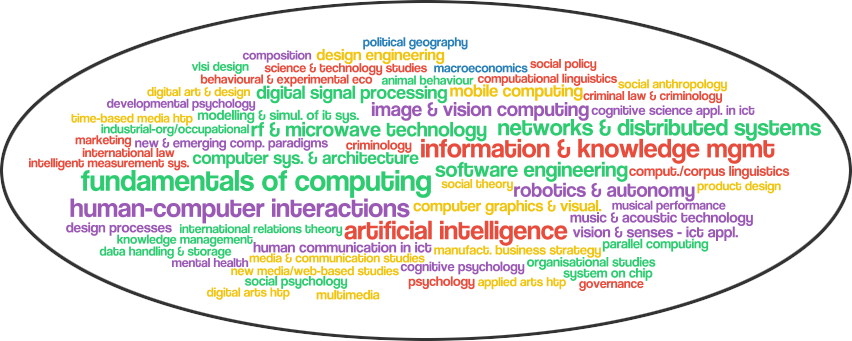
\includegraphics[width=\textwidth,height=\textheight,keepaspectratio]{word-clouds/number/sc2}
    \caption[Word cloud representation based on the number of grants containing topics in sub-communities within Community 2]{Word cloud representation showcasing topics in sub-communities within Community 2 in the \textit{Topic-grant} network by the optimal solution identified in the experiment. Font size represents the number of grants each topic appears in, while text colour represents the sub-communities identified within Community 2.}
    \label{fig:topic_a_current_number_sc2}
\end{figure}

\clearpage

\begin{figure}[htbp]
    \centering
    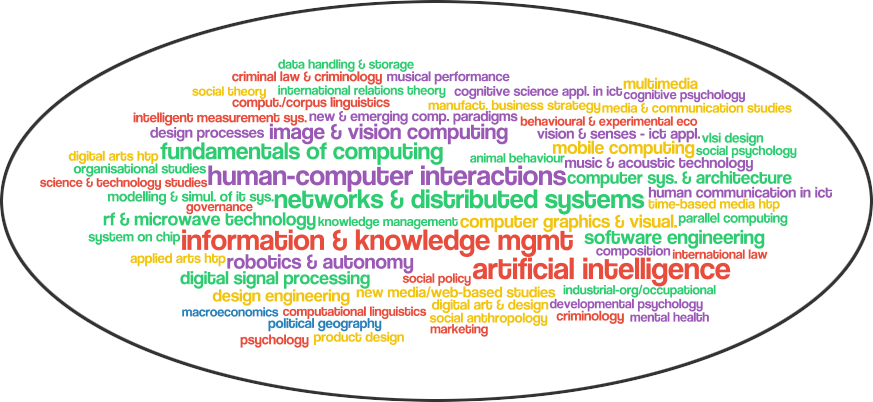
\includegraphics[width=\textwidth,height=\textheight,keepaspectratio]{word-clouds/value/sc2}
    \caption[Word cloud representation based on the value of grants containing topics in sub-communities within Community 2]{Word cloud representation showcasing topics in sub-communities within Community 2 in the \textit{Topic-grant} network by the optimal solution identified in the experiment. Font size represents the value of grants containing a specific topic, while text colour represents the sub-communities identified within Community 2.}
    \label{fig:topic_a_current_value_sc2}
\end{figure}

\begin{spacing}{0.9}
\begin{longtable}[r]{r|r|p{11.5cm}}
\caption[Topics clustered within each sub-community of Community 2 discovered by the optimal solution identified in the experiment on the \textit{Topic-grant} network constructed using the current (2010 to 2016) data set]{Topics clustered within each sub-community of Community 2 discovered by the optimal solution identified in the experiment on the \textit{Topic-grant} network constructed using the current (2010 to 2016) data set. \textbf{C2} for Community 2. Rows representing sub-communities are named using second-level labels (2.1, 2.2 and so on).}\\
\label{table:topic_a_current_c2_appendix}
{} & {}\\
\hline
\endfirsthead
\caption[]{Continued from previous page.}\\
\hline
\endhead
\textbf{C2}
& \textbf{2.1} & {artificial intelligence, information \& knowledge mgmt, behavioural \& experimental eco, intelligent measurement sys., comput./corpus linguistics, international law, computational linguistics, marketing, criminal law \& criminology, psychology, criminology, science \& technology studies, governance, social policy}\\
& \textbf{2.2} & {cognitive psychology, image \& vision computing, cognitive science appl. in ict, mental health, composition, music \& acoustic technology, design processes, musical performance, developmental psychology, new \& emerging comp. paradigms, human communication in ict, robotics \& autonomy, human-computer interactions, vision \& senses - ict appl.}\\
& \textbf{2.3} & {macroeconomics, political geography}\\
& \textbf{2.4} & {animal behaviour, networks \& distributed systems, computer sys. \& architecture, organisational studies, data handling \& storage, parallel computing, digital signal processing, rf \& microwave technology, fundamentals of computing, social psychology, industrial-org/occupational, software engineering, international relations theory, system on chip, knowledge management, vlsi design, modelling \& simul. of it sys.}\\
& \textbf{2.5} & {applied arts htp, mobile computing, computer graphics \& visual., multimedia, design engineering, new media/web-based studies, digital art \& design, product design, digital arts htp, social anthropology, manufact. business strategy, social theory, media \& communication studies, time-based media htp}
\end{longtable}
\end{spacing}

\clearpage

\begin{figure}[htbp]
    \centering
    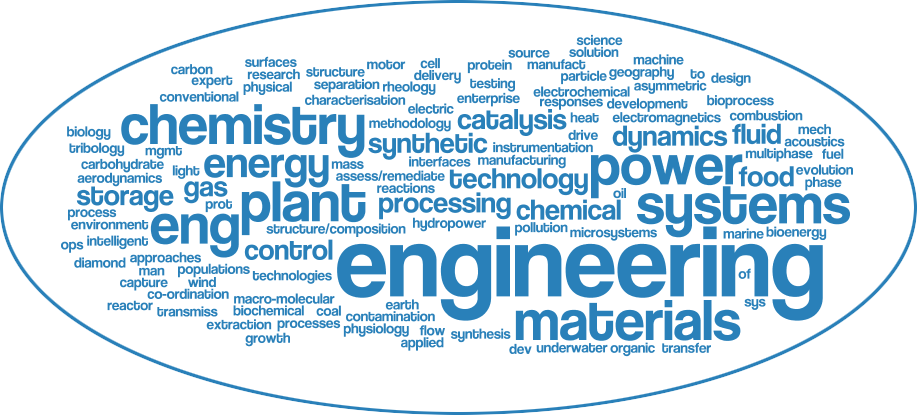
\includegraphics[width=\textwidth,height=\textheight,keepaspectratio]{word-clouds/frequency/c3}
    \caption[Word cloud representation based on word frequency showcasing words that formulate topics clustered within Community 3]{Word cloud representation showcasing words that formulate topics clustered within Community 1 in the \textit{Topic-grant} network by the optimal solution identified in the experiment. Font size represents the frequency of the word in the text corpus made out of all the words that formulate the topics clustered in Community 3.}
    \label{fig:topic_a_current_freq_c3}
\end{figure}

\vspace{6em}

\begin{figure}[htbp]
    \centering
    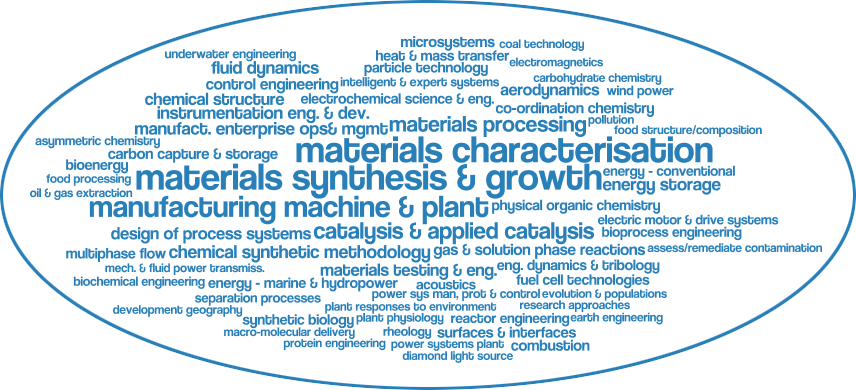
\includegraphics[width=\textwidth,height=\textheight,keepaspectratio]{word-clouds/number/c3}
    \caption[Word cloud representation based on the number of grants containing topics clustered within Community 3]{Word cloud representation showcasing topics clustered within Community 3 in the \textit{Topic-grant} network by the optimal solution identified in the experiment. Font size represents the number of grants each topic appears in.}
    \label{fig:topic_a_current_number_c3}
\end{figure}

\clearpage

\begin{figure}[htbp]
    \centering
    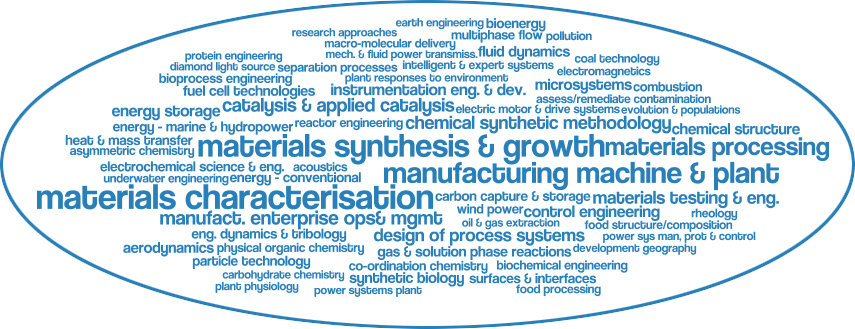
\includegraphics[width=\textwidth,height=\textheight,keepaspectratio]{word-clouds/value/c3}
    \caption[Word cloud representation based on the value of grants containing topics clustered within Community 3]{Word cloud representation showcasing topics clustered within Community 3 in the \textit{Topic-grant} network by the optimal solution identified in the experiment. Font size represents the number of grants each topic appears in.}
    \label{fig:topic_a_current_value_c3}
\end{figure}

\vspace{8em}

\begin{figure}[htbp]
    \centering
    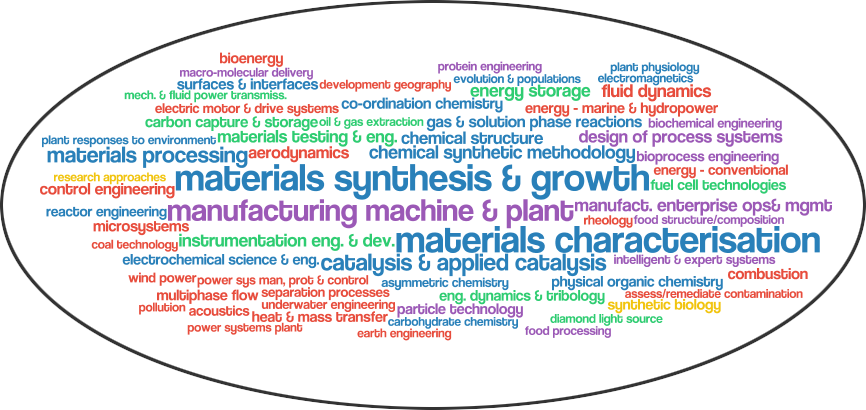
\includegraphics[width=\textwidth,height=\textheight,keepaspectratio]{word-clouds/number/sc3}
    \caption[Word cloud representation based on the number of grants containing topics in sub-communities within Community 3]{Word cloud representation showcasing topics in sub-communities within Community 3 in the \textit{Topic-grant} network by the optimal solution identified in the experiment. Font size represents the number of grants each topic appears in, while text colour represents the sub-communities identified within Community 3.}
    \label{fig:topic_a_current_number_sc3}
\end{figure}

\clearpage

\begin{figure}[htbp]
    \centering
    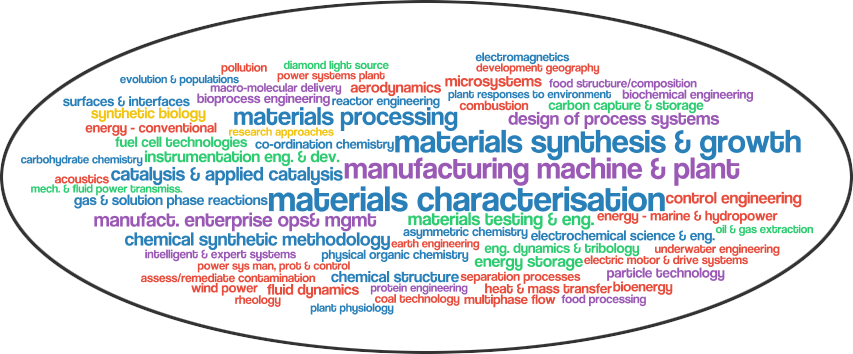
\includegraphics[width=\textwidth,height=\textheight,keepaspectratio]{word-clouds/value/sc3}
    \caption[Word cloud representation based on the value of grants containing topics in sub-communities within Community 3]{Word cloud representation showcasing topics in sub-communities within Community 3 in the \textit{Topic-grant} network by the optimal solution identified in the experiment. Font size represents the value of grants containing a specific topic, while text colour represents the sub-communities identified within Community 3.}
    \label{fig:topic_a_current_value_sc3}
\end{figure}

\begin{spacing}{0.9}
\begin{longtable}[r]{r|r|p{11.5cm}}
\caption[Topics clustered within each sub-community of Community 3 discovered by the optimal solution identified in the experiment on the \textit{Topic-grant} network constructed using the current (2010 to 2016) data set]{Topics clustered within each sub-community of Community 3 discovered by the optimal solution identified in the experiment on the \textit{Topic-grant} network constructed using the current (2010 to 2016) data set. \textbf{C3} stands for Community 3. Rows representing sub-communities are named using second-level labels (3.1, 3.2 and so on).}\\
\label{table:topic_a_current_c3_appendix}
{} & {}\\
\hline
\endfirsthead
\caption[]{Continued from previous page.}\\
\hline
\endhead
\textbf{C3}
& \textbf{3.1} & {acoustics, fluid dynamics, aerodynamics, heat \& mass transfer, assess/remediate contamination, microsystems, bioenergy, multiphase flow, coal technology, pollution, combustion, power sys man, prot \& control, control engineering, power systems plant, development geography, rheology, earth engineering, separation processes, electric motor \& drive systems, underwater engineering, energy - conventional, wind power, energy - marine \& hydropower}\\
& \textbf{3.2} & {biochemical engineering, macro-molecular delivery, bioprocess engineering, manufact. enterprise ops\& mgmt, design of process systems, manufacturing machine \& plant, food processing, particle technology, food structure/composition, protein engineering, intelligent \& expert systems}\\
& \textbf{3.3} & {asymmetric chemistry, gas \& solution phase reactions, carbohydrate chemistry, materials characterisation, catalysis \& applied catalysis, materials processing, chemical structure, materials synthesis \& growth, chemical synthetic methodology, physical organic chemistry, co-ordination chemistry, plant physiology, electrochemical science \& eng., plant responses to environment, electromagnetics, reactor engineering, evolution \& populations, surfaces \& interfaces}\\
& \textbf{3.4} & {carbon capture \& storage, instrumentation eng. \& dev., diamond light source, materials testing \& eng., energy storage, mech. \& fluid power transmiss., eng. dynamics \& tribology, oil \& gas extraction, fuel cell technologies}\\
& \textbf{3.5} & {research approaches, synthetic biology}\\
\end{longtable}
\end{spacing}

\clearpage

\begin{figure}[htbp]
    \centering
    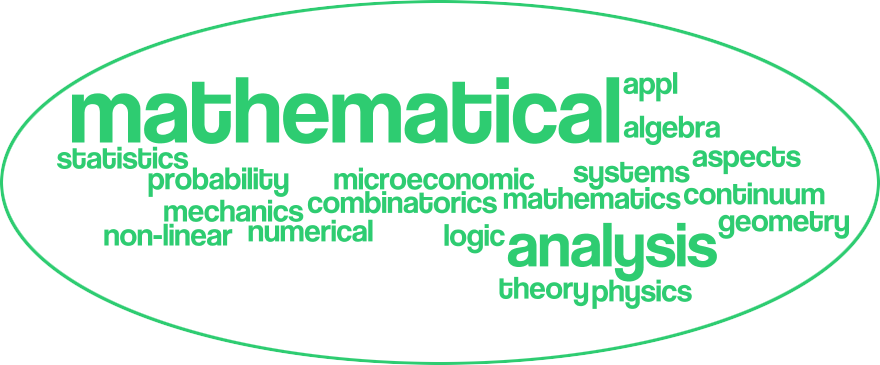
\includegraphics[width=\textwidth,height=\textheight,keepaspectratio]{word-clouds/frequency/c4}
    \caption[Word cloud representation based on word frequency showcasing words that formulate topics clustered within Community 4]{Word cloud representation showcasing words that formulate topics clustered within Community 4 in the \textit{Topic-grant} network by the optimal solution identified in the experiment. Font size represents the frequency of the word in the text corpus made out of all the words that formulate the topics clustered in Community 4.}
    \label{fig:topic_a_current_freq_c4}
\end{figure}

\vspace{10em}

\begin{figure}[htbp]
    \centering
    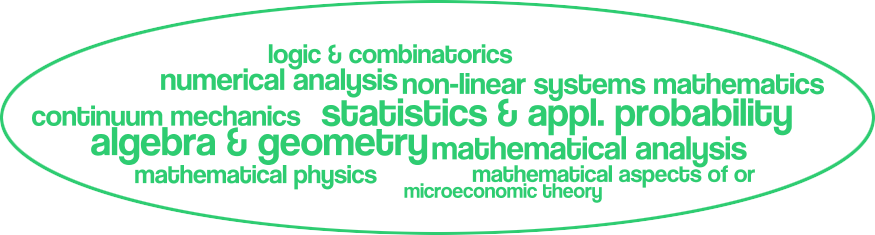
\includegraphics[width=\textwidth,height=\textheight,keepaspectratio]{word-clouds/number/c4}
    \caption[Word cloud representation based on the number of grants containing topics clustered within Community 4]{Word cloud representation showcasing topics clustered within Community 4 in the \textit{Topic-grant} network by the optimal solution identified in the experiment. Font size represents the number of grants each topic appears in.}
    \label{fig:topic_a_current_number_c4}
\end{figure}

\clearpage

\begin{figure}[htbp]
    \centering
    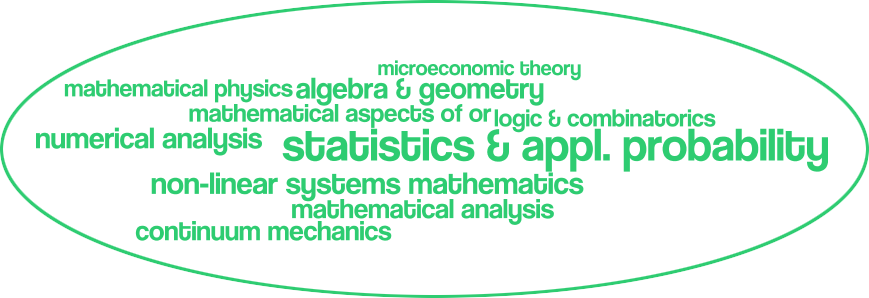
\includegraphics[width=\textwidth,height=\textheight,keepaspectratio]{word-clouds/value/c4}
    \caption[Word cloud representation based on the value of grants containing topics clustered within Community 4]{Word cloud representation showcasing topics clustered within Community 4 in the \textit{Topic-grant} network by the optimal solution identified in the experiment. Font size represents the number of grants each topic appears in.}
    \label{fig:topic_a_current_value_c4}
\end{figure}

\vspace{10em}

\begin{figure}[htbp]
    \centering
    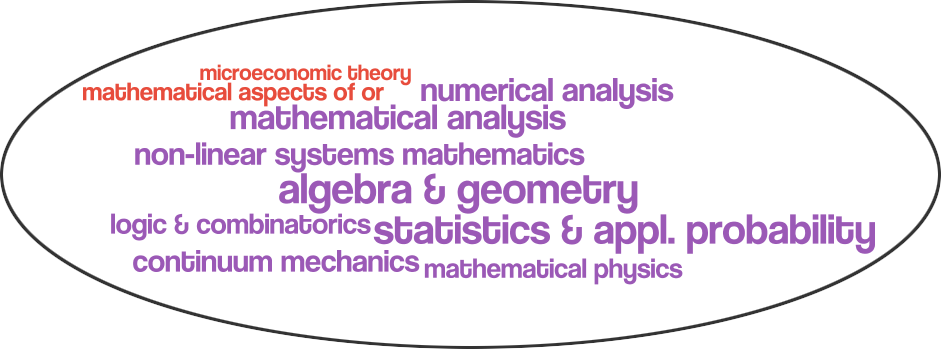
\includegraphics[width=\textwidth,height=\textheight,keepaspectratio]{word-clouds/number/sc4}
    \caption[Word cloud representation based on the number of grants containing topics in sub-communities within Community 4]{Word cloud representation showcasing topics in sub-communities within Community 4 in the \textit{Topic-grant} network by the optimal solution identified in the experiment. Font size represents the number of grants each topic appears in, while text colour represents the sub-communities identified within Community 4.}
    \label{fig:topic_a_current_number_sc4}
\end{figure}

\clearpage

\begin{figure}[htbp]
    \centering
    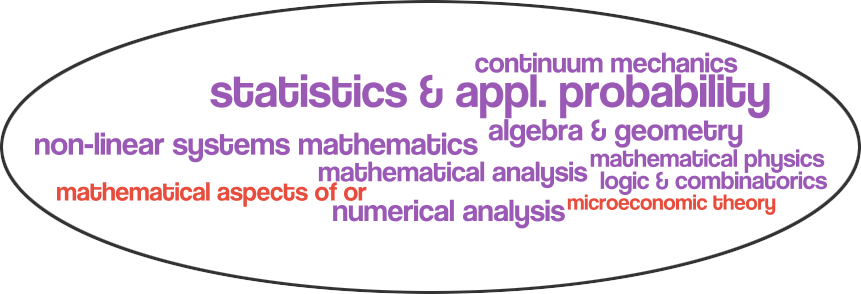
\includegraphics[width=\textwidth,height=\textheight,keepaspectratio]{word-clouds/value/sc4}
    \caption[Word cloud representation based on the value of grants containing topics in sub-communities within Community 4]{Word cloud representation showcasing topics in sub-communities within Community 4 in the \textit{Topic-grant} network by the optimal solution identified in the experiment. Font size represents the value of grants containing a specific topic, while text colour represents the sub-communities identified within Community 4.}
    \label{fig:topic_a_current_value_sc4}
\end{figure}

\begin{spacing}{0.9}
\begin{longtable}[r]{r|r|p{11.5cm}}
\caption[Topics clustered within each sub-community of Community 4 discovered by the optimal solution identified in the experiment on the \textit{Topic-grant} network constructed using the current (2010 to 2016) data set]{Topics clustered within each sub-community of Community 4 discovered by the optimal solution identified in the experiment on the \textit{Topic-grant} network constructed using the current (2010 to 2016) data set. \textbf{C4} stands for Community 4. Rows representing sub-communities are named using second-level labels (4.1, 4.2 and so on).}\\
\label{table:topic_a_current_c4_appendix}
{} & {}\\
\hline
\endfirsthead
\caption[]{Continued from previous page.}\\
\hline
\endhead
\textbf{C4}
& \textbf{4.1} & {mathematical aspects of or, microeconomic theory}\\
& \textbf{4.2} & {algebra \& geometry, mathematical physics, continuum mechanics, non-linear systems mathematics, logic \& combinatorics, numerical analysis, mathematical analysis, statistics \& appl. probability}\\
\end{longtable}
\end{spacing}

\clearpage

\begin{figure}[htbp]
    \centering
    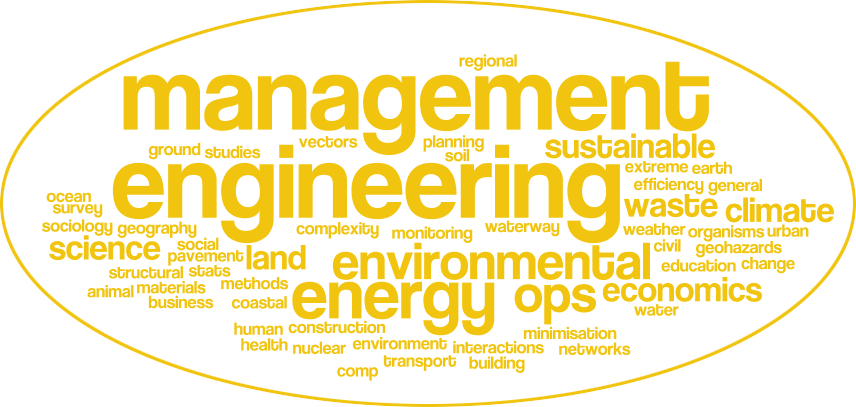
\includegraphics[width=\textwidth,height=\textheight,keepaspectratio]{word-clouds/frequency/c5}
    \caption[Word cloud representation based on word frequency showcasing words that formulate topics clustered within Community 5]{Word cloud representation showcasing words that formulate topics clustered within Community 5 in the \textit{Topic-grant} network by the optimal solution identified in the experiment. Font size represents the frequency of the word in the text corpus made out of all the words that formulate the topics clustered in Community 5.}
    \label{fig:topic_a_current_freq_c5}
\end{figure}

\vspace{6em}

\begin{figure}[htbp]
    \centering
    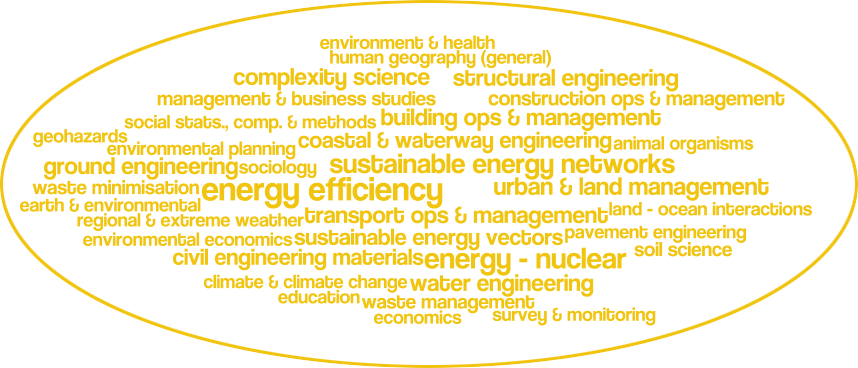
\includegraphics[width=\textwidth,height=\textheight,keepaspectratio]{word-clouds/number/c5}
    \caption[Word cloud representation based on the number of grants containing topics clustered within Community 5]{Word cloud representation showcasing topics clustered within Community 5 in the \textit{Topic-grant} network by the optimal solution identified in the experiment. Font size represents the number of grants each topic appears in.}
    \label{fig:topic_a_current_number_c5}
\end{figure}

\clearpage

\begin{figure}[htbp]
    \centering
    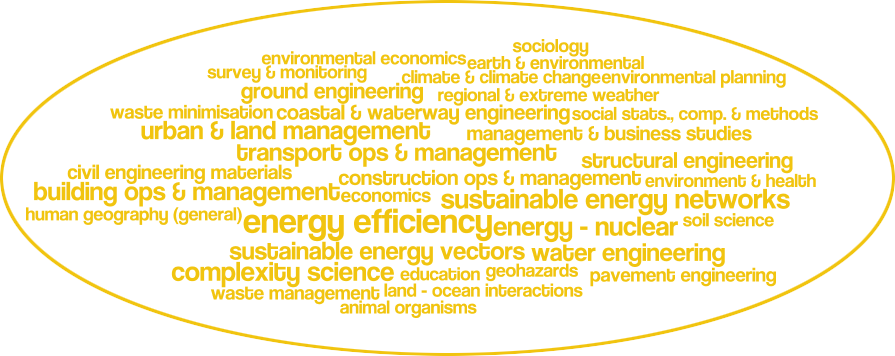
\includegraphics[width=\textwidth,height=\textheight,keepaspectratio]{word-clouds/value/c5}
    \caption[Word cloud representation based on the value of grants containing topics clustered within Community 5]{Word cloud representation showcasing topics clustered within Community 5 in the \textit{Topic-grant} network by the optimal solution identified in the experiment. Font size represents the number of grants each topic appears in.}
    \label{fig:topic_a_current_value_c5}
\end{figure}

\vspace{7em}

\begin{figure}[htbp]
    \centering
    \includegraphics[width=\textwidth,height=\textheight,keepaspectratio]{word-clouds/number/sc5}
    \caption[Word cloud representation based on the number of grants containing topics in sub-communities within Community 5]{Word cloud representation showcasing topics in sub-communities within Community 5 in the \textit{Topic-grant} network by the optimal solution identified in the experiment. Font size represents the number of grants each topic appears in, while text colour represents the sub-communities identified within Community 5.}
    \label{fig:topic_a_current_number_sc5}
\end{figure}

\clearpage

\begin{figure}[htbp]
    \centering
    \includegraphics[width=\textwidth,height=\textheight,keepaspectratio]{word-clouds/value/sc5}
    \caption[Word cloud representation based on the value of grants containing topics in sub-communities within Community 5]{Word cloud representation showcasing topics in sub-communities within Community 5 in the \textit{Topic-grant} network by the optimal solution identified in the experiment. Font size represents the value of grants containing a specific topic, while text colour represents the sub-communities identified within Community 5.}
    \label{fig:topic_a_current_value_sc5}
\end{figure}

\begin{spacing}{0.9}
\begin{longtable}[r]{r|r|p{11.5cm}}
\caption[Topics clustered within each sub-community of Community 5 discovered by the optimal solution identified in the experiment on the \textit{Topic-grant} network constructed using the current (2010 to 2016) data set]{Topics clustered within each sub-community of Community 5 discovered by the optimal solution identified in the experiment on the \textit{Topic-grant} network constructed using the current (2010 to 2016) data set. \textbf{C5} stands for Community 5. Rows representing sub-communities are named using second-level labels (5.1, 5.2 and so on).}\\
\label{table:topic_a_current_c5_appendix}
{} & {}\\
\hline
\endfirsthead
\caption[]{Continued from previous page.}\\
\hline
\endhead
\textbf{C5}
& \textbf{5.1} & {complexity science, management \& business studies, economics, social stats., comp. \& methods, education, sociology, environmental planning, sustainable energy networks, human geography (general), urban \& land management}\\
& \textbf{5.2} & {animal organisms, energy - nuclear, climate \& climate change, land - ocean interactions, coastal \& waterway engineering, regional \& extreme weather, earth \& environmental}\\
& \textbf{5.3} & {building ops \& management, pavement engineering, civil engineering materials, structural engineering, construction ops \& management, sustainable energy vectors, energy efficiency, waste management, environment \& health, waste minimisation, environmental economics, water engineering}\\
& \textbf{5.4} & {geohazards, survey \& monitoring, ground engineering, transport ops \& management, soil science}
\end{longtable}
\end{spacing}

\clearpage

\begin{figure}[htbp]
    \centering
    \includegraphics[width=\textwidth,height=\textheight,keepaspectratio]{word-clouds/frequency/c6}
    \caption[Word cloud representation based on word frequency showcasing words that formulate the topics clustered within Community 6]{Word cloud representation showcasing words that formulate topics clustered within Community 6 by the optimal solution identified in the experiment on the \textit{Topic-grant} network constructed using the current (2010 to 2016) data set. Font size represents the frequency of the word in the text corpus made out of all the words that formulate the topics clustered in Community 6.}
    \label{fig:topic_a_current_freq_c6}
\end{figure}

\vspace{7em}

\begin{figure}[htbp]
    \centering
    \includegraphics[width=\textwidth,height=\textheight,keepaspectratio]{word-clouds/number/c6}
    \caption[Word cloud representation based on the number of grants containing topics clustered within Community 6]{Word cloud representation showcasing topics clustered within Community 6 by the optimal solution identified in the experiment on the \textit{Topic-grant} network constructed using the current (2010 to 2016) data set. Font size represents the number of grants each topic appears in.}
    \label{fig:topic_a_current_number_c6}
\end{figure}

\clearpage

\begin{figure}[htbp]
    \centering
    \includegraphics[width=\textwidth,height=\textheight,keepaspectratio]{word-clouds/value/c6}
    \caption[Word cloud representation based on the value of grants containing topics clustered within Community 6]{Word cloud representation showcasing topics clustered within Community 6 by the optimal solution identified in the experiment on the \textit{Topic-grant} network constructed using the current (2010 to 2016) data set. Font size represents the number of grants each topic appears in.}
    \label{fig:topic_a_current_value_c6}
\end{figure}

\vspace{8em}

\begin{figure}[htbp]
    \centering
    \includegraphics[width=\textwidth,height=\textheight,keepaspectratio]{word-clouds/number/sc6}
    \caption[Word cloud representation based on the number of grants containing topics in sub-communities within Community 6]{Word cloud representation showcasing topics in sub-communities within Community 6 in the \textit{Topic-grant} network by the optimal solution identified in the experiment. Font size represents the number of grants each topic appears in, while text colour represents the sub-communities identified within Community 6.}
    \label{fig:topic_a_current_number_sc6}
\end{figure}

\clearpage

\begin{figure}[htbp]
    \centering
    \includegraphics[width=\textwidth,height=\textheight,keepaspectratio]{word-clouds/value/sc6}
    \caption[Word cloud representation based on the value of grants containing topics in sub-communities within Community 6]{Word cloud representation showcasing topics in sub-communities within Community 6 in the \textit{Topic-grant} network by the optimal solution identified in the experiment. Font size represents the value of grants containing a specific topic, while text colour represents the sub-communities identified within Community 6.}
    \label{fig:topic_a_current_value_sc6}
\end{figure}

\begin{spacing}{0.9}
\begin{longtable}[r]{r|r|p{11.5cm}}
\caption[Topics clustered within each sub-community of Community 6 discovered by the optimal solution identified in the experiment on the \textit{Topic-grant} network constructed using the current (2010 to 2016) data set]{Topics clustered within each sub-community of Community 6 discovered by the optimal solution identified in the experiment on the \textit{Topic-grant} network constructed using the current (2010 to 2016) data set. \textbf{C6} stands for Community 6. Rows representing sub-communities are named using second-level labels (6.1, 6.2 and so on).}\\
\label{table:topic_a_current_c6_appendix}
{} & {}\\
\hline
\endfirsthead
\caption[]{Continued from previous page.}\\
\hline
\endhead
\textbf{C6}
& \textbf{6.1} & {design \& testing technology, optical devices \& subsystems, displays, optical phenomena, electronic devices \& subsys., optoelect. devices \& circuits, lasers \& optics, power electronics, optical communications}\\
& \textbf{6.2} & {biological membranes, magnetism/magnetic phenomena, biophysics, solar technology, condensed matter physics, tools for the biosciences, high performance computing}\\
& \textbf{6.3} & {computational methods \& tools, plasmas - laser \& fusion, fusion, plasmas - technological}\\
& \textbf{6.4} & {atoms \& ions, quantum fluids \& solids, cold atomic species, quantum optics \& information, light-matter interactions, scattering \& spectroscopy}
\end{longtable}
\end{spacing}

\clearpage

\subsubsection{Historical (2000 to 2010) data set}

\begin{spacing}{0.9}
\begin{longtable}[c]{r|>{\raggedleft\arraybackslash}m{6.5cm}|>{\raggedleft\arraybackslash}m{1.9cm}|r}
\caption[Topics and the number and value of grants that contain each topic in the \textit{Topic-grant} network constructed using the historical (2000 to 2010) data set]{Topics and the number and value of grants that contain each topic sorted by the number of grants (largest to smallest) in the \textit{Topic-grant} network constructed using the historical data set (v to 2010)}\\
\label{table:topic_a_historical1_topics_appendix}
\textbf{No.} & \textbf{Topic} & \textbf{Number of Grants} & \textbf{Value of Grants}\\
\hline
\endfirsthead
\caption[]{Continued from previous page.}\\
\textbf{No.} & \textbf{Topic} & \textbf{Number of Grants} & \textbf{Value of Grants}\\
\hline
\endhead
{1} & {materials characterisation} & {2389} & {\pounds759,734,489.00}\\
{2} & {materials synthesis \& growth} & {1173} & {\pounds430,639,300.00}\\
{3} & {materials processing} & {899} & {\pounds320,041,055.00}\\
{4} & {chemical synthetic methodology} & {833} & {\pounds228,631,699.00}\\
{5} & {fundamentals of computing} & {673} & {\pounds137,993,580.00}\\
{6} & {instrumentation eng. \& dev.} & {569} & {\pounds223,201,085.00}\\
{7} & {algebra \& geometry} & {558} & {\pounds87,645,143.00}\\
{8} & {catalysis \& applied catalysis} & {534} & {\pounds128,331,364.00}\\
{9} & {chemical structure} & {518} & {\pounds163,434,000.00}\\
{10} & {networks \& distributed systems} & {471} & {\pounds191,491,096.00}\\
{11} & {image \& vision computing} & {444} & {\pounds142,156,888.00}\\
{12} & {surfaces \& interfaces} & {442} & {\pounds189,026,023.00}\\
{13} & {information \& knowledge mgmt} & {428} & {\pounds207,334,615.00}\\
{14} & {artificial intelligence} & {424} & {\pounds113,099,037.00}\\
{15} & {condensed matter physics} & {414} & {\pounds159,648,712.00}\\
{16} & {materials testing \& eng.} & {411} & {\pounds179,320,340.00}\\
{17} & {non-linear systems mathematics} & {404} & {\pounds83,766,241.00}\\
{18} & {mathematical analysis} & {397} & {\pounds68,015,950.00}\\
{19} & {biological \& medicinal chem.} & {392} & {\pounds156,620,153.00}\\
{20} & {electronic devices \& subsys.} & {380} & {\pounds187,642,388.00}\\
{21} & {chemical biology} & {377} & {\pounds146,872,141.00}\\
{22} & {software engineering} & {369} & {\pounds126,787,838.00}\\
{23} & {numerical analysis} & {356} & {\pounds75,426,513.00}\\
{24} & {analytical science} & {352} & {\pounds127,585,114.00}\\
{25} & {optical devices \& subsystems} & {319} & {\pounds160,108,893.00}\\
{26} & {statistics \& appl. probability} & {318} & {\pounds79,699,402.00}\\
{27} & {med.instrument.device\& equip.} & {314} & {\pounds149,512,248.00}\\
{28} & {complex fluids \& soft solids} & {308} & {\pounds101,368,533.00}\\
{29} & {lasers \& optics} & {305} & {\pounds114,747,052.00}\\
{30} & {continuum mechanics} & {303} & {\pounds52,884,668.00}\\
{31} & {eng. dynamics \& tribology} & {295} & {\pounds105,820,527.00}\\
{32} & {human-computer interactions} & {294} & {\pounds133,564,251.00}\\
{33} & {biomaterials} & {290} & {\pounds102,615,189.00}\\
{34} & {medical science \& disease} & {279} & {\pounds104,492,024.00}\\
{35} & {mathematical physics} & {263} & {\pounds50,724,586.00}\\
{36} & {transport ops \& management} & {261} & {\pounds101,968,674.00}\\
{37} & {gas \& solution phase reactions} & {260} & {\pounds87,744,036.00}\\
{38} & {rf \& microwave technology} & {256} & {\pounds99,319,921.00}\\
{39} & {control engineering} & {254} & {\pounds123,237,305.00}\\
{40} & {optoelect. devices \& circuits} & {254} & {\pounds138,710,965.00}\\
{41} & {digital signal processing} & {248} & {\pounds76,784,917.00}\\
{42} & {system on chip} & {240} & {\pounds123,255,458.00}\\
{43} & {building ops \& management} & {235} & {\pounds93,514,233.00}\\
{44} & {combustion} & {230} & {\pounds62,256,796.00}\\
{45} & {aerodynamics} & {227} & {\pounds68,273,323.00}\\
{46} & {fluid dynamics} & {216} & {\pounds68,289,650.00}\\
{47} & {construction ops \& management} & {210} & {\pounds106,725,995.00}\\
{48} & {civil engineering materials} & {204} & {\pounds67,313,044.00}\\
{49} & {tissue engineering} & {203} & {\pounds75,273,733.00}\\
{50} & {co-ordination chemistry} & {202} & {\pounds52,721,606.00}\\
{51} & {manufact. enterprise ops\& mgmt} & {190} & {\pounds97,964,202.00}\\
{52} & {logic \& combinatorics} & {189} & {\pounds38,070,447.00}\\
{53} & {reactor engineering} & {181} & {\pounds38,913,260.00}\\
{54} & {energy efficiency} & {180} & {\pounds92,407,766.00}\\
{55} & {coastal \& waterway engineering} & {179} & {\pounds41,536,247.00}\\
{56} & {ground engineering} & {179} & {\pounds39,464,108.00}\\
{57} & {multiphase flow} & {177} & {\pounds58,497,558.00}\\
{58} & {water engineering} & {177} & {\pounds50,898,445.00}\\
{59} & {cells} & {173} & {\pounds82,995,878.00}\\
{60} & {solar technology} & {166} & {\pounds82,482,682.00}\\
{61} & {mobile computing} & {165} & {\pounds99,965,326.00}\\
{62} & {acoustics} & {163} & {\pounds42,759,760.00}\\
{63} & {design of process systems} & {163} & {\pounds78,410,261.00}\\
{64} & {mathematical aspects of or} & {163} & {\pounds62,084,009.00}\\
{65} & {new \& emerging comp. paradigms} & {158} & {\pounds54,258,668.00}\\
{66} & {quantum optics \& information} & {156} & {\pounds75,409,081.00}\\
{67} & {asymmetric chemistry} & {155} & {\pounds29,828,358.00}\\
{68} & {electrochemical science \& eng.} & {154} & {\pounds49,154,033.00}\\
{69} & {optical communications} & {152} & {\pounds75,655,526.00}\\
{70} & {vision \& senses - ict appl.} & {151} & {\pounds30,289,567.00}\\
{71} & {manufacturing machine \& plant} & {149} & {\pounds128,618,552.00}\\
{72} & {design engineering} & {148} & {\pounds98,718,525.00}\\
{73} & {urban \& land management} & {148} & {\pounds81,998,811.00}\\
{74} & {particle technology} & {146} & {\pounds46,188,181.00}\\
{75} & {heat \& mass transfer} & {145} & {\pounds37,599,948.00}\\
{76} & {microsystems} & {145} & {\pounds78,729,303.00}\\
{77} & {drug formulation \& delivery} & {140} & {\pounds42,874,611.00}\\
{78} & {biomedical neuroscience} & {137} & {\pounds54,141,902.00}\\
{79} & {multimedia} & {136} & {\pounds47,972,775.00}\\
{80} & {parallel computing} & {128} & {\pounds37,003,920.00}\\
{81} & {vlsi design} & {127} & {\pounds46,009,331.00}\\
{82} & {magnetism/magnetic phenomena} & {126} & {\pounds39,643,014.00}\\
{83} & {cognitive science appl. in ict} & {124} & {\pounds34,034,420.00}\\
{84} & {design \& testing technology} & {123} & {\pounds88,150,086.00}\\
{85} & {scattering \& spectroscopy} & {122} & {\pounds30,584,497.00}\\
{86} & {bioprocess engineering} & {121} & {\pounds30,620,921.00}\\
{87} & {design processes} & {121} & {\pounds104,501,536.00}\\
{88} & {fuel cell technologies} & {121} & {\pounds46,342,449.00}\\
{89} & {human communication in ict} & {121} & {\pounds20,144,796.00}\\
{90} & {structural engineering} & {120} & {\pounds23,242,706.00}\\
{91} & {cold atomic species} & {118} & {\pounds48,847,399.00}\\
{92} & {bioinformatics} & {115} & {\pounds42,302,496.00}\\
{93} & {manufact. business strategy} & {115} & {\pounds110,712,471.00}\\
{94} & {separation processes} & {108} & {\pounds24,116,911.00}\\
{95} & {theoretical biology} & {107} & {\pounds56,546,768.00}\\
{96} & {oil \& gas extraction} & {106} & {\pounds20,587,376.00}\\
{97} & {modelling \& simul. of it sys.} & {102} & {\pounds35,914,067.00}\\
{98} & {plasmas - laser \& fusion} & {102} & {\pounds37,262,964.00}\\
{99} & {high performance computing} & {100} & {\pounds19,145,394.00}\\
{100} & {physical organic chemistry} & {100} & {\pounds33,071,090.00}\\
{101} & {power sys man, prot \& control} & {96} & {\pounds43,354,612.00}\\
{102} & {optical phenomena} & {95} & {\pounds62,703,041.00}\\
{103} & {genomics} & {94} & {\pounds57,085,247.00}\\
{104} & {light-matter interactions} & {94} & {\pounds30,240,221.00}\\
{105} & {computer graphics \& visual.} & {92} & {\pounds24,505,256.00}\\
{106} & {assess/remediate contamination} & {91} & {\pounds25,224,774.00}\\
{107} & {robotics \& autonomy} & {89} & {\pounds29,667,115.00}\\
{108} & {nuclear structure} & {86} & {\pounds23,145,374.00}\\
{109} & {combinatorial chemistry} & {79} & {\pounds43,819,067.00}\\
{110} & {electric motor \& drive systems} & {79} & {\pounds31,754,971.00}\\
{111} & {rheology} & {79} & {\pounds32,175,984.00}\\
{112} & {complexity science} & {78} & {\pounds27,358,020.00}\\
{113} & {bioelectronic devices} & {73} & {\pounds59,252,437.00}\\
{114} & {power electronics} & {73} & {\pounds46,397,828.00}\\
{115} & {sustainable energy vectors} & {73} & {\pounds47,686,076.00}\\
{116} & {bioenergy} & {70} & {\pounds37,946,111.00}\\
{117} & {plasmas - technological} & {69} & {\pounds12,785,855.00}\\
{118} & {development (biosciences)} & {67} & {\pounds17,763,030.00}\\
{119} & {population ecology} & {65} & {\pounds23,685,236.00}\\
{120} & {sustainable energy networks} & {64} & {\pounds76,321,710.00}\\
{121} & {power systems plant} & {63} & {\pounds36,516,930.00}\\
{122} & {waste minimisation} & {63} & {\pounds18,223,472.00}\\
{123} & {energy - conventional} & {62} & {\pounds44,460,426.00}\\
{124} & {intelligent \& expert systems} & {61} & {\pounds36,013,579.00}\\
{125} & {waste management} & {59} & {\pounds31,585,718.00}\\
{126} & {biomechanics \& rehabilitation} & {57} & {\pounds31,226,401.00}\\
{127} & {quantum fluids \& solids} & {57} & {\pounds19,577,127.00}\\
{128} & {energy storage} & {55} & {\pounds33,428,341.00}\\
{129} & {electromagnetics} & {52} & {\pounds25,946,802.00}\\
{130} & {displays} & {50} & {\pounds38,143,712.00}\\
{131} & {comput./corpus linguistics} & {45} & {\pounds12,458,975.00}\\
{132} & {intelligent measurement sys.} & {45} & {\pounds13,409,588.00}\\
{133} & {medical imaging} & {43} & {\pounds36,199,261.00}\\
{134} & {escience} & {41} & {\pounds38,022,845.00}\\
{135} & {energy - nuclear} & {39} & {\pounds42,728,955.00}\\
{136} & {mining \& minerals extraction} & {39} & {\pounds7,152,469.00}\\
{137} & {wind power} & {39} & {\pounds23,671,142.00}\\
{138} & {carbohydrate chemistry} & {36} & {\pounds21,765,823.00}\\
{139} & {energy - marine \& hydropower} & {36} & {\pounds24,951,360.00}\\
{140} & {pavement engineering} & {33} & {\pounds15,717,787.00}\\
{141} & {coal technology} & {31} & {\pounds21,285,362.00}\\
{142} & {music \& acoustic technology} & {29} & {\pounds5,449,813.00}\\
{143} & {fusion} & {26} & {\pounds164,347,711.00}\\
{144} & {mech. \& fluid power transmiss.} & {23} & {\pounds6,319,201.00}\\
{145} & {biophysics} & {21} & {\pounds7,431,980.00}\\
{146} & {safety \& reliability of plant} & {18} & {\pounds10,624,681.00}\\
{147} & {animal \& human physiology} & {15} & {\pounds1,540,368.00}\\
{148} & {computer sys. \& architecture} & {15} & {\pounds11,141,810.00}\\
{149} & {catalysis \& enzymology} & {14} & {\pounds6,138,451.00}\\
{150} & {carbon capture \& storage} & {12} & {\pounds19,049,408.00}\\
{151} & {synthetic biology} & {12} & {\pounds10,252,952.00}\\
{152} & {education} & {11} & {\pounds2,501,690.00}\\
{153} & {new media/web-based studies} & {10} & {\pounds25,175,136.00}\\
{154} & {biological membranes} & {9} & {\pounds1,459,588.00}\\
{155} & {media \& communication studies} & {9} & {\pounds17,215,909.00}\\
{156} & {protein chemistry} & {9} & {\pounds967,564.00}\\
{157} & {management \& business studies} & {7} & {\pounds1,871,987.00}\\
{158} & {musculoskeletal system} & {7} & {\pounds635,908.00}\\
{159} & {underwater engineering} & {6} & {\pounds3,127,427.00}\\
{160} & {atoms \& ions} & {5} & {\pounds1,680,041.00}\\
{161} & {psychology} & {5} & {\pounds14,038,727.00}\\
{162} & {design htp} & {4} & {\pounds12,422,292.00}\\
{163} & {economics} & {4} & {\pounds24,202,309.00}\\
{164} & {psycholinguistics} & {4} & {\pounds443,798.00}\\
{165} & {publishing} & {4} & {\pounds1,213,731.00}\\
{166} & {applied arts htp} & {3} & {\pounds105,995.00}\\
{167} & {astron. \& space sci. technol.} & {3} & {\pounds224,705.00}\\
{168} & {digital art \& design} & {3} & {\pounds12,381,437.00}\\
{169} & {digital arts htp} & {3} & {\pounds14,889,857.00}\\
{170} & {food processing} & {3} & {\pounds1,209,056.00}\\
{171} & {language acquisition} & {3} & {\pounds192,896.00}\\
{172} & {product design} & {3} & {\pounds12,380,275.00}\\
{173} & {protein folding / misfolding} & {3} & {\pounds466,251.00}\\
{174} & {structural biology} & {3} & {\pounds822,929.00}\\
{175} & {bionanoscience} & {2} & {\pounds477,392.00}\\
{176} & {bionanotechnology} & {2} & {\pounds125,500.00}\\
{177} & {galactic \& interstellar astron} & {2} & {\pounds142,346.00}\\
{178} & {interpreting \& translation} & {2} & {\pounds329,655.00}\\
{179} & {language training/educational} & {2} & {\pounds121,859.00}\\
{180} & {policy, arts mgmt \& creat ind} & {2} & {\pounds2,084,929.00}\\
{181} & {pollution} & {2} & {\pounds427,121.00}\\
{182} & {sociology} & {2} & {\pounds2,910,846.00}\\
{183} & {tools for the biosciences} & {2} & {\pounds133,480.00}\\
{184} & {accelerator r\&d} & {1} & {\pounds34,914.00}\\
{185} & {agricultural systems} & {1} & {\pounds11,814,897.00}\\
{186} & {applied linguistics} & {1} & {\pounds62,765.00}\\
{187} & {archaeology of literate soc.} & {1} & {\pounds29,505.00}\\
{188} & {cell cycle} & {1} & {\pounds118,280.00}\\
{189} & {crop science} & {1} & {\pounds1,302,692.00}\\
{190} & {cultural history} & {1} & {\pounds2,708,997.00}\\
{191} & {cultural studies \& pop culture} & {1} & {\pounds12,584,584.00}\\
{192} & {drama \& theatre - other} & {1} & {\pounds38,565.00}\\
{193} & {economic \& social history} & {1} & {\pounds2,708,997.00}\\
{194} & {environmental informatics} & {1} & {\pounds623,007.00}\\
{195} & {environmental planning} & {1} & {\pounds11,814,897.00}\\
{196} & {evolution \& populations} & {1} & {\pounds142,910.00}\\
{197} & {food structure/composition} & {1} & {\pounds144,592.00}\\
{198} & {human geography} & {1} & {\pounds11,814,897.00}\\
{199} & {languages \& linguistics} & {1} & {\pounds47,417.00}\\
{200} & {mantle \& core processes} & {1} & {\pounds903,958.00}\\
{201} & {mental health} & {1} & {\pounds12,100,779.00}\\
{202} & {microbiology} & {1} & {\pounds63,956.00}\\
{203} & {science-based archaeology} & {1} & {\pounds61,168.00}\\
{204} & {social stats., comp. \& methods} & {1} & {\pounds488,208.00}\\
{205} & {sociolinguistics} & {1} & {\pounds62,765.00}\\
{206} & {soil science} & {1} & {\pounds1,302,692.00}\\
{207} & {stem cell biology} & {1} & {\pounds101,745.00}\\
{208} & {upper atmos process \& geospace} & {1} & {\pounds219,973.00}
\end{longtable}
\end{spacing}

\clearpage

\begin{table}[!htbp]
\centering
\caption[Properties of the \textit{Topic-grant} network constructed using the historical (2000 to 2010) data set]{Properties of the \textit{Topic-grant} network constructed using the historical (2000 to 2010) data set. Three of the column names are abbreviated: \textbf{uw}, \textbf{wnn} and \textbf{wnv} stand for unweighted, weighted by normalized number of grants and weighted by normalized value of grants, respectively.}
\label{table:topic_a_historical1_stats_appendix}
\begin{tabular}{r|rrrrr}
{} & \textbf{uw} & \textbf{wnn} & \textbf{wnv}\\
\hline
\textbf{Nodes} & {208} & {208} & {208}\\
\textbf{Edges} & {3592} & {3592} & {3592}\\
\textbf{Type} & {Undirected} & {Undirected} & {Undirected}\\
\textbf{Weighted} & {No} & {Yes} & {Yes}\\
\textbf{Connected} & {No} & {No} & {No}\\
\textbf{Average Degree} & {34.538} & {34.538} & {34.538}\\
\textbf{Average Weighted Degree} & {-} & {35.337} & {36.423}\\
\textbf{Diameter} & {5} & {5} & {5}\\
\textbf{Radius} & {1} & {1} & {1}\\
\textbf{Density} & {0.167} & {0.167} & {0.167}\\
\textbf{Modularity} & {0.264} & {0.271} & {0.279}\\
\textbf{Communities} & {5} & {5} & {5}\\
%\textbf{Weak Components} & {2} & {2} & {2}\\
\textbf{Node Closeness} & {0.245} & {0.245} & {0.244}\\
\textbf{Node Betweenness} & {109.317} & {109.776} & {110.5}\\
\textbf{Edge Betweenness} & {12.209} & {12.235} & {12.277}\\
\textbf{Average Clustering Coefficient} & {0.59} & {0.59} & {0.59}\\
%\textbf{Eigenvector Centrality} & {0.321} & {0.232} & {0.227}\\
\textbf{Average Path Length} & {2.077} & {2.077} & {2.077}
\end{tabular}
\end{table}

\begin{table}[!htbp]
\centering
\caption[Number of communities and modularity score of the community structure identified within the \textit{Topic-grant} network constructed using the historical (2000 to 2010) data set]{Number of communities identified (left value) and the modularity score of the community structure discovered (right value) as a result of applying several community detection algorithms to the \textit{Topic-grant} network constructed using the historical (2000 to 2010) data set. Three of the column names are abbreviated: \textbf{uw}, \textbf{wnn} and \textbf{wnv} stand for unweighted, weighted by normalized number of grants and weighted by normalized value of grants, respectively.}
\label{table:topic_grants_2000_2010_modularity_appendix}
\begin{tabular}{r|rr|rr|rr}
\textbf{} & \multicolumn{2}{c|}{\textbf{uw}} & \multicolumn{2}{c|}{\textbf{wnn}} & \multicolumn{2}{c}{\textbf{wnv}}\\
\hline
\textbf{Infomap} & {6} & {0.007} & {4} & {0.002} & {4} & {0.002}\\
\textbf{Spinglass} & {-} & {-} & {-} & {-} & {-} & {-}\\
\textbf{Louvain} & {5} & {0.264} & {5} & {0.271} & {5} & {0.279}\\
\textbf{Label Propagation} & {2} & {0.001} & {2} & {0.001} & {2} & {0.001}\\
\textbf{Leading Eigenvector} & {5} & {0.243} & {7} & {0.248} & {7} & {0.254}\\
\textbf{Walktrap} & {24} & {0.177} & {31} & {0.205} & {29} & {0.229}\\
\textbf{Fast Greedy} & {5} & {0.222} & {5} & {0.251} & {5} & {0.262}\\
\textbf{Edge Betweenness} & {123} & {0.042} & {121} & {0.044} & {101} & {0.04}
\end{tabular}
\end{table}

\begin{table}[!htbp]
\centering
\caption[Number of topics clustered within each community discovered in the \textit{Topic-grant} network constructed using the historical (2000 to 2010) data set]{Number of topics clustered within each community discovered as a result of applying several community detection algorithms to the \textit{Topic-grant} network constructed using the historical (2000 to 2010) data set. Five of the column names are abbreviated: \textbf{C1} stands for Community 1, \textbf{C2} for Community 2 and so on. Three of the row names are abbreviated: \textbf{uw}, \textbf{wnn} and \textbf{wnv} stand for unweighted, weighted by normalized number of grants and weighted by normalized value of grants, respectively.}
\label{table:topic_a_historical1_numbers_appendix}
\begin{tabular}{r|r|r|r|r|r|r|r}
\textbf{} & \textbf{} & \textbf{C1} & \textbf{C2} & \textbf{C3} & \textbf{C4} & \textbf{C5}\\
\hline
\multirow{3}{*}{\textbf{uw}}
& \textbf{Spinglass} & {-} & {-} & {-} & {-} & {-}\\
& \textbf{Louvain} & {67} & {43} & {25} & {2} & {71}\\
& \textbf{Fast Greedy} & {93} & {22} & {89} & {2} & {2}\\
\hline
\multirow{3}{*}{\textbf{wnn}}
& \textbf{Spinglass} & {-} & {-} & {-} & {-} & {-}\\
& \textbf{Louvain} & {67} & {43} & {25} & {2} & {71}\\
& \textbf{Fast Greedy} & {89} & {46} & {69} & {2} & {2}\\
\hline
\multirow{3}{*}{\textbf{wnv}}
& \textbf{Spinglass} & {-} & {-} & {-} & {-} & {-}\\
& \textbf{Louvain} & {30} & {67} & {2} & {58} & {51}\\
& \textbf{Fast Greedy} & {63} & {51} & {17} & {75} & {2}
\end{tabular}
\end{table}

\begin{table}[!htbp]
\centering
\caption[Number and value of grants within each community discovered in the \textit{Topic-grant} network constructed using the historical (2000 to 2010) data set]{Number and value of grants within each community discovered as a result of applying several community detection algorithms to the \textit{Topic-grant} network constructed using the historical (2000 to 2010) data set. The number of grants includes duplicate grants, as a grant can be part of more than one community. Subsequently, the value of grants also includes the duplicate grants. Five of the column names are abbreviated: \textbf{C1} stands for Community 1, \textbf{C2} for Community 2 and so on. Twelve of the row names are abbreviated: \textbf{uw}, \textbf{wnn} and \textbf{wnv} stand for unweighted, weighted by normalized number of grants and weighted by normalized value of grants, respectively. \textbf{SG}, \textbf{LV} and \textbf{FG} stand for the Spinglass, Louvain and Fast Greedy community detection algorithms.}
\label{table:topic_a_historical1_grants1_appendix}
\begin{tabular}{r|r|r|r|r|r|r|r}
\multicolumn{2}{c|}{} & \textbf{C1} & \textbf{C2} & \textbf{C3} & \textbf{C4} & \textbf{C5} & \textbf{Total}\\
\hline
\multirow{6}{*}{\textbf{uw}}
& \multirow{2}{*}{\textbf{SG}}
& {-} & {-} & {-} & {-} & {-} & {-}\\
& {} & {-} & {-} & {-} & {-} & {-} & {-}\\
\cline{2-8}
& \multirow{2}{*}{\textbf{LV}}
& {8682} & {5167} & {1394} & {1} & {4099} & {19343}\\
& {} & {\pounds2.6B} & {\pounds1.3B} & {\pounds699M} & {\pounds1.3M} & {\pounds1.3B} & {\pounds6B}\\
\cline{2-8}
& \multirow{2}{*}{\textbf{FG}}
& {6459} & {2987} & {9863} & {2} & {1} & {19312}\\
& {} & {\pounds2B} & {\pounds993M} & {\pounds3B} & {\pounds133M} & {\pounds1.3M} & {\pounds6.1B}\\
\hline
\multirow{6}{*}{\textbf{wnn}}
& \multirow{2}{*}{\textbf{SG}}
& {-} & {-} & {-} & {-} & {-} & {-}\\
& {} & {-} & {-} & {-} & {-} & {-} & {-}\\
\cline{2-8}
& \multirow{2}{*}{\textbf{LV}}
& {8682} & {5167} & {1394} & {1} & {4099} & {19343}\\
& {} & {\pounds2.6B} & {\pounds1.3B} & {\pounds699M} & {\pounds1.3M} & {\pounds1.3B} & {\pounds6B}\\
\cline{2-8}
& \multirow{2}{*}{\textbf{FG}}
& {6373} & {3782} & {9087} & {2} & {1} & {19245}\\
& {} & {\pounds1.7B} & {\pounds1.4B} & {\pounds2.8B} & {\pounds133K} & {\pounds1.3M} & {\pounds6B}\\
\hline
\multirow{6}{*}{\textbf{wnv}}
& \multirow{2}{*}{\textbf{SG}}
& {-} & {-} & {-} & {-} & {-} & {-}\\
& {} & {-} & {-} & {-} & {-} & {-} & {-}\\
\cline{2-8}
& \multirow{2}{*}{\textbf{LV}}
& {3393} & {8798} & {1} & {2857} & {4785} & {19834}\\
& {} & {\pounds808M} & {\pounds2.6B} & {\pounds1.3M} & {\pounds972M} & {\pounds1.7B} & {\pounds6.2B}\\
\cline{2-8}
& \multirow{2}{*}{\textbf{FG}}
& {3234} & {4532} & {2043} & {9648} & {1} & {19458}\\
& {} & {\pounds1B} & {\pounds1.6B} & {\pounds408M} & {\pounds2.9B} & {\pounds1.3M} & {\pounds6B}
\end{tabular}
\end{table}

\begin{table}[!htbp]
\centering
\caption[Total number and value of unique grants within communities, total number and value of unique grants within the network and total number and value of unique grants between communities discovered in the \textit{Topic-grant} network constructed using the historical (2000 to 2010) data set]{Total number and value of unique grants within communities, total number and value of unique grants within the network and total number and value of unique grants between communities discovered as a result of applying several community detection algorithms to the \textit{Topic-grant} network constructed using the historical (2000 to 2010) data set. Twelve of the row names are abbreviated: \textbf{uw}, \textbf{wnn} and \textbf{wnv} stand for unweighted, weighted by normalized number of grants and weighted by normalized value of grants, respectively. \textbf{SG}, \textbf{LV} and \textbf{FG} stand for the Spinglass, Louvain and Fast Greedy community detection algorithms.}
\label{table:topic_a_historical1_grants2_appendix}
\begin{tabular}{r|r|>{\raggedleft\arraybackslash}p{3.5cm}|>{\raggedleft\arraybackslash}p{3.2cm}|>{\raggedleft\arraybackslash}p{3.5cm}}
\multicolumn{2}{c|}{} & \textbf{Total number and value within communities (unique)} & \textbf{Total number and value within network (unique)} & \textbf{Total number and value between communities (unique)}\\
\hline
\multirow{6}{*}{\textbf{uw}}
& \multirow{2}{*}{\textbf{SG}}
& {-} & {16768} & {-}\\
& {} & {-} & {\pounds4.9B} & {-}\\
\cline{2-5}
& \multirow{2}{*}{\textbf{LV}}
& {16617} & {16768} & {151}\\
& {} & {\pounds4.9B} & {\pounds4.9B} & {\pounds23M}\\
\cline{2-5}
& \multirow{2}{*}{\textbf{FG}}
& {16716} & {16768} & {52}\\
& {} & {\pounds4.9B} & {\pounds4.9B} & {\pounds9M}\\
\hline
\multirow{6}{*}{\textbf{wnn}}
& \multirow{2}{*}{\textbf{SG}}
& {-} & {16768} & {-}\\
& {} & {-} & {\pounds4.9B} & {-}\\
\cline{2-5}
& \multirow{2}{*}{\textbf{LV}}
& {16617} & {16768} & {151}\\
& {} & {4.9B} & {4.9B} & {\pounds23M}\\
\cline{2-5}
& \multirow{2}{*}{\textbf{FG}}
& {16722} & {16768} & {46}\\
& {} & {\pounds4.9} & {\pounds4.9B} & {\pounds7M}\\
\hline
\multirow{6}{*}{\textbf{wnv}}
& \multirow{2}{*}{\textbf{SG}}
& {-} & {16768} & {-}\\
& {} & {-} & {\pounds4.9B} & {-}\\
\cline{2-5}
& \multirow{2}{*}{\textbf{LV}}
& {16617} & {16768} & {151}\\
& {} & {\pounds4.9B} & {\pounds4.9B} & {\pounds23M}\\
\cline{2-5}
& \multirow{2}{*}{\textbf{FG}}
& {16614} & {16768} & {154}\\
& {} & {\pounds4.9M} & {\pounds4.9M} & {\pounds24M}
\end{tabular}
\end{table}

\clearpage

\begin{spacing}{0.9}
\begin{longtable}[r]{r|r|p{11.5cm}}
\caption[Topics clustered within each community and sub-community discovered in the \textit{Topic-grant} network constructed using the historical (2000 to 2010) data set]{Topics clustered within each community and sub-community discovered as a result of applying the Louvain community detection algorithm to the \textit{Topic-grant} network constructed using the historical (2000 to 2010) data set. Six of the row names are abbreviated: \textbf{C1} stands for Community 1, \textbf{C2} for Community 2 and so on. Rows representing sub-communities of a community are named using second-level labels (1.1, 1.2, 2.1, 2.2 and so on).}\\
\label{table:topic_a_historical1_clusters_appendix}
{} & {}\\
\hline
\endfirsthead
\caption[]{Continued from previous page.}\\
\hline
\endhead
\textbf{C1}
& \textbf{1.1} & {analytical science, co-ordination chemistry, asymmetric chemistry, combinatorial chemistry, biological \& medicinal chem., electrochemical science \& eng., carbohydrate chemistry, mantle \& core processes, catalysis \& applied catalysis, physical organic chemistry, chemical synthetic methodology, reactor engineering}\\
& \textbf{1.2} & {astron. \& space sci. technol., light-matter interactions, atoms \& ions, magnetism/magnetic phenomena, catalysis \& enzymology, nuclear structure, chemical structure, optical phenomena, cold atomic species, plasmas - laser \& fusion, condensed matter physics, plasmas - technological, galactic \& interstellar astron, quantum fluids \& solids, gas \& solution phase reactions, quantum optics \& information, high performance computing, scattering \& spectroscopy, lasers \& optics, surfaces \& interfaces}\\
& \textbf{1.3} & {bioelectronic devices, medical science \& disease, electronic devices \& subsys., microsystems, instrumentation eng. \& dev., musculoskeletal system, materials characterisation, optical communications, materials processing, optical devices \& subsystems, materials synthesis \& growth, optoelect. devices \& circuits}\\
& \textbf{1.4} & {biological membranes, chemical biology, bionanoscience, protein chemistry, bionanotechnology, protein folding / misfolding, biophysics, structural biology}\\
& \textbf{1.5} & {biomaterials, genomics, bioprocess engineering, particle technology, cells, rheology, complex fluids \& soft solids, separation processes, development (biosciences), stem cell biology, drug formulation \& delivery, synthetic biology, food processing, tissue engineering, food structure/composition}\\
\hline
\textbf{C2}
& \textbf{2.1} & {aerodynamics, manufact. business strategy, control engineering, manufact. enterprise ops\& mgmt, design \& testing technology, manufacturing machine \& plant, electromagnetics
}\\
& \textbf{2.2} & {algebra \& geometry, mathematical aspects of or, animal \& human physiology, mathematical physics, complexity science, multiphase flow, continuum mechanics, non-linear systems mathematics, design of process systems, numerical analysis, evolution \& populations, population ecology, fluid dynamics, statistics \& appl. probability, logic \& combinatorics, theoretical biology, mathematical analysis, upper atmos process \& geospace}\\
& \textbf{2.3} & {acoustics, materials testing \& eng., assess/remediate contamination, mech. \& fluid power transmiss., building ops \& management, pavement engineering, civil engineering materials, structural engineering, coastal \& waterway engineering, transport ops \& management, construction ops \& management, urban \& land management, design engineering, waste management, eng. dynamics \& tribology, waste minimisation, ground engineering, water engineering}\\
\hline
\textbf{C3}
& \textbf{3.1} & {bioenergy, fuel cell technologies, carbon capture \& storage, fusion, electric motor \& drive systems, power sys man, prot \& control, energy - conventional, solar technology, energy - nuclear, sustainable energy networks, energy efficiency, sustainable energy vectors, energy storage, wind power}\\
& \textbf{3.2} & {microbiology, power electronics}\\
& \textbf{3.3} & {coal technology, mining \& minerals extraction, combustion, safety \& reliability of plant, heat \& mass transfer}\\
& \textbf{3.4} & {energy - marine \& hydropower, power systems plant, oil \& gas extraction, underwater engineering}\\
\hline
\textbf{C4}
& \textbf{4.1} & {crop science, soil science}\\
\hline
\textbf{C5}
& \textbf{5.1} & {artificial intelligence, languages \& linguistics, bioinformatics, modelling \& simul. of it sys., biomechanics \& rehabilitation, new \& emerging comp. paradigms, biomedical neuroscience, parallel computing, cognitive science appl. in ict, rf \& microwave technology, computer sys. \& architecture, robotics \& autonomy, digital signal processing, software engineering, fundamentals of computing, system on chip, image \& vision computing, vision \& senses - ict appl., intelligent measurement sys., vlsi design}\\
& \textbf{5.2} & {applied arts htp, media \& communication studies, cultural history, mental health, design htp, mobile computing, design processes, multimedia, digital art \& design, music \& acoustic technology, digital arts htp, networks \& distributed systems, economic \& social history, new media/web-based studies, economics, policy, arts mgmt \& creat ind, intelligent \& expert systems, product design, language acquisition, publishing, language training/educational, social stats., comp. \& methods, management \& business studies, sociology, med.instrument.device\& equip.}\\
& \textbf{5.3} & {cultural studies \& pop culture, pollution, displays, psychology, information \& knowledge mgmt}\\
& \textbf{5.4} & {accelerator r\&d, escience, agricultural systems, human communication in ict, applied linguistics, human geography, archaeology of literate soc., human-computer interactions, comput./corpus linguistics, interpreting \& translation, computer graphics \& visual., medical imaging, drama \& theatre - other, psycholinguistics, education, science-based archaeology, environmental informatics, sociolinguistics, environmental planning}
\end{longtable}
\end{spacing}

\clearpage

\subsubsection{Historical (1990 to 2000) data set}

\begin{spacing}{0.9}
\begin{longtable}[c]{r|>{\raggedleft\arraybackslash}m{6.5cm}|>{\raggedleft\arraybackslash}m{1.9cm}|r}
\caption[Topics and the number and value of grants that contain each topic in the \textit{Topic-grant} network constructed using the historical (1990 to 2000) data set]{Topics and the number and value of grants that contain each topic sorted by the number of grants (largest to smallest) in the \textit{Topic-grant} network constructed using the historical (1990 to 2000) data set}\\
\label{table:topic_a_historical2_topics_appendix}
\textbf{No.} & \textbf{Topic} & \textbf{Number of Grants} & \textbf{Value of Grants}\\
\hline
\endfirsthead
\caption[]{Continued from previous page.}\\
\textbf{No.} & \textbf{Topic} & \textbf{Number of Grants} & \textbf{Value of Grants}\\
\hline
\endhead
{1} & {materials characterisation} & {1437} & {\pounds250,687,834.00}\\
{2} & {materials processing} & {748} & {\pounds203,166,413.00}\\
{3} & {materials synthesis \& growth} & {628} & {\pounds145,266,958.00}\\
{4} & {instrumentation eng. \& dev.} & {479} & {\pounds86,796,767.00}\\
{5} & {chemical synthetic methodology} & {470} & {\pounds51,412,325.00}\\
{6} & {condensed matter physics} & {372} & {\pounds95,053,530.00}\\
{7} & {civil engineering materials} & {294} & {\pounds25,079,586.00}\\
{8} & {catalysis \& applied catalysis} & {288} & {\pounds41,348,790.00}\\
{9} & {software engineering} & {279} & {\pounds35,721,229.00}\\
{10} & {surfaces \& interfaces} & {272} & {\pounds64,912,950.00}\\
{11} & {algebra \& geometry} & {268} & {\pounds14,900,406.00}\\
{12} & {eng. dynamics \& tribology} & {268} & {\pounds29,145,433.00}\\
{13} & {optoelect. devices \& circuits} & {264} & {\pounds105,673,619.00}\\
{14} & {chemical structure} & {253} & {\pounds40,453,029.00}\\
{15} & {combustion} & {230} & {\pounds25,241,206.00}\\
{16} & {networks \& distributed systems} & {228} & {\pounds28,072,961.00}\\
{17} & {image \& vision computing} & {227} & {\pounds31,233,662.00}\\
{18} & {atoms \& ions} & {224} & {\pounds46,364,062.00}\\
{19} & {mathematical analysis} & {212} & {\pounds10,058,459.00}\\
{20} & {biological \& medicinal chem.} & {211} & {\pounds25,235,606.00}\\
{21} & {design \& testing technology} & {203} & {\pounds41,945,562.00}\\
{22} & {design engineering} & {201} & {\pounds36,814,905.00}\\
{23} & {fundamentals of computing} & {197} & {\pounds21,206,545.00}\\
{24} & {non-linear systems mathematics} & {196} & {\pounds14,789,767.00}\\
{25} & {building ops \& management} & {190} & {\pounds17,788,250.00}\\
{26} & {materials testing \& eng.} & {188} & {\pounds28,185,972.00}\\
{27} & {asymmetric chemistry} & {187} & {\pounds12,313,075.00}\\
{28} & {transport ops \& management} & {185} & {\pounds16,336,183.00}\\
{29} & {rf \& microwave technology} & {184} & {\pounds31,149,929.00}\\
{30} & {lasers \& optics} & {183} & {\pounds40,701,092.00}\\
{31} & {digital signal processing} & {182} & {\pounds22,004,380.00}\\
{32} & {complex fluids \& soft solids} & {181} & {\pounds25,507,581.00}\\
{33} & {information \& knowledge mgmt} & {167} & {\pounds20,543,912.00}\\
{34} & {statistics \& appl. probability} & {167} & {\pounds9,415,713.00}\\
{35} & {manufact. business strategy} & {161} & {\pounds20,137,296.00}\\
{36} & {aerodynamics} & {157} & {\pounds18,337,451.00}\\
{37} & {construction ops \& management} & {155} & {\pounds16,333,438.00}\\
{38} & {separation processes} & {150} & {\pounds15,390,746.00}\\
{39} & {continuum mechanics} & {149} & {\pounds9,277,276.00}\\
{40} & {control engineering} & {144} & {\pounds17,376,770.00}\\
{41} & {parallel computing} & {143} & {\pounds19,450,475.00}\\
{42} & {optical devices \& subsystems} & {141} & {\pounds32,936,520.00}\\
{43} & {numerical analysis} & {137} & {\pounds7,901,228.00}\\
{44} & {analytical science} & {135} & {\pounds22,979,378.00}\\
{45} & {particle technology} & {135} & {\pounds16,776,482.00}\\
{46} & {coastal \& waterway engineering} & {134} & {\pounds13,981,192.00}\\
{47} & {manufact. enterprise ops\& mgmt} & {134} & {\pounds19,340,531.00}\\
{48} & {artificial intelligence} & {133} & {\pounds16,834,515.00}\\
{49} & {ground engineering} & {133} & {\pounds11,986,760.00}\\
{50} & {electronic devices \& subsys.} & {131} & {\pounds66,679,316.00}\\
{51} & {electrochemical science \& eng.} & {129} & {\pounds15,001,993.00}\\
{52} & {multiphase flow} & {128} & {\pounds14,152,281.00}\\
{53} & {manufacturing machine \& plant} & {125} & {\pounds31,421,846.00}\\
{54} & {water engineering} & {125} & {\pounds12,927,527.00}\\
{55} & {design of process systems} & {121} & {\pounds34,608,994.00}\\
{56} & {fluid dynamics} & {121} & {\pounds14,296,939.00}\\
{57} & {human communication in ict} & {117} & {\pounds16,907,508.00}\\
{58} & {gas \& solution phase reactions} & {116} & {\pounds18,223,275.00}\\
{59} & {human-computer interactions} & {116} & {\pounds13,686,888.00}\\
{60} & {magnetism/magnetic phenomena} & {116} & {\pounds10,388,905.00}\\
{61} & {optical communications} & {113} & {\pounds26,182,578.00}\\
{62} & {waste minimisation} & {108} & {\pounds13,960,979.00}\\
{63} & {biomaterials} & {106} & {\pounds28,736,961.00}\\
{64} & {nuclear structure} & {105} & {\pounds56,485,878.00}\\
{65} & {design processes} & {102} & {\pounds23,411,382.00}\\
{66} & {oil \& gas extraction} & {93} & {\pounds11,019,413.00}\\
{67} & {electric motor \& drive systems} & {92} & {\pounds12,038,073.00}\\
{68} & {mathematical physics} & {90} & {\pounds5,859,517.00}\\
{69} & {energy efficiency} & {80} & {\pounds9,621,048.00}\\
{70} & {urban \& land management} & {75} & {\pounds9,099,271.00}\\
{71} & {heat \& mass transfer} & {73} & {\pounds7,483,859.00}\\
{72} & {co-ordination chemistry} & {68} & {\pounds6,228,805.00}\\
{73} & {intelligent measurement sys.} & {68} & {\pounds8,550,439.00}\\
{74} & {robotics \& autonomy} & {65} & {\pounds8,514,063.00}\\
{75} & {solar technology} & {65} & {\pounds8,448,834.00}\\
{76} & {plasmas - laser \& fusion} & {59} & {\pounds12,421,790.00}\\
{77} & {logic \& combinatorics} & {58} & {\pounds1,774,069.00}\\
{78} & {quantum fluids \& solids} & {57} & {\pounds9,503,058.00}\\
{79} & {multimedia} & {56} & {\pounds7,560,581.00}\\
{80} & {plasmas - technological} & {56} & {\pounds6,505,639.00}\\
{81} & {rheology} & {50} & {\pounds5,332,002.00}\\
{82} & {intelligent \& expert systems} & {49} & {\pounds6,395,361.00}\\
{83} & {vlsi design} & {49} & {\pounds14,850,916.00}\\
{84} & {cognitive science appl. in ict} & {48} & {\pounds4,200,498.00}\\
{85} & {physical organic chemistry} & {46} & {\pounds4,441,567.00}\\
{86} & {fuel cell technologies} & {44} & {\pounds5,698,208.00}\\
{87} & {power sys man, prot \& control} & {44} & {\pounds5,110,041.00}\\
{88} & {assess/remediate contamination} & {42} & {\pounds4,953,719.00}\\
{89} & {waste management} & {42} & {\pounds4,825,299.00}\\
{90} & {power electronics} & {41} & {\pounds5,666,961.00}\\
{91} & {power systems plant} & {39} & {\pounds4,760,209.00}\\
{92} & {mathematical aspects of or} & {37} & {\pounds5,061,582.00}\\
{93} & {optical phenomena} & {34} & {\pounds4,493,384.00}\\
{94} & {safety \& reliability of plant} & {33} & {\pounds3,330,300.00}\\
{95} & {system on chip} & {33} & {\pounds6,091,931.00}\\
{96} & {vision \& senses - ict appl.} & {33} & {\pounds3,475,973.00}\\
{97} & {mech. \& fluid power transmiss.} & {32} & {\pounds6,860,993.00}\\
{98} & {combinatorial chemistry} & {30} & {\pounds31,979,080.00}\\
{99} & {displays} & {29} & {\pounds4,170,045.00}\\
{100} & {energy storage} & {28} & {\pounds3,824,556.00}\\
{101} & {electromagnetics} & {25} & {\pounds3,082,744.00}\\
{102} & {pavement engineering} & {25} & {\pounds2,628,005.00}\\
{103} & {underwater engineering} & {25} & {\pounds2,526,036.00}\\
{104} & {carbohydrate chemistry} & {24} & {\pounds1,920,505.00}\\
{105} & {coal technology} & {23} & {\pounds1,844,856.00}\\
{106} & {reactor engineering} & {23} & {\pounds2,635,800.00}\\
{107} & {computer graphics \& visual.} & {21} & {\pounds3,943,981.00}\\
{108} & {wind power} & {17} & {\pounds1,563,905.00}\\
{109} & {mining \& minerals extraction} & {14} & {\pounds1,292,033.00}\\
{110} & {med.instrument.device\& equip.} & {12} & {\pounds2,352,888.00}\\
{111} & {acoustics} & {8} & {\pounds1,492,933.00}\\
{112} & {energy - conventional} & {8} & {\pounds1,599,229.00}\\
{113} & {quantum optics \& information} & {8} & {\pounds1,372,472.00}\\
{114} & {scattering \& spectroscopy} & {7} & {\pounds1,743,101.00}\\
{115} & {theoretical biology} & {7} & {\pounds2,621,923.00}\\
{116} & {microsystems} & {6} & {\pounds732,237.00}\\
{117} & {tissue engineering} & {6} & {\pounds4,297,807.00}\\
{118} & {bioenergy} & {5} & {\pounds562,963.00}\\
{119} & {energy - nuclear} & {4} & {\pounds348,634.00}\\
{120} & {medical science \& disease} & {4} & {\pounds256,576.00}\\
{121} & {sustainable energy networks} & {4} & {\pounds505,989.00}\\
{122} & {cold atomic species} & {3} & {\pounds480,395.00}\\
{123} & {development (biosciences)} & {3} & {\pounds156,308.00}\\
{124} & {music \& acoustic technology} & {3} & {\pounds535,230.00}\\
{125} & {sustainable energy vectors} & {3} & {\pounds250,025.00}\\
{126} & {bioprocess engineering} & {2} & {\pounds893,176.00}\\
{127} & {cells} & {2} & {\pounds727,467.00}\\
{128} & {light-matter interactions} & {2} & {\pounds173,047.00}\\
{129} & {bioelectronic devices} & {1} & {\pounds49,679.00}\\
{130} & {catalysis \& enzymology} & {1} & {\pounds104,794.00}\\
{131} & {chemical biology} & {1} & {\pounds104,794.00}\\
{132} & {drug formulation \& delivery} & {1} & {\pounds51,697.00}\\
{133} & {mobile computing} & {1} & {\pounds1,500,000.00}\\
{134} & {modelling \& simul. of it sys.} & {1} & {\pounds51,943.00}\\
{135} & {population ecology} & {1} & {\pounds52,668.00}\\
{136} & {tools for the biosciences} & {1} & {\pounds131,372.00}
\end{longtable}
\end{spacing}

\begin{table}[!htbp]
\centering
\caption[Properties of the \textit{Topic-grant} network constructed using the historical (1990 to 2000) data set]{Properties of the \textit{Topic-grant} network constructed using the historical (1990 to 2000) data set. Three of the column names are abbreviated: \textbf{uw}, \textbf{wnn} and \textbf{wnv} stand for unweighted, weighted by normalized number of grants and weighted by normalized value of grants, respectively.}
\label{table:topic_a_historical2_stats_appendix}
\begin{tabular}{r|rrrrr}
{} & \textbf{uw} & \textbf{wnn} & \textbf{wnv}\\
\hline
\textbf{Nodes} & {136} & {136} & {136}\\
\textbf{Edges} & {748} & {748} & {748}\\
\textbf{Type} & {Undirected} & {Undirected} & {Undirected}\\
\textbf{Weighted} & {No} & {Yes} & {Yes}\\
\textbf{Connected} & {Yes} & {Yes} & {Yes}\\
\textbf{Average Degree} & {11} & {11} & {11}\\
\textbf{Average Weighted Degree} & {-} & {12.721} & {12.618}\\
\textbf{Diameter} & {6} & {6} & {6}\\
\textbf{Radius} & {3} & {3} & {3}\\
\textbf{Density} & {0.081} & {0.081} & {0.081}\\
\textbf{Modularity} & {0.387} & {0.4} & {0.424}\\
\textbf{Communities} & {7} & {5} & {6}\\
%\textbf{Weak Components} & {1} & {1} & {1}\\
\textbf{Node Closeness} & {0.404} & {0.392} & {0.398}\\
\textbf{Node Betweenness} & {103.978} & {108.536} & {106.257}\\
\textbf{Edge Betweenness} & {31.178} & {32.007} & {31.592}\\
\textbf{Average Clustering Coefficient} & {0.453} & {0.453} & {0.453}\\
%\textbf{Eigenvector Centrality} & {0.211} & {0.105} & {0.084}\\
\textbf{Average Path Length} & {2.54} & {2.54} & {2.54}
\end{tabular}
\end{table}

\begin{table}[!htbp]
\centering
\caption[Number of communities and modularity score of the community structure identified within the \textit{Topic-grant} network constructed using the historical (1990 to 2000) data set]{Number of communities identified (left value) and the modularity score of the community structure discovered (right value) as a result of applying several community detection algorithms to the \textit{Topic-grant} network constructed using the historical (1990 to 2000) data set. Three of the column names are abbreviated: \textbf{uw}, \textbf{wnn} and \textbf{wnv} stand for unweighted, weighted by normalized number of grants and weighted by normalized value of grants, respectively.}
\label{table:topic_a_historical2_modularity_appendix}
\begin{tabular}{r|rr|rr|rr}
\textbf{} & \multicolumn{2}{c|}{\textbf{uw}} & \multicolumn{2}{c|}{\textbf{wnn}} & \multicolumn{2}{c}{\textbf{wnv}}\\
\hline
\textbf{Infomap}             & {10} & {0.346} & {10} & {0.368} & {10} & {0.419}\\
\textbf{Spinglass}           & {7}  & {0.396} & {6}  & {0.41}  & {7}  & {0.426}\\
\textbf{Louvain}             & {7}  & {0.387} & {5}  & {0.4}   & {6}  & {0.424}\\
\textbf{Label Propagation}   & {1}  & {0.0}   & {3}  & {0.096} & {1}  & {0.0}\\
\textbf{Leading Eigenvector} & {5}  & {0.371} & {8}  & {0.349} & {8}  & {0.373}\\
\textbf{Walktrap}            & {20} & {0.346} & {23} & {0.371} & {20} & {0.395}\\
\textbf{Fast Greedy}         & {6}  & {0.377} & {6}  & {0.407} & {5}  & {0.414}\\
\textbf{Edge Betweenness}    & {49} & {0.238} & {26} & {0.293} & {25} & {0.246}
\end{tabular}
\end{table}

\begin{table}[!htbp]
\centering
\caption[Number of topics clustered within each community discovered in the \textit{Topic-grant} network constructed using the historical (1990 to 2000) data set]{Number of topics clustered within each community discovered as a result of applying several community detection algorithms to the \textit{Topic-grant} network constructed using the historical (1990 to 2000) data set. Six of the column names are abbreviated: \textbf{C1} stands for Community 1, \textbf{C2} for Community 2 and so on. Three of the row names are abbreviated: \textbf{uw}, \textbf{wnn} and \textbf{wnv} stand for unweighted, weighted by normalized number of grants and weighted by normalized value of grants, respectively.}
\label{table:topic_a_historical2_numbers_appendix}
\begin{tabular}{r|r|r|r|r|r|r|r|r}
\textbf{} & \textbf{} & \textbf{C1} & \textbf{C2} & \textbf{C3} & \textbf{C4} & \textbf{C5} & \textbf{C6} & \textbf{C7}\\
\hline
\multirow{3}{*}{\textbf{uw}}
& \textbf{Spinglass} & {40} & {17} & {3} & {3} & {2} & {33} & {38}\\
& \textbf{Louvain} & {17} & {23} & {29} & {21} & {5} & {30} & {11}\\
& \textbf{Fast Greedy} & {22} & {48} & {22} & {39} & {3} & {2} & {-}\\
\hline
\multirow{3}{*}{\textbf{wnn}}
& \textbf{Spinglass} & {34} & {8} & {28} & {17} & {10} & {39} & {-}\\
& \textbf{Louvain} & {28} & {25} & {17} & {39} & {27} & {-} & {-}\\
& \textbf{Fast Greedy} & {19} & {34} & {41} & {29} & {5} & {8} & {-}\\
\hline
\multirow{3}{*}{\textbf{wnv}}
& \textbf{Spinglass} & {1} & {7} & {40} & {42} & {9} & {17} & {20}\\
& \textbf{Louvain} & {27} & {17} & {37} & {24} & {10} & {21} & {-}\\
& \textbf{Fast Greedy} & {19} & {27} & {47} & {37} & {6} & {-} & {-}
\end{tabular}
\end{table}

\begin{table}[!htbp]
\setlength\tabcolsep{5.2pt}
\centering
\caption[Number and value of grants within each community discovered in the \textit{Topic-grant} network constructed using the historical (1990 to 2000) data set]{Number and value of grants within each community discovered as a result of applying several community detection algorithms to the \textit{Topic-grant} network constructed using the historical (1990 to 2000) data set. The number of grants includes duplicate grants, as a grant can be part of more than one community. Subsequently, the value of grants also includes the duplicate grants. Six of the column names are abbreviated: \textbf{C1} stands for Community 1, \textbf{C2} for Community 2 and so on. Twelve of the row names are abbreviated: \textbf{uw}, \textbf{wnn} and \textbf{wnv} stand for unweighted, weighted by normalized number of grants and weighted by normalized value of grants, respectively. \textbf{SG}, \textbf{LV} and \textbf{FG} stand for the Spinglass, Louvain and Fast Greedy community detection algorithms.}
\label{table:topic_a_historical2_grants1_appendix}
\begin{tabular}{r|r|r|r|r|r|r|r|r|r}
\multicolumn{2}{c|}{} & \textbf{C1} & \textbf{C2} & \textbf{C3} & \textbf{C4} & \textbf{C5} & \textbf{C6} & \textbf{C7} & \textbf{Total}\\
\hline
\multirow{6}{*}{\rotatebox{90}{\textbf{uw}}}
& \multirow{2}{*}{\rotatebox{90}{\textbf{SG}}}
& {3894} & {1328} & {18} & {29} & {8} & {4342} & {3781} & {13400}\\
& {} & {\pounds551M} & {\pounds88M} & {\pounds6M} & {\pounds3.1M} & {\pounds1.3M} & {\pounds702M} & {\pounds512M} & {\pounds1.8B}\\
\cline{2-10}
& \multirow{2}{*}{\rotatebox{90}{\textbf{LV}}}
& {1328} & {1485} & {3434} & {3275} & {57} & {2707} & {1107} & {13393}\\
& {} & {\pounds88M} & {\pounds250M} & {\pounds538M} & {\pounds569M} & {\pounds11M} & {\pounds334M} & {\pounds202M} & {\pounds1.9B}\\
\cline{2-10}
& \multirow{2}{*}{\rotatebox{90}{\textbf{FG}}}
& {1706} & {6602} & {1574} & {3282} & {18} & {8} & {-} & {13190}\\
& {} & {\pounds137M} & {\pounds979M} & {\pounds299M} & {\pounds448M} & {\pounds6.6M} & {\pounds1.3M} & {-} & {\pounds1.8B}\\
\hline
\multirow{6}{*}{\rotatebox{90}{\textbf{wnn}}}
& \multirow{2}{*}{\rotatebox{90}{\textbf{SG}}}
& {3203} & {514} & {4156} & {1328} & {152} & {3762} & {-} & {13115}\\
& {} & {\pounds443M} & {\pounds64M} & {\pounds682M} & {\pounds88M} & {\pounds23M} & {\pounds535M} & {-} & {\pounds1.8B}\\
\cline{2-10}
& \multirow{2}{*}{\rotatebox{90}{\textbf{LV}}}
& {2015} & {3995} & {1328} & {3455} & {2567} & {-} & {-} & {13360}\\
& {} & {\pounds246M} & {\pounds661M} & {\pounds88M} & {\pounds496M} & {\pounds385M} & {-} & {-} & {\pounds1.9B}\\
\cline{2-10}
& \multirow{2}{*}{\rotatebox{90}{\textbf{FG}}}
& {1480} & {3230} & {3560} & {4407} & {57} & {514} & {-} & {13248}\\
& {} & {\pounds105M} & {\pounds453M} & {\pounds484M} & {\pounds730M} & {\pounds11M} & {64M} & {-} & {\pounds1.8B}\\
\hline
\multirow{6}{*}{\rotatebox{90}{\textbf{wnv}}}
& \multirow{2}{*}{\rotatebox{90}{\textbf{SG}}}
& {0} & {249} & {3757} & {3909} & {144} & {1328} & {3574} & {12961}\\
& {} & {\pounds0} & {49M} & {465M} & {552M} & {21M} & {88M} & {590M} & {\pounds1.7B}\\
\cline{2-10}
& \multirow{2}{*}{\rotatebox{90}{\textbf{LV}}}
& {1820} & {1328} & {3362} & {2520} & {184} & {3609} & {-} & {12823}\\
& {} & {\pounds227M} & {\pounds88M} & {\pounds471M} & {\pounds392M} & {\pounds26M} & {\pounds594M} & {-} & {\pounds1.8B}\\
\cline{2-10}
& \multirow{2}{*}{\rotatebox{90}{\textbf{FG}}}
& {1480} & {4347} & {4128} & {3384} & {98} & {-} & {-} & {13437}\\
& {} & {\pounds105M} & {\pounds721M} & {\pounds508M} & {\pounds515M} & {\pounds16M} & {-} & {-} & {\pounds1.9B}
\end{tabular}
\end{table}

\begin{table}[!htbp]
\centering
\caption[Total number and value of unique grants within communities, total number and value of unique grants within the network and total number and value of unique grants between communities discovered in the \textit{Topic-grant} network constructed using the historical (1990 to 2000) data set]{Total number and value of unique grants within communities, total number and value of unique grants within the network and total number and value of unique grants between communities discovered as a result of applying several community detection algorithms to the \textit{Topic-grant} network constructed using the historical (1990 to 2000) data set. Twelve of the row names are abbreviated: \textbf{uw}, \textbf{wnn} and \textbf{wnv} stand for unweighted, weighted by normalized number of grants and weighted by normalized value of grants, respectively. \textbf{SG}, \textbf{LV} and \textbf{FG} stand for the Spinglass, Louvain and Fast Greedy community detection algorithms.}
\label{table:topic_a_historical2_grants2_appendix}
\begin{tabular}{r|r|>{\raggedleft\arraybackslash}p{3.5cm}|>{\raggedleft\arraybackslash}p{3.2cm}|>{\raggedleft\arraybackslash}p{3.5cm}}
\multicolumn{2}{c|}{} & \textbf{Total number and value within communities (unique)} & \textbf{Total number and value within network (unique)} & \textbf{Total number and value between communities (unique)}\\
\hline
\multirow{6}{*}{\textbf{uw}}
& \multirow{2}{*}{\textbf{SG}}
& {12899} & {13179} & {280}\\
& {} & {\pounds1.8B} & {\pounds1.7B} & {\pounds27M}\\
\cline{2-5}
& \multirow{2}{*}{\textbf{LV}}
& {12563} & {13179} & {616}\\
& {} & {\pounds1.7B} & {\pounds1.7B} & {\pounds64M}\\
\cline{2-5}
& \multirow{2}{*}{\textbf{FG}}
& {12740} & {13179} & {439}\\
& {} & {\pounds1.7B} & {\pounds1.7B} & {\pounds44M}\\
\hline
\multirow{6}{*}{\textbf{wnn}}
& \multirow{2}{*}{\textbf{SG}}
& {12595} & {13179} & {584}\\
& {} & {\pounds1.7B} & {\pounds1.7B} & {\pounds60M}\\
\cline{2-5}
& \multirow{2}{*}{\textbf{LV}}
& {12791} & {13179} & {388}\\
& {} & {\pounds1.7B} & {\pounds1.7B} & {\pounds36M}\\
\cline{2-5}
& \multirow{2}{*}{\textbf{FG}}
& {12704} & {13179} & {475}\\
& {} & {\pounds1.7B} & {\pounds1.7B} & {\pounds48M}\\
\hline
\multirow{6}{*}{\textbf{wnv}}
& \multirow{2}{*}{\textbf{SG}}
& {12473} & {13179} & {706}\\
& {} & {\pounds1.6B} & {\pounds1.7B} & {\pounds122M}\\
\cline{2-5}
& \multirow{2}{*}{\textbf{LV}}
& {12274} & {13179} & {905}\\
& {} & {\pounds1.6B} & {\pounds1.7B} & {\pounds99M}\\
\cline{2-5}
& \multirow{2}{*}{\textbf{FG}}
& {12871} & {13179} & {308}\\
& {} & {\pounds1.8B} & {\pounds1.7B} & {\pounds31M}
\end{tabular}
\end{table}

\clearpage

\begin{spacing}{0.9}
\begin{longtable}[r]{r|r|p{11.5cm}}
\caption[Topics clustered within each community and sub-community discovered in the \textit{Topic-grant} network constructed using the historical (1990 to 2000) data set]{Topics clustered within each community and sub-community discovered as a result of applying the Louvain community detection algorithm to the \textit{Topic-grant} network constructed using the historical (1990 to 2000) data set. Six of the row names are abbreviated: \textbf{C1} stands for Community 1, \textbf{C2} for Community 2 and so on. Rows representing sub-communities of a community are named using second-level labels (1.1, 1.2, 2.1, 2.2 and so on).}\\
\label{table:topic_a_historical2_clusters_appendix}
{} & {}\\
\hline
\endfirsthead
\caption[]{Continued from previous page.}\\
\hline
\endhead
\textbf{C1}
& \textbf{1.1} & {acoustics, intelligent measurement sys., aerodynamics}\\
& \textbf{1.2} & {coal technology, energy - conventional, combustion, safety \& reliability of plant}\\
& \textbf{1.3} & {bioprocess engineering, heat \& mass transfer, cells, multiphase flow, complex fluids \& soft solids, particle technology, design of process systems, reactor engineering, fluid dynamics, rheology}\\
& \textbf{1.4} & {building ops \& management, transport ops \& management, computer graphics \& visual., urban \& land management, energy efficiency, wind power, intelligent \& expert systems}\\
& \textbf{1.5} & {bioenergy, waste minimisation, waste management, water engineering}\\
\hline
\textbf{C2}
& \textbf{2.1} & {condensed matter physics, materials synthesis \& growth, magnetism/magnetic phenomena, quantum fluids \& solids, materials characterisation, solar technology, materials processing, sustainable energy networks}\\
& \textbf{2.2} & {displays, optoelect. devices \& circuits, electronic devices \& subsys., power electronics, microsystems, system on chip, optical communications, vlsi design, optical devices \& subsystems}\\
& \textbf{2.3} & {atoms \& ions, optical phenomena, cold atomic species, plasmas - laser \& fusion, lasers \& optics, quantum optics \& information, light-matter interactions, scattering \& spectroscopy}\\
\hline
\textbf{C3}
& \textbf{3.1} & {development (biosciences), modelling \& simul. of it sys., drug formulation \& delivery, theoretical biology}\\
& \textbf{3.2} & {algebra \& geometry, mathematical analysis, fundamentals of computing, mathematical physics}\\
& \textbf{3.3} & {continuum mechanics, numerical analysis, logic \& combinatorics, parallel computing, mathematical aspects of or, population ecology, medical science \& disease, statistics \& appl. probability, non-linear systems mathematics}\\
\hline
\textbf{C4}
& \textbf{4.1} & {control engineering, manufacturing machine \& plant, electric motor \& drive systems, mech. \& fluid power transmiss.}\\
& \textbf{4.2} & {bioelectronic devices, mobile computing, cognitive science appl. in ict, multimedia, digital signal processing, networks \& distributed systems, electromagnetics, rf \& microwave technology, human communication in ict, vision \& senses - ict appl., human-computer interactions}\\
& \textbf{4.3} & {assess/remediate contamination, ground engineering, civil engineering materials, materials testing \& eng., coastal \& waterway engineering, music \& acoustic technology, energy - nuclear, oil \& gas extraction, eng. dynamics \& tribology, pavement engineering}\\
& \textbf{4.4} & {construction ops \& management, manufact. business strategy, design \& testing technology, manufact. enterprise ops\& mgmt, design engineering, nuclear structure, design processes, software engineering, information \& knowledge mgmt}\\
& \textbf{4.5} & {artificial intelligence, tools for the biosciences, image \& vision computing, underwater engineering,robotics \& autonomy}\\
\hline
\textbf{C5}
& \textbf{5.1} & {biological \& medicinal chem., chemical synthetic methodology, catalysis \& enzymology, co-ordination chemistry, chemical biology, gas \& solution phase reactions, chemical structure, physical organic chemistry}\\
& \textbf{5.2} & {asymmetric chemistry, catalysis \& applied catalysis, carbohydrate chemistry, combinatorial chemistry}\\
& \textbf{5.3} & {analytical science, plasmas - technological, instrumentation eng. \& dev., surfaces \& interfaces}\\
& \textbf{5.4} & {biomaterials, power systems plant, med.instrument.device\& equip., tissue engineering, power sys man, prot \& control}\\
& \textbf{5.5} & {electrochemical science \& eng., mining \& minerals extraction, energy storage, separation processes, fuel cell technologies, sustainable energy vectors}
\end{longtable}
\end{spacing}

\clearpage

\subsection{Topic-researcher network}

\subsubsection{Current (2010 to 2016) data set}

\begin{spacing}{0.9}
\begin{longtable}[c]{r|r|>{\raggedleft\arraybackslash}m{2.3cm}}
\caption[Topics and the number of researchers that contain each topic in the \textit{Topic-researcher} network constructed using the current (2010 to 2016) data set]{Topics and the number of researchers that contain each topic sorted by the number of researchers (largest to smallest) in the \textit{Topic-researcher} network constructed using the current (2010 to 2016) data set}\\
\label{table:topic_b_current_topics_appendix}
\textbf{No.} & \textbf{Topic} & \textbf{Number of Researchers}\\
\hline
\endfirsthead
\caption[]{Continued from previous page.}\\
\textbf{No.} & \textbf{Topic} & \textbf{Number of Researchers}\\
\hline
\endhead
{1} & {manufacturing machine \& plant} & {585}\\
{2} & {materials characterisation} & {551}\\
{3} & {materials synthesis \& growth} & {539}\\
{4} & {med.instrument.device\& equip.} & {479}\\
{5} & {information \& knowledge mgmt} & {456}\\
{6} & {energy efficiency} & {406}\\
{7} & {human-computer interactions} & {387}\\
{8} & {artificial intelligence} & {376}\\
{9} & {networks \& distributed systems} & {345}\\
{10} & {statistics \& appl. probability} & {333}\\
{11} & {materials processing} & {319}\\
{12} & {fundamentals of computing} & {311}\\
{13} & {manufact. enterprise ops\& mgmt} & {282}\\
{14} & {sustainable energy networks} & {282}\\
{15} & {catalysis \& applied catalysis} & {281}\\
{16} & {urban \& land management} & {230}\\
{17} & {algebra \& geometry} & {226}\\
{18} & {energy storage} & {221}\\
{19} & {image \& vision computing} & {221}\\
{20} & {numerical analysis} & {218}\\
{21} & {electronic devices \& subsys.} & {215}\\
{22} & {robotics \& autonomy} & {215}\\
{23} & {biomaterials} & {211}\\
{24} & {non-linear systems mathematics} & {209}\\
{25} & {medical imaging} & {206}\\
{26} & {energy - nuclear} & {198}\\
{27} & {optoelect. devices \& circuits} & {198}\\
{28} & {analytical science} & {197}\\
{29} & {complexity science} & {194}\\
{30} & {instrumentation eng. \& dev.} & {192}\\
{31} & {continuum mechanics} & {190}\\
{32} & {materials testing \& eng.} & {185}\\
{33} & {software engineering} & {185}\\
{34} & {rf \& microwave technology} & {181}\\
{35} & {design of process systems} & {179}\\
{36} & {solar technology} & {177}\\
{37} & {transport ops \& management} & {172}\\
{38} & {aerodynamics} & {168}\\
{39} & {condensed matter physics} & {167}\\
{40} & {digital signal processing} & {167}\\
{41} & {optical devices \& subsystems} & {162}\\
{42} & {water engineering} & {156}\\
{43} & {microsystems} & {155}\\
{44} & {design \& testing technology} & {153}\\
{45} & {mathematical analysis} & {153}\\
{46} & {complex fluids \& soft solids} & {149}\\
{47} & {biomechanics \& rehabilitation} & {148}\\
{48} & {sustainable energy vectors} & {145}\\
{49} & {medical science \& disease} & {144}\\
{50} & {mobile computing} & {144}\\
{51} & {magnetism/magnetic phenomena} & {141}\\
{52} & {bioenergy} & {139}\\
{53} & {carbon capture \& storage} & {139}\\
{54} & {tissue engineering} & {139}\\
{55} & {control engineering} & {138}\\
{56} & {design engineering} & {136}\\
{57} & {quantum optics \& information} & {136}\\
{58} & {fluid dynamics} & {134}\\
{59} & {fuel cell technologies} & {134}\\
{60} & {ground engineering} & {133}\\
{61} & {combustion} & {132}\\
{62} & {building ops \& management} & {131}\\
{63} & {chemical structure} & {127}\\
{64} & {gas \& solution phase reactions} & {123}\\
{65} & {biophysics} & {118}\\
{66} & {computer graphics \& visual.} & {115}\\
{67} & {chemical synthetic methodology} & {114}\\
{68} & {drug formulation \& delivery} & {114}\\
{69} & {eng. dynamics \& tribology} & {114}\\
{70} & {computer sys. \& architecture} & {110}\\
{71} & {mathematical physics} & {106}\\
{72} & {heat \& mass transfer} & {104}\\
{73} & {logic \& combinatorics} & {104}\\
{74} & {synthetic biology} & {103}\\
{75} & {structural engineering} & {101}\\
{76} & {human communication in ict} & {98}\\
{77} & {design processes} & {94}\\
{78} & {lasers \& optics} & {91}\\
{79} & {surfaces \& interfaces} & {91}\\
{80} & {coastal \& waterway engineering} & {88}\\
{81} & {energy - conventional} & {85}\\
{82} & {energy - marine \& hydropower} & {83}\\
{83} & {high performance computing} & {82}\\
{84} & {particle technology} & {81}\\
{85} & {acoustics} & {77}\\
{86} & {plasmas - laser \& fusion} & {76}\\
{87} & {management \& business studies} & {74}\\
{88} & {mathematical aspects of or} & {72}\\
{89} & {electrochemical science \& eng.} & {71}\\
{90} & {civil engineering materials} & {70}\\
{91} & {vision \& senses - ict appl.} & {67}\\
{92} & {optical communications} & {66}\\
{93} & {co-ordination chemistry} & {62}\\
{94} & {chemical biology} & {61}\\
{95} & {multiphase flow} & {59}\\
{96} & {bioprocess engineering} & {57}\\
{97} & {physical organic chemistry} & {57}\\
{98} & {biological \& medicinal chem.} & {56}\\
{99} & {biomedical neuroscience} & {55}\\
{100} & {reactor engineering} & {55}\\
{101} & {light-matter interactions} & {54}\\
{102} & {separation processes} & {50}\\
{103} & {modelling \& simul. of it sys.} & {48}\\
{104} & {music \& acoustic technology} & {45}\\
{105} & {wind power} & {44}\\
{106} & {optical phenomena} & {41}\\
{107} & {electric motor \& drive systems} & {40}\\
{108} & {construction ops \& management} & {39}\\
{109} & {bioinformatics} & {36}\\
{110} & {psychology} & {36}\\
{111} & {quantum fluids \& solids} & {35}\\
{112} & {fusion} & {34}\\
{113} & {plasmas - technological} & {34}\\
{114} & {power systems plant} & {34}\\
{115} & {cold atomic species} & {33}\\
{116} & {power sys man, prot \& control} & {33}\\
{117} & {manufact. business strategy} & {30}\\
{118} & {biochemical engineering} & {29}\\
{119} & {economics} & {29}\\
{120} & {parallel computing} & {28}\\
{121} & {environmental planning} & {27}\\
{122} & {human geography (general)} & {27}\\
{123} & {sociology} & {27}\\
{124} & {climate \& climate change} & {26}\\
{125} & {criminology} & {26}\\
{126} & {criminal law \& criminology} & {25}\\
{127} & {food processing} & {25}\\
{128} & {waste management} & {25}\\
{129} & {atoms \& ions} & {24}\\
{130} & {education} & {24}\\
{131} & {land - ocean interactions} & {24}\\
{132} & {social stats., comp. \& methods} & {24}\\
{133} & {theoretical biology} & {24}\\
{134} & {multimedia} & {23}\\
{135} & {rheology} & {22}\\
{136} & {waste minimisation} & {21}\\
{137} & {asymmetric chemistry} & {20}\\
{138} & {intelligent \& expert systems} & {20}\\
{139} & {new \& emerging comp. paradigms} & {19}\\
{140} & {oil \& gas extraction} & {19}\\
{141} & {bioelectronic devices} & {18}\\
{142} & {social psychology} & {18}\\
{143} & {comput./corpus linguistics} & {17}\\
{144} & {organisational studies} & {16}\\
{145} & {system on chip} & {16}\\
{146} & {vlsi design} & {16}\\
{147} & {food structure/composition} & {15}\\
{148} & {assess/remediate contamination} & {14}\\
{149} & {mathematical \& statistic psych} & {14}\\
{150} & {underwater engineering} & {14}\\
{151} & {electromagnetics} & {13}\\
{152} & {media \& communication studies} & {13}\\
{153} & {scattering \& spectroscopy} & {13}\\
{154} & {cognitive psychology} & {12}\\
{155} & {genomics} & {12}\\
{156} & {new media/web-based studies} & {12}\\
{157} & {political geography} & {12}\\
{158} & {soil science} & {12}\\
{159} & {cognitive science appl. in ict} & {11}\\
{160} & {development (biosciences)} & {11}\\
{161} & {power electronics} & {11}\\
{162} & {geohazards} & {10}\\
{163} & {macro-molecular delivery} & {10}\\
{164} & {social policy} & {10}\\
{165} & {survey \& monitoring} & {10}\\
{166} & {displays} & {9}\\
{167} & {knowledge management} & {9}\\
{168} & {animal organisms} & {8}\\
{169} & {development geography} & {8}\\
{170} & {earth \& environmental} & {8}\\
{171} & {marketing} & {8}\\
{172} & {population ecology} & {8}\\
{173} & {science \& technology studies} & {8}\\
{174} & {tools for the biosciences} & {7}\\
{175} & {earth engineering} & {6}\\
{176} & {macroeconomics} & {6}\\
{177} & {microeconomic theory} & {6}\\
{178} & {pavement engineering} & {6}\\
{179} & {regional \& extreme weather} & {6}\\
{180} & {social anthropology} & {6}\\
{181} & {computational linguistics} & {5}\\
{182} & {digital art \& design} & {5}\\
{183} & {environment \& health} & {5}\\
{184} & {accelerator r\&d} & {4}\\
{185} & {behavioural \& experimental eco} & {4}\\
{186} & {data handling \& storage} & {4}\\
{187} & {diamond light source} & {4}\\
{188} & {digital arts htp} & {4}\\
{189} & {governance} & {4}\\
{190} & {industrial-org/occupational} & {4}\\
{191} & {international law} & {4}\\
{192} & {mech. \& fluid power transmiss.} & {4}\\
{193} & {protein folding / misfolding} & {4}\\
{194} & {ageing: chemistry/biochemistry} & {3}\\
{195} & {bionanoscience} & {3}\\
{196} & {cells} & {3}\\
{197} & {composition} & {3}\\
{198} & {developmental psychology} & {3}\\
{199} & {environmental economics} & {3}\\
{200} & {mental health} & {3}\\
{201} & {musical performance} & {3}\\
{202} & {novel industrial products} & {3}\\
{203} & {applied arts htp} & {2}\\
{204} & {biomedical sciences} & {2}\\
{205} & {catalysis \& enzymology} & {2}\\
{206} & {coal technology} & {2}\\
{207} & {plant physiology} & {2}\\
{208} & {pollution} & {2}\\
{209} & {protein chemistry} & {2}\\
{210} & {time-based media htp} & {2}\\
{211} & {animal behaviour} & {1}\\
{212} & {biological membranes} & {1}\\
{213} & {carbohydrate chemistry} & {1}\\
{214} & {computational methods \& tools} & {1}\\
{215} & {evolution \& populations} & {1}\\
{216} & {intelligent measurement sys.} & {1}\\
{217} & {international relations theory} & {1}\\
{218} & {microbiology} & {1}\\
{219} & {plant responses to environment} & {1}\\
{220} & {product design} & {1}\\
{221} & {protein engineering} & {1}\\
{222} & {research approaches} & {1}\\
{223} & {social theory} & {1}\\
{224} & {structural biology} & {1}\\
{225} & {systems neuroscience} & {1}
\end{longtable}
\end{spacing}

\clearpage

\begin{table}[!htbp]
\centering
\caption[Properties of the \textit{Topic-researcher} network constructed using the current (2010 to 2016) data set]{Properties of the \textit{Topic-researcher} network constructed using the current (2010 to 2016) data set. Three of the column names are abbreviated: \textbf{uw} and \textbf{wnn} stand for unweighted and weighted by normalized number of grants, respectively.}
\label{table:topic_b_current_stats_appendix}
\begin{tabular}{r|rr}
{} & \textbf{uw} & \textbf{wnn}\\
\hline
\textbf{Nodes} & {225} & {225}\\
\textbf{Edges} & {5192} & {5192}\\
\textbf{Type} & {Undirected} & {Undirected}\\
\textbf{Weighted} & {No} & {Yes}\\
\textbf{Connected} & {Yes} & {Yes}\\
\textbf{Average Degree} & {46.151} & {46.151}\\
\textbf{Average Weighted Degree} & {-} & {52.436}\\
\textbf{Diameter} & {4} & {4}\\
\textbf{Radius} & {2} & {2}\\
\textbf{Density} & {0.206} & {0.206}\\
\textbf{Modularity} & {0.204} & {0.234}\\
\textbf{Communities} & {4} & {4}\\
%\textbf{Weak Components} & {1} & {1}\\
\textbf{Node Closeness} & {0.531} & {0.522}\\
\textbf{Node Betweenness} & {103.591} & {106.686}\\
\textbf{Edge Betweenness} & {9.343} & {9.477}\\
\textbf{Average Clustering Coefficient} & {0.715} & {0.715}\\
%\textbf{Eigenvector Centrality} & {0.363} & {0.289}\\
\textbf{Average Path Length} & {1.925} & {1.925}
\end{tabular}
\end{table}

\clearpage

\begin{table}[!htbp]
\centering
\caption[Number of communities and modularity score of the community structure identified within the \textit{Topic-researcher} network constructed using the current (2010 to 2016) data set]{Number of communities identified (left value) and the modularity score of the community structure discovered (right value) as a result of applying several community detection algorithms to the \textit{Topic-researcher} network constructed using the current (2010 to 2016) data set. Three of the column names are abbreviated: \textbf{uw} and \textbf{wnn} stand for unweighted and weighted by normalized number of grants, respectively.}
\label{table:topic_b_current_modularity_appendix}
\begin{tabular}{r|rr|rr}
\textbf{} & \multicolumn{2}{c|}{\textbf{uw}} & \multicolumn{2}{c}{\textbf{wnn}}\\
\hline
\textbf{Infomap} & {2} & {0.001} & {2} & {0.001}\\
\textbf{Spinglass} & {5} & {0.206} & {5} & {0.239}\\
\textbf{Louvain} & {4} & {0.204} & {4} & {0.234}\\
\textbf{Label Propagation} & {1} & {0} & {1} & {0}\\
\textbf{Leading Eigenvector} & {3} & {0.193} & {2} & {0.202}\\
\textbf{Walktrap} & {13} & {0.151} & {15} & {0.186}\\
\textbf{Fast Greedy} & {3} & {0.184} & {3} & {0.218}\\
\textbf{Edge Betweenness} & {174} & {0.024} & {176} & {0.024}\\
\end{tabular}
\end{table}

\begin{table}[!htbp]
\centering
\caption[Number of topics clustered within each community discovered in the \textit{Topic-researcher} network constructed using the current (2010 to 2016) data set]{Number of topics clustered within each community discovered as a result of applying several community detection algorithms to the \textit{Topic-researcher} network constructed using the current (2010 to 2016) data set. Five of the column names are abbreviated: \textbf{C1} stands for Community 1, \textbf{C2} for Community 2 and so on. Three of the row names are abbreviated: \textbf{uw} and \textbf{wnn} stand for unweighted and weighted by normalized number of grants, respectively.}
\label{table:topic_b_current_numbers_appendix}
\begin{tabular}{r|r|r|r|r|r|r}
\textbf{} & \textbf{} & \textbf{C1} & \textbf{C2} & \textbf{C3} & \textbf{C4} & \textbf{C5}\\
\hline
\multirow{3}{*}{\textbf{uw}}
& \textbf{Spinglass} & {42} & {1} & {60} & {88} & {34}\\
& \textbf{Louvain} & {40} & {34} & {59} & {92} & {-}\\
& \textbf{Fast Greedy} & {112} & {12} & {101} & {-} & {-}\\
\hline
\multirow{3}{*}{\textbf{wnn}}
& \textbf{Spinglass} & {1} & {34} & {46} & {58} & {86}\\
& \textbf{Louvain} & {39} & {62} & {15} & {109} & {-}\\
& \textbf{Fast Greedy} & {92} & {40} & {93} & {-} & {-}\\
\end{tabular}
\end{table}

\begin{spacing}{0.9}
\begin{longtable}[r]{r|r|p{11.5cm}}
\caption[Topics clustered within each community and sub-community discovered in the \textit{Topic-researcher} network constructed using the current (2010 to 2016) data set]{Topics clustered within each community and sub-community discovered as a result of applying the Louvain community detection algorithm to the \textit{Topic-researcher} network constructed using the current (2010 to 2016) data set. Six of the row names are abbreviated: \textbf{C1} stands for Community 1, \textbf{C2} for Community 2 and so on. Rows representing sub-communities of a community are named using second-level labels (1.1, 1.2, 2.1, 2.2 and so on).}\\
\label{table:topic_b_current_clusters_appendix}
{} & {}\\
\hline
\endfirsthead
\caption[]{Continued from previous page.}\\
\hline
\endhead
\textbf{C1}
& \textbf{1.1} & {building ops \& management, manufact. business strategy, civil engineering materials, pavement engineering, construction ops \& management, robotics \& autonomy, design \& testing technology, soil science, earth engineering, structural engineering, environmental economics, survey \& monitoring, geohazards, waste management, ground engineering, wind power}\\
& \textbf{1.2} & {animal organisms, environment \& health, climate \& climate change, food processing, coastal \& waterway engineering, land - ocean interactions, earth \& environmental, water engineering, energy - marine \& hydropower}\\
& \textbf{1.3} & {aerodynamics, intelligent measurement sys., complexity science, management \& business studies, education, social stats., comp. \& methods, energy efficiency, sociology, environmental planning, sustainable energy networks, human geography (general), transport ops \& management, intelligent \& expert systems, urban \& land management}\\
\hline
\textbf{C2}
& \textbf{2.1} & {cognitive psychology, information \& knowledge mgmt, comput./corpus linguistics, marketing, computational linguistics, mental health, design processes, mobile computing, developmental psychology, psychology, human communication in ict, social theory, human-computer interactions}\\
& \textbf{2.2} & {behavioural \& experimental eco, mathematical \& statistic psych, criminal law \& criminology, media \& communication studies, criminology, modelling \& simul. of it sys., governance, organisational studies, international law, social policy, knowledge management, social psychology}\\
& \textbf{2.3} & {bioinformatics, design engineering, biomedical neuroscience, new \& emerging comp. paradigms, cognitive science appl. in ict, research approaches, control engineering, vision \& senses - ict appl.}\\
& \textbf{2.4} & {computer sys. \& architecture, parallel computing, data handling \& storage, political geography, fundamentals of computing, product design, industrial-org/occupational, software engineering, international relations theory, underwater engineering, networks \& distributed systems, vlsi design}\\
& \textbf{2.5} & {animal behaviour, macroeconomics, applied arts htp, multimedia, artificial intelligence, music \& acoustic technology, composition, musical performance, computer graphics \& visual., new media/web-based studies, digital art \& design, science \& technology studies, digital arts htp, social anthropology, digital signal processing, time-based media htp, image \& vision computing}\\
\hline
\textbf{C3}
& \textbf{3.1} & {genomics, theoretical biology}\\
& \textbf{2.2} & {algebra \& geometry, non-linear systems mathematics, continuum mechanics, numerical analysis, logic \& combinatorics, regional \& extreme weather, mathematical analysis, statistics \& appl. probability, mathematical physics}\\
& \textbf{2.3} & {acoustics, microeconomic theory, mathematical aspects of or, rheology}\\
\hline
\textbf{C4}
& \textbf{4.1} & {ageing: chemistry/biochemistry, magnetism/magnetic phenomena, analytical science, materials characterisation, atoms \& ions, materials synthesis \& growth, bioelectronic devices, optical communications, biological membranes, optical devices \& subsystems, biomedical sciences, optical phenomena, bionanoscience, optoelect. devices \& circuits, biophysics, plant physiology, carbohydrate chemistry, plant responses to environment, chemical structure, pollution, cold atomic species, quantum fluids \& solids, complex fluids \& soft solids, quantum optics \& information, condensed matter physics, rf \& microwave technology, displays, scattering \& spectroscopy, electronic devices \& subsys., solar technology, evolution \& populations, surfaces \& interfaces, high performance computing, system on chip, lasers \& optics, tools for the biosciences, light-matter interactions}\\
& \textbf{4.2} & {accelerator r\&d, fuel cell technologies, assess/remediate contamination, fusion, bioenergy, instrumentation eng. \& dev., carbon capture \& storage, manufact. enterprise ops\& mgmt, coal technology, manufacturing machine \& plant, combustion, materials processing, computational methods \& tools, materials testing \& eng., development geography, mech. \& fluid power transmiss., economics, oil \& gas extraction, electric motor \& drive systems, plasmas - laser \& fusion, electromagnetics, plasmas - technological, energy - conventional, power sys man, prot \& control, energy - nuclear, power systems plant, energy storage, sustainable energy vectors, eng. dynamics \& tribology, waste minimisation, food structure/composition}\\
& \textbf{4.3} & {asymmetric chemistry, gas \& solution phase reactions, biochemical engineering, heat \& mass transfer, bioprocess engineering, macro-molecular delivery, catalysis \& applied catalysis, microsystems, chemical biology, multiphase flow, chemical synthetic methodology, particle technology, co-ordination chemistry, physical organic chemistry, design of process systems, protein engineering, diamond light source, reactor engineering, electrochemical science \& eng., separation processes, fluid dynamics, synthetic biology}\\
& \textbf{4.4} & {biological \& medicinal chem., microbiology, biomaterials, novel industrial products, biomechanics \& rehabilitation, population ecology, catalysis \& enzymology, power electronics, cells, protein chemistry, development (biosciences), protein folding / misfolding, drug formulation \& delivery, structural biology, med.instrument.device\& equip., systems neuroscience, medical imaging, tissue engineering, medical science \& disease}\\
\end{longtable}
\end{spacing}

\clearpage

\section{Networks of Researchers}

\subsection{Researcher-grant network}

\subsubsection{Current (2010 to 2016) data set}

\begin{spacing}{0.9}
\begin{longtable}[c]{r|>{\raggedleft\arraybackslash}m{6.5cm}|>{\raggedleft\arraybackslash}m{1.9cm}|r}
\caption[Researchers and the number and value of grants that contain each researcher in the \textit{Researcher-grant} network constructed using the current (1990 to 2000) data set]{Researchers and the number and value of grants that contain each researcher sorted by the number of grants (largest to smallest) in the \textit{Researcher-grant} network constructed using the current (1999 to 2000) data set}\\
\label{table:researcher_b_historical2_researchers_appendix}
\textbf{No.} & \textbf{Researcher} & \textbf{Number of Grants} & \textbf{Value of Grants}\\
\hline
\endfirsthead
\caption[]{Continued from previous page.}\\
\textbf{No.} & \textbf{Researcher} & \textbf{Number of Grants} & \textbf{Value of Grants}\\
\hline
\endhead
{1} & {shah, professor n} & {17} & {\pounds47,400,865.00}\\
{2} & {strbac, professor g} & {14} & {\pounds44,253,425.00}\\
{3} & {catlow, professor r} & {13} & {\pounds22,639,433.00}\\
{4} & {brett, professor d} & {13} & {\pounds27,534,461.00}\\
{5} & {brandon, professor np} & {12} & {\pounds34,376,882.00}\\
{6} & {pourkashanian, professor m} & {11} & {\pounds24,656,331.00}\\
{7} & {parkin, professor ip} & {11} & {\pounds18,658,044.00}\\
{8} & {preuss, professor m} & {11} & {\pounds30,016,963.00}\\
{9} & {green, professor t} & {10} & {\pounds15,917,626.00}\\
{10} & {grey, professor cp} & {10} & {\pounds33,576,941.00}\\
{11} & {ding, professor y} & {10} & {\pounds20,636,102.00}\\
{12} & {grant, professor p} & {9} & {\pounds39,993,418.00}\\
{13} & {davidson, professor mg} & {9} & {\pounds29,042,839.00}\\
{14} & {snaith, professor hj} & {9} & {\pounds16,777,759.00}\\
{15} & {hyatt, professor n} & {9} & {\pounds22,098,466.00}\\
{16} & {bruce, professor p} & {9} & {\pounds31,239,726.00}\\
{17} & {friend, professor sir r} & {8} & {\pounds9,281,906.00}\\
{18} & {withers, professor p} & {8} & {\pounds11,417,831.00}\\
{19} & {jenkins, professor n} & {8} & {\pounds23,802,799.00}\\
{20} & {yang, professor g} & {8} & {\pounds7,634,786.00}\\
{21} & {walls, professor jm} & {8} & {\pounds8,557,742.00}\\
{22} & {snape, professor ce} & {8} & {\pounds20,957,431.00}\\
{23} & {richardson, professor dj} & {8} & {\pounds29,690,078.00}\\
{24} & {roskilly, professor ap} & {8} & {\pounds14,643,613.00}\\
{25} & {hardacre, professor c} & {7} & {\pounds13,831,861.00}\\
{26} & {nelson, professor j} & {7} & {\pounds11,106,484.00}\\
{27} & {dent, dr c} & {7} & {\pounds17,958,766.00}\\
{28} & {rosseinsky, professor m} & {7} & {\pounds15,084,134.00}\\
{29} & {gavriilidis, professor a} & {7} & {\pounds16,828,575.00}\\
{30} & {harrison, professor gp} & {7} & {\pounds11,649,472.00}\\
{31} & {milanovic, professor jv} & {7} & {\pounds8,236,648.00}\\
{32} & {cronin, professor l} & {7} & {\pounds20,890,535.00}\\
{33} & {hutchings, professor g} & {7} & {\pounds18,148,550.00}\\
{34} & {irvine, professor j} & {7} & {\pounds8,634,644.00}\\
{35} & {powrie, professor w} & {7} & {\pounds21,886,992.00}\\
{36} & {hewak, professor d} & {7} & {\pounds16,824,220.00}\\
{37} & {florence, professor aj} & {7} & {\pounds14,480,647.00}\\
{38} & {shearing, dr p} & {7} & {\pounds14,572,238.00}\\
{39} & {furber, professor s b} & {7} & {\pounds15,379,401.00}\\
{40} & {ekins, professor p} & {7} & {\pounds28,470,999.00}\\
{41} & {alexander, professor c} & {7} & {\pounds14,164,823.00}\\
{42} & {emerson, professor d} & {7} & {\pounds5,361,868.00}\\
{43} & {grovenor, professor c} & {7} & {\pounds7,087,451.00}\\
{44} & {forsyth, professor a} & {7} & {\pounds20,862,552.00}\\
{45} & {rodden, professor t} & {7} & {\pounds11,222,899.00}\\
{46} & {wang, professor j} & {7} & {\pounds12,584,096.00}\\
{47} & {grant, professor dm} & {7} & {\pounds10,820,783.00}\\
{48} & {hall, professor pj} & {7} & {\pounds25,469,374.00}\\
{49} & {sharples, professor s} & {7} & {\pounds13,911,540.00}\\
{50} & {fisher, professor j} & {6} & {\pounds23,006,357.00}\\
{51} & {thompson, professor js} & {6} & {\pounds6,564,850.00}\\
{52} & {corkhill, dr c} & {6} & {\pounds7,561,476.00}\\
{53} & {raithby, professor pr} & {6} & {\pounds6,436,889.00}\\
{54} & {mulholland, professor aj} & {6} & {\pounds5,170,293.00}\\
{55} & {bismarck, professor a} & {6} & {\pounds15,571,848.00}\\
{56} & {walker, professor gs} & {6} & {\pounds8,369,004.00}\\
{57} & {ellis, dr tm} & {6} & {\pounds14,036,254.00}\\
{58} & {guo, professor zx} & {6} & {\pounds13,275,005.00}\\
{59} & {sefcik, professor j} & {6} & {\pounds14,119,051.00}\\
{60} & {eames, professor pc} & {6} & {\pounds14,686,000.00}\\
{61} & {girolami, professor m} & {6} & {\pounds14,652,600.00}\\
{62} & {meldrum, professor f} & {6} & {\pounds5,217,682.00}\\
{63} & {gladden, professor l} & {6} & {\pounds11,376,528.00}\\
{64} & {tassou, professor s} & {6} & {\pounds8,543,622.00}\\
{65} & {sutton, dr c} & {6} & {\pounds8,340,954.00}\\
{66} & {benford, professor s} & {6} & {\pounds19,816,847.00}\\
{67} & {simeonidou, professor d} & {6} & {\pounds18,025,586.00}\\
{68} & {cruden, professor a} & {6} & {\pounds18,124,408.00}\\
{69} & {lidzey, professor d} & {6} & {\pounds15,290,456.00}\\
{70} & {alexander, professor d} & {6} & {\pounds4,871,220.00}\\
{71} & {de leeuw, professor nh} & {6} & {\pounds11,300,628.00}\\
{72} & {seeds, professor aj} & {6} & {\pounds21,589,345.00}\\
{73} & {stevens, professor m} & {6} & {\pounds16,011,629.00}\\
{74} & {watson, professor p} & {6} & {\pounds19,778,810.00}\\
{75} & {conway, professor p} & {6} & {\pounds19,342,161.00}\\
{76} & {darr, professor j} & {6} & {\pounds8,233,223.00}\\
{77} & {noble, professor a} & {6} & {\pounds13,625,593.00}\\
{78} & {krasnogor, professor n} & {6} & {\pounds10,350,521.00}\\
{79} & {lee, professor pd} & {6} & {\pounds3,735,523.00}\\
{80} & {mcauley, professor d} & {6} & {\pounds10,360,990.00}\\
{81} & {cooper, professor a} & {6} & {\pounds12,645,152.00}\\
{82} & {burke, professor m} & {6} & {\pounds12,220,588.00}\\
{83} & {mckenna, professor p} & {6} & {\pounds11,090,222.00}\\
{84} & {lee, professor we} & {6} & {\pounds19,566,454.00}\\
{85} & {dalby, professor pa} & {6} & {\pounds21,887,206.00}\\
{86} & {arridge, professor sr} & {6} & {\pounds9,119,231.00}\\
{87} & {sandham, professor nd} & {6} & {\pounds7,233,163.00}\\
{88} & {payne, professor mc} & {6} & {\pounds10,177,548.00}\\
{89} & {johnstone, mr c} & {5} & {\pounds7,098,350.00}\\
{90} & {cawley, professor p} & {5} & {\pounds12,928,963.00}\\
{91} & {bracewell, dr dg} & {5} & {\pounds10,134,018.00}\\
{92} & {mallick, professor tk} & {5} & {\pounds6,192,487.00}\\
{93} & {paul, professor dj} & {5} & {\pounds16,912,600.00}\\
{94} & {nichols, professor rj} & {5} & {\pounds1,859,705.00}\\
{95} & {drinkwater, professor b} & {5} & {\pounds10,068,744.00}\\
{96} & {shakesheff, professor k} & {5} & {\pounds23,482,245.00}\\
{97} & {marrows, professor ch} & {5} & {\pounds4,301,414.00}\\
{98} & {markides, dr cn} & {5} & {\pounds9,877,171.00}\\
{99} & {goddard, dr n} & {5} & {\pounds8,127,139.00}\\
{100} & {lees, dr j} & {5} & {\pounds8,273,717.00}\\
{101} & {olivier, professor p} & {5} & {\pounds9,743,689.00}\\
{102} & {rogers, professor cdf} & {5} & {\pounds20,287,984.00}\\
{103} & {davies, professor ag} & {5} & {\pounds9,642,043.00}\\
{104} & {ritchie, professor da} & {5} & {\pounds19,593,004.00}\\
{105} & {bowers, dr j} & {5} & {\pounds3,232,998.00}\\
{106} & {nikolopoulos, professor d} & {5} & {\pounds2,335,618.00}\\
{107} & {lettieri, professor p} & {5} & {\pounds13,566,474.00}\\
{108} & {johnson, professor cm} & {5} & {\pounds13,835,606.00}\\
{109} & {walsh, professor a} & {5} & {\pounds12,888,787.00}\\
{110} & {ourselin, professor s} & {5} & {\pounds14,039,553.00}\\
{111} & {mashanovich, dr g} & {5} & {\pounds20,630,694.00}\\
{112} & {armes, professor sp} & {5} & {\pounds7,049,734.00}\\
{113} & {eichhorn, professor s} & {5} & {\pounds13,739,597.00}\\
{114} & {samuel, professor i} & {5} & {\pounds14,896,770.00}\\
{115} & {whittle, professor kr} & {5} & {\pounds4,107,328.00}\\
{116} & {parker, professor gjm} & {5} & {\pounds3,762,187.00}\\
{117} & {walmsley, professor ia} & {5} & {\pounds5,283,858.00}\\
{118} & {constandinou, dr tg} & {5} & {\pounds8,501,226.00}\\
{119} & {kucernak, professor a} & {5} & {\pounds9,900,966.00}\\
{120} & {baumberg, professor jj} & {5} & {\pounds17,713,425.00}\\
{121} & {gavaghan, professor d} & {5} & {\pounds23,069,131.00}\\
{122} & {blair, professor g} & {5} & {\pounds10,167,785.00}\\
{123} & {mcarthur, professor s} & {5} & {\pounds26,181,773.00}\\
{124} & {hardwick, dr l} & {5} & {\pounds7,141,759.00}\\
{125} & {worsley, professor d} & {5} & {\pounds11,085,700.00}\\
{126} & {cumming, professor drs} & {5} & {\pounds16,695,633.00}\\
{127} & {chong, dr hmh} & {5} & {\pounds5,555,940.00}\\
{128} & {kuball, professor m} & {5} & {\pounds9,867,937.00}\\
{129} & {wilson, professor k} & {5} & {\pounds7,745,183.00}\\
{130} & {mitcheson, dr pd} & {5} & {\pounds9,721,441.00}\\
{131} & {reed, professor gt} & {5} & {\pounds20,483,647.00}\\
{132} & {pimblott, professor sm} & {5} & {\pounds7,258,660.00}\\
{133} & {fisher, professor m} & {5} & {\pounds5,730,524.00}\\
{134} & {crabtree, professor a} & {5} & {\pounds8,470,865.00}\\
{135} & {lye, professor g} & {5} & {\pounds16,544,015.00}\\
{136} & {dixon, professor sm} & {5} & {\pounds10,258,563.00}\\
{137} & {webb, professor j} & {5} & {\pounds16,917,637.00}\\
{138} & {cornish, professor sl} & {5} & {\pounds9,464,567.00}\\
{139} & {yoshida, professor n} & {5} & {\pounds9,625,851.00}\\
{140} & {li, professor k} & {5} & {\pounds9,739,584.00}\\
{141} & {o'neill, professor w} & {5} & {\pounds18,821,164.00}\\
{142} & {maier, professor sa} & {5} & {\pounds9,738,875.00}\\
{143} & {sandler, professor m} & {5} & {\pounds16,887,227.00}\\
{144} & {payne, dr dj} & {5} & {\pounds4,209,513.00}\\
{145} & {dickens, professor p} & {5} & {\pounds11,196,706.00}\\
{146} & {williams, professor ck} & {5} & {\pounds10,222,281.00}\\
{147} & {jones, professor jm} & {5} & {\pounds11,902,571.00}\\
{148} & {george, professor m} & {5} & {\pounds13,741,112.00}\\
{149} & {freemont, professor ps} & {5} & {\pounds18,667,705.00}\\
{150} & {moody, dr m p} & {5} & {\pounds8,377,980.00}\\
{151} & {deane, professor c} & {5} & {\pounds20,868,411.00}\\
{152} & {summers, professor h} & {5} & {\pounds3,078,132.00}\\
{153} & {potter, professor k} & {5} & {\pounds19,048,004.00}\\
{154} & {chalker, professor pr} & {5} & {\pounds7,917,917.00}\\
{155} & {polak, professor jw} & {5} & {\pounds12,213,051.00}\\
{156} & {al-hashimi, professor b} & {5} & {\pounds19,580,667.00}\\
{157} & {luo, professor kh} & {5} & {\pounds1,270,021.00}\\
{158} & {o'boyle, professor m} & {5} & {\pounds9,997,958.00}\\
{159} & {wu, professor j} & {5} & {\pounds9,170,180.00}\\
{160} & {bradley, professor ddc} & {5} & {\pounds11,756,160.00}\\
{161} & {parker, professor sc} & {5} & {\pounds8,357,472.00}\\
{162} & {lujan, dr m} & {5} & {\pounds6,729,659.00}\\
{163} & {stan, dr gv} & {5} & {\pounds13,545,811.00}\\
{164} & {leithead, professor we} & {5} & {\pounds14,770,718.00}\\
{165} & {liu, professor h} & {5} & {\pounds8,124,922.00}\\
{166} & {penty, professor r} & {5} & {\pounds18,948,847.00}\\
{167} & {maroto-valer, professor mm} & {5} & {\pounds9,502,670.00}\\
{168} & {tatam, professor rp} & {5} & {\pounds3,665,862.00}\\
{169} & {wipat, professor a} & {5} & {\pounds31,070,819.00}\\
{170} & {green, professor rj} & {5} & {\pounds21,402,794.00}\\
{171} & {titchener-hooker, professor n} & {5} & {\pounds21,485,936.00}\\
{172} & {jennings, professor nr} & {4} & {\pounds5,712,850.00}\\
{173} & {schraefel, professor m} & {4} & {\pounds4,816,127.00}\\
{174} & {ferrari, professor ac} & {4} & {\pounds18,547,522.00}\\
{175} & {metje, dr n} & {4} & {\pounds13,808,765.00}\\
{176} & {hofmann, dr s} & {4} & {\pounds7,884,593.00}\\
{177} & {halliday, dr ja} & {4} & {\pounds21,989,373.00}\\
{178} & {reed, professor rc} & {4} & {\pounds10,337,941.00}\\
{179} & {pain, professor cc} & {4} & {\pounds10,673,419.00}\\
{180} & {hogg, professor d} & {4} & {\pounds2,383,374.00}\\
{181} & {rosser, professor sj} & {4} & {\pounds12,403,183.00}\\
{182} & {plumbley, professor m} & {4} & {\pounds11,801,350.00}\\
{183} & {taylor, professor pc} & {4} & {\pounds18,122,796.00}\\
{184} & {sun, dr c} & {4} & {\pounds5,434,154.00}\\
{185} & {yan, dr s} & {4} & {\pounds1,165,182.00}\\
{186} & {gilbert, dr p j} & {4} & {\pounds6,919,363.00}\\
{187} & {bartlett, dr l} & {4} & {\pounds8,266,992.00}\\
{188} & {islam, professor ms} & {4} & {\pounds14,361,284.00}\\
{189} & {toumazou, professor c} & {4} & {\pounds6,455,619.00}\\
{190} & {samworth, professor rj} & {4} & {\pounds6,008,422.00}\\
{191} & {quinta da fonseca, dr j} & {4} & {\pounds14,506,192.00}\\
{192} & {tuck, dr cj} & {4} & {\pounds19,117,821.00}\\
{193} & {mays, professor t} & {4} & {\pounds10,559,906.00}\\
{194} & {wilcox, professor pd} & {4} & {\pounds6,283,684.00}\\
{195} & {polizzi, dr km} & {4} & {\pounds13,985,515.00}\\
{196} & {connaughton, dr c} & {4} & {\pounds11,439,078.00}\\
{197} & {bhaskaran, professor h} & {4} & {\pounds6,521,568.00}\\
{198} & {gregory, professor sir m} & {4} & {\pounds14,500,811.00}\\
{199} & {bialek, professor jw} & {4} & {\pounds12,000,390.00}\\
{200} & {claridge, dr jb} & {4} & {\pounds11,216,957.00}\\
{201} & {wynne, professor bp} & {4} & {\pounds13,201,190.00}\\
{202} & {yao, professor x} & {4} & {\pounds8,846,034.00}\\
{203} & {schnabel, professor ja} & {4} & {\pounds8,753,748.00}\\
{204} & {bhagat, dr r} & {4} & {\pounds4,510,342.00}\\
{205} & {wong, professor k} & {4} & {\pounds1,456,194.00}\\
{206} & {tiwari, professor a} & {4} & {\pounds7,561,270.00}\\
{207} & {darzi, professor aw} & {4} & {\pounds5,744,053.00}\\
{208} & {ratchev, professor sm} & {4} & {\pounds9,830,503.00}\\
{209} & {choubey, professor b} & {4} & {\pounds7,681,817.00}\\
{210} & {cohen, professor lf} & {4} & {\pounds6,989,248.00}\\
{211} & {rainforth, professor wm} & {4} & {\pounds14,694,077.00}\\
{212} & {drage, dr t} & {4} & {\pounds10,940,802.00}\\
{213} & {curtis, professor tp} & {4} & {\pounds15,121,574.00}\\
{214} & {o'neill, professor a} & {4} & {\pounds7,825,717.00}\\
{215} & {nicholls, professor jr} & {4} & {\pounds11,256,404.00}\\
{216} & {wilkinson, professor t} & {4} & {\pounds9,147,575.00}\\
{217} & {jones, professor jr} & {4} & {\pounds3,453,891.00}\\
{218} & {ward, professor jm} & {4} & {\pounds12,752,856.00}\\
{219} & {watson, dr t} & {4} & {\pounds5,958,390.00}\\
{220} & {livingston, professor a} & {4} & {\pounds6,831,461.00}\\
{221} & {bridgwater, professor av} & {4} & {\pounds6,218,459.00}\\
{222} & {fryer, professor pj} & {4} & {\pounds19,298,049.00}\\
{223} & {higgins, professor s} & {4} & {\pounds1,505,409.00}\\
{224} & {hall, professor dame w} & {4} & {\pounds12,512,331.00}\\
{225} & {milne, professor wi} & {4} & {\pounds20,591,991.00}\\
{226} & {mattevi, dr c} & {4} & {\pounds4,358,087.00}\\
{227} & {bryan-kinns, dr nj} & {4} & {\pounds5,973,950.00}\\
{228} & {hanna, adjunct assoc. prof. j} & {4} & {\pounds709,893.00}\\
{229} & {gu, professor s} & {4} & {\pounds2,579,035.00}\\
{230} & {ewart, professor p} & {4} & {\pounds9,902,653.00}\\
{231} & {butler, professor d} & {4} & {\pounds17,219,207.00}\\
{232} & {bradley, professor jw} & {4} & {\pounds6,750,669.00}\\
{233} & {fennell, dr p} & {4} & {\pounds6,373,642.00}\\
{234} & {rashid, professor a} & {4} & {\pounds2,486,358.00}\\
{235} & {lomas, professor k} & {4} & {\pounds12,208,113.00}\\
{236} & {lucquiaud, dr ms} & {4} & {\pounds8,121,306.00}\\
{237} & {wisnom, professor m} & {4} & {\pounds24,272,305.00}\\
{238} & {reid, professor d} & {4} & {\pounds15,515,438.00}\\
{239} & {reece, professor m} & {4} & {\pounds8,953,399.00}\\
{240} & {carmalt, professor c} & {4} & {\pounds3,769,528.00}\\
{241} & {papachristodoulou, professor a} & {4} & {\pounds6,523,570.00}\\
{242} & {de roure, professor d} & {4} & {\pounds12,262,208.00}\\
{243} & {kalliadasis, professor s} & {4} & {\pounds3,112,199.00}\\
{244} & {stride, professor e} & {4} & {\pounds8,481,086.00}\\
{245} & {steenson, dr dp} & {4} & {\pounds5,243,948.00}\\
{246} & {dudson, dr bd} & {4} & {\pounds1,491,651.00}\\
{247} & {herz, professor lm} & {4} & {\pounds6,056,834.00}\\
{248} & {martin, professor rw} & {4} & {\pounds3,201,029.00}\\
{249} & {grimes, professor rw} & {4} & {\pounds19,211,966.00}\\
{250} & {infield, professor d} & {4} & {\pounds11,155,314.00}\\
{251} & {gibbins, professor j} & {4} & {\pounds8,121,306.00}\\
{252} & {huthwaite, dr p} & {4} & {\pounds11,661,884.00}\\
{253} & {hanson, professor bc} & {4} & {\pounds13,458,770.00}\\
{254} & {scott, dr j l} & {4} & {\pounds9,422,565.00}\\
{255} & {brandani, professor s} & {4} & {\pounds6,777,828.00}\\
{256} & {allwood, professor jm} & {4} & {\pounds13,009,257.00}\\
{257} & {alford, professor n} & {4} & {\pounds7,262,598.00}\\
{258} & {oliver, dr ra} & {4} & {\pounds2,599,757.00}\\
{259} & {savic, professor d} & {4} & {\pounds15,645,887.00}\\
{260} & {hewitt, professor gf} & {4} & {\pounds7,378,824.00}\\
{261} & {partridge, professor ik} & {4} & {\pounds13,899,942.00}\\
{262} & {barnes, professor wl} & {4} & {\pounds10,637,880.00}\\
{263} & {treleaven, professor p} & {4} & {\pounds20,658,823.00}\\
{264} & {hague, professor rj} & {4} & {\pounds19,072,770.00}\\
{265} & {calder, professor m} & {4} & {\pounds9,308,739.00}\\
{266} & {mann, professor s} & {4} & {\pounds12,418,080.00}\\
{267} & {briggs, professor p} & {4} & {\pounds8,101,558.00}\\
{268} & {greaves, professor d} & {4} & {\pounds1,670,758.00}\\
{269} & {humphreys, professor sir c} & {4} & {\pounds8,299,375.00}\\
{270} & {heikal, professor m} & {4} & {\pounds4,327,581.00}\\
{271} & {van moorsel, professor a} & {4} & {\pounds7,007,309.00}\\
{272} & {critoph, professor re} & {4} & {\pounds13,484,998.00}\\
{273} & {kelly, professor p} & {4} & {\pounds9,938,813.00}\\
{274} & {ma, professor l} & {4} & {\pounds4,428,560.00}\\
{275} & {clare, professor j} & {4} & {\pounds7,133,079.00}\\
{276} & {mclaughlin, professor s} & {4} & {\pounds20,675,637.00}\\
{277} & {stoyanov, dr d} & {4} & {\pounds5,947,223.00}\\
{278} & {lambert, professor c} & {4} & {\pounds6,195,502.00}\\
{279} & {mawby, professor p} & {4} & {\pounds10,122,248.00}\\
{280} & {li, professor f} & {4} & {\pounds4,503,938.00}\\
{281} & {hao, professor y} & {4} & {\pounds12,524,148.00}\\
{282} & {wilson, professor h} & {4} & {\pounds7,049,006.00}\\
{283} & {chittenden, professor j} & {4} & {\pounds1,601,640.00}\\
{284} & {garvey, professor s} & {4} & {\pounds9,419,681.00}\\
{285} & {vandierendonck, dr h t k} & {4} & {\pounds1,422,466.00}\\
{286} & {ashcroft, professor ia} & {4} & {\pounds13,976,298.00}\\
{287} & {haas, professor h} & {4} & {\pounds12,686,387.00}\\
{288} & {shaffer, professor m} & {4} & {\pounds11,173,983.00}\\
{289} & {kitney, professor r} & {4} & {\pounds17,251,352.00}\\
{290} & {adams, professor dj} & {4} & {\pounds9,614,505.00}\\
{291} & {davies, professor me} & {4} & {\pounds5,540,612.00}\\
{292} & {riffat, professor s} & {4} & {\pounds840,027.00}\\
{293} & {hall, professor pm} & {4} & {\pounds15,880,915.00}\\
{294} & {beach, professor m} & {4} & {\pounds11,769,758.00}\\
{295} & {huxley, professor ad} & {4} & {\pounds16,646,418.00}\\
{296} & {carr, professor l} & {4} & {\pounds13,583,838.00}\\
{297} & {harvey, professor ap} & {4} & {\pounds15,413,732.00}\\
{298} & {mortier, dr rm} & {4} & {\pounds4,195,146.00}\\
{299} & {sullivan, professor jh} & {4} & {\pounds9,760,691.00}\\
{300} & {harris, professor ra} & {4} & {\pounds14,483,000.00}\\
{301} & {davenport, dr rj} & {4} & {\pounds8,136,399.00}\\
{302} & {thornley, professor ep} & {4} & {\pounds6,927,482.00}\\
{303} & {trigoni, dr n} & {4} & {\pounds12,678,511.00}\\
{304} & {reader, professor aj} & {4} & {\pounds2,066,788.00}\\
{305} & {kirwan, professor ke} & {4} & {\pounds7,399,706.00}\\
{306} & {roberts, professor s} & {4} & {\pounds7,101,790.00}\\
{307} & {frankel, dr pg} & {4} & {\pounds8,888,531.00}\\
{308} & {bahaj, professor as} & {4} & {\pounds11,431,244.00}\\
{309} & {hawkes, professor d} & {4} & {\pounds12,938,317.00}\\
{310} & {irvine, dr dj} & {4} & {\pounds10,881,542.00}\\
{311} & {wilkinson, professor aj} & {4} & {\pounds6,574,284.00}\\
{312} & {sahu, professor j} & {4} & {\pounds11,809,031.00}\\
{313} & {howey, dr d} & {4} & {\pounds6,123,196.00}\\
{314} & {mcvitie, dr s} & {4} & {\pounds2,965,620.00}\\
{315} & {constantinides, professor ga} & {4} & {\pounds11,025,902.00}\\
{316} & {desmulliez, professor m} & {4} & {\pounds12,071,898.00}\\
{317} & {walton, professor aj} & {4} & {\pounds10,035,606.00}\\
{318} & {ge, dr y} & {4} & {\pounds8,037,320.00}\\
{319} & {wang, professor t} & {4} & {\pounds3,480,968.00}\\
{320} & {matar, professor ok} & {4} & {\pounds11,108,888.00}\\
{321} & {ridgway, professor k} & {4} & {\pounds8,336,858.00}\\
{322} & {nimmo, dr w} & {4} & {\pounds7,945,946.00}\\
{323} & {lowe, professor m j s} & {4} & {\pounds13,717,756.00}\\
{324} & {shire, dr gsf} & {4} & {\pounds6,157,260.00}\\
{325} & {weaver, professor pm} & {4} & {\pounds18,955,260.00}\\
{326} & {scrutton, professor ns} & {4} & {\pounds6,056,847.00}\\
{327} & {williams, professor pr} & {4} & {\pounds12,531,561.00}\\
{328} & {elliott, dr ja} & {4} & {\pounds8,626,567.00}\\
{329} & {reaney, professor im} & {4} & {\pounds7,201,267.00}\\
{330} & {ingram, professor dm} & {4} & {\pounds11,783,432.00}\\
{331} & {lowe, professor rj} & {4} & {\pounds17,237,893.00}\\
{332} & {durrant, professor jr} & {4} & {\pounds7,349,073.00}\\
{333} & {hailes, professor s} & {4} & {\pounds12,080,553.00}\\
{334} & {pidgeon, professor nf} & {4} & {\pounds16,745,190.00}\\
{335} & {aguadero, dr a} & {4} & {\pounds6,923,239.00}\\
{336} & {angeli, professor p} & {4} & {\pounds10,727,901.00}\\
{337} & {goodridge, dr r} & {4} & {\pounds12,471,266.00}\\
{338} & {xu, dr l} & {4} & {\pounds16,476,023.00}\\
{339} & {graham, professor d} & {4} & {\pounds11,639,588.00}\\
{340} & {purnell, professor p} & {4} & {\pounds9,586,256.00}\\
{341} & {sherwin, professor sj} & {4} & {\pounds6,505,201.00}\\
{342} & {jiang, dr l} & {4} & {\pounds3,206,652.00}\\
{343} & {kiprakis, dr a} & {4} & {\pounds8,227,749.00}\\
{344} & {greenham, professor n} & {4} & {\pounds6,794,289.00}\\
{345} & {kantorovich, professor l} & {4} & {\pounds1,198,436.00}\\
{346} & {rowland, professor sm} & {4} & {\pounds4,476,242.00}\\
{347} & {gachagan, professor a} & {4} & {\pounds12,914,561.00}\\
{348} & {bradley, professor m} & {4} & {\pounds23,151,426.00}\\
{349} & {jennings, professor p} & {4} & {\pounds9,648,319.00}\\
{350} & {sutcliffe, dr cj} & {4} & {\pounds11,091,422.00}\\
{351} & {faccio, professor dfa} & {4} & {\pounds6,023,207.00}\\
{352} & {graham, professor jm} & {4} & {\pounds2,072,462.00}\\
{353} & {jimenez-melero, dr e} & {4} & {\pounds2,253,372.00}\\
{354} & {slater, dr b} & {4} & {\pounds7,453,647.00}\\
{355} & {colton, professor s} & {4} & {\pounds11,372,297.00}\\
{356} & {torrente murciano, dr l} & {4} & {\pounds5,558,245.00}\\
{357} & {rueckert, professor d} & {4} & {\pounds8,445,672.00}\\
{358} & {crowcroft, professor j} & {4} & {\pounds11,969,308.00}\\
{359} & {buckley, dr a r} & {4} & {\pounds6,203,381.00}\\
{360} & {gottschalg, professor r} & {4} & {\pounds7,924,645.00}\\
{361} & {radcliffe, dr j} & {4} & {\pounds10,458,999.00}\\
{362} & {worden, professor k} & {4} & {\pounds7,394,272.00}\\
{363} & {hutchison, professor d} & {4} & {\pounds7,281,809.00}\\
{364} & {li, dr y} & {4} & {\pounds6,481,881.00}\\
{365} & {guy, dr oj} & {4} & {\pounds3,474,848.00}\\
{366} & {mccann, professor h} & {4} & {\pounds2,751,375.00}\\
{367} & {rogers, dr dj} & {4} & {\pounds11,843,648.00}\\
{368} & {elliott, professor sr} & {4} & {\pounds7,237,349.00}\\
{369} & {metcalfe, professor is} & {4} & {\pounds10,628,413.00}\\
{370} & {finnis, professor mw} & {4} & {\pounds9,685,807.00}\\
{371} & {thompson, professor dj} & {4} & {\pounds6,229,209.00}\\
{372} & {bowen, professor p} & {4} & {\pounds23,966,756.00}\\
{373} & {prieto, dr c} & {4} & {\pounds2,066,788.00}\\
{374} & {hand, professor d} & {4} & {\pounds11,504,547.00}\\
{375} & {varga, professor le} & {4} & {\pounds6,998,474.00}\\
{376} & {jeffrey, professor p} & {4} & {\pounds13,627,012.00}\\
{377} & {burnell, dr g} & {4} & {\pounds3,934,051.00}\\
{378} & {mcintosh-smith, mr s} & {4} & {\pounds6,106,569.00}\\
{379} & {pal, professor b} & {4} & {\pounds4,005,768.00}\\
{380} & {brechin, professor ek} & {4} & {\pounds2,772,084.00}\\
{381} & {lee, professor af} & {4} & {\pounds6,920,449.00}\\
{382} & {aspinall, dr d} & {4} & {\pounds2,694,609.00}\\
{383} & {yakovlev, professor a} & {4} & {\pounds12,165,760.00}\\
{384} & {wildman, professor rd} & {4} & {\pounds19,072,770.00}\\
{385} & {jarvis, professor s} & {3} & {\pounds5,865,787.00}\\
{386} & {hankin, professor c} & {3} & {\pounds6,890,002.00}\\
{387} & {paterson, professor kg} & {3} & {\pounds7,768,434.00}\\
{388} & {wright, professor cd} & {3} & {\pounds9,961,914.00}\\
{389} & {dean, dr p} & {3} & {\pounds1,553,131.00}\\
{390} & {mingham, professor c} & {3} & {\pounds1,124,335.00}\\
{391} & {richards, professor dj} & {3} & {\pounds5,406,663.00}\\
{392} & {coppens, professor m} & {3} & {\pounds8,743,453.00}\\
{393} & {tabor, dr g} & {3} & {\pounds1,672,509.00}\\
{394} & {thomsen, dr bc} & {3} & {\pounds5,921,056.00}\\
{395} & {motik, professor b} & {3} & {\pounds2,948,135.00}\\
{396} & {brennan, dr aj} & {3} & {\pounds1,526,519.00}\\
{397} & {meech, professor s} & {3} & {\pounds1,222,409.00}\\
{398} & {taylor, professor cj} & {3} & {\pounds6,068,373.00}\\
{399} & {preece, dr r} & {3} & {\pounds1,398,080.00}\\
{400} & {durose, professor k} & {3} & {\pounds10,149,668.00}\\
{401} & {lueders, dr m} & {3} & {\pounds1,126,536.00}\\
{402} & {dashwood, professor rj} & {3} & {\pounds765,303.00}\\
{403} & {soga, professor k} & {3} & {\pounds10,092,740.00}\\
{404} & {sharples, professor rm} & {3} & {\pounds6,658,761.00}\\
{405} & {carrington, professor a} & {3} & {\pounds5,387,541.00}\\
{406} & {adjiman, professor cs} & {3} & {\pounds4,087,923.00}\\
{407} & {mitchell, professor ch} & {3} & {\pounds3,819,383.00}\\
{408} & {procter, professor dj} & {3} & {\pounds2,516,197.00}\\
{409} & {ainsworth, professor b} & {3} & {\pounds8,411,777.00}\\
{410} & {olteanu, associate professor da} & {3} & {\pounds6,687,908.00}\\
{411} & {makatsoris, professor c} & {3} & {\pounds4,842,043.00}\\
{412} & {soutis, professor c} & {3} & {\pounds9,847,414.00}\\
{413} & {booth, professor m} & {3} & {\pounds4,946,042.00}\\
{414} & {shields, dr pa} & {3} & {\pounds3,376,913.00}\\
{415} & {rodger, professor a} & {3} & {\pounds10,109,962.00}\\
{416} & {williams, professor g} & {3} & {\pounds6,559,842.00}\\
{417} & {farnan, dr i} & {3} & {\pounds7,644,862.00}\\
{418} & {mummery, professor p} & {3} & {\pounds7,789,564.00}\\
{419} & {parks, dr gt} & {3} & {\pounds982,209.00}\\
{420} & {jiang, professor x} & {3} & {\pounds1,073,821.00}\\
{421} & {donnelly, professor s} & {3} & {\pounds1,572,474.00}\\
{422} & {papageorgiou, professor l} & {3} & {\pounds7,319,910.00}\\
{423} & {kilsby, professor c} & {3} & {\pounds6,923,115.00}\\
{424} & {gardes, dr f} & {3} & {\pounds4,400,638.00}\\
{425} & {clarke, professor n} & {3} & {\pounds3,497,603.00}\\
{426} & {medda, dr f} & {3} & {\pounds15,506,886.00}\\
{427} & {morrison, professor j} & {3} & {\pounds23,653,450.00}\\
{428} & {mair, professor l} & {3} & {\pounds10,702,476.00}\\
{429} & {blunt, professor mj} & {3} & {\pounds6,092,505.00}\\
{430} & {cormode, professor g} & {3} & {\pounds6,803,095.00}\\
{431} & {taylor, professor p} & {3} & {\pounds15,681,919.00}\\
{432} & {wood, professor s} & {3} & {\pounds4,164,427.00}\\
{433} & {ford, dr h} & {3} & {\pounds2,520,540.00}\\
{434} & {cora, dr f} & {3} & {\pounds8,059,959.00}\\
{435} & {flewitt, professor aj} & {3} & {\pounds7,009,036.00}\\
{436} & {chalmers, dr h} & {3} & {\pounds7,021,415.00}\\
{437} & {beard, professor pc} & {3} & {\pounds6,253,107.00}\\
{438} & {walker, professor ab} & {3} & {\pounds10,149,668.00}\\
{439} & {dawson, professor rj} & {3} & {\pounds7,929,189.00}\\
{440} & {foxon, professor tj} & {3} & {\pounds21,436,338.00}\\
{441} & {brown, dr m} & {3} & {\pounds1,430,506.00}\\
{442} & {macneil, professor s} & {3} & {\pounds4,106,366.00}\\
{443} & {boies, dr a} & {3} & {\pounds11,408,770.00}\\
{444} & {faulds, professor kj} & {3} & {\pounds7,541,817.00}\\
{445} & {ter horst, professor j} & {3} & {\pounds7,039,941.00}\\
{446} & {allemann, professor rk} & {3} & {\pounds11,371,458.00}\\
{447} & {rhode, dr ks} & {3} & {\pounds5,736,416.00}\\
{448} & {fairweather, professor m} & {3} & {\pounds8,640,759.00}\\
{449} & {tafazolli, professor r} & {3} & {\pounds3,936,479.00}\\
{450} & {cherniakov, professor m} & {3} & {\pounds3,121,421.00}\\
{451} & {hooley, dr ca} & {3} & {\pounds16,194,406.00}\\
{452} & {sankar, professor g} & {3} & {\pounds5,986,019.00}\\
{453} & {lunn, professor rj} & {3} & {\pounds6,491,260.00}\\
{454} & {lees, dr mr} & {3} & {\pounds1,930,164.00}\\
{455} & {fuentes, dr r} & {3} & {\pounds7,908,243.00}\\
{456} & {budd, professor pm} & {3} & {\pounds8,174,416.00}\\
{457} & {book, professor d} & {3} & {\pounds7,798,420.00}\\
{458} & {buswell, dr ra} & {3} & {\pounds2,397,085.00}\\
{459} & {rossiter, professor jm} & {3} & {\pounds8,004,497.00}\\
{460} & {hughes, dr pn} & {3} & {\pounds7,456,892.00}\\
{461} & {savory, dr sj} & {3} & {\pounds5,921,056.00}\\
{462} & {finney, professor sj} & {3} & {\pounds3,976,119.00}\\
{463} & {williams, professor dj} & {3} & {\pounds3,398,761.00}\\
{464} & {cunningham, professor j} & {3} & {\pounds1,073,425.00}\\
{465} & {o'farrell, professor t} & {3} & {\pounds1,683,441.00}\\
{466} & {sun, professor w} & {3} & {\pounds3,201,815.00}\\
{467} & {gashinova, dr m} & {3} & {\pounds3,121,421.00}\\
{468} & {aghvami, professor ah} & {3} & {\pounds921,729.00}\\
{469} & {el haj, professor a} & {3} & {\pounds13,569,805.00}\\
{470} & {fermin, professor dj} & {3} & {\pounds7,196,891.00}\\
{471} & {fearnhead, professor p} & {3} & {\pounds5,264,717.00}\\
{472} & {dye, professor d} & {3} & {\pounds16,145,791.00}\\
{473} & {williams, professor sw} & {3} & {\pounds10,044,954.00}\\
{474} & {liddle, professor st} & {3} & {\pounds2,649,344.00}\\
{475} & {hallett, dr j p} & {3} & {\pounds8,978,616.00}\\
{476} & {clarke, professor j} & {3} & {\pounds2,296,244.00}\\
{477} & {wood, professor rjk} & {3} & {\pounds3,079,647.00}\\
{478} & {marshall, dr mbj} & {3} & {\pounds6,934,320.00}\\
{479} & {sorrell, professor sr} & {3} & {\pounds5,563,943.00}\\
{480} & {falko, professor v} & {3} & {\pounds8,605,078.00}\\
{481} & {ashwin, professor p} & {3} & {\pounds2,669,678.00}\\
{482} & {desjardins, dr a} & {3} & {\pounds6,682,937.00}\\
{483} & {kamenev, professor k} & {3} & {\pounds2,538,609.00}\\
{484} & {wang, dr hs} & {3} & {\pounds1,472,897.00}\\
{485} & {meiklejohn, ms s} & {3} & {\pounds5,604,830.00}\\
{486} & {coombs, dr w m} & {3} & {\pounds1,479,286.00}\\
{487} & {knappett, dr ja} & {3} & {\pounds1,887,104.00}\\
{488} & {coates, professor pd} & {3} & {\pounds9,911,543.00}\\
{489} & {nicholls, professor rj} & {3} & {\pounds10,302,231.00}\\
{490} & {norris, professor j} & {3} & {\pounds8,663,269.00}\\
{491} & {merrett, dr g} & {3} & {\pounds18,651,349.00}\\
{492} & {walker, professor pj} & {3} & {\pounds156,022.00}\\
{493} & {wood, professor j} & {3} & {\pounds6,850,322.00}\\
{494} & {cripps, dr r} & {3} & {\pounds2,507,095.00}\\
{495} & {gethin, professor dt} & {3} & {\pounds11,025,162.00}\\
{496} & {schubel, dr p} & {3} & {\pounds10,375,045.00}\\
{497} & {lees, dr j} & {3} & {\pounds1,035,264.00}\\
{498} & {woolfson, professor dn} & {3} & {\pounds12,576,529.00}\\
{499} & {younger, professor pl} & {3} & {\pounds3,052,187.00}\\
{500} & {preston, professor jm} & {3} & {\pounds13,678,899.00}\\
{501} & {wagner, dr c} & {3} & {\pounds6,141,499.00}\\
{502} & {barker, professor pf} & {3} & {\pounds2,143,359.00}\\
{503} & {coaffee, professor j} & {3} & {\pounds7,882,263.00}\\
{504} & {cavallaro, dr l} & {3} & {\pounds2,181,794.00}\\
{505} & {fan, professor z} & {3} & {\pounds14,587,355.00}\\
{506} & {maguire, professor p} & {3} & {\pounds3,924,403.00}\\
{507} & {mcmillan, dr bf} & {3} & {\pounds733,924.00}\\
{508} & {atkinson, dr d} & {3} & {\pounds6,502,334.00}\\
{509} & {fieldsend, dr j} & {3} & {\pounds1,807,600.00}\\
{510} & {jackson, dr m} & {3} & {\pounds3,700,164.00}\\
{511} & {djordjevic, professor s} & {3} & {\pounds5,963,453.00}\\
{512} & {walker, dr s} & {3} & {\pounds998,393.00}\\
{513} & {alatise, dr o} & {3} & {\pounds4,970,762.00}\\
{514} & {seetharaman, professor s} & {3} & {\pounds769,162.00}\\
{515} & {hand, professor r} & {3} & {\pounds1,048,204.00}\\
{516} & {costanza, dr e} & {3} & {\pounds2,374,932.00}\\
{517} & {scott, dr tb} & {3} & {\pounds8,911,575.00}\\
{518} & {papageorgiou, professor d} & {3} & {\pounds6,357,942.00}\\
{519} & {al-tabbaa, professor a} & {3} & {\pounds6,597,881.00}\\
{520} & {hawkes, dr a} & {3} & {\pounds2,257,707.00}\\
{521} & {gilchrist, professor id} & {3} & {\pounds13,853,349.00}\\
{522} & {mulholland, professor a} & {3} & {\pounds8,409,905.00}\\
{523} & {connor, dr pa} & {3} & {\pounds2,969,353.00}\\
{524} & {mariotti, professor d} & {3} & {\pounds3,924,403.00}\\
{525} & {coley, professor d} & {3} & {\pounds2,129,526.00}\\
{526} & {peacock, professor a} & {3} & {\pounds2,704,035.00}\\
{527} & {wilkinson, professor dj} & {3} & {\pounds13,131,802.00}\\
{528} & {johanning, professor l} & {3} & {\pounds3,267,557.00}\\
{529} & {masters, dr i} & {3} & {\pounds2,424,733.00}\\
{530} & {todd, dr r} & {3} & {\pounds6,131,716.00}\\
{531} & {blundell, professor s} & {3} & {\pounds2,581,015.00}\\
{532} & {mackenzie, dr ji} & {3} & {\pounds1,751,374.00}\\
{533} & {padgett, professor m} & {3} & {\pounds13,520,383.00}\\
{534} & {ma, professor q} & {3} & {\pounds1,065,076.00}\\
{535} & {travis, dr kp} & {3} & {\pounds1,267,936.00}\\
{536} & {szymanska, dr mh} & {3} & {\pounds1,688,178.00}\\
{537} & {marsh, dr r} & {3} & {\pounds4,068,878.00}\\
{538} & {thomas, professor hr} & {3} & {\pounds2,361,994.00}\\
{539} & {prior, dr ka} & {3} & {\pounds1,804,145.00}\\
{540} & {xia, dr j} & {3} & {\pounds3,241,077.00}\\
{541} & {haynes, professor pd} & {3} & {\pounds8,613,921.00}\\
{542} & {matthews, dr jc} & {3} & {\pounds4,435,563.00}\\
{543} & {clark, dr j} & {3} & {\pounds5,398,727.00}\\
{544} & {coldea, dr ai} & {3} & {\pounds2,993,400.00}\\
{545} & {basheer, professor m} & {3} & {\pounds5,061,413.00}\\
{546} & {grover, professor lm} & {3} & {\pounds1,048,083.00}\\
{547} & {monkman, professor a} & {3} & {\pounds1,821,731.00}\\
{548} & {yeates, professor sg} & {3} & {\pounds10,054,157.00}\\
{549} & {bull, professor d} & {3} & {\pounds6,597,197.00}\\
{550} & {davies, professor n} & {3} & {\pounds3,162,955.00}\\
{551} & {barrett, professor j} & {3} & {\pounds16,780,506.00}\\
{552} & {nagarajan, dr v} & {3} & {\pounds2,188,378.00}\\
{553} & {aston, professor jad} & {3} & {\pounds5,469,130.00}\\
{554} & {wang, professor m} & {3} & {\pounds3,171,439.00}\\
{555} & {tyrrell, professor a} & {3} & {\pounds2,926,484.00}\\
{556} & {nellist, professor pd} & {3} & {\pounds1,405,632.00}\\
{557} & {foote, professor p} & {3} & {\pounds2,983,145.00}\\
{558} & {jones, dr tm} & {3} & {\pounds6,907,228.00}\\
{559} & {lovett, dr bw} & {3} & {\pounds1,562,962.00}\\
{560} & {taylor, professor g} & {3} & {\pounds16,085,833.00}\\
{561} & {shephard, dr jd} & {3} & {\pounds6,562,235.00}\\
{562} & {rossetto, professor t} & {3} & {\pounds2,340,755.00}\\
{563} & {white, dr aj} & {3} & {\pounds3,836,288.00}\\
{564} & {libkin, professor l} & {3} & {\pounds6,334,822.00}\\
{565} & {bluck, dr mj} & {3} & {\pounds4,947,091.00}\\
{566} & {oreszczyn, professor t} & {3} & {\pounds7,834,990.00}\\
{567} & {baker, professor cj} & {3} & {\pounds4,845,580.00}\\
{568} & {heeney, professor mj} & {3} & {\pounds12,638,958.00}\\
{569} & {smith, professor ac} & {3} & {\pounds5,648,530.00}\\
{570} & {pollitt, professor mg} & {3} & {\pounds4,897,522.00}\\
{571} & {mcclintock, professor p} & {3} & {\pounds2,244,233.00}\\
{572} & {hibbins, associate professor ap} & {3} & {\pounds13,608,108.00}\\
{573} & {cotter, dr c} & {3} & {\pounds7,524,694.00}\\
{574} & {koh, professor scl} & {3} & {\pounds5,000,598.00}\\
{575} & {banks, professor c} & {3} & {\pounds3,714,797.00}\\
{576} & {johnston, dr bf} & {3} & {\pounds8,790,852.00}\\
{577} & {clarkson, professor j} & {3} & {\pounds3,370,154.00}\\
{578} & {smith, dr jm} & {3} & {\pounds5,628,925.00}\\
{579} & {chadwick, dr a} & {3} & {\pounds8,387,363.00}\\
{580} & {brennan, professor fp} & {3} & {\pounds8,468,685.00}\\
{581} & {hodgkinson, dr p} & {3} & {\pounds1,894,956.00}\\
{582} & {henderson, professor rk} & {3} & {\pounds14,188,036.00}\\
{583} & {windmill, dr jfc} & {3} & {\pounds6,360,063.00}\\
{584} & {benedikt, professor m} & {3} & {\pounds3,068,635.00}\\
{585} & {trask, professor rs} & {3} & {\pounds6,079,635.00}\\
{586} & {lythgoe, dr m} & {3} & {\pounds10,269,783.00}\\
{587} & {krauss, professor t} & {3} & {\pounds7,338,799.00}\\
{588} & {wales, professor d} & {3} & {\pounds1,932,037.00}\\
{589} & {brown, dr ma} & {3} & {\pounds6,120,655.00}\\
{590} & {leather, dr h} & {3} & {\pounds905,225.00}\\
{591} & {turner, dr ms} & {3} & {\pounds4,160,343.00}\\
{592} & {goldstein, professor m} & {3} & {\pounds8,855,687.00}\\
{593} & {anderson, professor hl} & {3} & {\pounds6,156,777.00}\\
{594} & {pickert, professor v} & {3} & {\pounds3,005,844.00}\\
{595} & {stone, professor da} & {3} & {\pounds6,872,836.00}\\
{596} & {comber, dr r} & {3} & {\pounds5,940,837.00}\\
{597} & {davis, professor b} & {3} & {\pounds7,731,970.00}\\
{598} & {chapman, professor dn} & {3} & {\pounds10,240,903.00}\\
{599} & {yu, dr z} & {3} & {\pounds1,811,270.00}\\
{600} & {kinnell, dr p} & {3} & {\pounds3,667,047.00}\\
{601} & {kinloch, professor ia} & {3} & {\pounds5,914,646.00}\\
{602} & {thomson, professor r} & {3} & {\pounds5,712,923.00}\\
{603} & {cox, dr bt} & {3} & {\pounds1,639,164.00}\\
{604} & {szita, professor n} & {3} & {\pounds10,545,320.00}\\
{605} & {bartlett, professor pn} & {3} & {\pounds12,672,683.00}\\
{606} & {luk, professor w} & {3} & {\pounds10,602,598.00}\\
{607} & {foxon, professor ct} & {3} & {\pounds7,366,553.00}\\
{608} & {counsell, dr sj} & {3} & {\pounds830,522.00}\\
{609} & {mecrow, professor bc} & {3} & {\pounds6,258,499.00}\\
{610} & {theodorou, professor mk} & {3} & {\pounds2,827,849.00}\\
{611} & {sazhin, professor s} & {3} & {\pounds1,327,976.00}\\
{612} & {rivera, dr p} & {3} & {\pounds9,034,670.00}\\
{613} & {laverty, dr d m} & {3} & {\pounds1,348,164.00}\\
{614} & {thayne, professor i} & {3} & {\pounds8,471,136.00}\\
{615} & {karayiannis, professor t} & {3} & {\pounds2,424,376.00}\\
{616} & {mac dowell, dr n} & {3} & {\pounds3,057,045.00}\\
{617} & {rogers, professor ac} & {3} & {\pounds1,859,477.00}\\
{618} & {gow, dr j} & {3} & {\pounds10,933,792.00}\\
{619} & {claypole, professor t} & {3} & {\pounds11,025,162.00}\\
{620} & {golunski, professor s} & {3} & {\pounds8,571,940.00}\\
{621} & {rowley, dr pn} & {3} & {\pounds2,764,883.00}\\
{622} & {gross, dr tr} & {3} & {\pounds6,966,753.00}\\
{623} & {speed, professor c} & {3} & {\pounds2,198,406.00}\\
{624} & {clark, professor jh} & {3} & {\pounds7,973,673.00}\\
{625} & {lorenz, dr c} & {3} & {\pounds4,444,026.00}\\
{626} & {coussios, professor c} & {3} & {\pounds8,934,245.00}\\
{627} & {harwood, professor lm} & {3} & {\pounds3,376,789.00}\\
{628} & {peyton, professor aj} & {3} & {\pounds8,785,283.00}\\
{629} & {logan, dr b} & {3} & {\pounds4,796,228.00}\\
{630} & {ekins-daukes, dr nj} & {3} & {\pounds2,895,621.00}\\
{631} & {wiaux, dr y} & {3} & {\pounds1,616,563.00}\\
{632} & {scott, professor m} & {3} & {\pounds3,250,990.00}\\
{633} & {dodd, professor tj} & {3} & {\pounds10,920,980.00}\\
{634} & {wilson, professor cc} & {3} & {\pounds10,793,474.00}\\
{635} & {csanyi, dr g} & {3} & {\pounds6,050,025.00}\\
{636} & {freer, professor r} & {3} & {\pounds5,491,750.00}\\
{637} & {styring, professor p} & {3} & {\pounds6,930,046.00}\\
{638} & {livens, professor f} & {3} & {\pounds27,787,371.00}\\
{639} & {mclaughlin, dr k} & {3} & {\pounds5,526,362.00}\\
{640} & {sezer, professor s} & {3} & {\pounds5,527,158.00}\\
{641} & {bates, professor d} & {3} & {\pounds6,801,236.00}\\
{642} & {nordon, dr a} & {3} & {\pounds9,322,422.00}\\
{643} & {ding, professor z} & {3} & {\pounds1,714,109.00}\\
{644} & {maclaren, dr da} & {3} & {\pounds2,231,536.00}\\
{645} & {andrews, professor j} & {3} & {\pounds2,059,214.00}\\
{646} & {martin, professor a} & {3} & {\pounds7,351,612.00}\\
{647} & {croxford, dr aj} & {3} & {\pounds6,495,949.00}\\
{648} & {chu, professor d} & {3} & {\pounds11,688,244.00}\\
{649} & {gwilliam, professor r} & {3} & {\pounds3,046,845.00}\\
{650} & {kelsall, professor g} & {3} & {\pounds3,036,656.00}\\
{651} & {wark, professor j} & {3} & {\pounds1,122,147.00}\\
{652} & {georgiou, dr p} & {3} & {\pounds2,373,925.00}\\
{653} & {parini, professor c} & {3} & {\pounds5,415,970.00}\\
{654} & {mckendrick, professor kg} & {3} & {\pounds1,967,887.00}\\
{655} & {jolly, professor m} & {3} & {\pounds8,824,730.00}\\
{656} & {hinds, professor ea} & {3} & {\pounds8,522,425.00}\\
{657} & {pankhurst, professor q} & {3} & {\pounds14,453,733.00}\\
{658} & {yeomans, professor ja} & {3} & {\pounds9,606,583.00}\\
{659} & {knight, professor j} & {3} & {\pounds10,452,062.00}\\
{660} & {cox, dr al} & {3} & {\pounds3,065,786.00}\\
{661} & {howdle, professor s} & {3} & {\pounds2,282,459.00}\\
{662} & {andrieu, professor c} & {3} & {\pounds6,634,948.00}\\
{663} & {rees, professor p} & {3} & {\pounds6,996,493.00}\\
{664} & {watson, professor j} & {3} & {\pounds22,335,699.00}\\
{665} & {jeffers, dr j} & {3} & {\pounds2,627,217.00}\\
{666} & {tarbutt, dr mr} & {3} & {\pounds8,522,425.00}\\
{667} & {lupu, dr ec} & {3} & {\pounds2,496,896.00}\\
{668} & {donnison, professor is} & {3} & {\pounds2,156,084.00}\\
{669} & {gorman, dr g} & {3} & {\pounds5,895,205.00}\\
{670} & {haque, dr sa} & {3} & {\pounds2,080,114.00}\\
{671} & {cowling, professor pi} & {3} & {\pounds10,790,233.00}\\
{672} & {attfield, professor jp} & {3} & {\pounds1,899,256.00}\\
{673} & {stark, dr bh} & {3} & {\pounds14,461,538.00}\\
{674} & {kendall, professor w} & {3} & {\pounds936,666.00}\\
{675} & {hoefling, professor s} & {3} & {\pounds10,800,370.00}\\
{676} & {barigou, professor m} & {3} & {\pounds1,852,383.00}\\
{677} & {marrow, professor j} & {3} & {\pounds16,833,276.00}\\
{678} & {moore, professor j} & {3} & {\pounds7,034,075.00}\\
{679} & {bowen, professor p} & {3} & {\pounds4,068,878.00}\\
{680} & {holloway, dr cs} & {3} & {\pounds2,307,142.00}\\
{681} & {johnstone, professor w} & {3} & {\pounds6,484,052.00}\\
{682} & {baldwin, dr g} & {3} & {\pounds12,092,848.00}\\
{683} & {augarde, professor c} & {3} & {\pounds2,962,634.00}\\
{684} & {bending, professor sj} & {3} & {\pounds5,097,650.00}\\
{685} & {schafer, professor aw} & {3} & {\pounds9,936,782.00}\\
{686} & {riede, professor m} & {3} & {\pounds3,023,618.00}\\
{687} & {blainey, dr sp} & {3} & {\pounds10,620,765.00}\\
{688} & {linden, professor pf} & {3} & {\pounds7,306,497.00}\\
{689} & {timmis, professor j} & {3} & {\pounds3,370,076.00}\\
{690} & {glazebrook, professor kd} & {3} & {\pounds10,652,558.00}\\
{691} & {van schilfgaarde, professor m} & {3} & {\pounds4,282,269.00}\\
{692} & {norton, professor it} & {3} & {\pounds13,732,006.00}\\
{693} & {lionheart, professor wrb} & {3} & {\pounds2,347,907.00}\\
{694} & {barnes, professor m} & {3} & {\pounds4,142,271.00}\\
{695} & {ces, dr o} & {3} & {\pounds14,597,779.00}\\
{696} & {ion, professor w} & {3} & {\pounds5,329,676.00}\\
{697} & {haines, dr vja} & {3} & {\pounds7,999,590.00}\\
{698} & {ramchurn, dr s d} & {3} & {\pounds5,513,683.00}\\
{699} & {moriarty, dr j} & {3} & {\pounds4,911,982.00}\\
{700} & {bose, professor s} & {3} & {\pounds12,450,867.00}\\
{701} & {veres, professor sm} & {3} & {\pounds2,146,340.00}\\
{702} & {novikov, professor s} & {3} & {\pounds7,366,553.00}\\
{703} & {cooper, professor j} & {3} & {\pounds11,551,003.00}\\
{704} & {stamps, professor r l} & {3} & {\pounds2,330,462.00}\\
{705} & {roberts, professor g o} & {3} & {\pounds9,081,268.00}\\
{706} & {wilson, dr m} & {3} & {\pounds6,187,268.00}\\
{707} & {green, professor m} & {3} & {\pounds5,502,192.00}\\
{708} & {watt, professor aar} & {3} & {\pounds2,545,392.00}\\
{709} & {dickinson, dr rj} & {3} & {\pounds12,092,848.00}\\
{710} & {eckley, professor ia} & {3} & {\pounds11,140,979.00}\\
{711} & {ellis, professor ad} & {3} & {\pounds6,744,373.00}\\
{712} & {mulgrew, professor b} & {3} & {\pounds5,286,647.00}\\
{713} & {ogden, dr md} & {3} & {\pounds4,701,593.00}\\
{714} & {choudhary, dr r} & {3} & {\pounds5,952,520.00}\\
{715} & {jha, professor a} & {3} & {\pounds4,685,713.00}\\
{716} & {thomson, dr rr} & {3} & {\pounds15,629,616.00}\\
{717} & {schroder, professor m} & {3} & {\pounds3,422,813.00}\\
{718} & {cippola, professor r} & {3} & {\pounds6,719,599.00}\\
{719} & {robertson, professor j} & {3} & {\pounds3,545,408.00}\\
{720} & {scott, dr sa} & {3} & {\pounds4,751,830.00}\\
{721} & {allan, professor nl} & {3} & {\pounds4,397,407.00}\\
{722} & {burke, professor ek} & {3} & {\pounds9,247,372.00}\\
{723} & {scanlon, dr do} & {3} & {\pounds2,696,331.00}\\
{724} & {prabhakaran, dr d} & {3} & {\pounds2,593,149.00}\\
{725} & {gomes, dr rl} & {3} & {\pounds2,955,063.00}\\
{726} & {dent, professor a} & {3} & {\pounds3,602,560.00}\\
{727} & {smith, dr pj} & {3} & {\pounds653,362.00}\\
{728} & {nallanathan, professor a} & {3} & {\pounds921,729.00}\\
{729} & {curry, professor rj} & {3} & {\pounds1,216,151.00}\\
{730} & {allsopp, dr d} & {3} & {\pounds3,376,913.00}\\
{731} & {sinclair, professor d} & {3} & {\pounds7,497,212.00}\\
{732} & {ridgers, dr cp} & {3} & {\pounds886,615.00}\\
{733} & {ham, dr da} & {3} & {\pounds5,857,119.00}\\
{734} & {sauer, dr b} & {3} & {\pounds6,302,893.00}\\
{735} & {mancarella, dr p} & {3} & {\pounds2,648,426.00}\\
{736} & {zhang, dr hg} & {3} & {\pounds6,694,938.00}\\
{737} & {arnold, professor pl} & {3} & {\pounds1,574,383.00}\\
{738} & {fletcher, professor sp} & {3} & {\pounds1,269,113.00}\\
{739} & {lewis, professor r} & {3} & {\pounds4,883,106.00}\\
{740} & {weinstein, professor ja} & {3} & {\pounds1,352,915.00}\\
{741} & {wang, dr w} & {3} & {\pounds4,282,847.00}\\
{742} & {kaiser, dr, m} & {3} & {\pounds9,799,471.00}\\
{743} & {glendinning, professor s} & {3} & {\pounds11,022,374.00}\\
{744} & {staunton, professor jb} & {3} & {\pounds1,757,560.00}\\
{745} & {dwyer-joyce, professor r} & {3} & {\pounds10,595,744.00}\\
{746} & {birkin, professor m} & {3} & {\pounds6,756,762.00}\\
{747} & {cooke, professor g} & {3} & {\pounds1,798,944.00}\\
{748} & {atkin, professor cj} & {3} & {\pounds17,591,205.00}\\
{749} & {cook, professor b} & {3} & {\pounds1,716,575.00}\\
{750} & {jacquemin, dr j g p} & {3} & {\pounds1,767,649.00}\\
{751} & {saunders, professor b} & {3} & {\pounds2,266,641.00}\\
{752} & {parsons, professor s} & {3} & {\pounds2,727,960.00}\\
{753} & {balakrishnan, professor g} & {3} & {\pounds1,930,164.00}\\
{754} & {wallace, professor r} & {3} & {\pounds5,284,220.00}\\
{755} & {nazarpour, dr k} & {3} & {\pounds1,784,570.00}\\
{756} & {qian, dr l} & {3} & {\pounds1,124,335.00}\\
{757} & {hogg, professor si} & {3} & {\pounds9,970,783.00}\\
{758} & {potter, dr rj} & {3} & {\pounds1,529,208.00}\\
{759} & {boxall, professor c} & {3} & {\pounds13,141,107.00}\\
{760} & {tight, professor m} & {3} & {\pounds5,063,068.00}\\
{761} & {bagot, dr paj} & {3} & {\pounds6,455,059.00}\\
{762} & {wright, dr p} & {3} & {\pounds1,971,944.00}\\
{763} & {piecyk, dr m i} & {3} & {\pounds7,386,163.00}\\
{764} & {hanzo, professor l} & {3} & {\pounds1,064,857.00}\\
{765} & {hewitt, professor nj} & {3} & {\pounds6,654,714.00}\\
{766} & {davies, professor m} & {3} & {\pounds11,423,480.00}\\
{767} & {bell, professor krw} & {3} & {\pounds15,933,080.00}\\
{768} & {nathan, professor a} & {3} & {\pounds8,671,275.00}\\
{769} & {flintham, dr m} & {3} & {\pounds6,962,371.00}\\
{770} & {croucher, dr m} & {3} & {\pounds1,562,100.00}\\
{771} & {costen, dr ml} & {3} & {\pounds1,967,887.00}\\
{772} & {varcoe, professor jr} & {3} & {\pounds1,523,567.00}\\
{773} & {clare, dr a t} & {3} & {\pounds10,323,849.00}\\
{774} & {zhao, dr x} & {3} & {\pounds916,617.00}\\
{775} & {gardiner, professor sa} & {3} & {\pounds2,266,569.00}\\
{776} & {gibson, professor k} & {3} & {\pounds6,927,868.00}\\
{777} & {hayden, professor be} & {3} & {\pounds7,792,364.00}\\
{778} & {penn, professor a} & {3} & {\pounds14,630,081.00}\\
{779} & {paul, dr mc} & {3} & {\pounds4,168,020.00}\\
{780} & {shadbolt, professor n} & {3} & {\pounds12,282,617.00}\\
{781} & {steed, professor a} & {3} & {\pounds7,790,807.00}\\
{782} & {templeton, dr mr} & {3} & {\pounds14,064,559.00}\\
{783} & {jones, professor m} & {3} & {\pounds4,624,617.00}\\
{784} & {pavlou, professor g} & {3} & {\pounds1,773,741.00}\\
{785} & {kremnizer, dr y} & {3} & {\pounds5,126,849.00}\\
{786} & {tawn, professor j} & {3} & {\pounds10,893,551.00}\\
{787} & {johnston, professor mb} & {3} & {\pounds1,911,572.00}\\
{788} & {guo, professor y} & {3} & {\pounds12,160,269.00}\\
{789} & {pavliotis, professor g} & {3} & {\pounds4,546,584.00}\\
{790} & {bowen, professor c} & {3} & {\pounds1,047,278.00}\\
{791} & {van wachem, dr b g m} & {3} & {\pounds4,922,342.00}\\
{792} & {prangnell, professor p} & {3} & {\pounds14,818,910.00}\\
{793} & {pipe, professor t} & {3} & {\pounds5,286,111.00}\\
{794} & {beton, professor ph} & {3} & {\pounds2,149,782.00}\\
{795} & {ochoa, dr lf} & {3} & {\pounds6,420,877.00}\\
{796} & {saito, professor s} & {3} & {\pounds3,081,640.00}\\
{797} & {bayer, dr t s} & {3} & {\pounds15,240,536.00}\\
{798} & {hess, professor o} & {3} & {\pounds8,510,440.00}\\
{799} & {west, professor aa} & {3} & {\pounds9,734,314.00}\\
{800} & {eastwick, dr cn} & {3} & {\pounds5,679,249.00}\\
{801} & {morton, professor jjl} & {3} & {\pounds6,107,736.00}\\
{802} & {eschrig, professor m} & {3} & {\pounds4,254,104.00}\\
{803} & {anable, professor jl} & {3} & {\pounds17,738,433.00}\\
{804} & {long, professor a} & {3} & {\pounds6,925,422.00}\\
{805} & {welton, professor t} & {3} & {\pounds9,743,563.00}\\
{806} & {buller, professor g} & {3} & {\pounds3,019,386.00}\\
{807} & {robins, professor a} & {3} & {\pounds5,756,077.00}\\
{808} & {uttamchandani, professor d} & {3} & {\pounds4,341,133.00}\\
{809} & {keyser, dr uf} & {3} & {\pounds7,540,781.00}\\
{810} & {rielly, professor c} & {3} & {\pounds8,867,213.00}\\
{811} & {jackson, dr p} & {3} & {\pounds4,282,847.00}\\
{812} & {love, professor jb} & {3} & {\pounds5,257,714.00}\\
{813} & {buneman, professor op} & {3} & {\pounds11,951,647.00}\\
{814} & {worth, professor ga} & {3} & {\pounds670,635.00}\\
{815} & {moore, dr t} & {3} & {\pounds2,973,894.00}\\
{816} & {zepf, professor km} & {3} & {\pounds5,402,793.00}\\
{817} & {mcgrouther, dr d} & {3} & {\pounds2,108,277.00}\\
{818} & {rose, professor j} & {3} & {\pounds1,472,897.00}\\
{819} & {gardner, professor p} & {3} & {\pounds3,121,421.00}\\
{820} & {jin, dr y} & {3} & {\pounds10,457,917.00}\\
{821} & {huggard, dr p} & {3} & {\pounds1,179,350.00}\\
{822} & {shipworth, dr d} & {3} & {\pounds7,771,516.00}\\
{823} & {cernik, professor rj} & {3} & {\pounds5,795,894.00}\\
{824} & {vincent, dr p e} & {3} & {\pounds2,051,920.00}\\
{825} & {cleaver, dr dj} & {3} & {\pounds1,169,491.00}\\
{826} & {saffari, professor n} & {3} & {\pounds1,952,195.00}\\
{827} & {tyler, professor n} & {3} & {\pounds11,203,393.00}\\
{828} & {skordos, dr aa} & {3} & {\pounds8,007,051.00}\\
{829} & {lawson, professor sw} & {3} & {\pounds4,542,541.00}\\
{830} & {smith, dr t} & {3} & {\pounds9,299,525.00}\\
{831} & {arber, professor t} & {3} & {\pounds703,256.00}\\
{832} & {savill, professor am} & {3} & {\pounds1,252,844.00}\\
{833} & {clifton, professor da} & {3} & {\pounds2,611,449.00}\\
{834} & {sambles, professor jr} & {3} & {\pounds13,608,108.00}\\
{835} & {morantz, mr p} & {3} & {\pounds12,338,826.00}\\
{836} & {healey, professor pgt} & {3} & {\pounds10,830,490.00}\\
{837} & {natarajan, dr s} & {3} & {\pounds2,175,838.00}\\
{838} & {houston, professor p} & {3} & {\pounds19,079,886.00}\\
{839} & {skolnick, professor m} & {3} & {\pounds6,004,715.00}\\
{840} & {williams, professor p} & {3} & {\pounds11,798,608.00}\\
{841} & {leak, professor d} & {3} & {\pounds7,750,953.00}\\
{842} & {bond, professor ip} & {3} & {\pounds18,405,721.00}\\
{843} & {eason, professor rw} & {3} & {\pounds2,156,556.00}\\
{844} & {wallace, professor a} & {3} & {\pounds5,316,846.00}\\
{845} & {edirisinghe, professor m} & {3} & {\pounds1,471,604.00}\\
{846} & {zhang, professor z} & {3} & {\pounds2,268,721.00}\\
{847} & {cocks, professor ac} & {3} & {\pounds12,296,971.00}\\
{848} & {mcewen, dr j} & {3} & {\pounds865,481.00}\\
{849} & {dehghani-sanij, professor aa} & {3} & {\pounds6,862,793.00}\\
{850} & {cleveland, professor r o} & {3} & {\pounds8,934,245.00}\\
{851} & {turnbull, professor ga} & {3} & {\pounds14,181,409.00}\\
{852} & {tasker, professor p} & {3} & {\pounds1,035,264.00}\\
{853} & {aggarwal, professor vk} & {3} & {\pounds7,908,331.00}\\
{854} & {adams, professor cs} & {3} & {\pounds1,978,762.00}\\
{855} & {cosker, dr dp} & {3} & {\pounds4,999,024.00}\\
{856} & {kim, professor m} & {3} & {\pounds14,385,117.00}\\
{857} & {lock, professor g} & {3} & {\pounds1,374,999.00}\\
{858} & {causon, professor dm} & {3} & {\pounds1,124,335.00}\\
{859} & {giustino, professor f} & {3} & {\pounds3,118,807.00}\\
{860} & {hellgardt, professor k} & {3} & {\pounds4,557,361.00}\\
{861} & {mellor, professor ph} & {3} & {\pounds8,126,280.00}\\
{862} & {mueller, professor m} & {3} & {\pounds4,950,546.00}\\
{863} & {cassidy, dr m} & {3} & {\pounds2,540,409.00}\\
{864} & {mazzei, dr l} & {3} & {\pounds4,384,576.00}\\
{865} & {plucinski, dr p} & {3} & {\pounds10,132,886.00}\\
{866} & {page, professor gj} & {3} & {\pounds7,319,251.00}\\
{867} & {mcnally, professor t} & {3} & {\pounds1,071,503.00}\\
{868} & {rieser, dr v} & {3} & {\pounds1,072,434.00}\\
{869} & {white, professor i} & {3} & {\pounds11,339,479.00}\\
{870} & {abram, professor tj} & {3} & {\pounds7,413,973.00}\\
{871} & {wass, professor df} & {3} & {\pounds10,343,244.00}\\
{872} & {wagg, professor dj} & {3} & {\pounds5,528,356.00}\\
{873} & {razavi, professor rs} & {3} & {\pounds6,118,939.00}\\
{874} & {knight, professor sir p} & {3} & {\pounds16,062,598.00}\\
{875} & {buchan, dr ag} & {3} & {\pounds5,079,356.00}\\
{876} & {roggenbach, professor m} & {3} & {\pounds4,263,827.00}\\
{877} & {king, dr pd} & {3} & {\pounds5,774,431.00}\\
{878} & {cespedes, dr o} & {3} & {\pounds2,469,943.00}\\
{879} & {smith, professor ad} & {3} & {\pounds9,425,573.00}\\
{880} & {miodownik, professor m} & {3} & {\pounds9,428,510.00}\\
{881} & {ward, professor md} & {2} & {\pounds528,028.00}\\
{882} & {grov, dr g} & {2} & {\pounds1,404,641.00}\\
{883} & {cid, professor c} & {2} & {\pounds7,248,442.00}\\
{884} & {vogler, mr a} & {2} & {\pounds1,693,198.00}\\
{885} & {juniper, dr m} & {2} & {\pounds3,623,567.00}\\
{886} & {seshia, dr a} & {2} & {\pounds6,284,783.00}\\
{887} & {abell, professor c} & {2} & {\pounds2,466,482.00}\\
{888} & {pirrera, dr a} & {2} & {\pounds1,415,830.00}\\
{889} & {butler, professor r} & {2} & {\pounds1,091,336.00}\\
{890} & {steadman, professor p} & {2} & {\pounds1,611,857.00}\\
{891} & {scherman, dr oa} & {2} & {\pounds5,439,351.00}\\
{892} & {hazas, dr m} & {2} & {\pounds4,535,904.00}\\
{893} & {minshall, dr thw} & {2} & {\pounds1,117,350.00}\\
{894} & {mayfield, professor m} & {2} & {\pounds4,465,208.00}\\
{895} & {mcmanus, dr mc} & {2} & {\pounds6,749,712.00}\\
{896} & {burns, professor a} & {2} & {\pounds1,617,424.00}\\
{897} & {macpherson, professor j} & {2} & {\pounds8,633,289.00}\\
{898} & {babinsky, professor h} & {2} & {\pounds17,720,721.00}\\
{899} & {hogg, professor ra} & {2} & {\pounds2,813,846.00}\\
{900} & {rannard, professor s} & {2} & {\pounds2,229,616.00}\\
{901} & {gourlay, dr cm} & {2} & {\pounds10,514,873.00}\\
{902} & {provis, professor jl} & {2} & {\pounds998,484.00}\\
{903} & {pomiankowski, professor a} & {2} & {\pounds8,970,080.00}\\
{904} & {may, professor pw} & {2} & {\pounds6,500,972.00}\\
{905} & {zhu, professor m} & {2} & {\pounds6,464,683.00}\\
{906} & {wolf, professor a} & {2} & {\pounds3,267,224.00}\\
{907} & {heaven, dr s} & {2} & {\pounds2,753,690.00}\\
{908} & {matthews, professor a} & {2} & {\pounds5,985,916.00}\\
{909} & {sadler, professor j} & {2} & {\pounds6,719,904.00}\\
{910} & {mottram, professor j} & {2} & {\pounds2,117,343.00}\\
{911} & {eckersley, dr rj} & {2} & {\pounds5,356,091.00}\\
{912} & {asselin, dr m} & {2} & {\pounds4,174,383.00}\\
{913} & {wall, professor d} & {2} & {\pounds3,044,241.00}\\
{914} & {wood, professor a} & {2} & {\pounds755,369.00}\\
{915} & {mcmillan, professor pf} & {2} & {\pounds5,820,623.00}\\
{916} & {strickland, dr d} & {2} & {\pounds4,136,420.00}\\
{917} & {corner, dr l} & {2} & {\pounds4,449,824.00}\\
{918} & {langley, professor rs} & {2} & {\pounds4,264,506.00}\\
{919} & {langridge, professor s} & {2} & {\pounds882,759.00}\\
{920} & {mcloone, professor sf} & {2} & {\pounds2,037,136.00}\\
{921} & {self, dr rh} & {2} & {\pounds511,698.00}\\
{922} & {derby, professor b} & {2} & {\pounds5,712,644.00}\\
{923} & {joffe, dr h} & {2} & {\pounds7,950,213.00}\\
{924} & {vijayakumar, professor s} & {2} & {\pounds6,908,058.00}\\
{925} & {martin, professor k} & {2} & {\pounds7,248,442.00}\\
{926} & {blamire, professor m} & {2} & {\pounds3,141,723.00}\\
{927} & {mcgilvray, dr m} & {2} & {\pounds6,236,333.00}\\
{928} & {popov, professor a} & {2} & {\pounds4,515,364.00}\\
{929} & {mander, dr sl} & {2} & {\pounds2,033,068.00}\\
{930} & {stringhini, dr g} & {2} & {\pounds943,420.00}\\
{931} & {robertson, professor i} & {2} & {\pounds4,610,782.00}\\
{932} & {li, dr m} & {2} & {\pounds1,577,716.00}\\
{933} & {coles-kemp, professor l} & {2} & {\pounds1,528,936.00}\\
{934} & {glocker, dr b} & {2} & {\pounds605,117.00}\\
{935} & {norreys, professor pa} & {2} & {\pounds405,235.00}\\
{936} & {raynham, mr p} & {2} & {\pounds1,694,201.00}\\
{937} & {rhead, dr a t} & {2} & {\pounds794,312.00}\\
{938} & {zang, dr j} & {2} & {\pounds1,121,349.00}\\
{939} & {molkov, professor v} & {2} & {\pounds5,071,469.00}\\
{940} & {hutchins, professor d} & {2} & {\pounds5,672,944.00}\\
{941} & {simpson, dr dm} & {2} & {\pounds1,233,588.00}\\
{942} & {kaltsoyannis, professor n} & {2} & {\pounds5,194,940.00}\\
{943} & {zimmerman, professor w} & {2} & {\pounds5,492,464.00}\\
{944} & {long, professor nj} & {2} & {\pounds5,401,605.00}\\
{945} & {watson, dr i} & {2} & {\pounds4,629,886.00}\\
{946} & {scruby, professor cb} & {2} & {\pounds5,233,184.00}\\
{947} & {ford, professor a} & {2} & {\pounds1,121,524.00}\\
{948} & {towrie, professor m} & {2} & {\pounds1,957,503.00}\\
{949} & {templer, professor r} & {2} & {\pounds9,574,454.00}\\
{950} & {lozano-perez, professor s} & {2} & {\pounds592,513.00}\\
{951} & {saadat, dr m} & {2} & {\pounds2,232,070.00}\\
{952} & {crowdy, professor dg} & {2} & {\pounds1,277,380.00}\\
{953} & {he, professor l} & {2} & {\pounds7,190,175.00}\\
{954} & {sawyer, professor p} & {2} & {\pounds1,198,900.00}\\
{955} & {wright, professor ng} & {2} & {\pounds7,554,589.00}\\
{956} & {morris, professor ga} & {2} & {\pounds708,376.00}\\
{957} & {nightingale, professor p} & {2} & {\pounds4,383,994.00}\\
{958} & {roach, dr p} & {2} & {\pounds3,735,084.00}\\
{959} & {mcmorrow, professor df} & {2} & {\pounds1,742,770.00}\\
{960} & {sinkus, professor r} & {2} & {\pounds1,173,720.00}\\
{961} & {kontoravdi, dr c} & {2} & {\pounds7,081,750.00}\\
{962} & {biggs, professor ca} & {2} & {\pounds4,209,318.00}\\
{963} & {muskens, professor o} & {2} & {\pounds5,505,602.00}\\
{964} & {crisan, professor d} & {2} & {\pounds6,237,334.00}\\
{965} & {barr, dr e} & {2} & {\pounds646,424.00}\\
{966} & {clegg, professor wj} & {2} & {\pounds17,409,372.00}\\
{967} & {somekh, professor m} & {2} & {\pounds8,444,193.00}\\
{968} & {abrahams, professor id} & {2} & {\pounds913,140.00}\\
{969} & {holliman, dr pj} & {2} & {\pounds7,525,266.00}\\
{970} & {haklay, professor m(} & {2} & {\pounds2,699,133.00}\\
{971} & {navarro-martinez, dr s} & {2} & {\pounds1,097,754.00}\\
{972} & {dorey, professor ra} & {2} & {\pounds3,382,087.00}\\
{973} & {wynne, professor k} & {2} & {\pounds842,523.00}\\
{974} & {he, professor s} & {2} & {\pounds1,253,710.00}\\
{975} & {lucas, professor ca} & {2} & {\pounds6,510,850.00}\\
{976} & {wilson, professor aj} & {2} & {\pounds3,209,760.00}\\
{977} & {soyer, professor o} & {2} & {\pounds9,825,002.00}\\
{978} & {jewell, dr eh} & {2} & {\pounds1,432,532.00}\\
{979} & {shucksmith, dr jd} & {2} & {\pounds4,210,498.00}\\
{980} & {tartakovskii, professor a} & {2} & {\pounds5,991,890.00}\\
{981} & {damen, dr d} & {2} & {\pounds905,095.00}\\
{982} & {blanchard, dr r} & {2} & {\pounds3,116,857.00}\\
{983} & {vandeperre, dr ljm} & {2} & {\pounds6,328,625.00}\\
{984} & {muller, dr ea} & {2} & {\pounds3,151,593.00}\\
{985} & {giulietti, dr m} & {2} & {\pounds4,155,880.00}\\
{986} & {garrahan, professor jp} & {2} & {\pounds985,745.00}\\
{987} & {cochran, professor s} & {2} & {\pounds4,192,977.00}\\
{988} & {lee, dr s} & {2} & {\pounds2,361,651.00}\\
{989} & {jamasb, professor t} & {2} & {\pounds9,482,936.00}\\
{990} & {james, mr pm} & {2} & {\pounds4,635,626.00}\\
{991} & {robertson, professor d} & {2} & {\pounds3,008,162.00}\\
{992} & {williams, professor nh} & {2} & {\pounds2,284,177.00}\\
{993} & {fleuriot, dr j} & {2} & {\pounds1,827,263.00}\\
{994} & {castellazzi, dr a} & {2} & {\pounds3,994,793.00}\\
{995} & {manulis, dr m} & {2} & {\pounds874,993.00}\\
{996} & {rorison, professor j} & {2} & {\pounds1,199,081.00}\\
{997} & {pogrebna, dr g} & {2} & {\pounds1,188,417.00}\\
{998} & {casiraghi, dr c} & {2} & {\pounds6,895,485.00}\\
{999} & {dalby, professor mj} & {2} & {\pounds735,419.00}\\
{1000} & {latham, professor w} & {2} & {\pounds9,629,337.00}\\
{1001} & {chappell, dr mj} & {2} & {\pounds1,544,897.00}\\
{1002} & {steinberger-wilckens, professor r} & {2} & {\pounds8,517,279.00}\\
{1003} & {north, professor m} & {2} & {\pounds3,377,143.00}\\
{1004} & {owen, professor a} & {2} & {\pounds2,229,616.00}\\
{1005} & {morris, dr ka} & {2} & {\pounds3,676,258.00}\\
{1006} & {ji, dr s} & {2} & {\pounds10,732,355.00}\\
{1007} & {wright, professor p} & {2} & {\pounds8,758,686.00}\\
{1008} & {gardner, professor p} & {2} & {\pounds512,341.00}\\
{1009} & {vallance, professor c} & {2} & {\pounds4,675,902.00}\\
{1010} & {palacios nieto, dr r} & {2} & {\pounds1,902,383.00}\\
{1011} & {van der weijde, dr a} & {2} & {\pounds6,461,392.00}\\
{1012} & {hogan, dr s} & {2} & {\pounds1,218,095.00}\\
{1013} & {read, dr m s d} & {2} & {\pounds5,399,904.00}\\
{1014} & {zhang, professor y} & {2} & {\pounds777,115.00}\\
{1015} & {bryce, professor m} & {2} & {\pounds1,459,141.00}\\
{1016} & {friedrich, dr d} & {2} & {\pounds1,625,199.00}\\
{1017} & {nelson, professor as} & {2} & {\pounds3,997,335.00}\\
{1018} & {friedemann, dr s} & {2} & {\pounds586,797.00}\\
{1019} & {stone, professor n} & {2} & {\pounds1,491,882.00}\\
{1020} & {bearpark, professor m} & {2} & {\pounds5,911,171.00}\\
{1021} & {lovell, dr hc} & {2} & {\pounds2,307,804.00}\\
{1022} & {wheeler, dr a} & {2} & {\pounds1,371,295.00}\\
{1023} & {binks, dr dj} & {2} & {\pounds1,092,440.00}\\
{1024} & {mcneill, dr n} & {2} & {\pounds2,820,108.00}\\
{1025} & {stennett, dr mc} & {2} & {\pounds624,946.00}\\
{1026} & {hopkinson, professor n} & {2} & {\pounds5,080,098.00}\\
{1027} & {larcom, dr s t} & {2} & {\pounds2,977,071.00}\\
{1028} & {hudson, dr jj} & {2} & {\pounds2,141,864.00}\\
{1029} & {galindo, dr a} & {2} & {\pounds2,042,751.00}\\
{1030} & {hitchin, professor nj} & {2} & {\pounds2,603,914.00}\\
{1031} & {azapagic, professor a} & {2} & {\pounds10,259,160.00}\\
{1032} & {bailey, professor c} & {2} & {\pounds6,085,158.00}\\
{1033} & {terzija, professor v} & {2} & {\pounds2,247,672.00}\\
{1034} & {griffiths, dr ne} & {2} & {\pounds1,930,816.00}\\
{1035} & {kinder, dr j} & {2} & {\pounds4,202,673.00}\\
{1036} & {bows-larkin, professor a} & {2} & {\pounds4,920,948.00}\\
{1037} & {croft, dr tn} & {2} & {\pounds1,629,471.00}\\
{1038} & {mattia, professor d} & {2} & {\pounds7,153,597.00}\\
{1039} & {willock, dr dj} & {2} & {\pounds859,282.00}\\
{1040} & {taylor, professor sh} & {2} & {\pounds2,678,340.00}\\
{1041} & {marken, dr f} & {2} & {\pounds3,739,705.00}\\
{1042} & {schönlieb, dr c} & {2} & {\pounds2,450,205.00}\\
{1043} & {burnet, professor ng} & {2} & {\pounds2,600,059.00}\\
{1044} & {brotherston, dr j} & {2} & {\pounds973,591.00}\\
{1045} & {galla, dr t} & {2} & {\pounds1,819,737.00}\\
{1046} & {fraser, professor mc} & {2} & {\pounds1,882,906.00}\\
{1047} & {roy, dr a} & {2} & {\pounds1,079,989.00}\\
{1048} & {dudley-mcevoy, dr sem} & {2} & {\pounds1,121,524.00}\\
{1049} & {ochieng, professor wy} & {2} & {\pounds4,087,970.00}\\
{1050} & {kavokin, professor a} & {2} & {\pounds6,098,849.00}\\
{1051} & {hebden, professor jc} & {2} & {\pounds1,498,149.00}\\
{1052} & {pezaros, dr d} & {2} & {\pounds1,106,986.00}\\
{1053} & {mikolajczyk, dr k} & {2} & {\pounds7,379,666.00}\\
{1054} & {chen, professor w} & {2} & {\pounds3,156,841.00}\\
{1055} & {eder, dr k} & {2} & {\pounds1,213,558.00}\\
{1056} & {clarke, dr ml} & {2} & {\pounds2,638,488.00}\\
{1057} & {soraghan, professor j} & {2} & {\pounds2,710,815.00}\\
{1058} & {sederman, dr aj} & {2} & {\pounds865,710.00}\\
{1059} & {day, professor a} & {2} & {\pounds5,029,459.00}\\
{1060} & {heffernan, professor j} & {2} & {\pounds15,859,414.00}\\
{1061} & {mccann, professor j} & {2} & {\pounds5,579,355.00}\\
{1062} & {kumar, dr rv} & {2} & {\pounds1,352,104.00}\\
{1063} & {lumbroso, mr d} & {2} & {\pounds2,990,101.00}\\
{1064} & {kohanoff, professor j} & {2} & {\pounds436,333.00}\\
{1065} & {corr, dr s} & {2} & {\pounds1,918,119.00}\\
{1066} & {christy, dr jre} & {2} & {\pounds850,044.00}\\
{1067} & {worrell, professor jb} & {2} & {\pounds1,247,045.00}\\
{1068} & {wilson, professor pa} & {2} & {\pounds326,520.00}\\
{1069} & {gunn, dr da} & {2} & {\pounds7,454,512.00}\\
{1070} & {viglas, dr s} & {2} & {\pounds4,035,427.00}\\
{1071} & {kadodwala, dr m} & {2} & {\pounds1,536,177.00}\\
{1072} & {haszeldine, professor rs} & {2} & {\pounds4,277,546.00}\\
{1073} & {miles, professor mj} & {2} & {\pounds11,708,057.00}\\
{1074} & {jouhara, dr h} & {2} & {\pounds1,965,560.00}\\
{1075} & {blandford, professor a} & {2} & {\pounds1,552,394.00}\\
{1076} & {frey, professor jg} & {2} & {\pounds2,086,744.00}\\
{1077} & {middleton, professor c} & {2} & {\pounds6,284,783.00}\\
{1078} & {shawe-taylor, professor js} & {2} & {\pounds8,946,741.00}\\
{1079} & {lewis, professor m} & {2} & {\pounds3,893,850.00}\\
{1080} & {reeves, dr s} & {2} & {\pounds4,521,690.00}\\
{1081} & {beeby, professor sp} & {2} & {\pounds13,934,505.00}\\
{1082} & {patterson, dr da} & {2} & {\pounds7,153,597.00}\\
{1083} & {posner, professor i} & {2} & {\pounds6,085,269.00}\\
{1084} & {beale, professor a} & {2} & {\pounds1,890,050.00}\\
{1085} & {symes, dr m d} & {2} & {\pounds4,060,167.00}\\
{1086} & {marshall, dr arj} & {2} & {\pounds615,128.00}\\
{1087} & {whiteside, dr br} & {2} & {\pounds1,763,348.00}\\
{1088} & {booth, dr c} & {2} & {\pounds1,392,887.00}\\
{1089} & {deganello, dr d} & {2} & {\pounds514,172.00}\\
{1090} & {taylor, professor amp} & {2} & {\pounds2,968,987.00}\\
{1091} & {christenson, dr hk} & {2} & {\pounds2,226,936.00}\\
{1092} & {wardlaw, professor j} & {2} & {\pounds1,556,817.00}\\
{1093} & {badcock, professor k} & {2} & {\pounds776,809.00}\\
{1094} & {mehnen, dr j} & {2} & {\pounds6,611,593.00}\\
{1095} & {bond, professor g} & {2} & {\pounds3,237,707.00}\\
{1096} & {savaniu, dr cd} & {2} & {\pounds2,276,640.00}\\
{1097} & {farmani, dr r} & {2} & {\pounds5,502,876.00}\\
{1098} & {cates, professor m} & {2} & {\pounds10,665,416.00}\\
{1099} & {hemida, dr h} & {2} & {\pounds1,277,718.00}\\
{1100} & {song, dr w} & {2} & {\pounds1,715,894.00}\\
{1101} & {upham, professor p} & {2} & {\pounds2,037,933.00}\\
{1102} & {brown, dr e} & {2} & {\pounds505,619.00}\\
{1103} & {antoniadou, dr i} & {2} & {\pounds2,734,174.00}\\
{1104} & {romanovsky, professor a} & {2} & {\pounds6,609,934.00}\\
{1105} & {ferguson, dr aj} & {2} & {\pounds3,208,051.00}\\
{1106} & {levine, professor m} & {2} & {\pounds2,301,031.00}\\
{1107} & {young, dr r} & {2} & {\pounds7,799,521.00}\\
{1108} & {howie, professor j} & {2} & {\pounds2,281,937.00}\\
{1109} & {hu, professor p} & {2} & {\pounds496,329.00}\\
{1110} & {champneys, professor ar} & {2} & {\pounds4,717,816.00}\\
{1111} & {ebbens, dr s} & {2} & {\pounds1,380,450.00}\\
{1112} & {waldram, professor d} & {2} & {\pounds1,961,465.00}\\
{1113} & {mcpherson, dr a p} & {2} & {\pounds4,595,631.00}\\
{1114} & {stevens, professor r} & {2} & {\pounds1,738,824.00}\\
{1115} & {suli, professor e} & {2} & {\pounds4,343,871.00}\\
{1116} & {francis, dr j} & {2} & {\pounds8,395,813.00}\\
{1117} & {smith, professor dc} & {2} & {\pounds11,472,324.00}\\
{1118} & {yu, dr d} & {2} & {\pounds2,990,101.00}\\
{1119} & {kelly, professor p} & {2} & {\pounds624,468.00}\\
{1120} & {jewitt, dr s} & {2} & {\pounds3,376,174.00}\\
{1121} & {taylor, professor s} & {2} & {\pounds917,688.00}\\
{1122} & {wolverson, dr d} & {2} & {\pounds437,692.00}\\
{1123} & {shah, dr aa} & {2} & {\pounds1,844,767.00}\\
{1124} & {amis, professor a} & {2} & {\pounds1,589,387.00}\\
{1125} & {lambotharan, professor s} & {2} & {\pounds2,439,719.00}\\
{1126} & {pierce, professor sg} & {2} & {\pounds7,399,401.00}\\
{1127} & {redfern, dr ma} & {2} & {\pounds1,249,118.00}\\
{1128} & {pearce, dr mt} & {2} & {\pounds1,261,558.00}\\
{1129} & {hayden, professor s} & {2} & {\pounds4,890,883.00}\\
{1130} & {nolan, professor sp} & {2} & {\pounds6,442,647.00}\\
{1131} & {petillot, professor y} & {2} & {\pounds4,889,345.00}\\
{1132} & {silva, dr ea} & {2} & {\pounds1,680,987.00}\\
{1133} & {pepper, professor sir m} & {2} & {\pounds13,145,283.00}\\
{1134} & {birks, professor ta} & {2} & {\pounds9,774,560.00}\\
{1135} & {hu, dr z} & {2} & {\pounds622,096.00}\\
{1136} & {fusco, professor v} & {2} & {\pounds1,812,372.00}\\
{1137} & {zhang, professor j} & {2} & {\pounds867,692.00}\\
{1138} & {gluyas, professor j} & {2} & {\pounds9,100,521.00}\\
{1139} & {issa, dr r} & {2} & {\pounds793,860.00}\\
{1140} & {harper, dr p} & {2} & {\pounds6,347,535.00}\\
{1141} & {kim, dr k} & {2} & {\pounds1,048,281.00}\\
{1142} & {taylor, professor r} & {2} & {\pounds759,479.00}\\
{1143} & {huth, professor mr} & {2} & {\pounds1,445,496.00}\\
{1144} & {logan, professor de} & {2} & {\pounds5,945,011.00}\\
{1145} & {henning, professor i} & {2} & {\pounds7,964,094.00}\\
{1146} & {tan, professor c} & {2} & {\pounds1,062,788.00}\\
{1147} & {alexander, professor mr} & {2} & {\pounds8,897,727.00}\\
{1148} & {abramsky, professor s} & {2} & {\pounds1,255,685.00}\\
{1149} & {silberschmidt, professor v} & {2} & {\pounds1,079,989.00}\\
{1150} & {chadwick, professor d} & {2} & {\pounds4,206,370.00}\\
{1151} & {nam, dr m} & {2} & {\pounds2,437,235.00}\\
{1152} & {horoshenkov, professor kv} & {2} & {\pounds4,708,642.00}\\
{1153} & {mills, professor a} & {2} & {\pounds2,064,698.00}\\
{1154} & {hetherington, dr jpj} & {2} & {\pounds822,776.00}\\
{1155} & {brostow, dr gj} & {2} & {\pounds1,149,540.00}\\
{1156} & {stovin, dr v} & {2} & {\pounds4,143,635.00}\\
{1157} & {holderbaum, professor w} & {2} & {\pounds12,391,783.00}\\
{1158} & {brown, professor i} & {2} & {\pounds5,703,924.00}\\
{1159} & {brocchini, professor sj} & {2} & {\pounds10,386,769.00}\\
{1160} & {morris, dr aj} & {2} & {\pounds2,062,928.00}\\
{1161} & {graham, professor njd} & {2} & {\pounds10,386,496.00}\\
{1162} & {strachan, professor n} & {2} & {\pounds10,353,620.00}\\
{1163} & {mckechnie, dr j} & {2} & {\pounds2,112,947.00}\\
{1164} & {higham, professor d} & {2} & {\pounds793,307.00}\\
{1165} & {king, dr ap} & {2} & {\pounds878,540.00}\\
{1166} & {morrow, professor dj} & {2} & {\pounds758,624.00}\\
{1167} & {skinner, professor sj} & {2} & {\pounds5,302,172.00}\\
{1168} & {williams, professor r} & {2} & {\pounds1,480,674.00}\\
{1169} & {chen, dr j} & {2} & {\pounds2,323,565.00}\\
{1170} & {vallis, professor ka} & {2} & {\pounds9,660,492.00}\\
{1171} & {d'sa, dr ra} & {2} & {\pounds524,860.00}\\
{1172} & {burgess, dr k} & {2} & {\pounds735,419.00}\\
{1173} & {milewski, professor pa} & {2} & {\pounds4,088,345.00}\\
{1174} & {mayol-cuevas, dr ww} & {2} & {\pounds1,560,504.00}\\
{1175} & {loveday, professor d} & {2} & {\pounds5,795,308.00}\\
{1176} & {vinciarelli, dr a} & {2} & {\pounds1,132,439.00}\\
{1177} & {cassar, professor m} & {2} & {\pounds6,145,233.00}\\
{1178} & {angus, dr da} & {2} & {\pounds1,907,030.00}\\
{1179} & {hall, professor t} & {2} & {\pounds497,831.00}\\
{1180} & {love, professor j} & {2} & {\pounds5,727,432.00}\\
{1181} & {cacuci, professor d} & {2} & {\pounds4,417,205.00}\\
{1182} & {greaves, dr sj} & {2} & {\pounds1,704,826.00}\\
{1183} & {najmudin, professor z} & {2} & {\pounds6,626,957.00}\\
{1184} & {carsten, professor omj} & {2} & {\pounds1,583,345.00}\\
{1185} & {edwards, dr rs} & {2} & {\pounds6,342,734.00}\\
{1186} & {carbery, professor a} & {2} & {\pounds4,693,507.00}\\
{1187} & {rajarajan, professor m} & {2} & {\pounds1,304,551.00}\\
{1188} & {strangwood, dr m} & {2} & {\pounds277,681.00}\\
{1189} & {cooper obe, professor r} & {2} & {\pounds7,201,094.00}\\
{1190} & {poon, professor w} & {2} & {\pounds9,884,492.00}\\
{1191} & {duckett, professor s} & {2} & {\pounds1,579,281.00}\\
{1192} & {newton, professor me} & {2} & {\pounds6,505,133.00}\\
{1193} & {woods, professor d} & {2} & {\pounds535,037.00}\\
{1194} & {dennis, professor j} & {2} & {\pounds2,407,691.00}\\
{1195} & {reiner, dr d} & {2} & {\pounds5,066,233.00}\\
{1196} & {pitt, professor ar} & {2} & {\pounds5,549,883.00}\\
{1197} & {mcmahon, professor ra} & {2} & {\pounds5,624,574.00}\\
{1198} & {rudolph, professor tg} & {2} & {\pounds10,880,983.00}\\
{1199} & {austin, professor j} & {2} & {\pounds5,215,113.00}\\
{1200} & {kearney, professor m} & {2} & {\pounds1,302,508.00}\\
{1201} & {leschziner, professor m} & {2} & {\pounds4,852,432.00}\\
{1202} & {eakins, dr d} & {2} & {\pounds5,641,320.00}\\
{1203} & {hickey, professor bj} & {2} & {\pounds2,287,843.00}\\
{1204} & {leroi, dr i} & {2} & {\pounds1,380,654.00}\\
{1205} & {moriarty, professor pj} & {2} & {\pounds765,640.00}\\
{1206} & {brown, dr ap} & {2} & {\pounds1,820,608.00}\\
{1207} & {anderson, professor j} & {2} & {\pounds4,838,341.00}\\
{1208} & {song, professor j} & {2} & {\pounds7,372,935.00}\\
{1209} & {woodley, dr sm} & {2} & {\pounds1,049,857.00}\\
{1210} & {zervas, dr g} & {2} & {\pounds1,573,402.00}\\
{1211} & {cooper, professor n} & {2} & {\pounds3,740,075.00}\\
{1212} & {blacker, professor aj} & {2} & {\pounds3,372,316.00}\\
{1213} & {du, dr z} & {2} & {\pounds10,423,420.00}\\
{1214} & {tang, dr j} & {2} & {\pounds3,778,460.00}\\
{1215} & {connolly, professor p} & {2} & {\pounds8,710,354.00}\\
{1216} & {hinks, dr ja} & {2} & {\pounds1,280,391.00}\\
{1217} & {shore, professor p} & {2} & {\pounds9,773,337.00}\\
{1218} & {raby, dr ac} & {2} & {\pounds658,571.00}\\
{1219} & {miras, dr h} & {2} & {\pounds5,078,376.00}\\
{1220} & {richardson, professor r} & {2} & {\pounds4,836,056.00}\\
{1221} & {hriljac, dr j} & {2} & {\pounds5,162,925.00}\\
{1222} & {gregory, professor dh} & {2} & {\pounds3,676,313.00}\\
{1223} & {grosskinsky, dr sw} & {2} & {\pounds3,854,111.00}\\
{1224} & {broecker, dr j} & {2} & {\pounds5,544,581.00}\\
{1225} & {burrows, professor a} & {2} & {\pounds4,165,487.00}\\
{1226} & {smith, professor r} & {2} & {\pounds7,888,559.00}\\
{1227} & {ganapathisubramani, professor b} & {2} & {\pounds13,809,947.00}\\
{1228} & {collins, dr r} & {2} & {\pounds9,745,698.00}\\
{1229} & {sherwood, dr p} & {2} & {\pounds3,744,844.00}\\
{1230} & {watson, professor s} & {2} & {\pounds4,443,884.00}\\
{1231} & {kent, professor a} & {2} & {\pounds1,210,690.00}\\
{1232} & {taylor, dr za} & {2} & {\pounds1,941,690.00}\\
{1233} & {haigh, dr sj} & {2} & {\pounds4,058,502.00}\\
{1234} & {naylor, dr pa} & {2} & {\pounds1,891,710.00}\\
{1235} & {murnane, dr d} & {2} & {\pounds2,064,323.00}\\
{1236} & {farid, professor s} & {2} & {\pounds9,550,102.00}\\
{1237} & {amaratunga, professor g} & {2} & {\pounds2,076,170.00}\\
{1238} & {harman, professor m} & {2} & {\pounds7,416,463.00}\\
{1239} & {venugopal, dr v} & {2} & {\pounds1,693,198.00}\\
{1240} & {ugalde loo, dr c e} & {2} & {\pounds1,059,612.00}\\
{1241} & {stingelin, professor n} & {2} & {\pounds9,742,412.00}\\
{1242} & {jia, dr j} & {2} & {\pounds2,123,407.00}\\
{1243} & {franke, dr b} & {2} & {\pounds4,723,425.00}\\
{1244} & {fern, dr g} & {2} & {\pounds804,089.00}\\
{1245} & {coveney, professor pv} & {2} & {\pounds4,386,731.00}\\
{1246} & {cole-hamilton, professor d} & {2} & {\pounds5,311,237.00}\\
{1247} & {feresidis, dr a} & {2} & {\pounds2,268,471.00}\\
{1248} & {keeling, professor m} & {2} & {\pounds4,194,017.00}\\
{1249} & {somjit, dr n} & {2} & {\pounds4,610,782.00}\\
{1250} & {farrow, dr i} & {2} & {\pounds11,988,938.00}\\
{1251} & {simon, professor s h} & {2} & {\pounds7,018,099.00}\\
{1252} & {saul, professor aj} & {2} & {\pounds6,956,071.00}\\
{1253} & {sutcliffe, dr m} & {2} & {\pounds4,728,765.00}\\
{1254} & {lycett, professor m} & {2} & {\pounds994,702.00}\\
{1255} & {o'connor, dr r j} & {2} & {\pounds3,471,020.00}\\
{1256} & {sterling, professor m} & {2} & {\pounds1,277,718.00}\\
{1257} & {zwijnenburg, dr ma} & {2} & {\pounds7,315,711.00}\\
{1258} & {chambers, professor j} & {2} & {\pounds2,439,719.00}\\
{1259} & {shuttleworth, dr r} & {2} & {\pounds1,779,404.00}\\
{1260} & {culmer, dr pr} & {2} & {\pounds635,760.00}\\
{1261} & {cegla, dr f} & {2} & {\pounds6,436,410.00}\\
{1262} & {buehl, professor m} & {2} & {\pounds2,638,488.00}\\
{1263} & {wolf, dr j} & {2} & {\pounds2,362,992.00}\\
{1264} & {begg, dr s} & {2} & {\pounds720,923.00}\\
{1265} & {winskel, dr m} & {2} & {\pounds14,112,924.00}\\
{1266} & {lesanovsky, professor iw} & {2} & {\pounds985,745.00}\\
{1267} & {joyce, professor mj} & {2} & {\pounds936,433.00}\\
{1268} & {prodromakis, dr t} & {2} & {\pounds1,974,607.00}\\
{1269} & {sharples, dr sd} & {2} & {\pounds5,899,918.00}\\
{1270} & {day, dr r} & {2} & {\pounds4,134,807.00}\\
{1271} & {ursu, professor mf} & {2} & {\pounds9,629,337.00}\\
{1272} & {reid, professor jp} & {2} & {\pounds2,595,278.00}\\
{1273} & {newton, dr mi} & {2} & {\pounds91,481.00}\\
{1274} & {mount, professor a} & {2} & {\pounds7,938,492.00}\\
{1275} & {campbell, professor eeb} & {2} & {\pounds1,971,809.00}\\
{1276} & {mckeown, professor n} & {2} & {\pounds5,827,583.00}\\
{1277} & {fisher, professor qj} & {2} & {\pounds2,225,352.00}\\
{1278} & {arthur, dr s} & {2} & {\pounds792,316.00}\\
{1279} & {brown, professor rcd} & {2} & {\pounds1,096,171.00}\\
{1280} & {robinson, professor ik} & {2} & {\pounds1,578,953.00}\\
{1281} & {kristensson, dr p} & {2} & {\pounds1,297,087.00}\\
{1282} & {oakey, professor j} & {2} & {\pounds6,038,368.00}\\
{1283} & {hammond, professor gp} & {2} & {\pounds3,248,544.00}\\
{1284} & {roberts, professor c} & {2} & {\pounds5,588,560.00}\\
{1285} & {dromey, dr b} & {2} & {\pounds1,314,378.00}\\
{1286} & {pratt, dr a} & {2} & {\pounds955,630.00}\\
{1287} & {maidment, professor gg} & {2} & {\pounds5,416,002.00}\\
{1288} & {charles, dr ea} & {2} & {\pounds2,349,982.00}\\
{1289} & {hailes, professor hc} & {2} & {\pounds2,697,896.00}\\
{1290} & {moggach, dr sa} & {2} & {\pounds2,086,597.00}\\
{1291} & {hofer, professor w} & {2} & {\pounds1,211,077.00}\\
{1292} & {graham, dr g} & {2} & {\pounds4,970,329.00}\\
{1293} & {ingram, dr j} & {2} & {\pounds1,879,559.00}\\
{1294} & {townsend, dr d} & {2} & {\pounds994,086.00}\\
{1295} & {xie, dr z} & {2} & {\pounds461,776.00}\\
{1296} & {o'doherty, dr dm} & {2} & {\pounds904,554.00}\\
{1297} & {zervas, professor m} & {2} & {\pounds10,532,427.00}\\
{1298} & {leadley, professor dr} & {2} & {\pounds3,344,871.00}\\
{1299} & {lazarov, dr v} & {2} & {\pounds1,425,734.00}\\
{1300} & {hornung ceng ficheme frsc, professor a} & {2} & {\pounds1,832,727.00}\\
{1301} & {steemers, professor k} & {2} & {\pounds4,624,056.00}\\
{1302} & {todorov, dr it} & {2} & {\pounds413,973.00}\\
{1303} & {radaelli, professor p} & {2} & {\pounds2,197,107.00}\\
{1304} & {guymer, professor i} & {2} & {\pounds4,246,613.00}\\
{1305} & {yang, professor k} & {2} & {\pounds1,698,206.00}\\
{1306} & {saiz gutierrez, professor e} & {2} & {\pounds3,269,034.00}\\
{1307} & {nason, professor g} & {2} & {\pounds4,988,967.00}\\
{1308} & {ijomah, dr w} & {2} & {\pounds2,505,312.00}\\
{1309} & {clarke, professor ml} & {2} & {\pounds6,142,880.00}\\
{1310} & {liu, professor h} & {2} & {\pounds7,176,823.00}\\
{1311} & {vines, dr j} & {2} & {\pounds5,043,626.00}\\
{1312} & {wahl, dr p} & {2} & {\pounds5,676,424.00}\\
{1313} & {attallah, professor mm} & {2} & {\pounds631,471.00}\\
{1314} & {clark, professor sj} & {2} & {\pounds401,224.00}\\
{1315} & {botnar, professor rm} & {2} & {\pounds918,367.00}\\
{1316} & {stone, dr h} & {2} & {\pounds17,409,372.00}\\
{1317} & {chalmers, professor m} & {2} & {\pounds4,419,836.00}\\
{1318} & {stewart, professor w} & {2} & {\pounds13,297,549.00}\\
{1319} & {clayton, professor rh} & {2} & {\pounds1,819,737.00}\\
{1320} & {paul, professor dm} & {2} & {\pounds998,439.00}\\
{1321} & {wang, dr z} & {2} & {\pounds1,478,631.00}\\
{1322} & {hernandez-castro, dr j} & {2} & {\pounds429,083.00}\\
{1323} & {baker, professor sn} & {2} & {\pounds5,545,097.00}\\
{1324} & {nagy, professor z} & {2} & {\pounds8,542,677.00}\\
{1325} & {gruening, dr m} & {2} & {\pounds1,329,626.00}\\
{1326} & {auger, dr dj} & {2} & {\pounds2,055,810.00}\\
{1327} & {bohndiek, dr se} & {2} & {\pounds4,997,422.00}\\
{1328} & {evans, professor s} & {2} & {\pounds5,585,801.00}\\
{1329} & {kelly, dr al} & {2} & {\pounds920,899.00}\\
{1330} & {longhurst, dr p} & {2} & {\pounds2,791,266.00}\\
{1331} & {valera-medina, dr a} & {2} & {\pounds2,071,878.00}\\
{1332} & {warrior, professor na} & {2} & {\pounds6,148,223.00}\\
{1333} & {young, dr n p} & {2} & {\pounds973,384.00}\\
{1334} & {russell, professor a} & {2} & {\pounds3,398,400.00}\\
{1335} & {moore, professor s} & {2} & {\pounds10,556,937.00}\\
{1336} & {quinn, dr ad} & {2} & {\pounds4,290,052.00}\\
{1337} & {chester, professor ka} & {2} & {\pounds4,213,446.00}\\
{1338} & {keane, professor j} & {2} & {\pounds4,987,886.00}\\
{1339} & {kuehn, professor d} & {2} & {\pounds1,080,692.00}\\
{1340} & {low, dr c} & {2} & {\pounds3,364,927.00}\\
{1341} & {campbell, dr cj} & {2} & {\pounds13,965,864.00}\\
{1342} & {keller, dr mk} & {2} & {\pounds493,712.00}\\
{1343} & {frangi, professor af} & {2} & {\pounds1,809,985.00}\\
{1344} & {hardalupas, professor i} & {2} & {\pounds2,968,987.00}\\
{1345} & {brady, professor sir jm} & {2} & {\pounds8,744,824.00}\\
{1346} & {husmeier, professor d} & {2} & {\pounds2,340,734.00}\\
{1347} & {rodenburg, dr c} & {2} & {\pounds2,040,173.00}\\
{1348} & {dunne, professor fp} & {2} & {\pounds8,206,227.00}\\
{1349} & {missier, dr p} & {2} & {\pounds4,635,626.00}\\
{1350} & {ganguly, dr s} & {2} & {\pounds6,060,660.00}\\
{1351} & {chaplain, professor maj} & {2} & {\pounds2,148,909.00}\\
{1352} & {merat, dr n} & {2} & {\pounds4,679,279.00}\\
{1353} & {licence, professor p} & {2} & {\pounds6,397,153.00}\\
{1354} & {ryan, professor m} & {2} & {\pounds435,280.00}\\
{1355} & {quigley, professor j} & {2} & {\pounds1,098,883.00}\\
{1356} & {mcmaster, dr tj} & {2} & {\pounds11,708,057.00}\\
{1357} & {theodoreli - riga, dr c v} & {2} & {\pounds2,361,651.00}\\
{1358} & {karimi, dr n} & {2} & {\pounds1,712,789.00}\\
{1359} & {scanlan, professor j} & {2} & {\pounds1,526,645.00}\\
{1360} & {collins, professor b} & {2} & {\pounds9,761,031.00}\\
{1361} & {fletcher, dr di} & {2} & {\pounds2,231,318.00}\\
{1362} & {lengden, dr mp} & {2} & {\pounds1,541,740.00}\\
{1363} & {owens, dr sa} & {2} & {\pounds1,014,754.00}\\
{1364} & {booker-milburn, professor ki} & {2} & {\pounds13,354,676.00}\\
{1365} & {zheludev, professor n} & {2} & {\pounds14,654,948.00}\\
{1366} & {levitt, professor mh} & {2} & {\pounds1,534,934.00}\\
{1367} & {klein, professor n} & {2} & {\pounds2,493,795.00}\\
{1368} & {mcgregor, professor p} & {2} & {\pounds3,269,666.00}\\
{1369} & {torr, professor ph} & {2} & {\pounds5,134,912.00}\\
{1370} & {lancaster, professor m} & {2} & {\pounds2,268,471.00}\\
{1371} & {chen, professor k} & {2} & {\pounds3,028,463.00}\\
{1372} & {ozanyan, professor k} & {2} & {\pounds1,081,882.00}\\
{1373} & {hawkins, dr k} & {2} & {\pounds1,922,306.00}\\
{1374} & {suryanto, dr b} & {2} & {\pounds526,232.00}\\
{1375} & {saunders, professor j} & {2} & {\pounds7,716,739.00}\\
{1376} & {cuenca grau, dr b} & {2} & {\pounds2,130,273.00}\\
{1377} & {johnston, professor rl} & {2} & {\pounds981,830.00}\\
{1378} & {tempesti, dr g} & {2} & {\pounds2,242,569.00}\\
{1379} & {rahimifard, professor s} & {2} & {\pounds9,734,328.00}\\
{1380} & {walker, professor gp} & {2} & {\pounds4,179,762.00}\\
{1381} & {brown, dr g} & {2} & {\pounds1,687,576.00}\\
{1382} & {carr, professor j} & {2} & {\pounds1,779,559.00}\\
{1383} & {ghahramani, professor z} & {2} & {\pounds1,823,195.00}\\
{1384} & {eaves, professor l} & {2} & {\pounds919,887.00}\\
{1385} & {kerswell, professor r} & {2} & {\pounds2,644,249.00}\\
{1386} & {piggott, professor md} & {2} & {\pounds1,722,071.00}\\
{1387} & {gordon, professor i} & {2} & {\pounds2,281,937.00}\\
{1388} & {richards, dr a} & {2} & {\pounds5,747,878.00}\\
{1389} & {bullock, professor s} & {2} & {\pounds10,472,194.00}\\
{1390} & {freemont, professor a} & {2} & {\pounds2,059,194.00}\\
{1391} & {raja, dr r} & {2} & {\pounds4,212,123.00}\\
{1392} & {fromhold, professor tm} & {2} & {\pounds1,013,484.00}\\
{1393} & {williams, professor oa} & {2} & {\pounds4,749,711.00}\\
{1394} & {bader, professor dl} & {2} & {\pounds645,669.00}\\
{1395} & {david, professor j} & {2} & {\pounds1,062,788.00}\\
{1396} & {o'brien, professor jl} & {2} & {\pounds6,247,623.00}\\
{1397} & {grosvenor, dr ri} & {2} & {\pounds904,554.00}\\
{1398} & {chantler, professor m} & {2} & {\pounds860,459.00}\\
{1399} & {allen, professor cb} & {2} & {\pounds299,708.00}\\
{1400} & {kittler, professor j} & {2} & {\pounds8,254,918.00}\\
{1401} & {van der horst, dr d} & {2} & {\pounds757,276.00}\\
{1402} & {valluri, dr p} & {2} & {\pounds1,562,893.00}\\
{1403} & {meissner, professor k} & {2} & {\pounds1,201,658.00}\\
{1404} & {vaughan, professor a} & {2} & {\pounds763,367.00}\\
{1405} & {sasse, professor ma} & {2} & {\pounds1,494,161.00}\\
{1406} & {groves, professor a} & {2} & {\pounds4,923,735.00}\\
{1407} & {bititci, professor us} & {2} & {\pounds8,542,677.00}\\
{1408} & {ibell, professor t} & {2} & {\pounds120,625.00}\\
{1409} & {jones, professor a} & {2} & {\pounds3,471,018.00}\\
{1410} & {alexiadis, dr a} & {2} & {\pounds1,605,977.00}\\
{1411} & {fokas, professor a} & {2} & {\pounds3,129,884.00}\\
{1412} & {ludwig, dr c} & {2} & {\pounds2,169,868.00}\\
{1413} & {yamagishi, dr j} & {2} & {\pounds6,977,267.00}\\
{1414} & {taylor, professor ca} & {2} & {\pounds3,848,362.00}\\
{1415} & {jones, professor w} & {2} & {\pounds698,346.00}\\
{1416} & {renaud, dr c} & {2} & {\pounds10,828,155.00}\\
{1417} & {wright, professor pa} & {2} & {\pounds1,971,809.00}\\
{1418} & {adebisi, dr b} & {2} & {\pounds1,157,509.00}\\
{1419} & {tjahjono, dr b} & {2} & {\pounds5,935,883.00}\\
{1420} & {whittle, professor j} & {2} & {\pounds1,142,816.00}\\
{1421} & {masselink, professor g} & {2} & {\pounds1,679,559.00}\\
{1422} & {deakin crick, professor re} & {2} & {\pounds3,848,362.00}\\
{1423} & {beevers, dr l} & {2} & {\pounds1,143,258.00}\\
{1424} & {hallam, dr kr} & {2} & {\pounds3,184,607.00}\\
{1425} & {nuseibeh, professor b} & {2} & {\pounds1,129,318.00}\\
{1426} & {keeling, dr jmj} & {2} & {\pounds10,652,936.00}\\
{1427} & {maple, professor c} & {2} & {\pounds3,836,404.00}\\
{1428} & {rees, dr nv} & {2} & {\pounds4,515,807.00}\\
{1429} & {kovac, dr m} & {2} & {\pounds2,416,102.00}\\
{1430} & {freear, dr s} & {2} & {\pounds988,621.00}\\
{1431} & {pietzuch, dr pr} & {2} & {\pounds1,190,267.00}\\
{1432} & {wharton, dr j} & {2} & {\pounds2,210,943.00}\\
{1433} & {casey, dr aj} & {2} & {\pounds7,716,739.00}\\
{1434} & {mchale, professor g} & {2} & {\pounds701,787.00}\\
{1435} & {udrea, professor f} & {2} & {\pounds2,994,391.00}\\
{1436} & {nikiforakis, dr n} & {2} & {\pounds5,958,767.00}\\
{1437} & {rana, professor o} & {2} & {\pounds1,361,740.00}\\
{1438} & {zhou, professor x} & {2} & {\pounds15,900,786.00}\\
{1439} & {crua, dr c} & {2} & {\pounds3,606,658.00}\\
{1440} & {foster, dr mp} & {2} & {\pounds5,534,116.00}\\
{1441} & {barrett, dr m} & {2} & {\pounds2,831,745.00}\\
{1442} & {heng, dr jyy} & {2} & {\pounds2,757,796.00}\\
{1443} & {fox, dr n} & {2} & {\pounds1,208,783.00}\\
{1444} & {gladwin, dr d} & {2} & {\pounds5,534,116.00}\\
{1445} & {brambilla, professor g} & {2} & {\pounds10,640,285.00}\\
{1446} & {brown, professor sp} & {2} & {\pounds4,334,357.00}\\
{1447} & {eskin, professor d} & {2} & {\pounds10,467,275.00}\\
{1448} & {linfield, professor eh} & {2} & {\pounds7,020,930.00}\\
{1449} & {webb, professor p} & {2} & {\pounds11,705,717.00}\\
{1450} & {masouros, dr s} & {2} & {\pounds1,027,253.00}\\
{1451} & {sefiane, professor k} & {2} & {\pounds850,044.00}\\
{1452} & {aljabar, dr p} & {2} & {\pounds5,356,091.00}\\
{1453} & {jackson, dr pb} & {2} & {\pounds1,973,352.00}\\
{1454} & {maclaren, dr i} & {2} & {\pounds1,473,119.00}\\
{1455} & {neville, professor a} & {2} & {\pounds4,342,732.00}\\
{1456} & {robbins, professor jm} & {2} & {\pounds453,075.00}\\
{1457} & {stark, dr i} & {2} & {\pounds6,164,012.00}\\
{1458} & {wilson, dr m} & {2} & {\pounds1,370,081.00}\\
{1459} & {penney, dr d} & {2} & {\pounds3,500,586.00}\\
{1460} & {holt, professor c} & {2} & {\pounds2,831,350.00}\\
{1461} & {strachan, dr p} & {2} & {\pounds1,492,698.00}\\
{1462} & {scamans, professor gm} & {2} & {\pounds10,732,355.00}\\
{1463} & {zuliani, dr p} & {2} & {\pounds9,930,858.00}\\
{1464} & {ball, professor sir j} & {2} & {\pounds4,343,871.00}\\
{1465} & {whittow, dr wg} & {2} & {\pounds5,947,620.00}\\
{1466} & {raveendran nair, dr r} & {2} & {\pounds637,010.00}\\
{1467} & {manners, professor i} & {2} & {\pounds578,745.00}\\
{1468} & {treeby, dr b e} & {2} & {\pounds1,223,569.00}\\
{1469} & {jaroszynski, professor d} & {2} & {\pounds6,422,567.00}\\
{1470} & {smith, professor jq} & {2} & {\pounds4,602,452.00}\\
{1471} & {newman, professor pm} & {2} & {\pounds6,085,269.00}\\
{1472} & {reed, dr dj} & {2} & {\pounds4,437,185.00}\\
{1473} & {li, professor f} & {2} & {\pounds5,200,727.00}\\
{1474} & {zhang, dr r} & {2} & {\pounds385,574.00}\\
{1475} & {anastasopoulos, professor i} & {2} & {\pounds588,529.00}\\
{1476} & {ibrahim, dr s} & {2} & {\pounds2,709,449.00}\\
{1477} & {smaill, dr a} & {2} & {\pounds5,196,745.00}\\
{1478} & {malalasekera, professor w} & {2} & {\pounds2,709,449.00}\\
{1479} & {tsaneva-atanasova, professor kt} & {2} & {\pounds3,052,404.00}\\
{1480} & {woolley, dr e} & {2} & {\pounds4,783,998.00}\\
{1481} & {james, professor pab} & {2} & {\pounds6,810,008.00}\\
{1482} & {prickett, mr p} & {2} & {\pounds904,554.00}\\
{1483} & {buis, dr a} & {2} & {\pounds2,296,223.00}\\
{1484} & {mcgloin, dr d} & {2} & {\pounds4,963,407.00}\\
{1485} & {osborne, dr m a} & {2} & {\pounds528,623.00}\\
{1486} & {gaskell, professor ph} & {2} & {\pounds2,308,127.00}\\
{1487} & {craw, dr an} & {2} & {\pounds471,959.00}\\
{1488} & {cobb, professor j} & {2} & {\pounds1,589,387.00}\\
{1489} & {hutson, professor jm} & {2} & {\pounds7,375,229.00}\\
{1490} & {burns, dr i} & {2} & {\pounds1,287,285.00}\\
{1491} & {cairns, dr pa} & {2} & {\pounds9,629,337.00}\\
{1492} & {zhang, professor x} & {2} & {\pounds4,408,749.00}\\
{1493} & {ronald, dr k} & {2} & {\pounds715,096.00}\\
{1494} & {tiwari, dr m} & {2} & {\pounds151,001.00}\\
{1495} & {kockar, dr i} & {2} & {\pounds4,193,079.00}\\
{1496} & {lukasiewicz, professor t} & {2} & {\pounds5,821,381.00}\\
{1497} & {hector, professor al} & {2} & {\pounds11,472,324.00}\\
{1498} & {su, dr y} & {2} & {\pounds611,246.00}\\
{1499} & {roberts, professor kj} & {2} & {\pounds5,510,453.00}\\
{1500} & {smethurst, dr ja} & {2} & {\pounds2,286,712.00}\\
{1501} & {ryan, professor m} & {2} & {\pounds1,439,509.00}\\
{1502} & {shen, dr y} & {2} & {\pounds1,976,430.00}\\
{1503} & {whittaker, dr mt} & {2} & {\pounds17,409,372.00}\\
{1504} & {petrie, professor h} & {2} & {\pounds5,902,695.00}\\
{1505} & {wilson, professor m} & {2} & {\pounds5,186,041.00}\\
{1506} & {jiang, professor x} & {2} & {\pounds6,944,347.00}\\
{1507} & {ashfold, professor mnr} & {2} & {\pounds6,642,853.00}\\
{1508} & {race, dr j} & {2} & {\pounds5,051,952.00}\\
{1509} & {thomas, professor ja} & {2} & {\pounds887,315.00}\\
{1510} & {clifford, dr mj} & {2} & {\pounds3,376,174.00}\\
{1511} & {elson, dr d} & {2} & {\pounds3,666,929.00}\\
{1512} & {murrie, dr m} & {2} & {\pounds1,650,038.00}\\
{1513} & {ferrari, dr m} & {2} & {\pounds1,875,912.00}\\
{1514} & {lennon, professor d} & {2} & {\pounds4,838,341.00}\\
{1515} & {cairns, professor a} & {2} & {\pounds3,229,651.00}\\
{1516} & {zafeiriou, dr s} & {2} & {\pounds7,186,381.00}\\
{1517} & {gardner, professor p} & {2} & {\pounds6,469,558.00}\\
{1518} & {acuto, dr m} & {2} & {\pounds2,977,071.00}\\
{1519} & {clowes, dr sk} & {2} & {\pounds6,755,357.00}\\
{1520} & {zeitler, dr ja} & {2} & {\pounds949,472.00}\\
{1521} & {kendall, professor k} & {2} & {\pounds8,233,721.00}\\
{1522} & {sprik, professor m} & {2} & {\pounds424,730.00}\\
{1523} & {stewart, professor ia} & {2} & {\pounds717,017.00}\\
{1524} & {lee, dr k} & {2} & {\pounds639,482.00}\\
{1525} & {evans, professor sd} & {2} & {\pounds1,512,614.00}\\
{1526} & {counsell, dr j m} & {2} & {\pounds847,974.00}\\
{1527} & {smith, professor ap} & {2} & {\pounds4,675,698.00}\\
{1528} & {gottlob, professor g} & {2} & {\pounds5,821,381.00}\\
{1529} & {wen, professor j} & {2} & {\pounds985,112.00}\\
{1530} & {crean, dr c} & {2} & {\pounds536,947.00}\\
{1531} & {padget, dr j} & {2} & {\pounds1,561,210.00}\\
{1532} & {polydorides, dr n} & {2} & {\pounds1,636,095.00}\\
{1533} & {bache, professor m r} & {2} & {\pounds17,409,372.00}\\
{1534} & {murphy, dr dt} & {2} & {\pounds4,437,185.00}\\
{1535} & {craddock, professor ij} & {2} & {\pounds12,607,166.00}\\
{1536} & {kockenberger, dr w} & {2} & {\pounds855,199.00}\\
{1537} & {van reeuwijk, dr m} & {2} & {\pounds4,852,432.00}\\
{1538} & {fasli, professor m} & {2} & {\pounds193,827.00}\\
{1539} & {bowler, professor dr} & {2} & {\pounds6,398,603.00}\\
{1540} & {grigorieva, professor i} & {2} & {\pounds9,395,940.00}\\
{1541} & {firth, professor d} & {2} & {\pounds2,513,827.00}\\
{1542} & {lee, dr sf} & {2} & {\pounds665,094.00}\\
{1543} & {zhao, professor h} & {2} & {\pounds3,229,651.00}\\
{1544} & {shove, professor e} & {2} & {\pounds4,139,825.00}\\
{1545} & {murphy, professor dm} & {2} & {\pounds522,270.00}\\
{1546} & {taylor, dr cj} & {2} & {\pounds952,485.00}\\
{1547} & {tait, professor j} & {2} & {\pounds9,375,155.00}\\
{1548} & {shukla, dr a} & {2} & {\pounds769,486.00}\\
{1549} & {cryan, professor mj} & {2} & {\pounds3,353,841.00}\\
{1550} & {keegan, dr n} & {2} & {\pounds14,461,236.00}\\
{1551} & {harwin, professor w} & {2} & {\pounds12,391,783.00}\\
{1552} & {velayudhan, professor a} & {2} & {\pounds2,566,705.00}\\
{1553} & {gross, dr r} & {2} & {\pounds14,295,942.00}\\
{1554} & {de cesare, dr s} & {2} & {\pounds994,702.00}\\
{1555} & {vasile, professor m} & {2} & {\pounds2,984,324.00}\\
{1556} & {wiggins, professor ga} & {2} & {\pounds6,361,278.00}\\
{1557} & {essa, dr k} & {2} & {\pounds2,042,666.00}\\
{1558} & {kuprov, dr i} & {2} & {\pounds747,303.00}\\
{1559} & {bridgens, dr bn} & {2} & {\pounds6,840,537.00}\\
{1560} & {borghesi, professor m} & {2} & {\pounds6,504,793.00}\\
{1561} & {zhang, professor w} & {2} & {\pounds867,692.00}\\
{1562} & {essex, professor jw} & {2} & {\pounds10,987,080.00}\\
{1563} & {nanukuttan, dr s} & {2} & {\pounds844,033.00}\\
{1564} & {haycock, professor jw} & {2} & {\pounds4,778,436.00}\\
{1565} & {bhadeshia, professor h} & {2} & {\pounds8,161,315.00}\\
{1566} & {offer, dr gj} & {2} & {\pounds2,057,175.00}\\
{1567} & {duncan, professor d} & {2} & {\pounds6,173,066.00}\\
{1568} & {hallinan, dr js} & {2} & {\pounds10,584,852.00}\\
{1569} & {tarantino, professor a} & {2} & {\pounds6,245,128.00}\\
{1570} & {woollins, professor d} & {2} & {\pounds5,363,870.00}\\
{1571} & {dua, dr v} & {2} & {\pounds3,261,473.00}\\
{1572} & {neasham, mr ja} & {2} & {\pounds1,474,787.00}\\
{1573} & {o'brien, professor p} & {2} & {\pounds1,213,497.00}\\
{1574} & {poologasundarampillai, dr g} & {2} & {\pounds193,780.00}\\
{1575} & {nejabati, dr r} & {2} & {\pounds1,573,402.00}\\
{1576} & {pantic, professor m} & {2} & {\pounds7,186,381.00}\\
{1577} & {gouverneur, professor v} & {2} & {\pounds3,693,294.00}\\
{1578} & {korre, professor a} & {2} & {\pounds2,486,642.00}\\
{1579} & {taunton, dr dj} & {2} & {\pounds326,520.00}\\
{1580} & {sinclair, professor i} & {2} & {\pounds966,002.00}\\
{1581} & {friend, professor p} & {2} & {\pounds7,362,305.00}\\
{1582} & {shluger, professor a} & {2} & {\pounds1,351,015.00}\\
{1583} & {burns, professor a} & {2} & {\pounds1,530,226.00}\\
{1584} & {nitschke, professor jr} & {2} & {\pounds1,215,033.00}\\
{1585} & {turberfield, professor aj} & {2} & {\pounds9,825,002.00}\\
{1586} & {ghani, professor n} & {2} & {\pounds942,075.00}\\
{1587} & {voegeli, dr d} & {2} & {\pounds1,547,014.00}\\
{1588} & {mckenna, professor sj} & {2} & {\pounds1,930,558.00}\\
{1589} & {tavare, professor j} & {2} & {\pounds12,275,650.00}\\
{1590} & {jones, professor dk} & {2} & {\pounds1,450,923.00}\\
{1591} & {ashworth, dr m} & {2} & {\pounds1,243,169.00}\\
{1592} & {de supinski, professor b} & {2} & {\pounds1,624,990.00}\\
{1593} & {yue, dr h} & {2} & {\pounds2,026,234.00}\\
{1594} & {sirringhaus, professor h} & {2} & {\pounds10,722,424.00}\\
{1595} & {batchelor, professor j} & {2} & {\pounds2,011,466.00}\\
{1596} & {ratnarajah, professor t} & {2} & {\pounds538,609.00}\\
{1597} & {sobester, dr a} & {2} & {\pounds1,526,645.00}\\
{1598} & {buckle, dr pd} & {2} & {\pounds1,169,861.00}\\
{1599} & {scenini, dr f} & {2} & {\pounds5,105,777.00}\\
{1600} & {krier, professor a} & {2} & {\pounds557,370.00}\\
{1601} & {harwood, professor cr} & {2} & {\pounds16,065,774.00}\\
{1602} & {holliday, dr d} & {2} & {\pounds2,753,208.00}\\
{1603} & {lloyd-jones, professor g} & {2} & {\pounds3,613,575.00}\\
{1604} & {figueroa, dr c} & {2} & {\pounds852,823.00}\\
{1605} & {hochgreb, professor s} & {2} & {\pounds3,236,872.00}\\
{1606} & {moatamedi, professor m} & {2} & {\pounds4,417,205.00}\\
{1607} & {o'donovan, dr ts} & {2} & {\pounds1,108,760.00}\\
{1608} & {chung, dr ym} & {2} & {\pounds1,911,299.00}\\
{1609} & {dryden, professor il} & {2} & {\pounds4,673,999.00}\\
{1610} & {beales, dr p a} & {2} & {\pounds1,334,043.00}\\
{1611} & {cotton, professor i} & {2} & {\pounds4,653,746.00}\\
{1612} & {campbell, dr i} & {2} & {\pounds539,447.00}\\
{1613} & {hicks, professor bj} & {2} & {\pounds2,173,153.00}\\
{1614} & {sloan, dr j} & {2} & {\pounds5,544,349.00}\\
{1615} & {wade, dr ns} & {2} & {\pounds1,375,731.00}\\
{1616} & {goldschmidt, dr ca} & {2} & {\pounds1,372,730.00}\\
{1617} & {horsfall, dr le} & {2} & {\pounds2,791,266.00}\\
{1618} & {yang, dr y} & {2} & {\pounds4,953,836.00}\\
{1619} & {sangan, dr c} & {2} & {\pounds842,385.00}\\
{1620} & {holmes, dr s} & {2} & {\pounds3,329,007.00}\\
{1621} & {gadegaard, professor n} & {2} & {\pounds2,000,752.00}\\
{1622} & {velichko, dr a} & {2} & {\pounds5,704,555.00}\\
{1623} & {spencer, professor j} & {2} & {\pounds2,435,294.00}\\
{1624} & {childs, professor prn} & {2} & {\pounds1,290,883.00}\\
{1625} & {de volder, dr m} & {2} & {\pounds3,781,916.00}\\
{1626} & {razgon, dr i} & {2} & {\pounds749,493.00}\\
{1627} & {patelli, dr e} & {2} & {\pounds4,208,711.00}\\
{1628} & {pender, professor g} & {2} & {\pounds570,107.00}\\
{1629} & {gallagher, professor t} & {2} & {\pounds5,992,732.00}\\
{1630} & {eigenbrod, dr f} & {2} & {\pounds15,092,048.00}\\
{1631} & {young, professor nj} & {2} & {\pounds583,920.00}\\
{1632} & {whittaker, dr r} & {2} & {\pounds5,545,097.00}\\
{1633} & {cuthill, professor ic} & {2} & {\pounds1,930,469.00}\\
{1634} & {castelnovo, dr c} & {2} & {\pounds682,259.00}\\
{1635} & {dalgarno, professor kw} & {2} & {\pounds10,223,885.00}\\
{1636} & {collomosse, dr jp} & {2} & {\pounds1,559,029.00}\\
{1637} & {doran, professor nj} & {2} & {\pounds2,321,347.00}\\
{1638} & {levi, professor m} & {2} & {\pounds1,861,772.00}\\
{1639} & {rarity, professor j} & {2} & {\pounds5,435,530.00}\\
{1640} & {dryfe, professor raw} & {2} & {\pounds6,203,552.00}\\
{1641} & {conaghan, professor p} & {2} & {\pounds1,993,978.00}\\
{1642} & {elliott, professor charles} & {2} & {\pounds4,428,630.00}\\
{1643} & {thomas, dr rj} & {2} & {\pounds4,823,994.00}\\
{1644} & {kadirkamanathan, professor v} & {2} & {\pounds5,933,923.00}\\
{1645} & {vanderbauwhede, dr w} & {2} & {\pounds3,305,362.00}\\
{1646} & {day, professor gm} & {2} & {\pounds693,693.00}\\
{1647} & {lawrence, professor nd} & {2} & {\pounds1,480,389.00}\\
{1648} & {aste, dr t} & {2} & {\pounds5,129,807.00}\\
{1649} & {webb, professor b} & {2} & {\pounds6,300,053.00}\\
{1650} & {jackson, professor t} & {2} & {\pounds2,844,480.00}\\
{1651} & {reiss, dr jd} & {2} & {\pounds2,018,127.00}\\
{1652} & {mckenna, dr kp} & {2} & {\pounds1,243,866.00}\\
{1653} & {campion, dr rp} & {2} & {\pounds1,210,690.00}\\
{1654} & {harvey, professor jn} & {2} & {\pounds5,293,726.00}\\
{1655} & {xu, dr y} & {2} & {\pounds6,763,448.00}\\
{1656} & {stavrinou, dr p} & {2} & {\pounds9,742,412.00}\\
{1657} & {gaydecki, professor p} & {2} & {\pounds5,917,236.00}\\
{1658} & {ma, dr x} & {2} & {\pounds1,188,417.00}\\
{1659} & {craster, professor r} & {2} & {\pounds4,167,512.00}\\
{1660} & {smith, dr cj} & {2} & {\pounds4,613,541.00}\\
{1661} & {galbraith, professor i} & {2} & {\pounds10,665,416.00}\\
{1662} & {ni, professor q} & {2} & {\pounds606,459.00}\\
{1663} & {candelas, professor p} & {2} & {\pounds992,880.00}\\
{1664} & {brevis, dr w} & {2} & {\pounds632,901.00}\\
{1665} & {shield, dr i} & {2} & {\pounds4,228,211.00}\\
{1666} & {lubben, dr at} & {2} & {\pounds693,415.00}\\
{1667} & {jeffrey, mr h} & {2} & {\pounds2,373,334.00}\\
{1668} & {fan, professor w} & {2} & {\pounds5,194,711.00}\\
{1669} & {mackay, professor rs} & {2} & {\pounds6,711,639.00}\\
{1670} & {pierron, professor f} & {2} & {\pounds1,827,718.00}\\
{1671} & {spence, dr a} & {2} & {\pounds5,138,063.00}\\
{1672} & {tisch, professor j} & {2} & {\pounds7,888,559.00}\\
{1673} & {dawson, professor md} & {2} & {\pounds4,629,886.00}\\
{1674} & {stanton, professor n} & {2} & {\pounds3,451,552.00}\\
{1675} & {webb, professor rp} & {2} & {\pounds800,431.00}\\
{1676} & {mason-jones, dr a} & {2} & {\pounds904,554.00}\\
{1677} & {nelson, professor p} & {2} & {\pounds7,682,325.00}\\
{1678} & {lemon, professor o} & {2} & {\pounds731,874.00}\\
{1679} & {schneider, professor sa} & {2} & {\pounds384,508.00}\\
{1680} & {leonardis, professor a} & {2} & {\pounds1,061,456.00}\\
{1681} & {mantle, dr md} & {2} & {\pounds865,710.00}\\
{1682} & {hansen, dr a} & {2} & {\pounds2,112,202.00}\\
{1683} & {nunez yanez, dr jl} & {2} & {\pounds959,921.00}\\
{1684} & {foster, professor t} & {2} & {\pounds8,032,819.00}\\
{1685} & {haddadi, dr h} & {2} & {\pounds1,496,463.00}\\
{1686} & {peijs, professor t} & {2} & {\pounds9,207,655.00}\\
{1687} & {de focatiis, dr dsa} & {2} & {\pounds1,983,815.00}\\
{1688} & {constantinou, professor cc} & {2} & {\pounds2,268,471.00}\\
{1689} & {ball, dr rj} & {2} & {\pounds2,963,713.00}\\
{1690} & {scott, professor k} & {2} & {\pounds2,225,532.00}\\
{1691} & {xu, dr bb} & {2} & {\pounds519,588.00}\\
{1692} & {shmueli, dr k} & {2} & {\pounds766,118.00}\\
{1693} & {maull, professor r} & {2} & {\pounds608,728.00}\\
{1694} & {cox, professor tj} & {2} & {\pounds6,690,605.00}\\
{1695} & {bain, professor c} & {2} & {\pounds7,092,017.00}\\
{1696} & {hepburn, dr i} & {2} & {\pounds1,820,618.00}\\
{1697} & {battaglia, professor g} & {2} & {\pounds1,526,126.00}\\
{1698} & {trefzer, dr m a} & {2} & {\pounds2,242,569.00}\\
{1699} & {harrison, professor r} & {2} & {\pounds7,799,521.00}\\
{1700} & {roach, dr cm} & {2} & {\pounds405,235.00}\\
{1701} & {segal, professor d} & {2} & {\pounds10,880,983.00}\\
{1702} & {smith, professor ft} & {2} & {\pounds5,895,855.00}\\
{1703} & {schuetz, dr d} & {2} & {\pounds831,402.00}\\
{1704} & {danezis, dr g} & {2} & {\pounds1,145,071.00}\\
{1705} & {duncan, professor s} & {2} & {\pounds2,400,746.00}\\
{1706} & {flewitt, professor p} & {2} & {\pounds1,082,656.00}\\
{1707} & {chaudhuri, dr b} & {2} & {\pounds4,652,959.00}\\
{1708} & {swingler, professor s} & {2} & {\pounds6,896,642.00}\\
{1709} & {rose, professor s} & {2} & {\pounds1,196,405.00}\\
{1710} & {cockerill, professor tt} & {2} & {\pounds1,893,364.00}\\
{1711} & {petrinic, professor n} & {2} & {\pounds885,368.00}\\
{1712} & {hancock, dr p} & {2} & {\pounds1,566,521.00}\\
{1713} & {bowman, professor rm} & {2} & {\pounds3,518,169.00}\\
{1714} & {kemp, dr ps} & {2} & {\pounds4,692,333.00}\\
{1715} & {gay, professor sj} & {2} & {\pounds5,495,690.00}\\
{1716} & {dunn, dr sc} & {2} & {\pounds7,065,495.00}\\
{1717} & {mccartney, professor dg} & {2} & {\pounds5,115,345.00}\\
{1718} & {oulton, dr r} & {2} & {\pounds1,856,922.00}\\
{1719} & {rao, dr a} & {2} & {\pounds868,515.00}\\
{1720} & {cliffe, professor ka} & {2} & {\pounds2,116,597.00}\\
{1721} & {fisher, professor aj} & {2} & {\pounds6,552,190.00}\\
{1722} & {robb, professor m a} & {2} & {\pounds9,196,727.00}\\
{1723} & {titheridge, dr h} & {2} & {\pounds11,782,571.00}\\
{1724} & {bacardit, dr j} & {2} & {\pounds6,381,497.00}\\
{1725} & {ball, professor pd} & {2} & {\pounds5,466,290.00}\\
{1726} & {vaidhyanathan, professor b} & {2} & {\pounds4,371,217.00}\\
{1727} & {movchan, professor n} & {2} & {\pounds4,555,700.00}\\
{1728} & {smith, professor d} & {2} & {\pounds915,262.00}\\
{1729} & {moram, dr ma} & {2} & {\pounds527,896.00}\\
{1730} & {hallett, professor sr} & {2} & {\pounds6,241,708.00}\\
{1731} & {robertson, professor nm} & {2} & {\pounds9,579,217.00}\\
{1732} & {reay, professor d} & {2} & {\pounds1,289,452.00}\\
{1733} & {bugg, professor tdh} & {2} & {\pounds843,600.00}\\
{1734} & {kenney, professor l} & {2} & {\pounds2,534,681.00}\\
{1735} & {markham, professor sir af} & {2} & {\pounds1,667,263.00}\\
{1736} & {falconer, professor ra} & {2} & {\pounds5,636,059.00}\\
{1737} & {lewin, professor p} & {2} & {\pounds6,896,642.00}\\
{1738} & {lo, dr bp} & {2} & {\pounds4,277,233.00}\\
{1739} & {wilkinson, dr s} & {2} & {\pounds3,773,356.00}\\
{1740} & {weller, professor a} & {2} & {\pounds4,891,303.00}\\
{1741} & {skylaris, professor c} & {2} & {\pounds1,002,796.00}\\
{1742} & {mcmahon, professor c} & {2} & {\pounds2,369,262.00}\\
{1743} & {nuttall, professor wj} & {2} & {\pounds4,357,764.00}\\
{1744} & {dodds, dr pe} & {2} & {\pounds2,962,325.00}\\
{1745} & {millan-agorio, dr mg} & {2} & {\pounds4,926,698.00}\\
{1746} & {boothroyd, professor at} & {2} & {\pounds2,224,218.00}\\
{1747} & {sessions, dr r} & {2} & {\pounds3,476,080.00}\\
{1748} & {kelly, professor mj} & {2} & {\pounds7,321,685.00}\\
{1749} & {cross, dr a} & {2} & {\pounds415,469.00}\\
{1750} & {johnston, professor a} & {2} & {\pounds4,690,051.00}\\
{1751} & {hayes, professor w} & {2} & {\pounds4,717,593.00}\\
{1752} & {huang, dr w} & {2} & {\pounds2,767,521.00}\\
{1753} & {aeppli, professor g} & {2} & {\pounds12,951,140.00}\\
{1754} & {ajioka, dr jw} & {2} & {\pounds10,082,032.00}\\
{1755} & {parsons, professor mi} & {2} & {\pounds7,353,892.00}\\
{1756} & {movchan, professor a} & {2} & {\pounds4,555,700.00}\\
{1757} & {spyropoulos, dr f} & {2} & {\pounds8,032,819.00}\\
{1758} & {david, professor wif} & {2} & {\pounds2,376,737.00}\\
{1759} & {magee, dr d} & {2} & {\pounds6,244,737.00}\\
{1760} & {fox, professor am} & {2} & {\pounds5,814,025.00}\\
{1761} & {cowan, dr aj} & {2} & {\pounds2,689,329.00}\\
{1762} & {parker, dr sf} & {2} & {\pounds5,370,240.00}\\
{1763} & {poole, professor rj} & {2} & {\pounds1,067,590.00}\\
{1764} & {arvind, professor d} & {2} & {\pounds2,343,978.00}\\
{1765} & {payne, professor sir dn} & {2} & {\pounds17,508,943.00}\\
{1766} & {fu, dr g} & {2} & {\pounds1,956,706.00}\\
{1767} & {silver, professor j} & {2} & {\pounds804,089.00}\\
{1768} & {macgregor, professor sa} & {2} & {\pounds6,233,071.00}\\
{1769} & {korposh, dr s} & {2} & {\pounds734,622.00}\\
{1770} & {birch, dr dm} & {2} & {\pounds5,649,829.00}\\
{1771} & {scholz, professor s} & {2} & {\pounds3,305,362.00}\\
{1772} & {finlayson, professor g} & {2} & {\pounds900,034.00}\\
{1773} & {orpen, professor a} & {2} & {\pounds291,318.00}\\
{1774} & {mangles, dr spd} & {2} & {\pounds2,257,162.00}\\
{1775} & {walker, dr i} & {2} & {\pounds2,517,805.00}\\
{1776} & {pham, professor d} & {2} & {\pounds2,232,070.00}\\
{1777} & {yates, dr jr} & {2} & {\pounds579,061.00}\\
{1778} & {xiao, professor p} & {2} & {\pounds7,169,375.00}\\
{1779} & {xu, professor h} & {2} & {\pounds1,494,799.00}\\
{1780} & {yan, dr h} & {2} & {\pounds3,315,505.00}\\
{1781} & {mokhov, dr a} & {2} & {\pounds5,555,826.00}\\
{1782} & {degond, professor p} & {2} & {\pounds2,437,666.00}\\
{1783} & {bryson, professor j} & {2} & {\pounds3,971,340.00}\\
{1784} & {alaria, dr j} & {2} & {\pounds7,010,587.00}\\
{1785} & {bayvel, professor p} & {2} & {\pounds5,393,823.00}\\
{1786} & {chew, professor e} & {2} & {\pounds4,859,279.00}\\
{1787} & {chachuat, dr b} & {2} & {\pounds2,098,930.00}\\
{1788} & {hamilton, dr i} & {2} & {\pounds5,928,206.00}\\
{1789} & {edwards, dr pr} & {2} & {\pounds521,063.00}\\
{1790} & {hirohata, professor a} & {2} & {\pounds1,425,734.00}\\
{1791} & {flynn, dr d} & {2} & {\pounds8,626,268.00}\\
{1792} & {hill, professor ms} & {2} & {\pounds4,827,414.00}\\
{1793} & {bowker, professor m} & {2} & {\pounds4,997,549.00}\\
{1794} & {bloomfield, professor r} & {2} & {\pounds965,827.00}\\
{1795} & {jose, professor g} & {2} & {\pounds3,688,289.00}\\
{1796} & {ren, dr g} & {2} & {\pounds319,286.00}\\
{1797} & {clerckx, dr b} & {2} & {\pounds983,075.00}\\
{1798} & {horrocks, professor i} & {2} & {\pounds2,130,273.00}\\
{1799} & {perriman, dr aw} & {2} & {\pounds1,153,950.00}\\
{1800} & {glass, professor j} & {2} & {\pounds6,134,953.00}\\
{1801} & {smith, professor r} & {2} & {\pounds1,045,469.00}\\
{1802} & {zhao, dr l} & {2} & {\pounds645,729.00}\\
{1803} & {cootes, professor tf} & {2} & {\pounds5,732,236.00}\\
{1804} & {mcneil, professor c} & {2} & {\pounds14,461,236.00}\\
{1805} & {coopman, dr k} & {2} & {\pounds10,685,066.00}\\
{1806} & {martin, professor pp} & {2} & {\pounds1,080,725.00}\\
{1807} & {zhu, professor y} & {2} & {\pounds1,549,298.00}\\
{1808} & {mattsson, dr k} & {2} & {\pounds6,957,655.00}\\
{1809} & {micklem, dr g} & {2} & {\pounds10,082,032.00}\\
{1810} & {stansby, professor pk} & {2} & {\pounds976,257.00}\\
{1811} & {penfold, dr t} & {2} & {\pounds551,706.00}\\
{1812} & {brown, dr k} & {2} & {\pounds9,308,751.00}\\
{1813} & {winpenny, professor re} & {2} & {\pounds1,673,603.00}\\
{1814} & {charrett, dr toh} & {2} & {\pounds2,010,148.00}\\
{1815} & {li, professor k} & {2} & {\pounds2,497,941.00}\\
{1816} & {mcgough, dr as} & {2} & {\pounds7,604,653.00}\\
{1817} & {godfrey, professor p} & {2} & {\pounds8,401,100.00}\\
{1818} & {mcculloch, professor i} & {2} & {\pounds5,935,125.00}\\
{1819} & {stafford, dr g} & {2} & {\pounds9,037,047.00}\\
{1820} & {blythe, professor p} & {2} & {\pounds8,627,015.00}\\
{1821} & {marco, dr j} & {2} & {\pounds3,374,923.00}\\
{1822} & {marangos, professor j} & {2} & {\pounds7,888,559.00}\\
{1823} & {bucknall, professor rwg} & {2} & {\pounds4,954,619.00}\\
{1824} & {reese, professor jm} & {2} & {\pounds3,656,619.00}\\
{1825} & {graham, dr di} & {2} & {\pounds771,668.00}\\
{1826} & {punwani, dr s} & {2} & {\pounds4,923,735.00}\\
{1827} & {cipcigan, dr l m} & {2} & {\pounds1,350,916.00}\\
{1828} & {wiesemann, dr w} & {2} & {\pounds967,503.00}\\
{1829} & {gursul, professor i} & {2} & {\pounds332,024.00}\\
{1830} & {probert, dr mr} & {2} & {\pounds1,379,586.00}\\
{1831} & {williams, professor a} & {2} & {\pounds5,511,825.00}\\
{1832} & {elfick, professor ap} & {2} & {\pounds10,082,032.00}\\
{1833} & {bandara, dr ak} & {2} & {\pounds1,129,318.00}\\
{1834} & {ng, professor icl} & {2} & {\pounds1,188,417.00}\\
{1835} & {mcinnes, professor ejl} & {2} & {\pounds890,998.00}\\
{1836} & {moore, professor aj} & {2} & {\pounds6,007,570.00}\\
{1837} & {kalawsky, professor rs} & {2} & {\pounds737,892.00}\\
{1838} & {gaisford, dr s} & {2} & {\pounds5,794,827.00}\\
{1839} & {stoesser, professor t} & {2} & {\pounds5,636,059.00}\\
{1840} & {renshaw, dr jc} & {2} & {\pounds20,440,384.00}\\
{1841} & {jones, professor cb} & {2} & {\pounds1,608,817.00}\\
{1842} & {groom, dr km} & {2} & {\pounds526,170.00}\\
{1843} & {hrkac, dr g} & {2} & {\pounds2,936,278.00}\\
{1844} & {bristowe, dr p} & {2} & {\pounds472,153.00}\\
{1845} & {sherratt, professor j} & {2} & {\pounds2,281,937.00}\\
{1846} & {holmes, professor c} & {2} & {\pounds6,632,688.00}\\
{1847} & {besley, dr na} & {2} & {\pounds1,028,490.00}\\
{1848} & {geels, professor fw} & {2} & {\pounds4,120,177.00}\\
{1849} & {colijn, dr c} & {2} & {\pounds3,058,899.00}\\
{1850} & {jones, dr mpa} & {2} & {\pounds1,205,311.00}\\
{1851} & {mcdowell, professor g} & {2} & {\pounds5,607,778.00}\\
{1852} & {cheung, professor pyk} & {2} & {\pounds9,726,330.00}\\
{1853} & {wood, professor d} & {2} & {\pounds1,029,134.00}\\
{1854} & {dholakia, professor k} & {2} & {\pounds5,634,589.00}\\
{1855} & {brown, dr cta} & {2} & {\pounds2,181,053.00}\\
{1856} & {gray, dr n} & {2} & {\pounds805,651.00}\\
{1857} & {gellersen, professor h} & {2} & {\pounds1,959,227.00}\\
{1858} & {luo, professor x} & {2} & {\pounds3,128,612.00}\\
{1859} & {parnell, dr w} & {2} & {\pounds1,355,447.00}\\
{1860} & {ainsworth, professor jd} & {2} & {\pounds657,364.00}\\
{1861} & {moncur, dr w} & {2} & {\pounds1,559,029.00}\\
{1862} & {matthews, professor p} & {2} & {\pounds6,220,950.00}\\
{1863} & {garmory, dr a} & {2} & {\pounds1,598,067.00}\\
{1864} & {tarassenko, professor l} & {2} & {\pounds1,601,681.00}\\
{1865} & {truman, professor ce} & {2} & {\pounds1,448,699.00}\\
{1866} & {brown, professor a} & {2} & {\pounds7,785,242.00}\\
{1867} & {westwood, professor n} & {2} & {\pounds6,442,647.00}\\
{1868} & {lockerby, professor da} & {2} & {\pounds3,717,998.00}\\
{1869} & {morgan, professor sp} & {2} & {\pounds1,136,963.00}\\
{1870} & {ryan, professor a} & {2} & {\pounds1,205,756.00}\\
{1871} & {darby, dr sj} & {2} & {\pounds13,565,513.00}\\
{1872} & {neild, professor sa} & {2} & {\pounds4,518,200.00}\\
{1873} & {ran, professor l} & {2} & {\pounds3,200,231.00}\\
{1874} & {grot, dr b} & {2} & {\pounds496,196.00}\\
{1875} & {stefanovska, professor a} & {2} & {\pounds1,249,992.00}\\
{1876} & {notingher, professor i} & {2} & {\pounds1,876,161.00}\\
{1877} & {thornhill, professor nf} & {2} & {\pounds6,888,367.00}\\
{1878} & {o'doherty, professor t} & {2} & {\pounds904,554.00}\\
{1879} & {hutter, dr v} & {2} & {\pounds2,064,323.00}\\
{1880} & {gaster, professor m} & {2} & {\pounds4,294,267.00}\\
{1881} & {perkins, dr km} & {2} & {\pounds17,409,372.00}\\
{1882} & {ng, dr j} & {2} & {\pounds1,062,788.00}\\
{1883} & {kirkby, professor kj} & {2} & {\pounds2,604,930.00}\\
{1884} & {topham, professor n} & {2} & {\pounds4,803,945.00}\\
{1885} & {lilley, dr d} & {2} & {\pounds1,565,842.00}\\
{1886} & {grabowska, dr a} & {2} & {\pounds5,905,112.00}\\
{1887} & {byrne, professor wj} & {2} & {\pounds6,626,482.00}\\
{1888} & {kudumakis, dr p} & {2} & {\pounds2,018,127.00}\\
{1889} & {berestycki, dr n} & {2} & {\pounds2,503,028.00}\\
{1890} & {yeatman, professor em} & {2} & {\pounds10,103,614.00}\\
{1891} & {kim, dr ha} & {2} & {\pounds1,870,679.00}\\
{1892} & {trager-cowan, dr c} & {2} & {\pounds2,414,955.00}\\
{1893} & {day, dr r} & {2} & {\pounds635,760.00}\\
{1894} & {cass, professor aeg} & {2} & {\pounds1,624,342.00}\\
{1895} & {stone, professor cr} & {2} & {\pounds3,511,996.00}\\
{1896} & {bokhove, professor o} & {2} & {\pounds2,119,247.00}\\
{1897} & {mcfarlane, professor d} & {2} & {\pounds6,284,783.00}\\
{1898} & {baurley, professor s} & {2} & {\pounds2,140,925.00}\\
{1899} & {read, dr de} & {2} & {\pounds795,155.00}\\
{1900} & {lagoudakis, professor p} & {2} & {\pounds5,924,446.00}\\
{1901} & {byrne, dr c} & {2} & {\pounds904,554.00}\\
{1902} & {staffell, dr i} & {2} & {\pounds1,232,314.00}\\
{1903} & {andreopoulos, dr y} & {2} & {\pounds1,057,061.00}\\
{1904} & {weightman, professor p} & {2} & {\pounds3,784,498.00}\\
{1905} & {wise, professor rg} & {2} & {\pounds718,764.00}\\
{1906} & {subramanian, professor s} & {2} & {\pounds1,845,669.00}\\
{1907} & {hamilton, professor b} & {2} & {\pounds2,432,508.00}\\
{1908} & {ivanov, professor my} & {2} & {\pounds7,888,559.00}\\
{1909} & {reid, professor g} & {2} & {\pounds11,472,324.00}\\
{1910} & {bale, dr c} & {2} & {\pounds1,420,599.00}\\
{1911} & {tewdwr-jones, professor m} & {2} & {\pounds4,449,824.00}\\
{1912} & {axinte, professor da} & {2} & {\pounds2,529,189.00}\\
{1913} & {binner, professor j} & {2} & {\pounds4,082,041.00}\\
{1914} & {vassilicos, professor jc} & {2} & {\pounds4,852,432.00}\\
{1915} & {gough, dr t} & {2} & {\pounds1,032,861.00}\\
{1916} & {malacaria, dr p} & {2} & {\pounds587,399.00}\\
{1917} & {russo, dr a} & {2} & {\pounds1,253,561.00}\\
{1918} & {carpentieri, dr m} & {2} & {\pounds5,649,829.00}\\
{1919} & {morgan, professor h} & {2} & {\pounds1,019,453.00}\\
{1920} & {charnley, dr f} & {2} & {\pounds700,469.00}\\
{1921} & {peyerimhoff, professor n} & {2} & {\pounds1,025,331.00}\\
{1922} & {qin, professor y} & {2} & {\pounds2,269,678.00}\\
{1923} & {rae, dr c} & {2} & {\pounds17,409,372.00}\\
{1924} & {mutale, dr j} & {2} & {\pounds4,568,284.00}\\
{1925} & {lee, dr m} & {2} & {\pounds555,946.00}\\
{1926} & {nilsson, dr m} & {2} & {\pounds708,376.00}\\
{1927} & {kelly, dr n} & {2} & {\pounds1,492,698.00}\\
{1928} & {slade, professor rct} & {2} & {\pounds1,255,869.00}\\
{1929} & {fraga, professor e} & {2} & {\pounds5,335,118.00}\\
{1930} & {cohen, professor n} & {2} & {\pounds5,403,348.00}\\
{1931} & {kirk, dr d} & {2} & {\pounds4,166,175.00}\\
{1932} & {price, mr b} & {2} & {\pounds1,129,318.00}\\
{1933} & {taylor, dr p} & {2} & {\pounds1,507,304.00}\\
{1934} & {dodwell, dr tj} & {2} & {\pounds1,121,444.00}\\
{1935} & {leggett, professor g} & {2} & {\pounds5,997,942.00}\\
{1936} & {brown, dr mr} & {2} & {\pounds1,922,306.00}\\
{1937} & {paxton, professor at} & {2} & {\pounds8,708,161.00}\\
{1938} & {alastruey-arimon, dr j} & {2} & {\pounds852,823.00}\\
{1939} & {barrett, dr s} & {2} & {\pounds3,784,498.00}\\
{1940} & {freeman, dr cl} & {2} & {\pounds2,992,972.00}\\
{1941} & {shankland, professor ce} & {2} & {\pounds1,482,586.00}\\
{1942} & {boxall, professor j} & {2} & {\pounds9,745,698.00}\\
{1943} & {mostofi, dr a} & {2} & {\pounds5,352,185.00}\\
{1944} & {dixon, dr s} & {2} & {\pounds2,018,127.00}\\
{1945} & {mulligan, dr cea} & {2} & {\pounds1,327,211.00}\\
{1946} & {nguyen, professor ttk} & {2} & {\pounds3,395,804.00}\\
{1947} & {lee, dr j} & {2} & {\pounds1,565,842.00}\\
{1948} & {petridis, dr p} & {2} & {\pounds1,078,627.00}\\
{1949} & {krishnaswami, dr n} & {2} & {\pounds461,206.00}\\
{1950} & {clark, dr de} & {2} & {\pounds4,889,345.00}\\
{1951} & {strlic, professor m} & {2} & {\pounds6,145,233.00}\\
{1952} & {purvis, professor a} & {2} & {\pounds6,336,742.00}\\
{1953} & {campbell, dr n d f} & {2} & {\pounds4,953,836.00}\\
{1954} & {martin, professor rr} & {2} & {\pounds405,751.00}\\
{1955} & {zhuang, dr qd} & {2} & {\pounds557,370.00}\\
{1956} & {simmons, professor m} & {2} & {\pounds5,164,895.00}\\
{1957} & {olivo, professor a} & {2} & {\pounds2,486,408.00}\\
{1958} & {meek, mr rmd} & {2} & {\pounds735,419.00}\\
{1959} & {azzopardi, professor b} & {2} & {\pounds5,589,755.00}\\
{1960} & {smith, professor cg} & {2} & {\pounds7,321,685.00}\\
{1961} & {james, professor sw} & {2} & {\pounds1,861,710.00}\\
{1962} & {bonini, dr n} & {2} & {\pounds1,045,842.00}\\
{1963} & {omer, associate professor sa} & {2} & {\pounds661,364.00}\\
{1964} & {li, dr s} & {2} & {\pounds228,285.00}\\
{1965} & {jimack, professor pk} & {2} & {\pounds14,036,097.00}\\
{1966} & {green, professor nr} & {2} & {\pounds15,606,746.00}\\
{1967} & {dhaliwal, dr k} & {2} & {\pounds13,965,864.00}\\
{1968} & {bethune, mr i} & {2} & {\pounds643,392.00}\\
{1969} & {chiribiri, dr a} & {2} & {\pounds1,279,483.00}\\
{1970} & {becerra, professor vm} & {2} & {\pounds891,514.00}\\
{1971} & {dickerson, professor c} & {2} & {\pounds2,547,388.00}\\
{1972} & {smith, dr asj} & {2} & {\pounds1,642,840.00}\\
{1973} & {charbonneau, dr c} & {2} & {\pounds2,167,687.00}\\
{1974} & {harrington, dr j} & {2} & {\pounds2,264,871.00}\\
{1975} & {wang, dr n} & {2} & {\pounds1,247,079.00}\\
{1976} & {castell, professor mr} & {2} & {\pounds3,571,785.00}\\
{1977} & {side, professor j} & {2} & {\pounds1,693,198.00}\\
{1978} & {o'neill, professor e} & {2} & {\pounds5,506,027.00}\\
{1979} & {singer, professor m} & {2} & {\pounds5,050,852.00}\\
{1980} & {curson, dr nj} & {2} & {\pounds10,608,290.00}\\
{1981} & {shehab, dr e} & {2} & {\pounds6,763,448.00}\\
{1982} & {horsewill, professor aj} & {2} & {\pounds756,014.00}\\
{1983} & {chen, dr y} & {2} & {\pounds1,123,898.00}\\
{1984} & {williams, dr aj} & {2} & {\pounds1,629,471.00}\\
{1985} & {mcmurray, professor hn} & {2} & {\pounds6,143,935.00}\\
{1986} & {roberts, professor s} & {2} & {\pounds4,979,320.00}\\
{1987} & {jefferson, dr i} & {2} & {\pounds9,350,700.00}\\
{1988} & {kirkland, professor a} & {2} & {\pounds1,107,729.00}\\
{1989} & {billson, dr dr} & {2} & {\pounds5,672,944.00}\\
{1990} & {eyre, dr nj} & {2} & {\pounds18,906,600.00}\\
{1991} & {maccarthy, professor bl} & {2} & {\pounds3,312,963.00}\\
{1992} & {kyprianou, professor ae} & {2} & {\pounds4,062,786.00}\\
{1993} & {greenwood, dr r} & {2} & {\pounds9,097,812.00}\\
{1994} & {mottershead, professor j} & {2} & {\pounds4,680,854.00}\\
{1995} & {zhang, professor l} & {2} & {\pounds6,347,535.00}\\
{1996} & {hewitt, professor c} & {2} & {\pounds10,040,293.00}\\
{1997} & {de groot, professor c} & {2} & {\pounds7,181,917.00}\\
{1998} & {manby, professor fr} & {2} & {\pounds4,753,058.00}\\
{1999} & {harrison, professor n} & {2} & {\pounds409,997.00}\\
{2000} & {ireland, professor p} & {2} & {\pounds19,433,876.00}\\
{2001} & {cross, dr e} & {2} & {\pounds2,734,174.00}\\
{2002} & {mcwilliams, mr g} & {2} & {\pounds494,654.00}\\
{2003} & {goda, dr k} & {2} & {\pounds706,968.00}\\
{2004} & {ploetz, dr t} & {2} & {\pounds6,079,003.00}\\
{2005} & {wilcox, professor rk} & {2} & {\pounds2,017,335.00}\\
{2006} & {kolokotroni, professor m} & {2} & {\pounds5,901,500.00}\\
{2007} & {longhurst, professor j} & {2} & {\pounds767,721.00}\\
{2008} & {davies, professor ac} & {2} & {\pounds9,375,085.00}\\
{2009} & {cohn, professor ag} & {2} & {\pounds10,000,218.00}\\
{2010} & {faulconbridge, professor jr} & {1} & {\pounds3,937,512.00}\\
{2011} & {copplestone, professor d} & {1} & {\pounds1,415,336.00}\\
{2012} & {littlejohn, professor d} & {1} & {\pounds6,060,701.00}\\
{2013} & {pope, professor c} & {1} & {\pounds5,996,356.00}\\
{2014} & {eriksson, dr sj} & {1} & {\pounds590,478.00}\\
{2015} & {read, dr dj} & {1} & {\pounds937,655.00}\\
{2016} & {hicks, dr ya} & {1} & {\pounds2,150,653.00}\\
{2017} & {paoloni, professor c} & {1} & {\pounds244,803.00}\\
{2018} & {majewski, dr ce} & {1} & {\pounds892,226.00}\\
{2019} & {thielemans, dr k} & {1} & {\pounds261,180.00}\\
{2020} & {seifalian, professor am} & {1} & {\pounds4,966,856.00}\\
{2021} & {braithwaite, mr pa} & {1} & {\pounds403,478.00}\\
{2022} & {wang, professor w} & {1} & {\pounds2,401,894.00}\\
{2023} & {peterson, dr b} & {1} & {\pounds1,023,516.00}\\
{2024} & {luo, professor x} & {1} & {\pounds1,998,909.00}\\
{2025} & {mills, dr tb} & {1} & {\pounds3,531,769.00}\\
{2026} & {patane, professor a} & {1} & {\pounds438,490.00}\\
{2027} & {williams, professor k} & {1} & {\pounds403,757.00}\\
{2028} & {allinson, dr d} & {1} & {\pounds1,547,189.00}\\
{2029} & {bagnall, professor d} & {1} & {\pounds4,088,360.00}\\
{2030} & {schroeder, professor slm} & {1} & {\pounds2,839,350.00}\\
{2031} & {payne, professor sj} & {1} & {\pounds1,877,604.00}\\
{2032} & {kennedy, dr kl} & {1} & {\pounds2,484,937.00}\\
{2033} & {caddick, professor s} & {1} & {\pounds564,009.00}\\
{2034} & {sharp, dr j} & {1} & {\pounds999,756.00}\\
{2035} & {slattery, dr jm} & {1} & {\pounds618,606.00}\\
{2036} & {tyler, professor an} & {1} & {\pounds1,415,336.00}\\
{2037} & {souza, professor aj} & {1} & {\pounds1,415,336.00}\\
{2038} & {margadonna, professor s} & {1} & {\pounds1,131,830.00}\\
{2039} & {burley, dr j} & {1} & {\pounds689,931.00}\\
{2040} & {reichelt, dr s} & {1} & {\pounds1,923,014.00}\\
{2041} & {baguley, dr p} & {1} & {\pounds929,054.00}\\
{2042} & {tseluiko, dr d} & {1} & {\pounds461,979.00}\\
{2043} & {blackford, mr j} & {1} & {\pounds4,041,368.00}\\
{2044} & {toland, professor jf} & {1} & {\pounds5,957,239.00}\\
{2045} & {goodwin, professor al} & {1} & {\pounds1,221,082.00}\\
{2046} & {queiroz vieira, dr m} & {1} & {\pounds560,162.00}\\
{2047} & {fazi, dr fm} & {1} & {\pounds5,415,204.00}\\
{2048} & {drury, dr d} & {1} & {\pounds2,041,122.00}\\
{2049} & {zhang, professor y} & {1} & {\pounds487,680.00}\\
{2050} & {stevens, professor p} & {1} & {\pounds395,170.00}\\
{2051} & {elia, dr g} & {1} & {\pounds205,494.00}\\
{2052} & {holmes, dr mj} & {1} & {\pounds402,178.00}\\
{2053} & {fletcher, dr s} & {1} & {\pounds5,871,323.00}\\
{2054} & {evans, professor p} & {1} & {\pounds766,251.00}\\
{2055} & {browne, dr de} & {1} & {\pounds5,004,658.00}\\
{2056} & {twiste, dr m} & {1} & {\pounds671,817.00}\\
{2057} & {winn, professor p} & {1} & {\pounds4,097,771.00}\\
{2058} & {hase, dr tpa} & {1} & {\pounds622,825.00}\\
{2059} & {czanner, dr g} & {1} & {\pounds2,004,298.00}\\
{2060} & {weyrich, dr ta} & {1} & {\pounds630,626.00}\\
{2061} & {barnes, dr m} & {1} & {\pounds125,995.00}\\
{2062} & {youngs, dr tga} & {1} & {\pounds478,260.00}\\
{2063} & {parkes, dr l} & {1} & {\pounds1,099,975.00}\\
{2064} & {southee, dr dj} & {1} & {\pounds2,281,220.00}\\
{2065} & {adawi, dr am} & {1} & {\pounds654,934.00}\\
{2066} & {lintott, professor cj} & {1} & {\pounds752,949.00}\\
{2067} & {elkashlan, dr m} & {1} & {\pounds332,388.00}\\
{2068} & {reid, dr s} & {1} & {\pounds290,447.00}\\
{2069} & {kok, dr p} & {1} & {\pounds5,638,689.00}\\
{2070} & {young, professor ga} & {1} & {\pounds150,000.00}\\
{2071} & {jiang, professor l} & {1} & {\pounds1,444,283.00}\\
{2072} & {garnett, professor mc} & {1} & {\pounds689,931.00}\\
{2073} & {roy, professor r} & {1} & {\pounds5,834,394.00}\\
{2074} & {parkhill, dr ka} & {1} & {\pounds242,250.00}\\
{2075} & {ford, professor dv} & {1} & {\pounds3,091,610.00}\\
{2076} & {korsunsky, professor am} & {1} & {\pounds1,160,444.00}\\
{2077} & {nicklin, professor c} & {1} & {\pounds1,076,043.00}\\
{2078} & {yiu, dr hhp} & {1} & {\pounds1,111,261.00}\\
{2079} & {dawes, professor h} & {1} & {\pounds1,862,864.00}\\
{2080} & {harlen, dr og} & {1} & {\pounds937,655.00}\\
{2081} & {see, dr v} & {1} & {\pounds2,004,298.00}\\
{2082} & {knight, dr v} & {1} & {\pounds1,016,595.00}\\
{2083} & {manning, dr p} & {1} & {\pounds759,360.00}\\
{2084} & {wright, dr mc} & {1} & {\pounds613,105.00}\\
{2085} & {holmes, professor ah} & {1} & {\pounds749,583.00}\\
{2086} & {waterson, professor mj} & {1} & {\pounds3,019,070.00}\\
{2087} & {dell'anno, dr g} & {1} & {\pounds630,289.00}\\
{2088} & {moreau, professor l} & {1} & {\pounds2,667,741.00}\\
{2089} & {read, dr j} & {1} & {\pounds2,004,298.00}\\
{2090} & {scott, professor aj} & {1} & {\pounds403,478.00}\\
{2091} & {laurand, dr n} & {1} & {\pounds34,520.00}\\
{2092} & {monk, professor nam} & {1} & {\pounds932,491.00}\\
{2093} & {oliver, dr p} & {1} & {\pounds3,358,217.00}\\
{2094} & {critchley, dr k} & {1} & {\pounds689,430.00}\\
{2095} & {assender, professor h} & {1} & {\pounds2,476,881.00}\\
{2096} & {mcmahon, dr a} & {1} & {\pounds3,074,408.00}\\
{2097} & {goodby, professor jw} & {1} & {\pounds702,457.00}\\
{2098} & {bourlakis, professor m} & {1} & {\pounds5,699,187.00}\\
{2099} & {vinter, professor rb} & {1} & {\pounds1,019,958.00}\\
{2100} & {kretschmer, professor m} & {1} & {\pounds939,389.00}\\
{2101} & {watton, dr p} & {1} & {\pounds1,998,909.00}\\
{2102} & {moran, dr daj} & {1} & {\pounds6,196,718.00}\\
{2103} & {houlton, professor a} & {1} & {\pounds114,969.00}\\
{2104} & {rayner, professor cm} & {1} & {\pounds4,336,514.00}\\
{2105} & {cinderby, dr s} & {1} & {\pounds397,354.00}\\
{2106} & {mohan, professor j} & {1} & {\pounds403,478.00}\\
{2107} & {shepherd, professor d} & {1} & {\pounds534,061.00}\\
{2108} & {nilsson, professor lja} & {1} & {\pounds550,974.00}\\
{2109} & {antoranz contera, professor s} & {1} & {\pounds991,283.00}\\
{2110} & {ritchie, professor jm} & {1} & {\pounds4,942,312.00}\\
{2111} & {heydecker, professor b} & {1} & {\pounds5,745,855.00}\\
{2112} & {tsourdos, professor a} & {1} & {\pounds929,054.00}\\
{2113} & {procter, professor r} & {1} & {\pounds3,910,923.00}\\
{2114} & {mckay, professor a} & {1} & {\pounds296,597.00}\\
{2115} & {thomas, dr d} & {1} & {\pounds304,371.00}\\
{2116} & {paluszny rodriguez, dr a} & {1} & {\pounds925,473.00}\\
{2117} & {crabtree, dr cj} & {1} & {\pounds2,967,189.00}\\
{2118} & {althoefer, professor k} & {1} & {\pounds4,993,902.00}\\
{2119} & {grassl, dr p} & {1} & {\pounds1,339,398.00}\\
{2120} & {mostafavi, dr m} & {1} & {\pounds710,729.00}\\
{2121} & {nazarenko, professor s} & {1} & {\pounds149,460.00}\\
{2122} & {sloan, professor wt} & {1} & {\pounds5,191,661.00}\\
{2123} & {tofaris, dr g} & {1} & {\pounds856,337.00}\\
{2124} & {anderson, professor k} & {1} & {\pounds3,512,257.00}\\
{2125} & {o'neill, professor m} & {1} & {\pounds5,032,504.00}\\
{2126} & {halbert, professor g} & {1} & {\pounds6,060,701.00}\\
{2127} & {dunn, dr a} & {1} & {\pounds911,561.00}\\
{2128} & {durucan, professor s} & {1} & {\pounds1,212,205.00}\\
{2129} & {swan, professor c} & {1} & {\pounds3,820,872.00}\\
{2130} & {duggal, professor m} & {1} & {\pounds997,424.00}\\
{2131} & {oswald, dr idh} & {1} & {\pounds966,179.00}\\
{2132} & {best, dr rj} & {1} & {\pounds364,318.00}\\
{2133} & {niewczas, dr p} & {1} & {\pounds413,380.00}\\
{2134} & {richardson, professor ig} & {1} & {\pounds823,184.00}\\
{2135} & {elwell, professor ce} & {1} & {\pounds992,885.00}\\
{2136} & {dailami, mr f} & {1} & {\pounds363,964.00}\\
{2137} & {serafini, dr a} & {1} & {\pounds579,937.00}\\
{2138} & {richardson, dr ts} & {1} & {\pounds753,510.00}\\
{2139} & {li, professor b} & {1} & {\pounds1,006,188.00}\\
{2140} & {corti, professor a} & {1} & {\pounds2,171,099.00}\\
{2141} & {hogan, professor sj} & {1} & {\pounds3,610,642.00}\\
{2142} & {fang, dr f} & {1} & {\pounds4,173,134.00}\\
{2143} & {walsh, dr cl} & {1} & {\pounds3,962,860.00}\\
{2144} & {gammon, dr r} & {1} & {\pounds843,943.00}\\
{2145} & {tirelli, professor n} & {1} & {\pounds4,365,410.00}\\
{2146} & {tennant, dr m} & {1} & {\pounds5,233,278.00}\\
{2147} & {ross, mrs t} & {1} & {\pounds266,640.00}\\
{2148} & {carbone, dr p} & {1} & {\pounds2,839,350.00}\\
{2149} & {bell, dr gr} & {1} & {\pounds622,825.00}\\
{2150} & {karunarathna, dr gh} & {1} & {\pounds947,656.00}\\
{2151} & {chen, dr j} & {1} & {\pounds316,421.00}\\
{2152} & {hilton, dr gs} & {1} & {\pounds11,683,481.00}\\
{2153} & {greenshaw, professor t} & {1} & {\pounds1,415,336.00}\\
{2154} & {gashi, dr i} & {1} & {\pounds563,089.00}\\
{2155} & {ruyssevelt, professor pa} & {1} & {\pounds5,745,855.00}\\
{2156} & {mcdaid, professor lj} & {1} & {\pounds375,835.00}\\
{2157} & {soares indrusiak, dr l} & {1} & {\pounds652,126.00}\\
{2158} & {hong, professor x} & {1} & {\pounds183,212.00}\\
{2159} & {greaves, professor c} & {1} & {\pounds494,174.00}\\
{2160} & {parker, professor j} & {1} & {\pounds629,652.00}\\
{2161} & {williams, professor sr} & {1} & {\pounds1,099,975.00}\\
{2162} & {patton, dr e} & {1} & {\pounds1,074,212.00}\\
{2163} & {wong, dr j} & {1} & {\pounds538,610.00}\\
{2164} & {liu, professor w} & {1} & {\pounds5,032,504.00}\\
{2165} & {stewart, dr aj} & {1} & {\pounds5,699,187.00}\\
{2166} & {mcculloch, professor m} & {1} & {\pounds980,362.00}\\
{2167} & {bromiley, dr gd} & {1} & {\pounds1,339,398.00}\\
{2168} & {hutchings, professor lr} & {1} & {\pounds4,807,565.00}\\
{2169} & {dymski, professor g a} & {1} & {\pounds4,217,380.00}\\
{2170} & {garcia, dr f} & {1} & {\pounds345,908.00}\\
{2171} & {tooze, mr j} & {1} & {\pounds467,177.00}\\
{2172} & {singh, professor kd} & {1} & {\pounds148,521.00}\\
{2173} & {haines, mr r} & {1} & {\pounds80,263.00}\\
{2174} & {flach, professor p} & {1} & {\pounds11,683,481.00}\\
{2175} & {noy, dr a} & {1} & {\pounds612,742.00}\\
{2176} & {jones, professor pm} & {1} & {\pounds5,745,855.00}\\
{2177} & {lenz, dr a} & {1} & {\pounds305,523.00}\\
{2178} & {ivanov, dr d} & {1} & {\pounds97,379.00}\\
{2179} & {sattar, professor n} & {1} & {\pounds2,992,297.00}\\
{2180} & {gunn-moore, professor fj} & {1} & {\pounds1,183,629.00}\\
{2181} & {kraft, professor m} & {1} & {\pounds112,759.00}\\
{2182} & {gribakin, dr g} & {1} & {\pounds614,488.00}\\
{2183} & {jensen, dr hs} & {1} & {\pounds3,962,860.00}\\
{2184} & {barakos, professor g} & {1} & {\pounds145,535.00}\\
{2185} & {davidson, dr m} & {1} & {\pounds1,415,336.00}\\
{2186} & {kukura, professor p} & {1} & {\pounds580,471.00}\\
{2187} & {jose, professor jm} & {1} & {\pounds758,299.00}\\
{2188} & {chowienczyk, professor p} & {1} & {\pounds543,114.00}\\
{2189} & {brookes, professor n} & {1} & {\pounds3,567,862.00}\\
{2190} & {raman, dr s} & {1} & {\pounds2,690,768.00}\\
{2191} & {dijkstra, dr ta} & {1} & {\pounds1,671,674.00}\\
{2192} & {ashcroft, professor ae} & {1} & {\pounds458,233.00}\\
{2193} & {veremieiev, dr s} & {1} & {\pounds2,270,296.00}\\
{2194} & {castro, professor i} & {1} & {\pounds182,676.00}\\
{2195} & {vasilaki, dr e} & {1} & {\pounds660,561.00}\\
{2196} & {worsley, dr p r} & {1} & {\pounds502,895.00}\\
{2197} & {o'shea, professor p} & {1} & {\pounds4,821,721.00}\\
{2198} & {yardley, professor l} & {1} & {\pounds923,685.00}\\
{2199} & {bruce, professor d} & {1} & {\pounds618,606.00}\\
{2200} & {ceglarek, professor d} & {1} & {\pounds2,002,994.00}\\
{2201} & {james, dr j} & {1} & {\pounds1,656,509.00}\\
{2202} & {raeside, professor r} & {1} & {\pounds131,526.00}\\
{2203} & {neve, dr p} & {1} & {\pounds415,371.00}\\
{2204} & {hume, mr ac} & {1} & {\pounds83,515.00}\\
{2205} & {zizzo, professor d} & {1} & {\pounds4,051,357.00}\\
{2206} & {lockyer, dr np} & {1} & {\pounds469,303.00}\\
{2207} & {charlton, dr mdb} & {1} & {\pounds10,220,725.00}\\
{2208} & {davison, professor jb} & {1} & {\pounds376,349.00}\\
{2209} & {browne, dr a} & {1} & {\pounds3,962,860.00}\\
{2210} & {sorell, professor t} & {1} & {\pounds845,177.00}\\
{2211} & {edwards, dr ta} & {1} & {\pounds2,751,527.00}\\
{2212} & {alison, professor l} & {1} & {\pounds189,699.00}\\
{2213} & {linden, professor n} & {1} & {\pounds4,876,030.00}\\
{2214} & {heffernan, dr p b} & {1} & {\pounds4,956,319.00}\\
{2215} & {ahmed, professor s} & {1} & {\pounds408,772.00}\\
{2216} & {jones, professor mw} & {1} & {\pounds993,796.00}\\
{2217} & {roberts, dr jw} & {1} & {\pounds15,534,654.00}\\
{2218} & {awan, dr s} & {1} & {\pounds988,105.00}\\
{2219} & {neailey, dr k} & {1} & {\pounds1,250,000.00}\\
{2220} & {maneth, dr s} & {1} & {\pounds4,557,635.00}\\
{2221} & {shitvov, dr a} & {1} & {\pounds1,099,261.00}\\
{2222} & {friday, professor a} & {1} & {\pounds1,161,862.00}\\
{2223} & {green, dr r} & {1} & {\pounds13,296,938.00}\\
{2224} & {mcpherson, professor mj} & {1} & {\pounds819,881.00}\\
{2225} & {agnolucci, dr p} & {1} & {\pounds700,396.00}\\
{2226} & {gillam, dr l} & {1} & {\pounds364,323.00}\\
{2227} & {chau, dr d} & {1} & {\pounds1,925,569.00}\\
{2228} & {calvez, dr s} & {1} & {\pounds4,595,366.00}\\
{2229} & {mackenzie, professor ap} & {1} & {\pounds5,528,990.00}\\
{2230} & {pinna, dr c} & {1} & {\pounds1,013,641.00}\\
{2231} & {trevelyan, dr aj} & {1} & {\pounds4,980,126.00}\\
{2232} & {phillips, professor tn} & {1} & {\pounds397,424.00}\\
{2233} & {vlassopoulos, dr m} & {1} & {\pounds662,804.00}\\
{2234} & {tait, professor s} & {1} & {\pounds3,962,860.00}\\
{2235} & {hammond, dr c} & {1} & {\pounds874,075.00}\\
{2236} & {cooper, dr r} & {1} & {\pounds1,672,025.00}\\
{2237} & {towns-andrews, dr e} & {1} & {\pounds4,834,361.00}\\
{2238} & {arnot, dr t} & {1} & {\pounds5,292,695.00}\\
{2239} & {mizuta, professor h} & {1} & {\pounds584,784.00}\\
{2240} & {osbourn, professor a} & {1} & {\pounds1,416,353.00}\\
{2241} & {harbottle, dr mj} & {1} & {\pounds1,672,025.00}\\
{2242} & {orr-ewing, professor a j} & {1} & {\pounds4,663,077.00}\\
{2243} & {molyneux-hodgson, dr s} & {1} & {\pounds1,192,883.00}\\
{2244} & {proud, dr wg} & {1} & {\pounds4,979,741.00}\\
{2245} & {kontchakov, dr r} & {1} & {\pounds354,117.00}\\
{2246} & {o'doherty, professor, m} & {1} & {\pounds3,649,437.00}\\
{2247} & {stolojan, dr v} & {1} & {\pounds398,623.00}\\
{2248} & {beaumont, professor s} & {1} & {\pounds5,191,661.00}\\
{2249} & {evans, professor pa} & {1} & {\pounds922,580.00}\\
{2250} & {olhede, professor sc} & {1} & {\pounds365,667.00}\\
{2251} & {jung, dr d} & {1} & {\pounds699,890.00}\\
{2252} & {rees, professor ge} & {1} & {\pounds5,686,852.00}\\
{2253} & {sereno, professor m} & {1} & {\pounds700,744.00}\\
{2254} & {wojtczak, dr dk} & {1} & {\pounds429,107.00}\\
{2255} & {trujillo-barreto, dr nj} & {1} & {\pounds321,227.00}\\
{2256} & {dhir, dr a} & {1} & {\pounds2,690,768.00}\\
{2257} & {owen, professor j m} & {1} & {\pounds837,467.00}\\
{2258} & {hanratty, professor b} & {1} & {\pounds4,051,357.00}\\
{2259} & {panchmatia, dr p} & {1} & {\pounds1,221,082.00}\\
{2260} & {battle, professor p} & {1} & {\pounds451,698.00}\\
{2261} & {iraqi, dr a} & {1} & {\pounds175,336.00}\\
{2262} & {braganca, dr rmd} & {1} & {\pounds211,142.00}\\
{2263} & {von fay-siebenburgen, professor r} & {1} & {\pounds328,909.00}\\
{2264} & {khoo, professor s} & {1} & {\pounds1,333,141.00}\\
{2265} & {mcleay, mr t} & {1} & {\pounds461,220.00}\\
{2266} & {farren, dr tr} & {1} & {\pounds1,114,553.00}\\
{2267} & {best, dr m} & {1} & {\pounds1,500,938.00}\\
{2268} & {schaeffter, professor tr} & {1} & {\pounds4,993,902.00}\\
{2269} & {sahinkaya, professor mn} & {1} & {\pounds301,001.00}\\
{2270} & {rees, dr jm} & {1} & {\pounds932,491.00}\\
{2271} & {smith, dr s} & {1} & {\pounds4,300,968.00}\\
{2272} & {zenkin, professor n} & {1} & {\pounds4,353,851.00}\\
{2273} & {jensen, professor o} & {1} & {\pounds1,565,382.00}\\
{2274} & {wyszynski, professor ml} & {1} & {\pounds931,604.00}\\
{2275} & {best, professor s} & {1} & {\pounds1,402,267.00}\\
{2276} & {ulijn, professor r} & {1} & {\pounds4,097,771.00}\\
{2277} & {argyle, professor d} & {1} & {\pounds4,300,968.00}\\
{2278} & {wuerger, professor sm} & {1} & {\pounds350,358.00}\\
{2279} & {lord, dr r} & {1} & {\pounds4,905,730.00}\\
{2280} & {maddison, dr jr} & {1} & {\pounds652,378.00}\\
{2281} & {roberts, professor c} & {1} & {\pounds3,531,769.00}\\
{2282} & {bigg, professor m} & {1} & {\pounds363,964.00}\\
{2283} & {karp, professor a} & {1} & {\pounds2,524,593.00}\\
{2284} & {hansen, dr u} & {1} & {\pounds1,057,128.00}\\
{2285} & {hunt of chesterton, lord j} & {1} & {\pounds5,745,855.00}\\
{2286} & {gatliff, mr rw} & {1} & {\pounds1,212,205.00}\\
{2287} & {baker, dr p j} & {1} & {\pounds1,221,082.00}\\
{2288} & {gadian, professor dg} & {1} & {\pounds441,476.00}\\
{2289} & {sena, professor v} & {1} & {\pounds106,917.00}\\
{2290} & {david, dr, al} & {1} & {\pounds4,966,856.00}\\
{2291} & {hii, dr kk} & {1} & {\pounds667,090.00}\\
{2292} & {kim, dr js} & {1} & {\pounds528,981.00}\\
{2293} & {benedikt, professor j} & {1} & {\pounds562,873.00}\\
{2294} & {holdich, professor rg} & {1} & {\pounds324,536.00}\\
{2295} & {symons, dr dd} & {1} & {\pounds1,925,569.00}\\
{2296} & {wright, professor p} & {1} & {\pounds5,074,187.00}\\
{2297} & {dowler, professor ea} & {1} & {\pounds339,267.00}\\
{2298} & {harvey, professor a} & {1} & {\pounds4,884,594.00}\\
{2299} & {north, dr pj} & {1} & {\pounds1,415,336.00}\\
{2300} & {plummer, professor ar} & {1} & {\pounds572,717.00}\\
{2301} & {graf, dr ew} & {1} & {\pounds505,830.00}\\
{2302} & {boyd, dr m} & {1} & {\pounds4,494,682.00}\\
{2303} & {hankins, professor np} & {1} & {\pounds1,339,398.00}\\
{2304} & {jayne, professor d} & {1} & {\pounds628,460.00}\\
{2305} & {cangelosi, professor a} & {1} & {\pounds1,202,384.00}\\
{2306} & {martin, professor l} & {1} & {\pounds2,690,768.00}\\
{2307} & {miller, professor rj} & {1} & {\pounds5,245,734.00}\\
{2308} & {collier, dr r} & {1} & {\pounds339,267.00}\\
{2309} & {wiesner, dr k} & {1} & {\pounds3,610,642.00}\\
{2310} & {rittscher, professor j} & {1} & {\pounds4,466,184.00}\\
{2311} & {yang, dr j} & {1} & {\pounds292,576.00}\\
{2312} & {poliakoff, professor m} & {1} & {\pounds3,725,183.00}\\
{2313} & {williams, dr a} & {1} & {\pounds586,822.00}\\
{2314} & {simitev, dr rd} & {1} & {\pounds1,998,909.00}\\
{2315} & {gu, dr xj} & {1} & {\pounds277,176.00}\\
{2316} & {floridi, professor l} & {1} & {\pounds932,921.00}\\
{2317} & {terras, dr mm} & {1} & {\pounds4,715,727.00}\\
{2318} & {fylan, dr f} & {1} & {\pounds404,291.00}\\
{2319} & {bradley, professor m s a} & {1} & {\pounds1,741,953.00}\\
{2320} & {fletcher, dr s} & {1} & {\pounds4,834,361.00}\\
{2321} & {bradshaw, professor mj} & {1} & {\pounds13,531,962.00}\\
{2322} & {coles, dr sr} & {1} & {\pounds2,488,954.00}\\
{2323} & {farmer, dr tj} & {1} & {\pounds2,931,366.00}\\
{2324} & {richardson, dr es} & {1} & {\pounds23,410.00}\\
{2325} & {brennan, dr p} & {1} & {\pounds1,074,212.00}\\
{2326} & {stockman, dr ts} & {1} & {\pounds1,161,334.00}\\
{2327} & {thomas, professor km} & {1} & {\pounds1,229,895.00}\\
{2328} & {mason, dr dn} & {1} & {\pounds498,474.00}\\
{2329} & {thorpe, dr n} & {1} & {\pounds3,567,862.00}\\
{2330} & {jude, dr sr} & {1} & {\pounds3,444,605.00}\\
{2331} & {ireland, professor d} & {1} & {\pounds4,494,682.00}\\
{2332} & {mukhopadhyay, dr tk} & {1} & {\pounds363,241.00}\\
{2333} & {vallejo-fernandez, dr g} & {1} & {\pounds856,918.00}\\
{2334} & {marlow, professor n} & {1} & {\pounds4,966,856.00}\\
{2335} & {nijhoff, professor fw} & {1} & {\pounds803,405.00}\\
{2336} & {rogers, dr bd} & {1} & {\pounds338,067.00}\\
{2337} & {dobbert p cruz, dr m} & {1} & {\pounds296,786.00}\\
{2338} & {moody, professor cj} & {1} & {\pounds5,282,600.00}\\
{2339} & {djukanovic, professor r} & {1} & {\pounds1,218,040.00}\\
{2340} & {holloway, dr s} & {1} & {\pounds4,041,368.00}\\
{2341} & {selby, professor j} & {1} & {\pounds3,937,512.00}\\
{2342} & {unwin, professor pr} & {1} & {\pounds4,112,093.00}\\
{2343} & {peter, professor lm} & {1} & {\pounds2,012,697.00}\\
{2344} & {deakin, professor s} & {1} & {\pounds1,975,496.00}\\
{2345} & {upadhyaya, professor hm} & {1} & {\pounds1,283,497.00}\\
{2346} & {makarov, dr d} & {1} & {\pounds970,514.00}\\
{2347} & {dullens, dr r} & {1} & {\pounds730,139.00}\\
{2348} & {jackson, mr a} & {1} & {\pounds742,513.00}\\
{2349} & {dejong, dr m j} & {1} & {\pounds1,328,464.00}\\
{2350} & {gilmore, professor bf} & {1} & {\pounds395,371.00}\\
{2351} & {alani, professor h} & {1} & {\pounds1,134,805.00}\\
{2352} & {greenough, professor c} & {1} & {\pounds483,159.00}\\
{2353} & {falciani, professor f} & {1} & {\pounds2,004,298.00}\\
{2354} & {torres-sanchez, dr c} & {1} & {\pounds3,567,115.00}\\
{2355} & {jones, professor r} & {1} & {\pounds745,782.00}\\
{2356} & {mai, dr j} & {1} & {\pounds25,741.00}\\
{2357} & {jepson, dr m} & {1} & {\pounds263,811.00}\\
{2358} & {jones, professor jdc} & {1} & {\pounds4,942,312.00}\\
{2359} & {wolter, professor f} & {1} & {\pounds342,227.00}\\
{2360} & {guan, professor d} & {1} & {\pounds302,312.00}\\
{2361} & {please, professor cp} & {1} & {\pounds4,287,685.00}\\
{2362} & {richards, professor j} & {1} & {\pounds4,039,831.00}\\
{2363} & {dobson, professor s} & {1} & {\pounds4,183,694.00}\\
{2364} & {xiao, dr p} & {1} & {\pounds1,099,261.00}\\
{2365} & {hollingsworth, dr d} & {1} & {\pounds501,448.00}\\
{2366} & {gillott, professor m} & {1} & {\pounds924,591.00}\\
{2367} & {sinka, dr ic} & {1} & {\pounds1,741,953.00}\\
{2368} & {watling, professor d} & {1} & {\pounds1,091,728.00}\\
{2369} & {tonin, dr m} & {1} & {\pounds662,804.00}\\
{2370} & {talbot, dr j p} & {1} & {\pounds1,328,464.00}\\
{2371} & {o'sullivan, dr e} & {1} & {\pounds5,032,504.00}\\
{2372} & {kettley, dr s} & {1} & {\pounds294,021.00}\\
{2373} & {yin, dr w} & {1} & {\pounds341,090.00}\\
{2374} & {cheshire, professor nj} & {1} & {\pounds1,249,592.00}\\
{2375} & {pueyo, dr a} & {1} & {\pounds531,788.00}\\
{2376} & {reeve, dr ha} & {1} & {\pounds2,940,737.00}\\
{2377} & {stork, dr d} & {1} & {\pounds184,590,000.00}\\
{2378} & {hilton, professor a} & {1} & {\pounds5,415,204.00}\\
{2379} & {coldea, dr r} & {1} & {\pounds1,736,109.00}\\
{2380} & {brewster, professor sa} & {1} & {\pounds776,875.00}\\
{2381} & {hirjibehedin, dr c} & {1} & {\pounds6,382,161.00}\\
{2382} & {cornford, dr t} & {1} & {\pounds694,954.00}\\
{2383} & {solomon, dr cj} & {1} & {\pounds155,087.00}\\
{2384} & {dawson, mr ar} & {1} & {\pounds591,597.00}\\
{2385} & {richards, professor k} & {1} & {\pounds4,607,765.00}\\
{2386} & {phillips, dr we} & {1} & {\pounds467,417.00}\\
{2387} & {phillips, dr r} & {1} & {\pounds1,673,748.00}\\
{2388} & {cruickshank, dr hj} & {1} & {\pounds755,892.00}\\
{2389} & {west, dr n p} & {1} & {\pounds628,460.00}\\
{2390} & {curtis, mr dj} & {1} & {\pounds999,726.00}\\
{2391} & {mak, dr t} & {1} & {\pounds4,981,302.00}\\
{2392} & {gans, professor t} & {1} & {\pounds1,979,776.00}\\
{2393} & {scammell, professor b} & {1} & {\pounds1,201,253.00}\\
{2394} & {sodergren, dr m} & {1} & {\pounds3,027,641.00}\\
{2395} & {currie, professor j} & {1} & {\pounds131,526.00}\\
{2396} & {arjunan, dr s} & {1} & {\pounds2,455,231.00}\\
{2397} & {wisden, professor w} & {1} & {\pounds4,164,295.00}\\
{2398} & {hoehn, professor t} & {1} & {\pounds5,930,480.00}\\
{2399} & {williams, professor k} & {1} & {\pounds3,074,408.00}\\
{2400} & {shanahan, dr hp} & {1} & {\pounds680,623.00}\\
{2401} & {head, professor i} & {1} & {\pounds1,924,296.00}\\
{2402} & {bujalski, dr w} & {1} & {\pounds2,690,768.00}\\
{2403} & {brookes, mr dm} & {1} & {\pounds983,624.00}\\
{2404} & {slastikov, dr v} & {1} & {\pounds303,615.00}\\
{2405} & {pontil, professor m} & {1} & {\pounds1,430,004.00}\\
{2406} & {stewart, dr td} & {1} & {\pounds618,676.00}\\
{2407} & {stripling, dr s} & {1} & {\pounds48,177.00}\\
{2408} & {spence, professor a} & {1} & {\pounds149,460.00}\\
{2409} & {sazio, dr p} & {1} & {\pounds486,940.00}\\
{2410} & {marsden, dr ej} & {1} & {\pounds4,039,831.00}\\
{2411} & {rothman, dr r} & {1} & {\pounds4,559,973.00}\\
{2412} & {rivas casado, dr m} & {1} & {\pounds416,690.00}\\
{2413} & {trentmann, professor f} & {1} & {\pounds3,937,512.00}\\
{2414} & {hesjedal, professor t} & {1} & {\pounds1,736,109.00}\\
{2415} & {muller, professor f} & {1} & {\pounds3,584,884.00}\\
{2416} & {martin, dr ds} & {1} & {\pounds1,780,200.00}\\
{2417} & {graham, dr cc} & {1} & {\pounds925,473.00}\\
{2418} & {blower, dr jd} & {1} & {\pounds1,706,722.00}\\
{2419} & {buzzard, professor k} & {1} & {\pounds620,441.00}\\
{2420} & {peña fritz, dr a} & {1} & {\pounds246,258.00}\\
{2421} & {kreouzis, dr t} & {1} & {\pounds465,158.00}\\
{2422} & {reichenbach, dr t} & {1} & {\pounds908,086.00}\\
{2423} & {mulvaney, dr dj} & {1} & {\pounds1,472,959.00}\\
{2424} & {swingler, dr j} & {1} & {\pounds5,059,153.00}\\
{2425} & {amirabdollahian, dr f} & {1} & {\pounds375,542.00}\\
{2426} & {mulugetta, professor y} & {1} & {\pounds2,001,567.00}\\
{2427} & {berry, professor rm} & {1} & {\pounds5,468,668.00}\\
{2428} & {jones, dr s l} & {1} & {\pounds1,877,604.00}\\
{2429} & {batley, dr r} & {1} & {\pounds122,251.00}\\
{2430} & {roldan, dr a} & {1} & {\pounds1,296,214.00}\\
{2431} & {dunn, professor mh} & {1} & {\pounds4,942,312.00}\\
{2432} & {smith, professor mcm} & {1} & {\pounds402,902.00}\\
{2433} & {grant, dr c} & {1} & {\pounds825,693.00}\\
{2434} & {boutin, dr h} & {1} & {\pounds1,099,975.00}\\
{2435} & {pearson, professor ar} & {1} & {\pounds1,491,903.00}\\
{2436} & {murdin, professor bn} & {1} & {\pounds6,382,161.00}\\
{2437} & {garry, professor k} & {1} & {\pounds13,296,938.00}\\
{2438} & {berry, dr r} & {1} & {\pounds1,741,953.00}\\
{2439} & {mccullen, dr nj} & {1} & {\pounds614,628.00}\\
{2440} & {collins, dr s} & {1} & {\pounds4,595,366.00}\\
{2441} & {tahir, dr a a} & {1} & {\pounds924,591.00}\\
{2442} & {vann, dr rgl} & {1} & {\pounds2,401,054.00}\\
{2443} & {currie, dr csm} & {1} & {\pounds285,247.00}\\
{2444} & {bidaut, professor l} & {1} & {\pounds812,350.00}\\
{2445} & {leach, professor m} & {1} & {\pounds2,001,567.00}\\
{2446} & {tsakiropoulos, professor p} & {1} & {\pounds7,939,564.00}\\
{2447} & {prakash, dr l} & {1} & {\pounds7,939,564.00}\\
{2448} & {minnis, professor h} & {1} & {\pounds776,875.00}\\
{2449} & {darby, dr a p} & {1} & {\pounds117,699.00}\\
{2450} & {green, professor rj} & {1} & {\pounds5,411,009.00}\\
{2451} & {probert, dr m} & {1} & {\pounds395,825.00}\\
{2452} & {rein, dr g} & {1} & {\pounds125,767.00}\\
{2453} & {de la cruz, dr m} & {1} & {\pounds514,747.00}\\
{2454} & {rusconi, dr p p} & {1} & {\pounds208,100.00}\\
{2455} & {pratoussevitch, dr a} & {1} & {\pounds2,004,298.00}\\
{2456} & {salo, dr ait} & {1} & {\pounds3,994,055.00}\\
{2457} & {owers-bradley, professor jr} & {1} & {\pounds441,476.00}\\
{2458} & {todd, professor i} & {1} & {\pounds3,226,486.00}\\
{2459} & {murphy, dr cd} & {1} & {\pounds358,341.00}\\
{2460} & {wood, dr c} & {1} & {\pounds79,993.00}\\
{2461} & {walsh, professor t} & {1} & {\pounds9,429,405.00}\\
{2462} & {russell, professor p} & {1} & {\pounds1,415,336.00}\\
{2463} & {thoms, dr s} & {1} & {\pounds1,108,936.00}\\
{2464} & {cebon, professor d} & {1} & {\pounds4,423,783.00}\\
{2465} & {campbell, professor dj} & {1} & {\pounds3,567,862.00}\\
{2466} & {pawlak, professor r} & {1} & {\pounds423,831.00}\\
{2467} & {powell, professor a} & {1} & {\pounds116,286.00}\\
{2468} & {venneri, professor a} & {1} & {\pounds1,302,402.00}\\
{2469} & {chalker, professor j} & {1} & {\pounds1,489,109.00}\\
{2470} & {james, professor s} & {1} & {\pounds450,811.00}\\
{2471} & {johnston, dr c} & {1} & {\pounds2,476,881.00}\\
{2472} & {ingham, professor e} & {1} & {\pounds3,024,405.00}\\
{2473} & {evans, dr cj} & {1} & {\pounds570,243.00}\\
{2474} & {zaltz austwick, dr m} & {1} & {\pounds1,161,862.00}\\
{2475} & {heard, dr pj} & {1} & {\pounds951,947.00}\\
{2476} & {gleeson, professor, f} & {1} & {\pounds3,276,156.00}\\
{2477} & {anaya-lara, dr o} & {1} & {\pounds2,967,189.00}\\
{2478} & {mumovic, professor d} & {1} & {\pounds5,745,855.00}\\
{2479} & {gondzio, dr j} & {1} & {\pounds150,000.00}\\
{2480} & {tu, dr x} & {1} & {\pounds911,539.00}\\
{2481} & {brimijoin, dr wo} & {1} & {\pounds432,134.00}\\
{2482} & {yearworth, dr m} & {1} & {\pounds3,444,605.00}\\
{2483} & {dawson, dr p} & {1} & {\pounds518,169.00}\\
{2484} & {riedel, professor g} & {1} & {\pounds979,173.00}\\
{2485} & {tao, professor s} & {1} & {\pounds263,769.00}\\
{2486} & {mcfadden, professor j} & {1} & {\pounds461,854.00}\\
{2487} & {grace, professor d} & {1} & {\pounds585,003.00}\\
{2488} & {bannister, dr cd} & {1} & {\pounds179,235.00}\\
{2489} & {armitage, dr ca} & {1} & {\pounds23,326.00}\\
{2490} & {zimmerman, professor rw} & {1} & {\pounds925,473.00}\\
{2491} & {nerlich, professor b} & {1} & {\pounds451,102.00}\\
{2492} & {pradas, dr m} & {1} & {\pounds507,268.00}\\
{2493} & {yang, dr s} & {1} & {\pounds1,229,895.00}\\
{2494} & {murray, professor af} & {1} & {\pounds4,300,968.00}\\
{2495} & {gilmour, professor s} & {1} & {\pounds1,218,040.00}\\
{2496} & {incecik, professor a} & {1} & {\pounds3,512,257.00}\\
{2497} & {longley, professor pa} & {1} & {\pounds4,000,602.00}\\
{2498} & {browne, professor m} & {1} & {\pounds466,444.00}\\
{2499} & {whitaker, dr j} & {1} & {\pounds993,785.00}\\
{2500} & {clarke, dr ta} & {1} & {\pounds313,231.00}\\
{2501} & {van der werf, professor dp} & {1} & {\pounds590,478.00}\\
{2502} & {huo, dr d} & {1} & {\pounds298,342.00}\\
{2503} & {de mel, dr a} & {1} & {\pounds845,502.00}\\
{2504} & {cheney, dr j} & {1} & {\pounds395,170.00}\\
{2505} & {manning, professor dac} & {1} & {\pounds759,360.00}\\
{2506} & {blumensath, dr t} & {1} & {\pounds613,105.00}\\
{2507} & {marvin, professor s} & {1} & {\pounds1,683,873.00}\\
{2508} & {bilzon, dr j l j} & {1} & {\pounds3,994,055.00}\\
{2509} & {kay, dr p j} & {1} & {\pounds363,964.00}\\
{2510} & {cox, dr a} & {1} & {\pounds314,580.00}\\
{2511} & {mcdermid, professor ja} & {1} & {\pounds4,100,539.00}\\
{2512} & {astolfi, professor a} & {1} & {\pounds1,048,080.00}\\
{2513} & {ramsden, dr s} & {1} & {\pounds2,690,768.00}\\
{2514} & {christie, professor m} & {1} & {\pounds2,048,925.00}\\
{2515} & {pavier, professor mj} & {1} & {\pounds710,729.00}\\
{2516} & {braden, professor h} & {1} & {\pounds1,629,559.00}\\
{2517} & {parker, professor d} & {1} & {\pounds3,897,432.00}\\
{2518} & {harrison, professor d} & {1} & {\pounds266,875.00}\\
{2519} & {zaki, dr t} & {1} & {\pounds572,579.00}\\
{2520} & {zhang, dr j} & {1} & {\pounds1,007,562.00}\\
{2521} & {mcwhirter, professor j} & {1} & {\pounds2,150,653.00}\\
{2522} & {walker, dr g h} & {1} & {\pounds4,423,783.00}\\
{2523} & {messenger, dr n} & {1} & {\pounds618,676.00}\\
{2524} & {bailey, dr mj} & {1} & {\pounds513,369.00}\\
{2525} & {elshafie, dr m z b} & {1} & {\pounds1,328,464.00}\\
{2526} & {vignolini, dr s} & {1} & {\pounds970,063.00}\\
{2527} & {gilfillan, dr smv} & {1} & {\pounds236,178.00}\\
{2528} & {leigh, professor d} & {1} & {\pounds1,078,365.00}\\
{2529} & {covington, dr ja} & {1} & {\pounds501,448.00}\\
{2530} & {nenadic, dr g} & {1} & {\pounds340,421.00}\\
{2531} & {cairns, professor ra} & {1} & {\pounds4,494,682.00}\\
{2532} & {slater, professor m} & {1} & {\pounds1,430,004.00}\\
{2533} & {smith, professor g} & {1} & {\pounds1,998,909.00}\\
{2534} & {mativenga, professor pt} & {1} & {\pounds302,312.00}\\
{2535} & {rasmussen, professor ce} & {1} & {\pounds849,033.00}\\
{2536} & {zhao, dr q} & {1} & {\pounds501,310.00}\\
{2537} & {junyent-ferre, dr a} & {1} & {\pounds985,244.00}\\
{2538} & {edwards, professor p} & {1} & {\pounds1,800,518.00}\\
{2539} & {chattopadhyay, professor s} & {1} & {\pounds459,893.00}\\
{2540} & {evangelou, dr s} & {1} & {\pounds1,668,848.00}\\
{2541} & {faul, professor cfj} & {1} & {\pounds4,553,545.00}\\
{2542} & {parkhurst, professor g} & {1} & {\pounds403,757.00}\\
{2543} & {williams, dr ml} & {1} & {\pounds1,016,595.00}\\
{2544} & {ozkan, dr n} & {1} & {\pounds1,642,830.00}\\
{2545} & {bonev, dr b} & {1} & {\pounds262,685.00}\\
{2546} & {sadler, professor pj} & {1} & {\pounds501,448.00}\\
{2547} & {herzog, dr m} & {1} & {\pounds4,173,134.00}\\
{2548} & {vilches, dr a} & {1} & {\pounds870,392.00}\\
{2549} & {gibbon, dr j} & {1} & {\pounds3,567,862.00}\\
{2550} & {doherty, mr j} & {1} & {\pounds310,839.00}\\
{2551} & {vardaxoglou, professor y} & {1} & {\pounds4,012,827.00}\\
{2552} & {wennekers, dr t} & {1} & {\pounds1,202,384.00}\\
{2553} & {moss, dr g} & {1} & {\pounds382,053.00}\\
{2554} & {horswell, dr sl} & {1} & {\pounds494,174.00}\\
{2555} & {marmot, professor sir mg} & {1} & {\pounds5,745,855.00}\\
{2556} & {leeson, dr a a} & {1} & {\pounds2,503,462.00}\\
{2557} & {gibbons, dr j} & {1} & {\pounds149,460.00}\\
{2558} & {harris, professor kdm} & {1} & {\pounds222,264.00}\\
{2559} & {li, professor y} & {1} & {\pounds1,003,586.00}\\
{2560} & {highley, dr jr} & {1} & {\pounds1,302,402.00}\\
{2561} & {olmsted, professor pd} & {1} & {\pounds4,821,721.00}\\
{2562} & {kyte, mr a} & {1} & {\pounds483,159.00}\\
{2563} & {lewandowski, dr j} & {1} & {\pounds501,448.00}\\
{2564} & {haslett, professor c} & {1} & {\pounds9,429,405.00}\\
{2565} & {frasinski, professor lj} & {1} & {\pounds5,838,510.00}\\
{2566} & {tomlinson, dr a} & {1} & {\pounds753,394.00}\\
{2567} & {chen, dr y} & {1} & {\pounds1,736,109.00}\\
{2568} & {breward, professor c} & {1} & {\pounds4,287,685.00}\\
{2569} & {hockley, mr cj} & {1} & {\pounds5,834,394.00}\\
{2570} & {el mountassir, dr g} & {1} & {\pounds4,905,730.00}\\
{2571} & {cowley, professor s} & {1} & {\pounds184,590,000.00}\\
{2572} & {purver, dr m} & {1} & {\pounds1,161,334.00}\\
{2573} & {smith, professor pjs} & {1} & {\pounds1,218,040.00}\\
{2574} & {sibbett, professor w} & {1} & {\pounds997,424.00}\\
{2575} & {avison, dr mb} & {1} & {\pounds592,169.00}\\
{2576} & {jeon, dr j} & {1} & {\pounds980,362.00}\\
{2577} & {bushby, professor rj} & {1} & {\pounds689,430.00}\\
{2578} & {greenman, professor j} & {1} & {\pounds193,197.00}\\
{2579} & {wilkinson, professor js} & {1} & {\pounds6,009,331.00}\\
{2580} & {lancaster, dr rj} & {1} & {\pounds7,939,564.00}\\
{2581} & {alomainy, dr a} & {1} & {\pounds332,388.00}\\
{2582} & {chater, professor n} & {1} & {\pounds1,656,843.00}\\
{2583} & {read, professor d} & {1} & {\pounds4,905,730.00}\\
{2584} & {elgaid, dr k} & {1} & {\pounds770,790.00}\\
{2585} & {barltrop, professor n} & {1} & {\pounds745,542.00}\\
{2586} & {martin, professor fl} & {1} & {\pounds289,268.00}\\
{2587} & {turner, dr a} & {1} & {\pounds573,842.00}\\
{2588} & {belcher, professor se} & {1} & {\pounds359,271.00}\\
{2589} & {hussain, professor a} & {1} & {\pounds418,262.00}\\
{2590} & {tino, professor p} & {1} & {\pounds1,043,449.00}\\
{2591} & {watts, professor j} & {1} & {\pounds789,139.00}\\
{2592} & {schievano, dr s} & {1} & {\pounds1,002,828.00}\\
{2593} & {hopfe, dr cj} & {1} & {\pounds598,392.00}\\
{2594} & {pantelous, dr a} & {1} & {\pounds4,113,084.00}\\
{2595} & {rogers, dr sd} & {1} & {\pounds341,825.00}\\
{2596} & {yan, dr j} & {1} & {\pounds2,027,646.00}\\
{2597} & {weber, professor w} & {1} & {\pounds7,516,737.00}\\
{2598} & {potts, professor cn} & {1} & {\pounds150,000.00}\\
{2599} & {howard, dr tp} & {1} & {\pounds653,245.00}\\
{2600} & {bull, professor s} & {1} & {\pounds1,010,584.00}\\
{2601} & {ball, professor ad} & {1} & {\pounds4,834,361.00}\\
{2602} & {jobson, dr m} & {1} & {\pounds599,506.00}\\
{2603} & {ladommatos, professor n} & {1} & {\pounds2,999,605.00}\\
{2604} & {jones, professor ca} & {1} & {\pounds3,897,432.00}\\
{2605} & {mendes, professor p} & {1} & {\pounds1,153,218.00}\\
{2606} & {mcintosh, dr ir} & {1} & {\pounds150,000.00}\\
{2607} & {wang, dr v} & {1} & {\pounds299,355.00}\\
{2608} & {cornish, professor p} & {1} & {\pounds401,216.00}\\
{2609} & {allen, professor r} & {1} & {\pounds4,559,973.00}\\
{2610} & {kells, dr a} & {1} & {\pounds404,797.00}\\
{2611} & {cao, professor w} & {1} & {\pounds108,590.00}\\
{2612} & {atherton, dr m} & {1} & {\pounds266,875.00}\\
{2613} & {campbell, dr n} & {1} & {\pounds11,683,481.00}\\
{2614} & {hobbs, professor j} & {1} & {\pounds509,648.00}\\
{2615} & {mcminn, dr ps} & {1} & {\pounds516,859.00}\\
{2616} & {niu, dr x} & {1} & {\pounds678,310.00}\\
{2617} & {vitanov, professor v} & {1} & {\pounds5,834,394.00}\\
{2618} & {macphee, professor d} & {1} & {\pounds433,885.00}\\
{2619} & {knowles, dr km} & {1} & {\pounds437,733.00}\\
{2620} & {ward, professor im} & {1} & {\pounds6,799,833.00}\\
{2621} & {lewis, dr j} & {1} & {\pounds1,065,346.00}\\
{2622} & {britovsek, dr gjp} & {1} & {\pounds2,524,593.00}\\
{2623} & {williams, dr c} & {1} & {\pounds5,666,850.00}\\
{2624} & {tran-thanh, dr l} & {1} & {\pounds199,167.00}\\
{2625} & {donnelly, professor p} & {1} & {\pounds5,468,668.00}\\
{2626} & {fox, professor nc} & {1} & {\pounds1,430,004.00}\\
{2627} & {maunder, dr rg} & {1} & {\pounds480,201.00}\\
{2628} & {wu, dr h} & {1} & {\pounds487,539.00}\\
{2629} & {champness, professor nr} & {1} & {\pounds1,229,895.00}\\
{2630} & {steinke, dr jhg} & {1} & {\pounds6,416,783.00}\\
{2631} & {falconer, dr re} & {1} & {\pounds1,408,691.00}\\
{2632} & {martin, professor p} & {1} & {\pounds536,933.00}\\
{2633} & {silva, professor srp} & {1} & {\pounds398,623.00}\\
{2634} & {jaeckel, dr f} & {1} & {\pounds444,776.00}\\
{2635} & {sasaki, dr s} & {1} & {\pounds811,642.00}\\
{2636} & {sella, professor a} & {1} & {\pounds839,850.00}\\
{2637} & {shikhmurzaev, professor y} & {1} & {\pounds296,770.00}\\
{2638} & {robson, professor s} & {1} & {\pounds4,715,727.00}\\
{2639} & {bate, professor ps} & {1} & {\pounds5,762,121.00}\\
{2640} & {armstrong, professor a} & {1} & {\pounds749,583.00}\\
{2641} & {hunter, professor ca} & {1} & {\pounds1,931,485.00}\\
{2642} & {podinovski, professor v} & {1} & {\pounds150,000.00}\\
{2643} & {panerai, professor r} & {1} & {\pounds321,711.00}\\
{2644} & {soeller, professor c} & {1} & {\pounds423,831.00}\\
{2645} & {bulters, mr do} & {1} & {\pounds325,502.00}\\
{2646} & {cherns, professor d} & {1} & {\pounds393,218.00}\\
{2647} & {hedley, dr j} & {1} & {\pounds11,057,929.00}\\
{2648} & {briggs, professor gad} & {1} & {\pounds5,296,044.00}\\
{2649} & {mccusker, professor g} & {1} & {\pounds401,216.00}\\
{2650} & {barker, dr j} & {1} & {\pounds418,262.00}\\
{2651} & {martyn, dr m} & {1} & {\pounds825,693.00}\\
{2652} & {fedotov, professor s} & {1} & {\pounds371,157.00}\\
{2653} & {scott, dr j} & {1} & {\pounds1,800,518.00}\\
{2654} & {byrne, professor h} & {1} & {\pounds634,068.00}\\
{2655} & {follis, dr k} & {1} & {\pounds393,867.00}\\
{2656} & {sebastian, dr se} & {1} & {\pounds63,651.00}\\
{2657} & {fawcett, dr t} & {1} & {\pounds1,511,972.00}\\
{2658} & {alazmani nodeh, dr a} & {1} & {\pounds504,951.00}\\
{2659} & {haseloff, professor jp} & {1} & {\pounds5,007,845.00}\\
{2660} & {gaterell, professor mr} & {1} & {\pounds669,209.00}\\
{2661} & {kelleher, dr wp} & {1} & {\pounds869,559.00}\\
{2662} & {misener, dr r} & {1} & {\pounds765,342.00}\\
{2663} & {ifeachor, professor e} & {1} & {\pounds988,105.00}\\
{2664} & {dominik, dr m} & {1} & {\pounds630,232.00}\\
{2665} & {barrett, mr d} & {1} & {\pounds466,444.00}\\
{2666} & {macauley, dr mws} & {1} & {\pounds2,455,231.00}\\
{2667} & {dunbar, dr adf} & {1} & {\pounds1,035,857.00}\\
{2668} & {wark, dr aw} & {1} & {\pounds13,061.00}\\
{2669} & {allerton, professor dj} & {1} & {\pounds234,537.00}\\
{2670} & {krizhanovskii, dr dn} & {1} & {\pounds5,638,689.00}\\
{2671} & {crawford, dr t} & {1} & {\pounds950,403.00}\\
{2672} & {wissink, dr jg} & {1} & {\pounds582,939.00}\\
{2673} & {toll, professor dg} & {1} & {\pounds1,671,674.00}\\
{2674} & {hay, dr s} & {1} & {\pounds400,872.00}\\
{2675} & {maffia, dr p} & {1} & {\pounds2,992,297.00}\\
{2676} & {dhillon, professor b} & {1} & {\pounds922,996.00}\\
{2677} & {wells, dr p} & {1} & {\pounds142,435.00}\\
{2678} & {ritchie, dr gad} & {1} & {\pounds338,280.00}\\
{2679} & {whittaker, professor dm} & {1} & {\pounds5,638,689.00}\\
{2680} & {reeves, dr hj} & {1} & {\pounds5,782,838.00}\\
{2681} & {barria, dr j} & {1} & {\pounds763,980.00}\\
{2682} & {fraser, dr g} & {1} & {\pounds516,859.00}\\
{2683} & {moessner, professor k} & {1} & {\pounds854,808.00}\\
{2684} & {harbottle, dr d} & {1} & {\pounds317,663.00}\\
{2685} & {swailes, dr d} & {1} & {\pounds572,579.00}\\
{2686} & {hellier, dr pr} & {1} & {\pounds2,999,605.00}\\
{2687} & {phan, professor rc} & {1} & {\pounds2,150,653.00}\\
{2688} & {parlikad, dr a} & {1} & {\pounds1,328,464.00}\\
{2689} & {vovk, professor v} & {1} & {\pounds680,623.00}\\
{2690} & {fingerhuth, dr s} & {1} & {\pounds246,258.00}\\
{2691} & {grieve, professor bd} & {1} & {\pounds2,839,350.00}\\
{2692} & {elsheikh, professor a} & {1} & {\pounds2,004,298.00}\\
{2693} & {gordon, professor a} & {1} & {\pounds588,377.00}\\
{2694} & {nabney, professor it} & {1} & {\pounds403,478.00}\\
{2695} & {coleman, professor s} & {1} & {\pounds382,053.00}\\
{2696} & {davie, dr ct} & {1} & {\pounds1,339,398.00}\\
{2697} & {hamilton, dr a} & {1} & {\pounds4,905,730.00}\\
{2698} & {goodall, dr r} & {1} & {\pounds3,226,486.00}\\
{2699} & {knox, professor ar} & {1} & {\pounds2,455,231.00}\\
{2700} & {nagaraja, dr s} & {1} & {\pounds345,908.00}\\
{2701} & {zhao, professor x} & {1} & {\pounds381,235.00}\\
{2702} & {curtis, dr a} & {1} & {\pounds516,920.00}\\
{2703} & {hann, dr m r} & {1} & {\pounds446,013.00}\\
{2704} & {lukas, professor a} & {1} & {\pounds379,027.00}\\
{2705} & {parry, professor ao} & {1} & {\pounds1,616,110.00}\\
{2706} & {errington, professor j} & {1} & {\pounds5,007,845.00}\\
{2707} & {britton, dr t b} & {1} & {\pounds4,979,741.00}\\
{2708} & {ashburn, professor a m} & {1} & {\pounds11,683,481.00}\\
{2709} & {hughes, professor ig} & {1} & {\pounds773,451.00}\\
{2710} & {leiponen, dr a} & {1} & {\pounds5,930,480.00}\\
{2711} & {page, dr d} & {1} & {\pounds1,150,814.00}\\
{2712} & {zhang, dr y} & {1} & {\pounds1,852,567.00}\\
{2713} & {barlow, professor r} & {1} & {\pounds1,927,885.00}\\
{2714} & {scott, professor rj} & {1} & {\pounds3,182,328.00}\\
{2715} & {amabilino, professor d} & {1} & {\pounds3,531,769.00}\\
{2716} & {garrod, mr g} & {1} & {\pounds3,567,862.00}\\
{2717} & {heggs, professor p} & {1} & {\pounds3,053,898.00}\\
{2718} & {hudson-smith, dr a} & {1} & {\pounds4,559,841.00}\\
{2719} & {ng, dr sx} & {1} & {\pounds293,485.00}\\
{2720} & {huang, dr mj} & {1} & {\pounds5,213,689.00}\\
{2721} & {clarke, professor bg} & {1} & {\pounds5,782,838.00}\\
{2722} & {schmitz, professor h} & {1} & {\pounds531,788.00}\\
{2723} & {prise, professor k} & {1} & {\pounds4,576,908.00}\\
{2724} & {woods, dr s} & {1} & {\pounds4,353,851.00}\\
{2725} & {kahagala gamage, professor uw} & {1} & {\pounds2,281,220.00}\\
{2726} & {clarkson, professor wa} & {1} & {\pounds563,404.00}\\
{2727} & {scanlon, professor wg} & {1} & {\pounds534,918.00}\\
{2728} & {palmer, professor t} & {1} & {\pounds501,310.00}\\
{2729} & {mckenna, professor w} & {1} & {\pounds677,045.00}\\
{2730} & {thomas, dr t} & {1} & {\pounds755,892.00}\\
{2731} & {mascolo, professor c} & {1} & {\pounds4,956,319.00}\\
{2732} & {alexander, dr a} & {1} & {\pounds6,060,701.00}\\
{2733} & {gaizauskas, professor r} & {1} & {\pounds340,421.00}\\
{2734} & {adams, dr j} & {1} & {\pounds162,543.00}\\
{2735} & {stengel, dr i} & {1} & {\pounds1,016,595.00}\\
{2736} & {gorse, professor c} & {1} & {\pounds301,001.00}\\
{2737} & {scott, professor pj} & {1} & {\pounds4,834,361.00}\\
{2738} & {davidchack, professor r} & {1} & {\pounds1,741,953.00}\\
{2739} & {maciejowski, professor j} & {1} & {\pounds849,033.00}\\
{2740} & {ball, professor rc} & {1} & {\pounds3,692,569.00}\\
{2741} & {gowland, professor pa} & {1} & {\pounds3,864,276.00}\\
{2742} & {baker, dr mj} & {1} & {\pounds188,407.00}\\
{2743} & {martin, professor jb} & {1} & {\pounds309,791.00}\\
{2744} & {clarke, professor sj} & {1} & {\pounds1,736,109.00}\\
{2745} & {guerra, dr n} & {1} & {\pounds1,255,009.00}\\
{2746} & {honary, professor b} & {1} & {\pounds305,891.00}\\
{2747} & {booker, dr ar} & {1} & {\pounds2,246,114.00}\\
{2748} & {briggs-goode, dr a} & {1} & {\pounds294,021.00}\\
{2749} & {taylor, dr sc} & {1} & {\pounds4,248,119.00}\\
{2750} & {konev, dr b} & {1} & {\pounds342,227.00}\\
{2751} & {winter, dr i} & {1} & {\pounds613,105.00}\\
{2752} & {bowtell, professor r} & {1} & {\pounds148,521.00}\\
{2753} & {mangano, dr e} & {1} & {\pounds860,548.00}\\
{2754} & {mailis, dr s} & {1} & {\pounds570,518.00}\\
{2755} & {starr, professor a} & {1} & {\pounds929,054.00}\\
{2756} & {essler, professor fhl} & {1} & {\pounds1,489,109.00}\\
{2757} & {king, professor j} & {1} & {\pounds491,232.00}\\
{2758} & {evans, dr j} & {1} & {\pounds689,430.00}\\
{2759} & {ball, professor ks} & {1} & {\pounds699,390.00}\\
{2760} & {pallen, professor mj} & {1} & {\pounds501,448.00}\\
{2761} & {lapthorn, dr aj} & {1} & {\pounds421,312.00}\\
{2762} & {pelloni, professor b} & {1} & {\pounds5,463,490.00}\\
{2763} & {nikitas, dr n} & {1} & {\pounds246,258.00}\\
{2764} & {ganis, dr g} & {1} & {\pounds1,016,595.00}\\
{2765} & {andresen, dr j} & {1} & {\pounds1,800,518.00}\\
{2766} & {wiese, dr a} & {1} & {\pounds652,378.00}\\
{2767} & {fitzpatrick, professor m} & {1} & {\pounds4,153,231.00}\\
{2768} & {laghrouche, professor o} & {1} & {\pounds430,481.00}\\
{2769} & {kessar, professor r} & {1} & {\pounds150,000.00}\\
{2770} & {theodossiades, professor s} & {1} & {\pounds514,747.00}\\
{2771} & {case, professor k} & {1} & {\pounds5,871,323.00}\\
{2772} & {miguel, professor ij} & {1} & {\pounds630,232.00}\\
{2773} & {camara, professor m} & {1} & {\pounds536,933.00}\\
{2774} & {scott, professor ns} & {1} & {\pounds963,929.00}\\
{2775} & {lonzarich, professor gg} & {1} & {\pounds519,870.00}\\
{2776} & {taylor, dr j r} & {1} & {\pounds2,321,649.00}\\
{2777} & {buttery, dr ldk} & {1} & {\pounds3,529,512.00}\\
{2778} & {hardy, mr sdc} & {1} & {\pounds6,794,141.00}\\
{2779} & {mullis, professor am} & {1} & {\pounds10,138,665.00}\\
{2780} & {ashbrook, professor sem} & {1} & {\pounds222,264.00}\\
{2781} & {jovcic, professor d} & {1} & {\pounds734,786.00}\\
{2782} & {georgiou, dr tk} & {1} & {\pounds606,488.00}\\
{2783} & {plater, professor aj} & {1} & {\pounds1,415,336.00}\\
{2784} & {davidson, professor j} & {1} & {\pounds331,407.00}\\
{2785} & {maltby, mr t} & {1} & {\pounds870,392.00}\\
{2786} & {zografos, professor k} & {1} & {\pounds2,262,469.00}\\
{2787} & {kiayias, professor a} & {1} & {\pounds992,269.00}\\
{2788} & {tallents, professor g} & {1} & {\pounds2,401,054.00}\\
{2789} & {barrett, professor da} & {1} & {\pounds99,751.00}\\
{2790} & {venters, dr wj} & {1} & {\pounds694,954.00}\\
{2791} & {ramage, professor g} & {1} & {\pounds326,647.00}\\
{2792} & {steele, professor rjc} & {1} & {\pounds3,210,627.00}\\
{2793} & {cao, dr d} & {1} & {\pounds1,587,193.00}\\
{2794} & {bell, dr r} & {1} & {\pounds4,559,973.00}\\
{2795} & {power, professor h} & {1} & {\pounds924,591.00}\\
{2796} & {harding, professor j} & {1} & {\pounds384,733.00}\\
{2797} & {chakrapani rao, dr a} & {1} & {\pounds1,074,429.00}\\
{2798} & {simpson, professor h} & {1} & {\pounds982,350.00}\\
{2799} & {paton, professor nw} & {1} & {\pounds4,557,635.00}\\
{2800} & {ward, dr jp} & {1} & {\pounds545,920.00}\\
{2801} & {shapiro, dr j} & {1} & {\pounds2,203,028.00}\\
{2802} & {mcdonald, dr t o} & {1} & {\pounds896,475.00}\\
{2803} & {wheat, dr pe} & {1} & {\pounds122,251.00}\\
{2804} & {biggs, professor n} & {1} & {\pounds150,000.00}\\
{2805} & {beven, professor k} & {1} & {\pounds849,785.00}\\
{2806} & {lapkin, professor a} & {1} & {\pounds2,645,379.00}\\
{2807} & {kudenko, dr d} & {1} & {\pounds1,160,896.00}\\
{2808} & {jezzard, professor p} & {1} & {\pounds3,864,276.00}\\
{2809} & {date, dr p} & {1} & {\pounds150,000.00}\\
{2810} & {cooper, professor j} & {1} & {\pounds3,768,933.00}\\
{2811} & {cheng, professor k} & {1} & {\pounds419,132.00}\\
{2812} & {nathke, professor i} & {1} & {\pounds3,210,627.00}\\
{2813} & {carrotte, professor j} & {1} & {\pounds5,245,734.00}\\
{2814} & {colquhoun, professor hm} & {1} & {\pounds1,185,824.00}\\
{2815} & {roberts, dr sk} & {1} & {\pounds785,658.00}\\
{2816} & {marletta, professor m} & {1} & {\pounds430,833.00}\\
{2817} & {al-duri, dr b} & {1} & {\pounds934,275.00}\\
{2818} & {ivrissimtzis, dr i} & {1} & {\pounds395,679.00}\\
{2819} & {druckman, dr a} & {1} & {\pounds1,408,691.00}\\
{2820} & {robertson, professor pkj} & {1} & {\pounds1,153,133.00}\\
{2821} & {gooberman-hill, dr r} & {1} & {\pounds11,683,481.00}\\
{2822} & {silva, dr rbd} & {1} & {\pounds394,903.00}\\
{2823} & {coulman, dr s} & {1} & {\pounds564,437.00}\\
{2824} & {yao, professor y} & {1} & {\pounds572,579.00}\\
{2825} & {morley, dr na} & {1} & {\pounds2,466,368.00}\\
{2826} & {gai, professor pl} & {1} & {\pounds1,372,981.00}\\
{2827} & {hunter, dr t} & {1} & {\pounds317,663.00}\\
{2828} & {o'sullivan, dr a m} & {1} & {\pounds678,670.00}\\
{2829} & {hamley, professor iw} & {1} & {\pounds1,185,824.00}\\
{2830} & {ruban, professor a} & {1} & {\pounds4,219,574.00}\\
{2831} & {purdy, dr sj} & {1} & {\pounds1,581,410.00}\\
{2832} & {cicuta, dr p} & {1} & {\pounds4,821,721.00}\\
{2833} & {preston, dr sp} & {1} & {\pounds611,045.00}\\
{2834} & {caretta, dr o} & {1} & {\pounds2,967,189.00}\\
{2835} & {macchietto, professor s} & {1} & {\pounds1,573,522.00}\\
{2836} & {yang, dr s} & {1} & {\pounds4,905,730.00}\\
{2837} & {syed, dr a} & {1} & {\pounds20,610.00}\\
{2838} & {gilbert, professor fj} & {1} & {\pounds1,923,014.00}\\
{2839} & {davis, professor c} & {1} & {\pounds191,863.00}\\
{2840} & {echenique, professor m} & {1} & {\pounds4,956,319.00}\\
{2841} & {di falco, dr a} & {1} & {\pounds1,183,629.00}\\
{2842} & {gorfinkiel, dr j} & {1} & {\pounds233,039.00}\\
{2843} & {houghton, dr rj} & {1} & {\pounds4,062,954.00}\\
{2844} & {cienfuegos, dr r} & {1} & {\pounds241,076.00}\\
{2845} & {langley, professor rj} & {1} & {\pounds593,919.00}\\
{2846} & {cameron, mr k} & {1} & {\pounds290,447.00}\\
{2847} & {brodzki, professor j} & {1} & {\pounds1,218,040.00}\\
{2848} & {maini, professor p} & {1} & {\pounds3,989,307.00}\\
{2849} & {gallagher, dr j} & {1} & {\pounds162,543.00}\\
{2850} & {zeng, dr x} & {1} & {\pounds541,848.00}\\
{2851} & {stillwell, dr m l} & {1} & {\pounds80,263.00}\\
{2852} & {korovin, dr k} & {1} & {\pounds747,290.00}\\
{2853} & {kumar, dr v} & {1} & {\pounds218,964.00}\\
{2854} & {lenton, professor tm} & {1} & {\pounds510,723.00}\\
{2855} & {hall, dr da} & {1} & {\pounds2,920,233.00}\\
{2856} & {iglesias, dr m} & {1} & {\pounds777,199.00}\\
{2857} & {cunningham, dr mo} & {1} & {\pounds4,980,126.00}\\
{2858} & {van der hart, professor h} & {1} & {\pounds101,608.00}\\
{2859} & {falkingham, professor jc} & {1} & {\pounds6,316,426.00}\\
{2860} & {behrens, professor tej} & {1} & {\pounds432,764.00}\\
{2861} & {bowes, dr dh} & {1} & {\pounds394,316.00}\\
{2862} & {taylor, dr mj} & {1} & {\pounds677,045.00}\\
{2863} & {schroers, professor b} & {1} & {\pounds652,378.00}\\
{2864} & {mitchell, dr va} & {1} & {\pounds598,392.00}\\
{2865} & {caton-rose, dr p} & {1} & {\pounds825,693.00}\\
{2866} & {stapley, professor s a} & {1} & {\pounds364,338.00}\\
{2867} & {thomson, dr m} & {1} & {\pounds3,019,070.00}\\
{2868} & {wilson, dr p} & {1} & {\pounds382,053.00}\\
{2869} & {zervos, dr a} & {1} & {\pounds5,193,338.00}\\
{2870} & {rodger, professor pm} & {1} & {\pounds375,556.00}\\
{2871} & {aiouache, dr f} & {1} & {\pounds244,803.00}\\
{2872} & {lopez-sanchez, dr j} & {1} & {\pounds1,859,979.00}\\
{2873} & {gupte, dr c} & {1} & {\pounds1,057,128.00}\\
{2874} & {parr, professor g} & {1} & {\pounds236,143.00}\\
{2875} & {anderson, dr sr} & {1} & {\pounds5,782,838.00}\\
{2876} & {moore, professor hdm} & {1} & {\pounds663,557.00}\\
{2877} & {bennell, professor j} & {1} & {\pounds285,247.00}\\
{2878} & {chambers, dr je} & {1} & {\pounds1,671,674.00}\\
{2879} & {robertson, professor d} & {1} & {\pounds418,041.00}\\
{2880} & {frewer, professor lj} & {1} & {\pounds398,467.00}\\
{2881} & {nix, professor a} & {1} & {\pounds853,379.00}\\
{2882} & {colwill, dr ja} & {1} & {\pounds4,501,050.00}\\
{2883} & {giuliani, dr f} & {1} & {\pounds661,579.00}\\
{2884} & {parry, associate professor gc} & {1} & {\pounds803,144.00}\\
{2885} & {burt, professor gm} & {1} & {\pounds763,980.00}\\
{2886} & {theodoropoulos, dr c} & {1} & {\pounds5,699,187.00}\\
{2887} & {song, professor am} & {1} & {\pounds709,834.00}\\
{2888} & {rouainia, dr m} & {1} & {\pounds1,671,674.00}\\
{2889} & {gautrot, dr je} & {1} & {\pounds88,337.00}\\
{2890} & {gairing, dr m} & {1} & {\pounds276,828.00}\\
{2891} & {thompson, dr i} & {1} & {\pounds2,551,402.00}\\
{2892} & {munafo, professor mr} & {1} & {\pounds11,683,481.00}\\
{2893} & {boxall, professor a} & {1} & {\pounds397,354.00}\\
{2894} & {echalier, dr a} & {1} & {\pounds347,943.00}\\
{2895} & {savirimuthu, mr j} & {1} & {\pounds189,699.00}\\
{2896} & {horsfield, dr ap} & {1} & {\pounds1,200,284.00}\\
{2897} & {querin, dr om} & {1} & {\pounds618,676.00}\\
{2898} & {laurence, professor d} & {1} & {\pounds572,579.00}\\
{2899} & {rodrigo, dr jl} & {1} & {\pounds180,120.00}\\
{2900} & {kang, dr s} & {1} & {\pounds394,903.00}\\
{2901} & {matousek, professor p} & {1} & {\pounds725,631.00}\\
{2902} & {evans, dr n} & {1} & {\pounds4,905,730.00}\\
{2903} & {jerusalem, professor a} & {1} & {\pounds991,283.00}\\
{2904} & {wylie, dr sr} & {1} & {\pounds54,611.00}\\
{2905} & {johnson, professor p} & {1} & {\pounds1,877,604.00}\\
{2906} & {mahfouf, professor m} & {1} & {\pounds234,537.00}\\
{2907} & {dias, dr f} & {1} & {\pounds791,298.00}\\
{2908} & {quinn, mr m f} & {1} & {\pounds1,212,205.00}\\
{2909} & {jones, professor mo} & {1} & {\pounds1,146,842.00}\\
{2910} & {mckinnon, professor a} & {1} & {\pounds4,423,783.00}\\
{2911} & {ferguson, professor e} & {1} & {\pounds1,075,109.00}\\
{2912} & {watson, professor jdm} & {1} & {\pounds4,559,841.00}\\
{2913} & {kruglyak, professor vv} & {1} & {\pounds459,397.00}\\
{2914} & {attard, professor g} & {1} & {\pounds868,704.00}\\
{2915} & {robinson, dr j} & {1} & {\pounds707,442.00}\\
{2916} & {watson, dr sa} & {1} & {\pounds405,515.00}\\
{2917} & {sockett, professor re} & {1} & {\pounds491,232.00}\\
{2918} & {harley, professor sl} & {1} & {\pounds1,339,398.00}\\
{2919} & {leighton, professor t} & {1} & {\pounds868,704.00}\\
{2920} & {wang, dr h} & {1} & {\pounds1,800,518.00}\\
{2921} & {baker, professor hj} & {1} & {\pounds5,571,751.00}\\
{2922} & {griffiths, professor d} & {1} & {\pounds5,074,187.00}\\
{2923} & {tiffin, dr p} & {1} & {\pounds1,043,449.00}\\
{2924} & {langbein, professor ww} & {1} & {\pounds863,236.00}\\
{2925} & {le, dr h} & {1} & {\pounds611,045.00}\\
{2926} & {christian, dr j} & {1} & {\pounds403,478.00}\\
{2927} & {rockett, dr pi} & {1} & {\pounds540,604.00}\\
{2928} & {balocco, dr c} & {1} & {\pounds709,834.00}\\
{2929} & {murray, professor a} & {1} & {\pounds979,173.00}\\
{2930} & {chue hong, mr np} & {1} & {\pounds3,461,602.00}\\
{2931} & {firth, dr sk} & {1} & {\pounds559,981.00}\\
{2932} & {renals, professor s} & {1} & {\pounds6,236,104.00}\\
{2933} & {carre, dr mj} & {1} & {\pounds652,829.00}\\
{2934} & {saez, dr im} & {1} & {\pounds702,457.00}\\
{2935} & {clarke, dr a} & {1} & {\pounds3,593,201.00}\\
{2936} & {niranjan, professor m} & {1} & {\pounds1,218,040.00}\\
{2937} & {buenfeld, professor nr} & {1} & {\pounds3,820,872.00}\\
{2938} & {apsley, dr j} & {1} & {\pounds2,041,122.00}\\
{2939} & {scott, dr r} & {1} & {\pounds317,338.00}\\
{2940} & {whitney, dr hm} & {1} & {\pounds4,553,545.00}\\
{2941} & {barrow, professor p} & {1} & {\pounds491,232.00}\\
{2942} & {diaz, dr va} & {1} & {\pounds1,043,449.00}\\
{2943} & {o'shea, professor v} & {1} & {\pounds4,494,682.00}\\
{2944} & {kim, dr j} & {1} & {\pounds800,469.00}\\
{2945} & {shepherd, professor dp} & {1} & {\pounds701,030.00}\\
{2946} & {ackland, professor gj} & {1} & {\pounds16,207.00}\\
{2947} & {price, professor sl} & {1} & {\pounds1,248,345.00}\\
{2948} & {wilson, professor re} & {1} & {\pounds268,959.00}\\
{2949} & {ciric, dr l} & {1} & {\pounds532,527.00}\\
{2950} & {gomes, professor n} & {1} & {\pounds926,417.00}\\
{2951} & {wadsworth, dr wj} & {1} & {\pounds345,155.00}\\
{2952} & {johnson, dr pv} & {1} & {\pounds3,429,099.00}\\
{2953} & {harris, professor, al} & {1} & {\pounds3,276,156.00}\\
{2954} & {brazier, professor re} & {1} & {\pounds3,962,860.00}\\
{2955} & {greaney, professor m} & {1} & {\pounds3,103,987.00}\\
{2956} & {armour, dr smd} & {1} & {\pounds853,379.00}\\
{2957} & {cook, professor, g} & {1} & {\pounds3,649,437.00}\\
{2958} & {sewell, professor pm} & {1} & {\pounds5,575,635.00}\\
{2959} & {lee, dr j} & {1} & {\pounds1,274,437.00}\\
{2960} & {mastorakos, professor e} & {1} & {\pounds112,759.00}\\
{2961} & {goss, dr jp} & {1} & {\pounds4,521,196.00}\\
{2962} & {oxborrow, dr m} & {1} & {\pounds1,238,786.00}\\
{2963} & {watson, dr d} & {1} & {\pounds109,027.00}\\
{2964} & {lyons, dr p f} & {1} & {\pounds5,059,153.00}\\
{2965} & {kim, professor m} & {1} & {\pounds2,331,858.00}\\
{2966} & {clarke, dr d} & {1} & {\pounds1,656,509.00}\\
{2967} & {stephenson, professor d} & {1} & {\pounds6,100,604.00}\\
{2968} & {mckay, dr b} & {1} & {\pounds10,138,665.00}\\
{2969} & {pimlott, dr s} & {1} & {\pounds4,494,682.00}\\
{2970} & {courtial, dr jk} & {1} & {\pounds460,919.00}\\
{2971} & {goeta, dr ae} & {1} & {\pounds1,491,903.00}\\
{2972} & {chen, dr j} & {1} & {\pounds5,577,007.00}\\
{2973} & {jackson, dr jc} & {1} & {\pounds432,134.00}\\
{2974} & {kinoshita, dr h} & {1} & {\pounds311,313.00}\\
{2975} & {clegg, dr ps} & {1} & {\pounds5,076,927.00}\\
{2976} & {cameron, professor re} & {1} & {\pounds1,402,267.00}\\
{2977} & {duhme-klair, dr a} & {1} & {\pounds627,905.00}\\
{2978} & {underwood, professor i} & {1} & {\pounds4,884,594.00}\\
{2979} & {thompson, professor s} & {1} & {\pounds728,766.00}\\
{2980} & {laird, dr jj} & {1} & {\pounds122,251.00}\\
{2981} & {quigley, dr d} & {1} & {\pounds403,977.00}\\
{2982} & {verdu galiana, dr jl} & {1} & {\pounds1,204,631.00}\\
{2983} & {wilding, professor n} & {1} & {\pounds725,606.00}\\
{2984} & {tang, dr m} & {1} & {\pounds347,804.00}\\
{2985} & {oyen, dr ml} & {1} & {\pounds1,672,025.00}\\
{2986} & {davy, dr mh} & {1} & {\pounds2,999,605.00}\\
{2987} & {creagh, dr sc} & {1} & {\pounds582,976.00}\\
{2988} & {godsill, professor s} & {1} & {\pounds436,894.00}\\
{2989} & {brown, professor cv} & {1} & {\pounds79,502.00}\\
{2990} & {borchers, professor dl} & {1} & {\pounds318,915.00}\\
{2991} & {o'connell, dr d} & {1} & {\pounds1,979,776.00}\\
{2992} & {macleod, professor j} & {1} & {\pounds11,683,481.00}\\
{2993} & {taylor, dr sje} & {1} & {\pounds694,954.00}\\
{2994} & {zhou, professor w} & {1} & {\pounds1,046,968.00}\\
{2995} & {sundstrom, professor le} & {1} & {\pounds11,683,481.00}\\
{2996} & {ridley, dr i} & {1} & {\pounds1,429,506.00}\\
{2997} & {hollis, dr sj} & {1} & {\pounds801,686.00}\\
{2998} & {ogden, professor rw} & {1} & {\pounds1,998,909.00}\\
{2999} & {hartley, dr w} & {1} & {\pounds372,573.00}\\
{3000} & {lee, dr pw} & {1} & {\pounds403,478.00}\\
{3001} & {prior, dr sd} & {1} & {\pounds4,217,380.00}\\
{3002} & {caleb-solly, dr p} & {1} & {\pounds305,523.00}\\
{3003} & {ioannidis, professor c} & {1} & {\pounds401,216.00}\\
{3004} & {zagoskin, dr a} & {1} & {\pounds374,728.00}\\
{3005} & {randle, professor v} & {1} & {\pounds5,012,105.00}\\
{3006} & {allen, professor d} & {1} & {\pounds6,100,604.00}\\
{3007} & {royle, professor gj} & {1} & {\pounds677,045.00}\\
{3008} & {king, professor s} & {1} & {\pounds6,236,104.00}\\
{3009} & {akeroyd, dr ma} & {1} & {\pounds432,134.00}\\
{3010} & {marsh, professor jh} & {1} & {\pounds3,000,000.00}\\
{3011} & {smith, dr m.d.} & {1} & {\pounds4,808,967.00}\\
{3012} & {marsden, professor p} & {1} & {\pounds590,238.00}\\
{3013} & {murray, professor b} & {1} & {\pounds4,807,565.00}\\
{3014} & {lingwood, dr rj} & {1} & {\pounds7,174,439.00}\\
{3015} & {hewitt, dr ew} & {1} & {\pounds458,233.00}\\
{3016} & {tomassini, dr v} & {1} & {\pounds570,243.00}\\
{3017} & {verplanken, professor b} & {1} & {\pounds1,511,972.00}\\
{3018} & {reeve, professor d} & {1} & {\pounds409,917.00}\\
{3019} & {weatherill, dr kj} & {1} & {\pounds609,091.00}\\
{3020} & {horozov, dr ts} & {1} & {\pounds654,934.00}\\
{3021} & {ascione, professor r} & {1} & {\pounds11,683,481.00}\\
{3022} & {hounslow, professor mj} & {1} & {\pounds4,859,494.00}\\
{3023} & {wang, professor j} & {1} & {\pounds2,041,122.00}\\
{3024} & {harrison, mr tg} & {1} & {\pounds391,562.00}\\
{3025} & {miller, dr p} & {1} & {\pounds5,032,504.00}\\
{3026} & {peacock, dr a} & {1} & {\pounds5,059,153.00}\\
{3027} & {pritchard, professor dm} & {1} & {\pounds1,780,200.00}\\
{3028} & {martin, dr iw} & {1} & {\pounds408,772.00}\\
{3029} & {brown, professor d} & {1} & {\pounds294,021.00}\\
{3030} & {akman, dr oe} & {1} & {\pounds599,739.00}\\
{3031} & {liu, dr w} & {1} & {\pounds25,741.00}\\
{3032} & {bell, professor sej} & {1} & {\pounds395,371.00}\\
{3033} & {sorniotti, dr a} & {1} & {\pounds2,601,075.00}\\
{3034} & {willoughby, prof ce} & {1} & {\pounds247,693.00}\\
{3035} & {triantafyllopoulos, dr k} & {1} & {\pounds461,220.00}\\
{3036} & {murray, dr h} & {1} & {\pounds4,353,851.00}\\
{3037} & {evans, professor jrg} & {1} & {\pounds1,442,362.00}\\
{3038} & {hollis, professor c} & {1} & {\pounds506,227.00}\\
{3039} & {allen, dr sm} & {1} & {\pounds534,918.00}\\
{3040} & {gould, professor n} & {1} & {\pounds970,774.00}\\
{3041} & {glover, professor ia} & {1} & {\pounds560,162.00}\\
{3042} & {keating, professor j} & {1} & {\pounds2,246,114.00}\\
{3043} & {reed, professor p} & {1} & {\pounds350,964.00}\\
{3044} & {elsaesser, dr b} & {1} & {\pounds795,262.00}\\
{3045} & {guthrie, professor pm} & {1} & {\pounds4,173,134.00}\\
{3046} & {murray, dr bj} & {1} & {\pounds818,115.00}\\
{3047} & {tipper, professor jl} & {1} & {\pounds3,334,101.00}\\
{3048} & {mitchell, professor je} & {1} & {\pounds587,661.00}\\
{3049} & {georgilas, dr i} & {1} & {\pounds97,379.00}\\
{3050} & {hale, dr jm} & {1} & {\pounds298,342.00}\\
{3051} & {spendlove, dr i} & {1} & {\pounds101,309.00}\\
{3052} & {thomas, dr s} & {1} & {\pounds662,804.00}\\
{3053} & {spriggs, dr ka} & {1} & {\pounds539,154.00}\\
{3054} & {ricco, dr p} & {1} & {\pounds572,579.00}\\
{3055} & {shark, professor lk} & {1} & {\pounds2,002,994.00}\\
{3056} & {phillips, professor je} & {1} & {\pounds3,091,610.00}\\
{3057} & {waigh, dr ta} & {1} & {\pounds371,157.00}\\
{3058} & {zioupos, professor p} & {1} & {\pounds766,251.00}\\
{3059} & {liang, dr j} & {1} & {\pounds295,632.00}\\
{3060} & {vdovina, dr a} & {1} & {\pounds395,679.00}\\
{3061} & {routledge, dr mn} & {1} & {\pounds997,424.00}\\
{3062} & {jiao, mr l} & {1} & {\pounds1,255,009.00}\\
{3063} & {tuohy, dr p} & {1} & {\pounds998,879.00}\\
{3064} & {evans, professor a} & {1} & {\pounds812,350.00}\\
{3065} & {connon, professor cj} & {1} & {\pounds1,185,824.00}\\
{3066} & {khlobystov, professor a} & {1} & {\pounds481,397.00}\\
{3067} & {pike, professor a} & {1} & {\pounds3,567,862.00}\\
{3068} & {woodcock, professor jcp} & {1} & {\pounds1,766,824.00}\\
{3069} & {siccardi, dr m m} & {1} & {\pounds896,475.00}\\
{3070} & {parish, professor d} & {1} & {\pounds2,150,653.00}\\
{3071} & {perry, dr rs} & {1} & {\pounds531,780.00}\\
{3072} & {gaunt, dr tr} & {1} & {\pounds271,072.00}\\
{3073} & {rodriguez, ms p} & {1} & {\pounds246,258.00}\\
{3074} & {anthony, professor e} & {1} & {\pounds81,247.00}\\
{3075} & {paterson, professor mj} & {1} & {\pounds453,336.00}\\
{3076} & {price, dr g} & {1} & {\pounds753,394.00}\\
{3077} & {forysiak, dr w} & {1} & {\pounds1,544,199.00}\\
{3078} & {wilson, dr gt} & {1} & {\pounds302,312.00}\\
{3079} & {lawton, professor l} & {1} & {\pounds1,153,133.00}\\
{3080} & {bullmore, professor e} & {1} & {\pounds1,923,014.00}\\
{3081} & {sherratt, dr m} & {1} & {\pounds1,656,509.00}\\
{3082} & {van den berg, dr ha} & {1} & {\pounds4,112,093.00}\\
{3083} & {strigini, professor l} & {1} & {\pounds563,089.00}\\
{3084} & {sisoev, dr gm} & {1} & {\pounds296,770.00}\\
{3085} & {savani, dr r} & {1} & {\pounds276,828.00}\\
{3086} & {ren, dr l} & {1} & {\pounds671,817.00}\\
{3087} & {de la llera, dr j} & {1} & {\pounds241,076.00}\\
{3088} & {carty, dr d} & {1} & {\pounds6,380,561.00}\\
{3089} & {cunningham, dr pr} & {1} & {\pounds1,500,938.00}\\
{3090} & {ng, professor t} & {1} & {\pounds3,649,437.00}\\
{3091} & {hall, professor s} & {1} & {\pounds500,121.00}\\
{3092} & {nobbs, dr a} & {1} & {\pounds313,423.00}\\
{3093} & {sundaram, dr s} & {1} & {\pounds924,591.00}\\
{3094} & {marshall, professor jar} & {1} & {\pounds660,561.00}\\
{3095} & {ball, professor k} & {1} & {\pounds1,629,559.00}\\
{3096} & {horrocks, dr br} & {1} & {\pounds114,969.00}\\
{3097} & {eisenbach, professor s} & {1} & {\pounds4,081,694.00}\\
{3098} & {struth, professor g} & {1} & {\pounds389,207.00}\\
{3099} & {thomas-oates, professor j} & {1} & {\pounds1,852,567.00}\\
{3100} & {rietsch, dr k} & {1} & {\pounds4,696,653.00}\\
{3101} & {ward, professor gd} & {1} & {\pounds1,008,824.00}\\
{3102} & {warburton, professor r} & {1} & {\pounds6,673,287.00}\\
{3103} & {keppo, dr i} & {1} & {\pounds4,607,765.00}\\
{3104} & {hall, dr sr} & {1} & {\pounds4,553,545.00}\\
{3105} & {murray, professor pj} & {1} & {\pounds1,560,086.00}\\
{3106} & {boyes, professor ed} & {1} & {\pounds1,372,981.00}\\
{3107} & {baker, dr jr} & {1} & {\pounds564,009.00}\\
{3108} & {frost, professor cg} & {1} & {\pounds2,645,379.00}\\
{3109} & {radzik, dr t} & {1} & {\pounds312,174.00}\\
{3110} & {fisher, professor sn} & {1} & {\pounds994,241.00}\\
{3111} & {young, professor j} & {1} & {\pounds1,944,441.00}\\
{3112} & {halse, dr m e} & {1} & {\pounds779,745.00}\\
{3113} & {phillips, professor c} & {1} & {\pounds1,314,144.00}\\
{3114} & {jones, professor mr} & {1} & {\pounds433,885.00}\\
{3115} & {makkawi, dr ytm} & {1} & {\pounds999,756.00}\\
{3116} & {fenner, dr r} & {1} & {\pounds4,607,765.00}\\
{3117} & {cann, dr pm} & {1} & {\pounds1,057,128.00}\\
{3118} & {derevyanko, dr s} & {1} & {\pounds4,803,336.00}\\
{3119} & {melhuish, professor c} & {1} & {\pounds4,930,858.00}\\
{3120} & {o'grady, professor k} & {1} & {\pounds856,918.00}\\
{3121} & {stewart, professor r} & {1} & {\pounds340,421.00}\\
{3122} & {thorpe, professor a} & {1} & {\pounds5,832,641.00}\\
{3123} & {mclernon, dr d} & {1} & {\pounds246,258.00}\\
{3124} & {sims, dr, a} & {1} & {\pounds4,980,126.00}\\
{3125} & {rigopoulos, dr s} & {1} & {\pounds125,767.00}\\
{3126} & {smith, dr m} & {1} & {\pounds992,885.00}\\
{3127} & {mcconville, professor cf} & {1} & {\pounds1,977,582.00}\\
{3128} & {watts, professor dc} & {1} & {\pounds1,656,509.00}\\
{3129} & {goddard, dr b} & {1} & {\pounds379,072.00}\\
{3130} & {varro, professor a} & {1} & {\pounds1,780,200.00}\\
{3131} & {weber, dr c r} & {1} & {\pounds330,704.00}\\
{3132} & {petrovic, professor s} & {1} & {\pounds150,000.00}\\
{3133} & {anthony, dr cj} & {1} & {\pounds240,685.00}\\
{3134} & {dobson, professor pj} & {1} & {\pounds7,174,439.00}\\
{3135} & {poulton, dr a s} & {1} & {\pounds708,302.00}\\
{3136} & {turner, professor mc} & {1} & {\pounds291,038.00}\\
{3137} & {rubini, professor p} & {1} & {\pounds1,274,437.00}\\
{3138} & {rodenburg, professor jm} & {1} & {\pounds1,436,518.00}\\
{3139} & {maxwell, dr rj} & {1} & {\pounds149,777.00}\\
{3140} & {de vita, professor a} & {1} & {\pounds5,481,675.00}\\
{3141} & {woodland, professor pc} & {1} & {\pounds6,236,104.00}\\
{3142} & {patsios, dr c} & {1} & {\pounds4,013,527.00}\\
{3143} & {blue, dr p} & {1} & {\pounds150,000.00}\\
{3144} & {szendroi, professor b} & {1} & {\pounds1,859,687.00}\\
{3145} & {osthus, professor d} & {1} & {\pounds258,260.00}\\
{3146} & {hardman, dr mj} & {1} & {\pounds4,365,410.00}\\
{3147} & {de visscher, dr m} & {1} & {\pounds314,580.00}\\
{3148} & {tretyakov, professor m} & {1} & {\pounds777,199.00}\\
{3149} & {susanto, dr h} & {1} & {\pounds675,876.00}\\
{3150} & {hall, professor eah} & {1} & {\pounds628,709.00}\\
{3151} & {naqvi, dr s} & {1} & {\pounds2,150,653.00}\\
{3152} & {roedig, dr u} & {1} & {\pounds362,646.00}\\
{3153} & {khovanov, dr ia} & {1} & {\pounds375,556.00}\\
{3154} & {harou, professor jj} & {1} & {\pounds3,444,605.00}\\
{3155} & {mccoy, professor cp} & {1} & {\pounds395,371.00}\\
{3156} & {broersma, professor h} & {1} & {\pounds3,429,099.00}\\
{3157} & {foster, professor sj} & {1} & {\pounds509,648.00}\\
{3158} & {holland, dr od} & {1} & {\pounds311,967.00}\\
{3159} & {bektas, professor t} & {1} & {\pounds1,161,862.00}\\
{3160} & {o'regan, dr dp} & {1} & {\pounds312,999.00}\\
{3161} & {tiedau, mr u} & {1} & {\pounds4,715,727.00}\\
{3162} & {claudio, dr g} & {1} & {\pounds282,948.00}\\
{3163} & {terentjev, professor e} & {1} & {\pounds2,980,631.00}\\
{3164} & {hare, dr cl} & {1} & {\pounds1,741,953.00}\\
{3165} & {smith, professor p} & {1} & {\pounds993,785.00}\\
{3166} & {miles, dr ag} & {1} & {\pounds1,091,728.00}\\
{3167} & {rayson, dr pe} & {1} & {\pounds248,497.00}\\
{3168} & {whitby, professor rj} & {1} & {\pounds826,422.00}\\
{3169} & {bustard, dr j d} & {1} & {\pounds5,032,504.00}\\
{3170} & {guinchard, dr a} & {1} & {\pounds645,924.00}\\
{3171} & {barbour, dr me} & {1} & {\pounds592,169.00}\\
{3172} & {thomson, professor t} & {1} & {\pounds4,475,734.00}\\
{3173} & {fitzgerald, dr, r} & {1} & {\pounds3,074,408.00}\\
{3174} & {hidding, professor b} & {1} & {\pounds4,494,682.00}\\
{3175} & {sannella, professor d} & {1} & {\pounds588,377.00}\\
{3176} & {allan, professor v} & {1} & {\pounds371,157.00}\\
{3177} & {goulding, dr jo} & {1} & {\pounds4,062,954.00}\\
{3178} & {kelly, dr sm} & {1} & {\pounds421,312.00}\\
{3179} & {collings, professor n} & {1} & {\pounds4,423,783.00}\\
{3180} & {davies, professor gj} & {1} & {\pounds2,982,926.00}\\
{3181} & {gray, dr da} & {1} & {\pounds4,501,050.00}\\
{3182} & {apsimon, professor h} & {1} & {\pounds4,173,134.00}\\
{3183} & {robinson, dr jjw} & {1} & {\pounds2,715,071.00}\\
{3184} & {nichols, professor t} & {1} & {\pounds498,109.00}\\
{3185} & {hawkins, professor s} & {1} & {\pounds989,588.00}\\
{3186} & {fensch, dr c} & {1} & {\pounds1,765,760.00}\\
{3187} & {goddard, professor n} & {1} & {\pounds469,303.00}\\
{3188} & {castellani, dr m} & {1} & {\pounds1,945,256.00}\\
{3189} & {smith, dr dr} & {1} & {\pounds637,523.00}\\
{3190} & {leimkuhler, professor b} & {1} & {\pounds652,378.00}\\
{3191} & {summerfield, dr a j} & {1} & {\pounds1,429,506.00}\\
{3192} & {pendry, sir jb} & {1} & {\pounds2,551,402.00}\\
{3193} & {busby, dr jp} & {1} & {\pounds3,019,070.00}\\
{3194} & {evans, dr d} & {1} & {\pounds3,019,070.00}\\
{3195} & {greenhalgh, professor c} & {1} & {\pounds1,225,669.00}\\
{3196} & {robinson, professor p} & {1} & {\pounds6,416,783.00}\\
{3197} & {mcalpine, dr a} & {1} & {\pounds323,467.00}\\
{3198} & {bowen, professor hv} & {1} & {\pounds3,091,610.00}\\
{3199} & {dawes, professor j} & {1} & {\pounds5,292,695.00}\\
{3200} & {crayford, dr a p} & {1} & {\pounds971,987.00}\\
{3201} & {watkins, mr jw} & {1} & {\pounds2,503,462.00}\\
{3202} & {viceconti, professor m} & {1} & {\pounds4,859,494.00}\\
{3203} & {dedner, dr a} & {1} & {\pounds180,120.00}\\
{3204} & {hughes, dr ag} & {1} & {\pounds397,354.00}\\
{3205} & {aggeli, dr a} & {1} & {\pounds991,843.00}\\
{3206} & {knight, professor dw} & {1} & {\pounds2,402,105.00}\\
{3207} & {jefferson, professor t} & {1} & {\pounds1,672,025.00}\\
{3208} & {cooper, professor t} & {1} & {\pounds3,046,231.00}\\
{3209} & {brown, dr jm} & {1} & {\pounds1,415,336.00}\\
{3210} & {rosic, dr b} & {1} & {\pounds1,944,441.00}\\
{3211} & {richardson, dr rn} & {1} & {\pounds4,960,274.00}\\
{3212} & {andrews, professor bj} & {1} & {\pounds708,302.00}\\
{3213} & {uren, dr v} & {1} & {\pounds727,672.00}\\
{3214} & {scholtes, professor s} & {1} & {\pounds4,956,319.00}\\
{3215} & {burn, professor, j} & {1} & {\pounds4,980,126.00}\\
{3216} & {velani, professor s} & {1} & {\pounds1,646,779.00}\\
{3217} & {sharkh, professor s} & {1} & {\pounds1,338,720.00}\\
{3218} & {brindle, professor k} & {1} & {\pounds3,074,408.00}\\
{3219} & {cross, professor a} & {1} & {\pounds411,720.00}\\
{3220} & {clarke, professor n} & {1} & {\pounds1,016,595.00}\\
{3221} & {de iorio, dr m} & {1} & {\pounds401,382.00}\\
{3222} & {livesey, dr f} & {1} & {\pounds649,727.00}\\
{3223} & {wood, dr f r} & {1} & {\pounds1,268,165.00}\\
{3224} & {durrant, dr ac} & {1} & {\pounds704,221.00}\\
{3225} & {cowling, dr sj} & {1} & {\pounds702,457.00}\\
{3226} & {fallah, dr s} & {1} & {\pounds2,601,075.00}\\
{3227} & {dongarra, professor j} & {1} & {\pounds963,929.00}\\
{3228} & {carroll, dr c} & {1} & {\pounds988,105.00}\\
{3229} & {liu, dr j} & {1} & {\pounds439,585.00}\\
{3230} & {earle, dr mj} & {1} & {\pounds465,413.00}\\
{3231} & {pollet, professor bg} & {1} & {\pounds5,542,953.00}\\
{3232} & {bell, dr a j} & {1} & {\pounds892,226.00}\\
{3233} & {burnett, dr t} & {1} & {\pounds1,925,569.00}\\
{3234} & {dobie, dr gd} & {1} & {\pounds1,988,392.00}\\
{3235} & {wilson, professor sir a} & {1} & {\pounds4,000,602.00}\\
{3236} & {sobolev, professor a} & {1} & {\pounds442,303.00}\\
{3237} & {lavie, professor n} & {1} & {\pounds1,587,193.00}\\
{3238} & {nabi, mr g} & {1} & {\pounds501,310.00}\\
{3239} & {smith, dr b j} & {1} & {\pounds3,504,134.00}\\
{3240} & {hassan, professor tm} & {1} & {\pounds559,981.00}\\
{3241} & {butler, dr i} & {1} & {\pounds1,339,398.00}\\
{3242} & {xu, professor j} & {1} & {\pounds1,472,959.00}\\
{3243} & {adey, professor p} & {1} & {\pounds3,454,896.00}\\
{3244} & {xu, dr b} & {1} & {\pounds1,800,518.00}\\
{3245} & {gonzalez-miquel, dr m} & {1} & {\pounds599,506.00}\\
{3246} & {langford, dr rm} & {1} & {\pounds6,100,604.00}\\
{3247} & {karp, dr bn} & {1} & {\pounds876,542.00}\\
{3248} & {pickering, professor sj} & {1} & {\pounds5,866,584.00}\\
{3249} & {peaker, professor ar} & {1} & {\pounds1,293,323.00}\\
{3250} & {matthaiou, dr m} & {1} & {\pounds713,111.00}\\
{3251} & {whitaker, professor r} & {1} & {\pounds534,918.00}\\
{3252} & {johnson, dr m} & {1} & {\pounds175,336.00}\\
{3253} & {moscone, professor f} & {1} & {\pounds676,567.00}\\
{3254} & {rucklidge, professor a m} & {1} & {\pounds150,000.00}\\
{3255} & {fancey, dr ks} & {1} & {\pounds381,235.00}\\
{3256} & {warburton, professor pa} & {1} & {\pounds5,004,658.00}\\
{3257} & {jones, dr ns} & {1} & {\pounds2,056,655.00}\\
{3258} & {jones, dr md} & {1} & {\pounds2,645,379.00}\\
{3259} & {marshall, professor s} & {1} & {\pounds2,481,976.00}\\
{3260} & {pachos, dr jk} & {1} & {\pounds803,405.00}\\
{3261} & {valstar, dr m} & {1} & {\pounds4,062,954.00}\\
{3262} & {manley, dr dj} & {1} & {\pounds403,757.00}\\
{3263} & {moore, professor bcj} & {1} & {\pounds565,347.00}\\
{3264} & {haddad, professor a} & {1} & {\pounds989,588.00}\\
{3265} & {bayston, professor r} & {1} & {\pounds491,232.00}\\
{3266} & {summers, dr jl} & {1} & {\pounds397,424.00}\\
{3267} & {adams, professor m} & {1} & {\pounds675,876.00}\\
{3268} & {alfano, dr g} & {1} & {\pounds582,939.00}\\
{3269} & {coecke, professor b} & {1} & {\pounds935,304.00}\\
{3270} & {campbell, dr aj} & {1} & {\pounds355,949.00}\\
{3271} & {leung, professor hy} & {1} & {\pounds1,074,212.00}\\
{3272} & {glud, professor rn} & {1} & {\pounds169,897.00}\\
{3273} & {fangohr, professor h} & {1} & {\pounds3,941,016.00}\\
{3274} & {kaczmarczyk, dr l} & {1} & {\pounds1,396,723.00}\\
{3275} & {beresford, dr ar} & {1} & {\pounds1,975,496.00}\\
{3276} & {lightman, professor sl} & {1} & {\pounds2,008,955.00}\\
{3277} & {banister, professor d} & {1} & {\pounds3,539,215.00}\\
{3278} & {neves, dr a} & {1} & {\pounds1,551,044.00}\\
{3279} & {filippone, dr m} & {1} & {\pounds341,825.00}\\
{3280} & {morley, dr c} & {1} & {\pounds385,153.00}\\
{3281} & {de freitas, professor s} & {1} & {\pounds669,209.00}\\
{3282} & {edwards, professor dj} & {1} & {\pounds977,969.00}\\
{3283} & {bastien, mr c} & {1} & {\pounds394,947.00}\\
{3284} & {macdonald, professor s} & {1} & {\pounds3,091,610.00}\\
{3285} & {davies, dr cm} & {1} & {\pounds1,997,000.00}\\
{3286} & {batty, professor m} & {1} & {\pounds4,000,602.00}\\
{3287} & {bhattacharyya, prof lord sk} & {1} & {\pounds1,250,000.00}\\
{3288} & {jones, dr ia} & {1} & {\pounds777,199.00}\\
{3289} & {shek, dr j} & {1} & {\pounds200,448.00}\\
{3290} & {hettrick, dr sj} & {1} & {\pounds80,263.00}\\
{3291} & {johnson, dr np} & {1} & {\pounds4,462,097.00}\\
{3292} & {dawson, dr r j} & {1} & {\pounds800,469.00}\\
{3293} & {brown, dr s} & {1} & {\pounds333,657.00}\\
{3294} & {hooke, professor j} & {1} & {\pounds1,415,336.00}\\
{3295} & {hennig, dr mh} & {1} & {\pounds268,625.00}\\
{3296} & {hodgson, professor a} & {1} & {\pounds382,696.00}\\
{3297} & {cabras, dr i} & {1} & {\pounds1,160,896.00}\\
{3298} & {carter, dr k} & {1} & {\pounds496,909.00}\\
{3299} & {williams, dr gb} & {1} & {\pounds1,923,014.00}\\
{3300} & {doubal, dr f} & {1} & {\pounds922,996.00}\\
{3301} & {rutherford, professor m} & {1} & {\pounds4,993,902.00}\\
{3302} & {chen, professor r} & {1} & {\pounds1,004,390.00}\\
{3303} & {elias, dr r} & {1} & {\pounds211,142.00}\\
{3304} & {longo, dr s} & {1} & {\pounds468,617.00}\\
{3305} & {scotchford, dr ca} & {1} & {\pounds1,201,253.00}\\
{3306} & {sun, dr x} & {1} & {\pounds309,947.00}\\
{3307} & {zivanovic, dr s} & {1} & {\pounds720,620.00}\\
{3308} & {müller, professor wjp} & {1} & {\pounds379,218.00}\\
{3309} & {illes, dr t} & {1} & {\pounds516,920.00}\\
{3310} & {moreno, dr r} & {1} & {\pounds241,076.00}\\
{3311} & {werner, dr d} & {1} & {\pounds80,708.00}\\
{3312} & {gratus, dr j} & {1} & {\pounds4,494,682.00}\\
{3313} & {prempain, dr e} & {1} & {\pounds291,038.00}\\
{3314} & {riley, professor dj} & {1} & {\pounds1,295,519.00}\\
{3315} & {mayes, professor k} & {1} & {\pounds3,454,896.00}\\
{3316} & {roberts, dr nw} & {1} & {\pounds1,362,874.00}\\
{3317} & {hussein, dr mfm} & {1} & {\pounds261,459.00}\\
{3318} & {walker-samuel, dr s} & {1} & {\pounds665,423.00}\\
{3319} & {blower, professor p} & {1} & {\pounds3,649,437.00}\\
{3320} & {young, dr pj} & {1} & {\pounds849,785.00}\\
{3321} & {box, dr s} & {1} & {\pounds1,668,848.00}\\
{3322} & {kurugollu, dr f} & {1} & {\pounds5,032,504.00}\\
{3323} & {lurie, professor dj} & {1} & {\pounds979,173.00}\\
{3324} & {kazmierski, dr t} & {1} & {\pounds4,981,302.00}\\
{3325} & {vincent, professor ka} & {1} & {\pounds2,940,737.00}\\
{3326} & {watt, professor r} & {1} & {\pounds418,262.00}\\
{3327} & {williams, dr d} & {1} & {\pounds1,333,141.00}\\
{3328} & {stinson, dr j} & {1} & {\pounds131,526.00}\\
{3329} & {carragher, dr n} & {1} & {\pounds1,074,212.00}\\
{3330} & {turitsyn, professor s} & {1} & {\pounds4,803,336.00}\\
{3331} & {kyriacou, dr t} & {1} & {\pounds205,572.00}\\
{3332} & {foley, dr a} & {1} & {\pounds855,111.00}\\
{3333} & {wolf, dr b} & {1} & {\pounds4,501,050.00}\\
{3334} & {woodward, professor pk} & {1} & {\pounds430,481.00}\\
{3335} & {cadby, dr aj} & {1} & {\pounds175,336.00}\\
{3336} & {buckland, professor st} & {1} & {\pounds318,915.00}\\
{3337} & {paulusma, dr d} & {1} & {\pounds363,442.00}\\
{3338} & {mazilu, dr m} & {1} & {\pounds1,183,629.00}\\
{3339} & {armstrong, dr d} & {1} & {\pounds473,482.00}\\
{3340} & {moyle, dr s} & {1} & {\pounds6,384,336.00}\\
{3341} & {lucyszyn, dr s} & {1} & {\pounds1,255,009.00}\\
{3342} & {gerding, dr e h} & {1} & {\pounds662,804.00}\\
{3343} & {law, dr rv} & {1} & {\pounds4,821,721.00}\\
{3344} & {spataru, dr c} & {1} & {\pounds1,402,239.00}\\
{3345} & {connaughton, dr j} & {1} & {\pounds3,937,512.00}\\
{3346} & {handley, professor mj} & {1} & {\pounds876,542.00}\\
{3347} & {goble, professor c} & {1} & {\pounds3,461,602.00}\\
{3348} & {smithson, miss e} & {1} & {\pounds669,209.00}\\
{3349} & {yuzenkova, dr y} & {1} & {\pounds4,353,851.00}\\
{3350} & {de la ossa, dr x} & {1} & {\pounds613,853.00}\\
{3351} & {sarkisov, dr l} & {1} & {\pounds764,651.00}\\
{3352} & {rau, professor c} & {1} & {\pounds1,436,518.00}\\
{3353} & {morris, professor s} & {1} & {\pounds5,840,287.00}\\
{3354} & {corney, professor j} & {1} & {\pounds1,231,298.00}\\
{3355} & {jarvis, dr ap} & {1} & {\pounds1,196,635.00}\\
{3356} & {davies, professor de} & {1} & {\pounds149,894.00}\\
{3357} & {soutsos, professor m} & {1} & {\pounds687,171.00}\\
{3358} & {zakharyaschev, professor m} & {1} & {\pounds354,117.00}\\
{3359} & {nordsletten, dr d} & {1} & {\pounds670,825.00}\\
{3360} & {o'mullane, dr m g} & {1} & {\pounds326,261.00}\\
{3361} & {hunt, professor g} & {1} & {\pounds4,173,134.00}\\
{3362} & {engstrom, dr d} & {1} & {\pounds4,012,827.00}\\
{3363} & {gouldson, professor a} & {1} & {\pounds3,567,862.00}\\
{3364} & {cox, professor s} & {1} & {\pounds317,804.00}\\
{3365} & {kimber, dr mc} & {1} & {\pounds545,920.00}\\
{3366} & {shoop, dr k} & {1} & {\pounds3,697,945.00}\\
{3367} & {obrien, mr mr} & {1} & {\pounds184,590,000.00}\\
{3368} & {baumberger, professor f} & {1} & {\pounds5,528,990.00}\\
{3369} & {collins, dr t} & {1} & {\pounds100,651.00}\\
{3370} & {ries, dr m} & {1} & {\pounds98,506.00}\\
{3371} & {price, professor g} & {1} & {\pounds37,497.00}\\
{3372} & {hathway, dr ea} & {1} & {\pounds540,604.00}\\
{3373} & {iglesias, professor g} & {1} & {\pounds446,013.00}\\
{3374} & {bate, dr i} & {1} & {\pounds652,126.00}\\
{3375} & {balding, professor dj} & {1} & {\pounds401,382.00}\\
{3376} & {gee, professor t} & {1} & {\pounds620,441.00}\\
{3377} & {swanton, professor, cc} & {1} & {\pounds3,649,437.00}\\
{3378} & {qin, professor r} & {1} & {\pounds397,424.00}\\
{3379} & {wu, professor x} & {1} & {\pounds4,219,574.00}\\
{3380} & {farrer, dr i} & {1} & {\pounds5,638,689.00}\\
{3381} & {malamud, professor bd} & {1} & {\pounds3,868,978.00}\\
{3382} & {mcnamara, dr np} & {1} & {\pounds993,785.00}\\
{3383} & {boutelle, professor mg} & {1} & {\pounds678,310.00}\\
{3384} & {chico-santamarta, dr l} & {1} & {\pounds372,573.00}\\
{3385} & {sellathurai, dr m} & {1} & {\pounds279,512.00}\\
{3386} & {hu, dr z} & {1} & {\pounds4,056,135.00}\\
{3387} & {azzopardi, professor b} & {1} & {\pounds1,139,185.00}\\
{3388} & {gill, dr spa} & {1} & {\pounds3,118,345.00}\\
{3389} & {khimyak, professor yz} & {1} & {\pounds610,417.00}\\
{3390} & {vogtmann, professor k} & {1} & {\pounds182,678.00}\\
{3391} & {gibbons, dr gj} & {1} & {\pounds498,109.00}\\
{3392} & {judd, dr md} & {1} & {\pounds560,162.00}\\
{3393} & {white, dr g} & {1} & {\pounds985,463.00}\\
{3394} & {li, dr x} & {1} & {\pounds838,946.00}\\
{3395} & {lennox, professor b} & {1} & {\pounds405,515.00}\\
{3396} & {kunkler, professor i} & {1} & {\pounds4,300,968.00}\\
{3397} & {roddy, professor dj} & {1} & {\pounds3,567,384.00}\\
{3398} & {marshall, professor i} & {1} & {\pounds633,821.00}\\
{3399} & {khamas, dr s} & {1} & {\pounds328,909.00}\\
{3400} & {rousham, dr e} & {1} & {\pounds545,920.00}\\
{3401} & {balkan, professor n} & {1} & {\pounds675,876.00}\\
{3402} & {lark, professor r} & {1} & {\pounds1,672,025.00}\\
{3403} & {yang, professor y} & {1} & {\pounds563,404.00}\\
{3404} & {moore, dr n} & {1} & {\pounds1,091,728.00}\\
{3405} & {besley, professor e} & {1} & {\pounds1,229,895.00}\\
{3406} & {blom, professor a} & {1} & {\pounds11,683,481.00}\\
{3407} & {carlisle, dr r c} & {1} & {\pounds6,384,336.00}\\
{3408} & {platt, dr sp} & {1} & {\pounds630,289.00}\\
{3409} & {hochhauser, professor, d} & {1} & {\pounds3,649,437.00}\\
{3410} & {horsburgh, dr mj} & {1} & {\pounds2,004,298.00}\\
{3411} & {johnson, professor dame am} & {1} & {\pounds11,057,929.00}\\
{3412} & {sumner, professor m} & {1} & {\pounds710,708.00}\\
{3413} & {martin, dr d} & {1} & {\pounds397,354.00}\\
{3414} & {higson, professor spj} & {1} & {\pounds1,363,268.00}\\
{3415} & {abusara, dr m} & {1} & {\pounds955,093.00}\\
{3416} & {cameron, professor pj} & {1} & {\pounds150,000.00}\\
{3417} & {michaelson, professor gj} & {1} & {\pounds1,304,455.00}\\
{3418} & {andrews, professor gp} & {1} & {\pounds450,811.00}\\
{3419} & {keevil, professor cw} & {1} & {\pounds868,704.00}\\
{3420} & {mehanna, professor h} & {1} & {\pounds525,907.00}\\
{3421} & {ghosh, dr s} & {1} & {\pounds545,920.00}\\
{3422} & {willenbockel, dr d} & {1} & {\pounds531,788.00}\\
{3423} & {kar, professor ak} & {1} & {\pounds2,508,176.00}\\
{3424} & {ornaghi, dr c} & {1} & {\pounds493,582.00}\\
{3425} & {endrino armenteros, professor j} & {1} & {\pounds111,966.00}\\
{3426} & {lobb, dr a j} & {1} & {\pounds201,750.00}\\
{3427} & {copas, professor j} & {1} & {\pounds4,662,840.00}\\
{3428} & {zhou, dr h} & {1} & {\pounds98,860.00}\\
{3429} & {coceal, dr o} & {1} & {\pounds359,271.00}\\
{3430} & {snaddon, dr jl} & {1} & {\pounds993,785.00}\\
{3431} & {doneddu, dr d} & {1} & {\pounds988,105.00}\\
{3432} & {windle, professor a} & {1} & {\pounds2,811,853.00}\\
{3433} & {pullan, dr g} & {1} & {\pounds5,245,734.00}\\
{3434} & {scheichl, professor r} & {1} & {\pounds396,002.00}\\
{3435} & {rudnick, professor h} & {1} & {\pounds241,076.00}\\
{3436} & {lang, professor z} & {1} & {\pounds1,175,282.00}\\
{3437} & {forbes, dr i} & {1} & {\pounds2,012,697.00}\\
{3438} & {geretti, professor a} & {1} & {\pounds1,333,141.00}\\
{3439} & {butt, professor jn} & {1} & {\pounds313,231.00}\\
{3440} & {zhang, dr q} & {1} & {\pounds2,920,233.00}\\
{3441} & {noy, dr d} & {1} & {\pounds893,883.00}\\
{3442} & {lane, professor d} & {1} & {\pounds5,741,636.00}\\
{3443} & {bull, professor l} & {1} & {\pounds298,433.00}\\
{3444} & {robinson, dr m} & {1} & {\pounds296,597.00}\\
{3445} & {petrovic, professor d} & {1} & {\pounds948,883.00}\\
{3446} & {whittaker, professor t} & {1} & {\pounds2,971,756.00}\\
{3447} & {mcguinness, dr m} & {1} & {\pounds3,962,860.00}\\
{3448} & {shipman, professor m} & {1} & {\pounds415,371.00}\\
{3449} & {evernden, dr m} & {1} & {\pounds1,396,723.00}\\
{3450} & {bell, dr s} & {1} & {\pounds908,086.00}\\
{3451} & {keen, professor j} & {1} & {\pounds977,833.00}\\
{3452} & {goh, dr y} & {1} & {\pounds5,871,323.00}\\
{3453} & {arcaute, dr e} & {1} & {\pounds4,000,602.00}\\
{3454} & {macgillivray, dr tj} & {1} & {\pounds922,996.00}\\
{3455} & {kirkpatrick, dr p} & {1} & {\pounds464,334.00}\\
{3456} & {gong, dr y} & {1} & {\pounds2,150,653.00}\\
{3457} & {torero, professor jl} & {1} & {\pounds28,437.00}\\
{3458} & {heys, dr t} & {1} & {\pounds509,085.00}\\
{3459} & {cussen, dr e} & {1} & {\pounds1,221,082.00}\\
{3460} & {costantini, dr g} & {1} & {\pounds4,112,093.00}\\
{3461} & {clarke, dr d} & {1} & {\pounds1,671,674.00}\\
{3462} & {rinaldi, dr a} & {1} & {\pounds288,302.00}\\
{3463} & {lyon, professor sb} & {1} & {\pounds5,012,105.00}\\
{3464} & {clarke, dr pa} & {1} & {\pounds599,011.00}\\
{3465} & {elborn, professor j s} & {1} & {\pounds395,371.00}\\
{3466} & {daniel, dr ra} & {1} & {\pounds4,353,851.00}\\
{3467} & {edwards, professor p} & {1} & {\pounds809,735.00}\\
{3468} & {topping, professor p} & {1} & {\pounds1,551,044.00}\\
{3469} & {allen, professor pm} & {1} & {\pounds1,642,830.00}\\
{3470} & {singer, dr j} & {1} & {\pounds1,166,422.00}\\
{3471} & {duffy, professor a} & {1} & {\pounds908,946.00}\\
{3472} & {west, dr h} & {1} & {\pounds2,690,768.00}\\
{3473} & {morrison, dr c} & {1} & {\pounds16,207.00}\\
{3474} & {yang, dr a} & {1} & {\pounds483,898.00}\\
{3475} & {yuan, dr x} & {1} & {\pounds2,018,422.00}\\
{3476} & {smith, mr azp} & {1} & {\pounds202,313.00}\\
{3477} & {coupland, professor jm} & {1} & {\pounds692,008.00}\\
{3478} & {hogg, dr j} & {1} & {\pounds970,774.00}\\
{3479} & {karimu, mr b} & {1} & {\pounds218,964.00}\\
{3480} & {culley, professor s} & {1} & {\pounds1,877,604.00}\\
{3481} & {tribello, dr ga} & {1} & {\pounds418,264.00}\\
{3482} & {todd, professor l} & {1} & {\pounds4,051,357.00}\\
{3483} & {ganesh, dr a} & {1} & {\pounds3,610,642.00}\\
{3484} & {martin, professor s} & {1} & {\pounds539,154.00}\\
{3485} & {sibson, professor nr} & {1} & {\pounds6,384,336.00}\\
{3486} & {dalziel, dr sb} & {1} & {\pounds2,321,649.00}\\
{3487} & {watson, professor jce} & {1} & {\pounds404,291.00}\\
{3488} & {ordonez, dr f} & {1} & {\pounds241,076.00}\\
{3489} & {masters, dr kl} & {1} & {\pounds752,949.00}\\
{3490} & {baden fuller, professor c} & {1} & {\pounds939,389.00}\\
{3491} & {chong, dr jp} & {1} & {\pounds1,852,567.00}\\
{3492} & {billowes, professor j} & {1} & {\pounds3,593,201.00}\\
{3493} & {martinez-botas, professor r} & {1} & {\pounds827,503.00}\\
{3494} & {cottrill, dr cd} & {1} & {\pounds809,735.00}\\
{3495} & {leff, mr dr} & {1} & {\pounds3,027,641.00}\\
{3496} & {dunne, dr n} & {1} & {\pounds395,371.00}\\
{3497} & {allan, dr dr} & {1} & {\pounds1,491,903.00}\\
{3498} & {fendley, professor p} & {1} & {\pounds1,489,109.00}\\
{3499} & {vigar, professor g} & {1} & {\pounds4,051,357.00}\\
{3500} & {wurtz, dr ga} & {1} & {\pounds4,813,001.00}\\
{3501} & {lucas, professor m} & {1} & {\pounds982,350.00}\\
{3502} & {rosen, professor s} & {1} & {\pounds983,624.00}\\
{3503} & {rocks, dr sa} & {1} & {\pounds2,920,233.00}\\
{3504} & {pasupathy, dr, d} & {1} & {\pounds4,993,902.00}\\
{3505} & {wagenaars, dr e} & {1} & {\pounds1,979,776.00}\\
{3506} & {may, dr aj} & {1} & {\pounds266,640.00}\\
{3507} & {cheeseman, professor c} & {1} & {\pounds3,820,872.00}\\
{3508} & {carravetta, dr m} & {1} & {\pounds475,926.00}\\
{3509} & {monroe, dr c w} & {1} & {\pounds1,735,133.00}\\
{3510} & {pedley, professor r} & {1} & {\pounds676,337.00}\\
{3511} & {webb, professor dc} & {1} & {\pounds7,516,737.00}\\
{3512} & {cole, dr m} & {1} & {\pounds3,892,290.00}\\
{3513} & {hasan, dr t} & {1} & {\pounds4,650,768.00}\\
{3514} & {macphee, professor c} & {1} & {\pounds5,076,927.00}\\
{3515} & {ironside, professor cn} & {1} & {\pounds1,503,628.00}\\
{3516} & {dianati, dr m} & {1} & {\pounds2,601,075.00}\\
{3517} & {lester, professor e} & {1} & {\pounds1,201,253.00}\\
{3518} & {robinson, professor tg} & {1} & {\pounds321,711.00}\\
{3519} & {coulson, professor g} & {1} & {\pounds341,850.00}\\
{3520} & {wright, professor t} & {1} & {\pounds717,205.00}\\
{3521} & {novoselov, professor k} & {1} & {\pounds4,056,135.00}\\
{3522} & {edler, professor k} & {1} & {\pounds949,836.00}\\
{3523} & {pitt, professor j} & {1} & {\pounds3,429,099.00}\\
{3524} & {smeraldi, dr f} & {1} & {\pounds316,417.00}\\
{3525} & {bradley, dr di} & {1} & {\pounds994,241.00}\\
{3526} & {kelly, dr j} & {1} & {\pounds1,099,261.00}\\
{3527} & {sokol, dr aa} & {1} & {\pounds474,549.00}\\
{3528} & {dantchev, dr ss} & {1} & {\pounds395,679.00}\\
{3529} & {long, professor d} & {1} & {\pounds3,429,099.00}\\
{3530} & {golyshin, professor p} & {1} & {\pounds5,074,187.00}\\
{3531} & {warr, dr pa} & {1} & {\pounds641,935.00}\\
{3532} & {race, dr pr} & {1} & {\pounds5,074,187.00}\\
{3533} & {challenor, professor p} & {1} & {\pounds2,008,955.00}\\
{3534} & {myers, dr l} & {1} & {\pounds1,010,584.00}\\
{3535} & {haley, dr rp} & {1} & {\pounds994,241.00}\\
{3536} & {chothia, dr tc} & {1} & {\pounds395,222.00}\\
{3537} & {taylor, professor pj} & {1} & {\pounds362,646.00}\\
{3538} & {carr-white, dr g} & {1} & {\pounds670,825.00}\\
{3539} & {crossley, professor p} & {1} & {\pounds3,947,522.00}\\
{3540} & {charlton, professor m} & {1} & {\pounds590,478.00}\\
{3541} & {omidyeganeh, dr m} & {1} & {\pounds260,781.00}\\
{3542} & {tanino, dr y} & {1} & {\pounds20,610.00}\\
{3543} & {hevia, professor e} & {1} & {\pounds379,517.00}\\
{3544} & {ghita, professor o} & {1} & {\pounds624,707.00}\\
{3545} & {freeman, dr ct} & {1} & {\pounds2,026,737.00}\\
{3546} & {jones, dr av} & {1} & {\pounds244,071.00}\\
{3547} & {seddon, dr am} & {1} & {\pounds592,169.00}\\
{3548} & {cousins, dr b} & {1} & {\pounds732,452.00}\\
{3549} & {brettschneider, dr j a} & {1} & {\pounds498,109.00}\\
{3550} & {fernandes, dr aaa} & {1} & {\pounds4,557,635.00}\\
{3551} & {armstrong, professor fa} & {1} & {\pounds1,753,343.00}\\
{3552} & {danos, professor v} & {1} & {\pounds5,007,845.00}\\
{3553} & {moutari, dr s} & {1} & {\pounds166,474.00}\\
{3554} & {menary, dr g} & {1} & {\pounds748,791.00}\\
{3555} & {dance, dr sl} & {1} & {\pounds1,706,722.00}\\
{3556} & {parpas, dr p} & {1} & {\pounds765,342.00}\\
{3557} & {pearce, professor c} & {1} & {\pounds1,396,723.00}\\
{3558} & {liddiard, dr r} & {1} & {\pounds202,313.00}\\
{3559} & {ghadiri, professor m} & {1} & {\pounds1,741,953.00}\\
{3560} & {genever, dr p} & {1} & {\pounds2,884,739.00}\\
{3561} & {sparks, professor l} & {1} & {\pounds612,744.00}\\
{3562} & {hondow, dr n} & {1} & {\pounds823,184.00}\\
{3563} & {elliott, dr as} & {1} & {\pounds495,573.00}\\
{3564} & {trewin, dr ae} & {1} & {\pounds1,859,979.00}\\
{3565} & {black, dr k} & {1} & {\pounds498,835.00}\\
{3566} & {kim, professor j} & {1} & {\pounds460,998.00}\\
{3567} & {missous, professor m} & {1} & {\pounds5,411,009.00}\\
{3568} & {berndt, professor j} & {1} & {\pounds150,000.00}\\
{3569} & {derrick, professor j} & {1} & {\pounds389,207.00}\\
{3570} & {piechocki, dr rj} & {1} & {\pounds11,683,481.00}\\
{3571} & {cavalcanti, professor alc} & {1} & {\pounds1,766,824.00}\\
{3572} & {scott, dr be} & {1} & {\pounds947,656.00}\\
{3573} & {degenaar, dr p} & {1} & {\pounds4,980,126.00}\\
{3574} & {huang, dr j} & {1} & {\pounds262,740.00}\\
{3575} & {hancock, professor g} & {1} & {\pounds338,280.00}\\
{3576} & {storkey, dr aj} & {1} & {\pounds4,726,271.00}\\
{3577} & {cooper, professor ar} & {1} & {\pounds11,683,481.00}\\
{3578} & {perutz, professor r} & {1} & {\pounds799,536.00}\\
{3579} & {grierson, professor cs} & {1} & {\pounds4,750,815.00}\\
{3580} & {sweeney, professor j} & {1} & {\pounds825,693.00}\\
{3581} & {marquis, dr a} & {1} & {\pounds125,767.00}\\
{3582} & {lowe, dr jp} & {1} & {\pounds677,502.00}\\
{3583} & {smart, dr p} & {1} & {\pounds5,233,278.00}\\
{3584} & {denham, professor sl} & {1} & {\pounds1,202,384.00}\\
{3585} & {grealy, professor m} & {1} & {\pounds908,946.00}\\
{3586} & {seddon, professor jm} & {1} & {\pounds4,821,721.00}\\
{3587} & {hubbard, dr m} & {1} & {\pounds1,228,231.00}\\
{3588} & {jackson, professor g} & {1} & {\pounds1,535,483.00}\\
{3589} & {tian, professor g} & {1} & {\pounds1,175,282.00}\\
{3590} & {bedford, professor rb} & {1} & {\pounds630,649.00}\\
{3591} & {hinde, professor cj} & {1} & {\pounds1,934,793.00}\\
{3592} & {rolison, dr j j} & {1} & {\pounds166,474.00}\\
{3593} & {tarverdi, dr k} & {1} & {\pounds166,566.00}\\
{3594} & {turner, professor k} & {1} & {\pounds302,477.00}\\
{3595} & {clark, professor ja} & {1} & {\pounds6,834,903.00}\\
{3596} & {goodier, dr ci} & {1} & {\pounds5,832,641.00}\\
{3597} & {grimmett, professor g} & {1} & {\pounds1,458,402.00}\\
{3598} & {rahatekar, dr ss} & {1} & {\pounds2,060,466.00}\\
{3599} & {hawley, professor jg} & {1} & {\pounds179,235.00}\\
{3600} & {lindstedt, professor rp} & {1} & {\pounds125,767.00}\\
{3601} & {rider, mr cb} & {1} & {\pounds5,597,150.00}\\
{3602} & {vercauteren, dr tkm} & {1} & {\pounds507,583.00}\\
{3603} & {rankin, professor sm} & {1} & {\pounds1,057,128.00}\\
{3604} & {xuan, dr j} & {1} & {\pounds1,800,518.00}\\
{3605} & {wilson, professor r} & {1} & {\pounds822,223.00}\\
{3606} & {letchford, professor an} & {1} & {\pounds150,000.00}\\
{3607} & {shah, dr p} & {1} & {\pounds828,907.00}\\
{3608} & {roe, dr ej} & {1} & {\pounds868,704.00}\\
{3609} & {kalber, dr t l} & {1} & {\pounds933,494.00}\\
{3610} & {byrne, professor bw} & {1} & {\pounds3,984,294.00}\\
{3611} & {palmer, dr p} & {1} & {\pounds1,016,809.00}\\
{3612} & {fairclough, professor s} & {1} & {\pounds98,964.00}\\
{3613} & {parker, professor ma} & {1} & {\pounds63,651.00}\\
{3614} & {brammer, professor l} & {1} & {\pounds2,982,926.00}\\
{3615} & {pankaj, dr p} & {1} & {\pounds1,024,165.00}\\
{3616} & {scanlon, dr t} & {1} & {\pounds379,691.00}\\
{3617} & {bowron, dr dt} & {1} & {\pounds478,260.00}\\
{3618} & {chinnery, professor p} & {1} & {\pounds584,269.00}\\
{3619} & {dodd, professor cer} & {1} & {\pounds491,232.00}\\
{3620} & {monteiro, professor t} & {1} & {\pounds869,905.00}\\
{3621} & {walkington, dr ia} & {1} & {\pounds1,415,336.00}\\
{3622} & {mandic, professor d} & {1} & {\pounds401,722.00}\\
{3623} & {croxford, dr b} & {1} & {\pounds1,429,506.00}\\
{3624} & {macaskie, professor le} & {1} & {\pounds257,195.00}\\
{3625} & {luk, professor pc} & {1} & {\pounds855,111.00}\\
{3626} & {kerrigan, dr f} & {1} & {\pounds1,134,805.00}\\
{3627} & {twigg, dr p} & {1} & {\pounds825,693.00}\\
{3628} & {thomas, dr tg} & {1} & {\pounds182,676.00}\\
{3629} & {atkin, professor c} & {1} & {\pounds2,690,768.00}\\
{3630} & {fuchter, dr mj} & {1} & {\pounds355,949.00}\\
{3631} & {starr, professor j} & {1} & {\pounds99,030.00}\\
{3632} & {ness, professor ar} & {1} & {\pounds11,683,481.00}\\
{3633} & {cheung, professor r} & {1} & {\pounds477,577.00}\\
{3634} & {dixon, professor r} & {1} & {\pounds1,472,959.00}\\
{3635} & {price, professor r} & {1} & {\pounds1,925,569.00}\\
{3636} & {hall, professor p} & {1} & {\pounds4,219,574.00}\\
{3637} & {tyas, dr a} & {1} & {\pounds376,349.00}\\
{3638} & {amezaga, dr jm} & {1} & {\pounds3,678,063.00}\\
{3639} & {elghazouli, professor a} & {1} & {\pounds3,820,872.00}\\
{3640} & {zanchetta, professor p} & {1} & {\pounds162,848.00}\\
{3641} & {baker, professor r} & {1} & {\pounds671,817.00}\\
{3642} & {linne, professor m a} & {1} & {\pounds1,023,516.00}\\
{3643} & {tucker, professor p. g.} & {1} & {\pounds572,579.00}\\
{3644} & {linton, professor s} & {1} & {\pounds294,007.00}\\
{3645} & {kontoe, dr s} & {1} & {\pounds205,494.00}\\
{3646} & {malik, dr dj} & {1} & {\pounds545,920.00}\\
{3647} & {wood, dr md} & {1} & {\pounds1,415,336.00}\\
{3648} & {whiting, dr m} & {1} & {\pounds789,139.00}\\
{3649} & {fletcher, professor s} & {1} & {\pounds3,266,366.00}\\
{3650} & {white, dr cd} & {1} & {\pounds460,919.00}\\
{3651} & {greening, dr p k} & {1} & {\pounds1,800,518.00}\\
{3652} & {sweeney, professor sj} & {1} & {\pounds344,863.00}\\
{3653} & {macdonald, dr j} & {1} & {\pounds5,074,187.00}\\
{3654} & {mistry, dr m} & {1} & {\pounds556,624.00}\\
{3655} & {todman, dr lc} & {1} & {\pounds1,395,661.00}\\
{3656} & {sorensen, dr e} & {1} & {\pounds544,759.00}\\
{3657} & {greenhill, dr a} & {1} & {\pounds752,949.00}\\
{3658} & {bamber, dr jc} & {1} & {\pounds8,197.00}\\
{3659} & {wirosoetisno, dr d} & {1} & {\pounds629,652.00}\\
{3660} & {murphy, dr k} & {1} & {\pounds570,243.00}\\
{3661} & {peiro, dr j} & {1} & {\pounds1,287,360.00}\\
{3662} & {christensen, mr j} & {1} & {\pounds394,947.00}\\
{3663} & {wheatley, professor ad} & {1} & {\pounds2,690,768.00}\\
{3664} & {allen, dr rj} & {1} & {\pounds5,076,927.00}\\
{3665} & {smith, professor p} & {1} & {\pounds244,071.00}\\
{3666} & {schrader, dr m} & {1} & {\pounds423,831.00}\\
{3667} & {stuart, professor a} & {1} & {\pounds2,048,925.00}\\
{3668} & {stockman, dr ra} & {1} & {\pounds782,562.00}\\
{3669} & {sheppard, dr td} & {1} & {\pounds1,923,246.00}\\
{3670} & {counsell, dr c} & {1} & {\pounds979,173.00}\\
{3671} & {thornton, dr c} & {1} & {\pounds881,019.00}\\
{3672} & {molloy, professor kc} & {1} & {\pounds2,012,697.00}\\
{3673} & {manning, dr p} & {1} & {\pounds11,057,929.00}\\
{3674} & {parkin, professor r} & {1} & {\pounds5,871,323.00}\\
{3675} & {luo, dr z} & {1} & {\pounds680,623.00}\\
{3676} & {hill, dr ew} & {1} & {\pounds709,834.00}\\
{3677} & {gedroyc, professor wmw} & {1} & {\pounds675,860.00}\\
{3678} & {hanany, professor a} & {1} & {\pounds1,582,438.00}\\
{3679} & {nikolic, dr k} & {1} & {\pounds692,737.00}\\
{3680} & {szabo, professor rj} & {1} & {\pounds150,000.00}\\
{3681} & {weller, professor m} & {1} & {\pounds2,012,697.00}\\
{3682} & {blyuss, dr k} & {1} & {\pounds3,610,642.00}\\
{3683} & {jin, professor z} & {1} & {\pounds2,884,739.00}\\
{3684} & {autio, professor e} & {1} & {\pounds5,930,480.00}\\
{3685} & {mathias, dr sa} & {1} & {\pounds169,897.00}\\
{3686} & {dell'acqua, dr f} & {1} & {\pounds148,521.00}\\
{3687} & {watson, dr i} & {1} & {\pounds999,756.00}\\
{3688} & {nolan, professor p} & {1} & {\pounds459,893.00}\\
{3689} & {kripakaran, dr p} & {1} & {\pounds634,734.00}\\
{3690} & {mazzucato, professor m} & {1} & {\pounds13,531,962.00}\\
{3691} & {allwood, professor da} & {1} & {\pounds523,055.00}\\
{3692} & {smith, dr dj} & {1} & {\pounds958,032.00}\\
{3693} & {smowton, professor pm} & {1} & {\pounds688,878.00}\\
{3694} & {muljarov, dr e} & {1} & {\pounds863,236.00}\\
{3695} & {parisini, professor t} & {1} & {\pounds1,048,080.00}\\
{3696} & {hall, professor j} & {1} & {\pounds570,243.00}\\
{3697} & {welch, dr s} & {1} & {\pounds28,437.00}\\
{3698} & {steinberger, dr j k} & {1} & {\pounds3,567,862.00}\\
{3699} & {sheng, professor z} & {1} & {\pounds4,494,682.00}\\
{3700} & {lineton, dr b} & {1} & {\pounds908,086.00}\\
{3701} & {demski, dr cc} & {1} & {\pounds1,402,239.00}\\
{3702} & {priest, professor m} & {1} & {\pounds3,519,548.00}\\
{3703} & {bountra, professor c} & {1} & {\pounds3,549,716.00}\\
{3704} & {jennions, professor i} & {1} & {\pounds5,834,394.00}\\
{3705} & {barber, dr z} & {1} & {\pounds426,652.00}\\
{3706} & {brown, dr twc} & {1} & {\pounds376,994.00}\\
{3707} & {buitelaar, dr mr} & {1} & {\pounds5,004,658.00}\\
{3708} & {seymour, professor l} & {1} & {\pounds6,384,336.00}\\
{3709} & {ni, dr n} & {1} & {\pounds455,217.00}\\
{3710} & {stanton fraser, professor d} & {1} & {\pounds2,044,337.00}\\
{3711} & {gross, dr t} & {1} & {\pounds948,883.00}\\
{3712} & {beskos, dr a} & {1} & {\pounds401,382.00}\\
{3713} & {meng, dr x} & {1} & {\pounds612,744.00}\\
{3714} & {walton, dr a} & {1} & {\pounds83,089.00}\\
{3715} & {loh, dr wh} & {1} & {\pounds7,288,218.00}\\
{3716} & {eccles, professor h} & {1} & {\pounds183,809.00}\\
{3717} & {mohammad pour, dr m} & {1} & {\pounds514,747.00}\\
{3718} & {sienz, professor j} & {1} & {\pounds1,248,000.00}\\
{3719} & {pickett, professor g} & {1} & {\pounds994,241.00}\\
{3720} & {heller, professor m o w} & {1} & {\pounds466,444.00}\\
{3721} & {birdi, dr ks} & {1} & {\pounds3,962,860.00}\\
{3722} & {stafford, professor t} & {1} & {\pounds150,000.00}\\
{3723} & {speller, professor s} & {1} & {\pounds12,825.00}\\
{3724} & {lot, professor r} & {1} & {\pounds1,668,848.00}\\
{3725} & {woods, dr r} & {1} & {\pounds5,292,695.00}\\
{3726} & {luettgen, professor g} & {1} & {\pounds4,100,539.00}\\
{3727} & {costa, dr p} & {1} & {\pounds666,149.00}\\
{3728} & {guenault, professor am} & {1} & {\pounds994,241.00}\\
{3729} & {bearon, dr rn} & {1} & {\pounds2,004,298.00}\\
{3730} & {peel, dr m} & {1} & {\pounds710,729.00}\\
{3731} & {mcdougall, dr s} & {1} & {\pounds1,998,909.00}\\
{3732} & {demosthenous, professor a} & {1} & {\pounds11,057,929.00}\\
{3733} & {veal, dr td} & {1} & {\pounds377,292.00}\\
{3734} & {mauthe, dr au} & {1} & {\pounds758,299.00}\\
{3735} & {purton, dr j} & {1} & {\pounds725,606.00}\\
{3736} & {rustighi, dr e} & {1} & {\pounds5,782,838.00}\\
{3737} & {zhao, dr y} & {1} & {\pounds1,587,193.00}\\
{3738} & {joyce, professor d} & {1} & {\pounds1,859,687.00}\\
{3739} & {stevens, professor cj} & {1} & {\pounds4,012,827.00}\\
{3740} & {clough, professor g} & {1} & {\pounds678,310.00}\\
{3741} & {barratt, dr dc} & {1} & {\pounds352,913.00}\\
{3742} & {fernandes, professor kj} & {1} & {\pounds1,160,896.00}\\
{3743} & {dunsby, dr cw} & {1} & {\pounds347,804.00}\\
{3744} & {urry, distinguished professor j} & {1} & {\pounds6,316,426.00}\\
{3745} & {scott-samuel, dr ne} & {1} & {\pounds567,595.00}\\
{3746} & {krevor, dr s} & {1} & {\pounds996,574.00}\\
{3747} & {leake, professor mc} & {1} & {\pounds612,742.00}\\
{3748} & {dafermos, professor m} & {1} & {\pounds1,551,044.00}\\
{3749} & {thimbleby, professor h} & {1} & {\pounds3,091,610.00}\\
{3750} & {klenerman, professor d} & {1} & {\pounds367,227.00}\\
{3751} & {ingram, dr gl} & {1} & {\pounds1,944,441.00}\\
{3752} & {koschate-reis, dr m} & {1} & {\pounds2,044,337.00}\\
{3753} & {li, dr w} & {1} & {\pounds393,231.00}\\
{3754} & {kirkman-brown, dr j} & {1} & {\pounds958,032.00}\\
{3755} & {turner, mr a} & {1} & {\pounds5,648,706.00}\\
{3756} & {shippen, dr jm} & {1} & {\pounds708,302.00}\\
{3757} & {irvine, professor sjc} & {1} & {\pounds5,012,105.00}\\
{3758} & {prudhomme, dr c} & {1} & {\pounds1,043,765.00}\\
{3759} & {markkula, dr g} & {1} & {\pounds1,121,446.00}\\
{3760} & {hutchings, professor i} & {1} & {\pounds649,727.00}\\
{3761} & {zayats, professor a} & {1} & {\pounds4,813,001.00}\\
{3762} & {ni, professor x} & {1} & {\pounds6,060,701.00}\\
{3763} & {bouchard, professor pj} & {1} & {\pounds30,890.00}\\
{3764} & {lester, dr dr} & {1} & {\pounds4,135,048.00}\\
{3765} & {watmough, dr nj} & {1} & {\pounds313,231.00}\\
{3766} & {peeling, dr r} & {1} & {\pounds11,057,929.00}\\
{3767} & {salhi, professor s} & {1} & {\pounds150,000.00}\\
{3768} & {giddings, dr d} & {1} & {\pounds924,591.00}\\
{3769} & {nicolaides, professor, kh} & {1} & {\pounds4,966,856.00}\\
{3770} & {anthopoulos, professor t} & {1} & {\pounds5,597,150.00}\\
{3771} & {gale, professor w f} & {1} & {\pounds4,336,514.00}\\
{3772} & {urquhart, dr aj} & {1} & {\pounds1,248,345.00}\\
{3773} & {stewart, dr ps} & {1} & {\pounds1,998,909.00}\\
{3774} & {ford, mr j r} & {1} & {\pounds397,354.00}\\
{3775} & {lone, dr mm} & {1} & {\pounds316,421.00}\\
{3776} & {green, professor j} & {1} & {\pounds932,491.00}\\
{3777} & {rimmer, professor s} & {1} & {\pounds4,066,457.00}\\
{3778} & {pink, dr cj} & {1} & {\pounds49,238.00}\\
{3779} & {maskell, professor s s} & {1} & {\pounds189,699.00}\\
{3780} & {ireland, professor a} & {1} & {\pounds1,304,455.00}\\
{3781} & {cuschieri, professor sir a} & {1} & {\pounds3,210,627.00}\\
{3782} & {biscontin, dr g} & {1} & {\pounds1,328,464.00}\\
{3783} & {karvonen, dr a} & {1} & {\pounds3,947,522.00}\\
{3784} & {le blond, dr s} & {1} & {\pounds243,285.00}\\
{3785} & {zolotas, dr a} & {1} & {\pounds671,814.00}\\
{3786} & {williamson, professor p} & {1} & {\pounds2,004,298.00}\\
{3787} & {bricker, miss s} & {1} & {\pounds397,354.00}\\
{3788} & {madden, professor pa} & {1} & {\pounds395,825.00}\\
{3789} & {evans, professor a} & {1} & {\pounds4,521,196.00}\\
{3790} & {frame, professor m} & {1} & {\pounds4,536,459.00}\\
{3791} & {dovey, professor j} & {1} & {\pounds403,757.00}\\
{3792} & {greensmith, dr j} & {1} & {\pounds101,309.00}\\
{3793} & {rigby, professor sp} & {1} & {\pounds707,442.00}\\
{3794} & {moore, dr j} & {1} & {\pounds702,457.00}\\
{3795} & {royall, dr cp} & {1} & {\pounds324,982.00}\\
{3796} & {mcleish, professor t} & {1} & {\pounds4,807,565.00}\\
{3797} & {lambert, dr rjw} & {1} & {\pounds1,228,231.00}\\
{3798} & {crampton, professor j} & {1} & {\pounds3,793,546.00}\\
{3799} & {anderson, professor r} & {1} & {\pounds1,975,496.00}\\
{3800} & {riis, professor e} & {1} & {\pounds4,462,097.00}\\
{3801} & {pazouki, dr k} & {1} & {\pounds3,512,257.00}\\
{3802} & {austen, professor m} & {1} & {\pounds13,531,962.00}\\
{3803} & {beanland, dr r} & {1} & {\pounds6,331,952.00}\\
{3804} & {meng, dr q} & {1} & {\pounds1,006,188.00}\\
{3805} & {skerry, professor tm} & {1} & {\pounds4,859,494.00}\\
{3806} & {faure walker, dr j} & {1} & {\pounds205,494.00}\\
{3807} & {huckvale, dr ma} & {1} & {\pounds983,624.00}\\
{3808} & {hain, professor t} & {1} & {\pounds6,236,104.00}\\
{3809} & {barrett, professor mp} & {1} & {\pounds3,403,307.00}\\
{3810} & {buckton, professor g} & {1} & {\pounds1,330,813.00}\\
{3811} & {xiang, dr j} & {1} & {\pounds244,071.00}\\
{3812} & {conroy dalton, professor r} & {1} & {\pounds398,467.00}\\
{3813} & {bishop, professor p} & {1} & {\pounds402,738.00}\\
{3814} & {tabor, professor a} & {1} & {\pounds3,649,437.00}\\
{3815} & {bullett, professor s} & {1} & {\pounds150,000.00}\\
{3816} & {connell, dr sda} & {1} & {\pounds4,821,721.00}\\
{3817} & {lesnic, professor d} & {1} & {\pounds777,199.00}\\
{3818} & {voss, dr j} & {1} & {\pounds423,965.00}\\
{3819} & {shea, dr ad} & {1} & {\pounds998,879.00}\\
{3820} & {evans, professor j} & {1} & {\pounds5,213,689.00}\\
{3821} & {povey, professor mj} & {1} & {\pounds402,178.00}\\
{3822} & {carnie, dr m} & {1} & {\pounds1,131,830.00}\\
{3823} & {thompson, professor ge} & {1} & {\pounds1,656,509.00}\\
{3824} & {hicken, professor r j} & {1} & {\pounds627,095.00}\\
{3825} & {spasic, dr i} & {1} & {\pounds340,421.00}\\
{3826} & {martin, dr pj} & {1} & {\pounds748,791.00}\\
{3827} & {koleva, dr b} & {1} & {\pounds1,225,669.00}\\
{3828} & {beale, professor mh} & {1} & {\pounds2,524,593.00}\\
{3829} & {gauntlett, professor j} & {1} & {\pounds1,582,438.00}\\
{3830} & {johnson, dr m} & {1} & {\pounds5,866,584.00}\\
{3831} & {chuck, dr cj} & {1} & {\pounds3,182,328.00}\\
{3832} & {pesiridis, dr a} & {1} & {\pounds2,999,605.00}\\
{3833} & {fearn, professor t} & {1} & {\pounds150,000.00}\\
{3834} & {salt, dr k} & {1} & {\pounds809,735.00}\\
{3835} & {lewis, professor c} & {1} & {\pounds699,890.00}\\
{3836} & {griffiths, dr cj} & {1} & {\pounds299,505.00}\\
{3837} & {laver, dr m} & {1} & {\pounds83,089.00}\\
{3838} & {malizia, dr a} & {1} & {\pounds266,875.00}\\
{3839} & {horsburgh, dr kj} & {1} & {\pounds1,415,336.00}\\
{3840} & {franklin, professor b d} & {1} & {\pounds694,954.00}\\
{3841} & {balabani, dr s} & {1} & {\pounds50,372.00}\\
{3842} & {pilidis, professor p} & {1} & {\pounds1,997,000.00}\\
{3843} & {jackson, dr a} & {1} & {\pounds4,980,126.00}\\
{3844} & {thomas, dr gh} & {1} & {\pounds599,011.00}\\
{3845} & {wilkinson, dr rg} & {1} & {\pounds901,123.00}\\
{3846} & {slatter, dr t} & {1} & {\pounds3,519,548.00}\\
{3847} & {o'kane, dr p} & {1} & {\pounds5,032,504.00}\\
{3848} & {faulon, professor j} & {1} & {\pounds400,872.00}\\
{3849} & {turner, professor nj} & {1} & {\pounds3,103,987.00}\\
{3850} & {williams, professor p} & {1} & {\pounds5,365,958.00}\\
{3851} & {elmes, professor da} & {1} & {\pounds5,213,689.00}\\
{3852} & {mcneill, dr f} & {1} & {\pounds1,304,455.00}\\
{3853} & {horak, dr p} & {1} & {\pounds3,941,016.00}\\
{3854} & {dinsdale, professor r} & {1} & {\pounds1,924,296.00}\\
{3855} & {sebastian, dr wm} & {1} & {\pounds1,396,723.00}\\
{3856} & {greenman, professor j} & {1} & {\pounds298,433.00}\\
{3857} & {plum, dr e} & {1} & {\pounds4,434,223.00}\\
{3858} & {liu, dr s} & {1} & {\pounds669,209.00}\\
{3859} & {bevan, dr a} & {1} & {\pounds201,086.00}\\
{3860} & {spiller, professor tp} & {1} & {\pounds803,405.00}\\
{3861} & {rose, professor ns} & {1} & {\pounds5,007,845.00}\\
{3862} & {french, professor p} & {1} & {\pounds4,521,196.00}\\
{3863} & {armitage, professor j} & {1} & {\pounds4,750,815.00}\\
{3864} & {pacek, professor a} & {1} & {\pounds551,376.00}\\
{3865} & {di lorenzo, dr m} & {1} & {\pounds1,581,410.00}\\
{3866} & {garside, professor p} & {1} & {\pounds2,992,297.00}\\
{3867} & {srinivasan, dr m a} & {1} & {\pounds2,317,561.00}\\
{3868} & {tsui, ms j} & {1} & {\pounds732,452.00}\\
{3869} & {chen, professor g} & {1} & {\pounds1,113,804.00}\\
{3870} & {huang, dr z} & {1} & {\pounds111,966.00}\\
{3871} & {elkhatib, dr y} & {1} & {\pounds341,850.00}\\
{3872} & {petrov, dr pg} & {1} & {\pounds371,165.00}\\
{3873} & {bijeljic, dr b} & {1} & {\pounds394,628.00}\\
{3874} & {graham, professor dj} & {1} & {\pounds613,965.00}\\
{3875} & {spratt, dr s} & {1} & {\pounds531,788.00}\\
{3876} & {spencer, dr d} & {1} & {\pounds3,567,862.00}\\
{3877} & {casale, dr g} & {1} & {\pounds368,053.00}\\
{3878} & {morris, professor s} & {1} & {\pounds347,004.00}\\
{3879} & {potluri, professor p} & {1} & {\pounds5,866,584.00}\\
{3880} & {singh, dr ss} & {1} & {\pounds436,894.00}\\
{3881} & {jamieson, dr a} & {1} & {\pounds347,943.00}\\
{3882} & {haefliger, professor s} & {1} & {\pounds939,389.00}\\
{3883} & {unsworth, dr w p} & {1} & {\pounds413,899.00}\\
{3884} & {de lucena, mrs m} & {1} & {\pounds3,442,540.00}\\
{3885} & {gibson, professor ap} & {1} & {\pounds992,885.00}\\
{3886} & {chadwick, dr ekj} & {1} & {\pounds1,444,283.00}\\
{3887} & {holm, professor dd} & {1} & {\pounds773,844.00}\\
{3888} & {osman, dr t} & {1} & {\pounds3,512,257.00}\\
{3889} & {pitts, professor am} & {1} & {\pounds5,575,635.00}\\
{3890} & {velu, dr c} & {1} & {\pounds649,727.00}\\
{3891} & {gosling, professor pd} & {1} & {\pounds1,396,723.00}\\
{3892} & {bahai, professor h} & {1} & {\pounds582,939.00}\\
{3893} & {foster, dr m} & {1} & {\pounds355,564.00}\\
{3894} & {navon, professor i} & {1} & {\pounds4,173,134.00}\\
{3895} & {howard, professor d} & {1} & {\pounds671,817.00}\\
{3896} & {kenning, professor dbr} & {1} & {\pounds419,132.00}\\
{3897} & {edel, professor jb} & {1} & {\pounds629,902.00}\\
{3898} & {douglas, dr c} & {1} & {\pounds935,304.00}\\
{3899} & {ault, dr g} & {1} & {\pounds3,429,099.00}\\
{3900} & {brown, professor bm} & {1} & {\pounds430,833.00}\\
{3901} & {burns, mr s j} & {1} & {\pounds216,275.00}\\
{3902} & {anandarajah, dr g} & {1} & {\pounds1,683,873.00}\\
{3903} & {conway, professor ba} & {1} & {\pounds4,097,771.00}\\
{3904} & {aickelin, professor u} & {1} & {\pounds269,486.00}\\
{3905} & {megone, professor c} & {1} & {\pounds977,833.00}\\
{3906} & {merrifield, dr r r} & {1} & {\pounds1,249,592.00}\\
{3907} & {jelfs, dr k} & {1} & {\pounds651,117.00}\\
{3908} & {sollich, professor p} & {1} & {\pounds3,868,978.00}\\
{3909} & {court, dr s a} & {1} & {\pounds4,115,477.00}\\
{3910} & {eliasson, dr b} & {1} & {\pounds303,376.00}\\
{3911} & {abram, dr s} & {1} & {\pounds5,059,153.00}\\
{3912} & {imran, dr ma} & {1} & {\pounds1,099,261.00}\\
{3913} & {mathieson, dr k} & {1} & {\pounds4,097,771.00}\\
{3914} & {madter, ms n} & {1} & {\pounds404,291.00}\\
{3915} & {marsden, professor gr} & {1} & {\pounds3,937,512.00}\\
{3916} & {calvert, dr j} & {1} & {\pounds5,007,845.00}\\
{3917} & {emes, dr mr} & {1} & {\pounds1,442,362.00}\\
{3918} & {adcock, dr t} & {1} & {\pounds98,208.00}\\
{3919} & {dallimer, dr m} & {1} & {\pounds4,217,380.00}\\
{3920} & {burton, dr da} & {1} & {\pounds4,494,682.00}\\
{3921} & {brambley, dr ej} & {1} & {\pounds1,707,194.00}\\
{3922} & {miles, professor j} & {1} & {\pounds1,782,704.00}\\
{3923} & {clyne, professor tw} & {1} & {\pounds690,209.00}\\
{3924} & {liu, dr x} & {1} & {\pounds870,392.00}\\
{3925} & {morgan, professor ms} & {1} & {\pounds939,389.00}\\
{3926} & {davies, mrs s} & {1} & {\pounds5,996,356.00}\\
{3927} & {turner, dr e m} & {1} & {\pounds5,268,179.00}\\
{3928} & {lee, professor s} & {1} & {\pounds5,528,990.00}\\
{3929} & {read, professor d} & {1} & {\pounds5,213,689.00}\\
{3930} & {lewis, professor g} & {1} & {\pounds11,683,481.00}\\
{3931} & {ingram, dr a} & {1} & {\pounds724,958.00}\\
{3932} & {hintermair, dr u} & {1} & {\pounds677,502.00}\\
{3933} & {lazic, dr r} & {1} & {\pounds229,281.00}\\
{3934} & {teobaldi, dr g} & {1} & {\pounds14,442.00}\\
{3935} & {cullen, dr jm} & {1} & {\pounds1,737,979.00}\\
{3936} & {lovat, professor l} & {1} & {\pounds628,525.00}\\
{3937} & {whelehan, ms p} & {1} & {\pounds812,350.00}\\
{3938} & {latora, professor v} & {1} & {\pounds497,381.00}\\
{3939} & {taylor, professor ph} & {1} & {\pounds638,190.00}\\
{3940} & {cooper, professor c} & {1} & {\pounds312,174.00}\\
{3941} & {ieropoulos, professor ia} & {1} & {\pounds298,433.00}\\
{3942} & {stevens, professor a} & {1} & {\pounds2,601,075.00}\\
{3943} & {flavell, professor wr} & {1} & {\pounds627,944.00}\\
{3944} & {dunne, dr j} & {1} & {\pounds671,814.00}\\
{3945} & {rowe, professor pj} & {1} & {\pounds968,486.00}\\
{3946} & {ward, dr s} & {1} & {\pounds1,540,016.00}\\
{3947} & {evans, professor mr} & {1} & {\pounds5,076,927.00}\\
{3948} & {paradkar, professor a} & {1} & {\pounds825,693.00}\\
{3949} & {cheetham, professor ak} & {1} & {\pounds63,651.00}\\
{3950} & {schofield, professor c} & {1} & {\pounds4,808,967.00}\\
{3951} & {chen, professor g} & {1} & {\pounds4,313,521.00}\\
{3952} & {gardner, dr d r} & {1} & {\pounds1,672,025.00}\\
{3953} & {mcdonald, professor p} & {1} & {\pounds376,994.00}\\
{3954} & {woscholski, dr r} & {1} & {\pounds4,617,554.00}\\
{3955} & {elston, professor sj} & {1} & {\pounds347,004.00}\\
{3956} & {hanna, dr sp} & {1} & {\pounds4,980,773.00}\\
{3957} & {bryant, dr m} & {1} & {\pounds504,951.00}\\
{3958} & {deng, dr j} & {1} & {\pounds301,001.00}\\
{3959} & {duncan, professor r} & {1} & {\pounds9,429,405.00}\\
{3960} & {shackley, dr s} & {1} & {\pounds4,041,368.00}\\
{3961} & {mills, mr ar} & {1} & {\pounds5,866,584.00}\\
{3962} & {murphy, professor jd} & {1} & {\pounds5,191,661.00}\\
{3963} & {davis, dr sa} & {1} & {\pounds34,482.00}\\
{3964} & {emery, professor vc} & {1} & {\pounds11,057,929.00}\\
{3965} & {millar, professor aj} & {1} & {\pounds83,515.00}\\
{3966} & {zilber, professor b} & {1} & {\pounds2,331,858.00}\\
{3967} & {jackson, professor md} & {1} & {\pounds4,279,853.00}\\
{3968} & {proudler, professor ik} & {1} & {\pounds2,150,653.00}\\
{3969} & {unciti-broceta, dr a} & {1} & {\pounds1,074,212.00}\\
{3970} & {liu, dr c} & {1} & {\pounds1,006,188.00}\\
{3971} & {collison, dr d} & {1} & {\pounds595,238.00}\\
{3972} & {betouras, dr j} & {1} & {\pounds374,728.00}\\
{3973} & {brown, professor w} & {1} & {\pounds940,107.00}\\
{3974} & {waterfield, dr nr} & {1} & {\pounds501,448.00}\\
{3975} & {galton, dr ap} & {1} & {\pounds525,907.00}\\
{3976} & {faulkner, professor s} & {1} & {\pounds3,053,898.00}\\
{3977} & {brady, professor tm} & {1} & {\pounds3,444,605.00}\\
{3978} & {stillman, dr ec} & {1} & {\pounds461,220.00}\\
{3979} & {caldas, professor c} & {1} & {\pounds3,074,408.00}\\
{3980} & {wrede, dr e} & {1} & {\pounds6,380,561.00}\\
{3981} & {giuggioli, dr l} & {1} & {\pounds3,610,642.00}\\
{3982} & {thacker, dr na} & {1} & {\pounds3,074,408.00}\\
{3983} & {gross, professor m} & {1} & {\pounds2,171,099.00}\\
{3984} & {geck, professor mj} & {1} & {\pounds150,000.00}\\
{3985} & {blamire, professor am} & {1} & {\pounds149,777.00}\\
{3986} & {goguet, professor aj} & {1} & {\pounds3,725,183.00}\\
{3987} & {penney, dr gp} & {1} & {\pounds4,993,902.00}\\
{3988} & {ardavan, professor a} & {1} & {\pounds1,736,109.00}\\
{3989} & {collier, professor j} & {1} & {\pounds145,457.00}\\
{3990} & {buzza, dr dma} & {1} & {\pounds654,934.00}\\
{3991} & {likhtman, professor a} & {1} & {\pounds292,807.00}\\
{3992} & {bloor, professor ke} & {1} & {\pounds397,354.00}\\
{3993} & {harrison, professor pg} & {1} & {\pounds368,053.00}\\
{3994} & {evans, professor rg} & {1} & {\pounds279,240.00}\\
{3995} & {sarkar, dr s} & {1} & {\pounds668,897.00}\\
{3996} & {warner, professor m} & {1} & {\pounds2,980,631.00}\\
{3997} & {davis, professor js} & {1} & {\pounds5,528,990.00}\\
{3998} & {haskel, professor j} & {1} & {\pounds5,930,480.00}\\
{3999} & {langfeld, professor ka} & {1} & {\pounds288,509.00}\\
{4000} & {withnall, professor r} & {1} & {\pounds637,523.00}\\
{4001} & {whiteing, dr ae} & {1} & {\pounds3,937,512.00}\\
{4002} & {pistikopoulos, professor e} & {1} & {\pounds1,535,483.00}\\
{4003} & {graham, professor wg} & {1} & {\pounds395,371.00}\\
{4004} & {corner, professor ga} & {1} & {\pounds501,310.00}\\
{4005} & {dixon, dr cl} & {1} & {\pounds378,892.00}\\
{4006} & {bowditch, professor b} & {1} & {\pounds182,678.00}\\
{4007} & {williams, professor j} & {1} & {\pounds572,579.00}\\
{4008} & {comber, professor a} & {1} & {\pounds2,690,768.00}\\
{4009} & {green, dr b} & {1} & {\pounds98,860.00}\\
{4010} & {isaksen, dr l} & {1} & {\pounds3,618,520.00}\\
{4011} & {cole, dr dj} & {1} & {\pounds4,423,783.00}\\
{4012} & {bai, dr y} & {1} & {\pounds508,163.00}\\
{4013} & {kuylenstierna, dr j} & {1} & {\pounds1,859,979.00}\\
{4014} & {gunes, dr h} & {1} & {\pounds2,044,337.00}\\
{4015} & {marriott, dr jec} & {1} & {\pounds676,567.00}\\
{4016} & {allsop, professor d} & {1} & {\pounds289,268.00}\\
{4017} & {wilson, professor rg} & {1} & {\pounds4,051,357.00}\\
{4018} & {luchinsky, dr d} & {1} & {\pounds785,658.00}\\
{4019} & {twycross, dr j} & {1} & {\pounds491,232.00}\\
{4020} & {dailami, dr n} & {1} & {\pounds363,964.00}\\
{4021} & {grothey, dr a} & {1} & {\pounds5,059,153.00}\\
{4022} & {mitra, professor s} & {1} & {\pounds4,051,357.00}\\
{4023} & {baines, professor t} & {1} & {\pounds727,672.00}\\
{4024} & {popov, dr pt} & {1} & {\pounds402,738.00}\\
{4025} & {hook, dr jd} & {1} & {\pounds4,039,831.00}\\
{4026} & {martin, professor r} & {1} & {\pounds766,251.00}\\
{4027} & {maughan, professor, t} & {1} & {\pounds3,276,156.00}\\
{4028} & {coletta, dr pl} & {1} & {\pounds689,430.00}\\
{4029} & {cosgrove, professor d} & {1} & {\pounds362,189.00}\\
{4030} & {pavlidis, dr v} & {1} & {\pounds501,273.00}\\
{4031} & {matharu, dr a} & {1} & {\pounds3,182,328.00}\\
{4032} & {oyedele, professor lo} & {1} & {\pounds218,964.00}\\
{4033} & {kilner, professor ja} & {1} & {\pounds1,076,043.00}\\
{4034} & {gammerman, professor a} & {1} & {\pounds680,623.00}\\
{4035} & {tsepelin, dr v} & {1} & {\pounds994,241.00}\\
{4036} & {gardner, professor jw} & {1} & {\pounds1,005,821.00}\\
{4037} & {davies, dr w} & {1} & {\pounds1,275,401.00}\\
{4038} & {lam, professor hw} & {1} & {\pounds337,697.00}\\
{4039} & {adelopo, dr i} & {1} & {\pounds218,964.00}\\
{4040} & {morrell, professor mj} & {1} & {\pounds401,722.00}\\
{4041} & {daveysmith, professor g} & {1} & {\pounds11,683,481.00}\\
{4042} & {burrows, professor r} & {1} & {\pounds1,415,336.00}\\
{4043} & {whitmarsh, dr le} & {1} & {\pounds925,473.00}\\
{4044} & {hewakandamby, dr b n} & {1} & {\pounds620,901.00}\\
{4045} & {clark, dr dj} & {1} & {\pounds309,013.00}\\
{4046} & {blackstock, dr j} & {1} & {\pounds4,559,841.00}\\
{4047} & {owen, professor m} & {1} & {\pounds1,581,410.00}\\
{4048} & {smillie, professor j} & {1} & {\pounds182,678.00}\\
{4049} & {jirotka, professor m} & {1} & {\pounds1,140,593.00}\\
{4050} & {turner, professor ml} & {1} & {\pounds5,597,150.00}\\
{4051} & {shrimpton, professor j} & {1} & {\pounds572,579.00}\\
{4052} & {li, dr fx} & {1} & {\pounds722,190.00}\\
{4053} & {hourizi, dr r} & {1} & {\pounds1,511,972.00}\\
{4054} & {warwicker, dr j} & {1} & {\pounds861,317.00}\\
{4055} & {spencer, dr j} & {1} & {\pounds592,169.00}\\
{4056} & {polin, dr m} & {1} & {\pounds501,448.00}\\
{4057} & {saeed, professor s} & {1} & {\pounds870,392.00}\\
{4058} & {tocher, professor da} & {1} & {\pounds1,248,345.00}\\
{4059} & {williams, professor ma} & {1} & {\pounds498,109.00}\\
{4060} & {davison, professor aj} & {1} & {\pounds4,135,048.00}\\
{4061} & {mellor, dr cj} & {1} & {\pounds481,397.00}\\
{4062} & {king, professor r} & {1} & {\pounds150,000.00}\\
{4063} & {dockrell, professor dh} & {1} & {\pounds509,648.00}\\
{4064} & {wright, professor j} & {1} & {\pounds150,000.00}\\
{4065} & {friswell, professor mi} & {1} & {\pounds3,768,933.00}\\
{4066} & {pancholi, dr k} & {1} & {\pounds5,577,007.00}\\
{4067} & {baker, dr n} & {1} & {\pounds856,132.00}\\
{4068} & {cabral, dr j} & {1} & {\pounds1,616,110.00}\\
{4069} & {richardson, mr r} & {1} & {\pounds398,467.00}\\
{4070} & {ji, dr z} & {1} & {\pounds517,676.00}\\
{4071} & {mccauley, dr d} & {1} & {\pounds1,415,336.00}\\
{4072} & {jivkov, dr ap} & {1} & {\pounds2,839,350.00}\\
{4073} & {macgowan, dr, c} & {1} & {\pounds4,993,902.00}\\
{4074} & {ince, professor pg} & {1} & {\pounds1,302,402.00}\\
{4075} & {calleja, dr pj} & {1} & {\pounds1,437,554.00}\\
{4076} & {lancaster, dr t} & {1} & {\pounds393,642.00}\\
{4077} & {shaw, professor d} & {1} & {\pounds241,076.00}\\
{4078} & {burrows, professor mt} & {1} & {\pounds947,656.00}\\
{4079} & {williams, dr s} & {1} & {\pounds1,025,492.00}\\
{4080} & {lee, professor mh} & {1} & {\pounds559,077.00}\\
{4081} & {davidson, professor fa} & {1} & {\pounds501,310.00}\\
{4082} & {elliott, professor s} & {1} & {\pounds3,768,933.00}\\
{4083} & {trusler, professor jpm} & {1} & {\pounds4,041,368.00}\\
{4084} & {tyler, professor p} & {1} & {\pounds5,374,638.00}\\
{4085} & {kazemtabrizi, dr b} & {1} & {\pounds1,944,441.00}\\
{4086} & {slade, dr r} & {1} & {\pounds993,785.00}\\
{4087} & {gann, professor d} & {1} & {\pounds5,930,480.00}\\
{4088} & {bridgeland, professor t} & {1} & {\pounds1,859,687.00}\\
{4089} & {pantelides, professor cc} & {1} & {\pounds1,535,483.00}\\
{4090} & {oxburgh, dr ge} & {1} & {\pounds2,027,646.00}\\
{4091} & {dimitriou, professor h} & {1} & {\pounds3,444,605.00}\\
{4092} & {tanaka, professor a} & {1} & {\pounds5,589,506.00}\\
{4093} & {zaboronski, dr o} & {1} & {\pounds161,542.00}\\
{4094} & {stone, dr i} & {1} & {\pounds10,138,665.00}\\
{4095} & {atkinson, professor a} & {1} & {\pounds1,247,365.00}\\
{4096} & {mcbride, dr ct} & {1} & {\pounds499,631.00}\\
{4097} & {rahnejat, professor h} & {1} & {\pounds514,747.00}\\
{4098} & {ortner, professor c} & {1} & {\pounds180,120.00}\\
{4099} & {cawthorne, dr c j} & {1} & {\pounds193,197.00}\\
{4100} & {bradley, ms f} & {1} & {\pounds493,819.00}\\
{4101} & {patterson, professor ea} & {1} & {\pounds5,181,479.00}\\
{4102} & {el-deredy, professor w} & {1} & {\pounds321,227.00}\\
{4103} & {sorel, professor m} & {1} & {\pounds2,267,121.00}\\
{4104} & {martin, professor t} & {1} & {\pounds817,020.00}\\
{4105} & {murray, professor a} & {1} & {\pounds299,505.00}\\
{4106} & {shamonina, professor e} & {1} & {\pounds4,012,827.00}\\
{4107} & {hodzic, professor a} & {1} & {\pounds1,013,641.00}\\
{4108} & {scott, professor p} & {1} & {\pounds501,448.00}\\
{4109} & {freer, professor m} & {1} & {\pounds403,478.00}\\
{4110} & {burn, dr j} & {1} & {\pounds1,362,874.00}\\
{4111} & {moir, mr cb} & {1} & {\pounds840,940.00}\\
{4112} & {engelberg, dr d l} & {1} & {\pounds710,729.00}\\
{4113} & {may, professor d} & {1} & {\pounds4,930,858.00}\\
{4114} & {pinelli, professor a} & {1} & {\pounds260,781.00}\\
{4115} & {averbukh, dr v} & {1} & {\pounds5,838,510.00}\\
{4116} & {ouaknine, professor j} & {1} & {\pounds241,539.00}\\
{4117} & {swierzbinski, professor j} & {1} & {\pounds441,734.00}\\
{4118} & {avital, dr e} & {1} & {\pounds572,579.00}\\
{4119} & {jones, professor is} & {1} & {\pounds2,551,402.00}\\
{4120} & {spikes, professor ha} & {1} & {\pounds538,610.00}\\
{4121} & {krinke, dr j} & {1} & {\pounds6,834,903.00}\\
{4122} & {schewe, dr s} & {1} & {\pounds429,107.00}\\
{4123} & {turnewitsch, dr r} & {1} & {\pounds169,897.00}\\
{4124} & {stuart-smith, mr r} & {1} & {\pounds2,317,561.00}\\
{4125} & {zhao, professor y} & {1} & {\pounds260,582.00}\\
{4126} & {coad, dr d} & {1} & {\pounds150,000.00}\\
{4127} & {pawar, professor k} & {1} & {\pounds2,364,080.00}\\
{4128} & {heo, dr y} & {1} & {\pounds450,922.00}\\
{4129} & {dixon, professor dj} & {1} & {\pounds4,808,967.00}\\
{4130} & {heath, professor m} & {1} & {\pounds947,656.00}\\
{4131} & {treece, dr gm} & {1} & {\pounds1,923,014.00}\\
{4132} & {yu, dr eh} & {1} & {\pounds1,924,296.00}\\
{4133} & {van herk, professor m} & {1} & {\pounds639,288.00}\\
{4134} & {weinberg, professor pd} & {1} & {\pounds4,279,853.00}\\
{4135} & {lambon ralph, professor m} & {1} & {\pounds321,227.00}\\
{4136} & {garcia-finana (van der hoek), dr m} & {1} & {\pounds2,004,298.00}\\
{4137} & {james, professor c} & {1} & {\pounds1,862,864.00}\\
{4138} & {france, dr d j} & {1} & {\pounds421,211.00}\\
{4139} & {brown, professor ad} & {1} & {\pounds4,981,302.00}\\
{4140} & {sullman, dr m} & {1} & {\pounds1,587,193.00}\\
{4141} & {crawford-brown, professor d} & {1} & {\pounds4,173,134.00}\\
{4142} & {aarts, professor dga} & {1} & {\pounds730,139.00}\\
{4143} & {waldron, professor s} & {1} & {\pounds446,638.00}\\
{4144} & {kafouros, professor m} & {1} & {\pounds3,567,862.00}\\
{4145} & {hutton, professor bf} & {1} & {\pounds1,274,298.00}\\
{4146} & {chapman, dr m} & {1} & {\pounds893,883.00}\\
{4147} & {banks, professor ce} & {1} & {\pounds509,085.00}\\
{4148} & {pollard, professor sjt} & {1} & {\pounds3,444,605.00}\\
{4149} & {griffiths, professor j} & {1} & {\pounds150,000.00}\\
{4150} & {greenwell, dr hc} & {1} & {\pounds1,554,153.00}\\
{4151} & {marshall, dr a} & {1} & {\pounds591,597.00}\\
{4152} & {hill, professor na} & {1} & {\pounds1,998,909.00}\\
{4153} & {pillay, professor d} & {1} & {\pounds11,057,929.00}\\
{4154} & {portius, dr p} & {1} & {\pounds175,336.00}\\
{4155} & {illian, dr j} & {1} & {\pounds318,915.00}\\
{4156} & {bhaskar, dr a} & {1} & {\pounds466,444.00}\\
{4157} & {black, dr ra} & {1} & {\pounds4,097,771.00}\\
{4158} & {zhu, professor z} & {1} & {\pounds2,041,122.00}\\
{4159} & {hoyland, professor ja} & {1} & {\pounds402,685.00}\\
{4160} & {moorhouse, professor at} & {1} & {\pounds495,573.00}\\
{4161} & {schleimer, dr s} & {1} & {\pounds182,678.00}\\
{4162} & {masters, professor aj} & {1} & {\pounds599,506.00}\\
{4163} & {chapon, professor l} & {1} & {\pounds1,491,903.00}\\
{4164} & {zhang, dr j} & {1} & {\pounds493,819.00}\\
{4165} & {millar, professor ji} & {1} & {\pounds179,235.00}\\
{4166} & {peng, dr j} & {1} & {\pounds100,354.00}\\
{4167} & {larner, professor w} & {1} & {\pounds3,444,605.00}\\
{4168} & {webb, dr sd} & {1} & {\pounds2,004,298.00}\\
{4169} & {hussey, professor ne} & {1} & {\pounds615,454.00}\\
{4170} & {keatch, professor r} & {1} & {\pounds501,310.00}\\
{4171} & {ruddle, dr r} & {1} & {\pounds977,833.00}\\
{4172} & {gerada, professor c} & {1} & {\pounds2,041,122.00}\\
{4173} & {dennis, dr dj} & {1} & {\pounds260,582.00}\\
{4174} & {williams, professor b w} & {1} & {\pounds734,786.00}\\
{4175} & {walsh, professor fc} & {1} & {\pounds1,200,359.00}\\
{4176} & {deary, professor ij} & {1} & {\pounds922,996.00}\\
{4177} & {rabbitts, professor t} & {1} & {\pounds6,384,336.00}\\
{4178} & {mason, professor c} & {1} & {\pounds6,483,484.00}\\
{4179} & {french, professor ce} & {1} & {\pounds5,007,845.00}\\
{4180} & {lacroix, professor d} & {1} & {\pounds4,859,494.00}\\
{4181} & {galloway, dr s} & {1} & {\pounds763,980.00}\\
{4182} & {adolphs, professor s} & {1} & {\pounds4,062,954.00}\\
{4183} & {burriesci, dr g} & {1} & {\pounds1,002,828.00}\\
{4184} & {elwell, dr ca} & {1} & {\pounds4,248,119.00}\\
{4185} & {reisner, dr e} & {1} & {\pounds4,545,292.00}\\
{4186} & {bowskill, miss j} & {1} & {\pounds3,692,569.00}\\
{4187} & {bochkina, dr n} & {1} & {\pounds1,629,559.00}\\
{4188} & {walker, professor s} & {1} & {\pounds926,417.00}\\
{4189} & {navarro perez, dr j} & {1} & {\pounds876,542.00}\\
{4190} & {lindsay, dr r} & {1} & {\pounds4,280,336.00}\\
{4191} & {bartle, professor r a} & {1} & {\pounds5,589,506.00}\\
{4192} & {geim, professor a} & {1} & {\pounds4,056,135.00}\\
{4193} & {harte, dr c a} & {1} & {\pounds3,697,945.00}\\
{4194} & {levidow, dr l} & {1} & {\pounds901,123.00}\\
{4195} & {weiss, dr s} & {1} & {\pounds2,150,653.00}\\
{4196} & {glover, dr ha} & {1} & {\pounds5,703,935.00}\\
{4197} & {betts, dr tr} & {1} & {\pounds1,023,088.00}\\
{4198} & {schofield, dr sr} & {1} & {\pounds6,382,161.00}\\
{4199} & {davis, professor j} & {1} & {\pounds856,337.00}\\
{4200} & {lipschultz, professor b} & {1} & {\pounds794,813.00}\\
{4201} & {walsh, professor t} & {1} & {\pounds592,169.00}\\
{4202} & {henk, dr d a} & {1} & {\pounds3,182,328.00}\\
{4203} & {barker, dr a} & {1} & {\pounds630,232.00}\\
{4204} & {poh, dr n} & {1} & {\pounds364,323.00}\\
{4205} & {richardson, professor m} & {1} & {\pounds2,008,955.00}\\
{4206} & {hodges, dr n} & {1} & {\pounds931,604.00}\\
{4207} & {mitra, professor n} & {1} & {\pounds712,097.00}\\
{4208} & {ahn, dr h} & {1} & {\pounds1,111,261.00}\\
{4209} & {matcher, professor s} & {1} & {\pounds652,829.00}\\
{4210} & {sventek, professor j} & {1} & {\pounds1,166,422.00}\\
{4211} & {tsoi, dr w} & {1} & {\pounds1,035,857.00}\\
{4212} & {pullin, dr gm} & {1} & {\pounds230,357.00}\\
{4213} & {aaen, dr ph} & {1} & {\pounds6,382,161.00}\\
{4214} & {hammond, dr rb} & {1} & {\pounds1,925,569.00}\\
{4215} & {kemp, professor aj} & {1} & {\pounds4,521,196.00}\\
{4216} & {bengoechea, professor ja} & {1} & {\pounds395,371.00}\\
{4217} & {robertson, dr n} & {1} & {\pounds1,283,497.00}\\
{4218} & {palczewski, dr j} & {1} & {\pounds977,833.00}\\
{4219} & {watson, professor t} & {1} & {\pounds2,601,075.00}\\
{4220} & {mccloskey, professor e v} & {1} & {\pounds4,859,494.00}\\
{4221} & {brousseau, dr eb} & {1} & {\pounds314,172.00}\\
{4222} & {dunlop, dr i} & {1} & {\pounds10,527.00}\\
{4223} & {parnovski, professor l} & {1} & {\pounds442,303.00}\\
{4224} & {rudd, dr j} & {1} & {\pounds1,923,014.00}\\
{4225} & {vinnicombe, dr s} & {1} & {\pounds812,350.00}\\
{4226} & {you, professor z} & {1} & {\pounds1,571,940.00}\\
{4227} & {hierons, professor r} & {1} & {\pounds332,691.00}\\
{4228} & {wheeler, professor p} & {1} & {\pounds162,848.00}\\
{4229} & {watson, dr m} & {1} & {\pounds3,937,512.00}\\
{4230} & {taylor, dr ac} & {1} & {\pounds1,354,791.00}\\
{4231} & {macpherson, dr wn} & {1} & {\pounds4,462,097.00}\\
{4232} & {kornyshev, professor aa} & {1} & {\pounds629,902.00}\\
{4233} & {boussakta, professor s} & {1} & {\pounds232,936.00}\\
{4234} & {gilbert, professor m} & {1} & {\pounds376,349.00}\\
{4235} & {haynes, dr h} & {1} & {\pounds157,582.00}\\
{4236} & {huang, dr y} & {1} & {\pounds868,704.00}\\
{4237} & {kerr, dr os} & {1} & {\pounds150,000.00}\\
{4238} & {wright, dr dg} & {1} & {\pounds1,800,518.00}\\
{4239} & {nguyen, dr b} & {1} & {\pounds1,642,830.00}\\
{4240} & {madhavapeddy, dr a} & {1} & {\pounds634,210.00}\\
{4241} & {sygletos, dr s} & {1} & {\pounds4,803,336.00}\\
{4242} & {zisserman, professor a} & {1} & {\pounds4,466,184.00}\\
{4243} & {lawson, dr nj} & {1} & {\pounds1,363,268.00}\\
{4244} & {bengough, dr ag} & {1} & {\pounds639,895.00}\\
{4245} & {fischer, dr j} & {1} & {\pounds806,241.00}\\
{4246} & {skeldon, professor p} & {1} & {\pounds5,762,121.00}\\
{4247} & {wang, professor c} & {1} & {\pounds279,512.00}\\
{4248} & {mcinnes, professor i} & {1} & {\pounds2,992,297.00}\\
{4249} & {speight, dr v} & {1} & {\pounds3,962,860.00}\\
{4250} & {ceschin, dr f} & {1} & {\pounds1,673,748.00}\\
{4251} & {lykova, dr z a} & {1} & {\pounds36,950.00}\\
{4252} & {wang, dr y} & {1} & {\pounds602,610.00}\\
{4253} & {chana, dr d} & {1} & {\pounds203,506.00}\\
{4254} & {hancke, dr g} & {1} & {\pounds753,394.00}\\
{4255} & {berners-lee, professor sir tj} & {1} & {\pounds2,667,741.00}\\
{4256} & {hawke, dr i} & {1} & {\pounds3,941,016.00}\\
{4257} & {stallard, dr tj} & {1} & {\pounds638,190.00}\\
{4258} & {butler, dr cc} & {1} & {\pounds242,250.00}\\
{4259} & {allam, professor j} & {1} & {\pounds344,863.00}\\
{4260} & {hummersone, dr c} & {1} & {\pounds856,793.00}\\
{4261} & {briggs, dr j} & {1} & {\pounds854,808.00}\\
{4262} & {palgrave, dr r g} & {1} & {\pounds435,724.00}\\
{4263} & {evans, professor j} & {1} & {\pounds1,491,903.00}\\
{4264} & {watson, dr dg} & {1} & {\pounds1,656,843.00}\\
{4265} & {frohlich, professor d} & {1} & {\pounds1,275,401.00}\\
{4266} & {litchfield, dr i} & {1} & {\pounds573,842.00}\\
{4267} & {hyde, dr c} & {1} & {\pounds171,430.00}\\
{4268} & {chung, professor pwh} & {1} & {\pounds1,006,188.00}\\
{4269} & {ward, dr j} & {1} & {\pounds2,524,593.00}\\
{4270} & {bradley, professor d} & {1} & {\pounds37,831.00}\\
{4271} & {zivny, dr s} & {1} & {\pounds114,386.00}\\
{4272} & {thompson, professor i} & {1} & {\pounds1,924,296.00}\\
{4273} & {carbery, dr dr} & {1} & {\pounds3,240,870.00}\\
{4274} & {sherman, professor lw} & {1} & {\pounds1,975,496.00}\\
{4275} & {kamer, professor pcj} & {1} & {\pounds2,117,953.00}\\
{4276} & {zivkovic, dr v} & {1} & {\pounds985,463.00}\\
{4277} & {cowan, professor b} & {1} & {\pounds1,140,435.00}\\
{4278} & {newson, dr t} & {1} & {\pounds493,563.00}\\
{4279} & {durrant, professor j} & {1} & {\pounds1,131,830.00}\\
{4280} & {sorensen, dr c} & {1} & {\pounds694,954.00}\\
{4281} & {roscoe, dr a j} & {1} & {\pounds979,507.00}\\
{4282} & {reid, professor m} & {1} & {\pounds2,171,099.00}\\
{4283} & {cherrett, dr t} & {1} & {\pounds1,161,862.00}\\
{4284} & {miller, dr kl} & {1} & {\pounds148,521.00}\\
{4285} & {deiterding, dr r} & {1} & {\pounds6,136,938.00}\\
{4286} & {widmer, dr j} & {1} & {\pounds108,590.00}\\
{4287} & {grosche, dr fm} & {1} & {\pounds519,870.00}\\
{4288} & {doney, dr asf} & {1} & {\pounds922,996.00}\\
{4289} & {diver, dr da} & {1} & {\pounds344,732.00}\\
{4290} & {wilby, professor rl} & {1} & {\pounds1,415,336.00}\\
{4291} & {taylor, professor k} & {1} & {\pounds1,330,813.00}\\
{4292} & {kolosov, professor ov} & {1} & {\pounds289,268.00}\\
{4293} & {norman, professor r} & {1} & {\pounds150,000.00}\\
{4294} & {ter meulen, professor r} & {1} & {\pounds11,683,481.00}\\
{4295} & {pert, professor gj} & {1} & {\pounds249,034.00}\\
{4296} & {pitsillides, professor aa} & {1} & {\pounds968,486.00}\\
{4297} & {whelligan, dr dk} & {1} & {\pounds353,147.00}\\
{4298} & {hussain, dr t} & {1} & {\pounds309,709.00}\\
{4299} & {papadakis, dr g} & {1} & {\pounds572,579.00}\\
{4300} & {julier, dr sj} & {1} & {\pounds5,648,706.00}\\
{4301} & {cha, professor s} & {1} & {\pounds415,907.00}\\
{4302} & {haywood, professor am} & {1} & {\pounds423,965.00}\\
{4303} & {butler, professor m} & {1} & {\pounds5,644,636.00}\\
{4304} & {halford, professor sj} & {1} & {\pounds3,618,520.00}\\
{4305} & {berry, professor c} & {1} & {\pounds1,998,909.00}\\
{4306} & {beresnevich, professor v} & {1} & {\pounds1,646,779.00}\\
{4307} & {chatterton, dr tj} & {1} & {\pounds268,959.00}\\
{4308} & {dowling, professor dame a} & {1} & {\pounds5,245,734.00}\\
{4309} & {hughes, dr kj} & {1} & {\pounds1,099,891.00}\\
{4310} & {palmiere, dr e} & {1} & {\pounds119,903.00}\\
{4311} & {wagland, dr s} & {1} & {\pounds81,247.00}\\
{4312} & {griffiths, professor aj} & {1} & {\pounds1,997,000.00}\\
{4313} & {knottenbelt, professor wj} & {1} & {\pounds368,053.00}\\
{4314} & {iwnicki, professor s} & {1} & {\pounds5,193,338.00}\\
{4315} & {jackson, dr am} & {1} & {\pounds101,309.00}\\
{4316} & {birosca, dr s} & {1} & {\pounds7,939,564.00}\\
{4317} & {de nazelle, dr a a} & {1} & {\pounds4,173,134.00}\\
{4318} & {brett, ms a} & {1} & {\pounds80,263.00}\\
{4319} & {kapelan, professor z} & {1} & {\pounds5,292,695.00}\\
{4320} & {nadendla, dr h} & {1} & {\pounds10,138,665.00}\\
{4321} & {aristodemou, dr e} & {1} & {\pounds4,173,134.00}\\
{4322} & {greig, dr ar} & {1} & {\pounds3,512,257.00}\\
{4323} & {tucker, professor jv} & {1} & {\pounds993,796.00}\\
{4324} & {weiss, professor r} & {1} & {\pounds11,057,929.00}\\
{4325} & {evans, dr nd} & {1} & {\pounds501,448.00}\\
{4326} & {sharkey, dr kj} & {1} & {\pounds2,004,298.00}\\
{4327} & {jenkins, dr kw} & {1} & {\pounds23,326.00}\\
{4328} & {brown, professor a w} & {1} & {\pounds212,558.00}\\
{4329} & {joyce, dr h j} & {1} & {\pounds745,381.00}\\
{4330} & {leutenegger, dr s} & {1} & {\pounds2,317,561.00}\\
{4331} & {alechina, dr n} & {1} & {\pounds280,864.00}\\
{4332} & {stavros, dr v} & {1} & {\pounds204,437.00}\\
{4333} & {johnson, dr sd} & {1} & {\pounds402,902.00}\\
{4334} & {bordbar, dr b} & {1} & {\pounds573,842.00}\\
{4335} & {ungar, professor g} & {1} & {\pounds541,848.00}\\
{4336} & {dautenhahn, professor k} & {1} & {\pounds375,542.00}\\
{4337} & {harkin, dr j} & {1} & {\pounds375,835.00}\\
{4338} & {laing, dr cd} & {1} & {\pounds887,750.00}\\
{4339} & {althorpe, professor sc} & {1} & {\pounds397,354.00}\\
{4340} & {albrecht, dr t} & {1} & {\pounds583,109.00}\\
{4341} & {dewhirst, dr mc} & {1} & {\pounds856,793.00}\\
{4342} & {bignold, dr w j} & {1} & {\pounds2,690,768.00}\\
{4343} & {graham, dr rs} & {1} & {\pounds937,655.00}\\
{4344} & {mccanny, professor jv} & {1} & {\pounds5,032,504.00}\\
{4345} & {escudero rodriguez, dr j} & {1} & {\pounds99,030.00}\\
{4346} & {kennerley, dr aj} & {1} & {\pounds1,302,402.00}\\
{4347} & {dogramadzi, dr s} & {1} & {\pounds305,523.00}\\
{4348} & {meinshausen, dr nf} & {1} & {\pounds144,324.00}\\
{4349} & {johnson, dr ot} & {1} & {\pounds3,034,323.00}\\
{4350} & {bayly, professor a} & {1} & {\pounds2,270,296.00}\\
{4351} & {garibaldi, professor jm} & {1} & {\pounds612,744.00}\\
{4352} & {newton, professor k} & {1} & {\pounds3,033,184.00}\\
{4353} & {bull, professor amj} & {1} & {\pounds968,486.00}\\
{4354} & {wilkinson, professor a} & {1} & {\pounds402,902.00}\\
{4355} & {everdell, dr n} & {1} & {\pounds992,885.00}\\
{4356} & {heymann, professor d} & {1} & {\pounds483,709.00}\\
{4357} & {oswald, dr me} & {1} & {\pounds1,150,814.00}\\
{4358} & {rodriguez y baena, dr fm} & {1} & {\pounds532,259.00}\\
{4359} & {prince, dr sjd} & {1} & {\pounds5,648,706.00}\\
{4360} & {wu, dr j} & {1} & {\pounds1,024,165.00}\\
{4361} & {canagarajah, professor n} & {1} & {\pounds1,362,874.00}\\
{4362} & {myers, professor a} & {1} & {\pounds4,834,361.00}\\
{4363} & {chen, professor x} & {1} & {\pounds4,834,361.00}\\
{4364} & {o'leary, dr r} & {1} & {\pounds5,411,009.00}\\
{4365} & {peake, professor n} & {1} & {\pounds3,239,837.00}\\
{4366} & {tortoli, professor, p} & {1} & {\pounds4,993,902.00}\\
{4367} & {russo, professor r} & {1} & {\pounds771,789.00}\\
{4368} & {cox, professor ij} & {1} & {\pounds11,057,929.00}\\
{4369} & {donnan, dr rs} & {1} & {\pounds465,158.00}\\
{4370} & {fossey, dr js} & {1} & {\pounds1,153,218.00}\\
{4371} & {radford, professor se} & {1} & {\pounds458,233.00}\\
{4372} & {abel, professor pd} & {1} & {\pounds1,255,009.00}\\
{4373} & {harding, professor ja} & {1} & {\pounds5,871,323.00}\\
{4374} & {petrenko, dr oa} & {1} & {\pounds514,769.00}\\
{4375} & {birchall, professor ma} & {1} & {\pounds845,502.00}\\
{4376} & {thomas, professor r} & {1} & {\pounds4,696,653.00}\\
{4377} & {jones, dr s} & {1} & {\pounds509,648.00}\\
{4378} & {wherrett, professor b} & {1} & {\pounds4,942,312.00}\\
{4379} & {hussain, dr t} & {1} & {\pounds1,033,385.00}\\
{4380} & {phillips, professor mp} & {1} & {\pounds2,690,768.00}\\
{4381} & {klecun, dr e} & {1} & {\pounds694,954.00}\\
{4382} & {kingman, professor s} & {1} & {\pounds1,201,253.00}\\
{4383} & {wu, dr s} & {1} & {\pounds5,834,394.00}\\
{4384} & {hand, dr s} & {1} & {\pounds5,575,635.00}\\
{4385} & {kong, dr x} & {1} & {\pounds2,109,986.00}\\
{4386} & {johansen, dr a m} & {1} & {\pounds144,324.00}\\
{4387} & {jin, professor y} & {1} & {\pounds310,839.00}\\
{4388} & {hunter, krebs professor of biochemistry n} & {1} & {\pounds175,336.00}\\
{4389} & {savage, professor ma} & {1} & {\pounds1,091,728.00}\\
{4390} & {johnston, dr re} & {1} & {\pounds7,939,564.00}\\
{4391} & {long, dr d} & {1} & {\pounds1,384,899.00}\\
{4392} & {lawrence, dr rmh} & {1} & {\pounds117,699.00}\\
{4393} & {everson, professor r} & {1} & {\pounds554,616.00}\\
{4394} & {wang, professor j} & {1} & {\pounds926,417.00}\\
{4395} & {cremona, professor j} & {1} & {\pounds2,246,114.00}\\
{4396} & {huang, dr z} & {1} & {\pounds982,350.00}\\
{4397} & {dobbins, dr c} & {1} & {\pounds98,964.00}\\
{4398} & {cox, dr j} & {1} & {\pounds752,949.00}\\
{4399} & {kantsler, dr v} & {1} & {\pounds501,448.00}\\
{4400} & {bryden, professor i} & {1} & {\pounds2,971,756.00}\\
{4401} & {cant, professor r} & {1} & {\pounds112,759.00}\\
{4402} & {kazarian, professor sg} & {1} & {\pounds1,616,110.00}\\
{4403} & {kwiatkowska, professor mz} & {1} & {\pounds4,991,610.00}\\
{4404} & {longstaff, dr ap} & {1} & {\pounds4,834,361.00}\\
{4405} & {greil, dr g} & {1} & {\pounds309,709.00}\\
{4406} & {chalmers, professor a} & {1} & {\pounds840,940.00}\\
{4407} & {yang, dr s} & {1} & {\pounds700,271.00}\\
{4408} & {ahmed, dr k h} & {1} & {\pounds734,786.00}\\
{4409} & {mcmaster, dr j} & {1} & {\pounds148,187.00}\\
{4410} & {vedaldi, professor a} & {1} & {\pounds4,466,184.00}\\
{4411} & {baddeley, dr r} & {1} & {\pounds567,595.00}\\
{4412} & {didelez, dr v} & {1} & {\pounds144,324.00}\\
{4413} & {asher, professor g} & {1} & {\pounds2,041,122.00}\\
{4414} & {oulton, dr rfm} & {1} & {\pounds4,813,001.00}\\
{4415} & {paul, dr dl} & {1} & {\pounds11,683,481.00}\\
{4416} & {marr, dr c} & {1} & {\pounds5,957,239.00}\\
{4417} & {poletti, dr f} & {1} & {\pounds10,220,725.00}\\
{4418} & {gales, professor m} & {1} & {\pounds6,236,104.00}\\
{4419} & {shirzadi, dr a} & {1} & {\pounds30,890.00}\\
{4420} & {hood, professor aw} & {1} & {\pounds150,000.00}\\
{4421} & {wrobel, professor lc} & {1} & {\pounds10,138,665.00}\\
{4422} & {hillis, dr aj} & {1} & {\pounds572,717.00}\\
{4423} & {dunning, dr tc} & {1} & {\pounds150,000.00}\\
{4424} & {siksek, professor s} & {1} & {\pounds2,246,114.00}\\
{4425} & {williams, dr ga} & {1} & {\pounds893,883.00}\\
{4426} & {garcia lopez, dr s} & {1} & {\pounds985,463.00}\\
{4427} & {karpenkov, dr o} & {1} & {\pounds2,004,298.00}\\
{4428} & {hatton, professor pv} & {1} & {\pounds5,666,850.00}\\
{4429} & {treharne, dr h e} & {1} & {\pounds364,323.00}\\
{4430} & {joss, dr dt} & {1} & {\pounds459,893.00}\\
{4431} & {hers, dr i} & {1} & {\pounds1,061,277.00}\\
{4432} & {li, dr r} & {1} & {\pounds980,362.00}\\
{4433} & {rees jones, dr sr} & {1} & {\pounds397,354.00}\\
{4434} & {tennant, dr a} & {1} & {\pounds2,466,368.00}\\
{4435} & {dixon, professor n} & {1} & {\pounds1,671,674.00}\\
{4436} & {hardman, professor jg} & {1} & {\pounds634,068.00}\\
{4437} & {killey, dr ri} & {1} & {\pounds4,803,336.00}\\
{4438} & {kim, dr j} & {1} & {\pounds4,217,380.00}\\
{4439} & {vasiev, dr bn} & {1} & {\pounds2,004,298.00}\\
{4440} & {quddus, professor m} & {1} & {\pounds1,006,188.00}\\
{4441} & {laughton, dr ca} & {1} & {\pounds689,931.00}\\
{4442} & {blunt, professor l} & {1} & {\pounds4,834,361.00}\\
{4443} & {woolf, dr dk} & {1} & {\pounds947,656.00}\\
{4444} & {coleman, professor k} & {1} & {\pounds1,633,244.00}\\
{4445} & {henderson, professor r} & {1} & {\pounds546,970.00}\\
{4446} & {elkington, dr pt} & {1} & {\pounds586,822.00}\\
{4447} & {welch, professor a} & {1} & {\pounds20,610.00}\\
{4448} & {garside, dr jd} & {1} & {\pounds5,644,636.00}\\
{4449} & {hammers, professor a} & {1} & {\pounds606,712.00}\\
{4450} & {ward, dr m} & {1} & {\pounds240,685.00}\\
{4451} & {tomaney, professor j} & {1} & {\pounds3,567,862.00}\\
{4452} & {darling, dr gr} & {1} & {\pounds6,650,587.00}\\
{4453} & {phelps, professor adr} & {1} & {\pounds303,376.00}\\
{4454} & {nettle, professor d} & {1} & {\pounds398,467.00}\\
{4455} & {hodgkinson, dr j} & {1} & {\pounds1,363,268.00}\\
{4456} & {sutton, professor ap} & {1} & {\pounds4,356,843.00}\\
{4457} & {brace, dr c} & {1} & {\pounds179,235.00}\\
{4458} & {pennock, dr s} & {1} & {\pounds5,782,838.00}\\
{4459} & {mavros, dr g} & {1} & {\pounds1,500,938.00}\\
{4460} & {read, professor rc} & {1} & {\pounds868,704.00}\\
{4461} & {ghavami, professor m} & {1} & {\pounds911,561.00}\\
{4462} & {biktashev, professor vn} & {1} & {\pounds2,008,955.00}\\
{4463} & {kiselychnyk, dr o} & {1} & {\pounds984,845.00}\\
{4464} & {smith, professor ra} & {1} & {\pounds5,411,009.00}\\
{4465} & {blyth, dr m} & {1} & {\pounds461,979.00}\\
{4466} & {purshouse, dr r c} & {1} & {\pounds1,074,429.00}\\
{4467} & {louvieris, professor p} & {1} & {\pounds645,924.00}\\
{4468} & {chekhovich, dr ea} & {1} & {\pounds5,638,689.00}\\
{4469} & {kotsialos, dr a} & {1} & {\pounds5,834,394.00}\\
{4470} & {dear, professor jp} & {1} & {\pounds1,997,000.00}\\
{4471} & {rouquier, professor ra} & {1} & {\pounds1,859,687.00}\\
{4472} & {letizia, dr r} & {1} & {\pounds244,803.00}\\
{4473} & {sharpe, dr g} & {1} & {\pounds37,831.00}\\
{4474} & {guwy, professor a} & {1} & {\pounds1,924,296.00}\\
{4475} & {o brien, professor sj} & {1} & {\pounds2,004,298.00}\\
{4476} & {siperstein, dr fr} & {1} & {\pounds2,839,350.00}\\
{4477} & {kelly, dr cj} & {1} & {\pounds3,864,276.00}\\
{4478} & {wilkinson, professor id} & {1} & {\pounds1,302,402.00}\\
{4479} & {rao, dr n} & {1} & {\pounds2,690,768.00}\\
{4480} & {makarovskiy, dr o} & {1} & {\pounds438,490.00}\\
{4481} & {mcgerty, dr k} & {1} & {\pounds1,859,687.00}\\
{4482} & {davies, dr m} & {1} & {\pounds1,131,830.00}\\
{4483} & {penedo, dr c} & {1} & {\pounds397,795.00}\\
{4484} & {thornton, professor ca} & {1} & {\pounds389,457.00}\\
{4485} & {greenaway, professor ah} & {1} & {\pounds9,429,405.00}\\
{4486} & {mcintosh, professor ac} & {1} & {\pounds997,424.00}\\
{4487} & {warner, professor jh} & {1} & {\pounds1,094,904.00}\\
{4488} & {robu, dr v} & {1} & {\pounds5,059,153.00}\\
{4489} & {tyrer, professor jr} & {1} & {\pounds282,948.00}\\
{4490} & {gibson, professor mi} & {1} & {\pounds501,448.00}\\
{4491} & {bakalis, dr s} & {1} & {\pounds5,699,187.00}\\
{4492} & {birgisson, professor b} & {1} & {\pounds403,478.00}\\
{4493} & {sutherland, dr ml} & {1} & {\pounds519,870.00}\\
{4494} & {mccarthy, dr id} & {1} & {\pounds708,302.00}\\
{4495} & {angeloudis, dr p} & {1} & {\pounds267,098.00}\\
{4496} & {sprittles, dr je} & {1} & {\pounds3,380,740.00}\\
{4497} & {marjanovic, dr o} & {1} & {\pounds534,863.00}\\
{4498} & {gough, dr c} & {1} & {\pounds893,883.00}\\
{4499} & {emberton, professor m} & {1} & {\pounds845,502.00}\\
{4500} & {wilson, professor ks} & {1} & {\pounds627,905.00}\\
{4501} & {blindauer, dr ca} & {1} & {\pounds4,112,093.00}\\
{4502} & {lozin, professor v} & {1} & {\pounds395,376.00}\\
{4503} & {thring, professor r} & {1} & {\pounds3,266,366.00}\\
{4504} & {wells, dr v} & {1} & {\pounds1,554,153.00}\\
{4505} & {wossink, professor gaa} & {1} & {\pounds5,699,187.00}\\
{4506} & {jones, dr ac} & {1} & {\pounds1,025,492.00}\\
{4507} & {goodfellow, dr m} & {1} & {\pounds2,008,955.00}\\
{4508} & {stuart, dr a} & {1} & {\pounds90,244.00}\\
{4509} & {williams, dr c} & {1} & {\pounds9,429,405.00}\\
{4510} & {yellowlees, professor l} & {1} & {\pounds452,012.00}\\
{4511} & {lawry, professor j} & {1} & {\pounds817,020.00}\\
{4512} & {farmer, dr d} & {1} & {\pounds5,374,638.00}\\
{4513} & {yin, dr h} & {1} & {\pounds1,998,909.00}\\
{4514} & {bagnall, dr a} & {1} & {\pounds317,804.00}\\
{4515} & {leslie, professor i} & {1} & {\pounds4,173,134.00}\\
{4516} & {peebles, professor, dm} & {1} & {\pounds4,966,856.00}\\
{4517} & {kingston, dr ks} & {1} & {\pounds1,415,336.00}\\
{4518} & {williamson, dr ptf} & {1} & {\pounds475,926.00}\\
{4519} & {benitez-alfonso, dr y} & {1} & {\pounds98,506.00}\\
{4520} & {nicolleau, dr f} & {1} & {\pounds572,579.00}\\
{4521} & {cox, dr d} & {1} & {\pounds789,139.00}\\
{4522} & {dyer, dr pw} & {1} & {\pounds1,554,153.00}\\
{4523} & {thompson, dr rl} & {1} & {\pounds1,633,244.00}\\
{4524} & {neely, professor d} & {1} & {\pounds4,576,908.00}\\
{4525} & {gilbert, professor gn} & {1} & {\pounds4,607,765.00}\\
{4526} & {povyakalo, dr a} & {1} & {\pounds563,089.00}\\
{4527} & {torriti, dr j} & {1} & {\pounds3,937,512.00}\\
{4528} & {cork, professor mj} & {1} & {\pounds652,829.00}\\
{4529} & {gurney, professor k} & {1} & {\pounds660,561.00}\\
{4530} & {green, professor pd} & {1} & {\pounds6,236,104.00}\\
{4531} & {goldsmith, professor m} & {1} & {\pounds3,659,587.00}\\
{4532} & {hallmark, dr b} & {1} & {\pounds331,407.00}\\
{4533} & {kolamunnage-dona, dr r} & {1} & {\pounds2,004,298.00}\\
{4534} & {fulton, dr da} & {1} & {\pounds653,245.00}\\
{4535} & {montague, professor g} & {1} & {\pounds6,426,028.00}\\
{4536} & {race, dr c p} & {1} & {\pounds507,738.00}\\
{4537} & {haidry, dr rj} & {1} & {\pounds628,525.00}\\
{4538} & {winlove, professor cp} & {1} & {\pounds371,165.00}\\
{4539} & {d'alessandro, dr g} & {1} & {\pounds150,000.00}\\
{4540} & {deprest, dr, j} & {1} & {\pounds4,966,856.00}\\
{4541} & {sims, professor nd} & {1} & {\pounds2,704,043.00}\\
{4542} & {reeve, dr j} & {1} & {\pounds4,981,302.00}\\
{4543} & {geneletti, dr s} & {1} & {\pounds150,000.00}\\
{4544} & {jackson, professor sd} & {1} & {\pounds1,753,343.00}\\
{4545} & {pulham, professor c} & {1} & {\pounds6,060,701.00}\\
{4546} & {landini, professor g} & {1} & {\pounds525,907.00}\\
{4547} & {shollock, professor ba} & {1} & {\pounds291,744.00}\\
{4548} & {clark, dr jm} & {1} & {\pounds3,962,860.00}\\
{4549} & {bull, dr sd} & {1} & {\pounds2,645,379.00}\\
{4550} & {may, mr d} & {1} & {\pounds89,889.00}\\
{4551} & {keirstead, dr j} & {1} & {\pounds489,701.00}\\
{4552} & {konovalov, dr a} & {1} & {\pounds294,007.00}\\
{4553} & {sas, dr c} & {1} & {\pounds1,008,824.00}\\
{4554} & {nicholls, dr jt} & {1} & {\pounds6,576,304.00}\\
{4555} & {gale, dr je} & {1} & {\pounds870,392.00}\\
{4556} & {jenkins, dr d p} & {1} & {\pounds5,059,153.00}\\
{4557} & {paine, dr ka} & {1} & {\pounds1,672,025.00}\\
{4558} & {sharpe, professor t} & {1} & {\pounds998,879.00}\\
{4559} & {leonhardt, professor u} & {1} & {\pounds4,618,424.00}\\
{4560} & {dove, professor mt} & {1} & {\pounds935,611.00}\\
{4561} & {bauen, dr aw} & {1} & {\pounds1,560,086.00}\\
{4562} & {rushton, professor s} & {1} & {\pounds5,577,007.00}\\
{4563} & {roper, dr d} & {1} & {\pounds501,448.00}\\
{4564} & {shi, dr j} & {1} & {\pounds1,212,205.00}\\
{4565} & {soleimani, dr m} & {1} & {\pounds238,693.00}\\
{4566} & {steiner, professor u} & {1} & {\pounds4,644,894.00}\\
{4567} & {mackerron, professor g} & {1} & {\pounds5,059,153.00}\\
{4568} & {de coppi, professor p} & {1} & {\pounds4,966,856.00}\\
{4569} & {fesenko, professor i} & {1} & {\pounds2,331,858.00}\\
{4570} & {scott, dr ja} & {1} & {\pounds970,774.00}\\
{4571} & {aivaliotis, dr g} & {1} & {\pounds977,833.00}\\
{4572} & {gray, professor wp} & {1} & {\pounds570,243.00}\\
{4573} & {navaridas palma, dr j} & {1} & {\pounds317,410.00}\\
{4574} & {matthews, dr pc} & {1} & {\pounds5,834,394.00}\\
{4575} & {gerardot, dr bd} & {1} & {\pounds1,005,002.00}\\
{4576} & {joseph, dr p} & {1} & {\pounds970,514.00}\\
{4577} & {bower, professor d} & {1} & {\pounds3,567,862.00}\\
{4578} & {turner, dr re} & {1} & {\pounds565,347.00}\\
{4579} & {murphy, dr jd} & {1} & {\pounds1,293,323.00}\\
{4580} & {loizidou, professor mc} & {1} & {\pounds845,502.00}\\
{4581} & {richter, dr gm} & {1} & {\pounds1,560,086.00}\\
{4582} & {dimov, professor ss} & {1} & {\pounds1,067,139.00}\\
{4583} & {voronkov, professor a} & {1} & {\pounds747,290.00}\\
{4584} & {ruto, dr e} & {1} & {\pounds746,938.00}\\
{4585} & {chen, professor d} & {1} & {\pounds1,415,336.00}\\
{4586} & {rand, professor da} & {1} & {\pounds3,692,569.00}\\
{4587} & {oelfke, professor u} & {1} & {\pounds8,197.00}\\
{4588} & {harrison, dr p j} & {1} & {\pounds4,834,361.00}\\
{4589} & {connolly, dr bj} & {1} & {\pounds9,469,808.00}\\
{4590} & {marenduzzo, dr d} & {1} & {\pounds5,076,927.00}\\
{4591} & {stack, professor m} & {1} & {\pounds1,010,584.00}\\
{4592} & {premier, professor gc} & {1} & {\pounds1,924,296.00}\\
{4593} & {falzon, professor bg} & {1} & {\pounds989,588.00}\\
{4594} & {adams, dr rw} & {1} & {\pounds340,726.00}\\
{4595} & {bell, dr dj} & {1} & {\pounds645,924.00}\\
{4596} & {camporota, dr l} & {1} & {\pounds629,187.00}\\
{4597} & {wirth, professor t} & {1} & {\pounds3,103,987.00}\\
{4598} & {tanner, dr g} & {1} & {\pounds582,976.00}\\
{4599} & {rodrigues, dr m} & {1} & {\pounds587,661.00}\\
{4600} & {schomerus, professor hu} & {1} & {\pounds5,638,689.00}\\
{4601} & {drikakis, professor d} & {1} & {\pounds572,579.00}\\
{4602} & {meijer, dr aj} & {1} & {\pounds541,848.00}\\
{4603} & {hollis, dr c} & {1} & {\pounds1,656,509.00}\\
{4604} & {talbot, dr jm} & {1} & {\pounds150,000.00}\\
{4605} & {jackson, professor m} & {1} & {\pounds5,871,323.00}\\
{4606} & {lord, dr p} & {1} & {\pounds4,353,851.00}\\
{4607} & {albrecht, dr m} & {1} & {\pounds519,992.00}\\
{4608} & {ball, professor fg} & {1} & {\pounds777,199.00}\\
{4609} & {wilson, professor p} & {1} & {\pounds493,563.00}\\
{4610} & {best, dr ai} & {1} & {\pounds893,883.00}\\
{4611} & {aylett, professor r} & {1} & {\pounds711,763.00}\\
{4612} & {ter haar, professor grt} & {1} & {\pounds675,860.00}\\
{4613} & {donaldson, professor n. de n.} & {1} & {\pounds4,980,126.00}\\
{4614} & {parker, dr ae} & {1} & {\pounds277,320.00}\\
{4615} & {dutton, dr ag} & {1} & {\pounds2,967,189.00}\\
{4616} & {groves, dr p d} & {1} & {\pounds361,097.00}\\
{4617} & {barlow, dr cy} & {1} & {\pounds352,523.00}\\
{4618} & {west, dr s} & {1} & {\pounds628,525.00}\\
{4619} & {shaw, dr a} & {1} & {\pounds54,611.00}\\
{4620} & {dunnigan, dr m} & {1} & {\pounds2,109,986.00}\\
{4621} & {barahona, professor m} & {1} & {\pounds2,056,655.00}\\
{4622} & {sharp, dr l} & {1} & {\pounds3,962,860.00}\\
{4623} & {milodowski, mr ae} & {1} & {\pounds3,019,070.00}\\
{4624} & {smith, dr ap} & {1} & {\pounds3,539,215.00}\\
{4625} & {willis, professor p} & {1} & {\pounds3,994,055.00}\\
{4626} & {van der zee, dr k g} & {1} & {\pounds1,339,398.00}\\
{4627} & {akehurst, dr s} & {1} & {\pounds179,235.00}\\
{4628} & {marlow, dr m e} & {1} & {\pounds4,546,482.00}\\
{4629} & {li, dr j} & {1} & {\pounds1,035,606.00}\\
{4630} & {hastie, dr p} & {1} & {\pounds999,756.00}\\
{4631} & {walsh, dr sj} & {1} & {\pounds1,500,938.00}\\
{4632} & {davis, professor i} & {1} & {\pounds3,864,276.00}\\
{4633} & {turkheimer, professor fe} & {1} & {\pounds606,712.00}\\
{4634} & {herholz, professor k} & {1} & {\pounds1,099,975.00}\\
{4635} & {ashley, professor rm} & {1} & {\pounds6,423,636.00}\\
{4636} & {fujiyama, dr t} & {1} & {\pounds3,444,605.00}\\
{4637} & {challis, professor r e} & {1} & {\pounds5,411,009.00}\\
{4638} & {michaelides, professor a} & {1} & {\pounds16,442.00}\\
{4639} & {sherratt, professor rs} & {1} & {\pounds11,683,481.00}\\
{4640} & {roemer, professor ra} & {1} & {\pounds501,448.00}\\
{4641} & {kingham, dr rj} & {1} & {\pounds358,340.00}\\
{4642} & {mirmehdi, professor m} & {1} & {\pounds11,683,481.00}\\
{4643} & {swift, dr sm} & {1} & {\pounds332,691.00}\\
{4644} & {robison, dr r a v} & {1} & {\pounds114,818.00}\\
{4645} & {cartmell, professor sh} & {1} & {\pounds1,656,509.00}\\
{4646} & {grimmond, professor csb} & {1} & {\pounds1,706,722.00}\\
{4647} & {lloyd-hughes, dr j} & {1} & {\pounds204,437.00}\\
{4648} & {campbell, dr b} & {1} & {\pounds79,530.00}\\
{4649} & {hunt, professor i} & {1} & {\pounds216,275.00}\\
{4650} & {atkins, mr p} & {1} & {\pounds5,782,838.00}\\
{4651} & {hernich, dr a} & {1} & {\pounds342,227.00}\\
{4652} & {tucker, professor rw} & {1} & {\pounds4,494,682.00}\\
{4653} & {simons, professor bd} & {1} & {\pounds2,980,631.00}\\
{4654} & {arnold, professor d} & {1} & {\pounds4,715,727.00}\\
{4655} & {buckingham shum, dr j} & {1} & {\pounds382,053.00}\\
{4656} & {butler, professor j} & {1} & {\pounds708,302.00}\\
{4657} & {dailey, dr la} & {1} & {\pounds361,877.00}\\
{4658} & {marshall, professor aj} & {1} & {\pounds492,065.00}\\
{4659} & {lucas, professor s} & {1} & {\pounds5,589,506.00}\\
{4660} & {hamiltonshield, professor j} & {1} & {\pounds11,683,481.00}\\
{4661} & {cont, professor r} & {1} & {\pounds4,160,711.00}\\
{4662} & {terry, professor jr} & {1} & {\pounds2,008,955.00}\\
{4663} & {watts, dr la} & {1} & {\pounds1,877,604.00}\\
{4664} & {manchester, dr h} & {1} & {\pounds403,757.00}\\
{4665} & {waller, professor a} & {1} & {\pounds1,007,562.00}\\
{4666} & {barrow, professor da} & {1} & {\pounds688,878.00}\\
{4667} & {wagener, professor t} & {1} & {\pounds5,292,695.00}\\
{4668} & {brouard, professor m} & {1} & {\pounds4,663,077.00}\\
{4669} & {heeb, dr s} & {1} & {\pounds536,933.00}\\
{4670} & {walker, professor d} & {1} & {\pounds430,833.00}\\
{4671} & {smith, professor gh} & {1} & {\pounds2,971,756.00}\\
{4672} & {kanavos, dr p} & {1} & {\pounds694,954.00}\\
{4673} & {mulvey, professor r} & {1} & {\pounds379,517.00}\\
{4674} & {hancock, professor p} & {1} & {\pounds6,104,265.00}\\
{4675} & {gao, dr m} & {1} & {\pounds2,455,231.00}\\
{4676} & {taylor, professor nk} & {1} & {\pounds5,741,636.00}\\
{4677} & {murphy, professor d} & {1} & {\pounds268,375.00}\\
{4678} & {inkson, professor b} & {1} & {\pounds523,055.00}\\
{4679} & {billingham, professor j} & {1} & {\pounds377,905.00}\\
{4680} & {capdeboscq, professor ycr} & {1} & {\pounds30,350.00}\\
{4681} & {beck, professor c} & {1} & {\pounds497,381.00}\\
{4682} & {papageorghiou, dr a t} & {1} & {\pounds347,905.00}\\
{4683} & {adams, dr wj} & {1} & {\pounds505,830.00}\\
{4684} & {mckinnon, professor k} & {1} & {\pounds5,059,153.00}\\
{4685} & {su, professor b} & {1} & {\pounds313,423.00}\\
{4686} & {stuart, professor fm} & {1} & {\pounds236,178.00}\\
{4687} & {olson, professor mf} & {1} & {\pounds1,998,909.00}\\
{4688} & {braithwaite, professor ns} & {1} & {\pounds233,039.00}\\
{4689} & {rogers, professor k} & {1} & {\pounds766,251.00}\\
{4690} & {green, mr s} & {1} & {\pounds1,673,748.00}\\
{4691} & {brittain, dr kr} & {1} & {\pounds4,051,357.00}\\
{4692} & {sanderson, dr jm} & {1} & {\pounds4,821,721.00}\\
{4693} & {muellensiefen, dr d} & {1} & {\pounds100,651.00}\\
{4694} & {khomenko, dr v} & {1} & {\pounds574,524.00}\\
{4695} & {yoo, dr s} & {1} & {\pounds6,834,903.00}\\
{4696} & {robson, professor j} & {1} & {\pounds5,762,121.00}\\
{4697} & {sadhukhan, dr j} & {1} & {\pounds1,924,296.00}\\
{4698} & {seddon, professor k} & {1} & {\pounds465,413.00}\\
{4699} & {djokic, dr s} & {1} & {\pounds5,059,153.00}\\
{4700} & {vasiljevic, dr n} & {1} & {\pounds4,553,545.00}\\
{4701} & {currell, professor f} & {1} & {\pounds1,228,231.00}\\
{4702} & {higgins, dr ca} & {1} & {\pounds484,636.00}\\
{4703} & {swindle, dr ej} & {1} & {\pounds149,894.00}\\
{4704} & {holliman, professor n} & {1} & {\pounds4,039,831.00}\\
{4705} & {scott, professor j} & {1} & {\pounds3,512,257.00}\\
{4706} & {bolton, dr r} & {1} & {\pounds580,962.00}\\
{4707} & {hutt, dr da} & {1} & {\pounds2,281,220.00}\\
{4708} & {morina, dr a} & {1} & {\pounds3,519,548.00}\\
{4709} & {workman, professor p} & {1} & {\pounds8,197.00}\\
{4710} & {collinson, dr mj} & {1} & {\pounds441,734.00}\\
{4711} & {pan, professor g} & {1} & {\pounds988,105.00}\\
{4712} & {barker, professor ja} & {1} & {\pounds961,107.00}\\
{4713} & {price, professor sd} & {1} & {\pounds940,107.00}\\
{4714} & {dubrovka, dr rf} & {1} & {\pounds465,158.00}\\
{4715} & {adams, professor mj} & {1} & {\pounds724,958.00}\\
{4716} & {mastropaolo, dr e} & {1} & {\pounds477,577.00}\\
{4717} & {turton, dr a} & {1} & {\pounds2,026,737.00}\\
{4718} & {swales, professor jk} & {1} & {\pounds302,477.00}\\
{4719} & {bowman, professor a w} & {1} & {\pounds144,324.00}\\
{4720} & {stewart, professor g} & {1} & {\pounds1,023,516.00}\\
{4721} & {love, professor g} & {1} & {\pounds418,041.00}\\
{4722} & {fullam, dr e} & {1} & {\pounds501,448.00}\\
{4723} & {kluk-de kort, dr k} & {1} & {\pounds908,086.00}\\
{4724} & {ghaemmaghami, professor am} & {1} & {\pounds5,365,958.00}\\
{4725} & {durovic, dr s} & {1} & {\pounds2,967,189.00}\\
{4726} & {shkoller, professor s} & {1} & {\pounds149,460.00}\\
{4727} & {huang, dr y} & {1} & {\pounds10,138,665.00}\\
{4728} & {xie, dr x} & {1} & {\pounds993,796.00}\\
{4729} & {bogani, dr l} & {1} & {\pounds5,296,044.00}\\
{4730} & {akimov, professor a} & {1} & {\pounds522,252.00}\\
{4731} & {ponce de leon albarran, dr c} & {1} & {\pounds3,266,366.00}\\
{4732} & {schwanen, dr t} & {1} & {\pounds202,313.00}\\
{4733} & {dimitratos, dr n} & {1} & {\pounds874,075.00}\\
{4734} & {smolyarenko, dr ie} & {1} & {\pounds150,000.00}\\
{4735} & {girkin, professor j} & {1} & {\pounds418,041.00}\\
{4736} & {touber, dr e} & {1} & {\pounds572,579.00}\\
{4737} & {muir wood, professor d} & {1} & {\pounds639,895.00}\\
{4738} & {shen, professor q} & {1} & {\pounds559,077.00}\\
{4739} & {bell, professor ar} & {1} & {\pounds279,240.00}\\
{4740} & {becker, professor a} & {1} & {\pounds171,430.00}\\
{4741} & {coventry, professor l} & {1} & {\pounds887,750.00}\\
{4742} & {young, dr j} & {1} & {\pounds6,550,555.00}\\
{4743} & {passmore, professor m} & {1} & {\pounds1,500,938.00}\\
{4744} & {leach, dr j} & {1} & {\pounds596,370.00}\\
{4745} & {harrison, professor r} & {1} & {\pounds931,604.00}\\
{4746} & {hopgood, dr jr} & {1} & {\pounds3,837,581.00}\\
{4747} & {adamson, professor aj} & {1} & {\pounds4,051,357.00}\\
{4748} & {mckenna, professor w} & {1} & {\pounds3,276,156.00}\\
{4749} & {mason, dr r} & {1} & {\pounds856,793.00}\\
{4750} & {tendler, professor s} & {1} & {\pounds262,685.00}\\
{4751} & {badnell, professor n} & {1} & {\pounds326,261.00}\\
{4752} & {armstrong, dr l} & {1} & {\pounds486,940.00}\\
{4753} & {watson, dr a} & {1} & {\pounds162,848.00}\\
{4754} & {coyle, dr d t} & {1} & {\pounds11,683,481.00}\\
{4755} & {milne, professor a} & {1} & {\pounds645,924.00}\\
{4756} & {halliday, dr d} & {1} & {\pounds683,915.00}\\
{4757} & {zhu, dr h} & {1} & {\pounds926,417.00}\\
{4758} & {ouenniche, dr j} & {1} & {\pounds1,800,518.00}\\
{4759} & {alcaino, mr p} & {1} & {\pounds246,258.00}\\
{4760} & {hadfield, professor rh} & {1} & {\pounds1,005,002.00}\\
{4761} & {knowles, professor jc} & {1} & {\pounds676,337.00}\\
{4762} & {vijayaraghavan, dr a} & {1} & {\pounds2,839,350.00}\\
{4763} & {masen, dr m} & {1} & {\pounds484,636.00}\\
{4764} & {kingsbury, professor ng} & {1} & {\pounds4,423,783.00}\\
{4765} & {smith, professor pgr} & {1} & {\pounds3,504,134.00}\\
{4766} & {mulvaney-johnson, dr l} & {1} & {\pounds825,693.00}\\
{4767} & {davies, dr p} & {1} & {\pounds150,000.00}\\
{4768} & {rovatsos, dr m} & {1} & {\pounds1,140,593.00}\\
{4769} & {furnell, professor sm} & {1} & {\pounds1,016,595.00}\\
{4770} & {carr, professor a} & {1} & {\pounds364,338.00}\\
{4771} & {brydson, professor rmd} & {1} & {\pounds823,184.00}\\
{4772} & {howard, professor jak} & {1} & {\pounds356,797.00}\\
{4773} & {roose, professor t} & {1} & {\pounds615,038.00}\\
{4774} & {edkins, dr a} & {1} & {\pounds3,444,605.00}\\
{4775} & {meadows, ms m} & {1} & {\pounds699,390.00}\\
{4776} & {jones, professor ke} & {1} & {\pounds518,914.00}\\
{4777} & {maggs, professor c} & {1} & {\pounds5,074,187.00}\\
{4778} & {barker, dr g} & {1} & {\pounds2,488,954.00}\\
{4779} & {owen, dr g} & {1} & {\pounds5,745,855.00}\\
{4780} & {dafforn, professor t} & {1} & {\pounds5,074,187.00}\\
{4781} & {halsall, professor mp} & {1} & {\pounds1,293,323.00}\\
{4782} & {zervos, professor m} & {1} & {\pounds4,160,711.00}\\
{4783} & {barter, dr lmc} & {1} & {\pounds4,617,554.00}\\
{4784} & {grocott, dr p} & {1} & {\pounds142,774.00}\\
{4785} & {short, professor a} & {1} & {\pounds4,173,134.00}\\
{4786} & {clay, professor r} & {1} & {\pounds398,467.00}\\
{4787} & {turner, dr m j} & {1} & {\pounds150,000.00}\\
{4788} & {walker, dr sl} & {1} & {\pounds5,059,153.00}\\
{4789} & {pym, professor d} & {1} & {\pounds441,734.00}\\
{4790} & {odonnell, professor k} & {1} & {\pounds508,002.00}\\
{4791} & {thomas, professor p} & {1} & {\pounds501,448.00}\\
{4792} & {la ragione, professor rm} & {1} & {\pounds461,854.00}\\
{4793} & {o'brien, professor dc} & {1} & {\pounds4,595,366.00}\\
{4794} & {gibson, dr s} & {1} & {\pounds155,087.00}\\
{4795} & {peets, dr s} & {1} & {\pounds89,889.00}\\
{4796} & {maffeis, dr s} & {1} & {\pounds893,923.00}\\
{4797} & {wadler, professor p} & {1} & {\pounds3,956,088.00}\\
{4798} & {birchall, professor j} & {1} & {\pounds564,437.00}\\
{4799} & {royal, dr acd} & {1} & {\pounds5,782,838.00}\\
{4800} & {davies, professor m} & {1} & {\pounds5,365,958.00}\\
{4801} & {barr, dr s} & {1} & {\pounds5,374,638.00}\\
{4802} & {emmerich, professor w} & {1} & {\pounds7,516,737.00}\\
{4803} & {rice, dr ac} & {1} & {\pounds542,082.00}\\
{4804} & {thies, dr p r} & {1} & {\pounds1,517,202.00}\\
{4805} & {leyland, dr j} & {1} & {\pounds505,830.00}\\
{4806} & {cercignani, professor m} & {1} & {\pounds148,521.00}\\
{4807} & {caulfield, professor cp} & {1} & {\pounds2,321,649.00}\\
{4808} & {salonitis, dr k} & {1} & {\pounds233,012.00}\\
{4809} & {kenyon, professor aj} & {1} & {\pounds966,282.00}\\
{4810} & {brumby, dr dp} & {1} & {\pounds1,430,004.00}\\
{4811} & {thomas, dr db} & {1} & {\pounds4,981,302.00}\\
{4812} & {john, professor p} & {1} & {\pounds5,834,394.00}\\
{4813} & {rosin, professor p} & {1} & {\pounds309,947.00}\\
{4814} & {needs, professor rj} & {1} & {\pounds2,980,631.00}\\
{4815} & {pashley, mr, m} & {1} & {\pounds4,993,902.00}\\
{4816} & {hendry, professor m} & {1} & {\pounds460,919.00}\\
{4817} & {pleydell-pearce, dr c} & {1} & {\pounds1,131,830.00}\\
{4818} & {smallbone, dr aj} & {1} & {\pounds1,024,865.00}\\
{4819} & {hyde, professor th} & {1} & {\pounds1,997,000.00}\\
{4820} & {aleiferis, professor p} & {1} & {\pounds2,999,605.00}\\
{4821} & {hitchings, dr r} & {1} & {\pounds3,937,512.00}\\
{4822} & {charlton, dr tr} & {1} & {\pounds384,576.00}\\
{4823} & {petzing, dr j} & {1} & {\pounds291,227.00}\\
{4824} & {collins, dr h} & {1} & {\pounds361,877.00}\\
{4825} & {poole, professor rk} & {1} & {\pounds932,491.00}\\
{4826} & {thompson, professor mg} & {1} & {\pounds4,876,030.00}\\
{4827} & {hall, professor jw} & {1} & {\pounds5,374,638.00}\\
{4828} & {scarf, professor pa} & {1} & {\pounds150,000.00}\\
{4829} & {schellart, dr a} & {1} & {\pounds3,962,860.00}\\
{4830} & {bickerstaff, dr kj} & {1} & {\pounds242,250.00}\\
{4831} & {cai, dr y} & {1} & {\pounds409,917.00}\\
{4832} & {sentenac, dr p} & {1} & {\pounds1,339,398.00}\\
{4833} & {carr, dr h} & {1} & {\pounds1,013,147.00}\\
{4834} & {bundy, professor a} & {1} & {\pounds1,304,455.00}\\
{4835} & {murrell, dr dj} & {1} & {\pounds365,667.00}\\
{4836} & {hull, professor c} & {1} & {\pounds1,582,438.00}\\
{4837} & {busby, dr j} & {1} & {\pounds393,867.00}\\
{4838} & {dias, professor t} & {1} & {\pounds2,251,024.00}\\
{4839} & {gersen, dr h} & {1} & {\pounds4,553,545.00}\\
{4840} & {sanguinetti, dr g} & {1} & {\pounds268,625.00}\\
{4841} & {roberts, professor e} & {1} & {\pounds2,839,350.00}\\
{4842} & {de vos, professor m} & {1} & {\pounds972,972.00}\\
{4843} & {matthews, professor kgp} & {1} & {\pounds1,016,595.00}\\
{4844} & {nogaret, dr a} & {1} & {\pounds96,886.00}\\
{4845} & {fraternali, professor f} & {1} & {\pounds3,868,978.00}\\
{4846} & {hughes, dr d} & {1} & {\pounds1,671,674.00}\\
{4847} & {dawson, professor p} & {1} & {\pounds464,496.00}\\
{4848} & {dong, professor h} & {1} & {\pounds3,118,345.00}\\
{4849} & {schultz, dr sr} & {1} & {\pounds4,164,295.00}\\
{4850} & {simms, dr nj} & {1} & {\pounds1,997,000.00}\\
{4851} & {mitrofanov, dr o} & {1} & {\pounds6,568,979.00}\\
{4852} & {coates, dr t} & {1} & {\pounds2,171,099.00}\\
{4853} & {strickland, professor n} & {1} & {\pounds150,000.00}\\
{4854} & {wasige, dr e} & {1} & {\pounds6,196,718.00}\\
{4855} & {bunduchi, dr r} & {1} & {\pounds992,269.00}\\
{4856} & {saafi, dr m} & {1} & {\pounds1,339,398.00}\\
{4857} & {hambly, professor b} & {1} & {\pounds309,791.00}\\
{4858} & {mavrogianni, dr a} & {1} & {\pounds678,670.00}\\
{4859} & {littlewood, professor b} & {1} & {\pounds563,089.00}\\
{4860} & {komisarczuk, professor pp} & {1} & {\pounds1,016,595.00}\\
{4861} & {molyneux-berry, mr p} & {1} & {\pounds201,086.00}\\
{4862} & {button, professor m} & {1} & {\pounds299,355.00}\\
{4863} & {ruiz, dr pd} & {1} & {\pounds692,008.00}\\
{4864} & {cotton, dr s} & {1} & {\pounds534,918.00}\\
{4865} & {boden, dr sa} & {1} & {\pounds800,500.00}\\
{4866} & {whitty, professor m} & {1} & {\pounds845,177.00}\\
{4867} & {billings, professor sa} & {1} & {\pounds4,859,494.00}\\
{4868} & {swaminathan, professor n} & {1} & {\pounds112,759.00}\\
{4869} & {sarua, dr a} & {1} & {\pounds2,401,894.00}\\
{4870} & {au, professor s} & {1} & {\pounds567,770.00}\\
{4871} & {dong, professor h} & {1} & {\pounds3,118,345.00}\\
{4872} & {mackenzie, professor s} & {1} & {\pounds4,663,077.00}\\
{4873} & {fox, professor m} & {1} & {\pounds3,429,099.00}\\
{4874} & {riley, professor d} & {1} & {\pounds614,488.00}\\
{4875} & {insall, professor r} & {1} & {\pounds1,998,909.00}\\
{4876} & {tripathy, dr s} & {1} & {\pounds1,339,398.00}\\
{4877} & {cazin, dr c s j} & {1} & {\pounds2,117,953.00}\\
{4878} & {so, dr m} & {1} & {\pounds285,247.00}\\
{4879} & {jones, professor r} & {1} & {\pounds4,173,134.00}\\
{4880} & {kesserwani, dr g} & {1} & {\pounds532,435.00}\\
{4881} & {thomas, professor ej} & {1} & {\pounds379,218.00}\\
{4882} & {bhalerao, dr a} & {1} & {\pounds1,656,843.00}\\
{4883} & {allan, dr gj} & {1} & {\pounds302,477.00}\\
{4884} & {woods, professor r} & {1} & {\pounds348,326.00}\\
{4885} & {cloutman-green, dr e e} & {1} & {\pounds532,527.00}\\
{4886} & {coker, dr pj} & {1} & {\pounds700,396.00}\\
{4887} & {murray, professor jah} & {1} & {\pounds5,074,187.00}\\
{4888} & {thomas, professor d} & {1} & {\pounds582,976.00}\\
{4889} & {connolly, dr dp} & {1} & {\pounds430,481.00}\\
{4890} & {beale, professor r} & {1} & {\pounds629,187.00}\\
{4891} & {yang, professor z} & {1} & {\pounds671,814.00}\\
{4892} & {bausch, dr n} & {1} & {\pounds183,212.00}\\
{4893} & {barthorpe, dr r j} & {1} & {\pounds745,782.00}\\
{4894} & {ellul, dr c} & {1} & {\pounds361,097.00}\\
{4895} & {gallipoli, dr d} & {1} & {\pounds1,339,398.00}\\
{4896} & {murphy, dr aj} & {1} & {\pounds3,512,257.00}\\
{4897} & {jeavons, professor pg} & {1} & {\pounds114,386.00}\\
{4898} & {kinloch, professor a} & {1} & {\pounds1,354,791.00}\\
{4899} & {bleeck, dr s} & {1} & {\pounds613,105.00}\\
{4900} & {wilson, dr lr} & {1} & {\pounds5,638,689.00}\\
{4901} & {heath, dr s} & {1} & {\pounds5,181,479.00}\\
{4902} & {lythgoe, professor m} & {1} & {\pounds304,371.00}\\
{4903} & {gilroy, professor r} & {1} & {\pounds398,467.00}\\
{4904} & {kaminski, professor c} & {1} & {\pounds3,807,957.00}\\
{4905} & {hooker, professor s} & {1} & {\pounds1,160,444.00}\\
{4906} & {sepulveda, dr f} & {1} & {\pounds1,444,283.00}\\
{4907} & {o'sullivan, dr c} & {1} & {\pounds376,208.00}\\
{4908} & {oakley, professor j} & {1} & {\pounds461,220.00}\\
{4909} & {hunter, dr i} & {1} & {\pounds4,097,771.00}\\
{4910} & {bilotti, dr e} & {1} & {\pounds88,337.00}\\
{4911} & {searle, professor m} & {1} & {\pounds491,232.00}\\
{4912} & {fielding, professor h} & {1} & {\pounds774,650.00}\\
{4913} & {dhanak, dr v} & {1} & {\pounds377,292.00}\\
{4914} & {newton, dr mj} & {1} & {\pounds477,577.00}\\
{4915} & {richards, professor dr} & {1} & {\pounds4,813,001.00}\\
{4916} & {owen, dr rl} & {1} & {\pounds1,491,903.00}\\
{4917} & {impey, dr sa} & {1} & {\pounds2,920,233.00}\\
{4918} & {andrews, dr d} & {1} & {\pounds5,213,689.00}\\
{4919} & {viles, professor h} & {1} & {\pounds4,715,727.00}\\
{4920} & {ruan, dr x} & {1} & {\pounds218,964.00}\\
{4921} & {jurdzinski, dr m} & {1} & {\pounds229,281.00}\\
{4922} & {dowson, professor cg} & {1} & {\pounds501,448.00}\\
{4923} & {gallant, dr aj} & {1} & {\pounds709,834.00}\\
{4924} & {sivakumar, dr a} & {1} & {\pounds613,965.00}\\
{4925} & {evans, dr a d} & {1} & {\pounds678,670.00}\\
{4926} & {reinert, professor g} & {1} & {\pounds506,211.00}\\
{4927} & {shaw, dr ph} & {1} & {\pounds559,077.00}\\
{4928} & {burnap, dr p} & {1} & {\pounds1,016,595.00}\\
{4929} & {sniehotta, dr f} & {1} & {\pounds4,051,357.00}\\
{4930} & {stepney, professor s} & {1} & {\pounds402,902.00}\\
{4931} & {coton, professor f} & {1} & {\pounds13,296,938.00}\\
{4932} & {watts, mr w w} & {1} & {\pounds296,786.00}\\
{4933} & {crutch, professor s} & {1} & {\pounds1,430,004.00}\\
{4934} & {green, professor ag} & {1} & {\pounds5,528,990.00}\\
{4935} & {williams, dr cjk} & {1} & {\pounds2,317,561.00}\\
{4936} & {cassidy, dr d} & {1} & {\pounds693,517.00}\\
{4937} & {freestone, professor ic} & {1} & {\pounds4,715,727.00}\\
{4938} & {curtis, dr r} & {1} & {\pounds861,317.00}\\
{4939} & {kidd, ms s} & {1} & {\pounds1,415,336.00}\\
{4940} & {conrey, professor j b} & {1} & {\pounds2,246,114.00}\\
{4941} & {fleck, professor n} & {1} & {\pounds2,811,853.00}\\
{4942} & {atkinson, dr r} & {1} & {\pounds560,162.00}\\
{4943} & {bees, professor ma} & {1} & {\pounds402,902.00}\\
{4944} & {titman, dr j} & {1} & {\pounds262,685.00}\\
{4945} & {denning, professor c} & {1} & {\pounds5,365,958.00}\\
{4946} & {liu, dr c} & {1} & {\pounds470,646.00}\\
{4947} & {ford, dr kl} & {1} & {\pounds593,919.00}\\
{4948} & {green, mr pr} & {1} & {\pounds534,863.00}\\
{4949} & {chatterton, professor p} & {1} & {\pounds404,291.00}\\
{4950} & {rajendran, dr g} & {1} & {\pounds711,763.00}\\
{4951} & {liu, dr q} & {1} & {\pounds211,142.00}\\
{4952} & {pavic, professor a} & {1} & {\pounds4,859,494.00}\\
{4953} & {matuszewski, professor bj} & {1} & {\pounds2,002,994.00}\\
{4954} & {stolkin, dr r} & {1} & {\pounds556,624.00}\\
{4955} & {koloydenko, dr a} & {1} & {\pounds150,000.00}\\
{4956} & {plans, dr d} & {1} & {\pounds396,170.00}\\
{4957} & {wilshaw, professor p} & {1} & {\pounds1,293,323.00}\\
{4958} & {o'boy, dr dj} & {1} & {\pounds1,500,938.00}\\
{4959} & {stafford, professor br} & {1} & {\pounds4,062,954.00}\\
{4960} & {fleming, professor pj} & {1} & {\pounds1,074,429.00}\\
{4961} & {borthwick, professor agl} & {1} & {\pounds745,542.00}\\
{4962} & {yan, dr x} & {1} & {\pounds1,395,661.00}\\
{4963} & {anderson, dr b} & {1} & {\pounds771,789.00}\\
{4964} & {michie, dr wc} & {1} & {\pounds2,481,976.00}\\
{4965} & {zdravkovic, professor l} & {1} & {\pounds3,820,872.00}\\
{4966} & {sanchez, dr a} & {1} & {\pounds622,825.00}\\
{4967} & {sharrad, dr ca} & {1} & {\pounds3,053,898.00}\\
{4968} & {sovacool, professor b} & {1} & {\pounds3,539,215.00}\\
{4969} & {dean, dr js} & {1} & {\pounds2,466,368.00}\\
{4970} & {gabard, dr g} & {1} & {\pounds323,467.00}\\
{4971} & {filippone, dr a} & {1} & {\pounds145,535.00}\\
{4972} & {kruschwitz, dr u} & {1} & {\pounds5,589,506.00}\\
{4973} & {shipton, professor zk} & {1} & {\pounds1,339,398.00}\\
{4974} & {beaumont, dr sk} & {1} & {\pounds1,554,153.00}\\
{4975} & {meng, dr j} & {1} & {\pounds337,248.00}\\
{4976} & {levy, dr pb} & {1} & {\pounds361,844.00}\\
{4977} & {quince, dr c} & {1} & {\pounds5,191,661.00}\\
{4978} & {angulo, dr j} & {1} & {\pounds610,417.00}\\
{4979} & {takian, dr a} & {1} & {\pounds694,954.00}\\
{4980} & {medcalf, professor n} & {1} & {\pounds3,529,512.00}\\
{4981} & {heath, professor a} & {1} & {\pounds1,672,025.00}\\
{4982} & {tansey, dr kj} & {1} & {\pounds2,690,768.00}\\
{4983} & {bock, dr a} & {1} & {\pounds4,536,459.00}\\
{4984} & {whitmer, dr w} & {1} & {\pounds432,134.00}\\
{4985} & {glowacki, professor baj} & {1} & {\pounds1,229,672.00}\\
{4986} & {debattista, dr k} & {1} & {\pounds840,940.00}\\
{4987} & {hobson, professor pr} & {1} & {\pounds637,523.00}\\
{4988} & {harrison, professor rf} & {1} & {\pounds1,520,589.00}\\
{4989} & {mckendry, dr ra} & {1} & {\pounds11,057,929.00}\\
{4990} & {o'brien, professor p} & {1} & {\pounds413,899.00}\\
{4991} & {aylett, dr mp} & {1} & {\pounds1,134,805.00}\\
{4992} & {moore, dr aw} & {1} & {\pounds634,210.00}\\
{4993} & {persaud, professor kc} & {1} & {\pounds5,597,150.00}\\
{4994} & {turner, professor m} & {1} & {\pounds501,448.00}\\
{4995} & {mcnaught, dr kr} & {1} & {\pounds5,834,394.00}\\
{4996} & {brewster, dr c} & {1} & {\pounds727,672.00}\\
{4997} & {keal, dr tw} & {1} & {\pounds474,549.00}\\
{4998} & {hajnal, professor jv} & {1} & {\pounds4,993,902.00}\\
{4999} & {abhayaratne, dr c} & {1} & {\pounds853,379.00}\\
{5000} & {finlay, dr m} & {1} & {\pounds628,525.00}\\
{5001} & {addison, professor o} & {1} & {\pounds534,061.00}\\
{5002} & {akid, professor r} & {1} & {\pounds5,012,105.00}\\
{5003} & {jbabdi, professor s} & {1} & {\pounds432,764.00}\\
{5004} & {bhaseen, dr mj} & {1} & {\pounds3,868,978.00}\\
{5005} & {humphries, dr ac} & {1} & {\pounds372,573.00}\\
{5006} & {tachtsidis, dr i} & {1} & {\pounds992,885.00}\\
{5007} & {revell, dr aj} & {1} & {\pounds397,424.00}\\
{5008} & {rogers, professor e} & {1} & {\pounds1,262,837.00}\\
{5009} & {anderson, dr jlr} & {1} & {\pounds357,292.00}\\
{5010} & {huang, dr f} & {1} & {\pounds1,067,139.00}\\
{5011} & {kim, dr t} & {1} & {\pounds6,104,265.00}\\
{5012} & {potts, dr h} & {1} & {\pounds344,732.00}\\
{5013} & {andonovic, professor i} & {1} & {\pounds2,481,976.00}\\
{5014} & {kinane, dr cj} & {1} & {\pounds498,183.00}\\
{5015} & {skipper, dr ji} & {1} & {\pounds700,744.00}\\
{5016} & {balaam, dr m} & {1} & {\pounds4,051,357.00}\\
{5017} & {webster, professor mf} & {1} & {\pounds5,012,105.00}\\
{5018} & {mycroft, professor a} & {1} & {\pounds542,082.00}\\
{5019} & {manyar, dr h g} & {1} & {\pounds478,260.00}\\
{5020} & {zachary, dr s} & {1} & {\pounds150,000.00}\\
{5021} & {brown, professor a} & {1} & {\pounds2,967,189.00}\\
{5022} & {newnes, dr lb} & {1} & {\pounds1,877,604.00}\\
{5023} & {burr, professor ag} & {1} & {\pounds585,003.00}\\
{5024} & {riedel, dr s} & {1} & {\pounds453,591.00}\\
{5025} & {wade, professor a r p} & {1} & {\pounds4,039,831.00}\\
{5026} & {ginossar, dr e} & {1} & {\pounds6,382,161.00}\\
{5027} & {hunt, dr d v l} & {1} & {\pounds403,478.00}\\
{5028} & {lin, professor l} & {1} & {\pounds4,115,477.00}\\
{5029} & {budarin, dr vl} & {1} & {\pounds3,182,328.00}\\
{5030} & {de cendra de larragán, dr f} & {1} & {\pounds5,745,855.00}\\
{5031} & {thom, dr nh} & {1} & {\pounds591,597.00}\\
{5032} & {walls, professor l} & {1} & {\pounds948,883.00}\\
{5033} & {gordon, professor m} & {1} & {\pounds5,575,635.00}\\
{5034} & {reeks, professor m} & {1} & {\pounds572,579.00}\\
{5035} & {jarvis, dr ch} & {1} & {\pounds2,690,768.00}\\
{5036} & {trucco, professor e} & {1} & {\pounds922,996.00}\\
{5037} & {leon, mr n} & {1} & {\pounds5,930,480.00}\\
{5038} & {di mare, dr l} & {1} & {\pounds538,610.00}\\
{5039} & {field, dr aj} & {1} & {\pounds4,081,694.00}\\
{5040} & {turner, dr kme} & {1} & {\pounds592,169.00}\\
{5041} & {mihajlovic, dr m} & {1} & {\pounds501,273.00}\\
{5042} & {morgan, dr r} & {1} & {\pounds2,999,605.00}
\end{longtable}
\end{spacing}

\begin{table}[!htbp]
\centering
\caption[Properties of the \textit{Researcher-grant} network constructed using the current (2010 to 2016) data set]{Properties of the \textit{Researcher-grant} network constructed using the current (2010 to 2016) data set. Three of the column names are abbreviated: \textbf{uw}, \textbf{wnn} and \textbf{wnv} stand for unweighted, weighted by normalized number of grants and weighted by normalized value of grants, respectively.}
\label{table:researcher_b_current_stats_appendix}
\begin{tabular}{r|rrrrr}
\textbf{} & \textbf{uw} & \textbf{wnn} & \textbf{wnv}\\
\hline
\textbf{Nodes} & {260} & {260} & {260}\\
\textbf{Edges} & {208} & {208} & {208}\\
\textbf{Type} & {Undirected} & {Undirected} & {Undirected}\\
\textbf{Weighted} & {No} & {Yes} & {Yes}\\
\textbf{Connected} & {No} & {No} & {No}\\
\textbf{Average Degree} & {1.6} & {1.6} & {1.6}\\
\textbf{Average Weighted Degree} & {-} & {2.592} & {6.485}\\
\textbf{Diameter} & {6} & {16} & {33}\\
\textbf{Radius} & {1} & {1} & {1}\\
\textbf{Density} & {0.006} & {0.006} & {0.006}\\
\textbf{Modularity} & {0.965} & {0.955} & {0.948}\\
\textbf{Communities} & {89} & {91} & {90}\\
%\textbf{Weak Components} & {89} & {89} & {89}\\
\textbf{Node Closeness} & {0.004} & {0.004} & {0.004}\\
\textbf{Node Betweenness} & {1.635} & {1.965} & {1.675}\\
\textbf{Edge Betweenness} & {4.212} & {4.625} & {4.262}\\
\textbf{Average Clustering Coefficient} & {0.578} & {0.578} & {0.578}\\
%\textbf{Eigenvector Centrality} & {0.024} & {0.016} & {0.021}\\
\textbf{Average Path Length} & {1.942} & {1.942} & {1.942}
\end{tabular}
\end{table}

\clearpage

\begin{table}[!htbp]
\centering
\caption[Number of communities and modularity score of the community structure identified within the \textit{Researcher-grant} network constructed using the current (2010 to 2016) data set]{Number of communities identified (left value) and the modularity score of the community structure discovered (right value) as a result of applying several community detection algorithms to the \textit{Researcher-grant} network constructed using the current (2010 to 2016) data set. Three of the column names are abbreviated: \textbf{uw}, \textbf{wnn} and \textbf{wnv} stand for unweighted, weighted by normalized number of grants and weighted by normalized value of grants, respectively.}
\label{table:researcher_b_current_modularity_appendix}
\begin{tabular}{r|rr|rr|rr}
\textbf{} & \multicolumn{2}{c|}{\textbf{uw}} & \multicolumn{2}{c|}{\textbf{wnn}} & \multicolumn{2}{c}{\textbf{wnv}}\\
\hline
\textbf{Infomap} & {93} & {0.951} & {93} & {0.95} & {93} & {0.936}\\
\textbf{Spinglass} & {-} & {-} & {-} & {-} & {-} & {-}\\
\textbf{Louvain} & {89} & {0.965} & {91} & {0.955} & {90} & {0.948}\\
\textbf{Label Propagation} & {91} & {0.955} & {91} & {0.955} & {95} & {0.924}\\
\textbf{Leading Eigenvector} & {89} & {0.965} & {91} & {0.955} & {90} & {0.948}\\
\textbf{Walktrap} & {89} & {0.965} & {94} & {0.947} & {89} & {0.947}\\
\textbf{Fast Greedy} & {89} & {0.965} & {91} & {0.955} & {90} & {0.948}\\
\textbf{Edge Betweenness} & {-} & {-} & {-} & {-} & {-} & {-}\\
\end{tabular}
\end{table}

\begin{table}[!htbp]
\centering
\caption[Number of researchers clustered within each community discovered in the \textit{Researcher-grant} network constructed using the current (2010 to 2016) data set]{Number of researchers clustered within each community discovered as a result of applying several community detection algorithms to the \textit{Researcher-grant} network constructed using the current (2010 to 2016) data set. Three of the column names are abbreviated: \textbf{C1} stands for Community 1, \textbf{C2} for Community 2. Three of the row names are abbreviated: \textbf{uw}, \textbf{wnn} and \textbf{wnv} stand for unweighted, weighted by normalized number of grants and weighted by normalized value of grants, respectively.}
\label{table:researcher_b_current_numbers_appendix}
\begin{tabular}{r|r|r|r|r}
\textbf{} & \textbf{} & \textbf{C1} & \textbf{C2} & \textbf{C3}\\
\hline
\multirow{3}{*}{\textbf{uw}}
& \textbf{Spinglass} & {-} & {-} & {-}\\
& \textbf{Louvain} & {16} & {10} & {11}\\
& \textbf{Fast Greedy} & {11} & {10} & {16}\\
\hline
\multirow{3}{*}{\textbf{wnn}}
& \textbf{Spinglass} & {-} & {-} & {-}\\
& \textbf{Louvain} & {10} & {12} & {-}\\
& \textbf{Fast Greedy} & {10} & {12} & {-}\\
\hline
\multirow{3}{*}{\textbf{wnv}}
& \textbf{Spinglass} & {-} & {-} & {-}\\
& \textbf{Louvain} & {10} & {12} & {11}\\
& \textbf{Fast Greedy} & {11} & {10} & {12}
\end{tabular}
\end{table}

\begin{table}[!htbp]
\centering
\caption[Number and value of grants within each community discovered in the \textit{Researcher-grant} network constructed using the current (2010 to 2016) data set]{Number and value of grants within each community discovered as a result of applying several community detection algorithms to the \textit{Researcher-grant} network constructed using the current (2010 to 2016) data set. The number of grants includes duplicate grants, as a grant can be part of more than one community. Subsequently, the value of grants also includes the duplicate grants. Three of the column names are abbreviated: \textbf{C1} stands for Community 1, \textbf{C2} for Community 2. Twelve of the row names are abbreviated: \textbf{uw}, \textbf{wnn} and \textbf{wnv} stand for unweighted, weighted by normalized number of grants and weighted by normalized value of grants, respectively. \textbf{SG}, \textbf{LV} and \textbf{FG} stand for the Spinglass, Louvain and Fast Greedy community detection algorithms.}
\label{table:researcher_b_current_grants1_appendix}
\begin{tabular}{r|r|r|r|r|r}
\multicolumn{2}{c|}{} & \textbf{C1} & \textbf{C2} & \textbf{C3} & \textbf{Total}\\
\hline
\multirow{6}{*}{\textbf{uw}}
& \multirow{2}{*}{\textbf{SG}}
& {-} & {-} & {-} & {-}\\
& {} & {-} & {-} & {-} & {-}\\
\cline{2-6}
& \multirow{2}{*}{\textbf{LV}}
& {47} & {33} & {18} & {98}\\
& {} & {\pounds105M} & {\pounds103M} & {\pounds44M} & {\pounds252M}\\
\cline{2-6}
& \multirow{2}{*}{\textbf{FG}}
& {18} & {33} & {47} & {98}\\
& {} & {\pounds44M} & {\pounds103M} & {\pounds105M} & {\pounds252M}\\
\hline
\multirow{6}{*}{\textbf{wnn}}
& \multirow{2}{*}{\textbf{SG}}
& {-} & {-} & {-} & {-}\\
& {} & {-} & {-} & {-} & {-}\\
\cline{2-6}
& \multirow{2}{*}{\textbf{LV}}
& {33} & {35} & {-} & {68}\\
& {} & {\pounds103M} & {\pounds87M} & {-} & {\pounds191M}\\
\cline{2-6}
& \multirow{2}{*}{\textbf{FG}}
& {33} & {35} & {-} & {68}\\
& {} & {\pounds103M} & {\pounds87M} & {-} & {\pounds191M}\\
\hline
\multirow{6}{*}{\textbf{wnv}}
& \multirow{2}{*}{\textbf{SG}}
& {-} & {-} & {-} & {-}\\
& {} & {-} & {-} & {-} & {-}\\
\cline{2-6}
& \multirow{2}{*}{\textbf{LV}}
& {33} & {35} & {18} & {86}\\
& {} & {\pounds103M} & {\pounds87M} & {\pounds44M} & {\pounds235M}\\
\cline{2-6}
& \multirow{2}{*}{\textbf{FG}}
& {18} & {33} & {35} & {86}\\
& {} & {\pounds44M} & {\pounds103M} & {\pounds87M} & {\pounds235M}
\end{tabular}
\end{table}

\begin{table}[!htbp]
\centering
\caption[Total number and value of unique grants within communities, total number and value of unique grants within the network and total number and value of unique grants between communities discovered in the \textit{Researcher-grant} network constructed using the current (2010 to 2016) data set]{Total number and value of unique grants within communities, total number and value of unique grants within the network and total number and value of unique grants between communities discovered as a result of applying several community detection algorithms to the \textit{Researcher-grant} network constructed using the current (2010 to 2016) data set. Twelve of the row names are abbreviated: \textbf{uw}, \textbf{wnn} and \textbf{wnv} stand for unweighted, weighted by normalized number of grants and weighted by normalized value of grants, respectively. \textbf{SG}, \textbf{LV} and \textbf{FG} stand for the Spinglass, Louvain and Fast Greedy community detection algorithms.}
\label{table:researcher_b_current_grants2_appendix}
\begin{tabular}{r|r|>{\raggedleft\arraybackslash}p{3.5cm}|>{\raggedleft\arraybackslash}p{3.2cm}|>{\raggedleft\arraybackslash}p{3.5cm}}
\multicolumn{2}{c|}{} & \textbf{Total number and value within communities (unique)} & \textbf{Total number and value within network (unique)} & \textbf{Total number and value between communities (unique)}\\
\hline
\multirow{6}{*}{\textbf{uw}}
& \multirow{2}{*}{\textbf{SG}}
& {-} & {-} & {-}\\
& {} & {-} & {-} & {-}\\
\cline{2-5}
& \multirow{2}{*}{\textbf{LV}}
& {95} & {477} & {382}\\
& {} & {\pounds239M} & {\pounds1B} & {\pounds772M}\\
\cline{2-5}
& \multirow{2}{*}{\textbf{FG}}
& {95} & {477} & {382}\\
& {} & {\pounds239M} & {\pounds1B} & {\pounds772M}\\
\hline
\multirow{6}{*}{\textbf{wnn}}
& \multirow{2}{*}{\textbf{SG}}
& {-} & {-} & {-}\\
& {} & {-} & {-} & {-}\\
\cline{2-5}
& \multirow{2}{*}{\textbf{LV}}
& {65} & {477} & {412}\\
& {} & {\pounds177M} & {\pounds1B} & {\pounds834M}\\
\cline{2-5}
& \multirow{2}{*}{\textbf{FG}}
& {65} & {477} & {412}\\
& {} &{\pounds177M} & {\pounds1B} & {\pounds834M}\\
\hline
\multirow{6}{*}{\textbf{wnv}}
& \multirow{2}{*}{\textbf{SG}}
& {-} & {-} & {-}\\
& {} & {-} & {-} & {-}\\
\cline{2-5}
& \multirow{2}{*}{\textbf{LV}}
& {83} & {477} & {394}\\
& {} & {\pounds221M} & {\pounds1B} & {\pounds789M}\\
\cline{2-5}
& \multirow{2}{*}{\textbf{FG}}
& {83} & {477} & {394}\\
& {} & {\pounds221M} & {\pounds1B} & {\pounds789M}\\
\end{tabular}
\end{table}

\begin{spacing}{0.9}
\begin{longtable}[r]{r|r|p{11.5cm}}
\caption[Researchers clustered within each community and sub-community discovered in the \textit{Researcher-grant} network constructed using the current (2010 to 2016) data set]{Researchers clustered within each community and sub-community discovered as a result of applying the Louvain community detection algorithm to the \textit{Researcher-grant} network constructed using the current (2010 to 2016) data set. Six of the row names are abbreviated: \textbf{C1} stands for Community 1, \textbf{C2} for Community 2 and so on. Rows representing sub-communities of a community are named using second-level labels (1.1, 1.2, 2.1, 2.2 and so on).}\\
\label{table:researcher_b_current_clusters_appendix}
{} & {}\\
\hline
\endfirsthead
\caption[]{Continued from previous page.}\\
\hline
\endhead
\textbf{C1}
& \textbf{1.1} & {"green, professor t", "mitcheson, dr pd", "johnson, professor cm", "forsyth, professor a"}\\
& \textbf{1.2} & {"jenkins, professor n", "wu, professor j"}\\
& \textbf{1.3} & {"milanovic, professor jv", "green, professor rj", "strbac, professor g"}\\
\hline
\textbf{C2}
& \textbf{2.1} & {"ding, professor y", "li, dr y", "radcliffe, dr j"}\\
& \textbf{2.2} & {"guo, professor zx", "jennings, professor p", "stone, professor da", "hall, professor pj", "cruden, professor a"}\\
& \textbf{2.3} & {"grey, professor cp", "brandon, professor np", "grant, professor p", "bruce, professor p"}
\end{longtable}
\end{spacing}

\clearpage

\subsubsection{Historical (2000 to 2010) data set}

\begin{spacing}{0.9}
\begin{longtable}[c]{r|>{\raggedleft\arraybackslash}m{6.3cm}|>{\raggedleft\arraybackslash}m{1.9cm}|r}
\caption[Researchers and the number and value of grants that contain each researcher in the \textit{Researcher-grant} network constructed using the current (2000 to 2010) data set]{Researchers and the number and value of grants that contain each researcher sorted by the number of grants (largest to smallest) in the \textit{Researcher-grant} network constructed using the current (2000 to 2010) data set}\\
\label{table:researcher_b_historical1_researchers_appendix}
\textbf{No.} & \textbf{Researcher} & \textbf{Number of Grants} & \textbf{Value of Grants}\\
\hline
\endfirsthead
\caption[]{Continued from previous page.}\\
\textbf{No.} & \textbf{Researcher} & \textbf{Number of Grants} & \textbf{Value of Grants}\\
\hline
\endhead
{1} & {blamire, professor m} & {38} & {\pounds20,028,933.00}\\
{2} & {withers, professor p} & {34} & {\pounds20,628,431.00}\\
{3} & {cohen, professor lf} & {33} & {\pounds11,866,651.00}\\
{4} & {powrie, professor w} & {31} & {\pounds33,581,691.00}\\
{5} & {bowen, professor p} & {31} & {\pounds45,747,886.00}\\
{6} & {burke, professor ek} & {31} & {\pounds9,469,660.00}\\
{7} & {ward, professor md} & {31} & {\pounds24,139,802.00}\\
{8} & {hutchings, professor g} & {29} & {\pounds16,793,295.00}\\
{9} & {driscoll, professor jl} & {29} & {\pounds4,514,878.00}\\
{10} & {drinkwater, professor b} & {29} & {\pounds30,129,602.00}\\
{11} & {cronin, professor l} & {28} & {\pounds9,303,667.00}\\
{12} & {friend, professor sir r} & {28} & {\pounds40,759,828.00}\\
{13} & {white, professor i} & {27} & {\pounds54,562,384.00}\\
{14} & {alford, professor n} & {27} & {\pounds13,769,113.00}\\
{15} & {bradley, professor ddc} & {27} & {\pounds43,698,806.00}\\
{16} & {dholakia, professor k} & {26} & {\pounds10,878,101.00}\\
{17} & {marrows, professor ch} & {26} & {\pounds5,415,913.00}\\
{18} & {krauss, professor t} & {26} & {\pounds44,904,962.00}\\
{19} & {howard, professor jak} & {26} & {\pounds17,994,394.00}\\
{20} & {jones, professor r} & {25} & {\pounds12,616,119.00}\\
{21} & {catlow, professor r} & {25} & {\pounds12,095,378.00}\\
{22} & {fisher, professor j} & {24} & {\pounds16,193,159.00}\\
{23} & {kendall, professor g} & {24} & {\pounds5,960,528.00}\\
{24} & {smith, professor me} & {24} & {\pounds12,261,618.00}\\
{25} & {rainforth, professor wm} & {24} & {\pounds42,912,135.00}\\
{26} & {neave, ms cf} & {24} & {\pounds25,684,373.00}\\
{27} & {ryan, professor a} & {24} & {\pounds15,069,230.00}\\
{28} & {martin, professor eb} & {24} & {\pounds17,008,696.00}\\
{29} & {aldridge, mr m} & {23} & {\pounds69,542,531.00}\\
{30} & {hickey, professor bj} & {23} & {\pounds4,087,470.00}\\
{31} & {jin, professor z} & {23} & {\pounds27,542,693.00}\\
{32} & {pender, professor g} & {23} & {\pounds21,693,579.00}\\
{33} & {sibbett, professor w} & {22} & {\pounds31,944,742.00}\\
{34} & {willis, professor m} & {22} & {\pounds4,397,346.00}\\
{35} & {richardson, professor dj} & {22} & {\pounds11,102,312.00}\\
{36} & {saul, professor aj} & {22} & {\pounds19,028,701.00}\\
{37} & {miller, professor a} & {22} & {\pounds36,028,427.00}\\
{38} & {parkin, professor ip} & {22} & {\pounds8,493,490.00}\\
{39} & {rogers, professor cdf} & {22} & {\pounds24,287,622.00}\\
{40} & {gladden, professor l} & {21} & {\pounds16,609,831.00}\\
{41} & {hawkes, professor d} & {21} & {\pounds20,239,304.00}\\
{42} & {rosseinsky, professor m} & {21} & {\pounds17,479,445.00}\\
{43} & {styring, professor p} & {21} & {\pounds27,472,501.00}\\
{44} & {aouad, professor g} & {21} & {\pounds24,466,269.00}\\
{45} & {scott, professor k} & {21} & {\pounds14,155,714.00}\\
{46} & {poliakoff, professor m} & {21} & {\pounds9,581,124.00}\\
{47} & {hassan, professor o} & {21} & {\pounds7,811,647.00}\\
{48} & {grattan, professor kt} & {21} & {\pounds2,993,006.00}\\
{49} & {penty, professor r} & {21} & {\pounds33,631,727.00}\\
{50} & {o'brien, professor p} & {21} & {\pounds7,661,337.00}\\
{51} & {davis, professor b} & {21} & {\pounds10,158,231.00}\\
{52} & {champneys, professor ar} & {21} & {\pounds19,580,625.00}\\
{53} & {humphreys, professor sir c} & {20} & {\pounds9,400,804.00}\\
{54} & {barber, dr z} & {20} & {\pounds6,263,289.00}\\
{55} & {samuel, professor i} & {20} & {\pounds31,278,183.00}\\
{56} & {gavaghan, professor d} & {20} & {\pounds15,567,576.00}\\
{57} & {burgess, mr m} & {20} & {\pounds24,308,825.00}\\
{58} & {davies, professor ag} & {20} & {\pounds20,372,261.00}\\
{59} & {foxon, professor ct} & {20} & {\pounds6,134,839.00}\\
{60} & {coates, professor pd} & {20} & {\pounds5,820,234.00}\\
{61} & {de roure, professor d} & {20} & {\pounds34,923,859.00}\\
{62} & {compton, professor rg} & {20} & {\pounds3,453,997.00}\\
{63} & {edirisinghe, professor m} & {20} & {\pounds3,293,144.00}\\
{64} & {weightman, professor p} & {20} & {\pounds17,977,451.00}\\
{65} & {lapkin, professor a} & {20} & {\pounds4,048,373.00}\\
{66} & {mchale, professor g} & {20} & {\pounds4,167,987.00}\\
{67} & {rodden, professor t} & {20} & {\pounds37,148,623.00}\\
{68} & {hill, professor dl} & {19} & {\pounds14,610,823.00}\\
{69} & {mckeown, professor n} & {19} & {\pounds10,851,003.00}\\
{70} & {hinds, professor ea} & {19} & {\pounds7,824,514.00}\\
{71} & {cooper obe, professor r} & {19} & {\pounds16,539,434.00}\\
{72} & {baumberg, professor jj} & {19} & {\pounds15,096,899.00}\\
{73} & {krasnogor, professor n} & {19} & {\pounds6,853,050.00}\\
{74} & {strbac, professor g} & {19} & {\pounds29,572,783.00}\\
{75} & {linton, professor s} & {19} & {\pounds12,975,049.00}\\
{76} & {parini, professor c} & {19} & {\pounds9,841,360.00}\\
{77} & {bartlett, professor pn} & {18} & {\pounds7,481,740.00}\\
{78} & {bradley, professor jw} & {18} & {\pounds2,910,434.00}\\
{79} & {sun, professor t} & {18} & {\pounds3,353,409.00}\\
{80} & {islam, professor ms} & {18} & {\pounds16,987,316.00}\\
{81} & {george, professor m} & {18} & {\pounds9,446,118.00}\\
{82} & {darlington, professor j} & {18} & {\pounds14,271,593.00}\\
{83} & {cull, mr pd} & {18} & {\pounds6,249,156.00}\\
{84} & {harman, professor m} & {18} & {\pounds4,380,728.00}\\
{85} & {weiss, professor b} & {18} & {\pounds11,770,793.00}\\
{86} & {gann, professor d} & {18} & {\pounds25,091,167.00}\\
{87} & {rashid, professor a} & {18} & {\pounds8,480,741.00}\\
{88} & {howdle, professor s} & {18} & {\pounds11,946,704.00}\\
{89} & {linfield, professor eh} & {18} & {\pounds19,040,176.00}\\
{90} & {colquhoun, professor hm} & {18} & {\pounds6,414,662.00}\\
{91} & {milne, professor wi} & {18} & {\pounds10,797,506.00}\\
{92} & {asenov, professor ama} & {18} & {\pounds22,534,270.00}\\
{93} & {atkinson, professor mp} & {18} & {\pounds12,087,513.00}\\
{94} & {whatmore, professor rw} & {18} & {\pounds4,574,853.00}\\
{95} & {hamley, professor iw} & {18} & {\pounds3,770,224.00}\\
{96} & {armes, professor sp} & {17} & {\pounds5,869,959.00}\\
{97} & {lidzey, professor d} & {17} & {\pounds8,159,648.00}\\
{98} & {shakesheff, professor k} & {17} & {\pounds7,014,008.00}\\
{99} & {wang, professor m} & {17} & {\pounds19,795,999.00}\\
{100} & {weller, professor m} & {17} & {\pounds9,031,525.00}\\
{101} & {softley, professor t} & {17} & {\pounds44,709,472.00}\\
{102} & {jones, professor jdc} & {17} & {\pounds15,776,852.00}\\
{103} & {desmulliez, professor m} & {17} & {\pounds29,449,879.00}\\
{104} & {furber, professor s b} & {17} & {\pounds15,044,458.00}\\
{105} & {davies, professor p} & {17} & {\pounds3,614,070.00}\\
{106} & {steiner, dr a} & {17} & {\pounds15,707,087.00}\\
{107} & {bradley, professor m} & {17} & {\pounds12,812,236.00}\\
{108} & {padgett, professor m} & {17} & {\pounds7,248,813.00}\\
{109} & {guo, professor zx} & {17} & {\pounds19,350,869.00}\\
{110} & {cooper, professor a} & {17} & {\pounds18,310,646.00}\\
{111} & {goodby, professor jw} & {17} & {\pounds3,266,531.00}\\
{112} & {crowcroft, professor j} & {17} & {\pounds17,018,780.00}\\
{113} & {price, professor g} & {17} & {\pounds13,602,294.00}\\
{114} & {cullis, professor ag} & {17} & {\pounds18,708,571.00}\\
{115} & {lerner, professor dn} & {17} & {\pounds8,396,341.00}\\
{116} & {badcock, professor k} & {17} & {\pounds1,183,559.00}\\
{117} & {mcdonald, professor sir j} & {17} & {\pounds26,274,471.00}\\
{118} & {pethrick, professor ra} & {17} & {\pounds9,475,359.00}\\
{119} & {huck, professor w} & {17} & {\pounds25,516,189.00}\\
{120} & {brydson, professor rmd} & {17} & {\pounds8,798,318.00}\\
{121} & {clarkson, professor j} & {17} & {\pounds31,561,534.00}\\
{122} & {jones, mr d} & {17} & {\pounds17,344,195.00}\\
{123} & {murphy, professor ja} & {17} & {\pounds13,503,582.00}\\
{124} & {sherwin, professor sj} & {17} & {\pounds2,464,358.00}\\
{125} & {yang, professor g} & {17} & {\pounds17,099,491.00}\\
{126} & {dawson, professor md} & {17} & {\pounds13,879,542.00}\\
{127} & {olmsted, professor pd} & {17} & {\pounds24,494,477.00}\\
{128} & {skolnick, professor m} & {17} & {\pounds18,758,680.00}\\
{129} & {cox, professor tj} & {17} & {\pounds9,182,168.00}\\
{130} & {mckendrick, professor kg} & {16} & {\pounds13,085,156.00}\\
{131} & {palmer, professor re} & {16} & {\pounds6,925,058.00}\\
{132} & {husbands, professor p} & {16} & {\pounds8,864,718.00}\\
{133} & {ashfold, professor mnr} & {16} & {\pounds15,909,008.00}\\
{134} & {derby, professor b} & {16} & {\pounds3,686,732.00}\\
{135} & {hayward, professor g} & {16} & {\pounds12,471,709.00}\\
{136} & {coveney, professor pv} & {16} & {\pounds12,924,997.00}\\
{137} & {brandon, professor np} & {16} & {\pounds14,766,342.00}\\
{138} & {thimbleby, professor h} & {16} & {\pounds8,408,744.00}\\
{139} & {reid, professor d} & {16} & {\pounds26,852,718.00}\\
{140} & {parker, professor d} & {16} & {\pounds3,304,327.00}\\
{141} & {savic, professor d} & {16} & {\pounds18,086,061.00}\\
{142} & {fox, professor m} & {16} & {\pounds13,051,339.00}\\
{143} & {tennyson, professor j} & {16} & {\pounds4,587,173.00}\\
{144} & {lloyd, mr jd} & {16} & {\pounds6,916,541.00}\\
{145} & {seeds, professor aj} & {16} & {\pounds4,795,850.00}\\
{146} & {jones, professor ts} & {16} & {\pounds35,331,994.00}\\
{147} & {heaps, ms jc} & {16} & {\pounds24,898,144.00}\\
{148} & {hall, professor jw} & {16} & {\pounds11,325,724.00}\\
{149} & {irvine, professor j} & {16} & {\pounds14,981,564.00}\\
{150} & {hutchison, professor d} & {16} & {\pounds6,250,790.00}\\
{151} & {davidson, professor mg} & {16} & {\pounds5,605,291.00}\\
{152} & {green, professor t} & {16} & {\pounds28,941,702.00}\\
{153} & {weatherill, professor n} & {16} & {\pounds4,927,693.00}\\
{154} & {leschziner, professor m} & {16} & {\pounds9,188,629.00}\\
{155} & {o'neill, professor a} & {16} & {\pounds4,551,607.00}\\
{156} & {basheer, professor m} & {15} & {\pounds2,965,375.00}\\
{157} & {bundy, professor a} & {15} & {\pounds3,581,131.00}\\
{158} & {zheludev, professor n} & {15} & {\pounds15,275,095.00}\\
{159} & {bennion, professor i} & {15} & {\pounds3,895,320.00}\\
{160} & {burr, professor ag} & {15} & {\pounds10,815,003.00}\\
{161} & {yakovlev, professor a} & {15} & {\pounds4,871,216.00}\\
{162} & {frey, professor jg} & {15} & {\pounds11,781,590.00}\\
{163} & {taylor, professor r} & {15} & {\pounds2,660,443.00}\\
{164} & {frost, professor cg} & {15} & {\pounds2,885,919.00}\\
{165} & {clarke, professor n} & {15} & {\pounds2,945,010.00}\\
{166} & {mason, professor nj} & {15} & {\pounds533,083.00}\\
{167} & {peter, professor lm} & {15} & {\pounds18,088,743.00}\\
{168} & {wilkinson, professor js} & {15} & {\pounds6,492,148.00}\\
{169} & {jha, professor a} & {15} & {\pounds4,245,662.00}\\
{170} & {slater, professor p} & {15} & {\pounds1,350,229.00}\\
{171} & {de leeuw, professor nh} & {15} & {\pounds2,552,460.00}\\
{172} & {lee, professor pd} & {15} & {\pounds3,502,107.00}\\
{173} & {matar, professor ok} & {15} & {\pounds5,275,092.00}\\
{174} & {robertson, dr n} & {15} & {\pounds6,451,764.00}\\
{175} & {masterman, dr r} & {15} & {\pounds27,343,058.00}\\
{176} & {cawley, professor p} & {15} & {\pounds7,462,509.00}\\
{177} & {somekh, professor m} & {15} & {\pounds10,832,591.00}\\
{178} & {adamatzky, professor a} & {15} & {\pounds1,959,570.00}\\
{179} & {kalliadasis, professor s} & {15} & {\pounds7,945,462.00}\\
{180} & {pourkashanian, professor m} & {15} & {\pounds16,290,650.00}\\
{181} & {budgen, professor d} & {15} & {\pounds11,492,890.00}\\
{182} & {eason, professor rw} & {15} & {\pounds17,691,908.00}\\
{183} & {vale, dr b} & {15} & {\pounds14,915,920.00}\\
{184} & {donohoe, professor t} & {15} & {\pounds8,550,224.00}\\
{185} & {bolton, dr j} & {15} & {\pounds1,484,727.00}\\
{186} & {reaney, professor im} & {15} & {\pounds12,490,346.00}\\
{187} & {sirringhaus, professor h} & {15} & {\pounds20,570,930.00}\\
{188} & {barford, professor w} & {15} & {\pounds25,378,163.00}\\
{189} & {barakos, professor g} & {15} & {\pounds1,391,576.00}\\
{190} & {petrovic, professor s} & {15} & {\pounds5,376,302.00}\\
{191} & {henini, professor m} & {15} & {\pounds5,948,337.00}\\
{192} & {ekkanath-madathil, professor s} & {15} & {\pounds3,428,436.00}\\
{193} & {sandler, professor m} & {15} & {\pounds5,225,881.00}\\
{194} & {sewell, professor pd} & {15} & {\pounds3,518,176.00}\\
{195} & {evans, professor jrg} & {15} & {\pounds4,736,487.00}\\
{196} & {caplin, professor ad} & {15} & {\pounds1,892,506.00}\\
{197} & {aeppli, professor g} & {15} & {\pounds20,747,462.00}\\
{198} & {kaplunov, professor j} & {15} & {\pounds3,139,442.00}\\
{199} & {fitzwalter, ms j} & {15} & {\pounds23,554,865.00}\\
{200} & {cumming, professor drs} & {15} & {\pounds20,120,566.00}\\
{201} & {wright, professor ng} & {15} & {\pounds7,361,341.00}\\
{202} & {goble, professor c} & {15} & {\pounds11,713,119.00}\\
{203} & {burnett, professor k} & {15} & {\pounds8,587,429.00}\\
{204} & {moriarty, professor pj} & {15} & {\pounds8,695,514.00}\\
{205} & {allen, professor gc} & {15} & {\pounds19,748,847.00}\\
{206} & {wirth, professor t} & {15} & {\pounds11,454,281.00}\\
{207} & {edwards, professor p} & {15} & {\pounds22,136,189.00}\\
{208} & {nicholls, professor jr} & {14} & {\pounds18,646,192.00}\\
{209} & {hanby, professor vi} & {14} & {\pounds2,417,860.00}\\
{210} & {hose, professor r} & {14} & {\pounds26,063,261.00}\\
{211} & {lowe, professor m j s} & {14} & {\pounds7,269,770.00}\\
{212} & {cooper, professor j} & {14} & {\pounds20,805,778.00}\\
{213} & {kent, professor a} & {14} & {\pounds7,523,932.00}\\
{214} & {walmsley, professor ia} & {14} & {\pounds11,986,958.00}\\
{215} & {phelps, professor adr} & {14} & {\pounds4,605,369.00}\\
{216} & {summers, professor h} & {14} & {\pounds6,594,672.00}\\
{217} & {speake, miss j} & {14} & {\pounds18,549,033.00}\\
{218} & {infield, professor d} & {14} & {\pounds16,831,552.00}\\
{219} & {krier, professor a} & {14} & {\pounds1,755,253.00}\\
{220} & {swithenbank, professor j} & {14} & {\pounds17,700,626.00}\\
{221} & {dwyer-joyce, professor r} & {14} & {\pounds25,952,432.00}\\
{222} & {leigh, professor d} & {14} & {\pounds6,335,642.00}\\
{223} & {ingham, professor e} & {14} & {\pounds14,570,512.00}\\
{224} & {clarke, dr ml} & {14} & {\pounds8,079,320.00}\\
{225} & {hall, professor dame w} & {14} & {\pounds29,649,164.00}\\
{226} & {chalker, professor pr} & {14} & {\pounds13,057,167.00}\\
{227} & {horrocks, professor i} & {14} & {\pounds7,047,182.00}\\
{228} & {hardacre, professor c} & {14} & {\pounds8,978,613.00}\\
{229} & {williams, professor jm} & {14} & {\pounds3,523,986.00}\\
{230} & {hierons, professor r} & {14} & {\pounds3,070,207.00}\\
{231} & {silva, professor srp} & {14} & {\pounds10,539,325.00}\\
{232} & {attenborough, professor k} & {14} & {\pounds1,449,721.00}\\
{233} & {roberts, professor kj} & {14} & {\pounds3,545,496.00}\\
{234} & {stohr, professor r} & {14} & {\pounds25,332,594.00}\\
{235} & {tavner, professor p} & {14} & {\pounds15,827,301.00}\\
{236} & {mcclintock, professor p} & {14} & {\pounds3,322,433.00}\\
{237} & {rudd, professor cd} & {14} & {\pounds18,865,881.00}\\
{238} & {roy, professor s} & {14} & {\pounds12,931,991.00}\\
{239} & {tyler, professor n} & {14} & {\pounds6,923,819.00}\\
{240} & {phillips, mrs rw} & {14} & {\pounds9,105,125.00}\\
{241} & {barrett, professor t} & {14} & {\pounds3,765,210.00}\\
{242} & {finnis, professor mw} & {14} & {\pounds3,935,157.00}\\
{243} & {hughes, mrs c} & {14} & {\pounds4,083,961.00}\\
{244} & {shadbolt, professor n} & {14} & {\pounds20,517,423.00}\\
{245} & {kwiatkowska, professor mz} & {14} & {\pounds10,921,359.00}\\
{246} & {binner, professor j} & {14} & {\pounds3,913,789.00}\\
{247} & {allfrey, mrs l} & {14} & {\pounds5,869,706.00}\\
{248} & {roberts, professor c} & {14} & {\pounds9,722,419.00}\\
{249} & {russell, professor m} & {14} & {\pounds17,509,029.00}\\
{250} & {gardner, dr j} & {14} & {\pounds18,811,167.00}\\
{251} & {blood, professor p} & {14} & {\pounds5,566,105.00}\\
{252} & {kilner, professor ja} & {14} & {\pounds10,275,344.00}\\
{253} & {banwart, professor s} & {14} & {\pounds11,421,333.00}\\
{254} & {banfill, professor pf} & {14} & {\pounds10,355,040.00}\\
{255} & {molloy, professor kc} & {14} & {\pounds8,760,983.00}\\
{256} & {smith, professor g} & {14} & {\pounds21,564,216.00}\\
{257} & {aickelin, professor u} & {14} & {\pounds17,151,938.00}\\
{258} & {bell, professor mc} & {13} & {\pounds13,096,309.00}\\
{259} & {wisnom, professor m} & {13} & {\pounds17,878,364.00}\\
{260} & {barnes, professor p} & {13} & {\pounds9,627,432.00}\\
{261} & {jenkins, professor n} & {13} & {\pounds22,498,401.00}\\
{262} & {ashley, professor rm} & {13} & {\pounds9,814,517.00}\\
{263} & {penn, professor a} & {13} & {\pounds8,964,440.00}\\
{264} & {knight, professor j} & {13} & {\pounds7,311,585.00}\\
{265} & {walton, professor aj} & {13} & {\pounds4,080,713.00}\\
{266} & {stocks, professor ng} & {13} & {\pounds16,293,801.00}\\
{267} & {davies, dr im} & {13} & {\pounds4,641,681.00}\\
{268} & {jeffers, dr j} & {13} & {\pounds9,487,321.00}\\
{269} & {eames, professor pc} & {13} & {\pounds9,135,065.00}\\
{270} & {hall, professor d} & {13} & {\pounds15,609,626.00}\\
{271} & {west, professor ar} & {13} & {\pounds11,733,583.00}\\
{272} & {zakharyaschev, professor m} & {13} & {\pounds5,607,012.00}\\
{273} & {williams, professor p} & {13} & {\pounds12,110,464.00}\\
{274} & {gabbay, professor d} & {13} & {\pounds637,594.00}\\
{275} & {russell, professor ps} & {13} & {\pounds6,580,647.00}\\
{276} & {riffat, professor s} & {13} & {\pounds1,814,460.00}\\
{277} & {orr-ewing, professor a j} & {13} & {\pounds13,356,766.00}\\
{278} & {kershaw, mrs s} & {13} & {\pounds28,800,369.00}\\
{279} & {jones, professor jm} & {13} & {\pounds11,517,042.00}\\
{280} & {morton, miss r} & {13} & {\pounds11,081,844.00}\\
{281} & {webb, professor rp} & {13} & {\pounds26,178,648.00}\\
{282} & {atkinson, professor a} & {13} & {\pounds8,467,702.00}\\
{283} & {ashwell, professor g} & {13} & {\pounds2,307,457.00}\\
{284} & {seville, professor jpk} & {13} & {\pounds6,555,613.00}\\
{285} & {arnold, professor j} & {13} & {\pounds18,934,863.00}\\
{286} & {soga, professor k} & {13} & {\pounds6,942,593.00}\\
{287} & {reese, professor jm} & {13} & {\pounds9,455,101.00}\\
{288} & {durrant, professor jr} & {13} & {\pounds12,762,504.00}\\
{289} & {plumbley, professor m} & {13} & {\pounds6,528,843.00}\\
{290} & {wilson, professor cc} & {13} & {\pounds6,633,975.00}\\
{291} & {morrison, professor j} & {13} & {\pounds9,878,661.00}\\
{292} & {templer, professor r} & {13} & {\pounds13,434,611.00}\\
{293} & {mottram, professor nj} & {13} & {\pounds9,902,856.00}\\
{294} & {mann, professor s} & {13} & {\pounds6,360,342.00}\\
{295} & {moody, professor cj} & {13} & {\pounds4,035,026.00}\\
{296} & {adams, professor cs} & {13} & {\pounds4,649,455.00}\\
{297} & {wilcox, professor pd} & {13} & {\pounds13,292,685.00}\\
{298} & {bell, professor aj} & {13} & {\pounds6,213,111.00}\\
{299} & {whittlesey, professor m} & {13} & {\pounds2,792,511.00}\\
{300} & {steele, ms ms} & {13} & {\pounds4,947,070.00}\\
{301} & {benford, professor s} & {13} & {\pounds26,720,535.00}\\
{302} & {bull, professor d} & {13} & {\pounds10,179,968.00}\\
{303} & {sambles, professor jr} & {13} & {\pounds5,275,804.00}\\
{304} & {lawrence, professor cj} & {13} & {\pounds5,421,216.00}\\
{305} & {kalin, professor r} & {13} & {\pounds2,188,435.00}\\
{306} & {polak, professor jw} & {13} & {\pounds6,179,569.00}\\
{307} & {driffield, dr t} & {13} & {\pounds12,702,834.00}\\
{308} & {sloman, professor m} & {13} & {\pounds5,947,053.00}\\
{309} & {abram, professor ra} & {13} & {\pounds13,590,043.00}\\
{310} & {li, professor k} & {13} & {\pounds8,072,590.00}\\
{311} & {heggie, professor mi} & {13} & {\pounds5,092,133.00}\\
{312} & {grant, professor p} & {13} & {\pounds11,830,797.00}\\
{313} & {howe, professor d} & {13} & {\pounds2,932,431.00}\\
{314} & {williams, professor ra} & {13} & {\pounds4,358,253.00}\\
{315} & {morris, professor aj} & {13} & {\pounds6,213,986.00}\\
{316} & {rodgers, dr p} & {13} & {\pounds3,673,910.00}\\
{317} & {alexander, professor c} & {13} & {\pounds3,410,092.00}\\
{318} & {bird, professor d} & {13} & {\pounds16,150,665.00}\\
{319} & {peyton, professor aj} & {13} & {\pounds2,360,858.00}\\
{320} & {worden, professor k} & {13} & {\pounds2,074,333.00}\\
{321} & {keely, professor b} & {13} & {\pounds11,029,249.00}\\
{322} & {bailey, professor c} & {13} & {\pounds20,596,868.00}\\
{323} & {hay, mr r} & {13} & {\pounds44,785,486.00}\\
{324} & {brown, professor bm} & {13} & {\pounds435,080.00}\\
{325} & {wright, professor cd} & {13} & {\pounds5,578,170.00}\\
{326} & {ding, professor y} & {13} & {\pounds3,032,515.00}\\
{327} & {johnson, professor cm} & {13} & {\pounds18,354,020.00}\\
{328} & {christopoulos, professor c} & {13} & {\pounds9,112,794.00}\\
{329} & {rodger, professor a} & {13} & {\pounds10,816,155.00}\\
{330} & {warburton, professor r} & {13} & {\pounds5,413,668.00}\\
{331} & {harding, professor j} & {13} & {\pounds5,855,517.00}\\
{332} & {pratt, dr i} & {13} & {\pounds3,626,628.00}\\
{333} & {kirschen, professor d} & {13} & {\pounds17,369,250.00}\\
{334} & {grimble, professor mj} & {13} & {\pounds2,132,586.00}\\
{335} & {o'neill, professor w} & {13} & {\pounds27,548,466.00}\\
{336} & {godfrey, ms tj} & {13} & {\pounds3,095,893.00}\\
{337} & {wilshire, professor b} & {13} & {\pounds5,966,390.00}\\
{338} & {jones, dr ia} & {13} & {\pounds19,368,154.00}\\
{339} & {girkin, professor j} & {13} & {\pounds11,845,320.00}\\
{340} & {glover, dr m} & {13} & {\pounds3,804,856.00}\\
{341} & {yao, professor x} & {13} & {\pounds2,756,610.00}\\
{342} & {hilton, professor a} & {13} & {\pounds3,899,073.00}\\
{343} & {beton, professor ph} & {13} & {\pounds13,909,266.00}\\
{344} & {warburton, professor pa} & {13} & {\pounds5,318,432.00}\\
{345} & {gregory, professor sir m} & {12} & {\pounds24,070,416.00}\\
{346} & {walmsley, professor d} & {12} & {\pounds13,654,135.00}\\
{347} & {runciman, professor c} & {12} & {\pounds10,748,147.00}\\
{348} & {freer, professor r} & {12} & {\pounds3,435,015.00}\\
{349} & {lester, mrs g} & {12} & {\pounds26,208,352.00}\\
{350} & {azapagic, professor a} & {12} & {\pounds12,030,142.00}\\
{351} & {benson, professor tm} & {12} & {\pounds2,614,572.00}\\
{352} & {ashburn, professor p} & {12} & {\pounds15,191,998.00}\\
{353} & {tian, professor g} & {12} & {\pounds1,697,140.00}\\
{354} & {turner, professor ml} & {12} & {\pounds7,281,524.00}\\
{355} & {cross, professor a} & {12} & {\pounds3,430,598.00}\\
{356} & {johnston, professor rl} & {12} & {\pounds17,821,784.00}\\
{357} & {owers-bradley, professor jr} & {12} & {\pounds24,301,405.00}\\
{358} & {shore, professor a} & {12} & {\pounds1,786,960.00}\\
{359} & {isted, dr l} & {12} & {\pounds12,327,878.00}\\
{360} & {king, professor s} & {12} & {\pounds5,208,085.00}\\
{361} & {winpenny, professor re} & {12} & {\pounds3,865,048.00}\\
{362} & {hand, professor d} & {12} & {\pounds15,519,467.00}\\
{363} & {butler, professor d} & {12} & {\pounds14,358,474.00}\\
{364} & {bull, professor l} & {12} & {\pounds2,017,405.00}\\
{365} & {sutcliffe, dr cj} & {12} & {\pounds8,340,354.00}\\
{366} & {biggs, professor sr} & {12} & {\pounds27,170,105.00}\\
{367} & {pickering, professor sj} & {12} & {\pounds14,261,991.00}\\
{368} & {foord, professor j} & {12} & {\pounds3,218,311.00}\\
{369} & {mullin, professor t} & {12} & {\pounds2,347,610.00}\\
{370} & {trew, professor as} & {12} & {\pounds17,196,714.00}\\
{371} & {young, professor rj} & {12} & {\pounds5,837,720.00}\\
{372} & {harriman, professor a} & {12} & {\pounds2,342,675.00}\\
{373} & {birch, professor d} & {12} & {\pounds8,596,769.00}\\
{374} & {thomas, professor d} & {12} & {\pounds3,943,718.00}\\
{375} & {unwin, professor pr} & {12} & {\pounds11,004,034.00}\\
{376} & {davis, professor c} & {12} & {\pounds10,029,014.00}\\
{377} & {stansby, professor pk} & {12} & {\pounds9,881,716.00}\\
{378} & {hewak, professor d} & {12} & {\pounds16,690,274.00}\\
{379} & {stuart, professor a} & {12} & {\pounds2,023,495.00}\\
{380} & {tsang, professor s} & {12} & {\pounds7,780,527.00}\\
{381} & {lomas, professor k} & {12} & {\pounds15,627,399.00}\\
{382} & {mccomb, professor dw} & {12} & {\pounds6,389,230.00}\\
{383} & {sharifi, professor vn} & {12} & {\pounds17,381,745.00}\\
{384} & {harris, professor ir} & {12} & {\pounds11,141,607.00}\\
{385} & {newton, dr mi} & {12} & {\pounds2,612,576.00}\\
{386} & {honary, professor b} & {12} & {\pounds1,436,625.00}\\
{387} & {busby, dr j} & {12} & {\pounds5,643,030.00}\\
{388} & {o'hearn, professor pw} & {12} & {\pounds5,391,768.00}\\
{389} & {mcarthur, professor s} & {12} & {\pounds11,413,412.00}\\
{390} & {guo, professor y} & {12} & {\pounds6,948,312.00}\\
{391} & {kelly, mrs l} & {12} & {\pounds4,117,353.00}\\
{392} & {briggs, professor gad} & {12} & {\pounds18,797,863.00}\\
{393} & {walker, professor gs} & {12} & {\pounds22,628,400.00}\\
{394} & {bacon, professor dj} & {12} & {\pounds15,137,175.00}\\
{395} & {gent, professor ip} & {12} & {\pounds3,983,622.00}\\
{396} & {jackson, professor g} & {12} & {\pounds7,935,557.00}\\
{397} & {smith, professor we} & {12} & {\pounds8,623,089.00}\\
{398} & {hunter, professor ca} & {12} & {\pounds7,640,600.00}\\
{399} & {wherrett, professor b} & {12} & {\pounds9,067,356.00}\\
{400} & {russell, professor s} & {12} & {\pounds17,979,992.00}\\
{401} & {weller, professor a} & {12} & {\pounds2,655,837.00}\\
{402} & {friswell, professor mi} & {12} & {\pounds2,421,323.00}\\
{403} & {bismarck, professor a} & {12} & {\pounds5,055,897.00}\\
{404} & {littlewood, professor p} & {12} & {\pounds11,609,510.00}\\
{405} & {wills, professor m} & {12} & {\pounds7,043,706.00}\\
{406} & {pepper, professor sir m} & {12} & {\pounds18,879,037.00}\\
{407} & {wilkinson, professor c} & {12} & {\pounds7,824,967.00}\\
{408} & {johns, professor m} & {12} & {\pounds8,886,165.00}\\
{409} & {fisher, dr a} & {12} & {\pounds3,068,845.00}\\
{410} & {rueckert, professor d} & {12} & {\pounds5,646,782.00}\\
{411} & {waters, professor s} & {12} & {\pounds3,745,471.00}\\
{412} & {donald dbe frs, professor a} & {12} & {\pounds3,284,566.00}\\
{413} & {curtis, professor tp} & {12} & {\pounds2,613,631.00}\\
{414} & {o'mahony, professor m} & {12} & {\pounds3,907,744.00}\\
{415} & {shipman, professor m} & {12} & {\pounds2,626,723.00}\\
{416} & {dixon, professor sm} & {12} & {\pounds5,595,405.00}\\
{417} & {rumsey, professor fj} & {12} & {\pounds11,875,786.00}\\
{418} & {geim, professor a} & {12} & {\pounds9,282,069.00}\\
{419} & {delpy, professor dt} & {12} & {\pounds12,058,934.00}\\
{420} & {reeve, professor d} & {12} & {\pounds8,666,915.00}\\
{421} & {fisher, professor m} & {12} & {\pounds1,687,730.00}\\
{422} & {kittler, professor j} & {12} & {\pounds7,289,568.00}\\
{423} & {greenhalgh, professor c} & {12} & {\pounds30,514,958.00}\\
{424} & {billings, professor sa} & {12} & {\pounds4,381,330.00}\\
{425} & {kirby, dr pb} & {12} & {\pounds3,099,386.00}\\
{426} & {graham, professor d} & {12} & {\pounds13,488,426.00}\\
{427} & {morgan, professor k} & {12} & {\pounds9,210,423.00}\\
{428} & {weaver, professor pm} & {12} & {\pounds17,823,161.00}\\
{429} & {rucklidge, professor a m} & {12} & {\pounds9,410,368.00}\\
{430} & {birks, professor ta} & {12} & {\pounds8,448,951.00}\\
{431} & {hellgardt, professor k} & {12} & {\pounds6,558,628.00}\\
{432} & {collop, professor ac} & {12} & {\pounds3,276,513.00}\\
{433} & {chandler-wilde, professor sn} & {12} & {\pounds3,477,457.00}\\
{434} & {tyrrell, professor a} & {12} & {\pounds3,352,052.00}\\
{435} & {whitaker, professor jbc} & {12} & {\pounds1,355,373.00}\\
{436} & {stephenson, professor d} & {12} & {\pounds27,976,853.00}\\
{437} & {duncan, professor d} & {12} & {\pounds8,738,819.00}\\
{438} & {king, professor j} & {12} & {\pounds15,723,936.00}\\
{439} & {fowler, dr p} & {12} & {\pounds2,114,969.00}\\
{440} & {fearnhead, professor p} & {12} & {\pounds6,046,642.00}\\
{441} & {dickens, professor p} & {12} & {\pounds34,980,973.00}\\
{442} & {allen, professor r} & {12} & {\pounds9,099,676.00}\\
{443} & {huntley, professor jm} & {12} & {\pounds2,268,664.00}\\
{444} & {luo, professor kh} & {12} & {\pounds1,922,519.00}\\
{445} & {lindley, miss kl} & {12} & {\pounds17,659,175.00}\\
{446} & {colman, mrs ba} & {12} & {\pounds6,470,910.00}\\
{447} & {al-hashimi, professor b} & {12} & {\pounds4,279,486.00}\\
{448} & {tendler, professor s} & {12} & {\pounds12,064,691.00}\\
{449} & {brooke, dr j} & {12} & {\pounds11,842,619.00}\\
{450} & {newstead, professor pe} & {12} & {\pounds4,590,777.00}\\
{451} & {evans, professor a} & {11} & {\pounds1,730,768.00}\\
{452} & {bacon, professor jm} & {11} & {\pounds3,181,491.00}\\
{453} & {askes, professor h} & {11} & {\pounds21,197,514.00}\\
{454} & {clarke, mrs j} & {11} & {\pounds7,809,800.00}\\
{455} & {mackley, professor m} & {11} & {\pounds13,365,004.00}\\
{456} & {clarke, professor p} & {11} & {\pounds6,522,266.00}\\
{457} & {smith, professor dc} & {11} & {\pounds5,590,491.00}\\
{458} & {alm, dr n} & {11} & {\pounds2,695,237.00}\\
{459} & {schroder, professor m} & {11} & {\pounds11,828,766.00}\\
{460} & {sinclair, professor d} & {11} & {\pounds12,045,250.00}\\
{461} & {stevens, professor rd} & {11} & {\pounds8,711,298.00}\\
{462} & {moses, professor aj} & {11} & {\pounds3,439,389.00}\\
{463} & {mummery, professor p} & {11} & {\pounds6,027,678.00}\\
{464} & {turberfield, professor aj} & {11} & {\pounds12,487,056.00}\\
{465} & {whiting, professor a} & {11} & {\pounds4,126,365.00}\\
{466} & {maier, professor sa} & {11} & {\pounds11,404,509.00}\\
{467} & {ap dewi, dr i} & {11} & {\pounds1,724,028.00}\\
{468} & {nelson, professor j} & {11} & {\pounds7,989,964.00}\\
{469} & {mcinnes, professor ejl} & {11} & {\pounds6,906,027.00}\\
{470} & {chaplin, professor jr} & {11} & {\pounds1,637,232.00}\\
{471} & {walker, professor dd} & {11} & {\pounds24,325,017.00}\\
{472} & {ward, professor tb} & {11} & {\pounds4,265,833.00}\\
{473} & {walsh, dr k} & {11} & {\pounds54,383,357.00}\\
{474} & {clark, professor m} & {11} & {\pounds4,843,831.00}\\
{475} & {grant, professor dm} & {11} & {\pounds12,105,420.00}\\
{476} & {oakeshott, mr j} & {11} & {\pounds41,211,241.00}\\
{477} & {harrison, professor pg} & {11} & {\pounds2,737,712.00}\\
{478} & {blandford, professor a} & {11} & {\pounds8,134,411.00}\\
{479} & {budd, professor c} & {11} & {\pounds2,037,068.00}\\
{480} & {claypole, professor t} & {11} & {\pounds7,212,897.00}\\
{481} & {moller, professor fg} & {11} & {\pounds4,398,705.00}\\
{482} & {britton, professor nf} & {11} & {\pounds12,842,457.00}\\
{483} & {mowbray, professor d} & {11} & {\pounds6,483,577.00}\\
{484} & {macpherson, professor j} & {11} & {\pounds7,648,375.00}\\
{485} & {mottershead, professor j} & {11} & {\pounds1,565,799.00}\\
{486} & {falko, professor v} & {11} & {\pounds5,141,029.00}\\
{487} & {bingham, professor r} & {11} & {\pounds10,163,102.00}\\
{488} & {fryer, professor pj} & {11} & {\pounds4,794,692.00}\\
{489} & {gibbs, professor bm} & {11} & {\pounds14,659,283.00}\\
{490} & {hird, dr m} & {11} & {\pounds1,501,965.00}\\
{491} & {campion, dr rp} & {11} & {\pounds2,535,745.00}\\
{492} & {chambers, professor j} & {11} & {\pounds1,765,988.00}\\
{493} & {midgley, professor pa} & {11} & {\pounds8,076,391.00}\\
{494} & {clayton, professor rh} & {11} & {\pounds5,112,726.00}\\
{495} & {murdin, professor bn} & {11} & {\pounds8,594,717.00}\\
{496} & {coldham, professor i} & {11} & {\pounds2,325,067.00}\\
{497} & {lupu, dr ec} & {11} & {\pounds4,578,721.00}\\
{498} & {mclaren, dr g} & {11} & {\pounds24,605,629.00}\\
{499} & {thornton, professor g} & {11} & {\pounds1,566,174.00}\\
{500} & {vassilicos, professor jc} & {11} & {\pounds2,327,755.00}\\
{501} & {hughes, professor ig} & {11} & {\pounds3,333,727.00}\\
{502} & {harrison, professor p} & {11} & {\pounds5,666,621.00}\\
{503} & {ackland, professor gj} & {11} & {\pounds17,793,507.00}\\
{504} & {sauer, dr b} & {11} & {\pounds5,281,971.00}\\
{505} & {mcconville, professor cf} & {11} & {\pounds2,955,685.00}\\
{506} & {hall, professor ps} & {11} & {\pounds2,388,452.00}\\
{507} & {mcdonald, professor m} & {11} & {\pounds12,009,797.00}\\
{508} & {vezza, dr m} & {11} & {\pounds12,898,466.00}\\
{509} & {causon, professor dm} & {11} & {\pounds5,911,266.00}\\
{510} & {hall, professor pj} & {11} & {\pounds8,473,912.00}\\
{511} & {jarvis, mr im} & {11} & {\pounds3,944,527.00}\\
{512} & {partridge, professor ik} & {11} & {\pounds19,411,805.00}\\
{513} & {ion, professor w} & {11} & {\pounds14,111,359.00}\\
{514} & {mulholland, professor aj} & {11} & {\pounds2,363,114.00}\\
{515} & {blackburn, professor s} & {11} & {\pounds2,072,669.00}\\
{516} & {sainsbury, ms n} & {11} & {\pounds6,126,393.00}\\
{517} & {dulay, dr n} & {11} & {\pounds4,578,721.00}\\
{518} & {jones, professor i} & {11} & {\pounds10,045,073.00}\\
{519} & {shaffer, professor m} & {11} & {\pounds4,958,342.00}\\
{520} & {fusco, professor v} & {11} & {\pounds8,384,044.00}\\
{521} & {fox, professor am} & {11} & {\pounds6,821,745.00}\\
{522} & {ritchie, professor da} & {11} & {\pounds10,785,962.00}\\
{523} & {haswell, professor s} & {11} & {\pounds2,446,636.00}\\
{524} & {truesdale, ms s} & {11} & {\pounds6,035,062.00}\\
{525} & {mcgrady, professor j} & {11} & {\pounds5,866,873.00}\\
{526} & {anumba, professor cj} & {11} & {\pounds23,201,339.00}\\
{527} & {mackenzie, professor s} & {11} & {\pounds2,894,048.00}\\
{528} & {foot, professor cj} & {11} & {\pounds3,234,159.00}\\
{529} & {jimack, professor pk} & {11} & {\pounds4,279,538.00}\\
{530} & {hardalupas, professor i} & {11} & {\pounds3,108,271.00}\\
{531} & {greenham, professor n} & {11} & {\pounds18,991,808.00}\\
{532} & {greenaway, professor ah} & {11} & {\pounds4,573,563.00}\\
{533} & {houghton, ms nm} & {11} & {\pounds13,187,713.00}\\
{534} & {fox, dr p} & {11} & {\pounds8,723,159.00}\\
{535} & {whitehead, professor jc} & {11} & {\pounds5,835,770.00}\\
{536} & {sri-pathmanathan, mrs a} & {11} & {\pounds41,549,017.00}\\
{537} & {williams, professor pr} & {11} & {\pounds6,021,256.00}\\
{538} & {burns, dr d} & {11} & {\pounds5,941,672.00}\\
{539} & {north, professor m} & {11} & {\pounds4,544,113.00}\\
{540} & {craster, professor r} & {11} & {\pounds1,794,247.00}\\
{541} & {mclernon, dr d} & {11} & {\pounds17,832,122.00}\\
{542} & {kelly, professor p} & {11} & {\pounds1,746,423.00}\\
{543} & {long, professor a} & {11} & {\pounds25,474,723.00}\\
{544} & {jones, professor w} & {11} & {\pounds2,098,774.00}\\
{545} & {adjiman, professor cs} & {11} & {\pounds10,333,413.00}\\
{546} & {mullis, professor am} & {11} & {\pounds18,594,286.00}\\
{547} & {yeatman, professor em} & {11} & {\pounds4,933,752.00}\\
{548} & {davies, professor me} & {11} & {\pounds2,165,798.00}\\
{549} & {willis, professor p} & {11} & {\pounds10,876,762.00}\\
{550} & {savill, professor am} & {11} & {\pounds2,487,405.00}\\
{551} & {ley, professor s} & {11} & {\pounds9,433,593.00}\\
{552} & {langridge, professor s} & {11} & {\pounds2,118,595.00}\\
{553} & {eames, professor i} & {11} & {\pounds6,346,413.00}\\
{554} & {smowton, professor pm} & {11} & {\pounds4,825,737.00}\\
{555} & {tucker, professor p. g.} & {11} & {\pounds3,538,321.00}\\
{556} & {zwolinski, professor m} & {11} & {\pounds3,497,615.00}\\
{557} & {wrobel, professor lc} & {11} & {\pounds5,120,627.00}\\
{558} & {prescott, professor t} & {11} & {\pounds26,876,615.00}\\
{559} & {kang, professor j} & {11} & {\pounds23,081,607.00}\\
{560} & {lawrie, mr r} & {11} & {\pounds9,987,470.00}\\
{561} & {buxton, professor bf} & {11} & {\pounds28,776,229.00}\\
{562} & {tsang, professor e} & {11} & {\pounds2,041,382.00}\\
{563} & {arridge, professor sr} & {11} & {\pounds12,282,426.00}\\
{564} & {haddad, professor a} & {11} & {\pounds8,501,569.00}\\
{565} & {martin, professor k} & {11} & {\pounds2,549,359.00}\\
{566} & {whipp, ms l} & {11} & {\pounds19,127,993.00}\\
{567} & {brennan, professor mj} & {11} & {\pounds1,910,232.00}\\
{568} & {liu, professor x} & {11} & {\pounds2,817,304.00}\\
{569} & {cole-hamilton, professor d} & {10} & {\pounds1,360,095.00}\\
{570} & {hewitt, professor gf} & {10} & {\pounds10,879,776.00}\\
{571} & {procter, professor dj} & {10} & {\pounds1,876,246.00}\\
{572} & {murray, professor af} & {10} & {\pounds5,779,957.00}\\
{573} & {jennings, professor nr} & {10} & {\pounds7,580,741.00}\\
{574} & {brewster, professor sa} & {10} & {\pounds2,535,124.00}\\
{575} & {kraft, professor m} & {10} & {\pounds16,610,334.00}\\
{576} & {charlton, professor m} & {10} & {\pounds5,146,431.00}\\
{577} & {barker, professor pf} & {10} & {\pounds3,108,407.00}\\
{578} & {beaumont, professor s} & {10} & {\pounds16,490,616.00}\\
{579} & {almond, professor d} & {10} & {\pounds6,443,642.00}\\
{580} & {blair, professor g} & {10} & {\pounds2,478,696.00}\\
{581} & {towers, professor dp} & {10} & {\pounds6,626,327.00}\\
{582} & {green, mrs l} & {10} & {\pounds41,070,877.00}\\
{583} & {mair, professor l} & {10} & {\pounds7,319,406.00}\\
{584} & {hogg, dr aj} & {10} & {\pounds16,615,903.00}\\
{585} & {brown, mr n} & {10} & {\pounds23,021,163.00}\\
{586} & {evans, professor sd} & {10} & {\pounds5,191,695.00}\\
{587} & {dalgarno, professor kw} & {10} & {\pounds4,355,138.00}\\
{588} & {harrison, professor n} & {10} & {\pounds6,505,462.00}\\
{589} & {simmons, professor m} & {10} & {\pounds1,531,334.00}\\
{590} & {morgan, professor h} & {10} & {\pounds7,479,383.00}\\
{591} & {hughes, mr st} & {10} & {\pounds12,585,341.00}\\
{592} & {goodman, mrs m} & {10} & {\pounds7,810,197.00}\\
{593} & {burns, professor n} & {10} & {\pounds30,994,736.00}\\
{594} & {alexander, mrs la} & {10} & {\pounds12,536,020.00}\\
{595} & {brown, mr pr} & {10} & {\pounds45,349,288.00}\\
{596} & {taylor, professor k} & {10} & {\pounds1,475,154.00}\\
{597} & {neville, professor a} & {10} & {\pounds7,335,627.00}\\
{598} & {harvard, mr g} & {10} & {\pounds4,372,224.00}\\
{599} & {duffus, mrs k} & {10} & {\pounds4,412,115.00}\\
{600} & {knight, professor dw} & {10} & {\pounds5,093,217.00}\\
{601} & {nimmo, mr c} & {10} & {\pounds13,480,646.00}\\
{602} & {randle, professor v} & {10} & {\pounds2,001,608.00}\\
{603} & {clary, professor d} & {10} & {\pounds8,170,313.00}\\
{604} & {thompson, professor js} & {10} & {\pounds2,908,908.00}\\
{605} & {alcock, dr j} & {10} & {\pounds19,067,667.00}\\
{606} & {duffy, dr j} & {10} & {\pounds662,814.00}\\
{607} & {o'boyle, professor m} & {10} & {\pounds2,465,308.00}\\
{608} & {hutson, professor jm} & {10} & {\pounds1,835,122.00}\\
{609} & {parker, professor d} & {10} & {\pounds10,265,733.00}\\
{610} & {vukovic, dr a} & {10} & {\pounds2,366,268.00}\\
{611} & {wilson, professor p} & {10} & {\pounds3,669,627.00}\\
{612} & {coe, dr bj} & {10} & {\pounds2,117,893.00}\\
{613} & {oakey, professor j} & {10} & {\pounds19,566,393.00}\\
{614} & {may, professor ad} & {10} & {\pounds6,712,641.00}\\
{615} & {atkinson, dr d} & {10} & {\pounds2,003,390.00}\\
{616} & {roulstone, professor i} & {10} & {\pounds9,742,254.00}\\
{617} & {barnes, professor wl} & {10} & {\pounds14,202,805.00}\\
{618} & {ouki, dr s} & {10} & {\pounds13,130,659.00}\\
{619} & {manning, professor dac} & {10} & {\pounds2,439,773.00}\\
{620} & {kirkland, professor a} & {10} & {\pounds8,326,615.00}\\
{621} & {cooper, professor m} & {10} & {\pounds9,503,539.00}\\
{622} & {hirst, professor jd} & {10} & {\pounds4,051,770.00}\\
{623} & {raithby, professor pr} & {10} & {\pounds2,075,140.00}\\
{624} & {wilkinson, mr lj} & {10} & {\pounds18,855,114.00}\\
{625} & {craft, miss l} & {10} & {\pounds45,349,288.00}\\
{626} & {reid, professor g} & {10} & {\pounds4,826,096.00}\\
{627} & {may, professor d} & {10} & {\pounds29,203,002.00}\\
{628} & {spargo, mrs s} & {10} & {\pounds41,070,877.00}\\
{629} & {lewis, professor sm} & {10} & {\pounds3,749,395.00}\\
{630} & {mcintosh, dr ir} & {10} & {\pounds10,071,065.00}\\
{631} & {jewell, dr p} & {10} & {\pounds16,715,176.00}\\
{632} & {gamble, professor hs} & {10} & {\pounds3,768,696.00}\\
{633} & {tomlinson, professor g} & {10} & {\pounds6,390,891.00}\\
{634} & {ferguson, professor ai} & {10} & {\pounds4,362,036.00}\\
{635} & {clunie, miss l} & {10} & {\pounds22,773,111.00}\\
{636} & {rowson, professor n} & {10} & {\pounds17,055,013.00}\\
{637} & {edge, professor ka} & {10} & {\pounds6,826,449.00}\\
{638} & {attfield, professor jp} & {10} & {\pounds3,863,570.00}\\
{639} & {rodger, professor pm} & {10} & {\pounds2,932,059.00}\\
{640} & {yoshida, professor n} & {10} & {\pounds1,608,958.00}\\
{641} & {corney, professor j} & {10} & {\pounds8,677,720.00}\\
{642} & {noble, professor a} & {10} & {\pounds10,514,652.00}\\
{643} & {moore, miss k} & {10} & {\pounds17,959,956.00}\\
{644} & {pericleous, professor a} & {10} & {\pounds1,654,847.00}\\
{645} & {phillips, professor tn} & {10} & {\pounds4,476,649.00}\\
{646} & {sealy, professor b} & {10} & {\pounds7,519,148.00}\\
{647} & {alexander, professor mr} & {10} & {\pounds1,915,685.00}\\
{648} & {harrison, professor r} & {10} & {\pounds5,783,046.00}\\
{649} & {lloyd, professor jr} & {10} & {\pounds19,978,331.00}\\
{650} & {bagnall, professor d} & {10} & {\pounds20,778,678.00}\\
{651} & {budd, professor pm} & {10} & {\pounds4,075,322.00}\\
{652} & {gannon, ms s} & {10} & {\pounds22,303,247.00}\\
{653} & {mcneil, mr i} & {10} & {\pounds12,591,198.00}\\
{654} & {shepherd, professor dp} & {10} & {\pounds4,733,512.00}\\
{655} & {bruce, professor d} & {10} & {\pounds2,337,938.00}\\
{656} & {mcgourlay, miss a} & {10} & {\pounds24,648,157.00}\\
{657} & {keane, professor aj} & {10} & {\pounds11,785,002.00}\\
{658} & {miles, professor re} & {10} & {\pounds5,632,095.00}\\
{659} & {o'shea, professor m} & {10} & {\pounds5,312,404.00}\\
{660} & {greated, professor c} & {10} & {\pounds1,220,597.00}\\
{661} & {buneman, professor op} & {10} & {\pounds4,093,245.00}\\
{662} & {postlethwaite, professor i} & {10} & {\pounds19,051,082.00}\\
{663} & {collison, dr d} & {10} & {\pounds7,126,198.00}\\
{664} & {melhuish, professor c} & {10} & {\pounds1,850,652.00}\\
{665} & {lambert, professor c} & {10} & {\pounds2,769,472.00}\\
{666} & {jennings, professor p} & {10} & {\pounds23,574,652.00}\\
{667} & {morgan, professor sp} & {10} & {\pounds16,937,042.00}\\
{668} & {hodgkinson, dr p} & {10} & {\pounds7,681,245.00}\\
{669} & {de la rue, emeritus professor r} & {10} & {\pounds26,217,186.00}\\
{670} & {macaskie, professor le} & {10} & {\pounds5,228,860.00}\\
{671} & {willshaw, professor d} & {10} & {\pounds8,290,447.00}\\
{672} & {marangos, professor j} & {10} & {\pounds8,633,744.00}\\
{673} & {harrison, mrs j} & {10} & {\pounds23,021,163.00}\\
{674} & {weaver, professor jmr} & {10} & {\pounds13,964,012.00}\\
{675} & {heikal, professor m} & {10} & {\pounds866,084.00}\\
{676} & {drikakis, professor d} & {10} & {\pounds2,378,172.00}\\
{677} & {babiker, professor m} & {10} & {\pounds10,299,262.00}\\
{678} & {kucernak, professor a} & {10} & {\pounds5,721,445.00}\\
{679} & {slade, professor rct} & {10} & {\pounds8,555,881.00}\\
{680} & {yang, professor j} & {10} & {\pounds996,197.00}\\
{681} & {conway, professor p} & {10} & {\pounds58,828,458.00}\\
{682} & {schroeder, professor slm} & {10} & {\pounds2,238,023.00}\\
{683} & {shipworth, dr d} & {10} & {\pounds8,287,757.00}\\
{684} & {green, professor s} & {10} & {\pounds17,887,587.00}\\
{685} & {edwards, dr da} & {10} & {\pounds6,677,411.00}\\
{686} & {prentice, mrs d} & {10} & {\pounds23,021,163.00}\\
{687} & {mccourt, ms e} & {10} & {\pounds6,122,388.00}\\
{688} & {sommerville, professor i} & {10} & {\pounds16,286,744.00}\\
{689} & {sergeev, professor ya} & {10} & {\pounds11,522,338.00}\\
{690} & {hughes, ms mp} & {10} & {\pounds3,568,498.00}\\
{691} & {leggett, professor g} & {10} & {\pounds7,204,135.00}\\
{692} & {sharkey, professor p} & {10} & {\pounds3,911,109.00}\\
{693} & {bryce, professor m} & {10} & {\pounds7,476,504.00}\\
{694} & {riley, professor dj} & {10} & {\pounds7,642,344.00}\\
{695} & {toumazou, professor c} & {10} & {\pounds11,038,693.00}\\
{696} & {shaw, dr na} & {10} & {\pounds3,077,854.00}\\
{697} & {lionheart, professor wrb} & {10} & {\pounds2,741,451.00}\\
{698} & {sharples, professor s} & {10} & {\pounds7,000,306.00}\\
{699} & {blackbourn, mrs a} & {10} & {\pounds22,752,637.00}\\
{700} & {wilkinson, professor t} & {10} & {\pounds5,017,564.00}\\
{701} & {bhatti, professor s} & {10} & {\pounds3,508,598.00}\\
{702} & {white, professor nm} & {10} & {\pounds2,941,095.00}\\
{703} & {korsunsky, professor am} & {10} & {\pounds4,843,652.00}\\
{704} & {smith, professor ft} & {10} & {\pounds978,020.00}\\
{705} & {cunningham, dr i} & {10} & {\pounds11,338,289.00}\\
{706} & {sandham, professor nd} & {10} & {\pounds1,933,363.00}\\
{707} & {ormerod, professor rm} & {10} & {\pounds1,104,014.00}\\
{708} & {higham, professor nj} & {10} & {\pounds2,925,840.00}\\
{709} & {smith, dr g} & {10} & {\pounds5,105,979.00}\\
{710} & {hutchins, professor d} & {10} & {\pounds5,818,086.00}\\
{711} & {kazarian, professor sg} & {10} & {\pounds3,480,517.00}\\
{712} & {parker, professor sc} & {10} & {\pounds2,047,742.00}\\
{713} & {bushby, professor rj} & {10} & {\pounds4,027,373.00}\\
{714} & {petford-long, professor a} & {10} & {\pounds1,649,751.00}\\
{715} & {eaves, professor l} & {10} & {\pounds10,490,471.00}\\
{716} & {preuss, professor m} & {10} & {\pounds3,241,791.00}\\
{717} & {lee, professor af} & {10} & {\pounds4,263,042.00}\\
{718} & {tatam, professor rp} & {10} & {\pounds2,475,095.00}\\
{719} & {smith, professor d} & {10} & {\pounds28,261,928.00}\\
{720} & {ryan, professor m} & {10} & {\pounds3,183,879.00}\\
{721} & {fretwell, dr a} & {10} & {\pounds25,163,439.00}\\
{722} & {inkson, professor b} & {10} & {\pounds4,239,530.00}\\
{723} & {parker, professor dj} & {10} & {\pounds4,282,288.00}\\
{724} & {ward, dr r} & {10} & {\pounds45,349,288.00}\\
{725} & {fairhurst, professor mc} & {10} & {\pounds1,578,231.00}\\
{726} & {moebus, dr g} & {10} & {\pounds7,881,089.00}\\
{727} & {rooney, professor d} & {10} & {\pounds8,074,367.00}\\
{728} & {taylor, professor s} & {10} & {\pounds2,609,368.00}\\
{729} & {canagarajah, professor n} & {10} & {\pounds9,044,331.00}\\
{730} & {mccoustra, professor mrs} & {10} & {\pounds4,267,687.00}\\
{731} & {brice, mr mak} & {10} & {\pounds5,294,995.00}\\
{732} & {goldstein, professor m} & {10} & {\pounds13,003,633.00}\\
{733} & {buller, professor g} & {10} & {\pounds4,802,592.00}\\
{734} & {movchan, professor a} & {10} & {\pounds1,561,574.00}\\
{735} & {fisher, professor aj} & {10} & {\pounds19,189,828.00}\\
{736} & {marken, dr f} & {9} & {\pounds7,335,140.00}\\
{737} & {gavriilidis, professor a} & {9} & {\pounds2,529,282.00}\\
{738} & {brough, mrs j} & {9} & {\pounds17,002,741.00}\\
{739} & {hadley, dr mj} & {9} & {\pounds15,488,555.00}\\
{740} & {vincent, professor ce} & {9} & {\pounds4,083,629.00}\\
{741} & {gough, ms l} & {9} & {\pounds44,867,539.00}\\
{742} & {carmalt, professor c} & {9} & {\pounds2,358,946.00}\\
{743} & {hall, professor rm} & {9} & {\pounds11,853,276.00}\\
{744} & {mitchell, ms a} & {9} & {\pounds9,312,561.00}\\
{745} & {reid, professor jp} & {9} & {\pounds3,376,102.00}\\
{746} & {smith, professor ac} & {9} & {\pounds12,327,381.00}\\
{747} & {burrows, professor a} & {9} & {\pounds987,958.00}\\
{748} & {turner, dr j} & {9} & {\pounds15,394,391.00}\\
{749} & {vaughan, professor dj} & {9} & {\pounds9,668,125.00}\\
{750} & {miles, professor mj} & {9} & {\pounds14,536,144.00}\\
{751} & {fradkin, professor l} & {9} & {\pounds659,401.00}\\
{752} & {golov, professor a} & {9} & {\pounds3,231,617.00}\\
{753} & {griffin, professor m} & {9} & {\pounds2,087,172.00}\\
{754} & {caddick, professor s} & {9} & {\pounds25,939,825.00}\\
{755} & {chalmers, professor a} & {9} & {\pounds8,317,745.00}\\
{756} & {wynne, professor k} & {9} & {\pounds9,712,734.00}\\
{757} & {slater, dr b} & {9} & {\pounds9,203,282.00}\\
{758} & {colton, professor s} & {9} & {\pounds2,468,572.00}\\
{759} & {webster, professor mf} & {9} & {\pounds4,068,142.00}\\
{760} & {paul, professor dm} & {9} & {\pounds1,941,424.00}\\
{761} & {abramsky, professor s} & {9} & {\pounds1,997,198.00}\\
{762} & {lloyd, dr jl} & {9} & {\pounds11,213,280.00}\\
{763} & {harris, professor kdm} & {9} & {\pounds6,417,997.00}\\
{764} & {moore, professor t} & {9} & {\pounds14,230,468.00}\\
{765} & {pine, professor rj} & {9} & {\pounds4,462,053.00}\\
{766} & {thayne, professor i} & {9} & {\pounds17,824,752.00}\\
{767} & {spurgeon, professor s} & {9} & {\pounds1,774,185.00}\\
{768} & {marrow, professor j} & {9} & {\pounds9,184,791.00}\\
{769} & {riley, professor d} & {9} & {\pounds6,033,391.00}\\
{770} & {hamilton, professor b} & {9} & {\pounds2,787,002.00}\\
{771} & {coles, professor hj} & {9} & {\pounds8,870,042.00}\\
{772} & {irvine, professor sjc} & {9} & {\pounds12,401,766.00}\\
{773} & {davies, professor g} & {9} & {\pounds5,121,234.00}\\
{774} & {campbell, professor am} & {9} & {\pounds1,230,310.00}\\
{775} & {matthews, professor a} & {9} & {\pounds2,399,208.00}\\
{776} & {mascolo, professor c} & {9} & {\pounds2,883,145.00}\\
{777} & {fleming, professor pd} & {9} & {\pounds4,585,364.00}\\
{778} & {jones, professor m} & {9} & {\pounds7,736,371.00}\\
{779} & {goodhew, professor pj} & {9} & {\pounds6,988,022.00}\\
{780} & {prangnell, professor p} & {9} & {\pounds8,625,065.00}\\
{781} & {parish, professor d} & {9} & {\pounds1,854,139.00}\\
{782} & {beard, professor pc} & {9} & {\pounds4,421,473.00}\\
{783} & {langridge, dr sj} & {9} & {\pounds20,568,289.00}\\
{784} & {mitchell, professor c} & {9} & {\pounds2,787,322.00}\\
{785} & {jeavons, professor pg} & {9} & {\pounds1,228,448.00}\\
{786} & {stoneham, professor am} & {9} & {\pounds5,869,671.00}\\
{787} & {varcoe, professor b} & {9} & {\pounds1,358,593.00}\\
{788} & {mcdermid, professor ja} & {9} & {\pounds10,131,478.00}\\
{789} & {anderson, ms c} & {9} & {\pounds7,649,648.00}\\
{790} & {feast, professor wj} & {9} & {\pounds6,967,883.00}\\
{791} & {gachagan, professor a} & {9} & {\pounds6,639,707.00}\\
{792} & {madabhushi, professor spg} & {9} & {\pounds2,837,186.00}\\
{793} & {brady, professor sir jm} & {9} & {\pounds14,282,522.00}\\
{794} & {jewell, professor g} & {9} & {\pounds2,388,227.00}\\
{795} & {vadgama, professor p} & {9} & {\pounds7,068,830.00}\\
{796} & {rimmer, professor s} & {9} & {\pounds1,541,859.00}\\
{797} & {luckin, professor r} & {9} & {\pounds2,120,628.00}\\
{798} & {bond, mr r} & {9} & {\pounds1,219,610.00}\\
{799} & {garibaldi, professor jm} & {9} & {\pounds3,820,593.00}\\
{800} & {balint-kurti, professor g} & {9} & {\pounds9,950,640.00}\\
{801} & {hunt, professor k} & {9} & {\pounds1,058,337.00}\\
{802} & {pickard, professor cj} & {9} & {\pounds3,728,464.00}\\
{803} & {emerson, professor d} & {9} & {\pounds1,437,905.00}\\
{804} & {cartmell, professor mp} & {9} & {\pounds599,821.00}\\
{805} & {ye, professor j} & {9} & {\pounds17,901,052.00}\\
{806} & {cuschieri, professor sir a} & {9} & {\pounds3,163,025.00}\\
{807} & {wilcox, professor rk} & {9} & {\pounds12,193,075.00}\\
{808} & {moreau, professor l} & {9} & {\pounds7,306,959.00}\\
{809} & {knowles, professor jc} & {9} & {\pounds1,016,968.00}\\
{810} & {spikes, professor ha} & {9} & {\pounds3,251,513.00}\\
{811} & {powditch, mrs p} & {9} & {\pounds12,798,689.00}\\
{812} & {el haj, professor a} & {9} & {\pounds1,620,222.00}\\
{813} & {winfield, professor aft} & {9} & {\pounds1,761,691.00}\\
{814} & {hewitt, professor t} & {9} & {\pounds4,755,488.00}\\
{815} & {kinloch, professor a} & {9} & {\pounds8,626,467.00}\\
{816} & {azzopardi, professor b} & {9} & {\pounds1,737,865.00}\\
{817} & {mackenzie, professor ap} & {9} & {\pounds6,325,286.00}\\
{818} & {derrick, professor j} & {9} & {\pounds1,285,498.00}\\
{819} & {parkin, professor r} & {9} & {\pounds39,122,580.00}\\
{820} & {gallagher, professor b l} & {9} & {\pounds6,957,405.00}\\
{821} & {allam, professor j} & {9} & {\pounds3,084,045.00}\\
{822} & {fray, professor d} & {9} & {\pounds2,044,928.00}\\
{823} & {tanner, professor bk} & {9} & {\pounds3,704,479.00}\\
{824} & {harrison, dr i} & {9} & {\pounds3,099,403.00}\\
{825} & {keatch, professor r} & {9} & {\pounds2,368,831.00}\\
{826} & {graham, mrs s} & {9} & {\pounds4,213,599.00}\\
{827} & {skryabin, professor d} & {9} & {\pounds4,836,107.00}\\
{828} & {skeldon, professor p} & {9} & {\pounds13,289,796.00}\\
{829} & {barker, professor jr} & {9} & {\pounds12,164,314.00}\\
{830} & {clarke, dr pa} & {9} & {\pounds1,322,660.00}\\
{831} & {blowey, dr jf} & {9} & {\pounds1,650,479.00}\\
{832} & {bates, professor d} & {9} & {\pounds2,460,525.00}\\
{833} & {oreszczyn, professor t} & {9} & {\pounds7,607,982.00}\\
{834} & {kar, professor ak} & {9} & {\pounds2,341,776.00}\\
{835} & {robertson, professor i} & {9} & {\pounds9,331,702.00}\\
{836} & {zayats, professor a} & {9} & {\pounds7,051,507.00}\\
{837} & {faulkner, professor s} & {9} & {\pounds1,446,398.00}\\
{838} & {crouch, professor r} & {9} & {\pounds2,120,830.00}\\
{839} & {holden, professor a} & {9} & {\pounds770,686.00}\\
{840} & {wiggins, professor ga} & {9} & {\pounds2,685,201.00}\\
{841} & {sawyer, professor p} & {9} & {\pounds6,308,322.00}\\
{842} & {temple, mrs g} & {9} & {\pounds17,746,608.00}\\
{843} & {goeta, dr ae} & {9} & {\pounds2,436,294.00}\\
{844} & {burrows, professor c.r} & {9} & {\pounds12,912,706.00}\\
{845} & {cooke, professor g} & {9} & {\pounds7,569,304.00}\\
{846} & {wang, professor h} & {9} & {\pounds12,683,707.00}\\
{847} & {bending, professor sj} & {9} & {\pounds7,195,292.00}\\
{848} & {buck, mr d} & {9} & {\pounds4,933,404.00}\\
{849} & {bangert, professor u} & {9} & {\pounds2,379,853.00}\\
{850} & {o'grady, professor k} & {9} & {\pounds817,007.00}\\
{851} & {moore, professor pr} & {9} & {\pounds1,963,910.00}\\
{852} & {brechin, professor ek} & {9} & {\pounds2,801,610.00}\\
{853} & {parr, professor g} & {9} & {\pounds1,690,703.00}\\
{854} & {brown, professor sp} & {9} & {\pounds5,325,129.00}\\
{855} & {dugmore, mr g} & {9} & {\pounds2,684,725.00}\\
{856} & {thomson, professor a} & {9} & {\pounds5,026,828.00}\\
{857} & {watson, dr i} & {9} & {\pounds6,020,395.00}\\
{858} & {fielding, professor h} & {9} & {\pounds3,649,281.00}\\
{859} & {shipway, professor ph} & {9} & {\pounds17,101,002.00}\\
{860} & {chadha, mr r} & {9} & {\pounds6,852,442.00}\\
{861} & {culshaw, professor b} & {9} & {\pounds6,458,093.00}\\
{862} & {watson, professor p} & {9} & {\pounds23,422,988.00}\\
{863} & {gibson, professor ap} & {9} & {\pounds3,013,531.00}\\
{864} & {aldridge, professor s} & {9} & {\pounds1,960,154.00}\\
{865} & {jackson, professor t} & {9} & {\pounds8,110,692.00}\\
{866} & {wallace, professor r} & {9} & {\pounds19,182,806.00}\\
{867} & {syms, professor r} & {9} & {\pounds3,507,998.00}\\
{868} & {blunt, professor mj} & {9} & {\pounds2,732,781.00}\\
{869} & {chubb, dr jp} & {9} & {\pounds6,032,522.00}\\
{870} & {gold, dr n} & {9} & {\pounds2,535,112.00}\\
{871} & {steinke, dr jhg} & {9} & {\pounds2,940,146.00}\\
{872} & {allen, professor cb} & {9} & {\pounds1,170,630.00}\\
{873} & {dawes, professor wn} & {9} & {\pounds2,266,307.00}\\
{874} & {crossland, professor wa} & {9} & {\pounds2,622,067.00}\\
{875} & {welton, professor t} & {9} & {\pounds918,908.00}\\
{876} & {leyland, dr a} & {9} & {\pounds2,399,208.00}\\
{877} & {griffiths, professor j} & {9} & {\pounds7,522,075.00}\\
{878} & {allen, professor r} & {9} & {\pounds5,282,454.00}\\
{879} & {dodson, professor ah} & {9} & {\pounds2,158,879.00}\\
{880} & {knight, professor sir p} & {9} & {\pounds9,221,020.00}\\
{881} & {lalwani, emeritus professor c} & {9} & {\pounds3,836,490.00}\\
{882} & {holmes, professor a} & {9} & {\pounds3,397,862.00}\\
{883} & {hursthouse, professor m} & {9} & {\pounds7,887,099.00}\\
{884} & {ulijn, professor r} & {9} & {\pounds2,579,731.00}\\
{885} & {chiarelli, dr f} & {9} & {\pounds2,836,225.00}\\
{886} & {calder, professor m} & {9} & {\pounds6,507,216.00}\\
{887} & {vickerman, professor jc} & {9} & {\pounds3,973,918.00}\\
{888} & {pettifor, professor d} & {9} & {\pounds7,113,701.00}\\
{889} & {chapman, professor j} & {9} & {\pounds1,736,291.00}\\
{890} & {keenan, professor fp} & {9} & {\pounds1,160,650.00}\\
{891} & {jenkin, ms a} & {9} & {\pounds17,160,911.00}\\
{892} & {ashwin, professor p} & {9} & {\pounds789,971.00}\\
{893} & {cummins, mr h} & {9} & {\pounds27,290,200.00}\\
{894} & {marsden, professor sp} & {9} & {\pounds1,503,811.00}\\
{895} & {foster, dr mp} & {9} & {\pounds20,961,996.00}\\
{896} & {humphreys, professor fj} & {9} & {\pounds8,095,805.00}\\
{897} & {scott, professor p} & {9} & {\pounds2,109,558.00}\\
{898} & {paton, professor nw} & {9} & {\pounds8,680,997.00}\\
{899} & {gregg, professor j} & {9} & {\pounds3,105,603.00}\\
{900} & {barrett, professor p} & {9} & {\pounds9,481,111.00}\\
{901} & {huppert, professor h} & {9} & {\pounds12,810,199.00}\\
{902} & {wagg, professor dj} & {9} & {\pounds4,084,289.00}\\
{903} & {reid, professor sr} & {9} & {\pounds2,837,947.00}\\
{904} & {riis, professor e} & {9} & {\pounds3,424,251.00}\\
{905} & {pitts, professor jm} & {9} & {\pounds1,651,820.00}\\
{906} & {kilsby, professor c} & {9} & {\pounds3,840,889.00}\\
{907} & {vaughan, professor a} & {9} & {\pounds5,497,196.00}\\
{908} & {aggarwal, professor rk} & {9} & {\pounds12,116,142.00}\\
{909} & {poon, professor w} & {9} & {\pounds7,892,882.00}\\
{910} & {wu, professor q} & {9} & {\pounds14,300,467.00}\\
{911} & {mcdicken, professor wn} & {9} & {\pounds12,532,201.00}\\
{912} & {wright, professor p} & {9} & {\pounds5,895,144.00}\\
{913} & {hand, professor d} & {9} & {\pounds7,011,438.00}\\
{914} & {cavell, professor k j} & {9} & {\pounds4,594,317.00}\\
{915} & {stewart, dr r} & {9} & {\pounds3,771,855.00}\\
{916} & {cass, professor aeg} & {9} & {\pounds9,319,096.00}\\
{917} & {prior, dr ka} & {9} & {\pounds2,326,847.00}\\
{918} & {barnett, professor s} & {9} & {\pounds1,693,233.00}\\
{919} & {metcalfe, professor is} & {9} & {\pounds7,077,162.00}\\
{920} & {leach, professor m} & {9} & {\pounds18,907,132.00}\\
{921} & {daly, miss rs} & {9} & {\pounds4,072,655.00}\\
{922} & {cornish, professor sl} & {9} & {\pounds2,959,415.00}\\
{923} & {nicol, professor a} & {9} & {\pounds6,962,129.00}\\
{924} & {wilkinson, professor aj} & {9} & {\pounds8,682,553.00}\\
{925} & {davis, professor j} & {9} & {\pounds1,475,320.00}\\
{926} & {clifton-sprigg, ms w} & {9} & {\pounds1,728,221.00}\\
{927} & {beeby, professor sp} & {9} & {\pounds2,990,958.00}\\
{928} & {taylor, professor cj} & {9} & {\pounds11,825,098.00}\\
{929} & {aggarwal, professor vk} & {9} & {\pounds3,294,006.00}\\
{930} & {rogerson, professor g} & {9} & {\pounds551,581.00}\\
{931} & {jones, professor c} & {9} & {\pounds1,923,973.00}\\
{932} & {feng, professor j} & {9} & {\pounds5,069,338.00}\\
{933} & {wilkinson, ms j} & {9} & {\pounds26,924,903.00}\\
{934} & {stephens, professor w} & {9} & {\pounds7,451,721.00}\\
{935} & {smith, professor r} & {9} & {\pounds9,323,875.00}\\
{936} & {berk, dr da} & {9} & {\pounds25,451,778.00}\\
{937} & {grant, professor emertius p} & {9} & {\pounds2,193,814.00}\\
{938} & {lightfoot, professor p} & {9} & {\pounds3,594,533.00}\\
{939} & {hopkinson, professor m} & {9} & {\pounds11,084,433.00}\\
{940} & {fernando, professor gf} & {9} & {\pounds1,762,321.00}\\
{941} & {bingham, professor nh} & {9} & {\pounds24,836,584.00}\\
{942} & {taylor, professor ca} & {9} & {\pounds16,296,766.00}\\
{943} & {tasker, professor p} & {8} & {\pounds2,342,718.00}\\
{944} & {richardson, professor n} & {8} & {\pounds27,588,306.00}\\
{945} & {byrne, professor h} & {8} & {\pounds3,126,505.00}\\
{946} & {henderson, ms d} & {8} & {\pounds6,736,928.00}\\
{947} & {brown, professor t} & {8} & {\pounds6,968,211.00}\\
{948} & {peaker, professor ar} & {8} & {\pounds4,423,706.00}\\
{949} & {reed, professor gt} & {8} & {\pounds2,891,908.00}\\
{950} & {champness, professor nr} & {8} & {\pounds14,777,381.00}\\
{951} & {field, professor r} & {8} & {\pounds8,245,086.00}\\
{952} & {harris, professor pg} & {8} & {\pounds4,735,071.00}\\
{953} & {moore, dr aw} & {8} & {\pounds1,958,127.00}\\
{954} & {harrison, mrs l} & {8} & {\pounds1,943,849.00}\\
{955} & {lees, dr mr} & {8} & {\pounds1,694,465.00}\\
{956} & {briggs, dr h} & {8} & {\pounds17,895,927.00}\\
{957} & {skabara, professor pj} & {8} & {\pounds3,257,232.00}\\
{958} & {ronald, dr k} & {8} & {\pounds3,759,877.00}\\
{959} & {sazhin, professor s} & {8} & {\pounds610,145.00}\\
{960} & {gillan, professor m} & {8} & {\pounds1,673,849.00}\\
{961} & {clark, professor jh} & {8} & {\pounds1,310,602.00}\\
{962} & {baker, professor hj} & {8} & {\pounds5,660,118.00}\\
{963} & {van der werf, professor dp} & {8} & {\pounds5,632,109.00}\\
{964} & {lovell, professor pa} & {8} & {\pounds1,467,051.00}\\
{965} & {donald, professor ij} & {8} & {\pounds13,011,468.00}\\
{966} & {cameron, professor n} & {8} & {\pounds6,460,119.00}\\
{967} & {hobbs, professor j} & {8} & {\pounds4,423,941.00}\\
{968} & {wing, professor a} & {8} & {\pounds15,163,974.00}\\
{969} & {jones, dr hrn} & {8} & {\pounds39,017,186.00}\\
{970} & {palenicek, mrs e} & {8} & {\pounds1,037,889.00}\\
{971} & {macneil, professor s} & {8} & {\pounds3,267,695.00}\\
{972} & {johnson, professor p} & {8} & {\pounds12,380,416.00}\\
{973} & {connolly, professor p} & {8} & {\pounds5,210,376.00}\\
{974} & {allen, professor d} & {8} & {\pounds22,133,170.00}\\
{975} & {megaritis, professor t} & {8} & {\pounds5,223,653.00}\\
{976} & {lansley, professor pr} & {8} & {\pounds5,985,575.00}\\
{977} & {merabti, professor m} & {8} & {\pounds591,869.00}\\
{978} & {low, professor p} & {8} & {\pounds2,352,577.00}\\
{979} & {hooton, ms f} & {8} & {\pounds40,342,673.00}\\
{980} & {leigh, dr c} & {8} & {\pounds15,243,583.00}\\
{981} & {rogers, professor k} & {8} & {\pounds7,422,180.00}\\
{982} & {lowe, mrs s} & {8} & {\pounds43,863,445.00}\\
{983} & {coe, miss a} & {8} & {\pounds26,468,662.00}\\
{984} & {crossley, professor p} & {8} & {\pounds5,365,513.00}\\
{985} & {hill, professor cas} & {8} & {\pounds997,477.00}\\
{986} & {clarke, professor sj} & {8} & {\pounds1,364,858.00}\\
{987} & {leighton, professor t} & {8} & {\pounds1,213,377.00}\\
{988} & {elliott, professor s} & {8} & {\pounds2,159,246.00}\\
{989} & {newport, professor r} & {8} & {\pounds1,349,144.00}\\
{990} & {spence, professor r} & {8} & {\pounds608,998.00}\\
{991} & {angel, miss h} & {8} & {\pounds14,235,722.00}\\
{992} & {petrou, professor m} & {8} & {\pounds14,091,961.00}\\
{993} & {toland, professor jf} & {8} & {\pounds12,641,713.00}\\
{994} & {raynes, professor ep} & {8} & {\pounds2,188,969.00}\\
{995} & {kehoe, professor d} & {8} & {\pounds3,820,860.00}\\
{996} & {sazonov, dr vy} & {8} & {\pounds14,179,117.00}\\
{997} & {dale, mr s} & {8} & {\pounds2,479,019.00}\\
{998} & {beecroft, dr s} & {8} & {\pounds14,583,618.00}\\
{999} & {kronenburg, professor a} & {8} & {\pounds1,593,657.00}\\
{1000} & {mcgeehan, professor j} & {8} & {\pounds18,086,211.00}\\
{1001} & {dennis, professor j} & {8} & {\pounds3,567,484.00}\\
{1002} & {gehring, professor g} & {8} & {\pounds1,008,337.00}\\
{1003} & {lester, professor e} & {8} & {\pounds1,123,724.00}\\
{1004} & {tait, professor s} & {8} & {\pounds1,701,739.00}\\
{1005} & {blackmond, professor dg} & {8} & {\pounds1,884,657.00}\\
{1006} & {stevens, professor m} & {8} & {\pounds5,894,923.00}\\
{1007} & {ghani, professor n} & {8} & {\pounds1,318,815.00}\\
{1008} & {whittaker, professor dm} & {8} & {\pounds6,278,043.00}\\
{1009} & {snape, professor ce} & {8} & {\pounds4,896,282.00}\\
{1010} & {waters, professor h} & {8} & {\pounds8,547,600.00}\\
{1011} & {moran, mrs m} & {8} & {\pounds6,804,628.00}\\
{1012} & {austin, professor j} & {8} & {\pounds10,327,974.00}\\
{1013} & {wheeler, professor p} & {8} & {\pounds4,665,738.00}\\
{1014} & {administrator, the p} & {8} & {\pounds6,804,628.00}\\
{1015} & {grimes, professor rw} & {8} & {\pounds11,532,675.00}\\
{1016} & {hanson, professor j} & {8} & {\pounds7,009,857.00}\\
{1017} & {paxton, professor at} & {8} & {\pounds5,719,764.00}\\
{1018} & {wooldridge, professor m} & {8} & {\pounds1,784,884.00}\\
{1019} & {halsall, professor mp} & {8} & {\pounds2,244,088.00}\\
{1020} & {errington, dr rj} & {8} & {\pounds9,619,424.00}\\
{1021} & {day, professor rj} & {8} & {\pounds4,220,974.00}\\
{1022} & {bedford, professor t} & {8} & {\pounds5,700,429.00}\\
{1023} & {stace, professor aj} & {8} & {\pounds4,118,769.00}\\
{1024} & {nolan, professor p} & {8} & {\pounds3,113,533.00}\\
{1025} & {winch, professor gm} & {8} & {\pounds9,178,862.00}\\
{1026} & {wilson, professor k} & {8} & {\pounds1,381,117.00}\\
{1027} & {fromhold, professor tm} & {8} & {\pounds10,160,706.00}\\
{1028} & {watts, professor a} & {8} & {\pounds15,565,508.00}\\
{1029} & {mcmillan, professor pf} & {8} & {\pounds9,629,488.00}\\
{1030} & {clayton, professor c} & {8} & {\pounds4,172,218.00}\\
{1031} & {dowling, professor dame a} & {8} & {\pounds4,232,039.00}\\
{1032} & {vincent, professor j} & {8} & {\pounds1,394,861.00}\\
{1033} & {pressley, professor a} & {8} & {\pounds5,665,412.00}\\
{1034} & {thompson, professor cp} & {8} & {\pounds9,388,144.00}\\
{1035} & {badyal, professor jp} & {8} & {\pounds6,415,360.00}\\
{1036} & {quirke, professor n} & {8} & {\pounds1,875,902.00}\\
{1037} & {harrop, mr c} & {8} & {\pounds8,453,340.00}\\
{1038} & {sherrington, professor d} & {8} & {\pounds3,559,896.00}\\
{1039} & {lloyd, professor aw} & {8} & {\pounds1,321,778.00}\\
{1040} & {lawton, ms s} & {8} & {\pounds43,863,445.00}\\
{1041} & {fulton, professor b} & {8} & {\pounds3,570,187.00}\\
{1042} & {price, professor sl} & {8} & {\pounds5,626,188.00}\\
{1043} & {fallis, dr i} & {8} & {\pounds1,437,847.00}\\
{1044} & {bacigalupo, mrs v} & {8} & {\pounds1,381,818.00}\\
{1045} & {clark, professor j} & {8} & {\pounds1,972,978.00}\\
{1046} & {wildman, professor rd} & {8} & {\pounds1,474,224.00}\\
{1047} & {tisch, professor j} & {8} & {\pounds6,824,554.00}\\
{1048} & {worsley, professor d} & {8} & {\pounds2,752,582.00}\\
{1049} & {mehl, professor g} & {8} & {\pounds1,322,685.00}\\
{1050} & {matthews, mrs pj} & {8} & {\pounds15,243,583.00}\\
{1051} & {cocks, professor ac} & {8} & {\pounds2,757,459.00}\\
{1052} & {leithead, professor we} & {8} & {\pounds13,008,238.00}\\
{1053} & {halcrow, professor ma} & {8} & {\pounds1,209,821.00}\\
{1054} & {wang, professor j} & {8} & {\pounds851,088.00}\\
{1055} & {owen, professor dr} & {8} & {\pounds1,415,666.00}\\
{1056} & {karayiannis, professor t} & {8} & {\pounds1,079,928.00}\\
{1057} & {newton, professor me} & {8} & {\pounds7,242,366.00}\\
{1058} & {chaplain, professor maj} & {8} & {\pounds1,218,549.00}\\
{1059} & {russell, professor d} & {8} & {\pounds8,376,202.00}\\
{1060} & {allan, professor nl} & {8} & {\pounds6,419,913.00}\\
{1061} & {parker, professor e} & {8} & {\pounds3,958,975.00}\\
{1062} & {honary, professor f} & {8} & {\pounds6,296,824.00}\\
{1063} & {edwards-jones, professor v} & {8} & {\pounds1,351,383.00}\\
{1064} & {tomkinson, professor nco} & {8} & {\pounds1,544,449.00}\\
{1065} & {livingston, professor a} & {8} & {\pounds2,924,300.00}\\
{1066} & {howard, professor dm} & {8} & {\pounds2,604,562.00}\\
{1067} & {smallwood, professor rh} & {8} & {\pounds5,309,502.00}\\
{1068} & {mobbs, ms a} & {8} & {\pounds43,863,445.00}\\
{1069} & {morris, professor re} & {8} & {\pounds5,082,874.00}\\
{1070} & {airey, professor gd} & {8} & {\pounds2,712,129.00}\\
{1071} & {tarte, dr ej} & {8} & {\pounds3,173,587.00}\\
{1072} & {harrison, professor d} & {8} & {\pounds16,166,600.00}\\
{1073} & {lawrence, professor mj} & {8} & {\pounds2,697,944.00}\\
{1074} & {fiddian, professor n} & {8} & {\pounds7,281,023.00}\\
{1075} & {geoghegan, professor m} & {8} & {\pounds2,849,262.00}\\
{1076} & {hanna, professor dc} & {8} & {\pounds7,066,135.00}\\
{1077} & {roberts, professor s} & {8} & {\pounds9,282,250.00}\\
{1078} & {jones, professor mo} & {8} & {\pounds17,707,980.00}\\
{1079} & {olsen, dr l} & {8} & {\pounds9,231,464.00}\\
{1080} & {christie, professor r} & {8} & {\pounds7,647,059.00}\\
{1081} & {luk, professor w} & {8} & {\pounds3,133,145.00}\\
{1082} & {ip, ms m} & {8} & {\pounds34,126,774.00}\\
{1083} & {phillips, professor r} & {8} & {\pounds3,117,091.00}\\
{1084} & {kelly, professor mj} & {8} & {\pounds7,084,675.00}\\
{1085} & {fernando, professor t} & {8} & {\pounds8,794,154.00}\\
{1086} & {lyle, miss k} & {8} & {\pounds18,450,306.00}\\
{1087} & {hankin, professor c} & {8} & {\pounds11,837,837.00}\\
{1088} & {harrison, professor a} & {8} & {\pounds18,436,638.00}\\
{1089} & {davey, professor r} & {8} & {\pounds4,918,564.00}\\
{1090} & {bruce, professor p} & {8} & {\pounds10,454,130.00}\\
{1091} & {dudek, dr p} & {8} & {\pounds5,619,911.00}\\
{1092} & {hicken, professor r j} & {8} & {\pounds1,857,870.00}\\
{1093} & {poli, professor r} & {8} & {\pounds1,781,211.00}\\
{1094} & {ritchie, professor jm} & {8} & {\pounds15,709,410.00}\\
{1095} & {barnes, mr jc} & {8} & {\pounds26,468,662.00}\\
{1096} & {rucastle, mrs k} & {8} & {\pounds6,296,824.00}\\
{1097} & {sefiane, professor k} & {8} & {\pounds1,226,457.00}\\
{1098} & {oreffo, professor r} & {8} & {\pounds3,427,514.00}\\
{1099} & {biggs, professor mj} & {8} & {\pounds1,169,482.00}\\
{1100} & {nelson, professor as} & {8} & {\pounds1,922,934.00}\\
{1101} & {clark, mrs j} & {8} & {\pounds1,943,849.00}\\
{1102} & {gibbs, professor m} & {8} & {\pounds3,307,832.00}\\
{1103} & {broomhead, professor d} & {8} & {\pounds1,809,130.00}\\
{1104} & {cox, professor a} & {8} & {\pounds12,776,938.00}\\
{1105} & {davies, professor m} & {8} & {\pounds2,474,702.00}\\
{1106} & {jackman, professor rb} & {8} & {\pounds2,333,217.00}\\
{1107} & {halliwell, professor n} & {8} & {\pounds3,920,776.00}\\
{1108} & {bain, professor c} & {8} & {\pounds6,058,673.00}\\
{1109} & {brown, professor ad} & {8} & {\pounds3,282,408.00}\\
{1110} & {kay, professor d} & {8} & {\pounds14,866,346.00}\\
{1111} & {kingman, professor s} & {8} & {\pounds1,940,335.00}\\
{1112} & {schmidt, dr ra} & {8} & {\pounds511,326.00}\\
{1113} & {gordon, professor m} & {8} & {\pounds1,975,367.00}\\
{1114} & {skipper, professor n} & {8} & {\pounds1,543,883.00}\\
{1115} & {hill, dr ew} & {8} & {\pounds2,090,925.00}\\
{1116} & {mills, mrs j} & {8} & {\pounds26,468,662.00}\\
{1117} & {gaizauskas, professor r} & {8} & {\pounds6,688,983.00}\\
{1118} & {scholl, professor aj} & {8} & {\pounds347,190.00}\\
{1119} & {woodruff, professor dp} & {8} & {\pounds3,034,781.00}\\
{1120} & {wright, mr d} & {8} & {\pounds2,941,776.00}\\
{1121} & {culley, professor s} & {8} & {\pounds14,961,986.00}\\
{1122} & {woodcock, professor jcp} & {8} & {\pounds974,644.00}\\
{1123} & {peng, dr j} & {8} & {\pounds4,569,933.00}\\
{1124} & {coulson, professor g} & {8} & {\pounds1,803,880.00}\\
{1125} & {king, professor gc} & {8} & {\pounds882,273.00}\\
{1126} & {manby, professor fr} & {8} & {\pounds7,136,378.00}\\
{1127} & {richards, professor dr} & {8} & {\pounds2,437,008.00}\\
{1128} & {allinson, professor nm} & {8} & {\pounds10,832,064.00}\\
{1129} & {althorpe, professor sc} & {8} & {\pounds1,065,713.00}\\
{1130} & {padfield, professor gd} & {8} & {\pounds2,454,174.00}\\
{1131} & {caldwell, professor dg} & {8} & {\pounds521,813.00}\\
{1132} & {de mello, professor j} & {8} & {\pounds6,200,012.00}\\
{1133} & {wheeler, professor s} & {8} & {\pounds12,252,870.00}\\
{1134} & {hay, professor j} & {8} & {\pounds1,440,444.00}\\
{1135} & {adams, professor a} & {8} & {\pounds1,829,774.00}\\
{1136} & {short, professor r} & {8} & {\pounds623,147.00}\\
{1137} & {yellowlees, professor l} & {8} & {\pounds14,191,873.00}\\
{1138} & {marletta, professor m} & {8} & {\pounds451,357.00}\\
{1139} & {mathur, professor nd} & {8} & {\pounds2,662,421.00}\\
{1140} & {lancaster, professor m} & {8} & {\pounds10,075,619.00}\\
{1141} & {carpenter, professor pw} & {8} & {\pounds789,531.00}\\
{1142} & {chen, professor k} & {8} & {\pounds9,769,060.00}\\
{1143} & {zimmerman, professor w} & {8} & {\pounds2,574,754.00}\\
{1144} & {pan, dr s} & {8} & {\pounds1,406,890.00}\\
{1145} & {warr, ms d} & {8} & {\pounds3,163,434.00}\\
{1146} & {perutz, professor r} & {8} & {\pounds2,340,834.00}\\
{1147} & {fretton, mr mj} & {8} & {\pounds9,877,201.00}\\
{1148} & {taylor, professor ph} & {8} & {\pounds1,114,734.00}\\
{1149} & {dyke, professor j} & {8} & {\pounds5,611,567.00}\\
{1150} & {bailey, mrs a} & {8} & {\pounds8,709,427.00}\\
{1151} & {birkin, dr pr} & {8} & {\pounds1,206,514.00}\\
{1152} & {moore, professor s} & {8} & {\pounds2,582,808.00}\\
{1153} & {imregun, professor m} & {8} & {\pounds855,409.00}\\
{1154} & {glazebrook, professor kd} & {8} & {\pounds5,492,276.00}\\
{1155} & {marshall, professor s} & {8} & {\pounds8,827,168.00}\\
{1156} & {dobson, professor pj} & {8} & {\pounds3,153,263.00}\\
{1157} & {woodward, professor s} & {8} & {\pounds880,780.00}\\
{1158} & {leverett, mrs l} & {8} & {\pounds26,468,662.00}\\
{1159} & {wilson, dr lr} & {8} & {\pounds6,368,665.00}\\
{1160} & {ballance, dr d} & {8} & {\pounds12,252,870.00}\\
{1161} & {kaminski, professor c} & {8} & {\pounds2,517,022.00}\\
{1162} & {timmis, professor j} & {8} & {\pounds2,371,946.00}\\
{1163} & {sharkey, dr a} & {8} & {\pounds20,391,550.00}\\
{1164} & {parsons, professor s} & {8} & {\pounds1,209,648.00}\\
{1165} & {benniston, professor a} & {8} & {\pounds1,828,107.00}\\
{1166} & {hughes, professor w} & {8} & {\pounds10,473,312.00}\\
{1167} & {roberts, professor g o} & {8} & {\pounds1,573,205.00}\\
{1168} & {krauskopf, professor b} & {8} & {\pounds3,550,604.00}\\
{1169} & {barron, mrs c} & {8} & {\pounds3,163,434.00}\\
{1170} & {hancox, dr p} & {8} & {\pounds16,921,841.00}\\
{1171} & {goldberg, professor la} & {8} & {\pounds1,010,414.00}\\
{1172} & {kalnishkan, dr y} & {8} & {\pounds2,728,840.00}\\
{1173} & {coombes, professor s} & {8} & {\pounds907,562.00}\\
{1174} & {michael, ms h} & {8} & {\pounds9,415,242.00}\\
{1175} & {saunders, professor b} & {8} & {\pounds2,160,587.00}\\
{1176} & {bland, professor jac} & {8} & {\pounds3,313,756.00}\\
{1177} & {townson, dr jr} & {8} & {\pounds8,223,100.00}\\
{1178} & {thorpe, ms a} & {8} & {\pounds18,685,155.00}\\
{1179} & {incecik, professor a} & {8} & {\pounds5,565,311.00}\\
{1180} & {williams, professor pm} & {8} & {\pounds1,418,512.00}\\
{1181} & {altenkirch, dr t} & {8} & {\pounds1,104,356.00}\\
{1182} & {wendland, professor h} & {8} & {\pounds4,735,071.00}\\
{1183} & {elliot, dr t} & {8} & {\pounds1,873,702.00}\\
{1184} & {dyer, dr pw} & {8} & {\pounds986,859.00}\\
{1185} & {billson, dr dr} & {8} & {\pounds10,472,512.00}\\
{1186} & {shao, professor l} & {8} & {\pounds5,131,440.00}\\
{1187} & {leslie, professor i} & {8} & {\pounds12,092,786.00}\\
{1188} & {goodfellow, mrs m} & {8} & {\pounds1,943,849.00}\\
{1189} & {hill, mr d} & {8} & {\pounds7,701,466.00}\\
{1190} & {green, professor m} & {8} & {\pounds1,073,829.00}\\
{1191} & {york, professor t} & {8} & {\pounds2,868,345.00}\\
{1192} & {white, mrs s} & {8} & {\pounds6,804,628.00}\\
{1193} & {chung, professor pwh} & {8} & {\pounds29,490,771.00}\\
{1194} & {stuart, ms g} & {8} & {\pounds18,685,155.00}\\
{1195} & {field, dr aj} & {8} & {\pounds2,307,940.00}\\
{1196} & {clark, professor pj} & {8} & {\pounds6,804,795.00}\\
{1197} & {honey, professor rc} & {8} & {\pounds7,281,023.00}\\
{1198} & {rustem, professor b} & {8} & {\pounds1,786,642.00}\\
{1199} & {robertson, professor ag} & {8} & {\pounds11,091,930.00}\\
{1200} & {goodall, professor rm} & {8} & {\pounds11,428,652.00}\\
{1201} & {kirkby, professor kj} & {8} & {\pounds18,695,011.00}\\
{1202} & {mileham, professor a} & {8} & {\pounds11,538,558.00}\\
{1203} & {adams, professor m} & {8} & {\pounds2,727,101.00}\\
{1204} & {khlobystov, professor a} & {8} & {\pounds5,789,665.00}\\
{1205} & {banks, professor s} & {8} & {\pounds24,867,924.00}\\
{1206} & {lucas, professor ca} & {8} & {\pounds5,847,146.00}\\
{1207} & {wood, professor j} & {8} & {\pounds2,972,504.00}\\
{1208} & {lyons, professor g} & {8} & {\pounds2,993,405.00}\\
{1209} & {allen, dr s} & {8} & {\pounds5,191,754.00}\\
{1210} & {duckett, professor s} & {8} & {\pounds2,057,061.00}\\
{1211} & {kalaji, professor m} & {8} & {\pounds1,303,122.00}\\
{1212} & {flockton, dr s} & {8} & {\pounds2,746,225.00}\\
{1213} & {may, professor pw} & {8} & {\pounds1,516,655.00}\\
{1214} & {hao, professor y} & {8} & {\pounds2,398,458.00}\\
{1215} & {johnston, ms m} & {8} & {\pounds43,863,445.00}\\
{1216} & {gaskell, professor ph} & {8} & {\pounds6,405,500.00}\\
{1217} & {beach, professor m} & {8} & {\pounds5,805,511.00}\\
{1218} & {tsakiropoulos, professor p} & {8} & {\pounds6,508,268.00}\\
{1219} & {craven, professor a} & {8} & {\pounds12,905,000.00}\\
{1220} & {barraud, mr j} & {8} & {\pounds2,013,747.00}\\
{1221} & {pantelides, professor cc} & {8} & {\pounds5,677,440.00}\\
{1222} & {gellersen, professor h} & {8} & {\pounds12,638,847.00}\\
{1223} & {o'hagan, professor d} & {8} & {\pounds2,269,853.00}\\
{1224} & {vinter, professor rb} & {8} & {\pounds15,938,712.00}\\
{1225} & {markert, dr ka} & {8} & {\pounds15,590,534.00}\\
{1226} & {trevelyan, professor j} & {8} & {\pounds1,284,515.00}\\
{1227} & {ochieng, professor wy} & {8} & {\pounds3,402,254.00}\\
{1228} & {lerner, professor iv} & {8} & {\pounds1,403,063.00}\\
{1229} & {dye, professor d} & {8} & {\pounds3,454,976.00}\\
{1230} & {jensen, professor h} & {8} & {\pounds782,070.00}\\
{1231} & {lyon, mr s} & {8} & {\pounds3,679,735.00}\\
{1232} & {brown, professor pd} & {8} & {\pounds2,889,530.00}\\
{1233} & {shaw, miss r} & {8} & {\pounds19,277,583.00}\\
{1234} & {sloan, professor wt} & {8} & {\pounds3,523,963.00}\\
{1235} & {patterson, mrs j} & {7} & {\pounds14,788,348.00}\\
{1236} & {hoare, professor m} & {7} & {\pounds11,197,883.00}\\
{1237} & {cheung, professor r} & {7} & {\pounds2,839,618.00}\\
{1238} & {mellor, dr cj} & {7} & {\pounds5,651,642.00}\\
{1239} & {loftus, dr m} & {7} & {\pounds13,137,140.00}\\
{1240} & {bowtell, professor r} & {7} & {\pounds2,539,534.00}\\
{1241} & {kell, professor db} & {7} & {\pounds3,055,193.00}\\
{1242} & {taylor, professor dm} & {7} & {\pounds3,464,588.00}\\
{1243} & {su, professor b} & {7} & {\pounds1,381,609.00}\\
{1244} & {zepf, professor km} & {7} & {\pounds9,895,913.00}\\
{1245} & {thompson, professor sm} & {7} & {\pounds664,125.00}\\
{1246} & {lane, dr dw} & {7} & {\pounds7,323,083.00}\\
{1247} & {rothberg, professor sj} & {7} & {\pounds31,752,589.00}\\
{1248} & {graves, professor a} & {7} & {\pounds4,792,712.00}\\
{1249} & {monkman, professor a} & {7} & {\pounds1,740,743.00}\\
{1250} & {karcanias, professor n} & {7} & {\pounds1,372,226.00}\\
{1251} & {page, professor gj} & {7} & {\pounds826,970.00}\\
{1252} & {cacialli, professor f} & {7} & {\pounds1,007,923.00}\\
{1253} & {rees, professor p} & {7} & {\pounds2,169,467.00}\\
{1254} & {clift, professor r} & {7} & {\pounds1,781,947.00}\\
{1255} & {simpson, professor a} & {7} & {\pounds872,996.00}\\
{1256} & {atallah, professor k} & {7} & {\pounds1,370,006.00}\\
{1257} & {bryanston-cross, professor p} & {7} & {\pounds20,964,283.00}\\
{1258} & {towers, dr ce} & {7} & {\pounds5,853,780.00}\\
{1259} & {becker, professor a} & {7} & {\pounds7,349,058.00}\\
{1260} & {nichols, professor rj} & {7} & {\pounds1,533,448.00}\\
{1261} & {williamson, dr a} & {7} & {\pounds33,648,634.00}\\
{1262} & {aghvami, professor ah} & {7} & {\pounds2,008,366.00}\\
{1263} & {kraft, professor m} & {7} & {\pounds2,283,434.00}\\
{1264} & {rigby, professor sp} & {7} & {\pounds978,752.00}\\
{1265} & {power, mr j} & {7} & {\pounds23,190,337.00}\\
{1266} & {dainty, professor arj} & {7} & {\pounds24,532,856.00}\\
{1267} & {wilson, professor mr} & {7} & {\pounds981,167.00}\\
{1268} & {booker-milburn, professor ki} & {7} & {\pounds2,230,658.00}\\
{1269} & {mencer, dr op} & {7} & {\pounds2,715,649.00}\\
{1270} & {faulkner, professor rg} & {7} & {\pounds893,865.00}\\
{1271} & {batty, professor m} & {7} & {\pounds2,443,479.00}\\
{1272} & {dhariwal, dr r} & {7} & {\pounds1,580,212.00}\\
{1273} & {kaye, professor ph} & {7} & {\pounds1,198,051.00}\\
{1274} & {cates, professor m} & {7} & {\pounds12,865,142.00}\\
{1275} & {lucas, professor j} & {7} & {\pounds1,035,308.00}\\
{1276} & {escobar, ms g} & {7} & {\pounds4,616,312.00}\\
{1277} & {wang, professor x} & {7} & {\pounds2,441,211.00}\\
{1278} & {tuzun, professor u} & {7} & {\pounds618,649.00}\\
{1279} & {handley, professor j} & {7} & {\pounds6,534,277.00}\\
{1280} & {slater, professor n} & {7} & {\pounds1,352,263.00}\\
{1281} & {kozhevnikov, professor i} & {7} & {\pounds1,236,121.00}\\
{1282} & {chalmers, professor m} & {7} & {\pounds12,607,676.00}\\
{1283} & {ford-lloyd, dr b} & {7} & {\pounds14,970,892.00}\\
{1284} & {o'reilly, professor rk} & {7} & {\pounds2,369,293.00}\\
{1285} & {duff, professor i} & {7} & {\pounds3,154,818.00}\\
{1286} & {cant, professor r} & {7} & {\pounds676,043.00}\\
{1287} & {ratchev, professor sm} & {7} & {\pounds25,952,237.00}\\
{1288} & {cockburn, professor j} & {7} & {\pounds13,918,572.00}\\
{1289} & {collins, dr s} & {7} & {\pounds1,727,428.00}\\
{1290} & {vardaxoglou, professor y} & {7} & {\pounds1,449,725.00}\\
{1291} & {anderson, professor mw} & {7} & {\pounds3,568,886.00}\\
{1292} & {scarpa, professor f} & {7} & {\pounds393,641.00}\\
{1293} & {ridgway, professor k} & {7} & {\pounds3,094,971.00}\\
{1294} & {barnham, professor k w j} & {7} & {\pounds1,422,806.00}\\
{1295} & {girolami, professor m} & {7} & {\pounds6,624,680.00}\\
{1296} & {plucinski, dr p} & {7} & {\pounds1,770,948.00}\\
{1297} & {sinclair, professor i} & {7} & {\pounds4,273,107.00}\\
{1298} & {dunn, dr rw} & {7} & {\pounds16,971,629.00}\\
{1299} & {treadgold, mr p} & {7} & {\pounds6,318,643.00}\\
{1300} & {waigh, dr ta} & {7} & {\pounds1,396,654.00}\\
{1301} & {shawe-taylor, professor js} & {7} & {\pounds1,401,365.00}\\
{1302} & {whitby, professor rj} & {7} & {\pounds868,095.00}\\
{1303} & {chen, professor m} & {7} & {\pounds1,476,020.00}\\
{1304} & {hunt, dr mrc} & {7} & {\pounds1,670,740.00}\\
{1305} & {glendinning, professor s} & {7} & {\pounds2,890,916.00}\\
{1306} & {houston, professor p} & {7} & {\pounds950,280.00}\\
{1307} & {chernyshenko, professor si} & {7} & {\pounds1,267,820.00}\\
{1308} & {walker, professor a} & {7} & {\pounds1,575,815.00}\\
{1309} & {boyce, miss e} & {7} & {\pounds33,648,634.00}\\
{1310} & {pilbeam, dr cj} & {7} & {\pounds6,562,242.00}\\
{1311} & {kamenev, professor k} & {7} & {\pounds7,183,215.00}\\
{1312} & {dixon-hardy, dr d} & {7} & {\pounds15,589,229.00}\\
{1313} & {holcombe, professor wml} & {7} & {\pounds3,268,251.00}\\
{1314} & {maher, professor m} & {7} & {\pounds1,699,726.00}\\
{1315} & {roberts, professor e} & {7} & {\pounds1,302,049.00}\\
{1316} & {frapwell, mrs h} & {7} & {\pounds16,237,724.00}\\
{1317} & {routh, dr a} & {7} & {\pounds2,172,043.00}\\
{1318} & {aggeli, dr a} & {7} & {\pounds7,169,555.00}\\
{1319} & {baranov, dr a} & {7} & {\pounds3,249,602.00}\\
{1320} & {hinton, professor o} & {7} & {\pounds9,534,885.00}\\
{1321} & {weijer, professor k} & {7} & {\pounds2,985,307.00}\\
{1322} & {watson, professor s} & {7} & {\pounds13,967,971.00}\\
{1323} & {mingham, professor c} & {7} & {\pounds7,836,144.00}\\
{1324} & {coogan, dr m} & {7} & {\pounds1,064,704.00}\\
{1325} & {stone, mr d} & {7} & {\pounds5,944,141.00}\\
{1326} & {payne, professor mc} & {7} & {\pounds9,325,287.00}\\
{1327} & {jones, professor pm} & {7} & {\pounds2,033,796.00}\\
{1328} & {clayden, professor j} & {7} & {\pounds1,504,255.00}\\
{1329} & {jaroszynski, professor d} & {7} & {\pounds12,789,982.00}\\
{1330} & {clare, professor j} & {7} & {\pounds3,554,310.00}\\
{1331} & {gouverneur, professor v} & {7} & {\pounds6,926,922.00}\\
{1332} & {pollard, dr r} & {7} & {\pounds7,690,608.00}\\
{1333} & {abell, professor js} & {7} & {\pounds8,642,391.00}\\
{1334} & {graham, professor jm} & {7} & {\pounds1,277,304.00}\\
{1335} & {meech, professor s} & {7} & {\pounds1,864,916.00}\\
{1336} & {morrey, professor d} & {7} & {\pounds1,649,857.00}\\
{1337} & {bai, dr l} & {7} & {\pounds524,359.00}\\
{1338} & {frith, ms j} & {7} & {\pounds5,944,141.00}\\
{1339} & {edwards, professor l} & {7} & {\pounds9,959,472.00}\\
{1340} & {knott, professor j} & {7} & {\pounds1,464,914.00}\\
{1341} & {taylor, professor ra} & {7} & {\pounds14,405,565.00}\\
{1342} & {mclaughlin, professor s} & {7} & {\pounds4,904,158.00}\\
{1343} & {tyler, dr j} & {7} & {\pounds860,652.00}\\
{1344} & {hoskins, professor pr} & {7} & {\pounds12,983,783.00}\\
{1345} & {o'neill, mrs a} & {7} & {\pounds33,648,634.00}\\
{1346} & {kenning, professor dbr} & {7} & {\pounds856,159.00}\\
{1347} & {douthwaite, dr r} & {7} & {\pounds886,872.00}\\
{1348} & {jones, professor k} & {7} & {\pounds4,751,624.00}\\
{1349} & {silvester, professor d} & {7} & {\pounds880,858.00}\\
{1350} & {shepperd, professor m} & {7} & {\pounds383,861.00}\\
{1351} & {martin, professor rw} & {7} & {\pounds5,798,342.00}\\
{1352} & {alexander, professor d} & {7} & {\pounds3,328,569.00}\\
{1353} & {gregson, professor p} & {7} & {\pounds3,056,076.00}\\
{1354} & {day, professor a} & {7} & {\pounds930,971.00}\\
{1355} & {flewitt, professor aj} & {7} & {\pounds7,679,583.00}\\
{1356} & {sims, professor nd} & {7} & {\pounds2,527,468.00}\\
{1357} & {watson, dr rj} & {7} & {\pounds1,137,681.00}\\
{1358} & {pendry, sir jb} & {7} & {\pounds24,741,434.00}\\
{1359} & {o'shea, professor p} & {7} & {\pounds5,222,344.00}\\
{1360} & {macgregor, professor sj} & {7} & {\pounds2,198,647.00}\\
{1361} & {bowker, professor m} & {7} & {\pounds1,570,689.00}\\
{1362} & {razavi, professor rs} & {7} & {\pounds5,548,588.00}\\
{1363} & {warner, professor a} & {7} & {\pounds6,165,803.00}\\
{1364} & {dixon, dr cl} & {7} & {\pounds593,032.00}\\
{1365} & {troscianko, professor t} & {7} & {\pounds1,235,324.00}\\
{1366} & {price, professor a} & {7} & {\pounds29,782,962.00}\\
{1367} & {taylor, mrs c} & {7} & {\pounds23,792,604.00}\\
{1368} & {sprik, professor m} & {7} & {\pounds5,605,292.00}\\
{1369} & {goddard, professor n} & {7} & {\pounds4,425,421.00}\\
{1370} & {rudd, mr d} & {7} & {\pounds2,150,156.00}\\
{1371} & {please, professor cp} & {7} & {\pounds1,300,531.00}\\
{1372} & {salter, professor s} & {7} & {\pounds3,354,021.00}\\
{1373} & {gwilliam, professor r} & {7} & {\pounds9,714,195.00}\\
{1374} & {hayhurst, professor a} & {7} & {\pounds1,586,203.00}\\
{1375} & {bales, ms s} & {7} & {\pounds831,940.00}\\
{1376} & {taylor, professor amp} & {7} & {\pounds2,111,602.00}\\
{1377} & {whitelaw, mr a} & {7} & {\pounds6,683,418.00}\\
{1378} & {pickup, professor j} & {7} & {\pounds5,630,758.00}\\
{1379} & {stickler, dr d} & {7} & {\pounds1,458,212.00}\\
{1380} & {levesley, professor j} & {7} & {\pounds736,074.00}\\
{1381} & {balderstone, mrs ge} & {7} & {\pounds5,229,228.00}\\
{1382} & {challis, professor re} & {7} & {\pounds6,091,738.00}\\
{1383} & {shankland, professor ce} & {7} & {\pounds626,009.00}\\
{1384} & {astolfi, professor a} & {7} & {\pounds8,560,933.00}\\
{1385} & {west, mrs c} & {7} & {\pounds40,035,302.00}\\
{1386} & {evans, professor wd} & {7} & {\pounds323,675.00}\\
{1387} & {holt, dr t} & {7} & {\pounds10,065,732.00}\\
{1388} & {seddon, professor jm} & {7} & {\pounds3,309,931.00}\\
{1389} & {spencer, professor p} & {7} & {\pounds1,511,595.00}\\
{1390} & {kaltsoyannis, professor n} & {7} & {\pounds5,071,621.00}\\
{1391} & {kirkham, ms vj} & {7} & {\pounds18,911,058.00}\\
{1392} & {cohen, professor n} & {7} & {\pounds2,186,983.00}\\
{1393} & {loretto, professor m} & {7} & {\pounds1,796,941.00}\\
{1394} & {carlson, mrs c} & {7} & {\pounds1,603,212.00}\\
{1395} & {jentzsch, dr i} & {7} & {\pounds8,472,428.00}\\
{1396} & {mahfouf, professor m} & {7} & {\pounds10,388,043.00}\\
{1397} & {clark, professor ja} & {7} & {\pounds1,827,066.00}\\
{1398} & {gardner, professor p} & {7} & {\pounds1,870,148.00}\\
{1399} & {dodson, professor mm} & {7} & {\pounds942,309.00}\\
{1400} & {milln, mr r} & {7} & {\pounds2,689,800.00}\\
{1401} & {thomas, dr rk} & {7} & {\pounds1,627,659.00}\\
{1402} & {kenyon, professor aj} & {7} & {\pounds794,585.00}\\
{1403} & {ellis, professor a} & {7} & {\pounds1,696,605.00}\\
{1404} & {parry, professor g} & {7} & {\pounds25,212,523.00}\\
{1405} & {higgins, professor s} & {7} & {\pounds1,889,440.00}\\
{1406} & {aspinall, dr d} & {7} & {\pounds2,222,382.00}\\
{1407} & {unsworth, professor a} & {7} & {\pounds1,353,332.00}\\
{1408} & {sazio, dr p} & {7} & {\pounds4,714,001.00}\\
{1409} & {joyce, professor d} & {7} & {\pounds1,162,870.00}\\
{1410} & {demosthenous, professor a} & {7} & {\pounds2,004,256.00}\\
{1411} & {jeronimidis, professor g} & {7} & {\pounds1,971,905.00}\\
{1412} & {critoph, professor re} & {7} & {\pounds3,693,209.00}\\
{1413} & {augarde, professor c} & {7} & {\pounds697,556.00}\\
{1414} & {austin, mr k} & {7} & {\pounds10,415,685.00}\\
{1415} & {gilchrist, professor id} & {7} & {\pounds5,155,053.00}\\
{1416} & {hustadt, dr u} & {7} & {\pounds587,037.00}\\
{1417} & {lieven, professor n} & {7} & {\pounds26,098,730.00}\\
{1418} & {eichhorn, professor s} & {7} & {\pounds1,723,981.00}\\
{1419} & {tear, dr sp} & {7} & {\pounds2,827,645.00}\\
{1420} & {dugdale, professor s} & {7} & {\pounds783,466.00}\\
{1421} & {simeonidou, professor d} & {7} & {\pounds2,605,720.00}\\
{1422} & {marder, professor t} & {7} & {\pounds1,786,603.00}\\
{1423} & {hyde, professor th} & {7} & {\pounds6,921,799.00}\\
{1424} & {stepanek, professor f} & {7} & {\pounds1,777,652.00}\\
{1425} & {coop, professor mr} & {7} & {\pounds2,257,963.00}\\
{1426} & {carrasco, professor r} & {7} & {\pounds1,143,692.00}\\
{1427} & {watkin, dr dj} & {7} & {\pounds2,361,445.00}\\
{1428} & {hogan, professor sj} & {7} & {\pounds22,054,482.00}\\
{1429} & {bragg, mrs sl} & {7} & {\pounds6,318,643.00}\\
{1430} & {cantwell, professor w} & {7} & {\pounds1,931,275.00}\\
{1431} & {levi, professor e} & {7} & {\pounds847,448.00}\\
{1432} & {schaschke, professor cj} & {7} & {\pounds8,821,572.00}\\
{1433} & {bond, professor ip} & {7} & {\pounds2,335,162.00}\\
{1434} & {terentjev, professor e} & {7} & {\pounds14,797,397.00}\\
{1435} & {simpkins, professor ns} & {7} & {\pounds1,011,022.00}\\
{1436} & {france, professor c} & {7} & {\pounds14,885,091.00}\\
{1437} & {chung, dr ym} & {7} & {\pounds1,612,339.00}\\
{1438} & {guo, dr q} & {7} & {\pounds2,406,839.00}\\
{1439} & {lees, professor aw} & {7} & {\pounds680,860.00}\\
{1440} & {marshall, professor iw} & {7} & {\pounds3,823,662.00}\\
{1441} & {dunne, professor fp} & {7} & {\pounds8,435,762.00}\\
{1442} & {o'brien, professor dc} & {7} & {\pounds1,245,987.00}\\
{1443} & {mcowan, professor pw} & {7} & {\pounds7,195,248.00}\\
{1444} & {parbrook, professor pj} & {7} & {\pounds14,750,437.00}\\
{1445} & {seed, dr nl} & {7} & {\pounds1,318,299.00}\\
{1446} & {hounslow, professor mj} & {7} & {\pounds4,373,910.00}\\
{1447} & {lee, professor we} & {7} & {\pounds25,135,995.00}\\
{1448} & {mortimer, professor rj} & {7} & {\pounds430,855.00}\\
{1449} & {evans, professor he} & {7} & {\pounds1,051,679.00}\\
{1450} & {xu, professor y} & {7} & {\pounds970,548.00}\\
{1451} & {fletcher, mrs c l} & {7} & {\pounds5,766,791.00}\\
{1452} & {bowman, professor rm} & {7} & {\pounds2,141,850.00}\\
{1453} & {brenton, professor ag} & {7} & {\pounds8,705,105.00}\\
{1454} & {evans, professor b} & {7} & {\pounds13,201,722.00}\\
{1455} & {bonet, professor j} & {7} & {\pounds8,865,564.00}\\
{1456} & {green, dr j} & {7} & {\pounds33,648,634.00}\\
{1457} & {gardner, professor p} & {7} & {\pounds4,066,504.00}\\
{1458} & {hewitt, ms jm} & {7} & {\pounds37,728,887.00}\\
{1459} & {dryfe, professor raw} & {7} & {\pounds1,301,736.00}\\
{1460} & {das, professor pk} & {7} & {\pounds478,501.00}\\
{1461} & {jack, professor l} & {7} & {\pounds1,488,396.00}\\
{1462} & {stevenson, professor jtm} & {7} & {\pounds5,484,700.00}\\
{1463} & {robb, professor m a} & {7} & {\pounds5,882,297.00}\\
{1464} & {reynolds, professor p} & {7} & {\pounds2,450,070.00}\\
{1465} & {mainwood, professor a} & {7} & {\pounds1,828,478.00}\\
{1466} & {thomas, mr rn} & {7} & {\pounds18,911,058.00}\\
{1467} & {greenhalgh, professor d} & {7} & {\pounds3,272,049.00}\\
{1468} & {evans, professor a} & {7} & {\pounds6,838,263.00}\\
{1469} & {usher, dr a} & {7} & {\pounds2,747,437.00}\\
{1470} & {chapman, professor sj} & {7} & {\pounds4,161,621.00}\\
{1471} & {maini, professor p} & {7} & {\pounds3,087,300.00}\\
{1472} & {jack, professor a} & {7} & {\pounds2,637,489.00}\\
{1473} & {linton, dr d} & {7} & {\pounds7,736,206.00}\\
{1474} & {kelly, professor p} & {7} & {\pounds1,565,739.00}\\
{1475} & {mace, professor b} & {7} & {\pounds801,071.00}\\
{1476} & {crewe, dr aj} & {7} & {\pounds1,196,647.00}\\
{1477} & {bangham, professor j} & {7} & {\pounds3,459,362.00}\\
{1478} & {dale, professor b} & {7} & {\pounds604,554.00}\\
{1479} & {long, professor d} & {7} & {\pounds2,060,663.00}\\
{1480} & {edwards, professor c} & {7} & {\pounds1,579,496.00}\\
{1481} & {christensen, professor p} & {7} & {\pounds4,605,554.00}\\
{1482} & {foss, professor s} & {7} & {\pounds411,069.00}\\
{1483} & {grishanov, dr s} & {7} & {\pounds1,505,457.00}\\
{1484} & {dancer, mr j} & {7} & {\pounds13,956,392.00}\\
{1485} & {leadley, professor dr} & {7} & {\pounds2,884,445.00}\\
{1486} & {cockayne, professor d} & {7} & {\pounds2,377,152.00}\\
{1487} & {galbraith, professor i} & {7} & {\pounds24,710,006.00}\\
{1488} & {wright, professor pa} & {7} & {\pounds3,800,296.00}\\
{1489} & {reilly, mr j} & {7} & {\pounds33,648,634.00}\\
{1490} & {biktashev, professor vn} & {7} & {\pounds642,003.00}\\
{1491} & {phillips, professor rt} & {7} & {\pounds1,674,211.00}\\
{1492} & {williams, professor a} & {7} & {\pounds10,274,922.00}\\
{1493} & {evans-freeman, professor j} & {7} & {\pounds822,714.00}\\
{1494} & {madden, professor pa} & {7} & {\pounds2,811,403.00}\\
{1495} & {greaves, professor c} & {7} & {\pounds2,499,666.00}\\
{1496} & {nowell, professor d} & {7} & {\pounds1,902,237.00}\\
{1497} & {smith, professor sm} & {7} & {\pounds11,249,948.00}\\
{1498} & {shah, professor n} & {7} & {\pounds2,382,512.00}\\
{1499} & {pavic, professor a} & {7} & {\pounds2,373,750.00}\\
{1500} & {barnes, professor c} & {7} & {\pounds9,685,805.00}\\
{1501} & {potts, professor dm} & {7} & {\pounds2,985,182.00}\\
{1502} & {laurence, professor d} & {7} & {\pounds7,239,444.00}\\
{1503} & {mcmahon, professor c} & {7} & {\pounds11,085,943.00}\\
{1504} & {gethin, professor dt} & {7} & {\pounds4,486,770.00}\\
{1505} & {jung, professor a} & {7} & {\pounds420,073.00}\\
{1506} & {thorpe, professor a} & {7} & {\pounds34,448,405.00}\\
{1507} & {pistikopoulos, professor e} & {7} & {\pounds5,089,893.00}\\
{1508} & {koenig, professor s} & {7} & {\pounds228,398.00}\\
{1509} & {elwell, professor ce} & {7} & {\pounds1,937,833.00}\\
{1510} & {elworthy, professor kd} & {7} & {\pounds449,555.00}\\
{1511} & {ashworth, ms s} & {7} & {\pounds7,896,274.00}\\
{1512} & {levitt, professor mh} & {7} & {\pounds5,010,788.00}\\
{1513} & {constantinides, professor ga} & {7} & {\pounds2,147,631.00}\\
{1514} & {slater, professor m} & {7} & {\pounds13,877,045.00}\\
{1515} & {cammidge, professor an} & {7} & {\pounds909,438.00}\\
{1516} & {horner, professor rmw} & {7} & {\pounds4,840,443.00}\\
{1517} & {smith, mr g} & {7} & {\pounds1,725,979.00}\\
{1518} & {khu, professor s} & {7} & {\pounds6,372,865.00}\\
{1519} & {de groot, professor paj} & {7} & {\pounds1,966,540.00}\\
{1520} & {henning, professor i} & {7} & {\pounds2,138,342.00}\\
{1521} & {norreys, professor pa} & {7} & {\pounds5,902,839.00}\\
{1522} & {beer, professor pd} & {7} & {\pounds1,820,139.00}\\
{1523} & {bell, professor m} & {7} & {\pounds1,151,156.00}\\
{1524} & {walters, professor ga} & {7} & {\pounds1,467,188.00}\\
{1525} & {braunschweig, professor h} & {7} & {\pounds928,870.00}\\
{1526} & {mclean, dr m} & {7} & {\pounds1,574,337.00}\\
{1527} & {jolly, professor m} & {7} & {\pounds1,506,064.00}\\
{1528} & {livingstone, dr c} & {7} & {\pounds1,451,555.00}\\
{1529} & {jardine, professor r} & {7} & {\pounds2,668,053.00}\\
{1530} & {yu, professor h} & {7} & {\pounds351,677.00}\\
{1531} & {hemmings, mrs a} & {7} & {\pounds13,956,392.00}\\
{1532} & {martin, professor uh} & {7} & {\pounds1,469,816.00}\\
{1533} & {wu, professor x} & {7} & {\pounds1,728,483.00}\\
{1534} & {ashbee, mrs cj} & {7} & {\pounds10,296,277.00}\\
{1535} & {edwards, professor dj} & {7} & {\pounds1,077,378.00}\\
{1536} & {cernik, professor rj} & {7} & {\pounds4,674,125.00}\\
{1537} & {hess, professor o} & {7} & {\pounds3,837,610.00}\\
{1538} & {probert, mr d} & {7} & {\pounds21,179,360.00}\\
{1539} & {essex, professor jw} & {7} & {\pounds5,943,874.00}\\
{1540} & {tucker, professor jh} & {7} & {\pounds3,332,334.00}\\
{1541} & {cui, professor zf} & {7} & {\pounds297,936.00}\\
{1542} & {amaratunga, professor g} & {7} & {\pounds6,298,747.00}\\
{1543} & {hancock, professor p} & {7} & {\pounds705,763.00}\\
{1544} & {ardavan, professor a} & {7} & {\pounds8,566,576.00}\\
{1545} & {rorison, professor j} & {7} & {\pounds23,342,183.00}\\
{1546} & {trucco, professor e} & {7} & {\pounds1,093,900.00}\\
{1547} & {donaldson, professor n. de n.} & {7} & {\pounds2,445,238.00}\\
{1548} & {mawby, professor p} & {7} & {\pounds2,006,621.00}\\
{1549} & {seddon, professor k} & {7} & {\pounds2,287,494.00}\\
{1550} & {ellis, professor j} & {7} & {\pounds3,026,799.00}\\
{1551} & {macleod, miss m} & {7} & {\pounds1,206,958.00}\\
{1552} & {hayden, professor s} & {7} & {\pounds7,565,248.00}\\
{1553} & {brooks, dr r} & {7} & {\pounds17,688,757.00}\\
{1554} & {stone, professor cr} & {7} & {\pounds654,763.00}\\
{1555} & {buck, professor m} & {7} & {\pounds4,951,227.00}\\
{1556} & {shrivastava, professor s} & {7} & {\pounds4,049,237.00}\\
{1557} & {chamberlain, professor jm} & {7} & {\pounds2,336,920.00}\\
{1558} & {dai, professor j} & {7} & {\pounds804,311.00}\\
{1559} & {thompson, professor ge} & {7} & {\pounds9,947,185.00}\\
{1560} & {yu, professor hs} & {7} & {\pounds847,154.00}\\
{1561} & {kelsall, professor rw} & {7} & {\pounds3,900,865.00}\\
{1562} & {reiter, professor e} & {7} & {\pounds1,525,898.00}\\
{1563} & {stepney, professor s} & {7} & {\pounds2,681,617.00}\\
{1564} & {andrews, professor ge} & {7} & {\pounds7,026,817.00}\\
{1565} & {wright, professor p} & {7} & {\pounds13,570,798.00}\\
{1566} & {pollicott, professor m} & {7} & {\pounds626,081.00}\\
{1567} & {anderson, professor s} & {7} & {\pounds9,134,801.00}\\
{1568} & {gray, professor c} & {7} & {\pounds13,912,117.00}\\
{1569} & {jones, professor cb} & {7} & {\pounds11,883,180.00}\\
{1570} & {steenson, dr dp} & {7} & {\pounds4,587,942.00}\\
{1571} & {cowling, professor pi} & {7} & {\pounds456,832.00}\\
{1572} & {sheel, professor d} & {7} & {\pounds726,448.00}\\
{1573} & {owen, professor j} & {7} & {\pounds7,359,547.00}\\
{1574} & {sutherland, professor ia} & {6} & {\pounds2,185,997.00}\\
{1575} & {lewis, professor rw} & {6} & {\pounds1,423,325.00}\\
{1576} & {chuang, professor j} & {6} & {\pounds661,252.00}\\
{1577} & {grovenor, professor c} & {6} & {\pounds2,618,219.00}\\
{1578} & {mccann, professor h} & {6} & {\pounds1,410,187.00}\\
{1579} & {wimperis, professor s} & {6} & {\pounds1,421,868.00}\\
{1580} & {bailey, professor cg} & {6} & {\pounds27,057,400.00}\\
{1581} & {mulgrew, professor b} & {6} & {\pounds930,871.00}\\
{1582} & {pemble, professor m} & {6} & {\pounds557,686.00}\\
{1583} & {darr, professor j} & {6} & {\pounds2,997,644.00}\\
{1584} & {clark, dr m} & {6} & {\pounds14,517,715.00}\\
{1585} & {ainsworth, professor m} & {6} & {\pounds5,176,133.00}\\
{1586} & {pidd, professor m} & {6} & {\pounds1,367,055.00}\\
{1587} & {chen, professor x} & {6} & {\pounds1,742,679.00}\\
{1588} & {tiddy, professor gjt} & {6} & {\pounds2,736,540.00}\\
{1589} & {coleman, dr g} & {6} & {\pounds856,457.00}\\
{1590} & {fenton, professor n} & {6} & {\pounds1,587,789.00}\\
{1591} & {alderson, professor a} & {6} & {\pounds393,236.00}\\
{1592} & {simms, dr nj} & {6} & {\pounds16,668,043.00}\\
{1593} & {wainman, mr m} & {6} & {\pounds524,985.00}\\
{1594} & {thomas, professor pa} & {6} & {\pounds1,472,704.00}\\
{1595} & {lygo, professor b} & {6} & {\pounds1,072,522.00}\\
{1596} & {jones, dr fh} & {6} & {\pounds606,190.00}\\
{1597} & {robinson, ms ama} & {6} & {\pounds915,984.00}\\
{1598} & {arnold, dr as} & {6} & {\pounds1,534,981.00}\\
{1599} & {williams, professor dj} & {6} & {\pounds29,592,876.00}\\
{1600} & {harrison, professor a} & {6} & {\pounds8,601,580.00}\\
{1601} & {hutt, dr da} & {6} & {\pounds29,571,301.00}\\
{1602} & {al-tabbaa, professor a} & {6} & {\pounds4,549,210.00}\\
{1603} & {bialek, professor jw} & {6} & {\pounds16,110,909.00}\\
{1604} & {eilbeck, professor j} & {6} & {\pounds2,855,457.00}\\
{1605} & {likhtman, professor a} & {6} & {\pounds3,506,174.00}\\
{1606} & {brzezniak, professor z} & {6} & {\pounds2,030,104.00}\\
{1607} & {shore, professor p} & {6} & {\pounds19,468,871.00}\\
{1608} & {hector, professor al} & {6} & {\pounds3,880,752.00}\\
{1609} & {hall, professor pm} & {6} & {\pounds490,762.00}\\
{1610} & {ward, professor im} & {6} & {\pounds1,062,026.00}\\
{1611} & {rose, professor j} & {6} & {\pounds754,080.00}\\
{1612} & {cumming, dr iw} & {6} & {\pounds1,224,343.00}\\
{1613} & {hills, professor d} & {6} & {\pounds1,737,597.00}\\
{1614} & {chadwick, professor d} & {6} & {\pounds989,109.00}\\
{1615} & {simison, mr p} & {6} & {\pounds3,358,365.00}\\
{1616} & {stocker, dr a} & {6} & {\pounds1,086,006.00}\\
{1617} & {deeth, professor r} & {6} & {\pounds1,102,877.00}\\
{1618} & {bate, professor ps} & {6} & {\pounds7,722,793.00}\\
{1619} & {cross, professor m} & {6} & {\pounds512,928.00}\\
{1620} & {stephenson, professor t} & {6} & {\pounds18,673,182.00}\\
{1621} & {chappell, dr mj} & {6} & {\pounds603,142.00}\\
{1622} & {fielding, mr p} & {6} & {\pounds4,574,941.00}\\
{1623} & {fairweather, professor m} & {6} & {\pounds5,162,346.00}\\
{1624} & {abbott, professor a} & {6} & {\pounds665,819.00}\\
{1625} & {kearney, professor m} & {6} & {\pounds1,036,486.00}\\
{1626} & {o'dowd, professor np} & {6} & {\pounds2,987,229.00}\\
{1627} & {cywinski, professor r} & {6} & {\pounds8,012,876.00}\\
{1628} & {hogg, professor ra} & {6} & {\pounds5,365,298.00}\\
{1629} & {warboys, professor b} & {6} & {\pounds5,953,718.00}\\
{1630} & {grell, dr m} & {6} & {\pounds4,079,197.00}\\
{1631} & {moore, professor aj} & {6} & {\pounds12,461,479.00}\\
{1632} & {holland, dr d} & {6} & {\pounds939,899.00}\\
{1633} & {mountain, professor ga} & {6} & {\pounds5,615,331.00}\\
{1634} & {tarverdi, dr k} & {6} & {\pounds2,182,126.00}\\
{1635} & {jensen, professor o} & {6} & {\pounds2,807,641.00}\\
{1636} & {kyprianou, professor ae} & {6} & {\pounds233,388.00}\\
{1637} & {giles, professor m} & {6} & {\pounds5,765,713.00}\\
{1638} & {houston, professor p} & {6} & {\pounds15,841,751.00}\\
{1639} & {brown, professor ra} & {6} & {\pounds1,269,057.00}\\
{1640} & {hooker, professor s} & {6} & {\pounds6,975,448.00}\\
{1641} & {gurd, professor jr} & {6} & {\pounds6,950,850.00}\\
{1642} & {du sautoy, professor m} & {6} & {\pounds501,371.00}\\
{1643} & {horoshenkov, professor kv} & {6} & {\pounds1,485,048.00}\\
{1644} & {lord, professor g} & {6} & {\pounds733,936.00}\\
{1645} & {mikhalovsky, professor s} & {6} & {\pounds1,157,857.00}\\
{1646} & {koelmans, dr am} & {6} & {\pounds2,328,915.00}\\
{1647} & {dong, professor p} & {6} & {\pounds1,693,754.00}\\
{1648} & {galindo, dr a} & {6} & {\pounds6,906,959.00}\\
{1649} & {kerr, professor rm} & {6} & {\pounds843,401.00}\\
{1650} & {deuchars, professor j} & {6} & {\pounds14,517,715.00}\\
{1651} & {coleman, professor a} & {6} & {\pounds1,585,809.00}\\
{1652} & {copeland, dr g} & {6} & {\pounds2,918,720.00}\\
{1653} & {jarvis, professor s} & {6} & {\pounds1,330,351.00}\\
{1654} & {osinga, professor hm} & {6} & {\pounds3,422,664.00}\\
{1655} & {dilworth, professor j} & {6} & {\pounds4,317,780.00}\\
{1656} & {truman, professor a} & {6} & {\pounds77,111.00}\\
{1657} & {parmee, professor ic} & {6} & {\pounds156,455.00}\\
{1658} & {tallents, professor g} & {6} & {\pounds2,207,669.00}\\
{1659} & {wynn, professor hp} & {6} & {\pounds4,310,396.00}\\
{1660} & {alderson, professor k} & {6} & {\pounds355,983.00}\\
{1661} & {clark, dr a} & {6} & {\pounds7,535,224.00}\\
{1662} & {smith, professor cg} & {6} & {\pounds10,295,554.00}\\
{1663} & {lewis, professor c} & {6} & {\pounds5,772,240.00}\\
{1664} & {arnold, professor pl} & {6} & {\pounds2,365,434.00}\\
{1665} & {petrenko, dr oa} & {6} & {\pounds1,064,012.00}\\
{1666} & {winn, professor b} & {6} & {\pounds1,447,401.00}\\
{1667} & {trigoni, dr n} & {6} & {\pounds1,839,716.00}\\
{1668} & {rothos, professor vm} & {6} & {\pounds130,078.00}\\
{1669} & {french, professor p} & {6} & {\pounds9,841,877.00}\\
{1670} & {kramer, professor j} & {6} & {\pounds2,299,235.00}\\
{1671} & {williams, professor b w} & {6} & {\pounds7,910,407.00}\\
{1672} & {thompson, dr d} & {6} & {\pounds13,421,258.00}\\
{1673} & {law, dr rv} & {6} & {\pounds3,382,750.00}\\
{1674} & {coca, professor d} & {6} & {\pounds2,805,211.00}\\
{1675} & {penney, dr gp} & {6} & {\pounds1,324,977.00}\\
{1676} & {wilks, professor s} & {6} & {\pounds4,724,812.00}\\
{1677} & {davies, professor j} & {6} & {\pounds3,408,744.00}\\
{1678} & {gale, professor pa} & {6} & {\pounds1,068,483.00}\\
{1679} & {sadler, professor pj} & {6} & {\pounds5,041,117.00}\\
{1680} & {dawid, emeritus professor ap} & {6} & {\pounds1,304,094.00}\\
{1681} & {davies, dr p} & {6} & {\pounds596,490.00}\\
{1682} & {rueger, professor s} & {6} & {\pounds750,659.00}\\
{1683} & {burns, professor a} & {6} & {\pounds9,558,523.00}\\
{1684} & {webb, professor s} & {6} & {\pounds708,998.00}\\
{1685} & {yuan, dr x} & {6} & {\pounds1,158,053.00}\\
{1686} & {thomas, professor hr} & {6} & {\pounds4,248,138.00}\\
{1687} & {bruce, professor a} & {6} & {\pounds675,081.00}\\
{1688} & {costello, dr b} & {6} & {\pounds980,766.00}\\
{1689} & {xu, professor j} & {6} & {\pounds9,572,042.00}\\
{1690} & {wright, professor n} & {6} & {\pounds590,878.00}\\
{1691} & {edwards, professor c} & {6} & {\pounds7,291,612.00}\\
{1692} & {boxall, professor j} & {6} & {\pounds6,695,264.00}\\
{1693} & {poolton, dr n} & {6} & {\pounds1,597,613.00}\\
{1694} & {fan, dr is} & {6} & {\pounds17,792,330.00}\\
{1695} & {spivey, professor a} & {6} & {\pounds1,218,915.00}\\
{1696} & {riedi, professor p} & {6} & {\pounds2,786,838.00}\\
{1697} & {ault, dr g} & {6} & {\pounds19,048,977.00}\\
{1698} & {gardner, professor p} & {6} & {\pounds2,663,335.00}\\
{1699} & {wolter, professor f} & {6} & {\pounds772,860.00}\\
{1700} & {held, professor g} & {6} & {\pounds2,465,775.00}\\
{1701} & {shenoi, professor ra} & {6} & {\pounds1,533,683.00}\\
{1702} & {procter, professor r} & {6} & {\pounds865,225.00}\\
{1703} & {younger, professor pl} & {6} & {\pounds2,005,852.00}\\
{1704} & {nithiarasu, professor p} & {6} & {\pounds1,281,032.00}\\
{1705} & {voronkov, professor a} & {6} & {\pounds1,336,299.00}\\
{1706} & {gelletly, professor w} & {6} & {\pounds1,138,627.00}\\
{1707} & {ockendon, dr j} & {6} & {\pounds502,825.00}\\
{1708} & {pulham, professor c} & {6} & {\pounds7,546,479.00}\\
{1709} & {tabor, dr g} & {6} & {\pounds7,918,723.00}\\
{1710} & {wang, professor t} & {6} & {\pounds1,411,018.00}\\
{1711} & {newsome, ms j} & {6} & {\pounds2,687,841.00}\\
{1712} & {rolinski, dr oj} & {6} & {\pounds4,598,284.00}\\
{1713} & {smith, professor pgr} & {6} & {\pounds10,766,122.00}\\
{1714} & {kolaczkowski, professor st} & {6} & {\pounds1,014,621.00}\\
{1715} & {rogers, professor y} & {6} & {\pounds12,478,833.00}\\
{1716} & {young, professor t} & {6} & {\pounds13,382,640.00}\\
{1717} & {lovitt, dr rw} & {6} & {\pounds3,389,802.00}\\
{1718} & {simons, professor bd} & {6} & {\pounds9,570,881.00}\\
{1719} & {abrahams, professor id} & {6} & {\pounds767,432.00}\\
{1720} & {ferguson, mrs p} & {6} & {\pounds14,810,391.00}\\
{1721} & {glover, professor ia} & {6} & {\pounds511,739.00}\\
{1722} & {levason, professor w} & {6} & {\pounds3,922,975.00}\\
{1723} & {rarity, professor j} & {6} & {\pounds3,455,304.00}\\
{1724} & {ooi, professor jy} & {6} & {\pounds1,228,522.00}\\
{1725} & {jaworski, professor aj} & {6} & {\pounds1,404,364.00}\\
{1726} & {hall, professor s} & {6} & {\pounds1,722,181.00}\\
{1727} & {adhikari, professor s} & {6} & {\pounds772,491.00}\\
{1728} & {campbell, professor dm} & {6} & {\pounds560,769.00}\\
{1729} & {ogrin, dr fy} & {6} & {\pounds657,863.00}\\
{1730} & {bristowe, dr p} & {6} & {\pounds2,146,275.00}\\
{1731} & {herz, professor lm} & {6} & {\pounds3,009,552.00}\\
{1732} & {anderson, professor jc} & {6} & {\pounds1,047,884.00}\\
{1733} & {khrushchev, dr i} & {6} & {\pounds22,896,031.00}\\
{1734} & {cloke, professor f} & {6} & {\pounds923,686.00}\\
{1735} & {chen, professor y} & {6} & {\pounds86,482.00}\\
{1736} & {cohn, professor ag} & {6} & {\pounds1,257,659.00}\\
{1737} & {borghesi, professor m} & {6} & {\pounds9,687,746.00}\\
{1738} & {shollock, professor ba} & {6} & {\pounds6,635,696.00}\\
{1739} & {bochmann, professor m} & {6} & {\pounds1,407,927.00}\\
{1740} & {watts, professor j} & {6} & {\pounds1,768,625.00}\\
{1741} & {gibson, professor a} & {6} & {\pounds4,186,253.00}\\
{1742} & {sear, dr r} & {6} & {\pounds252,531.00}\\
{1743} & {watt, mrs er} & {6} & {\pounds8,365,510.00}\\
{1744} & {quinn, dr p} & {6} & {\pounds1,774,939.00}\\
{1745} & {mardaljevic, professor j} & {6} & {\pounds2,610,782.00}\\
{1746} & {truman, professor ce} & {6} & {\pounds7,385,140.00}\\
{1747} & {parker, professor aw} & {6} & {\pounds6,613,585.00}\\
{1748} & {renouf, professor a} & {6} & {\pounds6,206,503.00}\\
{1749} & {harrison, dr r} & {6} & {\pounds6,652,854.00}\\
{1750} & {james, professor s} & {6} & {\pounds5,825,334.00}\\
{1751} & {brown, professor s} & {6} & {\pounds2,570,641.00}\\
{1752} & {owens, professor dh} & {6} & {\pounds1,353,496.00}\\
{1753} & {heyes, professor dm} & {6} & {\pounds5,611,428.00}\\
{1754} & {binns, professor c} & {6} & {\pounds1,077,845.00}\\
{1755} & {lucyszyn, dr s} & {6} & {\pounds1,590,709.00}\\
{1756} & {steel, professor p} & {6} & {\pounds6,979,997.00}\\
{1757} & {braddock, dr dc} & {6} & {\pounds1,118,216.00}\\
{1758} & {o'neill, professor e} & {6} & {\pounds1,439,441.00}\\
{1759} & {krokhin, professor a} & {6} & {\pounds764,453.00}\\
{1760} & {vincent, professor b} & {6} & {\pounds4,670,882.00}\\
{1761} & {garvey, professor s} & {6} & {\pounds1,040,579.00}\\
{1762} & {ocone, professor r} & {6} & {\pounds1,487,382.00}\\
{1763} & {kelly, professor s} & {6} & {\pounds1,365,248.00}\\
{1764} & {garner, professor cp} & {6} & {\pounds1,953,715.00}\\
{1765} & {curtis, professor asg} & {6} & {\pounds1,400,877.00}\\
{1766} & {atkinson, dr dj} & {6} & {\pounds2,318,935.00}\\
{1767} & {davies, professor jj} & {6} & {\pounds3,755,977.00}\\
{1768} & {muir wood, professor d} & {6} & {\pounds16,727,269.00}\\
{1769} & {baddeley, dr cj} & {6} & {\pounds5,750,090.00}\\
{1770} & {ollerenshaw, dr j} & {6} & {\pounds8,030,969.00}\\
{1771} & {blunn, professor g} & {6} & {\pounds1,267,776.00}\\
{1772} & {newnes, dr lb} & {6} & {\pounds25,796,370.00}\\
{1773} & {judd, professor sj} & {6} & {\pounds983,112.00}\\
{1774} & {bititci, professor us} & {6} & {\pounds6,245,075.00}\\
{1775} & {wark, professor j} & {6} & {\pounds5,871,362.00}\\
{1776} & {ramage, dr a} & {6} & {\pounds732,517.00}\\
{1777} & {kuball, professor m} & {6} & {\pounds3,665,603.00}\\
{1778} & {hardcastle, professor c} & {6} & {\pounds1,779,674.00}\\
{1779} & {male, professor s} & {6} & {\pounds669,267.00}\\
{1780} & {etheridge, professor a} & {6} & {\pounds1,065,908.00}\\
{1781} & {sutton, professor ap} & {6} & {\pounds7,148,936.00}\\
{1782} & {mcdermott, professor p} & {6} & {\pounds11,806,399.00}\\
{1783} & {de souza, professor mm} & {6} & {\pounds2,165,946.00}\\
{1784} & {yeung, professor h} & {6} & {\pounds931,900.00}\\
{1785} & {warrington, professor m} & {6} & {\pounds1,086,006.00}\\
{1786} & {hardie, professor mj} & {6} & {\pounds1,221,311.00}\\
{1787} & {fairclough, professor p} & {6} & {\pounds2,574,102.00}\\
{1788} & {elston, professor sj} & {6} & {\pounds1,401,074.00}\\
{1789} & {kendall, professor k} & {6} & {\pounds1,987,833.00}\\
{1790} & {stephens, mr m} & {6} & {\pounds6,236,695.00}\\
{1791} & {ward, dr m} & {6} & {\pounds2,413,193.00}\\
{1792} & {lyons, professor t} & {6} & {\pounds719,285.00}\\
{1793} & {ryley, professor tj} & {6} & {\pounds1,456,202.00}\\
{1794} & {cairns, professor ra} & {6} & {\pounds8,423,033.00}\\
{1795} & {rezgui, professor y} & {6} & {\pounds8,192,530.00}\\
{1796} & {hall, professor c} & {6} & {\pounds7,567,285.00}\\
{1797} & {bevis, professor m} & {6} & {\pounds1,609,525.00}\\
{1798} & {fotios, professor sa} & {6} & {\pounds428,579.00}\\
{1799} & {hodkinson, professor i} & {6} & {\pounds872,650.00}\\
{1800} & {baines, dr g} & {6} & {\pounds20,346,885.00}\\
{1801} & {arslan, professor t} & {6} & {\pounds1,717,374.00}\\
{1802} & {maccarthy, professor bl} & {6} & {\pounds16,691,922.00}\\
{1803} & {bhadeshia, professor h} & {6} & {\pounds3,824,826.00}\\
{1804} & {hussey, professor ne} & {6} & {\pounds4,806,268.00}\\
{1805} & {steedman, professor m} & {6} & {\pounds291,033.00}\\
{1806} & {walker, professor d} & {6} & {\pounds1,537,475.00}\\
{1807} & {grassia, dr ps} & {6} & {\pounds1,382,552.00}\\
{1808} & {mackay, professor rs} & {6} & {\pounds1,609,668.00}\\
{1809} & {farrell, professor p} & {6} & {\pounds602,784.00}\\
{1810} & {berman, professor ds} & {6} & {\pounds404,280.00}\\
{1811} & {thompson, professor s} & {6} & {\pounds911,443.00}\\
{1812} & {rayner, professor cm} & {6} & {\pounds452,272.00}\\
{1813} & {mackett, professor r} & {6} & {\pounds1,991,273.00}\\
{1814} & {sewell, professor pm} & {6} & {\pounds3,504,559.00}\\
{1815} & {johnson, professor n} & {6} & {\pounds2,790,486.00}\\
{1816} & {hill, professor m} & {6} & {\pounds3,705,165.00}\\
{1817} & {titchener-hooker, professor n} & {6} & {\pounds6,933,345.00}\\
{1818} & {young, professor p} & {6} & {\pounds6,347,990.00}\\
{1819} & {essler, professor fhl} & {6} & {\pounds3,816,812.00}\\
{1820} & {hull, professor tr} & {6} & {\pounds736,302.00}\\
{1821} & {xiao, professor p} & {6} & {\pounds1,820,838.00}\\
{1822} & {mcdonald-maier, professor k} & {6} & {\pounds1,462,403.00}\\
{1823} & {walker, professor s} & {6} & {\pounds1,363,408.00}\\
{1824} & {gong, dr t} & {6} & {\pounds4,888,936.00}\\
{1825} & {frost, dr cd} & {6} & {\pounds1,252,321.00}\\
{1826} & {murray-smith, professor r} & {6} & {\pounds1,188,270.00}\\
{1827} & {drage, dr t} & {6} & {\pounds4,589,241.00}\\
{1828} & {davies, professor m} & {6} & {\pounds4,457,640.00}\\
{1829} & {tucker, professor rw} & {6} & {\pounds1,820,273.00}\\
{1830} & {sherwood, dr p} & {6} & {\pounds507,415.00}\\
{1831} & {durose, professor k} & {6} & {\pounds12,142,713.00}\\
{1832} & {prassides, professor k} & {6} & {\pounds2,292,161.00}\\
{1833} & {edler, professor k} & {6} & {\pounds755,787.00}\\
{1834} & {kumar, dr rv} & {6} & {\pounds1,170,602.00}\\
{1835} & {van der hart, professor h} & {6} & {\pounds1,165,836.00}\\
{1836} & {shen, professor q} & {6} & {\pounds926,977.00}\\
{1837} & {hajnal, professor jv} & {6} & {\pounds2,386,853.00}\\
{1838} & {swanson, dr l} & {6} & {\pounds2,027,348.00}\\
{1839} & {locker, mrs m} & {6} & {\pounds15,908,391.00}\\
{1840} & {roy, professor s} & {6} & {\pounds706,582.00}\\
{1841} & {wadsworth, dr wj} & {6} & {\pounds5,065,461.00}\\
{1842} & {gibbins, professor j} & {6} & {\pounds4,827,585.00}\\
{1843} & {nelson, professor p} & {6} & {\pounds5,782,075.00}\\
{1844} & {ball, professor fg} & {6} & {\pounds383,258.00}\\
{1845} & {williams, professor i} & {6} & {\pounds5,577,379.00}\\
{1846} & {fan, professor z} & {6} & {\pounds2,769,856.00}\\
{1847} & {hine, dr av} & {6} & {\pounds1,901,992.00}\\
{1848} & {van moorsel, professor a} & {6} & {\pounds13,381,216.00}\\
{1849} & {mellor, professor ph} & {6} & {\pounds4,029,288.00}\\
{1850} & {evans, professor j} & {6} & {\pounds5,693,397.00}\\
{1851} & {rose, professor s} & {6} & {\pounds3,090,731.00}\\
{1852} & {patane, professor a} & {6} & {\pounds3,435,623.00}\\
{1853} & {fitzpatrick, professor m} & {6} & {\pounds3,653,991.00}\\
{1854} & {grindley, dr h} & {6} & {\pounds17,288,064.00}\\
{1855} & {blunt, professor l} & {6} & {\pounds1,004,438.00}\\
{1856} & {illingworth, professor j} & {6} & {\pounds3,762,418.00}\\
{1857} & {roberts, professor s} & {6} & {\pounds6,672,629.00}\\
{1858} & {wakeman, professor i} & {6} & {\pounds2,251,813.00}\\
{1859} & {fleck, professor n} & {6} & {\pounds1,952,553.00}\\
{1860} & {mcloughlin, professor ip} & {6} & {\pounds4,609,036.00}\\
{1861} & {michette, professor a} & {6} & {\pounds4,381,657.00}\\
{1862} & {duren, professor t} & {6} & {\pounds5,845,986.00}\\
{1863} & {heydecker, professor b} & {6} & {\pounds1,881,934.00}\\
{1864} & {ugail, professor h} & {6} & {\pounds1,114,302.00}\\
{1865} & {novikov, professor s} & {6} & {\pounds1,659,630.00}\\
{1866} & {jones, dr r} & {6} & {\pounds30,349,823.00}\\
{1867} & {micklefield, professor j} & {6} & {\pounds4,393,015.00}\\
{1868} & {angeli, professor p} & {6} & {\pounds1,282,670.00}\\
{1869} & {borthwick, professor agl} & {6} & {\pounds8,074,912.00}\\
{1870} & {mcguirk, professor jj} & {6} & {\pounds1,411,888.00}\\
{1871} & {mcfarlane, mrs a} & {6} & {\pounds14,706,674.00}\\
{1872} & {mastorakos, professor e} & {6} & {\pounds1,039,298.00}\\
{1873} & {platts, dr ja} & {6} & {\pounds1,335,972.00}\\
{1874} & {jones, professor r} & {6} & {\pounds909,671.00}\\
{1875} & {silver, professor j} & {6} & {\pounds1,487,297.00}\\
{1876} & {allen, professor mp} & {6} & {\pounds1,561,533.00}\\
{1877} & {stevens, professor r} & {6} & {\pounds5,645,658.00}\\
{1878} & {banerjee, professor jr} & {6} & {\pounds492,299.00}\\
{1879} & {flewitt, professor p} & {6} & {\pounds7,040,302.00}\\
{1880} & {kenway, dr a} & {6} & {\pounds2,467,581.00}\\
{1881} & {roberts, professor cw} & {6} & {\pounds7,959,124.00}\\
{1882} & {judd, dr md} & {6} & {\pounds3,255,462.00}\\
{1883} & {melbourne, professor i} & {6} & {\pounds497,499.00}\\
{1884} & {spelt, dr pdm} & {6} & {\pounds2,593,895.00}\\
{1885} & {brodzki, professor j} & {6} & {\pounds1,328,520.00}\\
{1886} & {warriner, dr sl} & {6} & {\pounds1,587,726.00}\\
{1887} & {wilson, professor emeritus j} & {6} & {\pounds1,364,899.00}\\
{1888} & {van der laan, professor g} & {6} & {\pounds501,009.00}\\
{1889} & {guest, professor mf} & {6} & {\pounds2,337,106.00}\\
{1890} & {caruana, dr d} & {6} & {\pounds1,139,961.00}\\
{1891} & {cox, mr cj} & {6} & {\pounds559,792.00}\\
{1892} & {dong, professor h} & {6} & {\pounds1,612,284.00}\\
{1893} & {hanzo, professor l} & {6} & {\pounds1,813,173.00}\\
{1894} & {bingham, professor cm} & {6} & {\pounds1,628,531.00}\\
{1895} & {forgan, professor em} & {6} & {\pounds9,024,533.00}\\
{1896} & {wills, dr a} & {6} & {\pounds1,595,018.00}\\
{1897} & {payne, professor sir dn} & {6} & {\pounds11,844,155.00}\\
{1898} & {hebden, professor jc} & {6} & {\pounds1,871,086.00}\\
{1899} & {book, professor d} & {6} & {\pounds12,871,320.00}\\
{1900} & {foster, professor dh} & {6} & {\pounds1,289,933.00}\\
{1901} & {hammond, professor k} & {6} & {\pounds1,351,311.00}\\
{1902} & {bache, professor m r} & {6} & {\pounds2,671,353.00}\\
{1903} & {smart, professor n} & {6} & {\pounds1,576,700.00}\\
{1904} & {cootes, professor tf} & {6} & {\pounds9,822,773.00}\\
{1905} & {walet, professor nr} & {6} & {\pounds1,470,588.00}\\
{1906} & {russell, dr g} & {6} & {\pounds1,254,915.00}\\
{1907} & {balderson, ms r} & {6} & {\pounds3,419,036.00}\\
{1908} & {matsen, professor mw} & {6} & {\pounds2,241,749.00}\\
{1909} & {niblo, professor ga} & {6} & {\pounds708,568.00}\\
{1910} & {elfick, professor ap} & {6} & {\pounds2,042,237.00}\\
{1911} & {crowe, professor j} & {6} & {\pounds14,814,999.00}\\
{1912} & {limebeer, professor d} & {6} & {\pounds9,222,474.00}\\
{1913} & {austin, professor s} & {6} & {\pounds24,498,085.00}\\
{1914} & {borisyuk, professor r} & {6} & {\pounds4,228,231.00}\\
{1915} & {banks, mrs ms} & {6} & {\pounds15,908,391.00}\\
{1916} & {tomlin, professor as} & {6} & {\pounds5,429,808.00}\\
{1917} & {gibbens, dr r} & {6} & {\pounds2,172,075.00}\\
{1918} & {shluger, professor a} & {6} & {\pounds1,660,996.00}\\
{1919} & {brandani, professor s} & {6} & {\pounds6,085,832.00}\\
{1920} & {scott, dr m} & {6} & {\pounds524,582.00}\\
{1921} & {rutt, professor hn} & {6} & {\pounds4,368,979.00}\\
{1922} & {knifton, mr k} & {6} & {\pounds1,262,712.00}\\
{1923} & {berry, dr e} & {6} & {\pounds468,656.00}\\
{1924} & {plotkin, professor g} & {6} & {\pounds781,420.00}\\
{1925} & {hodson, professor h} & {6} & {\pounds2,482,636.00}\\
{1926} & {gindy, professor n} & {6} & {\pounds20,377,572.00}\\
{1927} & {hailes, professor s} & {6} & {\pounds2,655,402.00}\\
{1928} & {white, professor emeritus p} & {6} & {\pounds1,655,802.00}\\
{1929} & {cotton, professor i} & {6} & {\pounds7,964,240.00}\\
{1930} & {williamson, professor s} & {6} & {\pounds5,113,333.00}\\
{1931} & {turitsyn, professor s} & {6} & {\pounds1,803,716.00}\\
{1932} & {scott, professor j} & {6} & {\pounds1,226,047.00}\\
{1933} & {lu, professor j} & {6} & {\pounds894,505.00}\\
{1934} & {lawson, dr mvl} & {6} & {\pounds1,441,291.00}\\
{1935} & {gibb, professor agf} & {6} & {\pounds21,161,660.00}\\
{1936} & {irwin, professor gw} & {6} & {\pounds1,453,149.00}\\
{1937} & {dixon, professor n} & {6} & {\pounds1,561,829.00}\\
{1938} & {reid, professor i} & {6} & {\pounds1,037,475.00}\\
{1939} & {de moor, professor o} & {6} & {\pounds1,486,696.00}\\
{1940} & {elmirghani, professor j} & {6} & {\pounds2,894,708.00}\\
{1941} & {yu, professor s} & {6} & {\pounds1,653,941.00}\\
{1942} & {cerezo, professor a} & {6} & {\pounds2,584,761.00}\\
{1943} & {prewett, professor pd} & {6} & {\pounds2,684,459.00}\\
{1944} & {burrows, professor r} & {6} & {\pounds8,104,276.00}\\
{1945} & {carley, dr af} & {6} & {\pounds1,438,835.00}\\
{1946} & {bayvel, professor p} & {6} & {\pounds5,024,499.00}\\
{1947} & {dawson, professor p} & {6} & {\pounds2,603,132.00}\\
{1948} & {macgregor, professor sa} & {6} & {\pounds1,326,636.00}\\
{1949} & {zhao, professor h} & {6} & {\pounds1,927,781.00}\\
{1950} & {smith, professor pa} & {6} & {\pounds650,620.00}\\
{1951} & {pickles, dr sm} & {6} & {\pounds1,709,594.00}\\
{1952} & {lewin, professor p} & {6} & {\pounds4,301,721.00}\\
{1953} & {coates, professor d} & {6} & {\pounds1,623,208.00}\\
{1954} & {degtyarev, dr a} & {6} & {\pounds854,341.00}\\
{1955} & {mulvey, professor r} & {6} & {\pounds1,784,023.00}\\
{1956} & {cliffe, professor ka} & {6} & {\pounds1,205,928.00}\\
{1957} & {feldmann, professor j} & {6} & {\pounds1,277,365.00}\\
{1958} & {potter, professor k} & {6} & {\pounds2,250,214.00}\\
{1959} & {solomon, dr cj} & {6} & {\pounds705,673.00}\\
{1960} & {wright, dr c} & {6} & {\pounds2,433,159.00}\\
{1961} & {erdmann, dr k} & {6} & {\pounds409,063.00}\\
{1962} & {mccutchion, mrs e} & {6} & {\pounds3,034,528.00}\\
{1963} & {anderson, professor hl} & {6} & {\pounds1,137,846.00}\\
{1964} & {johnstone, professor w} & {6} & {\pounds2,959,691.00}\\
{1965} & {jones, professor pd} & {6} & {\pounds758,505.00}\\
{1966} & {gallacher, dr bj} & {6} & {\pounds2,669,066.00}\\
{1967} & {richards, professor dj} & {6} & {\pounds5,413,881.00}\\
{1968} & {harris, ms r} & {6} & {\pounds758,394.00}\\
{1969} & {bouchlaghem, professor d} & {6} & {\pounds21,531,436.00}\\
{1970} & {jefferis, professor s} & {6} & {\pounds5,576,425.00}\\
{1971} & {prest, professor m} & {6} & {\pounds175,017.00}\\
{1972} & {evans, professor jso} & {6} & {\pounds6,294,032.00}\\
{1973} & {hall, professor sg} & {6} & {\pounds33,499,477.00}\\
{1974} & {anderson, dr s} & {6} & {\pounds1,065,717.00}\\
{1975} & {bell, mrs mf} & {6} & {\pounds1,206,951.00}\\
{1976} & {brodlie, professor kw} & {6} & {\pounds3,087,440.00}\\
{1977} & {etheridge, dr dw} & {6} & {\pounds953,258.00}\\
{1978} & {pugh, ms i} & {6} & {\pounds712,061.00}\\
{1979} & {iggo, dr j} & {6} & {\pounds1,993,327.00}\\
{1980} & {cilliers, professor j} & {6} & {\pounds892,294.00}\\
{1981} & {honda, dr kh} & {6} & {\pounds1,488,961.00}\\
{1982} & {thompson, ms l} & {6} & {\pounds850,558.00}\\
{1983} & {wang, professor w} & {6} & {\pounds2,764,270.00}\\
{1984} & {watling, professor d} & {6} & {\pounds1,960,605.00}\\
{1985} & {thomas, professor p} & {6} & {\pounds941,159.00}\\
{1986} & {ashworth, dr sh} & {6} & {\pounds621,476.00}\\
{1987} & {grigorieva, professor i} & {6} & {\pounds2,107,228.00}\\
{1988} & {al-khalili, professor j} & {6} & {\pounds6,461,269.00}\\
{1989} & {hand, dr s} & {6} & {\pounds1,567,601.00}\\
{1990} & {flavell, professor wr} & {6} & {\pounds2,202,255.00}\\
{1991} & {wann, professor jp} & {6} & {\pounds1,031,251.00}\\
{1992} & {sanders, professor j} & {6} & {\pounds3,305,374.00}\\
{1993} & {benjamin, professor sc} & {6} & {\pounds6,270,527.00}\\
{1994} & {davis, professor j} & {6} & {\pounds1,782,856.00}\\
{1995} & {wimpenny, professor d} & {6} & {\pounds909,948.00}\\
{1996} & {johnston, professor mb} & {6} & {\pounds2,750,898.00}\\
{1997} & {walton, professor ri} & {6} & {\pounds1,682,899.00}\\
{1998} & {paul, professor dj} & {6} & {\pounds4,544,916.00}\\
{1999} & {mcfarlane, professor d} & {6} & {\pounds15,125,011.00}\\
{2000} & {lockyer, dr np} & {6} & {\pounds3,093,125.00}\\
{2001} & {clifford, dr mj} & {6} & {\pounds11,981,687.00}\\
{2002} & {saez, dr im} & {6} & {\pounds1,695,149.00}\\
{2003} & {robertson, professor d} & {6} & {\pounds8,443,925.00}\\
{2004} & {ingram, professor dm} & {6} & {\pounds5,849,706.00}\\
{2005} & {baker, professor cj} & {6} & {\pounds5,899,316.00}\\
{2006} & {thorpe, dr n} & {6} & {\pounds5,003,394.00}\\
{2007} & {mills, professor a} & {6} & {\pounds1,161,733.00}\\
{2008} & {ward, professor jm} & {6} & {\pounds12,625,713.00}\\
{2009} & {backhouse, professor c} & {6} & {\pounds32,844,355.00}\\
{2010} & {brown, professor w} & {6} & {\pounds1,111,846.00}\\
{2011} & {pickert, professor v} & {6} & {\pounds1,937,866.00}\\
{2012} & {bennett, dr j} & {6} & {\pounds24,082,486.00}\\
{2013} & {knight, emeritus professor dw} & {6} & {\pounds660,211.00}\\
{2014} & {schwarzacher, professor w} & {6} & {\pounds1,028,898.00}\\
{2015} & {williams, professor ck} & {6} & {\pounds1,562,463.00}\\
{2016} & {britton, dr m} & {6} & {\pounds657,672.00}\\
{2017} & {kohanoff, professor j} & {6} & {\pounds4,995,989.00}\\
{2018} & {pearce, mr t} & {6} & {\pounds664,647.00}\\
{2019} & {perrier, professor s} & {6} & {\pounds1,430,142.00}\\
{2020} & {galbraith, professor gh} & {6} & {\pounds1,218,256.00}\\
{2021} & {rogers, professor e} & {6} & {\pounds1,121,290.00}\\
{2022} & {loh, dr wh} & {6} & {\pounds1,452,801.00}\\
{2023} & {franklin, dr a} & {5} & {\pounds1,068,760.00}\\
{2024} & {deravi, dr f} & {5} & {\pounds777,100.00}\\
{2025} & {matcher, professor s} & {5} & {\pounds896,327.00}\\
{2026} & {wright, professor t} & {5} & {\pounds4,062,888.00}\\
{2027} & {kirby, professor emeritus hr} & {5} & {\pounds221,177.00}\\
{2028} & {brennan, professor p} & {5} & {\pounds1,133,647.00}\\
{2029} & {duncan, ms f} & {5} & {\pounds28,803,419.00}\\
{2030} & {macdonald, dr mp} & {5} & {\pounds1,869,883.00}\\
{2031} & {julian, professor s} & {5} & {\pounds706,784.00}\\
{2032} & {chechik, dr v} & {5} & {\pounds756,217.00}\\
{2033} & {o'hare, professor d} & {5} & {\pounds733,529.00}\\
{2034} & {weiss, professor g} & {5} & {\pounds3,286,681.00}\\
{2035} & {kocienski, professor p} & {5} & {\pounds1,287,334.00}\\
{2036} & {miles, professor n} & {5} & {\pounds10,622,808.00}\\
{2037} & {henderson, professor ra} & {5} & {\pounds584,476.00}\\
{2038} & {lam, professor hw} & {5} & {\pounds1,318,860.00}\\
{2039} & {ball, professor sir j} & {5} & {\pounds4,203,535.00}\\
{2040} & {stephenson, dr gr} & {5} & {\pounds647,871.00}\\
{2041} & {jones, professor p} & {5} & {\pounds786,423.00}\\
{2042} & {richardson, professor rm} & {5} & {\pounds519,805.00}\\
{2043} & {fan, professor w} & {5} & {\pounds2,108,114.00}\\
{2044} & {grant, professor m} & {5} & {\pounds3,358,327.00}\\
{2045} & {croxford, dr b} & {5} & {\pounds5,543,253.00}\\
{2046} & {whalley, mrs s} & {5} & {\pounds4,165,266.00}\\
{2047} & {chappell, dr ph} & {5} & {\pounds1,204,269.00}\\
{2048} & {kurz, professor a} & {5} & {\pounds570,687.00}\\
{2049} & {smith, professor dk} & {5} & {\pounds700,199.00}\\
{2050} & {clegg, professor wj} & {5} & {\pounds3,370,005.00}\\
{2051} & {zinober, professor asi} & {5} & {\pounds233,476.00}\\
{2052} & {vinen, professor wf} & {5} & {\pounds916,151.00}\\
{2053} & {ashcroft, professor ia} & {5} & {\pounds1,328,201.00}\\
{2054} & {allan, dr dr} & {5} & {\pounds1,269,290.00}\\
{2055} & {banks, emeritus research professor wm} & {5} & {\pounds592,954.00}\\
{2056} & {taylor, professor d} & {5} & {\pounds526,500.00}\\
{2057} & {gunn-moore, professor fj} & {5} & {\pounds3,390,824.00}\\
{2058} & {taylor, professor m} & {5} & {\pounds1,236,598.00}\\
{2059} & {cruden, professor a} & {5} & {\pounds13,463,625.00}\\
{2060} & {cangelosi, professor a} & {5} & {\pounds846,646.00}\\
{2061} & {petillot, professor y} & {5} & {\pounds753,338.00}\\
{2062} & {tropper, professor a} & {5} & {\pounds1,159,438.00}\\
{2063} & {frank, dr t} & {5} & {\pounds655,338.00}\\
{2064} & {robinson, professor ik} & {5} & {\pounds5,308,077.00}\\
{2065} & {wilks, professor y} & {5} & {\pounds8,382,833.00}\\
{2066} & {mcneill, professor sa} & {5} & {\pounds10,040,868.00}\\
{2067} & {zachary, dr s} & {5} & {\pounds2,927,537.00}\\
{2068} & {thornton, dr c} & {5} & {\pounds1,441,721.00}\\
{2069} & {bradley, dr di} & {5} & {\pounds2,491,326.00}\\
{2070} & {linney, professor a} & {5} & {\pounds8,908,363.00}\\
{2071} & {anthopoulos, professor t} & {5} & {\pounds1,152,879.00}\\
{2072} & {davenport, professor aj} & {5} & {\pounds1,769,419.00}\\
{2073} & {fitzpatrick, professor g} & {5} & {\pounds11,316,250.00}\\
{2074} & {dorey, professor ra} & {5} & {\pounds1,266,717.00}\\
{2075} & {atkinson, professor r} & {5} & {\pounds1,511,524.00}\\
{2076} & {macinnes, dr jm} & {5} & {\pounds2,126,937.00}\\
{2077} & {ouyang, professor h} & {5} & {\pounds825,018.00}\\
{2078} & {trefethen, professor ae} & {5} & {\pounds2,569,265.00}\\
{2079} & {scotchford, dr ca} & {5} & {\pounds1,882,152.00}\\
{2080} & {motherwell, professor wb} & {5} & {\pounds1,006,625.00}\\
{2081} & {ferrari, professor ac} & {5} & {\pounds2,636,338.00}\\
{2082} & {antonie, ms v} & {5} & {\pounds10,445,628.00}\\
{2083} & {sweetland, ms r} & {5} & {\pounds10,445,628.00}\\
{2084} & {crowe, professor mk} & {5} & {\pounds451,894.00}\\
{2085} & {bultitude, dr k} & {5} & {\pounds724,957.00}\\
{2086} & {nash, professor ca} & {5} & {\pounds8,467,063.00}\\
{2087} & {veres, professor sm} & {5} & {\pounds1,145,063.00}\\
{2088} & {fudge, professor c} & {5} & {\pounds645,102.00}\\
{2089} & {mcvitie, dr s} & {5} & {\pounds1,306,995.00}\\
{2090} & {goodman, dr cj} & {5} & {\pounds9,152,039.00}\\
{2091} & {walmsley, dr r} & {5} & {\pounds20,022,006.00}\\
{2092} & {attard, professor g} & {5} & {\pounds6,624,475.00}\\
{2093} & {o'hagan, professor a} & {5} & {\pounds3,493,728.00}\\
{2094} & {pal, professor b} & {5} & {\pounds16,229,486.00}\\
{2095} & {constantinou, professor cc} & {5} & {\pounds1,473,945.00}\\
{2096} & {murphy, professor dm} & {5} & {\pounds3,449,490.00}\\
{2097} & {dix, professor aj} & {5} & {\pounds1,045,068.00}\\
{2098} & {doney, professor ra} & {5} & {\pounds46,535.00}\\
{2099} & {barnes, professor m} & {5} & {\pounds5,463,366.00}\\
{2100} & {kapelan, professor z} & {5} & {\pounds6,048,842.00}\\
{2101} & {pierce, professor sg} & {5} & {\pounds6,184,740.00}\\
{2102} & {dearden, professor a} & {5} & {\pounds397,932.00}\\
{2103} & {grigor'yan, professor a} & {5} & {\pounds291,471.00}\\
{2104} & {ross, professor k} & {5} & {\pounds614,354.00}\\
{2105} & {evans, professor hp} & {5} & {\pounds752,912.00}\\
{2106} & {hanson, professor v} & {5} & {\pounds12,840,879.00}\\
{2107} & {russo, dr a} & {5} & {\pounds2,369,995.00}\\
{2108} & {jayasinghe, dr s} & {5} & {\pounds648,785.00}\\
{2109} & {winkler, dr j} & {5} & {\pounds237,716.00}\\
{2110} & {trusler, professor jpm} & {5} & {\pounds1,470,348.00}\\
{2111} & {baines, professor t} & {5} & {\pounds17,844,396.00}\\
{2112} & {sharkey, professor n} & {5} & {\pounds668,733.00}\\
{2113} & {sharpe, dr g} & {5} & {\pounds913,104.00}\\
{2114} & {mcnab, mr i} & {5} & {\pounds9,715,796.00}\\
{2115} & {kirwan, professor ke} & {5} & {\pounds8,084,770.00}\\
{2116} & {bell, professor t} & {5} & {\pounds1,074,845.00}\\
{2117} & {hart, professor sl} & {5} & {\pounds10,683,691.00}\\
{2118} & {qin, professor n} & {5} & {\pounds529,103.00}\\
{2119} & {chippindale, dr a} & {5} & {\pounds737,559.00}\\
{2120} & {andrews, professor d} & {5} & {\pounds847,654.00}\\
{2121} & {zbikowski, professor r} & {5} & {\pounds1,058,178.00}\\
{2122} & {hull, professor a} & {5} & {\pounds1,594,968.00}\\
{2123} & {farrar, dr ja} & {5} & {\pounds2,131,485.00}\\
{2124} & {macneil, dr k} & {5} & {\pounds5,753,031.00}\\
{2125} & {dunn, dr sc} & {5} & {\pounds1,371,640.00}\\
{2126} & {florence, professor aj} & {5} & {\pounds6,148,652.00}\\
{2127} & {bhamra, professor t} & {5} & {\pounds2,293,943.00}\\
{2128} & {cooper, professor j} & {5} & {\pounds4,180,939.00}\\
{2129} & {neailey, dr k} & {5} & {\pounds10,244,412.00}\\
{2130} & {cowell, dr s} & {5} & {\pounds1,584,593.00}\\
{2131} & {cook, professor mj} & {5} & {\pounds711,250.00}\\
{2132} & {littlewood, professor b} & {5} & {\pounds9,219,103.00}\\
{2133} & {riley, mrs t} & {5} & {\pounds1,214,448.00}\\
{2134} & {brammer, professor l} & {5} & {\pounds1,093,821.00}\\
{2135} & {pomiankowski, professor a} & {5} & {\pounds4,937,753.00}\\
{2136} & {hayes-gill, professor b} & {5} & {\pounds886,491.00}\\
{2137} & {clegg, professor w} & {5} & {\pounds1,227,187.00}\\
{2138} & {li, professor f} & {5} & {\pounds6,598,977.00}\\
{2139} & {siemieniuch, professor c} & {5} & {\pounds24,616,072.00}\\
{2140} & {johnson, professor j} & {5} & {\pounds242,826.00}\\
{2141} & {spivack, dr m} & {5} & {\pounds778,677.00}\\
{2142} & {lin, professor j} & {5} & {\pounds1,129,657.00}\\
{2143} & {phillips, professor d} & {5} & {\pounds548,717.00}\\
{2144} & {darzi, professor aw} & {5} & {\pounds4,206,963.00}\\
{2145} & {stone, professor da} & {5} & {\pounds1,015,651.00}\\
{2146} & {macdonald, dr jhg} & {5} & {\pounds1,078,640.00}\\
{2147} & {kirk, professor k} & {5} & {\pounds1,090,785.00}\\
{2148} & {alexander, professor j} & {5} & {\pounds4,400,628.00}\\
{2149} & {magill, dr j} & {5} & {\pounds968,097.00}\\
{2150} & {wallace, professor km} & {5} & {\pounds14,877,711.00}\\
{2151} & {harrowven, professor dc} & {5} & {\pounds1,154,079.00}\\
{2152} & {whiteman, professor j} & {5} & {\pounds1,336,359.00}\\
{2153} & {claridge, dr jb} & {5} & {\pounds755,736.00}\\
{2154} & {mackin, mr r} & {5} & {\pounds778,017.00}\\
{2155} & {zhang, professor z} & {5} & {\pounds1,319,491.00}\\
{2156} & {rose, professor mj} & {5} & {\pounds3,058,883.00}\\
{2157} & {andrieu, professor c} & {5} & {\pounds500,394.00}\\
{2158} & {hayden, professor be} & {5} & {\pounds6,825,038.00}\\
{2159} & {allwood, professor da} & {5} & {\pounds1,681,460.00}\\
{2160} & {koutny, professor m} & {5} & {\pounds1,277,303.00}\\
{2161} & {skinner, professor sj} & {5} & {\pounds3,383,103.00}\\
{2162} & {mason, professor jr} & {5} & {\pounds3,841,506.00}\\
{2163} & {vojnovic, professor b} & {5} & {\pounds14,497,947.00}\\
{2164} & {jiang, professor x} & {5} & {\pounds1,543,075.00}\\
{2165} & {zhuang, dr qd} & {5} & {\pounds972,604.00}\\
{2166} & {avital, dr e} & {5} & {\pounds659,905.00}\\
{2167} & {kirby, dr g} & {5} & {\pounds787,692.00}\\
{2168} & {davis, dr fj} & {5} & {\pounds527,111.00}\\
{2169} & {mcleod, professor c} & {5} & {\pounds1,287,803.00}\\
{2170} & {smith, professor r} & {5} & {\pounds791,611.00}\\
{2171} & {yianneskis, professor m} & {5} & {\pounds1,071,701.00}\\
{2172} & {cormack, professor p} & {5} & {\pounds1,032,317.00}\\
{2173} & {van der hoek, professor w} & {5} & {\pounds296,245.00}\\
{2174} & {gasieniec, professor la} & {5} & {\pounds268,579.00}\\
{2175} & {rossetto, professor t} & {5} & {\pounds967,623.00}\\
{2176} & {shannon, professor j} & {5} & {\pounds1,220,622.00}\\
{2177} & {iwnicki, professor s} & {5} & {\pounds8,776,092.00}\\
{2178} & {best, professor s} & {5} & {\pounds2,615,832.00}\\
{2179} & {whitehead, professor p} & {5} & {\pounds1,380,176.00}\\
{2180} & {halliday, dr dp} & {5} & {\pounds2,366,410.00}\\
{2181} & {barry, miss l} & {5} & {\pounds13,038,659.00}\\
{2182} & {perry, professor c} & {5} & {\pounds774,283.00}\\
{2183} & {yusuf, professor y} & {5} & {\pounds92,588.00}\\
{2184} & {guthrie, professor pm} & {5} & {\pounds3,762,168.00}\\
{2185} & {liggat, dr j} & {5} & {\pounds1,482,610.00}\\
{2186} & {rodenburg, professor jm} & {5} & {\pounds6,414,122.00}\\
{2187} & {elson, dr d} & {5} & {\pounds3,701,941.00}\\
{2188} & {syntetos, professor a} & {5} & {\pounds510,846.00}\\
{2189} & {thomas-oates, professor j} & {5} & {\pounds607,438.00}\\
{2190} & {woollins, professor d} & {5} & {\pounds1,347,649.00}\\
{2191} & {rana, professor o} & {5} & {\pounds1,188,313.00}\\
{2192} & {milanovic, professor jv} & {5} & {\pounds4,095,121.00}\\
{2193} & {steed, professor jw} & {5} & {\pounds1,400,710.00}\\
{2194} & {murray, professor r} & {5} & {\pounds2,265,016.00}\\
{2195} & {rankin, professor d} & {5} & {\pounds1,414,398.00}\\
{2196} & {blackburn, professor s} & {5} & {\pounds391,749.00}\\
{2197} & {basch, mr r} & {5} & {\pounds1,219,706.00}\\
{2198} & {clark, professor sj} & {5} & {\pounds608,643.00}\\
{2199} & {welland, professor m} & {5} & {\pounds11,948,834.00}\\
{2200} & {littlejohn, professor d} & {5} & {\pounds1,955,789.00}\\
{2201} & {elder, professor j} & {5} & {\pounds977,786.00}\\
{2202} & {nuseibeh, professor b} & {5} & {\pounds1,198,696.00}\\
{2203} & {maropoulos, professor pg} & {5} & {\pounds7,951,383.00}\\
{2204} & {john, professor nw} & {5} & {\pounds608,000.00}\\
{2205} & {grimshaw, professor rhj} & {5} & {\pounds705,083.00}\\
{2206} & {stewart, professor ia} & {5} & {\pounds2,647,642.00}\\
{2207} & {christensen, professor k} & {5} & {\pounds713,426.00}\\
{2208} & {rayner, mr m} & {5} & {\pounds13,306,328.00}\\
{2209} & {williams, dr aj} & {5} & {\pounds872,101.00}\\
{2210} & {cahill, dr r} & {5} & {\pounds1,560,398.00}\\
{2211} & {mcgloin, dr d} & {5} & {\pounds2,786,924.00}\\
{2212} & {seneviratne, professor ld} & {5} & {\pounds3,854,569.00}\\
{2213} & {anderson, professor d} & {5} & {\pounds2,381,567.00}\\
{2214} & {bowskill, miss j} & {5} & {\pounds10,453,490.00}\\
{2215} & {fedeski, dr mh} & {5} & {\pounds3,592,410.00}\\
{2216} & {taylor, dr ac} & {5} & {\pounds837,998.00}\\
{2217} & {swaffield, professor j} & {5} & {\pounds1,365,009.00}\\
{2218} & {talbot, professor nj} & {5} & {\pounds10,343,956.00}\\
{2219} & {stone, ms m} & {5} & {\pounds601,971.00}\\
{2220} & {stivasari-jones, mrs k} & {5} & {\pounds459,570.00}\\
{2221} & {uchegbu, professor i} & {5} & {\pounds1,394,558.00}\\
{2222} & {sorel, professor m} & {5} & {\pounds3,680,410.00}\\
{2223} & {dupont, dr v} & {5} & {\pounds12,081,084.00}\\
{2224} & {robinson, professor c} & {5} & {\pounds4,720,718.00}\\
{2225} & {giblin, professor p} & {5} & {\pounds257,341.00}\\
{2226} & {mycroft, professor a} & {5} & {\pounds1,961,752.00}\\
{2227} & {moody, dr km} & {5} & {\pounds1,700,607.00}\\
{2228} & {acar, professor m} & {5} & {\pounds208,173.00}\\
{2229} & {peake, professor n} & {5} & {\pounds452,443.00}\\
{2230} & {chantler, professor m} & {5} & {\pounds12,470,638.00}\\
{2231} & {new, professor g} & {5} & {\pounds875,225.00}\\
{2232} & {haque, dr sa} & {5} & {\pounds5,517,145.00}\\
{2233} & {astley, professor r} & {5} & {\pounds204,399.00}\\
{2234} & {rahman, dr m} & {5} & {\pounds5,746,527.00}\\
{2235} & {barr, dr s} & {5} & {\pounds2,858,227.00}\\
{2236} & {shields, professor tj} & {5} & {\pounds7,195,466.00}\\
{2237} & {sahinkaya, professor mn} & {5} & {\pounds1,064,135.00}\\
{2238} & {goff, professor j} & {5} & {\pounds854,935.00}\\
{2239} & {morris, professor ga} & {5} & {\pounds6,172,917.00}\\
{2240} & {nasuto, professor sj} & {5} & {\pounds1,330,313.00}\\
{2241} & {moore, professor cj} & {5} & {\pounds1,102,303.00}\\
{2242} & {smaill, dr a} & {5} & {\pounds1,981,249.00}\\
{2243} & {purton, dr j} & {5} & {\pounds1,371,248.00}\\
{2244} & {feneley, professor r} & {5} & {\pounds1,090,604.00}\\
{2245} & {lilford, professor rj} & {5} & {\pounds16,416,029.00}\\
{2246} & {evans, professor k} & {5} & {\pounds1,271,562.00}\\
{2247} & {bogachev, dr lv} & {5} & {\pounds8,745,032.00}\\
{2248} & {kinniment, professor d} & {5} & {\pounds1,412,473.00}\\
{2249} & {romans, dr ej} & {5} & {\pounds1,517,313.00}\\
{2250} & {snaith, professor hj} & {5} & {\pounds5,953,245.00}\\
{2251} & {tuckett, professor rp} & {5} & {\pounds764,765.00}\\
{2252} & {hallett, professor sr} & {5} & {\pounds1,998,961.00}\\
{2253} & {gnudi, professor l} & {5} & {\pounds3,781,529.00}\\
{2254} & {challenor, professor p} & {5} & {\pounds2,875,799.00}\\
{2255} & {jozsa, professor r} & {5} & {\pounds943,215.00}\\
{2256} & {leach, professor j} & {5} & {\pounds304,217.00}\\
{2257} & {dickinson, professor e} & {5} & {\pounds4,355,197.00}\\
{2258} & {pain, professor cc} & {5} & {\pounds1,002,735.00}\\
{2259} & {gibbons, professor s} & {5} & {\pounds854,894.00}\\
{2260} & {goodship, professor a} & {5} & {\pounds2,527,429.00}\\
{2261} & {epstein, professor dba} & {5} & {\pounds1,710,880.00}\\
{2262} & {probert, dr m} & {5} & {\pounds1,751,000.00}\\
{2263} & {marshall, professor a} & {5} & {\pounds979,829.00}\\
{2264} & {yan, professor y} & {5} & {\pounds2,567,819.00}\\
{2265} & {fobelets, dr k} & {5} & {\pounds852,054.00}\\
{2266} & {buenfeld, professor nr} & {5} & {\pounds1,452,787.00}\\
{2267} & {parsons, professor p} & {5} & {\pounds621,104.00}\\
{2268} & {ward, ms sp} & {5} & {\pounds413,442.00}\\
{2269} & {arber, professor t} & {5} & {\pounds6,007,332.00}\\
{2270} & {dunn, professor mh} & {5} & {\pounds2,894,226.00}\\
{2271} & {griffiths, professor j} & {5} & {\pounds933,936.00}\\
{2272} & {carrington, professor a} & {5} & {\pounds4,270,119.00}\\
{2273} & {cochran, professor s} & {5} & {\pounds2,464,734.00}\\
{2274} & {garside, dr jd} & {5} & {\pounds7,416,910.00}\\
{2275} & {iannucci, professor l} & {5} & {\pounds3,133,517.00}\\
{2276} & {williams, professor j} & {5} & {\pounds741,433.00}\\
{2277} & {barnes, professor d} & {5} & {\pounds661,957.00}\\
{2278} & {mcgregor, professor p} & {5} & {\pounds23,012,817.00}\\
{2279} & {clements-croome, professor d} & {5} & {\pounds8,430,306.00}\\
{2280} & {cohen, professor d} & {5} & {\pounds565,713.00}\\
{2281} & {reehal, professor h} & {5} & {\pounds6,655,102.00}\\
{2282} & {windle, professor a} & {5} & {\pounds1,822,783.00}\\
{2283} & {faulds, professor kj} & {5} & {\pounds9,365,933.00}\\
{2284} & {evans, professor g} & {5} & {\pounds5,157,735.00}\\
{2285} & {silberschmidt, professor v} & {5} & {\pounds985,525.00}\\
{2286} & {young, dr c} & {5} & {\pounds690,605.00}\\
{2287} & {barran, professor pe} & {5} & {\pounds1,381,349.00}\\
{2288} & {gordon, professor i} & {5} & {\pounds3,123,153.00}\\
{2289} & {velastin, professor sa} & {5} & {\pounds702,293.00}\\
{2290} & {acton, mr pe} & {5} & {\pounds2,578,227.00}\\
{2291} & {cheung, professor pyk} & {5} & {\pounds2,666,866.00}\\
{2292} & {higgins, dame js} & {5} & {\pounds1,452,064.00}\\
{2293} & {leach, dr c} & {5} & {\pounds1,113,420.00}\\
{2294} & {jiang, professor x} & {5} & {\pounds944,498.00}\\
{2295} & {brereton, professor p} & {5} & {\pounds687,343.00}\\
{2296} & {telford, mrs l} & {5} & {\pounds3,890,082.00}\\
{2297} & {nicolleau, dr f} & {5} & {\pounds669,737.00}\\
{2298} & {hillston, professor j} & {5} & {\pounds1,015,109.00}\\
{2299} & {moore, professor p} & {5} & {\pounds6,269,887.00}\\
{2300} & {mcdowell, professor g} & {5} & {\pounds920,805.00}\\
{2301} & {berzins, professor m} & {5} & {\pounds486,612.00}\\
{2302} & {bullock, professor s} & {5} & {\pounds1,952,388.00}\\
{2303} & {finney, professor sj} & {5} & {\pounds14,116,931.00}\\
{2304} & {hughes, dr d} & {5} & {\pounds234,921.00}\\
{2305} & {hill, dr g} & {5} & {\pounds11,839,473.00}\\
{2306} & {owen, dr g} & {5} & {\pounds11,333,424.00}\\
{2307} & {hastings, mrs c} & {5} & {\pounds12,047,052.00}\\
{2308} & {davies, professor eb} & {5} & {\pounds385,453.00}\\
{2309} & {phillips, professor c} & {5} & {\pounds2,362,247.00}\\
{2310} & {fox, professor b} & {5} & {\pounds3,001,573.00}\\
{2311} & {zhang, professor l} & {5} & {\pounds1,570,782.00}\\
{2312} & {hills, professor nj} & {5} & {\pounds229,090.00}\\
{2313} & {jones, professor a.c.} & {5} & {\pounds1,332,422.00}\\
{2314} & {mayhew, dr ca} & {5} & {\pounds804,197.00}\\
{2315} & {taylor, dr sje} & {5} & {\pounds6,931,613.00}\\
{2316} & {edgar, dr d} & {5} & {\pounds1,219,706.00}\\
{2317} & {bartlett, professor p} & {5} & {\pounds605,060.00}\\
{2318} & {edwards, professor ad} & {5} & {\pounds899,804.00}\\
{2319} & {armstrong, professor a} & {5} & {\pounds1,404,937.00}\\
{2320} & {leach, professor m} & {5} & {\pounds1,314,301.00}\\
{2321} & {david, professor wif} & {5} & {\pounds14,957,215.00}\\
{2322} & {edwards, dr c} & {5} & {\pounds3,050,620.00}\\
{2323} & {mills, professor jp} & {5} & {\pounds1,778,712.00}\\
{2324} & {simpson, miss s} & {5} & {\pounds807,924.00}\\
{2325} & {mccartney, professor dg} & {5} & {\pounds4,807,683.00}\\
{2326} & {woods, professor r} & {5} & {\pounds1,201,516.00}\\
{2327} & {hogg, professor p} & {5} & {\pounds8,641,444.00}\\
{2328} & {titchmarsh, professor j} & {5} & {\pounds1,226,911.00}\\
{2329} & {kelly, dr j} & {5} & {\pounds299,824.00}\\
{2330} & {hamilton, dr a} & {5} & {\pounds2,134,458.00}\\
{2331} & {stavrinou, dr p} & {5} & {\pounds6,744,233.00}\\
{2332} & {wilson, mrs c} & {5} & {\pounds10,754,007.00}\\
{2333} & {andonovic, professor i} & {5} & {\pounds809,415.00}\\
{2334} & {philp, professor d} & {5} & {\pounds1,094,275.00}\\
{2335} & {lapata, professor m} & {5} & {\pounds1,047,160.00}\\
{2336} & {scott, professor ns} & {5} & {\pounds376,403.00}\\
{2337} & {edmonds, dr k} & {5} & {\pounds4,728,796.00}\\
{2338} & {ghica, dr dr} & {5} & {\pounds1,486,905.00}\\
{2339} & {bell, professor krw} & {5} & {\pounds12,454,473.00}\\
{2340} & {jayasooriya, dr ua} & {5} & {\pounds204,825.00}\\
{2341} & {muirhead, dr cm} & {5} & {\pounds8,739,157.00}\\
{2342} & {smith, professor cw} & {5} & {\pounds836,910.00}\\
{2343} & {avis, dr m} & {5} & {\pounds301,986.00}\\
{2344} & {suli, professor e} & {5} & {\pounds1,575,759.00}\\
{2345} & {tao, professor s} & {5} & {\pounds10,144,926.00}\\
{2346} & {cooper, dr sj} & {5} & {\pounds6,062,534.00}\\
{2347} & {ozanyan, professor k} & {5} & {\pounds1,216,567.00}\\
{2348} & {ewart, professor p} & {5} & {\pounds807,249.00}\\
{2349} & {renals, professor s} & {5} & {\pounds1,471,405.00}\\
{2350} & {burgess, mrs a} & {5} & {\pounds9,715,796.00}\\
{2351} & {hailes, professor hc} & {5} & {\pounds4,015,181.00}\\
{2352} & {littler, dr t} & {5} & {\pounds3,546,635.00}\\
{2353} & {goldberg, professor p} & {5} & {\pounds654,429.00}\\
{2354} & {bishop, professor rf} & {5} & {\pounds851,709.00}\\
{2355} & {hand, professor r} & {5} & {\pounds8,748,219.00}\\
{2356} & {bahaj, professor as} & {5} & {\pounds4,679,692.00}\\
{2357} & {soutis, professor c} & {5} & {\pounds5,262,026.00}\\
{2358} & {darling, dr gr} & {5} & {\pounds1,198,520.00}\\
{2359} & {morris, professor p} & {5} & {\pounds512,396.00}\\
{2360} & {sumner, professor m} & {5} & {\pounds2,897,226.00}\\
{2361} & {gregory, professor dh} & {5} & {\pounds10,375,341.00}\\
{2362} & {chesters, professor ma} & {5} & {\pounds1,826,398.00}\\
{2363} & {kim, dr js} & {5} & {\pounds4,119,753.00}\\
{2364} & {cunningham, professor j} & {5} & {\pounds3,166,264.00}\\
{2365} & {macchietto, professor s} & {5} & {\pounds1,693,653.00}\\
{2366} & {griffiths, dr gh} & {5} & {\pounds2,114,205.00}\\
{2367} & {emmerich, professor w} & {5} & {\pounds1,583,360.00}\\
{2368} & {schaeffter, professor tr} & {5} & {\pounds4,877,766.00}\\
{2369} & {eccleston, professor rs} & {5} & {\pounds3,681,577.00}\\
{2370} & {harvey, professor a} & {5} & {\pounds1,063,087.00}\\
{2371} & {el-gomati, professor m} & {5} & {\pounds5,089,264.00}\\
{2372} & {wilson, mrs v} & {5} & {\pounds2,753,670.00}\\
{2373} & {corti, professor a} & {5} & {\pounds1,844,541.00}\\
{2374} & {jackson, professor m} & {5} & {\pounds29,873,232.00}\\
{2375} & {fairbanks, professor aj} & {5} & {\pounds6,799,886.00}\\
{2376} & {bicanic, professor n} & {5} & {\pounds483,525.00}\\
{2377} & {franke-arnold, dr s} & {5} & {\pounds1,546,862.00}\\
{2378} & {jowitt, professor pw} & {5} & {\pounds1,621,809.00}\\
{2379} & {ireland, professor a} & {5} & {\pounds1,877,898.00}\\
{2380} & {jones, professor a} & {5} & {\pounds1,786,751.00}\\
{2381} & {paulley, professor n} & {5} & {\pounds1,736,318.00}\\
{2382} & {wheater, professor hs} & {5} & {\pounds17,166,435.00}\\
{2383} & {schraefel, professor m} & {5} & {\pounds2,711,605.00}\\
{2384} & {davis, professor a} & {5} & {\pounds1,631,838.00}\\
{2385} & {thornhill, professor nf} & {5} & {\pounds10,782,709.00}\\
{2386} & {mcenery, professor t} & {5} & {\pounds536,524.00}\\
{2387} & {todman, professor j} & {5} & {\pounds601,383.00}\\
{2388} & {mecrow, professor bc} & {5} & {\pounds2,183,608.00}\\
{2389} & {long, professor ae} & {5} & {\pounds581,852.00}\\
{2390} & {beaumont, dr pwr} & {5} & {\pounds88,600.00}\\
{2391} & {partington, professor jr} & {5} & {\pounds5,151,549.00}\\
{2392} & {renzoni, professor f} & {5} & {\pounds1,911,838.00}\\
{2393} & {timmel, professor cr} & {5} & {\pounds4,313,167.00}\\
{2394} & {van deemter, professor k} & {5} & {\pounds1,224,129.00}\\
{2395} & {vassalos, professor d} & {5} & {\pounds6,946,378.00}\\
{2396} & {russell, professor a} & {5} & {\pounds7,061,727.00}\\
{2397} & {calvez, dr s} & {5} & {\pounds2,569,054.00}\\
{2398} & {montague, professor g} & {5} & {\pounds644,930.00}\\
{2399} & {buchan, professor ie} & {5} & {\pounds3,871,101.00}\\
{2400} & {ordys, professor a} & {5} & {\pounds1,133,428.00}\\
{2401} & {bright, professor kt} & {5} & {\pounds639,517.00}\\
{2402} & {saunders, professor j} & {5} & {\pounds1,617,000.00}\\
{2403} & {ilin, dr k} & {5} & {\pounds300,273.00}\\
{2404} & {guild, professor fj} & {5} & {\pounds2,497,761.00}\\
{2405} & {wood, professor rjk} & {5} & {\pounds4,887,234.00}\\
{2406} & {morrison, professor r} & {5} & {\pounds342,949.00}\\
{2407} & {smith, professor m} & {5} & {\pounds6,178,423.00}\\
{2408} & {lalmas, dr m} & {5} & {\pounds476,319.00}\\
{2409} & {wipat, professor a} & {5} & {\pounds6,957,212.00}\\
{2410} & {gee, dr ah} & {5} & {\pounds1,818,009.00}\\
{2411} & {curzon, professor p} & {5} & {\pounds7,693,548.00}\\
{2412} & {green, dr ng} & {5} & {\pounds1,233,139.00}\\
{2413} & {smith, professor m} & {5} & {\pounds841,324.00}\\
{2414} & {watson, professor tf} & {5} & {\pounds6,206,958.00}\\
{2415} & {nickels, dr t} & {5} & {\pounds447,285.00}\\
{2416} & {mulholland, professor a} & {5} & {\pounds2,448,846.00}\\
{2417} & {peric, professor d} & {5} & {\pounds1,113,883.00}\\
{2418} & {caldwell, professor j} & {5} & {\pounds6,051,322.00}\\
{2419} & {merrifield, dr c} & {5} & {\pounds5,674,813.00}\\
{2420} & {ungar, professor g} & {5} & {\pounds1,070,527.00}\\
{2421} & {coles, professor r} & {5} & {\pounds4,151,413.00}\\
{2422} & {sturley, ms f} & {5} & {\pounds11,539,337.00}\\
{2423} & {nurse, dr a} & {5} & {\pounds958,798.00}\\
{2424} & {thompson, professor h} & {5} & {\pounds1,378,838.00}\\
{2425} & {noyes, mrs j} & {5} & {\pounds736,611.00}\\
{2426} & {macintyre, professor a} & {5} & {\pounds288,391.00}\\
{2427} & {wilson, dr rw} & {5} & {\pounds3,521,809.00}\\
{2428} & {dupree, professor r} & {5} & {\pounds8,233,542.00}\\
{2429} & {wang, professor j} & {5} & {\pounds1,879,574.00}\\
{2430} & {van der heijden, professor g} & {5} & {\pounds848,448.00}\\
{2431} & {fuller, mr c} & {5} & {\pounds31,424,598.00}\\
{2432} & {johnson, professor er} & {5} & {\pounds360,843.00}\\
{2433} & {gleeson, professor h} & {5} & {\pounds1,388,574.00}\\
{2434} & {xiao, professor j} & {5} & {\pounds1,761,723.00}\\
{2435} & {lesnic, professor d} & {5} & {\pounds3,240,633.00}\\
{2436} & {pilling, professor m} & {5} & {\pounds2,654,979.00}\\
{2437} & {twarock, professor r} & {5} & {\pounds502,242.00}\\
{2438} & {parks, dr gt} & {5} & {\pounds11,679,356.00}\\
{2439} & {gursul, professor i} & {5} & {\pounds619,119.00}\\
{2440} & {cowan, professor c} & {5} & {\pounds5,367,112.00}\\
{2441} & {wu, professor h} & {5} & {\pounds2,095,350.00}\\
{2442} & {tipper, professor jl} & {5} & {\pounds10,663,913.00}\\
{2443} & {horsewill, professor aj} & {5} & {\pounds4,140,056.00}\\
{2444} & {sutherland, dr aj} & {5} & {\pounds806,789.00}\\
{2445} & {tisseur, professor f} & {5} & {\pounds470,149.00}\\
{2446} & {burke, professor pg} & {5} & {\pounds1,090,412.00}\\
{2447} & {rees, professor se} & {5} & {\pounds1,300,641.00}\\
{2448} & {strangwood, dr m} & {5} & {\pounds1,207,226.00}\\
{2449} & {hudson, dr aj} & {5} & {\pounds2,926,643.00}\\
{2450} & {imhof, professor b} & {5} & {\pounds669,366.00}\\
{2451} & {ouaknine, professor j} & {5} & {\pounds2,258,546.00}\\
{2452} & {knight, dr j} & {5} & {\pounds521,751.00}\\
{2453} & {kim, professor m} & {5} & {\pounds5,738,122.00}\\
{2454} & {elgin, professor j} & {5} & {\pounds73,899.00}\\
{2455} & {thomas, dr tg} & {5} & {\pounds854,043.00}\\
{2456} & {stingelin, professor n} & {5} & {\pounds7,707,897.00}\\
{2457} & {bonsall, professor pw} & {5} & {\pounds1,579,082.00}\\
{2458} & {macbryde, dr j} & {5} & {\pounds560,982.00}\\
{2459} & {kelsall, professor g} & {5} & {\pounds6,954,079.00}\\
{2460} & {tah, professor j} & {5} & {\pounds3,676,547.00}\\
{2461} & {sutcliffe, professor a} & {5} & {\pounds1,718,164.00}\\
{2462} & {mccann, professor j} & {5} & {\pounds1,820,909.00}\\
{2463} & {davies, dr c} & {5} & {\pounds887,526.00}\\
{2464} & {brown, professor k} & {5} & {\pounds337,704.00}\\
{2465} & {wiercigroch, professor m} & {5} & {\pounds567,425.00}\\
{2466} & {hutchings, professor dc} & {5} & {\pounds3,504,557.00}\\
{2467} & {robins, professor a} & {5} & {\pounds8,628,691.00}\\
{2468} & {sattler, professor u} & {5} & {\pounds2,279,402.00}\\
{2469} & {pikramenou, professor z} & {5} & {\pounds776,274.00}\\
{2470} & {belz, dr a} & {5} & {\pounds411,401.00}\\
{2471} & {richards, professor wg} & {5} & {\pounds18,383,235.00}\\
{2472} & {richards, professor b} & {5} & {\pounds265,974.00}\\
{2473} & {lam, professor yw} & {5} & {\pounds941,374.00}\\
{2474} & {keddie, professor jl} & {5} & {\pounds430,343.00}\\
{2475} & {neil, professor maa} & {5} & {\pounds9,701,538.00}\\
{2476} & {boothroyd, professor at} & {5} & {\pounds1,042,683.00}\\
{2477} & {wallace, professor a} & {5} & {\pounds2,319,859.00}\\
{2478} & {smith, professor g} & {5} & {\pounds10,129,688.00}\\
{2479} & {spearing, professor sm} & {5} & {\pounds2,940,971.00}\\
{2480} & {sutton, professor r} & {5} & {\pounds988,319.00}\\
{2481} & {zegarlinski, professor b} & {5} & {\pounds537,123.00}\\
{2482} & {holmes, professor ab} & {5} & {\pounds796,021.00}\\
{2483} & {greaney, professor m} & {5} & {\pounds1,757,637.00}\\
{2484} & {tostevin, professor ja} & {5} & {\pounds2,683,549.00}\\
{2485} & {barton, professor n} & {5} & {\pounds1,306,797.00}\\
{2486} & {dutton, dr ag} & {5} & {\pounds7,626,909.00}\\
{2487} & {logan, dr b} & {5} & {\pounds509,766.00}\\
{2488} & {townsend, mrs j} & {5} & {\pounds468,093.00}\\
{2489} & {nilsson, professor lja} & {5} & {\pounds1,629,005.00}\\
{2490} & {dinsdale, professor r} & {5} & {\pounds9,653,369.00}\\
{2491} & {gray, professor j} & {5} & {\pounds369,087.00}\\
{2492} & {wilson, dr di} & {5} & {\pounds458,499.00}\\
{2493} & {fleuriot, dr j} & {5} & {\pounds1,792,397.00}\\
{2494} & {jones, dr s} & {5} & {\pounds585,730.00}\\
{2495} & {glover, dr pm} & {5} & {\pounds1,384,838.00}\\
{2496} & {elliott, professor jc} & {5} & {\pounds2,870,505.00}\\
{2497} & {gregor, professor p} & {5} & {\pounds13,175,283.00}\\
{2498} & {plack, professor c} & {5} & {\pounds1,630,952.00}\\
{2499} & {gillespie, professor wa} & {5} & {\pounds8,895,995.00}\\
{2500} & {cardwell, professor da} & {5} & {\pounds753,157.00}\\
{2501} & {field, dr ta} & {5} & {\pounds287,821.00}\\
{2502} & {williams, dr s} & {5} & {\pounds10,879,984.00}\\
{2503} & {seward, professor dw} & {5} & {\pounds1,920,917.00}\\
{2504} & {langbein, professor ww} & {5} & {\pounds1,637,531.00}\\
{2505} & {wright, professor pv} & {5} & {\pounds7,148,409.00}\\
{2506} & {song, professor d} & {5} & {\pounds1,106,575.00}\\
{2507} & {bowler, professor dr} & {5} & {\pounds7,075,732.00}\\
{2508} & {kohn, dr r} & {5} & {\pounds1,475,179.00}\\
{2509} & {bates, dr ma} & {5} & {\pounds2,065,274.00}\\
{2510} & {evans, professor s} & {5} & {\pounds8,456,954.00}\\
{2511} & {ladommatos, professor n} & {5} & {\pounds1,417,954.00}\\
{2512} & {lin, professor l} & {5} & {\pounds2,079,920.00}\\
{2513} & {tight, professor m} & {5} & {\pounds2,879,834.00}\\
{2514} & {blundell, professor s} & {5} & {\pounds1,850,772.00}\\
{2515} & {paterson, mrs l} & {5} & {\pounds9,600,770.00}\\
{2516} & {braithwaite, professor ns} & {5} & {\pounds359,454.00}\\
{2517} & {segal, professor d} & {5} & {\pounds1,569,569.00}\\
{2518} & {kelleher, ms a} & {5} & {\pounds24,957,180.00}\\
{2519} & {malkov, professor av} & {5} & {\pounds941,064.00}\\
{2520} & {lees, dr j} & {5} & {\pounds674,281.00}\\
{2521} & {walti, professor cp} & {5} & {\pounds8,071,937.00}\\
{2522} & {kelly, professor fj} & {5} & {\pounds2,728,051.00}\\
{2523} & {tollerfield, mr cm} & {5} & {\pounds18,368,682.00}\\
{2524} & {newell, professor af} & {5} & {\pounds1,071,014.00}\\
{2525} & {tiwari, professor a} & {5} & {\pounds2,473,581.00}\\
{2526} & {thornton, dr sf} & {5} & {\pounds1,525,325.00}\\
{2527} & {hutchison, dr jl} & {5} & {\pounds2,334,403.00}\\
{2528} & {schormans, dr ja} & {5} & {\pounds1,015,823.00}\\
{2529} & {kempf, dr a} & {5} & {\pounds2,373,217.00}\\
{2530} & {stewart, professor pg} & {5} & {\pounds1,576,033.00}\\
{2531} & {wright, professor d} & {5} & {\pounds1,523,995.00}\\
{2532} & {takeda, dr k} & {5} & {\pounds2,946,152.00}\\
{2533} & {watson, professor i} & {5} & {\pounds5,442,627.00}\\
{2534} & {cluckie, professor i} & {5} & {\pounds12,963,786.00}\\
{2535} & {robson, professor j} & {5} & {\pounds7,559,979.00}\\
{2536} & {rider, dr cc} & {5} & {\pounds1,862,319.00}\\
{2537} & {graham, professor njd} & {5} & {\pounds4,163,958.00}\\
{2538} & {michaelides, dr k} & {5} & {\pounds13,038,659.00}\\
{2539} & {christianson, professor db} & {5} & {\pounds658,170.00}\\
{2540} & {warrior, professor na} & {5} & {\pounds11,455,950.00}\\
{2541} & {bailey, professor pd} & {5} & {\pounds645,233.00}\\
{2542} & {d'ayala, dr df} & {5} & {\pounds198,526.00}\\
{2543} & {bradfield, dr j} & {5} & {\pounds585,281.00}\\
{2544} & {walker, professor ab} & {5} & {\pounds3,912,899.00}\\
{2545} & {jones, dr gr} & {5} & {\pounds363,792.00}\\
{2546} & {wakeman, professor r} & {5} & {\pounds680,854.00}\\
{2547} & {stevens, professor s} & {5} & {\pounds1,391,126.00}\\
{2548} & {sventek, professor j} & {5} & {\pounds1,433,759.00}\\
{2549} & {allemann, professor rk} & {5} & {\pounds4,874,631.00}\\
{2550} & {harvey, professor jn} & {5} & {\pounds8,005,240.00}\\
{2551} & {roy, professor r} & {5} & {\pounds20,283,768.00}\\
{2552} & {hutchings, professor lr} & {5} & {\pounds1,230,002.00}\\
{2553} & {asher, professor g} & {5} & {\pounds2,983,178.00}\\
{2554} & {echenique, professor m} & {5} & {\pounds7,893,976.00}\\
{2555} & {mcmurray, professor hn} & {5} & {\pounds926,594.00}\\
{2556} & {hatfield, dr j} & {5} & {\pounds1,029,569.00}\\
{2557} & {barltrop, professor n} & {5} & {\pounds553,130.00}\\
{2558} & {slawin, professor amz} & {5} & {\pounds1,997,907.00}\\
{2559} & {scanlon, professor wg} & {5} & {\pounds5,171,174.00}\\
{2560} & {wright, dr mc} & {5} & {\pounds471,711.00}\\
{2561} & {sheikh, dr ma} & {5} & {\pounds2,569,575.00}\\
{2562} & {winterbottom, professor jm} & {5} & {\pounds939,683.00}\\
{2563} & {sweeney, professor sj} & {5} & {\pounds2,029,099.00}\\
{2564} & {naim, professor m} & {5} & {\pounds5,829,118.00}\\
{2565} & {boardman, professor a} & {5} & {\pounds597,926.00}\\
{2566} & {kingman, sir j} & {5} & {\pounds4,408,887.00}\\
{2567} & {schrefl, professor t} & {5} & {\pounds5,299,607.00}\\
{2568} & {chapman, professor dn} & {5} & {\pounds2,624,901.00}\\
{2569} & {dangor, dr ae} & {5} & {\pounds5,851,175.00}\\
{2570} & {prager, professor r} & {5} & {\pounds1,818,009.00}\\
{2571} & {peckham, professor m} & {5} & {\pounds10,411,303.00}\\
{2572} & {burch, professor r} & {5} & {\pounds6,014,026.00}\\
{2573} & {fleming, professor pj} & {5} & {\pounds4,843,622.00}\\
{2574} & {tucker, dr n} & {5} & {\pounds247,130.00}\\
{2575} & {olver, professor av} & {5} & {\pounds2,468,169.00}\\
{2576} & {falconer, professor ra} & {5} & {\pounds8,112,335.00}\\
{2577} & {wang, professor r} & {5} & {\pounds977,786.00}\\
{2578} & {crocker, professor a} & {5} & {\pounds553,399.00}\\
{2579} & {levitin, professor ma} & {5} & {\pounds782,291.00}\\
{2580} & {swallowe, dr g} & {5} & {\pounds4,030,237.00}\\
{2581} & {banister, professor d} & {5} & {\pounds1,689,228.00}\\
{2582} & {blackman, dr brk} & {5} & {\pounds827,377.00}\\
{2583} & {harris, professor rk} & {5} & {\pounds5,616,081.00}\\
{2584} & {alexandrov, professor as} & {5} & {\pounds369,941.00}\\
{2585} & {mcleish, professor t} & {5} & {\pounds1,319,678.00}\\
{2586} & {voke, professor p} & {5} & {\pounds234,733.00}\\
{2587} & {mcmaster, dr j} & {5} & {\pounds1,410,665.00}\\
{2588} & {young, professor nj} & {5} & {\pounds41,139.00}\\
{2589} & {kilburn, professor j} & {5} & {\pounds6,885,348.00}\\
{2590} & {kagioglou, professor m} & {5} & {\pounds17,898,731.00}\\
{2591} & {gough, professor c} & {5} & {\pounds7,348,562.00}\\
{2592} & {leimkuhler, professor b} & {5} & {\pounds4,979,058.00}\\
{2593} & {strutt, professor j} & {5} & {\pounds8,059,254.00}\\
{2594} & {evans, professor a} & {5} & {\pounds1,565,317.00}\\
{2595} & {wheatley, dr r} & {5} & {\pounds1,313,474.00}\\
{2596} & {puttock, mrs e} & {5} & {\pounds1,372,342.00}\\
{2597} & {williams, professor r} & {5} & {\pounds1,278,631.00}\\
{2598} & {young, professor i} & {5} & {\pounds2,254,564.00}\\
{2599} & {west, professor aa} & {5} & {\pounds35,786,596.00}\\
{2600} & {castro, professor i} & {5} & {\pounds1,420,214.00}\\
{2601} & {sannella, professor d} & {5} & {\pounds1,018,748.00}\\
{2602} & {shaw, dr s} & {5} & {\pounds1,438,655.00}\\
{2603} & {worth, professor ga} & {5} & {\pounds950,282.00}\\
{2604} & {bowden, professor r} & {5} & {\pounds4,035,736.00}\\
{2605} & {goddard, professor aj} & {5} & {\pounds6,581,097.00}\\
{2606} & {pickett, professor g} & {5} & {\pounds2,491,326.00}\\
{2607} & {wyatt, professor a} & {5} & {\pounds406,512.00}\\
{2608} & {christie, professor m} & {5} & {\pounds800,991.00}\\
{2609} & {hall, professor l} & {5} & {\pounds5,292,950.00}\\
{2610} & {maxwell, dr k} & {5} & {\pounds14,797,550.00}\\
{2611} & {reid, professor m} & {5} & {\pounds317,962.00}\\
{2612} & {willis, dr m} & {5} & {\pounds1,512,531.00}\\
{2613} & {scott, mr d} & {5} & {\pounds471,113.00}\\
{2614} & {singer, professor m} & {5} & {\pounds4,548,220.00}\\
{2615} & {ji, professor m} & {5} & {\pounds1,339,743.00}\\
{2616} & {coupland, professor jm} & {5} & {\pounds1,879,312.00}\\
{2617} & {courtial, dr jk} & {5} & {\pounds2,811,839.00}\\
{2618} & {edyvean, dr r} & {5} & {\pounds1,423,022.00}\\
{2619} & {sutcliffe, dr m} & {5} & {\pounds1,231,811.00}\\
{2620} & {richards, dr c} & {5} & {\pounds464,425.00}\\
{2621} & {boiten, dr e} & {5} & {\pounds260,836.00}\\
{2622} & {parsons, professor s} & {5} & {\pounds8,990,983.00}\\
{2623} & {kuksin, professor s} & {5} & {\pounds261,313.00}\\
{2624} & {macpherson, professor hd} & {5} & {\pounds1,041,775.00}\\
{2625} & {zhou, professor w} & {5} & {\pounds826,909.00}\\
{2626} & {bowen, professor c} & {5} & {\pounds1,465,739.00}\\
{2627} & {noland, professor rb} & {5} & {\pounds1,881,952.00}\\
{2628} & {sharp, dr e} & {5} & {\pounds6,709,328.00}\\
{2629} & {keating, professor j} & {5} & {\pounds840,946.00}\\
{2630} & {miodownik, professor m} & {5} & {\pounds445,729.00}\\
{2631} & {tilley, dr dg} & {5} & {\pounds5,030,130.00}\\
{2632} & {moggridge, dr g} & {5} & {\pounds2,165,341.00}\\
{2633} & {hayes, professor w} & {5} & {\pounds1,846,609.00}\\
{2634} & {gould, professor n} & {5} & {\pounds1,968,171.00}\\
{2635} & {blythe, professor p} & {5} & {\pounds13,522,874.00}\\
{2636} & {needs, professor rj} & {5} & {\pounds8,677,052.00}\\
{2637} & {duncan, dr a} & {5} & {\pounds504,916.00}\\
{2638} & {ter haar, professor grt} & {5} & {\pounds3,917,583.00}\\
{2639} & {kadirkamanathan, professor v} & {5} & {\pounds5,548,781.00}\\
{2640} & {snidle, professor rw} & {5} & {\pounds824,289.00}\\
{2641} & {galea, professor e} & {5} & {\pounds1,981,546.00}\\
{2642} & {graham, professor wg} & {5} & {\pounds3,051,435.00}\\
{2643} & {damodaran, professor l} & {5} & {\pounds6,652,949.00}\\
{2644} & {keogh, professor p} & {5} & {\pounds1,473,726.00}\\
{2645} & {gay, professor sj} & {5} & {\pounds420,242.00}\\
{2646} & {sawyer, professor l} & {5} & {\pounds9,988,002.00}\\
{2647} & {petty, professor m} & {5} & {\pounds1,322,108.00}\\
{2648} & {hawkins, ms e} & {5} & {\pounds968,257.00}\\
{2649} & {kantorovich, professor l} & {5} & {\pounds3,935,728.00}\\
{2650} & {findlay, mrs j} & {5} & {\pounds1,875,000.00}\\
{2651} & {fielden, professor pr} & {5} & {\pounds864,813.00}\\
{2652} & {regan, professor ph} & {5} & {\pounds1,141,026.00}\\
{2653} & {lee, professor s} & {5} & {\pounds1,024,036.00}\\
{2654} & {ambaum, dr mhp} & {5} & {\pounds2,176,928.00}\\
{2655} & {seedhom, dr bb} & {5} & {\pounds318,447.00}\\
{2656} & {stride, professor e} & {5} & {\pounds2,356,828.00}\\
{2657} & {stell, dr jg} & {5} & {\pounds442,255.00}\\
{2658} & {hillier, professor w} & {5} & {\pounds6,004,000.00}\\
{2659} & {parker, professor g} & {5} & {\pounds9,312,939.00}\\
{2660} & {bresnen, professor m} & {5} & {\pounds5,830,662.00}\\
{2661} & {boddy, professor m} & {5} & {\pounds452,370.00}\\
{2662} & {willock, dr dj} & {5} & {\pounds1,575,001.00}\\
{2663} & {sacks, dr le} & {5} & {\pounds2,317,874.00}\\
{2664} & {pratten, dr jr} & {5} & {\pounds932,142.00}\\
{2665} & {mckendry, dr ra} & {5} & {\pounds2,881,966.00}\\
{2666} & {crestani, professor f} & {5} & {\pounds328,309.00}\\
{2667} & {mcnally, dr ds} & {5} & {\pounds10,069,524.00}\\
{2668} & {balakrishnan, professor g} & {5} & {\pounds1,110,324.00}\\
{2669} & {hecht, dr l} & {5} & {\pounds1,410,316.00}\\
{2670} & {neely, professor a} & {5} & {\pounds21,880,376.00}\\
{2671} & {campbell, dr pa} & {5} & {\pounds1,574,431.00}\\
{2672} & {cook, professor mj} & {5} & {\pounds664,331.00}\\
{2673} & {blower, professor p} & {5} & {\pounds4,323,987.00}\\
{2674} & {sassone, professor v} & {5} & {\pounds982,053.00}\\
{2675} & {fletcher, professor je} & {5} & {\pounds6,025,494.00}\\
{2676} & {masters, professor aj} & {5} & {\pounds1,949,420.00}\\
{2677} & {watson, dr as} & {5} & {\pounds4,953,566.00}\\
{2678} & {lewis, dr dw} & {5} & {\pounds1,484,192.00}\\
{2679} & {monteiro, professor t} & {5} & {\pounds562,803.00}\\
{2680} & {marsh, professor r} & {5} & {\pounds1,361,904.00}\\
{2681} & {mason, professor g} & {5} & {\pounds862,167.00}\\
{2682} & {rivas, dr c} & {5} & {\pounds968,257.00}\\
{2683} & {ogden, professor rw} & {5} & {\pounds415,974.00}\\
{2684} & {wolverson, dr d} & {5} & {\pounds994,693.00}\\
{2685} & {gao, professor jx} & {5} & {\pounds17,941,680.00}\\
{2686} & {mathon, professor j} & {5} & {\pounds486,499.00}\\
{2687} & {li, professor k} & {5} & {\pounds1,696,726.00}\\
{2688} & {robertson, professor j} & {5} & {\pounds1,014,402.00}\\
{2689} & {currell, professor f} & {5} & {\pounds780,389.00}\\
{2690} & {wyszynski, professor ml} & {5} & {\pounds1,563,204.00}\\
{2691} & {slade, dr ap} & {5} & {\pounds747,391.00}\\
{2692} & {marklof, professor j} & {5} & {\pounds571,902.00}\\
{2693} & {gibson, professor v} & {5} & {\pounds1,694,520.00}\\
{2694} & {shen, dr t} & {5} & {\pounds258,770.00}\\
{2695} & {cragg, dr p} & {5} & {\pounds642,037.00}\\
{2696} & {kroto, professor sir h} & {5} & {\pounds812,138.00}\\
{2697} & {de groot, professor c} & {5} & {\pounds5,568,226.00}\\
{2698} & {sorrie, mrs h} & {5} & {\pounds1,326,374.00}\\
{2699} & {petrinic, professor n} & {5} & {\pounds2,492,226.00}\\
{2700} & {thomas, professor ej} & {5} & {\pounds1,954,332.00}\\
{2701} & {de mello, professor aj} & {5} & {\pounds11,349,370.00}\\
{2702} & {bull, professor s} & {5} & {\pounds1,532,587.00}\\
{2703} & {hisbent, mr m} & {5} & {\pounds1,436,206.00}\\
{2704} & {ibell, professor t} & {4} & {\pounds461,484.00}\\
{2705} & {cooke, mrs j} & {4} & {\pounds312,606.00}\\
{2706} & {jenkinson, professor id} & {4} & {\pounds609,708.00}\\
{2707} & {knottenbelt, professor wj} & {4} & {\pounds1,716,922.00}\\
{2708} & {horrocks, professor ar} & {4} & {\pounds461,818.00}\\
{2709} & {lowe, professor c} & {4} & {\pounds821,237.00}\\
{2710} & {ma, professor l} & {4} & {\pounds2,762,884.00}\\
{2711} & {o'neill, professor m} & {4} & {\pounds952,642.00}\\
{2712} & {steadman, professor p} & {4} & {\pounds2,079,283.00}\\
{2713} & {rush, professor h} & {4} & {\pounds903,577.00}\\
{2714} & {hubbard, dr m} & {4} & {\pounds407,508.00}\\
{2715} & {willis, professor cl} & {4} & {\pounds1,095,374.00}\\
{2716} & {laidler, dr h} & {4} & {\pounds163,656.00}\\
{2717} & {missous, professor m} & {4} & {\pounds3,466,607.00}\\
{2718} & {wilkinson, dr s} & {4} & {\pounds1,421,563.00}\\
{2719} & {mccrohan, professor cr} & {4} & {\pounds15,592,108.00}\\
{2720} & {dickson, dr d} & {4} & {\pounds349,548.00}\\
{2721} & {barron, professor l} & {4} & {\pounds965,724.00}\\
{2722} & {love, professor jb} & {4} & {\pounds3,224,598.00}\\
{2723} & {martin, professor rr} & {4} & {\pounds736,691.00}\\
{2724} & {hilal, professor n} & {4} & {\pounds592,105.00}\\
{2725} & {taylor, dr j} & {4} & {\pounds610,035.00}\\
{2726} & {rae, dr c} & {4} & {\pounds4,893,070.00}\\
{2727} & {thomas, professor l} & {4} & {\pounds709,271.00}\\
{2728} & {eftekhari, dr m} & {4} & {\pounds2,299,689.00}\\
{2729} & {macdonald, dr je} & {4} & {\pounds1,118,892.00}\\
{2730} & {jenkins, dr kw} & {4} & {\pounds547,181.00}\\
{2731} & {devine-wright, professor p} & {4} & {\pounds12,216,328.00}\\
{2732} & {shaw, professor am} & {4} & {\pounds3,604,234.00}\\
{2733} & {guenault, professor am} & {4} & {\pounds2,486,326.00}\\
{2734} & {burton, professor dr} & {4} & {\pounds907,861.00}\\
{2735} & {theodoropoulos, professor g} & {4} & {\pounds623,604.00}\\
{2736} & {ledingham, professor k} & {4} & {\pounds8,566,114.00}\\
{2737} & {shargorodsky, professor e} & {4} & {\pounds184,526.00}\\
{2738} & {robertson, professor j} & {4} & {\pounds527,628.00}\\
{2739} & {reeve, dr j} & {4} & {\pounds2,187,494.00}\\
{2740} & {miguel, professor ij} & {4} & {\pounds2,475,731.00}\\
{2741} & {martin, dr pa} & {4} & {\pounds710,564.00}\\
{2742} & {howse, professor jr} & {4} & {\pounds676,984.00}\\
{2743} & {steiner, professor u} & {4} & {\pounds5,134,794.00}\\
{2744} & {cherns, professor d} & {4} & {\pounds363,239.00}\\
{2745} & {pitt, professor j} & {4} & {\pounds377,835.00}\\
{2746} & {smith, professor la} & {4} & {\pounds254,051.00}\\
{2747} & {edwards, ms c} & {4} & {\pounds445,599.00}\\
{2748} & {langbein, dr fc} & {4} & {\pounds781,528.00}\\
{2749} & {bennett, dr m} & {4} & {\pounds688,693.00}\\
{2750} & {oconnor, professor b} & {4} & {\pounds1,021,348.00}\\
{2751} & {newcombe, mr r} & {4} & {\pounds3,085,241.00}\\
{2752} & {monk, professor nam} & {4} & {\pounds1,071,549.00}\\
{2753} & {voll, professor c} & {4} & {\pounds359,518.00}\\
{2754} & {waters, dr t} & {4} & {\pounds1,256,203.00}\\
{2755} & {betts, professor m} & {4} & {\pounds963,237.00}\\
{2756} & {staszewski, professor wj} & {4} & {\pounds288,002.00}\\
{2757} & {vignjevic, professor r} & {4} & {\pounds526,295.00}\\
{2758} & {chen, professor gz} & {4} & {\pounds908,224.00}\\
{2759} & {watling, dr j} & {4} & {\pounds1,906,273.00}\\
{2760} & {polack, dr f} & {4} & {\pounds824,278.00}\\
{2761} & {gauntlett, professor j} & {4} & {\pounds1,040,453.00}\\
{2762} & {rees, mrs sd} & {4} & {\pounds13,678,910.00}\\
{2763} & {horak, dr p} & {4} & {\pounds1,546,156.00}\\
{2764} & {evans, professor d} & {4} & {\pounds279,569.00}\\
{2765} & {lacey, professor aa} & {4} & {\pounds660,352.00}\\
{2766} & {bull, dr sd} & {4} & {\pounds1,198,336.00}\\
{2767} & {patel, mr a} & {4} & {\pounds443,141.00}\\
{2768} & {o'hare, dr d} & {4} & {\pounds2,099,168.00}\\
{2769} & {edirisinghe, dr e} & {4} & {\pounds615,447.00}\\
{2770} & {taleb bendiab, professor a} & {4} & {\pounds369,480.00}\\
{2771} & {graham, professor i} & {4} & {\pounds314,469.00}\\
{2772} & {sutherland, professor j} & {4} & {\pounds1,280,248.00}\\
{2773} & {bell, mr m} & {4} & {\pounds2,694,030.00}\\
{2774} & {mcnab, professor a} & {4} & {\pounds1,469,841.00}\\
{2775} & {feng, professor y} & {4} & {\pounds861,029.00}\\
{2776} & {spence, professor a} & {4} & {\pounds570,962.00}\\
{2777} & {bell, dr sj} & {4} & {\pounds1,375,585.00}\\
{2778} & {webb, professor p} & {4} & {\pounds16,129,469.00}\\
{2779} & {heath, professor c} & {4} & {\pounds419,730.00}\\
{2780} & {salmon, professor ps} & {4} & {\pounds885,033.00}\\
{2781} & {morris, mr r} & {4} & {\pounds496,615.00}\\
{2782} & {frasinski, professor lj} & {4} & {\pounds1,975,795.00}\\
{2783} & {van silfhout, dr rg} & {4} & {\pounds470,734.00}\\
{2784} & {lagoudakis, professor p} & {4} & {\pounds1,423,649.00}\\
{2785} & {sobolev, professor a} & {4} & {\pounds673,857.00}\\
{2786} & {zaki, dr t} & {4} & {\pounds1,408,326.00}\\
{2787} & {chew, professor j} & {4} & {\pounds204,801.00}\\
{2788} & {wilson, professor re} & {4} & {\pounds3,457,533.00}\\
{2789} & {nixon, professor ms} & {4} & {\pounds2,059,345.00}\\
{2790} & {lyon, professor sb} & {4} & {\pounds5,050,740.00}\\
{2791} & {broderick, dr n} & {4} & {\pounds7,754,855.00}\\
{2792} & {shark, professor lk} & {4} & {\pounds699,680.00}\\
{2793} & {armstrong, dr b m} & {4} & {\pounds2,140,910.00}\\
{2794} & {walker, dr s} & {4} & {\pounds6,471,068.00}\\
{2795} & {ghadiri, professor m} & {4} & {\pounds1,037,476.00}\\
{2796} & {knowles, professor pj} & {4} & {\pounds3,359,469.00}\\
{2797} & {mountjoy, dr g} & {4} & {\pounds516,894.00}\\
{2798} & {wilson, dr m} & {4} & {\pounds5,436,246.00}\\
{2799} & {turnbull, professor ga} & {4} & {\pounds1,493,831.00}\\
{2800} & {soane, dr ec} & {4} & {\pounds487,334.00}\\
{2801} & {blow, professor k} & {4} & {\pounds2,029,399.00}\\
{2802} & {launder, professor b} & {4} & {\pounds1,567,472.00}\\
{2803} & {lee, professor mh} & {4} & {\pounds2,332,967.00}\\
{2804} & {mills, professor kc} & {4} & {\pounds830,399.00}\\
{2805} & {hall, professor t} & {4} & {\pounds324,645.00}\\
{2806} & {prance, professor r} & {4} & {\pounds2,041,589.00}\\
{2807} & {mcmahon, professor mi} & {4} & {\pounds12,928,766.00}\\
{2808} & {travis, dr kp} & {4} & {\pounds341,193.00}\\
{2809} & {barrow, professor jd} & {4} & {\pounds255,371.00}\\
{2810} & {baber, professor c} & {4} & {\pounds262,982.00}\\
{2811} & {neal, dr mj} & {4} & {\pounds257,999.00}\\
{2812} & {kale, dr g} & {4} & {\pounds4,122,298.00}\\
{2813} & {sayle, dr dc} & {4} & {\pounds991,586.00}\\
{2814} & {wang, professor h} & {4} & {\pounds2,208,403.00}\\
{2815} & {craig, professor d} & {4} & {\pounds957,321.00}\\
{2816} & {woolsey, professor n} & {4} & {\pounds1,210,664.00}\\
{2817} & {redshaw, professor c} & {4} & {\pounds553,084.00}\\
{2818} & {lawson, dr nj} & {4} & {\pounds793,569.00}\\
{2819} & {hunt, emeritus professor g} & {4} & {\pounds1,984,818.00}\\
{2820} & {myers, professor a} & {4} & {\pounds802,357.00}\\
{2821} & {gurney, professor k} & {4} & {\pounds6,498,744.00}\\
{2822} & {adams, professor aa} & {4} & {\pounds284,578.00}\\
{2823} & {askham, professor j} & {4} & {\pounds2,738,873.00}\\
{2824} & {fraga, professor e} & {4} & {\pounds2,150,424.00}\\
{2825} & {burn, professor p} & {4} & {\pounds819,033.00}\\
{2826} & {crookes, professor d} & {4} & {\pounds5,256,189.00}\\
{2827} & {gu, professor d} & {4} & {\pounds7,217,626.00}\\
{2828} & {gough, professor mp} & {4} & {\pounds706,314.00}\\
{2829} & {winlove, professor cp} & {4} & {\pounds893,143.00}\\
{2830} & {ou, dr h} & {4} & {\pounds404,942.00}\\
{2831} & {leonhardt, professor u} & {4} & {\pounds1,926,493.00}\\
{2832} & {smith, mr s} & {4} & {\pounds427,643.00}\\
{2833} & {seddon, dr e} & {4} & {\pounds233,263.00}\\
{2834} & {mcneill, dr d} & {4} & {\pounds2,140,910.00}\\
{2835} & {priest, dr f} & {4} & {\pounds5,499,896.00}\\
{2836} & {nason, professor g} & {4} & {\pounds606,702.00}\\
{2837} & {catford, professor w} & {4} & {\pounds1,545,786.00}\\
{2838} & {wells, dr jp} & {4} & {\pounds2,152,979.00}\\
{2839} & {russell, dr na} & {4} & {\pounds2,341,208.00}\\
{2840} & {harrison, professor r} & {4} & {\pounds29,667,347.00}\\
{2841} & {boussakta, professor s} & {4} & {\pounds678,755.00}\\
{2842} & {dove, professor ap} & {4} & {\pounds7,324,054.00}\\
{2843} & {head, professor i} & {4} & {\pounds1,240,084.00}\\
{2844} & {fernandes, dr aaa} & {4} & {\pounds1,153,838.00}\\
{2845} & {song, professor am} & {4} & {\pounds1,672,382.00}\\
{2846} & {aspinall, dr hc} & {4} & {\pounds1,152,551.00}\\
{2847} & {day, professor p} & {4} & {\pounds1,200,254.00}\\
{2848} & {burdess, professor j} & {4} & {\pounds550,215.00}\\
{2849} & {lockerby, professor da} & {4} & {\pounds805,404.00}\\
{2850} & {reece, professor m} & {4} & {\pounds323,236.00}\\
{2851} & {hollfelder, dr f} & {4} & {\pounds5,694,403.00}\\
{2852} & {soar, dr r} & {4} & {\pounds18,606,156.00}\\
{2853} & {bryan-kinns, dr nj} & {4} & {\pounds2,135,172.00}\\
{2854} & {brown, mrs m} & {4} & {\pounds313,859.00}\\
{2855} & {lutman, professor me} & {4} & {\pounds1,027,292.00}\\
{2856} & {bridgwater, professor av} & {4} & {\pounds9,458,143.00}\\
{2857} & {mokaya, professor r} & {4} & {\pounds3,823,430.00}\\
{2858} & {harrison, professor r} & {4} & {\pounds965,894.00}\\
{2859} & {matuszewski, professor bj} & {4} & {\pounds699,680.00}\\
{2860} & {renaud, dr c} & {4} & {\pounds1,176,363.00}\\
{2861} & {hannon, professor ac} & {4} & {\pounds350,341.00}\\
{2862} & {smith, dr m j} & {4} & {\pounds11,302,661.00}\\
{2863} & {haddleton, professor dm} & {4} & {\pounds623,207.00}\\
{2864} & {main, professor p} & {4} & {\pounds2,213,800.00}\\
{2865} & {bridson, professor m} & {4} & {\pounds2,005,060.00}\\
{2866} & {mellish, professor c} & {4} & {\pounds12,532,278.00}\\
{2867} & {vilar compte, professor r} & {4} & {\pounds2,123,139.00}\\
{2868} & {gaston, professor kj} & {4} & {\pounds9,704,260.00}\\
{2869} & {kornyshev, professor aa} & {4} & {\pounds1,077,150.00}\\
{2870} & {chrisp, professor t} & {4} & {\pounds834,982.00}\\
{2871} & {scott, mrs m} & {4} & {\pounds9,340,656.00}\\
{2872} & {winterton, professor n} & {4} & {\pounds1,343,805.00}\\
{2873} & {lloyd-jones, professor g} & {4} & {\pounds1,100,344.00}\\
{2874} & {bamber, dr jc} & {4} & {\pounds1,644,860.00}\\
{2875} & {kleese van dam, mrs k} & {4} & {\pounds4,367,111.00}\\
{2876} & {fraser, professor g} & {4} & {\pounds574,772.00}\\
{2877} & {hayes, professor cj} & {4} & {\pounds806,642.00}\\
{2878} & {brouard, professor m} & {4} & {\pounds6,606,256.00}\\
{2879} & {mclean, mr rc} & {4} & {\pounds1,107,881.00}\\
{2880} & {zhang, professor s} & {4} & {\pounds865,492.00}\\
{2881} & {fairlamb, professor ij} & {4} & {\pounds596,935.00}\\
{2882} & {stoten, professor dp} & {4} & {\pounds15,967,051.00}\\
{2883} & {parnovski, professor l} & {4} & {\pounds774,559.00}\\
{2884} & {chen, professor b} & {4} & {\pounds4,007,816.00}\\
{2885} & {sha, professor w} & {4} & {\pounds407,535.00}\\
{2886} & {francis, professor a} & {4} & {\pounds1,326,430.00}\\
{2887} & {torrington, ms j} & {4} & {\pounds1,255,508.00}\\
{2888} & {ball, professor ad} & {4} & {\pounds477,131.00}\\
{2889} & {van duijneveldt, dr js} & {4} & {\pounds412,183.00}\\
{2890} & {truscott, dr ws} & {4} & {\pounds3,459,833.00}\\
{2891} & {hutton, professor g} & {4} & {\pounds413,170.00}\\
{2892} & {hepburn, dr dm} & {4} & {\pounds703,384.00}\\
{2893} & {lambert, professor rm} & {4} & {\pounds1,415,383.00}\\
{2894} & {mitchell, professor je} & {4} & {\pounds1,127,313.00}\\
{2895} & {petrashov, professor vt} & {4} & {\pounds1,784,506.00}\\
{2896} & {lawton, ms l} & {4} & {\pounds879,995.00}\\
{2897} & {hastie, dr j} & {4} & {\pounds1,717,719.00}\\
{2898} & {linge, professor n} & {4} & {\pounds560,763.00}\\
{2899} & {sanders, mr ch} & {4} & {\pounds1,310,756.00}\\
{2900} & {houston, dr k} & {4} & {\pounds33,836.00}\\
{2901} & {henderson, professor p} & {4} & {\pounds13,850,310.00}\\
{2902} & {busso, professor e} & {4} & {\pounds756,744.00}\\
{2903} & {pitt, professor ar} & {4} & {\pounds6,067,696.00}\\
{2904} & {brass, professor a} & {4} & {\pounds2,157,347.00}\\
{2905} & {stockton, professor d} & {4} & {\pounds575,878.00}\\
{2906} & {bauen, dr aw} & {4} & {\pounds7,113,657.00}\\
{2907} & {berman, dr l} & {4} & {\pounds1,428,481.00}\\
{2908} & {uchitel, dr s} & {4} & {\pounds1,457,252.00}\\
{2909} & {mcewan, dr i} & {4} & {\pounds542,744.00}\\
{2910} & {oconnell, professor pe} & {4} & {\pounds8,849,525.00}\\
{2911} & {dawson, mr ar} & {4} & {\pounds859,460.00}\\
{2912} & {bowyer, dr a} & {4} & {\pounds1,118,783.00}\\
{2913} & {goodacre, professor r} & {4} & {\pounds2,268,968.00}\\
{2914} & {smith, professor dm} & {4} & {\pounds488,601.00}\\
{2915} & {tatlock, professor gj} & {4} & {\pounds7,492,299.00}\\
{2916} & {hopcraft, dr k} & {4} & {\pounds410,410.00}\\
{2917} & {millner, professor p} & {4} & {\pounds6,028,886.00}\\
{2918} & {southgate, professor j} & {4} & {\pounds2,580,575.00}\\
{2919} & {amoroso, dr aj} & {4} & {\pounds649,759.00}\\
{2920} & {mckay, mrs s} & {4} & {\pounds1,108,504.00}\\
{2921} & {bargiela, professor a} & {4} & {\pounds116,182.00}\\
{2922} & {cheng, professor k} & {4} & {\pounds167,293.00}\\
{2923} & {popov, professor a} & {4} & {\pounds443,945.00}\\
{2924} & {fisher, professor sn} & {4} & {\pounds2,486,326.00}\\
{2925} & {mantle, dr md} & {4} & {\pounds4,114,611.00}\\
{2926} & {cora, dr f} & {4} & {\pounds7,708,355.00}\\
{2927} & {lofstedt, professor r} & {4} & {\pounds1,372,411.00}\\
{2928} & {edwards, professor hg} & {4} & {\pounds328,235.00}\\
{2929} & {dorward, mrs va} & {4} & {\pounds397,500.00}\\
{2930} & {jerrum, professor m} & {4} & {\pounds188,335.00}\\
{2931} & {jankovic, professor l} & {4} & {\pounds3,960,503.00}\\
{2932} & {benkreira, professor h} & {4} & {\pounds2,368,100.00}\\
{2933} & {johnson, dr k} & {4} & {\pounds1,444,351.00}\\
{2934} & {khimyak, professor yz} & {4} & {\pounds826,083.00}\\
{2935} & {wood, professor d} & {4} & {\pounds827,187.00}\\
{2936} & {macintyre, dr d} & {4} & {\pounds9,322,404.00}\\
{2937} & {mcleod, dr a} & {4} & {\pounds214,933.00}\\
{2938} & {jenkins, dr m} & {4} & {\pounds1,844,946.00}\\
{2939} & {king, professor sir d} & {4} & {\pounds4,941,787.00}\\
{2940} & {forbes, dr i} & {4} & {\pounds11,839,848.00}\\
{2941} & {john, professor ri} & {4} & {\pounds1,213,805.00}\\
{2942} & {licence, professor p} & {4} & {\pounds1,249,351.00}\\
{2943} & {mullins, dr rd} & {4} & {\pounds2,082,895.00}\\
{2944} & {gilmore, professor s} & {4} & {\pounds969,569.00}\\
{2945} & {simpson, professor j} & {4} & {\pounds769,845.00}\\
{2946} & {zahawi, dr b} & {4} & {\pounds1,731,579.00}\\
{2947} & {eccleston, professor c} & {4} & {\pounds4,922,505.00}\\
{2948} & {morgan, dr g} & {4} & {\pounds1,009,537.00}\\
{2949} & {carbery, professor a} & {4} & {\pounds2,374,254.00}\\
{2950} & {riehle, dr mo} & {4} & {\pounds1,513,554.00}\\
{2951} & {evans, professor jt} & {4} & {\pounds3,079,090.00}\\
{2952} & {carmalt, dr c} & {4} & {\pounds387,165.00}\\
{2953} & {heywood, professor b} & {4} & {\pounds332,982.00}\\
{2954} & {korossis, dr sa} & {4} & {\pounds10,748,111.00}\\
{2955} & {standing, dr jr} & {4} & {\pounds1,374,165.00}\\
{2956} & {styles, professor p} & {4} & {\pounds728,666.00}\\
{2957} & {jeffrey, professor p} & {4} & {\pounds4,071,994.00}\\
{2958} & {lettieri, professor p} & {4} & {\pounds1,729,975.00}\\
{2959} & {ulanicki, professor b} & {4} & {\pounds2,616,521.00}\\
{2960} & {simons, professor sjr} & {4} & {\pounds2,231,025.00}\\
{2961} & {wilson, professor j} & {4} & {\pounds4,713,004.00}\\
{2962} & {orpwood, professor r} & {4} & {\pounds873,261.00}\\
{2963} & {edmunds, professor d} & {4} & {\pounds7,645.00}\\
{2964} & {langley, professor rj} & {4} & {\pounds1,243,904.00}\\
{2965} & {davies, professor ac} & {4} & {\pounds6,394,775.00}\\
{2966} & {richardson, professor a} & {4} & {\pounds15,246,473.00}\\
{2967} & {bolton, professor md} & {4} & {\pounds2,677,207.00}\\
{2968} & {gilbert, professor a} & {4} & {\pounds360,351.00}\\
{2969} & {watts, mr j} & {4} & {\pounds6,111,189.00}\\
{2970} & {clarke, professor j} & {4} & {\pounds6,063,134.00}\\
{2971} & {bruce, dr t} & {4} & {\pounds373,458.00}\\
{2972} & {armour, professor e} & {4} & {\pounds246,523.00}\\
{2973} & {nandhakumar, dr is} & {4} & {\pounds3,609,431.00}\\
{2974} & {costen, dr ml} & {4} & {\pounds1,548,784.00}\\
{2975} & {sripada, dr sg} & {4} & {\pounds1,226,636.00}\\
{2976} & {bogdanov, dr k} & {4} & {\pounds604,486.00}\\
{2977} & {oakley, professor j} & {4} & {\pounds2,790,442.00}\\
{2978} & {irving, professor p} & {4} & {\pounds1,324,217.00}\\
{2979} & {klug, professor dr} & {4} & {\pounds10,207,337.00}\\
{2980} & {shamlou, dr p} & {4} & {\pounds4,990,444.00}\\
{2981} & {prugel-bennett, dr a} & {4} & {\pounds3,583,864.00}\\
{2982} & {smith, professor r} & {4} & {\pounds873,905.00}\\
{2983} & {evans, professor r} & {4} & {\pounds661,650.00}\\
{2984} & {yates, professor jr} & {4} & {\pounds6,035,230.00}\\
{2985} & {zioupos, professor p} & {4} & {\pounds300,685.00}\\
{2986} & {landa-silva, dr jd} & {4} & {\pounds4,087,996.00}\\
{2987} & {taylor, professor pc} & {4} & {\pounds449,261.00}\\
{2988} & {grimmett, professor g} & {4} & {\pounds14,623,229.00}\\
{2989} & {hammond, professor gp} & {4} & {\pounds9,795,250.00}\\
{2990} & {gale, professor ag} & {4} & {\pounds933,042.00}\\
{2991} & {hansen, professor jp} & {4} & {\pounds5,153,810.00}\\
{2992} & {taylor, professor sh} & {4} & {\pounds615,186.00}\\
{2993} & {flanagan, professor r} & {4} & {\pounds9,734,809.00}\\
{2994} & {seakins, professor p} & {4} & {\pounds6,484,393.00}\\
{2995} & {hambly, professor b} & {4} & {\pounds329,625.00}\\
{2996} & {smith, professor ls} & {4} & {\pounds4,796,171.00}\\
{2997} & {langley, professor rs} & {4} & {\pounds477,155.00}\\
{2998} & {freitas, professor a} & {4} & {\pounds983,219.00}\\
{2999} & {mondragon, dr rj} & {4} & {\pounds502,369.00}\\
{3000} & {remillat, dr c} & {4} & {\pounds265,957.00}\\
{3001} & {smith, professor w} & {4} & {\pounds580,075.00}\\
{3002} & {filippone, dr a} & {4} & {\pounds575,879.00}\\
{3003} & {mccann, dr j} & {4} & {\pounds282,733.00}\\
{3004} & {inglesfield, professor j} & {4} & {\pounds1,158,250.00}\\
{3005} & {dove, professor mt} & {4} & {\pounds4,055,352.00}\\
{3006} & {warwick, professor k} & {4} & {\pounds594,509.00}\\
{3007} & {balkan, professor n} & {4} & {\pounds769,602.00}\\
{3008} & {newman, professor st} & {4} & {\pounds18,815,910.00}\\
{3009} & {mcminn, dr ps} & {4} & {\pounds599,685.00}\\
{3010} & {glass, professor ca} & {4} & {\pounds627,805.00}\\
{3011} & {dawson, dr p} & {4} & {\pounds1,494,675.00}\\
{3012} & {dunnigan, dr m} & {4} & {\pounds550,945.00}\\
{3013} & {harris, dr aj} & {4} & {\pounds1,152,221.00}\\
{3014} & {thompson, professor g} & {4} & {\pounds1,744,269.00}\\
{3015} & {gabriel, professor sb} & {4} & {\pounds808,596.00}\\
{3016} & {mccoy, professor cp} & {4} & {\pounds971,221.00}\\
{3017} & {kerton, dr o} & {4} & {\pounds1,419,264.00}\\
{3018} & {pavier, professor mj} & {4} & {\pounds6,679,453.00}\\
{3019} & {titman, dr j} & {4} & {\pounds588,138.00}\\
{3020} & {medland, professor aj} & {4} & {\pounds4,438,833.00}\\
{3021} & {yao, professor y} & {4} & {\pounds695,589.00}\\
{3022} & {munro, professor m} & {4} & {\pounds340,093.00}\\
{3023} & {yeomans, professor ja} & {4} & {\pounds517,471.00}\\
{3024} & {mckinna, dr j} & {4} & {\pounds372,495.00}\\
{3025} & {ransing, dr rs} & {4} & {\pounds829,749.00}\\
{3026} & {swan, professor c} & {4} & {\pounds915,009.00}\\
{3027} & {sansom, professor msp} & {4} & {\pounds12,297,582.00}\\
{3028} & {bryden, professor i} & {4} & {\pounds8,417,294.00}\\
{3029} & {greene, dr t} & {4} & {\pounds316,366.00}\\
{3030} & {legon, professor ac} & {4} & {\pounds391,826.00}\\
{3031} & {haszeldine, professor rs} & {4} & {\pounds4,518,049.00}\\
{3032} & {lye, professor g} & {4} & {\pounds9,492,781.00}\\
{3033} & {dent, professor a} & {4} & {\pounds1,780,297.00}\\
{3034} & {cardy, professor l} & {4} & {\pounds3,891,155.00}\\
{3035} & {hurley, mrs r} & {4} & {\pounds15,592,108.00}\\
{3036} & {walsh, dr t} & {4} & {\pounds2,598,881.00}\\
{3037} & {telle, professor hh} & {4} & {\pounds3,849,421.00}\\
{3038} & {clark, dr dj} & {4} & {\pounds1,767,905.00}\\
{3039} & {thompson, professor ij} & {4} & {\pounds99,799.00}\\
{3040} & {mccall, professor m} & {4} & {\pounds452,996.00}\\
{3041} & {power, dr r} & {4} & {\pounds1,012,550.00}\\
{3042} & {billingham, professor j} & {4} & {\pounds480,728.00}\\
{3043} & {harper, professor pr} & {4} & {\pounds1,595,508.00}\\
{3044} & {duke, professor d} & {4} & {\pounds568,387.00}\\
{3045} & {kashtalyan, professor m} & {4} & {\pounds1,082,415.00}\\
{3046} & {liu, professor k} & {4} & {\pounds381,513.00}\\
{3047} & {lawn, professor c} & {4} & {\pounds686,500.00}\\
{3048} & {thomas, professor r} & {4} & {\pounds1,695,597.00}\\
{3049} & {wood, professor d} & {4} & {\pounds5,069,520.00}\\
{3050} & {jones, professor re} & {4} & {\pounds370,745.00}\\
{3051} & {packman, mr j} & {4} & {\pounds3,970,196.00}\\
{3052} & {coombs, dr ta} & {4} & {\pounds848,934.00}\\
{3053} & {cardoso, dr s} & {4} & {\pounds347,000.00}\\
{3054} & {baker, professor sn} & {4} & {\pounds4,346,244.00}\\
{3055} & {lindsay, dr dm} & {4} & {\pounds1,825,079.00}\\
{3056} & {french, dr m} & {4} & {\pounds841,918.00}\\
{3057} & {burnell, dr g} & {4} & {\pounds2,414,230.00}\\
{3058} & {rahimifard, professor s} & {4} & {\pounds29,373,999.00}\\
{3059} & {godsill, professor s} & {4} & {\pounds675,697.00}\\
{3060} & {greer, professor al} & {4} & {\pounds2,311,864.00}\\
{3061} & {dini, professor d} & {4} & {\pounds1,744,101.00}\\
{3062} & {van mourik, dr t} & {4} & {\pounds782,646.00}\\
{3063} & {cairns, dr pa} & {4} & {\pounds389,909.00}\\
{3064} & {thomas, dr mf} & {4} & {\pounds214,812.00}\\
{3065} & {sivakumar, dr v} & {4} & {\pounds343,949.00}\\
{3066} & {steinhofel, dr k} & {4} & {\pounds1,491,399.00}\\
{3067} & {naylor, dr pa} & {4} & {\pounds378,463.00}\\
{3068} & {crittenden, professor b} & {4} & {\pounds979,395.00}\\
{3069} & {kazansky, professor p} & {4} & {\pounds3,422,472.00}\\
{3070} & {saha, professor b} & {4} & {\pounds544,203.00}\\
{3071} & {harvey, professor ap} & {4} & {\pounds832,042.00}\\
{3072} & {gibson, dr d} & {4} & {\pounds408,234.00}\\
{3073} & {baker, mr s j} & {4} & {\pounds14,186,674.00}\\
{3074} & {d'inverno, professor m} & {4} & {\pounds786,919.00}\\
{3075} & {davies, dr b} & {4} & {\pounds4,334,514.00}\\
{3076} & {smart, dr p} & {4} & {\pounds495,026.00}\\
{3077} & {drewello, dr t} & {4} & {\pounds1,084,819.00}\\
{3078} & {solan, dr g.a.} & {4} & {\pounds320,963.00}\\
{3079} & {dryden, professor il} & {4} & {\pounds344,135.00}\\
{3080} & {bettess, professor p} & {4} & {\pounds711,101.00}\\
{3081} & {tinker, professor a} & {4} & {\pounds663,116.00}\\
{3082} & {amis, professor a} & {4} & {\pounds4,133,398.00}\\
{3083} & {sexton, professor m} & {4} & {\pounds13,601,306.00}\\
{3084} & {ireland, professor d} & {4} & {\pounds2,977,146.00}\\
{3085} & {horrocks, dr br} & {4} & {\pounds1,211,927.00}\\
{3086} & {kalna, dr k} & {4} & {\pounds5,934,097.00}\\
{3087} & {walters, professor h} & {4} & {\pounds424,986.00}\\
{3088} & {duhme-klair, dr a} & {4} & {\pounds300,653.00}\\
{3089} & {lindsay, professor jm} & {4} & {\pounds692,720.00}\\
{3090} & {reekie, dr hm} & {4} & {\pounds1,840,274.00}\\
{3091} & {hornsby, professor p} & {4} & {\pounds1,356,957.00}\\
{3092} & {rosenblum, professor ds} & {4} & {\pounds782,661.00}\\
{3093} & {ramsden, professor j} & {4} & {\pounds830,472.00}\\
{3094} & {wright, professor ar} & {4} & {\pounds3,563,995.00}\\
{3095} & {wheeler, dr m} & {4} & {\pounds793,885.00}\\
{3096} & {alder, professor r} & {4} & {\pounds604,673.00}\\
{3097} & {doel, professor ap} & {4} & {\pounds5,411,703.00}\\
{3098} & {maciejowski, professor j} & {4} & {\pounds6,277,942.00}\\
{3099} & {nicholas, professor rj} & {4} & {\pounds949,645.00}\\
{3100} & {pollard, professor sjt} & {4} & {\pounds1,651,173.00}\\
{3101} & {makris, dr d} & {4} & {\pounds607,694.00}\\
{3102} & {hu, professor yf} & {4} & {\pounds1,111,225.00}\\
{3103} & {roy, professor r} & {4} & {\pounds5,925,815.00}\\
{3104} & {de souza neto, professor e} & {4} & {\pounds762,626.00}\\
{3105} & {nogaret, dr a} & {4} & {\pounds1,006,485.00}\\
{3106} & {libkin, professor l} & {4} & {\pounds2,267,314.00}\\
{3107} & {barber, dr a} & {4} & {\pounds4,264,492.00}\\
{3108} & {jobson, dr m} & {4} & {\pounds4,868,484.00}\\
{3109} & {blake, dr r} & {4} & {\pounds1,825,443.00}\\
{3110} & {zwiggelaar, professor r} & {4} & {\pounds659,637.00}\\
{3111} & {fiala, dr d} & {4} & {\pounds485,073.00}\\
{3112} & {sermon, professor p} & {4} & {\pounds860,054.00}\\
{3113} & {mckay, professor a} & {4} & {\pounds9,019,668.00}\\
{3114} & {hu, professor p} & {4} & {\pounds6,187,662.00}\\
{3115} & {neil, professor m} & {4} & {\pounds1,231,533.00}\\
{3116} & {griffin, ms k} & {4} & {\pounds510,000.00}\\
{3117} & {donaldson, professor s} & {4} & {\pounds1,604,341.00}\\
{3118} & {moore, dr df} & {4} & {\pounds1,033,827.00}\\
{3119} & {webster, professor pj} & {4} & {\pounds3,776,663.00}\\
{3120} & {li, professor scl} & {4} & {\pounds7,353,793.00}\\
{3121} & {hibbins, associate professor ap} & {4} & {\pounds677,662.00}\\
{3122} & {venn, miss em} & {4} & {\pounds1,845,000.00}\\
{3123} & {lin, professor b} & {4} & {\pounds7,855,039.00}\\
{3124} & {sadler, professor j} & {4} & {\pounds4,264,492.00}\\
{3125} & {rotter, professor jm} & {4} & {\pounds596,036.00}\\
{3126} & {luo, professor x} & {4} & {\pounds610,258.00}\\
{3127} & {edwards, mrs c} & {4} & {\pounds9,339,789.00}\\
{3128} & {raja, professor vh} & {4} & {\pounds8,498,678.00}\\
{3129} & {vallance, professor c} & {4} & {\pounds6,675,723.00}\\
{3130} & {lucas, professor g} & {4} & {\pounds728,700.00}\\
{3131} & {sharpe, professor p} & {4} & {\pounds3,171,790.00}\\
{3132} & {reed, professor c} & {4} & {\pounds12,735,215.00}\\
{3133} & {finkelstein, professor a.c.w} & {4} & {\pounds2,019,750.00}\\
{3134} & {turner-smith, dr a} & {4} & {\pounds716,756.00}\\
{3135} & {heutz, dr s} & {4} & {\pounds3,637,867.00}\\
{3136} & {capon, ms d} & {4} & {\pounds1,111,845.00}\\
{3137} & {milne, dr sj} & {4} & {\pounds1,043,246.00}\\
{3138} & {ebdon, professor jr} & {4} & {\pounds493,451.00}\\
{3139} & {neild, professor sa} & {4} & {\pounds687,670.00}\\
{3140} & {walton, professor ph} & {4} & {\pounds592,385.00}\\
{3141} & {davies, mrs j} & {4} & {\pounds937,606.00}\\
{3142} & {lonzarich, professor gg} & {4} & {\pounds4,447,250.00}\\
{3143} & {carrillo, professor p} & {4} & {\pounds21,028,706.00}\\
{3144} & {joyce, professor mj} & {4} & {\pounds747,098.00}\\
{3145} & {braunstein, professor sl} & {4} & {\pounds661,130.00}\\
{3146} & {jones, professor fr} & {4} & {\pounds7,002,628.00}\\
{3147} & {gray, mr p} & {4} & {\pounds1,944,756.00}\\
{3148} & {yang, dr y} & {4} & {\pounds1,374,242.00}\\
{3149} & {mannan, professor s} & {4} & {\pounds918,247.00}\\
{3150} & {zhang, professor y} & {4} & {\pounds2,415,058.00}\\
{3151} & {duance, professor v} & {4} & {\pounds3,056,086.00}\\
{3152} & {gaston, mr r} & {4} & {\pounds2,624,954.00}\\
{3153} & {james, professor sw} & {4} & {\pounds1,373,407.00}\\
{3154} & {shaw, professor j} & {4} & {\pounds3,209,351.00}\\
{3155} & {geddes, dr ni} & {4} & {\pounds2,213,293.00}\\
{3156} & {pennock, dr s} & {4} & {\pounds1,483,512.00}\\
{3157} & {potts, professor cn} & {4} & {\pounds1,060,786.00}\\
{3158} & {bickerstaff, dr g} & {4} & {\pounds411,444.00}\\
{3159} & {bramley, professor a} & {4} & {\pounds4,014,117.00}\\
{3160} & {davidson, professor j} & {4} & {\pounds5,030,673.00}\\
{3161} & {ritter, mrs s} & {4} & {\pounds690,000.00}\\
{3162} & {bello, dr f} & {4} & {\pounds1,002,817.00}\\
{3163} & {bickerstaff, dr kj} & {4} & {\pounds3,444,816.00}\\
{3164} & {mcbride, professor a} & {4} & {\pounds3,183,137.00}\\
{3165} & {joseph, professor p} & {4} & {\pounds429,421.00}\\
{3166} & {burdekin, professor m} & {4} & {\pounds376,584.00}\\
{3167} & {rushton, professor n} & {4} & {\pounds1,337,685.00}\\
{3168} & {shrimpton, professor j} & {4} & {\pounds686,794.00}\\
{3169} & {hall, professor g} & {4} & {\pounds5,213,073.00}\\
{3170} & {murray, professor a} & {4} & {\pounds804,664.00}\\
{3171} & {evetts, professor j} & {4} & {\pounds643,260.00}\\
{3172} & {eastoe, professor j} & {4} & {\pounds406,869.00}\\
{3173} & {mcnab, professor h} & {4} & {\pounds1,267,940.00}\\
{3174} & {pilidis, professor p} & {4} & {\pounds1,071,502.00}\\
{3175} & {carr, professor l} & {4} & {\pounds438,060.00}\\
{3176} & {zolotas, dr a} & {4} & {\pounds3,096,853.00}\\
{3177} & {goldie, dr dm} & {4} & {\pounds1,035,239.00}\\
{3178} & {cundy, dr c} & {4} & {\pounds2,154,149.00}\\
{3179} & {day, professor a} & {4} & {\pounds3,669,852.00}\\
{3180} & {schafer, professor b} & {4} & {\pounds344,679.00}\\
{3181} & {jakeman, professor e} & {4} & {\pounds410,410.00}\\
{3182} & {anthony, professor d} & {4} & {\pounds857,755.00}\\
{3183} & {erdogan, dr at} & {4} & {\pounds1,280,234.00}\\
{3184} & {al-shamma'a, professor a} & {4} & {\pounds453,675.00}\\
{3185} & {powell, professor j} & {4} & {\pounds10,190,109.00}\\
{3186} & {lucas, professor m} & {4} & {\pounds928,687.00}\\
{3187} & {besley, dr na} & {4} & {\pounds1,067,753.00}\\
{3188} & {huber, dr je} & {4} & {\pounds1,778,882.00}\\
{3189} & {morrison, dr fd} & {4} & {\pounds1,131,823.00}\\
{3190} & {norman, professor nc} & {4} & {\pounds809,180.00}\\
{3191} & {boshier, dr m g} & {4} & {\pounds278,705.00}\\
{3192} & {hore, professor pj} & {4} & {\pounds1,136,415.00}\\
{3193} & {saad, professor d} & {4} & {\pounds561,757.00}\\
{3194} & {pinna, dr c} & {4} & {\pounds9,420,740.00}\\
{3195} & {siller, dr l} & {4} & {\pounds627,264.00}\\
{3196} & {burt, professor gm} & {4} & {\pounds13,780,441.00}\\
{3197} & {riches, professor ac} & {4} & {\pounds2,302,984.00}\\
{3198} & {bethell, professor d} & {4} & {\pounds1,037,817.00}\\
{3199} & {dalziel, dr sb} & {4} & {\pounds371,461.00}\\
{3200} & {buchanan, dr gr} & {4} & {\pounds6,624,163.00}\\
{3201} & {zhong, professor q} & {4} & {\pounds1,058,823.00}\\
{3202} & {priestman, dr gh} & {4} & {\pounds606,150.00}\\
{3203} & {hodson, professor aj} & {4} & {\pounds10,145,337.00}\\
{3204} & {simpson, professor tj} & {4} & {\pounds1,849,901.00}\\
{3205} & {preston, professor jm} & {4} & {\pounds2,628,734.00}\\
{3206} & {barton, dr j} & {4} & {\pounds1,169,504.00}\\
{3207} & {alfe, professor d} & {4} & {\pounds1,399,310.00}\\
{3208} & {evans, professor p} & {4} & {\pounds1,763,580.00}\\
{3209} & {mansfield, professor el} & {4} & {\pounds384,021.00}\\
{3210} & {mynors, professor d} & {4} & {\pounds502,770.00}\\
{3211} & {heil, professor m} & {4} & {\pounds731,533.00}\\
{3212} & {stubbins, mrs a} & {4} & {\pounds2,587,952.00}\\
{3213} & {jones, professor rg} & {4} & {\pounds1,289,860.00}\\
{3214} & {buffham, professor b} & {4} & {\pounds895,682.00}\\
{3215} & {pattenden, professor g} & {4} & {\pounds1,622,805.00}\\
{3216} & {kinloch, professor ia} & {4} & {\pounds2,120,018.00}\\
{3217} & {orpen, professor a} & {4} & {\pounds3,398,829.00}\\
{3218} & {jones, dr r} & {4} & {\pounds20,508,804.00}\\
{3219} & {horn, dr a} & {4} & {\pounds2,262,436.00}\\
{3220} & {armstrong, professor cg} & {4} & {\pounds786,637.00}\\
{3221} & {wilson, professor r} & {4} & {\pounds680,816.00}\\
{3222} & {brocklesby, dr w} & {4} & {\pounds2,912,970.00}\\
{3223} & {hobbs, dr a} & {4} & {\pounds3,149,565.00}\\
{3224} & {starov, professor vm} & {4} & {\pounds610,955.00}\\
{3225} & {bradley, dr kj} & {4} & {\pounds1,860,680.00}\\
{3226} & {smith, professor ir} & {4} & {\pounds940,896.00}\\
{3227} & {neely, professor d} & {4} & {\pounds5,981,432.00}\\
{3228} & {antonov, dr v} & {4} & {\pounds1,211,145.00}\\
{3229} & {stirling, professor c} & {4} & {\pounds357,922.00}\\
{3230} & {cullen, dr dm} & {4} & {\pounds213,380.00}\\
{3231} & {prance, dr h} & {4} & {\pounds1,906,072.00}\\
{3232} & {thorne, professor cr} & {4} & {\pounds12,587,067.00}\\
{3233} & {mareschal, professor d} & {4} & {\pounds579,199.00}\\
{3234} & {roper, dr rmf} & {4} & {\pounds328,182.00}\\
{3235} & {chalmers, dr d} & {4} & {\pounds1,955,320.00}\\
{3236} & {knowles, professor k} & {4} & {\pounds659,999.00}\\
{3237} & {brackenbury, dr l} & {4} & {\pounds4,627,619.00}\\
{3238} & {james, professor t} & {4} & {\pounds991,593.00}\\
{3239} & {zanker, professor jm} & {4} & {\pounds1,446,775.00}\\
{3240} & {lopez bernal, professor a} & {4} & {\pounds9,030,657.00}\\
{3241} & {liotta, professor a} & {4} & {\pounds548,824.00}\\
{3242} & {dautenhahn, professor k} & {4} & {\pounds145,310.00}\\
{3243} & {scott, dr sa} & {4} & {\pounds2,427,748.00}\\
{3244} & {bandara, dr mpu} & {4} & {\pounds541,224.00}\\
{3245} & {hirst, dr g} & {4} & {\pounds2,998,239.00}\\
{3246} & {duffield, dr j} & {4} & {\pounds594,151.00}\\
{3247} & {gosling, professor pd} & {4} & {\pounds714,031.00}\\
{3248} & {powell, professor a} & {4} & {\pounds618,840.00}\\
{3249} & {brand, dr s} & {4} & {\pounds819,337.00}\\
{3250} & {huang, professor y} & {4} & {\pounds473,295.00}\\
{3251} & {wiggins, professor s} & {4} & {\pounds419,509.00}\\
{3252} & {burton, dr jw} & {4} & {\pounds700,365.00}\\
{3253} & {lisboa, professor pjg} & {4} & {\pounds875,811.00}\\
{3254} & {davies, professor ac} & {4} & {\pounds805,549.00}\\
{3255} & {beven, professor k} & {4} & {\pounds7,783,528.00}\\
{3256} & {wilson, professor aj} & {4} & {\pounds670,471.00}\\
{3257} & {hollins, dr p} & {4} & {\pounds1,311,614.00}\\
{3258} & {rush, professor h} & {4} & {\pounds634,174.00}\\
{3259} & {jones, professor ds} & {4} & {\pounds971,221.00}\\
{3260} & {smith, professor r} & {4} & {\pounds8,698,052.00}\\
{3261} & {gibson, professor a} & {4} & {\pounds698,555.00}\\
{3262} & {todorov, dr tn} & {4} & {\pounds880,336.00}\\
{3263} & {davies, professor n} & {4} & {\pounds2,030,942.00}\\
{3264} & {vanden-broeck, professor j} & {4} & {\pounds379,775.00}\\
{3265} & {watkins, professor kg} & {4} & {\pounds7,477,153.00}\\
{3266} & {tarassenko, professor l} & {4} & {\pounds11,924,990.00}\\
{3267} & {tohidi, professor b} & {4} & {\pounds1,207,568.00}\\
{3268} & {iordanova, professor d} & {4} & {\pounds2,106,220.00}\\
{3269} & {ruskuc, professor n} & {4} & {\pounds1,401,980.00}\\
{3270} & {webb, professor c} & {4} & {\pounds1,549,981.00}\\
{3271} & {stockley, professor pg} & {4} & {\pounds3,765,443.00}\\
{3272} & {langston, dr p} & {4} & {\pounds665,935.00}\\
{3273} & {hu, dr z} & {4} & {\pounds900,087.00}\\
{3274} & {murray, professor dw} & {4} & {\pounds1,033,622.00}\\
{3275} & {burton, professor e} & {4} & {\pounds1,260,713.00}\\
{3276} & {mcgrath, professor r} & {4} & {\pounds682,334.00}\\
{3277} & {reuben, professor rl} & {4} & {\pounds1,314,332.00}\\
{3278} & {li, dr z} & {4} & {\pounds2,110,349.00}\\
{3279} & {battle, professor p} & {4} & {\pounds1,862,567.00}\\
{3280} & {robinson, professor e} & {4} & {\pounds3,576,087.00}\\
{3281} & {reed, professor rc} & {4} & {\pounds4,221,259.00}\\
{3282} & {sun, professor m} & {4} & {\pounds608,062.00}\\
{3283} & {west, professor j} & {4} & {\pounds418,644.00}\\
{3284} & {hitchman, professor m} & {4} & {\pounds913,905.00}\\
{3285} & {williams, professor m} & {4} & {\pounds747,576.00}\\
{3286} & {long, professor ar} & {4} & {\pounds9,492,654.00}\\
{3287} & {robinson, professor s} & {4} & {\pounds14,096,596.00}\\
{3288} & {bell burnell, professor j} & {4} & {\pounds2,335,352.00}\\
{3289} & {horton, dr mc} & {4} & {\pounds603,378.00}\\
{3290} & {burnet, professor f} & {4} & {\pounds428,262.00}\\
{3291} & {berry, dr d} & {4} & {\pounds1,563,203.00}\\
{3292} & {llewellyn-smith, professor sir c} & {4} & {\pounds95,705,501.00}\\
{3293} & {mccullough, professor rw} & {4} & {\pounds58,743.00}\\
{3294} & {greig, professor d} & {4} & {\pounds209,703.00}\\
{3295} & {higginson, dr rl} & {4} & {\pounds6,501,408.00}\\
{3296} & {masterman, mrs l} & {4} & {\pounds1,244,950.00}\\
{3297} & {miller, dr jf} & {4} & {\pounds979,153.00}\\
{3298} & {gough, professor j} & {4} & {\pounds1,368,624.00}\\
{3299} & {watts, professor p} & {4} & {\pounds752,001.00}\\
{3300} & {holdich, professor rg} & {4} & {\pounds881,583.00}\\
{3301} & {fleury, dr m} & {4} & {\pounds895,647.00}\\
{3302} & {reed, professor a} & {4} & {\pounds325,339.00}\\
{3303} & {migliorato, dr m} & {4} & {\pounds894,138.00}\\
{3304} & {zimmer, professor j} & {4} & {\pounds429,314.00}\\
{3305} & {wang, dr xs} & {4} & {\pounds812,136.00}\\
{3306} & {cowley, professor sc} & {4} & {\pounds749,072.00}\\
{3307} & {vaughan, professor ls} & {4} & {\pounds2,295,510.00}\\
{3308} & {dann, dr s} & {4} & {\pounds542,155.00}\\
{3309} & {button, professor tw} & {4} & {\pounds3,797,379.00}\\
{3310} & {koutsos, dr v} & {4} & {\pounds917,738.00}\\
{3311} & {saffari, professor n} & {4} & {\pounds2,082,345.00}\\
{3312} & {fletcher, dr nc} & {4} & {\pounds433,038.00}\\
{3313} & {moffatt, mr rj} & {4} & {\pounds6,556,998.00}\\
{3314} & {kocovsky, professor p} & {4} & {\pounds877,998.00}\\
{3315} & {mcneil, professor c} & {4} & {\pounds1,956,422.00}\\
{3316} & {morrison, dr c} & {4} & {\pounds590,225.00}\\
{3317} & {kalawsky, professor rs} & {4} & {\pounds6,676,871.00}\\
{3318} & {wang, professor y} & {4} & {\pounds1,118,834.00}\\
{3319} & {luo, professor z} & {4} & {\pounds456,135.00}\\
{3320} & {mcnaught, mr j} & {4} & {\pounds4,443,298.00}\\
{3321} & {sienz, professor j} & {4} & {\pounds705,498.00}\\
{3322} & {vardy, professor a e} & {4} & {\pounds308,275.00}\\
{3323} & {foulkes, professor wmc} & {4} & {\pounds485,522.00}\\
{3324} & {durham, dr p} & {4} & {\pounds3,943,266.00}\\
{3325} & {lambotharan, professor s} & {4} & {\pounds1,011,816.00}\\
{3326} & {seaton, professor n} & {4} & {\pounds4,022,309.00}\\
{3327} & {tarbutt, dr mr} & {4} & {\pounds1,590,066.00}\\
{3328} & {allan, dr i} & {4} & {\pounds1,098,145.00}\\
{3329} & {gibbons, professor j} & {4} & {\pounds746,259.00}\\
{3330} & {peregrine, professor dh} & {4} & {\pounds435,983.00}\\
{3331} & {hargreaves, miss s} & {4} & {\pounds968,624.00}\\
{3332} & {hu, professor h} & {4} & {\pounds1,480,764.00}\\
{3333} & {barigou, professor m} & {4} & {\pounds2,269,410.00}\\
{3334} & {see, dr c} & {4} & {\pounds1,035,699.00}\\
{3335} & {hewitt, dr re} & {4} & {\pounds760,833.00}\\
{3336} & {sharples, professor s} & {4} & {\pounds19,814,856.00}\\
{3337} & {brust, professor m} & {4} & {\pounds552,896.00}\\
{3338} & {gaunt, professor m} & {4} & {\pounds685,704.00}\\
{3339} & {frost, miss pt} & {4} & {\pounds1,727,319.00}\\
{3340} & {percival, professor cj} & {4} & {\pounds317,610.00}\\
{3341} & {fernando, professor f} & {4} & {\pounds1,329,464.00}\\
{3342} & {roberts, professor m} & {4} & {\pounds104,694.00}\\
{3343} & {chen, professor d} & {4} & {\pounds857,944.00}\\
{3344} & {kondoz, professor a} & {4} & {\pounds7,136,435.00}\\
{3345} & {ormerod, professor t} & {4} & {\pounds1,006,974.00}\\
{3346} & {cox, professor s} & {4} & {\pounds745,374.00}\\
{3347} & {kurucz, dr a} & {4} & {\pounds587,643.00}\\
{3348} & {zhou, dr y} & {4} & {\pounds9,559,506.00}\\
{3349} & {speller, professor rd} & {4} & {\pounds5,868,979.00}\\
{3350} & {abell, professor j} & {4} & {\pounds2,451,656.00}\\
{3351} & {hull, professor c} & {4} & {\pounds222,726.00}\\
{3352} & {andreev, dr a} & {4} & {\pounds1,010,850.00}\\
{3353} & {young, professor p} & {4} & {\pounds639,907.00}\\
{3354} & {hodge, professor p} & {4} & {\pounds1,055,048.00}\\
{3355} & {strickland, professor n} & {4} & {\pounds1,041,430.00}\\
{3356} & {acar, professor b} & {4} & {\pounds20,891,401.00}\\
{3357} & {luck, professor m} & {4} & {\pounds6,085,254.00}\\
{3358} & {davis, dr gr} & {4} & {\pounds1,375,127.00}\\
{3359} & {swan, professor ja} & {4} & {\pounds12,482,553.00}\\
{3360} & {blackford, dr jr} & {4} & {\pounds213,735.00}\\
{3361} & {scott, professor d} & {4} & {\pounds833,358.00}\\
{3362} & {pham, professor d} & {4} & {\pounds4,349,576.00}\\
{3363} & {thomas, professor cr} & {4} & {\pounds691,011.00}\\
{3364} & {morvan, dr h} & {4} & {\pounds12,988,428.00}\\
{3365} & {woodbridge, professor k} & {4} & {\pounds1,090,961.00}\\
{3366} & {sutcliffe, professor m} & {4} & {\pounds425,450.00}\\
{3367} & {jones, dr cjc} & {4} & {\pounds1,364,749.00}\\
{3368} & {roehrle, professor g} & {4} & {\pounds307,447.00}\\
{3369} & {benabid, professor af} & {4} & {\pounds4,460,585.00}\\
{3370} & {birch, mrs be} & {4} & {\pounds1,675,256.00}\\
{3371} & {sakellariou, dr r} & {4} & {\pounds666,399.00}\\
{3372} & {thorpe, mr c} & {4} & {\pounds427,643.00}\\
{3373} & {angelides, professor mc} & {4} & {\pounds220,811.00}\\
{3374} & {embury, dr sm} & {4} & {\pounds1,952,732.00}\\
{3375} & {macdonald, professor a} & {4} & {\pounds82,348.00}\\
{3376} & {nellist, professor pd} & {4} & {\pounds4,245,328.00}\\
{3377} & {duncan, professor a} & {4} & {\pounds421,810.00}\\
{3378} & {chase, professor ha} & {4} & {\pounds797,743.00}\\
{3379} & {allan, dr r} & {4} & {\pounds1,434,669.00}\\
{3380} & {smith, dr ag} & {4} & {\pounds435,156.00}\\
{3381} & {flitsch, professor s} & {4} & {\pounds7,405,245.00}\\
{3382} & {power, professor s} & {4} & {\pounds20,506.00}\\
{3383} & {liu, dr z} & {4} & {\pounds1,313,355.00}\\
{3384} & {griffiths, professor pc} & {4} & {\pounds993,040.00}\\
{3385} & {fernandes, professor kj} & {4} & {\pounds584,447.00}\\
{3386} & {thompson, professor dj} & {4} & {\pounds1,306,423.00}\\
{3387} & {ellis, ms w} & {4} & {\pounds268,523.00}\\
{3388} & {holmes, dr s} & {4} & {\pounds376,678.00}\\
{3389} & {cartledge, mrs da} & {4} & {\pounds10,647,239.00}\\
{3390} & {jackson, dr t} & {4} & {\pounds8,485,726.00}\\
{3391} & {houlton, professor a} & {4} & {\pounds801,177.00}\\
{3392} & {jackson, dr p} & {4} & {\pounds775,626.00}\\
{3393} & {mara, professor dd} & {4} & {\pounds604,233.00}\\
{3394} & {connor, professor jnl} & {4} & {\pounds872,517.00}\\
{3395} & {chad, professor je} & {4} & {\pounds3,792,716.00}\\
{3396} & {lawes, dr m} & {4} & {\pounds1,453,667.00}\\
{3397} & {zhu, professor y} & {4} & {\pounds1,057,184.00}\\
{3398} & {cockcroft, dr jk} & {4} & {\pounds1,363,244.00}\\
{3399} & {holland, professor o} & {4} & {\pounds903,853.00}\\
{3400} & {vivaldi, professor f} & {4} & {\pounds205,697.00}\\
{3401} & {pert, professor gj} & {4} & {\pounds2,007,213.00}\\
{3402} & {finch, professor jw} & {4} & {\pounds1,428,123.00}\\
{3403} & {mccarter, professor wj} & {4} & {\pounds834,982.00}\\
{3404} & {green, professor pd} & {4} & {\pounds4,672,495.00}\\
{3405} & {smith, dr b} & {4} & {\pounds292,218.00}\\
{3406} & {wood, professor a} & {4} & {\pounds753,653.00}\\
{3407} & {thompson, professor rc} & {4} & {\pounds1,013,729.00}\\
{3408} & {dew, professor p} & {4} & {\pounds3,907,970.00}\\
{3409} & {bramwell, professor s} & {4} & {\pounds1,169,627.00}\\
{3410} & {tafazolli, professor r} & {4} & {\pounds1,305,939.00}\\
{3411} & {zhou, professor c} & {4} & {\pounds703,384.00}\\
{3412} & {boden, professor n} & {4} & {\pounds860,722.00}\\
{3413} & {mills, mr ar} & {4} & {\pounds18,357,405.00}\\
{3414} & {walton, dr d} & {4} & {\pounds680,573.00}\\
{3415} & {clelland, mr d} & {4} & {\pounds834,490.00}\\
{3416} & {barton, professor d} & {4} & {\pounds5,592,173.00}\\
{3417} & {tobin, dr m} & {4} & {\pounds1,022,488.00}\\
{3418} & {najmudin, professor z} & {4} & {\pounds6,061,160.00}\\
{3419} & {macpherson, dr wn} & {4} & {\pounds1,102,342.00}\\
{3420} & {taylor, dr af} & {4} & {\pounds491,260.00}\\
{3421} & {corbett, professor j} & {4} & {\pounds395,716.00}\\
{3422} & {cameron, mr s} & {4} & {\pounds5,415,389.00}\\
{3423} & {gaskell, professor sj} & {4} & {\pounds7,652,578.00}\\
{3424} & {wilson, professor a} & {4} & {\pounds179,521.00}\\
{3425} & {adolf, dr d} & {4} & {\pounds894,230.00}\\
{3426} & {edmonds, professor dv} & {4} & {\pounds840,683.00}\\
{3427} & {mcclean, professor s} & {4} & {\pounds9,058,858.00}\\
{3428} & {king, professor a} & {4} & {\pounds545,614.00}\\
{3429} & {bennett, professor k} & {4} & {\pounds595,613.00}\\
{3430} & {hunton, professor j} & {4} & {\pounds813,383.00}\\
{3431} & {harrison, professor rg} & {4} & {\pounds633,242.00}\\
{3432} & {carlyon, dr r} & {4} & {\pounds632,652.00}\\
{3433} & {paige, professor r} & {4} & {\pounds989,755.00}\\
{3434} & {barlow, dr d} & {4} & {\pounds1,836,812.00}\\
{3435} & {lovell, mr kv} & {4} & {\pounds378,211.00}\\
{3436} & {marsh, professor jh} & {4} & {\pounds2,717,588.00}\\
{3437} & {lunn, professor rj} & {4} & {\pounds2,249,585.00}\\
{3438} & {vladimirov, professor va} & {4} & {\pounds678,475.00}\\
{3439} & {cintra, dr m} & {4} & {\pounds859,921.00}\\
{3440} & {elliott, professor charles} & {4} & {\pounds566,394.00}\\
{3441} & {bessant, professor j} & {4} & {\pounds7,286,902.00}\\
{3442} & {wilson, professor h} & {4} & {\pounds874,992.00}\\
{3443} & {coussios, professor c} & {4} & {\pounds1,935,121.00}\\
{3444} & {ward, dr d} & {4} & {\pounds310,361.00}\\
{3445} & {rylatt, professor r} & {4} & {\pounds8,413,136.00}\\
{3446} & {biggs, professor ca} & {4} & {\pounds2,127,254.00}\\
{3447} & {ward thompson, professor cj} & {4} & {\pounds4,971,212.00}\\
{3448} & {aitken, professor cgg} & {4} & {\pounds344,679.00}\\
{3449} & {martin, dr pj} & {4} & {\pounds541,634.00}\\
{3450} & {kahn, professor h j} & {4} & {\pounds529,870.00}\\
{3451} & {rand, professor da} & {4} & {\pounds3,251,775.00}\\
{3452} & {lu, dr g} & {4} & {\pounds2,649,378.00}\\
{3453} & {wright, professor jr} & {4} & {\pounds771,413.00}\\
{3454} & {magee, professor j} & {4} & {\pounds1,742,741.00}\\
{3455} & {bogle, professor i} & {4} & {\pounds731,670.00}\\
{3456} & {roskilly, professor ap} & {4} & {\pounds1,582,336.00}\\
{3457} & {mavron, professor vc} & {4} & {\pounds198,786.00}\\
{3458} & {papadakis, dr g} & {4} & {\pounds649,836.00}\\
{3459} & {webb, professor b} & {4} & {\pounds2,053,722.00}\\
{3460} & {mcewen, professor k} & {4} & {\pounds3,968,726.00}\\
{3461} & {wright, dr gb} & {4} & {\pounds7,980,445.00}\\
{3462} & {warner, professor m} & {4} & {\pounds9,379,706.00}\\
{3463} & {mcmorrow, professor df} & {4} & {\pounds2,297,687.00}\\
{3464} & {yang, professor y} & {4} & {\pounds4,705,606.00}\\
{3465} & {jeynes, professor c} & {4} & {\pounds4,695,048.00}\\
{3466} & {brocchini, professor sj} & {4} & {\pounds847,762.00}\\
{3467} & {katebi, dr r} & {4} & {\pounds780,725.00}\\
{3468} & {scott, professor s} & {4} & {\pounds1,921,376.00}\\
{3469} & {pankhurst, professor q} & {4} & {\pounds4,077,574.00}\\
{3470} & {roemer, professor ra} & {4} & {\pounds1,808,690.00}\\
{3471} & {steed, professor a} & {4} & {\pounds1,985,618.00}\\
{3472} & {fullwood, dr nj} & {4} & {\pounds656,821.00}\\
{3473} & {whitaker, professor r} & {4} & {\pounds730,977.00}\\
{3474} & {allerton, professor dj} & {4} & {\pounds1,102,564.00}\\
{3475} & {mudge, dr sm} & {4} & {\pounds897,021.00}\\
{3476} & {clarkson, professor wa} & {4} & {\pounds7,949,521.00}\\
{3477} & {kee, dr tp} & {4} & {\pounds813,059.00}\\
{3478} & {western, dr cm} & {4} & {\pounds3,295,074.00}\\
{3479} & {farrell, mrs s} & {4} & {\pounds493,480.00}\\
{3480} & {lynch, dr r} & {4} & {\pounds2,747,420.00}\\
{3481} & {dean, professor ta} & {4} & {\pounds1,386,130.00}\\
{3482} & {hainsworth, professor sv} & {4} & {\pounds463,780.00}\\
{3483} & {dyer, professor me} & {4} & {\pounds1,005,904.00}\\
{3484} & {chadwick, professor dw} & {4} & {\pounds714,615.00}\\
{3485} & {wilson, professor sk} & {4} & {\pounds308,720.00}\\
{3486} & {pearce, professor c} & {4} & {\pounds314,145.00}\\
{3487} & {huang, dr f} & {4} & {\pounds7,811,900.00}\\
{3488} & {meenan, professor bj} & {4} & {\pounds16,316,021.00}\\
{3489} & {dimov, professor ss} & {4} & {\pounds4,349,576.00}\\
{3490} & {jones, professor p} & {4} & {\pounds413,095.00}\\
{3491} & {murphy, dr dt} & {4} & {\pounds255,141.00}\\
{3492} & {anderson, professor mg} & {4} & {\pounds1,429,554.00}\\
{3493} & {meydan, dr t} & {4} & {\pounds2,103,003.00}\\
{3494} & {redfern, professor s a t} & {4} & {\pounds1,882,264.00}\\
{3495} & {rezazadeh, professor aa} & {4} & {\pounds2,105,631.00}\\
{3496} & {wright, dr aj} & {4} & {\pounds690,338.00}\\
{3497} & {magill, professor e} & {4} & {\pounds556,589.00}\\
{3498} & {cui, professor z} & {4} & {\pounds1,268,007.00}\\
{3499} & {mays, professor t} & {4} & {\pounds9,757,459.00}\\
{3500} & {garnham, professor a} & {4} & {\pounds2,319,401.00}\\
{3501} & {mines, dr raw} & {4} & {\pounds1,739,158.00}\\
{3502} & {finney, dr j} & {4} & {\pounds1,458,457.00}\\
{3503} & {mcdouall, dr j j w} & {4} & {\pounds834,119.00}\\
{3504} & {ellerby, dr m} & {4} & {\pounds1,033,321.00}\\
{3505} & {bradley, professor d} & {4} & {\pounds979,897.00}\\
{3506} & {steemers, professor k} & {4} & {\pounds6,538,306.00}\\
{3507} & {tang, dr m} & {4} & {\pounds871,829.00}\\
{3508} & {hewit, professor j} & {4} & {\pounds571,616.00}\\
{3509} & {cameron, professor re} & {4} & {\pounds3,029,494.00}\\
{3510} & {sankar, professor g} & {4} & {\pounds762,194.00}\\
{3511} & {spring, professor d} & {4} & {\pounds842,255.00}\\
{3512} & {wilkie, professor a} & {4} & {\pounds298,018.00}\\
{3513} & {stanley, professor c} & {4} & {\pounds9,782,702.00}\\
{3514} & {atkinson, professor d} & {4} & {\pounds784,317.00}\\
{3515} & {eccleston, professor w} & {4} & {\pounds1,228,373.00}\\
{3516} & {hunt of chesterton, lord j} & {4} & {\pounds429,397.00}\\
{3517} & {redfern, dr ma} & {4} & {\pounds11,441,795.00}\\
{3518} & {boston, dr aj} & {4} & {\pounds1,511,420.00}\\
{3519} & {krushelnick, professor k} & {4} & {\pounds7,946,073.00}\\
{3520} & {fishwick, mr r} & {4} & {\pounds19,106,827.00}\\
{3521} & {brown, professor cv} & {4} & {\pounds1,206,732.00}\\
{3522} & {hubbold, professor rj} & {4} & {\pounds626,221.00}\\
{3523} & {hancock, professor g} & {4} & {\pounds10,197,720.00}\\
{3524} & {carroll, professor j} & {4} & {\pounds629,149.00}\\
{3525} & {bystrov, dr a} & {4} & {\pounds1,912,686.00}\\
{3526} & {thompson, dr rl} & {4} & {\pounds786,468.00}\\
{3527} & {case, professor k} & {4} & {\pounds29,506,973.00}\\
{3528} & {harwin, professor w} & {4} & {\pounds622,554.00}\\
{3529} & {jones, professor p} & {4} & {\pounds1,438,399.00}\\
{3530} & {nelson, professor jd} & {4} & {\pounds15,316,869.00}\\
{3531} & {loudon, professor r} & {4} & {\pounds985,945.00}\\
{3532} & {shank, dr rj} & {4} & {\pounds487,833.00}\\
{3533} & {williams, dr jar} & {4} & {\pounds1,652,812.00}\\
{3534} & {gilmour, professor s} & {4} & {\pounds831,732.00}\\
{3535} & {elliott, dr ja} & {4} & {\pounds4,338,117.00}\\
{3536} & {kandiyoti, professor r} & {4} & {\pounds2,038,610.00}\\
{3537} & {evans, professor wj} & {4} & {\pounds545,272.00}\\
{3538} & {dimitriadis, dr g} & {4} & {\pounds699,434.00}\\
{3539} & {young, dr r} & {4} & {\pounds32,878,067.00}\\
{3540} & {norman, professor tjf} & {4} & {\pounds11,940,902.00}\\
{3541} & {sellin, professor pj} & {4} & {\pounds3,479,085.00}\\
{3542} & {worrall, dr f} & {4} & {\pounds516,079.00}\\
{3543} & {allen, professor pm} & {4} & {\pounds1,304,751.00}\\
{3544} & {steane, professor a} & {4} & {\pounds1,238,936.00}\\
{3545} & {lorimer, professor g} & {4} & {\pounds1,396,202.00}\\
{3546} & {monro, dr t} & {4} & {\pounds3,254,190.00}\\
{3547} & {harkin-jones, professor e} & {4} & {\pounds2,115,964.00}\\
{3548} & {gilroy, professor dp} & {4} & {\pounds396,784.00}\\
{3549} & {preece, professor ja} & {4} & {\pounds837,513.00}\\
{3550} & {barkley, professor d} & {4} & {\pounds246,641.00}\\
{3551} & {mathy, professor l} & {4} & {\pounds957,741.00}\\
{3552} & {bugmann, dr g} & {4} & {\pounds130,893.00}\\
{3553} & {jose, professor jm} & {4} & {\pounds722,800.00}\\
{3554} & {black, dr ra} & {4} & {\pounds2,061,833.00}\\
{3555} & {white, professor b} & {4} & {\pounds845,399.00}\\
{3556} & {linton, professor c} & {4} & {\pounds171,110.00}\\
{3557} & {mcgregor, ms f} & {4} & {\pounds8,358,173.00}\\
{3558} & {mcneill, dr cr} & {4} & {\pounds11,490,262.00}\\
{3559} & {lang, professor z} & {4} & {\pounds2,131,720.00}\\
{3560} & {hall, professor eah} & {4} & {\pounds710,227.00}\\
{3561} & {chen, professor x} & {4} & {\pounds9,996,262.00}\\
{3562} & {stark, dr i} & {4} & {\pounds1,101,518.00}\\
{3563} & {shanahan, professor m} & {4} & {\pounds1,558,925.00}\\
{3564} & {ong, professor chl} & {4} & {\pounds1,374,415.00}\\
{3565} & {hadfield, professor rh} & {4} & {\pounds1,904,099.00}\\
{3566} & {edwards, professor p} & {4} & {\pounds991,563.00}\\
{3567} & {sharp, professor d} & {4} & {\pounds345,327.00}\\
{3568} & {roberts, professor gn} & {4} & {\pounds559,687.00}\\
{3569} & {kurylev, professor v} & {4} & {\pounds385,416.00}\\
{3570} & {culling, professor j} & {4} & {\pounds639,719.00}\\
{3571} & {cassar, professor m} & {4} & {\pounds1,547,931.00}\\
{3572} & {boyle, professor r} & {4} & {\pounds219,233.00}\\
{3573} & {knaggs, miss a} & {4} & {\pounds9,398,443.00}\\
{3574} & {lee, dr p} & {4} & {\pounds1,024,974.00}\\
{3575} & {sambell, professor a} & {4} & {\pounds152,357.00}\\
{3576} & {denning, professor r.g.} & {4} & {\pounds918,456.00}\\
{3577} & {cheverst, dr k} & {4} & {\pounds11,180,696.00}\\
{3578} & {winn, professor b} & {4} & {\pounds2,581,222.00}\\
{3579} & {thoms, dr s} & {4} & {\pounds9,322,404.00}\\
{3580} & {sloan, dr r} & {4} & {\pounds2,895,401.00}\\
{3581} & {kitney, professor r} & {4} & {\pounds5,485,138.00}\\
{3582} & {pettifer, dr s} & {4} & {\pounds5,248,020.00}\\
{3583} & {doherty, dr s} & {4} & {\pounds414,049.00}\\
{3584} & {haycock, professor jw} & {4} & {\pounds3,934,044.00}\\
{3585} & {jamnik, dr m} & {4} & {\pounds281,356.00}\\
{3586} & {versteeg, mr h} & {4} & {\pounds5,552,717.00}\\
{3587} & {blackman, mr sa} & {4} & {\pounds8,419,503.00}\\
{3588} & {johnstone, dr s} & {4} & {\pounds1,470,392.00}\\
{3589} & {brna, professor p} & {4} & {\pounds59,248.00}\\
{3590} & {porter, professor jm} & {4} & {\pounds21,751,390.00}\\
{3591} & {bentley, professor ma} & {4} & {\pounds260,474.00}\\
{3592} & {hope, professor e} & {4} & {\pounds440,673.00}\\
{3593} & {lee, professor da} & {4} & {\pounds4,506,584.00}\\
{3594} & {wang, professor j} & {4} & {\pounds1,430,479.00}\\
{3595} & {higham, professor d} & {4} & {\pounds469,372.00}\\
{3596} & {vaqueiro rodriguez, dr p} & {4} & {\pounds700,996.00}\\
{3597} & {hahn, professor cew} & {4} & {\pounds795,180.00}\\
{3598} & {seifalian, professor am} & {4} & {\pounds708,232.00}\\
{3599} & {howard, professor bj} & {4} & {\pounds549,149.00}\\
{3600} & {brown, professor a} & {4} & {\pounds7,653,381.00}\\
{3601} & {harris, dr t} & {4} & {\pounds1,069,677.00}\\
{3602} & {wynne, professor bp} & {3} & {\pounds4,614,094.00}\\
{3603} & {elliot, professor a} & {3} & {\pounds9,869,301.00}\\
{3604} & {bates, professor s} & {3} & {\pounds305,300.00}\\
{3605} & {gray, professor wp} & {3} & {\pounds1,393,072.00}\\
{3606} & {redman-white, professor w} & {3} & {\pounds1,737,363.00}\\
{3607} & {kalashnikov, dr a} & {3} & {\pounds695,484.00}\\
{3608} & {saker, professor j} & {3} & {\pounds20,881,591.00}\\
{3609} & {howls, dr cj} & {3} & {\pounds776,125.00}\\
{3610} & {edwards, professor p} & {3} & {\pounds12,819,107.00}\\
{3611} & {pipe, professor t} & {3} & {\pounds1,491,210.00}\\
{3612} & {cooper, professor ce} & {3} & {\pounds559,505.00}\\
{3613} & {decent, professor s p} & {3} & {\pounds823,936.00}\\
{3614} & {hargrave, professor gk} & {3} & {\pounds1,216,322.00}\\
{3615} & {bowen, professor jp} & {3} & {\pounds134,134.00}\\
{3616} & {oliver, professor n} & {3} & {\pounds5,261,745.00}\\
{3617} & {morton, professor d} & {3} & {\pounds2,133,159.00}\\
{3618} & {dearle, professor a} & {3} & {\pounds716,595.00}\\
{3619} & {umnova, dr o} & {3} & {\pounds481,243.00}\\
{3620} & {johnson, dr cg} & {3} & {\pounds549,099.00}\\
{3621} & {potthast, professor r} & {3} & {\pounds759,759.00}\\
{3622} & {hong, professor x} & {3} & {\pounds282,560.00}\\
{3623} & {glover, mrs y} & {3} & {\pounds170,501.00}\\
{3624} & {sheard, professor f} & {3} & {\pounds538,484.00}\\
{3625} & {olhede, professor sc} & {3} & {\pounds640,317.00}\\
{3626} & {barber, dr rw} & {3} & {\pounds860,769.00}\\
{3627} & {perrie, professor y} & {3} & {\pounds206,018.00}\\
{3628} & {walmsley, mr s} & {3} & {\pounds1,535,629.00}\\
{3629} & {nolan, mrs ea} & {3} & {\pounds330,861.00}\\
{3630} & {mcphail, dr ds} & {3} & {\pounds2,370,991.00}\\
{3631} & {truss, professor j} & {3} & {\pounds603,764.00}\\
{3632} & {mcdonald, professor p} & {3} & {\pounds428,940.00}\\
{3633} & {wilbur, professor s} & {3} & {\pounds1,865,315.00}\\
{3634} & {tyler, professor cr} & {3} & {\pounds755,037.00}\\
{3635} & {bryant, dr p} & {3} & {\pounds724,617.00}\\
{3636} & {miles, professor j} & {3} & {\pounds1,357,775.00}\\
{3637} & {garner, professor c d} & {3} & {\pounds358,925.00}\\
{3638} & {mcdonough, dr tp} & {3} & {\pounds22,517.00}\\
{3639} & {clark, professor ca} & {3} & {\pounds597,246.00}\\
{3640} & {ashby, professor m} & {3} & {\pounds5,033,972.00}\\
{3641} & {kyriacou, professor p} & {3} & {\pounds990,796.00}\\
{3642} & {stapleton, dr g} & {3} & {\pounds420,883.00}\\
{3643} & {page, professor m} & {3} & {\pounds271,634.00}\\
{3644} & {greig, dr ar} & {3} & {\pounds48,719.00}\\
{3645} & {jacka, dr m} & {3} & {\pounds640,641.00}\\
{3646} & {carr, mr l} & {3} & {\pounds7,836,003.00}\\
{3647} & {cox, dr bt} & {3} & {\pounds1,364,284.00}\\
{3648} & {trowbridge, mr r} & {3} & {\pounds11,220,831.00}\\
{3649} & {hussain, professor a} & {3} & {\pounds254,995.00}\\
{3650} & {garforth, dr a} & {3} & {\pounds310,458.00}\\
{3651} & {anderson, dr d} & {3} & {\pounds379,409.00}\\
{3652} & {longbottom, dr c} & {3} & {\pounds2,355,915.00}\\
{3653} & {peiro, dr j} & {3} & {\pounds500,631.00}\\
{3654} & {gaylor, dr jds} & {3} & {\pounds338,498.00}\\
{3655} & {ensell, dr g} & {3} & {\pounds1,840,796.00}\\
{3656} & {rae, dr cf} & {3} & {\pounds502,616.00}\\
{3657} & {harris, professor s} & {3} & {\pounds523,331.00}\\
{3658} & {scarbrough, professor h} & {3} & {\pounds269,002.00}\\
{3659} & {kuprov, dr i} & {3} & {\pounds1,196,579.00}\\
{3660} & {warner, professor d} & {3} & {\pounds510,258.00}\\
{3661} & {muldoon, dr m} & {3} & {\pounds3,062,933.00}\\
{3662} & {durrell, dr jh} & {3} & {\pounds777,462.00}\\
{3663} & {smith, professor js} & {3} & {\pounds519,056.00}\\
{3664} & {frohlich, professor d} & {3} & {\pounds1,049,543.00}\\
{3665} & {dowell, dr j} & {3} & {\pounds997,973.00}\\
{3666} & {herd, dr j} & {3} & {\pounds334,012.00}\\
{3667} & {dawson, professor rj} & {3} & {\pounds3,041,027.00}\\
{3668} & {brandon, professor p} & {3} & {\pounds652,060.00}\\
{3669} & {toyne, professor k} & {3} & {\pounds499,253.00}\\
{3670} & {roberts, professor c} & {3} & {\pounds1,290,974.00}\\
{3671} & {brown, professor rcd} & {3} & {\pounds6,404,515.00}\\
{3672} & {kutija, dr v} & {3} & {\pounds1,235,058.00}\\
{3673} & {hignett, dr s} & {3} & {\pounds550,569.00}\\
{3674} & {leeke, professor ga} & {3} & {\pounds660,800.00}\\
{3675} & {dales, professor hg} & {3} & {\pounds37,475.00}\\
{3676} & {pitts, professor am} & {3} & {\pounds601,874.00}\\
{3677} & {richardson, dr gw} & {3} & {\pounds154,424.00}\\
{3678} & {premier, professor gc} & {3} & {\pounds11,442,266.00}\\
{3679} & {popelier, professor p} & {3} & {\pounds381,973.00}\\
{3680} & {richardson, professor sm} & {3} & {\pounds2,374,536.00}\\
{3681} & {baker, dr j} & {3} & {\pounds371,248.00}\\
{3682} & {ruxton, mrs h} & {3} & {\pounds720,000.00}\\
{3683} & {garside, dr jd} & {3} & {\pounds13,519,692.00}\\
{3684} & {pidgeon, professor c} & {3} & {\pounds390,086.00}\\
{3685} & {foster, ms h} & {3} & {\pounds8,725,703.00}\\
{3686} & {zhang, professor j} & {3} & {\pounds1,100,293.00}\\
{3687} & {belmont, professor mr} & {3} & {\pounds504,426.00}\\
{3688} & {rahman, professor bma} & {3} & {\pounds307,726.00}\\
{3689} & {mcintosh, professor ac} & {3} & {\pounds2,600,453.00}\\
{3690} & {mueller, professor m} & {3} & {\pounds5,760,957.00}\\
{3691} & {ward, professor rs} & {3} & {\pounds2,437,274.00}\\
{3692} & {singleton, dr j} & {3} & {\pounds553,341.00}\\
{3693} & {green, professor rj} & {3} & {\pounds11,778,348.00}\\
{3694} & {lynam, dr jm} & {3} & {\pounds450,129.00}\\
{3695} & {strachan, professor i} & {3} & {\pounds115,159.00}\\
{3696} & {rutten, dr fjm} & {3} & {\pounds276,154.00}\\
{3697} & {cook, dr g} & {3} & {\pounds480,203.00}\\
{3698} & {phillips, dr c} & {3} & {\pounds524,494.00}\\
{3699} & {maksym, professor p} & {3} & {\pounds388,276.00}\\
{3700} & {nadendla, dr h} & {3} & {\pounds383,865.00}\\
{3701} & {zhang, dr j} & {3} & {\pounds228,645.00}\\
{3702} & {williams, dr c} & {3} & {\pounds853,642.00}\\
{3703} & {armour, dr a} & {3} & {\pounds970,714.00}\\
{3704} & {heard, professor de} & {3} & {\pounds2,467,627.00}\\
{3705} & {perkins, dr gk} & {3} & {\pounds560,517.00}\\
{3706} & {anderson, mrs ta} & {3} & {\pounds121,483.00}\\
{3707} & {braiden, professor p} & {3} & {\pounds2,467,061.00}\\
{3708} & {tretter, professor c} & {3} & {\pounds108,258.00}\\
{3709} & {simons, professor jp} & {3} & {\pounds972,276.00}\\
{3710} & {galbraith, professor s} & {3} & {\pounds601,332.00}\\
{3711} & {burgess, professor iw} & {3} & {\pounds707,703.00}\\
{3712} & {cossins, professor ar} & {3} & {\pounds4,621,820.00}\\
{3713} & {jiang, professor j} & {3} & {\pounds163,843.00}\\
{3714} & {mauthe, dr au} & {3} & {\pounds281,970.00}\\
{3715} & {swingler, professor s} & {3} & {\pounds3,751,240.00}\\
{3716} & {campbell, dr d} & {3} & {\pounds448,115.00}\\
{3717} & {welsh, professor a} & {3} & {\pounds4,927,024.00}\\
{3718} & {tartakovskii, professor a} & {3} & {\pounds3,262,301.00}\\
{3719} & {speight, professor jm} & {3} & {\pounds276,222.00}\\
{3720} & {pattrick, professor rad} & {3} & {\pounds2,093,656.00}\\
{3721} & {greenway, professor gm} & {3} & {\pounds1,075,277.00}\\
{3722} & {osborn, professor h} & {3} & {\pounds224,574.00}\\
{3723} & {henshaw, professor m} & {3} & {\pounds10,502,817.00}\\
{3724} & {diver, dr da} & {3} & {\pounds250,868.00}\\
{3725} & {zheng, professor y} & {3} & {\pounds2,613,975.00}\\
{3726} & {mitchell, professor gr} & {3} & {\pounds370,547.00}\\
{3727} & {pullen, professor kr} & {3} & {\pounds660,961.00}\\
{3728} & {drake, dr af} & {3} & {\pounds388,970.00}\\
{3729} & {issa, dr r} & {3} & {\pounds1,125,648.00}\\
{3730} & {meier-augenstein, professor w} & {3} & {\pounds587,262.00}\\
{3731} & {renshaw, dr d} & {3} & {\pounds1,262,696.00}\\
{3732} & {muneer, professor t} & {3} & {\pounds1,673,455.00}\\
{3733} & {lord, dr j} & {3} & {\pounds408,635.00}\\
{3734} & {sahu, professor j} & {3} & {\pounds1,149,700.00}\\
{3735} & {rafailov, professor eu} & {3} & {\pounds1,126,077.00}\\
{3736} & {howard, mr t} & {3} & {\pounds601,533.00}\\
{3737} & {armitage, dr dw} & {3} & {\pounds861,028.00}\\
{3738} & {rehman, dr i} & {3} & {\pounds2,176,349.00}\\
{3739} & {coyne, professor rd} & {3} & {\pounds4,246,108.00}\\
{3740} & {li, professor c} & {3} & {\pounds253,354.00}\\
{3741} & {heathwaite, professor al} & {3} & {\pounds615,280.00}\\
{3742} & {laffin, professor m} & {3} & {\pounds3,690,638.00}\\
{3743} & {brett, professor p} & {3} & {\pounds660,394.00}\\
{3744} & {king, professor t} & {3} & {\pounds926,111.00}\\
{3745} & {ford, dr kl} & {3} & {\pounds892,277.00}\\
{3746} & {burd, dr hj} & {3} & {\pounds492,370.00}\\
{3747} & {dong, professor f} & {3} & {\pounds251,652.00}\\
{3748} & {imrie, professor c} & {3} & {\pounds632,918.00}\\
{3749} & {dixon, dr s} & {3} & {\pounds365,540.00}\\
{3750} & {loomes, professor mj} & {3} & {\pounds172,054.00}\\
{3751} & {otto, professor s} & {3} & {\pounds2,683,040.00}\\
{3752} & {clode, dr mp} & {3} & {\pounds914,288.00}\\
{3753} & {qahwaji, professor r} & {3} & {\pounds431,993.00}\\
{3754} & {todd-pokropek, professor a} & {3} & {\pounds9,154,464.00}\\
{3755} & {ma, dr t} & {3} & {\pounds1,281,868.00}\\
{3756} & {sleeman, professor b} & {3} & {\pounds187,473.00}\\
{3757} & {wu, professor x} & {3} & {\pounds404,115.00}\\
{3758} & {bruce, professor v} & {3} & {\pounds440,602.00}\\
{3759} & {balasubramaniam, dr d} & {3} & {\pounds1,192,102.00}\\
{3760} & {korff, dr c} & {3} & {\pounds91,318.00}\\
{3761} & {bell, professor ar} & {3} & {\pounds891,688.00}\\
{3762} & {errington, professor rj} & {3} & {\pounds1,647,117.00}\\
{3763} & {alcock, dr jr} & {3} & {\pounds551,741.00}\\
{3764} & {nudd, professor g} & {3} & {\pounds821,363.00}\\
{3765} & {mcdonald, professor a} & {3} & {\pounds6,514,382.00}\\
{3766} & {bumby, dr jr} & {3} & {\pounds739,106.00}\\
{3767} & {liatsis, professor p} & {3} & {\pounds451,628.00}\\
{3768} & {billett, professor e} & {3} & {\pounds229,974.00}\\
{3769} & {williams, professor da} & {3} & {\pounds1,011,439.00}\\
{3770} & {green, professor nr} & {3} & {\pounds1,015,199.00}\\
{3771} & {mcbrien, dr p} & {3} & {\pounds1,636,914.00}\\
{3772} & {khovanov, dr ia} & {3} & {\pounds463,683.00}\\
{3773} & {crowe, professor a} & {3} & {\pounds2,350,050.00}\\
{3774} & {royle, professor gj} & {3} & {\pounds763,806.00}\\
{3775} & {mitchell, dr ca} & {3} & {\pounds210,622.00}\\
{3776} & {dalton, professor ab} & {3} & {\pounds176,160.00}\\
{3777} & {purvis, professor a} & {3} & {\pounds895,330.00}\\
{3778} & {sinclair, mr m} & {3} & {\pounds24,172,519.00}\\
{3779} & {parrott, professor ak} & {3} & {\pounds356,197.00}\\
{3780} & {leung, professor kk} & {3} & {\pounds2,326,723.00}\\
{3781} & {clark, dr d} & {3} & {\pounds4,565,543.00}\\
{3782} & {overill, dr re} & {3} & {\pounds291,865.00}\\
{3783} & {downs, professor aj} & {3} & {\pounds210,619.00}\\
{3784} & {stentiford, professor e} & {3} & {\pounds452,446.00}\\
{3785} & {pym, professor d} & {3} & {\pounds356,975.00}\\
{3786} & {handy, professor n} & {3} & {\pounds4,997,505.00}\\
{3787} & {knight, professor mm} & {3} & {\pounds1,250,187.00}\\
{3788} & {probert smith, dr p} & {3} & {\pounds1,053,620.00}\\
{3789} & {delius, dr gw} & {3} & {\pounds1,015,597.00}\\
{3790} & {vlachos, dr t} & {3} & {\pounds1,510,884.00}\\
{3791} & {fischbacher-smith, professor d} & {3} & {\pounds1,449,032.00}\\
{3792} & {mccaskie, professor a} & {3} & {\pounds294,504.00}\\
{3793} & {peck, mrs kf} & {3} & {\pounds200,370.00}\\
{3794} & {page, dr d} & {3} & {\pounds1,333,368.00}\\
{3795} & {travaglini, professor g} & {3} & {\pounds461,400.00}\\
{3796} & {davies, professor ar} & {3} & {\pounds1,340,715.00}\\
{3797} & {marshall, professor i} & {3} & {\pounds1,888,774.00}\\
{3798} & {kent, professor j} & {3} & {\pounds13,637.00}\\
{3799} & {baker, dr rt} & {3} & {\pounds2,606,833.00}\\
{3800} & {morters, professor p} & {3} & {\pounds507,518.00}\\
{3801} & {marenduzzo, dr d} & {3} & {\pounds4,371,154.00}\\
{3802} & {hansen, dr u} & {3} & {\pounds262,064.00}\\
{3803} & {camp, dr pj} & {3} & {\pounds240,645.00}\\
{3804} & {pratt-hartmann, dr i} & {3} & {\pounds134,424.00}\\
{3805} & {whittaker, professor t} & {3} & {\pounds5,785,873.00}\\
{3806} & {borovik, professor a} & {3} & {\pounds133,945.00}\\
{3807} & {mariani, dr j} & {3} & {\pounds307,094.00}\\
{3808} & {allsop, professor nwh} & {3} & {\pounds135,649.00}\\
{3809} & {newton, miss r} & {3} & {\pounds2,111,119.00}\\
{3810} & {jefferson, dr i} & {3} & {\pounds4,073,582.00}\\
{3811} & {price, professor r} & {3} & {\pounds773,361.00}\\
{3812} & {kelly, professor j} & {3} & {\pounds221,304.00}\\
{3813} & {vollum, dr r} & {3} & {\pounds1,412,190.00}\\
{3814} & {hadwin, mr tp} & {3} & {\pounds6,051,793.00}\\
{3815} & {sterling, professor m} & {3} & {\pounds828,942.00}\\
{3816} & {connelly, professor n} & {3} & {\pounds471,380.00}\\
{3817} & {landshoff, professor p} & {3} & {\pounds12,583,735.00}\\
{3818} & {grime, dr gw} & {3} & {\pounds2,591,534.00}\\
{3819} & {haslam, dr sm} & {3} & {\pounds7,342,665.00}\\
{3820} & {cornford, dr d} & {3} & {\pounds2,483,863.00}\\
{3821} & {yeates, professor sg} & {3} & {\pounds1,200,512.00}\\
{3822} & {clough, professor as} & {3} & {\pounds1,249,875.00}\\
{3823} & {webb, professor d} & {3} & {\pounds1,460,909.00}\\
{3824} & {roberts, mr g} & {3} & {\pounds944,658.00}\\
{3825} & {udrea, professor f} & {3} & {\pounds619,960.00}\\
{3826} & {lawrence, professor c} & {3} & {\pounds509,855.00}\\
{3827} & {cowburn, professor rp} & {3} & {\pounds421,010.00}\\
{3828} & {biktasheva, dr iv} & {3} & {\pounds368,022.00}\\
{3829} & {poole, professor mw} & {3} & {\pounds14,942,923.00}\\
{3830} & {worrall, dr d} & {3} & {\pounds302,399.00}\\
{3831} & {ferryman, professor j} & {3} & {\pounds343,317.00}\\
{3832} & {gibbins, dr nm} & {3} & {\pounds2,974,114.00}\\
{3833} & {roach, professor p} & {3} & {\pounds3,836,138.00}\\
{3834} & {todd, professor i} & {3} & {\pounds5,685,308.00}\\
{3835} & {rosin, professor p} & {3} & {\pounds951,638.00}\\
{3836} & {hochgreb, professor s} & {3} & {\pounds2,911,357.00}\\
{3837} & {lai, professor c} & {3} & {\pounds603,370.00}\\
{3838} & {ward, professor j} & {3} & {\pounds9,022,687.00}\\
{3839} & {green, professor pj} & {3} & {\pounds467,389.00}\\
{3840} & {apsley, dr d} & {3} & {\pounds368,584.00}\\
{3841} & {latimer, professor c} & {3} & {\pounds315,794.00}\\
{3842} & {vaidhyanathan, professor b} & {3} & {\pounds720,484.00}\\
{3843} & {bransby, dr mf} & {3} & {\pounds1,252,052.00}\\
{3844} & {gorman, professor sp} & {3} & {\pounds752,331.00}\\
{3845} & {warren, mr p} & {3} & {\pounds7,455,329.00}\\
{3846} & {padget, dr j} & {3} & {\pounds194,087.00}\\
{3847} & {bell, dr r} & {3} & {\pounds1,091,474.00}\\
{3848} & {elias, dr r} & {3} & {\pounds776,463.00}\\
{3849} & {kiely, professor c} & {3} & {\pounds4,648,376.00}\\
{3850} & {akid, professor r} & {3} & {\pounds886,534.00}\\
{3851} & {gong, professor s} & {3} & {\pounds1,338,840.00}\\
{3852} & {lee, professor pa} & {3} & {\pounds5,293,269.00}\\
{3853} & {wood, professor j} & {3} & {\pounds5,252,119.00}\\
{3854} & {price, professor sd} & {3} & {\pounds1,007,326.00}\\
{3855} & {nilsson, dr nh} & {3} & {\pounds211,239.00}\\
{3856} & {kruschwitz, dr u} & {3} & {\pounds481,647.00}\\
{3857} & {ryan, professor m} & {3} & {\pounds1,222,041.00}\\
{3858} & {bradley, dr jt} & {3} & {\pounds1,107,852.00}\\
{3859} & {wassell, dr ij} & {3} & {\pounds1,313,430.00}\\
{3860} & {schleyer, dr gk} & {3} & {\pounds404,380.00}\\
{3861} & {tong, professor d} & {3} & {\pounds19,684.00}\\
{3862} & {killey, dr ri} & {3} & {\pounds793,152.00}\\
{3863} & {leen, professor s} & {3} & {\pounds6,361,673.00}\\
{3864} & {singh, professor r} & {3} & {\pounds1,013,825.00}\\
{3865} & {chadwick, professor aj} & {3} & {\pounds627,545.00}\\
{3866} & {davidchack, professor r} & {3} & {\pounds161,281.00}\\
{3867} & {beeby, professor a} & {3} & {\pounds575,880.00}\\
{3868} & {davies, professor jh} & {3} & {\pounds9,291,315.00}\\
{3869} & {britter, professor r} & {3} & {\pounds1,026,200.00}\\
{3870} & {raval, professor r} & {3} & {\pounds653,816.00}\\
{3871} & {thennadil, dr sn} & {3} & {\pounds352,123.00}\\
{3872} & {smith, professor a} & {3} & {\pounds3,362,196.00}\\
{3873} & {dugwell, professor d} & {3} & {\pounds1,766,155.00}\\
{3874} & {couples, professor gd} & {3} & {\pounds1,055,130.00}\\
{3875} & {reading, professor m} & {3} & {\pounds770,123.00}\\
{3876} & {simmons, professor jel} & {3} & {\pounds4,955,442.00}\\
{3877} & {spence, professor wj} & {3} & {\pounds151,821.00}\\
{3878} & {lefley, dr m} & {3} & {\pounds252,950.00}\\
{3879} & {hii, dr kk} & {3} & {\pounds1,139,522.00}\\
{3880} & {manson, dr g} & {3} & {\pounds1,072,257.00}\\
{3881} & {pethica, professor j} & {3} & {\pounds10,140,052.00}\\
{3882} & {bowerman, dr c} & {3} & {\pounds246,067.00}\\
{3883} & {juel, professor a} & {3} & {\pounds443,702.00}\\
{3884} & {parnell, dr w} & {3} & {\pounds137,357.00}\\
{3885} & {wang, professor x} & {3} & {\pounds504,744.00}\\
{3886} & {kovacs, dr t} & {3} & {\pounds444,968.00}\\
{3887} & {friday, professor a} & {3} & {\pounds10,733,986.00}\\
{3888} & {ormerod, professor mg} & {3} & {\pounds3,236,726.00}\\
{3889} & {tourigny, dr y} & {3} & {\pounds505,037.00}\\
{3890} & {drysdale, professor d} & {3} & {\pounds195,247.00}\\
{3891} & {homer, dr me} & {3} & {\pounds2,854,828.00}\\
{3892} & {cavenett, professor b} & {3} & {\pounds455,210.00}\\
{3893} & {gelenbe, professor s} & {3} & {\pounds6,342,604.00}\\
{3894} & {matthews, dr pc} & {3} & {\pounds154,782.00}\\
{3895} & {hooper, dr r} & {3} & {\pounds626,286.00}\\
{3896} & {schor, professor s} & {3} & {\pounds682,744.00}\\
{3897} & {calcagno, dr c} & {3} & {\pounds3,820,712.00}\\
{3898} & {green, dr t} & {3} & {\pounds312,456.00}\\
{3899} & {keeley, mr j} & {3} & {\pounds972,769.00}\\
{3900} & {smith, professor b} & {3} & {\pounds461,213.00}\\
{3901} & {pedley, professor tj} & {3} & {\pounds12,263,382.00}\\
{3902} & {lettice, professor f} & {3} & {\pounds186,370.00}\\
{3903} & {ipson, dr s} & {3} & {\pounds320,853.00}\\
{3904} & {gosman, dr ad} & {3} & {\pounds1,255,030.00}\\
{3905} & {shekunov, dr b} & {3} & {\pounds247,212.00}\\
{3906} & {martin, professor a} & {3} & {\pounds2,609,254.00}\\
{3907} & {jacob, professor n} & {3} & {\pounds110,339.00}\\
{3908} & {veselov, professor a} & {3} & {\pounds241,063.00}\\
{3909} & {garrill, ms c} & {3} & {\pounds257,331.00}\\
{3910} & {millar, professor ji} & {3} & {\pounds12,330,546.00}\\
{3911} & {ainsworth, emeritus professor pf} & {3} & {\pounds109,724.00}\\
{3912} & {eldridge, dr s} & {3} & {\pounds2,479,765.00}\\
{3913} & {brennan, professor fp} & {3} & {\pounds1,695,267.00}\\
{3914} & {griffin, professor m} & {3} & {\pounds8,385,131.00}\\
{3915} & {phoenix, dr vr} & {3} & {\pounds2,296,716.00}\\
{3916} & {snowden, professor m} & {3} & {\pounds200,370.00}\\
{3917} & {cassidy, dr m} & {3} & {\pounds4,839,299.00}\\
{3918} & {miranda, dr m} & {3} & {\pounds465,557.00}\\
{3919} & {swaminathan, professor n} & {3} & {\pounds576,543.00}\\
{3920} & {malik, dr dj} & {3} & {\pounds4,367,574.00}\\
{3921} & {williams, professor tm} & {3} & {\pounds578,230.00}\\
{3922} & {de vita, professor a} & {3} & {\pounds766,284.00}\\
{3923} & {crocombe, professor ad} & {3} & {\pounds174,516.00}\\
{3924} & {dryden, dr d} & {3} & {\pounds741,103.00}\\
{3925} & {cranton, professor wm} & {3} & {\pounds1,305,767.00}\\
{3926} & {firth, professor wj} & {3} & {\pounds264,323.00}\\
{3927} & {studley, dr me} & {3} & {\pounds1,005,710.00}\\
{3928} & {bailey, professor ra} & {3} & {\pounds667,256.00}\\
{3929} & {feizi, professor t} & {3} & {\pounds7,342,665.00}\\
{3930} & {dunlop, professor j} & {3} & {\pounds449,075.00}\\
{3931} & {dawkins, ms n} & {3} & {\pounds375,484.00}\\
{3932} & {tew, dr rh} & {3} & {\pounds813,545.00}\\
{3933} & {stevens, professor p} & {3} & {\pounds518,247.00}\\
{3934} & {gollee, dr h} & {3} & {\pounds388,644.00}\\
{3935} & {cardin, professor dj} & {3} & {\pounds217,221.00}\\
{3936} & {bushby, dr aj} & {3} & {\pounds949,794.00}\\
{3937} & {goodliff, mr m} & {3} & {\pounds959,277.00}\\
{3938} & {donnelly, professor s} & {3} & {\pounds6,514,738.00}\\
{3939} & {gardiner, professor sa} & {3} & {\pounds506,272.00}\\
{3940} & {platts, dr kw} & {3} & {\pounds12,415,005.00}\\
{3941} & {nicklin, professor c} & {3} & {\pounds241,762.00}\\
{3942} & {thomson, professor r} & {3} & {\pounds6,300,185.00}\\
{3943} & {pollick, professor f} & {3} & {\pounds182,011.00}\\
{3944} & {mccarthy, professor t} & {3} & {\pounds309,878.00}\\
{3945} & {cowley, professor r} & {3} & {\pounds656,121.00}\\
{3946} & {shiell, dr r} & {3} & {\pounds160,473.00}\\
{3947} & {kennard, professor c} & {3} & {\pounds4,298,856.00}\\
{3948} & {parker, professor ma} & {3} & {\pounds1,046,553.00}\\
{3949} & {fouracre, dr ra} & {3} & {\pounds2,683,460.00}\\
{3950} & {halfpenny, dr p} & {3} & {\pounds417,944.00}\\
{3951} & {ekert, professor ak} & {3} & {\pounds830,244.00}\\
{3952} & {jones, professor mw} & {3} & {\pounds290,280.00}\\
{3953} & {zhu, professor z} & {3} & {\pounds744,492.00}\\
{3954} & {stepto, professor r} & {3} & {\pounds961,594.00}\\
{3955} & {dyer, professor p} & {3} & {\pounds745,636.00}\\
{3956} & {guest, dr sd} & {3} & {\pounds262,587.00}\\
{3957} & {virk, professor gs} & {3} & {\pounds227,987.00}\\
{3958} & {tranfield, professor d} & {3} & {\pounds17,911,101.00}\\
{3959} & {brumby, dr dp} & {3} & {\pounds6,442,316.00}\\
{3960} & {williams, professor mh} & {3} & {\pounds403,623.00}\\
{3961} & {reed, dr m j} & {3} & {\pounds483,957.00}\\
{3962} & {godby, professor rw} & {3} & {\pounds254,604.00}\\
{3963} & {trefethen, professor l n} & {3} & {\pounds878,278.00}\\
{3964} & {ristic, dr m} & {3} & {\pounds6,899,402.00}\\
{3965} & {vernon-parry, dr kd} & {3} & {\pounds508,532.00}\\
{3966} & {howard, professor d} & {3} & {\pounds649,972.00}\\
{3967} & {macredie, professor r} & {3} & {\pounds1,641,793.00}\\
{3968} & {beduz, professor c} & {3} & {\pounds3,929,212.00}\\
{3969} & {collomosse, dr jp} & {3} & {\pounds152,269.00}\\
{3970} & {kennedy, professor ad} & {3} & {\pounds348,428.00}\\
{3971} & {jones, professor pg} & {3} & {\pounds564,145.00}\\
{3972} & {heath, dr s} & {3} & {\pounds1,525,478.00}\\
{3973} & {attwood, professor d} & {3} & {\pounds541,672.00}\\
{3974} & {barenghi, professor cf} & {3} & {\pounds585,247.00}\\
{3975} & {williams, professor k} & {3} & {\pounds2,743,021.00}\\
{3976} & {thompson, professor h} & {3} & {\pounds3,261,817.00}\\
{3977} & {kemp, professor aj} & {3} & {\pounds1,847,661.00}\\
{3978} & {he, professor s} & {3} & {\pounds319,702.00}\\
{3979} & {washbrook, mr j} & {3} & {\pounds4,947,982.00}\\
{3980} & {hatton, professor pv} & {3} & {\pounds2,681,039.00}\\
{3981} & {peng, professor h} & {3} & {\pounds1,299,912.00}\\
{3982} & {ferrier, dr g} & {3} & {\pounds907,189.00}\\
{3983} & {annett, professor jf} & {3} & {\pounds160,161.00}\\
{3984} & {paterson, professor kg} & {3} & {\pounds1,545,736.00}\\
{3985} & {thompson, dr g} & {3} & {\pounds1,331,688.00}\\
{3986} & {duck, professor p} & {3} & {\pounds633,603.00}\\
{3987} & {birmingham, professor rw} & {3} & {\pounds2,468,405.00}\\
{3988} & {healey, professor pgt} & {3} & {\pounds1,287,672.00}\\
{3989} & {quian quiroga, professor r} & {3} & {\pounds4,153,169.00}\\
{3990} & {rayment, professor t} & {3} & {\pounds1,017,887.00}\\
{3991} & {mckinnon, professor a} & {3} & {\pounds2,228,182.00}\\
{3992} & {zervos, dr a} & {3} & {\pounds871,966.00}\\
{3993} & {lapeer, dr r} & {3} & {\pounds218,578.00}\\
{3994} & {shield, professor bm} & {3} & {\pounds587,116.00}\\
{3995} & {campbell, dr p} & {3} & {\pounds861,464.00}\\
{3996} & {pietzuch, dr pr} & {3} & {\pounds924,984.00}\\
{3997} & {lucas, professor s} & {3} & {\pounds52,445.00}\\
{3998} & {izod, dr k} & {3} & {\pounds651,982.00}\\
{3999} & {lewis, professor a} & {3} & {\pounds1,775,435.00}\\
{4000} & {reiff-marganiec, dr s} & {3} & {\pounds98,093.00}\\
{4001} & {verran, professor j} & {3} & {\pounds490,439.00}\\
{4002} & {darby, dr a p} & {3} & {\pounds344,171.00}\\
{4003} & {jones, professor g} & {3} & {\pounds334,853.00}\\
{4004} & {fourman, professor mp} & {3} & {\pounds213,534.00}\\
{4005} & {green, mr pr} & {3} & {\pounds1,682,591.00}\\
{4006} & {haehner, dr g} & {3} & {\pounds1,074,471.00}\\
{4007} & {searcey, professor m} & {3} & {\pounds666,986.00}\\
{4008} & {muggleton, professor s} & {3} & {\pounds82,493.00}\\
{4009} & {beddard, professor g} & {3} & {\pounds2,347,080.00}\\
{4010} & {ghahramani, professor z} & {3} & {\pounds853,896.00}\\
{4011} & {bugg, professor tdh} & {3} & {\pounds7,603,629.00}\\
{4012} & {jackson, dr pb} & {3} & {\pounds1,407,693.00}\\
{4013} & {paulusma, dr d} & {3} & {\pounds1,024,327.00}\\
{4014} & {liddle, professor st} & {3} & {\pounds589,565.00}\\
{4015} & {lamming, professor r} & {3} & {\pounds2,731,007.00}\\
{4016} & {howells, dr g} & {3} & {\pounds712,192.00}\\
{4017} & {caine, professor mp} & {3} & {\pounds35,318,086.00}\\
{4018} & {nelmes, professor rj} & {3} & {\pounds12,446,414.00}\\
{4019} & {hinch, professor ej} & {3} & {\pounds7,342,731.00}\\
{4020} & {crosby, dr j} & {3} & {\pounds851,852.00}\\
{4021} & {allen, professor s} & {3} & {\pounds230,071.00}\\
{4022} & {petzing, dr j} & {3} & {\pounds693,720.00}\\
{4023} & {davison, professor jb} & {3} & {\pounds3,174,057.00}\\
{4024} & {weston, dr r} & {3} & {\pounds190,708.00}\\
{4025} & {nienow, professor a} & {3} & {\pounds1,403,361.00}\\
{4026} & {bown, professor jl} & {3} & {\pounds788,037.00}\\
{4027} & {lawrence, professor nd} & {3} & {\pounds467,063.00}\\
{4028} & {creaser, professor c} & {3} & {\pounds208,258.00}\\
{4029} & {nikolopoulou, professor m} & {3} & {\pounds1,870,486.00}\\
{4030} & {davies, dr jg} & {3} & {\pounds547,191.00}\\
{4031} & {petrovic, professor d} & {3} & {\pounds484,817.00}\\
{4032} & {migliorato, professor p} & {3} & {\pounds991,997.00}\\
{4033} & {carroll, dr ma} & {3} & {\pounds660,490.00}\\
{4034} & {terzija, professor v} & {3} & {\pounds8,110,605.00}\\
{4035} & {waddington, professor rj} & {3} & {\pounds3,262,557.00}\\
{4036} & {graham, professor bp} & {3} & {\pounds342,673.00}\\
{4037} & {henderson, dr jr} & {3} & {\pounds335,660.00}\\
{4038} & {snow, dr pa} & {3} & {\pounds1,367,515.00}\\
{4039} & {pereira, dr r} & {3} & {\pounds72,989.00}\\
{4040} & {parker, dr sf} & {3} & {\pounds157,768.00}\\
{4041} & {doufexi, dr a} & {3} & {\pounds1,216,333.00}\\
{4042} & {green, dr s} & {3} & {\pounds335,541.00}\\
{4043} & {sepulveda, dr f} & {3} & {\pounds749,693.00}\\
{4044} & {todd, professor a} & {3} & {\pounds1,106,082.00}\\
{4045} & {smith, professor m} & {3} & {\pounds325,083.00}\\
{4046} & {lea, professor mj} & {3} & {\pounds668,818.00}\\
{4047} & {morgan, professor m} & {3} & {\pounds430,993.00}\\
{4048} & {falle, professor s} & {3} & {\pounds674,985.00}\\
{4049} & {coleman, professor k} & {3} & {\pounds590,175.00}\\
{4050} & {hall, professor p} & {3} & {\pounds636,255.00}\\
{4051} & {smith, professor d a m} & {3} & {\pounds697,610.00}\\
{4052} & {matharu, dr a} & {3} & {\pounds502,522.00}\\
{4053} & {freeman, dr tl} & {3} & {\pounds330,320.00}\\
{4054} & {shackley, dr s} & {3} & {\pounds3,804,924.00}\\
{4055} & {chen, professor g} & {3} & {\pounds2,742,003.00}\\
{4056} & {stevens, professor cj} & {3} & {\pounds554,247.00}\\
{4057} & {sinnott, professor r} & {3} & {\pounds2,373,158.00}\\
{4058} & {white, dr g} & {3} & {\pounds1,730,296.00}\\
{4059} & {handley, professor sj} & {3} & {\pounds550,355.00}\\
{4060} & {danicic, dr s} & {3} & {\pounds570,974.00}\\
{4061} & {hobbs, professor r} & {3} & {\pounds789,925.00}\\
{4062} & {lees, ms r} & {3} & {\pounds870,000.00}\\
{4063} & {collett, professor j} & {3} & {\pounds2,460,039.00}\\
{4064} & {dawar, professor a} & {3} & {\pounds765,697.00}\\
{4065} & {hunter, professor j} & {3} & {\pounds694,091.00}\\
{4066} & {hughes, professor mp} & {3} & {\pounds337,155.00}\\
{4067} & {bailey, mr s} & {3} & {\pounds373,686.00}\\
{4068} & {sasse, professor ma} & {3} & {\pounds1,752,270.00}\\
{4069} & {ekins, professor p} & {3} & {\pounds12,330,682.00}\\
{4070} & {child, mr i} & {3} & {\pounds8,099,980.00}\\
{4071} & {green, professor m} & {3} & {\pounds779,918.00}\\
{4072} & {david, professor j} & {3} & {\pounds4,835,016.00}\\
{4073} & {matousek, professor p} & {3} & {\pounds2,076,284.00}\\
{4074} & {hopkinson, professor n} & {3} & {\pounds18,000,193.00}\\
{4075} & {rickard, professor j} & {3} & {\pounds2,712,038.00}\\
{4076} & {alavi, professor a} & {3} & {\pounds5,021,998.00}\\
{4077} & {tassou, professor s} & {3} & {\pounds1,287,426.00}\\
{4078} & {cormack, professor a} & {3} & {\pounds365,319.00}\\
{4079} & {church, mr n} & {3} & {\pounds1,295,779.00}\\
{4080} & {muller, dr g} & {3} & {\pounds320,403.00}\\
{4081} & {weir, dr a} & {3} & {\pounds11,710,470.00}\\
{4082} & {mcminn, dr wam} & {3} & {\pounds829,862.00}\\
{4083} & {leung, dr t} & {3} & {\pounds1,323,499.00}\\
{4084} & {mahon, dr mf} & {3} & {\pounds288,815.00}\\
{4085} & {bullock, professor gn} & {3} & {\pounds582,367.00}\\
{4086} & {motta, professor e} & {3} & {\pounds7,855,995.00}\\
{4087} & {soraghan, professor j} & {3} & {\pounds4,092,608.00}\\
{4088} & {peijs, professor t} & {3} & {\pounds508,575.00}\\
{4089} & {hand, professor j} & {3} & {\pounds534,964.00}\\
{4090} & {sieber, dr mma} & {3} & {\pounds483,686.00}\\
{4091} & {parker, professor ar} & {3} & {\pounds237,013.00}\\
{4092} & {beggs, professor c} & {3} & {\pounds1,744,655.00}\\
{4093} & {walker, mr j} & {3} & {\pounds11,330,623.00}\\
{4094} & {briscoe, professor b} & {3} & {\pounds573,985.00}\\
{4095} & {hriljac, dr j} & {3} & {\pounds585,655.00}\\
{4096} & {kusmartsev, professor f} & {3} & {\pounds450,006.00}\\
{4097} & {guenneau, dr s} & {3} & {\pounds512,354.00}\\
{4098} & {kolosov, professor ov} & {3} & {\pounds842,403.00}\\
{4099} & {buiu, dr o} & {3} & {\pounds1,248,939.00}\\
{4100} & {ham, mr m} & {3} & {\pounds225,449.00}\\
{4101} & {rodger, professor d} & {3} & {\pounds411,899.00}\\
{4102} & {withington, professor s} & {3} & {\pounds3,084,225.00}\\
{4103} & {evans, professor rg} & {3} & {\pounds5,670,845.00}\\
{4104} & {johnstone, mr c} & {3} & {\pounds13,663,384.00}\\
{4105} & {lazarus, dr cm} & {3} & {\pounds1,112,584.00}\\
{4106} & {brett, professor d} & {3} & {\pounds3,792,869.00}\\
{4107} & {wales, professor d} & {3} & {\pounds950,206.00}\\
{4108} & {o'brien, professor p} & {3} & {\pounds400,368.00}\\
{4109} & {al-duri, dr b} & {3} & {\pounds1,158,949.00}\\
{4110} & {mithen, professor sj} & {3} & {\pounds2,895,723.00}\\
{4111} & {rathke, dr j} & {3} & {\pounds461,419.00}\\
{4112} & {straughan, professor b} & {3} & {\pounds63,818.00}\\
{4113} & {kendall, professor w} & {3} & {\pounds581,646.00}\\
{4114} & {barlow, professor j} & {3} & {\pounds13,352,442.00}\\
{4115} & {paunov, professor vn} & {3} & {\pounds667,778.00}\\
{4116} & {kong, professor m} & {3} & {\pounds512,706.00}\\
{4117} & {miles, professor j} & {3} & {\pounds378,715.00}\\
{4118} & {shannon, professor nsp} & {3} & {\pounds901,010.00}\\
{4119} & {tozer, professor dj} & {3} & {\pounds607,515.00}\\
{4120} & {ryan, professor j} & {3} & {\pounds12,945,985.00}\\
{4121} & {fesenko, professor i} & {3} & {\pounds538,268.00}\\
{4122} & {jeffreys, professor p} & {3} & {\pounds2,748,502.00}\\
{4123} & {olsen, professor i} & {3} & {\pounds528,546.00}\\
{4124} & {peverall, dr r} & {3} & {\pounds1,137,233.00}\\
{4125} & {mccleverty, professor j} & {3} & {\pounds351,136.00}\\
{4126} & {hoyle, professor bs} & {3} & {\pounds606,287.00}\\
{4127} & {mahdjoubi, professor l} & {3} & {\pounds170,276.00}\\
{4128} & {davenport, dr rj} & {3} & {\pounds776,318.00}\\
{4129} & {stevens, professor gc} & {3} & {\pounds389,243.00}\\
{4130} & {malkinson, dr jp} & {3} & {\pounds388,560.00}\\
{4131} & {townsend, professor p} & {3} & {\pounds298,873.00}\\
{4132} & {eustace, mr d} & {3} & {\pounds79,979.00}\\
{4133} & {magennis, dr sw} & {3} & {\pounds1,217,991.00}\\
{4134} & {barnes, dr ac} & {3} & {\pounds196,446.00}\\
{4135} & {squires, professor p} & {3} & {\pounds467,114.00}\\
{4136} & {oganesyan, dr v} & {3} & {\pounds340,149.00}\\
{4137} & {pond, professor r} & {3} & {\pounds3,189,368.00}\\
{4138} & {o'sullivan, dr c} & {3} & {\pounds499,501.00}\\
{4139} & {siksek, professor s} & {3} & {\pounds1,114,338.00}\\
{4140} & {smith, dr la} & {3} & {\pounds289,444.00}\\
{4141} & {watkinson, professor m} & {3} & {\pounds476,884.00}\\
{4142} & {broersma, professor h} & {3} & {\pounds950,837.00}\\
{4143} & {allison, dr w} & {3} & {\pounds1,607,410.00}\\
{4144} & {scherman, dr oa} & {3} & {\pounds4,497,250.00}\\
{4145} & {welch, dr s} & {3} & {\pounds287,071.00}\\
{4146} & {popovic, dr d} & {3} & {\pounds3,527,842.00}\\
{4147} & {barlow, professor r} & {3} & {\pounds7,846,853.00}\\
{4148} & {cox, professor sj} & {3} & {\pounds3,390,433.00}\\
{4149} & {jones, professor n} & {3} & {\pounds463,830.00}\\
{4150} & {hancock, dr p} & {3} & {\pounds7,577,736.00}\\
{4151} & {keen, professor da} & {3} & {\pounds573,971.00}\\
{4152} & {harris, dr n} & {3} & {\pounds1,636,912.00}\\
{4153} & {alexander, mr dk} & {3} & {\pounds313,779.00}\\
{4154} & {shapiro, dr j} & {3} & {\pounds2,176,156.00}\\
{4155} & {bharath, dr aa} & {3} & {\pounds4,873,678.00}\\
{4156} & {placido, professor f} & {3} & {\pounds823,942.00}\\
{4157} & {schalk, dr ac} & {3} & {\pounds301,316.00}\\
{4158} & {mardia, professor k} & {3} & {\pounds282,285.00}\\
{4159} & {bowen, professor p} & {3} & {\pounds3,735,918.00}\\
{4160} & {eslambolchilar, dr p} & {3} & {\pounds7,102,967.00}\\
{4161} & {darwazeh, professor i} & {3} & {\pounds2,274,447.00}\\
{4162} & {cowley, professor sa} & {3} & {\pounds2,404,583.00}\\
{4163} & {konev, dr b} & {3} & {\pounds435,888.00}\\
{4164} & {velani, professor s} & {3} & {\pounds653,477.00}\\
{4165} & {farber, professor m} & {3} & {\pounds1,128,143.00}\\
{4166} & {treece, dr gm} & {3} & {\pounds1,183,625.00}\\
{4167} & {ewins, professor dj} & {3} & {\pounds273,155.00}\\
{4168} & {ruostekoski, professor j} & {3} & {\pounds5,425,421.00}\\
{4169} & {evans, professor de} & {3} & {\pounds72,118.00}\\
{4170} & {walton, professor jc} & {3} & {\pounds2,410,581.00}\\
{4171} & {travis, dr a} & {3} & {\pounds1,203,419.00}\\
{4172} & {jones, professor ja} & {3} & {\pounds4,278,871.00}\\
{4173} & {mason, dr nj} & {3} & {\pounds249,735.00}\\
{4174} & {johnson, mr a l} & {3} & {\pounds11,236,146.00}\\
{4175} & {livens, professor f} & {3} & {\pounds6,860,772.00}\\
{4176} & {cartmell, professor e} & {3} & {\pounds714,668.00}\\
{4177} & {aylott, dr j} & {3} & {\pounds460,678.00}\\
{4178} & {viles, professor h} & {3} & {\pounds543,073.00}\\
{4179} & {ratcliffe, professor n} & {3} & {\pounds319,477.00}\\
{4180} & {hampartsoumian, dr e} & {3} & {\pounds624,586.00}\\
{4181} & {dyakowski, professor t} & {3} & {\pounds474,598.00}\\
{4182} & {mitchell, dr sr} & {3} & {\pounds29,246,553.00}\\
{4183} & {shallcross, professor d} & {3} & {\pounds210,704.00}\\
{4184} & {gordeev, dr s} & {3} & {\pounds461,879.00}\\
{4185} & {goulermas, dr jy} & {3} & {\pounds3,551,405.00}\\
{4186} & {remagnino, professor p} & {3} & {\pounds219,532.00}\\
{4187} & {viti, professor s} & {3} & {\pounds461,241.00}\\
{4188} & {summers, professor hp} & {3} & {\pounds181,971.00}\\
{4189} & {ellis, professor tj} & {3} & {\pounds459,027.00}\\
{4190} & {brown, professor dr} & {3} & {\pounds434,290.00}\\
{4191} & {prosser, dr r} & {3} & {\pounds286,580.00}\\
{4192} & {benedict, dr ka} & {3} & {\pounds4,415,541.00}\\
{4193} & {clifford, dr r} & {3} & {\pounds799,566.00}\\
{4194} & {rosenbaum, professor m} & {3} & {\pounds309,473.00}\\
{4195} & {meyer, dr g} & {3} & {\pounds323,092.00}\\
{4196} & {keeling, professor m} & {3} & {\pounds625,104.00}\\
{4197} & {bearman, professor pw} & {3} & {\pounds418,020.00}\\
{4198} & {mcbride, professor j} & {3} & {\pounds716,336.00}\\
{4199} & {magoulas, professor gd} & {3} & {\pounds109,210.00}\\
{4200} & {dessent, dr c} & {3} & {\pounds837,570.00}\\
{4201} & {weston, professor r} & {3} & {\pounds789,543.00}\\
{4202} & {wu, dr j} & {3} & {\pounds430,559.00}\\
{4203} & {swift, dr mr} & {3} & {\pounds871,476.00}\\
{4204} & {nothofer, dr a} & {3} & {\pounds1,214,298.00}\\
{4205} & {naismith, professor jh} & {3} & {\pounds3,361,204.00}\\
{4206} & {everest, professor gr} & {3} & {\pounds274,743.00}\\
{4207} & {ford, professor cjb} & {3} & {\pounds8,965,315.00}\\
{4208} & {williams, dr cjk} & {3} & {\pounds222,787.00}\\
{4209} & {watts, professor s} & {3} & {\pounds1,440,554.00}\\
{4210} & {bulfield, professor j} & {3} & {\pounds6,187,882.00}\\
{4211} & {price, professor m} & {3} & {\pounds547,395.00}\\
{4212} & {li, dr h} & {3} & {\pounds261,961.00}\\
{4213} & {billingham, professor nc} & {3} & {\pounds793,839.00}\\
{4214} & {wadee, professor ma} & {3} & {\pounds716,530.00}\\
{4215} & {davies, professor mcr} & {3} & {\pounds572,743.00}\\
{4216} & {fothergill, professor j c} & {3} & {\pounds212,533.00}\\
{4217} & {hubberstey, dr p} & {3} & {\pounds3,898,186.00}\\
{4218} & {hyland, professor jme} & {3} & {\pounds112,721.00}\\
{4219} & {kelly, dr p} & {3} & {\pounds383,880.00}\\
{4220} & {standring, dr p} & {3} & {\pounds16,157,764.00}\\
{4221} & {pearsall, professor nm} & {3} & {\pounds179,940.00}\\
{4222} & {nightingale, dr cj} & {3} & {\pounds586,183.00}\\
{4223} & {stanford, professor jl} & {3} & {\pounds953,781.00}\\
{4224} & {horsley, mrs j} & {3} & {\pounds16,285,086.00}\\
{4225} & {green, professor m} & {3} & {\pounds440,922.00}\\
{4226} & {greaves, professor d} & {3} & {\pounds244,522.00}\\
{4227} & {wood, dr m} & {3} & {\pounds443,421.00}\\
{4228} & {mccombie, mrs h} & {3} & {\pounds394,248.00}\\
{4229} & {ball, dr l} & {3} & {\pounds1,319,545.00}\\
{4230} & {sweeney, professor j} & {3} & {\pounds214,029.00}\\
{4231} & {lings, dr ml} & {3} & {\pounds825,102.00}\\
{4232} & {brown, dr g} & {3} & {\pounds1,917,323.00}\\
{4233} & {williams, professor nh} & {3} & {\pounds875,557.00}\\
{4234} & {cabral, dr j} & {3} & {\pounds681,456.00}\\
{4235} & {lynden bell, professor r} & {3} & {\pounds361,530.00}\\
{4236} & {mitra, professor g} & {3} & {\pounds122,543.00}\\
{4237} & {cousens, mrs j} & {3} & {\pounds6,829,622.00}\\
{4238} & {rio, dr mj} & {3} & {\pounds1,004,210.00}\\
{4239} & {cooper, professor j} & {3} & {\pounds487,917.00}\\
{4240} & {crocker, professor pr} & {3} & {\pounds7,342,665.00}\\
{4241} & {o'shea, dr jn} & {3} & {\pounds3,819,488.00}\\
{4242} & {john, professor p} & {3} & {\pounds914,765.00}\\
{4243} & {lawford, professor p} & {3} & {\pounds434,069.00}\\
{4244} & {barham, professor pj} & {3} & {\pounds129,950.00}\\
{4245} & {hicks, dr ya} & {3} & {\pounds600,902.00}\\
{4246} & {canter, professor d} & {3} & {\pounds1,658,237.00}\\
{4247} & {simpson, dr ac} & {3} & {\pounds4,862,941.00}\\
{4248} & {mcculloch, professor i} & {3} & {\pounds4,824,203.00}\\
{4249} & {reader, professor aj} & {3} & {\pounds742,337.00}\\
{4250} & {thomas, professor nr} & {3} & {\pounds199,050.00}\\
{4251} & {clark, professor t} & {3} & {\pounds596,434.00}\\
{4252} & {fleming, dr pr} & {3} & {\pounds552,202.00}\\
{4253} & {haake, professor s} & {3} & {\pounds807,296.00}\\
{4254} & {carter, dr ma} & {3} & {\pounds303,734.00}\\
{4255} & {westacott, dr r} & {3} & {\pounds1,145,309.00}\\
{4256} & {spyrou, professor nm} & {3} & {\pounds1,127,212.00}\\
{4257} & {jackson, professor p} & {3} & {\pounds4,184,831.00}\\
{4258} & {wolfram, professor j} & {3} & {\pounds3,320,623.00}\\
{4259} & {ward, dr jp} & {3} & {\pounds327,623.00}\\
{4260} & {freegarde, dr tgm} & {3} & {\pounds1,132,161.00}\\
{4261} & {hockey, professor grj} & {3} & {\pounds4,734,942.00}\\
{4262} & {smith, mr me} & {3} & {\pounds172,500.00}\\
{4263} & {childs, professor emeritus t} & {3} & {\pounds547,111.00}\\
{4264} & {hart, professor e} & {3} & {\pounds348,975.00}\\
{4265} & {childs, dr p} & {3} & {\pounds395,238.00}\\
{4266} & {parker, professor c} & {3} & {\pounds766,222.00}\\
{4267} & {smith, professor ad} & {3} & {\pounds565,835.00}\\
{4268} & {logan, professor de} & {3} & {\pounds2,029,058.00}\\
{4269} & {galloway, dr s} & {3} & {\pounds8,829,877.00}\\
{4270} & {williams, dr p} & {3} & {\pounds524,530.00}\\
{4271} & {hobday, professor mg} & {3} & {\pounds708,928.00}\\
{4272} & {norris, professor j} & {3} & {\pounds1,067,650.00}\\
{4273} & {coton, professor f} & {3} & {\pounds770,494.00}\\
{4274} & {duce, professor da} & {3} & {\pounds420,305.00}\\
{4275} & {tirelli, professor n} & {3} & {\pounds763,474.00}\\
{4276} & {firmin, professor d} & {3} & {\pounds884,733.00}\\
{4277} & {jones, professor b} & {3} & {\pounds12,540,507.00}\\
{4278} & {salih, dr v} & {3} & {\pounds652,816.00}\\
{4279} & {varcoe, professor jr} & {3} & {\pounds482,076.00}\\
{4280} & {davies, ms d} & {3} & {\pounds246,067.00}\\
{4281} & {watson, dr ml} & {3} & {\pounds4,805,098.00}\\
{4282} & {anwar, dr a} & {3} & {\pounds203,454.00}\\
{4283} & {harlen, dr og} & {3} & {\pounds7,831,175.00}\\
{4284} & {john, professor p} & {3} & {\pounds15,217,878.00}\\
{4285} & {vincent, professor ca} & {3} & {\pounds1,912,071.00}\\
{4286} & {billowes, professor j} & {3} & {\pounds1,652,827.00}\\
{4287} & {mueller, dr j} & {3} & {\pounds461,632.00}\\
{4288} & {guymer, professor i} & {3} & {\pounds377,514.00}\\
{4289} & {kapur, professor n} & {3} & {\pounds1,117,292.00}\\
{4290} & {thomas, mr r} & {3} & {\pounds742,500.00}\\
{4291} & {hart, professor d} & {3} & {\pounds800,097.00}\\
{4292} & {rogers, professor j} & {3} & {\pounds2,100,188.00}\\
{4293} & {ludwig, dr c} & {3} & {\pounds722,112.00}\\
{4294} & {paton, dr rc} & {3} & {\pounds159,112.00}\\
{4295} & {arcoumanis, professor c} & {3} & {\pounds682,032.00}\\
{4296} & {willox, dr a} & {3} & {\pounds319,970.00}\\
{4297} & {gough, professor je} & {3} & {\pounds313,802.00}\\
{4298} & {hallett, dr s} & {3} & {\pounds759,692.00}\\
{4299} & {hargreaves, dr jsj} & {3} & {\pounds403,584.00}\\
{4300} & {ringrose, ms j} & {3} & {\pounds396,882.00}\\
{4301} & {lancefield, dr d} & {3} & {\pounds932,311.00}\\
{4302} & {melvin, dr t} & {3} & {\pounds4,577,511.00}\\
{4303} & {whall, professor te} & {3} & {\pounds1,401,256.00}\\
{4304} & {alty, professor j} & {3} & {\pounds391,075.00}\\
{4305} & {cottis, professor ra} & {3} & {\pounds823,806.00}\\
{4306} & {rutherford, professor m} & {3} & {\pounds1,076,909.00}\\
{4307} & {nester, professor c} & {3} & {\pounds649,972.00}\\
{4308} & {morton, dr e} & {3} & {\pounds538,965.00}\\
{4309} & {buckland, professor st} & {3} & {\pounds1,158,914.00}\\
{4310} & {kirkham, dr cc} & {3} & {\pounds3,872,481.00}\\
{4311} & {young, dr am} & {3} & {\pounds671,491.00}\\
{4312} & {anand, professor s} & {3} & {\pounds597,802.00}\\
{4313} & {hairer, professor m} & {3} & {\pounds580,560.00}\\
{4314} & {clough, mr g} & {3} & {\pounds6,567,161.00}\\
{4315} & {vesovic, dr v} & {3} & {\pounds1,091,321.00}\\
{4316} & {hall, dr d} & {3} & {\pounds284,006.00}\\
{4317} & {abel, professor e} & {3} & {\pounds396,370.00}\\
{4318} & {lloyd, dr ch} & {3} & {\pounds807,526.00}\\
{4319} & {zacharias, dr jph} & {3} & {\pounds118,105.00}\\
{4320} & {koleva, dr b} & {3} & {\pounds1,191,532.00}\\
{4321} & {bulkeley, professor ha} & {3} & {\pounds3,029,542.00}\\
{4322} & {eames, professor m} & {3} & {\pounds5,617,328.00}\\
{4323} & {cowan, professor b} & {3} & {\pounds1,560,201.00}\\
{4324} & {davies, professor ha} & {3} & {\pounds264,177.00}\\
{4325} & {flynn, professor ev} & {3} & {\pounds563,176.00}\\
{4326} & {pan, professor j} & {3} & {\pounds632,317.00}\\
{4327} & {wilkinson, ms d} & {3} & {\pounds1,769,697.00}\\
{4328} & {prince, dr sjd} & {3} & {\pounds1,182,430.00}\\
{4329} & {cleall, dr pj} & {3} & {\pounds3,673,334.00}\\
{4330} & {johnson, dr c} & {3} & {\pounds614,343.00}\\
{4331} & {zhong, dr s} & {3} & {\pounds632,856.00}\\
{4332} & {forster, professor j} & {3} & {\pounds811,890.00}\\
{4333} & {smith, professor a} & {3} & {\pounds4,313,728.00}\\
{4334} & {laughton, dr ca} & {3} & {\pounds150,885.00}\\
{4335} & {russell, dr ca} & {3} & {\pounds723,856.00}\\
{4336} & {callaghan, professor v} & {3} & {\pounds952,892.00}\\
{4337} & {mcleod, professor j} & {3} & {\pounds749,835.00}\\
{4338} & {limb, mr d} & {3} & {\pounds371,275.00}\\
{4339} & {johnson, professor b} & {3} & {\pounds2,967,599.00}\\
{4340} & {forth, dr sa} & {3} & {\pounds373,273.00}\\
{4341} & {deshpande, professor v} & {3} & {\pounds1,902,748.00}\\
{4342} & {ralph, professor jf} & {3} & {\pounds767,383.00}\\
{4343} & {barker, dr j} & {3} & {\pounds714,728.00}\\
{4344} & {thomson, dr gb} & {3} & {\pounds719,684.00}\\
{4345} & {fern, dr g} & {3} & {\pounds900,383.00}\\
{4346} & {mayne, professor d} & {3} & {\pounds5,921,190.00}\\
{4347} & {eckersley, dr rj} & {3} & {\pounds1,059,607.00}\\
{4348} & {williams, professor j} & {3} & {\pounds964,471.00}\\
{4349} & {hunter, krebs professor of biochemistry n} & {3} & {\pounds3,311,907.00}\\
{4350} & {asprey, dr s} & {3} & {\pounds296,761.00}\\
{4351} & {beard, dr an} & {3} & {\pounds195,247.00}\\
{4352} & {dafforn, professor t} & {3} & {\pounds2,175,235.00}\\
{4353} & {montgomery, mr j} & {3} & {\pounds521,274.00}\\
{4354} & {hammond, dr rb} & {3} & {\pounds1,324,619.00}\\
{4355} & {morris, dr ka} & {3} & {\pounds1,560,609.00}\\
{4356} & {odonnell, professor k} & {3} & {\pounds3,405,877.00}\\
{4357} & {lickiss, dr p} & {3} & {\pounds714,788.00}\\
{4358} & {nicholson, professor j} & {3} & {\pounds115,815.00}\\
{4359} & {juniper, dr m} & {3} & {\pounds164,048.00}\\
{4360} & {watmough, mrs c} & {3} & {\pounds458,856.00}\\
{4361} & {woodward, professor me} & {3} & {\pounds199,714.00}\\
{4362} & {balding, professor dj} & {3} & {\pounds691,069.00}\\
{4363} & {rafferty, ms j} & {3} & {\pounds1,644,068.00}\\
{4364} & {gondzio, professor j} & {3} & {\pounds1,450,476.00}\\
{4365} & {zhang, dr q} & {3} & {\pounds668,420.00}\\
{4366} & {randerson, mrs l} & {3} & {\pounds1,273,281.00}\\
{4367} & {taylor, dr p} & {3} & {\pounds512,009.00}\\
{4368} & {ivey, professor p} & {3} & {\pounds757,908.00}\\
{4369} & {davison, professor aj} & {3} & {\pounds549,496.00}\\
{4370} & {whittle, professor j} & {3} & {\pounds984,466.00}\\
{4371} & {raper, professor d} & {3} & {\pounds205,808.00}\\
{4372} & {carpenter, dr a} & {3} & {\pounds442,141.00}\\
{4373} & {thompson, professor i} & {3} & {\pounds514,811.00}\\
{4374} & {hughes, professor j} & {3} & {\pounds1,232,104.00}\\
{4375} & {malacaria, dr p} & {3} & {\pounds958,820.00}\\
{4376} & {snowdon, professor kj} & {3} & {\pounds83,079.00}\\
{4377} & {lambert, professor n} & {3} & {\pounds19,684.00}\\
{4378} & {dyckhoff, dr r} & {3} & {\pounds336,418.00}\\
{4379} & {bennett, professor ng} & {3} & {\pounds1,081,308.00}\\
{4380} & {kelly, dr n} & {3} & {\pounds4,621,430.00}\\
{4381} & {dalton, professor s} & {3} & {\pounds168,139.00}\\
{4382} & {moss, professor j} & {3} & {\pounds659,099.00}\\
{4383} & {millard, professor sg} & {3} & {\pounds664,525.00}\\
{4384} & {sherrington, professor dc} & {3} & {\pounds282,740.00}\\
{4385} & {golestanian, professor r} & {3} & {\pounds2,527,262.00}\\
{4386} & {fennell, dr p} & {3} & {\pounds3,901,118.00}\\
{4387} & {gardner, professor l} & {3} & {\pounds857,350.00}\\
{4388} & {middleton, professor emeritus bk} & {3} & {\pounds513,639.00}\\
{4389} & {armstrong, professor g a} & {3} & {\pounds903,801.00}\\
{4390} & {page, professor p} & {3} & {\pounds506,423.00}\\
{4391} & {egbu, professor c} & {3} & {\pounds363,017.00}\\
{4392} & {blackwell, dr af} & {3} & {\pounds75,834.00}\\
{4393} & {murray, professor aj} & {3} & {\pounds1,311,499.00}\\
{4394} & {long, professor nj} & {3} & {\pounds855,696.00}\\
{4395} & {reid, professor k. l.} & {3} & {\pounds1,552,104.00}\\
{4396} & {goddard, dr n} & {3} & {\pounds223,122.00}\\
{4397} & {williams, professor scr} & {3} & {\pounds4,403,890.00}\\
{4398} & {lano, dr kc} & {3} & {\pounds900,544.00}\\
{4399} & {watkins, dr aj} & {3} & {\pounds941,722.00}\\
{4400} & {li, professor m} & {3} & {\pounds1,596,152.00}\\
{4401} & {dudderidge, mr s} & {3} & {\pounds7,836,003.00}\\
{4402} & {lasenby, dr j} & {3} & {\pounds1,124,604.00}\\
{4403} & {ashbrook, professor sem} & {3} & {\pounds1,307,409.00}\\
{4404} & {parkinson, dr m} & {3} & {\pounds1,345,484.00}\\
{4405} & {johnston, mr i} & {3} & {\pounds608,565.00}\\
{4406} & {king, dr p} & {3} & {\pounds160,458.00}\\
{4407} & {kenny, professor sd} & {3} & {\pounds849,490.00}\\
{4408} & {alpay, dr e} & {3} & {\pounds1,275,020.00}\\
{4409} & {coombes, professor c} & {3} & {\pounds716,196.00}\\
{4410} & {batchelor, professor j} & {3} & {\pounds1,035,457.00}\\
{4411} & {claridge, professor e} & {3} & {\pounds373,060.00}\\
{4412} & {miller, dr p} & {3} & {\pounds6,010,074.00}\\
{4413} & {deasley, professor pj} & {3} & {\pounds433,906.00}\\
{4414} & {smith, professor gh} & {3} & {\pounds8,228,833.00}\\
{4415} & {krizhanovskii, dr dn} & {3} & {\pounds3,556,126.00}\\
{4416} & {radnor, professor z} & {3} & {\pounds7,110,237.00}\\
{4417} & {julier, dr sj} & {3} & {\pounds1,316,612.00}\\
{4418} & {stark, professor jpw} & {3} & {\pounds2,072,490.00}\\
{4419} & {harley, professor r.t.} & {3} & {\pounds359,079.00}\\
{4420} & {christer, professor t} & {3} & {\pounds409,262.00}\\
{4421} & {brailsford, professor s} & {3} & {\pounds2,047,328.00}\\
{4422} & {davies, professor de} & {3} & {\pounds2,456,239.00}\\
{4423} & {wallom, professor d} & {3} & {\pounds1,940,124.00}\\
{4424} & {jones, dr mpa} & {3} & {\pounds1,856,134.00}\\
{4425} & {arrowsmith, professor dk} & {3} & {\pounds326,607.00}\\
{4426} & {welch, professor aj} & {3} & {\pounds988,384.00}\\
{4427} & {burroughs, professor n} & {3} & {\pounds1,567,300.00}\\
{4428} & {ghassemieh, dr e} & {3} & {\pounds457,183.00}\\
{4429} & {bell, professor kl} & {3} & {\pounds597,321.00}\\
{4430} & {marr, dr a} & {3} & {\pounds5,585,551.00}\\
{4431} & {clayden, dr nj} & {3} & {\pounds532,757.00}\\
{4432} & {chalker, professor j} & {3} & {\pounds3,541,491.00}\\
{4433} & {liu, professor h} & {3} & {\pounds1,262,102.00}\\
{4434} & {mackie, dr i} & {3} & {\pounds185,905.00}\\
{4435} & {tsolakis, professor a} & {3} & {\pounds1,071,842.00}\\
{4436} & {stirling, professor wg} & {3} & {\pounds3,708,652.00}\\
{4437} & {czumaj, professor a} & {3} & {\pounds4,416,913.00}\\
{4438} & {ross, professor s} & {3} & {\pounds273,228.00}\\
{4439} & {ng, professor t} & {3} & {\pounds2,235,847.00}\\
{4440} & {ford, professor dg} & {3} & {\pounds564,055.00}\\
{4441} & {palmiere, dr e} & {3} & {\pounds8,596,643.00}\\
{4442} & {davies, dr g} & {3} & {\pounds629,007.00}\\
{4443} & {barringer, professor h} & {3} & {\pounds2,700,616.00}\\
{4444} & {schofield, dr aj} & {3} & {\pounds580,654.00}\\
{4445} & {brough, dr ar} & {3} & {\pounds831,734.00}\\
{4446} & {yeomans, professor j} & {3} & {\pounds3,571,849.00}\\
{4447} & {routledge, dr a} & {3} & {\pounds221,572.00}\\
{4448} & {spencer, professor j} & {3} & {\pounds2,867,073.00}\\
{4449} & {hunt, dr ad} & {3} & {\pounds482,865.00}\\
{4450} & {hill, professor ms} & {3} & {\pounds771,678.00}\\
{4451} & {garside, professor p} & {3} & {\pounds1,112,226.00}\\
{4452} & {miller, dr aa} & {3} & {\pounds938,632.00}\\
{4453} & {anaya-lara, dr o} & {3} & {\pounds12,540,955.00}\\
{4454} & {wu, dr j} & {3} & {\pounds851,628.00}\\
{4455} & {sahu, professor sk} & {3} & {\pounds761,356.00}\\
{4456} & {marquis, dr a} & {3} & {\pounds4,142,463.00}\\
{4457} & {angus, professor jas} & {3} & {\pounds500,145.00}\\
{4458} & {oliva, dr p} & {3} & {\pounds1,108,841.00}\\
{4459} & {laurenson, dr d} & {3} & {\pounds3,248,421.00}\\
{4460} & {popescu, professor s} & {3} & {\pounds829,638.00}\\
{4461} & {wainwright, dr cer} & {3} & {\pounds11,268,280.00}\\
{4462} & {cole, dr j} & {3} & {\pounds415,101.00}\\
{4463} & {henderson, professor pjf} & {3} & {\pounds3,829,417.00}\\
{4464} & {loveday, professor d} & {3} & {\pounds2,600,101.00}\\
{4465} & {redgrave, professor p} & {3} & {\pounds2,484,981.00}\\
{4466} & {watkins, dr aj} & {3} & {\pounds1,535,629.00}\\
{4467} & {connor, dr pa} & {3} & {\pounds5,113,917.00}\\
{4468} & {belavkin, professor v} & {3} & {\pounds82,318.00}\\
{4469} & {blakeborough, professor a} & {3} & {\pounds690,206.00}\\
{4470} & {cliff, professor d} & {3} & {\pounds5,160,644.00}\\
{4471} & {davies, professor g} & {3} & {\pounds350,572.00}\\
{4472} & {taylor, professor r} & {3} & {\pounds807,544.00}\\
{4473} & {young, professor k} & {3} & {\pounds13,570,270.00}\\
{4474} & {dervisi, dr a} & {3} & {\pounds506,508.00}\\
{4475} & {murrie, dr m} & {3} & {\pounds3,794,224.00}\\
{4476} & {wu, professor gx} & {3} & {\pounds349,808.00}\\
{4477} & {care, professor cm} & {3} & {\pounds844,216.00}\\
{4478} & {teasdale, mrs d} & {3} & {\pounds273,083.00}\\
{4479} & {glowacki, professor baj} & {3} & {\pounds5,298,787.00}\\
{4480} & {tucker, professor jv} & {3} & {\pounds464,750.00}\\
{4481} & {kerswell, professor r} & {3} & {\pounds254,835.00}\\
{4482} & {nikbin, professor k} & {3} & {\pounds668,267.00}\\
{4483} & {towrie, professor m} & {3} & {\pounds4,602,877.00}\\
{4484} & {muller, dr ea} & {3} & {\pounds4,642,630.00}\\
{4485} & {hassard, dr j} & {3} & {\pounds3,949,806.00}\\
{4486} & {kataky, dr r} & {3} & {\pounds6,232,929.00}\\
{4487} & {akay, professor g} & {3} & {\pounds605,812.00}\\
{4488} & {koskela, dr lj} & {3} & {\pounds8,350,972.00}\\
{4489} & {macphee, professor c} & {3} & {\pounds4,027,597.00}\\
{4490} & {griffiths, professor h} & {3} & {\pounds257,640.00}\\
{4491} & {song, professor m} & {3} & {\pounds845,886.00}\\
{4492} & {osipov, professor m} & {3} & {\pounds181,415.00}\\
{4493} & {rich, dr n} & {3} & {\pounds3,649,030.00}\\
{4494} & {jackson, professor a} & {3} & {\pounds8,818,162.00}\\
{4495} & {tobias, professor s} & {3} & {\pounds972,029.00}\\
{4496} & {walker, dr dj} & {3} & {\pounds958,129.00}\\
{4497} & {thomas, professor ja} & {3} & {\pounds410,602.00}\\
{4498} & {haycock, professor pw} & {3} & {\pounds800,432.00}\\
{4499} & {grbic, professor j} & {3} & {\pounds241,387.00}\\
{4500} & {holloway, professor s} & {3} & {\pounds3,986,827.00}\\
{4501} & {subramanian, professor s} & {3} & {\pounds1,361,777.00}\\
{4502} & {murray-smith, professor dj} & {3} & {\pounds361,909.00}\\
{4503} & {ma, dr x} & {3} & {\pounds424,202.00}\\
{4504} & {palmer, dr ij} & {3} & {\pounds789,106.00}\\
{4505} & {hanna, dr s} & {3} & {\pounds3,421,252.00}\\
{4506} & {jachuck, dr r} & {3} & {\pounds1,373,412.00}\\
{4507} & {cadby, dr aj} & {3} & {\pounds746,749.00}\\
{4508} & {melham, professor t} & {3} & {\pounds654,435.00}\\
{4509} & {owen, professor i} & {3} & {\pounds1,007,957.00}\\
{4510} & {best, dr ai} & {3} & {\pounds585,033.00}\\
{4511} & {anderson, dr p} & {3} & {\pounds9,523,096.00}\\
{4512} & {o'donoghue, professor t} & {3} & {\pounds615,258.00}\\
{4513} & {anderson, professor k} & {3} & {\pounds8,943,246.00}\\
{4514} & {wang, professor w} & {3} & {\pounds894,179.00}\\
{4515} & {marshall, professor jar} & {3} & {\pounds444,968.00}\\
{4516} & {tyas, dr a} & {3} & {\pounds663,103.00}\\
{4517} & {o'donoghue, dr ac} & {3} & {\pounds906,434.00}\\
{4518} & {butler, professor r} & {3} & {\pounds1,073,283.00}\\
{4519} & {priestley, professor h} & {3} & {\pounds70,256.00}\\
{4520} & {wilson, professor m} & {3} & {\pounds822,266.00}\\
{4521} & {withnall, professor r} & {3} & {\pounds900,383.00}\\
{4522} & {isham, professor c} & {3} & {\pounds616,390.00}\\
{4523} & {copestake, professor a} & {3} & {\pounds767,592.00}\\
{4524} & {davidson, professor j} & {3} & {\pounds697,449.00}\\
{4525} & {swain, professor id} & {3} & {\pounds363,811.00}\\
{4526} & {brown, professor i} & {3} & {\pounds2,372,786.00}\\
{4527} & {addis, dr m} & {3} & {\pounds643,584.00}\\
{4528} & {bowman, professor a w} & {3} & {\pounds1,112,837.00}\\
{4529} & {djemame, dr k} & {3} & {\pounds3,413,573.00}\\
{4530} & {kamer, professor pcj} & {3} & {\pounds353,353.00}\\
{4531} & {gajjar, professor j} & {3} & {\pounds1,268,976.00}\\
{4532} & {pollock, dr h} & {3} & {\pounds561,416.00}\\
{4533} & {dritschel, dr m} & {3} & {\pounds83,045.00}\\
{4534} & {braithwaite, professor m} & {3} & {\pounds383,553.00}\\
{4535} & {wiesner, dr cs} & {3} & {\pounds272,729.00}\\
{4536} & {gale, dr j} & {3} & {\pounds465,323.00}\\
{4537} & {stevenson, dr pd} & {3} & {\pounds199,540.00}\\
{4538} & {zhang, dr xl} & {3} & {\pounds1,572,621.00}\\
{4539} & {sansour, professor c} & {3} & {\pounds173,918.00}\\
{4540} & {badnell, professor n} & {3} & {\pounds172,332.00}\\
{4541} & {clegg, dr ps} & {3} & {\pounds4,185,755.00}\\
{4542} & {zhao, professor h} & {3} & {\pounds176,910.00}\\
{4543} & {dell, professor a} & {3} & {\pounds7,342,665.00}\\
{4544} & {agnew, professor b} & {3} & {\pounds596,370.00}\\
{4545} & {li, professor s} & {3} & {\pounds536,764.00}\\
{4546} & {rahnejat, professor h} & {3} & {\pounds1,483,234.00}\\
{4547} & {kilcoyne, professor sh} & {3} & {\pounds310,777.00}\\
{4548} & {jones, professor b} & {3} & {\pounds128,299.00}\\
{4549} & {elliman, dr ad} & {3} & {\pounds153,673.00}\\
{4550} & {hill, professor na} & {3} & {\pounds937,768.00}\\
{4551} & {mcinnes, professor c} & {3} & {\pounds552,967.00}\\
{4552} & {jacka, professor sd} & {3} & {\pounds196,361.00}\\
{4553} & {poesio, professor m} & {3} & {\pounds427,763.00}\\
{4554} & {reed-tsochas, dr fp} & {3} & {\pounds783,967.00}\\
{4555} & {lenton, professor tm} & {3} & {\pounds542,408.00}\\
{4556} & {alexander, professor p} & {3} & {\pounds3,084,225.00}\\
{4557} & {duckett, dr ra} & {3} & {\pounds2,659,683.00}\\
{4558} & {dunn, dr jl} & {3} & {\pounds510,999.00}\\
{4559} & {williams, professor ra} & {3} & {\pounds584,675.00}\\
{4560} & {forsyth, professor t} & {3} & {\pounds2,561,320.00}\\
{4561} & {mckenna, professor p} & {3} & {\pounds8,689,743.00}\\
{4562} & {bryson, professor j} & {3} & {\pounds4,073,582.00}\\
{4563} & {young, dr pr} & {3} & {\pounds836,448.00}\\
{4564} & {harle, dr d} & {3} & {\pounds747,560.00}\\
{4565} & {england, dr d} & {3} & {\pounds277,609.00}\\
{4566} & {tranter, dr g} & {3} & {\pounds322,939.00}\\
{4567} & {flach, professor p} & {3} & {\pounds424,878.00}\\
{4568} & {titterington, professor dm} & {3} & {\pounds296,315.00}\\
{4569} & {potvliege, dr rm} & {3} & {\pounds1,052,223.00}\\
{4570} & {aslin, mr pm} & {3} & {\pounds18,622,060.00}\\
{4571} & {nicholls, dr p} & {3} & {\pounds321,990.00}\\
{4572} & {dalby, professor pa} & {3} & {\pounds7,697,967.00}\\
{4573} & {cooper, professor n} & {3} & {\pounds8,692,108.00}\\
{4574} & {bucknall, professor rwg} & {3} & {\pounds585,746.00}\\
{4575} & {stallebrass, professor s} & {3} & {\pounds577,460.00}\\
{4576} & {turnbull, professor je} & {3} & {\pounds7,342,665.00}\\
{4577} & {clarke, professor bg} & {3} & {\pounds1,283,127.00}\\
{4578} & {durrant, dr j} & {3} & {\pounds1,195,359.00}\\
{4579} & {benyon, professor d} & {3} & {\pounds165,690.00}\\
{4580} & {evans, mr r} & {3} & {\pounds742,500.00}\\
{4581} & {pradhan, professor d} & {3} & {\pounds719,984.00}\\
{4582} & {corrigan, professor e} & {3} & {\pounds885,587.00}\\
{4583} & {mapps, professor d} & {3} & {\pounds294,956.00}\\
{4584} & {darnell, professor m} & {3} & {\pounds406,645.00}\\
{4585} & {plank, professor r} & {3} & {\pounds707,703.00}\\
{4586} & {upham, professor p} & {3} & {\pounds12,589,098.00}\\
{4587} & {sharp, professor r} & {3} & {\pounds169,010.00}\\
{4588} & {haas, professor h} & {3} & {\pounds1,555,006.00}\\
{4589} & {horsfall, dr ab} & {3} & {\pounds1,370,234.00}\\
{4590} & {colligon, professor j} & {3} & {\pounds636,294.00}\\
{4591} & {van strien, professor s} & {3} & {\pounds263,520.00}\\
{4592} & {shaw, dr st} & {3} & {\pounds92,007.00}\\
{4593} & {cox, dr al} & {3} & {\pounds6,354,327.00}\\
{4594} & {walther, dr t} & {3} & {\pounds4,902,588.00}\\
{4595} & {noakes, professor c} & {3} & {\pounds2,170,002.00}\\
{4596} & {sharratt, professor pn} & {3} & {\pounds819,869.00}\\
{4597} & {ahmed, professor v} & {3} & {\pounds5,004,385.00}\\
{4598} & {sandford, professor g} & {3} & {\pounds606,671.00}\\
{4599} & {podoleanu, professor a} & {3} & {\pounds657,242.00}\\
{4600} & {larkin, dr m} & {3} & {\pounds525,916.00}\\
{4601} & {hague, professor rj} & {3} & {\pounds18,254,367.00}\\
{4602} & {naumann, professor u} & {3} & {\pounds429,939.00}\\
{4603} & {coventry, professor k} & {3} & {\pounds299,119.00}\\
{4604} & {vaseghi, professor s} & {3} & {\pounds489,723.00}\\
{4605} & {proverbs, professor d} & {3} & {\pounds679,548.00}\\
{4606} & {parkin, dr g} & {3} & {\pounds1,283,127.00}\\
{4607} & {taylor, professor j} & {3} & {\pounds475,270.00}\\
{4608} & {fraser, professor mc} & {3} & {\pounds396,730.00}\\
{4609} & {agarwal, dr a} & {3} & {\pounds464,898.00}\\
{4610} & {rivens, dr ih} & {3} & {\pounds3,050,023.00}\\
{4611} & {aspden, professor r} & {3} & {\pounds71,644.00}\\
{4612} & {falconer, dr r} & {3} & {\pounds1,842,053.00}\\
{4613} & {drake, dr kr} & {3} & {\pounds268,268.00}\\
{4614} & {forth, professor j} & {3} & {\pounds639,251.00}\\
{4615} & {ray, professor a} & {3} & {\pounds518,493.00}\\
{4616} & {upadhyaya, professor hm} & {3} & {\pounds3,674,491.00}\\
{4617} & {hines, professor p} & {3} & {\pounds3,650,396.00}\\
{4618} & {baganz, dr f} & {3} & {\pounds7,910,637.00}\\
{4619} & {worrell, professor jb} & {3} & {\pounds563,430.00}\\
{4620} & {webb, professor g} & {3} & {\pounds1,155,465.00}\\
{4621} & {o'neill, professor m} & {3} & {\pounds6,146,300.00}\\
{4622} & {king, professor r} & {3} & {\pounds632,510.00}\\
{4623} & {gaver, professor w} & {3} & {\pounds11,070,926.00}\\
{4624} & {yang, professor z} & {3} & {\pounds801,905.00}\\
{4625} & {downie, professor mj} & {3} & {\pounds2,247,303.00}\\
{4626} & {osman, professor k} & {3} & {\pounds495,491.00}\\
{4627} & {flint, professor s} & {3} & {\pounds4,356,474.00}\\
{4628} & {english, dr r} & {3} & {\pounds439,951.00}\\
{4629} & {pasquire, professor cl} & {3} & {\pounds20,847,701.00}\\
{4630} & {duck, professor f a} & {3} & {\pounds449,284.00}\\
{4631} & {theodoropoulos, dr c} & {3} & {\pounds432,664.00}\\
{4632} & {uttamchandani, professor d} & {3} & {\pounds945,431.00}\\
{4633} & {marsden, professor p} & {3} & {\pounds8,782,540.00}\\
{4634} & {murphy, professor r} & {3} & {\pounds239,839.00}\\
{4635} & {hoddell, professor s} & {3} & {\pounds377,639.00}\\
{4636} & {mcconnell, professor g} & {3} & {\pounds2,126,067.00}\\
{4637} & {homewood, professor k} & {3} & {\pounds4,782,806.00}\\
{4638} & {woodhead, dr s} & {3} & {\pounds431,538.00}\\
{4639} & {roberts, professor s} & {3} & {\pounds807,133.00}\\
{4640} & {popov, dr s} & {3} & {\pounds967,526.00}\\
{4641} & {pringle, professor p} & {3} & {\pounds512,138.00}\\
{4642} & {jirotka, professor m} & {3} & {\pounds730,918.00}\\
{4643} & {haley, dr rp} & {3} & {\pounds2,096,634.00}\\
{4644} & {simonetti, dr f} & {3} & {\pounds3,314,301.00}\\
{4645} & {pink, professor dac} & {3} & {\pounds6,955,998.00}\\
{4646} & {rathjen, professor m} & {3} & {\pounds307,088.00}\\
{4647} & {bain, dr a} & {3} & {\pounds1,157,195.00}\\
{4648} & {ross, dr i} & {3} & {\pounds1,171,519.00}\\
{4649} & {sheard, dr sj} & {3} & {\pounds477,942.00}\\
{4650} & {randle, dr bj} & {3} & {\pounds775,541.00}\\
{4651} & {reeks, professor m} & {3} & {\pounds812,689.00}\\
{4652} & {johnson, professor cw} & {3} & {\pounds782,013.00}\\
{4653} & {hamilton, professor g} & {3} & {\pounds630,603.00}\\
{4654} & {kennedy, professor d} & {3} & {\pounds1,246,051.00}\\
{4655} & {brown, dr cta} & {3} & {\pounds3,529,347.00}\\
{4656} & {goodwin, dr sm} & {3} & {\pounds346,046.00}\\
{4657} & {ray, professor n} & {3} & {\pounds691,949.00}\\
{4658} & {banks, professor c} & {3} & {\pounds2,337,422.00}\\
{4659} & {snook, professor rd} & {3} & {\pounds2,302,662.00}\\
{4660} & {opper, professor m} & {3} & {\pounds457,403.00}\\
{4661} & {shea, dr k} & {3} & {\pounds4,849,754.00}\\
{4662} & {mccrindle, professor rj} & {3} & {\pounds3,989,619.00}\\
{4663} & {johnson, dr h} & {3} & {\pounds718,450.00}\\
{4664} & {movchan, professor n} & {3} & {\pounds82,809.00}\\
{4665} & {howie, professor j} & {3} & {\pounds1,806,449.00}\\
{4666} & {dritschel, professor dg} & {3} & {\pounds701,968.00}\\
{4667} & {maroto-valer, professor mm} & {3} & {\pounds2,834,006.00}\\
{4668} & {dissado, professor la} & {3} & {\pounds191,188.00}\\
{4669} & {bucknall, professor d} & {3} & {\pounds272,006.00}\\
{4670} & {sweatman, dr mb} & {3} & {\pounds1,067,499.00}\\
{4671} & {patti, miss r} & {3} & {\pounds6,646,876.00}\\
{4672} & {smith, professor ln} & {3} & {\pounds325,083.00}\\
{4673} & {walker, professor sg} & {3} & {\pounds371,464.00}\\
{4674} & {richardson, dr th} & {3} & {\pounds820,498.00}\\
{4675} & {constantinides, professor ag} & {3} & {\pounds832,382.00}\\
{4676} & {xing, professor jt} & {3} & {\pounds1,075,079.00}\\
{4677} & {plane, professor jmc} & {3} & {\pounds350,306.00}\\
{4678} & {humphrey, professor v} & {3} & {\pounds623,129.00}\\
{4679} & {hancock, professor e} & {3} & {\pounds584,453.00}\\
{4680} & {gardonio, professor p} & {3} & {\pounds1,088,487.00}\\
{4681} & {bates, professor pd} & {3} & {\pounds7,459,439.00}\\
{4682} & {williams, dr k} & {3} & {\pounds545,719.00}\\
{4683} & {penzer, dr jr} & {3} & {\pounds416,075.00}\\
{4684} & {gheorghe, professor m} & {3} & {\pounds604,046.00}\\
{4685} & {cross, dr gh} & {3} & {\pounds342,924.00}\\
{4686} & {hill, dr p} & {3} & {\pounds2,382,170.00}\\
{4687} & {luckham, professor pf} & {3} & {\pounds1,903,135.00}\\
{4688} & {redmill, dr d} & {3} & {\pounds628,610.00}\\
{4689} & {kahagala gamage, professor uw} & {3} & {\pounds4,290,000.00}\\
{4690} & {mcarthur, dr sl} & {3} & {\pounds1,636,913.00}\\
{4691} & {waldron, professor p} & {3} & {\pounds698,894.00}\\
{4692} & {jones, professor r} & {3} & {\pounds29,209,703.00}\\
{4693} & {di bernardo, professor m} & {3} & {\pounds2,854,828.00}\\
{4694} & {ratnarajah, professor t} & {3} & {\pounds672,887.00}\\
{4695} & {read, dr dj} & {3} & {\pounds362,399.00}\\
{4696} & {wellings, professor a} & {3} & {\pounds3,474,393.00}\\
{4697} & {garvey, dr mj} & {3} & {\pounds365,119.00}\\
{4698} & {morrison, professor i} & {3} & {\pounds498,902.00}\\
{4699} & {plenio, professor m} & {3} & {\pounds676,010.00}\\
{4700} & {o'brien, professor jl} & {3} & {\pounds1,741,437.00}\\
{4701} & {kemhadjian, professor h} & {3} & {\pounds620,571.00}\\
{4702} & {hewitt, professor nj} & {3} & {\pounds2,213,637.00}\\
{4703} & {sorace, professor a} & {3} & {\pounds6,974,500.00}\\
{4704} & {kolch, professor w} & {3} & {\pounds1,786,640.00}\\
{4705} & {pridham, dr ms} & {3} & {\pounds281,022.00}\\
{4706} & {renshaw, professor e} & {3} & {\pounds141,173.00}\\
{4707} & {green, ms f} & {3} & {\pounds5,234,807.00}\\
{4708} & {westhead, professor dr} & {3} & {\pounds554,500.00}\\
{4709} & {horton, professor m} & {3} & {\pounds12,292,305.00}\\
{4710} & {xu, dr l} & {3} & {\pounds207,673.00}\\
{4711} & {taylor, professor pc} & {3} & {\pounds2,936,536.00}\\
{4712} & {wilson, dr m} & {3} & {\pounds303,734.00}\\
{4713} & {chan, dr p} & {3} & {\pounds660,255.00}\\
{4714} & {allan, dr a} & {3} & {\pounds1,315,397.00}\\
{4715} & {aleiferis, professor p} & {3} & {\pounds666,202.00}\\
{4716} & {flowers, mr s} & {3} & {\pounds438,529.00}\\
{4717} & {birse, professor mc} & {3} & {\pounds793,504.00}\\
{4718} & {allen, dr sm} & {3} & {\pounds621,903.00}\\
{4719} & {grindrod, professor p} & {3} & {\pounds13,247,715.00}\\
{4720} & {lea, dr m} & {3} & {\pounds6,016,732.00}\\
{4721} & {iliopoulos, professor c} & {3} & {\pounds258,105.00}\\
{4722} & {maidment, professor gg} & {3} & {\pounds435,728.00}\\
{4723} & {buxton, professor mj} & {3} & {\pounds10,476,813.00}\\
{4724} & {rosochowski, dr a} & {3} & {\pounds2,079,366.00}\\
{4725} & {dickson, professor ke} & {3} & {\pounds1,440,554.00}\\
{4726} & {stevenson, dr e} & {3} & {\pounds330,611.00}\\
{4727} & {rouainia, dr m} & {3} & {\pounds1,115,900.00}\\
{4728} & {thomas, dr ag} & {3} & {\pounds257,713.00}\\
{4729} & {nehaniv, professor cl} & {3} & {\pounds86,516.00}\\
{4730} & {mcburney, professor p} & {3} & {\pounds700,322.00}\\
{4731} & {fangohr, professor h} & {3} & {\pounds238,252.00}\\
{4732} & {wander, professor a} & {3} & {\pounds568,616.00}\\
{4733} & {lancaster, dr s} & {3} & {\pounds669,094.00}\\
{4734} & {irani, professor z} & {3} & {\pounds153,673.00}\\
{4735} & {finney, professor jl} & {3} & {\pounds1,811,530.00}\\
{4736} & {jackson, professor m} & {3} & {\pounds13,097,594.00}\\
{4737} & {chapman, mr c} & {3} & {\pounds8,354,968.00}\\
{4738} & {gibson, professor ir} & {3} & {\pounds922,196.00}\\
{4739} & {molchanov, professor is} & {3} & {\pounds129,931.00}\\
{4740} & {davies, professor g} & {3} & {\pounds7,097,554.00}\\
{4741} & {acarnley, mr pp} & {3} & {\pounds998,201.00}\\
{4742} & {zuyev, professor s} & {3} & {\pounds230,819.00}\\
{4743} & {damzen, professor mj} & {3} & {\pounds1,589,555.00}\\
{4744} & {shardlow, dr t} & {3} & {\pounds88,396.00}\\
{4745} & {gillies, dr d} & {3} & {\pounds201,450.00}\\
{4746} & {ran, professor l} & {3} & {\pounds5,351,073.00}\\
{4747} & {o'neill, professor pd} & {3} & {\pounds339,028.00}\\
{4748} & {heeney, professor mj} & {3} & {\pounds7,376,183.00}\\
{4749} & {khanin, dr r} & {3} & {\pounds137,778.00}\\
{4750} & {hanley, dr qs} & {3} & {\pounds327,204.00}\\
{4751} & {roberts, dr js} & {3} & {\pounds11,150,624.00}\\
{4752} & {georgeson, professor ma} & {3} & {\pounds913,195.00}\\
{4753} & {evans, professor mr} & {3} & {\pounds5,979,800.00}\\
{4754} & {cochrane, professor r} & {3} & {\pounds977,360.00}\\
{4755} & {becerra, professor vm} & {3} & {\pounds504,048.00}\\
{4756} & {taghizadeh, professor mr} & {3} & {\pounds2,987,070.00}\\
{4757} & {woolfson, professor dn} & {3} & {\pounds926,420.00}\\
{4758} & {falzon, professor bg} & {3} & {\pounds623,307.00}\\
{4759} & {wilson, dr r} & {3} & {\pounds741,037.00}\\
{4760} & {grundy, professor p} & {3} & {\pounds296,975.00}\\
{4761} & {burton, mrs s} & {3} & {\pounds266,045.00}\\
{4762} & {winter, dr at} & {3} & {\pounds2,355,000.00}\\
{4763} & {burkinshaw, professor s} & {3} & {\pounds1,216,658.00}\\
{4764} & {collier, professor j} & {3} & {\pounds5,121,140.00}\\
{4765} & {wogelius, professor ra} & {3} & {\pounds1,023,196.00}\\
{4766} & {hall, dr ca} & {3} & {\pounds417,521.00}\\
{4767} & {callard, professor re} & {3} & {\pounds1,243,656.00}\\
{4768} & {heyes, professor al} & {3} & {\pounds803,659.00}\\
{4769} & {sanderson, professor ml} & {3} & {\pounds1,685,681.00}\\
{4770} & {kirstein, professor p} & {3} & {\pounds837,730.00}\\
{4771} & {morris, professor pg} & {3} & {\pounds2,772,674.00}\\
{4772} & {lai, dr x} & {3} & {\pounds1,206,018.00}\\
{4773} & {lukyanov, dr db} & {3} & {\pounds805,445.00}\\
{4774} & {wilkins, dr c} & {3} & {\pounds4,184,831.00}\\
{4775} & {burgess, professor s} & {3} & {\pounds425,664.00}\\
{4776} & {colclough, dr m} & {3} & {\pounds8,457,060.00}\\
{4777} & {ironside, professor cn} & {3} & {\pounds2,884,327.00}\\
{4778} & {greenhalgh, dr es} & {3} & {\pounds1,017,816.00}\\
{4779} & {sheriff, professor re} & {3} & {\pounds502,242.00}\\
{4780} & {kortuem, professor g} & {3} & {\pounds1,406,539.00}\\
{4781} & {sherry, professor ah} & {3} & {\pounds6,758,504.00}\\
{4782} & {gillies, professor d} & {3} & {\pounds669,918.00}\\
{4783} & {koenders, professor m} & {3} & {\pounds344,959.00}\\
{4784} & {edwards, professor d} & {3} & {\pounds403,444.00}\\
{4785} & {strangeways, dr h} & {3} & {\pounds628,467.00}\\
{4786} & {greenlees, professor j} & {3} & {\pounds463,569.00}\\
{4787} & {rainford, professor b} & {3} & {\pounds506,173.00}\\
{4788} & {allen, dr n} & {3} & {\pounds103,210.00}\\
{4789} & {underwood, professor i} & {3} & {\pounds1,883,687.00}\\
{4790} & {hong, professor j} & {3} & {\pounds578,073.00}\\
{4791} & {daymond, professor m} & {3} & {\pounds458,442.00}\\
{4792} & {sapelkin, dr a} & {3} & {\pounds732,303.00}\\
{4793} & {hopper, professor a} & {3} & {\pounds1,869,249.00}\\
{4794} & {cooper, professor gs} & {3} & {\pounds7,835,516.00}\\
{4795} & {candelas, professor p} & {3} & {\pounds294,529.00}\\
{4796} & {brownjohn, professor jmw} & {3} & {\pounds1,513,238.00}\\
{4797} & {scrutton, professor ns} & {3} & {\pounds416,030.00}\\
{4798} & {wu, professor z} & {3} & {\pounds2,292,964.00}\\
{4799} & {kay, professor cj} & {3} & {\pounds2,234,224.00}\\
{4800} & {miller, professor af} & {3} & {\pounds1,173,326.00}\\
{4801} & {brown, professor p} & {3} & {\pounds504,910.00}\\
{4802} & {cavalleri, professor a} & {3} & {\pounds1,102,967.00}\\
{4803} & {olsen, dr s} & {3} & {\pounds994,933.00}\\
{4804} & {jones, professor r} & {3} & {\pounds1,434,083.00}\\
{4805} & {michaelides, professor a} & {3} & {\pounds1,131,600.00}\\
{4806} & {hutchings, mr t} & {3} & {\pounds5,209,625.00}\\
{4807} & {hutchinson, professor mh} & {3} & {\pounds2,166,073.00}\\
{4808} & {fuller, professor w} & {3} & {\pounds2,561,320.00}\\
{4809} & {marsh, dr a} & {3} & {\pounds771,329.00}\\
{4810} & {guwy, professor a} & {3} & {\pounds9,482,569.00}\\
{4811} & {green, professor k} & {3} & {\pounds870,989.00}\\
{4812} & {cosstick, professor r} & {3} & {\pounds897,515.00}\\
{4813} & {yin, dr h} & {3} & {\pounds124,479.00}\\
{4814} & {beatty, dr pc} & {3} & {\pounds8,436,336.00}\\
{4815} & {kitchenham, professor b} & {3} & {\pounds371,273.00}\\
{4816} & {gerardot, dr bd} & {3} & {\pounds1,501,686.00}\\
{4817} & {raby, dr ac} & {3} & {\pounds318,050.00}\\
{4818} & {wathen, dr a} & {3} & {\pounds215,137.00}\\
{4819} & {lagunas, dr mc} & {3} & {\pounds3,693,039.00}\\
{4820} & {stevenson, dr rm} & {3} & {\pounds790,261.00}\\
{4821} & {gilbert, professor d} & {3} & {\pounds4,878,132.00}\\
{4822} & {zakrzewski, professor wjm} & {3} & {\pounds351,615.00}\\
{4823} & {fildes, professor r} & {3} & {\pounds1,388,413.00}\\
{4824} & {westwood, dr d} & {3} & {\pounds3,487,195.00}\\
{4825} & {kandola, professor b} & {3} & {\pounds375,434.00}\\
{4826} & {clegg, professor c} & {3} & {\pounds1,140,436.00}\\
{4827} & {owen, professor m} & {3} & {\pounds259,920.00}\\
{4828} & {martin, dr ds} & {3} & {\pounds667,304.00}\\
{4829} & {thorpe, dr sj} & {3} & {\pounds1,231,898.00}\\
{4830} & {dashwood, professor rj} & {3} & {\pounds7,600,963.00}\\
{4831} & {hawkes, professor d} & {3} & {\pounds3,703,560.00}\\
{4832} & {ingham, professor db} & {3} & {\pounds689,143.00}\\
{4833} & {dunstan, professor d} & {3} & {\pounds946,888.00}\\
{4834} & {brown, professor re} & {3} & {\pounds235,196.00}\\
{4835} & {baurley, professor s} & {3} & {\pounds747,499.00}\\
{4836} & {dockrell, professor j} & {3} & {\pounds563,801.00}\\
{4837} & {oxley, dr ch} & {3} & {\pounds480,154.00}\\
{4838} & {ryan, professor pya} & {3} & {\pounds2,909,280.00}\\
{4839} & {struth, professor g} & {3} & {\pounds327,979.00}\\
{4840} & {jiang, professor j} & {3} & {\pounds304,595.00}\\
{4841} & {hankins, professor np} & {3} & {\pounds330,838.00}\\
{4842} & {morrow, professor dj} & {3} & {\pounds3,617,955.00}\\
{4843} & {hubeny, professor v} & {3} & {\pounds19,684.00}\\
{4844} & {evans, dr nd} & {3} & {\pounds384,675.00}\\
{4845} & {dawood, professor n} & {3} & {\pounds217,364.00}\\
{4846} & {todd, professor ri} & {3} & {\pounds1,877,852.00}\\
{4847} & {kozlovski, dr o} & {3} & {\pounds474,470.00}\\
{4848} & {taylor, professor p} & {3} & {\pounds383,863.00}\\
{4849} & {hutchins, professor m} & {3} & {\pounds222,029.00}\\
{4850} & {dodgson, professor na} & {3} & {\pounds868,052.00}\\
{4851} & {hutchings, professor i} & {3} & {\pounds7,342,731.00}\\
{4852} & {guild, dr k} & {3} & {\pounds1,808,976.00}\\
{4853} & {hourston, professor dj} & {3} & {\pounds493,406.00}\\
{4854} & {chan, professor ahc} & {3} & {\pounds531,630.00}\\
{4855} & {gavin, ms l} & {3} & {\pounds2,116,161.00}\\
{4856} & {palmer, mr p} & {3} & {\pounds29,288,670.00}\\
{4857} & {chapman, professor s} & {3} & {\pounds5,214,407.00}\\
{4858} & {alam, professor ma} & {3} & {\pounds757,349.00}\\
{4859} & {antony, dr s} & {3} & {\pounds731,998.00}\\
{4860} & {thompson, professor d} & {3} & {\pounds515,560.00}\\
{4861} & {pemberton, mrs c} & {3} & {\pounds486,319.00}\\
{4862} & {yang, dr s} & {3} & {\pounds897,668.00}\\
{4863} & {rose, dr r} & {3} & {\pounds352,221.00}\\
{4864} & {sutcliffe, professor p} & {3} & {\pounds341,786.00}\\
{4865} & {wang, dr hs} & {3} & {\pounds550,506.00}\\
{4866} & {purcell, professor w} & {3} & {\pounds763,546.00}\\
{4867} & {gilbert, professor m} & {3} & {\pounds578,374.00}\\
{4868} & {hodgkinson, dr jm} & {3} & {\pounds262,450.00}\\
{4869} & {linke, dr p} & {3} & {\pounds139,638.00}\\
{4870} & {clark, professor c} & {3} & {\pounds428,766.00}\\
{4871} & {james, dr p} & {3} & {\pounds241,607.00}\\
{4872} & {shore, professor ac} & {3} & {\pounds381,715.00}\\
{4873} & {woodcock, professor a} & {3} & {\pounds1,168,108.00}\\
{4874} & {karadakov, dr p} & {3} & {\pounds2,571,265.00}\\
{4875} & {sherratt, professor j} & {3} & {\pounds348,121.00}\\
{4876} & {werner, dr d} & {3} & {\pounds1,002,967.00}\\
{4877} & {bulpitt, dr a} & {3} & {\pounds5,191,142.00}\\
{4878} & {craft, dr tj} & {3} & {\pounds344,833.00}\\
{4879} & {hillier, professor r} & {3} & {\pounds868,293.00}\\
{4880} & {gutin, professor g} & {3} & {\pounds456,458.00}\\
{4881} & {oliver, professor sg} & {3} & {\pounds543,786.00}\\
{4882} & {townley, professor s} & {3} & {\pounds242,528.00}\\
{4883} & {scanlon, dr t} & {3} & {\pounds646,213.00}\\
{4884} & {yuill, dr n} & {3} & {\pounds717,596.00}\\
{4885} & {morrison, dr d} & {2} & {\pounds98,074.00}\\
{4886} & {gilbert, dr j} & {2} & {\pounds32,782.00}\\
{4887} & {clarke, professor pj} & {2} & {\pounds200,901.00}\\
{4888} & {di  paolo, professor e} & {2} & {\pounds570,313.00}\\
{4889} & {aylett, professor r} & {2} & {\pounds52,965.00}\\
{4890} & {gibbon, professor jd} & {2} & {\pounds161,203.00}\\
{4891} & {pearce, dr t} & {2} & {\pounds137,207.00}\\
{4892} & {ansell, dr p} & {2} & {\pounds213,323.00}\\
{4893} & {farmery, professor ad} & {2} & {\pounds445,648.00}\\
{4894} & {hillman, professor ar} & {2} & {\pounds223,484.00}\\
{4895} & {turner, professor mc} & {2} & {\pounds679,916.00}\\
{4896} & {martyn, dr m} & {2} & {\pounds356,000.00}\\
{4897} & {stewart, dr dw} & {2} & {\pounds1,441,062.00}\\
{4898} & {parsons, professor s} & {2} & {\pounds156,093.00}\\
{4899} & {pimblott, professor sm} & {2} & {\pounds953,707.00}\\
{4900} & {greenman, professor j} & {2} & {\pounds117,342.00}\\
{4901} & {brace, dr c} & {2} & {\pounds177,018.00}\\
{4902} & {walker, dr c} & {2} & {\pounds524,115.00}\\
{4903} & {franks, professor n} & {2} & {\pounds373,180.00}\\
{4904} & {aczel, professor p} & {2} & {\pounds294,747.00}\\
{4905} & {johnson, dr m} & {2} & {\pounds797,332.00}\\
{4906} & {pollock, mr r} & {2} & {\pounds231,179.00}\\
{4907} & {cannon, dr mr} & {2} & {\pounds195,669.00}\\
{4908} & {mill, dr a} & {2} & {\pounds651,579.00}\\
{4909} & {webb, professor g} & {2} & {\pounds273,329.00}\\
{4910} & {radenkovic, dr m} & {2} & {\pounds493,429.00}\\
{4911} & {walker, professor pj} & {2} & {\pounds394,764.00}\\
{4912} & {cooper, professor j} & {2} & {\pounds1,492,346.00}\\
{4913} & {al-begain, professor k} & {2} & {\pounds84,333.00}\\
{4914} & {strigini, professor l} & {2} & {\pounds893,571.00}\\
{4915} & {snaith, dr j} & {2} & {\pounds215,084.00}\\
{4916} & {masthoff, professor j} & {2} & {\pounds2,303,125.00}\\
{4917} & {dewes, dr r} & {2} & {\pounds259,477.00}\\
{4918} & {durie, dr r} & {2} & {\pounds1,134,519.00}\\
{4919} & {woodley, mrs s} & {2} & {\pounds216,978.00}\\
{4920} & {chester, professor ka} & {2} & {\pounds7,523,268.00}\\
{4921} & {alexander, dr a} & {2} & {\pounds224,550.00}\\
{4922} & {cox, professor ij} & {2} & {\pounds447,131.00}\\
{4923} & {hay, dr jn} & {2} & {\pounds521,156.00}\\
{4924} & {smith, professor nj} & {2} & {\pounds882,436.00}\\
{4925} & {spencer, dr a} & {2} & {\pounds794,329.00}\\
{4926} & {pacey, mrs c} & {2} & {\pounds240,000.00}\\
{4927} & {parnell, professor j} & {2} & {\pounds490,792.00}\\
{4928} & {slater, dr m} & {2} & {\pounds303,214.00}\\
{4929} & {allsop, professor r} & {2} & {\pounds330,292.00}\\
{4930} & {walters, professor p} & {2} & {\pounds116,862.00}\\
{4931} & {albrecht, professor a} & {2} & {\pounds65,661.00}\\
{4932} & {memon, dr fa} & {2} & {\pounds3,651,102.00}\\
{4933} & {lu, dr w} & {2} & {\pounds332,045.00}\\
{4934} & {mareque-rivas, professor j} & {2} & {\pounds684,375.00}\\
{4935} & {evans, professor r} & {2} & {\pounds358,298.00}\\
{4936} & {graham, dr di} & {2} & {\pounds86,848.00}\\
{4937} & {verderio-edwards, dr eam} & {2} & {\pounds262,556.00}\\
{4938} & {robinson, professor jc} & {2} & {\pounds1,060,355.00}\\
{4939} & {ellington, professor c} & {2} & {\pounds602,761.00}\\
{4940} & {evans, professor s} & {2} & {\pounds425,369.00}\\
{4941} & {short, dr t} & {2} & {\pounds101,940.00}\\
{4942} & {hirjibehedin, dr c} & {2} & {\pounds6,422,419.00}\\
{4943} & {kneafsey, ms m} & {2} & {\pounds1,766,690.00}\\
{4944} & {murphy, dr aj} & {2} & {\pounds921,586.00}\\
{4945} & {fernig, professor d} & {2} & {\pounds259,160.00}\\
{4946} & {beale, professor r} & {2} & {\pounds67,671.00}\\
{4947} & {webb, dr sj} & {2} & {\pounds260,164.00}\\
{4948} & {nicholls, dr jt} & {2} & {\pounds884,866.00}\\
{4949} & {lewis, ms la} & {2} & {\pounds561,824.00}\\
{4950} & {smyshlyaev, professor v} & {2} & {\pounds1,296,978.00}\\
{4951} & {cook, mr d} & {2} & {\pounds151,365.00}\\
{4952} & {freer, professor m} & {2} & {\pounds1,007,518.00}\\
{4953} & {haile, dr s} & {2} & {\pounds593,247.00}\\
{4954} & {worthington, professor m} & {2} & {\pounds199,094.00}\\
{4955} & {colyer, professor j} & {2} & {\pounds318,848.00}\\
{4956} & {tyrer, professor jr} & {2} & {\pounds664,870.00}\\
{4957} & {willison, professor kr} & {2} & {\pounds5,537,060.00}\\
{4958} & {burgess, professor g} & {2} & {\pounds58,462.00}\\
{4959} & {davies, professor sg} & {2} & {\pounds6,581,162.00}\\
{4960} & {finlayson, professor g} & {2} & {\pounds569,601.00}\\
{4961} & {yip, professor j} & {2} & {\pounds83,291.00}\\
{4962} & {generalis, dr s} & {2} & {\pounds2,917,047.00}\\
{4963} & {ibbett, professor r} & {2} & {\pounds353,028.00}\\
{4964} & {madsen, professor n} & {2} & {\pounds2,285,450.00}\\
{4965} & {kobbacy, professor k} & {2} & {\pounds389,574.00}\\
{4966} & {lozano-perez, professor s} & {2} & {\pounds6,105,134.00}\\
{4967} & {zharkova, professor v} & {2} & {\pounds73,062.00}\\
{4968} & {meo, professor m} & {2} & {\pounds3,045,861.00}\\
{4969} & {woodcock, professor j} & {2} & {\pounds447,746.00}\\
{4970} & {franke, dr b} & {2} & {\pounds998,085.00}\\
{4971} & {sen, professor p} & {2} & {\pounds84,556.00}\\
{4972} & {rasch, dr j} & {2} & {\pounds72,062.00}\\
{4973} & {qin, professor y} & {2} & {\pounds1,684,756.00}\\
{4974} & {davies, professor d} & {2} & {\pounds130,109.00}\\
{4975} & {edwards, dr sj} & {2} & {\pounds207,569.00}\\
{4976} & {bititci, dr u} & {2} & {\pounds42,978.00}\\
{4977} & {tizzard, dr a} & {2} & {\pounds956,268.00}\\
{4978} & {galbraith, professor ram} & {2} & {\pounds463,226.00}\\
{4979} & {fitt, professor a} & {2} & {\pounds109,145.00}\\
{4980} & {haywood, dr s} & {2} & {\pounds412,723.00}\\
{4981} & {brown, dr g} & {2} & {\pounds177,913.00}\\
{4982} & {salagean, dr m} & {2} & {\pounds193,708.00}\\
{4983} & {medda, dr f} & {2} & {\pounds1,184,530.00}\\
{4984} & {roscoe, professor a} & {2} & {\pounds767,098.00}\\
{4985} & {povey, professor mj} & {2} & {\pounds295,903.00}\\
{4986} & {glass, dr d} & {2} & {\pounds482,022.00}\\
{4987} & {guest, dr e} & {2} & {\pounds294,042.00}\\
{4988} & {steeds, professor jw} & {2} & {\pounds397,784.00}\\
{4989} & {zhao, dr cy} & {2} & {\pounds812,946.00}\\
{4990} & {lai, dr h} & {2} & {\pounds358,097.00}\\
{4991} & {berry, dr ng} & {2} & {\pounds1,137,762.00}\\
{4992} & {anwar, professor j} & {2} & {\pounds1,490,005.00}\\
{4993} & {barber, professor k} & {2} & {\pounds1,640,765.00}\\
{4994} & {williams, professor f} & {2} & {\pounds280,246.00}\\
{4995} & {lewis, professor c} & {2} & {\pounds2,523,072.00}\\
{4996} & {gao, professor s} & {2} & {\pounds209,926.00}\\
{4997} & {kaka, professor ap} & {2} & {\pounds292,867.00}\\
{4998} & {golding, professor b} & {2} & {\pounds428,489.00}\\
{4999} & {griggs, professor t} & {2} & {\pounds2,737.00}\\
{5000} & {scott, dr js} & {2} & {\pounds323,517.00}\\
{5001} & {xiang, dr t} & {2} & {\pounds974,124.00}\\
{5002} & {rytter, professor w} & {2} & {\pounds197,636.00}\\
{5003} & {friesecke, professor g} & {2} & {\pounds200,840.00}\\
{5004} & {bhattacharyya, prof lord sk} & {2} & {\pounds5,486,998.00}\\
{5005} & {cerulli, dr c} & {2} & {\pounds408,675.00}\\
{5006} & {teleman, professor c} & {2} & {\pounds98,974.00}\\
{5007} & {elliott, dr l} & {2} & {\pounds273,948.00}\\
{5008} & {duke, professor t} & {2} & {\pounds1,606,909.00}\\
{5009} & {yue, professor y} & {2} & {\pounds70,284.00}\\
{5010} & {groom, dr km} & {2} & {\pounds469,465.00}\\
{5011} & {hawley, professor m} & {2} & {\pounds1,269,831.00}\\
{5012} & {ward, mrs mj} & {2} & {\pounds225,000.00}\\
{5013} & {gerada, professor c} & {2} & {\pounds1,717,416.00}\\
{5014} & {maybank, professor s} & {2} & {\pounds261,250.00}\\
{5015} & {wilson, dr c} & {2} & {\pounds248,543.00}\\
{5016} & {ducci, dr a} & {2} & {\pounds737,513.00}\\
{5017} & {croxford, dr aj} & {2} & {\pounds402,248.00}\\
{5018} & {saddy, professor jd} & {2} & {\pounds663,131.00}\\
{5019} & {ruiz, dr pd} & {2} & {\pounds635,957.00}\\
{5020} & {mills, professor gh} & {2} & {\pounds537,541.00}\\
{5021} & {shterenlikht, dr a} & {2} & {\pounds540,437.00}\\
{5022} & {movaghar, dr b} & {2} & {\pounds199,277.00}\\
{5023} & {porch, professor a} & {2} & {\pounds259,558.00}\\
{5024} & {ortiz, dr es} & {2} & {\pounds240,340.00}\\
{5025} & {brammer, dr jg} & {2} & {\pounds9,210,647.00}\\
{5026} & {turchetta, dr r} & {2} & {\pounds1,443,098.00}\\
{5027} & {bonar, dr j} & {2} & {\pounds510,928.00}\\
{5028} & {coutts, dr dw} & {2} & {\pounds109,299.00}\\
{5029} & {mann, professor be} & {2} & {\pounds535,910.00}\\
{5030} & {silman, ms d} & {2} & {\pounds240,000.00}\\
{5031} & {mcarthur, dr i} & {2} & {\pounds171,440.00}\\
{5032} & {clark, dr re} & {2} & {\pounds388,272.00}\\
{5033} & {patel, dr m} & {2} & {\pounds326,688.00}\\
{5034} & {lebedev, professor s} & {2} & {\pounds2,002,282.00}\\
{5035} & {clark, professor jc} & {2} & {\pounds1,114,585.00}\\
{5036} & {sparrow, professor c} & {2} & {\pounds4,063,352.00}\\
{5037} & {louca, dr la} & {2} & {\pounds1,409,468.00}\\
{5038} & {edwards, dr rs} & {2} & {\pounds299,372.00}\\
{5039} & {briggs, dr a} & {2} & {\pounds179,864.00}\\
{5040} & {byron, dr o} & {2} & {\pounds1,492,346.00}\\
{5041} & {jones, dr b} & {2} & {\pounds11,137,545.00}\\
{5042} & {griffiths, professor f} & {2} & {\pounds1,134,519.00}\\
{5043} & {winter, dr r} & {2} & {\pounds181,279.00}\\
{5044} & {grothey, dr a} & {2} & {\pounds443,790.00}\\
{5045} & {hernandez aramburo, dr ca} & {2} & {\pounds6,954,816.00}\\
{5046} & {hunt, dr nt} & {2} & {\pounds1,342,648.00}\\
{5047} & {nutt, professor b} & {2} & {\pounds654,021.00}\\
{5048} & {raynham, mr p} & {2} & {\pounds999,853.00}\\
{5049} & {vahdati, dr m} & {2} & {\pounds406,292.00}\\
{5050} & {dunstan, dr pr} & {2} & {\pounds112,516.00}\\
{5051} & {priest, professor m} & {2} & {\pounds270,276.00}\\
{5052} & {bond, professor g} & {2} & {\pounds372,022.00}\\
{5053} & {evans, dr dg} & {2} & {\pounds175,593.00}\\
{5054} & {newell, professor a} & {2} & {\pounds181,732.00}\\
{5055} & {sanguinetti, dr g} & {2} & {\pounds113,232.00}\\
{5056} & {coates, professor jh} & {2} & {\pounds31,056.00}\\
{5057} & {freemont, professor ps} & {2} & {\pounds5,854,284.00}\\
{5058} & {haynes, professor ph} & {2} & {\pounds1,024,667.00}\\
{5059} & {davis, professor l} & {2} & {\pounds2,068,903.00}\\
{5060} & {french, professor s} & {2} & {\pounds2,194,912.00}\\
{5061} & {ayton, professor p} & {2} & {\pounds862,793.00}\\
{5062} & {elliott, dr mc} & {2} & {\pounds478,056.00}\\
{5063} & {morrow, dr t} & {2} & {\pounds435,420.00}\\
{5064} & {ockendon, dr h} & {2} & {\pounds927,123.00}\\
{5065} & {ingram, professor cd} & {2} & {\pounds4,021,720.00}\\
{5066} & {shrira, professor v} & {2} & {\pounds225,406.00}\\
{5067} & {middleton, mr r} & {2} & {\pounds1,484,239.00}\\
{5068} & {meese, professor t} & {2} & {\pounds858,911.00}\\
{5069} & {ingledew, dr wj} & {2} & {\pounds3,298,624.00}\\
{5070} & {lusher, dr c} & {2} & {\pounds1,150,856.00}\\
{5071} & {broadmeadow, dr m} & {2} & {\pounds3,287,923.00}\\
{5072} & {taylor, dr cj} & {2} & {\pounds291,993.00}\\
{5073} & {wilson, professor r} & {2} & {\pounds265,577.00}\\
{5074} & {fletcher, dr t} & {2} & {\pounds3,287,923.00}\\
{5075} & {hunter, mrs s} & {2} & {\pounds2,741,296.00}\\
{5076} & {aplin, professor ac} & {2} & {\pounds1,408,464.00}\\
{5077} & {drautz, dr r} & {2} & {\pounds864,353.00}\\
{5078} & {marvin, professor s} & {2} & {\pounds8,249,822.00}\\
{5079} & {mather, dr r} & {2} & {\pounds420,170.00}\\
{5080} & {winskel, professor g} & {2} & {\pounds537,742.00}\\
{5081} & {davies, dr m} & {2} & {\pounds1,342,388.00}\\
{5082} & {darlington, dr c} & {2} & {\pounds8,055,568.00}\\
{5083} & {leonardi, dr g} & {2} & {\pounds3,287,923.00}\\
{5084} & {wrede, dr e} & {2} & {\pounds691,410.00}\\
{5085} & {gadian, professor dg} & {2} & {\pounds549,521.00}\\
{5086} & {cowling, eur ing dr a} & {2} & {\pounds547,338.00}\\
{5087} & {webb, professor c} & {2} & {\pounds109,299.00}\\
{5088} & {hurley, professor s} & {2} & {\pounds396,492.00}\\
{5089} & {poojari, dr c} & {2} & {\pounds19,037.00}\\
{5090} & {juster, professor np} & {2} & {\pounds3,595,815.00}\\
{5091} & {kraft, dr a} & {2} & {\pounds115,786.00}\\
{5092} & {sahibzada, dr m} & {2} & {\pounds316,848.00}\\
{5093} & {coecke, professor b} & {2} & {\pounds634,351.00}\\
{5094} & {an, dr m} & {2} & {\pounds359,546.00}\\
{5095} & {korhonen, dr a} & {2} & {\pounds1,003,593.00}\\
{5096} & {andres, professor u} & {2} & {\pounds246,129.00}\\
{5097} & {panina, professor lv} & {2} & {\pounds184,268.00}\\
{5098} & {mcmurray, dr h} & {2} & {\pounds89,359.00}\\
{5099} & {ogin, professor sl} & {2} & {\pounds310,943.00}\\
{5100} & {sheppard, professor cgw} & {2} & {\pounds695,864.00}\\
{5101} & {archibald, professor t w} & {2} & {\pounds172,640.00}\\
{5102} & {cheetham, professor ak} & {2} & {\pounds1,799,946.00}\\
{5103} & {saied, dr s.o.} & {2} & {\pounds235,131.00}\\
{5104} & {tromp, professor m} & {2} & {\pounds1,112,942.00}\\
{5105} & {mottram, professor j} & {2} & {\pounds266,424.00}\\
{5106} & {jones, professor a} & {2} & {\pounds987,214.00}\\
{5107} & {mikhailov, professor se} & {2} & {\pounds301,568.00}\\
{5108} & {fleet, professor g} & {2} & {\pounds263,677.00}\\
{5109} & {davies, professor p} & {2} & {\pounds655,443.00}\\
{5110} & {baker, dr sc} & {2} & {\pounds359,480.00}\\
{5111} & {painter, dr jd} & {2} & {\pounds6,306,617.00}\\
{5112} & {whicker, ms l} & {2} & {\pounds5,633,759.00}\\
{5113} & {raghunathan, professor s} & {2} & {\pounds8,944,844.00}\\
{5114} & {ponter, professor ars} & {2} & {\pounds256,907.00}\\
{5115} & {schuchinsky, dr a} & {2} & {\pounds1,052,037.00}\\
{5116} & {hosea, dr tjc} & {2} & {\pounds726,393.00}\\
{5117} & {smith, professor jq} & {2} & {\pounds1,503,865.00}\\
{5118} & {hazas, dr m} & {2} & {\pounds525,944.00}\\
{5119} & {stuart, dr dma} & {2} & {\pounds141,187.00}\\
{5120} & {turan, professor o} & {2} & {\pounds969,183.00}\\
{5121} & {green, dr pn} & {2} & {\pounds1,621,999.00}\\
{5122} & {chaudhuri, professor jb} & {2} & {\pounds307,370.00}\\
{5123} & {blakemore, dr p} & {2} & {\pounds140,755.00}\\
{5124} & {sharp, professor b} & {2} & {\pounds544,480.00}\\
{5125} & {wilmers, dr g} & {2} & {\pounds4,901,484.00}\\
{5126} & {stobart, professor rk} & {2} & {\pounds795,231.00}\\
{5127} & {manning, professor d} & {2} & {\pounds129,099.00}\\
{5128} & {tong, professor j} & {2} & {\pounds535,155.00}\\
{5129} & {sorge, dr v} & {2} & {\pounds21,300.00}\\
{5130} & {coley, professor d} & {2} & {\pounds779,191.00}\\
{5131} & {wild, professor dl} & {2} & {\pounds507,889.00}\\
{5132} & {norrington, dr p} & {2} & {\pounds446,975.00}\\
{5133} & {hunter, dr h} & {2} & {\pounds2,078,144.00}\\
{5134} & {kennedy, dr a} & {2} & {\pounds9,947,340.00}\\
{5135} & {bielawski, professor r} & {2} & {\pounds127,948.00}\\
{5136} & {younes, dr c} & {2} & {\pounds2,269,380.00}\\
{5137} & {tabor, professor a} & {2} & {\pounds1,443,751.00}\\
{5138} & {morton, professor jjl} & {2} & {\pounds803,186.00}\\
{5139} & {espinosa, dr am} & {2} & {\pounds497,753.00}\\
{5140} & {marsden, dr p} & {2} & {\pounds91,405.00}\\
{5141} & {royall, dr p} & {2} & {\pounds241,072.00}\\
{5142} & {seshia, dr a} & {2} & {\pounds504,975.00}\\
{5143} & {hill, dr d} & {2} & {\pounds508,037.00}\\
{5144} & {hands, professor s} & {2} & {\pounds15,436.00}\\
{5145} & {young, dr ms} & {2} & {\pounds467,617.00}\\
{5146} & {schultz, dr sr} & {2} & {\pounds4,035,544.00}\\
{5147} & {theodossiades, professor s} & {2} & {\pounds1,375,679.00}\\
{5148} & {siperstein, dr fr} & {2} & {\pounds2,198,652.00}\\
{5149} & {walker, professor gp} & {2} & {\pounds934,840.00}\\
{5150} & {conroy dalton, professor r} & {2} & {\pounds1,717,273.00}\\
{5151} & {chittenden, professor j} & {2} & {\pounds2,002,282.00}\\
{5152} & {munz, professor w} & {2} & {\pounds285,891.00}\\
{5153} & {ruddick, mrs l} & {2} & {\pounds606,704.00}\\
{5154} & {hammond, professor p} & {2} & {\pounds4,970.00}\\
{5155} & {walker, ms ac} & {2} & {\pounds216,209.00}\\
{5156} & {poll, professor dia} & {2} & {\pounds803,173.00}\\
{5157} & {matthew, professor j} & {2} & {\pounds115,734.00}\\
{5158} & {greenwood, professor dj} & {2} & {\pounds131,821.00}\\
{5159} & {powis, professor i} & {2} & {\pounds848,391.00}\\
{5160} & {sims, professor ir} & {2} & {\pounds285,414.00}\\
{5161} & {maharaj, dr s} & {2} & {\pounds66,024.00}\\
{5162} & {reeves, professor c} & {2} & {\pounds426,479.00}\\
{5163} & {kerr, dr d} & {2} & {\pounds479,003.00}\\
{5164} & {warren, dr j} & {2} & {\pounds183,764.00}\\
{5165} & {goodwin, dr p} & {2} & {\pounds172,670.00}\\
{5166} & {hammond, dr dw} & {2} & {\pounds1,060,942.00}\\
{5167} & {holt, professor c} & {2} & {\pounds282,183.00}\\
{5168} & {jenkins, dr dg} & {2} & {\pounds58,663.00}\\
{5169} & {rannard, professor s} & {2} & {\pounds1,541,310.00}\\
{5170} & {al-hajj, dr a} & {2} & {\pounds231,179.00}\\
{5171} & {williams, professor r} & {2} & {\pounds301,535.00}\\
{5172} & {nimmo, professor m} & {2} & {\pounds2,626,332.00}\\
{5173} & {kambites, professor m} & {2} & {\pounds574,039.00}\\
{5174} & {zhang, professor t} & {2} & {\pounds69,742.00}\\
{5175} & {krysa, dr a} & {2} & {\pounds69,308.00}\\
{5176} & {panzeri, professor s} & {2} & {\pounds4,065,217.00}\\
{5177} & {mckenna, professor w} & {2} & {\pounds11,454,215.00}\\
{5178} & {pokrajac, professor d} & {2} & {\pounds521,198.00}\\
{5179} & {rockett, dr pi} & {2} & {\pounds3,911,908.00}\\
{5180} & {rielly, professor c} & {2} & {\pounds206,292.00}\\
{5181} & {binks, dr dj} & {2} & {\pounds1,804,037.00}\\
{5182} & {ford, professor r} & {2} & {\pounds187,878.00}\\
{5183} & {coggan, dr j} & {2} & {\pounds299,758.00}\\
{5184} & {terrill, dr nj} & {2} & {\pounds217,488.00}\\
{5185} & {winnett, dr a} & {2} & {\pounds6,743,931.00}\\
{5186} & {light, dr m} & {2} & {\pounds1,516,351.00}\\
{5187} & {brunn, dr p} & {2} & {\pounds1,640,765.00}\\
{5188} & {marsh, dr w} & {2} & {\pounds3,082,676.00}\\
{5189} & {dobson, professor cm} & {2} & {\pounds11,091,027.00}\\
{5190} & {galvanetto, dr u} & {2} & {\pounds66,871.00}\\
{5191} & {lakey, professor jh} & {2} & {\pounds688,966.00}\\
{5192} & {williams, professor am} & {2} & {\pounds257,870.00}\\
{5193} & {iezekiel, dr s} & {2} & {\pounds2,413,114.00}\\
{5194} & {althoefer, professor k} & {2} & {\pounds350,867.00}\\
{5195} & {reid, dr rhg} & {2} & {\pounds313,460.00}\\
{5196} & {mitleton- kelly, professor e} & {2} & {\pounds615,786.00}\\
{5197} & {sharp, dr js} & {2} & {\pounds465,992.00}\\
{5198} & {forsyth, professor a} & {2} & {\pounds439,376.00}\\
{5199} & {zhang, professor h} & {2} & {\pounds180,462.00}\\
{5200} & {gould, dr ir} & {2} & {\pounds689,045.00}\\
{5201} & {sorbie, professor k} & {2} & {\pounds666,782.00}\\
{5202} & {story, dr vm} & {2} & {\pounds17,912,003.00}\\
{5203} & {ward, dr rcc} & {2} & {\pounds497,389.00}\\
{5204} & {bell, dr cj} & {2} & {\pounds78,353.00}\\
{5205} & {dickinson, dr s} & {2} & {\pounds314,899.00}\\
{5206} & {walters, professor k} & {2} & {\pounds148,234.00}\\
{5207} & {gyi, dr d} & {2} & {\pounds463,969.00}\\
{5208} & {leslie, dr m} & {2} & {\pounds2,711,366.00}\\
{5209} & {hallam, dr kr} & {2} & {\pounds4,634,295.00}\\
{5210} & {smith, dr a} & {2} & {\pounds568,365.00}\\
{5211} & {cottenden, professor am} & {2} & {\pounds224,249.00}\\
{5212} & {sloan, dr j} & {2} & {\pounds1,261,920.00}\\
{5213} & {li puma, professor g} & {2} & {\pounds330,067.00}\\
{5214} & {babitsky, professor v} & {2} & {\pounds122,821.00}\\
{5215} & {konstantopoulos, professor t} & {2} & {\pounds300,942.00}\\
{5216} & {reading, dr m} & {2} & {\pounds290,005.00}\\
{5217} & {peakall, professor j} & {2} & {\pounds4,289,089.00}\\
{5218} & {lane, dr ic} & {2} & {\pounds121,781.00}\\
{5219} & {pitter, dr mc} & {2} & {\pounds939,618.00}\\
{5220} & {curran, dr r} & {2} & {\pounds827,516.00}\\
{5221} & {amos, professor mr} & {2} & {\pounds343,686.00}\\
{5222} & {jones, professor im} & {2} & {\pounds1,039,967.00}\\
{5223} & {senn, professor sj} & {2} & {\pounds375,366.00}\\
{5224} & {jackson, dr pd} & {2} & {\pounds3,667,748.00}\\
{5225} & {wooding, dr d} & {2} & {\pounds437,085.00}\\
{5226} & {simons, dr ajh} & {2} & {\pounds381,681.00}\\
{5227} & {woodhouse, professor i} & {2} & {\pounds175,069.00}\\
{5228} & {wilkie, dr j} & {2} & {\pounds1,789,497.00}\\
{5229} & {fairhurst, professor g} & {2} & {\pounds12,001,623.00}\\
{5230} & {wu, dr h} & {2} & {\pounds559,837.00}\\
{5231} & {hanna, professor gb} & {2} & {\pounds1,785,543.00}\\
{5232} & {chapman, professor r} & {2} & {\pounds596,521.00}\\
{5233} & {atkinson, dr r} & {2} & {\pounds189,913.00}\\
{5234} & {farrow, dr i} & {2} & {\pounds1,158,838.00}\\
{5235} & {duncan, professor s} & {2} & {\pounds410,971.00}\\
{5236} & {perrott, professor r} & {2} & {\pounds1,081,528.00}\\
{5237} & {kaczmarek, professor m} & {2} & {\pounds463,321.00}\\
{5238} & {king, mr p} & {2} & {\pounds1,375,679.00}\\
{5239} & {burrow, dr sg} & {2} & {\pounds1,075,247.00}\\
{5240} & {sergot, professor m} & {2} & {\pounds600,454.00}\\
{5241} & {mckenzie, dr d} & {2} & {\pounds466,805.00}\\
{5242} & {byrne, professor j} & {2} & {\pounds535,155.00}\\
{5243} & {bunting, dr as} & {2} & {\pounds559,779.00}\\
{5244} & {levy, dr ms} & {2} & {\pounds3,170,134.00}\\
{5245} & {seddon, dr e} & {2} & {\pounds115,734.00}\\
{5246} & {simons, professor rr} & {2} & {\pounds183,464.00}\\
{5247} & {anderson, professor t} & {2} & {\pounds267,531.00}\\
{5248} & {wilson, professor di} & {2} & {\pounds1,237,934.00}\\
{5249} & {gurr, dr ca} & {2} & {\pounds294,906.00}\\
{5250} & {revell, professor pa} & {2} & {\pounds538,012.00}\\
{5251} & {papavasiliou, dr a} & {2} & {\pounds115,889.00}\\
{5252} & {rector, professor a} & {2} & {\pounds678,359.00}\\
{5253} & {horwood, dr jmk} & {2} & {\pounds338,162.00}\\
{5254} & {gu, dr e} & {2} & {\pounds2,289,191.00}\\
{5255} & {pinkerton, dr aj} & {2} & {\pounds478,943.00}\\
{5256} & {mottram, professor ds} & {2} & {\pounds745,056.00}\\
{5257} & {terry, professor jr} & {2} & {\pounds1,993,085.00}\\
{5258} & {ball, professor pd} & {2} & {\pounds315,304.00}\\
{5259} & {daniels, professor kj} & {2} & {\pounds465,962.00}\\
{5260} & {thornley, professor ep} & {2} & {\pounds6,650,363.00}\\
{5261} & {walsh, professor fc} & {2} & {\pounds1,245,074.00}\\
{5262} & {bertram, miss h} & {2} & {\pounds129,083.00}\\
{5263} & {kaplan, dr a} & {2} & {\pounds1,164,453.00}\\
{5264} & {davis, professor m} & {2} & {\pounds470,734.00}\\
{5265} & {dixon, dr s} & {2} & {\pounds2,394,644.00}\\
{5266} & {nadjai, professor a} & {2} & {\pounds5,911,353.00}\\
{5267} & {campbell, dr ri} & {2} & {\pounds201,661.00}\\
{5268} & {kelmanson, professor ma} & {2} & {\pounds254,866.00}\\
{5269} & {kelly, professor t} & {2} & {\pounds8,401,350.00}\\
{5270} & {joinson, professor a} & {2} & {\pounds2,168,164.00}\\
{5271} & {regan, dr a} & {2} & {\pounds172,290.00}\\
{5272} & {moore, dr c} & {2} & {\pounds988,033.00}\\
{5273} & {ahmed, professor h} & {2} & {\pounds309,590.00}\\
{5274} & {hanley, professor na} & {2} & {\pounds1,237,934.00}\\
{5275} & {mcgovern, dr ja} & {2} & {\pounds778,274.00}\\
{5276} & {everett, professor mg} & {2} & {\pounds172,467.00}\\
{5277} & {sloan, mr d} & {2} & {\pounds388,065.00}\\
{5278} & {besley, professor e} & {2} & {\pounds1,317,470.00}\\
{5279} & {starck, dr j} & {2} & {\pounds483,493.00}\\
{5280} & {milner, dr b} & {2} & {\pounds335,317.00}\\
{5281} & {dixon, dr d} & {2} & {\pounds10,376,805.00}\\
{5282} & {mackaness, dr w} & {2} & {\pounds96,117.00}\\
{5283} & {robinson, professor ja} & {2} & {\pounds341,944.00}\\
{5284} & {munro, professor at} & {2} & {\pounds303,210.00}\\
{5285} & {williams, professor ac} & {2} & {\pounds991,351.00}\\
{5286} & {oleary, professor d} & {2} & {\pounds129,838.00}\\
{5287} & {croft, dr ak} & {2} & {\pounds425,239.00}\\
{5288} & {newell, professor s} & {2} & {\pounds228,872.00}\\
{5289} & {ourselin, professor s} & {2} & {\pounds1,185,205.00}\\
{5290} & {assender, professor h} & {2} & {\pounds514,855.00}\\
{5291} & {newell, professor wr} & {2} & {\pounds667,600.00}\\
{5292} & {fleming, dr j} & {2} & {\pounds208,315.00}\\
{5293} & {ritz, professor k} & {2} & {\pounds374,365.00}\\
{5294} & {penfold, professor j} & {2} & {\pounds680,270.00}\\
{5295} & {bahai, professor h} & {2} & {\pounds342,749.00}\\
{5296} & {muller, dr h} & {2} & {\pounds471,036.00}\\
{5297} & {crowley, professor ab} & {2} & {\pounds118,679.00}\\
{5298} & {paul, professor m} & {2} & {\pounds437,092.00}\\
{5299} & {elliott, professor aj} & {2} & {\pounds150,672.00}\\
{5300} & {kingsbury, professor ng} & {2} & {\pounds486,774.00}\\
{5301} & {gomes, professor n} & {2} & {\pounds839,517.00}\\
{5302} & {hand, professor j} & {2} & {\pounds288,345.00}\\
{5303} & {jiles, professor dc} & {2} & {\pounds403,892.00}\\
{5304} & {hanna, adjunct assoc. prof. j} & {2} & {\pounds167,697.00}\\
{5305} & {tippetts, dr j} & {2} & {\pounds408,633.00}\\
{5306} & {jackman, dr s} & {2} & {\pounds253,056.00}\\
{5307} & {turner, mr a} & {2} & {\pounds1,608,797.00}\\
{5308} & {hewson, dr ac} & {2} & {\pounds234,025.00}\\
{5309} & {smith, emeritus professor pj} & {2} & {\pounds3,695,074.00}\\
{5310} & {bassom, professor ap} & {2} & {\pounds280,889.00}\\
{5311} & {rumynin, dr d} & {2} & {\pounds108,878.00}\\
{5312} & {phoenix, professor da} & {2} & {\pounds543,984.00}\\
{5313} & {farrington, professor j} & {2} & {\pounds11,829,857.00}\\
{5314} & {fennick, dr f} & {2} & {\pounds338,162.00}\\
{5315} & {davis, dr n} & {2} & {\pounds634,932.00}\\
{5316} & {molloy, dr j} & {2} & {\pounds11,081,325.00}\\
{5317} & {thomas, dr k} & {2} & {\pounds4,072,659.00}\\
{5318} & {davey, dr ab} & {2} & {\pounds380,132.00}\\
{5319} & {doherty, dr p} & {2} & {\pounds502,759.00}\\
{5320} & {heinke, dr d} & {2} & {\pounds345,753.00}\\
{5321} & {macleod, dr n} & {2} & {\pounds524,238.00}\\
{5322} & {de oliveira, dr c} & {2} & {\pounds199,094.00}\\
{5323} & {handley, professor mj} & {2} & {\pounds1,433,512.00}\\
{5324} & {kennedy, dr a} & {2} & {\pounds635,137.00}\\
{5325} & {milestone, dr nb} & {2} & {\pounds6,131,298.00}\\
{5326} & {holliman, professor n} & {2} & {\pounds133,956.00}\\
{5327} & {jones, dr g} & {2} & {\pounds8,234,299.00}\\
{5328} & {clarke, professor i} & {2} & {\pounds96,117.00}\\
{5329} & {cameron, professor pj} & {2} & {\pounds535,378.00}\\
{5330} & {macmanus driscoll, dr j} & {2} & {\pounds157,917.00}\\
{5331} & {guenov, professor m} & {2} & {\pounds215,754.00}\\
{5332} & {moratti, dr s} & {2} & {\pounds120,933.00}\\
{5333} & {lappert, professor mf} & {2} & {\pounds123,062.00}\\
{5334} & {brzezinski, professor t} & {2} & {\pounds156,571.00}\\
{5335} & {palmer, professor s} & {2} & {\pounds674,214.00}\\
{5336} & {knowles, professor c} & {2} & {\pounds108,024.00}\\
{5337} & {excell, professor ps} & {2} & {\pounds218,532.00}\\
{5338} & {meek, professor km} & {2} & {\pounds882,588.00}\\
{5339} & {reinaud, dr jn} & {2} & {\pounds410,126.00}\\
{5340} & {torero, professor jl} & {2} & {\pounds106,993.00}\\
{5341} & {wright, professor d} & {2} & {\pounds258,370.00}\\
{5342} & {grigorenko, professor an} & {2} & {\pounds888,451.00}\\
{5343} & {wright, dr ac} & {2} & {\pounds201,783.00}\\
{5344} & {klein, professor j} & {2} & {\pounds898,503.00}\\
{5345} & {thornhill, dr d} & {2} & {\pounds95,632.00}\\
{5346} & {grannell, professor m} & {2} & {\pounds2,737.00}\\
{5347} & {mitrani, professor i} & {2} & {\pounds370,148.00}\\
{5348} & {penz, professor f} & {2} & {\pounds165,582.00}\\
{5349} & {chinnery, ms l} & {2} & {\pounds1,496,173.00}\\
{5350} & {barbur, professor jl} & {2} & {\pounds731,703.00}\\
{5351} & {hannah, dr jm} & {2} & {\pounds417,971.00}\\
{5352} & {knight, dr ip} & {2} & {\pounds970,604.00}\\
{5353} & {samsonov, dr d} & {2} & {\pounds770,973.00}\\
{5354} & {beynon, professor jh} & {2} & {\pounds455,246.00}\\
{5355} & {alexander, professor c} & {2} & {\pounds1,874,748.00}\\
{5356} & {teufel, dr s} & {2} & {\pounds801,829.00}\\
{5357} & {benjamin, professor s} & {2} & {\pounds352,842.00}\\
{5358} & {porter, dr sj} & {2} & {\pounds405,576.00}\\
{5359} & {arthur, dr s} & {2} & {\pounds7,449,255.00}\\
{5360} & {siggers, dr jh} & {2} & {\pounds358,021.00}\\
{5361} & {griffiths, mr h} & {2} & {\pounds1,055,460.00}\\
{5362} & {woods, professor j} & {2} & {\pounds1,362,607.00}\\
{5363} & {monks, professor ps} & {2} & {\pounds365,519.00}\\
{5364} & {attenburrow, professor ge} & {2} & {\pounds120,101.00}\\
{5365} & {shah, professor h} & {2} & {\pounds544,480.00}\\
{5366} & {grant, professor c} & {2} & {\pounds2,887,185.00}\\
{5367} & {van walstijn, dr m} & {2} & {\pounds159,951.00}\\
{5368} & {ohberg, professor p} & {2} & {\pounds587,576.00}\\
{5369} & {robinson, dr dj} & {2} & {\pounds183,306.00}\\
{5370} & {summers, professor r} & {2} & {\pounds482,922.00}\\
{5371} & {black, professor nd} & {2} & {\pounds1,258,773.00}\\
{5372} & {west, dr j} & {2} & {\pounds329,516.00}\\
{5373} & {hajarnavis, professor c} & {2} & {\pounds108,174.00}\\
{5374} & {hudson, dr j} & {2} & {\pounds70,070.00}\\
{5375} & {schneider, professor sa} & {2} & {\pounds1,117,758.00}\\
{5376} & {preiss, professor d} & {2} & {\pounds249,617.00}\\
{5377} & {boot, dr jc} & {2} & {\pounds375,283.00}\\
{5378} & {davis, professor e} & {2} & {\pounds169,099.00}\\
{5379} & {clowes, dr sk} & {2} & {\pounds747,507.00}\\
{5380} & {harland, dr cj} & {2} & {\pounds1,791,673.00}\\
{5381} & {dodd, professor tj} & {2} & {\pounds757,888.00}\\
{5382} & {bull, professor j} & {2} & {\pounds355,228.00}\\
{5383} & {dainty, professor jc} & {2} & {\pounds221,530.00}\\
{5384} & {hodgson, professor snb} & {2} & {\pounds78,387.00}\\
{5385} & {kockar, dr i} & {2} & {\pounds5,007,291.00}\\
{5386} & {singleton, professor i} & {2} & {\pounds173,527.00}\\
{5387} & {long, dr h} & {2} & {\pounds322,702.00}\\
{5388} & {clarke, dr n} & {2} & {\pounds1,007,518.00}\\
{5389} & {jonsell, dr s} & {2} & {\pounds418,966.00}\\
{5390} & {landini, professor g} & {2} & {\pounds228,961.00}\\
{5391} & {jackson, professor sd} & {2} & {\pounds1,342,482.00}\\
{5392} & {badii, professor a} & {2} & {\pounds499,433.00}\\
{5393} & {gilbert, professor b} & {2} & {\pounds585,053.00}\\
{5394} & {mcgowan, dr p} & {2} & {\pounds353,847.00}\\
{5395} & {sarshar, professor m} & {2} & {\pounds151,693.00}\\
{5396} & {zdrahal, dr z} & {2} & {\pounds444,027.00}\\
{5397} & {sharif, professor b} & {2} & {\pounds2,418,208.00}\\
{5398} & {law, dr m} & {2} & {\pounds301,390.00}\\
{5399} & {mcnally, professor t} & {2} & {\pounds1,143,602.00}\\
{5400} & {free, dr ce} & {2} & {\pounds2,308,113.00}\\
{5401} & {brinkman, professor aw} & {2} & {\pounds3,190,548.00}\\
{5402} & {murawski, dr a} & {2} & {\pounds513,553.00}\\
{5403} & {burke, ms j} & {2} & {\pounds1,360,756.00}\\
{5404} & {isham, professor v} & {2} & {\pounds19,608.00}\\
{5405} & {gibson, professor k} & {2} & {\pounds211,587.00}\\
{5406} & {jungwirth, professor t} & {2} & {\pounds1,211,070.00}\\
{5407} & {dawson, professor l} & {2} & {\pounds377,384.00}\\
{5408} & {tuite, dr e} & {2} & {\pounds453,596.00}\\
{5409} & {pettigrew, professor a} & {2} & {\pounds4,765,409.00}\\
{5410} & {eglese, professor rw} & {2} & {\pounds2,285,227.00}\\
{5411} & {surridge, dr m} & {2} & {\pounds661,494.00}\\
{5412} & {oppenheimer, professor c} & {2} & {\pounds169,431.00}\\
{5413} & {ibraim, dr e} & {2} & {\pounds453,245.00}\\
{5414} & {grey, professor cp} & {2} & {\pounds5,281,948.00}\\
{5415} & {stratmann, dr b} & {2} & {\pounds58,995.00}\\
{5416} & {durant, dr j} & {2} & {\pounds300,950.00}\\
{5417} & {brewer, professor j} & {2} & {\pounds307,339.00}\\
{5418} & {weir, dr k} & {2} & {\pounds1,483,347.00}\\
{5419} & {porter, professor s} & {2} & {\pounds4,970.00}\\
{5420} & {bechhofer, mr sk} & {2} & {\pounds1,697,329.00}\\
{5421} & {dehghani-sanij, professor aa} & {2} & {\pounds791,052.00}\\
{5422} & {durrant, dr a} & {2} & {\pounds100,382.00}\\
{5423} & {green, professor mlh} & {2} & {\pounds1,278,318.00}\\
{5424} & {willingale, professor r} & {2} & {\pounds3,165,739.00}\\
{5425} & {eisenbach, professor s} & {2} & {\pounds1,517,552.00}\\
{5426} & {campbell, dr n} & {2} & {\pounds538,578.00}\\
{5427} & {martin, dr cm} & {2} & {\pounds345,053.00}\\
{5428} & {panagopoulos, professor c} & {2} & {\pounds534,422.00}\\
{5429} & {evans, professor j} & {2} & {\pounds957,046.00}\\
{5430} & {cherrett, dr t} & {2} & {\pounds3,709,571.00}\\
{5431} & {wehrmeyer, dr w} & {2} & {\pounds1,934,078.00}\\
{5432} & {amphlett, miss f} & {2} & {\pounds6,843,196.00}\\
{5433} & {carpenter, dr ta} & {2} & {\pounds1,096,093.00}\\
{5434} & {wilson, dr r} & {2} & {\pounds480,317.00}\\
{5435} & {jones, professor t} & {2} & {\pounds69,674.00}\\
{5436} & {gillott, professor m} & {2} & {\pounds2,174,330.00}\\
{5437} & {jesson, dr d} & {2} & {\pounds341,499.00}\\
{5438} & {sykes, professor j} & {2} & {\pounds957,063.00}\\
{5439} & {allen, dr c} & {2} & {\pounds797,332.00}\\
{5440} & {paulson, dr ks} & {2} & {\pounds221,315.00}\\
{5441} & {bell, professor sej} & {2} & {\pounds460,566.00}\\
{5442} & {alechina, dr n} & {2} & {\pounds250,056.00}\\
{5443} & {wen, professor d} & {2} & {\pounds385,587.00}\\
{5444} & {tomlinson, dr ra} & {2} & {\pounds179,790.00}\\
{5445} & {fox, dr c} & {2} & {\pounds269,522.00}\\
{5446} & {harding, professor ja} & {2} & {\pounds21,322,518.00}\\
{5447} & {saveliev, professor s} & {2} & {\pounds783,631.00}\\
{5448} & {webb, dr d} & {2} & {\pounds126,473.00}\\
{5449} & {eder, dr k} & {2} & {\pounds600,444.00}\\
{5450} & {johnston, dr dn} & {2} & {\pounds927,312.00}\\
{5451} & {winter, professor a} & {2} & {\pounds944,039.00}\\
{5452} & {duffy, professor a} & {2} & {\pounds8,470,229.00}\\
{5453} & {robinson, professor cv} & {2} & {\pounds5,324,433.00}\\
{5454} & {ball, professor a} & {2} & {\pounds410,924.00}\\
{5455} & {wilshaw, professor p} & {2} & {\pounds799,896.00}\\
{5456} & {smith, dr nw} & {2} & {\pounds956,008.00}\\
{5457} & {kim, dr ha} & {2} & {\pounds618,284.00}\\
{5458} & {hughes, professor a} & {2} & {\pounds6,808,078.00}\\
{5459} & {huq, dr se} & {2} & {\pounds332,174.00}\\
{5460} & {fox, professor c} & {2} & {\pounds1,458,089.00}\\
{5461} & {wharton, professor c} & {2} & {\pounds219,490.00}\\
{5462} & {smolyarenko, dr ie} & {2} & {\pounds622,164.00}\\
{5463} & {fleck, professor r} & {2} & {\pounds95,632.00}\\
{5464} & {mullineux, professor g} & {2} & {\pounds7,671,707.00}\\
{5465} & {haq, dr i} & {2} & {\pounds418,979.00}\\
{5466} & {manolopoulos, dr s} & {2} & {\pounds165,566.00}\\
{5467} & {menard, dr h} & {2} & {\pounds309,080.00}\\
{5468} & {gilbert, professor ad} & {2} & {\pounds233,208.00}\\
{5469} & {sharples, professor m} & {2} & {\pounds12,625,485.00}\\
{5470} & {harvey, dr i} & {2} & {\pounds1,008,646.00}\\
{5471} & {stott, professor fh} & {2} & {\pounds715,909.00}\\
{5472} & {jones, dr b} & {2} & {\pounds302,103.00}\\
{5473} & {zaiser, dr m} & {2} & {\pounds202,684.00}\\
{5474} & {leonard, dr p} & {2} & {\pounds312,035.00}\\
{5475} & {carrotte, professor j} & {2} & {\pounds794,329.00}\\
{5476} & {maiden, professor n} & {2} & {\pounds406,552.00}\\
{5477} & {hayward, dr s} & {2} & {\pounds163,666.00}\\
{5478} & {fletcher, professor pdi} & {2} & {\pounds606,959.00}\\
{5479} & {capra, dr l} & {2} & {\pounds568,906.00}\\
{5480} & {durell, professor jl} & {2} & {\pounds348,689.00}\\
{5481} & {stevens, professor r} & {2} & {\pounds285,075.00}\\
{5482} & {quintas, professor p} & {2} & {\pounds355,516.00}\\
{5483} & {oppo, professor gl} & {2} & {\pounds253,979.00}\\
{5484} & {chatterjee, dr k} & {2} & {\pounds1,604,465.00}\\
{5485} & {bannister, dr np} & {2} & {\pounds648,301.00}\\
{5486} & {yang, professor h} & {2} & {\pounds3,626,924.00}\\
{5487} & {dowie, professor j} & {2} & {\pounds3,287,923.00}\\
{5488} & {gan, professor jq} & {2} & {\pounds265,539.00}\\
{5489} & {heatley, dr f} & {2} & {\pounds204,911.00}\\
{5490} & {saiani, dr a} & {2} & {\pounds757,804.00}\\
{5491} & {mitchell, dr j} & {2} & {\pounds159,832.00}\\
{5492} & {theobald, dr b} & {2} & {\pounds506,639.00}\\
{5493} & {bowden, dr md} & {2} & {\pounds217,168.00}\\
{5494} & {freer-smith, professor p} & {2} & {\pounds3,287,923.00}\\
{5495} & {donnelly, professor p} & {2} & {\pounds1,621,776.00}\\
{5496} & {steel, dr k} & {2} & {\pounds314,961.00}\\
{5497} & {hornby, professor dpj} & {2} & {\pounds1,414,898.00}\\
{5498} & {marsden, professor bj} & {2} & {\pounds6,143,070.00}\\
{5499} & {french, mr mj} & {2} & {\pounds4,515,041.00}\\
{5500} & {berthouze, professor nl} & {2} & {\pounds1,044,413.00}\\
{5501} & {perks, ms h} & {2} & {\pounds89,385.00}\\
{5502} & {piletsky, professor s} & {2} & {\pounds606,665.00}\\
{5503} & {wilkinson, dr d} & {2} & {\pounds860,871.00}\\
{5504} & {moran, dr c} & {2} & {\pounds979,379.00}\\
{5505} & {eberlein, professor c} & {2} & {\pounds156,587.00}\\
{5506} & {barrieu, dr pmi} & {2} & {\pounds431,437.00}\\
{5507} & {dearnley, dr p} & {2} & {\pounds1,666,282.00}\\
{5508} & {cooper, dr aj} & {2} & {\pounds330,495.00}\\
{5509} & {lue, dr l} & {2} & {\pounds230,929.00}\\
{5510} & {simmonds, dr d} & {2} & {\pounds563,730.00}\\
{5511} & {birkinshaw, professor k} & {2} & {\pounds546,143.00}\\
{5512} & {neilson, dr rd} & {2} & {\pounds534,154.00}\\
{5513} & {maclaren, dr da} & {2} & {\pounds3,941,891.00}\\
{5514} & {ruthven, professor i} & {2} & {\pounds70,798.00}\\
{5515} & {labrosse, dr f} & {2} & {\pounds91,166.00}\\
{5516} & {wright, professor k} & {2} & {\pounds329,164.00}\\
{5517} & {fowler, dr a} & {2} & {\pounds46,958.00}\\
{5518} & {harris, dr j} & {2} & {\pounds100,078.00}\\
{5519} & {hydon, professor p} & {2} & {\pounds12,352.00}\\
{5520} & {king, professor pr} & {2} & {\pounds763,519.00}\\
{5521} & {flynn, professor r} & {2} & {\pounds9,419,776.00}\\
{5522} & {bhaskar, dr a} & {2} & {\pounds378,109.00}\\
{5523} & {de pennington, professor a} & {2} & {\pounds3,739,049.00}\\
{5524} & {o'reilly, professor e} & {2} & {\pounds335,345.00}\\
{5525} & {hunter, dr dk} & {2} & {\pounds293,009.00}\\
{5526} & {tin, professor s} & {2} & {\pounds299,406.00}\\
{5527} & {crisan, professor d} & {2} & {\pounds321,497.00}\\
{5528} & {coleman, professor p} & {2} & {\pounds180,931.00}\\
{5529} & {el-hamalawi, dr a} & {2} & {\pounds255,392.00}\\
{5530} & {boughton, dr n} & {2} & {\pounds143,130.00}\\
{5531} & {fenner, dr r} & {2} & {\pounds2,475,545.00}\\
{5532} & {barrett, mr d} & {2} & {\pounds277,347.00}\\
{5533} & {hunniford, dr ca} & {2} & {\pounds44,819.00}\\
{5534} & {rydeheard, dr d} & {2} & {\pounds1,333,355.00}\\
{5535} & {malham, dr sja} & {2} & {\pounds130,552.00}\\
{5536} & {kett, dr vl} & {2} & {\pounds290,005.00}\\
{5537} & {lewis, dr dm} & {2} & {\pounds338,333.00}\\
{5538} & {barahona, professor m} & {2} & {\pounds433,111.00}\\
{5539} & {gibson, dr jr} & {2} & {\pounds382,132.00}\\
{5540} & {larkin, professor m} & {2} & {\pounds361,206.00}\\
{5541} & {eastwood, professor m} & {2} & {\pounds289,727.00}\\
{5542} & {leong, professor p} & {2} & {\pounds1,163,281.00}\\
{5543} & {zoorob, dr s} & {2} & {\pounds575,251.00}\\
{5544} & {whalley, mr d} & {2} & {\pounds276,353.00}\\
{5545} & {amos, dr r} & {2} & {\pounds348,750.00}\\
{5546} & {tiddeman, dr b} & {2} & {\pounds201,684.00}\\
{5547} & {race, dr j} & {2} & {\pounds1,767,448.00}\\
{5548} & {ritter, dr e} & {2} & {\pounds429,852.00}\\
{5549} & {knight, professor j} & {2} & {\pounds365,648.00}\\
{5550} & {bez, dr h} & {2} & {\pounds193,708.00}\\
{5551} & {barton, professor h} & {2} & {\pounds1,904,508.00}\\
{5552} & {donaldson, professor gb} & {2} & {\pounds335,464.00}\\
{5553} & {huxley, professor ad} & {2} & {\pounds1,462,846.00}\\
{5554} & {sharp, professor j} & {2} & {\pounds185,264.00}\\
{5555} & {louis, dr aa} & {2} & {\pounds142,208.00}\\
{5556} & {wigderowitz, dr c} & {2} & {\pounds408,561.00}\\
{5557} & {megson, professor i} & {2} & {\pounds3,034,854.00}\\
{5558} & {thursby, dr g} & {2} & {\pounds1,466,846.00}\\
{5559} & {jones, professor h} & {2} & {\pounds4,082,737.00}\\
{5560} & {doran, dr c} & {2} & {\pounds123,302.00}\\
{5561} & {campbell, professor j} & {2} & {\pounds588,508.00}\\
{5562} & {waalkens, dr h} & {2} & {\pounds368,482.00}\\
{5563} & {sanchez, dr mj} & {2} & {\pounds2,065,378.00}\\
{5564} & {schor, dr am} & {2} & {\pounds652,669.00}\\
{5565} & {schilling, professor r} & {2} & {\pounds82,597.00}\\
{5566} & {cannon, professor ps} & {2} & {\pounds410,075.00}\\
{5567} & {scott, dr a} & {2} & {\pounds580,493.00}\\
{5568} & {ware, dr t} & {2} & {\pounds1,172,326.00}\\
{5569} & {henderson, professor j} & {2} & {\pounds457,616.00}\\
{5570} & {harley, dr p} & {2} & {\pounds585,861.00}\\
{5571} & {dangerfield, dr b} & {2} & {\pounds253,878.00}\\
{5572} & {dickinson, dr rj} & {2} & {\pounds538,149.00}\\
{5573} & {coghill, professor gm} & {2} & {\pounds206,994.00}\\
{5574} & {walsh, dr d} & {2} & {\pounds427,765.00}\\
{5575} & {kudumakis, dr p} & {2} & {\pounds1,030,184.00}\\
{5576} & {martin, professor t} & {2} & {\pounds19,273.00}\\
{5577} & {avis, professor n} & {2} & {\pounds635,776.00}\\
{5578} & {sushko, dr pv} & {2} & {\pounds761,526.00}\\
{5579} & {irving, dr rw} & {2} & {\pounds337,466.00}\\
{5580} & {hicks, professor c} & {2} & {\pounds797,332.00}\\
{5581} & {price, professor g} & {2} & {\pounds3,637,445.00}\\
{5582} & {barnden, professor ja} & {2} & {\pounds376,928.00}\\
{5583} & {vishik, dr a} & {2} & {\pounds310,533.00}\\
{5584} & {lilley, professor dmj} & {2} & {\pounds1,221,781.00}\\
{5585} & {schnier, dr t} & {2} & {\pounds305,057.00}\\
{5586} & {das, dr a} & {2} & {\pounds1,404,544.00}\\
{5587} & {harding, professor se} & {2} & {\pounds299,831.00}\\
{5588} & {hirohata, professor a} & {2} & {\pounds183,075.00}\\
{5589} & {cripps, dr r} & {2} & {\pounds410,924.00}\\
{5590} & {chen, dr x} & {2} & {\pounds965,768.00}\\
{5591} & {ferguson, dr n} & {2} & {\pounds1,024,012.00}\\
{5592} & {wang, dr j} & {2} & {\pounds827,516.00}\\
{5593} & {dunning- lewis, dr p} & {2} & {\pounds2,150,430.00}\\
{5594} & {campbell, dr aj} & {2} & {\pounds422,842.00}\\
{5595} & {hawkes, professor f} & {2} & {\pounds3,640,767.00}\\
{5596} & {elliott, mr d} & {2} & {\pounds1,046,448.00}\\
{5597} & {heckel, professor r} & {2} & {\pounds25,632.00}\\
{5598} & {phillips, dr gj} & {2} & {\pounds301,879.00}\\
{5599} & {chen, dr s} & {2} & {\pounds67,403.00}\\
{5600} & {welch, dr m} & {2} & {\pounds401,310.00}\\
{5601} & {sun, dr gj} & {2} & {\pounds167,267.00}\\
{5602} & {counsell, dr sj} & {2} & {\pounds60,444.00}\\
{5603} & {blake, professor j} & {2} & {\pounds171,660.00}\\
{5604} & {kelly, professor f} & {2} & {\pounds12,312,389.00}\\
{5605} & {johnson, dr s} & {2} & {\pounds411,105.00}\\
{5606} & {cooper, dr rk} & {2} & {\pounds827,516.00}\\
{5607} & {barrett, professor j} & {2} & {\pounds207,588.00}\\
{5608} & {langridge, dr s} & {2} & {\pounds108,622.00}\\
{5609} & {solomon, professor ja} & {2} & {\pounds268,467.00}\\
{5610} & {macmillan, dr d} & {2} & {\pounds945,040.00}\\
{5611} & {barton, professor j} & {2} & {\pounds813,494.00}\\
{5612} & {anderson, mr r} & {2} & {\pounds583,330.00}\\
{5613} & {sluckin, professor t} & {2} & {\pounds242,948.00}\\
{5614} & {dixon, dr l} & {2} & {\pounds108,045.00}\\
{5615} & {robinson, professor p} & {2} & {\pounds449,963.00}\\
{5616} & {refson, professor k} & {2} & {\pounds270,393.00}\\
{5617} & {vilar, professor e} & {2} & {\pounds112,873.00}\\
{5618} & {bickerstaff, mr d} & {2} & {\pounds585,861.00}\\
{5619} & {yao, professor q} & {2} & {\pounds321,715.00}\\
{5620} & {vovk, professor v} & {2} & {\pounds549,850.00}\\
{5621} & {bayley, professor h} & {2} & {\pounds370,766.00}\\
{5622} & {rouncefield, dr mf} & {2} & {\pounds593,926.00}\\
{5623} & {wilson, professor pa} & {2} & {\pounds601,387.00}\\
{5624} & {rocks, dr c} & {2} & {\pounds104,392.00}\\
{5625} & {wright, dr cs} & {2} & {\pounds300,895.00}\\
{5626} & {clark, dr e} & {2} & {\pounds343,559.00}\\
{5627} & {heath-brown, professor r} & {2} & {\pounds513,538.00}\\
{5628} & {lewis, professor d} & {2} & {\pounds824,480.00}\\
{5629} & {fox, professor jp} & {2} & {\pounds288,073.00}\\
{5630} & {drakakis, dr em} & {2} & {\pounds460,612.00}\\
{5631} & {holmes, professor mc} & {2} & {\pounds453,658.00}\\
{5632} & {lyons, professor ac} & {2} & {\pounds1,688,820.00}\\
{5633} & {watson, dr dj} & {2} & {\pounds451,199.00}\\
{5634} & {cox, dr l} & {2} & {\pounds320,707.00}\\
{5635} & {straw, dr n} & {2} & {\pounds3,287,923.00}\\
{5636} & {quigley, dr d} & {2} & {\pounds920,331.00}\\
{5637} & {mezentsev, dr v} & {2} & {\pounds731,098.00}\\
{5638} & {dickson, professor aj} & {2} & {\pounds6,648,067.00}\\
{5639} & {allanson, dr j} & {2} & {\pounds163,167.00}\\
{5640} & {woolley, dr si} & {2} & {\pounds211,102.00}\\
{5641} & {rea, dr hj} & {2} & {\pounds120,191.00}\\
{5642} & {cooper, dr cs} & {2} & {\pounds267,467.00}\\
{5643} & {elghali, dr l} & {2} & {\pounds1,179,687.00}\\
{5644} & {crawford, professor j} & {2} & {\pounds20,042.00}\\
{5645} & {medjdoub, professor b} & {2} & {\pounds257,526.00}\\
{5646} & {immanuel, dr cd} & {2} & {\pounds181,002.00}\\
{5647} & {ward, dr bd} & {2} & {\pounds502,328.00}\\
{5648} & {freer, dr y} & {2} & {\pounds478,780.00}\\
{5649} & {york, professor p} & {2} & {\pounds1,429,160.00}\\
{5650} & {greenwood, dr r} & {2} & {\pounds124,284.00}\\
{5651} & {craggs, professor md} & {2} & {\pounds667,008.00}\\
{5652} & {richards, professor bs} & {2} & {\pounds543,288.00}\\
{5653} & {butts, dr cp} & {2} & {\pounds861,309.00}\\
{5654} & {seymour, professor ra} & {2} & {\pounds2,615,580.00}\\
{5655} & {bottrell, professor s} & {2} & {\pounds602,584.00}\\
{5656} & {davies, dr m} & {2} & {\pounds186,740.00}\\
{5657} & {mativenga, professor pt} & {2} & {\pounds726,144.00}\\
{5658} & {connell, dr sda} & {2} & {\pounds803,292.00}\\
{5659} & {norman, dr dg} & {2} & {\pounds1,221,781.00}\\
{5660} & {mccowen, dr a} & {2} & {\pounds1,139,523.00}\\
{5661} & {lauritzen, professor sl} & {2} & {\pounds439,592.00}\\
{5662} & {pearson, professor gj} & {2} & {\pounds154,954.00}\\
{5663} & {williams, dr a} & {2} & {\pounds3,063,677.00}\\
{5664} & {jenkins, mrs j} & {2} & {\pounds7,341,522.00}\\
{5665} & {ward, dr r} & {2} & {\pounds634,932.00}\\
{5666} & {clough, dr he} & {2} & {\pounds198,235.00}\\
{5667} & {grossel, dr mc} & {2} & {\pounds3,172,013.00}\\
{5668} & {taylor, professor pr} & {2} & {\pounds473,999.00}\\
{5669} & {mcnamara, dr am} & {2} & {\pounds564,929.00}\\
{5670} & {camara, professor m} & {2} & {\pounds717,579.00}\\
{5671} & {li, dr j} & {2} & {\pounds220,975.00}\\
{5672} & {manos, dr g} & {2} & {\pounds286,524.00}\\
{5673} & {keen, professor j} & {2} & {\pounds5,590,007.00}\\
{5674} & {taylor, professor c} & {2} & {\pounds8,440,918.00}\\
{5675} & {bagley, professor m} & {2} & {\pounds492,117.00}\\
{5676} & {griffiths, professor aj} & {2} & {\pounds825,368.00}\\
{5677} & {mohiaddin, professor r} & {2} & {\pounds306,023.00}\\
{5678} & {donnison, professor is} & {2} & {\pounds9,210,647.00}\\
{5679} & {parker, professor emeritus kh} & {2} & {\pounds418,308.00}\\
{5680} & {pye, dr s} & {2} & {\pounds979,379.00}\\
{5681} & {gan, dr g} & {2} & {\pounds112,323.00}\\
{5682} & {kohl, dr p} & {2} & {\pounds2,489,757.00}\\
{5683} & {webb, professor aar} & {2} & {\pounds338,354.00}\\
{5684} & {williams, dr m} & {2} & {\pounds446,697.00}\\
{5685} & {yang, dr j} & {2} & {\pounds198,179.00}\\
{5686} & {atkins, mr p} & {2} & {\pounds2,098,548.00}\\
{5687} & {horswell, dr sl} & {2} & {\pounds1,848,743.00}\\
{5688} & {barnes, professor p a} & {2} & {\pounds429,868.00}\\
{5689} & {watton, professor j} & {2} & {\pounds1,660,861.00}\\
{5690} & {bridges, professor tj} & {2} & {\pounds58,513.00}\\
{5691} & {savaniu, dr cd} & {2} & {\pounds4,585,879.00}\\
{5692} & {henty, dr d} & {2} & {\pounds837,109.00}\\
{5693} & {tanyimboh, dr t} & {2} & {\pounds511,721.00}\\
{5694} & {bowley, professor r} & {2} & {\pounds294,037.00}\\
{5695} & {tunstall, dr d} & {2} & {\pounds666,255.00}\\
{5696} & {sanei, dr s} & {2} & {\pounds394,611.00}\\
{5697} & {bramley, professor gr} & {2} & {\pounds1,945,628.00}\\
{5698} & {parry, dr mf} & {2} & {\pounds417,569.00}\\
{5699} & {henderson, dr r} & {2} & {\pounds141,274.00}\\
{5700} & {gabard, dr g} & {2} & {\pounds152,198.00}\\
{5701} & {sorensen, dr s} & {2} & {\pounds350,909.00}\\
{5702} & {craddock, professor ij} & {2} & {\pounds710,922.00}\\
{5703} & {boag, professor n m} & {2} & {\pounds153,133.00}\\
{5704} & {lee, professor j} & {2} & {\pounds294,906.00}\\
{5705} & {russell, dr pa} & {2} & {\pounds509,229.00}\\
{5706} & {christy, dr jre} & {2} & {\pounds272,244.00}\\
{5707} & {jenkins, dr sj} & {2} & {\pounds4,481,768.00}\\
{5708} & {pritchard, dr c} & {2} & {\pounds2,669,980.00}\\
{5709} & {elcombe, ms r} & {2} & {\pounds1,374,003.00}\\
{5710} & {jones, professor n} & {2} & {\pounds254,667.00}\\
{5711} & {lacey, dr d} & {2} & {\pounds269,071.00}\\
{5712} & {schwiderski-grosche, dr s} & {2} & {\pounds358,810.00}\\
{5713} & {lane serff, dr g} & {2} & {\pounds186,793.00}\\
{5714} & {wood, dr m. i.} & {2} & {\pounds263,557.00}\\
{5715} & {gibbons, dr j} & {2} & {\pounds102,719.00}\\
{5716} & {mcguigan, professor c} & {2} & {\pounds620,882.00}\\
{5717} & {hayhurst, professor dr} & {2} & {\pounds311,626.00}\\
{5718} & {o'reilly, professor k} & {2} & {\pounds567,727.00}\\
{5719} & {turner, dr ts} & {2} & {\pounds2,235,743.00}\\
{5720} & {longhurst, dr p} & {2} & {\pounds487,625.00}\\
{5721} & {kay, professor cwm} & {2} & {\pounds7,138,765.00}\\
{5722} & {tritton, mr k} & {2} & {\pounds7,172,179.00}\\
{5723} & {manlove, dr df} & {2} & {\pounds387,567.00}\\
{5724} & {champion, dr d} & {2} & {\pounds200,448.00}\\
{5725} & {ismael, dr j} & {2} & {\pounds335,743.00}\\
{5726} & {white, ms k} & {2} & {\pounds1,322,436.00}\\
{5727} & {hall, professor ir} & {2} & {\pounds2,203,774.00}\\
{5728} & {giaouris, dr d} & {2} & {\pounds955,488.00}\\
{5729} & {bourke, dr j p} & {2} & {\pounds362,814.00}\\
{5730} & {hulme, dr a} & {2} & {\pounds740,780.00}\\
{5731} & {booth, dr c} & {2} & {\pounds205,548.00}\\
{5732} & {willoughby, professor a} & {2} & {\pounds361,047.00}\\
{5733} & {tozer, professor r} & {2} & {\pounds235,605.00}\\
{5734} & {nunez yanez, dr jl} & {2} & {\pounds448,938.00}\\
{5735} & {cleaver, professor d} & {2} & {\pounds187,833.00}\\
{5736} & {burluka, dr a} & {2} & {\pounds366,028.00}\\
{5737} & {hawkes, dr d} & {2} & {\pounds945,866.00}\\
{5738} & {chandler, professor hw} & {2} & {\pounds141,274.00}\\
{5739} & {killham, professor k} & {2} & {\pounds134,925.00}\\
{5740} & {nair, professor pb} & {2} & {\pounds736,334.00}\\
{5741} & {solymar, professor l} & {2} & {\pounds1,086,631.00}\\
{5742} & {sadka, professor a} & {2} & {\pounds266,931.00}\\
{5743} & {fernandez, dr fa} & {2} & {\pounds557,681.00}\\
{5744} & {brown, dr s} & {2} & {\pounds1,329,073.00}\\
{5745} & {liu, professor h} & {2} & {\pounds469,465.00}\\
{5746} & {rustighi, dr e} & {2} & {\pounds875,663.00}\\
{5747} & {rowe, professor m} & {2} & {\pounds417,699.00}\\
{5748} & {day, professor ak} & {2} & {\pounds155,077.00}\\
{5749} & {lucini, professor b} & {2} & {\pounds27,699.00}\\
{5750} & {taylor, professor c} & {2} & {\pounds3,168,331.00}\\
{5751} & {kurul, dr e} & {2} & {\pounds269,467.00}\\
{5752} & {wu, professor w} & {2} & {\pounds116,454.00}\\
{5753} & {nelson, professor la} & {2} & {\pounds376,461.00}\\
{5754} & {cartwright, dr c} & {2} & {\pounds94,488.00}\\
{5755} & {duffy, dr b} & {2} & {\pounds69,545.00}\\
{5756} & {twine, dr cr} & {2} & {\pounds73,876.00}\\
{5757} & {usmani, professor a} & {2} & {\pounds106,993.00}\\
{5758} & {knaggs, miss s} & {2} & {\pounds3,378,212.00}\\
{5759} & {good, dr j} & {2} & {\pounds1,347,032.00}\\
{5760} & {larter, professor s} & {2} & {\pounds407,530.00}\\
{5761} & {littlechild, professor ja} & {2} & {\pounds851,561.00}\\
{5762} & {buhler, dr o} & {2} & {\pounds116,129.00}\\
{5763} & {fox, professor nc} & {2} & {\pounds637,510.00}\\
{5764} & {green, professor s} & {2} & {\pounds5,068,144.00}\\
{5765} & {luff, professor p} & {2} & {\pounds453,317.00}\\
{5766} & {sherwood, professor jn} & {2} & {\pounds174,906.00}\\
{5767} & {liggat, dr jj} & {2} & {\pounds245,119.00}\\
{5768} & {scotney, professor bw} & {2} & {\pounds610,576.00}\\
{5769} & {madelin, professor k} & {2} & {\pounds5,093,094.00}\\
{5770} & {sleigh, dr pa} & {2} & {\pounds499,632.00}\\
{5771} & {martin, dr pj} & {2} & {\pounds668,762.00}\\
{5772} & {stickland, dr m} & {2} & {\pounds278,123.00}\\
{5773} & {callaghan, dr p} & {2} & {\pounds249,740.00}\\
{5774} & {forrest, dr a} & {2} & {\pounds513,813.00}\\
{5775} & {evans, professor h} & {2} & {\pounds3,287,923.00}\\
{5776} & {budgett, dr d} & {2} & {\pounds342,640.00}\\
{5777} & {harris, dr sc} & {2} & {\pounds43,056.00}\\
{5778} & {eisert, professor js} & {2} & {\pounds1,145,394.00}\\
{5779} & {fernandez, dr mi} & {2} & {\pounds128,785.00}\\
{5780} & {sumner, ms bj} & {2} & {\pounds3,030,788.00}\\
{5781} & {liu, dr jg} & {2} & {\pounds451,633.00}\\
{5782} & {mudera, professor v} & {2} & {\pounds81,669.00}\\
{5783} & {chambers, dr w} & {2} & {\pounds367,199.00}\\
{5784} & {holliman, dr pj} & {2} & {\pounds392,382.00}\\
{5785} & {mason, mr s} & {2} & {\pounds375,148.00}\\
{5786} & {logie, professor h} & {2} & {\pounds478,780.00}\\
{5787} & {booth, professor m} & {2} & {\pounds969,989.00}\\
{5788} & {hammond, mr je} & {2} & {\pounds5,573,239.00}\\
{5789} & {head, dr mk} & {2} & {\pounds468,020.00}\\
{5790} & {chen, professor x} & {2} & {\pounds194,669.00}\\
{5791} & {horritt, dr m} & {2} & {\pounds5,308,527.00}\\
{5792} & {margetts, dr l} & {2} & {\pounds358,789.00}\\
{5793} & {kuylenstierna, dr j} & {2} & {\pounds1,533,174.00}\\
{5794} & {luo, professor jj} & {2} & {\pounds503,300.00}\\
{5795} & {bate, dr me} & {2} & {\pounds235,170.00}\\
{5796} & {waugh, professor kc} & {2} & {\pounds492,243.00}\\
{5797} & {goldsmith, professor m} & {2} & {\pounds1,894,932.00}\\
{5798} & {awan, professor i} & {2} & {\pounds120,311.00}\\
{5799} & {harper, dr s} & {2} & {\pounds543,492.00}\\
{5800} & {morantz, mr p} & {2} & {\pounds6,804,706.00}\\
{5801} & {barlow, dr sm} & {2} & {\pounds4,085,362.00}\\
{5802} & {zavatsky, dr a} & {2} & {\pounds280,426.00}\\
{5803} & {wong, professor v} & {2} & {\pounds3,032,755.00}\\
{5804} & {hull, professor jb} & {2} & {\pounds240,281.00}\\
{5805} & {turner, dr a} & {2} & {\pounds179,654.00}\\
{5806} & {davies, dr b} & {2} & {\pounds585,861.00}\\
{5807} & {brent, professor r} & {2} & {\pounds237,843.00}\\
{5808} & {love, mr j} & {2} & {\pounds5,293,458.00}\\
{5809} & {rosner, professor g} & {2} & {\pounds2,462,415.00}\\
{5810} & {little, professor d} & {2} & {\pounds40,820.00}\\
{5811} & {harrison, professor rf} & {2} & {\pounds122,213.00}\\
{5812} & {toll, professor dg} & {2} & {\pounds914,700.00}\\
{5813} & {taylor, professor s} & {2} & {\pounds272,307.00}\\
{5814} & {ruddle, dr r} & {2} & {\pounds4,948,931.00}\\
{5815} & {soh, dr y} & {2} & {\pounds540,319.00}\\
{5816} & {wattis, dr jad} & {2} & {\pounds202,323.00}\\
{5817} & {tsymbal, dr e} & {2} & {\pounds191,961.00}\\
{5818} & {herzberg, professor rkm} & {2} & {\pounds65,897.00}\\
{5819} & {wang, professor z} & {2} & {\pounds2,608,764.00}\\
{5820} & {dudgeon, dr g} & {2} & {\pounds287,389.00}\\
{5821} & {mann, professor r} & {2} & {\pounds414,098.00}\\
{5822} & {treleaven, professor p} & {2} & {\pounds1,223,185.00}\\
{5823} & {garrahan, professor jp} & {2} & {\pounds1,897,764.00}\\
{5824} & {sutherland, dr ml} & {2} & {\pounds224,117.00}\\
{5825} & {vloeberghs, professor m} & {2} & {\pounds341,934.00}\\
{5826} & {hughston, professor lp} & {2} & {\pounds214,974.00}\\
{5827} & {gottlob, professor g} & {2} & {\pounds970,617.00}\\
{5828} & {lawes, professor ra} & {2} & {\pounds1,211,990.00}\\
{5829} & {pashby, professor i} & {2} & {\pounds9,984,511.00}\\
{5830} & {lock, professor g} & {2} & {\pounds460,296.00}\\
{5831} & {leslie, dr r} & {2} & {\pounds153,272.00}\\
{5832} & {herrington, professor c} & {2} & {\pounds1,974,674.00}\\
{5833} & {hadjiconstantinou, dr e} & {2} & {\pounds933,326.00}\\
{5834} & {rodger, dr r} & {2} & {\pounds221,055.00}\\
{5835} & {triggs, professor t} & {2} & {\pounds445,785.00}\\
{5836} & {davies, dr r} & {2} & {\pounds379,782.00}\\
{5837} & {bristow, professor al} & {2} & {\pounds1,378,278.00}\\
{5838} & {molland, professor af} & {2} & {\pounds358,942.00}\\
{5839} & {steele, professor b} & {2} & {\pounds442,861.00}\\
{5840} & {preece, professor ad} & {2} & {\pounds538,922.00}\\
{5841} & {hale, dr jm} & {2} & {\pounds143,186.00}\\
{5842} & {migaud, professor me} & {2} & {\pounds92,910.00}\\
{5843} & {lee, dr b} & {2} & {\pounds574,685.00}\\
{5844} & {ruxton, professor t} & {2} & {\pounds173,844.00}\\
{5845} & {nimmo, dr w} & {2} & {\pounds2,228,345.00}\\
{5846} & {hurn, dr m} & {2} & {\pounds1,273,121.00}\\
{5847} & {hurdley, mrs l} & {2} & {\pounds245,921.00}\\
{5848} & {molkov, professor v} & {2} & {\pounds5,568,661.00}\\
{5849} & {aykroyd, dr r} & {2} & {\pounds203,966.00}\\
{5850} & {mihajlovic, dr m} & {2} & {\pounds190,812.00}\\
{5851} & {turner, professor nj} & {2} & {\pounds436,646.00}\\
{5852} & {castell, professor mr} & {2} & {\pounds364,190.00}\\
{5853} & {geck, professor mj} & {2} & {\pounds230,327.00}\\
{5854} & {costen, dr f} & {2} & {\pounds64,726.00}\\
{5855} & {fowler, professor h} & {2} & {\pounds1,791,240.00}\\
{5856} & {ward, dr rm} & {2} & {\pounds433,414.00}\\
{5857} & {morrison, dr j} & {2} & {\pounds434,142.00}\\
{5858} & {han, professor d} & {2} & {\pounds7,390,355.00}\\
{5859} & {scott, dr ja} & {2} & {\pounds1,730,985.00}\\
{5860} & {wheeler, professor aa} & {2} & {\pounds71,094.00}\\
{5861} & {norman, dr pw} & {2} & {\pounds588,695.00}\\
{5862} & {brooks, professor b} & {2} & {\pounds279,766.00}\\
{5863} & {jones, dr jw} & {2} & {\pounds172,217.00}\\
{5864} & {kessel, dr d} & {2} & {\pounds410,869.00}\\
{5865} & {barker, dr g} & {2} & {\pounds7,272,639.00}\\
{5866} & {russell, professor g} & {2} & {\pounds4,564,381.00}\\
{5867} & {patterson, professor l} & {2} & {\pounds1,648,480.00}\\
{5868} & {harmer, dr t} & {2} & {\pounds529,115.00}\\
{5869} & {whiteley, dr j} & {2} & {\pounds391,554.00}\\
{5870} & {levine, dr j} & {2} & {\pounds453,893.00}\\
{5871} & {mason, professor lj} & {2} & {\pounds325,650.00}\\
{5872} & {weinberg, professor pd} & {2} & {\pounds287,732.00}\\
{5873} & {noyes, professor jm} & {2} & {\pounds112,771.00}\\
{5874} & {koehler, dr t} & {2} & {\pounds1,488,429.00}\\
{5875} & {durucan, professor s} & {2} & {\pounds2,168,564.00}\\
{5876} & {page, professor c} & {2} & {\pounds542,095.00}\\
{5877} & {robinson, dr apg} & {2} & {\pounds1,468,509.00}\\
{5878} & {ebbecke, dr j} & {2} & {\pounds1,178,970.00}\\
{5879} & {mamassian, dr p} & {2} & {\pounds187,650.00}\\
{5880} & {alshawi, professor m} & {2} & {\pounds651,851.00}\\
{5881} & {spratling, dr mw} & {2} & {\pounds527,862.00}\\
{5882} & {bonfield, professor w} & {2} & {\pounds399,317.00}\\
{5883} & {neethling, dr sj} & {2} & {\pounds572,823.00}\\
{5884} & {timmins, mr m} & {2} & {\pounds4,428,608.00}\\
{5885} & {boyce, dr k} & {2} & {\pounds5,567,150.00}\\
{5886} & {crampin, dr s} & {2} & {\pounds436,503.00}\\
{5887} & {ramsey, dr b} & {2} & {\pounds162,272.00}\\
{5888} & {teo, dr k} & {2} & {\pounds99,464.00}\\
{5889} & {stephen, professor ng} & {2} & {\pounds1,046,735.00}\\
{5890} & {salous, professor s} & {2} & {\pounds2,089,761.00}\\
{5891} & {grecos, professor c} & {2} & {\pounds569,297.00}\\
{5892} & {hill, dr g} & {2} & {\pounds6,760,263.00}\\
{5893} & {elliott, professor sr} & {2} & {\pounds793,112.00}\\
{5894} & {rose, dr fra} & {2} & {\pounds213,359.00}\\
{5895} & {kerridge, professor jm} & {2} & {\pounds173,957.00}\\
{5896} & {gribakin, dr g} & {2} & {\pounds218,269.00}\\
{5897} & {armitage, professor j} & {2} & {\pounds10,145,981.00}\\
{5898} & {whitehouse, professor cr} & {2} & {\pounds6,854,493.00}\\
{5899} & {schiffrin, professor d} & {2} & {\pounds351,080.00}\\
{5900} & {sellathurai, dr m} & {2} & {\pounds546,297.00}\\
{5901} & {lythgoe, dr m} & {2} & {\pounds2,970,422.00}\\
{5902} & {harland, dr a} & {2} & {\pounds17,966,682.00}\\
{5903} & {khan, dr m} & {2} & {\pounds1,378,007.00}\\
{5904} & {isaac, dr d.h.} & {2} & {\pounds601,850.00}\\
{5905} & {field, professor rw} & {2} & {\pounds153,111.00}\\
{5906} & {williams, professor p} & {2} & {\pounds198,098.00}\\
{5907} & {proukakis, professor np} & {2} & {\pounds275,382.00}\\
{5908} & {sumpter, professor jp} & {2} & {\pounds277,829.00}\\
{5909} & {freeman, professor s} & {2} & {\pounds348,689.00}\\
{5910} & {barnes, dr frm} & {2} & {\pounds602,255.00}\\
{5911} & {harvey, dr m} & {2} & {\pounds4,293,720.00}\\
{5912} & {blackwell, dr t} & {2} & {\pounds222,946.00}\\
{5913} & {pancholi, mr h} & {2} & {\pounds756,301.00}\\
{5914} & {crowther, dr p} & {2} & {\pounds1,292,831.00}\\
{5915} & {haworth, mr b} & {2} & {\pounds654,702.00}\\
{5916} & {oduoza, professor c} & {2} & {\pounds203,349.00}\\
{5917} & {donnan, dr rs} & {2} & {\pounds1,142,408.00}\\
{5918} & {wang, professor fz} & {2} & {\pounds682,537.00}\\
{5919} & {wang, professor z} & {2} & {\pounds230,057.00}\\
{5920} & {mootanah, dr r} & {2} & {\pounds64,396.00}\\
{5921} & {brown, dr m} & {2} & {\pounds2,039,048.00}\\
{5922} & {moore, professor a m} & {2} & {\pounds239,275.00}\\
{5923} & {topping, professor p} & {2} & {\pounds327,470.00}\\
{5924} & {jones, dr r} & {2} & {\pounds519,627.00}\\
{5925} & {crouchley, professor r} & {2} & {\pounds376,096.00}\\
{5926} & {kruglyak, professor vv} & {2} & {\pounds726,737.00}\\
{5927} & {timms, dr p} & {2} & {\pounds231,057.00}\\
{5928} & {temmerman, professor w} & {2} & {\pounds123,952.00}\\
{5929} & {parsons, professor d} & {2} & {\pounds344,977.00}\\
{5930} & {ifeachor, professor e} & {2} & {\pounds190,585.00}\\
{5931} & {browne, professor m} & {2} & {\pounds569,485.00}\\
{5932} & {ferreira, dr pmv} & {2} & {\pounds208,563.00}\\
{5933} & {lancaster, professor ma} & {2} & {\pounds1,371,754.00}\\
{5934} & {myerson, professor j} & {2} & {\pounds1,593,099.00}\\
{5935} & {djordjevic, professor s} & {2} & {\pounds7,795,267.00}\\
{5936} & {curson, dr nj} & {2} & {\pounds8,427,671.00}\\
{5937} & {howe, professor c} & {2} & {\pounds1,293,149.00}\\
{5938} & {cullen, professor dc} & {2} & {\pounds263,082.00}\\
{5939} & {lowden, dr pas} & {2} & {\pounds726,334.00}\\
{5940} & {smith, professor sr} & {2} & {\pounds834,454.00}\\
{5941} & {brookes, professor n} & {2} & {\pounds157,055.00}\\
{5942} & {hurst, professor a} & {2} & {\pounds223,272.00}\\
{5943} & {shannon, dr ij} & {2} & {\pounds534,642.00}\\
{5944} & {balint, dr ds} & {2} & {\pounds185,821.00}\\
{5945} & {abraham, professor d} & {2} & {\pounds3,510,831.00}\\
{5946} & {morgan, professor b} & {2} & {\pounds1,192,323.00}\\
{5947} & {fellows, dr na} & {2} & {\pounds443,567.00}\\
{5948} & {krylov, professor v} & {2} & {\pounds535,825.00}\\
{5949} & {hennessy, professor m} & {2} & {\pounds275,143.00}\\
{5950} & {mckenzie, professor e} & {2} & {\pounds2,162,655.00}\\
{5951} & {mayes, dr ag} & {2} & {\pounds378,953.00}\\
{5952} & {petre, professor m} & {2} & {\pounds140,292.00}\\
{5953} & {derrick, professor pj} & {2} & {\pounds409,718.00}\\
{5954} & {parker, professor pj} & {2} & {\pounds6,298,078.00}\\
{5955} & {guz, professor i} & {2} & {\pounds671,105.00}\\
{5956} & {hogg, professor d} & {2} & {\pounds760,589.00}\\
{5957} & {peacock, professor a} & {2} & {\pounds882,624.00}\\
{5958} & {dixon, professor t} & {2} & {\pounds1,923,702.00}\\
{5959} & {carpenter, professor lj} & {2} & {\pounds296,951.00}\\
{5960} & {begg, dr s} & {2} & {\pounds279,760.00}\\
{5961} & {stewart, professor iw} & {2} & {\pounds96,089.00}\\
{5962} & {hill, professor r} & {2} & {\pounds300,082.00}\\
{5963} & {kilian, dr p} & {2} & {\pounds174,507.00}\\
{5964} & {bruce, professor jw} & {2} & {\pounds889,197.00}\\
{5965} & {hunter, professor i} & {2} & {\pounds2,031,484.00}\\
{5966} & {wardman, professor m} & {2} & {\pounds81,932.00}\\
{5967} & {stanton, professor n} & {2} & {\pounds333,468.00}\\
{5968} & {hounsell, professor n} & {2} & {\pounds1,719,970.00}\\
{5969} & {fu, professor y} & {2} & {\pounds569,094.00}\\
{5970} & {bullett, professor s} & {2} & {\pounds568,624.00}\\
{5971} & {moultrie, dr j} & {2} & {\pounds7,438,986.00}\\
{5972} & {huang, dr s} & {2} & {\pounds223,172.00}\\
{5973} & {mackenzie, dr ji} & {2} & {\pounds481,135.00}\\
{5974} & {keir, ms c} & {2} & {\pounds5,906,944.00}\\
{5975} & {hausser, professor m} & {2} & {\pounds1,879,715.00}\\
{5976} & {jones, professor g r} & {2} & {\pounds382,132.00}\\
{5977} & {wasige, dr e} & {2} & {\pounds3,381,926.00}\\
{5978} & {williams, professor r} & {2} & {\pounds742,403.00}\\
{5979} & {audsley, professor n} & {2} & {\pounds827,980.00}\\
{5980} & {greenhough, professor tj} & {2} & {\pounds384,994.00}\\
{5981} & {ounis, professor i} & {2} & {\pounds231,460.00}\\
{5982} & {frisch, dr a} & {2} & {\pounds260,239.00}\\
{5983} & {clement, professor rm} & {2} & {\pounds543,414.00}\\
{5984} & {capstick, dr m} & {2} & {\pounds405,576.00}\\
{5985} & {brown, professor g} & {2} & {\pounds393,145.00}\\
{5986} & {haines, dr vja} & {2} & {\pounds4,142,763.00}\\
{5987} & {ristic, dr r} & {2} & {\pounds285,254.00}\\
{5988} & {robinson, dr k} & {2} & {\pounds781,688.00}\\
{5989} & {zeng, dr x} & {2} & {\pounds681,037.00}\\
{5990} & {sazhina, dr e} & {2} & {\pounds312,149.00}\\
{5991} & {waldram, professor d} & {2} & {\pounds222,631.00}\\
{5992} & {hill, dr d} & {2} & {\pounds8,725,596.00}\\
{5993} & {reddy, dr s} & {2} & {\pounds188,283.00}\\
{5994} & {halstead, dr t} & {2} & {\pounds451,549.00}\\
{5995} & {johnston, dr c} & {2} & {\pounds216,950.00}\\
{5996} & {mann, professor nh} & {2} & {\pounds3,044,147.00}\\
{5997} & {gill, professor pm} & {2} & {\pounds228,403.00}\\
{5998} & {eastham, professor jf} & {2} & {\pounds202,189.00}\\
{5999} & {conlan, professor rs} & {2} & {\pounds221,816.00}\\
{6000} & {briggs, professor d} & {2} & {\pounds907,034.00}\\
{6001} & {stowell, professor fa} & {2} & {\pounds68,926.00}\\
{6002} & {fiore, professor m} & {2} & {\pounds503,603.00}\\
{6003} & {norman, professor s} & {2} & {\pounds12,141,285.00}\\
{6004} & {lewis, professor ma} & {2} & {\pounds3,583,679.00}\\
{6005} & {berlouis, dr l} & {2} & {\pounds385,171.00}\\
{6006} & {mosselmans, professor jfw} & {2} & {\pounds685,629.00}\\
{6007} & {squires, dr am} & {2} & {\pounds550,577.00}\\
{6008} & {muller-dethlefs, professor k} & {2} & {\pounds636,458.00}\\
{6009} & {hedley, dr j} & {2} & {\pounds1,988,335.00}\\
{6010} & {rarity, professor j} & {2} & {\pounds304,006.00}\\
{6011} & {krysta, professor p} & {2} & {\pounds685,478.00}\\
{6012} & {bader, professor dl} & {2} & {\pounds2,711,055.00}\\
{6013} & {crowder, professor m} & {2} & {\pounds166,177.00}\\
{6014} & {dalton, mr b} & {2} & {\pounds1,458,748.00}\\
{6015} & {fearn, professor t} & {2} & {\pounds504,770.00}\\
{6016} & {wallis, professor jd} & {2} & {\pounds580,555.00}\\
{6017} & {townsend, professor pk} & {2} & {\pounds364,875.00}\\
{6018} & {boyd, dr sw} & {2} & {\pounds848,633.00}\\
{6019} & {newson, dr t} & {2} & {\pounds195,015.00}\\
{6020} & {alderson, professor a} & {2} & {\pounds354,316.00}\\
{6021} & {byrne, professor bw} & {2} & {\pounds313,000.00}\\
{6022} & {aspinall, professor pa} & {2} & {\pounds706,793.00}\\
{6023} & {sims-williams, dr d} & {2} & {\pounds102,092.00}\\
{6024} & {gao, dr m} & {2} & {\pounds417,699.00}\\
{6025} & {zaboronski, dr o} & {2} & {\pounds359,360.00}\\
{6026} & {nagarajan, professor m} & {2} & {\pounds778,274.00}\\
{6027} & {mcevoy, professor me} & {2} & {\pounds123,542.00}\\
{6028} & {fialips, dr cim} & {2} & {\pounds463,591.00}\\
{6029} & {templeton, dr mr} & {2} & {\pounds451,470.00}\\
{6030} & {danesh, professor a} & {2} & {\pounds344,642.00}\\
{6031} & {macdonald, professor a} & {2} & {\pounds398,299.00}\\
{6032} & {sweeney, professor j} & {2} & {\pounds323,221.00}\\
{6033} & {boyle, professor jt} & {2} & {\pounds2,204,645.00}\\
{6034} & {mccaffer, professor r} & {2} & {\pounds1,625,034.00}\\
{6035} & {hinks, dr h} & {2} & {\pounds42,469.00}\\
{6036} & {smith, professor ma} & {2} & {\pounds321,214.00}\\
{6037} & {turvey, dr g.j.} & {2} & {\pounds378,300.00}\\
{6038} & {dennis, professor mr} & {2} & {\pounds2,905,937.00}\\
{6039} & {quantock, professor aj} & {2} & {\pounds882,588.00}\\
{6040} & {hider, professor r} & {2} & {\pounds1,311,503.00}\\
{6041} & {dunsby, dr cw} & {2} & {\pounds1,561,374.00}\\
{6042} & {clarke, dr sm} & {2} & {\pounds34,443.00}\\
{6043} & {nathanail, professor cp} & {2} & {\pounds408,227.00}\\
{6044} & {baldock, dr t} & {2} & {\pounds236,900.00}\\
{6045} & {wolkenhauer, professor o} & {2} & {\pounds137,518.00}\\
{6046} & {hawkes, professor ge} & {2} & {\pounds295,881.00}\\
{6047} & {calway, dr ad} & {2} & {\pounds613,935.00}\\
{6048} & {spence, professor r} & {2} & {\pounds2,283,193.00}\\
{6049} & {stuetz, professor r} & {2} & {\pounds123,960.00}\\
{6050} & {danopoulos, dr a} & {2} & {\pounds267,764.00}\\
{6051} & {field, professor j} & {2} & {\pounds444,320.00}\\
{6052} & {oakley, dr jp} & {2} & {\pounds1,080,153.00}\\
{6053} & {gillie, dr m} & {2} & {\pounds75,312.00}\\
{6054} & {cusack, dr r} & {2} & {\pounds243,267.00}\\
{6055} & {bate, dr i} & {2} & {\pounds1,164,358.00}\\
{6056} & {gunn, professor jmf} & {2} & {\pounds5,374,965.00}\\
{6057} & {hyde, professor a} & {2} & {\pounds360,875.00}\\
{6058} & {nicholls, dr j} & {2} & {\pounds376,290.00}\\
{6059} & {pickett, professor cj} & {2} & {\pounds2,691,844.00}\\
{6060} & {sloan, mr t} & {2} & {\pounds388,065.00}\\
{6061} & {ramsden, professor c} & {2} & {\pounds75,544.00}\\
{6062} & {wright, professor j} & {2} & {\pounds708,697.00}\\
{6063} & {brown, professor m w} & {2} & {\pounds169,386.00}\\
{6064} & {barber, dr ah} & {2} & {\pounds400,868.00}\\
{6065} & {potter, dr rj} & {2} & {\pounds731,687.00}\\
{6066} & {howes, dr ap} & {2} & {\pounds177,169.00}\\
{6067} & {joss, dr dt} & {2} & {\pounds20,624.00}\\
{6068} & {owen, dr j} & {2} & {\pounds6,072,114.00}\\
{6069} & {berry, professor a} & {2} & {\pounds121,014.00}\\
{6070} & {graham, professor dw} & {2} & {\pounds798,147.00}\\
{6071} & {gallipoli, dr d} & {2} & {\pounds134,778.00}\\
{6072} & {strachan, dr p} & {2} & {\pounds455,762.00}\\
{6073} & {curry, professor rj} & {2} & {\pounds346,538.00}\\
{6074} & {king, dr sm} & {2} & {\pounds289,011.00}\\
{6075} & {woods, ms l} & {2} & {\pounds236,684.00}\\
{6076} & {goncalves, dr j} & {2} & {\pounds5,832,227.00}\\
{6077} & {adams, professor c} & {2} & {\pounds224,717.00}\\
{6078} & {purvis, dr r} & {2} & {\pounds335,401.00}\\
{6079} & {james, professor c} & {2} & {\pounds215,868.00}\\
{6080} & {ansorge, dr re} & {2} & {\pounds1,118,086.00}\\
{6081} & {chetwynd, professor dg} & {2} & {\pounds325,872.00}\\
{6082} & {aggidis, dr ga} & {2} & {\pounds8,062,569.00}\\
{6083} & {wood, mrs l} & {2} & {\pounds98,860.00}\\
{6084} & {tsourdos, professor a} & {2} & {\pounds458,441.00}\\
{6085} & {richards, professor r} & {2} & {\pounds1,154,411.00}\\
{6086} & {singhal, dr rp} & {2} & {\pounds534,159.00}\\
{6087} & {dickman, dr p} & {2} & {\pounds187,140.00}\\
{6088} & {williams, mrs g} & {2} & {\pounds360,537.00}\\
{6089} & {sayers, mr p} & {2} & {\pounds7,500,084.00}\\
{6090} & {backhouse, professor rc} & {2} & {\pounds219,466.00}\\
{6091} & {hopkins, mr pd} & {2} & {\pounds1,894,932.00}\\
{6092} & {hawthornthwaite, mrs sa} & {2} & {\pounds5,885,856.00}\\
{6093} & {orr, professor jf} & {2} & {\pounds310,801.00}\\
{6094} & {armstrong, professor jd} & {2} & {\pounds842,739.00}\\
{6095} & {heath, dr wp} & {2} & {\pounds473,901.00}\\
{6096} & {balikhin, professor m} & {2} & {\pounds1,633,234.00}\\
{6097} & {langford, professor d} & {2} & {\pounds170,588.00}\\
{6098} & {skinner, ms l} & {2} & {\pounds202,250.00}\\
{6099} & {soutsos, professor m} & {2} & {\pounds491,453.00}\\
{6100} & {ireland, professor p} & {2} & {\pounds102,829.00}\\
{6101} & {porter, professor d} & {2} & {\pounds668,520.00}\\
{6102} & {ezhilchelvan, dr p} & {2} & {\pounds610,181.00}\\
{6103} & {lloyd, dr d} & {2} & {\pounds540,604.00}\\
{6104} & {stone, dr h} & {2} & {\pounds4,194,951.00}\\
{6105} & {makhviladze, professor georgy} & {2} & {\pounds274,875.00}\\
{6106} & {scanlan, professor j} & {2} & {\pounds944,353.00}\\
{6107} & {edwards, professor d} & {2} & {\pounds830,290.00}\\
{6108} & {leake, professor j} & {2} & {\pounds5,276,095.00}\\
{6109} & {moger, professor j} & {2} & {\pounds449,190.00}\\
{6110} & {leatherbarrow, professor rj} & {2} & {\pounds285,660.00}\\
{6111} & {millner, mr pa} & {2} & {\pounds475,784.00}\\
{6112} & {player, professor ma} & {2} & {\pounds223,272.00}\\
{6113} & {dickman, professor m} & {2} & {\pounds1,480,566.00}\\
{6114} & {stewart, professor g} & {2} & {\pounds1,466,846.00}\\
{6115} & {gillet, professor v} & {2} & {\pounds292,564.00}\\
{6116} & {pusey, professor p} & {2} & {\pounds2,051,347.00}\\
{6117} & {geiger, professor s} & {2} & {\pounds792,688.00}\\
{6118} & {brown, professor s} & {2} & {\pounds309,322.00}\\
{6119} & {cox, dr h} & {2} & {\pounds2,713,588.00}\\
{6120} & {aroussi, professor a} & {2} & {\pounds156,717.00}\\
{6121} & {egdell, professor rg} & {2} & {\pounds1,424,440.00}\\
{6122} & {berry, professor rm} & {2} & {\pounds166,210.00}\\
{6123} & {nieuwenhuijsen, dr mj} & {2} & {\pounds855,705.00}\\
{6124} & {zhang, professor t} & {2} & {\pounds77,460.00}\\
{6125} & {potluri, professor p} & {2} & {\pounds774,011.00}\\
{6126} & {chapman, dr p} & {2} & {\pounds545,193.00}\\
{6127} & {isaacs, professor nw} & {2} & {\pounds1,492,346.00}\\
{6128} & {georgieva, dr l} & {2} & {\pounds1,348,419.00}\\
{6129} & {farrell, professor p} & {2} & {\pounds186,274.00}\\
{6130} & {talyanskii, dr v} & {2} & {\pounds424,455.00}\\
{6131} & {glendinning, professor p} & {2} & {\pounds1,919,425.00}\\
{6132} & {zheng, dr h} & {2} & {\pounds680,820.00}\\
{6133} & {quinta da fonseca, dr j} & {2} & {\pounds440,036.00}\\
{6134} & {marvin, professor ac} & {2} & {\pounds405,576.00}\\
{6135} & {mills, professor s} & {2} & {\pounds116,454.00}\\
{6136} & {race, dr n} & {2} & {\pounds271,339.00}\\
{6137} & {williams, professor jg} & {2} & {\pounds5,997,023.00}\\
{6138} & {scully, dr pj} & {2} & {\pounds91,467.00}\\
{6139} & {wang, dr w} & {2} & {\pounds188,942.00}\\
{6140} & {hovsepian, professor pe} & {2} & {\pounds577,091.00}\\
{6141} & {convey, ms r} & {2} & {\pounds7,341,522.00}\\
{6142} & {paterson, professor m} & {2} & {\pounds127,672.00}\\
{6143} & {seller, mr p} & {2} & {\pounds3,211,671.00}\\
{6144} & {chamberlain, professor p} & {2} & {\pounds1,107,718.00}\\
{6145} & {du boulay, professor b} & {2} & {\pounds549,062.00}\\
{6146} & {terry, dr ae} & {2} & {\pounds239,673.00}\\
{6147} & {yakushev, dr m} & {2} & {\pounds536,658.00}\\
{6148} & {lidiard, mr p} & {2} & {\pounds240,000.00}\\
{6149} & {stinchcombe, dr r} & {2} & {\pounds3,510,831.00}\\
{6150} & {cooper, professor c} & {2} & {\pounds622,933.00}\\
{6151} & {blamire, professor am} & {2} & {\pounds526,256.00}\\
{6152} & {gibbs, professor bm} & {2} & {\pounds487,338.00}\\
{6153} & {williams, dr p} & {2} & {\pounds107,600.00}\\
{6154} & {weir, professor d} & {2} & {\pounds424,673.00}\\
{6155} & {sandberg, professor rd} & {2} & {\pounds549,346.00}\\
{6156} & {howell, professor sd} & {2} & {\pounds2,258,932.00}\\
{6157} & {newman, dr dr} & {2} & {\pounds390,416.00}\\
{6158} & {hinks, professor aj} & {2} & {\pounds42,469.00}\\
{6159} & {side, professor j} & {2} & {\pounds5,488,281.00}\\
{6160} & {barrett, dr m} & {2} & {\pounds2,811,429.00}\\
{6161} & {mccann, dr e} & {2} & {\pounds247,829.00}\\
{6162} & {nuttall, professor wj} & {2} & {\pounds256,059.00}\\
{6163} & {barker, professor t} & {2} & {\pounds649,254.00}\\
{6164} & {johnson, professor m} & {2} & {\pounds957,246.00}\\
{6165} & {sims, professor mr} & {2} & {\pounds489,509.00}\\
{6166} & {ayazi shamlou, professor p} & {2} & {\pounds174,867.00}\\
{6167} & {klopsch, dr b} & {2} & {\pounds28,851.00}\\
{6168} & {ebinger, professor c} & {2} & {\pounds562,070.00}\\
{6169} & {plechac, dr p} & {2} & {\pounds172,232.00}\\
{6170} & {bagnall, dr d} & {2} & {\pounds1,278,674.00}\\
{6171} & {wells, dr jb} & {2} & {\pounds332,952.00}\\
{6172} & {mikolajczyk, dr k} & {2} & {\pounds1,098,085.00}\\
{6173} & {siew, dr wh} & {2} & {\pounds267,790.00}\\
{6174} & {mcmillan, professor t} & {2} & {\pounds6,075,400.00}\\
{6175} & {fitz, mr sm} & {2} & {\pounds1,034,845.00}\\
{6176} & {coleman, professor r} & {2} & {\pounds828,398.00}\\
{6177} & {brook, professor i} & {2} & {\pounds224,144.00}\\
{6178} & {tew, mr ai} & {2} & {\pounds493,333.00}\\
{6179} & {jing, dr x} & {2} & {\pounds203,420.00}\\
{6180} & {west, professor s} & {2} & {\pounds101,611.00}\\
{6181} & {thornton, professor ca} & {2} & {\pounds985,364.00}\\
{6182} & {nakhai, dr mr} & {2} & {\pounds773,275.00}\\
{6183} & {oyadiji, dr so} & {2} & {\pounds329,463.00}\\
{6184} & {benton, dr c} & {2} & {\pounds668,169.00}\\
{6185} & {miller, dr n} & {2} & {\pounds755,741.00}\\
{6186} & {hawley, professor jg} & {2} & {\pounds771,647.00}\\
{6187} & {veal, dr td} & {2} & {\pounds895,960.00}\\
{6188} & {kuljis, professor j} & {2} & {\pounds122,416.00}\\
{6189} & {davis, dr al} & {2} & {\pounds1,297,636.00}\\
{6190} & {kinnersley, dr r} & {2} & {\pounds340,914.00}\\
{6191} & {menzies, dr gf} & {2} & {\pounds688,492.00}\\
{6192} & {vvedensky, professor d} & {2} & {\pounds138,766.00}\\
{6193} & {barrett, dr s} & {2} & {\pounds192,903.00}\\
{6194} & {denault, dr g} & {2} & {\pounds270,719.00}\\
{6195} & {arnold, dr j} & {2} & {\pounds433,734.00}\\
{6196} & {smye, professor s} & {2} & {\pounds5,003,693.00}\\
{6197} & {birch, dr ma} & {2} & {\pounds93,211.00}\\
{6198} & {hutton, professor j l} & {2} & {\pounds3,752,811.00}\\
{6199} & {atkinson, professor tc} & {2} & {\pounds3,366,875.00}\\
{6200} & {crawford, professor r} & {2} & {\pounds621,258.00}\\
{6201} & {kapoor, professor a} & {2} & {\pounds8,183,265.00}\\
{6202} & {allen, professor j} & {2} & {\pounds380,092.00}\\
{6203} & {shard, dr ag} & {2} & {\pounds221,765.00}\\
{6204} & {williams, dr g} & {2} & {\pounds530,114.00}\\
{6205} & {pelloni, professor b} & {2} & {\pounds315,011.00}\\
{6206} & {johnson, professor p} & {2} & {\pounds2,938,001.00}\\
{6207} & {abraham, dr e} & {2} & {\pounds165,178.00}\\
{6208} & {hunt, dr b} & {2} & {\pounds225,627.00}\\
{6209} & {harley, dr p} & {2} & {\pounds585,861.00}\\
{6210} & {cosgrove, professor t} & {2} & {\pounds498,082.00}\\
{6211} & {lawry, professor j} & {2} & {\pounds7,335,574.00}\\
{6212} & {willard, mr t} & {2} & {\pounds378,569.00}\\
{6213} & {maharatna, professor k} & {2} & {\pounds1,715,032.00}\\
{6214} & {crua, dr c} & {2} & {\pounds447,118.00}\\
{6215} & {macleod, professor m} & {2} & {\pounds2,976,643.00}\\
{6216} & {bakalis, dr s} & {2} & {\pounds1,619,934.00}\\
{6217} & {fielding, professor jp} & {2} & {\pounds6,937,191.00}\\
{6218} & {fisher, dr sm} & {2} & {\pounds199,749.00}\\
{6219} & {dix, dr j} & {2} & {\pounds584,437.00}\\
{6220} & {soper, professor a} & {2} & {\pounds1,181,765.00}\\
{6221} & {macdonald, dr j} & {2} & {\pounds335,114.00}\\
{6222} & {merrett, dr g} & {2} & {\pounds834,414.00}\\
{6223} & {clark, dr af} & {2} & {\pounds263,841.00}\\
{6224} & {dragotti, professor p} & {2} & {\pounds175,466.00}\\
{6225} & {blissett, mr p} & {2} & {\pounds13,074,121.00}\\
{6226} & {wharton, dr j} & {2} & {\pounds1,476,029.00}\\
{6227} & {haslam, professor r} & {2} & {\pounds369,116.00}\\
{6228} & {larkins, professor e} & {2} & {\pounds513,632.00}\\
{6229} & {kneale, professor g} & {2} & {\pounds1,492,346.00}\\
{6230} & {rhode, dr ks} & {2} & {\pounds515,571.00}\\
{6231} & {rowland, professor c} & {2} & {\pounds2,593,588.00}\\
{6232} & {stephens, professor g} & {2} & {\pounds529,130.00}\\
{6233} & {fedotov, dr va} & {2} & {\pounds5,869,714.00}\\
{6234} & {black, dr s} & {2} & {\pounds542,693.00}\\
{6235} & {glasbey, dr sr} & {2} & {\pounds434,792.00}\\
{6236} & {tocher, professor da} & {2} & {\pounds3,385,129.00}\\
{6237} & {kuehn, professor d} & {2} & {\pounds245,161.00}\\
{6238} & {stewart, professor r} & {2} & {\pounds3,786,020.00}\\
{6239} & {ackerman, dr m} & {2} & {\pounds176,696.00}\\
{6240} & {de meer, professor h} & {2} & {\pounds403,332.00}\\
{6241} & {telling, dr nd} & {2} & {\pounds187,294.00}\\
{6242} & {welch, professor p} & {2} & {\pounds452,717.00}\\
{6243} & {rogers, professor ac} & {2} & {\pounds556,019.00}\\
{6244} & {jackson, dr ra} & {2} & {\pounds553,763.00}\\
{6245} & {robertson, professor e} & {2} & {\pounds302,050.00}\\
{6246} & {caves, dr lsd} & {2} & {\pounds1,005,735.00}\\
{6247} & {hender, dr t} & {2} & {\pounds29,810.00}\\
{6248} & {gockel, dr he} & {2} & {\pounds300,481.00}\\
{6249} & {eggers, professor j} & {2} & {\pounds75,863.00}\\
{6250} & {adolphs, professor s} & {2} & {\pounds272,413.00}\\
{6251} & {goguet, professor aj} & {2} & {\pounds3,750,156.00}\\
{6252} & {clark, mr g} & {2} & {\pounds80,900.00}\\
{6253} & {aaron, dr j} & {2} & {\pounds1,143,455.00}\\
{6254} & {wilton, dr d} & {2} & {\pounds69,507.00}\\
{6255} & {mccullough, dr g} & {2} & {\pounds364,778.00}\\
{6256} & {rogers, professor r} & {2} & {\pounds3,559,937.00}\\
{6257} & {selviah, dr d} & {2} & {\pounds614,988.00}\\
{6258} & {goodwin, professor p} & {2} & {\pounds187,782.00}\\
{6259} & {longhurst, professor j} & {2} & {\pounds519,505.00}\\
{6260} & {bungey, professor j} & {2} & {\pounds427,244.00}\\
{6261} & {cornford, dr t} & {2} & {\pounds415,846.00}\\
{6262} & {baker, dr n} & {2} & {\pounds514,765.00}\\
{6263} & {king, professor t} & {2} & {\pounds240,914.00}\\
{6264} & {belavkin, dr r} & {2} & {\pounds647,306.00}\\
{6265} & {lowe, professor d} & {2} & {\pounds564,380.00}\\
{6266} & {kaderbhai, dr m} & {2} & {\pounds410,198.00}\\
{6267} & {seddon, professor ab} & {2} & {\pounds942,379.00}\\
{6268} & {allen, professor l} & {2} & {\pounds557,186.00}\\
{6269} & {smeraldi, dr f} & {2} & {\pounds569,290.00}\\
{6270} & {starink, professor m} & {2} & {\pounds447,605.00}\\
{6271} & {smith, mr i} & {2} & {\pounds245,921.00}\\
{6272} & {radford, professor se} & {2} & {\pounds572,771.00}\\
{6273} & {rongong, dr ja} & {2} & {\pounds855,373.00}\\
{6274} & {coveney, dr v} & {2} & {\pounds113,512.00}\\
{6275} & {keeble, dr dj} & {2} & {\pounds1,221,781.00}\\
{6276} & {gilbert, professor m} & {2} & {\pounds289,091.00}\\
{6277} & {mason, dr r} & {2} & {\pounds200,830.00}\\
{6278} & {lindstedt, professor rp} & {2} & {\pounds714,638.00}\\
{6279} & {firth, professor d} & {2} & {\pounds676,274.00}\\
{6280} & {mahmud, dr t} & {2} & {\pounds1,462,968.00}\\
{6281} & {smith, professor i} & {2} & {\pounds398,546.00}\\
{6282} & {williams, dr c} & {2} & {\pounds431,540.00}\\
{6283} & {millard, professor ph} & {2} & {\pounds108,786.00}\\
{6284} & {houlsby, professor g} & {2} & {\pounds397,955.00}\\
{6285} & {quinn, dr ad} & {2} & {\pounds1,022,805.00}\\
{6286} & {izzuddin, professor ba} & {2} & {\pounds479,124.00}\\
{6287} & {nightingale, professor p} & {2} & {\pounds1,268,111.00}\\
{6288} & {scruby, professor cb} & {2} & {\pounds6,132,348.00}\\
{6289} & {astley, dr sm} & {2} & {\pounds8,623,835.00}\\
{6290} & {connerade, professor jp} & {2} & {\pounds1,401,070.00}\\
{6291} & {o'doherty, professor t} & {2} & {\pounds650,747.00}\\
{6292} & {taylor, dr e} & {2} & {\pounds739,809.00}\\
{6293} & {young, dr r} & {2} & {\pounds342,640.00}\\
{6294} & {iraqi, dr a} & {2} & {\pounds720,727.00}\\
{6295} & {jacobs, dr mh} & {2} & {\pounds391,664.00}\\
{6296} & {turner, professor k} & {2} & {\pounds405,542.00}\\
{6297} & {mulvenna, professor md} & {2} & {\pounds163,164.00}\\
{6298} & {boyde, professor a} & {2} & {\pounds319,339.00}\\
{6299} & {davis, dr sa} & {2} & {\pounds327,672.00}\\
{6300} & {oswald, dr me} & {2} & {\pounds1,039,277.00}\\
{6301} & {baird, professor m} & {2} & {\pounds423,236.00}\\
{6302} & {farrugia, dr l j} & {2} & {\pounds275,804.00}\\
{6303} & {williams, dr e} & {2} & {\pounds192,903.00}\\
{6304} & {kenway, professor rd} & {2} & {\pounds339,345.00}\\
{6305} & {hatherly, dr pa} & {2} & {\pounds29,369.00}\\
{6306} & {godfrey, dr m} & {2} & {\pounds1,441,915.00}\\
{6307} & {hanna, dr p} & {2} & {\pounds122,697.00}\\
{6308} & {lynch, dr sa} & {2} & {\pounds794,497.00}\\
{6309} & {moessner, professor k} & {2} & {\pounds738,990.00}\\
{6310} & {stapley, dr agf} & {2} & {\pounds103,779.00}\\
{6311} & {hepworth, dr dg} & {2} & {\pounds215,404.00}\\
{6312} & {bowen, professor p} & {2} & {\pounds303,546.00}\\
{6313} & {kirkilionis, dr ma} & {2} & {\pounds1,504,946.00}\\
{6314} & {tavernor, dr a} & {2} & {\pounds957,826.00}\\
{6315} & {garraway, professor b} & {2} & {\pounds61,753.00}\\
{6316} & {brooks, professor sp} & {2} & {\pounds294,651.00}\\
{6317} & {zhang, professor y} & {2} & {\pounds511,540.00}\\
{6318} & {pearce, dr tc} & {2} & {\pounds227,432.00}\\
{6319} & {jackson, professor d} & {2} & {\pounds263,084.00}\\
{6320} & {ball, dr rj} & {2} & {\pounds281,681.00}\\
{6321} & {klemme, dr s} & {2} & {\pounds901,818.00}\\
{6322} & {pegrum, dr cm} & {2} & {\pounds335,464.00}\\
{6323} & {finkenstädt, professor bf} & {2} & {\pounds1,321,556.00}\\
{6324} & {brookes, dr ts} & {2} & {\pounds222,298.00}\\
{6325} & {power, professor h} & {2} & {\pounds227,037.00}\\
{6326} & {worster, professor mg} & {2} & {\pounds190,694.00}\\
{6327} & {gallagher, professor t} & {2} & {\pounds429,133.00}\\
{6328} & {watts, dr la} & {2} & {\pounds176,274.00}\\
{6329} & {hicks, professor p} & {2} & {\pounds106,537.00}\\
{6330} & {henry, dr mp} & {2} & {\pounds208,140.00}\\
{6331} & {lin, professor l} & {2} & {\pounds1,249,953.00}\\
{6332} & {armour, dr smd} & {2} & {\pounds786,198.00}\\
{6333} & {spohr, dr k} & {2} & {\pounds5,263,300.00}\\
{6334} & {covington, dr ja} & {2} & {\pounds7,123,591.00}\\
{6335} & {heintzmann, dr r} & {2} & {\pounds1,411,270.00}\\
{6336} & {bridson, dr r} & {2} & {\pounds657,734.00}\\
{6337} & {hoffman, professor d} & {2} & {\pounds682,526.00}\\
{6338} & {sezer, professor s} & {2} & {\pounds5,949,177.00}\\
{6339} & {moorhouse, professor at} & {2} & {\pounds349,165.00}\\
{6340} & {browne, professor m} & {2} & {\pounds2,196,223.00}\\
{6341} & {wiklicky, dr h} & {2} & {\pounds493,681.00}\\
{6342} & {thomas, dr na} & {2} & {\pounds491,886.00}\\
{6343} & {bradley, professor rh} & {2} & {\pounds96,457.00}\\
{6344} & {nagel, professor e} & {2} & {\pounds3,510,763.00}\\
{6345} & {hoey, professor m} & {2} & {\pounds476,533.00}\\
{6346} & {mcculloch, professor m} & {2} & {\pounds211,553.00}\\
{6347} & {harvey, dr r} & {2} & {\pounds478,128.00}\\
{6348} & {armstrong, professor fa} & {2} & {\pounds5,332,641.00}\\
{6349} & {barnes, professor gr} & {2} & {\pounds2,968,931.00}\\
{6350} & {gohm, dr r} & {2} & {\pounds260,948.00}\\
{6351} & {frowd, dr c} & {2} & {\pounds429,667.00}\\
{6352} & {nokes, professor ldm} & {2} & {\pounds378,000.00}\\
{6353} & {jenneson, dr pm} & {2} & {\pounds453,625.00}\\
{6354} & {carter, dr j} & {2} & {\pounds1,082,378.00}\\
{6355} & {panerai, professor r} & {2} & {\pounds191,989.00}\\
{6356} & {lindan, dr p} & {2} & {\pounds268,358.00}\\
{6357} & {klein, professor eh} & {2} & {\pounds2,765,913.00}\\
{6358} & {cavalcanti, professor alc} & {2} & {\pounds379,339.00}\\
{6359} & {williams, professor sw} & {2} & {\pounds237,443.00}\\
{6360} & {may, dr i} & {2} & {\pounds163,804.00}\\
{6361} & {evans, dr an} & {2} & {\pounds354,973.00}\\
{6362} & {atkins, dr a s} & {2} & {\pounds371,238.00}\\
{6363} & {wilkinson, professor p} & {2} & {\pounds2,855,878.00}\\
{6364} & {robinson, dr j} & {2} & {\pounds409,545.00}\\
{6365} & {freemont, professor a} & {2} & {\pounds279,856.00}\\
{6366} & {coakley, professor w} & {2} & {\pounds310,110.00}\\
{6367} & {jones, professor jr} & {2} & {\pounds2,634,464.00}\\
{6368} & {may, professor m} & {2} & {\pounds15,183,800.00}\\
{6369} & {friderikos, dr v} & {2} & {\pounds773,275.00}\\
{6370} & {crowther, dr d} & {2} & {\pounds191,366.00}\\
{6371} & {leith, professor d} & {2} & {\pounds208,237.00}\\
{6372} & {cheyne, dr a} & {2} & {\pounds465,962.00}\\
{6373} & {gardner, professor jw} & {2} & {\pounds384,942.00}\\
{6374} & {smith, dr wr} & {2} & {\pounds146,028.00}\\
{6375} & {mcallister, dr jp} & {2} & {\pounds886,433.00}\\
{6376} & {keane, professor j} & {2} & {\pounds195,920.00}\\
{6377} & {layzell, professor pj} & {2} & {\pounds192,109.00}\\
{6378} & {crabtree, professor a} & {2} & {\pounds1,541,255.00}\\
{6379} & {griffin, dr ld} & {2} & {\pounds518,658.00}\\
{6380} & {briddon, dr p} & {2} & {\pounds320,681.00}\\
{6381} & {agarwal, dr j} & {2} & {\pounds271,633.00}\\
{6382} & {smith, professor n} & {2} & {\pounds1,031,351.00}\\
{6383} & {smith, professor k} & {2} & {\pounds434,142.00}\\
{6384} & {bailey, professor mj} & {2} & {\pounds289,569.00}\\
{6385} & {edkins, dr a} & {2} & {\pounds217,316.00}\\
{6386} & {allan, dr ps} & {2} & {\pounds697,204.00}\\
{6387} & {burnham, professor k} & {2} & {\pounds269,081.00}\\
{6388} & {hayes, dr w} & {2} & {\pounds491,566.00}\\
{6389} & {ces, dr o} & {2} & {\pounds1,567,966.00}\\
{6390} & {harris, professor c} & {2} & {\pounds253,415.00}\\
{6391} & {lusby, dr pj} & {2} & {\pounds564,868.00}\\
{6392} & {dixon, professor r} & {2} & {\pounds5,146,739.00}\\
{6393} & {kovalev, professor d} & {2} & {\pounds320,045.00}\\
{6394} & {shakhlevich, dr n} & {2} & {\pounds237,029.00}\\
{6395} & {mcintosh, dr n} & {2} & {\pounds478,780.00}\\
{6396} & {newbery, professor dmg} & {2} & {\pounds10,296,445.00}\\
{6397} & {choy, professor k} & {2} & {\pounds2,183,428.00}\\
{6398} & {oneil, dr ia} & {2} & {\pounds428,712.00}\\
{6399} & {pearson, professor pjg} & {2} & {\pounds2,372,354.00}\\
{6400} & {brindley, professor j} & {2} & {\pounds168,802.00}\\
{6401} & {ross, professor p} & {2} & {\pounds452,890.00}\\
{6402} & {nelson, professor jm} & {2} & {\pounds963,334.00}\\
{6403} & {wang, dr y} & {2} & {\pounds968,362.00}\\
{6404} & {itskevich, dr i} & {2} & {\pounds247,658.00}\\
{6405} & {bayford, professor r} & {2} & {\pounds956,268.00}\\
{6406} & {haywood, professor s} & {2} & {\pounds191,793.00}\\
{6407} & {dunlop, mr dg} & {2} & {\pounds784,974.00}\\
{6408} & {lowe, professor g} & {2} & {\pounds767,098.00}\\
{6409} & {iacovides, professor h} & {2} & {\pounds445,371.00}\\
{6410} & {scarf, professor pa} & {2} & {\pounds124,057.00}\\
{6411} & {howison, professor s} & {2} & {\pounds151,420.00}\\
{6412} & {maitland, professor gc} & {2} & {\pounds4,666,723.00}\\
{6413} & {wright, mrs j} & {2} & {\pounds258,166.00}\\
{6414} & {basden, dr a} & {2} & {\pounds345,793.00}\\
{6415} & {ganippa, dr lc} & {2} & {\pounds700,052.00}\\
{6416} & {barter, dr lmc} & {2} & {\pounds256,952.00}\\
{6417} & {ackemann, professor t} & {2} & {\pounds1,795,623.00}\\
{6418} & {castree, professor n} & {2} & {\pounds3,168,331.00}\\
{6419} & {mckee, professor s} & {2} & {\pounds210,805.00}\\
{6420} & {perry, dr mj} & {2} & {\pounds123,290.00}\\
{6421} & {morfey, professor cl} & {2} & {\pounds142,282.00}\\
{6422} & {tribe, dr r} & {2} & {\pounds102,432.00}\\
{6423} & {chandler, professor jh} & {2} & {\pounds326,904.00}\\
{6424} & {barton, professor s} & {2} & {\pounds248,212.00}\\
{6425} & {morris, professor p} & {2} & {\pounds9,210,647.00}\\
{6426} & {steele, professor rjc} & {2} & {\pounds451,117.00}\\
{6427} & {nicholson, professor j} & {2} & {\pounds277,829.00}\\
{6428} & {hughes, dr s} & {2} & {\pounds182,588.00}\\
{6429} & {bogacz, dr r} & {2} & {\pounds1,964,697.00}\\
{6430} & {wigley, dr g} & {2} & {\pounds680,306.00}\\
{6431} & {graham, dr rs} & {2} & {\pounds1,762,837.00}\\
{6432} & {maenhaut, dr b} & {2} & {\pounds3,737.00}\\
{6433} & {taylor, professor rn} & {2} & {\pounds564,929.00}\\
{6434} & {speight, professor p} & {2} & {\pounds4,970.00}\\
{6435} & {thornes, professor je} & {2} & {\pounds1,053,427.00}\\
{6436} & {jones, professor cb} & {2} & {\pounds187,026.00}\\
{6437} & {hayne, dr m} & {2} & {\pounds695,901.00}\\
{6438} & {folkard, professor m} & {2} & {\pounds135,095.00}\\
{6439} & {hutchinson, professor a} & {2} & {\pounds434,390.00}\\
{6440} & {stanton fraser, professor d} & {2} & {\pounds868,231.00}\\
{6441} & {yeo, professor a} & {2} & {\pounds768,734.00}\\
{6442} & {zholobenko, dr v} & {2} & {\pounds64,349.00}\\
{6443} & {casey, dr aj} & {2} & {\pounds601,014.00}\\
{6444} & {paterson, dr c} & {2} & {\pounds207,612.00}\\
{6445} & {thorne, ms s} & {2} & {\pounds72,228.00}\\
{6446} & {samos, ms d} & {2} & {\pounds1,906,180.00}\\
{6447} & {goodall, professor dm} & {2} & {\pounds431,264.00}\\
{6448} & {hughes, dr s} & {2} & {\pounds499,667.00}\\
{6449} & {johnson, professor rc} & {2} & {\pounds120,500.00}\\
{6450} & {seth, professor ak} & {2} & {\pounds1,308,418.00}\\
{6451} & {johnston, professor a} & {2} & {\pounds620,432.00}\\
{6452} & {hierons, dr r} & {2} & {\pounds163,729.00}\\
{6453} & {chudley, professor j} & {2} & {\pounds469,082.00}\\
{6454} & {sollich, professor p} & {2} & {\pounds270,174.00}\\
{6455} & {zielinski, dr s} & {2} & {\pounds370,978.00}\\
{6456} & {french, dr c} & {2} & {\pounds630,791.00}\\
{6457} & {critchlow, professor g} & {2} & {\pounds2,336,965.00}\\
{6458} & {mort, dr n} & {2} & {\pounds4,856,028.00}\\
{6459} & {day, professor aj} & {2} & {\pounds173,694.00}\\
{6460} & {magee, dr d} & {2} & {\pounds5,011,225.00}\\
{6461} & {roberts, professor g w} & {2} & {\pounds450,812.00}\\
{6462} & {mckendrick, dr j} & {2} & {\pounds114,206.00}\\
{6463} & {mueller-harvey, professor i} & {2} & {\pounds161,994.00}\\
{6464} & {clarke, professor n} & {2} & {\pounds245,738.00}\\
{6465} & {gawne, professor dt} & {2} & {\pounds89,567.00}\\
{6466} & {crole, dr r} & {2} & {\pounds163,481.00}\\
{6467} & {breikin, dr t} & {2} & {\pounds426,561.00}\\
{6468} & {guest, dr r} & {2} & {\pounds312,118.00}\\
{6469} & {hofmann, professor d} & {2} & {\pounds682,526.00}\\
{6470} & {woolrich, dr mw} & {2} & {\pounds649,305.00}\\
{6471} & {rubini, professor p} & {2} & {\pounds454,707.00}\\
{6472} & {rangamani, dr m} & {2} & {\pounds13,606.00}\\
{6473} & {willett, professor p} & {2} & {\pounds759,356.00}\\
{6474} & {gibbons, dr gj} & {2} & {\pounds14,540,215.00}\\
{6475} & {gaterell, professor mr} & {2} & {\pounds3,661,250.00}\\
{6476} & {szendroi, professor b} & {2} & {\pounds448,322.00}\\
{6477} & {greenough, professor c} & {2} & {\pounds167,378.00}\\
{6478} & {hilton, dr gs} & {2} & {\pounds488,522.00}\\
{6479} & {soicher, professor lh} & {2} & {\pounds267,621.00}\\
{6480} & {davey, dr c} & {2} & {\pounds3,895,209.00}\\
{6481} & {brisdon, dr b} & {2} & {\pounds190,625.00}\\
{6482} & {drumm, dr ia} & {2} & {\pounds409,129.00}\\
{6483} & {campbell, mr imc} & {2} & {\pounds471,149.00}\\
{6484} & {mcneill, dr d} & {2} & {\pounds370,591.00}\\
{6485} & {aston, professor jad} & {2} & {\pounds518,496.00}\\
{6486} & {turner, professor m} & {2} & {\pounds1,382,633.00}\\
{6487} & {pislaru, dr c} & {2} & {\pounds241,252.00}\\
{6488} & {heard, dr pj} & {2} & {\pounds543,197.00}\\
{6489} & {johnson, dr m} & {2} & {\pounds601,253.00}\\
{6490} & {guthrie, professor j} & {2} & {\pounds155,091.00}\\
{6491} & {ward, mr i} & {2} & {\pounds3,198,026.00}\\
{6492} & {osthus, professor d} & {2} & {\pounds296,752.00}\\
{6493} & {o'sullivan, dr g} & {2} & {\pounds376,346.00}\\
{6494} & {blake, professor aj} & {2} & {\pounds290,291.00}\\
{6495} & {stylios, professor gk} & {2} & {\pounds607,929.00}\\
{6496} & {li, professor f} & {2} & {\pounds12,264,027.00}\\
{6497} & {hodgkinson, dr j} & {2} & {\pounds442,805.00}\\
{6498} & {arnott, professor j} & {2} & {\pounds12,796,755.00}\\
{6499} & {green, professor m} & {2} & {\pounds267,055.00}\\
{6500} & {uhrin, dr d} & {2} & {\pounds488,539.00}\\
{6501} & {djokic, dr s} & {2} & {\pounds1,105,245.00}\\
{6502} & {gilbert, dr nd} & {2} & {\pounds11,709.00}\\
{6503} & {ma, dr q} & {2} & {\pounds533,533.00}\\
{6504} & {ali, professor z} & {2} & {\pounds236,684.00}\\
{6505} & {oliver, dr ra} & {2} & {\pounds2,188,643.00}\\
{6506} & {naylor, professor t} & {2} & {\pounds230,420.00}\\
{6507} & {tsepelin, dr v} & {2} & {\pounds1,284,371.00}\\
{6508} & {davies, professor dl} & {2} & {\pounds240,459.00}\\
{6509} & {mcmullan, professor j} & {2} & {\pounds2,971,109.00}\\
{6510} & {pickup, professor r} & {2} & {\pounds472,989.00}\\
{6511} & {atlar, professor m} & {2} & {\pounds524,028.00}\\
{6512} & {young, professor m} & {2} & {\pounds201,994.00}\\
{6513} & {chatfield, dr c} & {2} & {\pounds11,637.00}\\
{6514} & {greenman, professor j} & {2} & {\pounds892,838.00}\\
{6515} & {ricketts, professor iw} & {2} & {\pounds769,377.00}\\
{6516} & {richardson, mr jh} & {2} & {\pounds18,110,738.00}\\
{6517} & {morgan, professor mn} & {2} & {\pounds562,893.00}\\
{6518} & {krushchev, dr i} & {2} & {\pounds22,297,183.00}\\
{6519} & {buxton, professor h} & {2} & {\pounds1,075,431.00}\\
{6520} & {bluck, dr mj} & {2} & {\pounds231,884.00}\\
{6521} & {ford, professor j} & {2} & {\pounds313,916.00}\\
{6522} & {boylan, professor je} & {2} & {\pounds66,626.00}\\
{6523} & {hawkins, dr i} & {2} & {\pounds991,525.00}\\
{6524} & {henderson, professor rk} & {2} & {\pounds1,357,554.00}\\
{6525} & {vyle, dr js} & {2} & {\pounds1,787,391.00}\\
{6526} & {sermesant, dr mov} & {2} & {\pounds405,670.00}\\
{6527} & {marmier, dr ash} & {2} & {\pounds964,022.00}\\
{6528} & {hall, professor he} & {2} & {\pounds322,512.00}\\
{6529} & {yang, professor s} & {2} & {\pounds126,427.00}\\
{6530} & {burnett, dr g} & {2} & {\pounds13,590,219.00}\\
{6531} & {ford, professor dv} & {2} & {\pounds5,997,023.00}\\
{6532} & {morse, dr r} & {2} & {\pounds628,286.00}\\
{6533} & {smith, dr p} & {2} & {\pounds416,260.00}\\
{6534} & {kays, dr dl} & {2} & {\pounds339,953.00}\\
{6535} & {stirner, dr t} & {2} & {\pounds577,107.00}\\
{6536} & {howes, dr p} & {2} & {\pounds214,047.00}\\
{6537} & {grierson, professor d} & {2} & {\pounds6,345,645.00}\\
{6538} & {shang, dr c} & {2} & {\pounds385,815.00}\\
{6539} & {eames, dr j} & {2} & {\pounds414,504.00}\\
{6540} & {harris, dr r} & {2} & {\pounds2,644,246.00}\\
{6541} & {nicholson, dr d} & {2} & {\pounds184,828.00}\\
{6542} & {bennell, professor j} & {2} & {\pounds303,775.00}\\
{6543} & {harwood, professor lm} & {2} & {\pounds161,994.00}\\
{6544} & {rowe, professor wb} & {2} & {\pounds562,893.00}\\
{6545} & {stone, mr m} & {2} & {\pounds2,483,067.00}\\
{6546} & {smith, dr cc} & {2} & {\pounds1,985,233.00}\\
{6547} & {noakes, dr tcq} & {2} & {\pounds2,570,035.00}\\
{6548} & {brosnan, dr m} & {2} & {\pounds655,292.00}\\
{6549} & {paul, dr d} & {2} & {\pounds2,180,117.00}\\
{6550} & {chaussalet, professor t} & {2} & {\pounds108,786.00}\\
{6551} & {hayward, professor m} & {2} & {\pounds377,879.00}\\
{6552} & {macdonald, professor a s} & {2} & {\pounds521,709.00}\\
{6553} & {hendry, professor a} & {2} & {\pounds890,013.00}\\
{6554} & {snell, dr aj} & {2} & {\pounds488,910.00}\\
{6555} & {egerton, dr ta} & {2} & {\pounds2,271,159.00}\\
{6556} & {marshall, professor j} & {2} & {\pounds601,560.00}\\
{6557} & {haq, dr s} & {2} & {\pounds192,903.00}\\
{6558} & {pushnitski, dr a} & {2} & {\pounds67,853.00}\\
{6559} & {mccloskey, professor j} & {2} & {\pounds69,424.00}\\
{6560} & {king, professor r} & {2} & {\pounds207,622.00}\\
{6561} & {kaiser, dr, m} & {2} & {\pounds4,393,330.00}\\
{6562} & {chartier, dr m} & {2} & {\pounds1,268,269.00}\\
{6563} & {boodaghians, mr r} & {2} & {\pounds149,796.00}\\
{6564} & {manahilov, dr v} & {2} & {\pounds118,380.00}\\
{6565} & {attwood, professor t} & {2} & {\pounds428,499.00}\\
{6566} & {moore, dr bd} & {2} & {\pounds576,115.00}\\
{6567} & {jovanovic, dr m} & {2} & {\pounds196,129.00}\\
{6568} & {vanneste, professor j} & {2} & {\pounds109,611.00}\\
{6569} & {jaksch, professor dh} & {2} & {\pounds959,039.00}\\
{6570} & {jenks, professor m} & {2} & {\pounds1,883,990.00}\\
{6571} & {harrison, professor gp} & {2} & {\pounds9,361,736.00}\\
{6572} & {turner, dr ms} & {2} & {\pounds1,902,576.00}\\
{6573} & {tan, professor c} & {2} & {\pounds355,318.00}\\
{6574} & {hill, professor e} & {2} & {\pounds277,829.00}\\
{6575} & {russell, dr nv} & {2} & {\pounds318,881.00}\\
{6576} & {pickup, professor p} & {2} & {\pounds472,989.00}\\
{6577} & {sendova-franks, dr ab} & {2} & {\pounds248,978.00}\\
{6578} & {muskens, professor o} & {2} & {\pounds5,154,714.00}\\
{6579} & {price, dr jd} & {2} & {\pounds106,233.00}\\
{6580} & {vaughan-lee, professor m} & {2} & {\pounds14,251.00}\\
{6581} & {hagras, professor h} & {2} & {\pounds22,337.00}\\
{6582} & {anastassiou, dr ca} & {2} & {\pounds569,961.00}\\
{6583} & {curtis, professor rt} & {2} & {\pounds98,156.00}\\
{6584} & {lecchini visintini, dr a} & {2} & {\pounds375,609.00}\\
{6585} & {bonello, dr p} & {2} & {\pounds841,437.00}\\
{6586} & {branford, professor d} & {2} & {\pounds919,144.00}\\
{6587} & {hoerber, professor h} & {2} & {\pounds577,074.00}\\
{6588} & {florence, dr gj} & {2} & {\pounds1,503,838.00}\\
{6589} & {charalambides, dr m} & {2} & {\pounds208,531.00}\\
{6590} & {cox, professor s} & {2} & {\pounds169,099.00}\\
{6591} & {thomas, dr nl} & {2} & {\pounds523,785.00}\\
{6592} & {gorban, professor a} & {2} & {\pounds14,815.00}\\
{6593} & {zimmerman, professor rw} & {2} & {\pounds419,017.00}\\
{6594} & {denuault, dr g} & {2} & {\pounds270,719.00}\\
{6595} & {kazakov, dr d} & {2} & {\pounds479,097.00}\\
{6596} & {vishnyakov, dr v} & {2} & {\pounds530,430.00}\\
{6597} & {smith, dr c} & {2} & {\pounds3,069,539.00}\\
{6598} & {chamberlain, professor jm} & {2} & {\pounds992,960.00}\\
{6599} & {karihaloo, professor bl} & {2} & {\pounds782,080.00}\\
{6600} & {love, professor g} & {2} & {\pounds820,081.00}\\
{6601} & {beckmann, professor a} & {2} & {\pounds141,418.00}\\
{6602} & {barton, mr j} & {2} & {\pounds3,627,386.00}\\
{6603} & {alexander, professor t} & {2} & {\pounds479,516.00}\\
{6604} & {hartley, professor r} & {2} & {\pounds424,015.00}\\
{6605} & {sandeman, dr kg} & {2} & {\pounds4,280,506.00}\\
{6606} & {muggeridge, professor a} & {2} & {\pounds193,009.00}\\
{6607} & {norris, professor c} & {2} & {\pounds368,227.00}\\
{6608} & {dix, professor j} & {2} & {\pounds67,448.00}\\
{6609} & {mania, dr ak} & {2} & {\pounds123,973.00}\\
{6610} & {nethercot, professor d} & {2} & {\pounds3,349,229.00}\\
{6611} & {evans, dr r} & {2} & {\pounds223,775.00}\\
{6612} & {haklay, professor m(} & {2} & {\pounds1,167,708.00}\\
{6613} & {pierce, dr i} & {2} & {\pounds372,961.00}\\
{6614} & {baddeley, dr r} & {2} & {\pounds2,028,361.00}\\
{6615} & {liu, professor w} & {2} & {\pounds4,880,723.00}\\
{6616} & {nixon, mr j} & {2} & {\pounds115,941.00}\\
{6617} & {thompson, dr i} & {2} & {\pounds222,466.00}\\
{6618} & {moy, professor s} & {2} & {\pounds80,202.00}\\
{6619} & {newborough, professor m} & {2} & {\pounds1,463,278.00}\\
{6620} & {white, professor pr} & {2} & {\pounds293,974.00}\\
{6621} & {jackson, dr a} & {2} & {\pounds209,250.00}\\
{6622} & {irving, professor m} & {2} & {\pounds1,063,055.00}\\
{6623} & {mount, professor a} & {2} & {\pounds38,827.00}\\
{6624} & {rowe, dr je} & {2} & {\pounds330,588.00}\\
{6625} & {sheldrake, dr gn} & {2} & {\pounds3,643,723.00}\\
{6626} & {monk, professor a} & {2} & {\pounds820,123.00}\\
{6627} & {clark, dr ad} & {2} & {\pounds276,211.00}\\
{6628} & {taylor, professor sir m} & {2} & {\pounds282,444.00}\\
{6629} & {coleman, dr aj} & {2} & {\pounds219,700.00}\\
{6630} & {tweed, professor c} & {2} & {\pounds2,136,946.00}\\
{6631} & {pennell, professor dj} & {2} & {\pounds640,505.00}\\
{6632} & {burridge, professor j} & {2} & {\pounds873,305.00}\\
{6633} & {steytler, dr d} & {2} & {\pounds222,623.00}\\
{6634} & {gogolin, professor ao} & {2} & {\pounds181,271.00}\\
{6635} & {syred, professor n} & {2} & {\pounds825,368.00}\\
{6636} & {gale, professor a} & {2} & {\pounds353,681.00}\\
{6637} & {miles, professor r} & {2} & {\pounds109,370.00}\\
{6638} & {buchanan, professor fj} & {2} & {\pounds310,801.00}\\
{6639} & {boardman, dr b} & {2} & {\pounds3,531,982.00}\\
{6640} & {elliott, dr j} & {2} & {\pounds202,696.00}\\
{6641} & {page, professor r} & {2} & {\pounds1,415,093.00}\\
{6642} & {bojarevics, dr v} & {2} & {\pounds304,702.00}\\
{6643} & {clarke, dr a} & {2} & {\pounds373,892.00}\\
{6644} & {cardin, professor cj} & {2} & {\pounds1,048,339.00}\\
{6645} & {shao, professor g} & {2} & {\pounds628,373.00}\\
{6646} & {ashworth, dr m} & {2} & {\pounds506,534.00}\\
{6647} & {lackenby, professor m} & {2} & {\pounds367,292.00}\\
{6648} & {eatock taylor, professor r} & {2} & {\pounds275,360.00}\\
{6649} & {gu, dr xj} & {2} & {\pounds165,818.00}\\
{6650} & {perkins, professor jd} & {2} & {\pounds21,079,920.00}\\
{6651} & {liskevich, professor v} & {2} & {\pounds163,252.00}\\
{6652} & {ghanbari, professor m} & {2} & {\pounds433,216.00}\\
{6653} & {white, professor s} & {2} & {\pounds81,945.00}\\
{6654} & {dawson, dr jf} & {2} & {\pounds6,793,872.00}\\
{6655} & {de grijs, professor r} & {2} & {\pounds91,619.00}\\
{6656} & {battisti, professor g} & {2} & {\pounds170,809.00}\\
{6657} & {andrews, professor bj} & {2} & {\pounds130,272.00}\\
{6658} & {o'neill, dr i} & {2} & {\pounds1,440,857.00}\\
{6659} & {venters, dr wj} & {2} & {\pounds415,846.00}\\
{6660} & {gudelj, dr i} & {2} & {\pounds74,136.00}\\
{6661} & {bai, dr y} & {2} & {\pounds877,331.00}\\
{6662} & {clark, dr r} & {2} & {\pounds527,295.00}\\
{6663} & {evans, dr j} & {2} & {\pounds314,992.00}\\
{6664} & {lurie, professor dj} & {2} & {\pounds2,578,647.00}\\
{6665} & {nair, dr sp} & {2} & {\pounds1,812,410.00}\\
{6666} & {li, dr y} & {2} & {\pounds237,915.00}\\
{6667} & {davies, professor rm} & {2} & {\pounds7,038,254.00}\\
{6668} & {nouri, professor jm} & {2} & {\pounds286,814.00}\\
{6669} & {howard, professor ic} & {2} & {\pounds4,195,543.00}\\
{6670} & {roser, dr s} & {2} & {\pounds510,454.00}\\
{6671} & {gyorffy, professor bl} & {2} & {\pounds189,406.00}\\
{6672} & {gammerman, professor a} & {2} & {\pounds549,850.00}\\
{6673} & {namdeo, dr ak} & {2} & {\pounds5,276,095.00}\\
{6674} & {smith, professor pf} & {2} & {\pounds687,974.00}\\
{6675} & {pink, professor sh} & {2} & {\pounds541,994.00}\\
{6676} & {file, dr p} & {2} & {\pounds173,152.00}\\
{6677} & {riis, dr s} & {2} & {\pounds350,755.00}\\
{6678} & {foxon, professor tj} & {2} & {\pounds2,905,452.00}\\
{6679} & {williams, professor kp} & {2} & {\pounds897,798.00}\\
{6680} & {mannion, dr m} & {2} & {\pounds110,375.00}\\
{6681} & {oliver, dr o} & {2} & {\pounds89,385.00}\\
{6682} & {robert, professor d} & {2} & {\pounds3,318,807.00}\\
{6683} & {dickinson, dr d} & {2} & {\pounds196,594.00}\\
{6684} & {pinfold, dr m} & {2} & {\pounds5,736,812.00}\\
{6685} & {holt, dr kb} & {2} & {\pounds478,691.00}\\
{6686} & {cryan, dr m} & {2} & {\pounds156,495.00}\\
{6687} & {trager-cowan, dr c} & {2} & {\pounds82,194.00}\\
{6688} & {ewing, dr h} & {2} & {\pounds2,055,076.00}\\
{6689} & {henry, dr f} & {2} & {\pounds324,356.00}\\
{6690} & {haworth, dr l} & {2} & {\pounds488,910.00}\\
{6691} & {rajarajan, professor m} & {2} & {\pounds151,272.00}\\
{6692} & {kerrigan, dr ec} & {2} & {\pounds886,995.00}\\
{6693} & {blades, dr nw} & {2} & {\pounds788,835.00}\\
{6694} & {mckinley, dr jm} & {2} & {\pounds385,411.00}\\
{6695} & {stankovic, dr l} & {2} & {\pounds214,712.00}\\
{6696} & {dennis, dr t} & {2} & {\pounds241,246.00}\\
{6697} & {mayhew, professor j} & {2} & {\pounds488,065.00}\\
{6698} & {munjiza, professor a} & {2} & {\pounds590,024.00}\\
{6699} & {jiang, professor k} & {2} & {\pounds899,630.00}\\
{6700} & {ritchie, dr gad} & {2} & {\pounds6,847,473.00}\\
{6701} & {young, professor i} & {2} & {\pounds659,849.00}\\
{6702} & {chatwin, professor cr} & {2} & {\pounds342,640.00}\\
{6703} & {bates, professor ca} & {2} & {\pounds252,787.00}\\
{6704} & {darton, professor rc} & {2} & {\pounds316,581.00}\\
{6705} & {song, professor j} & {2} & {\pounds586,392.00}\\
{6706} & {nelson, professor p} & {2} & {\pounds195,061.00}\\
{6707} & {witton, mr j} & {2} & {\pounds269,980.00}\\
{6708} & {nutter, dr p} & {2} & {\pounds653,344.00}\\
{6709} & {vourdas, professor a} & {2} & {\pounds112,693.00}\\
{6710} & {potter, professor jf} & {2} & {\pounds191,989.00}\\
{6711} & {de roeck, professor a} & {2} & {\pounds677,238.00}\\
{6712} & {tang, dr c} & {2} & {\pounds451,489.00}\\
{6713} & {fleischmann, professor p} & {2} & {\pounds67,880.00}\\
{6714} & {sferrazza, dr m} & {2} & {\pounds168,909.00}\\
{6715} & {mcleod, professor cn} & {2} & {\pounds403,748.00}\\
{6716} & {binding, dr dm} & {2} & {\pounds339,472.00}\\
{6717} & {wade, dr sd} & {2} & {\pounds367,657.00}\\
{6718} & {wilson, dr ms} & {2} & {\pounds286,909.00}\\
{6719} & {jia, dr x} & {2} & {\pounds97,418.00}\\
{6720} & {smart, dr jh} & {2} & {\pounds382,165.00}\\
{6721} & {martin, professor p} & {2} & {\pounds4,955,450.00}\\
{6722} & {rowley, dr m} & {2} & {\pounds80,715.00}\\
{6723} & {lu, dr t} & {2} & {\pounds487,512.00}\\
{6724} & {boodhoo, dr k} & {2} & {\pounds245,462.00}\\
{6725} & {wainer, professor ss} & {2} & {\pounds123,271.00}\\
{6726} & {gibson, professor g} & {2} & {\pounds899,738.00}\\
{6727} & {burt, dr j} & {2} & {\pounds2,464,006.00}\\
{6728} & {radjenovic, dr a} & {2} & {\pounds5,453,831.00}\\
{6729} & {lester, dr dr} & {2} & {\pounds3,344,960.00}\\
{6730} & {morrow, professor pj} & {2} & {\pounds553,616.00}\\
{6731} & {atkinson, dr ar} & {2} & {\pounds355,516.00}\\
{6732} & {browne, dr wnl} & {2} & {\pounds108,651.00}\\
{6733} & {blyth, dr m} & {2} & {\pounds165,323.00}\\
{6734} & {feresidis, dr a} & {2} & {\pounds209,856.00}\\
{6735} & {mckinnon, professor k} & {2} & {\pounds1,305,199.00}\\
{6736} & {webster, professor r} & {2} & {\pounds91,823.00}\\
{6737} & {toogood, ms k} & {2} & {\pounds4,386,181.00}\\
{6738} & {varlow, professor b} & {2} & {\pounds513,085.00}\\
{6739} & {blackburn, dr rs} & {2} & {\pounds183,771.00}\\
{6740} & {haines, professor k} & {2} & {\pounds1,570,258.00}\\
{6741} & {wells, professor pnt} & {2} & {\pounds553,713.00}\\
{6742} & {gillingwater, dr d} & {2} & {\pounds352,540.00}\\
{6743} & {kirkby, professor nf} & {2} & {\pounds216,161.00}\\
{6744} & {garry, professor k} & {2} & {\pounds592,868.00}\\
{6745} & {pike, professor g} & {2} & {\pounds149,611.00}\\
{6746} & {lujan, dr m} & {2} & {\pounds1,570,146.00}\\
{6747} & {cheng, dr yph} & {2} & {\pounds365,543.00}\\
{6748} & {davis, dr m} & {2} & {\pounds110,342.00}\\
{6749} & {pletcher, professor d} & {2} & {\pounds507,497.00}\\
{6750} & {bennett, dr b} & {2} & {\pounds278,946.00}\\
{6751} & {aylen, mr j} & {2} & {\pounds940,276.00}\\
{6752} & {leharne, professor sa} & {2} & {\pounds322,876.00}\\
{6753} & {johnstone, mr a} & {2} & {\pounds136,078.00}\\
{6754} & {wolff, professor hs} & {2} & {\pounds538,451.00}\\
{6755} & {dingwall, professor r} & {2} & {\pounds12,769,334.00}\\
{6756} & {bornat, professor r} & {2} & {\pounds340,772.00}\\
{6757} & {dewhurst, professor rj} & {2} & {\pounds291,396.00}\\
{6758} & {friday, dr l} & {2} & {\pounds10,947,678.00}\\
{6759} & {alhassan, ms s} & {2} & {\pounds108,305.00}\\
{6760} & {day, dr se} & {2} & {\pounds809,141.00}\\
{6761} & {kuznetsov, dr v} & {2} & {\pounds149,981.00}\\
{6762} & {richards, dr r} & {2} & {\pounds5,235,005.00}\\
{6763} & {lee, dr m} & {2} & {\pounds376,928.00}\\
{6764} & {coaffee, professor j} & {2} & {\pounds988,033.00}\\
{6765} & {irvine, dr j} & {2} & {\pounds381,531.00}\\
{6766} & {wells, dr k} & {2} & {\pounds5,605,729.00}\\
{6767} & {ravetz, dr j} & {2} & {\pounds2,356,681.00}\\
{6768} & {fretwell, dr h} & {2} & {\pounds341,173.00}\\
{6769} & {brown, professor gd} & {2} & {\pounds376,454.00}\\
{6770} & {werner, dr jm} & {2} & {\pounds3,658,871.00}\\
{6771} & {tickell, professor at} & {2} & {\pounds2,681,720.00}\\
{6772} & {noble, dr j} & {2} & {\pounds588,252.00}\\
{6773} & {beamson, dr g} & {2} & {\pounds170,952.00}\\
{6774} & {ansell, dr rj} & {2} & {\pounds202,526.00}\\
{6775} & {mcwhirter, professor j} & {2} & {\pounds661,635.00}\\
{6776} & {medrano-cerda, dr g} & {2} & {\pounds161,491.00}\\
{6777} & {lampel, professor j} & {2} & {\pounds163,802.00}\\
{6778} & {fawcett, professor j} & {2} & {\pounds2,858,339.00}\\
{6779} & {hay, mrs k} & {2} & {\pounds47,820.00}\\
{6780} & {silcock, dr g} & {2} & {\pounds5,569,570.00}\\
{6781} & {olley, dr p} & {2} & {\pounds290,764.00}\\
{6782} & {luchinsky, dr d} & {2} & {\pounds874,040.00}\\
{6783} & {abell, professor c} & {2} & {\pounds5,276,112.00}\\
{6784} & {skellern, dr gg} & {2} & {\pounds2,507,326.00}\\
{6785} & {crump, professor m} & {2} & {\pounds787,422.00}\\
{6786} & {mckane, professor aj} & {2} & {\pounds264,571.00}\\
{6787} & {levermore, professor gj} & {2} & {\pounds925,862.00}\\
{6788} & {collins, professor at} & {2} & {\pounds377,063.00}\\
{6789} & {logemann, professor h} & {2} & {\pounds139,622.00}\\
{6790} & {reiss, dr jd} & {2} & {\pounds1,993,336.00}\\
{6791} & {heslop, dr mj} & {2} & {\pounds322,939.00}\\
{6792} & {davis, professor i} & {2} & {\pounds702,344.00}\\
{6793} & {tait, dr i} & {2} & {\pounds144,456.00}\\
{6794} & {song, professor yh} & {2} & {\pounds86,222.00}\\
{6795} & {local, professor jk} & {2} & {\pounds250,337.00}\\
{6796} & {adams, professor rg} & {2} & {\pounds80,861.00}\\
{6797} & {gowans, mr g} & {2} & {\pounds611,543.00}\\
{6798} & {jones, mrs km} & {2} & {\pounds718,925.00}\\
{6799} & {lasenby, professor a} & {2} & {\pounds289,247.00}\\
{6800} & {martin, professor pp} & {2} & {\pounds19,310.00}\\
{6801} & {hazel, dr a} & {2} & {\pounds257,209.00}\\
{6802} & {ross, dr jj} & {2} & {\pounds487,756.00}\\
{6803} & {wood, dr a} & {2} & {\pounds576,108.00}\\
{6804} & {netrusov, dr y} & {2} & {\pounds93,844.00}\\
{6805} & {wit, professor e} & {2} & {\pounds231,492.00}\\
{6806} & {newman, professor pm} & {2} & {\pounds557,407.00}\\
{6807} & {white, professor mf} & {2} & {\pounds3,298,624.00}\\
{6808} & {dundas, dr d} & {2} & {\pounds113,859.00}\\
{6809} & {reynolds, dr p} & {2} & {\pounds257,644.00}\\
{6810} & {lesurf, dr j} & {2} & {\pounds2,326,234.00}\\
{6811} & {price, professor g} & {2} & {\pounds253,852.00}\\
{6812} & {cox, professor r} & {2} & {\pounds1,035,933.00}\\
{6813} & {wright, dr g} & {2} & {\pounds436,866.00}\\
{6814} & {trinder, professor p} & {2} & {\pounds507,271.00}\\
{6815} & {pumpluen, dr s} & {2} & {\pounds18,682.00}\\
{6816} & {ware, dr j} & {2} & {\pounds123,915.00}\\
{6817} & {wilcox, dr gd} & {2} & {\pounds2,336,965.00}\\
{6818} & {harvey, professor d} & {2} & {\pounds253,441.00}\\
{6819} & {duffy, professor dm} & {2} & {\pounds307,428.00}\\
{6820} & {fang, professor m} & {2} & {\pounds320,666.00}\\
{6821} & {new, professor r} & {2} & {\pounds265,719.00}\\
{6822} & {donovan, dr k} & {2} & {\pounds327,965.00}\\
{6823} & {davidson, professor fa} & {2} & {\pounds213,617.00}\\
{6824} & {borchers, professor dl} & {2} & {\pounds57,467.00}\\
{6825} & {crabbe, professor mjc} & {2} & {\pounds161,994.00}\\
{6826} & {bailey, dr p} & {2} & {\pounds591,394.00}\\
{6827} & {bladen-hovell, professor rc} & {2} & {\pounds379,825.00}\\
{6828} & {bennington, professor sm} & {2} & {\pounds165,931.00}\\
{6829} & {bailey, dr p} & {2} & {\pounds1,602,657.00}\\
{6830} & {hix, dr g} & {2} & {\pounds287,278.00}\\
{6831} & {partridge, professor d} & {2} & {\pounds430,724.00}\\
{6832} & {snowden, professor c} & {2} & {\pounds2,413,139.00}\\
{6833} & {lingwood, dr r} & {2} & {\pounds154,593.00}\\
{6834} & {brenton, dr jd} & {2} & {\pounds242,877.00}\\
{6835} & {pearson, professor r} & {2} & {\pounds12,785,960.00}\\
{6836} & {stacey, dr d} & {2} & {\pounds1,138,554.00}\\
{6837} & {van den berg, professor j} & {2} & {\pounds1,879,474.00}\\
{6838} & {corne, professor dw} & {2} & {\pounds51,180.00}\\
{6839} & {fernie, dr s} & {2} & {\pounds3,950,607.00}\\
{6840} & {stovin, dr v} & {2} & {\pounds2,918,136.00}\\
{6841} & {macfarlane, dr j} & {2} & {\pounds335,464.00}\\
{6842} & {molyneux-hodgson, dr s} & {2} & {\pounds2,746,871.00}\\
{6843} & {handa, dr s} & {2} & {\pounds113,237.00}\\
{6844} & {charlton, dr mdb} & {2} & {\pounds4,481,802.00}\\
{6845} & {burchell, miss kd} & {2} & {\pounds18,284,287.00}\\
{6846} & {howe, professor j} & {2} & {\pounds5,196,609.00}\\
{6847} & {ervine, professor a} & {2} & {\pounds104,950.00}\\
{6848} & {dowden, professor jm} & {2} & {\pounds376,321.00}\\
{6849} & {waterson, dr bj} & {2} & {\pounds519,220.00}\\
{6850} & {fraser, dr ka} & {2} & {\pounds1,291,672.00}\\
{6851} & {garrett, dr s} & {2} & {\pounds92,428.00}\\
{6852} & {ameer-beg, dr sm} & {2} & {\pounds3,444,398.00}\\
{6853} & {cockroft, dr sl} & {2} & {\pounds2,777,434.00}\\
{6854} & {edwards, ms s} & {2} & {\pounds136,078.00}\\
{6855} & {nwabuko, mr fo} & {2} & {\pounds3,631,330.00}\\
{6856} & {hirst, professor d} & {2} & {\pounds323,473.00}\\
{6857} & {mawson, professor s} & {2} & {\pounds1,259,528.00}\\
{6858} & {ries, dr m} & {2} & {\pounds5,453,831.00}\\
{6859} & {daly, professor a j} & {2} & {\pounds516,911.00}\\
{6860} & {smith, dr ci} & {2} & {\pounds259,160.00}\\
{6861} & {augusto, professor jc} & {2} & {\pounds117,881.00}\\
{6862} & {werghi, dr n} & {2} & {\pounds262,640.00}\\
{6863} & {roddy, professor dj} & {2} & {\pounds456,068.00}\\
{6864} & {dobson, professor j} & {2} & {\pounds345,016.00}\\
{6865} & {patterson, professor ea} & {2} & {\pounds346,382.00}\\
{6866} & {underwood, professor g} & {2} & {\pounds729,058.00}\\
{6867} & {kocvara, professor m} & {2} & {\pounds366,321.00}\\
{6868} & {huyck, dr c} & {2} & {\pounds285,593.00}\\
{6869} & {rawson, professor jm} & {2} & {\pounds338,082.00}\\
{6870} & {mulholland, dr p} & {2} & {\pounds444,027.00}\\
{6871} & {stewart, professor in} & {2} & {\pounds145,206.00}\\
{6872} & {wallace, professor mi} & {2} & {\pounds333,131.00}\\
{6873} & {zervas, professor m} & {2} & {\pounds662,113.00}\\
{6874} & {tate, dr t} & {2} & {\pounds158,160.00}\\
{6875} & {sykulski, professor j} & {2} & {\pounds1,046,735.00}\\
{6876} & {dowd, professor p} & {2} & {\pounds74,392.00}\\
{6877} & {ilic, dr s} & {2} & {\pounds125,841.00}\\
{6878} & {steacy, professor s} & {2} & {\pounds69,424.00}\\
{6879} & {newman, dr a} & {2} & {\pounds124,738.00}\\
{6880} & {robinson, professor p} & {2} & {\pounds1,279,260.00}\\
{6881} & {porfyrakis, professor k} & {2} & {\pounds1,158,653.00}\\
{6882} & {binks, professor b} & {2} & {\pounds383,752.00}\\
{6883} & {challenor, dr c} & {2} & {\pounds338,162.00}\\
{6884} & {chadwick, professor a} & {2} & {\pounds289,277.00}\\
{6885} & {harid, dr n} & {2} & {\pounds1,055,460.00}\\
{6886} & {toumi, professor r} & {2} & {\pounds130,887.00}\\
{6887} & {gray, professor t} & {2} & {\pounds544,566.00}\\
{6888} & {clarke, mr t} & {2} & {\pounds841,180.00}\\
{6889} & {kolokotroni, professor m} & {2} & {\pounds437,906.00}\\
{6890} & {chryssanthopoulos, professor mk} & {2} & {\pounds427,603.00}\\
{6891} & {silva, professor c} & {2} & {\pounds439,581.00}\\
{6892} & {johnston, professor da} & {2} & {\pounds1,081,903.00}\\
{6893} & {tokhi, dr o} & {2} & {\pounds210,046.00}\\
{6894} & {henneberry, professor j} & {2} & {\pounds4,467,877.00}\\
{6895} & {kavokin, professor a} & {2} & {\pounds852,613.00}\\
{6896} & {olivier, professor p} & {2} & {\pounds12,995,141.00}\\
{6897} & {mutale, dr j} & {2} & {\pounds7,889,160.00}\\
{6898} & {raman, professor r} & {2} & {\pounds88,296.00}\\
{6899} & {kerr, professor kg} & {2} & {\pounds499,632.00}\\
{6900} & {connolly, dr bj} & {2} & {\pounds532,511.00}\\
{6901} & {ngwompo, dr rf} & {2} & {\pounds489,114.00}\\
{6902} & {casey, professor m} & {2} & {\pounds395,117.00}\\
{6903} & {irwin, professor w} & {2} & {\pounds403,282.00}\\
{6904} & {dunnill, professor p} & {2} & {\pounds1,887,520.00}\\
{6905} & {cowie, professor i} & {2} & {\pounds215,582.00}\\
{6906} & {paton, professor g} & {2} & {\pounds198,785.00}\\
{6907} & {choi, professor k} & {2} & {\pounds812,624.00}\\
{6908} & {mckinley, dr jd} & {2} & {\pounds448,919.00}\\
{6909} & {whyman, dr r} & {2} & {\pounds598,036.00}\\
{6910} & {needham, professor dj} & {2} & {\pounds448,322.00}\\
{6911} & {bell, dr im} & {2} & {\pounds162,718.00}\\
{6912} & {hoffmann, professor dw} & {2} & {\pounds18,682.00}\\
{6913} & {price, professor c} & {2} & {\pounds741,996.00}\\
{6914} & {harrison, dr ac} & {2} & {\pounds1,070,860.00}\\
{6915} & {arrighi, dr v} & {2} & {\pounds215,582.00}\\
{6916} & {yang, professor k} & {2} & {\pounds691,512.00}\\
{6917} & {nash, mr d} & {2} & {\pounds433,438.00}\\
{6918} & {mckerr, dr g} & {2} & {\pounds323,473.00}\\
{6919} & {sudbery, professor a} & {2} & {\pounds280,541.00}\\
{6920} & {wyatt, professor jl} & {2} & {\pounds394,176.00}\\
{6921} & {vollrath, professor f} & {2} & {\pounds239,673.00}\\
{6922} & {iserles, professor a} & {2} & {\pounds24,239.00}\\
{6923} & {dominy, professor r} & {2} & {\pounds327,962.00}\\
{6924} & {anderson, professor p} & {2} & {\pounds571,915.00}\\
{6925} & {breese, dr m} & {2} & {\pounds1,218,871.00}\\
{6926} & {wang, dr c} & {2} & {\pounds343,850.00}\\
{6927} & {cawley, dr g} & {2} & {\pounds162,457.00}\\
{6928} & {morley, dr na} & {2} & {\pounds197,966.00}\\
{6929} & {mcmahon, professor sb} & {2} & {\pounds2,858,339.00}\\
{6930} & {grimes, professor sm} & {2} & {\pounds185,731.00}\\
{6931} & {haynes, professor pd} & {2} & {\pounds523,269.00}\\
{6932} & {parnell, dr r} & {2} & {\pounds248,122.00}\\
{6933} & {baines, professor mj} & {2} & {\pounds425,114.00}\\
{6934} & {faragher, professor rga} & {2} & {\pounds2,180,897.00}\\
{6935} & {egelhaaf, professor s} & {2} & {\pounds2,112,399.00}\\
{6936} & {davidson, dr m} & {2} & {\pounds774,917.00}\\
{6937} & {lowe, ms m} & {2} & {\pounds1,374,003.00}\\
{6938} & {baker, professor c} & {2} & {\pounds447,131.00}\\
{6939} & {snashall, professor n} & {2} & {\pounds19,371.00}\\
{6940} & {fox, dr ma} & {2} & {\pounds254,171.00}\\
{6941} & {pillay, professor a} & {2} & {\pounds438,011.00}\\
{6942} & {shercliff, dr h r} & {2} & {\pounds344,599.00}\\
{6943} & {vorobev, dr a} & {2} & {\pounds639,809.00}\\
{6944} & {holland, dr n} & {2} & {\pounds1,092,084.00}\\
{6945} & {ranson, dr rm} & {2} & {\pounds424,674.00}\\
{6946} & {ding, dr j} & {2} & {\pounds120,101.00}\\
{6947} & {radice, dr g} & {2} & {\pounds214,804.00}\\
{6948} & {sullivan, professor a} & {2} & {\pounds223,060.00}\\
{6949} & {shepherd, dr p} & {2} & {\pounds338,162.00}\\
{6950} & {coats, dr a} & {2} & {\pounds18,665.00}\\
{6951} & {newman, dr s j} & {2} & {\pounds253,107.00}\\
{6952} & {sloan, professor d} & {2} & {\pounds13,121.00}\\
{6953} & {holt, professor po} & {2} & {\pounds4,564,381.00}\\
{6954} & {mallinson, dr p} & {2} & {\pounds164,132.00}\\
{6955} & {clarke, dr m} & {2} & {\pounds10,376,805.00}\\
{6956} & {harwood, professor cr} & {2} & {\pounds1,936,422.00}\\
{6957} & {wright, professor a} & {2} & {\pounds208,271.00}\\
{6958} & {toropov, professor v} & {2} & {\pounds603,212.00}\\
{6959} & {macaulay, professor l} & {2} & {\pounds189,700.00}\\
{6960} & {ehiasarian, professor ap} & {2} & {\pounds577,091.00}\\
{6961} & {kogelbauer, dr a} & {2} & {\pounds518,128.00}\\
{6962} & {king, professor p} & {2} & {\pounds1,488,788.00}\\
{6963} & {davies, professor ag} & {2} & {\pounds436,055.00}\\
{6964} & {pugh, dr a} & {2} & {\pounds338,162.00}\\
{6965} & {battaglia, professor g} & {2} & {\pounds2,334,615.00}\\
{6966} & {hibble, dr sj} & {2} & {\pounds237,135.00}\\
{6967} & {andrew, mr m} & {2} & {\pounds726,418.00}\\
{6968} & {de los rios, dr e} & {2} & {\pounds169,386.00}\\
{6969} & {mackie, dr ri} & {2} & {\pounds336,018.00}\\
{6970} & {boreland, dr m} & {2} & {\pounds5,665,022.00}\\
{6971} & {greenough, dr r} & {2} & {\pounds9,883,163.00}\\
{6972} & {robertson, professor pkj} & {2} & {\pounds493,735.00}\\
{6973} & {ziolkowski, professor a} & {2} & {\pounds369,608.00}\\
{6974} & {papavassiliou, dr cm} & {2} & {\pounds462,410.00}\\
{6975} & {lester, professor j} & {2} & {\pounds409,027.00}\\
{6976} & {prempain, dr e} & {2} & {\pounds2,404,991.00}\\
{6977} & {millward, professor ge} & {2} & {\pounds179,654.00}\\
{6978} & {lawson, mr k} & {2} & {\pounds267,140.00}\\
{6979} & {tomlinson, professor a} & {2} & {\pounds110,375.00}\\
{6980} & {douglas, professor k} & {2} & {\pounds359,142.00}\\
{6981} & {creese, professor s} & {2} & {\pounds1,894,932.00}\\
{6982} & {keshavarz -moore, professor e} & {2} & {\pounds5,943,540.00}\\
{6983} & {harding, dr ra} & {2} & {\pounds335,129.00}\\
{6984} & {fisher, dr j} & {2} & {\pounds333,196.00}\\
{6985} & {wilson, dr i} & {2} & {\pounds194,794.00}\\
{6986} & {buckley, professor cp} & {2} & {\pounds747,343.00}\\
{6987} & {overton, professor pg} & {2} & {\pounds5,906,997.00}\\
{6988} & {baxendale, dr m} & {2} & {\pounds205,555.00}\\
{6989} & {mather, professor sj} & {2} & {\pounds301,536.00}\\
{6990} & {evans, professor sir m} & {2} & {\pounds498,896.00}\\
{6991} & {bowring, professor nj} & {2} & {\pounds419,508.00}\\
{6992} & {devonshire, dr r} & {2} & {\pounds148,538.00}\\
{6993} & {scott, professor rh} & {2} & {\pounds114,213.00}\\
{6994} & {oatley, dr g} & {2} & {\pounds217,783.00}\\
{6995} & {nixon, professor j} & {2} & {\pounds261,352.00}\\
{6996} & {lui, professor h} & {2} & {\pounds809,892.00}\\
{6997} & {evans, dr a} & {2} & {\pounds584,448.00}\\
{6998} & {cameron, dr pj} & {2} & {\pounds3,686,970.00}\\
{6999} & {ivanovic, dr a} & {2} & {\pounds534,154.00}\\
{7000} & {qu, dr r} & {2} & {\pounds3,677,741.00}\\
{7001} & {huang, dr z} & {2} & {\pounds514,215.00}\\
{7002} & {storey, professor j} & {2} & {\pounds284,107.00}\\
{7003} & {treharne, dr h e} & {2} & {\pounds175,457.00}\\
{7004} & {watt, dr c} & {2} & {\pounds380,507.00}\\
{7005} & {howe, professor c} & {2} & {\pounds1,776,463.00}\\
{7006} & {robitaille, professor f} & {2} & {\pounds803,079.00}\\
{7007} & {linden, professor n} & {2} & {\pounds535,620.00}\\
{7008} & {brunton, ms m} & {2} & {\pounds13,074,121.00}\\
{7009} & {emerson, dr n} & {2} & {\pounds429,210.00}\\
{7010} & {klumpner, dr c} & {2} & {\pounds883,188.00}\\
{7011} & {sayles, dr rs} & {2} & {\pounds1,501,047.00}\\
{7012} & {flynn, dr d} & {2} & {\pounds158,964.00}\\
{7013} & {johnson, professor af} & {2} & {\pounds999,134.00}\\
{7014} & {hynes, dr tp} & {2} & {\pounds261,412.00}\\
{7015} & {utley, professor j} & {2} & {\pounds319,901.00}\\
{7016} & {cox, professor s} & {2} & {\pounds748,616.00}\\
{7017} & {macquarrie, dr d} & {2} & {\pounds124,416.00}\\
{7018} & {ryan, professor ep} & {2} & {\pounds2,482,408.00}\\
{7019} & {ginzburg, professor j} & {2} & {\pounds241,393.00}\\
{7020} & {gowland, professor pa} & {2} & {\pounds935,902.00}\\
{7021} & {reich, professor s} & {2} & {\pounds59,465.00}\\
{7022} & {hall, dr mr} & {2} & {\pounds2,240,020.00}\\
{7023} & {pavlou, professor g} & {2} & {\pounds368,804.00}\\
{7024} & {suhling, professor k} & {2} & {\pounds1,124,452.00}\\
{7025} & {cvetkovic, professor z} & {2} & {\pounds597,340.00}\\
{7026} & {sharp, professor j} & {2} & {\pounds6,686,034.00}\\
{7027} & {fisher, professor r} & {2} & {\pounds430,201.00}\\
{7028} & {wood, professor as} & {2} & {\pounds372,962.00}\\
{7029} & {parkes, professor rj} & {2} & {\pounds1,105,822.00}\\
{7030} & {anon higon, dr md} & {2} & {\pounds259,529.00}\\
{7031} & {schofield, professor c} & {2} & {\pounds3,562,749.00}\\
{7032} & {allwood, dr r} & {2} & {\pounds1,726,767.00}\\
{7033} & {ellis, dr j} & {2} & {\pounds1,583,392.00}\\
{7034} & {verlet, dr jrr} & {2} & {\pounds759,981.00}\\
{7035} & {sills, professor g} & {2} & {\pounds401,001.00}\\
{7036} & {hughes, professor r} & {2} & {\pounds152,817.00}\\
{7037} & {ansell, dr mp} & {2} & {\pounds7,438,357.00}\\
{7038} & {cruise, professor am} & {2} & {\pounds7,220,645.00}\\
{7039} & {podolyak, professor z} & {2} & {\pounds624,793.00}\\
{7040} & {mitchell, dr g} & {2} & {\pounds3,347,323.00}\\
{7041} & {mitchell, professor cj} & {2} & {\pounds620,390.00}\\
{7042} & {towns-andrews, dr l} & {2} & {\pounds387,561.00}\\
{7043} & {king, professor a} & {2} & {\pounds262,119.00}\\
{7044} & {markvart, professor t} & {2} & {\pounds6,248,086.00}\\
{7045} & {wernick, dr pd} & {2} & {\pounds153,463.00}\\
{7046} & {holt, dr g} & {2} & {\pounds233,396.00}\\
{7047} & {wilson, dr a} & {2} & {\pounds246,261.00}\\
{7048} & {coombs, professor r} & {2} & {\pounds8,487,138.00}\\
{7049} & {sarkisov, dr l} & {2} & {\pounds2,085,386.00}\\
{7050} & {knobloch, professor e} & {2} & {\pounds131,199.00}\\
{7051} & {wright, dr aj} & {2} & {\pounds374,043.00}\\
{7052} & {brown, dr jm} & {2} & {\pounds400,045.00}\\
{7053} & {evans, dr h} & {2} & {\pounds710,926.00}\\
{7054} & {khanin, professor k} & {2} & {\pounds34,162.00}\\
{7055} & {evans, dr r} & {2} & {\pounds775,586.00}\\
{7056} & {gardner, dr ph} & {2} & {\pounds4,254,842.00}\\
{7057} & {hughes, mr s} & {2} & {\pounds157,616.00}\\
{7058} & {lamb, dr mj} & {1} & {\pounds226,919.00}\\
{7059} & {sherratt, dr m} & {1} & {\pounds164,702.00}\\
{7060} & {alkhaddar, professor rm} & {1} & {\pounds40,450.00}\\
{7061} & {anderson, professor j} & {1} & {\pounds63,956.00}\\
{7062} & {balinsky, professor a} & {1} & {\pounds123,595.00}\\
{7063} & {warr, dr pa} & {1} & {\pounds446,711.00}\\
{7064} & {stewart, professor bg} & {1} & {\pounds109,667.00}\\
{7065} & {chenvidyakarn, dr t} & {1} & {\pounds388,756.00}\\
{7066} & {parrott, dr k} & {1} & {\pounds149,950.00}\\
{7067} & {hodgson, mr a} & {1} & {\pounds208,610.00}\\
{7068} & {gedroyc, professor wmw} & {1} & {\pounds508,084.00}\\
{7069} & {langlois, dr p} & {1} & {\pounds182,797.00}\\
{7070} & {dean, dr s} & {1} & {\pounds280,018.00}\\
{7071} & {seetharam, dr s} & {1} & {\pounds12,376.00}\\
{7072} & {gravenor, professor m} & {1} & {\pounds15,709.00}\\
{7073} & {hall, dr da} & {1} & {\pounds302,106.00}\\
{7074} & {crookes, professor rj} & {1} & {\pounds179,443.00}\\
{7075} & {cirak, dr f} & {1} & {\pounds389,982.00}\\
{7076} & {corbett, professor jb} & {1} & {\pounds160,372.00}\\
{7077} & {peyton, professor t} & {1} & {\pounds17,633.00}\\
{7078} & {berrington, professor k.a.} & {1} & {\pounds10,509.00}\\
{7079} & {wright, professor h} & {1} & {\pounds160,987.00}\\
{7080} & {stuckey, professor dc} & {1} & {\pounds62,824.00}\\
{7081} & {pozimski, dr j} & {1} & {\pounds7,472,363.00}\\
{7082} & {fraser, professor j} & {1} & {\pounds95,386.00}\\
{7083} & {hassan, professor t} & {1} & {\pounds47,814.00}\\
{7084} & {porat, professor i} & {1} & {\pounds52,150.00}\\
{7085} & {stephenson, ms m} & {1} & {\pounds51,534.00}\\
{7086} & {wainwright, professor j} & {1} & {\pounds149,812.00}\\
{7087} & {franks, professor j} & {1} & {\pounds64,498.00}\\
{7088} & {liu, dr c} & {1} & {\pounds433,224.00}\\
{7089} & {wernisch, professor l} & {1} & {\pounds1,260,990.00}\\
{7090} & {hutchison, dr j} & {1} & {\pounds160,888.00}\\
{7091} & {needham, ms m} & {1} & {\pounds530,033.00}\\
{7092} & {fang, professor t} & {1} & {\pounds173,072.00}\\
{7093} & {taylor, dr a} & {1} & {\pounds123,448.00}\\
{7094} & {davies, professor rl} & {1} & {\pounds1,812,081.00}\\
{7095} & {munro, professor r} & {1} & {\pounds193,559.00}\\
{7096} & {rodger, professor a} & {1} & {\pounds266,826.00}\\
{7097} & {rae, dr j} & {1} & {\pounds84,254.00}\\
{7098} & {wade, professor aj} & {1} & {\pounds302,990.00}\\
{7099} & {williams, dr ej} & {1} & {\pounds305,621.00}\\
{7100} & {macgill, professor s} & {1} & {\pounds34,906.00}\\
{7101} & {fairclough, professor s} & {1} & {\pounds60,495.00}\\
{7102} & {mayer, dr a} & {1} & {\pounds5,820,840.00}\\
{7103} & {chopin, professor n} & {1} & {\pounds73,831.00}\\
{7104} & {joffe, dr h} & {1} & {\pounds895,596.00}\\
{7105} & {hutchinson, dr j} & {1} & {\pounds322,264.00}\\
{7106} & {pedley, professor r} & {1} & {\pounds1,610,106.00}\\
{7107} & {woodman, dr a} & {1} & {\pounds201,183.00}\\
{7108} & {bryant, professor jw} & {1} & {\pounds118,159.00}\\
{7109} & {halliwell, professor j} & {1} & {\pounds203,081.00}\\
{7110} & {radaelli, professor p} & {1} & {\pounds116,586.00}\\
{7111} & {wilson, dr m} & {1} & {\pounds2,185,136.00}\\
{7112} & {hay, professor rt} & {1} & {\pounds420,860.00}\\
{7113} & {aggoun, professor a} & {1} & {\pounds191,434.00}\\
{7114} & {hoenich, dr n} & {1} & {\pounds248,179.00}\\
{7115} & {ramoni, dr m} & {1} & {\pounds20,000.00}\\
{7116} & {edwards, dr pj} & {1} & {\pounds262,792.00}\\
{7117} & {hounsell, professor e} & {1} & {\pounds195,347.00}\\
{7118} & {stavrou, dr s} & {1} & {\pounds66,047.00}\\
{7119} & {sebald, dr a} & {1} & {\pounds374,443.00}\\
{7120} & {persaud, professor kc} & {1} & {\pounds62,800.00}\\
{7121} & {shepherd, professor s} & {1} & {\pounds375,720.00}\\
{7122} & {soulsby, professor r} & {1} & {\pounds211,368.00}\\
{7123} & {hudson, dr d. a.} & {1} & {\pounds578,916.00}\\
{7124} & {jordan, dr c} & {1} & {\pounds314,320.00}\\
{7125} & {thomas, professor p} & {1} & {\pounds2,114,143.00}\\
{7126} & {hyslop, mr d} & {1} & {\pounds61,481.00}\\
{7127} & {richardson, professor ie} & {1} & {\pounds295,268.00}\\
{7128} & {maguire, professor p} & {1} & {\pounds9,718.00}\\
{7129} & {fussey, professor p} & {1} & {\pounds1,050,296.00}\\
{7130} & {macfarlane, dr a} & {1} & {\pounds13,378.00}\\
{7131} & {schmidt, dr km} & {1} & {\pounds2,290.00}\\
{7132} & {berry, miss j} & {1} & {\pounds438,078.00}\\
{7133} & {booth, dr p} & {1} & {\pounds157,003.00}\\
{7134} & {allen, dr mc} & {1} & {\pounds102,223.00}\\
{7135} & {burgess, dr a} & {1} & {\pounds341,598.00}\\
{7136} & {barber, professor j} & {1} & {\pounds4,106,687.00}\\
{7137} & {johnson, dr de} & {1} & {\pounds61,700.00}\\
{7138} & {martin, dr n} & {1} & {\pounds264,805.00}\\
{7139} & {parker, professor j} & {1} & {\pounds631,431.00}\\
{7140} & {kearon, dr at} & {1} & {\pounds331,158.00}\\
{7141} & {hicks, professor d} & {1} & {\pounds32,475.00}\\
{7142} & {mclaughlin, dr ac} & {1} & {\pounds245,430.00}\\
{7143} & {boron, dr s} & {1} & {\pounds62,761.00}\\
{7144} & {willi, professor o} & {1} & {\pounds271,790.00}\\
{7145} & {kostarelos, professor k} & {1} & {\pounds616,742.00}\\
{7146} & {wood, professor s} & {1} & {\pounds362,158.00}\\
{7147} & {ebrahimi, professor k} & {1} & {\pounds170,580.00}\\
{7148} & {cox, dr a} & {1} & {\pounds422,847.00}\\
{7149} & {kearns, mr mp} & {1} & {\pounds73,764.00}\\
{7150} & {morris, dr rhj} & {1} & {\pounds327,202.00}\\
{7151} & {holman, professor j} & {1} & {\pounds25,371.00}\\
{7152} & {sheridan, dr cm} & {1} & {\pounds581,062.00}\\
{7153} & {parkes, dr g} & {1} & {\pounds248,574.00}\\
{7154} & {christley, dr rm} & {1} & {\pounds76,449.00}\\
{7155} & {ward, dr fb} & {1} & {\pounds59,564.00}\\
{7156} & {holding, dr dj} & {1} & {\pounds176,486.00}\\
{7157} & {mcfarlane, professor w} & {1} & {\pounds52,688.00}\\
{7158} & {shehata, dr h} & {1} & {\pounds174,790.00}\\
{7159} & {schocker, dr m} & {1} & {\pounds109,115.00}\\
{7160} & {lillicrap, professor s} & {1} & {\pounds220,706.00}\\
{7161} & {mccanny, professor jv} & {1} & {\pounds4,569,566.00}\\
{7162} & {friend, professor p} & {1} & {\pounds589,916.00}\\
{7163} & {cairns, dr d} & {1} & {\pounds81,076.00}\\
{7164} & {narayanan, professor a} & {1} & {\pounds475,072.00}\\
{7165} & {hase, dr tpa} & {1} & {\pounds1,897,538.00}\\
{7166} & {mosely, dr ja} & {1} & {\pounds420,938.00}\\
{7167} & {pritchard, dr j} & {1} & {\pounds72,696.00}\\
{7168} & {doherty, dr m} & {1} & {\pounds36,453.00}\\
{7169} & {dixon, mr d} & {1} & {\pounds763,599.00}\\
{7170} & {dias, professor t} & {1} & {\pounds343,685.00}\\
{7171} & {owens, professor r} & {1} & {\pounds2,453,805.00}\\
{7172} & {reinke, dr c} & {1} & {\pounds148,751.00}\\
{7173} & {o'hare, dr d} & {1} & {\pounds417,497.00}\\
{7174} & {kennedy, dr j} & {1} & {\pounds391,189.00}\\
{7175} & {shihab, dr ai} & {1} & {\pounds82,620.00}\\
{7176} & {wade, dr g} & {1} & {\pounds139,635.00}\\
{7177} & {park, dr d} & {1} & {\pounds68,964.00}\\
{7178} & {haris, dr p} & {1} & {\pounds62,548.00}\\
{7179} & {unsworth, professor u} & {1} & {\pounds24,323.00}\\
{7180} & {akhurst, dr mc} & {1} & {\pounds298,534.00}\\
{7181} & {kornbrot, professor de} & {1} & {\pounds40,786.00}\\
{7182} & {bottaci, dr l} & {1} & {\pounds18,862.00}\\
{7183} & {fisher, professor n} & {1} & {\pounds2,500,001.00}\\
{7184} & {vrusias, dr b} & {1} & {\pounds126,556.00}\\
{7185} & {lloyd, dr a} & {1} & {\pounds754,073.00}\\
{7186} & {clarke, dr a} & {1} & {\pounds4,045,790.00}\\
{7187} & {kemp, professor s} & {1} & {\pounds40,039.00}\\
{7188} & {johnson, dr k} & {1} & {\pounds344,334.00}\\
{7189} & {zalipaev, dr v} & {1} & {\pounds2,970.00}\\
{7190} & {chapman, dr d} & {1} & {\pounds63,577.00}\\
{7191} & {rzepa, professor h s} & {1} & {\pounds253,128.00}\\
{7192} & {saunders, dr g. c.} & {1} & {\pounds70,302.00}\\
{7193} & {bobrowicz, ms a} & {1} & {\pounds361,378.00}\\
{7194} & {kerridge, mr tw} & {1} & {\pounds66,664.00}\\
{7195} & {menon, ms r} & {1} & {\pounds438,903.00}\\
{7196} & {timoshin, dr sn} & {1} & {\pounds8,046.00}\\
{7197} & {allin, mr s} & {1} & {\pounds780,338.00}\\
{7198} & {tchan, dr j s} & {1} & {\pounds1,050,296.00}\\
{7199} & {press, professor m} & {1} & {\pounds415,108.00}\\
{7200} & {beere, dr he} & {1} & {\pounds305,747.00}\\
{7201} & {mcloone, dr s} & {1} & {\pounds12,974.00}\\
{7202} & {wang, dr w} & {1} & {\pounds217,242.00}\\
{7203} & {huxham, professor c} & {1} & {\pounds458,563.00}\\
{7204} & {jones, professor t} & {1} & {\pounds120,947.00}\\
{7205} & {harrigan, dr j} & {1} & {\pounds309,862.00}\\
{7206} & {bradley, professor d} & {1} & {\pounds573,855.00}\\
{7207} & {jones, professor is} & {1} & {\pounds144,744.00}\\
{7208} & {healy, dr ma} & {1} & {\pounds143,031.00}\\
{7209} & {welch, professor e} & {1} & {\pounds1,375,000.00}\\
{7210} & {dalton, dr nsc} & {1} & {\pounds551,864.00}\\
{7211} & {summy, dr g} & {1} & {\pounds50,186.00}\\
{7212} & {willis, professor j} & {1} & {\pounds803,605.00}\\
{7213} & {cao, dr z} & {1} & {\pounds58,343.00}\\
{7214} & {charles, dr mw} & {1} & {\pounds290,664.00}\\
{7215} & {wright, mr jr} & {1} & {\pounds552,657.00}\\
{7216} & {calderon, dr m} & {1} & {\pounds298,789.00}\\
{7217} & {finlay, ms t} & {1} & {\pounds37,374.00}\\
{7218} & {senior, professor p} & {1} & {\pounds102,643.00}\\
{7219} & {churn, dr p} & {1} & {\pounds46,606.00}\\
{7220} & {hiley, dr j} & {1} & {\pounds204,153.00}\\
{7221} & {wilson, professor e} & {1} & {\pounds100,131.00}\\
{7222} & {hirst, dr h} & {1} & {\pounds198,139.00}\\
{7223} & {halls, professor j} & {1} & {\pounds344,974.00}\\
{7224} & {frumkin, dr l} & {1} & {\pounds1,050,296.00}\\
{7225} & {marsh, professor dr} & {1} & {\pounds424,967.00}\\
{7226} & {james, dr sl} & {1} & {\pounds30,373.00}\\
{7227} & {burns, mr j} & {1} & {\pounds57,318.00}\\
{7228} & {flint, dr ja} & {1} & {\pounds133,593.00}\\
{7229} & {roper, dr d} & {1} & {\pounds271,938.00}\\
{7230} & {lehman, professor mmm} & {1} & {\pounds15,400.00}\\
{7231} & {mander, dr sl} & {1} & {\pounds101,150.00}\\
{7232} & {smirnov, dr sv} & {1} & {\pounds110,359.00}\\
{7233} & {lenard, professor d} & {1} & {\pounds62,485.00}\\
{7234} & {muryn, dr ca} & {1} & {\pounds142,543.00}\\
{7235} & {giddings, dr d} & {1} & {\pounds623,786.00}\\
{7236} & {choi, professor j} & {1} & {\pounds117,504.00}\\
{7237} & {gould, professor da} & {1} & {\pounds386,627.00}\\
{7238} & {odoki, dr jb} & {1} & {\pounds586,487.00}\\
{7239} & {edmunds, dr l} & {1} & {\pounds317,058.00}\\
{7240} & {shute, dr ha} & {1} & {\pounds6,253.00}\\
{7241} & {chapman, mr c} & {1} & {\pounds286,812.00}\\
{7242} & {jefferson, professor b} & {1} & {\pounds199,108.00}\\
{7243} & {guthrie, dr l} & {1} & {\pounds164,614.00}\\
{7244} & {bateman, mr r} & {1} & {\pounds63,824.00}\\
{7245} & {mele, dr a} & {1} & {\pounds219,829.00}\\
{7246} & {wilkinson, professor b} & {1} & {\pounds216,744.00}\\
{7247} & {ashby, mrs s} & {1} & {\pounds686,118.00}\\
{7248} & {setchi, professor r} & {1} & {\pounds62,422.00}\\
{7249} & {hyde, dr tj} & {1} & {\pounds2,048,061.00}\\
{7250} & {sabir, dr b} & {1} & {\pounds166,969.00}\\
{7251} & {whittle, professor p} & {1} & {\pounds162,526.00}\\
{7252} & {garnett, dr t} & {1} & {\pounds155,251.00}\\
{7253} & {manning, dr g} & {1} & {\pounds184,845.00}\\
{7254} & {king, professor a} & {1} & {\pounds224,929.00}\\
{7255} & {martin, professor gp} & {1} & {\pounds63,057.00}\\
{7256} & {ghassemlooy, professor z} & {1} & {\pounds60,841.00}\\
{7257} & {hogg, dr j} & {1} & {\pounds174,194.00}\\
{7258} & {dyson, dr r} & {1} & {\pounds341,718.00}\\
{7259} & {bennett, dr s} & {1} & {\pounds814,944.00}\\
{7260} & {dodi, dr ia} & {1} & {\pounds77,174.00}\\
{7261} & {ford, dr p} & {1} & {\pounds21,370.00}\\
{7262} & {semmens, dr nc} & {1} & {\pounds167,119.00}\\
{7263} & {timmerman, dr bh} & {1} & {\pounds6,880,763.00}\\
{7264} & {vaidyanathan, dr r} & {1} & {\pounds269,165.00}\\
{7265} & {archer, professor j} & {1} & {\pounds120,201.00}\\
{7266} & {mayes, professor j} & {1} & {\pounds60,126.00}\\
{7267} & {cowan, professor d} & {1} & {\pounds300,297.00}\\
{7268} & {stratford, dr k} & {1} & {\pounds2,633.00}\\
{7269} & {watson, professor s} & {1} & {\pounds321,427.00}\\
{7270} & {kidner, dr d} & {1} & {\pounds59,711.00}\\
{7271} & {macbeth, professor d} & {1} & {\pounds119,785.00}\\
{7272} & {goringe, professor m} & {1} & {\pounds397,544.00}\\
{7273} & {chambers, mr p} & {1} & {\pounds20,162.00}\\
{7274} & {irvine, dr dj} & {1} & {\pounds201,244.00}\\
{7275} & {crowder, dr jg} & {1} & {\pounds180,154.00}\\
{7276} & {constable, professor e} & {1} & {\pounds103,320.00}\\
{7277} & {hobbis, dr p} & {1} & {\pounds31,456.00}\\
{7278} & {bouffard, professor f} & {1} & {\pounds6,876,795.00}\\
{7279} & {crowther, dr w} & {1} & {\pounds6,502,023.00}\\
{7280} & {watson, dr j} & {1} & {\pounds52,979.00}\\
{7281} & {kendall, dr d} & {1} & {\pounds141,012.00}\\
{7282} & {leach, professor ja} & {1} & {\pounds54,346.00}\\
{7283} & {de freitas, dr mh} & {1} & {\pounds244,660.00}\\
{7284} & {gong, dr y} & {1} & {\pounds105,294.00}\\
{7285} & {apsimon, professor h} & {1} & {\pounds618,235.00}\\
{7286} & {smith, dr ra} & {1} & {\pounds307,525.00}\\
{7287} & {alder, dr g} & {1} & {\pounds127,564.00}\\
{7288} & {hawking, professor s} & {1} & {\pounds12,000,000.00}\\
{7289} & {riley, ms s} & {1} & {\pounds666,850.00}\\
{7290} & {nichol, dr cj} & {1} & {\pounds126,212.00}\\
{7291} & {sharma, professor s} & {1} & {\pounds71,598.00}\\
{7292} & {griffiths, professor d} & {1} & {\pounds3,336,076.00}\\
{7293} & {grundy, dr r} & {1} & {\pounds14,002.00}\\
{7294} & {delpak, dr r} & {1} & {\pounds59,995.00}\\
{7295} & {ali, dr f} & {1} & {\pounds163,278.00}\\
{7296} & {farrer, dr j} & {1} & {\pounds50,958.00}\\
{7297} & {wyatt, dr pb} & {1} & {\pounds84,575.00}\\
{7298} & {hepple, dr m} & {1} & {\pounds62,765.00}\\
{7299} & {kennedy, professor jd} & {1} & {\pounds199,950.00}\\
{7300} & {sweby, dr pk} & {1} & {\pounds393,976.00}\\
{7301} & {proctor, professor m} & {1} & {\pounds187,287.00}\\
{7302} & {watkins, dr cjc} & {1} & {\pounds405,734.00}\\
{7303} & {macdonald, professor r} & {1} & {\pounds82,246.00}\\
{7304} & {le, dr h} & {1} & {\pounds157,196.00}\\
{7305} & {reiff-marganiec, dr s} & {1} & {\pounds5,740.00}\\
{7306} & {sibley, dr m} & {1} & {\pounds2,311,087.00}\\
{7307} & {nicolini, professor d} & {1} & {\pounds6,880,763.00}\\
{7308} & {macquarrie, dr d} & {1} & {\pounds62,863.00}\\
{7309} & {wood-harper, professor at} & {1} & {\pounds56,705.00}\\
{7310} & {warwick, dr g} & {1} & {\pounds248,179.00}\\
{7311} & {armstrong, professor n} & {1} & {\pounds317,058.00}\\
{7312} & {dwyer, professor t} & {1} & {\pounds257,960.00}\\
{7313} & {pittman, dr j} & {1} & {\pounds238,084.00}\\
{7314} & {nolde, dr e} & {1} & {\pounds16,128.00}\\
{7315} & {ng, professor icl} & {1} & {\pounds2,088,436.00}\\
{7316} & {bickerstaff, mr d} & {1} & {\pounds219,673.00}\\
{7317} & {schubert, dr r} & {1} & {\pounds156,373.00}\\
{7318} & {bebbington, professor j} & {1} & {\pounds1,276,306.00}\\
{7319} & {errington, dr rj} & {1} & {\pounds2,271,606.00}\\
{7320} & {walmsley, professor i} & {1} & {\pounds4,145,834.00}\\
{7321} & {games, professor de} & {1} & {\pounds2,336,359.00}\\
{7322} & {hunt, professor jd} & {1} & {\pounds183,240.00}\\
{7323} & {moutinho, professor lam} & {1} & {\pounds1,409,543.00}\\
{7324} & {rolfe, dr s} & {1} & {\pounds729,004.00}\\
{7325} & {kneebone, professor r} & {1} & {\pounds399,959.00}\\
{7326} & {conaghan, professor p} & {1} & {\pounds4,886,149.00}\\
{7327} & {walker, dr jg} & {1} & {\pounds170,916.00}\\
{7328} & {powell, professor j} & {1} & {\pounds2,250,282.00}\\
{7329} & {beggs, professor j} & {1} & {\pounds59,564.00}\\
{7330} & {ford, professor rc} & {1} & {\pounds7,736.00}\\
{7331} & {marvin, dr da} & {1} & {\pounds691,468.00}\\
{7332} & {kenney, professor l} & {1} & {\pounds479,960.00}\\
{7333} & {curtis, professor s} & {1} & {\pounds415,274.00}\\
{7334} & {dent, professor c} & {1} & {\pounds124,051.00}\\
{7335} & {hudson-smith, dr a} & {1} & {\pounds1,190,567.00}\\
{7336} & {pendlebury, dr j} & {1} & {\pounds56,230.00}\\
{7337} & {ryan, dr n} & {1} & {\pounds204,959.00}\\
{7338} & {harrison, dr a} & {1} & {\pounds47,975.00}\\
{7339} & {mccleery, professor a} & {1} & {\pounds52,858.00}\\
{7340} & {schiemann, professor o} & {1} & {\pounds994,435.00}\\
{7341} & {youseffi, dr m} & {1} & {\pounds144,177.00}\\
{7342} & {nic daeid, professor n} & {1} & {\pounds95,386.00}\\
{7343} & {cooke, professor m} & {1} & {\pounds271,630.00}\\
{7344} & {lambon ralph, professor m} & {1} & {\pounds812,212.00}\\
{7345} & {whittaker, dr mt} & {1} & {\pounds1,791,426.00}\\
{7346} & {hua, professor j} & {1} & {\pounds371,715.00}\\
{7347} & {clark, professor a} & {1} & {\pounds514,047.00}\\
{7348} & {lawson, dr g} & {1} & {\pounds256,270.00}\\
{7349} & {haseloff, professor jp} & {1} & {\pounds972,909.00}\\
{7350} & {nyburg, professor s} & {1} & {\pounds110,253.00}\\
{7351} & {roy, professor i} & {1} & {\pounds100,714.00}\\
{7352} & {lockett, professor nj} & {1} & {\pounds206,494.00}\\
{7353} & {arnell, professor rd} & {1} & {\pounds27,290.00}\\
{7354} & {allington-smith, dr j} & {1} & {\pounds451,469.00}\\
{7355} & {shadle, dr c} & {1} & {\pounds50,660.00}\\
{7356} & {peskir, professor g} & {1} & {\pounds23,758.00}\\
{7357} & {fergusson, dr d} & {1} & {\pounds43,921.00}\\
{7358} & {altaner, dr c} & {1} & {\pounds160,804.00}\\
{7359} & {neely, mr s} & {1} & {\pounds102,805.00}\\
{7360} & {kellam, professor b} & {1} & {\pounds141,012.00}\\
{7361} & {macintosh, professor a} & {1} & {\pounds58,011.00}\\
{7362} & {mowlem, professor mc} & {1} & {\pounds1,885,055.00}\\
{7363} & {alomainy, dr a} & {1} & {\pounds1,015,952.00}\\
{7364} & {penman, professor j} & {1} & {\pounds62,481.00}\\
{7365} & {williams, professor ma} & {1} & {\pounds6,880,763.00}\\
{7366} & {ridley, professor n} & {1} & {\pounds191,743.00}\\
{7367} & {grant, dr l} & {1} & {\pounds17,866.00}\\
{7368} & {porter, professor a} & {1} & {\pounds427,610.00}\\
{7369} & {slattery, dr jm} & {1} & {\pounds237,350.00}\\
{7370} & {ford, dr r} & {1} & {\pounds124,469.00}\\
{7371} & {richardson, professor a} & {1} & {\pounds555,354.00}\\
{7372} & {dolia, dr an} & {1} & {\pounds242,620.00}\\
{7373} & {porter, dr ae} & {1} & {\pounds240,168.00}\\
{7374} & {wilson, ms ja} & {1} & {\pounds59,893.00}\\
{7375} & {thomson, dr rd} & {1} & {\pounds176,020.00}\\
{7376} & {allwinkle, professor s} & {1} & {\pounds2,311,087.00}\\
{7377} & {sung, dr a} & {1} & {\pounds606,628.00}\\
{7378} & {hight, professor dw} & {1} & {\pounds408,456.00}\\
{7379} & {wilson, dr hj} & {1} & {\pounds2,599,490.00}\\
{7380} & {bell, professor s} & {1} & {\pounds53,520.00}\\
{7381} & {thayer, mr pj} & {1} & {\pounds1,010,648.00}\\
{7382} & {taylor, dr p} & {1} & {\pounds56,756.00}\\
{7383} & {chapman, dr p} & {1} & {\pounds107,945.00}\\
{7384} & {plymen, professor rj} & {1} & {\pounds11,086.00}\\
{7385} & {lowry, dr rb} & {1} & {\pounds14,549.00}\\
{7386} & {sinclair, dr je} & {1} & {\pounds52,853.00}\\
{7387} & {petrov, dr pg} & {1} & {\pounds467,468.00}\\
{7388} & {marwick, mr d} & {1} & {\pounds190,959.00}\\
{7389} & {eames, professor iw} & {1} & {\pounds232,698.00}\\
{7390} & {harrison, dr p} & {1} & {\pounds56,193.00}\\
{7391} & {smith, professor c} & {1} & {\pounds75,367.00}\\
{7392} & {anderson, professor j} & {1} & {\pounds3,616,134.00}\\
{7393} & {buckton, professor g} & {1} & {\pounds192,271.00}\\
{7394} & {le goff, dr y} & {1} & {\pounds322,748.00}\\
{7395} & {maffia, dr p} & {1} & {\pounds201,049.00}\\
{7396} & {taylor, dr sjg} & {1} & {\pounds424,967.00}\\
{7397} & {hills, professor cd} & {1} & {\pounds57,600.00}\\
{7398} & {stratford, dr tj} & {1} & {\pounds46,454.00}\\
{7399} & {williams, professor sr} & {1} & {\pounds81,815.00}\\
{7400} & {collier, professor c} & {1} & {\pounds2,311,087.00}\\
{7401} & {mcgrath, mrs l} & {1} & {\pounds279,161.00}\\
{7402} & {sun, professor w} & {1} & {\pounds4,191,998.00}\\
{7403} & {wall, dr a} & {1} & {\pounds135,751.00}\\
{7404} & {damjanovic, dr d} & {1} & {\pounds251,378.00}\\
{7405} & {woods, professor p} & {1} & {\pounds871,782.00}\\
{7406} & {stewart, mr l} & {1} & {\pounds433,224.00}\\
{7407} & {wooldridge smith, ms r} & {1} & {\pounds2,251,245.00}\\
{7408} & {brown, dr j} & {1} & {\pounds76,247.00}\\
{7409} & {hole, dr d e} & {1} & {\pounds47,579.00}\\
{7410} & {towers, mr w} & {1} & {\pounds314,320.00}\\
{7411} & {wojcieszak, mr l} & {1} & {\pounds249,793.00}\\
{7412} & {hedges, dr m} & {1} & {\pounds103,931.00}\\
{7413} & {gu, professor s} & {1} & {\pounds426,844.00}\\
{7414} & {bresnen, dr m} & {1} & {\pounds125,835.00}\\
{7415} & {payne, professor f} & {1} & {\pounds104,062.00}\\
{7416} & {mayes, dr r w} & {1} & {\pounds314,320.00}\\
{7417} & {tann, dr db} & {1} & {\pounds59,995.00}\\
{7418} & {roberts, dr r} & {1} & {\pounds149,992.00}\\
{7419} & {burgess, professor j} & {1} & {\pounds2,085,946.00}\\
{7420} & {french, dr m} & {1} & {\pounds227,996.00}\\
{7421} & {lewis, professor c} & {1} & {\pounds154,001.00}\\
{7422} & {lamont, dr c} & {1} & {\pounds181,294.00}\\
{7423} & {parker, professor ea} & {1} & {\pounds322,910.00}\\
{7424} & {spooner, professor e} & {1} & {\pounds208,994.00}\\
{7425} & {lillicrap, professor s} & {1} & {\pounds220,706.00}\\
{7426} & {snape, dr md} & {1} & {\pounds201,679.00}\\
{7427} & {darton, mr ra} & {1} & {\pounds83,095.00}\\
{7428} & {pines, professor j} & {1} & {\pounds60,440.00}\\
{7429} & {sernagor, dr e} & {1} & {\pounds4,013,763.00}\\
{7430} & {pelengaris, dr sa} & {1} & {\pounds217,242.00}\\
{7431} & {warner, professor mr} & {1} & {\pounds124,469.00}\\
{7432} & {grant, dr s} & {1} & {\pounds247,806.00}\\
{7433} & {przyborski, professor s} & {1} & {\pounds62,316.00}\\
{7434} & {meek, mr rmd} & {1} & {\pounds340,919.00}\\
{7435} & {bray, dr i} & {1} & {\pounds47,140.00}\\
{7436} & {macpherson, dr d} & {1} & {\pounds2,470,020.00}\\
{7437} & {longair, professor m} & {1} & {\pounds35,501.00}\\
{7438} & {kapadia, dr s} & {1} & {\pounds59,221.00}\\
{7439} & {marshall-ponting, dr aj} & {1} & {\pounds2,311,087.00}\\
{7440} & {corbett, professor pwm} & {1} & {\pounds110,169.00}\\
{7441} & {williams, professor h} & {1} & {\pounds3,616,134.00}\\
{7442} & {seymour, professor l} & {1} & {\pounds119,636.00}\\
{7443} & {pye, dr s} & {1} & {\pounds376,503.00}\\
{7444} & {gowar, mr j} & {1} & {\pounds67,946.00}\\
{7445} & {killham, professor k} & {1} & {\pounds52,979.00}\\
{7446} & {knapp, dr cw} & {1} & {\pounds201,452.00}\\
{7447} & {goldrein, dr ht} & {1} & {\pounds278,444.00}\\
{7448} & {contu, dr a} & {1} & {\pounds6,880,763.00}\\
{7449} & {draper, dr sw} & {1} & {\pounds289,750.00}\\
{7450} & {holwell, dr s} & {1} & {\pounds56,705.00}\\
{7451} & {cuthbertson, dr ajs} & {1} & {\pounds329,550.00}\\
{7452} & {aylin, dr p} & {1} & {\pounds399,959.00}\\
{7453} & {bowlby, dr sr} & {1} & {\pounds1,921,702.00}\\
{7454} & {brown, dr a} & {1} & {\pounds145,432.00}\\
{7455} & {stephenson, dr t} & {1} & {\pounds507,262.00}\\
{7456} & {bradshaw, professor a} & {1} & {\pounds231,734.00}\\
{7457} & {freeman, dr l} & {1} & {\pounds119,943.00}\\
{7458} & {pankaj, dr p} & {1} & {\pounds212,812.00}\\
{7459} & {mclennan, mr p} & {1} & {\pounds438,078.00}\\
{7460} & {natarajan, dr s} & {1} & {\pounds101,418.00}\\
{7461} & {gillespie, dr drh} & {1} & {\pounds1,287,826.00}\\
{7462} & {yue, dr h} & {1} & {\pounds10,913.00}\\
{7463} & {smith, mr r} & {1} & {\pounds2,093,725.00}\\
{7464} & {yates, dr jr} & {1} & {\pounds272,055.00}\\
{7465} & {schekochihin, professor a} & {1} & {\pounds5,844.00}\\
{7466} & {sims, dr g} & {1} & {\pounds224,061.00}\\
{7467} & {griffiths, dr ad} & {1} & {\pounds428,640.00}\\
{7468} & {greenwood, dr k} & {1} & {\pounds201,572.00}\\
{7469} & {boyle, dr w} & {1} & {\pounds280,712.00}\\
{7470} & {joyce, dr tbf} & {1} & {\pounds87,514.00}\\
{7471} & {marquis, professor p} & {1} & {\pounds62,879.00}\\
{7472} & {mcenaney, professor b} & {1} & {\pounds3,481,041.00}\\
{7473} & {christodoulou, dr l} & {1} & {\pounds384,487.00}\\
{7474} & {riva, dr m} & {1} & {\pounds415,274.00}\\
{7475} & {evans, dr j} & {1} & {\pounds386,627.00}\\
{7476} & {jackson, professor mc} & {1} & {\pounds56,705.00}\\
{7477} & {dear, professor jp} & {1} & {\pounds83,940.00}\\
{7478} & {weiss, professor dj} & {1} & {\pounds10,205.00}\\
{7479} & {turnbull, dr b} & {1} & {\pounds489,951.00}\\
{7480} & {boies, dr a} & {1} & {\pounds390,622.00}\\
{7481} & {azad, dr a} & {1} & {\pounds95,113.00}\\
{7482} & {morley, dr c} & {1} & {\pounds255,189.00}\\
{7483} & {brown, professor ta} & {1} & {\pounds672,337.00}\\
{7484} & {bailey, miss cl} & {1} & {\pounds142,520.00}\\
{7485} & {maz'ya, professor v} & {1} & {\pounds562,545.00}\\
{7486} & {eyre, dr nj} & {1} & {\pounds4,177,322.00}\\
{7487} & {mackay, professor r} & {1} & {\pounds1,863,926.00}\\
{7488} & {leng, professor ph} & {1} & {\pounds122,220.00}\\
{7489} & {jackson, professor l} & {1} & {\pounds47,670.00}\\
{7490} & {stewart, dr td} & {1} & {\pounds4,886,149.00}\\
{7491} & {greaves, dr d} & {1} & {\pounds708,352.00}\\
{7492} & {ferneley, professor e} & {1} & {\pounds147,190.00}\\
{7493} & {burnley, dr sj} & {1} & {\pounds66,460.00}\\
{7494} & {kirkby, dr k} & {1} & {\pounds2,065,115.00}\\
{7495} & {gordon, dr p} & {1} & {\pounds18,509.00}\\
{7496} & {crawford, mr t} & {1} & {\pounds1,519.00}\\
{7497} & {jones, dr h} & {1} & {\pounds92,025.00}\\
{7498} & {watson, mr gvr} & {1} & {\pounds15,939.00}\\
{7499} & {thomas, mr p} & {1} & {\pounds215,356.00}\\
{7500} & {stevens, dr p} & {1} & {\pounds209,086.00}\\
{7501} & {daley, professor s} & {1} & {\pounds611,079.00}\\
{7502} & {ford, dr i} & {1} & {\pounds83,009.00}\\
{7503} & {ford, professor mg} & {1} & {\pounds103,121.00}\\
{7504} & {johnson, mr r} & {1} & {\pounds41,047.00}\\
{7505} & {zeitlyn, professor d} & {1} & {\pounds204,959.00}\\
{7506} & {kerali, professor h} & {1} & {\pounds320,524.00}\\
{7507} & {wills, mr dpm} & {1} & {\pounds571,217.00}\\
{7508} & {bourhis, dr l} & {1} & {\pounds939,910.00}\\
{7509} & {warby, dr m} & {1} & {\pounds300,766.00}\\
{7510} & {dubov, dr m} & {1} & {\pounds103,853.00}\\
{7511} & {grogan, professor gj} & {1} & {\pounds103,571.00}\\
{7512} & {watson, professor mg} & {1} & {\pounds224,929.00}\\
{7513} & {williams, professor cm} & {1} & {\pounds500,000.00}\\
{7514} & {faraggi, professor ae} & {1} & {\pounds6,927.00}\\
{7515} & {treanor, dr d} & {1} & {\pounds4,886,149.00}\\
{7516} & {simpson, dr n} & {1} & {\pounds117,544.00}\\
{7517} & {rego, dr ca} & {1} & {\pounds61,636.00}\\
{7518} & {salaun, dr p} & {1} & {\pounds656,091.00}\\
{7519} & {timofeeva, dr y} & {1} & {\pounds131,548.00}\\
{7520} & {allen, professor j} & {1} & {\pounds87,734.00}\\
{7521} & {woolley, professor m} & {1} & {\pounds50,958.00}\\
{7522} & {daniels, dr r} & {1} & {\pounds84,218.00}\\
{7523} & {abd-alhameed, professor ra} & {1} & {\pounds167,574.00}\\
{7524} & {kitchin, dr d} & {1} & {\pounds65,197.00}\\
{7525} & {heeley, dr el} & {1} & {\pounds814,778.00}\\
{7526} & {harrison, mr a} & {1} & {\pounds279,386.00}\\
{7527} & {skipworth, dr pj} & {1} & {\pounds189,863.00}\\
{7528} & {wackerhage, dr h} & {1} & {\pounds2,417,759.00}\\
{7529} & {freeman, dr cl} & {1} & {\pounds11,096.00}\\
{7530} & {smith, dr sj} & {1} & {\pounds3,396,629.00}\\
{7531} & {cobb, professor j} & {1} & {\pounds3,650,496.00}\\
{7532} & {hedge, dr n} & {1} & {\pounds365,304.00}\\
{7533} & {tennakoon, professor sb} & {1} & {\pounds40,450.00}\\
{7534} & {robertson, dr da} & {1} & {\pounds185,930.00}\\
{7535} & {healy, professor e} & {1} & {\pounds418,096.00}\\
{7536} & {albrecht, dr t} & {1} & {\pounds618,602.00}\\
{7537} & {lalor, professor mj} & {1} & {\pounds350,561.00}\\
{7538} & {read, professor nd} & {1} & {\pounds433,224.00}\\
{7539} & {alison, professor m} & {1} & {\pounds91,432.00}\\
{7540} & {walker, dr d} & {1} & {\pounds2,125,910.00}\\
{7541} & {ford, dr p} & {1} & {\pounds36,332.00}\\
{7542} & {stergioulas, dr l} & {1} & {\pounds1,135,688.00}\\
{7543} & {vallance, professor pj} & {1} & {\pounds757,891.00}\\
{7544} & {moessner, dr r} & {1} & {\pounds65,835.00}\\
{7545} & {leung, dr t} & {1} & {\pounds2,200.00}\\
{7546} & {li, dr x} & {1} & {\pounds231,695.00}\\
{7547} & {garvin, dr sl} & {1} & {\pounds1,921,702.00}\\
{7548} & {mouzykantskii, dr b} & {1} & {\pounds439,696.00}\\
{7549} & {zanchetta, professor p} & {1} & {\pounds758,646.00}\\
{7550} & {more, professor jj} & {1} & {\pounds34,393.00}\\
{7551} & {storey, dr v} & {1} & {\pounds2,850,001.00}\\
{7552} & {baudet, dr ba} & {1} & {\pounds10,434.00}\\
{7553} & {allan, dr p} & {1} & {\pounds1,361,311.00}\\
{7554} & {hamlyn, dr m} & {1} & {\pounds106,902.00}\\
{7555} & {davies, professor j} & {1} & {\pounds372,945.00}\\
{7556} & {taylor, dr g} & {1} & {\pounds483,660.00}\\
{7557} & {nutt, professor d} & {1} & {\pounds192,105.00}\\
{7558} & {mann, dr rg} & {1} & {\pounds479,506.00}\\
{7559} & {jurjens, professor j} & {1} & {\pounds24,422.00}\\
{7560} & {rees, professor ph} & {1} & {\pounds3,225,933.00}\\
{7561} & {bhattacharya, professor j} & {1} & {\pounds757,554.00}\\
{7562} & {davison, dr m} & {1} & {\pounds556,071.00}\\
{7563} & {roberts, dr ca} & {1} & {\pounds323,882.00}\\
{7564} & {henstock, professor t} & {1} & {\pounds291,774.00}\\
{7565} & {stevenson, dr ac} & {1} & {\pounds38,898.00}\\
{7566} & {pearce, mr j} & {1} & {\pounds117,347.00}\\
{7567} & {graham, dr g} & {1} & {\pounds192,667.00}\\
{7568} & {denyer, dr m} & {1} & {\pounds143,119.00}\\
{7569} & {ewins, professor d} & {1} & {\pounds430,570.00}\\
{7570} & {bigot, dr s} & {1} & {\pounds526,757.00}\\
{7571} & {birch, dr aa} & {1} & {\pounds155,138.00}\\
{7572} & {warrick, mr cd} & {1} & {\pounds19,559.00}\\
{7573} & {hughes, dr kj} & {1} & {\pounds173,957.00}\\
{7574} & {seltsikas, dr p} & {1} & {\pounds193,059.00}\\
{7575} & {cook, dr c} & {1} & {\pounds6,119,249.00}\\
{7576} & {grasby, dr tj} & {1} & {\pounds266,915.00}\\
{7577} & {jones, professor d} & {1} & {\pounds170,210.00}\\
{7578} & {stevenson, mr tj} & {1} & {\pounds59,158.00}\\
{7579} & {millington, professor ai} & {1} & {\pounds216,744.00}\\
{7580} & {halling, professor pj} & {1} & {\pounds317,917.00}\\
{7581} & {smith, dr m} & {1} & {\pounds347,799.00}\\
{7582} & {holt, mrs v} & {1} & {\pounds4,429,898.00}\\
{7583} & {childs, professor prn} & {1} & {\pounds466,134.00}\\
{7584} & {gee, dr a} & {1} & {\pounds251,378.00}\\
{7585} & {jones, dr rl} & {1} & {\pounds461,837.00}\\
{7586} & {hitchings, mr d} & {1} & {\pounds107,597.00}\\
{7587} & {corlett, ms d} & {1} & {\pounds394,062.00}\\
{7588} & {shapiro, dr e} & {1} & {\pounds61,542.00}\\
{7589} & {smith, dr dj} & {1} & {\pounds4,305.00}\\
{7590} & {webb, professor ar} & {1} & {\pounds319,234.00}\\
{7591} & {smulders, dr tvh} & {1} & {\pounds4,013,763.00}\\
{7592} & {woolley, professor t} & {1} & {\pounds42,244.00}\\
{7593} & {sibley, dr mjn} & {1} & {\pounds248,574.00}\\
{7594} & {nixon, dr p} & {1} & {\pounds1,893,234.00}\\
{7595} & {laue, professor ed} & {1} & {\pounds691,468.00}\\
{7596} & {mitcheson, dr pd} & {1} & {\pounds350,665.00}\\
{7597} & {jackson, professor c} & {1} & {\pounds299,652.00}\\
{7598} & {lofthouse, mrs r} & {1} & {\pounds30,879.00}\\
{7599} & {tromans, dr p} & {1} & {\pounds214,965.00}\\
{7600} & {cumpsty, professor na} & {1} & {\pounds335,792.00}\\
{7601} & {harris, professor c} & {1} & {\pounds385,411.00}\\
{7602} & {kang, dr d} & {1} & {\pounds298,789.00}\\
{7603} & {smith, dr jm} & {1} & {\pounds42,698.00}\\
{7604} & {lockwood, dr s} & {1} & {\pounds219,088.00}\\
{7605} & {dalton, mr ja} & {1} & {\pounds1,533,640.00}\\
{7606} & {humphreys, professor g} & {1} & {\pounds219,173.00}\\
{7607} & {shacklerton, professor l} & {1} & {\pounds47,467.00}\\
{7608} & {griffith, professor w} & {1} & {\pounds77,635.00}\\
{7609} & {waters, dr sj} & {1} & {\pounds34,914.00}\\
{7610} & {lewis, professor m} & {1} & {\pounds164,266.00}\\
{7611} & {wrobel, dr w} & {1} & {\pounds460,574.00}\\
{7612} & {pendleton, dr b} & {1} & {\pounds176,582.00}\\
{7613} & {friston, professor kj} & {1} & {\pounds91,003.00}\\
{7614} & {wright, professor c} & {1} & {\pounds62,570.00}\\
{7615} & {sayer, professor s} & {1} & {\pounds1,357,623.00}\\
{7616} & {robson, dr md} & {1} & {\pounds256,266.00}\\
{7617} & {linfoot, mr b} & {1} & {\pounds2,609,267.00}\\
{7618} & {sharp, professor h} & {1} & {\pounds52,177.00}\\
{7619} & {saunders, professor jr} & {1} & {\pounds147,840.00}\\
{7620} & {jacob, dr j} & {1} & {\pounds189,277.00}\\
{7621} & {lough, ms l} & {1} & {\pounds40,450.00}\\
{7622} & {tyler, mr p} & {1} & {\pounds2,730,749.00}\\
{7623} & {dafermos, professor m} & {1} & {\pounds9,896.00}\\
{7624} & {delaney, dr a} & {1} & {\pounds14,767.00}\\
{7625} & {walker, ms i} & {1} & {\pounds27,009.00}\\
{7626} & {tong, dr k} & {1} & {\pounds907,554.00}\\
{7627} & {gregory, professor rp} & {1} & {\pounds170,842.00}\\
{7628} & {vassilicos, dr j} & {1} & {\pounds9,404.00}\\
{7629} & {baxter, professor r} & {1} & {\pounds518,035.00}\\
{7630} & {dhesi, professor ss} & {1} & {\pounds24,671.00}\\
{7631} & {pearson, dr br} & {1} & {\pounds199,508.00}\\
{7632} & {parker, dr a} & {1} & {\pounds222,198.00}\\
{7633} & {baigent, dr sa} & {1} & {\pounds150,385.00}\\
{7634} & {chowienczyk, professor p} & {1} & {\pounds249,792.00}\\
{7635} & {inkmann, dr j} & {1} & {\pounds219,829.00}\\
{7636} & {hills, dr bp} & {1} & {\pounds91,572.00}\\
{7637} & {cooper, professor rp} & {1} & {\pounds118,144.00}\\
{7638} & {hing, dr k} & {1} & {\pounds154,327.00}\\
{7639} & {gibbons, professor a} & {1} & {\pounds122,220.00}\\
{7640} & {bloor, professor d} & {1} & {\pounds141,205.00}\\
{7641} & {fitzgerald, professor ag} & {1} & {\pounds256,769.00}\\
{7642} & {taylor, professor c} & {1} & {\pounds7,139.00}\\
{7643} & {macgregor, professor i} & {1} & {\pounds2,453,805.00}\\
{7644} & {zhu, professor m} & {1} & {\pounds877,929.00}\\
{7645} & {faulkner, dr h} & {1} & {\pounds7,328,327.00}\\
{7646} & {cremona, professor j} & {1} & {\pounds15,970.00}\\
{7647} & {frederickson, mr j} & {1} & {\pounds66,460.00}\\
{7648} & {yu, professor d} & {1} & {\pounds62,908.00}\\
{7649} & {lange, professor w} & {1} & {\pounds481,288.00}\\
{7650} & {pearce, dr d} & {1} & {\pounds121,420.00}\\
{7651} & {cockett, dr m} & {1} & {\pounds103,571.00}\\
{7652} & {rossor, professor m} & {1} & {\pounds219,393.00}\\
{7653} & {soares indrusiak, dr l} & {1} & {\pounds622,511.00}\\
{7654} & {wahab, dr m} & {1} & {\pounds16,900.00}\\
{7655} & {burton, dr j} & {1} & {\pounds241,118.00}\\
{7656} & {savage, dr l} & {1} & {\pounds49,036.00}\\
{7657} & {aurisicchio, dr m} & {1} & {\pounds633,618.00}\\
{7658} & {mcewen, dr i} & {1} & {\pounds52,057.00}\\
{7659} & {raynes, professor p} & {1} & {\pounds955,589.00}\\
{7660} & {williamson, dr j} & {1} & {\pounds163,180.00}\\
{7661} & {turk, professor a} & {1} & {\pounds619,576.00}\\
{7662} & {kuiper, dr nj} & {1} & {\pounds82,912.00}\\
{7663} & {baird, dr m} & {1} & {\pounds282,045.00}\\
{7664} & {lacour, professor sp} & {1} & {\pounds1,055,228.00}\\
{7665} & {mackay, dr nj} & {1} & {\pounds352,347.00}\\
{7666} & {garrard, dr ij} & {1} & {\pounds183,275.00}\\
{7667} & {rothschild, mrs s} & {1} & {\pounds561,746.00}\\
{7668} & {ballal, dr t} & {1} & {\pounds3,684,284.00}\\
{7669} & {simpson, professor j} & {1} & {\pounds2,114,143.00}\\
{7670} & {marber, professor ms} & {1} & {\pounds391,806.00}\\
{7671} & {andersson, dr e} & {1} & {\pounds348,157.00}\\
{7672} & {sands, dr d} & {1} & {\pounds583,875.00}\\
{7673} & {perkins, dr km} & {1} & {\pounds1,791,426.00}\\
{7674} & {wallis, dr sg} & {1} & {\pounds142,606.00}\\
{7675} & {howard, dr st} & {1} & {\pounds605,935.00}\\
{7676} & {kalvala, dr s} & {1} & {\pounds78,758.00}\\
{7677} & {new, professor m} & {1} & {\pounds299,958.00}\\
{7678} & {newsham, dr d} & {1} & {\pounds160,234.00}\\
{7679} & {smith, dr f} & {1} & {\pounds315,397.00}\\
{7680} & {cook, professor b} & {1} & {\pounds3,189,258.00}\\
{7681} & {laoui, dr t} & {1} & {\pounds95,628.00}\\
{7682} & {blazevich, dr aj} & {1} & {\pounds182,861.00}\\
{7683} & {haskard, professor d} & {1} & {\pounds556,429.00}\\
{7684} & {jones, professor dr} & {1} & {\pounds546,507.00}\\
{7685} & {bergstrom, dr e} & {1} & {\pounds25,690.00}\\
{7686} & {ghafouri-shiraz, dr h} & {1} & {\pounds37,038.00}\\
{7687} & {smith, dr d} & {1} & {\pounds73,690.00}\\
{7688} & {price, dr jd} & {1} & {\pounds391,189.00}\\
{7689} & {karpovich, dr a} & {1} & {\pounds1,190,567.00}\\
{7690} & {mulvaney-johnson, dr l} & {1} & {\pounds127,438.00}\\
{7691} & {makropoulos, dr c} & {1} & {\pounds502,743.00}\\
{7692} & {oates, professor s} & {1} & {\pounds415,108.00}\\
{7693} & {potts, dr t} & {1} & {\pounds27,009.00}\\
{7694} & {brandhuber, professor a} & {1} & {\pounds4,550.00}\\
{7695} & {ebrahimzadeh, professor m} & {1} & {\pounds205,991.00}\\
{7696} & {mcmorris, professor t} & {1} & {\pounds341,718.00}\\
{7697} & {butler, dr ar} & {1} & {\pounds186,022.00}\\
{7698} & {erasenthiran, dr p} & {1} & {\pounds88,935.00}\\
{7699} & {conroy, mr g} & {1} & {\pounds129,479.00}\\
{7700} & {cotton, dr ma} & {1} & {\pounds6,114,715.00}\\
{7701} & {bateman, mr k} & {1} & {\pounds1,863,926.00}\\
{7702} & {jones, dr m} & {1} & {\pounds2,125,910.00}\\
{7703} & {burke, professor m} & {1} & {\pounds1,190,567.00}\\
{7704} & {kourtzi, professor z} & {1} & {\pounds357,570.00}\\
{7705} & {lebart, dr k} & {1} & {\pounds222,872.00}\\
{7706} & {huang, dr j} & {1} & {\pounds127,310.00}\\
{7707} & {marshall, mr a} & {1} & {\pounds167,119.00}\\
{7708} & {marchant, mr c} & {1} & {\pounds48,730.00}\\
{7709} & {record, dr pm} & {1} & {\pounds103,002.00}\\
{7710} & {campopiano, professor d} & {1} & {\pounds427,005.00}\\
{7711} & {lucas, dr k} & {1} & {\pounds369,133.00}\\
{7712} & {crolla, professor d} & {1} & {\pounds169,359.00}\\
{7713} & {joyce, dr h} & {1} & {\pounds12,614.00}\\
{7714} & {wong, professor c} & {1} & {\pounds45,594.00}\\
{7715} & {easson, professor wj} & {1} & {\pounds1,361,311.00}\\
{7716} & {eldabi, dr t} & {1} & {\pounds1,135,688.00}\\
{7717} & {haynes, dr h} & {1} & {\pounds178,903.00}\\
{7718} & {gill, mr c} & {1} & {\pounds135,818.00}\\
{7719} & {baldock, professor ra} & {1} & {\pounds43,921.00}\\
{7720} & {aquino, dr m} & {1} & {\pounds463,952.00}\\
{7721} & {lythe, dr g} & {1} & {\pounds23,288.00}\\
{7722} & {clarke, professor ml} & {1} & {\pounds111,180.00}\\
{7723} & {arioli, dr m} & {1} & {\pounds4,400.00}\\
{7724} & {vallier, dr l} & {1} & {\pounds653,623.00}\\
{7725} & {saunders, mr d} & {1} & {\pounds97,539.00}\\
{7726} & {mccreedy, dr t} & {1} & {\pounds204,984.00}\\
{7727} & {disney, professor sm} & {1} & {\pounds63,058.00}\\
{7728} & {ambler, dr sj} & {1} & {\pounds151,724.00}\\
{7729} & {wilkinson, dr an} & {1} & {\pounds437,886.00}\\
{7730} & {metje, dr n} & {1} & {\pounds1,598,360.00}\\
{7731} & {irving, professor m} & {1} & {\pounds65,840.00}\\
{7732} & {begon, professor m} & {1} & {\pounds343,495.00}\\
{7733} & {thomas, professor b} & {1} & {\pounds183,800.00}\\
{7734} & {pyle, professor d} & {1} & {\pounds101,761.00}\\
{7735} & {moss, professor sj} & {1} & {\pounds194,373.00}\\
{7736} & {govan, professor j} & {1} & {\pounds427,005.00}\\
{7737} & {field, dr dt} & {1} & {\pounds260,224.00}\\
{7738} & {fountain, professor jb} & {1} & {\pounds953,894.00}\\
{7739} & {graham, dr m} & {1} & {\pounds139,572.00}\\
{7740} & {monhemius, professor aj} & {1} & {\pounds266,804.00}\\
{7741} & {gozalpour, dr f} & {1} & {\pounds297,599.00}\\
{7742} & {courtieu, professor j} & {1} & {\pounds141,268.00}\\
{7743} & {o'connor, mr p} & {1} & {\pounds291,644.00}\\
{7744} & {baldwin, dr l} & {1} & {\pounds4,450.00}\\
{7745} & {gough, mr g} & {1} & {\pounds24,385.00}\\
{7746} & {krams, professor r} & {1} & {\pounds556,429.00}\\
{7747} & {tan, dr k} & {1} & {\pounds51,220.00}\\
{7748} & {hay, professor r} & {1} & {\pounds2,304,189.00}\\
{7749} & {laker, dr nj} & {1} & {\pounds191,367.00}\\
{7750} & {hall, professor p} & {1} & {\pounds154,142.00}\\
{7751} & {whitfield, professor k} & {1} & {\pounds962,380.00}\\
{7752} & {ohlemuller, dr r} & {1} & {\pounds415,274.00}\\
{7753} & {jones, dr o} & {1} & {\pounds60,543.00}\\
{7754} & {gardner, mr s} & {1} & {\pounds95,628.00}\\
{7755} & {polya, professor da} & {1} & {\pounds259,653.00}\\
{7756} & {zobay, dr o} & {1} & {\pounds261,627.00}\\
{7757} & {barria, dr j} & {1} & {\pounds2,512,336.00}\\
{7758} & {lewis, dr d} & {1} & {\pounds124,362.00}\\
{7759} & {cannings, professor c} & {1} & {\pounds848,607.00}\\
{7760} & {janes, mrs j} & {1} & {\pounds67,703.00}\\
{7761} & {williams, dr gb} & {1} & {\pounds1,082,585.00}\\
{7762} & {kennaird, dr d} & {1} & {\pounds77,589.00}\\
{7763} & {breward, professor c} & {1} & {\pounds62,060.00}\\
{7764} & {kent, professor a} & {1} & {\pounds175,643.00}\\
{7765} & {zhou, professor p} & {1} & {\pounds510,620.00}\\
{7766} & {dankovicova, dr j} & {1} & {\pounds12,476.00}\\
{7767} & {hooley, professor g} & {1} & {\pounds375,000.00}\\
{7768} & {whittaker, dr j} & {1} & {\pounds154,001.00}\\
{7769} & {deigner, professor h} & {1} & {\pounds500,833.00}\\
{7770} & {hodgson, professor da} & {1} & {\pounds54,591.00}\\
{7771} & {glasspool, dr d} & {1} & {\pounds127,166.00}\\
{7772} & {williams, professor p} & {1} & {\pounds515,565.00}\\
{7773} & {jakobsen, ms u} & {1} & {\pounds287,281.00}\\
{7774} & {simmonds, professor msj} & {1} & {\pounds932,055.00}\\
{7775} & {dave, mrs s} & {1} & {\pounds158,830.00}\\
{7776} & {senior, professor j m} & {1} & {\pounds250,000.00}\\
{7777} & {motik, professor b} & {1} & {\pounds359,707.00}\\
{7778} & {lim, dr is} & {1} & {\pounds342,005.00}\\
{7779} & {maughan, mr c} & {1} & {\pounds161,163.00}\\
{7780} & {herrington, professor r} & {1} & {\pounds10,205.00}\\
{7781} & {rawlings, professor s} & {1} & {\pounds294,754.00}\\
{7782} & {rees, professor j} & {1} & {\pounds3,476,859.00}\\
{7783} & {james, professor pab} & {1} & {\pounds2,540,140.00}\\
{7784} & {lees, dr je} & {1} & {\pounds104,364.00}\\
{7785} & {hadjiloucas, dr s} & {1} & {\pounds59,723.00}\\
{7786} & {keogh, dr e} & {1} & {\pounds485,800.00}\\
{7787} & {applebaum, professor d} & {1} & {\pounds6,625.00}\\
{7788} & {grobert, professor n} & {1} & {\pounds272,055.00}\\
{7789} & {chen, professor jf} & {1} & {\pounds46,454.00}\\
{7790} & {watson, professor j} & {1} & {\pounds52,979.00}\\
{7791} & {mullin, mr j} & {1} & {\pounds119,531.00}\\
{7792} & {van rijsbergen, professor cj} & {1} & {\pounds335,105.00}\\
{7793} & {price, professor d} & {1} & {\pounds138,944.00}\\
{7794} & {nugent, professor c} & {1} & {\pounds568,099.00}\\
{7795} & {britton, professor k} & {1} & {\pounds93,817.00}\\
{7796} & {sharoff, dr s} & {1} & {\pounds144,494.00}\\
{7797} & {martin, professor fl} & {1} & {\pounds386,876.00}\\
{7798} & {keevil, professor cw} & {1} & {\pounds1,885,055.00}\\
{7799} & {marks, professor n} & {1} & {\pounds7,472,363.00}\\
{7800} & {bebbington, dr mwp} & {1} & {\pounds391,349.00}\\
{7801} & {anderson, professor ah} & {1} & {\pounds119,531.00}\\
{7802} & {jones, professor be} & {1} & {\pounds208,736.00}\\
{7803} & {darby-dowman, professor k} & {1} & {\pounds241,052.00}\\
{7804} & {alexandrov, professor v} & {1} & {\pounds119,272.00}\\
{7805} & {henson, dr b} & {1} & {\pounds323,624.00}\\
{7806} & {van der wal, professor r} & {1} & {\pounds11,814,897.00}\\
{7807} & {satherley, dr j} & {1} & {\pounds598,227.00}\\
{7808} & {galster, dr w} & {1} & {\pounds4,707,229.00}\\
{7809} & {bencsik, dr m} & {1} & {\pounds98,103.00}\\
{7810} & {widden, mr mb} & {1} & {\pounds231,734.00}\\
{7811} & {jones, dr s} & {1} & {\pounds10,600.00}\\
{7812} & {norton, professor b} & {1} & {\pounds46,273.00}\\
{7813} & {askwith, dr b} & {1} & {\pounds145,888.00}\\
{7814} & {hewitt, professor cn} & {1} & {\pounds3,148,359.00}\\
{7815} & {ames, professor j} & {1} & {\pounds74,750.00}\\
{7816} & {woolford, mr k} & {1} & {\pounds210,363.00}\\
{7817} & {mcauley, professor d} & {1} & {\pounds12,584,584.00}\\
{7818} & {watkins, professor c} & {1} & {\pounds201,041.00}\\
{7819} & {dawson, mr d} & {1} & {\pounds251,505.00}\\
{7820} & {james, professor r} & {1} & {\pounds215,418.00}\\
{7821} & {cheung, dr f} & {1} & {\pounds149,416.00}\\
{7822} & {mertzios, dr g} & {1} & {\pounds437,514.00}\\
{7823} & {hey, dr mj} & {1} & {\pounds60,265.00}\\
{7824} & {nixon, professor p} & {1} & {\pounds63,386.00}\\
{7825} & {robinson, professor p} & {1} & {\pounds28,920.00}\\
{7826} & {walker, dr c} & {1} & {\pounds210,884.00}\\
{7827} & {holtham, professor cw} & {1} & {\pounds93,735.00}\\
{7828} & {mccabe, professor j} & {1} & {\pounds18,509.00}\\
{7829} & {bartley, dr jk} & {1} & {\pounds98,746.00}\\
{7830} & {ruban, professor a} & {1} & {\pounds305,714.00}\\
{7831} & {hu, dr z} & {1} & {\pounds370,280.00}\\
{7832} & {parker, dr j} & {1} & {\pounds27,009.00}\\
{7833} & {mitchell, dr nc} & {1} & {\pounds260,742.00}\\
{7834} & {wilson, dr m} & {1} & {\pounds124,362.00}\\
{7835} & {lickley, dr rj} & {1} & {\pounds82,389.00}\\
{7836} & {whiting, dr da} & {1} & {\pounds30,147.00}\\
{7837} & {summers, dr jl} & {1} & {\pounds148,439.00}\\
{7838} & {gilbert, professor fj} & {1} & {\pounds2,417,759.00}\\
{7839} & {augousti, professor a} & {1} & {\pounds16,751.00}\\
{7840} & {rickards, professor t} & {1} & {\pounds167,052.00}\\
{7841} & {craig, dr p} & {1} & {\pounds133,757.00}\\
{7842} & {lilley, professor ks} & {1} & {\pounds1,249,267.00}\\
{7843} & {finnegan, professor d} & {1} & {\pounds470,074.00}\\
{7844} & {graham, professor g} & {1} & {\pounds201,049.00}\\
{7845} & {boudreau, professor b} & {1} & {\pounds63,454.00}\\
{7846} & {tetley, professor td} & {1} & {\pounds192,165.00}\\
{7847} & {greedy, dr s} & {1} & {\pounds433,510.00}\\
{7848} & {davies, dr sm} & {1} & {\pounds185,087.00}\\
{7849} & {tyler, mrs j} & {1} & {\pounds1,852,992.00}\\
{7850} & {etchegoin, dr p} & {1} & {\pounds258,343.00}\\
{7851} & {dharmadasa, professor im} & {1} & {\pounds62,358.00}\\
{7852} & {sallis, dr p} & {1} & {\pounds760,986.00}\\
{7853} & {collins, dr ej} & {1} & {\pounds362,158.00}\\
{7854} & {dickinson, dr t} & {1} & {\pounds869,161.00}\\
{7855} & {hyatt, professor n} & {1} & {\pounds4,226,934.00}\\
{7856} & {donaldson, professor j} & {1} & {\pounds156,126.00}\\
{7857} & {brailsford, professor d} & {1} & {\pounds92,191.00}\\
{7858} & {claridge, dr t} & {1} & {\pounds189,022.00}\\
{7859} & {thomson, dr m} & {1} & {\pounds4,177,322.00}\\
{7860} & {magee, professor tr} & {1} & {\pounds121,350.00}\\
{7861} & {klinowski, professor j} & {1} & {\pounds95,799.00}\\
{7862} & {davidson, professor b} & {1} & {\pounds77,629.00}\\
{7863} & {ford, professor b} & {1} & {\pounds78,753.00}\\
{7864} & {fowell, dr rj} & {1} & {\pounds262,498.00}\\
{7865} & {groeger, professor ja} & {1} & {\pounds1,415,482.00}\\
{7866} & {edwards, professor p} & {1} & {\pounds178,777.00}\\
{7867} & {van beek, professor ejr} & {1} & {\pounds6,000.00}\\
{7868} & {maguire, professor l} & {1} & {\pounds324,286.00}\\
{7869} & {soper, professor a} & {1} & {\pounds187,894.00}\\
{7870} & {whalley, dr bj} & {1} & {\pounds435,856.00}\\
{7871} & {belshaw, dr n} & {1} & {\pounds268,276.00}\\
{7872} & {mcdaid, professor lj} & {1} & {\pounds251,730.00}\\
{7873} & {arvind, professor d} & {1} & {\pounds3,721,432.00}\\
{7874} & {magee, dr j} & {1} & {\pounds463,930.00}\\
{7875} & {pop, dr sr} & {1} & {\pounds112,151.00}\\
{7876} & {brown, professor d} & {1} & {\pounds125,141.00}\\
{7877} & {stark, professor j} & {1} & {\pounds1,151,228.00}\\
{7878} & {davey, dr m} & {1} & {\pounds1,238,081.00}\\
{7879} & {ansell, dr r} & {1} & {\pounds52,161.00}\\
{7880} & {ferguson, dr ns} & {1} & {\pounds1,881,990.00}\\
{7881} & {light, professor am} & {1} & {\pounds372,762.00}\\
{7882} & {kovalev, dr v} & {1} & {\pounds194,515.00}\\
{7883} & {firth, professor cr} & {1} & {\pounds200,818.00}\\
{7884} & {sobhy, professor m} & {1} & {\pounds488,378.00}\\
{7885} & {law, dr d} & {1} & {\pounds1,055,677.00}\\
{7886} & {easterby-smith, professor m} & {1} & {\pounds3,473,682.00}\\
{7887} & {merat, dr n} & {1} & {\pounds575,695.00}\\
{7888} & {peytchev, dr e} & {1} & {\pounds63,429.00}\\
{7889} & {ostaszewski, dr a} & {1} & {\pounds422,847.00}\\
{7890} & {reid, professor jk} & {1} & {\pounds126,782.00}\\
{7891} & {rivers, professor r} & {1} & {\pounds92,025.00}\\
{7892} & {watkins, dr pa} & {1} & {\pounds633,618.00}\\
{7893} & {black, dr s} & {1} & {\pounds127,693.00}\\
{7894} & {hudson, professor r} & {1} & {\pounds6,625.00}\\
{7895} & {stevens, professor m} & {1} & {\pounds2,437,814.00}\\
{7896} & {whiteley, professor as} & {1} & {\pounds383,238.00}\\
{7897} & {kelly, dr dr} & {1} & {\pounds383,931.00}\\
{7898} & {fleuriot, dr j} & {1} & {\pounds197,475.00}\\
{7899} & {dunse, dr na} & {1} & {\pounds63,638.00}\\
{7900} & {leslie, professor jc} & {1} & {\pounds60,561.00}\\
{7901} & {akhavan, professor j} & {1} & {\pounds227,210.00}\\
{7902} & {vendruscolo, professor m} & {1} & {\pounds5,202.00}\\
{7903} & {brewer, dr m} & {1} & {\pounds314,320.00}\\
{7904} & {burn-thornton, dr k} & {1} & {\pounds28,920.00}\\
{7905} & {neasham, mr ja} & {1} & {\pounds143,145.00}\\
{7906} & {curtis, dr a} & {1} & {\pounds23,508.00}\\
{7907} & {muir, dr k} & {1} & {\pounds124,065.00}\\
{7908} & {al-jamal, dr kt} & {1} & {\pounds616,742.00}\\
{7909} & {hazan, professor vl} & {1} & {\pounds204,696.00}\\
{7910} & {williams, dr dw} & {1} & {\pounds530,557.00}\\
{7911} & {wilson, mrs e} & {1} & {\pounds432,192.00}\\
{7912} & {bacon, professor j} & {1} & {\pounds250,000.00}\\
{7913} & {hill, dr ma} & {1} & {\pounds7,472,363.00}\\
{7914} & {indjin, dr d} & {1} & {\pounds17,078.00}\\
{7915} & {barker, professor ja} & {1} & {\pounds3,305,496.00}\\
{7916} & {gwynne, dr s} & {1} & {\pounds10,116.00}\\
{7917} & {jared, mr gem} & {1} & {\pounds7,850,001.00}\\
{7918} & {gibbs, professor d} & {1} & {\pounds94,641.00}\\
{7919} & {bruce, professor v} & {1} & {\pounds40,039.00}\\
{7920} & {drahun, dr j} & {1} & {\pounds153,135.00}\\
{7921} & {marshall, dr jg} & {1} & {\pounds894,362.00}\\
{7922} & {walker, dr s} & {1} & {\pounds50,313.00}\\
{7923} & {rattray, professor m} & {1} & {\pounds365,601.00}\\
{7924} & {kelly, dr sm} & {1} & {\pounds19,600.00}\\
{7925} & {ford, professor ij} & {1} & {\pounds83,009.00}\\
{7926} & {smart, dr au} & {1} & {\pounds62,422.00}\\
{7927} & {hon, professor b} & {1} & {\pounds463,930.00}\\
{7928} & {waters, dr g} & {1} & {\pounds140,534.00}\\
{7929} & {koenig, dr fe} & {1} & {\pounds670,499.00}\\
{7930} & {klehe, dr a} & {1} & {\pounds167,373.00}\\
{7931} & {ball, mr r} & {1} & {\pounds234,261.00}\\
{7932} & {pan, professor j} & {1} & {\pounds62,639.00}\\
{7933} & {mcsharry, dr pe} & {1} & {\pounds316,209.00}\\
{7934} & {gibson, dr l} & {1} & {\pounds29,480.00}\\
{7935} & {durkan, ms m} & {1} & {\pounds21,243.00}\\
{7936} & {sharif, professor a} & {1} & {\pounds80,143.00}\\
{7937} & {ostrowski, dr a} & {1} & {\pounds871,782.00}\\
{7938} & {ivankovic, professor a} & {1} & {\pounds406,661.00}\\
{7939} & {murray-rust, professor p} & {1} & {\pounds676,835.00}\\
{7940} & {curtis, dr a} & {1} & {\pounds719,423.00}\\
{7941} & {lebl, dr t} & {1} & {\pounds321,381.00}\\
{7942} & {muggleton, dr j} & {1} & {\pounds500,188.00}\\
{7943} & {rosenthal, dr e} & {1} & {\pounds279,016.00}\\
{7944} & {warboys, professor m} & {1} & {\pounds149,511.00}\\
{7945} & {berry, professor d} & {1} & {\pounds500,000.00}\\
{7946} & {ward, dr a} & {1} & {\pounds4,707,229.00}\\
{7947} & {scobbie, professor jm} & {1} & {\pounds82,389.00}\\
{7948} & {bevan, professor rg} & {1} & {\pounds176,536.00}\\
{7949} & {murphy, professor e} & {1} & {\pounds3,616,134.00}\\
{7950} & {weiss, dr s} & {1} & {\pounds64,588.00}\\
{7951} & {menary, dr g} & {1} & {\pounds400,758.00}\\
{7952} & {lisitsa, dr a} & {1} & {\pounds375,915.00}\\
{7953} & {lange, professor e} & {1} & {\pounds2,546,175.00}\\
{7954} & {farrow, mr r} & {1} & {\pounds31,120.00}\\
{7955} & {wegener, dr j} & {1} & {\pounds45,763.00}\\
{7956} & {waters, dr d} & {1} & {\pounds3,476,859.00}\\
{7957} & {louvieris, professor p} & {1} & {\pounds174,677.00}\\
{7958} & {livesey, dr m} & {1} & {\pounds3,850.00}\\
{7959} & {moffatt, professor h} & {1} & {\pounds1,842,750.00}\\
{7960} & {charlesworth, professor b} & {1} & {\pounds278,667.00}\\
{7961} & {kerr, professor d} & {1} & {\pounds2,437,814.00}\\
{7962} & {lee, professor m} & {1} & {\pounds62,170.00}\\
{7963} & {jenkins, professor t} & {1} & {\pounds61,011.00}\\
{7964} & {sargent, professor r} & {1} & {\pounds174,119.00}\\
{7965} & {sterling, professor m} & {1} & {\pounds6,479,896.00}\\
{7966} & {hart, dr b} & {1} & {\pounds94,530.00}\\
{7967} & {zhang, dr b} & {1} & {\pounds54,858.00}\\
{7968} & {herod, dr a} & {1} & {\pounds110,715.00}\\
{7969} & {sastry, dr l} & {1} & {\pounds2,437,814.00}\\
{7970} & {domingue, dr j} & {1} & {\pounds315,929.00}\\
{7971} & {wilson, dr s} & {1} & {\pounds277,835.00}\\
{7972} & {voice, dr a} & {1} & {\pounds72,428.00}\\
{7973} & {brett, dr se} & {1} & {\pounds249,792.00}\\
{7974} & {jones, professor b} & {1} & {\pounds116,081.00}\\
{7975} & {everson, professor r} & {1} & {\pounds370,915.00}\\
{7976} & {jihan, dr s} & {1} & {\pounds49,725.00}\\
{7977} & {evans, dr n} & {1} & {\pounds4,226,934.00}\\
{7978} & {jones, dr m} & {1} & {\pounds247,780.00}\\
{7979} & {rowland, mr j} & {1} & {\pounds155,409.00}\\
{7980} & {swedlow, professor j r} & {1} & {\pounds276,018.00}\\
{7981} & {duck, dr f} & {1} & {\pounds268,084.00}\\
{7982} & {hedley, professor c} & {1} & {\pounds48,578.00}\\
{7983} & {rowan, mr sm} & {1} & {\pounds183,238.00}\\
{7984} & {mourato, professor s} & {1} & {\pounds286,408.00}\\
{7985} & {gallagher, professor mw} & {1} & {\pounds319,234.00}\\
{7986} & {bandmann, professor o} & {1} & {\pounds2,125,910.00}\\
{7987} & {tanton, professor t} & {1} & {\pounds432,192.00}\\
{7988} & {richards, dr p} & {1} & {\pounds62,788.00}\\
{7989} & {burke, professor ta} & {1} & {\pounds59,087.00}\\
{7990} & {hansell, professor d} & {1} & {\pounds220,139.00}\\
{7991} & {wahab, dr ma} & {1} & {\pounds16,900.00}\\
{7992} & {wilkinson, mr j} & {1} & {\pounds1,979,725.00}\\
{7993} & {carlyle, dr a} & {1} & {\pounds993,955.00}\\
{7994} & {prosser, dr j} & {1} & {\pounds50,016.00}\\
{7995} & {heery, ms r} & {1} & {\pounds1,101,971.00}\\
{7996} & {carsten, professor omj} & {1} & {\pounds575,695.00}\\
{7997} & {eisenstadt, professor m} & {1} & {\pounds7,534,918.00}\\
{7998} & {segal, professor d} & {1} & {\pounds16,421.00}\\
{7999} & {affrossman, dr s} & {1} & {\pounds123,048.00}\\
{8000} & {brown, professor j} & {1} & {\pounds4,886,149.00}\\
{8001} & {tarleton, dr e} & {1} & {\pounds216,766.00}\\
{8002} & {baker, mr n} & {1} & {\pounds480,577.00}\\
{8003} & {ng, dr s} & {1} & {\pounds96,677.00}\\
{8004} & {mchale, dr ig} & {1} & {\pounds68,816.00}\\
{8005} & {dillon, professor j} & {1} & {\pounds83,436.00}\\
{8006} & {johann, dr p} & {1} & {\pounds281,879.00}\\
{8007} & {sidhu, dr s} & {1} & {\pounds50,097.00}\\
{8008} & {white, dr p} & {1} & {\pounds50,805.00}\\
{8009} & {nikiforakis, dr n} & {1} & {\pounds278,444.00}\\
{8010} & {bosworth, dr r} & {1} & {\pounds171,506.00}\\
{8011} & {hubbard, professor r} & {1} & {\pounds405,574.00}\\
{8012} & {webster, dr p} & {1} & {\pounds84,218.00}\\
{8013} & {smith, dr ml} & {1} & {\pounds352,179.00}\\
{8014} & {robertson, professor na} & {1} & {\pounds1,578,620.00}\\
{8015} & {rathmell, dr a} & {1} & {\pounds199,437.00}\\
{8016} & {perrett, professor di} & {1} & {\pounds78,579.00}\\
{8017} & {chung, dr pj} & {1} & {\pounds338,759.00}\\
{8018} & {maxwell, dr srj} & {1} & {\pounds1,361,311.00}\\
{8019} & {mattner, dr l} & {1} & {\pounds3,213.00}\\
{8020} & {hill, dr jl} & {1} & {\pounds712,038.00}\\
{8021} & {kite, dr gc} & {1} & {\pounds932,055.00}\\
{8022} & {brown, dr k} & {1} & {\pounds120,989.00}\\
{8023} & {moore, professor p} & {1} & {\pounds138,328.00}\\
{8024} & {thomson, dr g} & {1} & {\pounds175,775.00}\\
{8025} & {loskot, dr p} & {1} & {\pounds337,980.00}\\
{8026} & {wormald, dr p} & {1} & {\pounds1,236,096.00}\\
{8027} & {gleeson, professor m} & {1} & {\pounds229,021.00}\\
{8028} & {burrows, dr m} & {1} & {\pounds2,853.00}\\
{8029} & {scott, dr c} & {1} & {\pounds162,436.00}\\
{8030} & {hart, mr n} & {1} & {\pounds106,902.00}\\
{8031} & {mellon, professor jk} & {1} & {\pounds102,944.00}\\
{8032} & {prior, dr sd} & {1} & {\pounds362,500.00}\\
{8033} & {gibb, emeritus professor fg} & {1} & {\pounds149,396.00}\\
{8034} & {elliott, professor t} & {1} & {\pounds418,096.00}\\
{8035} & {lowe, dr tw} & {1} & {\pounds82,880.00}\\
{8036} & {hall, dr m} & {1} & {\pounds473,726.00}\\
{8037} & {quigley, professor j} & {1} & {\pounds99,069.00}\\
{8038} & {awbi, professor h} & {1} & {\pounds263,147.00}\\
{8039} & {mackenzie, dr a} & {1} & {\pounds5,721.00}\\
{8040} & {crundall, dr d} & {1} & {\pounds457,301.00}\\
{8041} & {pawar, professor k} & {1} & {\pounds96,401.00}\\
{8042} & {mitev, dr n} & {1} & {\pounds178,852.00}\\
{8043} & {dayan, professor p} & {1} & {\pounds162,526.00}\\
{8044} & {hunter, professor j} & {1} & {\pounds193,917.00}\\
{8045} & {birch, professor hl} & {1} & {\pounds1,668,423.00}\\
{8046} & {salhi, professor a} & {1} & {\pounds183,472.00}\\
{8047} & {ellis, professor r} & {1} & {\pounds500,171.00}\\
{8048} & {meldrum, mr pi} & {1} & {\pounds50,382.00}\\
{8049} & {johnson, professor b} & {1} & {\pounds176,798.00}\\
{8050} & {schoepfer, professor r} & {1} & {\pounds626,629.00}\\
{8051} & {meller, dr n} & {1} & {\pounds42,323.00}\\
{8052} & {yeoman, dr ms} & {1} & {\pounds268,774.00}\\
{8053} & {lacey, dr dj} & {1} & {\pounds78,758.00}\\
{8054} & {busby, dr j} & {1} & {\pounds104,318.00}\\
{8055} & {burton, dr ks} & {1} & {\pounds6,880,763.00}\\
{8056} & {mendibil, dr k} & {1} & {\pounds62,422.00}\\
{8057} & {green, dr s} & {1} & {\pounds244,161.00}\\
{8058} & {ranson, dr na} & {1} & {\pounds489,951.00}\\
{8059} & {robertson, dr da} & {1} & {\pounds201,555.00}\\
{8060} & {collins, mr d} & {1} & {\pounds282,846.00}\\
{8061} & {astin, dr tr} & {1} & {\pounds159,544.00}\\
{8062} & {mendoza, dr e} & {1} & {\pounds70,741.00}\\
{8063} & {kew, dr p} & {1} & {\pounds230,788.00}\\
{8064} & {woodcock, professor l} & {1} & {\pounds121,951.00}\\
{8065} & {tremayne, dr m} & {1} & {\pounds2,438,768.00}\\
{8066} & {comlekci, dr t} & {1} & {\pounds407,343.00}\\
{8067} & {bracewell, dr dg} & {1} & {\pounds5,913,162.00}\\
{8068} & {grace, professor d} & {1} & {\pounds57,180.00}\\
{8069} & {priestnall, dr g} & {1} & {\pounds201,376.00}\\
{8070} & {tetlow, dr s} & {1} & {\pounds182,888.00}\\
{8071} & {sergot, dr t} & {1} & {\pounds6,694,039.00}\\
{8072} & {radmore, dr pm} & {1} & {\pounds213,436.00}\\
{8073} & {holderbaum, professor w} & {1} & {\pounds652,717.00}\\
{8074} & {marshall, dr wg} & {1} & {\pounds175,881.00}\\
{8075} & {erwin, dr hr} & {1} & {\pounds146,109.00}\\
{8076} & {harris, professor j} & {1} & {\pounds170,842.00}\\
{8077} & {dunne, dr j} & {1} & {\pounds329,097.00}\\
{8078} & {qin, dr s} & {1} & {\pounds190,668.00}\\
{8079} & {fox, professor m} & {1} & {\pounds163,155.00}\\
{8080} & {case, dr cp} & {1} & {\pounds208,258.00}\\
{8081} & {lawlor-wright, dr t} & {1} & {\pounds840,752.00}\\
{8082} & {foster, professor pw} & {1} & {\pounds201,572.00}\\
{8083} & {lander, dr k} & {1} & {\pounds226,745.00}\\
{8084} & {lewis, professor w} & {1} & {\pounds142,535.00}\\
{8085} & {brownlee, professor c} & {1} & {\pounds76,822.00}\\
{8086} & {allam, professor j} & {1} & {\pounds122,191.00}\\
{8087} & {grant, professor m} & {1} & {\pounds307,810.00}\\
{8088} & {gittoes, dr mjr} & {1} & {\pounds461,837.00}\\
{8089} & {wallace, professor c} & {1} & {\pounds11,814,897.00}\\
{8090} & {olver, professor a} & {1} & {\pounds147,189.00}\\
{8091} & {beattie, dr tk} & {1} & {\pounds201,452.00}\\
{8092} & {fisher, dr b} & {1} & {\pounds967,595.00}\\
{8093} & {richardson, professor s} & {1} & {\pounds23,407.00}\\
{8094} & {kelbert, dr m} & {1} & {\pounds15,709.00}\\
{8095} & {jones, dr m} & {1} & {\pounds374,314.00}\\
{8096} & {blessing, dr l} & {1} & {\pounds167,883.00}\\
{8097} & {sowden, dr pt} & {1} & {\pounds13,341.00}\\
{8098} & {oxley, professor d} & {1} & {\pounds62,980.00}\\
{8099} & {rawlings, professor jmc} & {1} & {\pounds456,996.00}\\
{8100} & {williams, ms sj} & {1} & {\pounds406,661.00}\\
{8101} & {williams, professor gm} & {1} & {\pounds60,804.00}\\
{8102} & {pethick, professor j} & {1} & {\pounds62,573.00}\\
{8103} & {langridge, dr s} & {1} & {\pounds226,825.00}\\
{8104} & {gray, dr n} & {1} & {\pounds212,650.00}\\
{8105} & {gegov, dr ae} & {1} & {\pounds73,964.00}\\
{8106} & {harris, professor j} & {1} & {\pounds60,045.00}\\
{8107} & {bonsall, dr s} & {1} & {\pounds247,355.00}\\
{8108} & {arayici, dr y} & {1} & {\pounds2,311,087.00}\\
{8109} & {rados, dr k} & {1} & {\pounds116,916.00}\\
{8110} & {haberman, professor s} & {1} & {\pounds133,928.00}\\
{8111} & {marquis, professor e} & {1} & {\pounds5,833,079.00}\\
{8112} & {griffiths, professor hr} & {1} & {\pounds271,811.00}\\
{8113} & {woergoetter, professor f} & {1} & {\pounds268,208.00}\\
{8114} & {booth, professor p} & {1} & {\pounds628,055.00}\\
{8115} & {doak, mr j} & {1} & {\pounds1,921,702.00}\\
{8116} & {walden, professor at} & {1} & {\pounds238,639.00}\\
{8117} & {galaktionov, professor va} & {1} & {\pounds3,859.00}\\
{8118} & {gallagher, professor mp} & {1} & {\pounds59,564.00}\\
{8119} & {baxendale, professor ir} & {1} & {\pounds190,882.00}\\
{8120} & {craddock, mr d} & {1} & {\pounds96,514.00}\\
{8121} & {bates, dr ra} & {1} & {\pounds144,633.00}\\
{8122} & {dominelli, professor l} & {1} & {\pounds415,274.00}\\
{8123} & {brown, professor m} & {1} & {\pounds63,057.00}\\
{8124} & {duncan, dr p} & {1} & {\pounds195,904.00}\\
{8125} & {leach, professor sa} & {1} & {\pounds90,776.00}\\
{8126} & {ndekugri, professor i} & {1} & {\pounds62,930.00}\\
{8127} & {yurkevich, dr i} & {1} & {\pounds307,525.00}\\
{8128} & {stanley, professor n} & {1} & {\pounds142,292.00}\\
{8129} & {hunt, dr j} & {1} & {\pounds3,390,000.00}\\
{8130} & {campbell, professor c} & {1} & {\pounds314,320.00}\\
{8131} & {sampson, professor ww} & {1} & {\pounds97,409.00}\\
{8132} & {danson, professor mj} & {1} & {\pounds403,787.00}\\
{8133} & {goodenough, dr p} & {1} & {\pounds87,244.00}\\
{8134} & {kim, dr j} & {1} & {\pounds236,487.00}\\
{8135} & {butler, dr i} & {1} & {\pounds282,362.00}\\
{8136} & {jones, dr a r} & {1} & {\pounds5,833,079.00}\\
{8137} & {schanen, dr r} & {1} & {\pounds22,747.00}\\
{8138} & {hall, dr jg} & {1} & {\pounds192,342.00}\\
{8139} & {manning, dr p} & {1} & {\pounds1,873,343.00}\\
{8140} & {blake, dr jir} & {1} & {\pounds467,995.00}\\
{8141} & {davison, professor a} & {1} & {\pounds895,435.00}\\
{8142} & {georghiou, professor lg} & {1} & {\pounds188,948.00}\\
{8143} & {how, dr tv} & {1} & {\pounds386,627.00}\\
{8144} & {price, professor cj} & {1} & {\pounds150,342.00}\\
{8145} & {stirling, professor a} & {1} & {\pounds430,356.00}\\
{8146} & {briscoe, mr g} & {1} & {\pounds62,549.00}\\
{8147} & {phylaktou, dr hn} & {1} & {\pounds451,311.00}\\
{8148} & {dasgupta, dr a} & {1} & {\pounds186,444.00}\\
{8149} & {mccarthy, professor jeg} & {1} & {\pounds447,170.00}\\
{8150} & {macgregor, dr i} & {1} & {\pounds2,453,805.00}\\
{8151} & {bambra, professor cl} & {1} & {\pounds1,011,999.00}\\
{8152} & {mcgown, professor at} & {1} & {\pounds124,313.00}\\
{8153} & {gowans, mr g} & {1} & {\pounds289,317.00}\\
{8154} & {wen, dr x} & {1} & {\pounds123,862.00}\\
{8155} & {koutantji, dr m} & {1} & {\pounds472,776.00}\\
{8156} & {holloway, dr ja} & {1} & {\pounds741,946.00}\\
{8157} & {greenwood, professor gw} & {1} & {\pounds41,653.00}\\
{8158} & {elwyn, professor g} & {1} & {\pounds374,036.00}\\
{8159} & {greaves, professor m} & {1} & {\pounds297,351.00}\\
{8160} & {wright, dr va} & {1} & {\pounds125,436.00}\\
{8161} & {swift, mr p} & {1} & {\pounds2,564,138.00}\\
{8162} & {tang, dr sly} & {1} & {\pounds25,249.00}\\
{8163} & {milne, professor k} & {1} & {\pounds350,610.00}\\
{8164} & {hall, professor i} & {1} & {\pounds1,038,860.00}\\
{8165} & {florence, professor a} & {1} & {\pounds403,457.00}\\
{8166} & {ritchie, dr gd} & {1} & {\pounds182,937.00}\\
{8167} & {brebbia, professor c} & {1} & {\pounds62,878.00}\\
{8168} & {gott, professor g} & {1} & {\pounds60,592.00}\\
{8169} & {cole, dr dj} & {1} & {\pounds62,360.00}\\
{8170} & {glencross, dr m} & {1} & {\pounds41,700.00}\\
{8171} & {schatzlein, professor a} & {1} & {\pounds743,536.00}\\
{8172} & {williamson, professor em} & {1} & {\pounds403,457.00}\\
{8173} & {speed, professor c} & {1} & {\pounds1,190,567.00}\\
{8174} & {lueders, dr m} & {1} & {\pounds87,231.00}\\
{8175} & {thomas, dr l} & {1} & {\pounds438,688.00}\\
{8176} & {pyle, professor ja} & {1} & {\pounds763,405.00}\\
{8177} & {ashcroft, professor ae} & {1} & {\pounds331,528.00}\\
{8178} & {ashby, professor a} & {1} & {\pounds437,484.00}\\
{8179} & {moore, professor j} & {1} & {\pounds59,920.00}\\
{8180} & {ma, dr t} & {1} & {\pounds323,687.00}\\
{8181} & {alphenaar, dr b} & {1} & {\pounds60,411.00}\\
{8182} & {schwarzbauer, professor c} & {1} & {\pounds215,925.00}\\
{8183} & {stipidis, professor e} & {1} & {\pounds163,278.00}\\
{8184} & {eachus, dr p} & {1} & {\pounds2,185,136.00}\\
{8185} & {wood, dr j} & {1} & {\pounds154,072.00}\\
{8186} & {datta, professor p} & {1} & {\pounds164,343.00}\\
{8187} & {gall, dr np} & {1} & {\pounds404,926.00}\\
{8188} & {tozer, mr tc} & {1} & {\pounds57,180.00}\\
{8189} & {davenport, professor jh} & {1} & {\pounds185,495.00}\\
{8190} & {harris, professor ra} & {1} & {\pounds17,848,836.00}\\
{8191} & {rees, dr c} & {1} & {\pounds558,062.00}\\
{8192} & {walsham, professor a} & {1} & {\pounds45,000.00}\\
{8193} & {neale, professor rh} & {1} & {\pounds31,063.00}\\
{8194} & {salje, professor ekh} & {1} & {\pounds393,235.00}\\
{8195} & {folkard, dr a} & {1} & {\pounds40,200.00}\\
{8196} & {townsend, professor r} & {1} & {\pounds159,639.00}\\
{8197} & {thorniley, dr ms} & {1} & {\pounds273,763.00}\\
{8198} & {land, professor m} & {1} & {\pounds52,803.00}\\
{8199} & {kitchen, mr n} & {1} & {\pounds150,385.00}\\
{8200} & {dutton, dr g} & {1} & {\pounds62,245.00}\\
{8201} & {solomon, professor s} & {1} & {\pounds176,020.00}\\
{8202} & {bullough, professor pa} & {1} & {\pounds4,309,803.00}\\
{8203} & {querin, dr om} & {1} & {\pounds169,359.00}\\
{8204} & {bond, professor j} & {1} & {\pounds1,021,945.00}\\
{8205} & {owen, dr js} & {1} & {\pounds218,151.00}\\
{8206} & {kellie, dr j} & {1} & {\pounds2,453,805.00}\\
{8207} & {griffiths, mr m} & {1} & {\pounds176,486.00}\\
{8208} & {tyrell, professor a} & {1} & {\pounds61,941.00}\\
{8209} & {rosner, dr r} & {1} & {\pounds212,774.00}\\
{8210} & {thacker, dr na} & {1} & {\pounds8,241,936.00}\\
{8211} & {lewis, professor cg} & {1} & {\pounds206,367.00}\\
{8212} & {kuk, professor g} & {1} & {\pounds12,584,584.00}\\
{8213} & {unwin, dr me} & {1} & {\pounds338,866.00}\\
{8214} & {tempesti, dr g} & {1} & {\pounds393,001.00}\\
{8215} & {tregenza, professor p} & {1} & {\pounds172,652.00}\\
{8216} & {tucker, professor ce} & {1} & {\pounds836,976.00}\\
{8217} & {yam, dr ps} & {1} & {\pounds285,348.00}\\
{8218} & {loveday, dr js} & {1} & {\pounds3,779,595.00}\\
{8219} & {zigrand, dr ja} & {1} & {\pounds186,444.00}\\
{8220} & {dennis, dr l} & {1} & {\pounds426,265.00}\\
{8221} & {monaghan, professor ml} & {1} & {\pounds77,589.00}\\
{8222} & {moss, professor p} & {1} & {\pounds428,043.00}\\
{8223} & {burgess, professor ap} & {1} & {\pounds238,639.00}\\
{8224} & {cartie, dr ddr} & {1} & {\pounds9,770,804.00}\\
{8225} & {duncan, professor r} & {1} & {\pounds433,224.00}\\
{8226} & {lever, professor mj} & {1} & {\pounds250,395.00}\\
{8227} & {holland, dr d} & {1} & {\pounds27,009.00}\\
{8228} & {campbell, professor bj} & {1} & {\pounds299,576.00}\\
{8229} & {abdalla, professor h} & {1} & {\pounds163,155.00}\\
{8230} & {roulston, dr m} & {1} & {\pounds94,360.00}\\
{8231} & {smith, professor d} & {1} & {\pounds89,021.00}\\
{8232} & {theuns, professor t} & {1} & {\pounds128,935.00}\\
{8233} & {townsend, dr d} & {1} & {\pounds391,349.00}\\
{8234} & {mostofi, dr a} & {1} & {\pounds387,299.00}\\
{8235} & {humphries, ms l} & {1} & {\pounds2,179,566.00}\\
{8236} & {cash, professor j} & {1} & {\pounds53,023.00}\\
{8237} & {kozin, dr i} & {1} & {\pounds349,934.00}\\
{8238} & {benedyk, ms rr} & {1} & {\pounds410,795.00}\\
{8239} & {james, professor m} & {1} & {\pounds467,460.00}\\
{8240} & {parkhurst, professor g} & {1} & {\pounds1,480,179.00}\\
{8241} & {miller, professor d} & {1} & {\pounds63,064.00}\\
{8242} & {chelule, dr kl} & {1} & {\pounds101,875.00}\\
{8243} & {dawson, dr c} & {1} & {\pounds10,613.00}\\
{8244} & {winter, professor m} & {1} & {\pounds135,533.00}\\
{8245} & {sharpe, professor t} & {1} & {\pounds438,903.00}\\
{8246} & {carter, professor r} & {1} & {\pounds201,376.00}\\
{8247} & {simpson, professor sj} & {1} & {\pounds256,364.00}\\
{8248} & {mackinnon, professor lm} & {1} & {\pounds190,959.00}\\
{8249} & {he, dr w} & {1} & {\pounds686,058.00}\\
{8250} & {davies, dr j} & {1} & {\pounds178,629.00}\\
{8251} & {way, dr j} & {1} & {\pounds25,473.00}\\
{8252} & {mirkin, professor emeritus b} & {1} & {\pounds3,095.00}\\
{8253} & {edjvet, dr m} & {1} & {\pounds668,066.00}\\
{8254} & {symonds-tayler, mr jrn} & {1} & {\pounds69,279.00}\\
{8255} & {martin, dr b} & {1} & {\pounds439,797.00}\\
{8256} & {darzi, professor a} & {1} & {\pounds66,726.00}\\
{8257} & {geyer, professor rr} & {1} & {\pounds64,471.00}\\
{8258} & {rahman, dr f} & {1} & {\pounds3,260,551.00}\\
{8259} & {maclaren, dr j} & {1} & {\pounds202,916.00}\\
{8260} & {goldspink, professor g} & {1} & {\pounds45,480.00}\\
{8261} & {silver, professor i a} & {1} & {\pounds51,812.00}\\
{8262} & {white, dr w} & {1} & {\pounds50,805.00}\\
{8263} & {holden, dr t} & {1} & {\pounds374,314.00}\\
{8264} & {pillay, professor d} & {1} & {\pounds1,599,617.00}\\
{8265} & {abadi, professor r} & {1} & {\pounds63,074.00}\\
{8266} & {horrocks, professor m} & {1} & {\pounds54,018.00}\\
{8267} & {sherriff, dr m} & {1} & {\pounds277,514.00}\\
{8268} & {johnson, dr al} & {1} & {\pounds323,456.00}\\
{8269} & {wansbrough, dr k} & {1} & {\pounds282,163.00}\\
{8270} & {bunniss, mr p} & {1} & {\pounds228,113.00}\\
{8271} & {kadoda, dr g} & {1} & {\pounds2,747.00}\\
{8272} & {schnupp, professor jwh} & {1} & {\pounds1,857,934.00}\\
{8273} & {starkey, dr aj} & {1} & {\pounds266,826.00}\\
{8274} & {gilmore, professor c} & {1} & {\pounds255,195.00}\\
{8275} & {ashton, dr n} & {1} & {\pounds408,445.00}\\
{8276} & {kockenberger, dr w} & {1} & {\pounds728,412.00}\\
{8277} & {robinson, mr sd} & {1} & {\pounds127,578.00}\\
{8278} & {barnes, dr cj} & {1} & {\pounds323,624.00}\\
{8279} & {henderson, professor r} & {1} & {\pounds995,757.00}\\
{8280} & {smith, professor ka} & {1} & {\pounds169,617.00}\\
{8281} & {mobbs, professor s} & {1} & {\pounds104,992.00}\\
{8282} & {brindley, mr s} & {1} & {\pounds37,558.00}\\
{8283} & {ashley, professor r} & {1} & {\pounds198,762.00}\\
{8284} & {nguyen-manh, dr d} & {1} & {\pounds208,881.00}\\
{8285} & {jackson, dr to} & {1} & {\pounds4,013,763.00}\\
{8286} & {pyle, professor l} & {1} & {\pounds101,761.00}\\
{8287} & {plump, dr d} & {1} & {\pounds51,705.00}\\
{8288} & {kundu, dr a} & {1} & {\pounds372,762.00}\\
{8289} & {stedmon, dr a} & {1} & {\pounds1,050,296.00}\\
{8290} & {lingwood, dr rj} & {1} & {\pounds59,987.00}\\
{8291} & {stone, professor v} & {1} & {\pounds197,115.00}\\
{8292} & {howarth, dr m} & {1} & {\pounds294,805.00}\\
{8293} & {cowie, dr j} & {1} & {\pounds105,602.00}\\
{8294} & {duxbury, professor g} & {1} & {\pounds147,689.00}\\
{8295} & {wellstead, professor p} & {1} & {\pounds273,763.00}\\
{8296} & {bowen, dr j} & {1} & {\pounds59,723.00}\\
{8297} & {bonhoeffer, professor p} & {1} & {\pounds197,749.00}\\
{8298} & {astheimer, professor a} & {1} & {\pounds40,898.00}\\
{8299} & {stephens, dr c} & {1} & {\pounds12,376.00}\\
{8300} & {shiono, professor k} & {1} & {\pounds261,850.00}\\
{8301} & {thompson, professor j} & {1} & {\pounds53,830.00}\\
{8302} & {thomson, ms a} & {1} & {\pounds145,142.00}\\
{8303} & {finch, professor e} & {1} & {\pounds3,473,682.00}\\
{8304} & {armsworth, dr p} & {1} & {\pounds2,546,175.00}\\
{8305} & {parker, professor j} & {1} & {\pounds598,176.00}\\
{8306} & {habib, professor k} & {1} & {\pounds229,458.00}\\
{8307} & {ross, professor s} & {1} & {\pounds1,101,971.00}\\
{8308} & {krause, professor p} & {1} & {\pounds174,677.00}\\
{8309} & {parton, dr rm} & {1} & {\pounds269,120.00}\\
{8310} & {martin, dr s} & {1} & {\pounds112,721.00}\\
{8311} & {chowalla, professor m} & {1} & {\pounds298,789.00}\\
{8312} & {chalabi, dr z} & {1} & {\pounds12,376.00}\\
{8313} & {hume, dr ki} & {1} & {\pounds993,955.00}\\
{8314} & {rosair, dr gm} & {1} & {\pounds221,684.00}\\
{8315} & {dempster, dr j} & {1} & {\pounds206,909.00}\\
{8316} & {niazi, dr mk} & {1} & {\pounds180,383.00}\\
{8317} & {grugulis, professor i} & {1} & {\pounds206,650.00}\\
{8318} & {heslop, professor s} & {1} & {\pounds48,789.00}\\
{8319} & {lenard, professor d} & {1} & {\pounds62,485.00}\\
{8320} & {griffin, dr l} & {1} & {\pounds229,021.00}\\
{8321} & {tsoka, dr s} & {1} & {\pounds9,724.00}\\
{8322} & {webb, professor d} & {1} & {\pounds1,361,311.00}\\
{8323} & {wilson, mr a} & {1} & {\pounds164,343.00}\\
{8324} & {kennerley, dr aj} & {1} & {\pounds2,125,910.00}\\
{8325} & {nixon, professor j} & {1} & {\pounds58,669.00}\\
{8326} & {cooper, dr ri} & {1} & {\pounds560,260.00}\\
{8327} & {sturt, dr p} & {1} & {\pounds233,241.00}\\
{8328} & {muller, professor j-p} & {1} & {\pounds68,841.00}\\
{8329} & {tosswell, dr p} & {1} & {\pounds66,351.00}\\
{8330} & {stenning, professor v} & {1} & {\pounds15,400.00}\\
{8331} & {bull, dr m} & {1} & {\pounds147,405.00}\\
{8332} & {holmes, dr wm} & {1} & {\pounds231,338.00}\\
{8333} & {topham, professor n} & {1} & {\pounds874,124.00}\\
{8334} & {twin, professor p} & {1} & {\pounds315,737.00}\\
{8335} & {chard, professor t} & {1} & {\pounds381,494.00}\\
{8336} & {binks, professor m} & {1} & {\pounds12,584,584.00}\\
{8337} & {kaleshi, dr d} & {1} & {\pounds314,838.00}\\
{8338} & {brooks, professor jw} & {1} & {\pounds780,577.00}\\
{8339} & {tian, dr y} & {1} & {\pounds50,317.00}\\
{8340} & {halford, professor sj} & {1} & {\pounds1,107,763.00}\\
{8341} & {adams, dr al} & {1} & {\pounds185,087.00}\\
{8342} & {olde daalhuis, dr ab} & {1} & {\pounds161,876.00}\\
{8343} & {fletcher, dr la} & {1} & {\pounds31,456.00}\\
{8344} & {mckee, professor jf} & {1} & {\pounds66,858.00}\\
{8345} & {montana, professor g} & {1} & {\pounds399,959.00}\\
{8346} & {ashcroft, dr aj} & {1} & {\pounds591,281.00}\\
{8347} & {middelberg, professor a} & {1} & {\pounds115,624.00}\\
{8348} & {jarvis, dr ap} & {1} & {\pounds258,125.00}\\
{8349} & {watt, professor aar} & {1} & {\pounds1,134,248.00}\\
{8350} & {hollaway, professor l} & {1} & {\pounds63,364.00}\\
{8351} & {margadonna, dr s} & {1} & {\pounds603,526.00}\\
{8352} & {day, dr cr} & {1} & {\pounds331,158.00}\\
{8353} & {child, professor m} & {1} & {\pounds177,599.00}\\
{8354} & {phillips, dr c} & {1} & {\pounds253,220.00}\\
{8355} & {muhammed, dr a} & {1} & {\pounds79,088.00}\\
{8356} & {wild, professor s} & {1} & {\pounds166,969.00}\\
{8357} & {scicluna, miss c} & {1} & {\pounds22,752.00}\\
{8358} & {macintyre, ms m} & {1} & {\pounds6,880,763.00}\\
{8359} & {miles, professor aw} & {1} & {\pounds98,500.00}\\
{8360} & {cummings, professor a} & {1} & {\pounds26,691.00}\\
{8361} & {davies, professor b} & {1} & {\pounds62,272.00}\\
{8362} & {van den berg, professor m} & {1} & {\pounds18,210.00}\\
{8363} & {davies, dr pa} & {1} & {\pounds712,038.00}\\
{8364} & {reed, dr j} & {1} & {\pounds52,853.00}\\
{8365} & {taylor, professor k} & {1} & {\pounds119,348.00}\\
{8366} & {rice, mr pm} & {1} & {\pounds419,572.00}\\
{8367} & {amavasai, dr p} & {1} & {\pounds294,805.00}\\
{8368} & {dawes, professor j} & {1} & {\pounds14,935.00}\\
{8369} & {davies, professor m.c.r.} & {1} & {\pounds895,435.00}\\
{8370} & {karolin, dr jo} & {1} & {\pounds619,707.00}\\
{8371} & {hamilton, mr a} & {1} & {\pounds2,311,087.00}\\
{8372} & {oven, mr r} & {1} & {\pounds266,626.00}\\
{8373} & {gorry, dr p} & {1} & {\pounds205,933.00}\\
{8374} & {andrews, ms j} & {1} & {\pounds37,374.00}\\
{8375} & {jenkins, professor dh} & {1} & {\pounds61,419.00}\\
{8376} & {chicot, dr k} & {1} & {\pounds8,007.00}\\
{8377} & {buckingham shum, dr j} & {1} & {\pounds315,929.00}\\
{8378} & {gourlay, professor t} & {1} & {\pounds94,495.00}\\
{8379} & {roberts, dr g} & {1} & {\pounds149,992.00}\\
{8380} & {hajto, professor j} & {1} & {\pounds97,376.00}\\
{8381} & {murray, dr n} & {1} & {\pounds232,507.00}\\
{8382} & {choudhury, professor r} & {1} & {\pounds256,266.00}\\
{8383} & {jefferies, professor jk} & {1} & {\pounds35,109.00}\\
{8384} & {dyer, dr ce} & {1} & {\pounds721,675.00}\\
{8385} & {berners-lee, professor sir tj} & {1} & {\pounds1,944,835.00}\\
{8386} & {jocelyn, professor af} & {1} & {\pounds25,473.00}\\
{8387} & {brophy, professor pj} & {1} & {\pounds1,357,623.00}\\
{8388} & {angus, dr c} & {1} & {\pounds28,571.00}\\
{8389} & {prophet, professor j} & {1} & {\pounds45,403.00}\\
{8390} & {konstantinou, mr v} & {1} & {\pounds47,467.00}\\
{8391} & {mcculloch, professor p} & {1} & {\pounds391,189.00}\\
{8392} & {burstein, professor gt} & {1} & {\pounds341,200.00}\\
{8393} & {drake, dr n} & {1} & {\pounds149,812.00}\\
{8394} & {cook, dr g} & {1} & {\pounds591,281.00}\\
{8395} & {warke, dr p} & {1} & {\pounds63,785.00}\\
{8396} & {pendlebury, dr j} & {1} & {\pounds29,480.00}\\
{8397} & {wilson, professor sir a} & {1} & {\pounds793,908.00}\\
{8398} & {howell, dr p} & {1} & {\pounds61,064.00}\\
{8399} & {mcbride, dr ct} & {1} & {\pounds148,280.00}\\
{8400} & {renfrew, dr ac} & {1} & {\pounds221,359.00}\\
{8401} & {dyball, dr r} & {1} & {\pounds264,434.00}\\
{8402} & {beeby, professor aw} & {1} & {\pounds369,443.00}\\
{8403} & {fitzgerald, professor j} & {1} & {\pounds833,300.00}\\
{8404} & {pors, dr k} & {1} & {\pounds1,245,023.00}\\
{8405} & {helian, dr nhh} & {1} & {\pounds349,059.00}\\
{8406} & {ruddock, professor l} & {1} & {\pounds4,866,537.00}\\
{8407} & {griffith, professor a} & {1} & {\pounds61,006.00}\\
{8408} & {obrenovitch, professor tp} & {1} & {\pounds1,245,023.00}\\
{8409} & {hughes, dr tc} & {1} & {\pounds391,189.00}\\
{8410} & {chrisp, dr c} & {1} & {\pounds268,322.00}\\
{8411} & {cunningham, dr jl} & {1} & {\pounds98,500.00}\\
{8412} & {adams, dr gg} & {1} & {\pounds63,405.00}\\
{8413} & {larijani, professor b} & {1} & {\pounds1,172,792.00}\\
{8414} & {dickinson, dr mr} & {1} & {\pounds791,672.00}\\
{8415} & {kaminski, dr a} & {1} & {\pounds281,045.00}\\
{8416} & {belin, professor p} & {1} & {\pounds196,370.00}\\
{8417} & {peet, professor ac} & {1} & {\pounds14,002.00}\\
{8418} & {turner, dr jt} & {1} & {\pounds241,038.00}\\
{8419} & {chowdhry, professor b} & {1} & {\pounds260,137.00}\\
{8420} & {quigley, mr p} & {1} & {\pounds90,670.00}\\
{8421} & {cobb, dr s} & {1} & {\pounds246,698.00}\\
{8422} & {gomm, dr jb} & {1} & {\pounds62,908.00}\\
{8423} & {marchant, dr t} & {1} & {\pounds201,041.00}\\
{8424} & {elghazouli, professor a} & {1} & {\pounds240,291.00}\\
{8425} & {glidewell, dr c} & {1} & {\pounds173,820.00}\\
{8426} & {allport, professor pp} & {1} & {\pounds4,411,980.00}\\
{8427} & {hird, dr c} & {1} & {\pounds183,693.00}\\
{8428} & {biggins, professor jd} & {1} & {\pounds750,595.00}\\
{8429} & {moffett, dr b} & {1} & {\pounds24,414.00}\\
{8430} & {evans, ms m} & {1} & {\pounds6,694,039.00}\\
{8431} & {woodley, professor jm} & {1} & {\pounds1,501,141.00}\\
{8432} & {brickman, dr j} & {1} & {\pounds265,251.00}\\
{8433} & {woodroofe, professor mn} & {1} & {\pounds701,561.00}\\
{8434} & {rong, dr t} & {1} & {\pounds173,186.00}\\
{8435} & {thomas, dr h} & {1} & {\pounds739,855.00}\\
{8436} & {zhang, dr s} & {1} & {\pounds138,367.00}\\
{8437} & {oulton, mr d} & {1} & {\pounds62,491.00}\\
{8438} & {cassidy, professor t} & {1} & {\pounds133,473.00}\\
{8439} & {mcnally, mr g} & {1} & {\pounds296,895.00}\\
{8440} & {saini, professor s} & {1} & {\pounds201,183.00}\\
{8441} & {jones, professor g} & {1} & {\pounds461,906.00}\\
{8442} & {michaelides, dr zm} & {1} & {\pounds62,422.00}\\
{8443} & {wang, professor h} & {1} & {\pounds5,160.00}\\
{8444} & {bolotov, dr a} & {1} & {\pounds21,235.00}\\
{8445} & {pacek, professor a} & {1} & {\pounds624,519.00}\\
{8446} & {pyner, dr s} & {1} & {\pounds1,047,571.00}\\
{8447} & {ogden, professor p} & {1} & {\pounds1,375,000.00}\\
{8448} & {minay, dr ej} & {1} & {\pounds428,559.00}\\
{8449} & {chown, dr tj} & {1} & {\pounds529,664.00}\\
{8450} & {shafti, dr f} & {1} & {\pounds372,945.00}\\
{8451} & {yang, professor y} & {1} & {\pounds215,356.00}\\
{8452} & {atkins, professor jp} & {1} & {\pounds3,419,650.00}\\
{8453} & {christie, dr g} & {1} & {\pounds192,990.00}\\
{8454} & {marslen-wilson, professor w} & {1} & {\pounds718,195.00}\\
{8455} & {levene, dr r} & {1} & {\pounds290,296.00}\\
{8456} & {campbell, dr r} & {1} & {\pounds190,795.00}\\
{8457} & {sheldon, professor d} & {1} & {\pounds587,704.00}\\
{8458} & {freer-hewish, dr r} & {1} & {\pounds320,524.00}\\
{8459} & {bagot, dr paj} & {1} & {\pounds5,833,079.00}\\
{8460} & {jouhara, dr h} & {1} & {\pounds310,701.00}\\
{8461} & {hamilton, mrs d} & {1} & {\pounds2,836,910.00}\\
{8462} & {speller, mr m} & {1} & {\pounds60,126.00}\\
{8463} & {liu, professor g} & {1} & {\pounds63,784.00}\\
{8464} & {botchway, professor sw} & {1} & {\pounds144,137.00}\\
{8465} & {williamson, dr j} & {1} & {\pounds22,417.00}\\
{8466} & {campean, professor i} & {1} & {\pounds156,718.00}\\
{8467} & {sillitoe, professor p} & {1} & {\pounds204,959.00}\\
{8468} & {davies, dr w} & {1} & {\pounds993,955.00}\\
{8469} & {goodier, dr ci} & {1} & {\pounds105,289.00}\\
{8470} & {hobbs, professor b} & {1} & {\pounds96,395.00}\\
{8471} & {stephenson, professor db} & {1} & {\pounds516,044.00}\\
{8472} & {van dijke, dr mij} & {1} & {\pounds180,568.00}\\
{8473} & {grundmann, professor r} & {1} & {\pounds19,263.00}\\
{8474} & {evans, dr m} & {1} & {\pounds174,102.00}\\
{8475} & {tester, professor rf} & {1} & {\pounds57,531.00}\\
{8476} & {beneke, professor r} & {1} & {\pounds28,571.00}\\
{8477} & {young, dr r} & {1} & {\pounds72,502.00}\\
{8478} & {he, professor l} & {1} & {\pounds1,287,826.00}\\
{8479} & {wilson, dr pj} & {1} & {\pounds258,174.00}\\
{8480} & {kelly, professor a} & {1} & {\pounds48,741.00}\\
{8481} & {hay, professor kg} & {1} & {\pounds49,055.00}\\
{8482} & {henning, professor h} & {1} & {\pounds148,309.00}\\
{8483} & {dalgarno, dr k} & {1} & {\pounds183,555.00}\\
{8484} & {puschmann, dr h} & {1} & {\pounds939,910.00}\\
{8485} & {greenaway, professor d} & {1} & {\pounds162,862.00}\\
{8486} & {harkness, dr g} & {1} & {\pounds147,689.00}\\
{8487} & {dagpunar, dr j} & {1} & {\pounds536,471.00}\\
{8488} & {ker, dr d} & {1} & {\pounds20,531.00}\\
{8489} & {reynolds, dr s} & {1} & {\pounds525,059.00}\\
{8490} & {gaffney, dr e} & {1} & {\pounds2,437,814.00}\\
{8491} & {morrish, dr l} & {1} & {\pounds193,559.00}\\
{8492} & {hawkes, dr jjh} & {1} & {\pounds61,018.00}\\
{8493} & {chenoweth, dr j} & {1} & {\pounds12,376.00}\\
{8494} & {hammond, dr gd} & {1} & {\pounds1,578,620.00}\\
{8495} & {hodgson, dr de} & {1} & {\pounds61,427.00}\\
{8496} & {lucas, dr p} & {1} & {\pounds589,807.00}\\
{8497} & {howarth, professor p} & {1} & {\pounds1,107,763.00}\\
{8498} & {king, dr am} & {1} & {\pounds118,191.00}\\
{8499} & {jones, professor j} & {1} & {\pounds5,850,353.00}\\
{8500} & {johal, dr t} & {1} & {\pounds53,796.00}\\
{8501} & {patel, dr mp} & {1} & {\pounds44,527.00}\\
{8502} & {nijhawan, dr r} & {1} & {\pounds10,025.00}\\
{8503} & {goddard, professor j} & {1} & {\pounds162,491.00}\\
{8504} & {tyrrel, dr s} & {1} & {\pounds60,045.00}\\
{8505} & {rasmussen, professor ce} & {1} & {\pounds407,739.00}\\
{8506} & {hutchinson, mr k} & {1} & {\pounds283,113.00}\\
{8507} & {azzouz, professor m} & {1} & {\pounds2,125,910.00}\\
{8508} & {gregory, dr k} & {1} & {\pounds261,085.00}\\
{8509} & {dunne, dr pe} & {1} & {\pounds155,598.00}\\
{8510} & {price, dr s} & {1} & {\pounds354,407.00}\\
{8511} & {assing, dr s} & {1} & {\pounds15,962.00}\\
{8512} & {chipman, professor jk} & {1} & {\pounds144,137.00}\\
{8513} & {langton, dr cm} & {1} & {\pounds441,211.00}\\
{8514} & {dincov, dr d} & {1} & {\pounds103,669.00}\\
{8515} & {bull, professor amj} & {1} & {\pounds3,650,496.00}\\
{8516} & {hedley, mr s} & {1} & {\pounds155,856.00}\\
{8517} & {li, dr ff} & {1} & {\pounds129,932.00}\\
{8518} & {stephens, professor n} & {1} & {\pounds45,763.00}\\
{8519} & {thomas, professor j} & {1} & {\pounds1,597,800.00}\\
{8520} & {murphy, dr lm} & {1} & {\pounds110,020.00}\\
{8521} & {kerwin, professor dg} & {1} & {\pounds461,837.00}\\
{8522} & {greaves, dr a} & {1} & {\pounds60,881.00}\\
{8523} & {clench, professor mr} & {1} & {\pounds249,039.00}\\
{8524} & {barlow, dr j} & {1} & {\pounds62,580.00}\\
{8525} & {ovenden, dr nc} & {1} & {\pounds13,181.00}\\
{8526} & {basheer, dr lulu} & {1} & {\pounds324,724.00}\\
{8527} & {besseling, dr r} & {1} & {\pounds86,434.00}\\
{8528} & {abrahams, dr i} & {1} & {\pounds146,041.00}\\
{8529} & {berwick, dr j} & {1} & {\pounds2,125,910.00}\\
{8530} & {marsh, dr aj} & {1} & {\pounds349,691.00}\\
{8531} & {fernie, professor j} & {1} & {\pounds62,247.00}\\
{8532} & {land, professor f} & {1} & {\pounds541,379.00}\\
{8533} & {watts, dr p} & {1} & {\pounds524,867.00}\\
{8534} & {white, mr b} & {1} & {\pounds202,250.00}\\
{8535} & {yang, dr x} & {1} & {\pounds4,886,149.00}\\
{8536} & {todd, dr b} & {1} & {\pounds58,648.00}\\
{8537} & {lindley, professor tc} & {1} & {\pounds216,258.00}\\
{8538} & {conley, dr ec} & {1} & {\pounds374,036.00}\\
{8539} & {smilansky, professor u} & {1} & {\pounds309,923.00}\\
{8540} & {brown, dr c} & {1} & {\pounds20,531.00}\\
{8541} & {dahal, professor kp} & {1} & {\pounds12,311.00}\\
{8542} & {robinson, dr js} & {1} & {\pounds501,247.00}\\
{8543} & {banse, dr r} & {1} & {\pounds189,277.00}\\
{8544} & {jaimoukha, dr i} & {1} & {\pounds223,490.00}\\
{8545} & {rossi, professor a} & {1} & {\pounds82,918.00}\\
{8546} & {packwood, dr a} & {1} & {\pounds190,757.00}\\
{8547} & {buxton, dr i} & {1} & {\pounds59,055.00}\\
{8548} & {kicman, dr a} & {1} & {\pounds300,297.00}\\
{8549} & {martinez, professor k} & {1} & {\pounds359,037.00}\\
{8550} & {cartwright, dr sl} & {1} & {\pounds65,870.00}\\
{8551} & {roast, dr c} & {1} & {\pounds104,868.00}\\
{8552} & {wiesner, dr c} & {1} & {\pounds113,746.00}\\
{8553} & {austin, dr j} & {1} & {\pounds52,794.00}\\
{8554} & {jaimoukha, dr i} & {1} & {\pounds2,646,432.00}\\
{8555} & {hawley, professor ce} & {1} & {\pounds50,578.00}\\
{8556} & {watson, dr a} & {1} & {\pounds265,337.00}\\
{8557} & {djaoui, dr a} & {1} & {\pounds226,919.00}\\
{8558} & {aspinwall, mr d} & {1} & {\pounds207,898.00}\\
{8559} & {kookos, dr ik} & {1} & {\pounds142,705.00}\\
{8560} & {boyce, dr j} & {1} & {\pounds906,222.00}\\
{8561} & {pollard, professor rd} & {1} & {\pounds2,188,383.00}\\
{8562} & {papadaki, dr k} & {1} & {\pounds2,185,136.00}\\
{8563} & {baker, professor j} & {1} & {\pounds130,413.00}\\
{8564} & {piai, dr m} & {1} & {\pounds14,969.00}\\
{8565} & {lyons, professor g} & {1} & {\pounds102,941.00}\\
{8566} & {hambleton, professor r} & {1} & {\pounds380,454.00}\\
{8567} & {linde, mr t} & {1} & {\pounds224,929.00}\\
{8568} & {pye, dr jp} & {1} & {\pounds224,929.00}\\
{8569} & {hines, dr e} & {1} & {\pounds338,583.00}\\
{8570} & {powley-williams, ms c} & {1} & {\pounds219,102.00}\\
{8571} & {oliver, dr p} & {1} & {\pounds522,535.00}\\
{8572} & {hull, dr s} & {1} & {\pounds1,877,075.00}\\
{8573} & {hoare, mr d} & {1} & {\pounds237,118.00}\\
{8574} & {huatuco, dr ld} & {1} & {\pounds62,422.00}\\
{8575} & {morrice, dr na} & {1} & {\pounds895,807.00}\\
{8576} & {williams, dr em} & {1} & {\pounds62,272.00}\\
{8577} & {xu, dr w} & {1} & {\pounds60,077.00}\\
{8578} & {vernon, dr i} & {1} & {\pounds190,740.00}\\
{8579} & {leslie, professor d} & {1} & {\pounds5,448,122.00}\\
{8580} & {walden, dr j} & {1} & {\pounds138,994.00}\\
{8581} & {coffin, dr r} & {1} & {\pounds3,086,699.00}\\
{8582} & {crowther, dr cv} & {1} & {\pounds36,233.00}\\
{8583} & {cullen, ms p} & {1} & {\pounds5,450,000.00}\\
{8584} & {hufton, dr ap} & {1} & {\pounds184,648.00}\\
{8585} & {wright, professor d} & {1} & {\pounds47,140.00}\\
{8586} & {yapp, dr d} & {1} & {\pounds376,769.00}\\
{8587} & {mason, dr m} & {1} & {\pounds1,068,974.00}\\
{8588} & {linkman, dr s} & {1} & {\pounds187,094.00}\\
{8589} & {lane, professor ab} & {1} & {\pounds893,300.00}\\
{8590} & {mahadevan, professor l} & {1} & {\pounds174,319.00}\\
{8591} & {leen, professor e} & {1} & {\pounds556,429.00}\\
{8592} & {lawrie, dr jb} & {1} & {\pounds103,199.00}\\
{8593} & {lewis, professor mh} & {1} & {\pounds30,515.00}\\
{8594} & {ibsen, dr m} & {1} & {\pounds273,374.00}\\
{8595} & {wheatley, professor ad} & {1} & {\pounds63,446.00}\\
{8596} & {mulligan, dr m} & {1} & {\pounds149,812.00}\\
{8597} & {lawrence, mr djd} & {1} & {\pounds298,534.00}\\
{8598} & {barnett, professor j} & {1} & {\pounds6,760,671.00}\\
{8599} & {cass, dr a} & {1} & {\pounds258,343.00}\\
{8600} & {munro, professor aw} & {1} & {\pounds65,201.00}\\
{8601} & {sevdalis, dr n} & {1} & {\pounds399,959.00}\\
{8602} & {holden, dr aj} & {1} & {\pounds416,406.00}\\
{8603} & {de vos, dr m} & {1} & {\pounds15,803.00}\\
{8604} & {rees, dr jm} & {1} & {\pounds5,945.00}\\
{8605} & {hill, professor d} & {1} & {\pounds41,070.00}\\
{8606} & {cook, dr s. j.} & {1} & {\pounds33,333.00}\\
{8607} & {kay, professor j} & {1} & {\pounds169,468.00}\\
{8608} & {morrison, dr ee} & {1} & {\pounds420,891.00}\\
{8609} & {swailes, dr d} & {1} & {\pounds243,014.00}\\
{8610} & {yarnold, professor j} & {1} & {\pounds262,225.00}\\
{8611} & {brownsell, dr s} & {1} & {\pounds573,855.00}\\
{8612} & {goulev, dr p} & {1} & {\pounds50,958.00}\\
{8613} & {wild, professor p} & {1} & {\pounds4,483.00}\\
{8614} & {wu, professor s} & {1} & {\pounds68,669.00}\\
{8615} & {bettess, dr r} & {1} & {\pounds110,405.00}\\
{8616} & {parker, dr d} & {1} & {\pounds143,837.00}\\
{8617} & {allen, dr a} & {1} & {\pounds104,081.00}\\
{8618} & {bailey, dr am} & {1} & {\pounds700,411.00}\\
{8619} & {watson, dr ra} & {1} & {\pounds64,114.00}\\
{8620} & {kress, professor g} & {1} & {\pounds30,677.00}\\
{8621} & {hordley, dr s} & {1} & {\pounds242,584.00}\\
{8622} & {savage, professor m} & {1} & {\pounds44,189.00}\\
{8623} & {mills, mrs h} & {1} & {\pounds80,900.00}\\
{8624} & {abraham, mr d} & {1} & {\pounds91,432.00}\\
{8625} & {rodrigues, professor ma} & {1} & {\pounds102,478.00}\\
{8626} & {stott, mr p w} & {1} & {\pounds453,591.00}\\
{8627} & {prior, professor a} & {1} & {\pounds297,688.00}\\
{8628} & {kabla, dr aj} & {1} & {\pounds399,492.00}\\
{8629} & {mills, dr ar} & {1} & {\pounds81,919.00}\\
{8630} & {mackenzie, professor d} & {1} & {\pounds98,037.00}\\
{8631} & {bamber, professor j} & {1} & {\pounds197,507.00}\\
{8632} & {hart, professor j} & {1} & {\pounds55,418.00}\\
{8633} & {irwin, dr g} & {1} & {\pounds461,837.00}\\
{8634} & {smith, professor d} & {1} & {\pounds351,350.00}\\
{8635} & {hubble, dr j} & {1} & {\pounds147,610.00}\\
{8636} & {wells, professor dj} & {1} & {\pounds387,475.00}\\
{8637} & {owen, professor a} & {1} & {\pounds1,392,995.00}\\
{8638} & {hart, professor jk} & {1} & {\pounds359,037.00}\\
{8639} & {phillips, dr i} & {1} & {\pounds10,220.00}\\
{8640} & {thorning, mr p} & {1} & {\pounds1,245,023.00}\\
{8641} & {claridge, professor t} & {1} & {\pounds189,022.00}\\
{8642} & {selwood, professor dl} & {1} & {\pounds757,891.00}\\
{8643} & {middleton, professor c} & {1} & {\pounds777,034.00}\\
{8644} & {press, professor m} & {1} & {\pounds50,313.00}\\
{8645} & {smith, professor k} & {1} & {\pounds915,407.00}\\
{8646} & {bryant, professor r m} & {1} & {\pounds151,344.00}\\
{8647} & {johnson, professor mh} & {1} & {\pounds206,373.00}\\
{8648} & {andrews, professor j} & {1} & {\pounds8,397,350.00}\\
{8649} & {hamilton, dr r} & {1} & {\pounds98,037.00}\\
{8650} & {king, dr s} & {1} & {\pounds63,158.00}\\
{8651} & {warwick, professor c} & {1} & {\pounds355,151.00}\\
{8652} & {boltryk, dr rj} & {1} & {\pounds606,530.00}\\
{8653} & {kelsey, dr dp} & {1} & {\pounds118,663.00}\\
{8654} & {watts, professor gr} & {1} & {\pounds165,643.00}\\
{8655} & {o'connell, professor e} & {1} & {\pounds149,813.00}\\
{8656} & {hillebrand, dr a} & {1} & {\pounds99,749.00}\\
{8657} & {ford, dr h} & {1} & {\pounds140,795.00}\\
{8658} & {dorey, professor n} & {1} & {\pounds131,522.00}\\
{8659} & {karabasov, dr s} & {1} & {\pounds90,277.00}\\
{8660} & {jackson, dr m} & {1} & {\pounds900,163.00}\\
{8661} & {roberts, dr l} & {1} & {\pounds30,378.00}\\
{8662} & {walkinshaw, dr n} & {1} & {\pounds19,772.00}\\
{8663} & {bucknall, dr d} & {1} & {\pounds27,374.00}\\
{8664} & {kronfli, dr e} & {1} & {\pounds227,210.00}\\
{8665} & {dickerson, dr p} & {1} & {\pounds84,254.00}\\
{8666} & {fielden, mr s} & {1} & {\pounds250,947.00}\\
{8667} & {mackenzie, dr kch} & {1} & {\pounds6,063.00}\\
{8668} & {mahkamov, professor k} & {1} & {\pounds303,639.00}\\
{8669} & {knowles, professor j} & {1} & {\pounds1,249,267.00}\\
{8670} & {jackson, professor sr} & {1} & {\pounds62,869.00}\\
{8671} & {mcgrouther, professor g} & {1} & {\pounds1,293,605.00}\\
{8672} & {petty, dr d} & {1} & {\pounds59,893.00}\\
{8673} & {cottrell, dr s} & {1} & {\pounds153,501.00}\\
{8674} & {thomas, professor c} & {1} & {\pounds955,589.00}\\
{8675} & {williams, dr w} & {1} & {\pounds1,224.00}\\
{8676} & {walker, dr a} & {1} & {\pounds15,638.00}\\
{8677} & {laundy, dr d} & {1} & {\pounds231,136.00}\\
{8678} & {crawshaw, dr cm} & {1} & {\pounds571,217.00}\\
{8679} & {leonard, mr m} & {1} & {\pounds60,235.00}\\
{8680} & {mcmullan, professor g} & {1} & {\pounds61,422.00}\\
{8681} & {thorpe, professor r} & {1} & {\pounds4,886,149.00}\\
{8682} & {moore, dr f} & {1} & {\pounds314,320.00}\\
{8683} & {elliott, dr k} & {1} & {\pounds3,396,629.00}\\
{8684} & {murray, professor a} & {1} & {\pounds51,943.00}\\
{8685} & {xiang, dr z} & {1} & {\pounds164,343.00}\\
{8686} & {cooker, dr mj} & {1} & {\pounds145,996.00}\\
{8687} & {firth, dr a} & {1} & {\pounds62,765.00}\\
{8688} & {dekoninck, dr ea} & {1} & {\pounds7,290,747.00}\\
{8689} & {twining, dr cj} & {1} & {\pounds5,112.00}\\
{8690} & {ramsbottom, dr ca} & {1} & {\pounds283,861.00}\\
{8691} & {de lacy costello, dr b} & {1} & {\pounds58,863.00}\\
{8692} & {davies, professor gj} & {1} & {\pounds645,911.00}\\
{8693} & {thomas, professor c} & {1} & {\pounds48,961.00}\\
{8694} & {potts, dr i} & {1} & {\pounds243,014.00}\\
{8695} & {thwaites, dr d} & {1} & {\pounds21,243.00}\\
{8696} & {stamboulis, dr a} & {1} & {\pounds20,224.00}\\
{8697} & {micklem, dr g} & {1} & {\pounds9,900.00}\\
{8698} & {stafford, dr a} & {1} & {\pounds2,094,702.00}\\
{8699} & {watson, dr dg} & {1} & {\pounds400,718.00}\\
{8700} & {thomson, dr a} & {1} & {\pounds60,953.00}\\
{8701} & {snowdon, dr jf} & {1} & {\pounds276,960.00}\\
{8702} & {stanley, mr c} & {1} & {\pounds37,614.00}\\
{8703} & {danielsson, dr j} & {1} & {\pounds186,444.00}\\
{8704} & {donnelly, professor t} & {1} & {\pounds634,402.00}\\
{8705} & {bampos, dr n} & {1} & {\pounds158,323.00}\\
{8706} & {guy, professor s} & {1} & {\pounds3,025,374.00}\\
{8707} & {mcnally, dr a} & {1} & {\pounds184,845.00}\\
{8708} & {pebody, dr m} & {1} & {\pounds183,951.00}\\
{8709} & {hollowood, professor tj} & {1} & {\pounds131,522.00}\\
{8710} & {webber, professor b} & {1} & {\pounds470,074.00}\\
{8711} & {hibbert, professor a} & {1} & {\pounds150,346.00}\\
{8712} & {hudson, dr a} & {1} & {\pounds219,102.00}\\
{8713} & {amini, professor s} & {1} & {\pounds16,100.00}\\
{8714} & {grant, professor w} & {1} & {\pounds61,899.00}\\
{8715} & {sixsmith, professor a} & {1} & {\pounds605,589.00}\\
{8716} & {easton, professor aj} & {1} & {\pounds1,260,990.00}\\
{8717} & {steele, professor ia} & {1} & {\pounds32,913.00}\\
{8718} & {tobler, dr p} & {1} & {\pounds1,893,234.00}\\
{8719} & {mintz, professor b} & {1} & {\pounds168,873.00}\\
{8720} & {cox, dr s} & {1} & {\pounds490,752.00}\\
{8721} & {rogers, dr b} & {1} & {\pounds415,108.00}\\
{8722} & {wilson, dr id} & {1} & {\pounds61,419.00}\\
{8723} & {welch, professor gf} & {1} & {\pounds41,266.00}\\
{8724} & {christian, dr d} & {1} & {\pounds2,897,087.00}\\
{8725} & {whitaker, dr b} & {1} & {\pounds136,157.00}\\
{8726} & {earnshaw, professor r} & {1} & {\pounds233,078.00}\\
{8727} & {adams, dr rj} & {1} & {\pounds399,492.00}\\
{8728} & {worsley, dr a} & {1} & {\pounds76,375.00}\\
{8729} & {simmen, dr m} & {1} & {\pounds59,564.00}\\
{8730} & {egan, dr c} & {1} & {\pounds3,600.00}\\
{8731} & {preston, dr sp} & {1} & {\pounds226,579.00}\\
{8732} & {simmons, dr k} & {1} & {\pounds18,112.00}\\
{8733} & {quinn, dr f} & {1} & {\pounds56,513.00}\\
{8734} & {wilson, dr c} & {1} & {\pounds461,837.00}\\
{8735} & {o'connor, dr d} & {1} & {\pounds5,506,589.00}\\
{8736} & {ross, mrs t} & {1} & {\pounds856,117.00}\\
{8737} & {meadows, ms m} & {1} & {\pounds450,913.00}\\
{8738} & {parsia, dr b} & {1} & {\pounds307,431.00}\\
{8739} & {hubbard, professor s} & {1} & {\pounds1,249,267.00}\\
{8740} & {dowker, dr sep} & {1} & {\pounds154,327.00}\\
{8741} & {quayle, dr p} & {1} & {\pounds238,527.00}\\
{8742} & {finlay, dr j} & {1} & {\pounds41,569.00}\\
{8743} & {saumarez, dr rc} & {1} & {\pounds320,332.00}\\
{8744} & {ling, dr c} & {1} & {\pounds128,572.00}\\
{8745} & {kouvaritakis, professor b} & {1} & {\pounds141,214.00}\\
{8746} & {garner, professor d} & {1} & {\pounds121,050.00}\\
{8747} & {blythe, mr p} & {1} & {\pounds50,982.00}\\
{8748} & {heal, professor k} & {1} & {\pounds169,617.00}\\
{8749} & {bishop, professor sr} & {1} & {\pounds10,199.00}\\
{8750} & {tiwari, professor an} & {1} & {\pounds84,508.00}\\
{8751} & {andrews, professor p} & {1} & {\pounds191,256.00}\\
{8752} & {baillie, professor l} & {1} & {\pounds201,718.00}\\
{8753} & {brown, dr r} & {1} & {\pounds109,733.00}\\
{8754} & {harrison, dr s} & {1} & {\pounds516,044.00}\\
{8755} & {khanniche, dr ms} & {1} & {\pounds11,074.00}\\
{8756} & {bruce, professor m} & {1} & {\pounds62,247.00}\\
{8757} & {mcneill, mr a} & {1} & {\pounds433,224.00}\\
{8758} & {jones, professor akp} & {1} & {\pounds186,996.00}\\
{8759} & {hutton, professor bf} & {1} & {\pounds767,088.00}\\
{8760} & {ward, dr rd} & {1} & {\pounds51,357.00}\\
{8761} & {quick, dr mr} & {1} & {\pounds1,094,497.00}\\
{8762} & {cosgrove, dr v} & {1} & {\pounds152,975.00}\\
{8763} & {hendley, mr rj} & {1} & {\pounds50,796.00}\\
{8764} & {ridgway, dr jp} & {1} & {\pounds19,200.00}\\
{8765} & {richardson, professor d} & {1} & {\pounds123,113.00}\\
{8766} & {williams, dr cdh} & {1} & {\pounds286,516.00}\\
{8767} & {bubb, dr nl} & {1} & {\pounds102,643.00}\\
{8768} & {prince, dr m} & {1} & {\pounds440,708.00}\\
{8769} & {hess, professor s} & {1} & {\pounds94,663.00}\\
{8770} & {ridgeway, mr j} & {1} & {\pounds19,200.00}\\
{8771} & {harry, dr j} & {1} & {\pounds237,118.00}\\
{8772} & {he, dr l} & {1} & {\pounds149,930.00}\\
{8773} & {mapp, dr ge} & {1} & {\pounds190,916.00}\\
{8774} & {hardy, dr sj} & {1} & {\pounds149,813.00}\\
{8775} & {ogilvy, dr r} & {1} & {\pounds50,382.00}\\
{8776} & {weaver, dr jvm} & {1} & {\pounds148,315.00}\\
{8777} & {smith, dr va} & {1} & {\pounds4,013,763.00}\\
{8778} & {snegirev, dr a} & {1} & {\pounds145,191.00}\\
{8779} & {brown, professor m} & {1} & {\pounds4,275,574.00}\\
{8780} & {zloh, professor m} & {1} & {\pounds403,457.00}\\
{8781} & {campbell, dr j} & {1} & {\pounds159,790.00}\\
{8782} & {tinson, mrs a} & {1} & {\pounds125,000.00}\\
{8783} & {mac randal, mr d} & {1} & {\pounds133,887.00}\\
{8784} & {heath, professor g} & {1} & {\pounds197,507.00}\\
{8785} & {blagbrough, dr is} & {1} & {\pounds115,625.00}\\
{8786} & {mcgrouther, dr d} & {1} & {\pounds3,989,846.00}\\
{8787} & {raper, professor j} & {1} & {\pounds262,951.00}\\
{8788} & {notbohm, dr d} & {1} & {\pounds430,133.00}\\
{8789} & {sanford, dr a} & {1} & {\pounds60,953.00}\\
{8790} & {syngellakis, dr s} & {1} & {\pounds380,638.00}\\
{8791} & {meier, professor p} & {1} & {\pounds206,367.00}\\
{8792} & {pont, dr mj} & {1} & {\pounds22,642.00}\\
{8793} & {bell, professor m} & {1} & {\pounds2,094,702.00}\\
{8794} & {grainge, dr p} & {1} & {\pounds201,376.00}\\
{8795} & {langley, dr k} & {1} & {\pounds317,957.00}\\
{8796} & {lea, professor sm} & {1} & {\pounds3,310,151.00}\\
{8797} & {carr, professor cm} & {1} & {\pounds570,876.00}\\
{8798} & {erdelyi, professor r} & {1} & {\pounds5,945.00}\\
{8799} & {winklhofer, dr h} & {1} & {\pounds2,542,545.00}\\
{8800} & {riley, mr ms} & {1} & {\pounds1,863,926.00}\\
{8801} & {ashworth, dr s} & {1} & {\pounds145,672.00}\\
{8802} & {cornwell, professor k} & {1} & {\pounds230,788.00}\\
{8803} & {dunkin, dr ir} & {1} & {\pounds317,917.00}\\
{8804} & {kelly, mr p} & {1} & {\pounds251,730.00}\\
{8805} & {taylor, dr a} & {1} & {\pounds61,636.00}\\
{8806} & {khoo, professor s} & {1} & {\pounds1,392,995.00}\\
{8807} & {tanner, professor ke} & {1} & {\pounds154,327.00}\\
{8808} & {o'malley, professor c} & {1} & {\pounds12,584,584.00}\\
{8809} & {brooks, dr p} & {1} & {\pounds169,359.00}\\
{8810} & {wallace, dr a} & {1} & {\pounds250,395.00}\\
{8811} & {staddon, mr c} & {1} & {\pounds279,864.00}\\
{8812} & {smith, dr g} & {1} & {\pounds181,161.00}\\
{8813} & {kendall, dr m} & {1} & {\pounds195,537.00}\\
{8814} & {mccoy, dr s} & {1} & {\pounds52,983.00}\\
{8815} & {owens, professor se} & {1} & {\pounds6,134,558.00}\\
{8816} & {rettie, professor r} & {1} & {\pounds920,134.00}\\
{8817} & {taylor, professor km} & {1} & {\pounds94,495.00}\\
{8818} & {osetsky, dr y} & {1} & {\pounds234,362.00}\\
{8819} & {matthews, dr jc} & {1} & {\pounds411,319.00}\\
{8820} & {petropoulos, professor p} & {1} & {\pounds273,374.00}\\
{8821} & {mcclelland, dr agr} & {1} & {\pounds118,144.00}\\
{8822} & {smith, professor c} & {1} & {\pounds45,000.00}\\
{8823} & {lovett, dr bw} & {1} & {\pounds60,937.00}\\
{8824} & {griffiths, dr g} & {1} & {\pounds6,313,560.00}\\
{8825} & {de la ossa, dr x} & {1} & {\pounds41,936.00}\\
{8826} & {houseman, professor ga} & {1} & {\pounds139,173.00}\\
{8827} & {griffin, dr dp} & {1} & {\pounds467,658.00}\\
{8828} & {holmes, professor c} & {1} & {\pounds109,497.00}\\
{8829} & {shama, dr g} & {1} & {\pounds338,516.00}\\
{8830} & {chiclana parrilla, professor f} & {1} & {\pounds145,356.00}\\
{8831} & {shepherd, professor d} & {1} & {\pounds581,364.00}\\
{8832} & {wekwete, dr c} & {1} & {\pounds133,361.00}\\
{8833} & {lee, dr c} & {1} & {\pounds407,343.00}\\
{8834} & {haigh, dr d} & {1} & {\pounds395,344.00}\\
{8835} & {osman, dr m} & {1} & {\pounds1,415,482.00}\\
{8836} & {fox, dr m} & {1} & {\pounds387,701.00}\\
{8837} & {unsworth, dr c} & {1} & {\pounds76,247.00}\\
{8838} & {jago, professor a} & {1} & {\pounds47,467.00}\\
{8839} & {halket, professor j} & {1} & {\pounds300,297.00}\\
{8840} & {newhouse, dr sj} & {1} & {\pounds396,623.00}\\
{8841} & {browne, dr a} & {1} & {\pounds13,341.00}\\
{8842} & {charmant, dr jph} & {1} & {\pounds304,899.00}\\
{8843} & {clarke, professor l} & {1} & {\pounds104,282.00}\\
{8844} & {val, professor d} & {1} & {\pounds279,283.00}\\
{8845} & {matthai, dr sk} & {1} & {\pounds496,535.00}\\
{8846} & {cox, dr b} & {1} & {\pounds399,959.00}\\
{8847} & {baker, professor t n} & {1} & {\pounds80,013.00}\\
{8848} & {kazilas, dr mc} & {1} & {\pounds247,549.00}\\
{8849} & {dickins, dr r} & {1} & {\pounds189,792.00}\\
{8850} & {lascarides, professor a} & {1} & {\pounds233,510.00}\\
{8851} & {mcmillan, dr je} & {1} & {\pounds653,502.00}\\
{8852} & {hall, dr cj} & {1} & {\pounds184,648.00}\\
{8853} & {rielly, dr c} & {1} & {\pounds159,970.00}\\
{8854} & {fleming, dr j} & {1} & {\pounds137,223.00}\\
{8855} & {morton, dr ta} & {1} & {\pounds516,044.00}\\
{8856} & {jones, professor mr} & {1} & {\pounds212,617.00}\\
{8857} & {pitts, professor nb} & {1} & {\pounds143,468.00}\\
{8858} & {nix, professor a} & {1} & {\pounds314,838.00}\\
{8859} & {liu, dr y} & {1} & {\pounds187,989.00}\\
{8860} & {datta, dr s} & {1} & {\pounds537,146.00}\\
{8861} & {khomenko, dr v} & {1} & {\pounds412,143.00}\\
{8862} & {rodenburg, dr c} & {1} & {\pounds296,217.00}\\
{8863} & {smithson, dr sc} & {1} & {\pounds58,011.00}\\
{8864} & {cole, dr m} & {1} & {\pounds182,357.00}\\
{8865} & {jenkins, dr t} & {1} & {\pounds149,652.00}\\
{8866} & {bal, dr dj} & {1} & {\pounds6,880,763.00}\\
{8867} & {potter, mr k} & {1} & {\pounds757,554.00}\\
{8868} & {hannon, professor mj} & {1} & {\pounds397,921.00}\\
{8869} & {mander, professor k} & {1} & {\pounds63,158.00}\\
{8870} & {pugh, dr d} & {1} & {\pounds149,379.00}\\
{8871} & {xu, professor d} & {1} & {\pounds315,557.00}\\
{8872} & {almond, dr a} & {1} & {\pounds145,690.00}\\
{8873} & {hann, dr db} & {1} & {\pounds623,786.00}\\
{8874} & {beckles, mr b} & {1} & {\pounds315,041.00}\\
{8875} & {burns, mr d} & {1} & {\pounds480,577.00}\\
{8876} & {burger, professor a} & {1} & {\pounds86,957.00}\\
{8877} & {mcmorn, dr p} & {1} & {\pounds239,127.00}\\
{8878} & {tawn, professor j} & {1} & {\pounds63,850.00}\\
{8879} & {hamdy, professor fc} & {1} & {\pounds52,602.00}\\
{8880} & {dover, professor b} & {1} & {\pounds122,260.00}\\
{8881} & {levy, dr m} & {1} & {\pounds6,567.00}\\
{8882} & {harvey, dr rd} & {1} & {\pounds195,662.00}\\
{8883} & {gameson, dr i} & {1} & {\pounds3,481,041.00}\\
{8884} & {bell, mrs p} & {1} & {\pounds1,465,778.00}\\
{8885} & {pinnington, dr r} & {1} & {\pounds285,086.00}\\
{8886} & {laufer, dr j} & {1} & {\pounds571,267.00}\\
{8887} & {hughes, mr v} & {1} & {\pounds170,210.00}\\
{8888} & {rhoades, mr adg} & {1} & {\pounds1,083,781.00}\\
{8889} & {hall, dr le} & {1} & {\pounds14,400.00}\\
{8890} & {ahmad, professor k} & {1} & {\pounds126,556.00}\\
{8891} & {walton, dr a} & {1} & {\pounds165,876.00}\\
{8892} & {wadler, professor p} & {1} & {\pounds306,154.00}\\
{8893} & {dorling, professor d} & {1} & {\pounds534,713.00}\\
{8894} & {jeng, professor ds} & {1} & {\pounds464,456.00}\\
{8895} & {oriol, dr m y a} & {1} & {\pounds136,252.00}\\
{8896} & {bray, professor k} & {1} & {\pounds336,339.00}\\
{8897} & {sosabowski, dr h} & {1} & {\pounds162,796.00}\\
{8898} & {galloway, professor ts} & {1} & {\pounds477,208.00}\\
{8899} & {vernon, miss k} & {1} & {\pounds1,125,000.00}\\
{8900} & {hicks, professor bj} & {1} & {\pounds62,422.00}\\
{8901} & {croft, dr m} & {1} & {\pounds62,481.00}\\
{8902} & {anderson, professor p} & {1} & {\pounds154,327.00}\\
{8903} & {mason, dr dc} & {1} & {\pounds122,047.00}\\
{8904} & {reed, mr gm} & {1} & {\pounds17,848,836.00}\\
{8905} & {lewis, mr j} & {1} & {\pounds64,471.00}\\
{8906} & {maull, professor r} & {1} & {\pounds117,347.00}\\
{8907} & {themistocleous, dr m} & {1} & {\pounds58,011.00}\\
{8908} & {hough, professor j} & {1} & {\pounds1,578,620.00}\\
{8909} & {hofmann, dr s} & {1} & {\pounds3,510,871.00}\\
{8910} & {sviridenko, professor m} & {1} & {\pounds3,768,168.00}\\
{8911} & {greenshields, dr c} & {1} & {\pounds149,812.00}\\
{8912} & {davis, dr j} & {1} & {\pounds194,626.00}\\
{8913} & {guo, dr s} & {1} & {\pounds435,300.00}\\
{8914} & {zdravkovic, professor l} & {1} & {\pounds60,949.00}\\
{8915} & {stosic, professor n} & {1} & {\pounds226,795.00}\\
{8916} & {mitchell, dr nsj} & {1} & {\pounds1,485,036.00}\\
{8917} & {edwards, dr rm} & {1} & {\pounds195,250.00}\\
{8918} & {ritchey, professor i} & {1} & {\pounds1,021,945.00}\\
{8919} & {reay, professor ds} & {1} & {\pounds109,733.00}\\
{8920} & {murray, professor b} & {1} & {\pounds144,592.00}\\
{8921} & {griffiths, dr d} & {1} & {\pounds50,147.00}\\
{8922} & {barker, dr sa} & {1} & {\pounds255,840.00}\\
{8923} & {tong, professor h} & {1} & {\pounds167,573.00}\\
{8924} & {ozkan, dr n} & {1} & {\pounds979,435.00}\\
{8925} & {rogers-gentile, dr v} & {1} & {\pounds119,221.00}\\
{8926} & {scott, dr p} & {1} & {\pounds464,367.00}\\
{8927} & {gregory-smith, professor dg} & {1} & {\pounds24,323.00}\\
{8928} & {hemment, professor p} & {1} & {\pounds196,924.00}\\
{8929} & {stronge, professor b} & {1} & {\pounds657,839.00}\\
{8930} & {lindsay, dr i} & {1} & {\pounds496,606.00}\\
{8931} & {raco, professor m} & {1} & {\pounds1,921,702.00}\\
{8932} & {smith, professor tj} & {1} & {\pounds371,708.00}\\
{8933} & {thiel, dr b} & {1} & {\pounds186,904.00}\\
{8934} & {whitley, dr ea} & {1} & {\pounds1,498,472.00}\\
{8935} & {finch, dr a} & {1} & {\pounds97,218.00}\\
{8936} & {murtagh, professor f} & {1} & {\pounds169,351.00}\\
{8937} & {fotheringham, dr i} & {1} & {\pounds374,066.00}\\
{8938} & {fishwick, professor c} & {1} & {\pounds458,550.00}\\
{8939} & {yates, professor sj} & {1} & {\pounds701,561.00}\\
{8940} & {harris, dr ej} & {1} & {\pounds347,577.00}\\
{8941} & {atun, professor ra} & {1} & {\pounds399,959.00}\\
{8942} & {searle, professor m} & {1} & {\pounds30,147.00}\\
{8943} & {zervos, professor m} & {1} & {\pounds206,261.00}\\
{8944} & {lilley, dr f} & {1} & {\pounds201,041.00}\\
{8945} & {allton, professor c} & {1} & {\pounds12,730.00}\\
{8946} & {reay, professor d} & {1} & {\pounds439,395.00}\\
{8947} & {gregson, professor n} & {1} & {\pounds201,598.00}\\
{8948} & {laybourn, professor pjr} & {1} & {\pounds121,463.00}\\
{8949} & {schlindwein, dr fs} & {1} & {\pounds232,025.00}\\
{8950} & {ellam, professor rm} & {1} & {\pounds116,839.00}\\
{8951} & {kille, professor p} & {1} & {\pounds94,125.00}\\
{8952} & {young, professor a} & {1} & {\pounds674,958.00}\\
{8953} & {notingher, professor i} & {1} & {\pounds199,585.00}\\
{8954} & {rashed, dr y} & {1} & {\pounds62,878.00}\\
{8955} & {griffiths, mr m} & {1} & {\pounds176,486.00}\\
{8956} & {cicuta, dr p} & {1} & {\pounds97,516.00}\\
{8957} & {meuth, professor m} & {1} & {\pounds477,928.00}\\
{8958} & {jones, professor t} & {1} & {\pounds154,759.00}\\
{8959} & {barras, dr b} & {1} & {\pounds155,047.00}\\
{8960} & {harrison, professor n} & {1} & {\pounds199,164.00}\\
{8961} & {potter, professor b} & {1} & {\pounds115,625.00}\\
{8962} & {prescott, dr sl} & {1} & {\pounds2,326,981.00}\\
{8963} & {monaghan, dr aa} & {1} & {\pounds298,534.00}\\
{8964} & {clarke, professor d j} & {1} & {\pounds366,324.00}\\
{8965} & {baxter, dr pd} & {1} & {\pounds12,648.00}\\
{8966} & {cooper, professor ar} & {1} & {\pounds2,250,282.00}\\
{8967} & {viglas, dr s} & {1} & {\pounds1,212,248.00}\\
{8968} & {woodhouse, professor nmj} & {1} & {\pounds2,706,190.00}\\
{8969} & {ferguson-smith, professor a} & {1} & {\pounds653,623.00}\\
{8970} & {wood, dr j} & {1} & {\pounds76,823.00}\\
{8971} & {shipston, professor m} & {1} & {\pounds433,224.00}\\
{8972} & {merkin, professor jh} & {1} & {\pounds125,943.00}\\
{8973} & {sebastiani, dr p} & {1} & {\pounds20,000.00}\\
{8974} & {liskiewicz, dr t} & {1} & {\pounds1,489,888.00}\\
{8975} & {betts, dr n} & {1} & {\pounds403,810.00}\\
{8976} & {cussen, dr e} & {1} & {\pounds374,816.00}\\
{8977} & {chen, professor s} & {1} & {\pounds20,382.00}\\
{8978} & {gregoryanz, professor e} & {1} & {\pounds3,779,595.00}\\
{8979} & {kruger, dr u} & {1} & {\pounds239,634.00}\\
{8980} & {howard, professor m} & {1} & {\pounds84,466.00}\\
{8981} & {salvini, dr s} & {1} & {\pounds294,754.00}\\
{8982} & {keller, dr wr} & {1} & {\pounds238,773.00}\\
{8983} & {schultz, dr a} & {1} & {\pounds593,840.00}\\
{8984} & {freeman, dr j} & {1} & {\pounds219,088.00}\\
{8985} & {mitchell, professor j} & {1} & {\pounds3,828,143.00}\\
{8986} & {bagnall, dr d} & {1} & {\pounds1,709,753.00}\\
{8987} & {delgarno, dr k} & {1} & {\pounds161,800.00}\\
{8988} & {zhang, dr n} & {1} & {\pounds191,824.00}\\
{8989} & {mcconnachie, dr j} & {1} & {\pounds49,725.00}\\
{8990} & {lutz, dr rk} & {1} & {\pounds136,414.00}\\
{8991} & {nash, professor g} & {1} & {\pounds475,679.00}\\
{8992} & {nazhat, dr sn} & {1} & {\pounds53,808.00}\\
{8993} & {allen, dr k} & {1} & {\pounds20,531.00}\\
{8994} & {gunning, dr jw} & {1} & {\pounds216,902.00}\\
{8995} & {palmer, mr p m} & {1} & {\pounds2,185,136.00}\\
{8996} & {maros, professor i} & {1} & {\pounds75,948.00}\\
{8997} & {wastell, professor d} & {1} & {\pounds58,011.00}\\
{8998} & {midha, dr p} & {1} & {\pounds6,950.00}\\
{8999} & {kanovich, professor i} & {1} & {\pounds266,116.00}\\
{9000} & {shpectorov, professor s} & {1} & {\pounds15,214.00}\\
{9001} & {voronov, dr t} & {1} & {\pounds7,944.00}\\
{9002} & {richardson, professor ig} & {1} & {\pounds312,488.00}\\
{9003} & {benger, professor jr} & {1} & {\pounds414,253.00}\\
{9004} & {southee, dr dj} & {1} & {\pounds156,916.00}\\
{9005} & {macpherson, dr de} & {1} & {\pounds322,097.00}\\
{9006} & {rotov, dr m} & {1} & {\pounds111,661.00}\\
{9007} & {burbidge, professor a} & {1} & {\pounds213,104.00}\\
{9008} & {maltby, professor l} & {1} & {\pounds2,546,175.00}\\
{9009} & {nicol, professor m} & {1} & {\pounds13,403.00}\\
{9010} & {angell, professor io} & {1} & {\pounds541,379.00}\\
{9011} & {gillies, ms j} & {1} & {\pounds144,613.00}\\
{9012} & {armoni, professor a} & {1} & {\pounds14,969.00}\\
{9013} & {patrick, professor j} & {1} & {\pounds15,638.00}\\
{9014} & {matthews, dr r} & {1} & {\pounds257,960.00}\\
{9015} & {mcleod, professor m} & {1} & {\pounds405,573.00}\\
{9016} & {sokolovski, dr d} & {1} & {\pounds137,487.00}\\
{9017} & {ariyaeeinia, professor am} & {1} & {\pounds63,872.00}\\
{9018} & {wilson, professor j} & {1} & {\pounds269,402.00}\\
{9019} & {thomson, dr ds} & {1} & {\pounds104,532.00}\\
{9020} & {chen, dr h} & {1} & {\pounds382,173.00}\\
{9021} & {shaw, dr s} & {1} & {\pounds39,341.00}\\
{9022} & {dewolf, dr c} & {1} & {\pounds66,109.00}\\
{9023} & {westland, professor s} & {1} & {\pounds133,473.00}\\
{9024} & {wilson, dr m} & {1} & {\pounds282,580.00}\\
{9025} & {james-moore, mr m} & {1} & {\pounds5,450,000.00}\\
{9026} & {hardisty, mr a} & {1} & {\pounds374,036.00}\\
{9027} & {dobson, dr ps} & {1} & {\pounds232,841.00}\\
{9028} & {shah, dr m} & {1} & {\pounds263,612.00}\\
{9029} & {watson, dr reb} & {1} & {\pounds164,702.00}\\
{9030} & {turkheimer, professor fe} & {1} & {\pounds289,187.00}\\
{9031} & {rumbles, professor g} & {1} & {\pounds11,609,811.00}\\
{9032} & {stephens, professor p} & {1} & {\pounds530,557.00}\\
{9033} & {kemp, dr i} & {1} & {\pounds109,667.00}\\
{9034} & {banks, dr dj} & {1} & {\pounds227,612.00}\\
{9035} & {wheelhouse, dr r} & {1} & {\pounds61,011.00}\\
{9036} & {harrison, professor r} & {1} & {\pounds47,430.00}\\
{9037} & {banerjee, dr a} & {1} & {\pounds277,514.00}\\
{9038} & {guy, dr oj} & {1} & {\pounds906,522.00}\\
{9039} & {tighe, dr pj} & {1} & {\pounds125,370.00}\\
{9040} & {johns, professor a} & {1} & {\pounds256,692.00}\\
{9041} & {mackinnon, dr pa} & {1} & {\pounds155,351.00}\\
{9042} & {sackett, professor p} & {1} & {\pounds361,788.00}\\
{9043} & {harvey, dr a} & {1} & {\pounds202,656.00}\\
{9044} & {neylon, dr c} & {1} & {\pounds2,608,219.00}\\
{9045} & {panoiu, dr nc} & {1} & {\pounds182,013.00}\\
{9046} & {anderson, professor r} & {1} & {\pounds331,672.00}\\
{9047} & {cockerill, professor tt} & {1} & {\pounds4,177,322.00}\\
{9048} & {weiss, professor r} & {1} & {\pounds1,599,617.00}\\
{9049} & {mather, professor g} & {1} & {\pounds15,259.00}\\
{9050} & {loscos, professor c} & {1} & {\pounds295,110.00}\\
{9051} & {green, professor m} & {1} & {\pounds15,920.00}\\
{9052} & {aguado, dr a} & {1} & {\pounds65,771.00}\\
{9053} & {ffitch, professor jp} & {1} & {\pounds122,817.00}\\
{9054} & {demaid, professor a} & {1} & {\pounds134,446.00}\\
{9055} & {bartolini, dr r} & {1} & {\pounds600,657.00}\\
{9056} & {harker, professor a} & {1} & {\pounds214,787.00}\\
{9057} & {faux, dr d} & {1} & {\pounds421,704.00}\\
{9058} & {short, professor a} & {1} & {\pounds896,583.00}\\
{9059} & {domingue, professor j} & {1} & {\pounds315,929.00}\\
{9060} & {clapp, dr tv} & {1} & {\pounds294,354.00}\\
{9061} & {heal, dr m} & {1} & {\pounds47,594.00}\\
{9062} & {flower, dr j} & {1} & {\pounds5,974.00}\\
{9063} & {palutikof, professor j} & {1} & {\pounds105,178.00}\\
{9064} & {mccann, professor c} & {1} & {\pounds159,544.00}\\
{9065} & {mcguire, mrs c} & {1} & {\pounds2,106,608.00}\\
{9066} & {holland, dr kr} & {1} & {\pounds239,151.00}\\
{9067} & {miller, dr kl} & {1} & {\pounds577,509.00}\\
{9068} & {kemhadjian, professor h} & {1} & {\pounds383,832.00}\\
{9069} & {holt, dr c} & {1} & {\pounds63,577.00}\\
{9070} & {hardcastle, professor wj} & {1} & {\pounds82,389.00}\\
{9071} & {millstone, professor ep} & {1} & {\pounds155,095.00}\\
{9072} & {connell, professor n} & {1} & {\pounds1,135,688.00}\\
{9073} & {newham, professor dj} & {1} & {\pounds242,358.00}\\
{9074} & {mcclatchey, professor r} & {1} & {\pounds197,507.00}\\
{9075} & {frey, dr h} & {1} & {\pounds1,881,990.00}\\
{9076} & {young, professor pc} & {1} & {\pounds142,993.00}\\
{9077} & {dalby, professor mj} & {1} & {\pounds340,919.00}\\
{9078} & {brown, professor nl} & {1} & {\pounds1,270,220.00}\\
{9079} & {mcneill, dr d} & {1} & {\pounds24,971.00}\\
{9080} & {knight, mr a} & {1} & {\pounds61,006.00}\\
{9081} & {green, professor m} & {1} & {\pounds258,343.00}\\
{9082} & {gadi, dr m} & {1} & {\pounds439,395.00}\\
{9083} & {prabhu, professor j} & {1} & {\pounds5,419,794.00}\\
{9084} & {wilson, dr ea} & {1} & {\pounds131,283.00}\\
{9085} & {rees, professor gj} & {1} & {\pounds94,897.00}\\
{9086} & {price, professor c} & {1} & {\pounds381,494.00}\\
{9087} & {chambers, professor b} & {1} & {\pounds240,779.00}\\
{9088} & {porteous, professor cda} & {1} & {\pounds438,903.00}\\
{9089} & {wood, dr de} & {1} & {\pounds64,697.00}\\
{9090} & {howells, dr w} & {1} & {\pounds193,716.00}\\
{9091} & {main, professor ig} & {1} & {\pounds440,057.00}\\
{9092} & {gelletly, professor w} & {1} & {\pounds8,187.00}\\
{9093} & {grenfell, professor b} & {1} & {\pounds90,776.00}\\
{9094} & {patton, dr aj} & {1} & {\pounds219,829.00}\\
{9095} & {kellam, professor p} & {1} & {\pounds111,039.00}\\
{9096} & {roula, dr m} & {1} & {\pounds96,546.00}\\
{9097} & {gibson, professor jm} & {1} & {\pounds119,722.00}\\
{9098} & {gillan, professor ma} & {1} & {\pounds190,757.00}\\
{9099} & {atkinson, professor hv} & {1} & {\pounds59,158.00}\\
{9100} & {starks- browning, dr d} & {1} & {\pounds3,483,004.00}\\
{9101} & {oates, mr m} & {1} & {\pounds45,763.00}\\
{9102} & {mitchell, dr pw} & {1} & {\pounds780,495.00}\\
{9103} & {buckland-wright, professor j} & {1} & {\pounds8,241,936.00}\\
{9104} & {gowers, professor w} & {1} & {\pounds12,000,000.00}\\
{9105} & {walls, professor l} & {1} & {\pounds99,069.00}\\
{9106} & {thomas, professor s} & {1} & {\pounds82,274.00}\\
{9107} & {baldwin, dr a} & {1} & {\pounds33,950.00}\\
{9108} & {tennant, dr a} & {1} & {\pounds317,985.00}\\
{9109} & {hargreave, mr tb} & {1} & {\pounds229,458.00}\\
{9110} & {spagni, dr s} & {1} & {\pounds36,493.00}\\
{9111} & {dutia, professor mb} & {1} & {\pounds673,058.00}\\
{9112} & {sinclair, dr fl} & {1} & {\pounds7,328,327.00}\\
{9113} & {chandler, professor r} & {1} & {\pounds10,077.00}\\
{9114} & {cater, dr kf} & {1} & {\pounds65,202.00}\\
{9115} & {west, professor j} & {1} & {\pounds1,863,926.00}\\
{9116} & {cockerill, professor t} & {1} & {\pounds77,247.00}\\
{9117} & {van rossum, dr mc} & {1} & {\pounds1,857,934.00}\\
{9118} & {eilbeck, professor c} & {1} & {\pounds13,550.00}\\
{9119} & {waters, professor rt} & {1} & {\pounds462,878.00}\\
{9120} & {wardlaw, professor j} & {1} & {\pounds1,361,311.00}\\
{9121} & {tableton, dr e} & {1} & {\pounds216,766.00}\\
{9122} & {statham, professor p} & {1} & {\pounds1,885,055.00}\\
{9123} & {atkinson, professor g} & {1} & {\pounds55,241.00}\\
{9124} & {walker, professor pm} & {1} & {\pounds397,874.00}\\
{9125} & {abel, professor s} & {1} & {\pounds6,927.00}\\
{9126} & {petkovski, dr m} & {1} & {\pounds758,493.00}\\
{9127} & {mcghee, dr d} & {1} & {\pounds85,698.00}\\
{9128} & {linington, professor c} & {1} & {\pounds2,417,759.00}\\
{9129} & {hawkins, dr k} & {1} & {\pounds906,522.00}\\
{9130} & {blackmore, dr a} & {1} & {\pounds53,830.00}\\
{9131} & {sexton, mr ap} & {1} & {\pounds8,400.00}\\
{9132} & {brown, mr t} & {1} & {\pounds2,136,623.00}\\
{9133} & {hearn, professor ge} & {1} & {\pounds430,173.00}\\
{9134} & {nutt, professor b} & {1} & {\pounds215,943.00}\\
{9135} & {housecroft, professor ce} & {1} & {\pounds103,320.00}\\
{9136} & {harte, professor b} & {1} & {\pounds6,936,103.00}\\
{9137} & {james, dr i} & {1} & {\pounds125,272.00}\\
{9138} & {ogilvie, dr db} & {1} & {\pounds2,250,282.00}\\
{9139} & {roussos, professor g} & {1} & {\pounds354,407.00}\\
{9140} & {ng, dr j} & {1} & {\pounds184,734.00}\\
{9141} & {kirkham, professor j} & {1} & {\pounds4,886,149.00}\\
{9142} & {mangat, professor p} & {1} & {\pounds60,841.00}\\
{9143} & {mclachlan, dr m} & {1} & {\pounds631,171.00}\\
{9144} & {truby, ms a} & {1} & {\pounds37,374.00}\\
{9145} & {emery, mrs s} & {1} & {\pounds287,281.00}\\
{9146} & {pitt, dr mr} & {1} & {\pounds162,762.00}\\
{9147} & {jovanovic, professor a} & {1} & {\pounds1,041,644.00}\\
{9148} & {mitchell, mr gj} & {1} & {\pounds55,543.00}\\
{9149} & {spencer, professor r} & {1} & {\pounds1,134,760.00}\\
{9150} & {macnair, professor m} & {1} & {\pounds475,072.00}\\
{9151} & {burton, dr p} & {1} & {\pounds22,258.00}\\
{9152} & {brisdon, dr a} & {1} & {\pounds263,882.00}\\
{9153} & {scholtes, professor s} & {1} & {\pounds5,172,360.00}\\
{9154} & {premet, professor a} & {1} & {\pounds7,944.00}\\
{9155} & {hall, dr s} & {1} & {\pounds54,609.00}\\
{9156} & {jeffery, professor nd} & {1} & {\pounds1,055,228.00}\\
{9157} & {wong, mr cb} & {1} & {\pounds295,404.00}\\
{9158} & {buchner, mr a} & {1} & {\pounds50,443.00}\\
{9159} & {thomas, professor sir jm} & {1} & {\pounds176,798.00}\\
{9160} & {graham-jones, dr j} & {1} & {\pounds170,210.00}\\
{9161} & {simms, dr g} & {1} & {\pounds224,061.00}\\
{9162} & {boussabaine, dr h} & {1} & {\pounds64,471.00}\\
{9163} & {murphy, ms b} & {1} & {\pounds8,139.00}\\
{9164} & {daniell, dr we} & {1} & {\pounds48,789.00}\\
{9165} & {evans, dr a} & {1} & {\pounds684,667.00}\\
{9166} & {kawalek, professor p} & {1} & {\pounds107,786.00}\\
{9167} & {holweg, dr m} & {1} & {\pounds1,635,718.00}\\
{9168} & {beswick, miss j} & {1} & {\pounds20,162.00}\\
{9169} & {atkinson, professor j} & {1} & {\pounds236,420.00}\\
{9170} & {perring, dr t} & {1} & {\pounds61,775.00}\\
{9171} & {fletcher, professor e} & {1} & {\pounds245,511.00}\\
{9172} & {romero-gonzalez, dr m} & {1} & {\pounds397,991.00}\\
{9173} & {robinson, professor hm} & {1} & {\pounds52,177.00}\\
{9174} & {barrett, professor bt} & {1} & {\pounds165,643.00}\\
{9175} & {iredale, professor j} & {1} & {\pounds200,459.00}\\
{9176} & {tasker, dr r} & {1} & {\pounds1,134,760.00}\\
{9177} & {arce-garcia, dr i} & {1} & {\pounds114,992.00}\\
{9178} & {new, dr amr} & {1} & {\pounds179,388.00}\\
{9179} & {dowson, dr a} & {1} & {\pounds160,212.00}\\
{9180} & {sederman, dr aj} & {1} & {\pounds269,018.00}\\
{9181} & {szwejczewski, professor m} & {1} & {\pounds52,879.00}\\
{9182} & {standen, professor pj} & {1} & {\pounds125,141.00}\\
{9183} & {psarra, dr s} & {1} & {\pounds1,180,902.00}\\
{9184} & {miley, mr j} & {1} & {\pounds47,814.00}\\
{9185} & {levendorskiy, professor s} & {1} & {\pounds14,681.00}\\
{9186} & {macdonald, professor c} & {1} & {\pounds68,548.00}\\
{9187} & {rickayzen, dr b} & {1} & {\pounds149,942.00}\\
{9188} & {rees, professor r} & {1} & {\pounds77,174.00}\\
{9189} & {alphey, dr l} & {1} & {\pounds104,062.00}\\
{9190} & {siggel-king, dr mrf} & {1} & {\pounds11,226.00}\\
{9191} & {roberts, professor jj} & {1} & {\pounds122,676.00}\\
{9192} & {papachristodoulou, professor a} & {1} & {\pounds316,209.00}\\
{9193} & {cummings, dr lj} & {1} & {\pounds14,984.00}\\
{9194} & {schofield, professor aj} & {1} & {\pounds5,721.00}\\
{9195} & {jennings, dr l m} & {1} & {\pounds4,886,149.00}\\
{9196} & {dance, dr dr} & {1} & {\pounds186,958.00}\\
{9197} & {cockayne, mr d} & {1} & {\pounds79,216.00}\\
{9198} & {hammond, professor j} & {1} & {\pounds255,633.00}\\
{9199} & {ackermann, professor f} & {1} & {\pounds372,945.00}\\
{9200} & {mathieson, dr k} & {1} & {\pounds252,159.00}\\
{9201} & {cleaver, dr j} & {1} & {\pounds80,143.00}\\
{9202} & {beyleveld, professor d} & {1} & {\pounds59,087.00}\\
{9203} & {sanderson, professor dj} & {1} & {\pounds469,567.00}\\
{9204} & {tattersall, professor a} & {1} & {\pounds60,495.00}\\
{9205} & {donnelly, professor j} & {1} & {\pounds219,614.00}\\
{9206} & {wuerger, professor sm} & {1} & {\pounds21,420.00}\\
{9207} & {cheng, professor p} & {1} & {\pounds412,648.00}\\
{9208} & {liu, dr t} & {1} & {\pounds227,210.00}\\
{9209} & {hart, mrs h} & {1} & {\pounds127,578.00}\\
{9210} & {andrews, professor sc} & {1} & {\pounds87,244.00}\\
{9211} & {hood, professor aw} & {1} & {\pounds554,309.00}\\
{9212} & {goldsworthy, dr a} & {1} & {\pounds62,824.00}\\
{9213} & {lawrence, professor a} & {1} & {\pounds41,276.00}\\
{9214} & {yan, dr jd} & {1} & {\pounds2,484,941.00}\\
{9215} & {thomas, professor dw} & {1} & {\pounds530,557.00}\\
{9216} & {pinder, dr se} & {1} & {\pounds184,648.00}\\
{9217} & {ashman, dr hl} & {1} & {\pounds92,191.00}\\
{9218} & {shield, dr i} & {1} & {\pounds6,313,560.00}\\
{9219} & {murphy, dr mg} & {1} & {\pounds386,627.00}\\
{9220} & {rowe, dr p} & {1} & {\pounds347,363.00}\\
{9221} & {gramacy, professor rb} & {1} & {\pounds1,101,447.00}\\
{9222} & {agius, dr h} & {1} & {\pounds105,944.00}\\
{9223} & {de bari, professor c} & {1} & {\pounds590,483.00}\\
{9224} & {kolokoltsov, professor v} & {1} & {\pounds243,956.00}\\
{9225} & {lloyd, dr c} & {1} & {\pounds61,534.00}\\
{9226} & {heinrich, professor m} & {1} & {\pounds403,457.00}\\
{9227} & {pope, professor p} & {1} & {\pounds169,602.00}\\
{9228} & {ziebeck, professor k} & {1} & {\pounds60,411.00}\\
{9229} & {crawford, dr r} & {1} & {\pounds24,971.00}\\
{9230} & {connolly, professor ba} & {1} & {\pounds333,844.00}\\
{9231} & {barlow, professor j} & {1} & {\pounds250,947.00}\\
{9232} & {pokern, dr y} & {1} & {\pounds192,365.00}\\
{9233} & {fermin, professor dj} & {1} & {\pounds3,344,345.00}\\
{9234} & {durodola, professor j} & {1} & {\pounds371,897.00}\\
{9235} & {gwilym, dr a} & {1} & {\pounds82,274.00}\\
{9236} & {ramsay, dr rr} & {1} & {\pounds2,304,189.00}\\
{9237} & {parker, ms c} & {1} & {\pounds49,667.00}\\
{9238} & {wilkinson, professor a} & {1} & {\pounds256,663.00}\\
{9239} & {zhang, professor k} & {1} & {\pounds114,335.00}\\
{9240} & {cowern, professor n} & {1} & {\pounds409,616.00}\\
{9241} & {newell, professor h} & {1} & {\pounds418,331.00}\\
{9242} & {lee, dr kc} & {1} & {\pounds62,847.00}\\
{9243} & {stevens, dr npc} & {1} & {\pounds4,226,934.00}\\
{9244} & {clegg, professor lj} & {1} & {\pounds206,650.00}\\
{9245} & {sharp, dr mc} & {1} & {\pounds283,814.00}\\
{9246} & {luchini, dr m} & {1} & {\pounds124,469.00}\\
{9247} & {clarke, professor dw} & {1} & {\pounds119,959.00}\\
{9248} & {fox, dr n} & {1} & {\pounds19,522.00}\\
{9249} & {mirmehdi, professor m} & {1} & {\pounds45,596.00}\\
{9250} & {tate, professor a} & {1} & {\pounds7,534,918.00}\\
{9251} & {cartis, dr c} & {1} & {\pounds142,520.00}\\
{9252} & {craig, professor k} & {1} & {\pounds162,491.00}\\
{9253} & {sanford, professor aj} & {1} & {\pounds233,241.00}\\
{9254} & {wright, professor m} & {1} & {\pounds271,811.00}\\
{9255} & {nixon, professor pj} & {1} & {\pounds4,106,687.00}\\
{9256} & {bolton, dr cer} & {1} & {\pounds374,036.00}\\
{9257} & {cowan, dr d} & {1} & {\pounds313,854.00}\\
{9258} & {harris, dr a} & {1} & {\pounds62,496.00}\\
{9259} & {shield, dr i} & {1} & {\pounds2,897,087.00}\\
{9260} & {burton, professor gr} & {1} & {\pounds10,683.00}\\
{9261} & {nehmzow, professor u} & {1} & {\pounds193,772.00}\\
{9262} & {ashman, dr j} & {1} & {\pounds135,000.00}\\
{9263} & {kennedy, professor jb} & {1} & {\pounds139,572.00}\\
{9264} & {warne, mr d} & {1} & {\pounds592,582.00}\\
{9265} & {lam, dr b} & {1} & {\pounds840,752.00}\\
{9266} & {falkingham, professor jc} & {1} & {\pounds2,540,140.00}\\
{9267} & {yang, dr x} & {1} & {\pounds62,260.00}\\
{9268} & {britland, professor s} & {1} & {\pounds143,119.00}\\
{9269} & {mccarthy, dr df} & {1} & {\pounds225,499.00}\\
{9270} & {braithwaite, dr ar} & {1} & {\pounds1,050,296.00}\\
{9271} & {fleming, professor d} & {1} & {\pounds34,393.00}\\
{9272} & {brady, professor j} & {1} & {\pounds3,085,230.00}\\
{9273} & {bridgeman, professor j} & {1} & {\pounds197,437.00}\\
{9274} & {cairns, professor s} & {1} & {\pounds51,575.00}\\
{9275} & {davies, dr d} & {1} & {\pounds12,882.00}\\
{9276} & {fitzgerald, professor w} & {1} & {\pounds876,053.00}\\
{9277} & {denman, dr p} & {1} & {\pounds285,582.00}\\
{9278} & {hibbard, dr r} & {1} & {\pounds823,995.00}\\
{9279} & {styring, dr p} & {1} & {\pounds277,746.00}\\
{9280} & {langstaff, dr dp} & {1} & {\pounds146,932.00}\\
{9281} & {percy, professor df} & {1} & {\pounds2,900.00}\\
{9282} & {taylor, professor g} & {1} & {\pounds2,304,189.00}\\
{9283} & {reid, dr gd} & {1} & {\pounds135,847.00}\\
{9284} & {wang, dr w} & {1} & {\pounds115,288.00}\\
{9285} & {oliver, professor s} & {1} & {\pounds245,511.00}\\
{9286} & {firth, dr sk} & {1} & {\pounds2,549,426.00}\\
{9287} & {clinch, ms h} & {1} & {\pounds37,614.00}\\
{9288} & {mcrobie, mr a} & {1} & {\pounds61,388.00}\\
{9289} & {pike, professor er} & {1} & {\pounds57,648.00}\\
{9290} & {clarkson, dr p} & {1} & {\pounds191,962.00}\\
{9291} & {kitson, mr m} & {1} & {\pounds3,225,933.00}\\
{9292} & {porrill, professor j} & {1} & {\pounds673,058.00}\\
{9293} & {hamel, dr j} & {1} & {\pounds24,500.00}\\
{9294} & {coolen, professor f} & {1} & {\pounds62,089.00}\\
{9295} & {zhu, dr x} & {1} & {\pounds339,828.00}\\
{9296} & {simmons, dr dr} & {1} & {\pounds16,711.00}\\
{9297} & {james, professor p} & {1} & {\pounds2,311,087.00}\\
{9298} & {meier, dr m} & {1} & {\pounds201,452.00}\\
{9299} & {connelly, dr s} & {1} & {\pounds2,546,175.00}\\
{9300} & {nihoyannopoulos, professor p} & {1} & {\pounds556,429.00}\\
{9301} & {smith, professor ag} & {1} & {\pounds1,137,893.00}\\
{9302} & {moerdijk, professor i} & {1} & {\pounds6,063.00}\\
{9303} & {shekhtman, dr so} & {1} & {\pounds3,523,783.00}\\
{9304} & {parkes, dr a} & {1} & {\pounds134,182.00}\\
{9305} & {shemilt, dr j} & {1} & {\pounds125,192.00}\\
{9306} & {mckenna, professor sj} & {1} & {\pounds134,320.00}\\
{9307} & {anstice, dr h} & {1} & {\pounds110,427.00}\\
{9308} & {ratoff, professor pn} & {1} & {\pounds169,602.00}\\
{9309} & {somerville, dr j} & {1} & {\pounds612,120.00}\\
{9310} & {bleloch, professor a} & {1} & {\pounds4,309,803.00}\\
{9311} & {krinke, dr j} & {1} & {\pounds1,091,081.00}\\
{9312} & {mcneill, dr f} & {1} & {\pounds7,429.00}\\
{9313} & {dance, dr d} & {1} & {\pounds186,958.00}\\
{9314} & {nicol, professor jf} & {1} & {\pounds132,768.00}\\
{9315} & {clegg, dr b} & {1} & {\pounds59,808.00}\\
{9316} & {ebdon, professor l} & {1} & {\pounds14,549.00}\\
{9317} & {buckton, professor g} & {1} & {\pounds192,271.00}\\
{9318} & {shin, professor h} & {1} & {\pounds186,444.00}\\
{9319} & {newman, professor j} & {1} & {\pounds102,805.00}\\
{9320} & {richards, mr b} & {1} & {\pounds48,669.00}\\
{9321} & {bockenhauer, dr j} & {1} & {\pounds5,500.00}\\
{9322} & {abdallah, dr s} & {1} & {\pounds1,447,587.00}\\
{9323} & {lee, professor mmk} & {1} & {\pounds11,136.00}\\
{9324} & {rance, mr j} & {1} & {\pounds177,084.00}\\
{9325} & {adlam, dr t} & {1} & {\pounds19,962.00}\\
{9326} & {bow, dr c} & {1} & {\pounds36,650.00}\\
{9327} & {tatler, professor b} & {1} & {\pounds1,893,234.00}\\
{9328} & {thuburn, professor j} & {1} & {\pounds164,115.00}\\
{9329} & {roberts, professor vc} & {1} & {\pounds313,854.00}\\
{9330} & {mccracken, dr l} & {1} & {\pounds485,800.00}\\
{9331} & {harper, professor dj} & {1} & {\pounds35,593.00}\\
{9332} & {edwards, professor mg} & {1} & {\pounds221,866.00}\\
{9333} & {datta, dr h} & {1} & {\pounds333,844.00}\\
{9334} & {keller, dr mk} & {1} & {\pounds481,288.00}\\
{9335} & {burnhill, mr pm} & {1} & {\pounds1,101,971.00}\\
{9336} & {brace, dr n} & {1} & {\pounds90,524.00}\\
{9337} & {lloyd, mrs s} & {1} & {\pounds268,208.00}\\
{9338} & {hill, dr cj} & {1} & {\pounds625,423.00}\\
{9339} & {jones, dr e} & {1} & {\pounds204,355.00}\\
{9340} & {elliot, dr mj} & {1} & {\pounds188,242.00}\\
{9341} & {gotoh, dr y} & {1} & {\pounds284,249.00}\\
{9342} & {siodmok, dr p} & {1} & {\pounds73,999.00}\\
{9343} & {perry, mr s} & {1} & {\pounds248,518.00}\\
{9344} & {anderson, dr k} & {1} & {\pounds48,961.00}\\
{9345} & {frederikson, dr l} & {1} & {\pounds283,517.00}\\
{9346} & {cowling, dr sj} & {1} & {\pounds313,601.00}\\
{9347} & {hale, dr j} & {1} & {\pounds201,376.00}\\
{9348} & {hamilton, mr r} & {1} & {\pounds15,259.00}\\
{9349} & {chen, dr b} & {1} & {\pounds109,868.00}\\
{9350} & {robertson, mr d} & {1} & {\pounds127,655.00}\\
{9351} & {rocks, dr sa} & {1} & {\pounds496,797.00}\\
{9352} & {childs, mrs m t} & {1} & {\pounds6,264,049.00}\\
{9353} & {rust, professor c} & {1} & {\pounds39,932.00}\\
{9354} & {mccasland, dr rl} & {1} & {\pounds21,690.00}\\
{9355} & {freedlander, mr e} & {1} & {\pounds27,881.00}\\
{9356} & {moffat, professor a} & {1} & {\pounds1,921,702.00}\\
{9357} & {mackenzie, professor ar} & {1} & {\pounds3,148,359.00}\\
{9358} & {zhu, dr y} & {1} & {\pounds46,851.00}\\
{9359} & {cordy, mrs e} & {1} & {\pounds734,700.00}\\
{9360} & {slater, dr hj} & {1} & {\pounds430,788.00}\\
{9361} & {bijeljic, dr b} & {1} & {\pounds204,926.00}\\
{9362} & {hadley, professor p} & {1} & {\pounds143,130.00}\\
{9363} & {boyle, professor pa} & {1} & {\pounds176,582.00}\\
{9364} & {king, dr pjb} & {1} & {\pounds167,085.00}\\
{9365} & {bellaby, professor p} & {1} & {\pounds5,938,735.00}\\
{9366} & {watson, professor j} & {1} & {\pounds170,293.00}\\
{9367} & {tsekleves, dr e} & {1} & {\pounds652,717.00}\\
{9368} & {bain, professor m} & {1} & {\pounds176,020.00}\\
{9369} & {husain, dr d} & {1} & {\pounds202,901.00}\\
{9370} & {parkes, dr a} & {1} & {\pounds1,010,976.00}\\
{9371} & {peat, dr k} & {1} & {\pounds104,392.00}\\
{9372} & {bartle, professor k} & {1} & {\pounds189,327.00}\\
{9373} & {brown, professor l} & {1} & {\pounds272,839.00}\\
{9374} & {berry, professor a} & {1} & {\pounds112,156.00}\\
{9375} & {copas, professor j} & {1} & {\pounds190,545.00}\\
{9376} & {hopkins, dr t} & {1} & {\pounds119,854.00}\\
{9377} & {selden, dr c} & {1} & {\pounds61,018.00}\\
{9378} & {sanderson, professor dcw} & {1} & {\pounds62,170.00}\\
{9379} & {booth, dr km} & {1} & {\pounds234,551.00}\\
{9380} & {alboul, dr l} & {1} & {\pounds102,478.00}\\
{9381} & {fryer, dr t} & {1} & {\pounds1,082,585.00}\\
{9382} & {gill, dr spa} & {1} & {\pounds222,468.00}\\
{9383} & {renshaw, dr jc} & {1} & {\pounds1,863,926.00}\\
{9384} & {mills, dr c} & {1} & {\pounds2,110,725.00}\\
{9385} & {kelman, dr i} & {1} & {\pounds63,177.00}\\
{9386} & {ward, professor s} & {1} & {\pounds247,806.00}\\
{9387} & {mcallister, dr g} & {1} & {\pounds493,359.00}\\
{9388} & {watson, dr g} & {1} & {\pounds228,971.00}\\
{9389} & {mcgarvey, dr dj} & {1} & {\pounds23,508.00}\\
{9390} & {coulouris, professor g} & {1} & {\pounds929,810.00}\\
{9391} & {ojovan, dr m} & {1} & {\pounds80,029.00}\\
{9392} & {bickley, dr r} & {1} & {\pounds154,571.00}\\
{9393} & {johnson, dr np} & {1} & {\pounds315,595.00}\\
{9394} & {hurford, dr t} & {1} & {\pounds205,266.00}\\
{9395} & {hills, dr cp} & {1} & {\pounds69,093.00}\\
{9396} & {oreilly, professor j} & {1} & {\pounds127,674.00}\\
{9397} & {barnes, professor b} & {1} & {\pounds467,519.00}\\
{9398} & {saarelma, dr s} & {1} & {\pounds5,844.00}\\
{9399} & {beim graben, dr pr} & {1} & {\pounds463,897.00}\\
{9400} & {leech, professor g} & {1} & {\pounds57,157.00}\\
{9401} & {power, dr m} & {1} & {\pounds188,535.00}\\
{9402} & {carter, dr k} & {1} & {\pounds104,532.00}\\
{9403} & {o'callaghan, professor p} & {1} & {\pounds130,706.00}\\
{9404} & {malalasekera, professor w} & {1} & {\pounds421,050.00}\\
{9405} & {richens, professor p n} & {1} & {\pounds136,570.00}\\
{9406} & {jickells, dr s} & {1} & {\pounds178,015.00}\\
{9407} & {harndy, professor f} & {1} & {\pounds477,928.00}\\
{9408} & {jackson, professor b} & {1} & {\pounds8,200.00}\\
{9409} & {bennett, dr s} & {1} & {\pounds61,059.00}\\
{9410} & {fok, dr a} & {1} & {\pounds28,355.00}\\
{9411} & {loidl, dr h} & {1} & {\pounds366,253.00}\\
{9412} & {alshawi, dr s} & {1} & {\pounds3,616,134.00}\\
{9413} & {phillips, mr s} & {1} & {\pounds102,941.00}\\
{9414} & {dark, dr p} & {1} & {\pounds107,945.00}\\
{9415} & {tilley, professor n} & {1} & {\pounds64,048.00}\\
{9416} & {thanisch, dr p} & {1} & {\pounds240,369.00}\\
{9417} & {bruce, professor gj} & {1} & {\pounds223,569.00}\\
{9418} & {egglestone, professor p} & {1} & {\pounds894,362.00}\\
{9419} & {sugden, dr k} & {1} & {\pounds100,885.00}\\
{9420} & {beynon, professor m} & {1} & {\pounds124,051.00}\\
{9421} & {pang, dr j} & {1} & {\pounds54,409.00}\\
{9422} & {marshall, professor a} & {1} & {\pounds90,332.00}\\
{9423} & {banas, dr l} & {1} & {\pounds180,568.00}\\
{9424} & {saetzler, dr k} & {1} & {\pounds58,182.00}\\
{9425} & {martin, dr m} & {1} & {\pounds62,691.00}\\
{9426} & {haines, professor m} & {1} & {\pounds271,790.00}\\
{9427} & {wallace, professor m} & {1} & {\pounds48,669.00}\\
{9428} & {latham, dr j} & {1} & {\pounds469,567.00}\\
{9429} & {al-dabass, professor d} & {1} & {\pounds31,200.00}\\
{9430} & {benedikt, professor j} & {1} & {\pounds1,014,860.00}\\
{9431} & {newland, professor d} & {1} & {\pounds1,317,577.00}\\
{9432} & {sandford, mr m} & {1} & {\pounds115,990.00}\\
{9433} & {makholm, dr h} & {1} & {\pounds270,885.00}\\
{9434} & {counsell, professor jm} & {1} & {\pounds153,752.00}\\
{9435} & {cheesman, dr mr} & {1} & {\pounds327,877.00}\\
{9436} & {whitelaw, dr j} & {1} & {\pounds279,603.00}\\
{9437} & {myler, professor p} & {1} & {\pounds162,152.00}\\
{9438} & {madhavapeddy, dr a} & {1} & {\pounds12,584,584.00}\\
{9439} & {lauche, dr k} & {1} & {\pounds93,027.00}\\
{9440} & {wood-harper, professor a} & {1} & {\pounds56,705.00}\\
{9441} & {stainforth, dr d} & {1} & {\pounds516,044.00}\\
{9442} & {ford, dr j} & {1} & {\pounds61,942.00}\\
{9443} & {johnson, dr s} & {1} & {\pounds149,950.00}\\
{9444} & {simmonds, professor p} & {1} & {\pounds107,149.00}\\
{9445} & {webb, dr sd} & {1} & {\pounds201,452.00}\\
{9446} & {day, ms k} & {1} & {\pounds2,218,169.00}\\
{9447} & {hartley, professor af} & {1} & {\pounds144,494.00}\\
{9448} & {brooks, professor im} & {1} & {\pounds104,992.00}\\
{9449} & {cayre, dr oj} & {1} & {\pounds11,978.00}\\
{9450} & {allan, dr a} & {1} & {\pounds155,850.00}\\
{9451} & {greenshaw, professor t} & {1} & {\pounds858,129.00}\\
{9452} & {bourdon, dr j} & {1} & {\pounds279,822.00}\\
{9453} & {rawson, professor dm} & {1} & {\pounds80,900.00}\\
{9454} & {karlin, dr v} & {1} & {\pounds129,684.00}\\
{9455} & {hayward, professor el} & {1} & {\pounds365,304.00}\\
{9456} & {spratt, dr da} & {1} & {\pounds66,183.00}\\
{9457} & {slaven, mr g} & {1} & {\pounds141,923.00}\\
{9458} & {amezaga, dr jm} & {1} & {\pounds144,078.00}\\
{9459} & {heath, dr j} & {1} & {\pounds428,043.00}\\
{9460} & {jenkins, dr a} & {1} & {\pounds48,048.00}\\
{9461} & {kaluarachchi, dr y} & {1} & {\pounds98,079.00}\\
{9462} & {lickorish, dr w} & {1} & {\pounds12,000,000.00}\\
{9463} & {sapsed, dr j} & {1} & {\pounds233,372.00}\\
{9464} & {carus, dr d} & {1} & {\pounds3,845.00}\\
{9465} & {butler, dr m a} & {1} & {\pounds184,811.00}\\
{9466} & {hueso, professor le} & {1} & {\pounds1,283,458.00}\\
{9467} & {thornton, professor j} & {1} & {\pounds1,151,228.00}\\
{9468} & {schomerus, professor hu} & {1} & {\pounds229,825.00}\\
{9469} & {butler, professor g} & {1} & {\pounds2,114,143.00}\\
{9470} & {malcolm, dr a} & {1} & {\pounds314,320.00}\\
{9471} & {hodson, professor s} & {1} & {\pounds45,612.00}\\
{9472} & {falconer, dr re} & {1} & {\pounds366,002.00}\\
{9473} & {mcgregor, professor ah} & {1} & {\pounds3,650,496.00}\\
{9474} & {cippola, professor r} & {1} & {\pounds441,832.00}\\
{9475} & {andras, professor p} & {1} & {\pounds208,384.00}\\
{9476} & {taylor, professor m} & {1} & {\pounds192,400.00}\\
{9477} & {george, professor a j t} & {1} & {\pounds171,859.00}\\
{9478} & {beggs, dr ej} & {1} & {\pounds258,042.00}\\
{9479} & {booth, dr n} & {1} & {\pounds2,417,759.00}\\
{9480} & {harris, dr n} & {1} & {\pounds690,674.00}\\
{9481} & {swingler, dr j} & {1} & {\pounds3,921.00}\\
{9482} & {smyth, professor c} & {1} & {\pounds154,359.00}\\
{9483} & {tyler, professor lk} & {1} & {\pounds718,195.00}\\
{9484} & {sussmann, dr r} & {1} & {\pounds14,586.00}\\
{9485} & {robinson, dr j} & {1} & {\pounds273,343.00}\\
{9486} & {toms, dr dj} & {1} & {\pounds552,973.00}\\
{9487} & {crothers, professor dsf} & {1} & {\pounds150,346.00}\\
{9488} & {mitchell, dr l} & {1} & {\pounds447,789.00}\\
{9489} & {truscott, dr j} & {1} & {\pounds60,504.00}\\
{9490} & {tylecote, professor a} & {1} & {\pounds56,705.00}\\
{9491} & {brew, dr s} & {1} & {\pounds157,003.00}\\
{9492} & {mccartney, ms k} & {1} & {\pounds5,200.00}\\
{9493} & {heaton, professor b} & {1} & {\pounds433,084.00}\\
{9494} & {petrov, dr yp} & {1} & {\pounds430,570.00}\\
{9495} & {korff, dr t} & {1} & {\pounds182,861.00}\\
{9496} & {shaw, dr d a} & {1} & {\pounds27,009.00}\\
{9497} & {norman, professor r} & {1} & {\pounds343,495.00}\\
{9498} & {smith, dr m g} & {1} & {\pounds412,551.00}\\
{9499} & {lindsay, professor jg} & {1} & {\pounds691,468.00}\\
{9500} & {peiris, dr d} & {1} & {\pounds47,412.00}\\
{9501} & {burke, dr c} & {1} & {\pounds50,016.00}\\
{9502} & {jebb, professor a} & {1} & {\pounds61,696.00}\\
{9503} & {thompson, professor mj} & {1} & {\pounds552,973.00}\\
{9504} & {janes, professor s} & {1} & {\pounds1,610,106.00}\\
{9505} & {gray, dr n} & {1} & {\pounds91,825.00}\\
{9506} & {birch, mr wj} & {1} & {\pounds19,537.00}\\
{9507} & {whitaker, professor d} & {1} & {\pounds165,643.00}\\
{9508} & {willis, professor ae} & {1} & {\pounds242,203.00}\\
{9509} & {nazarenko, professor s} & {1} & {\pounds115,404.00}\\
{9510} & {stamp, professor g} & {1} & {\pounds1,445,671.00}\\
{9511} & {mcwilliam, dr s} & {1} & {\pounds90,131.00}\\
{9512} & {peng, dr n} & {1} & {\pounds394,726.00}\\
{9513} & {coulson, professor t} & {1} & {\pounds1,101,447.00}\\
{9514} & {byers brown, professor w} & {1} & {\pounds264,874.00}\\
{9515} & {wood, mr g} & {1} & {\pounds112,317.00}\\
{9516} & {aouad, professor g} & {1} & {\pounds204,677.00}\\
{9517} & {pyatt, professor fb} & {1} & {\pounds63,009.00}\\
{9518} & {heath, professor a} & {1} & {\pounds290,756.00}\\
{9519} & {freakley, dr p} & {1} & {\pounds262,270.00}\\
{9520} & {mashanovich, dr g} & {1} & {\pounds2,093,553.00}\\
{9521} & {chen, dr y} & {1} & {\pounds2,253,910.00}\\
{9522} & {gerrard, dr r} & {1} & {\pounds133,928.00}\\
{9523} & {wolff, dr k} & {1} & {\pounds178,015.00}\\
{9524} & {salman, professor a} & {1} & {\pounds324,332.00}\\
{9525} & {ritchings, professor rt} & {1} & {\pounds129,479.00}\\
{9526} & {fletcher, dr di} & {1} & {\pounds201,866.00}\\
{9527} & {lucas, dr p} & {1} & {\pounds780,495.00}\\
{9528} & {simpson, ms r} & {1} & {\pounds63,231.00}\\
{9529} & {shao, dr q} & {1} & {\pounds1,245,023.00}\\
{9530} & {balchin, dr m} & {1} & {\pounds148,387.00}\\
{9531} & {mccafferty, professor r} & {1} & {\pounds51,812.00}\\
{9532} & {mcmillan, professor p} & {1} & {\pounds418,140.00}\\
{9533} & {lane, professor sn} & {1} & {\pounds2,546,175.00}\\
{9534} & {webb, dr bs} & {1} & {\pounds8,007.00}\\
{9535} & {hughes, mr t} & {1} & {\pounds32,263.00}\\
{9536} & {braithwaite, mr s} & {1} & {\pounds213,769.00}\\
{9537} & {zhang, professor q} & {1} & {\pounds61,942.00}\\
{9538} & {caterson, professor b} & {1} & {\pounds418,422.00}\\
{9539} & {pinheiro, dr t} & {1} & {\pounds6,880,763.00}\\
{9540} & {long, dr p} & {1} & {\pounds118,159.00}\\
{9541} & {hinduja, professor s} & {1} & {\pounds471,947.00}\\
{9542} & {olliff, dr c} & {1} & {\pounds245,312.00}\\
{9543} & {atherton, dr j} & {1} & {\pounds241,077.00}\\
{9544} & {coombs, professor g} & {1} & {\pounds2,657,690.00}\\
{9545} & {zisserman, professor a} & {1} & {\pounds433,470.00}\\
{9546} & {edwards, dr adn} & {1} & {\pounds136,320.00}\\
{9547} & {neylon, dr c} & {1} & {\pounds2,608,219.00}\\
{9548} & {gillespie, professor a e} & {1} & {\pounds1,021,945.00}\\
{9549} & {botnar, professor rm} & {1} & {\pounds3,400,118.00}\\
{9550} & {proudfoot, dr l} & {1} & {\pounds197,115.00}\\
{9551} & {pickup, dr j} & {1} & {\pounds64,613.00}\\
{9552} & {laycock, professor gk} & {1} & {\pounds64,048.00}\\
{9553} & {degenaar, dr p} & {1} & {\pounds349,024.00}\\
{9554} & {lawrenson, professor r} & {1} & {\pounds55,476.00}\\
{9555} & {mccabe, professor m} & {1} & {\pounds666,850.00}\\
{9556} & {milner, professor r} & {1} & {\pounds190,814.00}\\
{9557} & {redmond, professor ac} & {1} & {\pounds4,886,149.00}\\
{9558} & {gray, dr m} & {1} & {\pounds453,692.00}\\
{9559} & {marshall, professor jea} & {1} & {\pounds354,709.00}\\
{9560} & {langdon, mrs gs} & {1} & {\pounds154,679.00}\\
{9561} & {travis, dr jr} & {1} & {\pounds294,805.00}\\
{9562} & {whiteley, dr mw} & {1} & {\pounds238,527.00}\\
{9563} & {saklatvala, professor, j} & {1} & {\pounds3,650,496.00}\\
{9564} & {herman, dr h} & {1} & {\pounds123,409.00}\\
{9565} & {gaffney, professor v} & {1} & {\pounds30,547.00}\\
{9566} & {hay, dr a} & {1} & {\pounds4,045,790.00}\\
{9567} & {bhattacharyya, professor sc} & {1} & {\pounds1,533,303.00}\\
{9568} & {stoker, professor g} & {1} & {\pounds2,114,143.00}\\
{9569} & {skakle, professor j} & {1} & {\pounds245,430.00}\\
{9570} & {self, dr rh} & {1} & {\pounds12,267.00}\\
{9571} & {reid, dr h} & {1} & {\pounds589,807.00}\\
{9572} & {power, dr b} & {1} & {\pounds1,238,081.00}\\
{9573} & {butterworth, dr r} & {1} & {\pounds136,065.00}\\
{9574} & {bell, dr f} & {1} & {\pounds3,150.00}\\
{9575} & {van griethuysen, professor w} & {1} & {\pounds457,769.00}\\
{9576} & {babinsky, professor h} & {1} & {\pounds306,289.00}\\
{9577} & {klein, dr jh} & {1} & {\pounds1,135,688.00}\\
{9578} & {mcnaughtan, dr a} & {1} & {\pounds52,161.00}\\
{9579} & {howson, dr w} & {1} & {\pounds140,017.00}\\
{9580} & {mahgerefteh, professor h} & {1} & {\pounds1,543,879.00}\\
{9581} & {french, dr m} & {1} & {\pounds227,996.00}\\
{9582} & {thyagaraja, dr a} & {1} & {\pounds5,844.00}\\
{9583} & {ferguson, professor j} & {1} & {\pounds106,275.00}\\
{9584} & {minton, professor n} & {1} & {\pounds215,418.00}\\
{9585} & {lyons, dr g} & {1} & {\pounds71,598.00}\\
{9586} & {mccarron, dr jg} & {1} & {\pounds541,029.00}\\
{9587} & {bateman, dr a} & {1} & {\pounds61,379.00}\\
{9588} & {brown, dr g} & {1} & {\pounds52,035.00}\\
{9589} & {burkill, professor p} & {1} & {\pounds1,885,055.00}\\
{9590} & {mackenzie, professor d} & {1} & {\pounds392,988.00}\\
{9591} & {bradley, mr ic} & {1} & {\pounds1,477,046.00}\\
{9592} & {gross, dr r} & {1} & {\pounds6,185,728.00}\\
{9593} & {domone, dr p} & {1} & {\pounds4,737.00}\\
{9594} & {williams, dr j} & {1} & {\pounds167,443.00}\\
{9595} & {langdon, dr b} & {1} & {\pounds39,099.00}\\
{9596} & {zhou, dr s} & {1} & {\pounds793,908.00}\\
{9597} & {coronado mondragon, dr a} & {1} & {\pounds100,990.00}\\
{9598} & {de matas, dr m} & {1} & {\pounds1,245,023.00}\\
{9599} & {drew, professor m} & {1} & {\pounds356,871.00}\\
{9600} & {baker, dr e} & {1} & {\pounds279,016.00}\\
{9601} & {akisanya, professor a} & {1} & {\pounds61,649.00}\\
{9602} & {harris, dr pjf} & {1} & {\pounds346,189.00}\\
{9603} & {lemon, professor m} & {1} & {\pounds1,042,339.00}\\
{9604} & {nadvi, professor km} & {1} & {\pounds1,533,303.00}\\
{9605} & {bellamy, mrs ph} & {1} & {\pounds314,320.00}\\
{9606} & {binner, professor jm} & {1} & {\pounds840,752.00}\\
{9607} & {piper, professor f} & {1} & {\pounds3,331.00}\\
{9608} & {chivers, dr h} & {1} & {\pounds229,978.00}\\
{9609} & {powell, dr ak} & {1} & {\pounds256,163.00}\\
{9610} & {williams, professor d} & {1} & {\pounds62,908.00}\\
{9611} & {greenhalf, dr w} & {1} & {\pounds265,161.00}\\
{9612} & {learmonth, professor i} & {1} & {\pounds98,500.00}\\
{9613} & {andrews, dr sr} & {1} & {\pounds103,721.00}\\
{9614} & {longhurst, professor b} & {1} & {\pounds2,708,997.00}\\
{9615} & {bodfish, ms m} & {1} & {\pounds3,513,379.00}\\
{9616} & {stewart, professor w} & {1} & {\pounds640,068.00}\\
{9617} & {ellis, dr j} & {1} & {\pounds572,478.00}\\
{9618} & {taylor, dr a} & {1} & {\pounds61,636.00}\\
{9619} & {treves brown, dr bj} & {1} & {\pounds176,688.00}\\
{9620} & {drysdale, dr td} & {1} & {\pounds482,449.00}\\
{9621} & {morgan, professor ed} & {1} & {\pounds18,011.00}\\
{9622} & {ingram, professor m} & {1} & {\pounds200,696.00}\\
{9623} & {bond, dr j} & {1} & {\pounds420,891.00}\\
{9624} & {lyons, dr a} & {1} & {\pounds438,820.00}\\
{9625} & {chapman, dr d} & {1} & {\pounds63,577.00}\\
{9626} & {ashford, professor r} & {1} & {\pounds287,905.00}\\
{9627} & {hill, professor a} & {1} & {\pounds69,884.00}\\
{9628} & {taylor, professor e} & {1} & {\pounds193,875.00}\\
{9629} & {meakin, dr g} & {1} & {\pounds143,837.00}\\
{9630} & {madise, professor nj} & {1} & {\pounds2,540,140.00}\\
{9631} & {moxey, dr e} & {1} & {\pounds190,757.00}\\
{9632} & {printezis, dr t} & {1} & {\pounds62,017.00}\\
{9633} & {mchugh, mr r} & {1} & {\pounds180,648.00}\\
{9634} & {giannakopulos, dr a} & {1} & {\pounds257,406.00}\\
{9635} & {latham, professor r} & {1} & {\pounds61,093.00}\\
{9636} & {keen, dr rw} & {1} & {\pounds1,668,423.00}\\
{9637} & {zhao, dr l} & {1} & {\pounds127,162.00}\\
{9638} & {dyer, professor a} & {1} & {\pounds159,639.00}\\
{9639} & {quirke, professor p} & {1} & {\pounds4,886,149.00}\\
{9640} & {casey, dr m} & {1} & {\pounds13,341.00}\\
{9641} & {jennison, miss b} & {1} & {\pounds35,501.00}\\
{9642} & {walden, dr cj} & {1} & {\pounds160,535.00}\\
{9643} & {peake, professor d} & {1} & {\pounds198,991.00}\\
{9644} & {barnes, dr a} & {1} & {\pounds61,093.00}\\
{9645} & {lonsdale, dr cm} & {1} & {\pounds228,971.00}\\
{9646} & {pitt, professor cw} & {1} & {\pounds25,633.00}\\
{9647} & {wilderspin, dr af} & {1} & {\pounds403,457.00}\\
{9648} & {bremner, professor d} & {1} & {\pounds341,598.00}\\
{9649} & {terrones, dr m} & {1} & {\pounds51,263.00}\\
{9650} & {mortimer, dr p} & {1} & {\pounds262,225.00}\\
{9651} & {kirby, dr p} & {1} & {\pounds484,303.00}\\
{9652} & {glen, professor r} & {1} & {\pounds100,275.00}\\
{9653} & {lovell, professor ma} & {1} & {\pounds3,476,859.00}\\
{9654} & {krzanowski, professor wj} & {1} & {\pounds370,915.00}\\
{9655} & {smith, professor, n} & {1} & {\pounds3,400,118.00}\\
{9656} & {mayo, dr c} & {1} & {\pounds246,817.00}\\
{9657} & {gundlach, mr a} & {1} & {\pounds293,071.00}\\
{9658} & {rennie, dr a} & {1} & {\pounds62,151.00}\\
{9659} & {dowson, professor cg} & {1} & {\pounds271,938.00}\\
{9660} & {wingate, dr mb} & {1} & {\pounds20,671.00}\\
{9661} & {kacsuk, professor p} & {1} & {\pounds119,272.00}\\
{9662} & {ciravegna, professor f} & {1} & {\pounds164,614.00}\\
{9663} & {linkens, professor da} & {1} & {\pounds285,760.00}\\
{9664} & {millar, mrs bj} & {1} & {\pounds41,070.00}\\
{9665} & {lockley, dr j} & {1} & {\pounds294,754.00}\\
{9666} & {griffin, dr ia} & {1} & {\pounds81,919.00}\\
{9667} & {ghazal, professor p} & {1} & {\pounds59,564.00}\\
{9668} & {knox, dr j} & {1} & {\pounds138,028.00}\\
{9669} & {zhou, dr h} & {1} & {\pounds3,989,846.00}\\
{9670} & {thomas, professor c} & {1} & {\pounds335,522.00}\\
{9671} & {white-cooper, professor h} & {1} & {\pounds104,062.00}\\
{9672} & {amos, professor cl} & {1} & {\pounds66,351.00}\\
{9673} & {falconer, professor r} & {1} & {\pounds201,598.00}\\
{9674} & {jackson, dr b} & {1} & {\pounds8,200.00}\\
{9675} & {majeed, professor a} & {1} & {\pounds399,959.00}\\
{9676} & {douglas, professor i} & {1} & {\pounds614,480.00}\\
{9677} & {lumley, professor pj} & {1} & {\pounds330,081.00}\\
{9678} & {aeschlimann, professor d} & {1} & {\pounds138,028.00}\\
{9679} & {chapman, professor l} & {1} & {\pounds586,487.00}\\
{9680} & {godfrey, dr h} & {1} & {\pounds81,462.00}\\
{9681} & {abdallah, professor a} & {1} & {\pounds315,041.00}\\
{9682} & {weitkamp, dr e} & {1} & {\pounds72,779.00}\\
{9683} & {dunin-borkowski, professor r} & {1} & {\pounds263,342.00}\\
{9684} & {di silvio, professor l} & {1} & {\pounds75,285.00}\\
{9685} & {williams, professor d} & {1} & {\pounds4,226,030.00}\\
{9686} & {mcneil, dr da} & {1} & {\pounds230,788.00}\\
{9687} & {atwell, dr es} & {1} & {\pounds2,185,136.00}\\
{9688} & {taylor, dr t} & {1} & {\pounds41,005.00}\\
{9689} & {harris, dr s} & {1} & {\pounds41,198.00}\\
{9690} & {dean, emeritus professor p} & {1} & {\pounds673,058.00}\\
{9691} & {belton, professor p} & {1} & {\pounds500,833.00}\\
{9692} & {bridges, dr a} & {1} & {\pounds12,882.00}\\
{9693} & {burgess, dr c} & {1} & {\pounds45,763.00}\\
{9694} & {hillmansen, dr s} & {1} & {\pounds201,866.00}\\
{9695} & {beaumont, professor s} & {1} & {\pounds978,131.00}\\
{9696} & {sharples, professor rm} & {1} & {\pounds201,925.00}\\
{9697} & {mcgonagle, professor d} & {1} & {\pounds4,886,149.00}\\
{9698} & {powell, miss ke} & {1} & {\pounds1,125,000.00}\\
{9699} & {sullivan, professor jl} & {1} & {\pounds179,203.00}\\
{9700} & {checkland, professor p} & {1} & {\pounds56,705.00}\\
{9701} & {marshall, dr i} & {1} & {\pounds1,361,311.00}\\
{9702} & {robson, dr d} & {1} & {\pounds358,641.00}\\
{9703} & {booker, dr jd} & {1} & {\pounds55,451.00}\\
{9704} & {dutton, professor wh} & {1} & {\pounds80,697.00}\\
{9705} & {yan, professor y} & {1} & {\pounds172,281.00}\\
{9706} & {ghinea, dr g} & {1} & {\pounds8,752.00}\\
{9707} & {costantini, dr g} & {1} & {\pounds506,988.00}\\
{9708} & {turner, dr m j} & {1} & {\pounds2,261,138.00}\\
{9709} & {rosser, professor sj} & {1} & {\pounds1,144,144.00}\\
{9710} & {welbourne, dr sr} & {1} & {\pounds812,212.00}\\
{9711} & {danks, dr t} & {1} & {\pounds107,288.00}\\
{9712} & {smith, professor p} & {1} & {\pounds288,642.00}\\
{9713} & {zhao, professor q} & {1} & {\pounds24,844.00}\\
{9714} & {gwilym, dr aa} & {1} & {\pounds82,274.00}\\
{9715} & {aston, dr pj} & {1} & {\pounds5,125.00}\\
{9716} & {yang, professor h} & {1} & {\pounds63,784.00}\\
{9717} & {cutts, professor q} & {1} & {\pounds155,531.00}\\
{9718} & {summers, dr dk} & {1} & {\pounds1,137,893.00}\\
{9719} & {clarke, dr fw} & {1} & {\pounds109,115.00}\\
{9720} & {romano, professor dm} & {1} & {\pounds2,546,175.00}\\
{9721} & {blomley, professor m} & {1} & {\pounds291,545.00}\\
{9722} & {barney, professor a} & {1} & {\pounds50,660.00}\\
{9723} & {mcmaster, dr tj} & {1} & {\pounds288,785.00}\\
{9724} & {ogden, dr d} & {1} & {\pounds76,822.00}\\
{9725} & {bucknall, professor c} & {1} & {\pounds119,119.00}\\
{9726} & {ozcan, dr m} & {1} & {\pounds61,824.00}\\
{9727} & {rees, dr das} & {1} & {\pounds158,010.00}\\
{9728} & {vass, professor d} & {1} & {\pounds955,589.00}\\
{9729} & {greaves, professor gn} & {1} & {\pounds149,652.00}\\
{9730} & {mcevoy, mr p} & {1} & {\pounds24,694.00}\\
{9731} & {pande, professor g} & {1} & {\pounds174,803.00}\\
{9732} & {mccarthy, dr id} & {1} & {\pounds424,967.00}\\
{9733} & {mckeown, dr d} & {1} & {\pounds148,271.00}\\
{9734} & {tuckwell, dr g} & {1} & {\pounds60,861.00}\\
{9735} & {parkes, professor cj} & {1} & {\pounds125,436.00}\\
{9736} & {hewitt, mr wt} & {1} & {\pounds325,636.00}\\
{9737} & {grudinin, dr a} & {1} & {\pounds285,745.00}\\
{9738} & {whittington, professor ma} & {1} & {\pounds4,013,763.00}\\
{9739} & {ivanchenko, professor m} & {1} & {\pounds819,506.00}\\
{9740} & {brousseau, dr eb} & {1} & {\pounds526,757.00}\\
{9741} & {cooper, dr il} & {1} & {\pounds200,861.00}\\
{9742} & {blenkhorn, professor p} & {1} & {\pounds46,114.00}\\
{9743} & {griffiths, dr p w} & {1} & {\pounds2,048,061.00}\\
{9744} & {mason, dr m} & {1} & {\pounds122,047.00}\\
{9745} & {lee, dr d} & {1} & {\pounds1,715,947.00}\\
{9746} & {lekakou, dr c} & {1} & {\pounds227,612.00}\\
{9747} & {harle, dr rk} & {1} & {\pounds929,810.00}\\
{9748} & {paton, dr rm} & {1} & {\pounds518,035.00}\\
{9749} & {ogden, dr r} & {1} & {\pounds337.00}\\
{9750} & {thomson, professor a} & {1} & {\pounds1,857,934.00}\\
{9751} & {davoudi, professor s} & {1} & {\pounds650,883.00}\\
{9752} & {prosser, dr p} & {1} & {\pounds159,097.00}\\
{9753} & {wilson, professor c} & {1} & {\pounds150,086.00}\\
{9754} & {greenwood, mr j} & {1} & {\pounds895,435.00}\\
{9755} & {gill, dr j} & {1} & {\pounds404,926.00}\\
{9756} & {gourlay, dr j} & {1} & {\pounds531,782.00}\\
{9757} & {nagarajan, professor m} & {1} & {\pounds478,568.00}\\
{9758} & {rukzio, dr e} & {1} & {\pounds10,944.00}\\
{9759} & {smith, dr ri} & {1} & {\pounds73,630.00}\\
{9760} & {shaw, professor pj} & {1} & {\pounds2,125,910.00}\\
{9761} & {nebel, dr jc} & {1} & {\pounds186,590.00}\\
{9762} & {good, dr d} & {1} & {\pounds9,963.00}\\
{9763} & {moir, mr cb} & {1} & {\pounds183,560.00}\\
{9764} & {shi, professor q} & {1} & {\pounds145,888.00}\\
{9765} & {hukins, professor d} & {1} & {\pounds581,364.00}\\
{9766} & {bishop, professor jm} & {1} & {\pounds14,117.00}\\
{9767} & {knowles, professor r. d.} & {1} & {\pounds2,311,087.00}\\
{9768} & {rickaby, professor r} & {1} & {\pounds268,276.00}\\
{9769} & {campbell, professor gm} & {1} & {\pounds269,565.00}\\
{9770} & {reason, professor p} & {1} & {\pounds818,926.00}\\
{9771} & {whelan-curtin, dr jw} & {1} & {\pounds321,399.00}\\
{9772} & {grigorash, dr a} & {1} & {\pounds62,072.00}\\
{9773} & {johnson, dr c} & {1} & {\pounds27,009.00}\\
{9774} & {nordon, dr a} & {1} & {\pounds294,258.00}\\
{9775} & {pooley, professor r} & {1} & {\pounds167,085.00}\\
{9776} & {pirmohamed, professor sir m} & {1} & {\pounds1,392,995.00}\\
{9777} & {pritcher, mr d} & {1} & {\pounds250,000.00}\\
{9778} & {jackson, mrs l} & {1} & {\pounds10,946,178.00}\\
{9779} & {van der meer, dr rb} & {1} & {\pounds372,945.00}\\
{9780} & {gulabivala, professor k} & {1} & {\pounds66,183.00}\\
{9781} & {murray, dr m} & {1} & {\pounds130,000.00}\\
{9782} & {zairi, professor m} & {1} & {\pounds58,011.00}\\
{9783} & {lowe, dr h} & {1} & {\pounds102,805.00}\\
{9784} & {hillier, professor s} & {1} & {\pounds314,320.00}\\
{9785} & {sandland, mrs r} & {1} & {\pounds61,696.00}\\
{9786} & {o'farrell, professor t} & {1} & {\pounds337,980.00}\\
{9787} & {osbourn, professor a} & {1} & {\pounds1,144,144.00}\\
{9788} & {farrell, professor g} & {1} & {\pounds55,079.00}\\
{9789} & {adams, dr nm} & {1} & {\pounds233,935.00}\\
{9790} & {williams, dr s} & {1} & {\pounds45,763.00}\\
{9791} & {ryadnov, dr mg} & {1} & {\pounds351,649.00}\\
{9792} & {richardson, professor mow} & {1} & {\pounds191,673.00}\\
{9793} & {mayol-cuevas, dr ww} & {1} & {\pounds430,135.00}\\
{9794} & {sweeney, dr p} & {1} & {\pounds129,742.00}\\
{9795} & {lewis, dr w} & {1} & {\pounds1,623,668.00}\\
{9796} & {kokossis, professor a} & {1} & {\pounds12,990.00}\\
{9797} & {stewart, mr l} & {1} & {\pounds229,458.00}\\
{9798} & {tunnicliffe, dr m} & {1} & {\pounds62,728.00}\\
{9799} & {noble, professor cj} & {1} & {\pounds10,509.00}\\
{9800} & {davies, professor t} & {1} & {\pounds101,071.00}\\
{9801} & {jarvis, dr mc} & {1} & {\pounds160,804.00}\\
{9802} & {gryce, ms ca} & {1} & {\pounds124,949.00}\\
{9803} & {curwell, professor sr} & {1} & {\pounds2,311,087.00}\\
{9804} & {dakin, professor s} & {1} & {\pounds162,526.00}\\
{9805} & {timson, professor dj} & {1} & {\pounds19,361.00}\\
{9806} & {coolen-schrijner, dr p} & {1} & {\pounds62,089.00}\\
{9807} & {hull, dr cc} & {1} & {\pounds169,928.00}\\
{9808} & {evans, dr d} & {1} & {\pounds13,410.00}\\
{9809} & {sykes, mr j} & {1} & {\pounds181,437.00}\\
{9810} & {szotek, professor z} & {1} & {\pounds87,231.00}\\
{9811} & {dobcsanyi, dr p} & {1} & {\pounds75,948.00}\\
{9812} & {kibble, professor twb} & {1} & {\pounds9,455.00}\\
{9813} & {galow, dr th} & {1} & {\pounds518,035.00}\\
{9814} & {aggarwal, dr r} & {1} & {\pounds1,312,767.00}\\
{9815} & {hancock, professor j} & {1} & {\pounds176,020.00}\\
{9816} & {underhill, professor mj} & {1} & {\pounds96,900.00}\\
{9817} & {bradford, dr r} & {1} & {\pounds185,495.00}\\
{9818} & {smith, dr d} & {1} & {\pounds159,370.00}\\
{9819} & {favier, dr j} & {1} & {\pounds369,605.00}\\
{9820} & {brammer, professor w} & {1} & {\pounds625,000.00}\\
{9821} & {house, mrs je} & {1} & {\pounds12,476.00}\\
{9822} & {ding, dr d} & {1} & {\pounds84,842.00}\\
{9823} & {martinez, dr v} & {1} & {\pounds62,422.00}\\
{9824} & {dijkstra, dr ta} & {1} & {\pounds434,864.00}\\
{9825} & {erskine, mr j} & {1} & {\pounds415,274.00}\\
{9826} & {jeuken, dr ljc} & {1} & {\pounds267,946.00}\\
{9827} & {donachy, dr pc} & {1} & {\pounds182,993.00}\\
{9828} & {mason, dr k} & {1} & {\pounds473,109.00}\\
{9829} & {blindauer, dr ca} & {1} & {\pounds450,928.00}\\
{9830} & {seaman, ms a} & {1} & {\pounds61,696.00}\\
{9831} & {wilkie, dr j} & {1} & {\pounds530,051.00}\\
{9832} & {chattopadhyay, dr s} & {1} & {\pounds439,183.00}\\
{9833} & {park, professor p} & {1} & {\pounds1,392,995.00}\\
{9834} & {holden, dr s} & {1} & {\pounds565,778.00}\\
{9835} & {reed, dr mb} & {1} & {\pounds460,574.00}\\
{9836} & {liu, dr e} & {1} & {\pounds70,357.00}\\
{9837} & {smith, professor g} & {1} & {\pounds109,320.00}\\
{9838} & {doak, professor sh} & {1} & {\pounds910,051.00}\\
{9839} & {singh, professor s} & {1} & {\pounds1,442,820.00}\\
{9840} & {edgecock, professor t} & {1} & {\pounds7,472,363.00}\\
{9841} & {dodds, dr g} & {1} & {\pounds130,207.00}\\
{9842} & {wallace, professor ba} & {1} & {\pounds31,067.00}\\
{9843} & {jack, dr n} & {1} & {\pounds3,741.00}\\
{9844} & {li, professor y} & {1} & {\pounds63,784.00}\\
{9845} & {mackenzie, dr j} & {1} & {\pounds140,900.00}\\
{9846} & {ison, professor r} & {1} & {\pounds62,758.00}\\
{9847} & {huang, dr z} & {1} & {\pounds275,795.00}\\
{9848} & {bell, dr s} & {1} & {\pounds159,370.00}\\
{9849} & {rubin, dr c} & {1} & {\pounds20,209.00}\\
{9850} & {mcafee, dr m} & {1} & {\pounds54,296.00}\\
{9851} & {belch, professor jf} & {1} & {\pounds272,457.00}\\
{9852} & {apperley, dr dc} & {1} & {\pounds422,631.00}\\
{9853} & {dorn, dr o} & {1} & {\pounds16,396.00}\\
{9854} & {furnell, professor sm} & {1} & {\pounds50,367.00}\\
{9855} & {scott, dr s} & {1} & {\pounds1,052,216.00}\\
{9856} & {england, dr r} & {1} & {\pounds552,180.00}\\
{9857} & {prime, professor s} & {1} & {\pounds2,756,773.00}\\
{9858} & {holloway, professor j} & {1} & {\pounds95,278.00}\\
{9859} & {cogdell, professor rj} & {1} & {\pounds1,559,914.00}\\
{9860} & {burland, professor j} & {1} & {\pounds1,111,545.00}\\
{9861} & {hoon, dr sr} & {1} & {\pounds407,638.00}\\
{9862} & {warren, professor p} & {1} & {\pounds2,546,175.00}\\
{9863} & {titiloye, dr jo} & {1} & {\pounds2,897,087.00}\\
{9864} & {mummery, dr p} & {1} & {\pounds154,327.00}\\
{9865} & {snoek, dr lc} & {1} & {\pounds633,238.00}\\
{9866} & {cochrane, dr rf} & {1} & {\pounds415,765.00}\\
{9867} & {ruddell, dr a} & {1} & {\pounds4,834,191.00}\\
{9868} & {peach, professor kj} & {1} & {\pounds7,472,363.00}\\
{9869} & {scott, dr rk} & {1} & {\pounds313,443.00}\\
{9870} & {papagiannidis, dr s} & {1} & {\pounds12,100,779.00}\\
{9871} & {bradley, mr md} & {1} & {\pounds754,073.00}\\
{9872} & {laney, dr r} & {1} & {\pounds192,342.00}\\
{9873} & {gremont, dr b} & {1} & {\pounds60,079.00}\\
{9874} & {cullis, professor pm} & {1} & {\pounds95,278.00}\\
{9875} & {andre, dr p} & {1} & {\pounds1,219,157.00}\\
{9876} & {el-ghorr, ms l} & {1} & {\pounds711,859.00}\\
{9877} & {halliday, dr d} & {1} & {\pounds61,941.00}\\
{9878} & {corr, dr p} & {1} & {\pounds61,451.00}\\
{9879} & {macfarlane, professor c} & {1} & {\pounds174,168.00}\\
{9880} & {siebert, dr j} & {1} & {\pounds55,969.00}\\
{9881} & {iantchenko, dr a} & {1} & {\pounds112,151.00}\\
{9882} & {braddock, dr d} & {1} & {\pounds34,373.00}\\
{9883} & {lyon, dr e} & {1} & {\pounds3,473,682.00}\\
{9884} & {hunt, ms a} & {1} & {\pounds3,513,379.00}\\
{9885} & {greenall, dr r} & {1} & {\pounds239,377.00}\\
{9886} & {dubrovka, dr rf} & {1} & {\pounds1,015,952.00}\\
{9887} & {gray, professor sf} & {1} & {\pounds480,577.00}\\
{9888} & {randell, dr c.n.} & {1} & {\pounds17,185.00}\\
{9889} & {young, dr a} & {1} & {\pounds235,548.00}\\
{9890} & {hart, dr a} & {1} & {\pounds176,582.00}\\
{9891} & {wong, dr j} & {1} & {\pounds454,655.00}\\
{9892} & {ali, professor f} & {1} & {\pounds404,764.00}\\
{9893} & {mccullagh, dr p} & {1} & {\pounds568,099.00}\\
{9894} & {escardo, dr m} & {1} & {\pounds1,765.00}\\
{9895} & {gellersen, professor h} & {1} & {\pounds10,670,638.00}\\
{9896} & {railton, professor cj} & {1} & {\pounds561,887.00}\\
{9897} & {pearce, dr c} & {1} & {\pounds13,907.00}\\
{9898} & {rayward-smith, professor vj} & {1} & {\pounds642,093.00}\\
{9899} & {ali, dr st} & {1} & {\pounds261,696.00}\\
{9900} & {rees, professor lv} & {1} & {\pounds232,142.00}\\
{9901} & {lampard, mr d} & {1} & {\pounds202,170.00}\\
{9902} & {macintyre, professor a} & {1} & {\pounds40,485.00}\\
{9903} & {magee, dr j} & {1} & {\pounds227,386.00}\\
{9904} & {cheng, professor t} & {1} & {\pounds779,651.00}\\
{9905} & {dean, dr n} & {1} & {\pounds352,179.00}\\
{9906} & {sazonov, dr i} & {1} & {\pounds15,709.00}\\
{9907} & {sheperd, dr d} & {1} & {\pounds86,363.00}\\
{9908} & {wilson, professor p} & {1} & {\pounds11,814,897.00}\\
{9909} & {murray, professor a} & {1} & {\pounds2,417,759.00}\\
{9910} & {godfrey, professor k} & {1} & {\pounds151,683.00}\\
{9911} & {mcintyre, professor n} & {1} & {\pounds7,328,327.00}\\
{9912} & {mccarthy, professor i} & {1} & {\pounds183,759.00}\\
{9913} & {lee, dr a} & {1} & {\pounds68,669.00}\\
{9914} & {danil de namor, professor af} & {1} & {\pounds107,288.00}\\
{9915} & {varyani, dr k} & {1} & {\pounds116,726.00}\\
{9916} & {harwood, professor j} & {1} & {\pounds1,101,447.00}\\
{9917} & {cinque, dr g} & {1} & {\pounds164,662.00}\\
{9918} & {varley, dr mr} & {1} & {\pounds18,500.00}\\
{9919} & {bradbury, professor a} & {1} & {\pounds1,361,311.00}\\
{9920} & {coles, dr g} & {1} & {\pounds200,184.00}\\
{9921} & {woods, professor d} & {1} & {\pounds415,486.00}\\
{9922} & {schyns, professor pg} & {1} & {\pounds352,179.00}\\
{9923} & {newman, professor r} & {1} & {\pounds65,361.00}\\
{9924} & {phillips, dr dh} & {1} & {\pounds186,947.00}\\
{9925} & {roberts, professor b} & {1} & {\pounds371,204.00}\\
{9926} & {lucas-smith, dr ajh} & {1} & {\pounds14,400.00}\\
{9927} & {henshall, professor jl} & {1} & {\pounds18,744.00}\\
{9928} & {maple, professor c} & {1} & {\pounds80,900.00}\\
{9929} & {schaeffler, dr s} & {1} & {\pounds82,389.00}\\
{9930} & {west, dr r} & {1} & {\pounds196,827.00}\\
{9931} & {wassell, dr r} & {1} & {\pounds18,509.00}\\
{9932} & {reay, professor d} & {1} & {\pounds439,395.00}\\
{9933} & {strange, professor pg} & {1} & {\pounds383,149.00}\\
{9934} & {stewart, dr r} & {1} & {\pounds7,849.00}\\
{9935} & {liu, dr k} & {1} & {\pounds60,989.00}\\
{9936} & {hibberd, dr s} & {1} & {\pounds18,112.00}\\
{9937} & {ashour, dr a} & {1} & {\pounds164,551.00}\\
{9938} & {bouganis, dr cs} & {1} & {\pounds7,374.00}\\
{9939} & {cipko, mr v} & {1} & {\pounds3,396,629.00}\\
{9940} & {fatah gen schieck, ms a} & {1} & {\pounds1,180,902.00}\\
{9941} & {singer, professor k} & {1} & {\pounds1,900,297.00}\\
{9942} & {zhao, professor z} & {1} & {\pounds63,784.00}\\
{9943} & {winder, dr b} & {1} & {\pounds30,941.00}\\
{9944} & {morris, dr c} & {1} & {\pounds62,496.00}\\
{9945} & {taylor, dr ag} & {1} & {\pounds253,128.00}\\
{9946} & {hutchinson, professor ce} & {1} & {\pounds291,814.00}\\
{9947} & {gerloff, dr dl} & {1} & {\pounds59,564.00}\\
{9948} & {macleod, dr am} & {1} & {\pounds199,405.00}\\
{9949} & {kowalski, professor a} & {1} & {\pounds1,392,995.00}\\
{9950} & {tagarielli, dr vl} & {1} & {\pounds669,327.00}\\
{9951} & {middleton, professor j} & {1} & {\pounds138,028.00}\\
{9952} & {huang, dr y} & {1} & {\pounds117,762.00}\\
{9953} & {robinson, professor d} & {1} & {\pounds8,713.00}\\
{9954} & {woodward, dr m} & {1} & {\pounds63,158.00}\\
{9955} & {bateman, dr n} & {1} & {\pounds60,423.00}\\
{9956} & {mackenzie, professor g} & {1} & {\pounds62,639.00}\\
{9957} & {horsfield, dr ap} & {1} & {\pounds394,430.00}\\
{9958} & {joyner, professor rw} & {1} & {\pounds69,192.00}\\
{9959} & {mather, dr j} & {1} & {\pounds37,252.00}\\
{9960} & {leeson, dr ms} & {1} & {\pounds338,583.00}\\
{9961} & {darambara, dr dg} & {1} & {\pounds149,043.00}\\
{9962} & {lyon, dr s} & {1} & {\pounds204,959.00}\\
{9963} & {smith, dr v} & {1} & {\pounds200,606.00}\\
{9964} & {neilson, dr g} & {1} & {\pounds43,386.00}\\
{9965} & {swithenby, professor sj} & {1} & {\pounds185,087.00}\\
{9966} & {bowman, dr e} & {1} & {\pounds435,277.00}\\
{9967} & {murchie, dr p} & {1} & {\pounds11,814,897.00}\\
{9968} & {hawkesford, dr m} & {1} & {\pounds6,313,560.00}\\
{9969} & {osbaldestin, professor ah} & {1} & {\pounds3,418.00}\\
{9970} & {de planque, dr m} & {1} & {\pounds1,107,763.00}\\
{9971} & {sthamer, dr h} & {1} & {\pounds45,763.00}\\
{9972} & {south, dr m} & {1} & {\pounds169,929.00}\\
{9973} & {gigg, dr j} & {1} & {\pounds1,857,934.00}\\
{9974} & {huckvale, dr ma} & {1} & {\pounds12,476.00}\\
{9975} & {daniels, professor jt} & {1} & {\pounds753,068.00}\\
{9976} & {einon, dr d} & {1} & {\pounds385,026.00}\\
{9977} & {tasker, professor p} & {1} & {\pounds1,014,860.00}\\
{9978} & {leng, professor g} & {1} & {\pounds42,840.00}\\
{9979} & {croll, professor jga} & {1} & {\pounds10,199.00}\\
{9980} & {amoore, professor l} & {1} & {\pounds415,108.00}\\
{9981} & {main, dr p} & {1} & {\pounds239,377.00}\\
{9982} & {lowe, professor rj} & {1} & {\pounds239,123.00}\\
{9983} & {matthiopoulos, professor j} & {1} & {\pounds438,688.00}\\
{9984} & {hammiche, dr a} & {1} & {\pounds70,070.00}\\
{9985} & {boult, dr s} & {1} & {\pounds237,401.00}\\
{9986} & {cawsey, dr a} & {1} & {\pounds190,959.00}\\
{9987} & {conway, professor ba} & {1} & {\pounds347,363.00}\\
{9988} & {worboys, professor m} & {1} & {\pounds149,511.00}\\
{9989} & {ingirige, dr b} & {1} & {\pounds551,593.00}\\
{9990} & {longley, professor pa} & {1} & {\pounds45,697.00}\\
{9991} & {lord, dr p} & {1} & {\pounds4,013,763.00}\\
{9992} & {blackie, dr nm} & {1} & {\pounds154,072.00}\\
{9993} & {jacobs, professor jm} & {1} & {\pounds51,575.00}\\
{9994} & {turner, professor j} & {1} & {\pounds245,511.00}\\
{9995} & {smith, professor jm} & {1} & {\pounds80,143.00}\\
{9996} & {heathcote, professor p} & {1} & {\pounds2,304,189.00}\\
{9997} & {astheimer, dr p} & {1} & {\pounds40,898.00}\\
{9998} & {rowlinson, professor p} & {1} & {\pounds3,150.00}\\
{9999} & {fischbacher-smith, dr mc} & {1} & {\pounds361,142.00}\\
{10000} & {nobles, dr p} & {1} & {\pounds229,978.00}\\
{10001} & {barrett, professor da} & {1} & {\pounds63,198.00}\\
{10002} & {cryan, professor mj} & {1} & {\pounds334,939.00}\\
{10003} & {ismail, dr h} & {1} & {\pounds1,250,000.00}\\
{10004} & {malcolme-lawes, dr d} & {1} & {\pounds110,253.00}\\
{10005} & {morgan, dr r} & {1} & {\pounds238,151.00}\\
{10006} & {richardson, professor n} & {1} & {\pounds10,687,372.00}\\
{10007} & {read, professor f} & {1} & {\pounds453,770.00}\\
{10008} & {smith, professor r} & {1} & {\pounds199,633.00}\\
{10009} & {spicer, dr md} & {1} & {\pounds124,065.00}\\
{10010} & {eckert, professor cm} & {1} & {\pounds896,583.00}\\
{10011} & {coleman, dr nj} & {1} & {\pounds57,600.00}\\
{10012} & {wong, professor w} & {1} & {\pounds2,185,136.00}\\
{10013} & {symons, dr dd} & {1} & {\pounds6,448,661.00}\\
{10014} & {graham, dr wr} & {1} & {\pounds265,564.00}\\
{10015} & {enderby, professor sir j} & {1} & {\pounds1,224.00}\\
{10016} & {bowles, dr ri} & {1} & {\pounds150,385.00}\\
{10017} & {hibberd, mr rd} & {1} & {\pounds41,047.00}\\
{10018} & {gale, professor w f} & {1} & {\pounds819,506.00}\\
{10019} & {waltham, dr n} & {1} & {\pounds4,411,980.00}\\
{10020} & {karamanoglu, professor m} & {1} & {\pounds362,500.00}\\
{10021} & {comyn, dr t} & {1} & {\pounds763,599.00}\\
{10022} & {chinnery, professor p} & {1} & {\pounds201,293.00}\\
{10023} & {fisher, professor d} & {1} & {\pounds183,275.00}\\
{10024} & {graham, professor n} & {1} & {\pounds51,812.00}\\
{10025} & {van noort, professor r} & {1} & {\pounds191,926.00}\\
{10026} & {perera, dr sp} & {1} & {\pounds275,243.00}\\
{10027} & {evans, dr n} & {1} & {\pounds57,318.00}\\
{10028} & {nicol, dr a} & {1} & {\pounds137,223.00}\\
{10029} & {murphy, professor w} & {1} & {\pounds73,764.00}\\
{10030} & {shaw, dr ba} & {1} & {\pounds369,605.00}\\
{10031} & {winskel, dr m} & {1} & {\pounds6,185,728.00}\\
{10032} & {godden, professor d j} & {1} & {\pounds11,814,897.00}\\
{10033} & {gregory, professor r} & {1} & {\pounds4,305.00}\\
{10034} & {mccourt, dr pm} & {1} & {\pounds503,468.00}\\
{10035} & {burke, professor f} & {1} & {\pounds62,879.00}\\
{10036} & {mccardle, dr j} & {1} & {\pounds55,079.00}\\
{10037} & {khmelnitskii, professor d} & {1} & {\pounds4,648,755.00}\\
{10038} & {blower, dr jd} & {1} & {\pounds1,419,325.00}\\
{10039} & {bon, professor saf} & {1} & {\pounds6,880,763.00}\\
{10040} & {marion, professor g} & {1} & {\pounds232,299.00}\\
{10041} & {dickson, dr g} & {1} & {\pounds58,669.00}\\
{10042} & {hughes, dr dl} & {1} & {\pounds301,539.00}\\
{10043} & {mcculloch, dr d} & {1} & {\pounds62,245.00}\\
{10044} & {sargeant, professor a} & {1} & {\pounds289,095.00}\\
{10045} & {griffith, dr r} & {1} & {\pounds4,078,926.00}\\
{10046} & {tennant, dr d} & {1} & {\pounds158,732.00}\\
{10047} & {abuknesha, dr r} & {1} & {\pounds274,825.00}\\
{10048} & {stanley, dr d r} & {1} & {\pounds19,600.00}\\
{10049} & {simpson, mr m} & {1} & {\pounds35,593.00}\\
{10050} & {nickless, dr g} & {1} & {\pounds107,149.00}\\
{10051} & {emery, professor vc} & {1} & {\pounds1,599,617.00}\\
{10052} & {magar, dr v} & {1} & {\pounds42,395.00}\\
{10053} & {barnea, dr yd} & {1} & {\pounds14,111.00}\\
{10054} & {allen, mrs s} & {1} & {\pounds248,935.00}\\
{10055} & {young, professor ra} & {1} & {\pounds73,999.00}\\
{10056} & {buttery, dr pj} & {1} & {\pounds718,195.00}\\
{10057} & {ramgoolam, dr sk} & {1} & {\pounds9,036.00}\\
{10058} & {kelly, dr a} & {1} & {\pounds2,448,272.00}\\
{10059} & {coles, dr sj} & {1} & {\pounds1,923,364.00}\\
{10060} & {bramhall, dr m} & {1} & {\pounds36,578.00}\\
{10061} & {tesar, professor v} & {1} & {\pounds175,183.00}\\
{10062} & {mestel, dr bd} & {1} & {\pounds3,418.00}\\
{10063} & {forde, professor m} & {1} & {\pounds266,776.00}\\
{10064} & {jolliffe, professor i} & {1} & {\pounds1,101,447.00}\\
{10065} & {dubitzky, professor w} & {1} & {\pounds58,182.00}\\
{10066} & {hislop, dr dw} & {1} & {\pounds256,155.00}\\
{10067} & {broccaccini, professor a} & {1} & {\pounds100,714.00}\\
{10068} & {suddell, dr b} & {1} & {\pounds162,505.00}\\
{10069} & {lothian, mrs l} & {1} & {\pounds248,935.00}\\
{10070} & {mayes, professor t} & {1} & {\pounds60,126.00}\\
{10071} & {hammond, dr c} & {1} & {\pounds415,765.00}\\
{10072} & {dunne, professor lj} & {1} & {\pounds202,695.00}\\
{10073} & {bullen, mr c} & {1} & {\pounds2,609,267.00}\\
{10074} & {angelov, professor pp} & {1} & {\pounds12,768.00}\\
{10075} & {payne, ms t} & {1} & {\pounds3,513,379.00}\\
{10076} & {morgan, dr s} & {1} & {\pounds154,655.00}\\
{10077} & {daugman, dr j} & {1} & {\pounds59,087.00}\\
{10078} & {elliott, professor m} & {1} & {\pounds388,757.00}\\
{10079} & {slavcheva, dr g} & {1} & {\pounds436,703.00}\\
{10080} & {cunliffe, dr dj} & {1} & {\pounds121,130.00}\\
{10081} & {payne, professor p} & {1} & {\pounds460,685.00}\\
{10082} & {owens, professor dr} & {1} & {\pounds374,036.00}\\
{10083} & {dunajski, mr m} & {1} & {\pounds8,713.00}\\
{10084} & {plummer, dr r} & {1} & {\pounds642,161.00}\\
{10085} & {goodwin, professor p} & {1} & {\pounds435,694.00}\\
{10086} & {tucker, dr m} & {1} & {\pounds153,568.00}\\
{10087} & {bell, dr jm} & {1} & {\pounds96,500.00}\\
{10088} & {thompson, dr m} & {1} & {\pounds294,805.00}\\
{10089} & {guilford, professor t} & {1} & {\pounds354,573.00}\\
{10090} & {sebastiani, dr p} & {1} & {\pounds20,000.00}\\
{10091} & {rugg-gunn, professor a} & {1} & {\pounds18,509.00}\\
{10092} & {fitzpatrick, dr c} & {1} & {\pounds63,446.00}\\
{10093} & {davies, professor t} & {1} & {\pounds642,093.00}\\
{10094} & {mcdougall, dr s} & {1} & {\pounds62,675.00}\\
{10095} & {fenlon, professor mr} & {1} & {\pounds229,021.00}\\
{10096} & {gilbertson, dr m} & {1} & {\pounds897,226.00}\\
{10097} & {mascord, mr md} & {1} & {\pounds36,233.00}\\
{10098} & {steele, mr b} & {1} & {\pounds41,047.00}\\
{10099} & {rigby, professor mj} & {1} & {\pounds194,075.00}\\
{10100} & {durrani, dr zak} & {1} & {\pounds123,625.00}\\
{10101} & {gibson, mr m} & {1} & {\pounds1,086,457.00}\\
{10102} & {steadman, dr p} & {1} & {\pounds226,825.00}\\
{10103} & {morris, dr a} & {1} & {\pounds8,235.00}\\
{10104} & {bradley, dr c} & {1} & {\pounds197,437.00}\\
{10105} & {kelly, dr al} & {1} & {\pounds215,780.00}\\
{10106} & {clegg, professor w} & {1} & {\pounds95,915.00}\\
{10107} & {driscoll, dr p} & {1} & {\pounds757,891.00}\\
{10108} & {bushnell-wye, dr g} & {1} & {\pounds1,514,358.00}\\
{10109} & {tapp, professor a} & {1} & {\pounds480,577.00}\\
{10110} & {fagan, professor mj} & {1} & {\pounds204,514.00}\\
{10111} & {van den berg, dr ha} & {1} & {\pounds243,956.00}\\
{10112} & {balachandran, professor w} & {1} & {\pounds95,628.00}\\
{10113} & {carr, professor c} & {1} & {\pounds570,876.00}\\
{10114} & {jamson, dr h} & {1} & {\pounds575,695.00}\\
{10115} & {storkey, dr aj} & {1} & {\pounds54,788.00}\\
{10116} & {drinkwater, mr g} & {1} & {\pounds36,453.00}\\
{10117} & {gehrhus, dr b} & {1} & {\pounds84,634.00}\\
{10118} & {elsom-cook, professor m} & {1} & {\pounds23,495.00}\\
{10119} & {johnson, dr sj} & {1} & {\pounds386,627.00}\\
{10120} & {mingers, professor j} & {1} & {\pounds450,913.00}\\
{10121} & {thackray, dr r} & {1} & {\pounds4,517,374.00}\\
{10122} & {chalmers, dr n} & {1} & {\pounds386,627.00}\\
{10123} & {veretennikov, professor a} & {1} & {\pounds62,065.00}\\
{10124} & {davies, dr n} & {1} & {\pounds189,740.00}\\
{10125} & {podinovski, professor v} & {1} & {\pounds241,052.00}\\
{10126} & {trines, dr r} & {1} & {\pounds107,182.00}\\
{10127} & {whiteing, dr ae} & {1} & {\pounds2,115,625.00}\\
{10128} & {bowden, professor g} & {1} & {\pounds57,194.00}\\
{10129} & {martindale, dr aj} & {1} & {\pounds264,277.00}\\
{10130} & {charles, dr ea} & {1} & {\pounds1,543,879.00}\\
{10131} & {edmonds, professor b} & {1} & {\pounds194,373.00}\\
{10132} & {parsons, professor mi} & {1} & {\pounds553,136.00}\\
{10133} & {mawdesley, dr m} & {1} & {\pounds7,328,327.00}\\
{10134} & {gilbert, dr sg} & {1} & {\pounds18,324.00}\\
{10135} & {jones, professor at} & {1} & {\pounds1,423,468.00}\\
{10136} & {mitchell, professor ch} & {1} & {\pounds430,356.00}\\
{10137} & {gregori, professor g} & {1} & {\pounds612,578.00}\\
{10138} & {sargeant, dr s} & {1} & {\pounds24,238.00}\\
{10139} & {sharifi, dr h} & {1} & {\pounds1,581,963.00}\\
{10140} & {preece, professor aw} & {1} & {\pounds561,887.00}\\
{10141} & {filip, dr m} & {1} & {\pounds60,079.00}\\
{10142} & {hogg, dr c} & {1} & {\pounds213,854.00}\\
{10143} & {scutt, dr a} & {1} & {\pounds118,583.00}\\
{10144} & {bigham, dr j} & {1} & {\pounds326,070.00}\\
{10145} & {playford, professor r} & {1} & {\pounds165,012.00}\\
{10146} & {purushotham, professor a} & {1} & {\pounds261,813.00}\\
{10147} & {o'mahoney, professor m} & {1} & {\pounds139,090.00}\\
{10148} & {bex, dr pj} & {1} & {\pounds317,957.00}\\
{10149} & {hoey, professor t} & {1} & {\pounds73,343.00}\\
{10150} & {mavromatos, professor n} & {1} & {\pounds12,087.00}\\
{10151} & {munshi, dr t} & {1} & {\pounds87,869.00}\\
{10152} & {hiley, mrs a} & {1} & {\pounds59,893.00}\\
{10153} & {dempster, dr b} & {1} & {\pounds137,223.00}\\
{10154} & {cole, dr m} & {1} & {\pounds268,630.00}\\
{10155} & {gilbert, professor h} & {1} & {\pounds645,911.00}\\
{10156} & {amoako johnson, dr f} & {1} & {\pounds2,540,140.00}\\
{10157} & {gegov, dr a} & {1} & {\pounds73,964.00}\\
{10158} & {purnell, dr g} & {1} & {\pounds355,363.00}\\
{10159} & {young, dr a} & {1} & {\pounds422,847.00}\\
{10160} & {mckeever, dr s} & {1} & {\pounds2,437,814.00}\\
{10161} & {yong, professor r} & {1} & {\pounds123,119.00}\\
{10162} & {new, dr jp} & {1} & {\pounds261,833.00}\\
{10163} & {law, mr v} & {1} & {\pounds182,414.00}\\
{10164} & {burton, dr na} & {1} & {\pounds218,979.00}\\
{10165} & {dorin, professor jr} & {1} & {\pounds427,005.00}\\
{10166} & {stack, professor m} & {1} & {\pounds62,160.00}\\
{10167} & {tomlinson, professor m} & {1} & {\pounds139,635.00}\\
{10168} & {bull, professor f} & {1} & {\pounds2,250,282.00}\\
{10169} & {morrell, dr p} & {1} & {\pounds466,134.00}\\
{10170} & {samarawickrama, dr d} & {1} & {\pounds154,327.00}\\
{10171} & {ross, professor ja} & {1} & {\pounds602,876.00}\\
{10172} & {purton, dr ja} & {1} & {\pounds205,266.00}\\
{10173} & {ekanayake, dr j} & {1} & {\pounds4,177,322.00}\\
{10174} & {davies, dr j} & {1} & {\pounds556,613.00}\\
{10175} & {scott-samuel, dr ne} & {1} & {\pounds354,778.00}\\
{10176} & {cox, dr rj} & {1} & {\pounds136,414.00}\\
{10177} & {adams, mr h} & {1} & {\pounds312,720.00}\\
{10178} & {webster, dr b} & {1} & {\pounds40,067.00}\\
{10179} & {haigh, dr s} & {1} & {\pounds89,478.00}\\
{10180} & {simpson, dr dm} & {1} & {\pounds155,138.00}\\
{10181} & {bramston, mrs j} & {1} & {\pounds143,442.00}\\
{10182} & {ko ferrigno, dr p} & {1} & {\pounds4,886,149.00}\\
{10183} & {stajano, dr f} & {1} & {\pounds777,034.00}\\
{10184} & {hemment, dr d} & {1} & {\pounds40,901.00}\\
{10185} & {barnett, professor j} & {1} & {\pounds461,906.00}\\
{10186} & {smart, dr t} & {1} & {\pounds403,457.00}\\
{10187} & {slack, dr rs} & {1} & {\pounds41,005.00}\\
{10188} & {tellam, professor j. h.} & {1} & {\pounds1,863,926.00}\\
{10189} & {fortune, professor f} & {1} & {\pounds48,669.00}\\
{10190} & {harwood, professor rj} & {1} & {\pounds388,757.00}\\
{10191} & {achim, dr am} & {1} & {\pounds103,458.00}\\
{10192} & {morgan, dr s} & {1} & {\pounds165,608.00}\\
{10193} & {bransden, professor b} & {1} & {\pounds10,509.00}\\
{10194} & {lampérth, dr m} & {1} & {\pounds377,121.00}\\
{10195} & {broome, dr mr} & {1} & {\pounds6,880,763.00}\\
{10196} & {tarrès, professor p} & {1} & {\pounds70,403.00}\\
{10197} & {ivey, professor p} & {1} & {\pounds45,608.00}\\
{10198} & {davenport, professor e} & {1} & {\pounds51,575.00}\\
{10199} & {bernon, mr m} & {1} & {\pounds164,419.00}\\
{10200} & {pickup, dr g} & {1} & {\pounds612,120.00}\\
{10201} & {thomson, professor t} & {1} & {\pounds648,429.00}\\
{10202} & {epstein, dr al} & {1} & {\pounds108,457.00}\\
{10203} & {russell, dr dr} & {1} & {\pounds95,278.00}\\
{10204} & {munns, mr a} & {1} & {\pounds315,397.00}\\
{10205} & {davies, dr r} & {1} & {\pounds12,882.00}\\
{10206} & {odell, professor ew} & {1} & {\pounds229,021.00}\\
{10207} & {ladbury, professor je} & {1} & {\pounds757,891.00}\\
{10208} & {williams, professor pa} & {1} & {\pounds362,213.00}\\
{10209} & {tubby, mr i} & {1} & {\pounds6,313,560.00}\\
{10210} & {guo, dr z} & {1} & {\pounds49,205.00}\\
{10211} & {deakin, professor b} & {1} & {\pounds44,835.00}\\
{10212} & {halliwell, dr m} & {1} & {\pounds262,168.00}\\
{10213} & {botting, dr np} & {1} & {\pounds96,212.00}\\
{10214} & {roberts, professor d} & {1} & {\pounds232,507.00}\\
{10215} & {hall, dr j} & {1} & {\pounds4,180.00}\\
{10216} & {severn, professor r} & {1} & {\pounds189,267.00}\\
{10217} & {price, professor nc} & {1} & {\pounds87,584.00}\\
{10218} & {hunt, professor ja} & {1} & {\pounds265,161.00}\\
{10219} & {roedig, dr u} & {1} & {\pounds6,270.00}\\
{10220} & {thomson, dr n} & {1} & {\pounds680,919.00}\\
{10221} & {smith, dr pd} & {1} & {\pounds112,667.00}\\
{10222} & {roper, dr m} & {1} & {\pounds45,763.00}\\
{10223} & {sharp, professor b} & {1} & {\pounds589,807.00}\\
{10224} & {barnes, dr gr} & {1} & {\pounds99,749.00}\\
{10225} & {shotter, professor c} & {1} & {\pounds871,782.00}\\
{10226} & {mascal, dr m} & {1} & {\pounds30,147.00}\\
{10227} & {gibb, dr s} & {1} & {\pounds372,945.00}\\
{10228} & {flower, dr d} & {1} & {\pounds434,120.00}\\
{10229} & {kuhn, dr mg} & {1} & {\pounds477,924.00}\\
{10230} & {bridgwater, professor j} & {1} & {\pounds420,317.00}\\
{10231} & {hughes, dr d} & {1} & {\pounds94,224.00}\\
{10232} & {bradley, professor s} & {1} & {\pounds169,602.00}\\
{10233} & {scanlan, dr j} & {1} & {\pounds81,462.00}\\
{10234} & {car, dr j} & {1} & {\pounds399,959.00}\\
{10235} & {meacher, dr d} & {1} & {\pounds50,757.00}\\
{10236} & {platt, mr j} & {1} & {\pounds893,300.00}\\
{10237} & {scowen, professor i} & {1} & {\pounds87,869.00}\\
{10238} & {cockell, professor cs} & {1} & {\pounds63,182.00}\\
{10239} & {jackson, professor jd} & {1} & {\pounds28,355.00}\\
{10240} & {gilbert, professor h} & {1} & {\pounds94,125.00}\\
{10241} & {ayres, professor j} & {1} & {\pounds61,396.00}\\
{10242} & {temarel, professor p} & {1} & {\pounds432,856.00}\\
{10243} & {maughan, professor t} & {1} & {\pounds374,036.00}\\
{10244} & {blanke, dr t} & {1} & {\pounds103,931.00}\\
{10245} & {dunn, dr ce} & {1} & {\pounds415,274.00}\\
{10246} & {frisco, dr p} & {1} & {\pounds5,417.00}\\
{10247} & {ewen, dr pj} & {1} & {\pounds426,895.00}\\
{10248} & {poole, dr c} & {1} & {\pounds54,855.00}\\
{10249} & {zimmer, professor r} & {1} & {\pounds35,109.00}\\
{10250} & {dickenson, dr j} & {1} & {\pounds118,280.00}\\
{10251} & {morina, dr a} & {1} & {\pounds1,489,888.00}\\
{10252} & {mcgettrick, professor a} & {1} & {\pounds458,563.00}\\
{10253} & {brambilla, professor g} & {1} & {\pounds247,515.00}\\
{10254} & {brookfield, dr d} & {1} & {\pounds4,900,001.00}\\
{10255} & {lopez-sanchez, dr j} & {1} & {\pounds124,117.00}\\
{10256} & {gurney, professor a} & {1} & {\pounds206,909.00}\\
{10257} & {hirst, dr d} & {1} & {\pounds144,525.00}\\
{10258} & {cummins, dr cl} & {1} & {\pounds6,760,671.00}\\
{10259} & {clarkson, dr p} & {1} & {\pounds145,432.00}\\
{10260} & {novac, professor bm} & {1} & {\pounds175,545.00}\\
{10261} & {price, dr g} & {1} & {\pounds110,491.00}\\
{10262} & {vinnicombe, dr g} & {1} & {\pounds5,536,495.00}\\
{10263} & {whiting, dr m} & {1} & {\pounds397,544.00}\\
{10264} & {knight, dr pj} & {1} & {\pounds5,844.00}\\
{10265} & {mountain, dr l} & {1} & {\pounds149,193.00}\\
{10266} & {aarts, professor g} & {1} & {\pounds12,730.00}\\
{10267} & {grimmett, professor g} & {1} & {\pounds13,282.00}\\
{10268} & {cloke, dr m} & {1} & {\pounds65,256.00}\\
{10269} & {rapanotti, dr l} & {1} & {\pounds192,342.00}\\
{10270} & {yan, professor x} & {1} & {\pounds94,409.00}\\
{10271} & {day, dr r} & {1} & {\pounds58,343.00}\\
{10272} & {knight, professor b} & {1} & {\pounds149,950.00}\\
{10273} & {conibeer, dr g} & {1} & {\pounds62,358.00}\\
{10274} & {davidson, mr r} & {1} & {\pounds318,576.00}\\
{10275} & {jewitt, professor c} & {1} & {\pounds30,677.00}\\
{10276} & {schafer, professor aw} & {1} & {\pounds763,405.00}\\
{10277} & {robshaw, mr m} & {1} & {\pounds175,732.00}\\
{10278} & {jenkins, professor tc} & {1} & {\pounds61,011.00}\\
{10279} & {robson brown, professor k} & {1} & {\pounds1,082,951.00}\\
{10280} & {radzik, dr t} & {1} & {\pounds58,514.00}\\
{10281} & {de vries, dr fj} & {1} & {\pounds533,998.00}\\
{10282} & {curtis, dr jc} & {1} & {\pounds102,652.00}\\
{10283} & {pringle, dr ak} & {1} & {\pounds418,096.00}\\
{10284} & {price, mr b} & {1} & {\pounds615,074.00}\\
{10285} & {besant, professor c} & {1} & {\pounds377,121.00}\\
{10286} & {lord, professor d} & {1} & {\pounds46,402.00}\\
{10287} & {payne, mr jr} & {1} & {\pounds471,586.00}\\
{10288} & {harrow, professor d} & {1} & {\pounds211,644.00}\\
{10289} & {grimsey, dr i} & {1} & {\pounds184,137.00}\\
{10290} & {kingston, mr rp} & {1} & {\pounds2,311,087.00}\\
{10291} & {grant, dr da} & {1} & {\pounds67,946.00}\\
{10292} & {mckeon, professor b} & {1} & {\pounds777,928.00}\\
{10293} & {gough, dr c} & {1} & {\pounds101,150.00}\\
{10294} & {dempster, professor mah} & {1} & {\pounds9,187.00}\\
{10295} & {lam, dr k} & {1} & {\pounds331,158.00}\\
{10296} & {edwards, professor k} & {1} & {\pounds197,507.00}\\
{10297} & {strachan, professor n} & {1} & {\pounds2,085,946.00}\\
{10298} & {jones, dr g} & {1} & {\pounds3,837,487.00}\\
{10299} & {giacomin, professor j} & {1} & {\pounds148,100.00}\\
{10300} & {stone, professor aj} & {1} & {\pounds4,648,755.00}\\
{10301} & {preist, dr t} & {1} & {\pounds184,171.00}\\
{10302} & {barber, dr s} & {1} & {\pounds12,648.00}\\
{10303} & {osorio, professor d} & {1} & {\pounds135,127.00}\\
{10304} & {calvert, dr j} & {1} & {\pounds131,533.00}\\
{10305} & {fasli, professor m} & {1} & {\pounds278,271.00}\\
{10306} & {goldie, professor cm} & {1} & {\pounds20,700.00}\\
{10307} & {stephens, professor dj} & {1} & {\pounds139,108.00}\\
{10308} & {wells, mr m} & {1} & {\pounds57,194.00}\\
{10309} & {burke, professor a} & {1} & {\pounds1,260,551.00}\\
{10310} & {geen, dr h} & {1} & {\pounds1,044,798.00}\\
{10311} & {lawson, professor sw} & {1} & {\pounds66,830.00}\\
{10312} & {shennan, professor a} & {1} & {\pounds249,792.00}\\
{10313} & {crout, professor d} & {1} & {\pounds109,838.00}\\
{10314} & {xia, dr f} & {1} & {\pounds371,922.00}\\
{10315} & {bouchard, professor pj} & {1} & {\pounds134,870.00}\\
{10316} & {reglinski, dr j} & {1} & {\pounds518,659.00}\\
{10317} & {mcnaught, dr kr} & {1} & {\pounds2,185,136.00}\\
{10318} & {barber, dr pr} & {1} & {\pounds1,172,792.00}\\
{10319} & {key, dr p} & {1} & {\pounds583,875.00}\\
{10320} & {dudeney, dr aw} & {1} & {\pounds266,804.00}\\
{10321} & {johnson, professor p} & {1} & {\pounds307,206.00}\\
{10322} & {glassey, dr ja} & {1} & {\pounds156,024.00}\\
{10323} & {lochner, professor m} & {1} & {\pounds195,768.00}\\
{10324} & {ali abu-rgheff, dr m} & {1} & {\pounds139,635.00}\\
{10325} & {tattersall, professor aj} & {1} & {\pounds60,495.00}\\
{10326} & {klepping, dr a} & {1} & {\pounds61,904.00}\\
{10327} & {neoptolemos, professor j} & {1} & {\pounds265,161.00}\\
{10328} & {grigg, professor j} & {1} & {\pounds100,534.00}\\
{10329} & {woods, professor a} & {1} & {\pounds593,840.00}\\
{10330} & {simmons, dr a} & {1} & {\pounds8,241,936.00}\\
{10331} & {grealy, professor m} & {1} & {\pounds347,363.00}\\
{10332} & {boggis, dr c} & {1} & {\pounds184,648.00}\\
{10333} & {behrens, professor tej} & {1} & {\pounds577,509.00}\\
{10334} & {bogacka, dr b} & {1} & {\pounds473,103.00}\\
{10335} & {salter, dr aj} & {1} & {\pounds5,419,794.00}\\
{10336} & {johnson, dr m} & {1} & {\pounds842,601.00}\\
{10337} & {tennant-jackson, dr ja} & {1} & {\pounds734,010.00}\\
{10338} & {williams, dr r} & {1} & {\pounds191,955.00}\\
{10339} & {titheridge, dr h} & {1} & {\pounds224,336.00}\\
{10340} & {anderson, dr ara} & {1} & {\pounds62,675.00}\\
{10341} & {horsman, ms j} & {1} & {\pounds225,378.00}\\
{10342} & {armstrong, dr m} & {1} & {\pounds755,485.00}\\
{10343} & {kukureka, dr sn} & {1} & {\pounds355,992.00}\\
{10344} & {narendran, dr s} & {1} & {\pounds121,786.00}\\
{10345} & {davies, dr s} & {1} & {\pounds388,271.00}\\
{10346} & {hernandez, dr i} & {1} & {\pounds231,216.00}\\
{10347} & {pretlove, dr s} & {1} & {\pounds103,799.00}\\
{10348} & {razaz, dr m} & {1} & {\pounds62,197.00}\\
{10349} & {mansfield, dr kp} & {1} & {\pounds438,078.00}\\
{10350} & {nassehi, professor v} & {1} & {\pounds262,270.00}\\
{10351} & {clapworthy, professor gj} & {1} & {\pounds80,081.00}\\
{10352} & {pomeroy, dr p} & {1} & {\pounds127,272.00}\\
{10353} & {shaddick, dr g} & {1} & {\pounds5,295.00}\\
{10354} & {campbell, dr p} & {1} & {\pounds420,860.00}\\
{10355} & {sklyanin, dr e} & {1} & {\pounds352,347.00}\\
{10356} & {clift, dr se} & {1} & {\pounds67,794.00}\\
{10357} & {knox, dr d} & {1} & {\pounds82,246.00}\\
{10358} & {timothy, mr j} & {1} & {\pounds591,281.00}\\
{10359} & {green, dr pr} & {1} & {\pounds261,568.00}\\
{10360} & {donovan, professor rj} & {1} & {\pounds47,594.00}\\
{10361} & {hanna, dr sp} & {1} & {\pounds1,180,902.00}\\
{10362} & {dowman, professor i} & {1} & {\pounds68,841.00}\\
{10363} & {mackay, professor c} & {1} & {\pounds270,739.00}\\
{10364} & {alboussiere, dr t} & {1} & {\pounds149,362.00}\\
{10365} & {guo, dr s} & {1} & {\pounds62,829.00}\\
{10366} & {zittrain, professor j} & {1} & {\pounds80,697.00}\\
{10367} & {grossmann, dr h} & {1} & {\pounds247,978.00}\\
{10368} & {florence, dr at} & {1} & {\pounds403,457.00}\\
{10369} & {nichols, professor n} & {1} & {\pounds393,976.00}\\
{10370} & {shirtcliffe, dr nj} & {1} & {\pounds311,350.00}\\
{10371} & {khan, dr t} & {1} & {\pounds77,512.00}\\
{10372} & {smith, professor g} & {1} & {\pounds206,909.00}\\
{10373} & {jones, professor c} & {1} & {\pounds1,881,990.00}\\
{10374} & {fricker, dr md} & {1} & {\pounds47,057.00}\\
{10375} & {hooper, dr r} & {1} & {\pounds125,387.00}\\
{10376} & {kerr, dr k} & {1} & {\pounds28,850.00}\\
{10377} & {hey, dr t} & {1} & {\pounds50,517.00}\\
{10378} & {sheppard, dr dn} & {1} & {\pounds614,457.00}\\
{10379} & {courtney, professor j} & {1} & {\pounds160,138.00}\\
{10380} & {knight, dr cg} & {1} & {\pounds423,142.00}\\
{10381} & {jarowicki, dr k} & {1} & {\pounds173,230.00}\\
{10382} & {fischer, professor md} & {1} & {\pounds204,959.00}\\
{10383} & {samworth, professor rj} & {1} & {\pounds362,158.00}\\
{10384} & {roach, dr cm} & {1} & {\pounds5,844.00}\\
{10385} & {hart, professor aj} & {1} & {\pounds192,165.00}\\
{10386} & {echegoin, dr p} & {1} & {\pounds16,500.00}\\
{10387} & {ren, dr j} & {1} & {\pounds57,805.00}\\
{10388} & {boardman, professor j} & {1} & {\pounds59,808.00}\\
{10389} & {mccarthy, professor m} & {1} & {\pounds317,058.00}\\
{10390} & {organ, dr sj} & {1} & {\pounds61,394.00}\\
{10391} & {dolphin, dr tj} & {1} & {\pounds390,430.00}\\
{10392} & {turner, dr j} & {1} & {\pounds1,597,800.00}\\
{10393} & {poulding, mr sm} & {1} & {\pounds784,417.00}\\
{10394} & {barker, dr g} & {1} & {\pounds197,507.00}\\
{10395} & {dettmann, professor cp} & {1} & {\pounds157,955.00}\\
{10396} & {cook, professor p} & {1} & {\pounds1,533,303.00}\\
{10397} & {strong, professor a} & {1} & {\pounds229,021.00}\\
{10398} & {holland, professor c} & {1} & {\pounds107,786.00}\\
{10399} & {cardoni, dr a} & {1} & {\pounds415,316.00}\\
{10400} & {hay, dr dc} & {1} & {\pounds200,459.00}\\
{10401} & {steer, professor m} & {1} & {\pounds139,114.00}\\
{10402} & {mcewan, dr jr} & {1} & {\pounds240,079.00}\\
{10403} & {fortune, professor c} & {1} & {\pounds152,112.00}\\
{10404} & {armstrong, dr d} & {1} & {\pounds5,833,079.00}\\
{10405} & {todd, professor s} & {1} & {\pounds12,076.00}\\
{10406} & {petrie, professor h} & {1} & {\pounds587,704.00}\\
{10407} & {luckhurst, professor gr} & {1} & {\pounds144,016.00}\\
{10408} & {bertram, dr i} & {1} & {\pounds169,602.00}\\
{10409} & {crook, professor j} & {1} & {\pounds540,154.00}\\
{10410} & {oldfield, professor mlg} & {1} & {\pounds62,829.00}\\
{10411} & {mill, dr ga} & {1} & {\pounds292,329.00}\\
{10412} & {bryant, dr pm} & {1} & {\pounds13,314.00}\\
{10413} & {vasilakis, dr c} & {1} & {\pounds198,236.00}\\
{10414} & {nuttall, dr ki} & {1} & {\pounds292,718.00}\\
{10415} & {griffiths, professor g} & {1} & {\pounds467,995.00}\\
{10416} & {persson, professor mo} & {1} & {\pounds239,412.00}\\
{10417} & {dye, professor l} & {1} & {\pounds2,812,574.00}\\
{10418} & {grabowska, dr a} & {1} & {\pounds321,427.00}\\
{10419} & {onof, dr c} & {1} & {\pounds60,780.00}\\
{10420} & {barratt, dr dc} & {1} & {\pounds1,517,247.00}\\
{10421} & {critchley, dr p} & {1} & {\pounds109,838.00}\\
{10422} & {pantouvaki, dr mi} & {1} & {\pounds433,224.00}\\
{10423} & {koehler, dr s p k} & {1} & {\pounds683,653.00}\\
{10424} & {powell, dr j} & {1} & {\pounds280,802.00}\\
{10425} & {linnett, dr l} & {1} & {\pounds3,476,859.00}\\
{10426} & {reichold, dr a} & {1} & {\pounds490,481.00}\\
{10427} & {snooke, dr n} & {1} & {\pounds150,342.00}\\
{10428} & {wilkie, dr rm} & {1} & {\pounds260,224.00}\\
{10429} & {bhattarai, dr kr} & {1} & {\pounds3,419,650.00}\\
{10430} & {heyes, professor c m} & {1} & {\pounds330,795.00}\\
{10431} & {raman, dr s} & {1} & {\pounds72,801.00}\\
{10432} & {van tongeren, dr mja} & {1} & {\pounds11,529.00}\\
{10433} & {knight, dr p} & {1} & {\pounds25,625.00}\\
{10434} & {richardson, professor r} & {1} & {\pounds79,660.00}\\
{10435} & {bibby, mr p} & {1} & {\pounds2,546,175.00}\\
{10436} & {franklin, dr s} & {1} & {\pounds315,133.00}\\
{10437} & {kathirgamanathan, professor p} & {1} & {\pounds72,329.00}\\
{10438} & {cockburn, dr j} & {1} & {\pounds233,992.00}\\
{10439} & {stallard, professor n} & {1} & {\pounds12,076.00}\\
{10440} & {garside, mr r} & {1} & {\pounds185,161.00}\\
{10441} & {bradford, ms j} & {1} & {\pounds125,000.00}\\
{10442} & {manandhar, mr a} & {1} & {\pounds36,453.00}\\
{10443} & {sherriff, dr m} & {1} & {\pounds277,514.00}\\
{10444} & {cohen, professor l} & {1} & {\pounds256,155.00}\\
{10445} & {olomolaiye, professor po} & {1} & {\pounds64,778.00}\\
{10446} & {pickett, professor ak} & {1} & {\pounds364,703.00}\\
{10447} & {sangster, professor aj} & {1} & {\pounds531,782.00}\\
{10448} & {read, professor c} & {1} & {\pounds5,638.00}\\
{10449} & {varsamidis, dr t} & {1} & {\pounds7,328,327.00}\\
{10450} & {giannachi, professor g} & {1} & {\pounds12,584,584.00}\\
{10451} & {weng, dr y} & {1} & {\pounds57,805.00}\\
{10452} & {savidge, dr g} & {1} & {\pounds5,453,302.00}\\
{10453} & {rendell, professor j} & {1} & {\pounds50,578.00}\\
{10454} & {ainsworth, professor p} & {1} & {\pounds390,094.00}\\
{10455} & {eubanks, dr d} & {1} & {\pounds1,050,296.00}\\
{10456} & {beckmann, professor c} & {1} & {\pounds408,219.00}\\
{10457} & {abu tair, dr a} & {1} & {\pounds5,506,589.00}\\
{10458} & {see, dr l} & {1} & {\pounds10,613.00}\\
{10459} & {day, dr mj} & {1} & {\pounds65,217.00}\\
{10460} & {luxton, professor rw} & {1} & {\pounds415,108.00}\\
{10461} & {harris, dr n} & {1} & {\pounds690,674.00}\\
{10462} & {winter, dr mc} & {1} & {\pounds61,427.00}\\
{10463} & {khurana, dr b} & {1} & {\pounds10,025.00}\\
{10464} & {evans, professor pa} & {1} & {\pounds906,522.00}\\
{10465} & {lindsay, dr r} & {1} & {\pounds60,240.00}\\
{10466} & {hargreaves, dr c} & {1} & {\pounds2,185,136.00}\\
{10467} & {barer, dr ml} & {1} & {\pounds50,982.00}\\
{10468} & {holliday, dr d} & {1} & {\pounds46,606.00}\\
{10469} & {hameed, dr a} & {1} & {\pounds152,963.00}\\
{10470} & {mancy, dr r} & {1} & {\pounds169,184.00}\\
{10471} & {stronach, dr af} & {1} & {\pounds149,146.00}\\
{10472} & {morton, mrs b} & {1} & {\pounds134,446.00}\\
{10473} & {mollison, professor d} & {1} & {\pounds2,609,267.00}\\
{10474} & {moore, professor bcj} & {1} & {\pounds131,155.00}\\
{10475} & {bush, dr i} & {1} & {\pounds146,558.00}\\
{10476} & {adjei, dr oa} & {1} & {\pounds6,500.00}\\
{10477} & {abrahart, dr rj} & {1} & {\pounds10,613.00}\\
{10478} & {chester, dr eg} & {1} & {\pounds244,104.00}\\
{10479} & {jansen, professor v} & {1} & {\pounds405,734.00}\\
{10480} & {hillier, professor h} & {1} & {\pounds2,910,012.00}\\
{10481} & {kee, dr rj} & {1} & {\pounds48,723.00}\\
{10482} & {horgan, professor r} & {1} & {\pounds20,671.00}\\
{10483} & {viner, mr r} & {1} & {\pounds15,153,367.00}\\
{10484} & {ponton, dr cb} & {1} & {\pounds473,726.00}\\
{10485} & {zhao, dr y} & {1} & {\pounds295,268.00}\\
{10486} & {roberts, dr s} & {1} & {\pounds61,192.00}\\
{10487} & {mccabe, professor cj} & {1} & {\pounds4,886,149.00}\\
{10488} & {graham-smith, dr p} & {1} & {\pounds84,705.00}\\
{10489} & {csornyei, professor m} & {1} & {\pounds3,849.00}\\
{10490} & {lester, dr t} & {1} & {\pounds20,678.00}\\
{10491} & {schroeder, professor r} & {1} & {\pounds270,896.00}\\
{10492} & {zeze, professor d} & {1} & {\pounds413,444.00}\\
{10493} & {bell, professor d} & {1} & {\pounds399,959.00}\\
{10494} & {orbach, dr h} & {1} & {\pounds62,245.00}\\
{10495} & {li, dr x} & {1} & {\pounds5,771.00}\\
{10496} & {rhodes, professor j} & {1} & {\pounds407,343.00}\\
{10497} & {newstead, professor s} & {1} & {\pounds141,752.00}\\
{10498} & {seed, dr gm} & {1} & {\pounds167,690.00}\\
{10499} & {torrie, dr c} & {1} & {\pounds1,578,620.00}\\
{10500} & {chalmers, dr h} & {1} & {\pounds776,389.00}\\
{10501} & {price, dr gj} & {1} & {\pounds201,041.00}\\
{10502} & {packham, professor g} & {1} & {\pounds260,132.00}\\
{10503} & {cook, dr pa} & {1} & {\pounds1,215,900.00}\\
{10504} & {brown, professor dh} & {1} & {\pounds206,494.00}\\
{10505} & {thillainayagam, dr a} & {1} & {\pounds1,445,671.00}\\
{10506} & {buchanan-wollaston, professor v} & {1} & {\pounds1,213,034.00}\\
{10507} & {pan, professor g} & {1} & {\pounds95,915.00}\\
{10508} & {burgess, dr d} & {1} & {\pounds1,398,985.00}\\
{10509} & {stoneham, professor a} & {1} & {\pounds223,589.00}\\
{10510} & {emmison, dr n} & {1} & {\pounds52,623.00}\\
{10511} & {richardson, mr r} & {1} & {\pounds12,100,779.00}\\
{10512} & {irvine, dr ac} & {1} & {\pounds220,016.00}\\
{10513} & {baynham, dr d} & {1} & {\pounds7,472,363.00}\\
{10514} & {rodriguez, professor b} & {1} & {\pounds268,208.00}\\
{10515} & {hewings, ms l} & {1} & {\pounds291,644.00}\\
{10516} & {longstaff, dr ap} & {1} & {\pounds238,302.00}\\
{10517} & {shi, dr y} & {1} & {\pounds1,635,718.00}\\
{10518} & {pinder, professor se} & {1} & {\pounds261,813.00}\\
{10519} & {wadee, dr mk} & {1} & {\pounds138,355.00}\\
{10520} & {millar, dr ap} & {1} & {\pounds212,650.00}\\
{10521} & {long, dr c} & {1} & {\pounds466,134.00}\\
{10522} & {beddoe, professor ah} & {1} & {\pounds290,664.00}\\
{10523} & {oldham, professor j} & {1} & {\pounds1,293,605.00}\\
{10524} & {whatmore, dr j} & {1} & {\pounds104,394.00}\\
{10525} & {kalweit, dr m} & {1} & {\pounds496,797.00}\\
{10526} & {addis, professor tr} & {1} & {\pounds73,964.00}\\
{10527} & {baker, dr ph} & {1} & {\pounds438,903.00}\\
{10528} & {wakeham, professor sir w} & {1} & {\pounds199,209.00}\\
{10529} & {glover, professor k} & {1} & {\pounds5,536,495.00}\\
{10530} & {thornton, professor im} & {1} & {\pounds843,148.00}\\
{10531} & {karimi, dr k} & {1} & {\pounds1,180,902.00}\\
{10532} & {nobbs, dr jh} & {1} & {\pounds39,932.00}\\
{10533} & {kass, professor ge} & {1} & {\pounds208,181.00}\\
{10534} & {willaimson, dr j} & {1} & {\pounds163,180.00}\\
{10535} & {wynne, professor r} & {1} & {\pounds36,578.00}\\
{10536} & {bowers, professor j} & {1} & {\pounds12,100,779.00}\\
{10537} & {kazmierski, dr t} & {1} & {\pounds722,136.00}\\
{10538} & {limbachiya, professor m} & {1} & {\pounds122,676.00}\\
{10539} & {antonacopoulou, professor e} & {1} & {\pounds3,473,682.00}\\
{10540} & {hardy, mr sdc} & {1} & {\pounds5,522,479.00}\\
{10541} & {gawthrop, professor p} & {1} & {\pounds111,350.00}\\
{10542} & {becher, dr h} & {1} & {\pounds582,008.00}\\
{10543} & {russell, professor s} & {1} & {\pounds9,900.00}\\
{10544} & {mathews, professor b} & {1} & {\pounds29,646.00}\\
{10545} & {eglen, dr s} & {1} & {\pounds4,013,763.00}\\
{10546} & {djaoui, dr a} & {1} & {\pounds226,919.00}\\
{10547} & {brody, professor d} & {1} & {\pounds92,025.00}\\
{10548} & {semenov, dr an} & {1} & {\pounds171,088.00}\\
{10549} & {simons, dr c} & {1} & {\pounds50,872.00}\\
{10550} & {morton, dr ad} & {1} & {\pounds176,536.00}\\
{10551} & {lloyd, dr b} & {1} & {\pounds51,435.00}\\
{10552} & {yuan, dr c} & {1} & {\pounds260,024.00}\\
{10553} & {tabakov, dr s} & {1} & {\pounds3,400,118.00}\\
{10554} & {mcalister, dr jj} & {1} & {\pounds403,810.00}\\
{10555} & {chambers, dr a} & {1} & {\pounds149,992.00}\\
{10556} & {faulkner, professor a} & {1} & {\pounds204,696.00}\\
{10557} & {bustard, professor dw} & {1} & {\pounds56,705.00}\\
{10558} & {sparrow, professor j} & {1} & {\pounds287,905.00}\\
{10559} & {maras, professor p} & {1} & {\pounds2,094,702.00}\\
{10560} & {axinte, professor da} & {1} & {\pounds9,815,820.00}\\
{10561} & {smales, professor cm} & {1} & {\pounds229,562.00}\\
{10562} & {bailey, professor m} & {1} & {\pounds55,476.00}\\
{10563} & {pratton, dr j} & {1} & {\pounds66,183.00}\\
{10564} & {bentley, dr rd} & {1} & {\pounds212,774.00}\\
{10565} & {collins, dr sp} & {1} & {\pounds104,625.00}\\
{10566} & {santos, dr r} & {1} & {\pounds238,040.00}\\
{10567} & {anayi, dr f} & {1} & {\pounds4,180.00}\\
{10568} & {langdon, dr s} & {1} & {\pounds285,981.00}\\
{10569} & {levesley, professor mc} & {1} & {\pounds169,359.00}\\
{10570} & {griffiths, professor rf} & {1} & {\pounds515,473.00}\\
{10571} & {zhou, dr g} & {1} & {\pounds425,305.00}\\
{10572} & {reaney, dr sm} & {1} & {\pounds415,274.00}\\
{10573} & {clarke, dr g} & {1} & {\pounds10,311.00}\\
{10574} & {pooley, professor cg} & {1} & {\pounds936,620.00}\\
{10575} & {palsson, dr l} & {1} & {\pounds31,281.00}\\
{10576} & {stringfellow, dr a} & {1} & {\pounds15,939.00}\\
{10577} & {song, dr y} & {1} & {\pounds210,456.00}\\
{10578} & {wild, dr r} & {1} & {\pounds212,385.00}\\
{10579} & {blyth, dr c} & {1} & {\pounds413,969.00}\\
{10580} & {hine, dr p} & {1} & {\pounds2,599,490.00}\\
{10581} & {samani, professor nj} & {1} & {\pounds82,300.00}\\
{10582} & {willington, mr j} & {1} & {\pounds962,380.00}\\
{10583} & {jin, dr t} & {1} & {\pounds9,770,804.00}\\
{10584} & {passfield, professor l} & {1} & {\pounds55,241.00}\\
{10585} & {rippon, professor pj} & {1} & {\pounds299,592.00}\\
{10586} & {laptev, professor a} & {1} & {\pounds15,674.00}\\
{10587} & {welham, dr k} & {1} & {\pounds403,457.00}\\
{10588} & {baxter, dr j} & {1} & {\pounds80,143.00}\\
{10589} & {cruickshank, dr d} & {1} & {\pounds397,326.00}\\
{10590} & {jardine, dr ap} & {1} & {\pounds1,010,914.00}\\
{10591} & {maitlis, professor p} & {1} & {\pounds75,053.00}\\
{10592} & {mantalaris, professor a} & {1} & {\pounds442,090.00}\\
{10593} & {shikhmurzaev, professor y} & {1} & {\pounds167,109.00}\\
{10594} & {robinson, dr zp} & {1} & {\pounds78,139.00}\\
{10595} & {ioannou, dr lm} & {1} & {\pounds175,643.00}\\
{10596} & {white, dr r} & {1} & {\pounds30,547.00}\\
{10597} & {mason, dr aj} & {1} & {\pounds195,662.00}\\
{10598} & {hall, professor j} & {1} & {\pounds344,974.00}\\
{10599} & {rajendran, professor s} & {1} & {\pounds152,142.00}\\
{10600} & {hobley, dr k} & {1} & {\pounds206,505.00}\\
{10601} & {bodanese, dr el} & {1} & {\pounds326,070.00}\\
{10602} & {whalley, professor r} & {1} & {\pounds170,580.00}\\
{10603} & {burmester, dr m} & {1} & {\pounds3,331.00}\\
{10604} & {wheel, dr m} & {1} & {\pounds137,223.00}\\
{10605} & {siebers, dr p} & {1} & {\pounds254,133.00}\\
{10606} & {charchalakis, dr p} & {1} & {\pounds163,278.00}\\
{10607} & {lane, professor d} & {1} & {\pounds183,951.00}\\
{10608} & {dominy, dr p} & {1} & {\pounds1,559,914.00}\\
{10609} & {lindley, dr s} & {1} & {\pounds319,234.00}\\
{10610} & {sarig, professor o} & {1} & {\pounds108,457.00}\\
{10611} & {pretlove, dr a} & {1} & {\pounds461,906.00}\\
{10612} & {templeman, professor a} & {1} & {\pounds192,868.00}\\
{10613} & {hindmarsh, dr j} & {1} & {\pounds40,901.00}\\
{10614} & {cain, dr m} & {1} & {\pounds251,378.00}\\
{10615} & {zhang, professor x} & {1} & {\pounds376,769.00}\\
{10616} & {turnbull, dr s} & {1} & {\pounds56,669.00}\\
{10617} & {mortier, dr rm} & {1} & {\pounds535,620.00}\\
{10618} & {walmsley, dr pm} & {1} & {\pounds22,747.00}\\
{10619} & {de cesare, dr s} & {1} & {\pounds38,652.00}\\
{10620} & {sweeney, dr j} & {1} & {\pounds74,750.00}\\
{10621} & {schilling, dr j} & {1} & {\pounds5,176,637.00}\\
{10622} & {huppert, professor fa} & {1} & {\pounds993,395.00}\\
{10623} & {mcintosh, dr bs} & {1} & {\pounds502,743.00}\\
{10624} & {bonar-law, dr rp} & {1} & {\pounds316,701.00}\\
{10625} & {laycock, dr p} & {1} & {\pounds60,592.00}\\
{10626} & {wood, professor sj} & {1} & {\pounds484,180.00}\\
{10627} & {angelis, dr jj} & {1} & {\pounds6,880,763.00}\\
{10628} & {druce, dr t} & {1} & {\pounds45,763.00}\\
{10629} & {ibberson, dr rm} & {1} & {\pounds203,755.00}\\
{10630} & {austin, mr d} & {1} & {\pounds68,142.00}\\
{10631} & {mooney, dr d} & {1} & {\pounds63,392.00}\\
{10632} & {philip, dr r} & {1} & {\pounds26,691.00}\\
{10633} & {vigoda, dr e} & {1} & {\pounds3,499.00}\\
{10634} & {scholfield, dr a} & {1} & {\pounds5,721.00}\\
{10635} & {haggis, ms t} & {1} & {\pounds400,509.00}\\
{10636} & {greatorex, ms p} & {1} & {\pounds529,619.00}\\
{10637} & {harrison, professor h} & {1} & {\pounds199,164.00}\\
{10638} & {wright, dr d} & {1} & {\pounds67,702.00}\\
{10639} & {allen, dr mj} & {1} & {\pounds261,696.00}\\
{10640} & {hall, dr gm} & {1} & {\pounds57,457.00}\\
{10641} & {sandstede, professor b} & {1} & {\pounds5,126.00}\\
{10642} & {miller, dr m} & {1} & {\pounds116,081.00}\\
{10643} & {mcinnes, professor i} & {1} & {\pounds201,049.00}\\
{10644} & {impey, dr sa} & {1} & {\pounds426,657.00}\\
{10645} & {roberts, professor jc} & {1} & {\pounds64,131.00}\\
{10646} & {iles, professor r} & {1} & {\pounds780,176.00}\\
{10647} & {cardoso, dr c} & {1} & {\pounds54,674.00}\\
{10648} & {jenkins, dr m} & {1} & {\pounds40,779.00}\\
{10649} & {griffin, professor r} & {1} & {\pounds418,331.00}\\
{10650} & {perring, dr tg} & {1} & {\pounds61,775.00}\\
{10651} & {burnstein, dr g} & {1} & {\pounds341,200.00}\\
{10652} & {jenkins, professor a} & {1} & {\pounds128,935.00}\\
{10653} & {powell, dr ak} & {1} & {\pounds846,367.00}\\
{10654} & {waddington, dr d} & {1} & {\pounds253,248.00}\\
{10655} & {norton, professor it} & {1} & {\pounds528,906.00}\\
{10656} & {anderson, professor rw} & {1} & {\pounds219,829.00}\\
{10657} & {bicknell, dr j} & {1} & {\pounds69,651.00}\\
{10658} & {wess, professor t} & {1} & {\pounds81,076.00}\\
{10659} & {wright, dr n} & {1} & {\pounds282,464.00}\\
{10660} & {turner-smith, dr a} & {1} & {\pounds130,514.00}\\
{10661} & {bowen, professor wr} & {1} & {\pounds317,009.00}\\
{10662} & {addy, dr v} & {1} & {\pounds219,102.00}\\
{10663} & {illingworth, professor aj} & {1} & {\pounds60,780.00}\\
{10664} & {davis, professor js} & {1} & {\pounds1,217,154.00}\\
{10665} & {payne, professor sj} & {1} & {\pounds337,474.00}\\
{10666} & {miller, dr m} & {1} & {\pounds116,081.00}\\
{10667} & {peyerimhoff, professor n} & {1} & {\pounds631,431.00}\\
{10668} & {smith, dr i} & {1} & {\pounds380,454.00}\\
{10669} & {berryman, dr f} & {1} & {\pounds466,940.00}\\
{10670} & {channon, dr a} & {1} & {\pounds423,142.00}\\
{10671} & {aylett, dr mp} & {1} & {\pounds238,471.00}\\
{10672} & {parry, dr t} & {1} & {\pounds668,173.00}\\
{10673} & {turner, dr ig} & {1} & {\pounds253,352.00}\\
{10674} & {bard, professor j} & {1} & {\pounds59,564.00}\\
{10675} & {glasser, professor f} & {1} & {\pounds52,979.00}\\
{10676} & {ning, dr k} & {1} & {\pounds2,125,910.00}\\
{10677} & {reddy, dr h} & {1} & {\pounds520,045.00}\\
{10678} & {clark, dr ip} & {1} & {\pounds2,733,476.00}\\
{10679} & {haste, professor h} & {1} & {\pounds579,493.00}\\
{10680} & {shefelbine, dr sj} & {1} & {\pounds83,940.00}\\
{10681} & {udrea, dr d} & {1} & {\pounds61,361.00}\\
{10682} & {mcfarlane, professor a} & {1} & {\pounds81,935.00}\\
{10683} & {downton, professor a} & {1} & {\pounds164,336.00}\\
{10684} & {iosifidis, professor pi} & {1} & {\pounds210,713.00}\\
{10685} & {gillespie, professor a} & {1} & {\pounds955,589.00}\\
{10686} & {hoyle, professor r} & {1} & {\pounds121,643.00}\\
{10687} & {haylett, ms j} & {1} & {\pounds22,325.00}\\
{10688} & {wilson, professor t} & {1} & {\pounds1,172,792.00}\\
{10689} & {wood, professor nj} & {1} & {\pounds241,038.00}\\
{10690} & {hatton, dr ra} & {1} & {\pounds3,344,345.00}\\
{10691} & {may-chahal, professor ca} & {1} & {\pounds430,467.00}\\
{10692} & {heppenstall, dr aj} & {1} & {\pounds400,509.00}\\
{10693} & {watson, professor p} & {1} & {\pounds61,558.00}\\
{10694} & {eunson, dr p} & {1} & {\pounds1,383,673.00}\\
{10695} & {wood, dr da} & {1} & {\pounds178,639.00}\\
{10696} & {gauntlett, professor d} & {1} & {\pounds47,670.00}\\
{10697} & {henderson, dr tnh} & {1} & {\pounds1,553,090.00}\\
{10698} & {kellaway, professor i} & {1} & {\pounds119,348.00}\\
{10699} & {lowenberg, professor m} & {1} & {\pounds563,958.00}\\
{10700} & {townsend, professor p} & {1} & {\pounds200,031.00}\\
{10701} & {markus, professor h} & {1} & {\pounds47,725.00}\\
{10702} & {wong, dr f} & {1} & {\pounds154,327.00}\\
{10703} & {bowman, professor ak} & {1} & {\pounds36,233.00}\\
{10704} & {oconnor, dr mv} & {1} & {\pounds612,321.00}\\
{10705} & {williams, professor m d} & {1} & {\pounds58,011.00}\\
{10706} & {napier, professor rm} & {1} & {\pounds77,234.00}\\
{10707} & {romanovsky, professor a} & {1} & {\pounds193,700.00}\\
{10708} & {mangan, professor j} & {1} & {\pounds453,591.00}\\
{10709} & {foster, mr j} & {1} & {\pounds307,972.00}\\
{10710} & {whyte, dr j} & {1} & {\pounds3,473,682.00}\\
{10711} & {singh, professor sp} & {1} & {\pounds6,880,763.00}\\
{10712} & {fuller, professor g} & {1} & {\pounds1,900,297.00}\\
{10713} & {ridgman, mr t} & {1} & {\pounds1,317,577.00}\\
{10714} & {zilber, professor b} & {1} & {\pounds187,719.00}\\
{10715} & {whyte, dr c} & {1} & {\pounds212,786.00}\\
{10716} & {evans, professor dj} & {1} & {\pounds29,803.00}\\
{10717} & {griffiths, professor dv} & {1} & {\pounds149,840.00}\\
{10718} & {mccaig, professor c} & {1} & {\pounds590,483.00}\\
{10719} & {ternan, dr ng} & {1} & {\pounds54,296.00}\\
{10720} & {stephens, professor s} & {1} & {\pounds43,427.00}\\
{10721} & {barclay, professor lw} & {1} & {\pounds224,260.00}\\
{10722} & {kaye, dr j} & {1} & {\pounds1,498,472.00}\\
{10723} & {trewavas, professor t} & {1} & {\pounds433,224.00}\\
{10724} & {jordan, professor a} & {1} & {\pounds280,802.00}\\
{10725} & {learmouth, professor i} & {1} & {\pounds98,500.00}\\
{10726} & {harrison, dr l} & {1} & {\pounds430,326.00}\\
{10727} & {howarth, dr p} & {1} & {\pounds201,925.00}\\
{10728} & {schofield, professor n} & {1} & {\pounds186,218.00}\\
{10729} & {tanaka, professor a} & {1} & {\pounds12,100,779.00}\\
{10730} & {diakun, dr gp} & {1} & {\pounds148,390.00}\\
{10731} & {al-hassani, professor s} & {1} & {\pounds342,997.00}\\
{10732} & {downes, professor s} & {1} & {\pounds1,293,605.00}\\
{10733} & {mcilveen-wright, dr d} & {1} & {\pounds117,762.00}\\
{10734} & {stuart, dr am} & {1} & {\pounds124,802.00}\\
{10735} & {coleman, professor ml} & {1} & {\pounds50,805.00}\\
{10736} & {mayhew, professor l} & {1} & {\pounds149,942.00}\\
{10737} & {mason, dr m} & {1} & {\pounds666,850.00}\\
{10738} & {charters, mr d} & {1} & {\pounds217,109.00}\\
{10739} & {wilkinson, professor dj} & {1} & {\pounds208,384.00}\\
{10740} & {storer, mr i} & {1} & {\pounds55,079.00}\\
{10741} & {fisher, dr m} & {1} & {\pounds240,157.00}\\
{10742} & {milodowski, mr ae} & {1} & {\pounds298,534.00}\\
{10743} & {roberts, mrs r} & {1} & {\pounds915,407.00}\\
{10744} & {millar, professor aj} & {1} & {\pounds1,260,990.00}\\
{10745} & {yang, dr tc} & {1} & {\pounds466,134.00}\\
{10746} & {begg, mr j} & {1} & {\pounds15,277.00}\\
{10747} & {urner, dr dc} & {1} & {\pounds490,481.00}\\
{10748} & {monaghan, professor m} & {1} & {\pounds77,589.00}\\
{10749} & {biagini, dr s} & {1} & {\pounds211,406.00}\\
{10750} & {tudor, dr mj} & {1} & {\pounds544,629.00}\\
{10751} & {dunne, dr n} & {1} & {\pounds252,132.00}\\
{10752} & {wigley, mr f} & {1} & {\pounds462,612.00}\\
{10753} & {graham, dr j} & {1} & {\pounds8,241,936.00}\\
{10754} & {trotter, dr s} & {1} & {\pounds3,419,650.00}\\
{10755} & {edgar, professor dh} & {1} & {\pounds200,116.00}\\
{10756} & {bakker, dr g} & {1} & {\pounds51,220.00}\\
{10757} & {suckling, professor cj} & {1} & {\pounds625,000.00}\\
{10758} & {eriksson, dr sj} & {1} & {\pounds1,975,074.00}\\
{10759} & {tolley, mr mk} & {1} & {\pounds4,707,229.00}\\
{10760} & {o'leary, dr r} & {1} & {\pounds1,010,648.00}\\
{10761} & {fields, dr b} & {1} & {\pounds136,065.00}\\
{10762} & {spann, dr m} & {1} & {\pounds197,413.00}\\
{10763} & {siddiqi, professor j} & {1} & {\pounds61,824.00}\\
{10764} & {tudhope, professor d} & {1} & {\pounds121,130.00}\\
{10765} & {denyer, professor s} & {1} & {\pounds417,497.00}\\
{10766} & {hubbuck, professor jr} & {1} & {\pounds554,309.00}\\
{10767} & {szmelter, dr j} & {1} & {\pounds212,779.00}\\
{10768} & {howe, dr a} & {1} & {\pounds41,653.00}\\
{10769} & {lennon, professor d} & {1} & {\pounds444,592.00}\\
{10770} & {penn, professor r} & {1} & {\pounds169,602.00}\\
{10771} & {hartley, dr j} & {1} & {\pounds63,429.00}\\
{10772} & {greatbanks, dr r} & {1} & {\pounds111,397.00}\\
{10773} & {coker, dr v} & {1} & {\pounds13,907.00}\\
{10774} & {masters, dr i} & {1} & {\pounds149,813.00}\\
{10775} & {ridley, dr i} & {1} & {\pounds134,969.00}\\
{10776} & {plassmann, dr p} & {1} & {\pounds20,264.00}\\
{10777} & {brown, professor c} & {1} & {\pounds391,061.00}\\
{10778} & {richardson, dr m} & {1} & {\pounds243,956.00}\\
{10779} & {hadfield, dr a} & {1} & {\pounds63,257.00}\\
{10780} & {haines, dr sr} & {1} & {\pounds72,114.00}\\
{10781} & {samuels, dr d} & {1} & {\pounds221,029.00}\\
{10782} & {de bruijn, dr o} & {1} & {\pounds258,467.00}\\
{10783} & {timms, dr d} & {1} & {\pounds265,376.00}\\
{10784} & {young, dr m} & {1} & {\pounds41,026.00}\\
{10785} & {ng, dr s} & {1} & {\pounds29,166.00}\\
{10786} & {rafiq, dr y} & {1} & {\pounds107,775.00}\\
{10787} & {evans, dr g} & {1} & {\pounds129,479.00}\\
{10788} & {narayanaswamy, dr r} & {1} & {\pounds1,477,046.00}\\
{10789} & {wang, professor c} & {1} & {\pounds907,554.00}\\
{10790} & {frost, dr mw} & {1} & {\pounds434,864.00}\\
{10791} & {swales, professor jk} & {1} & {\pounds2,609,267.00}\\
{10792} & {d'ambrumenil, dr n} & {1} & {\pounds439,696.00}\\
{10793} & {smith, mrs h} & {1} & {\pounds11,771,469.00}\\
{10794} & {hu, dr z} & {1} & {\pounds213,087.00}\\
{10795} & {soothill, professor kl} & {1} & {\pounds169,602.00}\\
{10796} & {kuiper, dr j} & {1} & {\pounds215,356.00}\\
{10797} & {grannell, dr p} & {1} & {\pounds407,638.00}\\
{10798} & {van hemert, dr j} & {1} & {\pounds479,506.00}\\
{10799} & {roth, dr ae} & {1} & {\pounds1,857,934.00}\\
{10800} & {dong, dr h} & {1} & {\pounds242,839.00}\\
{10801} & {wermter, professor s} & {1} & {\pounds146,109.00}\\
{10802} & {couch, mrs gm} & {1} & {\pounds22,752.00}\\
{10803} & {mcginnity, professor tm} & {1} & {\pounds324,286.00}\\
{10804} & {gillespie, professor ta} & {1} & {\pounds554,309.00}\\
{10805} & {broughton, dr jg} & {1} & {\pounds371,897.00}\\
{10806} & {hales, professor c} & {1} & {\pounds393,635.00}\\
{10807} & {cannon, dr r} & {1} & {\pounds304,579.00}\\
{10808} & {monekosso, dr dn} & {1} & {\pounds19,103.00}\\
{10809} & {hardie, dr kr} & {1} & {\pounds241,077.00}\\
{10810} & {van den bogaard, mrs c} & {1} & {\pounds954,870.00}\\
{10811} & {gale, dr m} & {1} & {\pounds273,578.00}\\
{10812} & {palmer, professor a} & {1} & {\pounds1,861,156.00}\\
{10813} & {allen, professor b} & {1} & {\pounds199,290.00}\\
{10814} & {tatar, dr r} & {1} & {\pounds6,927.00}\\
{10815} & {gibson, dr d} & {1} & {\pounds354,778.00}\\
{10816} & {wild, dr c} & {1} & {\pounds4,045,790.00}\\
{10817} & {evans, professor g} & {1} & {\pounds235,246.00}\\
{10818} & {simpson, dr ad} & {1} & {\pounds553,136.00}\\
{10819} & {barton, dr g} & {1} & {\pounds55,241.00}\\
{10820} & {kotiadis, dr k} & {1} & {\pounds198,236.00}\\
{10821} & {gill, dr g} & {1} & {\pounds30,147.00}\\
{10822} & {wootton, mr ab} & {1} & {\pounds415,108.00}\\
{10823} & {gadegaard, professor n} & {1} & {\pounds1,559,914.00}\\
{10824} & {hill, professor s} & {1} & {\pounds48,578.00}\\
{10825} & {ndzi, dr dl} & {1} & {\pounds52,794.00}\\
{10826} & {darkwa, dr k} & {1} & {\pounds130,706.00}\\
{10827} & {boulton, professor m} & {1} & {\pounds418,422.00}\\
{10828} & {williams, dr s} & {1} & {\pounds45,763.00}\\
{10829} & {sundstrom, professor le} & {1} & {\pounds418,096.00}\\
{10830} & {mottram, professor jc} & {1} & {\pounds201,049.00}\\
{10831} & {eley, dr ar} & {1} & {\pounds4,041,084.00}\\
{10832} & {white, dr dj} & {1} & {\pounds435,277.00}\\
{10833} & {macaulay, dr c} & {1} & {\pounds276,018.00}\\
{10834} & {mciver, professor p} & {1} & {\pounds146,601.00}\\
{10835} & {neller, mr p} & {1} & {\pounds466,134.00}\\
{10836} & {taylor-robinson, professor s} & {1} & {\pounds508,084.00}\\
{10837} & {butt, professor jn} & {1} & {\pounds16,484.00}\\
{10838} & {impett, dr j} & {1} & {\pounds34,914.00}\\
{10839} & {rudenko, professor g} & {1} & {\pounds249,243.00}\\
{10840} & {thomas, dr r} & {1} & {\pounds303,273.00}\\
{10841} & {allsop, professor d} & {1} & {\pounds104,470.00}\\
{10842} & {evans, professor dj} & {1} & {\pounds31,200.00}\\
{10843} & {davidson, dr p} & {1} & {\pounds199,508.00}\\
{10844} & {robson, professor s} & {1} & {\pounds68,841.00}\\
{10845} & {stanforth, professor sp} & {1} & {\pounds47,814.00}\\
{10846} & {robinson, professor i} & {1} & {\pounds3,616,134.00}\\
{10847} & {harris, professor d} & {1} & {\pounds268,276.00}\\
{10848} & {forrester, dr j} & {1} & {\pounds153,933.00}\\
{10849} & {sheehan, dr j} & {1} & {\pounds8,200.00}\\
{10850} & {balendra, professor r} & {1} & {\pounds24,290.00}\\
{10851} & {jones, dr t} & {1} & {\pounds936,620.00}\\
{10852} & {wood, dr aj} & {1} & {\pounds374,443.00}\\
{10853} & {jastrzebski, mr a} & {1} & {\pounds266,626.00}\\
{10854} & {bull, dr m} & {1} & {\pounds22,325.00}\\
{10855} & {ulanowski, professor zj} & {1} & {\pounds148,564.00}\\
{10856} & {bowcock, professor t} & {1} & {\pounds303,016.00}\\
{10857} & {lannon, dr s} & {1} & {\pounds127,785.00}\\
{10858} & {collins, professor cd} & {1} & {\pounds237,470.00}\\
{10859} & {he, dr j} & {1} & {\pounds337,980.00}\\
{10860} & {pearson, professor a} & {1} & {\pounds188,948.00}\\
{10861} & {mccullough, dr k} & {1} & {\pounds221,684.00}\\
{10862} & {dobson, dr b} & {1} & {\pounds4,309,803.00}\\
{10863} & {cox, professor p} & {1} & {\pounds516,044.00}\\
{10864} & {nutt, professor w} & {1} & {\pounds86,957.00}\\
{10865} & {o'shea, professor v} & {1} & {\pounds653,502.00}\\
{10866} & {janssen, dr j} & {1} & {\pounds104,282.00}\\
{10867} & {tompsett, eur ing b} & {1} & {\pounds167,119.00}\\
{10868} & {cropper, dr md} & {1} & {\pounds1,236,702.00}\\
{10869} & {nesbit, ms e} & {1} & {\pounds4,095,115.00}\\
{10870} & {rothschild, professor b} & {1} & {\pounds2,609,267.00}\\
{10871} & {moore, professor g} & {1} & {\pounds101,469.00}\\
{10872} & {anderson, dr a} & {1} & {\pounds60,953.00}\\
{10873} & {perham, professor rn} & {1} & {\pounds800,878.00}\\
{10874} & {richards, dr a} & {1} & {\pounds1,042,211.00}\\
{10875} & {agger, dr jr} & {1} & {\pounds834,617.00}\\
{10876} & {jones, professor me} & {1} & {\pounds294,754.00}\\
{10877} & {coathup, dr mj} & {1} & {\pounds371,715.00}\\
{10878} & {hunter, professor c} & {1} & {\pounds11,814,897.00}\\
{10879} & {singh, professor kd} & {1} & {\pounds99,749.00}\\
{10880} & {langford, dr n} & {1} & {\pounds4,000.00}\\
{10881} & {rigelsford, dr j} & {1} & {\pounds351,627.00}\\
{10882} & {fleming, dr gj} & {1} & {\pounds20,224.00}\\
{10883} & {harvey, dr i} & {1} & {\pounds499,966.00}\\
{10884} & {snowden, mr dc} & {1} & {\pounds460,574.00}\\
{10885} & {uchino, dr t} & {1} & {\pounds573,813.00}\\
{10886} & {brand, dr c} & {1} & {\pounds2,250,282.00}\\
{10887} & {xydeas, professor c} & {1} & {\pounds12,768.00}\\
{10888} & {evans, dr psa} & {1} & {\pounds61,082.00}\\
{10889} & {hellawell, dr e} & {1} & {\pounds61,579.00}\\
{10890} & {marshall, dr r} & {1} & {\pounds296,704.00}\\
{10891} & {lin, professor w} & {1} & {\pounds504,103.00}\\
{10892} & {gillard, professor j} & {1} & {\pounds27,342.00}\\
{10893} & {sugden, dr h} & {1} & {\pounds1,000,000.00}\\
{10894} & {calvert, dr cc} & {1} & {\pounds4,226,934.00}\\
{10895} & {baden fuller, professor c} & {1} & {\pounds751,337.00}\\
{10896} & {schmaljohann, dr d} & {1} & {\pounds418,422.00}\\
{10897} & {schofield, dr p} & {1} & {\pounds153,933.00}\\
{10898} & {luklinska, dr z} & {1} & {\pounds112,028.00}\\
{10899} & {boait, dr p j} & {1} & {\pounds1,042,339.00}\\
{10900} & {coulthard, professor tj} & {1} & {\pounds7,328,327.00}\\
{10901} & {braithwaite, dr r} & {1} & {\pounds300,297.00}\\
{10902} & {ruffell, dr a} & {1} & {\pounds61,534.00}\\
{10903} & {cowern, professor neb} & {1} & {\pounds409,616.00}\\
{10904} & {todorov, dr it} & {1} & {\pounds146,558.00}\\
{10905} & {yu lung, dr c} & {1} & {\pounds2,490,595.00}\\
{10906} & {de bruyn, dr b} & {1} & {\pounds169,908.00}\\
{10907} & {xu, professor h} & {1} & {\pounds509,584.00}\\
{10908} & {hughes, dr r} & {1} & {\pounds162,382.00}\\
{10909} & {illes, dr t} & {1} & {\pounds335,650.00}\\
{10910} & {caldwell, dr nd} & {1} & {\pounds2,088,436.00}\\
{10911} & {maksimovic, professor c} & {1} & {\pounds254,627.00}\\
{10912} & {anderson, professor cw} & {1} & {\pounds253,450.00}\\
{10913} & {bradley, professor r} & {1} & {\pounds35,593.00}\\
{10914} & {dua, professor h} & {1} & {\pounds125,370.00}\\
{10915} & {letherman, professor k} & {1} & {\pounds606,628.00}\\
{10916} & {sohrabi, professor m} & {1} & {\pounds612,120.00}\\
{10917} & {charnley, mr b} & {1} & {\pounds167,012.00}\\
{10918} & {bailey, dr p} & {1} & {\pounds371,204.00}\\
{10919} & {irvine, dr ds} & {1} & {\pounds199,585.00}\\
{10920} & {hibberd, dr r} & {1} & {\pounds823,995.00}\\
{10921} & {halliday, professor a} & {1} & {\pounds1,812,081.00}\\
{10922} & {bloor, dr d} & {1} & {\pounds55,612.00}\\
{10923} & {grenfell, dr j r a} & {1} & {\pounds201,244.00}\\
{10924} & {li, dr g} & {1} & {\pounds5,000.00}\\
{10925} & {kelsey, dr t} & {1} & {\pounds929,076.00}\\
{10926} & {zhang, dr ez} & {1} & {\pounds571,267.00}\\
{10927} & {tiskin, dr a} & {1} & {\pounds169,724.00}\\
{10928} & {mccombie, dr pf} & {1} & {\pounds290,756.00}\\
{10929} & {assimakopoulos, professor d} & {1} & {\pounds14,100.00}\\
{10930} & {baddoo, dr n} & {1} & {\pounds52,177.00}\\
{10931} & {pearce, dr daj} & {1} & {\pounds57,180.00}\\
{10932} & {mills, professor c} & {1} & {\pounds269,565.00}\\
{10933} & {noble, professor d} & {1} & {\pounds2,437,814.00}\\
{10934} & {evans, dr rml} & {1} & {\pounds219,365.00}\\
{10935} & {green, professor ggr} & {1} & {\pounds668,449.00}\\
{10936} & {maynard, dr cm} & {1} & {\pounds176,582.00}\\
{10937} & {scott, dr ja} & {1} & {\pounds97,399.00}\\
{10938} & {mccarthy, dr m} & {1} & {\pounds212,617.00}\\
{10939} & {walker, dr jh} & {1} & {\pounds223,359.00}\\
{10940} & {o'keefe, dr s} & {1} & {\pounds362,920.00}\\
{10941} & {littlewood, dr jr} & {1} & {\pounds2,311,087.00}\\
{10942} & {taylor, professor p} & {1} & {\pounds1,276,306.00}\\
{10943} & {thomas, professor rm} & {1} & {\pounds46,717.00}\\
{10944} & {beyrau, dr f} & {1} & {\pounds199,488.00}\\
{10945} & {cameron, dr sa} & {1} & {\pounds480,698.00}\\
{10946} & {white, dr md} & {1} & {\pounds530,609.00}\\
{10947} & {althorpe, dr s} & {1} & {\pounds127,901.00}\\
{10948} & {frampton, professor f} & {1} & {\pounds2,399,800.00}\\
{10949} & {mcowan, dr p} & {1} & {\pounds45,763.00}\\
{10950} & {colley, dr m} & {1} & {\pounds10,311.00}\\
{10951} & {crombie, dr j} & {1} & {\pounds6,694,039.00}\\
{10952} & {griffiths, dr v} & {1} & {\pounds149,840.00}\\
{10953} & {wei, dr h} & {1} & {\pounds1,210,663.00}\\
{10954} & {baar, dr k} & {1} & {\pounds209,456.00}\\
{10955} & {clarke, dr d} & {1} & {\pounds30,652.00}\\
{10956} & {holcombe, professor m} & {1} & {\pounds63,158.00}\\
{10957} & {kalra, dr d} & {1} & {\pounds968,518.00}\\
{10958} & {ashbourn, dr jma} & {1} & {\pounds87,734.00}\\
{10959} & {clarricoats, professor p} & {1} & {\pounds147,189.00}\\
{10960} & {elliott, professor p} & {1} & {\pounds230,965.00}\\
{10961} & {russell, dr p} & {1} & {\pounds160,906.00}\\
{10962} & {brookes, mr dm} & {1} & {\pounds144,297.00}\\
{10963} & {kaestner, dr j} & {1} & {\pounds142,520.00}\\
{10964} & {heidt, mr c} & {1} & {\pounds96,514.00}\\
{10965} & {mutrie, professor n} & {1} & {\pounds2,250,282.00}\\
{10966} & {bordas, professor spa} & {1} & {\pounds49,205.00}\\
{10967} & {wade, dr j} & {1} & {\pounds139,635.00}\\
{10968} & {mulheron, dr m} & {1} & {\pounds227,834.00}\\
{10969} & {fryzlewicz, professor pz} & {1} & {\pounds10,103.00}\\
{10970} & {pitt-francis, dr j m} & {1} & {\pounds268,208.00}\\
{10971} & {clegg, professor sl} & {1} & {\pounds1,869,274.00}\\
{10972} & {murphy, dr m} & {1} & {\pounds201,041.00}\\
{10973} & {vrij, professor a} & {1} & {\pounds1,050,296.00}\\
{10974} & {huffman, professor b} & {1} & {\pounds112,792.00}\\
{10975} & {nicolle, mrs c} & {1} & {\pounds261,902.00}\\
{10976} & {crooks, dr e} & {1} & {\pounds112,151.00}\\
{10977} & {ward, professor s} & {1} & {\pounds61,427.00}\\
{10978} & {aigeltinger, mrs j} & {1} & {\pounds463,341.00}\\
{10979} & {deakin, professor m} & {1} & {\pounds2,311,087.00}\\
{10980} & {knowles, dr km} & {1} & {\pounds240,597.00}\\
{10981} & {hall, professor r} & {1} & {\pounds77,247.00}\\
{10982} & {roberts, dr i} & {1} & {\pounds317,058.00}\\
{10983} & {dendy, professor r} & {1} & {\pounds4,975,430.00}\\
{10984} & {russell, dr a} & {1} & {\pounds52,035.00}\\
{10985} & {deineko, dr v} & {1} & {\pounds169,724.00}\\
{10986} & {calinescu, dr a} & {1} & {\pounds47,057.00}\\
{10987} & {kenwright, dr am} & {1} & {\pounds387,081.00}\\
{10988} & {soames, dr r} & {1} & {\pounds60,504.00}\\
{10989} & {kenny, dr r} & {1} & {\pounds48,723.00}\\
{10990} & {cameron, professor lj} & {1} & {\pounds49,055.00}\\
{10991} & {garrison, mr w} & {1} & {\pounds63,053.00}\\
{10992} & {sterry, professor p} & {1} & {\pounds4,866,537.00}\\
{10993} & {wallington, dr am} & {1} & {\pounds371,976.00}\\
{10994} & {crawley-boevey, professor w} & {1} & {\pounds668,066.00}\\
{10995} & {series, professor c} & {1} & {\pounds121,775.00}\\
{10996} & {stoneham, professor a} & {1} & {\pounds223,589.00}\\
{10997} & {brown, professor ka} & {1} & {\pounds554,309.00}\\
{10998} & {dunn, dr k} & {1} & {\pounds27,009.00}\\
{10999} & {trentham, dr d} & {1} & {\pounds9,829,772.00}\\
{11000} & {sung, dr acm} & {1} & {\pounds606,628.00}\\
{11001} & {de silva, professor a} & {1} & {\pounds60,000.00}\\
{11002} & {curtis, dr r} & {1} & {\pounds75,285.00}\\
{11003} & {danaher, dr s} & {1} & {\pounds46,655.00}\\
{11004} & {griffiths, mrs a} & {1} & {\pounds1,125,000.00}\\
{11005} & {jordanov, dr i} & {1} & {\pounds190,668.00}\\
{11006} & {foster, dr j} & {1} & {\pounds210,363.00}\\
{11007} & {bowes, dr dh} & {1} & {\pounds78,776.00}\\
{11008} & {collings, professor n} & {1} & {\pounds428,309.00}\\
{11009} & {chu, professor d} & {1} & {\pounds242,665.00}\\
{11010} & {gregory, dr t} & {1} & {\pounds1,979,725.00}\\
{11011} & {bandara, dr ak} & {1} & {\pounds615,074.00}\\
{11012} & {haynes, dr a} & {1} & {\pounds4,041,084.00}\\
{11013} & {burkhard, dr r} & {1} & {\pounds279,283.00}\\
{11014} & {du, dr h} & {1} & {\pounds164,343.00}\\
{11015} & {mares, dr c} & {1} & {\pounds53,187.00}\\
{11016} & {otta, dr ak} & {1} & {\pounds44,453.00}\\
{11017} & {greenwald, professor se} & {1} & {\pounds249,792.00}\\
{11018} & {phillips, dr i} & {1} & {\pounds343,268.00}\\
{11019} & {watson, professor ga} & {1} & {\pounds554,309.00}\\
{11020} & {chambers, professor r} & {1} & {\pounds218,161.00}\\
{11021} & {rose, professor ns} & {1} & {\pounds4,710,140.00}\\
{11022} & {macconnell, dr p} & {1} & {\pounds149,146.00}\\
{11023} & {turan, professor a} & {1} & {\pounds216,374.00}\\
{11024} & {bown, ms as} & {1} & {\pounds15,277.00}\\
{11025} & {sefcik, professor j} & {1} & {\pounds673,438.00}\\
{11026} & {darling, dr g} & {1} & {\pounds438,993.00}\\
{11027} & {sayma, professor a} & {1} & {\pounds70,500.00}\\
{11028} & {netten, professor ap} & {1} & {\pounds83,095.00}\\
{11029} & {lam, professor ew} & {1} & {\pounds113,680.00}\\
{11030} & {jones, professor g} & {1} & {\pounds3,837,487.00}\\
{11031} & {rusling, professor sc} & {1} & {\pounds5,740.00}\\
{11032} & {cummings, professor a} & {1} & {\pounds65,503.00}\\
{11033} & {robinson, dr f v p} & {1} & {\pounds148,387.00}\\
{11034} & {melia, dr c} & {1} & {\pounds253,703.00}\\
{11035} & {dunbar, dr r} & {1} & {\pounds180,648.00}\\
{11036} & {lloyd, dr jr} & {1} & {\pounds298,412.00}\\
{11037} & {lo, professor kl} & {1} & {\pounds3,419,650.00}\\
{11038} & {freris, professor l} & {1} & {\pounds371,257.00}\\
{11039} & {kaplinsky, professor r} & {1} & {\pounds207,211.00}\\
{11040} & {griffin, dr tg} & {1} & {\pounds404,009.00}\\
{11041} & {faruqi, dr a} & {1} & {\pounds4,411,980.00}\\
{11042} & {thomson, dr dg} & {1} & {\pounds153,285.00}\\
{11043} & {qian, professor z} & {1} & {\pounds293,702.00}\\
{11044} & {rickard, professor d} & {1} & {\pounds439,309.00}\\
{11045} & {jickells, professor t} & {1} & {\pounds123,113.00}\\
{11046} & {ali, professor s} & {1} & {\pounds96,613.00}\\
{11047} & {gregoriadis, professor g} & {1} & {\pounds403,457.00}\\
{11048} & {ramsden, dr k} & {1} & {\pounds447,038.00}\\
{11049} & {calderbank, mr g} & {1} & {\pounds42,841.00}\\
{11050} & {hardy, professor j} & {1} & {\pounds398,116.00}\\
{11051} & {anderson, mr t} & {1} & {\pounds3,476,859.00}\\
{11052} & {barnes, dr s} & {1} & {\pounds550,236.00}\\
{11053} & {giannopoulos, dr a} & {1} & {\pounds46,454.00}\\
{11054} & {colvile, dr r} & {1} & {\pounds618,235.00}\\
{11055} & {edge, professor m} & {1} & {\pounds141,923.00}\\
{11056} & {bates, dr ad} & {1} & {\pounds334,515.00}\\
{11057} & {collett, professor t} & {1} & {\pounds530,977.00}\\
{11058} & {ince, professor pg} & {1} & {\pounds2,125,910.00}\\
{11059} & {anderson, professor gk} & {1} & {\pounds634,402.00}\\
{11060} & {ott, professor r} & {1} & {\pounds4,411,980.00}\\
{11061} & {grubb, professor m} & {1} & {\pounds3,419,650.00}\\
{11062} & {cameron, dr i} & {1} & {\pounds18,476.00}\\
{11063} & {schettino, dr g} & {1} & {\pounds19,361.00}\\
{11064} & {newson, dr t} & {1} & {\pounds350,591.00}\\
{11065} & {malins, dr a} & {1} & {\pounds56,513.00}\\
{11066} & {beaven, dr rp} & {1} & {\pounds461,149.00}\\
{11067} & {parkinson, ms ja} & {1} & {\pounds22,313,821.00}\\
{11068} & {whiteside, dr br} & {1} & {\pounds107,025.00}\\
{11069} & {martin, dr cm} & {1} & {\pounds258,327.00}\\
{11070} & {grocott, dr p} & {1} & {\pounds555,354.00}\\
{11071} & {chapman, dr m} & {1} & {\pounds151,683.00}\\
{11072} & {cooper, professor c} & {1} & {\pounds135,818.00}\\
{11073} & {o'flaherty, dr f} & {1} & {\pounds60,841.00}\\
{11074} & {baker, professor a} & {1} & {\pounds197,437.00}\\
{11075} & {linford, professor r} & {1} & {\pounds256,270.00}\\
{11076} & {thompson, professor j} & {1} & {\pounds546,507.00}\\
{11077} & {petersen, professor ar} & {1} & {\pounds414,253.00}\\
{11078} & {crain, professor j} & {1} & {\pounds204,552.00}\\
{11079} & {coleman, dr a} & {1} & {\pounds162,389.00}\\
{11080} & {west, professor r} & {1} & {\pounds196,827.00}\\
{11081} & {etessami, dr k} & {1} & {\pounds233,281.00}\\
{11082} & {rajpoot, dr n} & {1} & {\pounds140,000.00}\\
{11083} & {mcmanus, dr mc} & {1} & {\pounds4,177,322.00}\\
{11084} & {brookes, professor pc} & {1} & {\pounds6,313,560.00}\\
{11085} & {buscher, professor m} & {1} & {\pounds188,832.00}\\
{11086} & {crampton, professor j} & {1} & {\pounds110,491.00}\\
{11087} & {coppo, dr p} & {1} & {\pounds461,183.00}\\
{11088} & {drane, professor j} & {1} & {\pounds823,995.00}\\
{11089} & {murray, mr k} & {1} & {\pounds62,761.00}\\
{11090} & {wennekers, dr t} & {1} & {\pounds1,857,934.00}\\
{11091} & {clarke, dr r} & {1} & {\pounds313,866.00}\\
{11092} & {mcalpine, dr a} & {1} & {\pounds88,382.00}\\
{11093} & {stokes, professor m} & {1} & {\pounds269,165.00}\\
{11094} & {firman, dr k} & {1} & {\pounds63,053.00}\\
{11095} & {jackson, professor ma} & {1} & {\pounds192,342.00}\\
{11096} & {goff, dr j} & {1} & {\pounds57,194.00}\\
{11097} & {saxon, professor dh} & {1} & {\pounds4,411,980.00}\\
{11098} & {evison, professor mp} & {1} & {\pounds63,872.00}\\
{11099} & {collins, dr td} & {1} & {\pounds185,087.00}\\
{11100} & {barnes, dr t} & {1} & {\pounds950,973.00}\\
{11101} & {pain, professor h} & {1} & {\pounds182,937.00}\\
{11102} & {elliott, dr m} & {1} & {\pounds326,998.00}\\
{11103} & {white, dr m} & {1} & {\pounds5,507.00}\\
{11104} & {rand, professor b} & {1} & {\pounds263,543.00}\\
{11105} & {kuznetsov, dr v} & {1} & {\pounds5,938,735.00}\\
{11106} & {bouridane, professor a} & {1} & {\pounds204,878.00}\\
{11107} & {burnell-gray, dr j} & {1} & {\pounds164,343.00}\\
{11108} & {derks, professor g} & {1} & {\pounds8,152.00}\\
{11109} & {bos, dr j} & {1} & {\pounds603,526.00}\\
{11110} & {zhang, professor t} & {1} & {\pounds17,238.00}\\
{11111} & {kovacevic, professor a} & {1} & {\pounds226,795.00}\\
{11112} & {hetherington, professor am} & {1} & {\pounds104,470.00}\\
{11113} & {butterfield, dr j} & {1} & {\pounds2,088,436.00}\\
{11114} & {birch, dr m} & {1} & {\pounds96,677.00}\\
{11115} & {michaelson, professor gj} & {1} & {\pounds296,282.00}\\
{11116} & {parsons, dr s} & {1} & {\pounds139,926.00}\\
{11117} & {cains, dr p} & {1} & {\pounds261,604.00}\\
{11118} & {humphreys, professor m} & {1} & {\pounds5,200.00}\\
{11119} & {hockley, mr cj} & {1} & {\pounds2,088,436.00}\\
{11120} & {penn, mr a} & {1} & {\pounds161,767.00}\\
{11121} & {chong, dr hmh} & {1} & {\pounds110,120.00}\\
{11122} & {bachelard, professor h} & {1} & {\pounds1,044,798.00}\\
{11123} & {anderson, mrs jg} & {1} & {\pounds160,372.00}\\
{11124} & {maffeis, dr tgg} & {1} & {\pounds906,522.00}\\
{11125} & {currie, professor w} & {1} & {\pounds193,059.00}\\
{11126} & {jones, professor a} & {1} & {\pounds367,451.00}\\
{11127} & {carr, professor j} & {1} & {\pounds275,466.00}\\
{11128} & {williams, professor j a} & {1} & {\pounds241,025.00}\\
{11129} & {owen, professor j m} & {1} & {\pounds282,580.00}\\
{11130} & {guehnemann, dr a} & {1} & {\pounds1,080,936.00}\\
{11131} & {ward, mr j} & {1} & {\pounds571,217.00}\\
{11132} & {stallard, professor g} & {1} & {\pounds299,592.00}\\
{11133} & {campbell, professor r} & {1} & {\pounds204,696.00}\\
{11134} & {dearing, professor ja} & {1} & {\pounds150,000.00}\\
{11135} & {coates, dr g} & {1} & {\pounds350,788.00}\\
{11136} & {holford, professor km} & {1} & {\pounds267,237.00}\\
{11137} & {smith, professor pc} & {1} & {\pounds176,536.00}\\
{11138} & {ball, dr g} & {1} & {\pounds162,389.00}\\
{11139} & {barnard, dr y} & {1} & {\pounds754,073.00}\\
{11140} & {hayes, mr ma} & {1} & {\pounds346,122.00}\\
{11141} & {davey, dr k} & {1} & {\pounds471,947.00}\\
{11142} & {sprince, mr s} & {1} & {\pounds32,263.00}\\
{11143} & {jobson, professor sa} & {1} & {\pounds55,241.00}\\
{11144} & {kok, dr p} & {1} & {\pounds2,913,804.00}\\
{11145} & {guppy, professor a} & {1} & {\pounds62,570.00}\\
{11146} & {price, professor r} & {1} & {\pounds274,825.00}\\
{11147} & {harries, dr tj} & {1} & {\pounds155,850.00}\\
{11148} & {thompson, dr jm} & {1} & {\pounds3,523,783.00}\\
{11149} & {rowan, professor s} & {1} & {\pounds1,578,620.00}\\
{11150} & {ovens, ms mj} & {1} & {\pounds8,358,182.00}\\
{11151} & {kay, professor jds} & {1} & {\pounds391,189.00}\\
{11152} & {paul, professor r} & {1} & {\pounds1,336,001.00}\\
{11153} & {binley, professor a} & {1} & {\pounds169,602.00}\\
{11154} & {rogerson, professor j} & {1} & {\pounds290,296.00}\\
{11155} & {whittaker, dr ag} & {1} & {\pounds61,151.00}\\
{11156} & {gregg, professor j} & {1} & {\pounds60,411.00}\\
{11157} & {blackburn, dr e} & {1} & {\pounds755,389.00}\\
{11158} & {crabbe, professor j} & {1} & {\pounds74,750.00}\\
{11159} & {thom, dr nh} & {1} & {\pounds668,173.00}\\
{11160} & {howell, dr j} & {1} & {\pounds56,705.00}\\
{11161} & {zito, dr m} & {1} & {\pounds10,065.00}\\
{11162} & {wolke, professor d} & {1} & {\pounds6,880,763.00}\\
{11163} & {huppert, dr f} & {1} & {\pounds616,754.00}\\
{11164} & {gomatam, professor j} & {1} & {\pounds376,503.00}\\
{11165} & {jermy, dr m} & {1} & {\pounds324,507.00}\\
{11166} & {edwards, dr mr} & {1} & {\pounds247,877.00}\\
{11167} & {orange, mr g} & {1} & {\pounds58,011.00}\\
{11168} & {davies, mr n} & {1} & {\pounds191,434.00}\\
{11169} & {evans, professor d} & {1} & {\pounds82,300.00}\\
{11170} & {borri, professor p} & {1} & {\pounds136,932.00}\\
{11171} & {jones, professor j} & {1} & {\pounds11,718.00}\\
{11172} & {kadodwala, dr m} & {1} & {\pounds255,195.00}\\
{11173} & {jenks, dr cj} & {1} & {\pounds62,765.00}\\
{11174} & {maung, dr n} & {1} & {\pounds82,102.00}\\
{11175} & {vickers, dr aj} & {1} & {\pounds416,675.00}\\
{11176} & {holland, professor a} & {1} & {\pounds4,411,980.00}\\
{11177} & {muller, professor j} & {1} & {\pounds68,841.00}\\
{11178} & {alexander, dr na} & {1} & {\pounds7,810.00}\\
{11179} & {ungar, dr s} & {1} & {\pounds587,704.00}\\
{11180} & {whyatt, dr jd} & {1} & {\pounds3,148,359.00}\\
{11181} & {bailey, mr p} & {1} & {\pounds246,060.00}\\
{11182} & {grassl, dr p} & {1} & {\pounds49,205.00}\\
{11183} & {rielly, dr c} & {1} & {\pounds159,970.00}\\
{11184} & {bryant, dr a} & {1} & {\pounds262,776.00}\\
{11185} & {macleod, dr n} & {1} & {\pounds456,977.00}\\
{11186} & {lowndes, dr i} & {1} & {\pounds18,112.00}\\
{11187} & {couldry, professor n} & {1} & {\pounds2,708,997.00}\\
{11188} & {rowland, professor sm} & {1} & {\pounds2,484,941.00}\\
{11189} & {bullmore, professor e} & {1} & {\pounds201,555.00}\\
{11190} & {reall, professor h} & {1} & {\pounds6,078.00}\\
{11191} & {dryden, professor i} & {1} & {\pounds121,735.00}\\
{11192} & {willetts, professor b} & {1} & {\pounds236,357.00}\\
{11193} & {sun, dr l} & {1} & {\pounds200,828.00}\\
{11194} & {altham, dr p} & {1} & {\pounds331,568.00}\\
{11195} & {pope, mr j} & {1} & {\pounds217,109.00}\\
{11196} & {williams, dr r} & {1} & {\pounds191,955.00}\\
{11197} & {doye, professor jpk} & {1} & {\pounds5,202.00}\\
{11198} & {murphy, professor s} & {1} & {\pounds175,732.00}\\
{11199} & {sleeman, professor d} & {1} & {\pounds7,534,918.00}\\
{11200} & {abdelmoty, dr a} & {1} & {\pounds59,711.00}\\
{11201} & {brujic-okretic, dr v} & {1} & {\pounds262,951.00}\\
{11202} & {hughes, dr jj} & {1} & {\pounds51,723.00}\\
{11203} & {east, professor i} & {1} & {\pounds62,927.00}\\
{11204} & {marsh, dr r} & {1} & {\pounds639,673.00}\\
{11205} & {smallman, dr dj} & {1} & {\pounds354,709.00}\\
{11206} & {hogg, professor si} & {1} & {\pounds4,834,191.00}\\
{11207} & {tuosto, dr e} & {1} & {\pounds8,143.00}\\
{11208} & {black, professor i} & {1} & {\pounds159,051.00}\\
{11209} & {campbell, professor dj} & {1} & {\pounds453,591.00}\\
{11210} & {quigley, dr sf} & {1} & {\pounds147,415.00}\\
{11211} & {de meyer, professor a} & {1} & {\pounds1,635,718.00}\\
{11212} & {allam, dr o} & {1} & {\pounds374,036.00}\\
{11213} & {andersen, dr k} & {1} & {\pounds689,016.00}\\
{11214} & {scholes, professor jd} & {1} & {\pounds729,004.00}\\
{11215} & {cain, dr r} & {1} & {\pounds6,880,763.00}\\
{11216} & {robinson, dr a} & {1} & {\pounds3,483,004.00}\\
{11217} & {webster, professor g} & {1} & {\pounds1,084,237.00}\\
{11218} & {bransden, mrs p} & {1} & {\pounds1,157,253.00}\\
{11219} & {graves, dr m} & {1} & {\pounds27,342.00}\\
{11220} & {povey, dr t} & {1} & {\pounds1,287,826.00}\\
{11221} & {hirst, dr aj} & {1} & {\pounds40,791.00}\\
{11222} & {samson, dr j} & {1} & {\pounds172,470.00}\\
{11223} & {birkin, professor m} & {1} & {\pounds684,667.00}\\
{11224} & {deane, dr jhb} & {1} & {\pounds64,682.00}\\
{11225} & {harper, mr j} & {1} & {\pounds391,833.00}\\
{11226} & {riedel, professor g} & {1} & {\pounds2,417,759.00}\\
{11227} & {tanaka, dr k} & {1} & {\pounds2,897,087.00}\\
{11228} & {sarraf, dr c} & {1} & {\pounds91,432.00}\\
{11229} & {wang, dr f} & {1} & {\pounds53,520.00}\\
{11230} & {emmitt, professor s} & {1} & {\pounds487,107.00}\\
{11231} & {squier, dr g} & {1} & {\pounds413,969.00}\\
{11232} & {davies, professor poal} & {1} & {\pounds239,151.00}\\
{11233} & {watkins, professor p} & {1} & {\pounds150,092.00}\\
{11234} & {colburn, dr aw} & {1} & {\pounds257,406.00}\\
{11235} & {alexander, dr r d} & {1} & {\pounds136,252.00}\\
{11236} & {jones, professor rwl} & {1} & {\pounds1,134,760.00}\\
{11237} & {hoyle, dr r} & {1} & {\pounds37,558.00}\\
{11238} & {jandt, professor k} & {1} & {\pounds145,672.00}\\
{11239} & {cook, dr g} & {1} & {\pounds128,758.00}\\
{11240} & {summerfield, dr a j} & {1} & {\pounds239,123.00}\\
{11241} & {saddington, dr a j} & {1} & {\pounds60,262.00}\\
{11242} & {barrett, mr d} & {1} & {\pounds179,388.00}\\
{11243} & {cronin, dr m} & {1} & {\pounds100,072.00}\\
{11244} & {hyde, dr r} & {1} & {\pounds256,832.00}\\
{11245} & {fitter, professor a} & {1} & {\pounds250,000.00}\\
{11246} & {grantham, dr a} & {1} & {\pounds233,372.00}\\
{11247} & {zhu, dr w} & {1} & {\pounds51,723.00}\\
{11248} & {fulford, dr j} & {1} & {\pounds2,853.00}\\
{11249} & {thomas, professor clp} & {1} & {\pounds2,247,704.00}\\
{11250} & {rayson, dr pe} & {1} & {\pounds185,161.00}\\
{11251} & {menachof, professor da} & {1} & {\pounds492,347.00}\\
{11252} & {rees, professor sm} & {1} & {\pounds668,066.00}\\
{11253} & {ford, professor i} & {1} & {\pounds353,971.00}\\
{11254} & {birkinshaw, professor m} & {1} & {\pounds197,507.00}\\
{11255} & {patel, professor h} & {1} & {\pounds159,790.00}\\
{11256} & {chapman, professor j} & {1} & {\pounds311,200.00}\\
{11257} & {peacock, dr c} & {1} & {\pounds5,700.00}\\
{11258} & {reid, mr p} & {1} & {\pounds1,633,828.00}\\
{11259} & {george, professor g} & {1} & {\pounds2,540,140.00}\\
{11260} & {erskine, dr pu} & {1} & {\pounds93,338.00}\\
{11261} & {choi, professor mj} & {1} & {\pounds524,969.00}\\
{11262} & {bryan, professor k} & {1} & {\pounds1,583,474.00}\\
{11263} & {proud, dr wg} & {1} & {\pounds328,715.00}\\
{11264} & {ramsey, dr b} & {1} & {\pounds61,082.00}\\
{11265} & {goddard, dr p} & {1} & {\pounds143,442.00}\\
{11266} & {wong, professor l} & {1} & {\pounds3,310,151.00}\\
{11267} & {lewis, dr dg} & {1} & {\pounds399,110.00}\\
{11268} & {hu, dr z} & {1} & {\pounds62,891.00}\\
{11269} & {julien, dr dm} & {1} & {\pounds9,770,804.00}\\
{11270} & {lehrle, dr r} & {1} & {\pounds193,720.00}\\
{11271} & {wrench, mr cl} & {1} & {\pounds162,491.00}\\
{11272} & {mamdani, professor e} & {1} & {\pounds15,402.00}\\
{11273} & {neagu, professor cd} & {1} & {\pounds100,072.00}\\
{11274} & {mathew, professor c} & {1} & {\pounds154,001.00}\\
{11275} & {novakovic, ms d} & {1} & {\pounds77,512.00}\\
{11276} & {sibley, dr m} & {1} & {\pounds248,574.00}\\
{11277} & {rae, dr s} & {1} & {\pounds129,133.00}\\
{11278} & {baker, professor ma} & {1} & {\pounds119,272.00}\\
{11279} & {williams, professor d} & {1} & {\pounds198,976.00}\\
{11280} & {codling, professor k} & {1} & {\pounds27,009.00}\\
{11281} & {belton, professor v} & {1} & {\pounds105,602.00}\\
{11282} & {patton, professor rj} & {1} & {\pounds204,514.00}\\
{11283} & {rakowski, dr r} & {1} & {\pounds208,736.00}\\
{11284} & {fenton, dr c} & {1} & {\pounds576,723.00}\\
{11285} & {slevin, dr n} & {1} & {\pounds197,132.00}\\
{11286} & {sims, dr g} & {1} & {\pounds207,865.00}\\
{11287} & {hetherington, dr cjd} & {1} & {\pounds455,222.00}\\
{11288} & {mcdonald, dr n} & {1} & {\pounds757,891.00}\\
{11289} & {adcock, mr r} & {1} & {\pounds8,397,350.00}\\
{11290} & {feng, dr x} & {1} & {\pounds640,068.00}\\
{11291} & {woolf, ms s} & {1} & {\pounds40,450.00}\\
{11292} & {langridge-smith, dr p} & {1} & {\pounds895,807.00}\\
{11293} & {mcgurk, professor m} & {1} & {\pounds229,021.00}\\
{11294} & {dlay, professor ss} & {1} & {\pounds193,499.00}\\
{11295} & {maylor, dr h} & {1} & {\pounds61,427.00}\\
{11296} & {godfrey, dr m} & {1} & {\pounds523,431.00}\\
{11297} & {dowsett, professor mg} & {1} & {\pounds321,026.00}\\
{11298} & {kempster, mr t} & {1} & {\pounds240,369.00}\\
{11299} & {hills, dr c} & {1} & {\pounds57,600.00}\\
{11300} & {mackay, professor ej} & {1} & {\pounds612,120.00}\\
{11301} & {windmill, dr jfc} & {1} & {\pounds1,010,648.00}\\
{11302} & {elkind, dr e} & {1} & {\pounds688,578.00}\\
{11303} & {smith, dr g} & {1} & {\pounds201,718.00}\\
{11304} & {bidmead, miss a} & {1} & {\pounds186,958.00}\\
{11305} & {heggs, professor p} & {1} & {\pounds123,862.00}\\
{11306} & {pitfield, dr d e} & {1} & {\pounds302,386.00}\\
{11307} & {morgan, ms j} & {1} & {\pounds176,183.00}\\
{11308} & {johnston, professor m} & {1} & {\pounds530,051.00}\\
{11309} & {gray, professor a} & {1} & {\pounds374,036.00}\\
{11310} & {cherry, dr r} & {1} & {\pounds87,734.00}\\
{11311} & {styles, dr i} & {1} & {\pounds34,165.00}\\
{11312} & {nandi, professor a} & {1} & {\pounds339,828.00}\\
{11313} & {hackney, professor r} & {1} & {\pounds58,011.00}\\
{11314} & {price, professor p} & {1} & {\pounds530,557.00}\\
{11315} & {bloomfield, professor r} & {1} & {\pounds661,075.00}\\
{11316} & {potapov, dr i} & {1} & {\pounds52,005.00}\\
{11317} & {hayes, dr f} & {1} & {\pounds1,477,046.00}\\
{11318} & {paley, professor m} & {1} & {\pounds6,000.00}\\
{11319} & {howes, professor a} & {1} & {\pounds337,474.00}\\
{11320} & {edmonds, professor j} & {1} & {\pounds62,548.00}\\
{11321} & {matthews, professor z} & {1} & {\pounds2,540,140.00}\\
{11322} & {lowe, dr k} & {1} & {\pounds1,238,081.00}\\
{11323} & {campain, mr d} & {1} & {\pounds3,423,577.00}\\
{11324} & {franklin, dr fj} & {1} & {\pounds201,866.00}\\
{11325} & {butler, dr s} & {1} & {\pounds780,176.00}\\
{11326} & {bandara, dr p} & {1} & {\pounds333,838.00}\\
{11327} & {day, dr jcc} & {1} & {\pounds163,193.00}\\
{11328} & {mehnen, dr j} & {1} & {\pounds98,772.00}\\
{11329} & {cann, dr pm} & {1} & {\pounds454,655.00}\\
{11330} & {rayner, dr m} & {1} & {\pounds217,900.00}\\
{11331} & {koutsogeorgis, dr d} & {1} & {\pounds310,541.00}\\
{11332} & {roitt, professor im} & {1} & {\pounds780,176.00}\\
{11333} & {steward, professor f} & {1} & {\pounds19,263.00}\\
{11334} & {bows-larkin, professor a} & {1} & {\pounds515,543.00}\\
{11335} & {galloway, dr am} & {1} & {\pounds407,343.00}\\
{11336} & {tjortjis, dr c} & {1} & {\pounds63,253.00}\\
{11337} & {teismann, professor p} & {1} & {\pounds2,417,759.00}\\
{11338} & {rajamani, dr hs} & {1} & {\pounds16,976.00}\\
{11339} & {marsland, dr j} & {1} & {\pounds432,598.00}\\
{11340} & {koehl, professor r} & {1} & {\pounds15,214.00}\\
{11341} & {hunt, dr re} & {1} & {\pounds9,733,806.00}\\
{11342} & {edwards, dr ta} & {1} & {\pounds98,295.00}\\
{11343} & {bucher, dr gf} & {1} & {\pounds201,718.00}\\
{11344} & {harris, dr sj} & {1} & {\pounds20,607,746.00}\\
{11345} & {livesey, dr r} & {1} & {\pounds9,900.00}
\end{longtable}
\end{spacing}

\begin{table}[!htbp]
\centering
\caption[Properties of the \textit{Researcher-grant} network constructed using the historical (2000 to 2010) data set]{Properties of the \textit{Researcher-grant} network constructed using the historical (2000 to 2010) data set. Three of the column names are abbreviated: \textbf{uw}, \textbf{wnn} and \textbf{wnv} stand for unweighted, weighted by normalized number of grants and weighted by normalized value of grants, respectively.}
\label{table:researcher_b_historical1_stats_appendix}
\begin{tabular}{r|rrrrr}
\textbf{} & \textbf{uw} & \textbf{wnn} & \textbf{wnv}\\
\hline
\textbf{Nodes} & {2434} & {2434} & {2434}\\
\textbf{Edges} & {4919} & {4919} & {4919}\\
\textbf{Type} & {Undirected} & {Undirected} & {Undirected}\\
\textbf{Weighted} & {No} & {Yes} & {Yes}\\
\textbf{Connected} & {No} & {No} & {No}\\
\textbf{Average Degree} & {4.042} & {4.042} & {4.042}\\
\textbf{Average Weighted Degree} & {-} & {7.794} & {10.133}\\
\textbf{Diameter} & {23} & {36} & {55}\\
\textbf{Radius} & {1} & {1} & {1}\\
\textbf{Density} & {0.002} & {0.002} & {0.002}\\
\textbf{Modularity} & {0.979} & {0.977} & {0.962}\\
\textbf{Communities} & {483} & {485} & {485}\\
%\textbf{Weak Components} & {473} & {473} & {473}\\
\textbf{Node Closeness} & {0} & {0} & {0}\\
\textbf{Node Betweenness} & {124.889} & {138.711} & {128.327}\\
\textbf{Edge Betweenness} & {72.318} & {79.157} & {74.02}\\
\textbf{Average Clustering Coefficient} & {0.748} & {0.748} & {0.748}\\
%\textbf{Eigenvector Centrality} & {0.009} & {0.007} & {0.007}\\
\textbf{Average Path Length} & {6.874} & {6.874} & {6.874}
\end{tabular}
\end{table}

\begin{table}[!htbp]
\centering
\caption[Number of communities and modularity score of the community structure identified within the \textit{Researcher-grant} network constructed using the historical (2000 to 2010) data set]{Number of communities identified (left value) and the modularity score of the community structure discovered (right value) as a result of applying several community detection algorithms to the \textit{Researcher-grant} network constructed using the historical (2000 to 2010) data set. Three of the column names are abbreviated: \textbf{uw}, \textbf{wnn} and \textbf{wnv} stand for unweighted, weighted by normalized number of grants and weighted by normalized value of grants, respectively.}
\label{table:researcher_b_historical1_modularity_appendix}
\begin{tabular}{r|rr|rr|rr}
\textbf{} & \multicolumn{2}{c|}{\textbf{uw}} & \multicolumn{2}{c|}{\textbf{wnn}} & \multicolumn{2}{c}{\textbf{wnv}}\\
\hline
\textbf{Infomap} & {545} & {0.961} & {554} & {0.962} & {549} & {0.947}\\
\textbf{Spinglass} & {-} & {-} & {-} & {-} & {-} & {-}\\
\textbf{Louvain} & {483} & {0.979} & {485} & {0.977} & {485} & {0.962}\\
\textbf{Label Propagation} & {553} & {0.949} & {579} & {0.95} & {552} & {0.938}\\
\textbf{Leading Eigenvector} & {486} & {0.976} & {492} & {0.974} & {488} & {0.961}\\
\textbf{Walktrap} & {525} & {0.968} & {539} & {0.968} & {532} & {0.952}\\
\textbf{Fast Greedy} & {484} & {0.978} & {485} & {0.976} & {484} & {0.962}\\
\textbf{Edge Betweenness} & {-} & {-} & {-} & {-} & {-} & {-}
\end{tabular}
\end{table}

\begin{table}[!htbp]
\centering
\caption[Number of researchers clustered within each community discovered in the \textit{Researcher-grant} network constructed using the historical (2000 to 2010) data set]{Number of researchers clustered within each community discovered as a result of applying several community detection algorithms to the \textit{Researcher-grant} network constructed using the historical (2000 to 2010) data set. Six of the column names are abbreviated: \textbf{C1} stands for Community 1, \textbf{C2} for Community 2 and so on. Three of the row names are abbreviated: \textbf{uw}, \textbf{wnn} and \textbf{wnv} stand for unweighted, weighted by normalized number of grants and weighted by normalized value of grants, respectively.}
\label{table:researcher_b_historical1_numbers_appendix}
\begin{tabular}{r|r|r|r|r|r|r|r}
\textbf{} & \textbf{} & \textbf{C1} & \textbf{C2} & \textbf{C3} & \textbf{C4} & \textbf{C5} & \textbf{C6}\\
\hline
\multirow{3}{*}{\textbf{uw}}
& \textbf{Spinglass} & {-} & {-} & {-} & {-} & {-} & {-}\\
& \textbf{Louvain} & {43} & {41} & {72} & {46} & {53} & {66}\\
& \textbf{Fast Greedy} & {74} & {50} & {41} & {53} & {45} & {-}\\
\hline
\multirow{3}{*}{\textbf{wnn}}
& \textbf{Spinglass} & {-} & {-} & {-} & {-} & {-} & {-}\\
& \textbf{Louvain} & {49} & {46} & {55} & {65} & {-} & {-}\\
& \textbf{Fast Greedy} & {82} & {49} & {55} & {46} & {-} & {-}\\
\hline
\multirow{3}{*}{\textbf{wnv}}
& \textbf{Spinglass} & {-} & {-} & {-} & {-} & {-} & {-}\\
& \textbf{Louvain} & {46} & {41} & {41} & {57} & {41} & {-}\\
& \textbf{Fast Greedy} & {67} & {48} & {41} & {46} & {47} & {-}
\end{tabular}
\end{table}

\begin{table}[!htbp]
\setlength\tabcolsep{5.8pt}
\centering
\caption[Number and value of grants within each community discovered in the \textit{Researcher-grant} network constructed using the historical (2000 to 2010) data set]{Number and value of grants within each community discovered as a result of applying several community detection algorithms to the \textit{Researcher-grant} network constructed using the historical (2000 to 2010) data set. The number of grants includes duplicate grants, as a grant can be part of more than one community. Subsequently, the value of grants also includes the duplicate grants. Six of the column names are abbreviated: \textbf{C1} stands for Community 1, \textbf{C2} for Community 2 and so on. Twelve of the row names are abbreviated: \textbf{uw}, \textbf{wnn} and \textbf{wnv} stand for unweighted, weighted by normalized number of grants and weighted by normalized value of grants, respectively. \textbf{SG}, \textbf{LV} and \textbf{FG} stand for the Spinglass, Louvain and Fast Greedy community detection algorithms.}
\label{table:research_b_historical1_grants1_appendix}
\begin{tabular}{r|r|r|r|r|r|r|r|r}
\multicolumn{2}{c|}{} & \textbf{C1} & \textbf{C2} & \textbf{C3} & \textbf{C4} & \textbf{C5} & \textbf{C6} & \textbf{Total}\\
\hline
\multirow{6}{*}{\textbf{uw}}
& \multirow{2}{*}{\textbf{SG}}
& {-} & {-} & {-} & {-} & {-} & {-} & {-}\\
& {} & {-} & {-} & {-} & {-} & {-} & {-} & {-}\\
\cline{2-9}
& \multirow{2}{*}{\textbf{LV}}
& {128} & {145} & {291} & {184} & {225} & {279} & {1252}\\
& {} & {\pounds98M} & {\pounds83M} & {\pounds234M} & {\pounds123M} & {\pounds139} & {\pounds118M} & {\pounds798M}\\
\cline{2-9}
& \multirow{2}{*}{\textbf{FG}}
& {263} & {218} & {145} & {225} & {178} & {-} & {1029}\\
& {} & {\pounds188M} & {\pounds90M} & {\pounds83M} & {\pounds139M} & {\pounds118M} & {-} & {\pounds621M}\\
\hline
\multirow{6}{*}{\textbf{wnn}}
& \multirow{2}{*}{\textbf{SG}}
& {-} & {-} & {-} & {-} & {-} & {-} & {-}\\
& {} & {-} & {-} & {-} & {-} & {-} & {-} & {-}\\
\cline{2-9}
& \multirow{2}{*}{\textbf{LV}}
& {213} & {184} & {208} & {278} & {-} & {-} & {883}\\
& {} & {\pounds87M} & {\pounds123M} & {\pounds136M} & {\pounds234M} & {-} & {-} & {\pounds583M}\\
\cline{2-9}
& \multirow{2}{*}{\textbf{FG}}
& {361} & {213} & {208} & {184} & {-} & {-} & {966}\\
& {} & {\pounds262M} & {\pounds87M} & {\pounds136M} & {\pounds123M} & {-} & {-} & {\pounds610M}\\
\hline
\multirow{6}{*}{\textbf{wnv}}
& \multirow{2}{*}{\textbf{SG}}
& {-} & {-} & {-} & {-} & {-} & {-} & {-}\\
& {} & {-} & {-} & {-} & {-} & {-} & {-} & {-}\\
\cline{2-9}
& \multirow{2}{*}{\textbf{LV}}
& {177} & {124} & {145} & {258} & {177} & {-} & {881}\\
& {} & {\pounds112M} & {\pounds97M} & {\pounds83M} & {\pounds96M} & {\pounds118M} & {-} & {\pounds509M}\\
\cline{2-9}
& \multirow{2}{*}{\textbf{FG}}
& {295} & {207} & {145} & {177} & {184} & {-} & {1008}\\
& {} & {\pounds225M} & {\pounds79M} & {\pounds83M} & {\pounds112M} & {\pounds123} & {-} & {\pounds624M}\\
\end{tabular}
\end{table}

\begin{table}[!htbp]
\centering
\caption[Total number and value of unique grants within communities, total number and value of unique grants within the network and total number and value of unique grants between communities discovered in the \textit{Researcher-grant} network constructed using the historical (2000 to 2010) data set]{Total number and value of unique grants within communities, total number and value of unique grants within the network and total number and value of unique grants between communities discovered as a result of applying several community detection algorithms to the \textit{Researcher-grant} network constructed using the historical (2000 to 2010) data set. Twelve of the row names are abbreviated: \textbf{uw}, \textbf{wnn} and \textbf{wnv} stand for unweighted, weighted by normalized number of grants and weighted by normalized value of grants, respectively. \textbf{SG}, \textbf{LV} and \textbf{FG} stand for the Spinglass, Louvain and Fast Greedy community detection algorithms.}
\label{table:researcher_b_historical1_grants2_appendix}
\begin{tabular}{r|r|>{\raggedleft\arraybackslash}p{3.5cm}|>{\raggedleft\arraybackslash}p{3.2cm}|>{\raggedleft\arraybackslash}p{3.5cm}}
\multicolumn{2}{c|}{} & \textbf{Total number and value within communities (unique)} & \textbf{Total number and value within network (unique)} & \textbf{Total number and value between communities (unique)}\\
\hline
\multirow{6}{*}{\textbf{uw}}
& \multirow{2}{*}{\textbf{SG}}
& {-} & {-} & {-}\\
& {} & {-} & {-} & {-}\\
\cline{2-5}
& \multirow{2}{*}{\textbf{LV}}
& {1216} & {7430} & {6214}\\
& {} & {\pounds743M} & {\pounds3.5B} & {\pounds2.8B}\\
\cline{2-5}
& \multirow{2}{*}{\textbf{FG}}
& {1001} & {7430} & {6429}\\
& {} & {\pounds582M} & {\pounds3.5B} & {\pounds2.9B}\\
\hline
\multirow{6}{*}{\textbf{wnn}}
& \multirow{2}{*}{\textbf{SG}}
& {-} & {-} & {-}\\
& {} & {-} & {-} & {-}\\
\cline{2-5}
& \multirow{2}{*}{\textbf{LV}}
& {866} & {7430} & {6564}\\
& {} & {\pounds551M} & {\pounds3.5B} & {\pounds2.9B}\\
\cline{2-5}
& \multirow{2}{*}{\textbf{FG}}
& {943} & {7430} & {6487}\\
& {} & {\pounds573M} & {\pounds3.5B} & {\pounds2.9B}\\
\hline
\multirow{6}{*}{\textbf{wnv}}
& \multirow{2}{*}{\textbf{SG}}
& {-} & {-} & {-}\\
& {} & {-} & {-} & {-}\\
\cline{2-5}
& \multirow{2}{*}{\textbf{LV}}
& {861} & {7430} & {6569}\\
& {} & {\pounds484M} & {\pounds3.5B} & {\pounds3B}\\
\cline{2-5}
& \multirow{2}{*}{\textbf{FG}}
& {987} & {7430} & {6443}\\
& {} & {\pounds597M} & {\pounds3.5B} & {\pounds2.9B}\\
\end{tabular}
\end{table}

\clearpage

\subsubsection{Historical (1990 to 2000) data set}

\begin{spacing}{0.9}
\begin{longtable}[c]{r|>{\raggedleft\arraybackslash}m{6.5cm}|>{\raggedleft\arraybackslash}m{1.9cm}|r}
\caption[Researchers and the number and value of grants that contain each researcher in the \textit{Researcher-grant} network constructed using the current (2000 to 2010) data set]{Researchers and the number and value of grants that contain each researcher sorted by the number of grants (largest to smallest) in the \textit{Researcher-grant} network constructed using the current (2000 to 2010) data set}\\
\label{table:researcher_b_historical_researchers_appendix}
\textbf{No.} & \textbf{Researcher} & \textbf{Number of Grants} & \textbf{Value of Grants}\\
\hline
\endfirsthead
\caption[]{Continued from previous page.}\\
\textbf{No.} & \textbf{Researcher} & \textbf{Number of Grants} & \textbf{Value of Grants}\\
\hline
\endhead
{1} & {wilkinson, professor c} & {36} & {\pounds21,776,088.00}\\
{2} & {white, professor i} & {36} & {\pounds4,409,051.00}\\
{3} & {catlow, professor r} & {35} & {\pounds4,680,161.00}\\
{4} & {penty, professor r} & {33} & {\pounds4,317,771.00}\\
{5} & {sibbett, professor w} & {32} & {\pounds5,012,991.00}\\
{6} & {friend, professor sir r} & {31} & {\pounds3,537,803.00}\\
{7} & {skolnick, professor m} & {31} & {\pounds15,291,045.00}\\
{8} & {roberts, professor kj} & {29} & {\pounds2,070,143.00}\\
{9} & {weston, professor r} & {28} & {\pounds4,454,242.00}\\
{10} & {hutchings, professor g} & {28} & {\pounds2,972,177.00}\\
{11} & {bradley, professor ddc} & {27} & {\pounds3,498,465.00}\\
{12} & {cowley, professor r} & {25} & {\pounds4,010,571.00}\\
{13} & {marsh, professor jh} & {25} & {\pounds13,195,584.00}\\
{14} & {ryan, professor a} & {24} & {\pounds4,389,162.00}\\
{15} & {bochmann, professor m} & {24} & {\pounds1,947,607.00}\\
{16} & {ward, professor im} & {23} & {\pounds3,097,074.00}\\
{17} & {holmes, professor ab} & {23} & {\pounds30,824,314.00}\\
{18} & {kendall, professor k} & {22} & {\pounds2,037,526.00}\\
{19} & {mcdonald, professor m} & {22} & {\pounds1,605,069.00}\\
{20} & {chantrell, professor rw} & {22} & {\pounds1,350,294.00}\\
{21} & {stanley, professor c} & {22} & {\pounds20,775,879.00}\\
{22} & {greated, professor c} & {22} & {\pounds2,152,753.00}\\
{23} & {sealy, professor b} & {22} & {\pounds12,115,597.00}\\
{24} & {edmunds, professor d} & {22} & {\pounds168,669.00}\\
{25} & {scott, professor k} & {22} & {\pounds2,597,790.00}\\
{26} & {riffat, professor s} & {22} & {\pounds2,221,680.00}\\
{27} & {abell, professor js} & {21} & {\pounds11,008,511.00}\\
{28} & {aitchison, professor s} & {21} & {\pounds7,799,336.00}\\
{29} & {schroder, professor m} & {21} & {\pounds4,337,022.00}\\
{30} & {swithenbank, professor j} & {21} & {\pounds2,227,306.00}\\
{31} & {stoddart, professor jf} & {21} & {\pounds2,557,625.00}\\
{32} & {mcleish, professor t} & {21} & {\pounds7,029,748.00}\\
{33} & {milne, professor wi} & {21} & {\pounds3,705,699.00}\\
{34} & {pepper, professor sir m} & {21} & {\pounds9,033,593.00}\\
{35} & {warwick, professor k} & {21} & {\pounds2,328,970.00}\\
{36} & {de la rue, emeritus professor r} & {20} & {\pounds8,679,990.00}\\
{37} & {thompson, professor ge} & {20} & {\pounds2,571,457.00}\\
{38} & {derby, professor b} & {20} & {\pounds5,620,017.00}\\
{39} & {goodby, professor jw} & {20} & {\pounds2,243,691.00}\\
{40} & {harris, professor ir} & {20} & {\pounds6,679,732.00}\\
{41} & {ley, professor s} & {19} & {\pounds1,973,064.00}\\
{42} & {nicholas, professor rj} & {19} & {\pounds6,351,993.00}\\
{43} & {jones, professor g r} & {19} & {\pounds1,954,310.00}\\
{44} & {wherrett, professor b} & {19} & {\pounds8,016,616.00}\\
{45} & {withers, professor p} & {19} & {\pounds6,347,618.00}\\
{46} & {blamire, professor m} & {19} & {\pounds3,376,195.00}\\
{47} & {pattenden, professor g} & {19} & {\pounds5,059,366.00}\\
{48} & {sherrington, professor dc} & {19} & {\pounds1,578,978.00}\\
{49} & {pilling, professor m} & {19} & {\pounds2,174,848.00}\\
{50} & {bell, professor m} & {19} & {\pounds1,811,978.00}\\
{51} & {fray, professor d} & {19} & {\pounds1,997,236.00}\\
{52} & {jackson, professor d} & {19} & {\pounds2,323,646.00}\\
{53} & {burch, professor r} & {18} & {\pounds2,344,039.00}\\
{54} & {gaskell, professor ph} & {18} & {\pounds1,755,080.00}\\
{55} & {evans, professor b} & {18} & {\pounds3,632,410.00}\\
{56} & {williams, professor ra} & {18} & {\pounds1,878,451.00}\\
{57} & {rayment, professor t} & {18} & {\pounds3,664,391.00}\\
{58} & {bartle, professor k} & {18} & {\pounds1,789,670.00}\\
{59} & {hughes, professor r} & {18} & {\pounds1,808,818.00}\\
{60} & {mowbray, professor d} & {18} & {\pounds3,001,353.00}\\
{61} & {evetts, professor j} & {18} & {\pounds7,146,443.00}\\
{62} & {allsop, professor r} & {18} & {\pounds1,337,740.00}\\
{63} & {honary, professor b} & {18} & {\pounds1,151,135.00}\\
{64} & {bland, professor jac} & {18} & {\pounds1,780,134.00}\\
{65} & {taylor, professor cj} & {18} & {\pounds3,252,966.00}\\
{66} & {evans, professor wd} & {18} & {\pounds321,428.00}\\
{67} & {hillier, professor i} & {18} & {\pounds1,303,218.00}\\
{68} & {bryce, professor m} & {18} & {\pounds1,583,385.00}\\
{69} & {woodruff, professor dp} & {18} & {\pounds2,170,761.00}\\
{70} & {humphreys, professor sir c} & {18} & {\pounds6,452,017.00}\\
{71} & {knight, professor j} & {18} & {\pounds1,669,946.00}\\
{72} & {toyne, professor k} & {18} & {\pounds2,093,025.00}\\
{73} & {voke, professor p} & {18} & {\pounds1,454,336.00}\\
{74} & {hodge, professor p} & {18} & {\pounds2,871,015.00}\\
{75} & {leschziner, professor m} & {17} & {\pounds1,216,308.00}\\
{76} & {mapps, professor d} & {17} & {\pounds1,549,409.00}\\
{77} & {gregory, professor sir m} & {17} & {\pounds4,542,945.00}\\
{78} & {hollier, professor r} & {17} & {\pounds783,964.00}\\
{79} & {boden, professor n} & {17} & {\pounds1,796,706.00}\\
{80} & {tanner, professor bk} & {17} & {\pounds1,925,487.00}\\
{81} & {taghizadeh, professor mr} & {17} & {\pounds8,316,384.00}\\
{82} & {eatock taylor, professor r} & {17} & {\pounds1,408,563.00}\\
{83} & {joyce, professor ba} & {17} & {\pounds20,998,250.00}\\
{84} & {fleming, professor pj} & {17} & {\pounds2,000,311.00}\\
{85} & {dale, professor b} & {17} & {\pounds1,026,176.00}\\
{86} & {hayward, professor g} & {17} & {\pounds2,191,683.00}\\
{87} & {butler, professor d} & {17} & {\pounds1,099,501.00}\\
{88} & {may, professor ad} & {17} & {\pounds1,731,318.00}\\
{89} & {saul, professor aj} & {17} & {\pounds1,349,763.00}\\
{90} & {singleton, dr j} & {17} & {\pounds4,084,225.00}\\
{91} & {grigg, professor r} & {17} & {\pounds2,752,713.00}\\
{92} & {armes, professor sp} & {17} & {\pounds1,632,967.00}\\
{93} & {cantor, professor b} & {17} & {\pounds3,237,556.00}\\
{94} & {tennyson, professor j} & {17} & {\pounds2,896,320.00}\\
{95} & {jones, professor jdc} & {17} & {\pounds3,893,076.00}\\
{96} & {blood, professor p} & {17} & {\pounds1,549,282.00}\\
{97} & {roberts, professor s} & {17} & {\pounds2,027,055.00}\\
{98} & {pethrick, professor ra} & {17} & {\pounds1,465,716.00}\\
{99} & {ironside, professor cn} & {17} & {\pounds11,279,085.00}\\
{100} & {powrie, professor w} & {17} & {\pounds2,192,243.00}\\
{101} & {gillan, professor m} & {17} & {\pounds1,099,218.00}\\
{102} & {springford, professor m} & {16} & {\pounds2,126,319.00}\\
{103} & {howard, professor jak} & {16} & {\pounds2,393,452.00}\\
{104} & {somekh, professor m} & {16} & {\pounds1,639,829.00}\\
{105} & {robson, professor p} & {16} & {\pounds14,685,515.00}\\
{106} & {ross, professor k} & {16} & {\pounds1,037,018.00}\\
{107} & {hall, professor dame w} & {16} & {\pounds1,993,527.00}\\
{108} & {brindley, professor j} & {16} & {\pounds890,975.00}\\
{109} & {o'grady, professor k} & {16} & {\pounds1,059,971.00}\\
{110} & {mcclintock, professor p} & {16} & {\pounds1,879,760.00}\\
{111} & {parry, professor g} & {16} & {\pounds14,710,530.00}\\
{112} & {graham, professor jm} & {16} & {\pounds1,433,670.00}\\
{113} & {palmer, professor re} & {16} & {\pounds2,149,453.00}\\
{114} & {webster, professor g} & {16} & {\pounds4,322,084.00}\\
{115} & {burnett, professor k} & {16} & {\pounds5,567,279.00}\\
{116} & {hawkes, professor d} & {16} & {\pounds2,400,658.00}\\
{117} & {grant, professor emertius p} & {16} & {\pounds1,460,425.00}\\
{118} & {wood, professor j} & {16} & {\pounds1,943,518.00}\\
{119} & {barrett, professor t} & {16} & {\pounds2,436,700.00}\\
{120} & {bell, professor mc} & {16} & {\pounds937,175.00}\\
{121} & {gibson, professor a} & {16} & {\pounds3,457,470.00}\\
{122} & {hickey, professor bj} & {16} & {\pounds1,852,029.00}\\
{123} & {blair, professor g} & {16} & {\pounds1,912,638.00}\\
{124} & {underwood, professor i} & {16} & {\pounds7,670,652.00}\\
{125} & {williams, professor pr} & {16} & {\pounds2,425,336.00}\\
{126} & {moses, professor aj} & {16} & {\pounds1,263,599.00}\\
{127} & {maibaum, professor t} & {16} & {\pounds2,583,471.00}\\
{128} & {robertson, professor i} & {16} & {\pounds1,547,366.00}\\
{129} & {hutchison, professor d} & {16} & {\pounds2,337,283.00}\\
{130} & {arnold, professor j} & {16} & {\pounds6,970,241.00}\\
{131} & {sherrington, professor d} & {16} & {\pounds4,798,452.00}\\
{132} & {walton, professor aj} & {16} & {\pounds6,719,570.00}\\
{133} & {crossley, professor t} & {16} & {\pounds1,058,567.00}\\
{134} & {morris, professor a} & {16} & {\pounds1,324,302.00}\\
{135} & {sambles, professor jr} & {16} & {\pounds1,389,406.00}\\
{136} & {allinson, professor nm} & {16} & {\pounds1,570,840.00}\\
{137} & {allen, professor gc} & {16} & {\pounds2,390,073.00}\\
{138} & {walker, professor a} & {15} & {\pounds5,338,701.00}\\
{139} & {williams, professor d} & {15} & {\pounds2,010,823.00}\\
{140} & {hewitt, professor gf} & {15} & {\pounds1,823,569.00}\\
{141} & {hayes, dr w} & {15} & {\pounds2,335,814.00}\\
{142} & {ashfold, professor mnr} & {15} & {\pounds2,282,179.00}\\
{143} & {moody, professor cj} & {15} & {\pounds1,270,267.00}\\
{144} & {hirsch, sir p} & {15} & {\pounds1,104,816.00}\\
{145} & {tomlinson, professor g} & {15} & {\pounds1,829,640.00}\\
{146} & {grundy, professor p} & {15} & {\pounds1,469,549.00}\\
{147} & {heyes, professor dm} & {15} & {\pounds1,007,528.00}\\
{148} & {eaves, professor l} & {15} & {\pounds7,789,477.00}\\
{149} & {o'reilly, professor sir jj} & {15} & {\pounds1,652,326.00}\\
{150} & {jones, professor j} & {15} & {\pounds685,973.00}\\
{151} & {dobson, professor pj} & {15} & {\pounds10,464,203.00}\\
{152} & {brady, professor sir jm} & {15} & {\pounds2,315,526.00}\\
{153} & {lewis, professor mh} & {15} & {\pounds1,542,186.00}\\
{154} & {bennion, professor i} & {15} & {\pounds4,186,600.00}\\
{155} & {knight, professor sir p} & {15} & {\pounds5,705,202.00}\\
{156} & {hey, dr t} & {15} & {\pounds1,468,236.00}\\
{157} & {wilson, professor emeritus j} & {15} & {\pounds3,295,287.00}\\
{158} & {stradling, professor s} & {15} & {\pounds9,362,228.00}\\
{159} & {gindy, professor n} & {15} & {\pounds3,913,141.00}\\
{160} & {bettess, professor p} & {15} & {\pounds4,813,448.00}\\
{161} & {buenfeld, professor nr} & {15} & {\pounds1,473,825.00}\\
{162} & {grovenor, professor c} & {15} & {\pounds10,093,771.00}\\
{163} & {wark, professor j} & {15} & {\pounds1,386,317.00}\\
{164} & {muir wood, professor d} & {15} & {\pounds835,870.00}\\
{165} & {hill, professor dl} & {15} & {\pounds2,282,654.00}\\
{166} & {evans, professor de} & {15} & {\pounds294,747.00}\\
{167} & {moss, professor j} & {15} & {\pounds2,394,835.00}\\
{168} & {arcoumanis, professor c} & {15} & {\pounds1,645,637.00}\\
{169} & {taylor, professor r} & {15} & {\pounds2,016,223.00}\\
{170} & {hayden, professor s} & {15} & {\pounds1,856,752.00}\\
{171} & {williams, professor a} & {15} & {\pounds1,509,851.00}\\
{172} & {whitelaw, dr j} & {15} & {\pounds2,137,733.00}\\
{173} & {greig, professor d} & {15} & {\pounds1,451,135.00}\\
{174} & {stephenson, professor t} & {15} & {\pounds1,614,225.00}\\
{175} & {foord, professor j} & {15} & {\pounds1,766,164.00}\\
{176} & {heydecker, professor b} & {15} & {\pounds1,660,204.00}\\
{177} & {houston, professor p} & {15} & {\pounds15,804,536.00}\\
{178} & {aghvami, professor ah} & {15} & {\pounds1,726,485.00}\\
{179} & {long, professor ae} & {15} & {\pounds2,339,837.00}\\
{180} & {burrows, professor c.r} & {15} & {\pounds5,359,083.00}\\
{181} & {jones, professor r} & {14} & {\pounds1,362,166.00}\\
{182} & {evans, professor jrg} & {14} & {\pounds1,200,834.00}\\
{183} & {firth, professor wj} & {14} & {\pounds1,157,877.00}\\
{184} & {kinloch, professor a} & {14} & {\pounds2,592,952.00}\\
{185} & {clayton, professor c} & {14} & {\pounds1,177,739.00}\\
{186} & {johnson, professor b} & {14} & {\pounds3,054,629.00}\\
{187} & {easson, professor wj} & {14} & {\pounds1,249,302.00}\\
{188} & {rand, professor b} & {14} & {\pounds1,694,918.00}\\
{189} & {goodhew, professor pj} & {14} & {\pounds2,251,932.00}\\
{190} & {beaumont, professor s} & {14} & {\pounds11,011,413.00}\\
{191} & {connor, professor jnl} & {14} & {\pounds881,980.00}\\
{192} & {tildesley, professor d} & {14} & {\pounds858,127.00}\\
{193} & {stirling, professor wg} & {14} & {\pounds4,852,533.00}\\
{194} & {mcgeehan, professor j} & {14} & {\pounds3,404,288.00}\\
{195} & {ashwell, professor g} & {14} & {\pounds1,444,768.00}\\
{196} & {bird, professor d} & {14} & {\pounds1,013,647.00}\\
{197} & {carpenter, professor pw} & {14} & {\pounds1,158,579.00}\\
{198} & {harris, professor c} & {14} & {\pounds2,078,263.00}\\
{199} & {edwards, professor ad} & {14} & {\pounds591,098.00}\\
{200} & {gabbay, professor d} & {14} & {\pounds1,224,879.00}\\
{201} & {bruce, professor p} & {14} & {\pounds1,646,487.00}\\
{202} & {steeds, professor jw} & {14} & {\pounds1,320,575.00}\\
{203} & {wakeman, professor r} & {14} & {\pounds1,508,123.00}\\
{204} & {winpenny, professor re} & {14} & {\pounds1,904,391.00}\\
{205} & {durham, dr p} & {14} & {\pounds3,935,226.00}\\
{206} & {vass, professor d} & {14} & {\pounds5,974,796.00}\\
{207} & {azzopardi, professor b} & {14} & {\pounds1,162,831.00}\\
{208} & {batchelder, professor d} & {14} & {\pounds1,587,665.00}\\
{209} & {main, professor p} & {14} & {\pounds7,728,477.00}\\
{210} & {wathen, dr a} & {14} & {\pounds377,177.00}\\
{211} & {mcdermid, professor ja} & {13} & {\pounds2,435,494.00}\\
{212} & {dupree, professor r} & {13} & {\pounds2,374,931.00}\\
{213} & {cawley, professor p} & {13} & {\pounds1,834,212.00}\\
{214} & {kittler, professor j} & {13} & {\pounds2,031,150.00}\\
{215} & {tatam, professor rp} & {13} & {\pounds1,737,246.00}\\
{216} & {durrani, professor t} & {13} & {\pounds1,256,596.00}\\
{217} & {davies, professor ha} & {13} & {\pounds1,646,116.00}\\
{218} & {chaplin, professor jr} & {13} & {\pounds994,677.00}\\
{219} & {sheppard, professor cgw} & {13} & {\pounds1,764,189.00}\\
{220} & {mcmahon, professor c} & {13} & {\pounds2,070,388.00}\\
{221} & {pearce, mr j} & {13} & {\pounds842,947.00}\\
{222} & {bundy, professor a} & {13} & {\pounds3,792,491.00}\\
{223} & {mackinnon, professor a} & {13} & {\pounds1,366,502.00}\\
{224} & {graham, professor wg} & {13} & {\pounds1,175,877.00}\\
{225} & {underhill, professor a} & {13} & {\pounds708,981.00}\\
{226} & {hodgson, mr a} & {13} & {\pounds1,758,775.00}\\
{227} & {barton, professor s} & {13} & {\pounds1,096,001.00}\\
{228} & {parker, professor e} & {13} & {\pounds2,839,947.00}\\
{229} & {saunders, professor j} & {13} & {\pounds2,406,813.00}\\
{230} & {parker, professor g} & {13} & {\pounds14,802,631.00}\\
{231} & {payne, professor sir dn} & {13} & {\pounds9,802,269.00}\\
{232} & {leigh, professor d} & {13} & {\pounds1,018,923.00}\\
{233} & {lucas, professor j} & {13} & {\pounds1,834,658.00}\\
{234} & {weller, professor m} & {13} & {\pounds3,421,038.00}\\
{235} & {postlethwaite, professor i} & {13} & {\pounds2,136,425.00}\\
{236} & {titterington, professor dm} & {13} & {\pounds754,866.00}\\
{237} & {fisher, professor j} & {13} & {\pounds1,734,273.00}\\
{238} & {clary, professor d} & {13} & {\pounds1,420,611.00}\\
{239} & {cross, professor m} & {13} & {\pounds2,393,878.00}\\
{240} & {paul, professor dm} & {13} & {\pounds5,686,946.00}\\
{241} & {chapman, professor j} & {13} & {\pounds2,427,357.00}\\
{242} & {tarassenko, professor l} & {13} & {\pounds1,389,317.00}\\
{243} & {clyne, professor tw} & {13} & {\pounds2,989,969.00}\\
{244} & {clifford, professor aa} & {13} & {\pounds1,583,797.00}\\
{245} & {lerner, professor dn} & {13} & {\pounds1,520,233.00}\\
{246} & {davies, professor jm} & {13} & {\pounds1,450,209.00}\\
{247} & {clegg, professor w} & {13} & {\pounds1,337,604.00}\\
{248} & {bhadeshia, professor h} & {13} & {\pounds2,957,604.00}\\
{249} & {thomas, professor ej} & {13} & {\pounds1,414,447.00}\\
{250} & {nixon, mr j} & {13} & {\pounds2,166,926.00}\\
{251} & {grattan, professor kt} & {13} & {\pounds1,885,567.00}\\
{252} & {mclean, dr m} & {13} & {\pounds2,000,062.00}\\
{253} & {piper, professor f} & {13} & {\pounds466,371.00}\\
{254} & {shenoi, professor ra} & {13} & {\pounds982,937.00}\\
{255} & {payne, professor mc} & {13} & {\pounds7,282,971.00}\\
{256} & {riedi, professor p} & {13} & {\pounds1,510,295.00}\\
{257} & {carrie, professor a} & {13} & {\pounds1,105,627.00}\\
{258} & {bennett, professor k} & {13} & {\pounds1,418,646.00}\\
{259} & {nelmes, professor rj} & {13} & {\pounds3,917,747.00}\\
{260} & {taylor, professor k} & {13} & {\pounds3,101,625.00}\\
{261} & {cole-hamilton, professor d} & {13} & {\pounds1,472,851.00}\\
{262} & {weaver, professor jmr} & {13} & {\pounds9,945,543.00}\\
{263} & {hoare, professor sir c} & {12} & {\pounds795,338.00}\\
{264} & {littlewood, professor b} & {12} & {\pounds1,174,946.00}\\
{265} & {morrison, professor r} & {12} & {\pounds1,082,450.00}\\
{266} & {bevis, professor m} & {12} & {\pounds2,291,194.00}\\
{267} & {edirisinghe, professor m} & {12} & {\pounds881,918.00}\\
{268} & {taylor, professor g} & {12} & {\pounds1,182,765.00}\\
{269} & {madden, professor pa} & {12} & {\pounds892,961.00}\\
{270} & {barnett, professor s} & {12} & {\pounds967,004.00}\\
{271} & {bradley, professor d} & {12} & {\pounds1,222,711.00}\\
{272} & {loretto, professor m} & {12} & {\pounds10,979,490.00}\\
{273} & {christensen, professor p} & {12} & {\pounds1,541,012.00}\\
{274} & {keane, professor aj} & {12} & {\pounds1,661,484.00}\\
{275} & {murray, professor af} & {12} & {\pounds4,755,083.00}\\
{276} & {eccleston, professor w} & {12} & {\pounds1,788,829.00}\\
{277} & {shepherd, professor d} & {12} & {\pounds1,209,095.00}\\
{278} & {goringe, professor m} & {12} & {\pounds1,509,760.00}\\
{279} & {barnes, professor p} & {12} & {\pounds2,937,207.00}\\
{280} & {joyner, professor rw} & {12} & {\pounds727,819.00}\\
{281} & {kochhar, professor a} & {12} & {\pounds1,131,003.00}\\
{282} & {parsons, professor p} & {12} & {\pounds806,087.00}\\
{283} & {knowles, professor pj} & {12} & {\pounds1,141,475.00}\\
{284} & {darnell, professor m} & {12} & {\pounds787,137.00}\\
{285} & {smith, professor g} & {12} & {\pounds2,084,089.00}\\
{286} & {lorimer, professor g} & {12} & {\pounds1,790,181.00}\\
{287} & {thomas, professor sir jm} & {12} & {\pounds2,827,106.00}\\
{288} & {austin, professor j} & {12} & {\pounds1,385,850.00}\\
{289} & {russell, professor ps} & {12} & {\pounds1,180,778.00}\\
{290} & {whitehouse, professor cr} & {12} & {\pounds25,093,441.00}\\
{291} & {leslie, professor i} & {12} & {\pounds1,333,478.00}\\
{292} & {whall, professor te} & {12} & {\pounds2,641,030.00}\\
{293} & {seddon, professor jm} & {12} & {\pounds1,102,300.00}\\
{294} & {hossack, dr w j} & {12} & {\pounds3,002,598.00}\\
{295} & {haddleton, professor dm} & {12} & {\pounds1,126,686.00}\\
{296} & {derbyshire, mr ge} & {12} & {\pounds2,950,608.00}\\
{297} & {kelsall, professor g} & {12} & {\pounds1,447,312.00}\\
{298} & {robb, professor m a} & {12} & {\pounds1,356,662.00}\\
{299} & {reid, professor sr} & {12} & {\pounds1,229,967.00}\\
{300} & {mcguirk, professor jj} & {12} & {\pounds1,557,361.00}\\
{301} & {rosseinsky, professor m} & {12} & {\pounds1,013,514.00}\\
{302} & {briggs, professor gad} & {12} & {\pounds9,231,085.00}\\
{303} & {challis, professor re} & {12} & {\pounds1,411,712.00}\\
{304} & {rainforth, professor wm} & {12} & {\pounds3,051,461.00}\\
{305} & {sellars, professor cm} & {12} & {\pounds1,638,111.00}\\
{306} & {crossland, professor wa} & {12} & {\pounds1,651,568.00}\\
{307} & {forgan, professor em} & {12} & {\pounds9,039,673.00}\\
{308} & {ferguson, mr w} & {12} & {\pounds663,877.00}\\
{309} & {fusco, professor v} & {12} & {\pounds1,811,785.00}\\
{310} & {adams, professor a} & {12} & {\pounds1,798,652.00}\\
{311} & {cowling, professor m} & {12} & {\pounds1,061,395.00}\\
{312} & {shore, professor a} & {12} & {\pounds1,757,334.00}\\
{313} & {dangor, dr ae} & {12} & {\pounds3,536,303.00}\\
{314} & {hatfield, dr j} & {12} & {\pounds1,434,242.00}\\
{315} & {jackman, professor rb} & {12} & {\pounds1,374,352.00}\\
{316} & {sandham, professor nd} & {12} & {\pounds1,107,071.00}\\
{317} & {harris, professor rk} & {12} & {\pounds1,747,876.00}\\
{318} & {ryan, professor j} & {12} & {\pounds2,612,921.00}\\
{319} & {jones, professor r} & {12} & {\pounds1,189,743.00}\\
{320} & {evans, professor j} & {12} & {\pounds1,421,342.00}\\
{321} & {peyton jones, professor l} & {12} & {\pounds1,472,227.00}\\
{322} & {jones, professor s} & {12} & {\pounds695,556.00}\\
{323} & {smith, professor js} & {12} & {\pounds1,612,648.00}\\
{324} & {handy, professor n} & {12} & {\pounds1,432,625.00}\\
{325} & {ridgway, professor k} & {12} & {\pounds1,193,399.00}\\
{326} & {hall, professor d} & {12} & {\pounds2,095,237.00}\\
{327} & {sanders, professor j} & {12} & {\pounds29,472,463.00}\\
{328} & {cooper, professor m} & {12} & {\pounds4,920,276.00}\\
{329} & {rainford, professor b} & {12} & {\pounds3,114,636.00}\\
{330} & {brydson, professor rmd} & {12} & {\pounds1,651,626.00}\\
{331} & {bending, professor sj} & {12} & {\pounds967,474.00}\\
{332} & {williams, professor j} & {12} & {\pounds1,118,509.00}\\
{333} & {gordon, professor m} & {12} & {\pounds1,566,597.00}\\
{334} & {dunn, professor mh} & {12} & {\pounds3,336,676.00}\\
{335} & {edwards, professor dj} & {12} & {\pounds1,675,184.00}\\
{336} & {allan, professor nl} & {12} & {\pounds1,467,054.00}\\
{337} & {zegarlinski, professor b} & {12} & {\pounds198,193.00}\\
{338} & {poliakoff, professor m} & {12} & {\pounds3,398,875.00}\\
{339} & {lockwood, professor f} & {12} & {\pounds1,879,293.00}\\
{340} & {edge, professor ka} & {12} & {\pounds4,665,580.00}\\
{341} & {cartmell, professor mp} & {12} & {\pounds858,232.00}\\
{342} & {stansby, professor pk} & {12} & {\pounds999,760.00}\\
{343} & {reed, professor rc} & {12} & {\pounds2,736,332.00}\\
{344} & {higgins, dame js} & {12} & {\pounds1,105,359.00}\\
{345} & {brandon, professor p} & {11} & {\pounds1,682,887.00}\\
{346} & {cocks, professor ac} & {11} & {\pounds1,174,731.00}\\
{347} & {booker, dr gr} & {11} & {\pounds1,211,260.00}\\
{348} & {marvin, professor ac} & {11} & {\pounds1,230,713.00}\\
{349} & {vincent, professor b} & {11} & {\pounds578,531.00}\\
{350} & {orpen, professor a} & {11} & {\pounds719,274.00}\\
{351} & {gamble, professor hs} & {11} & {\pounds1,897,784.00}\\
{352} & {gani, professor d} & {11} & {\pounds665,534.00}\\
{353} & {chalker, professor j} & {11} & {\pounds4,330,478.00}\\
{354} & {colquhoun, professor hm} & {11} & {\pounds920,802.00}\\
{355} & {henini, professor m} & {11} & {\pounds6,009,016.00}\\
{356} & {lambert, professor c} & {11} & {\pounds917,833.00}\\
{357} & {hounsell, professor n} & {11} & {\pounds1,100,744.00}\\
{358} & {carbery, professor a} & {11} & {\pounds429,338.00}\\
{359} & {pegrum, dr cm} & {11} & {\pounds1,444,215.00}\\
{360} & {brown, dr jm} & {11} & {\pounds1,126,128.00}\\
{361} & {staunton, professor jb} & {11} & {\pounds667,201.00}\\
{362} & {grant, professor p} & {11} & {\pounds9,959,846.00}\\
{363} & {hall, professor p} & {11} & {\pounds661,669.00}\\
{364} & {burn, professor p} & {11} & {\pounds8,649,389.00}\\
{365} & {grimble, professor mj} & {11} & {\pounds1,602,663.00}\\
{366} & {seville, professor jpk} & {11} & {\pounds1,301,725.00}\\
{367} & {payne, professor p} & {11} & {\pounds1,298,530.00}\\
{368} & {pourkashanian, professor m} & {11} & {\pounds1,113,890.00}\\
{369} & {hendry, professor a} & {11} & {\pounds2,016,613.00}\\
{370} & {derouane, professor e} & {11} & {\pounds1,263,119.00}\\
{371} & {parkin, professor ip} & {11} & {\pounds1,248,855.00}\\
{372} & {townsend, professor p} & {11} & {\pounds903,189.00}\\
{373} & {zedan, professor h} & {11} & {\pounds1,105,899.00}\\
{374} & {bruce, professor d} & {11} & {\pounds1,095,888.00}\\
{375} & {stephenson, professor d} & {11} & {\pounds1,416,989.00}\\
{376} & {johnson, professor af} & {11} & {\pounds5,414,996.00}\\
{377} & {owens, professor dh} & {11} & {\pounds1,259,848.00}\\
{378} & {cockerham, professor g} & {11} & {\pounds823,687.00}\\
{379} & {dew, professor p} & {11} & {\pounds1,441,647.00}\\
{380} & {hamley, professor iw} & {11} & {\pounds1,225,418.00}\\
{381} & {thornton, professor g} & {11} & {\pounds20,222,938.00}\\
{382} & {bethell, professor d} & {11} & {\pounds1,255,077.00}\\
{383} & {binns, professor c} & {11} & {\pounds1,637,537.00}\\
{384} & {balint-kurti, professor g} & {11} & {\pounds1,394,308.00}\\
{385} & {o'hare, professor d} & {11} & {\pounds1,068,545.00}\\
{386} & {abraham, professor d} & {11} & {\pounds4,285,446.00}\\
{387} & {woollins, professor d} & {11} & {\pounds983,495.00}\\
{388} & {o'reilly, professor e} & {11} & {\pounds1,838,241.00}\\
{389} & {oppo, professor gl} & {11} & {\pounds1,129,610.00}\\
{390} & {foxon, professor ct} & {11} & {\pounds2,696,738.00}\\
{391} & {sherwood, professor jn} & {11} & {\pounds1,051,252.00}\\
{392} & {seeds, professor aj} & {11} & {\pounds2,778,807.00}\\
{393} & {wellstead, professor p} & {11} & {\pounds1,431,705.00}\\
{394} & {whatmore, professor rw} & {11} & {\pounds1,502,799.00}\\
{395} & {padgett, professor m} & {11} & {\pounds863,305.00}\\
{396} & {kocienski, professor p} & {11} & {\pounds1,219,804.00}\\
{397} & {owen, professor dr} & {11} & {\pounds1,367,030.00}\\
{398} & {mackay, professor rs} & {11} & {\pounds431,105.00}\\
{399} & {richards, dr r} & {11} & {\pounds5,096,621.00}\\
{400} & {etheridge, professor a} & {11} & {\pounds646,644.00}\\
{401} & {newell, professor wr} & {11} & {\pounds2,477,880.00}\\
{402} & {thomas, dr rk} & {11} & {\pounds1,326,644.00}\\
{403} & {liang, professor w} & {11} & {\pounds16,650,104.00}\\
{404} & {jones, professor a} & {11} & {\pounds1,088,244.00}\\
{405} & {gough, professor c} & {11} & {\pounds9,151,966.00}\\
{406} & {heine, professor v} & {11} & {\pounds7,079,146.00}\\
{407} & {cockburn, professor j} & {11} & {\pounds2,082,638.00}\\
{408} & {taylor, professor r} & {11} & {\pounds1,032,465.00}\\
{409} & {caplin, professor ad} & {11} & {\pounds3,239,557.00}\\
{410} & {harris, professor kdm} & {11} & {\pounds892,093.00}\\
{411} & {rudd, professor cd} & {11} & {\pounds1,903,054.00}\\
{412} & {humphreys, professor fj} & {11} & {\pounds1,938,156.00}\\
{413} & {lord, professor d} & {11} & {\pounds862,982.00}\\
{414} & {cowan, professor b} & {11} & {\pounds2,382,861.00}\\
{415} & {ashley, professor rm} & {11} & {\pounds890,968.00}\\
{416} & {smith, professor i} & {11} & {\pounds1,623,915.00}\\
{417} & {billingham, professor nc} & {11} & {\pounds547,119.00}\\
{418} & {king, professor t} & {11} & {\pounds1,045,133.00}\\
{419} & {dainty, professor jc} & {11} & {\pounds1,483,503.00}\\
{420} & {atkinson, professor r} & {11} & {\pounds997,425.00}\\
{421} & {incecik, professor a} & {11} & {\pounds913,216.00}\\
{422} & {cates, professor m} & {11} & {\pounds3,168,542.00}\\
{423} & {snaith, professor m} & {11} & {\pounds900,327.00}\\
{424} & {williams, professor dj} & {11} & {\pounds1,272,150.00}\\
{425} & {owen, professor j m} & {11} & {\pounds835,422.00}\\
{426} & {crittenden, professor b} & {11} & {\pounds1,074,551.00}\\
{427} & {windle, professor a} & {11} & {\pounds1,724,651.00}\\
{428} & {willetts, professor b} & {11} & {\pounds1,136,427.00}\\
{429} & {mcintosh, professor ac} & {11} & {\pounds661,438.00}\\
{430} & {chan, professor ahc} & {11} & {\pounds1,127,283.00}\\
{431} & {yeomans, professor j} & {11} & {\pounds4,379,540.00}\\
{432} & {webb, professor d} & {11} & {\pounds1,226,219.00}\\
{433} & {jones, professor h} & {10} & {\pounds2,108,803.00}\\
{434} & {andrews, professor ge} & {10} & {\pounds1,554,541.00}\\
{435} & {brown, professor p} & {10} & {\pounds466,260.00}\\
{436} & {backhouse, professor c} & {10} & {\pounds1,994,758.00}\\
{437} & {gawne, professor dt} & {10} & {\pounds844,635.00}\\
{438} & {bell, professor ar} & {10} & {\pounds1,036,407.00}\\
{439} & {haywood, professor s} & {10} & {\pounds1,593,373.00}\\
{440} & {mason, professor nj} & {10} & {\pounds882,794.00}\\
{441} & {ridley, professor bk} & {10} & {\pounds1,044,040.00}\\
{442} & {hill, dr ew} & {10} & {\pounds991,071.00}\\
{443} & {walters, professor k} & {10} & {\pounds996,678.00}\\
{444} & {phelps, professor adr} & {10} & {\pounds1,099,985.00}\\
{445} & {field, professor rw} & {10} & {\pounds850,287.00}\\
{446} & {turner, professor ab} & {10} & {\pounds1,228,579.00}\\
{447} & {pedley, professor tj} & {10} & {\pounds12,540,800.00}\\
{448} & {styring, professor p} & {10} & {\pounds1,429,605.00}\\
{449} & {johnson, professor p} & {10} & {\pounds1,116,702.00}\\
{450} & {lancaster, professor m} & {10} & {\pounds8,317,470.00}\\
{451} & {brown, professor bm} & {10} & {\pounds316,155.00}\\
{452} & {newport, professor r} & {10} & {\pounds1,038,142.00}\\
{453} & {bruce, professor jw} & {10} & {\pounds311,833.00}\\
{454} & {tranfield, professor d} & {10} & {\pounds852,163.00}\\
{455} & {kolaczkowski, professor st} & {10} & {\pounds747,319.00}\\
{456} & {austin, professor s} & {10} & {\pounds1,049,505.00}\\
{457} & {mullineux, professor g} & {10} & {\pounds1,374,772.00}\\
{458} & {johns, professor a} & {10} & {\pounds1,154,035.00}\\
{459} & {seddon, professor k} & {10} & {\pounds1,398,777.00}\\
{460} & {cohn, professor ag} & {10} & {\pounds1,294,420.00}\\
{461} & {greaves, professor c} & {10} & {\pounds7,748,382.00}\\
{462} & {dwyer, mr j} & {10} & {\pounds1,548,586.00}\\
{463} & {webster, professor pj} & {10} & {\pounds3,868,057.00}\\
{464} & {lacey, dr d} & {10} & {\pounds981,281.00}\\
{465} & {hursthouse, professor m} & {10} & {\pounds2,245,594.00}\\
{466} & {prior, dr ka} & {10} & {\pounds4,954,601.00}\\
{467} & {hutchins, professor d} & {10} & {\pounds843,079.00}\\
{468} & {christopoulos, professor c} & {10} & {\pounds1,242,803.00}\\
{469} & {hatton, professor pd} & {10} & {\pounds1,058,987.00}\\
{470} & {arnell, professor rd} & {10} & {\pounds1,244,982.00}\\
{471} & {coles, professor hj} & {10} & {\pounds907,470.00}\\
{472} & {pethica, professor j} & {10} & {\pounds1,534,865.00}\\
{473} & {nelson, professor p} & {10} & {\pounds1,052,732.00}\\
{474} & {howell, professor j} & {10} & {\pounds771,453.00}\\
{475} & {flavell, professor wr} & {10} & {\pounds1,424,687.00}\\
{476} & {hutchinson, professor mh} & {10} & {\pounds9,750,571.00}\\
{477} & {bushby, professor rj} & {10} & {\pounds1,119,053.00}\\
{478} & {price, professor sl} & {10} & {\pounds1,109,261.00}\\
{479} & {morris, professor aj} & {10} & {\pounds2,318,415.00}\\
{480} & {tiddy, professor gjt} & {10} & {\pounds1,085,220.00}\\
{481} & {bhattacharya, professor a} & {10} & {\pounds1,209,067.00}\\
{482} & {borthwick, professor agl} & {10} & {\pounds899,462.00}\\
{483} & {davies, professor p} & {10} & {\pounds1,091,111.00}\\
{484} & {smith, professor m} & {10} & {\pounds759,462.00}\\
{485} & {beton, professor ph} & {10} & {\pounds5,868,449.00}\\
{486} & {gurd, professor jr} & {10} & {\pounds1,595,580.00}\\
{487} & {edwards, dr j} & {10} & {\pounds1,509,947.00}\\
{488} & {harris, professor s} & {10} & {\pounds1,083,349.00}\\
{489} & {gibson, professor v} & {10} & {\pounds809,593.00}\\
{490} & {phillips, professor d} & {10} & {\pounds1,309,106.00}\\
{491} & {henshall, professor jl} & {10} & {\pounds775,418.00}\\
{492} & {self, professor a} & {10} & {\pounds659,145.00}\\
{493} & {gethin, professor dt} & {10} & {\pounds1,673,451.00}\\
{494} & {wisnom, professor m} & {10} & {\pounds2,133,031.00}\\
{495} & {medland, professor aj} & {10} & {\pounds1,450,039.00}\\
{496} & {warboys, professor b} & {10} & {\pounds1,645,502.00}\\
{497} & {burdess, professor j} & {10} & {\pounds1,706,444.00}\\
{498} & {buck, dr b} & {10} & {\pounds294,380.00}\\
{499} & {billings, professor sa} & {10} & {\pounds1,320,322.00}\\
{500} & {burns, professor n} & {10} & {\pounds1,116,495.00}\\
{501} & {connerade, professor jp} & {10} & {\pounds5,465,263.00}\\
{502} & {ghadiri, professor m} & {10} & {\pounds1,276,768.00}\\
{503} & {king, professor sir d} & {10} & {\pounds7,649,537.00}\\
{504} & {attenborough, professor k} & {10} & {\pounds536,717.00}\\
{505} & {greer, professor al} & {10} & {\pounds1,096,903.00}\\
{506} & {kent, professor a} & {10} & {\pounds7,030,228.00}\\
{507} & {cant, professor r} & {10} & {\pounds1,032,252.00}\\
{508} & {jones, professor p} & {10} & {\pounds1,439,511.00}\\
{509} & {clark, professor jh} & {10} & {\pounds1,576,188.00}\\
{510} & {campbell, professor j} & {10} & {\pounds2,509,770.00}\\
{511} & {welland, professor m} & {10} & {\pounds3,003,177.00}\\
{512} & {nicholls, professor jr} & {10} & {\pounds902,927.00}\\
{513} & {launder, professor b} & {10} & {\pounds708,456.00}\\
{514} & {penn, professor a} & {10} & {\pounds2,408,168.00}\\
{515} & {syms, professor r} & {10} & {\pounds957,424.00}\\
{516} & {mathon, professor j} & {10} & {\pounds272,520.00}\\
{517} & {metcalfe, professor is} & {10} & {\pounds941,559.00}\\
{518} & {gehring, professor g} & {10} & {\pounds788,707.00}\\
{519} & {armstrong, professor a} & {10} & {\pounds744,373.00}\\
{520} & {o'neill, professor a} & {10} & {\pounds1,598,993.00}\\
{521} & {barker, professor jr} & {10} & {\pounds9,296,163.00}\\
{522} & {toumazou, professor c} & {10} & {\pounds1,281,640.00}\\
{523} & {steen, professor w} & {10} & {\pounds1,561,364.00}\\
{524} & {palmer, professor s} & {10} & {\pounds2,178,056.00}\\
{525} & {rand, professor da} & {10} & {\pounds652,140.00}\\
{526} & {watts, professor j} & {10} & {\pounds920,935.00}\\
{527} & {clarke, professor j} & {10} & {\pounds563,048.00}\\
{528} & {ashburn, professor p} & {10} & {\pounds14,407,293.00}\\
{529} & {derrick, professor pj} & {10} & {\pounds2,089,802.00}\\
{530} & {bloor, professor d} & {10} & {\pounds687,731.00}\\
{531} & {kirby, professor emeritus hr} & {10} & {\pounds704,957.00}\\
{532} & {lynden bell, professor r} & {10} & {\pounds554,272.00}\\
{533} & {coates, professor pd} & {10} & {\pounds5,368,477.00}\\
{534} & {young, professor rj} & {10} & {\pounds3,340,782.00}\\
{535} & {raithby, professor pr} & {10} & {\pounds1,456,662.00}\\
{536} & {evans, professor k} & {10} & {\pounds567,238.00}\\
{537} & {gundlach, mr a} & {10} & {\pounds4,558,596.00}\\
{538} & {davies, professor m} & {10} & {\pounds1,824,016.00}\\
{539} & {smith, professor a} & {10} & {\pounds308,085.00}\\
{540} & {knight, professor dw} & {10} & {\pounds787,660.00}\\
{541} & {edwards, professor p} & {10} & {\pounds8,125,658.00}\\
{542} & {mileham, professor a} & {10} & {\pounds972,987.00}\\
{543} & {ashby, professor m} & {10} & {\pounds7,353,185.00}\\
{544} & {freakley, dr p} & {10} & {\pounds1,618,423.00}\\
{545} & {bray, professor k} & {10} & {\pounds726,478.00}\\
{546} & {spikes, professor ha} & {10} & {\pounds1,148,105.00}\\
{547} & {hemment, professor p} & {10} & {\pounds10,204,331.00}\\
{548} & {sinclair, dr b} & {10} & {\pounds3,080,253.00}\\
{549} & {williams, professor i} & {10} & {\pounds1,038,571.00}\\
{550} & {billingham, professor j} & {10} & {\pounds1,614,954.00}\\
{551} & {burns, professor r} & {10} & {\pounds689,961.00}\\
{552} & {birch, professor d} & {10} & {\pounds1,213,824.00}\\
{553} & {sloman, professor m} & {10} & {\pounds1,331,182.00}\\
{554} & {rees, professor gj} & {10} & {\pounds1,444,874.00}\\
{555} & {pendry, sir jb} & {10} & {\pounds963,585.00}\\
{556} & {murphy, professor w} & {10} & {\pounds800,715.00}\\
{557} & {rodden, professor t} & {10} & {\pounds1,590,648.00}\\
{558} & {motherwell, professor wb} & {10} & {\pounds903,445.00}\\
{559} & {klipstein, dr p} & {10} & {\pounds3,888,670.00}\\
{560} & {rogers, professor cdf} & {10} & {\pounds992,288.00}\\
{561} & {see, dr c} & {9} & {\pounds1,190,725.00}\\
{562} & {hird, dr m} & {9} & {\pounds933,488.00}\\
{563} & {hamnett, professor a} & {9} & {\pounds1,180,032.00}\\
{564} & {enderby, professor sir j} & {9} & {\pounds3,780,340.00}\\
{565} & {hyde, professor th} & {9} & {\pounds1,201,038.00}\\
{566} & {brown, professor s} & {9} & {\pounds1,154,870.00}\\
{567} & {kerr, dr d} & {9} & {\pounds819,789.00}\\
{568} & {snape, professor ce} & {9} & {\pounds564,218.00}\\
{569} & {hill, dr d} & {9} & {\pounds1,379,799.00}\\
{570} & {de roure, professor d} & {9} & {\pounds1,075,331.00}\\
{571} & {fernando, professor gf} & {9} & {\pounds714,727.00}\\
{572} & {nethercot, professor d} & {9} & {\pounds708,271.00}\\
{573} & {shollock, professor ba} & {9} & {\pounds1,362,470.00}\\
{574} & {hope, professor e} & {9} & {\pounds764,936.00}\\
{575} & {mulgrew, professor b} & {9} & {\pounds948,284.00}\\
{576} & {illingworth, professor j} & {9} & {\pounds1,512,016.00}\\
{577} & {li, dr j} & {9} & {\pounds387,182.00}\\
{578} & {craik, professor b} & {9} & {\pounds668,241.00}\\
{579} & {scott, professor rh} & {9} & {\pounds411,577.00}\\
{580} & {campbell, professor am} & {9} & {\pounds5,984,255.00}\\
{581} & {matthew, professor j} & {9} & {\pounds1,032,258.00}\\
{582} & {ahmed, professor h} & {9} & {\pounds3,141,474.00}\\
{583} & {loveday, professor d} & {9} & {\pounds623,588.00}\\
{584} & {petford-long, professor a} & {9} & {\pounds2,098,584.00}\\
{585} & {page, professor p} & {9} & {\pounds1,100,647.00}\\
{586} & {clark, professor t} & {9} & {\pounds1,269,124.00}\\
{587} & {pickett, professor g} & {9} & {\pounds2,528,800.00}\\
{588} & {davies, professor g} & {9} & {\pounds781,158.00}\\
{589} & {luckhurst, professor gr} & {9} & {\pounds797,790.00}\\
{590} & {steele, professor b} & {9} & {\pounds1,104,124.00}\\
{591} & {schiffrin, professor d} & {9} & {\pounds586,859.00}\\
{592} & {smith, professor ft} & {9} & {\pounds742,791.00}\\
{593} & {briscoe, professor b} & {9} & {\pounds1,643,237.00}\\
{594} & {alford, professor n} & {9} & {\pounds947,421.00}\\
{595} & {cosgrove, professor t} & {9} & {\pounds868,641.00}\\
{596} & {amaratunga, professor g} & {9} & {\pounds1,052,115.00}\\
{597} & {pidgeon, professor c} & {9} & {\pounds5,358,807.00}\\
{598} & {hayhurst, professor dr} & {9} & {\pounds1,202,313.00}\\
{599} & {richardson, professor n} & {9} & {\pounds14,783,170.00}\\
{600} & {guenault, professor am} & {9} & {\pounds2,528,800.00}\\
{601} & {ball, professor sir j} & {9} & {\pounds591,106.00}\\
{602} & {falconer, professor ra} & {9} & {\pounds906,902.00}\\
{603} & {monteiro, professor t} & {9} & {\pounds986,088.00}\\
{604} & {todd, professor a} & {9} & {\pounds975,139.00}\\
{605} & {hamilton, professor b} & {9} & {\pounds1,529,665.00}\\
{606} & {jensen, professor h} & {9} & {\pounds620,458.00}\\
{607} & {beynon, professor t} & {9} & {\pounds1,317,405.00}\\
{608} & {perera, dr sp} & {9} & {\pounds996,867.00}\\
{609} & {lees, dr mr} & {9} & {\pounds2,874,728.00}\\
{610} & {doran, professor nj} & {9} & {\pounds2,485,982.00}\\
{611} & {glover, professor k} & {9} & {\pounds831,767.00}\\
{612} & {john, professor p} & {9} & {\pounds821,174.00}\\
{613} & {chamberlain, professor jm} & {9} & {\pounds5,186,398.00}\\
{614} & {chetwynd, professor dg} & {9} & {\pounds789,325.00}\\
{615} & {burdekin, dr m} & {9} & {\pounds717,704.00}\\
{616} & {mecrow, professor bc} & {9} & {\pounds1,497,051.00}\\
{617} & {sutton, professor ap} & {9} & {\pounds829,739.00}\\
{618} & {rankin, professor d} & {9} & {\pounds1,920,137.00}\\
{619} & {edmonds, professor ea} & {9} & {\pounds1,069,586.00}\\
{620} & {kondoz, professor a} & {9} & {\pounds1,064,361.00}\\
{621} & {matthews, professor f} & {9} & {\pounds1,373,998.00}\\
{622} & {paterson, professor i} & {9} & {\pounds28,736,323.00}\\
{623} & {wright, professor cd} & {9} & {\pounds882,387.00}\\
{624} & {thompson, professor sm} & {9} & {\pounds731,165.00}\\
{625} & {woodcock, professor l} & {9} & {\pounds760,011.00}\\
{626} & {thorpe, professor a} & {9} & {\pounds1,141,231.00}\\
{627} & {rubini, professor p} & {9} & {\pounds808,608.00}\\
{628} & {barrett, professor p} & {9} & {\pounds828,624.00}\\
{629} & {peter, professor lm} & {9} & {\pounds855,538.00}\\
{630} & {pemble, professor m} & {9} & {\pounds721,547.00}\\
{631} & {o'brien, professor p} & {9} & {\pounds1,291,951.00}\\
{632} & {darlington, professor j} & {9} & {\pounds2,056,228.00}\\
{633} & {moratti, dr s} & {9} & {\pounds812,825.00}\\
{634} & {smith, professor g} & {9} & {\pounds8,525,069.00}\\
{635} & {fairclough, professor p} & {9} & {\pounds1,265,886.00}\\
{636} & {toland, professor jf} & {9} & {\pounds331,540.00}\\
{637} & {richardson, professor rm} & {9} & {\pounds1,246,709.00}\\
{638} & {de groot, professor paj} & {9} & {\pounds2,817,992.00}\\
{639} & {peaker, professor ar} & {9} & {\pounds1,307,193.00}\\
{640} & {parker, professor sc} & {9} & {\pounds554,702.00}\\
{641} & {davies, professor jh} & {9} & {\pounds11,975,180.00}\\
{642} & {willi, professor o} & {9} & {\pounds3,162,010.00}\\
{643} & {ball, professor rc} & {9} & {\pounds5,194,920.00}\\
{644} & {kemhadjian, professor h} & {9} & {\pounds22,359,517.00}\\
{645} & {haines, professor m} & {9} & {\pounds2,894,287.00}\\
{646} & {alder, professor r} & {9} & {\pounds1,020,375.00}\\
{647} & {armstrong, dr b m} & {9} & {\pounds1,722,929.00}\\
{648} & {duck, professor p} & {9} & {\pounds634,693.00}\\
{649} & {oconnor, professor b} & {9} & {\pounds855,582.00}\\
{650} & {evans, professor a} & {9} & {\pounds22,161,494.00}\\
{651} & {harrison, professor r} & {9} & {\pounds2,198,442.00}\\
{652} & {martin, professor eb} & {9} & {\pounds979,661.00}\\
{653} & {dyer, professor p} & {9} & {\pounds659,902.00}\\
{654} & {pannell, professor c} & {9} & {\pounds1,353,971.00}\\
{655} & {corbett, professor j} & {9} & {\pounds1,093,911.00}\\
{656} & {donaldson, professor gb} & {9} & {\pounds1,302,334.00}\\
{657} & {linkens, professor da} & {9} & {\pounds3,933,361.00}\\
{658} & {benson, professor tm} & {9} & {\pounds913,900.00}\\
{659} & {langley, professor rj} & {9} & {\pounds1,351,216.00}\\
{660} & {macdonald, dr je} & {9} & {\pounds2,352,658.00}\\
{661} & {kelly, professor mj} & {9} & {\pounds1,185,923.00}\\
{662} & {caldwell, professor dg} & {9} & {\pounds867,454.00}\\
{663} & {sheard, professor f} & {9} & {\pounds5,551,826.00}\\
{664} & {kilburn, professor j} & {9} & {\pounds784,652.00}\\
{665} & {jebb, professor a} & {9} & {\pounds1,052,502.00}\\
{666} & {pender, professor g} & {9} & {\pounds1,127,546.00}\\
{667} & {dowsett, professor mg} & {9} & {\pounds1,205,150.00}\\
{668} & {prutton, professor m} & {9} & {\pounds1,175,134.00}\\
{669} & {gibbs, professor m} & {9} & {\pounds939,806.00}\\
{670} & {taylor, professor p} & {9} & {\pounds1,034,964.00}\\
{671} & {kroto, professor sir h} & {9} & {\pounds1,881,275.00}\\
{672} & {hutchings, professor i} & {9} & {\pounds1,070,024.00}\\
{673} & {sheldon, professor d} & {9} & {\pounds843,907.00}\\
{674} & {williams, professor r} & {9} & {\pounds2,213,149.00}\\
{675} & {moore, professor pr} & {9} & {\pounds900,814.00}\\
{676} & {driscoll, professor jl} & {9} & {\pounds1,753,038.00}\\
{677} & {willis, professor j} & {9} & {\pounds615,152.00}\\
{678} & {braiden, professor p} & {9} & {\pounds4,969,843.00}\\
{679} & {blockley, professor d} & {9} & {\pounds784,347.00}\\
{680} & {de pennington, professor a} & {9} & {\pounds1,319,790.00}\\
{681} & {spencer, professor j} & {9} & {\pounds1,146,882.00}\\
{682} & {norris, professor c} & {9} & {\pounds756,589.00}\\
{683} & {crisfield, professor c} & {9} & {\pounds1,218,975.00}\\
{684} & {slater, professor m} & {9} & {\pounds1,618,822.00}\\
{685} & {stirling, professor c} & {9} & {\pounds815,192.00}\\
{686} & {harrison, professor a} & {9} & {\pounds1,477,747.00}\\
{687} & {bangert, professor u} & {9} & {\pounds995,402.00}\\
{688} & {patterson, dr jw} & {9} & {\pounds1,283,707.00}\\
{689} & {davies, dr jw} & {9} & {\pounds507,276.00}\\
{690} & {fisher, professor aj} & {9} & {\pounds995,846.00}\\
{691} & {hay, professor j} & {9} & {\pounds1,469,187.00}\\
{692} & {thomas, dr g} & {9} & {\pounds722,039.00}\\
{693} & {vvedensky, professor d} & {9} & {\pounds12,545,107.00}\\
{694} & {odonnell, professor k} & {9} & {\pounds660,305.00}\\
{695} & {sellin, professor rhj} & {9} & {\pounds780,111.00}\\
{696} & {baker, professor hj} & {9} & {\pounds2,072,759.00}\\
{697} & {garner, professor c d} & {9} & {\pounds1,196,060.00}\\
{698} & {phillips, professor c} & {9} & {\pounds1,463,069.00}\\
{699} & {bartlett, professor pn} & {9} & {\pounds889,703.00}\\
{700} & {bearman, professor pw} & {9} & {\pounds838,542.00}\\
{701} & {lee, professor we} & {9} & {\pounds2,629,229.00}\\
{702} & {molloy, professor kc} & {9} & {\pounds727,024.00}\\
{703} & {matthews, professor a} & {9} & {\pounds1,288,181.00}\\
{704} & {friswell, professor mi} & {9} & {\pounds871,638.00}\\
{705} & {jack, professor a} & {9} & {\pounds1,471,907.00}\\
{706} & {hearn, professor ge} & {9} & {\pounds876,968.00}\\
{707} & {maull, professor r} & {9} & {\pounds1,008,209.00}\\
{708} & {shipman, professor m} & {9} & {\pounds487,637.00}\\
{709} & {grant (frs), professor i} & {9} & {\pounds855,818.00}\\
{710} & {hills, professor d} & {9} & {\pounds745,649.00}\\
{711} & {weightman, professor p} & {9} & {\pounds19,740,863.00}\\
{712} & {jones, professor n} & {9} & {\pounds1,007,863.00}\\
{713} & {bowen, professor p} & {9} & {\pounds1,390,007.00}\\
{714} & {coleman, professor a} & {9} & {\pounds4,900,484.00}\\
{715} & {needham, professor r} & {9} & {\pounds898,643.00}\\
{716} & {fothergill, professor j c} & {9} & {\pounds1,262,652.00}\\
{717} & {wills, professor m} & {8} & {\pounds660,107.00}\\
{718} & {paul, professor m} & {8} & {\pounds429,045.00}\\
{719} & {ball, mr r} & {8} & {\pounds1,220,039.00}\\
{720} & {asenov, professor ama} & {8} & {\pounds7,939,329.00}\\
{721} & {murray, professor dw} & {8} & {\pounds1,322,932.00}\\
{722} & {meydan, dr t} & {8} & {\pounds639,440.00}\\
{723} & {montgomery, mr f} & {8} & {\pounds801,658.00}\\
{724} & {dawson, professor p} & {8} & {\pounds1,801,045.00}\\
{725} & {burland, professor j} & {8} & {\pounds1,258,755.00}\\
{726} & {o'neill, professor m} & {8} & {\pounds1,897,473.00}\\
{727} & {armour, professor d} & {8} & {\pounds660,144.00}\\
{728} & {whittaker, professor dm} & {8} & {\pounds985,890.00}\\
{729} & {braithwaite, professor ns} & {8} & {\pounds695,445.00}\\
{730} & {cummings, professor a} & {8} & {\pounds684,115.00}\\
{731} & {howson, professor m} & {8} & {\pounds1,516,364.00}\\
{732} & {strange, professor jh} & {8} & {\pounds656,840.00}\\
{733} & {bain, professor c} & {8} & {\pounds830,076.00}\\
{734} & {brown, professor ad} & {8} & {\pounds887,043.00}\\
{735} & {peregrine, professor dh} & {8} & {\pounds543,869.00}\\
{736} & {baldwin, dr a} & {8} & {\pounds866,806.00}\\
{737} & {field, professor j} & {8} & {\pounds934,436.00}\\
{738} & {graham, dr j} & {8} & {\pounds1,386,003.00}\\
{739} & {kinniment, professor d} & {8} & {\pounds4,837,861.00}\\
{740} & {maitlis, professor p} & {8} & {\pounds677,886.00}\\
{741} & {edmonds, professor dv} & {8} & {\pounds1,147,705.00}\\
{742} & {rawlings, dr r} & {8} & {\pounds1,162,638.00}\\
{743} & {charlton, professor m} & {8} & {\pounds2,621,108.00}\\
{744} & {plotkin, professor g} & {8} & {\pounds1,381,800.00}\\
{745} & {sumner, professor m} & {8} & {\pounds1,509,262.00}\\
{746} & {thomas, professor pa} & {8} & {\pounds865,727.00}\\
{747} & {cardy, professor l} & {8} & {\pounds3,572,780.00}\\
{748} & {carsten, professor omj} & {8} & {\pounds748,761.00}\\
{749} & {heaton, professor b} & {8} & {\pounds821,818.00}\\
{750} & {jones, professor h} & {8} & {\pounds1,154,145.00}\\
{751} & {culley, professor s} & {8} & {\pounds1,892,730.00}\\
{752} & {wright, professor jr} & {8} & {\pounds991,137.00}\\
{753} & {harrison, professor pg} & {8} & {\pounds1,075,388.00}\\
{754} & {mccanny, professor jv} & {8} & {\pounds1,063,433.00}\\
{755} & {turner, professor c} & {8} & {\pounds522,586.00}\\
{756} & {mills, professor b} & {8} & {\pounds1,155,747.00}\\
{757} & {simpkins, professor ns} & {8} & {\pounds560,693.00}\\
{758} & {rusbridge, professor m} & {8} & {\pounds872,518.00}\\
{759} & {warner, professor m} & {8} & {\pounds6,212,679.00}\\
{760} & {kramer, professor j} & {8} & {\pounds1,406,505.00}\\
{761} & {beaumont, professor s} & {8} & {\pounds1,399,305.00}\\
{762} & {holwill, dr r} & {8} & {\pounds2,998,723.00}\\
{763} & {bull, professor d} & {8} & {\pounds1,330,062.00}\\
{764} & {attard, professor g} & {8} & {\pounds628,556.00}\\
{765} & {hill, dr m} & {8} & {\pounds1,129,585.00}\\
{766} & {chandler, professor hw} & {8} & {\pounds4,465,517.00}\\
{767} & {spence, professor a} & {8} & {\pounds718,413.00}\\
{768} & {jones, professor c} & {8} & {\pounds444,200.00}\\
{769} & {henderson, professor b} & {8} & {\pounds2,732,531.00}\\
{770} & {mcewan, dr i} & {8} & {\pounds1,030,894.00}\\
{771} & {mitchell, professor r} & {8} & {\pounds1,002,817.00}\\
{772} & {cavenett, professor b} & {8} & {\pounds4,599,514.00}\\
{773} & {foulkes, professor wmc} & {8} & {\pounds724,633.00}\\
{774} & {emsley, professor j} & {8} & {\pounds565,570.00}\\
{775} & {crolla, professor d} & {8} & {\pounds790,722.00}\\
{776} & {mcvitie, dr s} & {8} & {\pounds1,857,283.00}\\
{777} & {kiely, professor c} & {8} & {\pounds748,051.00}\\
{778} & {tight, professor m} & {8} & {\pounds919,342.00}\\
{779} & {fleck, professor n} & {8} & {\pounds1,396,490.00}\\
{780} & {mardia, professor k} & {8} & {\pounds399,310.00}\\
{781} & {lee, professor pd} & {8} & {\pounds1,268,963.00}\\
{782} & {greenhalgh, professor d} & {8} & {\pounds889,126.00}\\
{783} & {bungey, professor j} & {8} & {\pounds727,658.00}\\
{784} & {thomas, professor km} & {8} & {\pounds792,504.00}\\
{785} & {hall, professor ps} & {8} & {\pounds989,799.00}\\
{786} & {miles, professor n} & {8} & {\pounds963,836.00}\\
{787} & {judd, professor sj} & {8} & {\pounds1,019,523.00}\\
{788} & {thomas, professor d} & {8} & {\pounds1,146,520.00}\\
{789} & {mullin, professor t} & {8} & {\pounds977,439.00}\\
{790} & {taylor, professor s} & {8} & {\pounds722,885.00}\\
{791} & {van vliet, dr d} & {8} & {\pounds665,061.00}\\
{792} & {dawes, professor wn} & {8} & {\pounds832,900.00}\\
{793} & {culshaw, professor b} & {8} & {\pounds1,141,522.00}\\
{794} & {wilshaw, professor p} & {8} & {\pounds8,639,704.00}\\
{795} & {ward, dr rcc} & {8} & {\pounds1,357,172.00}\\
{796} & {child, professor m} & {8} & {\pounds740,266.00}\\
{797} & {rees, professor eg} & {8} & {\pounds160,216.00}\\
{798} & {riis, professor e} & {8} & {\pounds734,642.00}\\
{799} & {hughes, professor j} & {8} & {\pounds818,007.00}\\
{800} & {chen, professor y} & {8} & {\pounds352,237.00}\\
{801} & {sims williams, mr j} & {8} & {\pounds991,307.00}\\
{802} & {lindstedt, professor rp} & {8} & {\pounds1,079,963.00}\\
{803} & {furber, professor s b} & {8} & {\pounds1,129,575.00}\\
{804} & {varlow, professor b} & {8} & {\pounds1,028,275.00}\\
{805} & {carey, professor m} & {8} & {\pounds562,005.00}\\
{806} & {whitby, professor rj} & {8} & {\pounds904,732.00}\\
{807} & {poon, professor w} & {8} & {\pounds1,016,793.00}\\
{808} & {jones, professor w} & {8} & {\pounds628,641.00}\\
{809} & {dunmur, professor d} & {8} & {\pounds606,525.00}\\
{810} & {mcewen, professor k} & {8} & {\pounds308,260.00}\\
{811} & {linington, professor pf} & {8} & {\pounds822,975.00}\\
{812} & {waterfall, dr r} & {8} & {\pounds971,315.00}\\
{813} & {kilner, professor ja} & {8} & {\pounds2,128,827.00}\\
{814} & {carroll, professor j} & {8} & {\pounds1,024,025.00}\\
{815} & {woodward, professor s} & {8} & {\pounds297,395.00}\\
{816} & {carson, professor er} & {8} & {\pounds408,661.00}\\
{817} & {fenton, professor n} & {8} & {\pounds1,154,479.00}\\
{818} & {roberts, professor m} & {8} & {\pounds406,920.00}\\
{819} & {abramsky, professor s} & {8} & {\pounds2,037,599.00}\\
{820} & {smith, dr p} & {8} & {\pounds960,355.00}\\
{821} & {fancey, dr n} & {8} & {\pounds2,202,479.00}\\
{822} & {fletcher, professor pdi} & {8} & {\pounds907,831.00}\\
{823} & {tyler, professor n} & {8} & {\pounds944,173.00}\\
{824} & {mcgarvey, professor jj} & {8} & {\pounds815,021.00}\\
{825} & {duckett, dr ra} & {8} & {\pounds5,038,803.00}\\
{826} & {morrison, professor j} & {8} & {\pounds811,162.00}\\
{827} & {isard, mr s} & {8} & {\pounds1,652,871.00}\\
{828} & {shen, dr t} & {8} & {\pounds975,363.00}\\
{829} & {kirkwood, dr d} & {8} & {\pounds1,106,176.00}\\
{830} & {wynn, professor hp} & {8} & {\pounds556,069.00}\\
{831} & {dunstan, professor d} & {8} & {\pounds788,157.00}\\
{832} & {monkman, professor a} & {8} & {\pounds1,308,207.00}\\
{833} & {parker, professor d} & {8} & {\pounds1,157,190.00}\\
{834} & {hunt, professor jd} & {8} & {\pounds1,598,710.00}\\
{835} & {harrison, professor d} & {8} & {\pounds717,805.00}\\
{836} & {banister, professor d} & {8} & {\pounds691,824.00}\\
{837} & {coton, professor f} & {8} & {\pounds1,460,184.00}\\
{838} & {smith, professor cg} & {8} & {\pounds5,835,367.00}\\
{839} & {page, professor c} & {8} & {\pounds737,620.00}\\
{840} & {strutt, professor j} & {8} & {\pounds828,503.00}\\
{841} & {cohen, professor lf} & {8} & {\pounds1,577,472.00}\\
{842} & {simons, professor jp} & {8} & {\pounds962,361.00}\\
{843} & {millard, professor sg} & {8} & {\pounds727,658.00}\\
{844} & {bradley, dr kj} & {8} & {\pounds1,501,920.00}\\
{845} & {sharifi, professor vn} & {8} & {\pounds873,556.00}\\
{846} & {knott, professor j} & {8} & {\pounds933,730.00}\\
{847} & {walker, dr w} & {8} & {\pounds4,423,206.00}\\
{848} & {boothroyd, professor at} & {8} & {\pounds4,612,290.00}\\
{849} & {ridley, professor n} & {8} & {\pounds889,143.00}\\
{850} & {stace, professor aj} & {8} & {\pounds1,771,225.00}\\
{851} & {brown, professor b} & {8} & {\pounds1,066,957.00}\\
{852} & {dilworth, professor j} & {8} & {\pounds428,794.00}\\
{853} & {marangos, professor j} & {8} & {\pounds5,223,649.00}\\
{854} & {petty, professor m} & {8} & {\pounds661,464.00}\\
{855} & {cooper obe, professor r} & {8} & {\pounds1,117,745.00}\\
{856} & {tsvelik, dr a} & {8} & {\pounds3,507,758.00}\\
{857} & {chadwick, professor d} & {8} & {\pounds668,136.00}\\
{858} & {chesters, professor ma} & {8} & {\pounds1,038,479.00}\\
{859} & {miles, professor j} & {8} & {\pounds907,395.00}\\
{860} & {gallagher, professor b l} & {8} & {\pounds7,116,161.00}\\
{861} & {sanger, professor j} & {8} & {\pounds786,030.00}\\
{862} & {bonfield, professor w} & {8} & {\pounds12,584,381.00}\\
{863} & {sommerville, professor i} & {8} & {\pounds1,386,071.00}\\
{864} & {peacock, dr rd} & {8} & {\pounds859,109.00}\\
{865} & {krier, professor a} & {8} & {\pounds1,432,382.00}\\
{866} & {downie, professor mj} & {8} & {\pounds580,941.00}\\
{867} & {taylor, professor ca} & {8} & {\pounds570,154.00}\\
{868} & {probert, mr d} & {8} & {\pounds1,749,167.00}\\
{869} & {swift, professor k} & {8} & {\pounds1,082,358.00}\\
{870} & {hogan, professor sj} & {8} & {\pounds551,481.00}\\
{871} & {mahendrasingam, dr a} & {8} & {\pounds634,740.00}\\
{872} & {vassalos, professor d} & {8} & {\pounds466,990.00}\\
{873} & {hillman, professor ar} & {8} & {\pounds656,465.00}\\
{874} & {el-gomati, professor m} & {8} & {\pounds965,875.00}\\
{875} & {cernik, professor rj} & {8} & {\pounds2,387,457.00}\\
{876} & {montague, professor g} & {8} & {\pounds875,424.00}\\
{877} & {zwolinski, professor m} & {8} & {\pounds895,657.00}\\
{878} & {gladden, professor l} & {8} & {\pounds1,494,233.00}\\
{879} & {savage, professor m} & {8} & {\pounds799,389.00}\\
{880} & {mears, dr r} & {8} & {\pounds1,069,945.00}\\
{881} & {choi, professor k} & {8} & {\pounds585,557.00}\\
{882} & {goble, professor c} & {8} & {\pounds1,255,491.00}\\
{883} & {sherratt, professor j} & {8} & {\pounds442,140.00}\\
{884} & {heywood, professor b} & {8} & {\pounds437,994.00}\\
{885} & {wilkins, dr b} & {8} & {\pounds3,699,844.00}\\
{886} & {midwinter, professor j} & {8} & {\pounds1,919,504.00}\\
{887} & {atkinson, dr dj} & {8} & {\pounds1,119,537.00}\\
{888} & {newman, professor st} & {8} & {\pounds921,994.00}\\
{889} & {hunter, professor ca} & {8} & {\pounds652,519.00}\\
{890} & {muggleton, professor s} & {8} & {\pounds635,672.00}\\
{891} & {tafazolli, professor r} & {8} & {\pounds1,177,448.00}\\
{892} & {thompson, professor ij} & {8} & {\pounds4,353,476.00}\\
{893} & {challis, professor l} & {8} & {\pounds4,689,484.00}\\
{894} & {paton, professor nw} & {8} & {\pounds1,153,881.00}\\
{895} & {burke, professor pg} & {8} & {\pounds3,290,135.00}\\
{896} & {kar, professor ak} & {8} & {\pounds3,602,432.00}\\
{897} & {halliwell, professor n} & {8} & {\pounds1,042,224.00}\\
{898} & {morris, professor re} & {8} & {\pounds611,891.00}\\
{899} & {games, professor de} & {8} & {\pounds3,926,510.00}\\
{900} & {taylor, professor j} & {8} & {\pounds481,157.00}\\
{901} & {anderson, professor mw} & {8} & {\pounds1,342,364.00}\\
{902} & {pert, professor gj} & {8} & {\pounds875,443.00}\\
{903} & {hampshire, professor dp} & {8} & {\pounds1,065,890.00}\\
{904} & {north, professor m} & {8} & {\pounds258,627.00}\\
{905} & {fuller, professor w} & {8} & {\pounds686,870.00}\\
{906} & {johns, professor r} & {8} & {\pounds573,877.00}\\
{907} & {williams, professor p} & {8} & {\pounds840,010.00}\\
{908} & {ackland, professor gj} & {8} & {\pounds522,677.00}\\
{909} & {woods, professor r} & {8} & {\pounds1,184,847.00}\\
{910} & {curtis, professor asg} & {8} & {\pounds1,359,764.00}\\
{911} & {price, professor cj} & {8} & {\pounds1,144,225.00}\\
{912} & {dobson, dr b} & {8} & {\pounds2,280,992.00}\\
{913} & {mellor, dr cj} & {8} & {\pounds5,455,750.00}\\
{914} & {york, professor p} & {8} & {\pounds695,028.00}\\
{915} & {mackley, professor m} & {8} & {\pounds1,128,824.00}\\
{916} & {sobhy, professor m} & {8} & {\pounds933,681.00}\\
{917} & {hollins, dr p} & {8} & {\pounds1,229,935.00}\\
{918} & {grieve, dr r} & {8} & {\pounds1,057,248.00}\\
{919} & {peric, professor d} & {8} & {\pounds1,174,081.00}\\
{920} & {thornton, dr c} & {8} & {\pounds770,087.00}\\
{921} & {collison, dr d} & {8} & {\pounds1,556,359.00}\\
{922} & {graves, professor a} & {8} & {\pounds1,473,122.00}\\
{923} & {collins, professor mw} & {8} & {\pounds547,690.00}\\
{924} & {hodson, professor h} & {8} & {\pounds910,618.00}\\
{925} & {oldham, professor dj} & {8} & {\pounds861,407.00}\\
{926} & {leach, professor m} & {8} & {\pounds1,101,191.00}\\
{927} & {hill, dr g} & {8} & {\pounds1,427,100.00}\\
{928} & {webb, dr w} & {8} & {\pounds1,113,340.00}\\
{929} & {allen, professor mp} & {8} & {\pounds939,436.00}\\
{930} & {needs, professor rj} & {8} & {\pounds6,913,330.00}\\
{931} & {scott, professor d} & {8} & {\pounds1,460,250.00}\\
{932} & {childs, professor emeritus t} & {8} & {\pounds967,430.00}\\
{933} & {elliott, professor r} & {8} & {\pounds4,211,157.00}\\
{934} & {hughes, dr o} & {8} & {\pounds4,924,899.00}\\
{935} & {holden, professor a} & {8} & {\pounds387,161.00}\\
{936} & {stinchcombe, dr r} & {8} & {\pounds4,211,157.00}\\
{937} & {eastoe, professor j} & {8} & {\pounds417,526.00}\\
{938} & {cerezo, professor a} & {8} & {\pounds889,381.00}\\
{939} & {cowie, professor i} & {8} & {\pounds692,155.00}\\
{940} & {hutchison, dr jl} & {8} & {\pounds1,760,179.00}\\
{941} & {sharples, professor s} & {8} & {\pounds776,383.00}\\
{942} & {irvine, professor j} & {8} & {\pounds1,613,447.00}\\
{943} & {sluckin, professor t} & {8} & {\pounds416,503.00}\\
{944} & {earnshaw, professor e} & {7} & {\pounds858,861.00}\\
{945} & {lappert, professor mf} & {7} & {\pounds782,920.00}\\
{946} & {cook, professor mj} & {7} & {\pounds663,696.00}\\
{947} & {mccarthy, professor i} & {7} & {\pounds374,206.00}\\
{948} & {russell, professor a} & {7} & {\pounds332,836.00}\\
{949} & {lowe, professor m j s} & {7} & {\pounds1,275,879.00}\\
{950} & {galbraith, professor ram} & {7} & {\pounds1,339,572.00}\\
{951} & {shields, professor tj} & {7} & {\pounds803,098.00}\\
{952} & {unwin, professor pr} & {7} & {\pounds427,255.00}\\
{953} & {edwards, professor p} & {7} & {\pounds609,971.00}\\
{954} & {dunwoody, professor m} & {7} & {\pounds191,828.00}\\
{955} & {hinds, professor ea} & {7} & {\pounds2,574,480.00}\\
{956} & {roberts, professor s} & {7} & {\pounds571,158.00}\\
{957} & {andonovic, professor i} & {7} & {\pounds811,347.00}\\
{958} & {anderson, professor jc} & {7} & {\pounds323,639.00}\\
{959} & {giles, professor m} & {7} & {\pounds984,170.00}\\
{960} & {long, dr c} & {7} & {\pounds814,182.00}\\
{961} & {gibbs, professor bm} & {7} & {\pounds1,036,851.00}\\
{962} & {templer, professor r} & {7} & {\pounds805,365.00}\\
{963} & {monro, professor d} & {7} & {\pounds826,309.00}\\
{964} & {clarke, professor dw} & {7} & {\pounds1,014,262.00}\\
{965} & {winterbone, professor d} & {7} & {\pounds845,057.00}\\
{966} & {wilson, professor t} & {7} & {\pounds777,459.00}\\
{967} & {johnson, professor rc} & {7} & {\pounds4,489,931.00}\\
{968} & {wyatt, professor a} & {7} & {\pounds1,138,845.00}\\
{969} & {booth, dr c} & {7} & {\pounds440,772.00}\\
{970} & {owers-bradley, professor jr} & {7} & {\pounds1,067,217.00}\\
{971} & {paige, professor e} & {7} & {\pounds611,627.00}\\
{972} & {mcdonald, professor p} & {7} & {\pounds653,051.00}\\
{973} & {bowen, professor wr} & {7} & {\pounds1,610,942.00}\\
{974} & {nowell, professor d} & {7} & {\pounds776,398.00}\\
{975} & {davies, professor n} & {7} & {\pounds977,092.00}\\
{976} & {magee, professor j} & {7} & {\pounds997,216.00}\\
{977} & {ingham, professor db} & {7} & {\pounds783,966.00}\\
{978} & {shah, dr m} & {7} & {\pounds3,171,366.00}\\
{979} & {davies, dr g} & {7} & {\pounds4,576,193.00}\\
{980} & {elliman, professor d} & {7} & {\pounds1,001,885.00}\\
{981} & {rogers, professor e} & {7} & {\pounds814,711.00}\\
{982} & {buxton, professor bf} & {7} & {\pounds975,213.00}\\
{983} & {langley, professor rs} & {7} & {\pounds618,333.00}\\
{984} & {grant, dr pw} & {7} & {\pounds747,076.00}\\
{985} & {hughes, dr h} & {7} & {\pounds519,556.00}\\
{986} & {jardine, professor r} & {7} & {\pounds673,543.00}\\
{987} & {elder, professor r} & {7} & {\pounds1,717,299.00}\\
{988} & {barnes, professor p a} & {7} & {\pounds761,892.00}\\
{989} & {cowan, professor c} & {7} & {\pounds449,528.00}\\
{990} & {velastin, professor sa} & {7} & {\pounds353,233.00}\\
{991} & {zisserman, professor a} & {7} & {\pounds1,213,483.00}\\
{992} & {garvey, professor s} & {7} & {\pounds1,047,143.00}\\
{993} & {morrow, dr t} & {7} & {\pounds731,956.00}\\
{994} & {price, professor g} & {7} & {\pounds454,816.00}\\
{995} & {deasley, professor pj} & {7} & {\pounds741,804.00}\\
{996} & {tsang, professor s} & {7} & {\pounds489,797.00}\\
{997} & {huppert, professor h} & {7} & {\pounds12,371,534.00}\\
{998} & {fairhurst, professor mc} & {7} & {\pounds836,984.00}\\
{999} & {eilbeck, professor j} & {7} & {\pounds445,242.00}\\
{1000} & {bader, professor m} & {7} & {\pounds861,688.00}\\
{1001} & {davis, professor l} & {7} & {\pounds796,076.00}\\
{1002} & {howlin, dr bj} & {7} & {\pounds734,923.00}\\
{1003} & {webb, professor g} & {7} & {\pounds801,106.00}\\
{1004} & {bradley, professor m} & {7} & {\pounds1,556,689.00}\\
{1005} & {somerford, dr d} & {7} & {\pounds667,748.00}\\
{1006} & {hayden, professor be} & {7} & {\pounds1,128,074.00}\\
{1007} & {elliott, dr r} & {7} & {\pounds764,917.00}\\
{1008} & {spurgeon, professor s} & {7} & {\pounds756,410.00}\\
{1009} & {bullough, dr t} & {7} & {\pounds724,550.00}\\
{1010} & {schwarzacher, professor w} & {7} & {\pounds609,441.00}\\
{1011} & {dickinson, professor a s} & {7} & {\pounds1,977,544.00}\\
{1012} & {kelly, professor f} & {7} & {\pounds12,480,918.00}\\
{1013} & {o'connor, dr d} & {7} & {\pounds809,907.00}\\
{1014} & {raval, professor r} & {7} & {\pounds5,647,943.00}\\
{1015} & {atkinson, professor a} & {7} & {\pounds784,364.00}\\
{1016} & {ungar, professor g} & {7} & {\pounds915,391.00}\\
{1017} & {vickers, dr aj} & {7} & {\pounds783,247.00}\\
{1018} & {hutson, professor jm} & {7} & {\pounds1,565,280.00}\\
{1019} & {silcock, dr g} & {7} & {\pounds946,144.00}\\
{1020} & {prangnell, professor p} & {7} & {\pounds1,549,032.00}\\
{1021} & {lyons, professor t} & {7} & {\pounds310,328.00}\\
{1022} & {skeldon, professor p} & {7} & {\pounds1,368,556.00}\\
{1023} & {day, professor p} & {7} & {\pounds4,189,194.00}\\
{1024} & {compton, professor rg} & {7} & {\pounds671,655.00}\\
{1025} & {tuzun, professor u} & {7} & {\pounds1,260,286.00}\\
{1026} & {robertson, professor j} & {7} & {\pounds964,611.00}\\
{1027} & {gajjar, professor j} & {7} & {\pounds312,722.00}\\
{1028} & {eastmond, dr g} & {7} & {\pounds693,412.00}\\
{1029} & {barford, professor w} & {7} & {\pounds368,747.00}\\
{1030} & {pope, dr dj} & {7} & {\pounds594,753.00}\\
{1031} & {murphy, professor ja} & {7} & {\pounds769,102.00}\\
{1032} & {sanders, dr da} & {7} & {\pounds473,607.00}\\
{1033} & {barnes, professor wl} & {7} & {\pounds722,887.00}\\
{1034} & {sangster, professor aj} & {7} & {\pounds640,736.00}\\
{1035} & {brown, professor m} & {7} & {\pounds1,936,670.00}\\
{1036} & {battle, professor p} & {7} & {\pounds1,029,306.00}\\
{1037} & {prance, dr h} & {7} & {\pounds956,481.00}\\
{1038} & {irwin, professor gw} & {7} & {\pounds651,520.00}\\
{1039} & {mccarter, professor wj} & {7} & {\pounds680,579.00}\\
{1040} & {burns, professor a} & {7} & {\pounds1,279,284.00}\\
{1041} & {hanby, professor vi} & {7} & {\pounds480,170.00}\\
{1042} & {richardson, professor sm} & {7} & {\pounds839,572.00}\\
{1043} & {porat, professor i} & {7} & {\pounds1,370,709.00}\\
{1044} & {hancock, professor e} & {7} & {\pounds908,615.00}\\
{1045} & {ebrahimzadeh, professor m} & {7} & {\pounds1,332,972.00}\\
{1046} & {kelly, professor s} & {7} & {\pounds1,112,348.00}\\
{1047} & {tilley, dr dg} & {7} & {\pounds3,054,858.00}\\
{1048} & {gibson, professor se} & {7} & {\pounds357,965.00}\\
{1049} & {coldham, professor i} & {7} & {\pounds279,941.00}\\
{1050} & {boyd, professor i} & {7} & {\pounds942,706.00}\\
{1051} & {rogers, professor lcg} & {7} & {\pounds297,837.00}\\
{1052} & {palmer, professor a} & {7} & {\pounds716,424.00}\\
{1053} & {mccann, dr j} & {7} & {\pounds1,621,952.00}\\
{1054} & {bassett, professor d} & {7} & {\pounds1,056,568.00}\\
{1055} & {bradley, professor jw} & {7} & {\pounds600,125.00}\\
{1056} & {stone, professor n} & {7} & {\pounds2,527,835.00}\\
{1057} & {chantler, professor m} & {7} & {\pounds810,010.00}\\
{1058} & {russell, professor p} & {7} & {\pounds788,725.00}\\
{1059} & {lane, professor d} & {7} & {\pounds830,958.00}\\
{1060} & {fang, professor m} & {7} & {\pounds662,123.00}\\
{1061} & {webb, professor rp} & {7} & {\pounds9,400,539.00}\\
{1062} & {dowson, professor d} & {7} & {\pounds1,036,773.00}\\
{1063} & {jayasooriya, dr ua} & {7} & {\pounds83,188.00}\\
{1064} & {niranjan, professor m} & {7} & {\pounds1,127,842.00}\\
{1065} & {shepherd, professor w} & {7} & {\pounds812,150.00}\\
{1066} & {fitzgerald, professor ag} & {7} & {\pounds1,127,772.00}\\
{1067} & {cherns, professor d} & {7} & {\pounds1,043,291.00}\\
{1068} & {dold, professor j} & {7} & {\pounds318,147.00}\\
{1069} & {partridge, professor ik} & {7} & {\pounds705,233.00}\\
{1070} & {kambhampati, dr c} & {7} & {\pounds881,992.00}\\
{1071} & {boyle, professor r} & {7} & {\pounds492,356.00}\\
{1072} & {hutchings, professor dc} & {7} & {\pounds2,846,294.00}\\
{1073} & {ponton, dr cb} & {7} & {\pounds761,637.00}\\
{1074} & {wells, professor p} & {7} & {\pounds996,912.00}\\
{1075} & {hunter, professor g} & {7} & {\pounds403,013.00}\\
{1076} & {o'brien, dr m} & {7} & {\pounds2,867,729.00}\\
{1077} & {moffatt, professor h} & {7} & {\pounds2,644,113.00}\\
{1078} & {jones, professor fr} & {7} & {\pounds1,093,791.00}\\
{1079} & {rustem, professor b} & {7} & {\pounds1,352,290.00}\\
{1080} & {everard, professor j} & {7} & {\pounds656,526.00}\\
{1081} & {huntley, professor da} & {7} & {\pounds710,992.00}\\
{1082} & {sannella, professor d} & {7} & {\pounds475,237.00}\\
{1083} & {rimmer, professor s} & {7} & {\pounds968,672.00}\\
{1084} & {barton, dr j} & {7} & {\pounds1,038,190.00}\\
{1085} & {macpherson, professor hd} & {7} & {\pounds117,195.00}\\
{1086} & {wadler, professor p} & {7} & {\pounds578,662.00}\\
{1087} & {jacobs, dr mh} & {7} & {\pounds1,099,176.00}\\
{1088} & {eason, professor rw} & {7} & {\pounds2,728,217.00}\\
{1089} & {plank, professor r} & {7} & {\pounds615,043.00}\\
{1090} & {holland, dr d} & {7} & {\pounds2,094,797.00}\\
{1091} & {pusey, professor p} & {7} & {\pounds958,781.00}\\
{1092} & {green, professor mlh} & {7} & {\pounds2,439,867.00}\\
{1093} & {binner, professor j} & {7} & {\pounds765,341.00}\\
{1094} & {burgess, professor iw} & {7} & {\pounds739,538.00}\\
{1095} & {wilshire, professor b} & {7} & {\pounds2,210,109.00}\\
{1096} & {cooper, professor sb} & {7} & {\pounds219,569.00}\\
{1097} & {leggett, professor g} & {7} & {\pounds1,176,588.00}\\
{1098} & {whiting, professor a} & {7} & {\pounds722,812.00}\\
{1099} & {townsend, professor p} & {7} & {\pounds643,068.00}\\
{1100} & {higham, professor nj} & {7} & {\pounds500,404.00}\\
{1101} & {tseung, professor a} & {7} & {\pounds502,864.00}\\
{1102} & {ko, dr d} & {7} & {\pounds1,825,765.00}\\
{1103} & {barton, professor d} & {7} & {\pounds964,732.00}\\
{1104} & {jones, dr g} & {7} & {\pounds7,990,847.00}\\
{1105} & {hankin, professor c} & {7} & {\pounds1,014,753.00}\\
{1106} & {coppins, dr m} & {7} & {\pounds2,322,582.00}\\
{1107} & {williams, professor id} & {7} & {\pounds3,120,734.00}\\
{1108} & {nolan, professor p} & {7} & {\pounds11,688,619.00}\\
{1109} & {goddard, professor p} & {7} & {\pounds2,472,294.00}\\
{1110} & {gerson, mrs m} & {7} & {\pounds353,663.00}\\
{1111} & {thayne, professor i} & {7} & {\pounds6,335,508.00}\\
{1112} & {beck, professor m} & {7} & {\pounds428,004.00}\\
{1113} & {stenning, professor k} & {7} & {\pounds1,165,614.00}\\
{1114} & {green, professor m} & {7} & {\pounds644,604.00}\\
{1115} & {williams, professor d} & {7} & {\pounds4,508,164.00}\\
{1116} & {macphee, professor d} & {7} & {\pounds1,284,328.00}\\
{1117} & {ball, professor fg} & {7} & {\pounds263,579.00}\\
{1118} & {barber, dr z} & {7} & {\pounds1,827,909.00}\\
{1119} & {aindow, professor m} & {7} & {\pounds6,008,032.00}\\
{1120} & {babiker, professor m} & {7} & {\pounds648,079.00}\\
{1121} & {sotomayor torres, professor c} & {7} & {\pounds7,052,388.00}\\
{1122} & {light, professor w} & {7} & {\pounds190,949.00}\\
{1123} & {balkan, professor n} & {7} & {\pounds888,133.00}\\
{1124} & {swaffield, professor j} & {7} & {\pounds793,365.00}\\
{1125} & {simmons, professor jel} & {7} & {\pounds1,060,111.00}\\
{1126} & {crighton, professor d} & {7} & {\pounds581,070.00}\\
{1127} & {atkinson, professor hv} & {7} & {\pounds1,352,554.00}\\
{1128} & {lowson, professor m} & {7} & {\pounds1,626,730.00}\\
{1129} & {denning, professor r.g.} & {7} & {\pounds886,584.00}\\
{1130} & {rutt, professor hn} & {7} & {\pounds3,372,545.00}\\
{1131} & {mann, professor s} & {7} & {\pounds974,777.00}\\
{1132} & {hounslow, professor mj} & {7} & {\pounds867,250.00}\\
{1133} & {davies, dr b} & {7} & {\pounds847,755.00}\\
{1134} & {henderson, professor p} & {7} & {\pounds1,083,045.00}\\
{1135} & {manolopoulos, professor d} & {7} & {\pounds605,432.00}\\
{1136} & {jones, professor rg} & {7} & {\pounds842,327.00}\\
{1137} & {wallace, professor km} & {7} & {\pounds7,982,156.00}\\
{1138} & {o'neill, professor w} & {7} & {\pounds1,458,040.00}\\
{1139} & {dew-hughes, professor d} & {7} & {\pounds1,707,049.00}\\
{1140} & {aspinwall, mr d} & {7} & {\pounds1,767,317.00}\\
{1141} & {greaves, professor m} & {7} & {\pounds1,139,257.00}\\
{1142} & {weatherill, professor n} & {7} & {\pounds1,346,121.00}\\
{1143} & {evans, professor s} & {7} & {\pounds1,640,518.00}\\
{1144} & {stewart, professor j} & {7} & {\pounds827,779.00}\\
{1145} & {bicanic, professor n} & {7} & {\pounds427,683.00}\\
{1146} & {guild, professor fj} & {7} & {\pounds534,889.00}\\
{1147} & {harrison, professor rg} & {7} & {\pounds1,009,104.00}\\
{1148} & {carr, professor j} & {7} & {\pounds517,667.00}\\
{1149} & {tyrer, professor jr} & {7} & {\pounds526,606.00}\\
{1150} & {hampartsoumian, dr e} & {7} & {\pounds980,153.00}\\
{1151} & {masters, professor aj} & {7} & {\pounds622,916.00}\\
{1152} & {canagarajah, professor n} & {7} & {\pounds1,146,976.00}\\
{1153} & {huntley, professor jm} & {7} & {\pounds698,551.00}\\
{1154} & {asher, professor g} & {7} & {\pounds1,342,147.00}\\
{1155} & {boardman, professor a} & {7} & {\pounds391,026.00}\\
{1156} & {jones, dr cj} & {7} & {\pounds671,232.00}\\
{1157} & {deeth, professor r} & {7} & {\pounds263,567.00}\\
{1158} & {ruiz, professor c} & {7} & {\pounds1,937,190.00}\\
{1159} & {miles, professor mj} & {7} & {\pounds1,237,346.00}\\
{1160} & {burrows, professor r} & {7} & {\pounds623,805.00}\\
{1161} & {dawson, dr jf} & {7} & {\pounds809,603.00}\\
{1162} & {woodhead, dr j} & {7} & {\pounds1,091,448.00}\\
{1163} & {samuel, professor i} & {7} & {\pounds707,172.00}\\
{1164} & {dunkin, dr ir} & {7} & {\pounds677,016.00}\\
{1165} & {cloke, professor f} & {7} & {\pounds732,216.00}\\
{1166} & {hobbs, professor b} & {7} & {\pounds794,252.00}\\
{1167} & {yakovlev, professor a} & {7} & {\pounds724,676.00}\\
{1168} & {jones, professor ts} & {7} & {\pounds1,027,067.00}\\
{1169} & {povey, professor mj} & {7} & {\pounds999,042.00}\\
{1170} & {thomas, professor c} & {7} & {\pounds645,238.00}\\
{1171} & {chadwick, professor aj} & {7} & {\pounds665,346.00}\\
{1172} & {childe, dr s} & {7} & {\pounds834,273.00}\\
{1173} & {williams, professor j} & {7} & {\pounds621,617.00}\\
{1174} & {bradberry, dr g} & {7} & {\pounds688,995.00}\\
{1175} & {sills, professor g} & {7} & {\pounds742,246.00}\\
{1176} & {evans, professor sd} & {7} & {\pounds907,419.00}\\
{1177} & {tendler, professor s} & {7} & {\pounds979,814.00}\\
{1178} & {silverman, professor b} & {7} & {\pounds433,364.00}\\
{1179} & {kershenbaum, professor l} & {7} & {\pounds627,856.00}\\
{1180} & {limebeer, professor d} & {7} & {\pounds10,806,607.00}\\
{1181} & {dunne, professor fp} & {7} & {\pounds1,001,757.00}\\
{1182} & {middleton, dr v} & {7} & {\pounds1,194,353.00}\\
{1183} & {white, professor r} & {7} & {\pounds738,880.00}\\
{1184} & {long, professor ar} & {7} & {\pounds11,737,889.00}\\
{1185} & {luo, professor kh} & {7} & {\pounds517,062.00}\\
{1186} & {graham, professor i} & {7} & {\pounds299,963.00}\\
{1187} & {frey, professor jg} & {7} & {\pounds1,012,925.00}\\
{1188} & {chung, professor pwh} & {7} & {\pounds800,254.00}\\
{1189} & {molyneaux, dr t} & {7} & {\pounds837,545.00}\\
{1190} & {haswell, professor s} & {7} & {\pounds2,296,557.00}\\
{1191} & {pollock, professor c} & {7} & {\pounds1,065,248.00}\\
{1192} & {newell, professor a} & {7} & {\pounds314,939.00}\\
{1193} & {brown, professor k} & {7} & {\pounds703,121.00}\\
{1194} & {hale, professor k} & {7} & {\pounds838,035.00}\\
{1195} & {rotter, professor jm} & {7} & {\pounds904,548.00}\\
{1196} & {mccullough, professor rw} & {7} & {\pounds3,312,413.00}\\
{1197} & {hay, dr jn} & {7} & {\pounds1,115,066.00}\\
{1198} & {hall, professor s} & {7} & {\pounds1,197,863.00}\\
{1199} & {atiyah, professor sir m} & {7} & {\pounds6,328,030.00}\\
{1200} & {gardner, professor jw} & {7} & {\pounds1,092,872.00}\\
{1201} & {sutherland, professor i} & {7} & {\pounds602,041.00}\\
{1202} & {stoodley, professor r} & {7} & {\pounds595,939.00}\\
{1203} & {haycock, professor pw} & {7} & {\pounds732,573.00}\\
{1204} & {kee, dr tp} & {7} & {\pounds367,146.00}\\
{1205} & {watling, professor d} & {7} & {\pounds589,364.00}\\
{1206} & {mccartney, professor dg} & {7} & {\pounds605,077.00}\\
{1207} & {tabeshfar, dr k} & {7} & {\pounds570,152.00}\\
{1208} & {helliwell, professor jr} & {7} & {\pounds621,941.00}\\
{1209} & {freris, professor l} & {7} & {\pounds692,105.00}\\
{1210} & {neilson, dr g} & {7} & {\pounds553,222.00}\\
{1211} & {rodger, professor pm} & {7} & {\pounds424,257.00}\\
{1212} & {ervine, professor a} & {7} & {\pounds652,790.00}\\
{1213} & {short, professor r} & {7} & {\pounds1,019,334.00}\\
{1214} & {kaye, professor ph} & {7} & {\pounds593,775.00}\\
{1215} & {juster, professor np} & {7} & {\pounds1,353,878.00}\\
{1216} & {smart, dr jh} & {7} & {\pounds648,768.00}\\
{1217} & {williams, ms sj} & {7} & {\pounds2,304,103.00}\\
{1218} & {sutcliffe, professor b} & {7} & {\pounds1,956,344.00}\\
{1219} & {gibbons, professor a} & {7} & {\pounds325,667.00}\\
{1220} & {roberts, professor b} & {7} & {\pounds895,135.00}\\
{1221} & {smith, professor p} & {7} & {\pounds577,749.00}\\
{1222} & {berzins, professor m} & {7} & {\pounds1,075,026.00}\\
{1223} & {houlsby, professor g} & {7} & {\pounds613,837.00}\\
{1224} & {bray, professor aj} & {7} & {\pounds858,100.00}\\
{1225} & {howdle, professor s} & {7} & {\pounds1,029,914.00}\\
{1226} & {norton, professor b} & {7} & {\pounds854,288.00}\\
{1227} & {hanna, professor dc} & {7} & {\pounds9,245,760.00}\\
{1228} & {parker, professor j} & {7} & {\pounds814,281.00}\\
{1229} & {smith, professor i} & {7} & {\pounds471,206.00}\\
{1230} & {vickerman, professor jc} & {7} & {\pounds1,107,846.00}\\
{1231} & {hall, professor p} & {7} & {\pounds619,226.00}\\
{1232} & {kumar, dr rv} & {7} & {\pounds830,905.00}\\
{1233} & {smith, professor d} & {7} & {\pounds995,752.00}\\
{1234} & {zimmerman, professor w} & {7} & {\pounds595,811.00}\\
{1235} & {joule, professor j} & {7} & {\pounds634,242.00}\\
{1236} & {laughton, dr f} & {7} & {\pounds665,295.00}\\
{1237} & {richardson, professor i} & {7} & {\pounds1,351,569.00}\\
{1238} & {sadler, professor pj} & {7} & {\pounds414,606.00}\\
{1239} & {boardman, professor j} & {7} & {\pounds1,427,995.00}\\
{1240} & {cywinski, professor r} & {7} & {\pounds720,336.00}\\
{1241} & {morgan, dr l} & {7} & {\pounds2,344,496.00}\\
{1242} & {sarma, dr j} & {7} & {\pounds1,300,945.00}\\
{1243} & {webster, professor mf} & {7} & {\pounds948,101.00}\\
{1244} & {kvasnik, dr f} & {7} & {\pounds640,938.00}\\
{1245} & {howe, professor d} & {7} & {\pounds1,138,170.00}\\
{1246} & {lavington, professor s} & {7} & {\pounds845,800.00}\\
{1247} & {walker, professor pm} & {7} & {\pounds6,410,637.00}\\
{1248} & {reynolds, mr j} & {7} & {\pounds567,738.00}\\
{1249} & {wilks, professor y} & {7} & {\pounds1,254,317.00}\\
{1250} & {williams, professor e} & {6} & {\pounds692,551.00}\\
{1251} & {oliver, mr t} & {6} & {\pounds748,287.00}\\
{1252} & {macgregor, professor sj} & {6} & {\pounds709,168.00}\\
{1253} & {vaughan, professor nd} & {6} & {\pounds2,281,129.00}\\
{1254} & {campbell, dr i} & {6} & {\pounds190,606.00}\\
{1255} & {swain, professor s} & {6} & {\pounds384,058.00}\\
{1256} & {kennedy, professor jd} & {6} & {\pounds877,212.00}\\
{1257} & {prassides, professor k} & {6} & {\pounds471,550.00}\\
{1258} & {wren, professor a} & {6} & {\pounds793,208.00}\\
{1259} & {pericleous, professor a} & {6} & {\pounds688,432.00}\\
{1260} & {maksym, professor p} & {6} & {\pounds267,527.00}\\
{1261} & {spurrier, dr j} & {6} & {\pounds314,332.00}\\
{1262} & {cook, dr g} & {6} & {\pounds734,032.00}\\
{1263} & {smith, ms j} & {6} & {\pounds622,437.00}\\
{1264} & {baird, dr peg} & {6} & {\pounds1,125,270.00}\\
{1265} & {harder, professor m} & {6} & {\pounds385,175.00}\\
{1266} & {green, professor t} & {6} & {\pounds728,560.00}\\
{1267} & {west, professor j} & {6} & {\pounds1,770,097.00}\\
{1268} & {parker, professor g} & {6} & {\pounds990,801.00}\\
{1269} & {barnes, dr ac} & {6} & {\pounds1,204,540.00}\\
{1270} & {whittaker, dr d} & {6} & {\pounds914,852.00}\\
{1271} & {yule, professor a} & {6} & {\pounds694,427.00}\\
{1272} & {patel, dr m} & {6} & {\pounds1,498,089.00}\\
{1273} & {armstrong, professor cg} & {6} & {\pounds871,485.00}\\
{1274} & {chambers, dr a} & {6} & {\pounds597,933.00}\\
{1275} & {stewart, professor ia} & {6} & {\pounds379,954.00}\\
{1276} & {infield, professor d} & {6} & {\pounds668,485.00}\\
{1277} & {godby, professor rw} & {6} & {\pounds3,467,546.00}\\
{1278} & {griffiths, professor j} & {6} & {\pounds742,825.00}\\
{1279} & {brooke, dr g} & {6} & {\pounds732,802.00}\\
{1280} & {wheatley, professor ad} & {6} & {\pounds577,117.00}\\
{1281} & {leevers, dr p} & {6} & {\pounds1,703,911.00}\\
{1282} & {shao, professor l} & {6} & {\pounds695,873.00}\\
{1283} & {stevens, professor r} & {6} & {\pounds1,091,509.00}\\
{1284} & {suli, professor e} & {6} & {\pounds308,452.00}\\
{1285} & {lewis, professor rw} & {6} & {\pounds1,163,776.00}\\
{1286} & {blundell, professor s} & {6} & {\pounds1,213,923.00}\\
{1287} & {iserles, professor a} & {6} & {\pounds184,879.00}\\
{1288} & {chandler-wilde, professor sn} & {6} & {\pounds475,670.00}\\
{1289} & {rezazadeh, professor aa} & {6} & {\pounds426,236.00}\\
{1290} & {wynne, professor k} & {6} & {\pounds1,117,474.00}\\
{1291} & {bruce, professor a} & {6} & {\pounds385,175.00}\\
{1292} & {goodall, professor rm} & {6} & {\pounds732,376.00}\\
{1293} & {howard, professor dm} & {6} & {\pounds847,767.00}\\
{1294} & {farr, dr p} & {6} & {\pounds737,857.00}\\
{1295} & {porch, professor a} & {6} & {\pounds2,729,124.00}\\
{1296} & {hutchinson, professor a} & {6} & {\pounds718,939.00}\\
{1297} & {ritchie, professor da} & {6} & {\pounds6,166,089.00}\\
{1298} & {patterson, professor ea} & {6} & {\pounds988,315.00}\\
{1299} & {gray, professor j} & {6} & {\pounds614,407.00}\\
{1300} & {burnside, dr bm} & {6} & {\pounds554,031.00}\\
{1301} & {reynolds, professor ca} & {6} & {\pounds221,547.00}\\
{1302} & {kelly, professor p} & {6} & {\pounds646,247.00}\\
{1303} & {kenning, professor dbr} & {6} & {\pounds832,595.00}\\
{1304} & {al-hassani, professor s} & {6} & {\pounds673,085.00}\\
{1305} & {maver, professor t} & {6} & {\pounds490,989.00}\\
{1306} & {parker, professor ea} & {6} & {\pounds830,976.00}\\
{1307} & {shekunov, dr b} & {6} & {\pounds590,833.00}\\
{1308} & {mitchell, professor cj} & {6} & {\pounds305,957.00}\\
{1309} & {baruch, dr j} & {6} & {\pounds869,724.00}\\
{1310} & {segal, professor d} & {6} & {\pounds489,297.00}\\
{1311} & {povey, dr g} & {6} & {\pounds706,218.00}\\
{1312} & {epstein, professor dba} & {6} & {\pounds400,955.00}\\
{1313} & {bridgwater, professor j} & {6} & {\pounds991,399.00}\\
{1314} & {castro, professor i} & {6} & {\pounds733,697.00}\\
{1315} & {baker, professor jm} & {6} & {\pounds587,112.00}\\
{1316} & {budd, professor c} & {6} & {\pounds314,534.00}\\
{1317} & {evans, professor jt} & {6} & {\pounds1,131,872.00}\\
{1318} & {abram, professor ra} & {6} & {\pounds661,561.00}\\
{1319} & {wild, professor p} & {6} & {\pounds357,579.00}\\
{1320} & {maropoulos, professor pg} & {6} & {\pounds1,082,305.00}\\
{1321} & {middleton, professor emeritus bk} & {6} & {\pounds807,599.00}\\
{1322} & {beer, professor pd} & {6} & {\pounds688,900.00}\\
{1323} & {williams, professor f} & {6} & {\pounds510,344.00}\\
{1324} & {walmsley, professor dg} & {6} & {\pounds572,670.00}\\
{1325} & {hull, professor c} & {6} & {\pounds405,475.00}\\
{1326} & {white, professor nm} & {6} & {\pounds1,117,041.00}\\
{1327} & {brown, professor r} & {6} & {\pounds88,227.00}\\
{1328} & {meeson, dr p} & {6} & {\pounds1,249,032.00}\\
{1329} & {buller, professor g} & {6} & {\pounds3,316,691.00}\\
{1330} & {movchan, professor a} & {6} & {\pounds203,590.00}\\
{1331} & {treleaven, professor p} & {6} & {\pounds1,480,352.00}\\
{1332} & {levason, professor w} & {6} & {\pounds689,540.00}\\
{1333} & {calder, professor m} & {6} & {\pounds496,175.00}\\
{1334} & {watkins, dr p} & {6} & {\pounds708,605.00}\\
{1335} & {hopcraft, dr k} & {6} & {\pounds601,277.00}\\
{1336} & {batty, professor m} & {6} & {\pounds1,446,322.00}\\
{1337} & {thomas, professor j} & {6} & {\pounds504,497.00}\\
{1338} & {thompson, professor rc} & {6} & {\pounds512,800.00}\\
{1339} & {champneys, professor ar} & {6} & {\pounds343,496.00}\\
{1340} & {clark, professor j} & {6} & {\pounds653,991.00}\\
{1341} & {mitchell, dr p} & {6} & {\pounds484,565.00}\\
{1342} & {escudier, professor m} & {6} & {\pounds669,682.00}\\
{1343} & {rodger, professor d} & {6} & {\pounds781,645.00}\\
{1344} & {cilliers, professor j} & {6} & {\pounds738,412.00}\\
{1345} & {coates, professor jh} & {6} & {\pounds160,224.00}\\
{1346} & {alavi, professor a} & {6} & {\pounds512,459.00}\\
{1347} & {cairns, professor ja} & {6} & {\pounds944,796.00}\\
{1348} & {loomes, professor mj} & {6} & {\pounds475,138.00}\\
{1349} & {newton, professor me} & {6} & {\pounds715,025.00}\\
{1350} & {ott, professor r} & {6} & {\pounds648,000.00}\\
{1351} & {day, professor aj} & {6} & {\pounds775,854.00}\\
{1352} & {sinn, professor e} & {6} & {\pounds437,031.00}\\
{1353} & {ekere, professor n} & {6} & {\pounds807,123.00}\\
{1354} & {lee, professor j} & {6} & {\pounds469,812.00}\\
{1355} & {bessant, professor j} & {6} & {\pounds1,082,163.00}\\
{1356} & {hogg, professor b} & {6} & {\pounds1,433,052.00}\\
{1357} & {case, professor k} & {6} & {\pounds748,160.00}\\
{1358} & {naim, professor m} & {6} & {\pounds1,110,616.00}\\
{1359} & {davis, dr fj} & {6} & {\pounds839,738.00}\\
{1360} & {nelson, professor jd} & {6} & {\pounds518,376.00}\\
{1361} & {lewis, professor sm} & {6} & {\pounds456,525.00}\\
{1362} & {newman, professor r} & {6} & {\pounds19,868,376.00}\\
{1363} & {marshall, professor j} & {6} & {\pounds345,859.00}\\
{1364} & {jackson, professor r} & {6} & {\pounds473,187.00}\\
{1365} & {price, professor c} & {6} & {\pounds534,820.00}\\
{1366} & {thoms, dr s} & {6} & {\pounds7,418,126.00}\\
{1367} & {chadwick, professor a} & {6} & {\pounds389,248.00}\\
{1368} & {levesley, professor j} & {6} & {\pounds180,742.00}\\
{1369} & {bucknall, professor c} & {6} & {\pounds482,450.00}\\
{1370} & {fisher, professor r} & {6} & {\pounds1,185,789.00}\\
{1371} & {regan, professor ph} & {6} & {\pounds4,809,221.00}\\
{1372} & {bloor, dr m} & {6} & {\pounds1,015,152.00}\\
{1373} & {elliott, professor sr} & {6} & {\pounds1,007,771.00}\\
{1374} & {brown, professor s} & {6} & {\pounds595,839.00}\\
{1375} & {butler, professor r} & {6} & {\pounds375,550.00}\\
{1376} & {krauss, professor t} & {6} & {\pounds1,483,255.00}\\
{1377} & {graham, professor njd} & {6} & {\pounds971,236.00}\\
{1378} & {towill, professor d} & {6} & {\pounds895,215.00}\\
{1379} & {lightfoot, professor p} & {6} & {\pounds451,097.00}\\
{1380} & {vadgama, professor p} & {6} & {\pounds6,701,892.00}\\
{1381} & {meech, professor s} & {6} & {\pounds962,962.00}\\
{1382} & {smith, professor sd} & {6} & {\pounds4,053,084.00}\\
{1383} & {martin, professor uh} & {6} & {\pounds632,516.00}\\
{1384} & {gillies, dr d} & {6} & {\pounds464,067.00}\\
{1385} & {bradshaw, professor a} & {6} & {\pounds1,240,569.00}\\
{1386} & {cooper, professor j} & {6} & {\pounds737,538.00}\\
{1387} & {nixon, professor j} & {6} & {\pounds830,673.00}\\
{1388} & {hills, professor w} & {6} & {\pounds4,916,204.00}\\
{1389} & {french, professor p} & {6} & {\pounds1,285,301.00}\\
{1390} & {price, professor d} & {6} & {\pounds809,011.00}\\
{1391} & {short, dr n} & {6} & {\pounds447,738.00}\\
{1392} & {hewlett, professor p} & {6} & {\pounds308,379.00}\\
{1393} & {hale, dr jm} & {6} & {\pounds642,442.00}\\
{1394} & {bishop, mr j} & {6} & {\pounds460,952.00}\\
{1395} & {balachandran, professor w} & {6} & {\pounds759,770.00}\\
{1396} & {allan, dr r} & {6} & {\pounds1,322,903.00}\\
{1397} & {pham, professor d} & {6} & {\pounds802,891.00}\\
{1398} & {york, professor t} & {6} & {\pounds984,589.00}\\
{1399} & {wright, professor pa} & {6} & {\pounds511,729.00}\\
{1400} & {barton, professor j} & {6} & {\pounds267,831.00}\\
{1401} & {adams, professor b} & {6} & {\pounds1,156,809.00}\\
{1402} & {orr-ewing, professor a j} & {6} & {\pounds1,079,214.00}\\
{1403} & {glass, dr d} & {6} & {\pounds598,274.00}\\
{1404} & {waldie, professor b} & {6} & {\pounds529,965.00}\\
{1405} & {fallside, professor f} & {6} & {\pounds364,071.00}\\
{1406} & {maini, professor p} & {6} & {\pounds243,363.00}\\
{1407} & {liddell, professor h} & {6} & {\pounds973,398.00}\\
{1408} & {langford, professor d} & {6} & {\pounds552,627.00}\\
{1409} & {baker, professor k} & {6} & {\pounds903,058.00}\\
{1410} & {norton-wayne, dr l} & {6} & {\pounds617,466.00}\\
{1411} & {chapman, professor dn} & {6} & {\pounds793,950.00}\\
{1412} & {craven, professor a} & {6} & {\pounds794,294.00}\\
{1413} & {usher, dr a} & {6} & {\pounds1,194,677.00}\\
{1414} & {harding, dr m} & {6} & {\pounds322,978.00}\\
{1415} & {miles, professor re} & {6} & {\pounds923,005.00}\\
{1416} & {davey, professor r} & {6} & {\pounds810,641.00}\\
{1417} & {moody, dr km} & {6} & {\pounds679,705.00}\\
{1418} & {savill, professor am} & {6} & {\pounds571,783.00}\\
{1419} & {davis, dr j} & {6} & {\pounds484,483.00}\\
{1420} & {pilkington, dr rd} & {6} & {\pounds978,665.00}\\
{1421} & {jerrum, professor m} & {6} & {\pounds223,049.00}\\
{1422} & {strigini, professor l} & {6} & {\pounds604,796.00}\\
{1423} & {godfrey, professor k} & {6} & {\pounds603,587.00}\\
{1424} & {barham, professor pj} & {6} & {\pounds814,535.00}\\
{1425} & {gameson, dr i} & {6} & {\pounds7,610,634.00}\\
{1426} & {edalat, professor a} & {6} & {\pounds1,369,195.00}\\
{1427} & {benford, professor s} & {6} & {\pounds1,098,745.00}\\
{1428} & {care, professor cm} & {6} & {\pounds408,750.00}\\
{1429} & {bayliss, professor s} & {6} & {\pounds464,243.00}\\
{1430} & {fuller, mr e} & {6} & {\pounds253,783.00}\\
{1431} & {elliott, professor s} & {6} & {\pounds860,334.00}\\
{1432} & {kapadia, professor p} & {6} & {\pounds576,439.00}\\
{1433} & {imrie, professor c} & {6} & {\pounds599,889.00}\\
{1434} & {pettifor, professor d} & {6} & {\pounds583,390.00}\\
{1435} & {martin, dr j} & {6} & {\pounds866,180.00}\\
{1436} & {parker, professor df} & {6} & {\pounds143,512.00}\\
{1437} & {huckvale, dr ma} & {6} & {\pounds797,290.00}\\
{1438} & {warner, professor d} & {6} & {\pounds2,635,461.00}\\
{1439} & {field, dr aj} & {6} & {\pounds1,052,308.00}\\
{1440} & {banfill, professor pf} & {6} & {\pounds483,131.00}\\
{1441} & {phillips, professor rt} & {6} & {\pounds973,973.00}\\
{1442} & {beeby, professor a} & {6} & {\pounds274,747.00}\\
{1443} & {flower, professor h} & {6} & {\pounds713,104.00}\\
{1444} & {perutz, professor r} & {6} & {\pounds1,016,249.00}\\
{1445} & {gleeson, professor h} & {6} & {\pounds603,087.00}\\
{1446} & {taylor, professor rn} & {6} & {\pounds911,905.00}\\
{1447} & {mccleverty, professor j} & {6} & {\pounds806,584.00}\\
{1448} & {pike, professor er} & {6} & {\pounds614,141.00}\\
{1449} & {handerek, dr v} & {6} & {\pounds583,530.00}\\
{1450} & {mcnab, professor a} & {6} & {\pounds817,163.00}\\
{1451} & {green, professor pj} & {6} & {\pounds396,483.00}\\
{1452} & {cloke, dr m} & {6} & {\pounds647,513.00}\\
{1453} & {young, professor pc} & {6} & {\pounds666,260.00}\\
{1454} & {parker, professor dj} & {6} & {\pounds885,515.00}\\
{1455} & {thomas, professor hr} & {6} & {\pounds630,943.00}\\
{1456} & {hills, dr j} & {6} & {\pounds476,922.00}\\
{1457} & {benkreira, professor h} & {6} & {\pounds1,292,459.00}\\
{1458} & {milne, dr sj} & {6} & {\pounds877,799.00}\\
{1459} & {gelletly, professor w} & {6} & {\pounds4,801,681.00}\\
{1460} & {west, professor aa} & {6} & {\pounds2,287,315.00}\\
{1461} & {jha, professor a} & {6} & {\pounds879,094.00}\\
{1462} & {mckinnon, professor k} & {6} & {\pounds2,378,737.00}\\
{1463} & {hancock, dr p} & {6} & {\pounds883,239.00}\\
{1464} & {maher, professor m} & {6} & {\pounds391,512.00}\\
{1465} & {moore, professor ma} & {6} & {\pounds908,109.00}\\
{1466} & {hooper, dr r} & {6} & {\pounds390,749.00}\\
{1467} & {wright, professor d} & {6} & {\pounds28,460,896.00}\\
{1468} & {davies, professor pb} & {6} & {\pounds518,313.00}\\
{1469} & {stirling, dr d} & {6} & {\pounds502,221.00}\\
{1470} & {dhir, professor r} & {6} & {\pounds324,226.00}\\
{1471} & {snowden, professor c} & {6} & {\pounds894,530.00}\\
{1472} & {lu, professor j} & {6} & {\pounds941,385.00}\\
{1473} & {sinclair, professor d} & {6} & {\pounds635,351.00}\\
{1474} & {tasker, professor p} & {6} & {\pounds846,040.00}\\
{1475} & {finnis, professor mw} & {6} & {\pounds530,933.00}\\
{1476} & {tighe, professor b} & {6} & {\pounds547,851.00}\\
{1477} & {eastham, professor jf} & {6} & {\pounds581,152.00}\\
{1478} & {clarkson, professor t} & {6} & {\pounds336,114.00}\\
{1479} & {davies, professor jj} & {6} & {\pounds746,967.00}\\
{1480} & {simons, professor sjr} & {6} & {\pounds1,116,237.00}\\
{1481} & {george, professor m} & {6} & {\pounds726,208.00}\\
{1482} & {bititci, professor us} & {6} & {\pounds387,960.00}\\
{1483} & {imhof, professor b} & {6} & {\pounds623,501.00}\\
{1484} & {baldwin, sir j} & {6} & {\pounds888,840.00}\\
{1485} & {broomhead, professor d} & {6} & {\pounds447,521.00}\\
{1486} & {sheard, dr sj} & {6} & {\pounds452,177.00}\\
{1487} & {gaydecki, professor p} & {6} & {\pounds557,781.00}\\
{1488} & {bacon, professor jm} & {6} & {\pounds679,705.00}\\
{1489} & {simpson, professor d} & {6} & {\pounds629,098.00}\\
{1490} & {porter, dr sj} & {6} & {\pounds737,907.00}\\
{1491} & {bowley, professor r} & {6} & {\pounds722,202.00}\\
{1492} & {lawes, dr m} & {6} & {\pounds1,130,203.00}\\
{1493} & {mottram, professor j} & {6} & {\pounds494,067.00}\\
{1494} & {garside, mr r} & {6} & {\pounds966,668.00}\\
{1495} & {pollock, dr h} & {6} & {\pounds1,079,742.00}\\
{1496} & {little, professor d} & {6} & {\pounds889,062.00}\\
{1497} & {makhviladze, professor georgy} & {6} & {\pounds520,299.00}\\
{1498} & {graham, professor n} & {6} & {\pounds652,397.00}\\
{1499} & {cardwell, professor m} & {6} & {\pounds2,002,168.00}\\
{1500} & {walters, professor h} & {6} & {\pounds2,727,071.00}\\
{1501} & {hillier, professor w} & {6} & {\pounds1,936,684.00}\\
{1502} & {spann, dr m} & {6} & {\pounds580,958.00}\\
{1503} & {taylor, professor r} & {6} & {\pounds562,593.00}\\
{1504} & {ward, professor md} & {6} & {\pounds711,193.00}\\
{1505} & {towrie, professor m} & {6} & {\pounds3,521,452.00}\\
{1506} & {bonsall, professor pw} & {6} & {\pounds870,632.00}\\
{1507} & {wilson, professor cc} & {6} & {\pounds1,868,632.00}\\
{1508} & {dyakowski, professor t} & {6} & {\pounds967,916.00}\\
{1509} & {newstead, professor pe} & {6} & {\pounds75,416.00}\\
{1510} & {atkinson, professor mp} & {6} & {\pounds768,796.00}\\
{1511} & {harwood, professor rj} & {6} & {\pounds773,980.00}\\
{1512} & {sandler, professor m} & {6} & {\pounds711,362.00}\\
{1513} & {russell, professor d} & {6} & {\pounds636,608.00}\\
{1514} & {new, professor g} & {6} & {\pounds575,299.00}\\
{1515} & {bishop, dr n} & {6} & {\pounds481,047.00}\\
{1516} & {diggle, professor pj} & {6} & {\pounds500,316.00}\\
{1517} & {basak, dr a} & {6} & {\pounds505,484.00}\\
{1518} & {stewart, professor in} & {6} & {\pounds258,838.00}\\
{1519} & {ferguson, professor ai} & {6} & {\pounds1,202,882.00}\\
{1520} & {fisher, dr a} & {6} & {\pounds379,681.00}\\
{1521} & {paxton, professor at} & {6} & {\pounds356,995.00}\\
{1522} & {johnson, dr h} & {6} & {\pounds843,357.00}\\
{1523} & {donald dbe frs, professor a} & {6} & {\pounds549,427.00}\\
{1524} & {rogers, professor aj} & {6} & {\pounds558,537.00}\\
{1525} & {conway, professor p} & {6} & {\pounds1,328,806.00}\\
{1526} & {benedict, dr ka} & {6} & {\pounds4,787,076.00}\\
{1527} & {wolverson, dr d} & {6} & {\pounds746,967.00}\\
{1528} & {marsh, dr r} & {6} & {\pounds393,444.00}\\
{1529} & {dorey, professor a} & {6} & {\pounds861,743.00}\\
{1530} & {ockendon, dr h} & {6} & {\pounds987,035.00}\\
{1531} & {barrow, professor da} & {6} & {\pounds639,072.00}\\
{1532} & {roberts, professor c} & {6} & {\pounds657,234.00}\\
{1533} & {gale, dr j} & {6} & {\pounds737,769.00}\\
{1534} & {gregg, professor j} & {6} & {\pounds788,384.00}\\
{1535} & {knight, emeritus professor dw} & {6} & {\pounds669,256.00}\\
{1536} & {broughton, mr t} & {6} & {\pounds853,261.00}\\
{1537} & {richards, professor b} & {6} & {\pounds611,450.00}\\
{1538} & {smith, professor d a m} & {6} & {\pounds876,797.00}\\
{1539} & {aggarwal, professor rk} & {6} & {\pounds756,429.00}\\
{1540} & {denham, professor m} & {6} & {\pounds1,444,097.00}\\
{1541} & {homer, professor j} & {6} & {\pounds419,666.00}\\
{1542} & {probert smith, dr p} & {6} & {\pounds858,288.00}\\
{1543} & {tillotson, mr h} & {6} & {\pounds474,061.00}\\
{1544} & {jesshope, professor c} & {6} & {\pounds509,711.00}\\
{1545} & {basden, dr a} & {6} & {\pounds848,174.00}\\
{1546} & {thompson, professor d} & {6} & {\pounds871,787.00}\\
{1547} & {redman-white, professor w} & {6} & {\pounds9,210,973.00}\\
{1548} & {willis, professor p} & {6} & {\pounds901,390.00}\\
{1549} & {stevens, professor gc} & {6} & {\pounds616,911.00}\\
{1550} & {edwards, professor l} & {6} & {\pounds3,012,035.00}\\
{1551} & {salje, professor ekh} & {6} & {\pounds7,484,142.00}\\
{1552} & {truman, professor a} & {6} & {\pounds235,115.00}\\
{1553} & {seddon, professor ab} & {6} & {\pounds876,033.00}\\
{1554} & {wallace, professor a} & {6} & {\pounds908,431.00}\\
{1555} & {poulovassilis, professor a} & {6} & {\pounds860,388.00}\\
{1556} & {kay, dr j} & {6} & {\pounds375,975.00}\\
{1557} & {golding, professor b} & {6} & {\pounds314,083.00}\\
{1558} & {owens, professor r} & {6} & {\pounds4,969,454.00}\\
{1559} & {reid, professor g} & {6} & {\pounds554,533.00}\\
{1560} & {livingston, professor a} & {6} & {\pounds859,461.00}\\
{1561} & {chapman, professor r} & {6} & {\pounds3,757,474.00}\\
{1562} & {matthai, dr c} & {6} & {\pounds1,924,144.00}\\
{1563} & {nassehi, professor v} & {6} & {\pounds1,147,467.00}\\
{1564} & {mcewan, dr n} & {6} & {\pounds470,685.00}\\
{1565} & {hicks, professor p} & {6} & {\pounds796,268.00}\\
{1566} & {jones, professor r} & {6} & {\pounds1,023,036.00}\\
{1567} & {katebi, dr r} & {6} & {\pounds1,032,531.00}\\
{1568} & {lightowlers, professor e} & {6} & {\pounds980,573.00}\\
{1569} & {pooley, professor r} & {6} & {\pounds691,571.00}\\
{1570} & {eames, professor iw} & {6} & {\pounds607,897.00}\\
{1571} & {robinson, professor p} & {6} & {\pounds1,333,822.00}\\
{1572} & {lam, professor yw} & {6} & {\pounds728,265.00}\\
{1573} & {hagston, professor w} & {6} & {\pounds1,790,027.00}\\
{1574} & {leach, dr p} & {6} & {\pounds662,013.00}\\
{1575} & {ainsworth, professor m} & {6} & {\pounds178,953.00}\\
{1576} & {grigson, dr s} & {6} & {\pounds529,063.00}\\
{1577} & {wade, professor k} & {6} & {\pounds834,845.00}\\
{1578} & {tostevin, professor ja} & {6} & {\pounds4,298,073.00}\\
{1579} & {how, dr tv} & {6} & {\pounds3,618,899.00}\\
{1580} & {heggie, professor mi} & {6} & {\pounds493,739.00}\\
{1581} & {rodgers, mr p} & {6} & {\pounds389,741.00}\\
{1582} & {faulkner, professor d} & {6} & {\pounds392,152.00}\\
{1583} & {small, dr c} & {6} & {\pounds813,893.00}\\
{1584} & {harwood, professor lm} & {6} & {\pounds489,597.00}\\
{1585} & {kocovsky, professor p} & {6} & {\pounds472,049.00}\\
{1586} & {crawford, professor r} & {6} & {\pounds775,327.00}\\
{1587} & {hollaway, professor l} & {6} & {\pounds449,854.00}\\
{1588} & {müller-steinhagen, prof dr h} & {6} & {\pounds619,170.00}\\
{1589} & {bullock, professor gn} & {6} & {\pounds1,308,191.00}\\
{1590} & {jones, professor d} & {6} & {\pounds454,637.00}\\
{1591} & {megson, professor g} & {6} & {\pounds589,127.00}\\
{1592} & {roy, professor r} & {6} & {\pounds1,372,500.00}\\
{1593} & {cross, dr gh} & {6} & {\pounds461,071.00}\\
{1594} & {stevenson, professor jtm} & {6} & {\pounds4,186,984.00}\\
{1595} & {taylor, mr kr} & {6} & {\pounds50,334.00}\\
{1596} & {gyorffy, professor bl} & {6} & {\pounds533,190.00}\\
{1597} & {stoneham, professor am} & {6} & {\pounds665,467.00}\\
{1598} & {critoph, professor re} & {6} & {\pounds677,459.00}\\
{1599} & {daniels, professor p} & {6} & {\pounds116,122.00}\\
{1600} & {mayhew, professor j} & {6} & {\pounds1,115,843.00}\\
{1601} & {mawby, professor p} & {6} & {\pounds969,661.00}\\
{1602} & {fisher, professor m} & {6} & {\pounds668,095.00}\\
{1603} & {crout, professor d} & {6} & {\pounds1,653,941.00}\\
{1604} & {coulson, professor g} & {6} & {\pounds888,292.00}\\
{1605} & {davidson, dr p} & {6} & {\pounds668,528.00}\\
{1606} & {williams, professor r} & {6} & {\pounds3,943,554.00}\\
{1607} & {bright, professor kt} & {6} & {\pounds734,032.00}\\
{1608} & {howie cbe frs, professor a} & {6} & {\pounds499,831.00}\\
{1609} & {hewlett, professor p} & {6} & {\pounds308,379.00}\\
{1610} & {horner, professor rmw} & {6} & {\pounds666,293.00}\\
{1611} & {parsons, professor s} & {6} & {\pounds722,025.00}\\
{1612} & {reaney, professor im} & {6} & {\pounds930,532.00}\\
{1613} & {auckland, professor d} & {6} & {\pounds540,064.00}\\
{1614} & {wilson, dr a} & {6} & {\pounds320,428.00}\\
{1615} & {ramshaw, professor c} & {6} & {\pounds857,731.00}\\
{1616} & {kamareddine, professor f} & {6} & {\pounds589,733.00}\\
{1617} & {lawrence, professor cj} & {6} & {\pounds1,240,600.00}\\
{1618} & {leach, dr c} & {6} & {\pounds1,936,466.00}\\
{1619} & {taylor, dr r} & {6} & {\pounds575,541.00}\\
{1620} & {hogarth, mr p} & {6} & {\pounds448,691.00}\\
{1621} & {dove, professor mt} & {6} & {\pounds487,953.00}\\
{1622} & {king, professor gc} & {6} & {\pounds3,635,772.00}\\
{1623} & {lyon, professor sb} & {6} & {\pounds653,526.00}\\
{1624} & {harley, professor r.t.} & {6} & {\pounds877,392.00}\\
{1625} & {spence, professor r} & {6} & {\pounds806,413.00}\\
{1626} & {fox, professor am} & {6} & {\pounds1,816,209.00}\\
{1627} & {ponter, professor ars} & {6} & {\pounds643,226.00}\\
{1628} & {layzell, professor pj} & {6} & {\pounds616,192.00}\\
{1629} & {pycock, mr d} & {6} & {\pounds634,698.00}\\
{1630} & {hewson, dr ac} & {6} & {\pounds531,438.00}\\
{1631} & {morton, professor kw} & {6} & {\pounds408,715.00}\\
{1632} & {drysdale, professor d} & {6} & {\pounds528,708.00}\\
{1633} & {evans, professor p} & {6} & {\pounds867,961.00}\\
{1634} & {banks, emeritus research professor wm} & {6} & {\pounds754,142.00}\\
{1635} & {soden, mr p} & {6} & {\pounds819,728.00}\\
{1636} & {wolfram, professor j} & {6} & {\pounds798,655.00}\\
{1637} & {gray, professor p} & {6} & {\pounds626,312.00}\\
{1638} & {ingham, professor e} & {6} & {\pounds841,110.00}\\
{1639} & {lehman, professor mmm} & {6} & {\pounds554,213.00}\\
{1640} & {carter, professor g} & {6} & {\pounds553,340.00}\\
{1641} & {partridge, professor d} & {5} & {\pounds819,786.00}\\
{1642} & {zervas, professor m} & {5} & {\pounds2,763,365.00}\\
{1643} & {roberts, dr js} & {5} & {\pounds757,252.00}\\
{1644} & {islam, professor ms} & {5} & {\pounds222,390.00}\\
{1645} & {affrossman, dr s} & {5} & {\pounds353,685.00}\\
{1646} & {hepburn, dr a} & {5} & {\pounds292,382.00}\\
{1647} & {siddiqui, dr s} & {5} & {\pounds893,706.00}\\
{1648} & {ottewill, professor r} & {5} & {\pounds359,538.00}\\
{1649} & {mason, dr nj} & {5} & {\pounds1,850,351.00}\\
{1650} & {holloway, professor j} & {5} & {\pounds546,740.00}\\
{1651} & {chambers, professor j} & {5} & {\pounds755,054.00}\\
{1652} & {mcgregor, professor d} & {5} & {\pounds571,767.00}\\
{1653} & {anderson, professor cw} & {5} & {\pounds386,663.00}\\
{1654} & {lancefield, dr d} & {5} & {\pounds842,850.00}\\
{1655} & {lonzarich, professor gg} & {5} & {\pounds501,187.00}\\
{1656} & {ridley, dr a} & {5} & {\pounds581,379.00}\\
{1657} & {siebert, dr j} & {5} & {\pounds821,760.00}\\
{1658} & {norton, dr g} & {5} & {\pounds477,859.00}\\
{1659} & {cottis, professor ra} & {5} & {\pounds415,699.00}\\
{1660} & {walton, dr d} & {5} & {\pounds576,177.00}\\
{1661} & {tear, dr sp} & {5} & {\pounds325,017.00}\\
{1662} & {fan, dr is} & {5} & {\pounds712,510.00}\\
{1663} & {mcbride, professor j} & {5} & {\pounds748,332.00}\\
{1664} & {bradford, dr g} & {5} & {\pounds1,567,564.00}\\
{1665} & {o'dowd, professor np} & {5} & {\pounds2,968,002.00}\\
{1666} & {sasse, professor ma} & {5} & {\pounds619,505.00}\\
{1667} & {mason, professor g} & {5} & {\pounds799,078.00}\\
{1668} & {wilson, professor r} & {5} & {\pounds485,351.00}\\
{1669} & {mckee, professor s} & {5} & {\pounds404,934.00}\\
{1670} & {carroll, professor j} & {5} & {\pounds653,436.00}\\
{1671} & {mackett, professor r} & {5} & {\pounds1,156,783.00}\\
{1672} & {perera, professor t} & {5} & {\pounds472,452.00}\\
{1673} & {guest, professor mf} & {5} & {\pounds1,819,378.00}\\
{1674} & {johnson, professor d} & {5} & {\pounds623,073.00}\\
{1675} & {mcdonald, professor sir j} & {5} & {\pounds498,234.00}\\
{1676} & {moore, dr j} & {5} & {\pounds631,626.00}\\
{1677} & {shiono, professor k} & {5} & {\pounds655,470.00}\\
{1678} & {keddie, professor jl} & {5} & {\pounds638,321.00}\\
{1679} & {muirhead, dr cm} & {5} & {\pounds7,199,418.00}\\
{1680} & {gibbins, professor j} & {5} & {\pounds375,263.00}\\
{1681} & {watson, dr as} & {5} & {\pounds769,232.00}\\
{1682} & {cardwell, professor da} & {5} & {\pounds705,887.00}\\
{1683} & {hall, professor l} & {5} & {\pounds973,085.00}\\
{1684} & {harris, dr j} & {5} & {\pounds12,901,291.00}\\
{1685} & {issa, dr r} & {5} & {\pounds687,259.00}\\
{1686} & {billett, professor e} & {5} & {\pounds438,056.00}\\
{1687} & {gibbs, professor bm} & {5} & {\pounds613,796.00}\\
{1688} & {long, professor a} & {5} & {\pounds775,299.00}\\
{1689} & {king, professor j} & {5} & {\pounds324,229.00}\\
{1690} & {birks, professor ta} & {5} & {\pounds680,103.00}\\
{1691} & {reeve, dr j} & {5} & {\pounds283,810.00}\\
{1692} & {gilbert, dr j} & {5} & {\pounds700,927.00}\\
{1693} & {imregun, professor m} & {5} & {\pounds432,769.00}\\
{1694} & {macintyre, dr d} & {5} & {\pounds7,178,556.00}\\
{1695} & {elnashai, professor a} & {5} & {\pounds573,319.00}\\
{1696} & {molland, professor af} & {5} & {\pounds442,450.00}\\
{1697} & {holdich, professor rg} & {5} & {\pounds830,496.00}\\
{1698} & {copeland, dr g} & {5} & {\pounds320,187.00}\\
{1699} & {mascal, dr m} & {5} & {\pounds241,671.00}\\
{1700} & {alshawi, professor m} & {5} & {\pounds590,345.00}\\
{1701} & {shrivastava, professor s} & {5} & {\pounds811,729.00}\\
{1702} & {steadman, professor p} & {5} & {\pounds623,929.00}\\
{1703} & {dagless, professor el} & {5} & {\pounds456,458.00}\\
{1704} & {bramley, professor a} & {5} & {\pounds828,582.00}\\
{1705} & {goulden, mr c} & {5} & {\pounds315,177.00}\\
{1706} & {younis, dr b} & {5} & {\pounds299,533.00}\\
{1707} & {marletta, professor m} & {5} & {\pounds40,605.00}\\
{1708} & {rathbone, dr r} & {5} & {\pounds803,911.00}\\
{1709} & {guymer, professor i} & {5} & {\pounds423,225.00}\\
{1710} & {shanahan, professor m} & {5} & {\pounds604,950.00}\\
{1711} & {gaizauskas, professor r} & {5} & {\pounds952,140.00}\\
{1712} & {snook, professor rd} & {5} & {\pounds454,186.00}\\
{1713} & {tofts, dr cm} & {5} & {\pounds120,830.00}\\
{1714} & {collins, dr m} & {5} & {\pounds139,247.00}\\
{1715} & {mitchell, dr p} & {5} & {\pounds984,920.00}\\
{1716} & {welch, professor aj} & {5} & {\pounds317,169.00}\\
{1717} & {cardin, professor dj} & {5} & {\pounds593,984.00}\\
{1718} & {petrou, professor m} & {5} & {\pounds731,511.00}\\
{1719} & {series, professor c} & {5} & {\pounds301,683.00}\\
{1720} & {luckham, professor pf} & {5} & {\pounds710,366.00}\\
{1721} & {murray, professor j} & {5} & {\pounds417,736.00}\\
{1722} & {chalmers, professor b} & {5} & {\pounds324,283.00}\\
{1723} & {ebdon, professor jr} & {5} & {\pounds488,245.00}\\
{1724} & {pollard, professor rd} & {5} & {\pounds519,893.00}\\
{1725} & {fernandez, dr fa} & {5} & {\pounds697,535.00}\\
{1726} & {gunn, professor jmf} & {5} & {\pounds491,990.00}\\
{1727} & {griffiths, dr b} & {5} & {\pounds488,154.00}\\
{1728} & {stone, professor cr} & {5} & {\pounds391,703.00}\\
{1729} & {jared, mr gem} & {5} & {\pounds1,174,522.00}\\
{1730} & {hill, professor m} & {5} & {\pounds441,299.00}\\
{1731} & {shepherd, dr p} & {5} & {\pounds300,867.00}\\
{1732} & {olive, professor d} & {5} & {\pounds137,100.00}\\
{1733} & {linfoot, mr b} & {5} & {\pounds645,981.00}\\
{1734} & {hodkinson, professor i} & {5} & {\pounds448,705.00}\\
{1735} & {atkinson, professor j} & {5} & {\pounds538,012.00}\\
{1736} & {hook, professor h} & {5} & {\pounds868,451.00}\\
{1737} & {sarkar, professor s} & {5} & {\pounds413,080.00}\\
{1738} & {button, professor tw} & {5} & {\pounds2,673,763.00}\\
{1739} & {ziebeck, professor k} & {5} & {\pounds409,124.00}\\
{1740} & {grant, professor dm} & {5} & {\pounds721,591.00}\\
{1741} & {harrison, professor r} & {5} & {\pounds217,793.00}\\
{1742} & {codling, professor k} & {5} & {\pounds742,620.00}\\
{1743} & {watkins, dr l} & {5} & {\pounds611,995.00}\\
{1744} & {lamming, professor r} & {5} & {\pounds1,191,936.00}\\
{1745} & {jastrzebski, mr a} & {5} & {\pounds1,010,255.00}\\
{1746} & {adcock, dr p} & {5} & {\pounds847,918.00}\\
{1747} & {morton, dr e} & {5} & {\pounds919,643.00}\\
{1748} & {banwart, professor s} & {5} & {\pounds538,686.00}\\
{1749} & {gilbert, professor a} & {5} & {\pounds672,034.00}\\
{1750} & {scott, dr dm} & {5} & {\pounds709,426.00}\\
{1751} & {atkin, dr b} & {5} & {\pounds683,721.00}\\
{1752} & {steinke, dr jhg} & {5} & {\pounds351,741.00}\\
{1753} & {blythe, dr h} & {5} & {\pounds425,812.00}\\
{1754} & {barrett, dr r} & {5} & {\pounds4,469,065.00}\\
{1755} & {mcilhagger, professor r} & {5} & {\pounds389,338.00}\\
{1756} & {slade, professor rct} & {5} & {\pounds522,359.00}\\
{1757} & {pugh, dr d} & {5} & {\pounds410,247.00}\\
{1758} & {greig, dr ar} & {5} & {\pounds590,548.00}\\
{1759} & {jones, professor i} & {5} & {\pounds2,340,746.00}\\
{1760} & {davidson, dr jm} & {5} & {\pounds462,815.00}\\
{1761} & {hourston, professor dj} & {5} & {\pounds824,737.00}\\
{1762} & {tatlock, professor gj} & {5} & {\pounds11,731,819.00}\\
{1763} & {price, professor sd} & {5} & {\pounds926,203.00}\\
{1764} & {knowles, professor p} & {5} & {\pounds561,432.00}\\
{1765} & {holloway, professor s} & {5} & {\pounds11,947,575.00}\\
{1766} & {page, professor r} & {5} & {\pounds8,349,684.00}\\
{1767} & {selviah, dr d} & {5} & {\pounds1,157,479.00}\\
{1768} & {lewis, professor c} & {5} & {\pounds951,304.00}\\
{1769} & {smith, dr a} & {5} & {\pounds1,910,953.00}\\
{1770} & {sutcliffe, professor a} & {5} & {\pounds719,570.00}\\
{1771} & {baker, professor cj} & {5} & {\pounds463,129.00}\\
{1772} & {thorton, dr t} & {5} & {\pounds1,535,415.00}\\
{1773} & {clark, dr a} & {5} & {\pounds539,965.00}\\
{1774} & {blakeborough, professor a} & {5} & {\pounds373,496.00}\\
{1775} & {errington, dr rj} & {5} & {\pounds406,559.00}\\
{1776} & {fitzpatrick, dr c} & {5} & {\pounds330,973.00}\\
{1777} & {dowling, professor dame a} & {5} & {\pounds556,314.00}\\
{1778} & {sharp, professor j} & {5} & {\pounds486,261.00}\\
{1779} & {acarnley, mr pp} & {5} & {\pounds802,744.00}\\
{1780} & {robertson, professor j} & {5} & {\pounds2,874,477.00}\\
{1781} & {rees, professor lv} & {5} & {\pounds659,058.00}\\
{1782} & {roberts, dr g} & {5} & {\pounds477,265.00}\\
{1783} & {amos, dr r} & {5} & {\pounds497,370.00}\\
{1784} & {srivastava, professor g} & {5} & {\pounds359,771.00}\\
{1785} & {wimpenny, professor d} & {5} & {\pounds1,278,904.00}\\
{1786} & {latimer, professor c} & {5} & {\pounds3,441,415.00}\\
{1787} & {wallbank, dr j} & {5} & {\pounds570,651.00}\\
{1788} & {yates, professor jr} & {5} & {\pounds1,162,450.00}\\
{1789} & {gray, professor a} & {5} & {\pounds642,756.00}\\
{1790} & {pande, professor g} & {5} & {\pounds233,951.00}\\
{1791} & {claypole, professor t} & {5} & {\pounds975,716.00}\\
{1792} & {bull, dr jw} & {5} & {\pounds6,022,308.00}\\
{1793} & {kerridge, professor jm} & {5} & {\pounds524,817.00}\\
{1794} & {ashwin, professor p} & {5} & {\pounds178,498.00}\\
{1795} & {kidd, dr p} & {5} & {\pounds340,176.00}\\
{1796} & {becker, professor a} & {5} & {\pounds682,131.00}\\
{1797} & {whalley, mr d} & {5} & {\pounds858,448.00}\\
{1798} & {baldwin, professor j} & {5} & {\pounds637,435.00}\\
{1799} & {lee, dr m} & {5} & {\pounds2,505,681.00}\\
{1800} & {mitchell, dr pw} & {5} & {\pounds256,018.00}\\
{1801} & {lea, professor mj} & {5} & {\pounds933,556.00}\\
{1802} & {ledbetter, dr s} & {5} & {\pounds124,680.00}\\
{1803} & {laybourn, professor pjr} & {5} & {\pounds5,549,593.00}\\
{1804} & {goodall, professor dm} & {5} & {\pounds466,458.00}\\
{1805} & {platts, dr kw} & {5} & {\pounds2,229,350.00}\\
{1806} & {rogerson, professor j} & {5} & {\pounds335,942.00}\\
{1807} & {pitts, professor am} & {5} & {\pounds545,607.00}\\
{1808} & {lovell, professor pa} & {5} & {\pounds534,837.00}\\
{1809} & {evans, professor r} & {5} & {\pounds10,640,796.00}\\
{1810} & {xydeas, professor c} & {5} & {\pounds592,920.00}\\
{1811} & {barringer, professor h} & {5} & {\pounds849,083.00}\\
{1812} & {bristowe, dr p} & {5} & {\pounds240,727.00}\\
{1813} & {nason, professor g} & {5} & {\pounds280,711.00}\\
{1814} & {rowe, professor wb} & {5} & {\pounds981,382.00}\\
{1815} & {lewis, professor tj} & {5} & {\pounds282,390.00}\\
{1816} & {davies, dr g} & {5} & {\pounds476,455.00}\\
{1817} & {cebon, professor d} & {5} & {\pounds725,578.00}\\
{1818} & {homewood, professor k} & {5} & {\pounds2,447,771.00}\\
{1819} & {reay, professor d} & {5} & {\pounds814,902.00}\\
{1820} & {bailey, professor pd} & {5} & {\pounds382,112.00}\\
{1821} & {johnson, professor m} & {5} & {\pounds919,833.00}\\
{1822} & {block, professor h} & {5} & {\pounds309,790.00}\\
{1823} & {sanderson, professor ml} & {5} & {\pounds717,359.00}\\
{1824} & {parker, professor aw} & {5} & {\pounds3,344,860.00}\\
{1825} & {lee, professor s} & {5} & {\pounds575,014.00}\\
{1826} & {fromhold, professor tm} & {5} & {\pounds3,400,133.00}\\
{1827} & {lewis, dr i} & {5} & {\pounds378,844.00}\\
{1828} & {connor, professor r} & {5} & {\pounds429,081.00}\\
{1829} & {whyman, dr r} & {5} & {\pounds267,170.00}\\
{1830} & {wilkinson, dr d} & {5} & {\pounds710,183.00}\\
{1831} & {bishop, professor sr} & {5} & {\pounds357,919.00}\\
{1832} & {sharratt, professor pn} & {5} & {\pounds581,464.00}\\
{1833} & {stirling, professor c} & {5} & {\pounds445,789.00}\\
{1834} & {mendes, dr a} & {5} & {\pounds436,202.00}\\
{1835} & {sharkey, professor p} & {5} & {\pounds858,398.00}\\
{1836} & {crothers, professor dsf} & {5} & {\pounds2,221,533.00}\\
{1837} & {mitchell, dr nsj} & {5} & {\pounds849,608.00}\\
{1838} & {arnold, dr j} & {5} & {\pounds651,502.00}\\
{1839} & {ladommatos, professor n} & {5} & {\pounds704,034.00}\\
{1840} & {beynon, professor jh} & {5} & {\pounds3,573,784.00}\\
{1841} & {hanna, dr s} & {5} & {\pounds839,949.00}\\
{1842} & {nelson, professor p} & {5} & {\pounds541,833.00}\\
{1843} & {paulson, professor lc} & {5} & {\pounds736,487.00}\\
{1844} & {quantick, dr pc} & {5} & {\pounds256,083.00}\\
{1845} & {clarkson, professor j} & {5} & {\pounds5,665,323.00}\\
{1846} & {clough, professor as} & {5} & {\pounds1,497,113.00}\\
{1847} & {almond, professor d} & {5} & {\pounds642,610.00}\\
{1848} & {edwards, dr i} & {5} & {\pounds548,479.00}\\
{1849} & {erdmann, dr k} & {5} & {\pounds97,679.00}\\
{1850} & {tarte, dr ej} & {5} & {\pounds752,840.00}\\
{1851} & {sen, professor p} & {5} & {\pounds5,832,958.00}\\
{1852} & {horrocks, professor ar} & {5} & {\pounds509,713.00}\\
{1853} & {ivey, professor p} & {5} & {\pounds847,422.00}\\
{1854} & {cullis, professor ag} & {5} & {\pounds1,798,948.00}\\
{1855} & {hukins, professor d} & {5} & {\pounds714,083.00}\\
{1856} & {wigmore, professor jk} & {5} & {\pounds781,741.00}\\
{1857} & {castle, professor je} & {5} & {\pounds310,045.00}\\
{1858} & {morgan, professor k} & {5} & {\pounds562,767.00}\\
{1859} & {soutar, professor i} & {5} & {\pounds551,685.00}\\
{1860} & {clark, professor r} & {5} & {\pounds589,401.00}\\
{1861} & {davies, professor j} & {5} & {\pounds697,535.00}\\
{1862} & {ireland, professor d} & {5} & {\pounds3,572,387.00}\\
{1863} & {jones, professor a} & {5} & {\pounds854,580.00}\\
{1864} & {elston, professor sj} & {5} & {\pounds413,834.00}\\
{1865} & {ingram, professor m} & {5} & {\pounds889,685.00}\\
{1866} & {fesenko, professor i} & {5} & {\pounds23,720.00}\\
{1867} & {feneley, professor r} & {5} & {\pounds570,818.00}\\
{1868} & {stuckey, professor dc} & {5} & {\pounds835,535.00}\\
{1869} & {beach, professor m} & {5} & {\pounds1,042,686.00}\\
{1870} & {clegg, professor w} & {5} & {\pounds993,343.00}\\
{1871} & {greef, dr r} & {5} & {\pounds637,572.00}\\
{1872} & {smith, professor me} & {5} & {\pounds530,973.00}\\
{1873} & {morse, professor p} & {5} & {\pounds494,830.00}\\
{1874} & {smith, professor f} & {5} & {\pounds876,872.00}\\
{1875} & {jenkins, professor n} & {5} & {\pounds665,418.00}\\
{1876} & {darlington, dr c} & {5} & {\pounds2,572,625.00}\\
{1877} & {basheer, professor m} & {5} & {\pounds621,315.00}\\
{1878} & {roberts, professor e} & {5} & {\pounds706,913.00}\\
{1879} & {attfield, professor jp} & {5} & {\pounds5,280,766.00}\\
{1880} & {linnett, dr l} & {5} & {\pounds515,638.00}\\
{1881} & {hinton, professor o} & {5} & {\pounds510,670.00}\\
{1882} & {dover, professor b} & {5} & {\pounds438,775.00}\\
{1883} & {thomas, dr mf} & {5} & {\pounds691,061.00}\\
{1884} & {loveless, dr jh} & {5} & {\pounds552,790.00}\\
{1885} & {dyke, professor j} & {5} & {\pounds1,045,160.00}\\
{1886} & {donovan, dr p} & {5} & {\pounds207,259.00}\\
{1887} & {jennings, professor nr} & {5} & {\pounds759,406.00}\\
{1888} & {harris, professor b} & {5} & {\pounds663,501.00}\\
{1889} & {baker, professor cth} & {5} & {\pounds146,756.00}\\
{1890} & {holt, professor d} & {5} & {\pounds325,328.00}\\
{1891} & {smallwood, professor rh} & {5} & {\pounds783,110.00}\\
{1892} & {frizelle, mr g} & {5} & {\pounds391,051.00}\\
{1893} & {udrea, professor f} & {5} & {\pounds705,846.00}\\
{1894} & {tomlinson, dr r} & {5} & {\pounds436,307.00}\\
{1895} & {mackrodt, dr w} & {5} & {\pounds373,706.00}\\
{1896} & {west, professor ar} & {5} & {\pounds1,089,486.00}\\
{1897} & {xiao, professor j} & {5} & {\pounds461,860.00}\\
{1898} & {hammond, professor gp} & {5} & {\pounds2,125,574.00}\\
{1899} & {hornsby, professor p} & {5} & {\pounds1,644,900.00}\\
{1900} & {cochrane, professor r} & {5} & {\pounds866,834.00}\\
{1901} & {duncan, professor d} & {5} & {\pounds249,548.00}\\
{1902} & {williams, dr aj} & {5} & {\pounds469,279.00}\\
{1903} & {hogg, professor p} & {5} & {\pounds472,495.00}\\
{1904} & {jefferson, dr da} & {5} & {\pounds28,788,479.00}\\
{1905} & {vardy, professor a e} & {5} & {\pounds549,690.00}\\
{1906} & {burgess, dr d} & {5} & {\pounds5,081,646.00}\\
{1907} & {twin, professor p} & {5} & {\pounds10,172,219.00}\\
{1908} & {wright, professor m} & {5} & {\pounds819,478.00}\\
{1909} & {miles, professor j} & {5} & {\pounds347,494.00}\\
{1910} & {whelan, professor m} & {5} & {\pounds369,455.00}\\
{1911} & {andrews, dr sr} & {5} & {\pounds1,257,396.00}\\
{1912} & {barltrop, professor n} & {5} & {\pounds377,493.00}\\
{1913} & {brunnschweiler, dr a} & {5} & {\pounds21,473,806.00}\\
{1914} & {holt, professor d} & {5} & {\pounds463,878.00}\\
{1915} & {bullough, professor r} & {5} & {\pounds186,245.00}\\
{1916} & {boshier, dr m g} & {5} & {\pounds2,193,719.00}\\
{1917} & {taylor, mr m} & {5} & {\pounds9,664,340.00}\\
{1918} & {missous, professor m} & {5} & {\pounds415,873.00}\\
{1919} & {crowcroft, professor j} & {5} & {\pounds332,973.00}\\
{1920} & {melrose, dr j} & {5} & {\pounds790,512.00}\\
{1921} & {hunt, emeritus professor g} & {5} & {\pounds517,105.00}\\
{1922} & {mellish, professor c} & {5} & {\pounds910,436.00}\\
{1923} & {drikakis, professor d} & {5} & {\pounds382,104.00}\\
{1924} & {moore, professor p} & {5} & {\pounds542,366.00}\\
{1925} & {flower, professor d} & {5} & {\pounds1,767,435.00}\\
{1926} & {lai, professor c} & {5} & {\pounds40,378.00}\\
{1927} & {davidson, professor j} & {5} & {\pounds825,526.00}\\
{1928} & {powell, dr r} & {5} & {\pounds694,182.00}\\
{1929} & {cohen, professor d} & {5} & {\pounds289,590.00}\\
{1930} & {tucker, professor jv} & {5} & {\pounds204,059.00}\\
{1931} & {short, dr d} & {5} & {\pounds481,753.00}\\
{1932} & {peyton, professor aj} & {5} & {\pounds760,249.00}\\
{1933} & {bell, dr im} & {5} & {\pounds420,236.00}\\
{1934} & {newman, dr r} & {5} & {\pounds681,453.00}\\
{1935} & {tuckett, professor rp} & {5} & {\pounds508,491.00}\\
{1936} & {towers, dr m} & {5} & {\pounds855,837.00}\\
{1937} & {gibb, professor agf} & {5} & {\pounds299,814.00}\\
{1938} & {watson, professor jh} & {5} & {\pounds635,520.00}\\
{1939} & {king, dr gp} & {5} & {\pounds405,557.00}\\
{1940} & {jewell, professor g} & {5} & {\pounds483,678.00}\\
{1941} & {wu, dr f} & {5} & {\pounds471,544.00}\\
{1942} & {prewett, professor pd} & {5} & {\pounds463,601.00}\\
{1943} & {chin, dr sb} & {5} & {\pounds662,203.00}\\
{1944} & {blanchard, mr b} & {5} & {\pounds347,837.00}\\
{1945} & {semlyen, dr j} & {5} & {\pounds541,299.00}\\
{1946} & {leech, professor g} & {5} & {\pounds808,823.00}\\
{1947} & {nash, mr d} & {5} & {\pounds345,427.00}\\
{1948} & {berrisford, dr d} & {5} & {\pounds530,665.00}\\
{1949} & {shotter, professor c} & {5} & {\pounds5,375,839.00}\\
{1950} & {munro, professor m} & {5} & {\pounds763,124.00}\\
{1951} & {o'hagan, professor d} & {5} & {\pounds516,937.00}\\
{1952} & {davies, professor eb} & {5} & {\pounds334,765.00}\\
{1953} & {thew, professor m} & {5} & {\pounds346,436.00}\\
{1954} & {uttamchandani, professor d} & {5} & {\pounds779,220.00}\\
{1955} & {sleeman, professor b} & {5} & {\pounds274,920.00}\\
{1956} & {harris, dr t} & {5} & {\pounds239,830.00}\\
{1957} & {norton, professor j} & {5} & {\pounds382,747.00}\\
{1958} & {blake, professor a} & {5} & {\pounds371,417.00}\\
{1959} & {persaud, professor kc} & {5} & {\pounds863,094.00}\\
{1960} & {scott, dr a} & {5} & {\pounds688,139.00}\\
{1961} & {bruce, dr t} & {5} & {\pounds647,706.00}\\
{1962} & {mclaughlin, professor s} & {5} & {\pounds696,491.00}\\
{1963} & {mckane, professor aj} & {5} & {\pounds493,038.00}\\
{1964} & {mcenery, professor t} & {5} & {\pounds365,842.00}\\
{1965} & {odell, dr ja} & {5} & {\pounds680,123.00}\\
{1966} & {gavriilidis, professor a} & {5} & {\pounds921,675.00}\\
{1967} & {bishop, professor rf} & {5} & {\pounds575,379.00}\\
{1968} & {waldron, professor p} & {5} & {\pounds617,638.00}\\
{1969} & {sarma, dr s} & {5} & {\pounds777,534.00}\\
{1970} & {keogh, professor p} & {5} & {\pounds1,306,739.00}\\
{1971} & {russell, professor g} & {5} & {\pounds438,139.00}\\
{1972} & {tassou, professor s} & {5} & {\pounds566,079.00}\\
{1973} & {kelly, dr j} & {5} & {\pounds217,231.00}\\
{1974} & {pan, professor g} & {5} & {\pounds428,670.00}\\
{1975} & {walker, professor ab} & {5} & {\pounds482,864.00}\\
{1976} & {mcleod, professor c} & {5} & {\pounds411,168.00}\\
{1977} & {grigor'yan, professor a} & {5} & {\pounds35,864.00}\\
{1978} & {gawthrop, professor p} & {5} & {\pounds2,487,456.00}\\
{1979} & {sarhadi, professor m} & {5} & {\pounds687,659.00}\\
{1980} & {o'mahony, professor m} & {5} & {\pounds794,739.00}\\
{1981} & {mills, mr ar} & {5} & {\pounds2,068,270.00}\\
{1982} & {hilton, professor a} & {5} & {\pounds773,056.00}\\
{1983} & {pethig, professor r} & {5} & {\pounds383,948.00}\\
{1984} & {taylor, professor d} & {5} & {\pounds412,864.00}\\
{1985} & {smith, professor pa} & {5} & {\pounds594,850.00}\\
{1986} & {sloan, professor d} & {5} & {\pounds292,266.00}\\
{1987} & {cabrera, professor c} & {5} & {\pounds332,920.00}\\
{1988} & {hammond, professor j} & {5} & {\pounds450,229.00}\\
{1989} & {pringle, professor p} & {5} & {\pounds416,151.00}\\
{1990} & {thompson, professor j} & {5} & {\pounds557,717.00}\\
{1991} & {wellicome, dr j} & {5} & {\pounds498,742.00}\\
{1992} & {jones, professor jr} & {5} & {\pounds408,284.00}\\
{1993} & {melbourne, professor c} & {5} & {\pounds512,621.00}\\
{1994} & {hothersall, professor d} & {5} & {\pounds456,812.00}\\
{1995} & {dawson, dr p} & {5} & {\pounds538,182.00}\\
{1996} & {ford, professor cjb} & {5} & {\pounds5,284,539.00}\\
{1997} & {percy, professor df} & {5} & {\pounds110,098.00}\\
{1998} & {mottershead, professor j} & {5} & {\pounds480,039.00}\\
{1999} & {bruce, professor i} & {5} & {\pounds847,450.00}\\
{2000} & {parkin, professor r} & {5} & {\pounds747,080.00}\\
{2001} & {vaughan, professor dj} & {5} & {\pounds537,110.00}\\
{2002} & {richardson, professor a} & {5} & {\pounds967,043.00}\\
{2003} & {harrison, professor m} & {5} & {\pounds770,657.00}\\
{2004} & {tucker, professor j} & {5} & {\pounds357,386.00}\\
{2005} & {matthews, dr m} & {5} & {\pounds454,038.00}\\
{2006} & {mingos, professor d} & {5} & {\pounds656,640.00}\\
{2007} & {woodburn, professor e} & {5} & {\pounds398,249.00}\\
{2008} & {fewkes, dr a} & {5} & {\pounds302,455.00}\\
{2009} & {winkle, mr i} & {5} & {\pounds452,757.00}\\
{2010} & {board, professor k} & {5} & {\pounds662,115.00}\\
{2011} & {excell, professor ps} & {5} & {\pounds284,530.00}\\
{2012} & {fokas, professor a} & {5} & {\pounds273,900.00}\\
{2013} & {mccash, dr e} & {5} & {\pounds468,328.00}\\
{2014} & {choy, professor k} & {5} & {\pounds569,271.00}\\
{2015} & {sullivan, professor jl} & {5} & {\pounds641,466.00}\\
{2016} & {ford, dr t} & {5} & {\pounds161,252.00}\\
{2017} & {tropper, professor a} & {5} & {\pounds596,130.00}\\
{2018} & {crain, professor j} & {5} & {\pounds386,531.00}\\
{2019} & {fielden, professor pr} & {5} & {\pounds596,261.00}\\
{2020} & {morris, professor ga} & {5} & {\pounds819,712.00}\\
{2021} & {reeves, dr c} & {5} & {\pounds3,435,295.00}\\
{2022} & {buxton, dr i} & {5} & {\pounds6,849,677.00}\\
{2023} & {stott, professor fh} & {5} & {\pounds562,048.00}\\
{2024} & {hinds, dr b} & {5} & {\pounds710,606.00}\\
{2025} & {anderson, professor t} & {5} & {\pounds803,396.00}\\
{2026} & {zarrop, dr m} & {5} & {\pounds688,532.00}\\
{2027} & {raja, professor vh} & {5} & {\pounds1,015,060.00}\\
{2028} & {richards, professor e} & {5} & {\pounds1,760,660.00}\\
{2029} & {sadler, dr i} & {5} & {\pounds1,061,535.00}\\
{2030} & {brocklesby, dr w} & {5} & {\pounds2,862,274.00}\\
{2031} & {dix, professor aj} & {5} & {\pounds371,553.00}\\
{2032} & {western, dr cm} & {5} & {\pounds976,481.00}\\
{2033} & {harris, dr aj} & {5} & {\pounds821,472.00}\\
{2034} & {tooley, dr f} & {5} & {\pounds2,590,088.00}\\
{2035} & {marko, professor i} & {5} & {\pounds291,454.00}\\
{2036} & {hill, dr a} & {5} & {\pounds899,558.00}\\
{2037} & {childs, professor prn} & {5} & {\pounds773,777.00}\\
{2038} & {key, professor m} & {5} & {\pounds545,490.00}\\
{2039} & {sale, professor f} & {5} & {\pounds949,263.00}\\
{2040} & {tsakiropoulos, professor p} & {5} & {\pounds784,293.00}\\
{2041} & {priestner, dr r} & {5} & {\pounds878,829.00}\\
{2042} & {yianneskis, professor m} & {5} & {\pounds394,772.00}\\
{2043} & {freer, professor r} & {5} & {\pounds715,381.00}\\
{2044} & {nicholls, dr j} & {5} & {\pounds1,532,907.00}\\
{2045} & {greenham, professor n} & {5} & {\pounds512,453.00}\\
{2046} & {ekkanath-madathil, professor s} & {5} & {\pounds645,201.00}\\
{2047} & {baines, professor mj} & {5} & {\pounds247,145.00}\\
{2048} & {aitchison, professor c} & {5} & {\pounds443,565.00}\\
{2049} & {gillespie, professor ta} & {5} & {\pounds198,903.00}\\
{2050} & {greaves, professor gn} & {5} & {\pounds2,006,365.00}\\
{2051} & {strangwood, dr m} & {5} & {\pounds426,598.00}\\
{2052} & {bayvel, professor p} & {5} & {\pounds1,369,550.00}\\
{2053} & {adams, professor m} & {5} & {\pounds788,698.00}\\
{2054} & {riley, professor dj} & {5} & {\pounds457,355.00}\\
{2055} & {norrish, mr j} & {5} & {\pounds252,855.00}\\
{2056} & {knight, professor j} & {5} & {\pounds576,389.00}\\
{2057} & {pratt, dr fl} & {5} & {\pounds295,303.00}\\
{2058} & {pratt, dr f} & {5} & {\pounds295,303.00}\\
{2059} & {porter, professor k} & {5} & {\pounds398,591.00}\\
{2060} & {clift, professor r} & {5} & {\pounds479,412.00}\\
{2061} & {darwin, professor cj} & {5} & {\pounds545,378.00}\\
{2062} & {macleod, professor i} & {5} & {\pounds286,862.00}\\
{2063} & {abell, professor c} & {5} & {\pounds28,536,939.00}\\
{2064} & {cochran, professor s} & {5} & {\pounds764,092.00}\\
{2065} & {armstrong, professor g a} & {5} & {\pounds1,176,400.00}\\
{2066} & {bell, professor t} & {5} & {\pounds669,777.00}\\
{2067} & {rowson, professor n} & {5} & {\pounds636,220.00}\\
{2068} & {baker, professor t n} & {5} & {\pounds514,980.00}\\
{2069} & {drinkwater, professor b} & {5} & {\pounds406,241.00}\\
{2070} & {kahn, professor h j} & {5} & {\pounds671,115.00}\\
{2071} & {armour, professor e} & {5} & {\pounds187,542.00}\\
{2072} & {hughes, professor t} & {5} & {\pounds611,675.00}\\
{2073} & {turberfield, professor aj} & {5} & {\pounds1,338,599.00}\\
{2074} & {davies, professor p} & {5} & {\pounds750,262.00}\\
{2075} & {chaplain, professor maj} & {5} & {\pounds301,727.00}\\
{2076} & {ormerod, professor rm} & {5} & {\pounds496,227.00}\\
{2077} & {roberts, dr gw} & {5} & {\pounds348,206.00}\\
{2078} & {findlay, professor jbc} & {5} & {\pounds502,858.00}\\
{2079} & {howie, professor j} & {5} & {\pounds76,795.00}\\
{2080} & {clayton, professor b} & {5} & {\pounds461,066.00}\\
{2081} & {walker, dr s} & {5} & {\pounds354,306.00}\\
{2082} & {wetherill, professor g} & {5} & {\pounds206,952.00}\\
{2083} & {yarwood, professor j} & {5} & {\pounds504,017.00}\\
{2084} & {kwan, dr rsk} & {5} & {\pounds588,077.00}\\
{2085} & {vinen, professor wf} & {5} & {\pounds5,161,007.00}\\
{2086} & {collop, professor ac} & {5} & {\pounds922,974.00}\\
{2087} & {anderson, professor s} & {5} & {\pounds1,293,597.00}\\
{2088} & {strange, professor p} & {5} & {\pounds275,016.00}\\
{2089} & {butcher, professor p} & {5} & {\pounds81,091.00}\\
{2090} & {scott, dr c} & {5} & {\pounds1,466,402.00}\\
{2091} & {kent, professor j} & {5} & {\pounds393,010.00}\\
{2092} & {kirkby, professor kj} & {5} & {\pounds714,461.00}\\
{2093} & {matsen, professor mw} & {5} & {\pounds610,154.00}\\
{2094} & {duffy, dr j} & {5} & {\pounds923,265.00}\\
{2095} & {pollard, dr r} & {5} & {\pounds482,790.00}\\
{2096} & {buffham, professor b} & {5} & {\pounds799,078.00}\\
{2097} & {young, dr r} & {5} & {\pounds803,213.00}\\
{2098} & {olver, professor a} & {5} & {\pounds479,488.00}\\
{2099} & {fisher, professor sn} & {5} & {\pounds1,589,254.00}\\
{2100} & {hallam, professor j} & {5} & {\pounds596,562.00}\\
{2101} & {findlay, mr p} & {5} & {\pounds606,118.00}\\
{2102} & {bruun, dr h} & {5} & {\pounds509,799.00}\\
{2103} & {hewit, professor j} & {5} & {\pounds429,125.00}\\
{2104} & {dexter, professor a} & {5} & {\pounds336,765.00}\\
{2105} & {hatherly, dr pa} & {5} & {\pounds899,431.00}\\
{2106} & {lambert, professor rm} & {5} & {\pounds34,367,611.00}\\
{2107} & {hall, professor pj} & {5} & {\pounds300,529.00}\\
{2108} & {barnham, professor k w j} & {5} & {\pounds883,864.00}\\
{2109} & {smaill, dr a} & {5} & {\pounds2,824,295.00}\\
{2110} & {jachuck, dr r} & {5} & {\pounds804,705.00}\\
{2111} & {gollmann, dr d} & {5} & {\pounds619,867.00}\\
{2112} & {webb, professor s} & {5} & {\pounds703,334.00}\\
{2113} & {tregenza, professor p} & {5} & {\pounds626,088.00}\\
{2114} & {holcombe, professor wml} & {5} & {\pounds712,447.00}\\
{2115} & {gregson, professor p} & {5} & {\pounds605,792.00}\\
{2116} & {smith, professor k} & {5} & {\pounds1,285,900.00}\\
{2117} & {mckeown, professor n} & {5} & {\pounds491,028.00}\\
{2118} & {hennessy, professor m} & {5} & {\pounds656,312.00}\\
{2119} & {flanagan, professor r} & {5} & {\pounds472,852.00}\\
{2120} & {wallen, professor l} & {5} & {\pounds515,314.00}\\
{2121} & {pulham, professor c} & {4} & {\pounds1,505,763.00}\\
{2122} & {vincent, professor c} & {4} & {\pounds524,235.00}\\
{2123} & {shaw, professor b} & {4} & {\pounds411,217.00}\\
{2124} & {banks, professor s} & {4} & {\pounds536,845.00}\\
{2125} & {larkin, dr m} & {4} & {\pounds726,609.00}\\
{2126} & {storey, professor pj} & {4} & {\pounds1,679,419.00}\\
{2127} & {barrar, professor p} & {4} & {\pounds414,399.00}\\
{2128} & {thomas, professor b} & {4} & {\pounds403,713.00}\\
{2129} & {abraham, professor r} & {4} & {\pounds341,782.00}\\
{2130} & {pym, professor d} & {4} & {\pounds256,503.00}\\
{2131} & {bell, professor sej} & {4} & {\pounds332,021.00}\\
{2132} & {bailey, professor c} & {4} & {\pounds561,538.00}\\
{2133} & {dixon, professor n} & {4} & {\pounds250,054.00}\\
{2134} & {fawcett, dr j} & {4} & {\pounds564,651.00}\\
{2135} & {kucernak, professor a} & {4} & {\pounds692,463.00}\\
{2136} & {lowe, professor d} & {4} & {\pounds812,909.00}\\
{2137} & {nix, professor a} & {4} & {\pounds748,228.00}\\
{2138} & {hamerton, dr i} & {4} & {\pounds467,007.00}\\
{2139} & {davenport, professor jh} & {4} & {\pounds325,220.00}\\
{2140} & {neal, professor m} & {4} & {\pounds356,979.00}\\
{2141} & {renouf, professor a} & {4} & {\pounds288,483.00}\\
{2142} & {gould, dr ir} & {4} & {\pounds432,531.00}\\
{2143} & {sutcliffe, dr m} & {4} & {\pounds672,715.00}\\
{2144} & {murdin, professor bn} & {4} & {\pounds803,900.00}\\
{2145} & {cootes, professor tf} & {4} & {\pounds683,774.00}\\
{2146} & {johnston, professor c} & {4} & {\pounds421,409.00}\\
{2147} & {gardiner, dr jm} & {4} & {\pounds220,830.00}\\
{2148} & {bell, professor kl} & {4} & {\pounds2,556,986.00}\\
{2149} & {donnelly, professor s} & {4} & {\pounds610,781.00}\\
{2150} & {hosea, dr tjc} & {4} & {\pounds818,079.00}\\
{2151} & {nicole, dr da} & {4} & {\pounds854,534.00}\\
{2152} & {woods, dr r} & {4} & {\pounds312,075.00}\\
{2153} & {gittins, dr j} & {4} & {\pounds134,075.00}\\
{2154} & {webb, professor c} & {4} & {\pounds374,471.00}\\
{2155} & {blackwood, dr d} & {4} & {\pounds267,670.00}\\
{2156} & {goryunov, professor v} & {4} & {\pounds25,290.00}\\
{2157} & {stockton, professor d} & {4} & {\pounds569,882.00}\\
{2158} & {steele, professor r} & {4} & {\pounds641,565.00}\\
{2159} & {king, professor p} & {4} & {\pounds587,835.00}\\
{2160} & {kalin, professor r} & {4} & {\pounds670,273.00}\\
{2161} & {thompson, dr hs} & {4} & {\pounds655,194.00}\\
{2162} & {bruce, professor m} & {4} & {\pounds290,033.00}\\
{2163} & {virk, professor gs} & {4} & {\pounds248,444.00}\\
{2164} & {howse, professor jr} & {4} & {\pounds434,320.00}\\
{2165} & {popplewell, professor k} & {4} & {\pounds685,186.00}\\
{2166} & {levermore, professor gj} & {4} & {\pounds260,892.00}\\
{2167} & {fish, professor p} & {4} & {\pounds403,339.00}\\
{2168} & {milligan, mr g} & {4} & {\pounds262,132.00}\\
{2169} & {rampton, dr v} & {4} & {\pounds4,482,267.00}\\
{2170} & {curtis, professor rt} & {4} & {\pounds21,665.00}\\
{2171} & {voss, professor c} & {4} & {\pounds470,816.00}\\
{2172} & {cruickshank, dr d} & {4} & {\pounds438,488.00}\\
{2173} & {brenton, professor ag} & {4} & {\pounds543,852.00}\\
{2174} & {comer, dr j} & {4} & {\pounds1,423,660.00}\\
{2175} & {day, professor ak} & {4} & {\pounds673,894.00}\\
{2176} & {glazer, professor am} & {4} & {\pounds516,934.00}\\
{2177} & {leighton, professor t} & {4} & {\pounds504,876.00}\\
{2178} & {briggs, professor g} & {4} & {\pounds8,184,930.00}\\
{2179} & {kay, professor d} & {4} & {\pounds549,462.00}\\
{2180} & {davies, professor g} & {4} & {\pounds997,657.00}\\
{2181} & {orton, professor cr} & {4} & {\pounds406,955.00}\\
{2182} & {ambraseys, professor n} & {4} & {\pounds300,962.00}\\
{2183} & {kelly, professor a} & {4} & {\pounds587,211.00}\\
{2184} & {barrett, professor j} & {4} & {\pounds271,666.00}\\
{2185} & {catford, professor w} & {4} & {\pounds4,880,213.00}\\
{2186} & {king, professor a} & {4} & {\pounds158,073.00}\\
{2187} & {thomas, professor l} & {4} & {\pounds159,837.00}\\
{2188} & {lee, professor b} & {4} & {\pounds387,392.00}\\
{2189} & {anderson, professor hl} & {4} & {\pounds470,098.00}\\
{2190} & {crowder, dr r} & {4} & {\pounds783,374.00}\\
{2191} & {macdonald, dr e} & {4} & {\pounds1,877,420.00}\\
{2192} & {grant, professor i} & {4} & {\pounds448,609.00}\\
{2193} & {hobbs, professor r} & {4} & {\pounds486,645.00}\\
{2194} & {kendall, professor w} & {4} & {\pounds309,323.00}\\
{2195} & {dwyer-joyce, professor r} & {4} & {\pounds355,230.00}\\
{2196} & {done, professor g} & {4} & {\pounds306,840.00}\\
{2197} & {walton, professor jc} & {4} & {\pounds335,750.00}\\
{2198} & {hendra, professor p} & {4} & {\pounds355,276.00}\\
{2199} & {jeavons, professor pg} & {4} & {\pounds284,812.00}\\
{2200} & {delpy, professor dt} & {4} & {\pounds571,058.00}\\
{2201} & {hendry, ms s} & {4} & {\pounds182,718.00}\\
{2202} & {cross, dr te} & {4} & {\pounds525,377.00}\\
{2203} & {leung, professor a} & {4} & {\pounds433,275.00}\\
{2204} & {britter, professor r} & {4} & {\pounds251,812.00}\\
{2205} & {noble, dr b} & {4} & {\pounds502,003.00}\\
{2206} & {rowland, mr j} & {4} & {\pounds426,414.00}\\
{2207} & {simpson, professor j} & {4} & {\pounds2,577,408.00}\\
{2208} & {fraser, professor g} & {4} & {\pounds1,062,187.00}\\
{2209} & {constantinides, professor ag} & {4} & {\pounds483,172.00}\\
{2210} & {evans, professor h} & {4} & {\pounds264,781.00}\\
{2211} & {kitchenham, professor b} & {4} & {\pounds240,421.00}\\
{2212} & {james, professor p} & {4} & {\pounds714,971.00}\\
{2213} & {tutty, professor o} & {4} & {\pounds322,823.00}\\
{2214} & {cullen, dr dm} & {4} & {\pounds3,847,096.00}\\
{2215} & {murrell, professor j} & {4} & {\pounds993,002.00}\\
{2216} & {andrews, professor dj} & {4} & {\pounds369,876.00}\\
{2217} & {jones, dr di} & {4} & {\pounds401,208.00}\\
{2218} & {forth, professor j} & {4} & {\pounds321,882.00}\\
{2219} & {davies, professor ac} & {4} & {\pounds424,819.00}\\
{2220} & {williamson, dr j} & {4} & {\pounds4,115,216.00}\\
{2221} & {pollicott, professor m} & {4} & {\pounds80,454.00}\\
{2222} & {miller, professor a} & {4} & {\pounds836,658.00}\\
{2223} & {ashton, dr n} & {4} & {\pounds762,910.00}\\
{2224} & {singer, professor m} & {4} & {\pounds174,591.00}\\
{2225} & {davy, dr j} & {4} & {\pounds398,223.00}\\
{2226} & {lee, professor mh} & {4} & {\pounds434,499.00}\\
{2227} & {williams, professor mh} & {4} & {\pounds836,369.00}\\
{2228} & {rodd, dr m} & {4} & {\pounds360,181.00}\\
{2229} & {moody, dr j} & {4} & {\pounds460,817.00}\\
{2230} & {stead, dr a} & {4} & {\pounds159,322.00}\\
{2231} & {pikramenou, professor z} & {4} & {\pounds285,280.00}\\
{2232} & {bradley, professor d} & {4} & {\pounds985,174.00}\\
{2233} & {robertson, professor e} & {4} & {\pounds397,901.00}\\
{2234} & {elliott, professor charles} & {4} & {\pounds171,248.00}\\
{2235} & {chaplin, professor c} & {4} & {\pounds436,501.00}\\
{2236} & {mount, professor a} & {4} & {\pounds638,557.00}\\
{2237} & {mackenzie, professor ap} & {4} & {\pounds2,518,727.00}\\
{2238} & {walters, professor ga} & {4} & {\pounds493,120.00}\\
{2239} & {soutis, professor c} & {4} & {\pounds567,776.00}\\
{2240} & {smith, professor r} & {4} & {\pounds434,157.00}\\
{2241} & {seneviratne, professor ld} & {4} & {\pounds104,382.00}\\
{2242} & {brennan, professor mj} & {4} & {\pounds727,386.00}\\
{2243} & {holland, dr d} & {4} & {\pounds2,078,281.00}\\
{2244} & {mays, professor g} & {4} & {\pounds365,602.00}\\
{2245} & {cox, professor tj} & {4} & {\pounds366,192.00}\\
{2246} & {koelmans, dr am} & {4} & {\pounds583,930.00}\\
{2247} & {dewhurst, professor rj} & {4} & {\pounds1,694,087.00}\\
{2248} & {dear, professor jp} & {4} & {\pounds1,145,087.00}\\
{2249} & {gerratt, dr j} & {4} & {\pounds149,007.00}\\
{2250} & {soga, professor k} & {4} & {\pounds408,394.00}\\
{2251} & {cox, dr p} & {4} & {\pounds434,013.00}\\
{2252} & {sherwin, professor sj} & {4} & {\pounds251,613.00}\\
{2253} & {jackson, professor g} & {4} & {\pounds288,542.00}\\
{2254} & {geldart, professor d} & {4} & {\pounds410,597.00}\\
{2255} & {lien, dr f} & {4} & {\pounds268,330.00}\\
{2256} & {sale, dr te} & {4} & {\pounds625,519.00}\\
{2257} & {wilson, professor mr} & {4} & {\pounds381,814.00}\\
{2258} & {broomhead, mr p} & {4} & {\pounds528,059.00}\\
{2259} & {jones, professor jm} & {4} & {\pounds183,189.00}\\
{2260} & {saunders, professor g} & {4} & {\pounds306,238.00}\\
{2261} & {robinson, dr dj} & {4} & {\pounds752,369.00}\\
{2262} & {colligon, professor j} & {4} & {\pounds275,905.00}\\
{2263} & {pickup, professor p} & {4} & {\pounds606,191.00}\\
{2264} & {snidle, professor rw} & {4} & {\pounds533,362.00}\\
{2265} & {langridge-smith, dr p} & {4} & {\pounds644,156.00}\\
{2266} & {christodoulou, dr l} & {4} & {\pounds610,005.00}\\
{2267} & {mcconville, professor cf} & {4} & {\pounds662,281.00}\\
{2268} & {lesurf, dr j} & {4} & {\pounds818,797.00}\\
{2269} & {johnson, professor cw} & {4} & {\pounds827,913.00}\\
{2270} & {halsall, professor f} & {4} & {\pounds243,255.00}\\
{2271} & {mills, professor a} & {4} & {\pounds294,310.00}\\
{2272} & {wiltshire, professor j} & {4} & {\pounds347,656.00}\\
{2273} & {rahman, dr m} & {4} & {\pounds2,326,775.00}\\
{2274} & {kingston, professor a} & {4} & {\pounds2,903,582.00}\\
{2275} & {taylor, mr a} & {4} & {\pounds398,176.00}\\
{2276} & {bowyer, dr a} & {4} & {\pounds1,162,891.00}\\
{2277} & {shave, professor m} & {4} & {\pounds567,190.00}\\
{2278} & {johnston, dr dn} & {4} & {\pounds1,197,834.00}\\
{2279} & {campbell, dr d} & {4} & {\pounds570,145.00}\\
{2280} & {wormleaton, dr p} & {4} & {\pounds604,226.00}\\
{2281} & {beeby, professor j} & {4} & {\pounds151,576.00}\\
{2282} & {boyle, professor jt} & {4} & {\pounds275,086.00}\\
{2283} & {addison, professor p} & {4} & {\pounds216,079.00}\\
{2284} & {lewis, professor c} & {4} & {\pounds202,277.00}\\
{2285} & {sharp, professor r} & {4} & {\pounds940,872.00}\\
{2286} & {cherrington, dr j} & {4} & {\pounds446,169.00}\\
{2287} & {harrison, dr p} & {4} & {\pounds428,702.00}\\
{2288} & {nicol, professor m} & {4} & {\pounds268,970.00}\\
{2289} & {kuo, professor c} & {4} & {\pounds269,130.00}\\
{2290} & {dunn, dr rw} & {4} & {\pounds364,438.00}\\
{2291} & {anderson, dr p} & {4} & {\pounds571,521.00}\\
{2292} & {haworth, dr l} & {4} & {\pounds1,880,720.00}\\
{2293} & {howson, professor d} & {4} & {\pounds446,608.00}\\
{2294} & {tunnicliffe wilson, dr g} & {4} & {\pounds138,829.00}\\
{2295} & {jones, professor dm} & {4} & {\pounds895,892.00}\\
{2296} & {hardalupas, professor i} & {4} & {\pounds257,800.00}\\
{2297} & {ibrahim, professor mk} & {4} & {\pounds171,778.00}\\
{2298} & {thimbleby, professor h} & {4} & {\pounds428,761.00}\\
{2299} & {stewart, professor jd} & {4} & {\pounds185,874.00}\\
{2300} & {stark, professor j} & {4} & {\pounds320,840.00}\\
{2301} & {davison, professor a} & {4} & {\pounds362,777.00}\\
{2302} & {geddes, professor j} & {4} & {\pounds2,130,195.00}\\
{2303} & {burd, dr hj} & {4} & {\pounds336,732.00}\\
{2304} & {barker, professor r} & {4} & {\pounds480,747.00}\\
{2305} & {howarth, dr c} & {4} & {\pounds2,451,193.00}\\
{2306} & {ebdon, professor l} & {4} & {\pounds340,031.00}\\
{2307} & {shields, dr l} & {4} & {\pounds264,074.00}\\
{2308} & {woolfson, dr m} & {4} & {\pounds379,201.00}\\
{2309} & {wen, professor j} & {4} & {\pounds259,578.00}\\
{2310} & {craig, dr a} & {4} & {\pounds256,481.00}\\
{2311} & {pritchard, professor t} & {4} & {\pounds237,592.00}\\
{2312} & {gann, professor d} & {4} & {\pounds438,662.00}\\
{2313} & {sorbie, professor k} & {4} & {\pounds582,487.00}\\
{2314} & {simons, professor bd} & {4} & {\pounds3,632,639.00}\\
{2315} & {cosstick, professor r} & {4} & {\pounds195,451.00}\\
{2316} & {cippola, professor r} & {4} & {\pounds439,756.00}\\
{2317} & {jeffries, mr a} & {4} & {\pounds273,325.00}\\
{2318} & {hibble, dr sj} & {4} & {\pounds570,271.00}\\
{2319} & {runciman, professor c} & {4} & {\pounds407,917.00}\\
{2320} & {mccoll, dr ir} & {4} & {\pounds521,062.00}\\
{2321} & {tsang, professor e} & {4} & {\pounds674,654.00}\\
{2322} & {stewart, professor r} & {4} & {\pounds339,225.00}\\
{2323} & {thorpe, professor rb} & {4} & {\pounds506,923.00}\\
{2324} & {jenkins, mr d} & {4} & {\pounds448,175.00}\\
{2325} & {billingsley, professor j} & {4} & {\pounds104,062.00}\\
{2326} & {heyes, professor al} & {4} & {\pounds694,073.00}\\
{2327} & {wilkinson, professor js} & {4} & {\pounds2,398,947.00}\\
{2328} & {byrne, professor h} & {4} & {\pounds175,962.00}\\
{2329} & {watson, professor i} & {4} & {\pounds508,289.00}\\
{2330} & {goddard, professor aj} & {4} & {\pounds453,734.00}\\
{2331} & {legon, professor ac} & {4} & {\pounds530,735.00}\\
{2332} & {baxter, dr m} & {4} & {\pounds277,993.00}\\
{2333} & {tham, dr m} & {4} & {\pounds524,878.00}\\
{2334} & {redfern, professor s a t} & {4} & {\pounds2,552,767.00}\\
{2335} & {barrett, dr s} & {4} & {\pounds11,884,056.00}\\
{2336} & {black, dr ra} & {4} & {\pounds3,517,250.00}\\
{2337} & {luchini, dr m} & {4} & {\pounds310,881.00}\\
{2338} & {sollars, dr c} & {4} & {\pounds445,872.00}\\
{2339} & {rankin, dr g} & {4} & {\pounds432,048.00}\\
{2340} & {hardisty, dr h} & {4} & {\pounds452,300.00}\\
{2341} & {bennett, dr s} & {4} & {\pounds577,951.00}\\
{2342} & {read, professor f} & {4} & {\pounds3,629,061.00}\\
{2343} & {mckay, professor a} & {4} & {\pounds571,377.00}\\
{2344} & {metcalfe, dr a} & {4} & {\pounds293,873.00}\\
{2345} & {laricchia, professor g} & {4} & {\pounds2,480,460.00}\\
{2346} & {wann, professor jp} & {4} & {\pounds776,471.00}\\
{2347} & {attwood, professor d} & {4} & {\pounds160,306.00}\\
{2348} & {lewis, professor ph} & {4} & {\pounds487,485.00}\\
{2349} & {hogg, dr j} & {4} & {\pounds1,195,467.00}\\
{2350} & {baines, professor rw} & {4} & {\pounds419,174.00}\\
{2351} & {seddon, dr e} & {4} & {\pounds440,983.00}\\
{2352} & {ogin, professor sl} & {4} & {\pounds563,278.00}\\
{2353} & {morfey, professor cl} & {4} & {\pounds381,380.00}\\
{2354} & {roberts, professor g o} & {4} & {\pounds216,226.00}\\
{2355} & {green, professor rj} & {4} & {\pounds486,641.00}\\
{2356} & {pawley, professor g} & {4} & {\pounds179,704.00}\\
{2357} & {stacey, dr d} & {4} & {\pounds1,438,603.00}\\
{2358} & {sykes, professor a} & {4} & {\pounds296,298.00}\\
{2359} & {freeman, dr tl} & {4} & {\pounds416,626.00}\\
{2360} & {solt, mr g} & {4} & {\pounds226,207.00}\\
{2361} & {sankar, professor g} & {4} & {\pounds848,964.00}\\
{2362} & {jones, professor w} & {4} & {\pounds28,541,228.00}\\
{2363} & {waddell, dr a} & {4} & {\pounds677,470.00}\\
{2364} & {savic, professor d} & {4} & {\pounds404,074.00}\\
{2365} & {yarimer, dr e} & {4} & {\pounds152,638.00}\\
{2366} & {linney, professor a} & {4} & {\pounds439,862.00}\\
{2367} & {thomas, mr c} & {4} & {\pounds252,809.00}\\
{2368} & {seward, professor dw} & {4} & {\pounds540,054.00}\\
{2369} & {wu, dr b} & {4} & {\pounds488,684.00}\\
{2370} & {rose, professor mj} & {4} & {\pounds622,493.00}\\
{2371} & {mainwood, professor a} & {4} & {\pounds692,203.00}\\
{2372} & {bentley, professor ma} & {4} & {\pounds114,695.00}\\
{2373} & {targett, professor d} & {4} & {\pounds224,591.00}\\
{2374} & {o'hagan, professor a} & {4} & {\pounds205,431.00}\\
{2375} & {scott, professor ns} & {4} & {\pounds143,757.00}\\
{2376} & {wilson, dr i} & {4} & {\pounds383,408.00}\\
{2377} & {tawn, professor j} & {4} & {\pounds380,794.00}\\
{2378} & {thomson, professor a} & {4} & {\pounds533,812.00}\\
{2379} & {butler, professor pa} & {4} & {\pounds8,230,428.00}\\
{2380} & {fiddes, professor s} & {4} & {\pounds106,876.00}\\
{2381} & {cheeseman, professor c} & {4} & {\pounds566,384.00}\\
{2382} & {henshall, professor j} & {4} & {\pounds358,243.00}\\
{2383} & {shepperd, professor m} & {4} & {\pounds202,245.00}\\
{2384} & {das, professor pk} & {4} & {\pounds197,777.00}\\
{2385} & {went, professor mj} & {4} & {\pounds363,081.00}\\
{2386} & {kelsall, professor rw} & {4} & {\pounds741,820.00}\\
{2387} & {oneil, dr ia} & {4} & {\pounds372,482.00}\\
{2388} & {rose, professor s} & {4} & {\pounds448,180.00}\\
{2389} & {pitt, professor cw} & {4} & {\pounds455,034.00}\\
{2390} & {bradley, professor m s a} & {4} & {\pounds1,235,110.00}\\
{2391} & {ewart, professor p} & {4} & {\pounds512,015.00}\\
{2392} & {tellam, professor j. h.} & {4} & {\pounds552,510.00}\\
{2393} & {cooper, dr rk} & {4} & {\pounds471,442.00}\\
{2394} & {wood, professor d} & {4} & {\pounds322,421.00}\\
{2395} & {barker, professor h} & {4} & {\pounds289,832.00}\\
{2396} & {atkins, professor e} & {4} & {\pounds668,642.00}\\
{2397} & {richards, dr c} & {4} & {\pounds455,022.00}\\
{2398} & {ervine, professor d} & {4} & {\pounds457,662.00}\\
{2399} & {jackson, dr ra} & {4} & {\pounds462,451.00}\\
{2400} & {gaster, professor m} & {4} & {\pounds460,213.00}\\
{2401} & {squire, dr s} & {4} & {\pounds287,848.00}\\
{2402} & {jaroszynski, professor d} & {4} & {\pounds536,426.00}\\
{2403} & {day, professor a} & {4} & {\pounds373,273.00}\\
{2404} & {binnie, dr td} & {4} & {\pounds455,331.00}\\
{2405} & {nelson, professor jm} & {4} & {\pounds5,531,685.00}\\
{2406} & {schmid, mr f} & {4} & {\pounds327,209.00}\\
{2407} & {white, mr g} & {4} & {\pounds491,520.00}\\
{2408} & {aylett, professor r} & {4} & {\pounds517,099.00}\\
{2409} & {saville, dr g} & {4} & {\pounds663,084.00}\\
{2410} & {klinowski, professor j} & {4} & {\pounds1,452,606.00}\\
{2411} & {munro, dr d} & {4} & {\pounds410,751.00}\\
{2412} & {gomes, professor n} & {4} & {\pounds658,349.00}\\
{2413} & {lawless, dr ga} & {4} & {\pounds455,570.00}\\
{2414} & {riley, professor d} & {4} & {\pounds716,022.00}\\
{2415} & {lowe, dr h} & {4} & {\pounds2,771,863.00}\\
{2416} & {tong, professor h} & {4} & {\pounds163,359.00}\\
{2417} & {wallach, dr er} & {4} & {\pounds763,310.00}\\
{2418} & {raghunathan, professor s} & {4} & {\pounds583,323.00}\\
{2419} & {robinson, dr j} & {4} & {\pounds678,951.00}\\
{2420} & {varyani, dr k} & {4} & {\pounds412,359.00}\\
{2421} & {whitehead, professor jc} & {4} & {\pounds397,837.00}\\
{2422} & {duncan, professor s} & {4} & {\pounds1,170,550.00}\\
{2423} & {silver, professor jd} & {4} & {\pounds700,497.00}\\
{2424} & {fouracre, dr ra} & {4} & {\pounds407,770.00}\\
{2425} & {oberlander, professor j} & {4} & {\pounds649,509.00}\\
{2426} & {riley, professor ds} & {4} & {\pounds294,393.00}\\
{2427} & {pike, professor r} & {4} & {\pounds266,599.00}\\
{2428} & {kearney, professor m} & {4} & {\pounds373,855.00}\\
{2429} & {macdonald, mr n} & {4} & {\pounds533,617.00}\\
{2430} & {harrison, dr i} & {4} & {\pounds669,426.00}\\
{2431} & {hitchings, mr d} & {4} & {\pounds499,696.00}\\
{2432} & {woodland, professor pc} & {4} & {\pounds1,062,147.00}\\
{2433} & {anumba, professor cj} & {4} & {\pounds510,729.00}\\
{2434} & {bennett, dr j} & {4} & {\pounds547,817.00}\\
{2435} & {fernandez, dr f} & {4} & {\pounds640,277.00}\\
{2436} & {ferguson, professor mwj} & {4} & {\pounds442,381.00}\\
{2437} & {watson, dr j} & {4} & {\pounds306,664.00}\\
{2438} & {morfett, dr j} & {4} & {\pounds316,206.00}\\
{2439} & {williams, dr cdh} & {4} & {\pounds748,417.00}\\
{2440} & {bolton, professor md} & {4} & {\pounds534,228.00}\\
{2441} & {coulouris, professor g} & {4} & {\pounds387,562.00}\\
{2442} & {hills, professor h} & {4} & {\pounds289,419.00}\\
{2443} & {scott, professor v} & {4} & {\pounds300,148.00}\\
{2444} & {hench, professor l} & {4} & {\pounds519,322.00}\\
{2445} & {quinn, mr a} & {4} & {\pounds203,545.00}\\
{2446} & {chen, professor s} & {4} & {\pounds289,894.00}\\
{2447} & {somerville, dr j} & {4} & {\pounds469,717.00}\\
{2448} & {binley, professor a} & {4} & {\pounds304,223.00}\\
{2449} & {strbac, professor g} & {4} & {\pounds591,350.00}\\
{2450} & {williams, professor d} & {4} & {\pounds412,203.00}\\
{2451} & {campbell, dr l} & {4} & {\pounds325,996.00}\\
{2452} & {scantlebury, dr jd} & {4} & {\pounds506,244.00}\\
{2453} & {simpson, dr c} & {4} & {\pounds410,863.00}\\
{2454} & {villeret, dr m} & {4} & {\pounds170,291.00}\\
{2455} & {sloan, mr d} & {4} & {\pounds259,125.00}\\
{2456} & {williams, professor g} & {4} & {\pounds2,002,702.00}\\
{2457} & {packer, professor k} & {4} & {\pounds640,897.00}\\
{2458} & {ferrier, professor r} & {4} & {\pounds1,373,745.00}\\
{2459} & {charsley, professor el} & {4} & {\pounds515,523.00}\\
{2460} & {tait, professor s} & {4} & {\pounds373,285.00}\\
{2461} & {ashford, professor n} & {4} & {\pounds240,480.00}\\
{2462} & {hammond, professor k} & {4} & {\pounds287,730.00}\\
{2463} & {phillips, professor tn} & {4} & {\pounds296,375.00}\\
{2464} & {cruickshank, dr f} & {4} & {\pounds425,551.00}\\
{2465} & {mccormick, professor m} & {4} & {\pounds480,774.00}\\
{2466} & {murphy, dr p} & {4} & {\pounds148,639.00}\\
{2467} & {webb, professor g} & {4} & {\pounds288,124.00}\\
{2468} & {stevens, professor r} & {4} & {\pounds344,847.00}\\
{2469} & {adolf, dr d} & {4} & {\pounds471,196.00}\\
{2470} & {murphy, professor r} & {4} & {\pounds344,965.00}\\
{2471} & {swidenbank, dr e} & {4} & {\pounds452,563.00}\\
{2472} & {gibson, professor a} & {4} & {\pounds641,866.00}\\
{2473} & {mccourt, dr pm} & {4} & {\pounds313,492.00}\\
{2474} & {evans, professor wj} & {4} & {\pounds603,950.00}\\
{2475} & {watson, dr d} & {4} & {\pounds3,236,792.00}\\
{2476} & {hansen, professor jp} & {4} & {\pounds583,856.00}\\
{2477} & {d'ayala, dr df} & {4} & {\pounds15,389.00}\\
{2478} & {gregory, professor dh} & {4} & {\pounds401,681.00}\\
{2479} & {vardaxoglou, professor y} & {4} & {\pounds443,430.00}\\
{2480} & {fletcher, professor r} & {4} & {\pounds2,210,549.00}\\
{2481} & {marsland, dr j} & {4} & {\pounds542,802.00}\\
{2482} & {dean, professor ta} & {4} & {\pounds598,632.00}\\
{2483} & {goldstein, professor m} & {4} & {\pounds462,472.00}\\
{2484} & {noble, professor a} & {4} & {\pounds829,905.00}\\
{2485} & {o'hearn, professor pw} & {4} & {\pounds332,771.00}\\
{2486} & {ogilvy, dr r} & {4} & {\pounds594,899.00}\\
{2487} & {garside, professor j} & {4} & {\pounds545,476.00}\\
{2488} & {busby, dr j} & {4} & {\pounds167,111.00}\\
{2489} & {grayson, dr m} & {4} & {\pounds229,445.00}\\
{2490} & {brodlie, professor kw} & {4} & {\pounds433,878.00}\\
{2491} & {sweby, dr pk} & {4} & {\pounds244,145.00}\\
{2492} & {young, dr na} & {4} & {\pounds260,319.00}\\
{2493} & {cairns, dr j} & {4} & {\pounds379,619.00}\\
{2494} & {rothberg, professor sj} & {4} & {\pounds917,910.00}\\
{2495} & {bennet, dr j} & {4} & {\pounds547,817.00}\\
{2496} & {solomonides, dr t} & {4} & {\pounds604,316.00}\\
{2497} & {moloney, dr j} & {4} & {\pounds450,595.00}\\
{2498} & {wright, professor pv} & {4} & {\pounds493,856.00}\\
{2499} & {livesey, dr m} & {4} & {\pounds152,159.00}\\
{2500} & {burt, dr j} & {4} & {\pounds363,500.00}\\
{2501} & {hull, professor m} & {4} & {\pounds389,978.00}\\
{2502} & {clarkson, professor pa} & {4} & {\pounds142,671.00}\\
{2503} & {mill, dr f} & {4} & {\pounds391,123.00}\\
{2504} & {day, dr se} & {4} & {\pounds482,579.00}\\
{2505} & {reed, professor a} & {4} & {\pounds1,235,110.00}\\
{2506} & {jenks, professor m} & {4} & {\pounds432,572.00}\\
{2507} & {coupland, professor jm} & {4} & {\pounds669,827.00}\\
{2508} & {taylor, professor dm} & {4} & {\pounds295,790.00}\\
{2509} & {donnelly, professor p} & {4} & {\pounds238,481.00}\\
{2510} & {collins, professor at} & {4} & {\pounds730,139.00}\\
{2511} & {percival, professor ic} & {4} & {\pounds289,989.00}\\
{2512} & {timms, dr d} & {4} & {\pounds159,245.00}\\
{2513} & {powell, professor j} & {4} & {\pounds567,013.00}\\
{2514} & {wright, professor c} & {4} & {\pounds337,658.00}\\
{2515} & {turner, professor j} & {4} & {\pounds215,503.00}\\
{2516} & {iliopoulos, professor c} & {4} & {\pounds107,596.00}\\
{2517} & {grieve, dr d} & {4} & {\pounds451,306.00}\\
{2518} & {wilson, dr r} & {4} & {\pounds255,294.00}\\
{2519} & {ramage, professor r} & {4} & {\pounds667,724.00}\\
{2520} & {scott, mrs t} & {4} & {\pounds452,273.00}\\
{2521} & {davies, dr t} & {4} & {\pounds234,644.00}\\
{2522} & {stoten, professor dp} & {4} & {\pounds615,778.00}\\
{2523} & {beddard, professor g} & {4} & {\pounds722,832.00}\\
{2524} & {henderson, dr jr} & {4} & {\pounds359,660.00}\\
{2525} & {spence, professor r} & {4} & {\pounds202,499.00}\\
{2526} & {kennedy, professor d} & {4} & {\pounds349,243.00}\\
{2527} & {cacialli, professor f} & {4} & {\pounds619,920.00}\\
{2528} & {culverhouse, dr p} & {4} & {\pounds245,103.00}\\
{2529} & {shakesheff, professor k} & {4} & {\pounds822,163.00}\\
{2530} & {paul, dr d} & {4} & {\pounds389,483.00}\\
{2531} & {wells, professor pnt} & {4} & {\pounds428,488.00}\\
{2532} & {hoon, dr sr} & {4} & {\pounds221,797.00}\\
{2533} & {shield, professor bm} & {4} & {\pounds387,323.00}\\
{2534} & {nuseibeh, professor b} & {4} & {\pounds612,150.00}\\
{2535} & {martin, professor pp} & {4} & {\pounds278,297.00}\\
{2536} & {taylor, dr e} & {4} & {\pounds2,604,960.00}\\
{2537} & {watson, dr a} & {4} & {\pounds480,554.00}\\
{2538} & {middleton, professor j} & {4} & {\pounds230,001.00}\\
{2539} & {downton, professor a} & {4} & {\pounds732,921.00}\\
{2540} & {rochester, professor c} & {4} & {\pounds275,380.00}\\
{2541} & {king, professor t} & {4} & {\pounds786,200.00}\\
{2542} & {moore, dr cj} & {4} & {\pounds294,528.00}\\
{2543} & {winch, professor gm} & {4} & {\pounds1,151,185.00}\\
{2544} & {picton, professor p} & {4} & {\pounds459,360.00}\\
{2545} & {williams, professor m} & {4} & {\pounds315,712.00}\\
{2546} & {dowden, professor jm} & {4} & {\pounds244,381.00}\\
{2547} & {cockshott, dr p} & {4} & {\pounds446,778.00}\\
{2548} & {silva, professor srp} & {4} & {\pounds757,610.00}\\
{2549} & {vaseghi, professor s} & {4} & {\pounds313,492.00}\\
{2550} & {danesh, professor a} & {4} & {\pounds385,453.00}\\
{2551} & {d'ambrumenil, dr n} & {4} & {\pounds2,648,943.00}\\
{2552} & {cleland, professor d} & {4} & {\pounds407,954.00}\\
{2553} & {hirschfeld, professor jwp} & {4} & {\pounds14,923.00}\\
{2554} & {creaser, professor c} & {4} & {\pounds419,211.00}\\
{2555} & {jones, professor p} & {4} & {\pounds144,149.00}\\
{2556} & {maybank, professor s} & {4} & {\pounds542,648.00}\\
{2557} & {wilkinson, dr a} & {4} & {\pounds361,129.00}\\
{2558} & {lucey, professor ad} & {4} & {\pounds343,693.00}\\
{2559} & {thom, dr nh} & {4} & {\pounds616,244.00}\\
{2560} & {ellis, professor a} & {4} & {\pounds258,857.00}\\
{2561} & {shafarenko, professor a} & {4} & {\pounds537,118.00}\\
{2562} & {willaimson, dr j} & {4} & {\pounds4,115,216.00}\\
{2563} & {scott, professor p} & {4} & {\pounds282,397.00}\\
{2564} & {harvey, dr b} & {4} & {\pounds162,228.00}\\
{2565} & {mccoll, professor w} & {4} & {\pounds446,037.00}\\
{2566} & {walls, professor jr} & {4} & {\pounds484,065.00}\\
{2567} & {sewell, professor pd} & {4} & {\pounds747,901.00}\\
{2568} & {ralph, professor b} & {4} & {\pounds432,375.00}\\
{2569} & {adams, dr m} & {4} & {\pounds280,837.00}\\
{2570} & {harding, professor j} & {4} & {\pounds196,077.00}\\
{2571} & {rayward-smith, professor vj} & {4} & {\pounds341,206.00}\\
{2572} & {bridge, professor b} & {4} & {\pounds377,420.00}\\
{2573} & {prosser, dr p} & {4} & {\pounds326,725.00}\\
{2574} & {ansell, dr mp} & {4} & {\pounds425,703.00}\\
{2575} & {galbraith, professor i} & {4} & {\pounds2,314,492.00}\\
{2576} & {lanchester, professor bs} & {4} & {\pounds2,105,497.00}\\
{2577} & {doughty, dr g} & {4} & {\pounds1,545,940.00}\\
{2578} & {austin, dr j} & {4} & {\pounds420,736.00}\\
{2579} & {howard, professor ic} & {4} & {\pounds256,413.00}\\
{2580} & {smith, professor we} & {4} & {\pounds423,391.00}\\
{2581} & {jennings, professor k} & {4} & {\pounds1,434,679.00}\\
{2582} & {branford, professor d} & {4} & {\pounds5,358,839.00}\\
{2583} & {kirkby, professor nf} & {4} & {\pounds286,489.00}\\
{2584} & {mcnally, mr g} & {4} & {\pounds350,552.00}\\
{2585} & {dunkerley, ms j} & {4} & {\pounds182,718.00}\\
{2586} & {mcnab, professor h} & {4} & {\pounds195,303.00}\\
{2587} & {somekh, dr r} & {4} & {\pounds255,994.00}\\
{2588} & {beevers, professor a} & {4} & {\pounds469,777.00}\\
{2589} & {jowitt, professor pw} & {4} & {\pounds221,051.00}\\
{2590} & {fahy, professor f} & {4} & {\pounds373,319.00}\\
{2591} & {smith, mr j} & {4} & {\pounds13,073,121.00}\\
{2592} & {howes, professor a} & {4} & {\pounds273,591.00}\\
{2593} & {mcgrath, professor r} & {4} & {\pounds11,840,870.00}\\
{2594} & {glover, dr pm} & {4} & {\pounds375,090.00}\\
{2595} & {bullett, professor b} & {4} & {\pounds239,620.00}\\
{2596} & {cooper, dr il} & {4} & {\pounds1,417,439.00}\\
{2597} & {pickup, professor b} & {4} & {\pounds276,698.00}\\
{2598} & {clarke, dr r} & {4} & {\pounds419,409.00}\\
{2599} & {jeronimidis, professor g} & {4} & {\pounds572,324.00}\\
{2600} & {stephenson, dr gr} & {4} & {\pounds267,562.00}\\
{2601} & {hall, sir p} & {4} & {\pounds380,736.00}\\
{2602} & {olomolaiye, professor po} & {4} & {\pounds194,789.00}\\
{2603} & {clark, professor ja} & {4} & {\pounds528,486.00}\\
{2604} & {sterling, professor m} & {4} & {\pounds331,352.00}\\
{2605} & {bissell, professor pr} & {4} & {\pounds226,837.00}\\
{2606} & {padget, dr j} & {4} & {\pounds387,828.00}\\
{2607} & {smart, professor b} & {4} & {\pounds469,717.00}\\
{2608} & {sewell, professor j} & {4} & {\pounds807,010.00}\\
{2609} & {scurlock, professor r} & {4} & {\pounds2,128,558.00}\\
{2610} & {brown, professor dr} & {4} & {\pounds533,507.00}\\
{2611} & {guthrie, professor j} & {4} & {\pounds335,458.00}\\
{2612} & {harrison, dr d} & {4} & {\pounds303,494.00}\\
{2613} & {trager-cowan, dr c} & {4} & {\pounds181,690.00}\\
{2614} & {wilton, dr d} & {4} & {\pounds249,044.00}\\
{2615} & {aroussi, professor a} & {4} & {\pounds691,356.00}\\
{2616} & {smith, professor m} & {4} & {\pounds216,084.00}\\
{2617} & {gittins, professor jc} & {4} & {\pounds134,075.00}\\
{2618} & {powell, professor a} & {4} & {\pounds460,488.00}\\
{2619} & {adams, mr a} & {4} & {\pounds434,629.00}\\
{2620} & {gardner, professor p} & {4} & {\pounds475,962.00}\\
{2621} & {dawson, mr ar} & {4} & {\pounds348,228.00}\\
{2622} & {mcmurray, dr h} & {4} & {\pounds539,167.00}\\
{2623} & {oreszczyn, professor t} & {4} & {\pounds1,176,763.00}\\
{2624} & {oulton, mr d} & {4} & {\pounds616,983.00}\\
{2625} & {gillingwater, dr d} & {4} & {\pounds294,598.00}\\
{2626} & {hodby, dr j} & {4} & {\pounds1,292,337.00}\\
{2627} & {fryer, dr r} & {4} & {\pounds435,442.00}\\
{2628} & {maguire, professor p} & {4} & {\pounds291,437.00}\\
{2629} & {bryant, professor r m} & {4} & {\pounds15,150.00}\\
{2630} & {turner, mr d} & {4} & {\pounds528,309.00}\\
{2631} & {morse, dr a} & {4} & {\pounds416,594.00}\\
{2632} & {saffari, professor n} & {4} & {\pounds541,498.00}\\
{2633} & {johnson, professor cm} & {4} & {\pounds998,679.00}\\
{2634} & {jalowiecki, dr i} & {4} & {\pounds384,806.00}\\
{2635} & {kwiatkowska, professor mz} & {4} & {\pounds272,152.00}\\
{2636} & {mcintyre, professor j} & {4} & {\pounds628,803.00}\\
{2637} & {hockey, professor grj} & {4} & {\pounds545,794.00}\\
{2638} & {pelter, professor a} & {4} & {\pounds713,261.00}\\
{2639} & {magill, professor e} & {4} & {\pounds309,323.00}\\
{2640} & {van duijneveldt, dr js} & {4} & {\pounds282,791.00}\\
{2641} & {henshall, professor jl} & {4} & {\pounds358,243.00}\\
{2642} & {bowker, professor m} & {4} & {\pounds7,396,279.00}\\
{2643} & {kehoe, professor d} & {4} & {\pounds674,068.00}\\
{2644} & {tippetts, dr j} & {4} & {\pounds570,870.00}\\
{2645} & {fourman, professor mp} & {4} & {\pounds468,935.00}\\
{2646} & {williams, professor d} & {4} & {\pounds230,615.00}\\
{2647} & {lunn, mr b} & {4} & {\pounds1,361,769.00}\\
{2648} & {zholobenko, dr v} & {4} & {\pounds216,120.00}\\
{2649} & {crayston, dr j} & {4} & {\pounds346,915.00}\\
{2650} & {saxl, professor j} & {4} & {\pounds150,556.00}\\
{2651} & {yao, professor q} & {4} & {\pounds78,310.00}\\
{2652} & {mellor, dr b} & {4} & {\pounds425,784.00}\\
{2653} & {david, professor j} & {4} & {\pounds350,690.00}\\
{2654} & {pickup, professor r} & {4} & {\pounds606,191.00}\\
{2655} & {stejny, dr j} & {4} & {\pounds764,629.00}\\
{2656} & {brewer, professor d} & {4} & {\pounds129,836.00}\\
{2657} & {khmelnitskii, professor d} & {4} & {\pounds3,801,090.00}\\
{2658} & {keevil, professor s} & {4} & {\pounds754,109.00}\\
{2659} & {davey, dr k} & {4} & {\pounds809,587.00}\\
{2660} & {hoyle, professor bs} & {4} & {\pounds979,989.00}\\
{2661} & {thomson, dr j} & {4} & {\pounds696,195.00}\\
{2662} & {swallowe, dr g} & {4} & {\pounds108,411.00}\\
{2663} & {pearsall, professor nm} & {4} & {\pounds689,544.00}\\
{2664} & {lin, professor l} & {4} & {\pounds652,847.00}\\
{2665} & {mcauley, professor d} & {4} & {\pounds511,306.00}\\
{2666} & {smith, dr g} & {4} & {\pounds989,913.00}\\
{2667} & {anastasiou, dr k} & {4} & {\pounds342,378.00}\\
{2668} & {pourzanjani, professor m} & {4} & {\pounds321,115.00}\\
{2669} & {edyvean, dr r} & {4} & {\pounds245,714.00}\\
{2670} & {leitch, professor r} & {4} & {\pounds837,344.00}\\
{2671} & {arrighi, dr v} & {4} & {\pounds483,967.00}\\
{2672} & {rose, professor j} & {4} & {\pounds345,512.00}\\
{2673} & {niblo, professor ga} & {4} & {\pounds133,361.00}\\
{2674} & {vassilicos, professor jc} & {4} & {\pounds128,525.00}\\
{2675} & {hill, professor r} & {4} & {\pounds424,984.00}\\
{2676} & {mond, professor d} & {4} & {\pounds205,732.00}\\
{2677} & {brand, dr s} & {4} & {\pounds445,876.00}\\
{2678} & {stenning, professor v} & {4} & {\pounds502,062.00}\\
{2679} & {phillips, mr c} & {4} & {\pounds166,966.00}\\
{2680} & {reehal, professor h} & {4} & {\pounds380,930.00}\\
{2681} & {day, professor rj} & {4} & {\pounds553,293.00}\\
{2682} & {wilkinson, professor t} & {4} & {\pounds649,243.00}\\
{2683} & {evans, professor he} & {4} & {\pounds554,371.00}\\
{2684} & {ireland, professor a} & {4} & {\pounds2,526,270.00}\\
{2685} & {zachary, dr s} & {4} & {\pounds297,364.00}\\
{2686} & {atkins, professor ag} & {4} & {\pounds378,455.00}\\
{2687} & {rogg, professor b} & {4} & {\pounds126,993.00}\\
{2688} & {wilcock, professor d} & {4} & {\pounds215,458.00}\\
{2689} & {hinde, professor cj} & {4} & {\pounds523,279.00}\\
{2690} & {clark, dr af} & {4} & {\pounds975,406.00}\\
{2691} & {west, professor d} & {4} & {\pounds539,691.00}\\
{2692} & {perkins, professor jd} & {4} & {\pounds9,987,392.00}\\
{2693} & {railton, professor cj} & {4} & {\pounds1,388,847.00}\\
{2694} & {duncan, dr a} & {4} & {\pounds261,076.00}\\
{2695} & {may, professor pw} & {4} & {\pounds480,961.00}\\
{2696} & {coop, professor mr} & {4} & {\pounds506,079.00}\\
{2697} & {silver, dr m} & {4} & {\pounds376,917.00}\\
{2698} & {reid, professor d} & {4} & {\pounds427,110.00}\\
{2699} & {hirst, dr g} & {4} & {\pounds1,668,120.00}\\
{2700} & {vincent, dr r} & {4} & {\pounds809,582.00}\\
{2701} & {nalluri, dr c} & {4} & {\pounds464,809.00}\\
{2702} & {smith, dr d} & {4} & {\pounds611,218.00}\\
{2703} & {jeynes, professor c} & {4} & {\pounds1,187,794.00}\\
{2704} & {zheludev, professor n} & {4} & {\pounds343,274.00}\\
{2705} & {safarov, professor y} & {4} & {\pounds136,171.00}\\
{2706} & {woodward, professor me} & {4} & {\pounds444,226.00}\\
{2707} & {james-moore, mr m} & {4} & {\pounds566,493.00}\\
{2708} & {stephens, professor k} & {4} & {\pounds9,252,865.00}\\
{2709} & {nicholls, dr jt} & {4} & {\pounds5,230,905.00}\\
{2710} & {stovin, dr v} & {4} & {\pounds239,247.00}\\
{2711} & {edwards, dr dw} & {4} & {\pounds424,991.00}\\
{2712} & {fallis, dr i} & {4} & {\pounds424,316.00}\\
{2713} & {wilson, professor m} & {4} & {\pounds759,075.00}\\
{2714} & {oyadiji, dr so} & {4} & {\pounds570,498.00}\\
{2715} & {smith, professor r} & {4} & {\pounds513,955.00}\\
{2716} & {yuan, dr x} & {4} & {\pounds311,440.00}\\
{2717} & {kermode, dr m} & {4} & {\pounds4,795,996.00}\\
{2718} & {macgregor, dr s} & {4} & {\pounds591,354.00}\\
{2719} & {downs, professor aj} & {4} & {\pounds554,032.00}\\
{2720} & {davis, professor e} & {4} & {\pounds300,942.00}\\
{2721} & {atkinson, professor m} & {4} & {\pounds319,799.00}\\
{2722} & {jones, professor n} & {4} & {\pounds388,764.00}\\
{2723} & {ball, professor a} & {4} & {\pounds615,995.00}\\
{2724} & {sibbald, professor a} & {4} & {\pounds286,485.00}\\
{2725} & {pridmore, professor t} & {4} & {\pounds906,391.00}\\
{2726} & {hubbold, professor rj} & {4} & {\pounds751,329.00}\\
{2727} & {derrick, professor j} & {4} & {\pounds449,172.00}\\
{2728} & {hill, professor r} & {4} & {\pounds1,857,060.00}\\
{2729} & {gibson, dr r} & {4} & {\pounds532,970.00}\\
{2730} & {morgan, professor h} & {4} & {\pounds928,404.00}\\
{2731} & {payne, professor sj} & {4} & {\pounds368,499.00}\\
{2732} & {kennedy, mrs j} & {4} & {\pounds304,075.00}\\
{2733} & {trefethen, professor l n} & {4} & {\pounds240,500.00}\\
{2734} & {blackburn, professor s} & {4} & {\pounds1,049,362.00}\\
{2735} & {mountford, professor p} & {4} & {\pounds248,472.00}\\
{2736} & {inns, professor tg} & {4} & {\pounds245,283.00}\\
{2737} & {inkson, professor jc} & {4} & {\pounds453,894.00}\\
{2738} & {mackenzie, dr h} & {4} & {\pounds396,604.00}\\
{2739} & {wells, mr r} & {4} & {\pounds608,530.00}\\
{2740} & {morgan, professor g} & {4} & {\pounds592,538.00}\\
{2741} & {thomson, dr a} & {4} & {\pounds129,836.00}\\
{2742} & {dewing, dr j} & {4} & {\pounds495,427.00}\\
{2743} & {kobbacy, professor k} & {4} & {\pounds107,098.00}\\
{2744} & {bell, dr g} & {4} & {\pounds219,298.00}\\
{2745} & {harlen, dr og} & {4} & {\pounds1,427,358.00}\\
{2746} & {folkes, professor m} & {4} & {\pounds391,989.00}\\
{2747} & {evans, dr d} & {4} & {\pounds369,092.00}\\
{2748} & {cooper, professor j} & {4} & {\pounds461,412.00}\\
{2749} & {jones, professor mr} & {4} & {\pounds165,296.00}\\
{2750} & {harker, professor a} & {4} & {\pounds416,139.00}\\
{2751} & {parish, professor d} & {4} & {\pounds364,757.00}\\
{2752} & {laming, dr r} & {4} & {\pounds537,553.00}\\
{2753} & {gilbody, professor h} & {4} & {\pounds2,344,368.00}\\
{2754} & {joyce, dr tbf} & {4} & {\pounds388,600.00}\\
{2755} & {drew, professor m} & {4} & {\pounds322,861.00}\\
{2756} & {rush, professor h} & {4} & {\pounds654,958.00}\\
{2757} & {walker, professor s} & {4} & {\pounds667,849.00}\\
{2758} & {phillips, professor w} & {4} & {\pounds7,214,133.00}\\
{2759} & {johnson, professor c} & {4} & {\pounds417,340.00}\\
{2760} & {weston, dr w} & {4} & {\pounds340,818.00}\\
{2761} & {butler, professor m} & {4} & {\pounds521,322.00}\\
{2762} & {tweed, professor c} & {4} & {\pounds834,621.00}\\
{2763} & {fitzgerald, professor w} & {4} & {\pounds409,209.00}\\
{2764} & {greenough, dr r} & {4} & {\pounds296,577.00}\\
{2765} & {wilson, mrs e} & {4} & {\pounds210,161.00}\\
{2766} & {haigh, dr d} & {4} & {\pounds425,759.00}\\
{2767} & {miller, professor tje} & {4} & {\pounds450,796.00}\\
{2768} & {miller, dr l} & {4} & {\pounds344,531.00}\\
{2769} & {mchugh, mr r} & {4} & {\pounds461,806.00}\\
{2770} & {dent, professor j} & {4} & {\pounds571,009.00}\\
{2771} & {cuthbert, professor l} & {4} & {\pounds630,857.00}\\
{2772} & {smith, dr a} & {4} & {\pounds515,327.00}\\
{2773} & {zhang, professor j} & {4} & {\pounds522,499.00}\\
{2774} & {davies, professor g} & {4} & {\pounds437,295.00}\\
{2775} & {wood, professor rjk} & {4} & {\pounds373,784.00}\\
{2776} & {west, dr j} & {4} & {\pounds1,480,756.00}\\
{2777} & {van den berg, professor j} & {4} & {\pounds215,086.00}\\
{2778} & {lawrenson, mr b} & {4} & {\pounds604,164.00}\\
{2779} & {hoffman, professor d} & {4} & {\pounds790,505.00}\\
{2780} & {howard, professor d} & {4} & {\pounds687,719.00}\\
{2781} & {bradfield, dr j} & {4} & {\pounds521,596.00}\\
{2782} & {bullough, mr w} & {4} & {\pounds340,030.00}\\
{2783} & {lock, dr m} & {4} & {\pounds369,314.00}\\
{2784} & {gaskell, dr p} & {4} & {\pounds203,714.00}\\
{2785} & {messer, dr p} & {4} & {\pounds554,507.00}\\
{2786} & {holmes, professor a} & {4} & {\pounds389,370.00}\\
{2787} & {elliott, dr k} & {4} & {\pounds173,940.00}\\
{2788} & {taylor, professor c} & {4} & {\pounds562,241.00}\\
{2789} & {owen, professor j} & {4} & {\pounds499,431.00}\\
{2790} & {hinduja, professor s} & {4} & {\pounds827,799.00}\\
{2791} & {hodgkiess, dr t} & {4} & {\pounds414,509.00}\\
{2792} & {mahmud, dr t} & {4} & {\pounds529,991.00}\\
{2793} & {barkley, professor d} & {4} & {\pounds236,864.00}\\
{2794} & {halliwell, dr m} & {4} & {\pounds428,488.00}\\
{2795} & {beduz, professor c} & {4} & {\pounds2,324,220.00}\\
{2796} & {atterton, mr t} & {4} & {\pounds227,768.00}\\
{2797} & {waugh, professor kc} & {4} & {\pounds403,589.00}\\
{2798} & {gabriel, professor sb} & {4} & {\pounds484,919.00}\\
{2799} & {jobling, dr cp} & {4} & {\pounds385,586.00}\\
{2800} & {jones, professor pm} & {4} & {\pounds144,149.00}\\
{2801} & {aouad, professor g} & {4} & {\pounds813,121.00}\\
{2802} & {crane, dr r} & {4} & {\pounds316,701.00}\\
{2803} & {woods, professor p} & {4} & {\pounds5,358,839.00}\\
{2804} & {williams, professor gm} & {4} & {\pounds859,703.00}\\
{2805} & {jones, dr ia} & {4} & {\pounds838,672.00}\\
{2806} & {young, professor sj} & {4} & {\pounds792,026.00}\\
{2807} & {li, dr k} & {4} & {\pounds196,031.00}\\
{2808} & {berrington, professor k.a.} & {4} & {\pounds1,863,435.00}\\
{2809} & {ford, professor dg} & {4} & {\pounds675,975.00}\\
{2810} & {boons, professor g} & {4} & {\pounds446,872.00}\\
{2811} & {darton, professor rc} & {4} & {\pounds671,021.00}\\
{2812} & {mccaffer, professor r} & {4} & {\pounds215,973.00}\\
{2813} & {pankhurst, professor q} & {4} & {\pounds141,210.00}\\
{2814} & {mcmurray, professor hn} & {4} & {\pounds539,167.00}\\
{2815} & {bateman, professor a} & {4} & {\pounds866,420.00}\\
{2816} & {sellin, professor pj} & {4} & {\pounds756,482.00}\\
{2817} & {price, professor g} & {4} & {\pounds428,851.00}\\
{2818} & {partridge, professor p} & {4} & {\pounds466,054.00}\\
{2819} & {allen, professor s} & {4} & {\pounds488,666.00}\\
{2820} & {shannon, dr ij} & {4} & {\pounds210,259.00}\\
{2821} & {clark, dr a} & {4} & {\pounds533,645.00}\\
{2822} & {rodger, professor a} & {4} & {\pounds491,597.00}\\
{2823} & {anderson, professor gk} & {4} & {\pounds756,254.00}\\
{2824} & {clarke, dr a} & {4} & {\pounds650,421.00}\\
{2825} & {forsyth, professor a} & {4} & {\pounds534,694.00}\\
{2826} & {mann, professor r} & {4} & {\pounds770,430.00}\\
{2827} & {williams, professor b w} & {4} & {\pounds489,463.00}\\
{2828} & {owen, professor i} & {4} & {\pounds379,953.00}\\
{2829} & {guo, professor zx} & {4} & {\pounds445,401.00}\\
{2830} & {reuben, professor rl} & {4} & {\pounds994,656.00}\\
{2831} & {medrano-cerda, dr g} & {4} & {\pounds537,113.00}\\
{2832} & {hines, professor p} & {4} & {\pounds1,008,634.00}\\
{2833} & {chotai, dr a} & {4} & {\pounds403,944.00}\\
{2834} & {nicholson, dr d} & {4} & {\pounds254,602.00}\\
{2835} & {beech, dr j} & {4} & {\pounds437,042.00}\\
{2836} & {reay, professor d} & {3} & {\pounds374,405.00}\\
{2837} & {lawrence, professor n} & {3} & {\pounds252,919.00}\\
{2838} & {hines, dr e} & {3} & {\pounds393,821.00}\\
{2839} & {jefferson, dr c} & {3} & {\pounds191,023.00}\\
{2840} & {durose, professor k} & {3} & {\pounds162,916.00}\\
{2841} & {stuetz, professor r} & {3} & {\pounds501,710.00}\\
{2842} & {laurenson, dr d} & {3} & {\pounds371,480.00}\\
{2843} & {ballance, dr d} & {3} & {\pounds401,604.00}\\
{2844} & {bryanston-cross, professor p} & {3} & {\pounds397,011.00}\\
{2845} & {woodcock, professor jcp} & {3} & {\pounds284,584.00}\\
{2846} & {riddell, dr f} & {3} & {\pounds42,514.00}\\
{2847} & {fraenkel, professor e} & {3} & {\pounds11,495.00}\\
{2848} & {halliday, dr ja} & {3} & {\pounds296,950.00}\\
{2849} & {whelan, dr c} & {3} & {\pounds273,161.00}\\
{2850} & {raines, dr m} & {3} & {\pounds303,917.00}\\
{2851} & {ocone, professor r} & {3} & {\pounds160,067.00}\\
{2852} & {miller, professor k} & {3} & {\pounds1,879,779.00}\\
{2853} & {langley, dr r} & {3} & {\pounds356,524.00}\\
{2854} & {witz, professor j} & {3} & {\pounds354,579.00}\\
{2855} & {williams, dr jar} & {3} & {\pounds594,861.00}\\
{2856} & {hardy, dr sj} & {3} & {\pounds271,583.00}\\
{2857} & {plaut, dr a} & {3} & {\pounds800,654.00}\\
{2858} & {smith, professor pgr} & {3} & {\pounds2,507,694.00}\\
{2859} & {coates, professor r} & {3} & {\pounds143,704.00}\\
{2860} & {bradley, dr di} & {3} & {\pounds1,007,312.00}\\
{2861} & {smith, professor nj} & {3} & {\pounds207,096.00}\\
{2862} & {yeatman, professor em} & {3} & {\pounds360,192.00}\\
{2863} & {newborough, professor m} & {3} & {\pounds426,859.00}\\
{2864} & {rodenburg, professor jm} & {3} & {\pounds1,253,743.00}\\
{2865} & {evans, professor jso} & {3} & {\pounds411,012.00}\\
{2866} & {page, dr c} & {3} & {\pounds190,622.00}\\
{2867} & {herrenden harker, dr w} & {3} & {\pounds1,795,503.00}\\
{2868} & {rees, dr das} & {3} & {\pounds407,287.00}\\
{2869} & {linden, professor pf} & {3} & {\pounds226,784.00}\\
{2870} & {chapman, mr r} & {3} & {\pounds435,332.00}\\
{2871} & {petre, professor m} & {3} & {\pounds377,975.00}\\
{2872} & {aspinall, professor pa} & {3} & {\pounds362,974.00}\\
{2873} & {bell, dr m} & {3} & {\pounds459,029.00}\\
{2874} & {kadodwala, dr m} & {3} & {\pounds515,719.00}\\
{2875} & {skitmore, professor m} & {3} & {\pounds197,008.00}\\
{2876} & {howison, professor s} & {3} & {\pounds167,173.00}\\
{2877} & {carroll, mr a} & {3} & {\pounds186,933.00}\\
{2878} & {anderson, professor je} & {3} & {\pounds208,334.00}\\
{2879} & {coley, dr k} & {3} & {\pounds164,223.00}\\
{2880} & {hanson, professor o} & {3} & {\pounds308,904.00}\\
{2881} & {cockcroft, dr jk} & {3} & {\pounds374,062.00}\\
{2882} & {evans-freeman, professor j} & {3} & {\pounds633,104.00}\\
{2883} & {roberts, mr d} & {3} & {\pounds108,834.00}\\
{2884} & {cripps, dr r} & {3} & {\pounds496,822.00}\\
{2885} & {lu, dr t} & {3} & {\pounds469,744.00}\\
{2886} & {kolasinski, dr w} & {3} & {\pounds783,377.00}\\
{2887} & {tew, dr rh} & {3} & {\pounds97,956.00}\\
{2888} & {gostelow, professor jp} & {3} & {\pounds255,761.00}\\
{2889} & {chalker, professor pr} & {3} & {\pounds286,019.00}\\
{2890} & {mallinson, dr p} & {3} & {\pounds231,725.00}\\
{2891} & {boaden, professor r} & {3} & {\pounds303,445.00}\\
{2892} & {johnstone, professor w} & {3} & {\pounds222,757.00}\\
{2893} & {worboys, professor m} & {3} & {\pounds327,845.00}\\
{2894} & {shackell, professor j} & {3} & {\pounds206,550.00}\\
{2895} & {thomas, professor nr} & {3} & {\pounds172,165.00}\\
{2896} & {bell, mr r} & {3} & {\pounds170,288.00}\\
{2897} & {shluger, professor a} & {3} & {\pounds362,095.00}\\
{2898} & {sharp, professor ry} & {3} & {\pounds7,238.00}\\
{2899} & {trucco, professor e} & {3} & {\pounds88,659.00}\\
{2900} & {watt, dr c} & {3} & {\pounds349,166.00}\\
{2901} & {chen, professor d} & {3} & {\pounds373,124.00}\\
{2902} & {o'reilly, professor k} & {3} & {\pounds8,269,184.00}\\
{2903} & {parke, professor gar} & {3} & {\pounds244,138.00}\\
{2904} & {o'sullivan, professor p} & {3} & {\pounds566,736.00}\\
{2905} & {langford, dr n} & {3} & {\pounds370,237.00}\\
{2906} & {roberts, professor m} & {3} & {\pounds560,403.00}\\
{2907} & {james, dr a} & {3} & {\pounds8,228,302.00}\\
{2908} & {myers, dr wrc} & {3} & {\pounds410,618.00}\\
{2909} & {gasieniec, professor la} & {3} & {\pounds58,560.00}\\
{2910} & {dickens, professor p} & {3} & {\pounds433,912.00}\\
{2911} & {laughton, professor m} & {3} & {\pounds474,169.00}\\
{2912} & {neely, professor a} & {3} & {\pounds1,379,656.00}\\
{2913} & {whitaker, professor jbc} & {3} & {\pounds419,149.00}\\
{2914} & {snowdon, dr jf} & {3} & {\pounds1,526,309.00}\\
{2915} & {cranton, professor wm} & {3} & {\pounds209,769.00}\\
{2916} & {male, professor s} & {3} & {\pounds192,373.00}\\
{2917} & {whalley, dr p} & {3} & {\pounds409,581.00}\\
{2918} & {troscianko, professor t} & {3} & {\pounds354,989.00}\\
{2919} & {harding, dr j} & {3} & {\pounds483,047.00}\\
{2920} & {masson, mr r} & {3} & {\pounds268,899.00}\\
{2921} & {blott, dr b} & {3} & {\pounds779,644.00}\\
{2922} & {reddy, dr t} & {3} & {\pounds333,456.00}\\
{2923} & {bebbington, dr d} & {3} & {\pounds601,023.00}\\
{2924} & {hall, dr m} & {3} & {\pounds1,868,651.00}\\
{2925} & {nabney, professor it} & {3} & {\pounds186,541.00}\\
{2926} & {mitchell, professor gr} & {3} & {\pounds598,197.00}\\
{2927} & {winterbottom, professor jm} & {3} & {\pounds426,057.00}\\
{2928} & {jones, dr gd} & {3} & {\pounds8,228,302.00}\\
{2929} & {davies, professor ar} & {3} & {\pounds694,277.00}\\
{2930} & {keane, dr m} & {3} & {\pounds332,791.00}\\
{2931} & {penrose, professor o} & {3} & {\pounds180,005.00}\\
{2932} & {jackson, dr ra} & {3} & {\pounds235,340.00}\\
{2933} & {johnson, professor n} & {3} & {\pounds224,611.00}\\
{2934} & {sharp, professor j} & {3} & {\pounds410,158.00}\\
{2935} & {burstall, professor r} & {3} & {\pounds910,615.00}\\
{2936} & {brewster, professor sa} & {3} & {\pounds639,204.00}\\
{2937} & {vahdati, dr mm} & {3} & {\pounds221,564.00}\\
{2938} & {smythe, dr c} & {3} & {\pounds330,862.00}\\
{2939} & {jakeman, professor e} & {3} & {\pounds434,698.00}\\
{2940} & {hilton, professor ajw} & {3} & {\pounds136,873.00}\\
{2941} & {wu, professor h} & {3} & {\pounds317,734.00}\\
{2942} & {tyrrell, professor a} & {3} & {\pounds576,757.00}\\
{2943} & {rhead, dr m} & {3} & {\pounds424,729.00}\\
{2944} & {toll, professor dg} & {3} & {\pounds226,429.00}\\
{2945} & {crookes, professor d} & {3} & {\pounds262,714.00}\\
{2946} & {woodside, professor a} & {3} & {\pounds205,150.00}\\
{2947} & {johnson, dr rg} & {3} & {\pounds191,457.00}\\
{2948} & {starbuck, mr c} & {3} & {\pounds7,711,066.00}\\
{2949} & {barton, dr m} & {3} & {\pounds572,124.00}\\
{2950} & {stohr, professor r} & {3} & {\pounds11,870.00}\\
{2951} & {leary, professor ij} & {3} & {\pounds59,578.00}\\
{2952} & {mangat, professor p} & {3} & {\pounds346,952.00}\\
{2953} & {williams, dr d} & {3} & {\pounds360,580.00}\\
{2954} & {thomas, professor p} & {3} & {\pounds324,495.00}\\
{2955} & {cheung, professor pyk} & {3} & {\pounds252,745.00}\\
{2956} & {keeffe, professor g p} & {3} & {\pounds118,335.00}\\
{2957} & {page, professor t} & {3} & {\pounds369,933.00}\\
{2958} & {kirstein, professor p} & {3} & {\pounds425,433.00}\\
{2959} & {sproston, dr jl} & {3} & {\pounds438,822.00}\\
{2960} & {pavier, professor mj} & {3} & {\pounds352,019.00}\\
{2961} & {mcdonald, professor a} & {3} & {\pounds298,090.00}\\
{2962} & {morton, dr b} & {3} & {\pounds376,987.00}\\
{2963} & {klein, dr p} & {3} & {\pounds3,990,526.00}\\
{2964} & {nash, professor dh} & {3} & {\pounds487,747.00}\\
{2965} & {o'donoghue, professor t} & {3} & {\pounds308,450.00}\\
{2966} & {wainer, professor ss} & {3} & {\pounds112,846.00}\\
{2967} & {pennell, mr j} & {3} & {\pounds479,474.00}\\
{2968} & {nichols, professor n} & {3} & {\pounds84,019.00}\\
{2969} & {fisher, dr m} & {3} & {\pounds641,728.00}\\
{2970} & {bell, dr r} & {3} & {\pounds625,969.00}\\
{2971} & {williams, dr c} & {3} & {\pounds287,647.00}\\
{2972} & {isham, professor c} & {3} & {\pounds27,910.00}\\
{2973} & {farrugia, dr l j} & {3} & {\pounds341,727.00}\\
{2974} & {cundy, dr c} & {3} & {\pounds508,580.00}\\
{2975} & {allen, professor j} & {3} & {\pounds560,935.00}\\
{2976} & {sloan, mr t} & {3} & {\pounds214,966.00}\\
{2977} & {saad, professor d} & {3} & {\pounds331,292.00}\\
{2978} & {evans, professor p} & {3} & {\pounds383,808.00}\\
{2979} & {griffiths, professor pc} & {3} & {\pounds436,420.00}\\
{2980} & {ling, dr p} & {3} & {\pounds231,719.00}\\
{2981} & {gilbert, professor m} & {3} & {\pounds290,955.00}\\
{2982} & {martin, professor rw} & {3} & {\pounds462,868.00}\\
{2983} & {bowman, professor h} & {3} & {\pounds308,638.00}\\
{2984} & {durrant, professor jr} & {3} & {\pounds469,249.00}\\
{2985} & {rowlands, dr g} & {3} & {\pounds213,549.00}\\
{2986} & {dawid, emeritus professor ap} & {3} & {\pounds130,324.00}\\
{2987} & {khanifar, dr a} & {3} & {\pounds351,953.00}\\
{2988} & {forsyth, professor t} & {3} & {\pounds125,930.00}\\
{2989} & {brooks, dr j} & {3} & {\pounds295,583.00}\\
{2990} & {milner, professor r} & {3} & {\pounds716,791.00}\\
{2991} & {glaser, mr h} & {3} & {\pounds285,360.00}\\
{2992} & {hayes, professor cj} & {3} & {\pounds187,515.00}\\
{2993} & {heath, dr s} & {3} & {\pounds366,556.00}\\
{2994} & {rogers, professor k} & {3} & {\pounds212,634.00}\\
{2995} & {hailes, professor s} & {3} & {\pounds406,379.00}\\
{2996} & {hall, professor t j} & {3} & {\pounds348,510.00}\\
{2997} & {valentine, dr e} & {3} & {\pounds298,189.00}\\
{2998} & {osmon, professor p} & {3} & {\pounds188,624.00}\\
{2999} & {pitts, dr g} & {3} & {\pounds537,239.00}\\
{3000} & {hodgson, professor a} & {3} & {\pounds11,821,032.00}\\
{3001} & {bishop, professor c} & {3} & {\pounds541,100.00}\\
{3002} & {lucas, professor m} & {3} & {\pounds492,600.00}\\
{3003} & {marvin, professor s} & {3} & {\pounds432,108.00}\\
{3004} & {warner, dr m} & {3} & {\pounds322,277.00}\\
{3005} & {davenport, professor aj} & {3} & {\pounds502,337.00}\\
{3006} & {clarke, mrs a} & {3} & {\pounds200,586.00}\\
{3007} & {colchester, professor acf} & {3} & {\pounds491,256.00}\\
{3008} & {hunter, dr dk} & {3} & {\pounds399,713.00}\\
{3009} & {tizani, dr w} & {3} & {\pounds410,175.00}\\
{3010} & {roy, professor s} & {3} & {\pounds159,379.00}\\
{3011} & {duffy, professor a} & {3} & {\pounds443,292.00}\\
{3012} & {howes, professor r} & {3} & {\pounds323,092.00}\\
{3013} & {waters, professor rt} & {3} & {\pounds230,904.00}\\
{3014} & {hermann, mr r} & {3} & {\pounds169,736.00}\\
{3015} & {adl, dr p} & {3} & {\pounds531,950.00}\\
{3016} & {benjamin, professor s} & {3} & {\pounds321,449.00}\\
{3017} & {paterson, dr b} & {3} & {\pounds335,528.00}\\
{3018} & {bowman, professor b} & {3} & {\pounds449,689.00}\\
{3019} & {mehta, dr p} & {3} & {\pounds287,883.00}\\
{3020} & {fullwood, dr nj} & {3} & {\pounds549,268.00}\\
{3021} & {klug, professor dr} & {3} & {\pounds1,901,523.00}\\
{3022} & {keevil, mr s} & {3} & {\pounds501,450.00}\\
{3023} & {evans, professor hp} & {3} & {\pounds461,576.00}\\
{3024} & {connelly, professor n} & {3} & {\pounds285,481.00}\\
{3025} & {ashkenazi, professor v} & {3} & {\pounds395,527.00}\\
{3026} & {robinson, mr j} & {3} & {\pounds439,111.00}\\
{3027} & {ji, professor m} & {3} & {\pounds287,121.00}\\
{3028} & {searle, professor m} & {3} & {\pounds186,983.00}\\
{3029} & {kerr, dr d} & {3} & {\pounds62,739.00}\\
{3030} & {cooper, professor r} & {3} & {\pounds92,460.00}\\
{3031} & {dzwig, dr p} & {3} & {\pounds579,881.00}\\
{3032} & {leask, dr m} & {3} & {\pounds245,871.00}\\
{3033} & {walton, professor d} & {3} & {\pounds284,504.00}\\
{3034} & {baron, mr j} & {3} & {\pounds332,748.00}\\
{3035} & {hashim, dr s} & {3} & {\pounds370,076.00}\\
{3036} & {spencer, professor a} & {3} & {\pounds169,171.00}\\
{3037} & {kong, professor m} & {3} & {\pounds398,329.00}\\
{3038} & {hoff, professor b} & {3} & {\pounds373,730.00}\\
{3039} & {glauert, professor jrw} & {3} & {\pounds318,088.00}\\
{3040} & {karamanoglu, professor m} & {3} & {\pounds450,764.00}\\
{3041} & {brown, professor g} & {3} & {\pounds270,214.00}\\
{3042} & {sparck jones, professor k} & {3} & {\pounds875,155.00}\\
{3043} & {banerjee, professor jr} & {3} & {\pounds218,182.00}\\
{3044} & {jefferies, professor c} & {3} & {\pounds156,558.00}\\
{3045} & {pomfret, dr r} & {3} & {\pounds137,294.00}\\
{3046} & {bransden, professor b} & {3} & {\pounds1,680,586.00}\\
{3047} & {glass, dr g} & {3} & {\pounds358,670.00}\\
{3048} & {snell, dr aj} & {3} & {\pounds3,285,227.00}\\
{3049} & {rakowski, dr r} & {3} & {\pounds490,982.00}\\
{3050} & {burge, professor r} & {3} & {\pounds113,670.00}\\
{3051} & {hutchison, dr j} & {3} & {\pounds800,486.00}\\
{3052} & {gauntlett, professor j} & {3} & {\pounds166,984.00}\\
{3053} & {dalton, professor h} & {3} & {\pounds1,128,777.00}\\
{3054} & {greenlees, professor j} & {3} & {\pounds117,917.00}\\
{3055} & {windeatt, dr t} & {3} & {\pounds514,559.00}\\
{3056} & {davis, mr h} & {3} & {\pounds430,520.00}\\
{3057} & {travis, dr jr} & {3} & {\pounds230,473.00}\\
{3058} & {lings, dr ml} & {3} & {\pounds241,388.00}\\
{3059} & {powell, professor a} & {3} & {\pounds272,005.00}\\
{3060} & {harris, professor m} & {3} & {\pounds362,462.00}\\
{3061} & {muir, dr k} & {3} & {\pounds309,759.00}\\
{3062} & {johnson, professor j} & {3} & {\pounds199,217.00}\\
{3063} & {fitzpatrick, professor m} & {3} & {\pounds2,787,921.00}\\
{3064} & {lai, dr h} & {3} & {\pounds414,942.00}\\
{3065} & {haves, dr p} & {3} & {\pounds266,283.00}\\
{3066} & {waters, dr g} & {3} & {\pounds380,004.00}\\
{3067} & {knox, professor s} & {3} & {\pounds334,539.00}\\
{3068} & {vivaldi, professor f} & {3} & {\pounds168,347.00}\\
{3069} & {delves, professor l} & {3} & {\pounds188,933.00}\\
{3070} & {jozsa, professor r} & {3} & {\pounds252,633.00}\\
{3071} & {rowe, professor m} & {3} & {\pounds213,424.00}\\
{3072} & {frasinski, professor lj} & {3} & {\pounds457,305.00}\\
{3073} & {barber, professor d} & {3} & {\pounds361,081.00}\\
{3074} & {gabbitas, dr b} & {3} & {\pounds204,692.00}\\
{3075} & {cutland, professor n} & {3} & {\pounds73,873.00}\\
{3076} & {white, professor pr} & {3} & {\pounds352,990.00}\\
{3077} & {allan, dr ps} & {3} & {\pounds892,359.00}\\
{3078} & {bird, dr p} & {3} & {\pounds234,435.00}\\
{3079} & {molchanov, professor is} & {3} & {\pounds148,439.00}\\
{3080} & {cleaver, dr j} & {3} & {\pounds484,743.00}\\
{3081} & {siller, dr l} & {3} & {\pounds733,074.00}\\
{3082} & {dawe, professor ra} & {3} & {\pounds323,575.00}\\
{3083} & {greenwood, professor gw} & {3} & {\pounds400,904.00}\\
{3084} & {dalrymple, dr j} & {3} & {\pounds178,153.00}\\
{3085} & {warren, dr l} & {3} & {\pounds366,358.00}\\
{3086} & {tetlow, dr s} & {3} & {\pounds169,635.00}\\
{3087} & {martinez-botas, professor r} & {3} & {\pounds611,666.00}\\
{3088} & {stevenson, dr p} & {3} & {\pounds159,904.00}\\
{3089} & {eason, professor kd} & {3} & {\pounds357,509.00}\\
{3090} & {andrews, professor d} & {3} & {\pounds530,924.00}\\
{3091} & {common, dr a} & {3} & {\pounds186,609.00}\\
{3092} & {bennett, professor d} & {3} & {\pounds136,956.00}\\
{3093} & {rudge, dr m} & {3} & {\pounds2,442,040.00}\\
{3094} & {mulvey, professor r} & {3} & {\pounds276,537.00}\\
{3095} & {davies, professor ag} & {3} & {\pounds3,301,640.00}\\
{3096} & {williams, dr j} & {3} & {\pounds269,365.00}\\
{3097} & {kumar, professor b} & {3} & {\pounds81,128.00}\\
{3098} & {perryman, dr r} & {3} & {\pounds303,192.00}\\
{3099} & {tungate, dr g} & {3} & {\pounds3,342,231.00}\\
{3100} & {white, dr c} & {3} & {\pounds128,464.00}\\
{3101} & {plumb, dr r} & {3} & {\pounds615,130.00}\\
{3102} & {spence, professor wj} & {3} & {\pounds220,295.00}\\
{3103} & {ruban, professor a} & {3} & {\pounds246,830.00}\\
{3104} & {gent, professor ip} & {3} & {\pounds286,523.00}\\
{3105} & {cleaver, professor d} & {3} & {\pounds272,584.00}\\
{3106} & {cooper, dr dl} & {3} & {\pounds72,184.00}\\
{3107} & {alty, professor j} & {3} & {\pounds526,851.00}\\
{3108} & {wadsworth, professor r} & {3} & {\pounds2,573,779.00}\\
{3109} & {sims, professor ir} & {3} & {\pounds683,061.00}\\
{3110} & {lockett, mr a} & {3} & {\pounds365,384.00}\\
{3111} & {jaros, professor m} & {3} & {\pounds239,344.00}\\
{3112} & {potvliege, dr rm} & {3} & {\pounds1,328,193.00}\\
{3113} & {lock, professor g} & {3} & {\pounds228,456.00}\\
{3114} & {donaldson, professor j} & {3} & {\pounds310,844.00}\\
{3115} & {kemhadjian, professor h} & {3} & {\pounds846,438.00}\\
{3116} & {berry, professor fj} & {3} & {\pounds248,534.00}\\
{3117} & {sandars, professor p} & {3} & {\pounds459,001.00}\\
{3118} & {datta, professor p} & {3} & {\pounds705,037.00}\\
{3119} & {lill, dr d} & {3} & {\pounds102,863.00}\\
{3120} & {bisset, dr d} & {3} & {\pounds137,055.00}\\
{3121} & {dewes, dr r} & {3} & {\pounds367,344.00}\\
{3122} & {apsimon, professor h} & {3} & {\pounds131,614.00}\\
{3123} & {webb, dr d} & {3} & {\pounds158,669.00}\\
{3124} & {player, professor ma} & {3} & {\pounds387,580.00}\\
{3125} & {mirshekar, professor d} & {3} & {\pounds359,717.00}\\
{3126} & {van rijsbergen, professor cj} & {3} & {\pounds237,886.00}\\
{3127} & {finney, professor jl} & {3} & {\pounds339,002.00}\\
{3128} & {cleaver, dr j} & {3} & {\pounds274,203.00}\\
{3129} & {hamill, dr g} & {3} & {\pounds258,190.00}\\
{3130} & {vovk, professor v} & {3} & {\pounds326,896.00}\\
{3131} & {ainsworth, professor a} & {3} & {\pounds361,574.00}\\
{3132} & {dashwood, professor rj} & {3} & {\pounds468,131.00}\\
{3133} & {smith, dr r} & {3} & {\pounds182,456.00}\\
{3134} & {richards, professor dj} & {3} & {\pounds274,797.00}\\
{3135} & {hubbard, mr m} & {3} & {\pounds220,560.00}\\
{3136} & {khan, mr a} & {3} & {\pounds318,814.00}\\
{3137} & {magill, dr j} & {3} & {\pounds339,488.00}\\
{3138} & {jakeman, professor e} & {3} & {\pounds434,698.00}\\
{3139} & {dixon, dr cl} & {3} & {\pounds337,914.00}\\
{3140} & {proctor, professor m} & {3} & {\pounds125,354.00}\\
{3141} & {brinkman, professor aw} & {3} & {\pounds269,233.00}\\
{3142} & {thompson, dr d} & {3} & {\pounds2,442,040.00}\\
{3143} & {moore, professor g} & {3} & {\pounds334,861.00}\\
{3144} & {mccaffery, professor a} & {3} & {\pounds491,748.00}\\
{3145} & {bifone, dr a} & {3} & {\pounds262,512.00}\\
{3146} & {rodd, dr p} & {3} & {\pounds172,191.00}\\
{3147} & {flower, dr m} & {3} & {\pounds398,252.00}\\
{3148} & {chetwynd, dr a} & {3} & {\pounds322,029.00}\\
{3149} & {benfield, dr r} & {3} & {\pounds200,360.00}\\
{3150} & {blake, professor aj} & {3} & {\pounds715,130.00}\\
{3151} & {howes, professor m} & {3} & {\pounds430,139.00}\\
{3152} & {harrison, professor rf} & {3} & {\pounds368,863.00}\\
{3153} & {darling, dr j} & {3} & {\pounds326,262.00}\\
{3154} & {pearson, professor d} & {3} & {\pounds593,771.00}\\
{3155} & {hugill, professor j} & {3} & {\pounds93,581.00}\\
{3156} & {priestman, dr gh} & {3} & {\pounds267,308.00}\\
{3157} & {thompson, professor cp} & {3} & {\pounds411,489.00}\\
{3158} & {cowlam, dr n} & {3} & {\pounds260,067.00}\\
{3159} & {key, dr p} & {3} & {\pounds231,458.00}\\
{3160} & {summers, dr jl} & {3} & {\pounds351,480.00}\\
{3161} & {simpson, professor tj} & {3} & {\pounds276,726.00}\\
{3162} & {steane, professor a} & {3} & {\pounds466,500.00}\\
{3163} & {davis, professor c} & {3} & {\pounds287,500.00}\\
{3164} & {skipper, professor n} & {3} & {\pounds245,354.00}\\
{3165} & {corker, dr j} & {3} & {\pounds238,561.00}\\
{3166} & {cawsey, dr a} & {3} & {\pounds437,737.00}\\
{3167} & {gibson, professor k} & {3} & {\pounds628,305.00}\\
{3168} & {hriljac, dr j} & {3} & {\pounds2,418,570.00}\\
{3169} & {maccallum, professor k} & {3} & {\pounds552,578.00}\\
{3170} & {aspden, professor r} & {3} & {\pounds396,389.00}\\
{3171} & {bugg, professor tdh} & {3} & {\pounds186,098.00}\\
{3172} & {cameron, professor pj} & {3} & {\pounds232,465.00}\\
{3173} & {kell, professor db} & {3} & {\pounds339,290.00}\\
{3174} & {au, dr y} & {3} & {\pounds512,637.00}\\
{3175} & {brooks, professor j} & {3} & {\pounds420,309.00}\\
{3176} & {langley, dr a} & {3} & {\pounds1,145,975.00}\\
{3177} & {moore, professor p} & {3} & {\pounds221,276.00}\\
{3178} & {dupont, dr v} & {3} & {\pounds398,719.00}\\
{3179} & {allison, dr c} & {3} & {\pounds178,066.00}\\
{3180} & {elgin, professor j} & {3} & {\pounds119,147.00}\\
{3181} & {smith, professor ik} & {3} & {\pounds218,239.00}\\
{3182} & {smith, mr d} & {3} & {\pounds305,999.00}\\
{3183} & {godsill, professor s} & {3} & {\pounds385,831.00}\\
{3184} & {van der laan, professor g} & {3} & {\pounds399,919.00}\\
{3185} & {feast, professor wj} & {3} & {\pounds11,089,160.00}\\
{3186} & {foumeny, professor e} & {3} & {\pounds354,653.00}\\
{3187} & {cockton, professor g} & {3} & {\pounds73,749.00}\\
{3188} & {bicker, dr r} & {3} & {\pounds260,916.00}\\
{3189} & {sullivan, professor g} & {3} & {\pounds397,488.00}\\
{3190} & {marsh, professor h} & {3} & {\pounds204,883.00}\\
{3191} & {galiotis, dr c} & {3} & {\pounds229,579.00}\\
{3192} & {grimes, professor rw} & {3} & {\pounds210,841.00}\\
{3193} & {bailey, dr r} & {3} & {\pounds307,887.00}\\
{3194} & {anderson, professor w} & {3} & {\pounds270,678.00}\\
{3195} & {beck, dr mb} & {3} & {\pounds100,140.00}\\
{3196} & {page, dr i} & {3} & {\pounds548,471.00}\\
{3197} & {swailes, mr t} & {3} & {\pounds201,526.00}\\
{3198} & {todd, professor ri} & {3} & {\pounds375,377.00}\\
{3199} & {yeung, professor h} & {3} & {\pounds474,912.00}\\
{3200} & {sleath, professor j} & {3} & {\pounds381,252.00}\\
{3201} & {warrior, professor na} & {3} & {\pounds427,764.00}\\
{3202} & {morris, dr e} & {3} & {\pounds423,526.00}\\
{3203} & {dickin, dr f} & {3} & {\pounds220,439.00}\\
{3204} & {walton, professor d} & {3} & {\pounds269,523.00}\\
{3205} & {ponton, professor j} & {3} & {\pounds2,393,113.00}\\
{3206} & {martin, dr g} & {3} & {\pounds158,436.00}\\
{3207} & {hill, professor h} & {3} & {\pounds341,987.00}\\
{3208} & {gardiner, professor jg} & {3} & {\pounds302,028.00}\\
{3209} & {temmerman, professor w} & {3} & {\pounds1,745,072.00}\\
{3210} & {scott, dr p} & {3} & {\pounds549,133.00}\\
{3211} & {bleijs, dr j} & {3} & {\pounds186,619.00}\\
{3212} & {wood, dr a} & {3} & {\pounds418,367.00}\\
{3213} & {booth, professor j} & {3} & {\pounds104,490.00}\\
{3214} & {grass, professor aj} & {3} & {\pounds299,105.00}\\
{3215} & {spittle, dr j} & {3} & {\pounds423,379.00}\\
{3216} & {keeble, dr dj} & {3} & {\pounds291,846.00}\\
{3217} & {aveyard, professor r} & {3} & {\pounds246,975.00}\\
{3218} & {wilson, dr di} & {3} & {\pounds220,864.00}\\
{3219} & {harrison, professor n} & {3} & {\pounds274,799.00}\\
{3220} & {girgis, professor n} & {3} & {\pounds321,449.00}\\
{3221} & {frisby, professor j} & {3} & {\pounds499,172.00}\\
{3222} & {preece, professor ja} & {3} & {\pounds217,814.00}\\
{3223} & {smith, dr ra} & {3} & {\pounds1,253,784.00}\\
{3224} & {rogers, professor b} & {3} & {\pounds230,297.00}\\
{3225} & {ponniah, dr d} & {3} & {\pounds107,945.00}\\
{3226} & {twizell, professor eh} & {3} & {\pounds305,803.00}\\
{3227} & {walsh, professor fc} & {3} & {\pounds392,980.00}\\
{3228} & {unsworth, professor a} & {3} & {\pounds308,913.00}\\
{3229} & {mccafferty, professor r} & {3} & {\pounds228,389.00}\\
{3230} & {woolgar, professor s} & {3} & {\pounds267,312.00}\\
{3231} & {dhariwal, dr r} & {3} & {\pounds310,971.00}\\
{3232} & {prabhu, dr v} & {3} & {\pounds127,367.00}\\
{3233} & {seed, dr nl} & {3} & {\pounds646,330.00}\\
{3234} & {papathanasiou, dr t} & {3} & {\pounds635,297.00}\\
{3235} & {goddard, professor n} & {3} & {\pounds386,043.00}\\
{3236} & {doherty, mr p} & {3} & {\pounds3,777,773.00}\\
{3237} & {watson, professor p} & {3} & {\pounds510,264.00}\\
{3238} & {carey, professor r} & {3} & {\pounds126,412.00}\\
{3239} & {foyer, professor p} & {3} & {\pounds359,634.00}\\
{3240} & {leharne, professor sa} & {3} & {\pounds340,292.00}\\
{3241} & {rahman, professor bma} & {3} & {\pounds318,813.00}\\
{3242} & {ricketts, professor iw} & {3} & {\pounds438,668.00}\\
{3243} & {o'carroll, dr l} & {3} & {\pounds33,905.00}\\
{3244} & {garnsey, dr e} & {3} & {\pounds949,289.00}\\
{3245} & {mather, professor j} & {3} & {\pounds243,564.00}\\
{3246} & {austin, dr b} & {3} & {\pounds111,991.00}\\
{3247} & {field, dr d} & {3} & {\pounds503,306.00}\\
{3248} & {ivankovic, professor a} & {3} & {\pounds629,566.00}\\
{3249} & {bonet, professor j} & {3} & {\pounds320,562.00}\\
{3250} & {bell, professor r} & {3} & {\pounds508,059.00}\\
{3251} & {mcdowell, professor d} & {3} & {\pounds273,813.00}\\
{3252} & {dulay, dr n} & {3} & {\pounds528,071.00}\\
{3253} & {yu, dr t} & {3} & {\pounds270,121.00}\\
{3254} & {acar, professor m} & {3} & {\pounds292,815.00}\\
{3255} & {ormondroyd, professor r} & {3} & {\pounds284,097.00}\\
{3256} & {sarwar, professor m} & {3} & {\pounds503,240.00}\\
{3257} & {fawcett, dr a} & {3} & {\pounds352,929.00}\\
{3258} & {iacovides, professor h} & {3} & {\pounds186,537.00}\\
{3259} & {rorison, professor j} & {3} & {\pounds1,454,899.00}\\
{3260} & {adair, professor a} & {3} & {\pounds304,255.00}\\
{3261} & {clegg, professor wj} & {3} & {\pounds364,552.00}\\
{3262} & {loudon, professor r} & {3} & {\pounds165,916.00}\\
{3263} & {middlebrook, mr r} & {3} & {\pounds148,869.00}\\
{3264} & {leaney, dr p} & {3} & {\pounds355,691.00}\\
{3265} & {blachut, dr j} & {3} & {\pounds472,668.00}\\
{3266} & {morton, dr d} & {3} & {\pounds515,274.00}\\
{3267} & {macfarlane, dr j} & {3} & {\pounds743,927.00}\\
{3268} & {gill, dr r} & {3} & {\pounds450,764.00}\\
{3269} & {kent, dr s} & {3} & {\pounds324,356.00}\\
{3270} & {clarke, professor c} & {3} & {\pounds171,994.00}\\
{3271} & {bell, dr j} & {3} & {\pounds427,093.00}\\
{3272} & {thompson, dr d} & {3} & {\pounds190,901.00}\\
{3273} & {gardner, professor p} & {3} & {\pounds345,069.00}\\
{3274} & {cooper, professor j} & {3} & {\pounds179,618.00}\\
{3275} & {harrison, professor pm} & {3} & {\pounds290,996.00}\\
{3276} & {hope, professor ad} & {3} & {\pounds343,739.00}\\
{3277} & {stavridou, dr v} & {3} & {\pounds508,924.00}\\
{3278} & {mariani, dr j} & {3} & {\pounds309,067.00}\\
{3279} & {mcinnes, dr ja} & {3} & {\pounds84,658.00}\\
{3280} & {hill, mr b} & {3} & {\pounds220,009.00}\\
{3281} & {barton, professor n} & {3} & {\pounds228,884.00}\\
{3282} & {sanders, dr j} & {3} & {\pounds476,178.00}\\
{3283} & {hall, dr a} & {3} & {\pounds150,569.00}\\
{3284} & {havill, dr r} & {3} & {\pounds190,484.00}\\
{3285} & {louca, dr la} & {3} & {\pounds123,921.00}\\
{3286} & {robins, dr p} & {3} & {\pounds331,921.00}\\
{3287} & {dutton, dr ag} & {3} & {\pounds160,333.00}\\
{3288} & {demaid, professor a} & {3} & {\pounds162,933.00}\\
{3289} & {spencer, dr n} & {3} & {\pounds441,316.00}\\
{3290} & {pritchard, dr c} & {3} & {\pounds205,618.00}\\
{3291} & {browning, professor p} & {3} & {\pounds814,847.00}\\
{3292} & {baird, dr t} & {3} & {\pounds262,377.00}\\
{3293} & {shields, professor t} & {3} & {\pounds244,544.00}\\
{3294} & {cooper, professor gs} & {3} & {\pounds359,257.00}\\
{3295} & {brookfield, dr d} & {3} & {\pounds751,079.00}\\
{3296} & {o'neill, professor pd} & {3} & {\pounds156,526.00}\\
{3297} & {mollison, professor d} & {3} & {\pounds160,966.00}\\
{3298} & {kurylev, professor v} & {3} & {\pounds46,685.00}\\
{3299} & {osborn, professor h} & {3} & {\pounds288,880.00}\\
{3300} & {aspinall, dr hc} & {3} & {\pounds55,819.00}\\
{3301} & {linton, professor s} & {3} & {\pounds477,376.00}\\
{3302} & {lane, dr dw} & {3} & {\pounds212,634.00}\\
{3303} & {henry, dr mp} & {3} & {\pounds593,726.00}\\
{3304} & {saxton, dr w} & {3} & {\pounds319,623.00}\\
{3305} & {cawte, dr h} & {3} & {\pounds324,208.00}\\
{3306} & {green, professor m} & {3} & {\pounds166,745.00}\\
{3307} & {moriarty, professor pj} & {3} & {\pounds611,024.00}\\
{3308} & {newman, dr i} & {3} & {\pounds288,165.00}\\
{3309} & {sayer, dr p} & {3} & {\pounds356,075.00}\\
{3310} & {al-khalili, professor j} & {3} & {\pounds3,357,588.00}\\
{3311} & {hocking, professor g} & {3} & {\pounds149,868.00}\\
{3312} & {wilkinson, professor aj} & {3} & {\pounds504,024.00}\\
{3313} & {turner, professor j} & {3} & {\pounds594,205.00}\\
{3314} & {mills, professor kc} & {3} & {\pounds639,468.00}\\
{3315} & {burbidge, professor a} & {3} & {\pounds299,981.00}\\
{3316} & {macchietto, professor s} & {3} & {\pounds20,213,231.00}\\
{3317} & {scott, professor s} & {3} & {\pounds155,824.00}\\
{3318} & {stone, mr m} & {3} & {\pounds588,380.00}\\
{3319} & {ali, dr k} & {3} & {\pounds346,272.00}\\
{3320} & {mabbs, dr f} & {3} & {\pounds1,092,785.00}\\
{3321} & {carling, professor p} & {3} & {\pounds482,210.00}\\
{3322} & {parker, professor t} & {3} & {\pounds205,615.00}\\
{3323} & {stirner, dr t} & {3} & {\pounds531,384.00}\\
{3324} & {speare, professor prs} & {3} & {\pounds340,793.00}\\
{3325} & {schleyer, dr gk} & {3} & {\pounds263,834.00}\\
{3326} & {badnell, professor n} & {3} & {\pounds39,163.00}\\
{3327} & {baker, professor mj} & {3} & {\pounds488,611.00}\\
{3328} & {fryer, dr j} & {3} & {\pounds142,651.00}\\
{3329} & {edwards, professor hg} & {3} & {\pounds1,108,116.00}\\
{3330} & {barker, professor ja} & {3} & {\pounds280,785.00}\\
{3331} & {blenkinsop, dr p} & {3} & {\pounds225,636.00}\\
{3332} & {kay, professor s} & {3} & {\pounds789,208.00}\\
{3333} & {wiggins, professor ga} & {3} & {\pounds293,384.00}\\
{3334} & {holmes, professor p} & {3} & {\pounds371,830.00}\\
{3335} & {spells, dr sj} & {3} & {\pounds167,969.00}\\
{3336} & {brooks, dr r} & {3} & {\pounds259,699.00}\\
{3337} & {sharpe, professor j} & {3} & {\pounds937,104.00}\\
{3338} & {webber, dr j} & {3} & {\pounds383,520.00}\\
{3339} & {white, professor j} & {3} & {\pounds395,613.00}\\
{3340} & {nichols, professor rj} & {3} & {\pounds355,299.00}\\
{3341} & {humberston, dr j} & {3} & {\pounds1,753,709.00}\\
{3342} & {mycroft, professor a} & {3} & {\pounds494,109.00}\\
{3343} & {leslie, dr m} & {3} & {\pounds150,826.00}\\
{3344} & {halse, dr m} & {3} & {\pounds317,068.00}\\
{3345} & {palmer, dr p} & {3} & {\pounds374,219.00}\\
{3346} & {wharton, professor c} & {3} & {\pounds459,953.00}\\
{3347} & {mcgreal, professor ws} & {3} & {\pounds304,255.00}\\
{3348} & {bradshaw, professor w} & {3} & {\pounds75,695.00}\\
{3349} & {rector, professor a} & {3} & {\pounds795,266.00}\\
{3350} & {akay, professor g} & {3} & {\pounds354,459.00}\\
{3351} & {weatherley, professor lr} & {3} & {\pounds260,403.00}\\
{3352} & {brisdon, dr b} & {3} & {\pounds351,481.00}\\
{3353} & {cooper, dr t} & {3} & {\pounds337,305.00}\\
{3354} & {pearce, dr t} & {3} & {\pounds263,454.00}\\
{3355} & {shipway, professor ph} & {3} & {\pounds504,064.00}\\
{3356} & {burton, professor am} & {3} & {\pounds644,249.00}\\
{3357} & {pine, professor rj} & {3} & {\pounds246,291.00}\\
{3358} & {jacobs, dr r} & {3} & {\pounds173,662.00}\\
{3359} & {sweeting, professor sir m} & {3} & {\pounds191,662.00}\\
{3360} & {rowland, dr i} & {3} & {\pounds403,815.00}\\
{3361} & {wilkie, professor a} & {3} & {\pounds247,622.00}\\
{3362} & {ames, professor j} & {3} & {\pounds247,975.00}\\
{3363} & {scott, dr m} & {3} & {\pounds1,012,161.00}\\
{3364} & {sweeney, mr p} & {3} & {\pounds369,149.00}\\
{3365} & {spooner, professor e} & {3} & {\pounds391,500.00}\\
{3366} & {brandon, professor np} & {3} & {\pounds585,501.00}\\
{3367} & {howard, mr t} & {3} & {\pounds609,084.00}\\
{3368} & {neilson, dr rd} & {3} & {\pounds327,375.00}\\
{3369} & {lyons, professor g} & {3} & {\pounds222,164.00}\\
{3370} & {cooke, professor pn} & {3} & {\pounds675,861.00}\\
{3371} & {curtis, professor tp} & {3} & {\pounds395,026.00}\\
{3372} & {baldry, mr d} & {3} & {\pounds184,053.00}\\
{3373} & {nolan, professor pf} & {3} & {\pounds215,249.00}\\
{3374} & {hodgson, professor snb} & {3} & {\pounds182,611.00}\\
{3375} & {trusler, professor jpm} & {3} & {\pounds275,076.00}\\
{3376} & {mccoustra, professor mrs} & {3} & {\pounds701,234.00}\\
{3377} & {warner, professor n} & {3} & {\pounds593,272.00}\\
{3378} & {xiao, professor p} & {3} & {\pounds319,567.00}\\
{3379} & {dawson, mr d} & {3} & {\pounds1,079,615.00}\\
{3380} & {ezingeard, dr j} & {3} & {\pounds353,430.00}\\
{3381} & {skelton, mr b} & {3} & {\pounds262,834.00}\\
{3382} & {zhang, professor t} & {3} & {\pounds259,270.00}\\
{3383} & {williamson, professor s} & {3} & {\pounds497,388.00}\\
{3384} & {plane, dr d} & {3} & {\pounds263,166.00}\\
{3385} & {greenhalgh, professor c} & {3} & {\pounds567,016.00}\\
{3386} & {slater, dr j} & {3} & {\pounds273,031.00}\\
{3387} & {cheetham, dr bmg} & {3} & {\pounds314,828.00}\\
{3388} & {campbell, professor dm} & {3} & {\pounds169,637.00}\\
{3389} & {parker, dr j} & {3} & {\pounds300,555.00}\\
{3390} & {krause, dr s} & {3} & {\pounds210,143.00}\\
{3391} & {ibbett, professor r} & {3} & {\pounds533,658.00}\\
{3392} & {brookes, professor c} & {3} & {\pounds549,591.00}\\
{3393} & {latham, dr j} & {3} & {\pounds145,296.00}\\
{3394} & {watson, dr m} & {3} & {\pounds126,412.00}\\
{3395} & {hey, professor r} & {3} & {\pounds517,706.00}\\
{3396} & {morgan, professor sp} & {3} & {\pounds403,796.00}\\
{3397} & {brouard, professor m} & {3} & {\pounds528,943.00}\\
{3398} & {smith, dr d} & {3} & {\pounds163,851.00}\\
{3399} & {cocker, mr r} & {3} & {\pounds305,098.00}\\
{3400} & {chapple, dr p} & {3} & {\pounds2,398,067.00}\\
{3401} & {sinnott, professor m} & {3} & {\pounds513,920.00}\\
{3402} & {ewan, dr b} & {3} & {\pounds361,368.00}\\
{3403} & {mcmahon, professor ra} & {3} & {\pounds429,306.00}\\
{3404} & {burdett, dr a} & {3} & {\pounds450,159.00}\\
{3405} & {brown, dr d} & {3} & {\pounds227,657.00}\\
{3406} & {kenway, professor rd} & {3} & {\pounds483,391.00}\\
{3407} & {fisher, mrs s} & {3} & {\pounds570,059.00}\\
{3408} & {jennings, professor a} & {3} & {\pounds270,744.00}\\
{3409} & {robinson, professor p} & {3} & {\pounds240,360.00}\\
{3410} & {kubiac, dr r} & {3} & {\pounds806,348.00}\\
{3411} & {taylor, dr p} & {3} & {\pounds687,505.00}\\
{3412} & {marquis, professor p} & {3} & {\pounds1,063,535.00}\\
{3413} & {norman, dr pw} & {3} & {\pounds5,729,442.00}\\
{3414} & {walters, dr j} & {3} & {\pounds421,203.00}\\
{3415} & {henderson, mr g} & {3} & {\pounds166,112.00}\\
{3416} & {cullis, professor pm} & {3} & {\pounds297,459.00}\\
{3417} & {elliott, dr mc} & {3} & {\pounds251,261.00}\\
{3418} & {roberts, professor s} & {3} & {\pounds258,121.00}\\
{3419} & {chadwick, professor dw} & {3} & {\pounds404,713.00}\\
{3420} & {peyton-jones, dr j} & {3} & {\pounds403,288.00}\\
{3421} & {maclean, professor t} & {3} & {\pounds1,950,658.00}\\
{3422} & {phillips, dr d} & {3} & {\pounds262,806.00}\\
{3423} & {akhavan, professor j} & {3} & {\pounds172,048.00}\\
{3424} & {riley, professor f} & {3} & {\pounds345,036.00}\\
{3425} & {yates, mr l} & {3} & {\pounds228,389.00}\\
{3426} & {bateman, professor a} & {3} & {\pounds777,498.00}\\
{3427} & {duff, dr ar} & {3} & {\pounds232,114.00}\\
{3428} & {harris, professor f} & {3} & {\pounds140,059.00}\\
{3429} & {zhao, professor h} & {3} & {\pounds550,434.00}\\
{3430} & {rees, professor se} & {3} & {\pounds140,056.00}\\
{3431} & {goodyer, professor m} & {3} & {\pounds70,391.00}\\
{3432} & {jones, professor a} & {3} & {\pounds163,550.00}\\
{3433} & {williams, professor d} & {3} & {\pounds346,619.00}\\
{3434} & {parrott, professor ak} & {3} & {\pounds175,617.00}\\
{3435} & {allen, professor r} & {3} & {\pounds535,105.00}\\
{3436} & {james, dr r} & {3} & {\pounds126,057.00}\\
{3437} & {lamb, professor jsw} & {3} & {\pounds25,100.00}\\
{3438} & {macquarrie, dr d} & {3} & {\pounds448,591.00}\\
{3439} & {luk, dr b} & {3} & {\pounds112,162.00}\\
{3440} & {mccartney, dr j} & {3} & {\pounds386,583.00}\\
{3441} & {kirkby, dr k} & {3} & {\pounds459,229.00}\\
{3442} & {marshall, professor s} & {3} & {\pounds232,791.00}\\
{3443} & {smith, professor r} & {3} & {\pounds258,234.00}\\
{3444} & {board, mr m} & {3} & {\pounds194,155.00}\\
{3445} & {clelland, mr d} & {3} & {\pounds164,868.00}\\
{3446} & {newland, professor d} & {3} & {\pounds2,547,767.00}\\
{3447} & {garner, professor cp} & {3} & {\pounds554,321.00}\\
{3448} & {malalasekera, professor w} & {3} & {\pounds177,010.00}\\
{3449} & {eames, professor i} & {3} & {\pounds294,404.00}\\
{3450} & {seaton, dr r} & {3} & {\pounds248,895.00}\\
{3451} & {huang, dr f} & {3} & {\pounds5,133,359.00}\\
{3452} & {pennock, dr s} & {3} & {\pounds417,198.00}\\
{3453} & {clare, professor j} & {3} & {\pounds581,976.00}\\
{3454} & {gardiner, mr g} & {3} & {\pounds530,936.00}\\
{3455} & {jackson, professor m} & {3} & {\pounds852,682.00}\\
{3456} & {smith, mr j} & {3} & {\pounds214,914.00}\\
{3457} & {pridmore, dr t} & {3} & {\pounds794,546.00}\\
{3458} & {sanger, professor d} & {3} & {\pounds328,673.00}\\
{3459} & {turner, professor k} & {3} & {\pounds216,096.00}\\
{3460} & {rytter, professor w} & {3} & {\pounds58,560.00}\\
{3461} & {shah, professor n} & {3} & {\pounds474,566.00}\\
{3462} & {donovan, professor rj} & {3} & {\pounds51,330.00}\\
{3463} & {williamson, dr a} & {3} & {\pounds301,740.00}\\
{3464} & {bell, dr d} & {3} & {\pounds279,499.00}\\
{3465} & {ghataora, dr gs} & {3} & {\pounds432,028.00}\\
{3466} & {silvester, professor d} & {3} & {\pounds100,832.00}\\
{3467} & {robinson, professor p} & {3} & {\pounds517,845.00}\\
{3468} & {fowler, professor pw} & {3} & {\pounds415,445.00}\\
{3469} & {mcdowell, professor d} & {3} & {\pounds273,813.00}\\
{3470} & {ong, professor chl} & {3} & {\pounds237,606.00}\\
{3471} & {adams, professor cs} & {3} & {\pounds662,584.00}\\
{3472} & {edwards, dr da} & {3} & {\pounds406,990.00}\\
{3473} & {davies, professor m} & {3} & {\pounds218,195.00}\\
{3474} & {moore, dr bd} & {3} & {\pounds267,477.00}\\
{3475} & {singh, professor g} & {3} & {\pounds228,961.00}\\
{3476} & {nicholson, dr w} & {3} & {\pounds669,921.00}\\
{3477} & {broome, dr b} & {3} & {\pounds262,036.00}\\
{3478} & {sansom, professor msp} & {3} & {\pounds205,476.00}\\
{3479} & {stobbs, dr w} & {3} & {\pounds437,301.00}\\
{3480} & {bush, dr a} & {3} & {\pounds411,500.00}\\
{3481} & {shannon, professor j} & {3} & {\pounds472,361.00}\\
{3482} & {allen, professor l} & {3} & {\pounds138,314.00}\\
{3483} & {cameron, dr j} & {3} & {\pounds155,186.00}\\
{3484} & {farhadpour, dr f} & {3} & {\pounds226,706.00}\\
{3485} & {fenton, professor d} & {3} & {\pounds376,846.00}\\
{3486} & {collins, professor m} & {3} & {\pounds458,203.00}\\
{3487} & {lerner, professor iv} & {3} & {\pounds241,414.00}\\
{3488} & {chillingworth, dr d} & {3} & {\pounds45,485.00}\\
{3489} & {swanson, dr l} & {3} & {\pounds273,995.00}\\
{3490} & {weedall, dr p} & {3} & {\pounds80,086.00}\\
{3491} & {heath, dr m} & {3} & {\pounds3,098,802.00}\\
{3492} & {richards, professor wg} & {3} & {\pounds101,819.00}\\
{3493} & {witton, mr j} & {3} & {\pounds1,118,443.00}\\
{3494} & {walker, dr g} & {3} & {\pounds94,792.00}\\
{3495} & {alexander, mrs c} & {3} & {\pounds133,558.00}\\
{3496} & {alder, dr g} & {3} & {\pounds318,349.00}\\
{3497} & {tunstall, dr d} & {3} & {\pounds243,188.00}\\
{3498} & {worsley, professor d} & {3} & {\pounds384,987.00}\\
{3499} & {ryder, professor ks} & {3} & {\pounds182,524.00}\\
{3500} & {keen, professor da} & {3} & {\pounds1,095,588.00}\\
{3501} & {aubrey, dr j} & {3} & {\pounds1,676,171.00}\\
{3502} & {mccall, professor m} & {3} & {\pounds418,683.00}\\
{3503} & {kouvatsos, professor d} & {3} & {\pounds341,703.00}\\
{3504} & {hodges, dr w} & {3} & {\pounds159,132.00}\\
{3505} & {wood, dr c} & {3} & {\pounds332,544.00}\\
{3506} & {smith, professor g} & {3} & {\pounds477,172.00}\\
{3507} & {zaluska, mr ej} & {3} & {\pounds157,068.00}\\
{3508} & {van der noot, dr t} & {3} & {\pounds423,774.00}\\
{3509} & {yates, professor r} & {3} & {\pounds413,944.00}\\
{3510} & {sokolovski, dr d} & {3} & {\pounds942,791.00}\\
{3511} & {allan, dr a} & {3} & {\pounds1,226,091.00}\\
{3512} & {collings, professor n} & {3} & {\pounds643,329.00}\\
{3513} & {davies, dr t} & {3} & {\pounds378,357.00}\\
{3514} & {dryden, professor il} & {3} & {\pounds254,570.00}\\
{3515} & {du boulay, professor b} & {3} & {\pounds162,941.00}\\
{3516} & {dore, dr a} & {3} & {\pounds64,664.00}\\
{3517} & {allan, professor r} & {3} & {\pounds352,725.00}\\
{3518} & {shapiro, dr j} & {3} & {\pounds213,365.00}\\
{3519} & {caves, dr r} & {3} & {\pounds209,479.00}\\
{3520} & {reid, dr rhg} & {3} & {\pounds2,442,040.00}\\
{3521} & {thornton, dr t} & {3} & {\pounds1,360,941.00}\\
{3522} & {fox, professor jp} & {3} & {\pounds583,751.00}\\
{3523} & {cheng, professor p} & {3} & {\pounds227,636.00}\\
{3524} & {burrows, professor a} & {3} & {\pounds196,125.00}\\
{3525} & {fisher, professor n} & {3} & {\pounds328,879.00}\\
{3526} & {forde, professor m} & {3} & {\pounds128,574.00}\\
{3527} & {turner, professor ml} & {3} & {\pounds708,940.00}\\
{3528} & {lomas, professor k} & {3} & {\pounds399,075.00}\\
{3529} & {koenders, professor m} & {3} & {\pounds257,584.00}\\
{3530} & {patel, professor h} & {3} & {\pounds395,403.00}\\
{3531} & {greaves, dr d} & {3} & {\pounds238,212.00}\\
{3532} & {sharples, professor m} & {3} & {\pounds441,078.00}\\
{3533} & {sheard, mr m} & {3} & {\pounds211,019.00}\\
{3534} & {jones, professor cb} & {3} & {\pounds249,793.00}\\
{3535} & {blunn, professor g} & {3} & {\pounds484,025.00}\\
{3536} & {yang, professor z} & {3} & {\pounds292,305.00}\\
{3537} & {dines, dr t} & {3} & {\pounds181,682.00}\\
{3538} & {mort, dr n} & {3} & {\pounds394,720.00}\\
{3539} & {gosman, dr ad} & {3} & {\pounds344,793.00}\\
{3540} & {brown, professor ra} & {3} & {\pounds125,181.00}\\
{3541} & {tabor, professor a} & {3} & {\pounds209,757.00}\\
{3542} & {hill, professor s} & {3} & {\pounds187,556.00}\\
{3543} & {wright, dr h} & {3} & {\pounds162,273.00}\\
{3544} & {severn, professor r} & {3} & {\pounds99,802.00}\\
{3545} & {sawyer, professor p} & {3} & {\pounds266,763.00}\\
{3546} & {gill, professor pm} & {3} & {\pounds342,042.00}\\
{3547} & {kerr, professor wj} & {3} & {\pounds314,378.00}\\
{3548} & {shemilt, dr j} & {3} & {\pounds408,566.00}\\
{3549} & {oakley, dr jp} & {3} & {\pounds447,022.00}\\
{3550} & {nuttall, dr ki} & {3} & {\pounds398,769.00}\\
{3551} & {winfield, professor aft} & {3} & {\pounds443,737.00}\\
{3552} & {galbraith, professor gh} & {3} & {\pounds570,259.00}\\
{3553} & {retik, professor a} & {3} & {\pounds329,861.00}\\
{3554} & {mcandrew, dr p} & {3} & {\pounds262,823.00}\\
{3555} & {pearson, professor gj} & {3} & {\pounds336,417.00}\\
{3556} & {morris, dr m} & {3} & {\pounds167,108.00}\\
{3557} & {parkes, dr a} & {3} & {\pounds341,137.00}\\
{3558} & {bench-capon, professor t} & {3} & {\pounds564,990.00}\\
{3559} & {ray, professor a} & {3} & {\pounds265,204.00}\\
{3560} & {gilbert, dr sg} & {3} & {\pounds86,214.00}\\
{3561} & {shadbolt, professor n} & {3} & {\pounds411,805.00}\\
{3562} & {avgerou, professor c} & {3} & {\pounds222,221.00}\\
{3563} & {izzuddin, professor ba} & {3} & {\pounds251,768.00}\\
{3564} & {macintyre, professor a} & {3} & {\pounds159,295.00}\\
{3565} & {padhani, dr a} & {3} & {\pounds378,428.00}\\
{3566} & {gunn, professor m} & {3} & {\pounds248,593.00}\\
{3567} & {rennie, dr a} & {3} & {\pounds1,025,744.00}\\
{3568} & {lock, dr a} & {3} & {\pounds256,774.00}\\
{3569} & {hunt, professor ja} & {3} & {\pounds3,650,636.00}\\
{3570} & {smyth, mr d s} & {3} & {\pounds238,120.00}\\
{3571} & {riley, professor m} & {3} & {\pounds416,663.00}\\
{3572} & {winfield, professor jm} & {3} & {\pounds212,418.00}\\
{3573} & {methven, dr jm} & {3} & {\pounds319,458.00}\\
{3574} & {johnson, dr ar} & {3} & {\pounds243,609.00}\\
{3575} & {allen, dr n} & {3} & {\pounds252,517.00}\\
{3576} & {durrant, dr a} & {3} & {\pounds325,076.00}\\
{3577} & {baxter, professor r} & {3} & {\pounds701,561.00}\\
{3578} & {lawrance, professor aj} & {3} & {\pounds290,387.00}\\
{3579} & {greaves, professor d} & {3} & {\pounds340,727.00}\\
{3580} & {carpenter, dr ta} & {3} & {\pounds812,015.00}\\
{3581} & {dickson, dr d} & {3} & {\pounds207,743.00}\\
{3582} & {knox, professor j} & {3} & {\pounds209,322.00}\\
{3583} & {richards, professor wg} & {3} & {\pounds101,819.00}\\
{3584} & {quigley, dr sf} & {3} & {\pounds364,370.00}\\
{3585} & {wilkinson, sir g} & {3} & {\pounds268,527.00}\\
{3586} & {davidson, dr pc} & {3} & {\pounds407,621.00}\\
{3587} & {balding, professor dj} & {3} & {\pounds219,123.00}\\
{3588} & {milford, dr d} & {3} & {\pounds179,577.00}\\
{3589} & {lloyd-jones, professor g} & {3} & {\pounds498,353.00}\\
{3590} & {rogers, professor t} & {3} & {\pounds77,348.00}\\
{3591} & {ewins, professor d} & {3} & {\pounds298,387.00}\\
{3592} & {hill, dr p} & {3} & {\pounds311,969.00}\\
{3593} & {cornick, mr t} & {3} & {\pounds292,953.00}\\
{3594} & {brown, professor t} & {3} & {\pounds397,034.00}\\
{3595} & {christer, professor t} & {3} & {\pounds143,766.00}\\
{3596} & {self, mr a} & {3} & {\pounds230,495.00}\\
{3597} & {maxwell, dr k} & {3} & {\pounds321,843.00}\\
{3598} & {leyland, dr a} & {3} & {\pounds643,970.00}\\
{3599} & {forrest, dr j} & {3} & {\pounds264,250.00}\\
{3600} & {jones, professor w} & {3} & {\pounds293,975.00}\\
{3601} & {goodyear, dr c} & {3} & {\pounds314,828.00}\\
{3602} & {williams, professor pm} & {3} & {\pounds450,150.00}\\
{3603} & {brown, professor t} & {3} & {\pounds402,213.00}\\
{3604} & {girkin, professor j} & {3} & {\pounds194,286.00}\\
{3605} & {smith, professor la} & {3} & {\pounds469,153.00}\\
{3606} & {badcock, professor k} & {3} & {\pounds266,750.00}\\
{3607} & {durell, professor jl} & {3} & {\pounds6,481,768.00}\\
{3608} & {owen, professor a} & {3} & {\pounds355,365.00}\\
{3609} & {sherwood, dr p} & {3} & {\pounds174,743.00}\\
{3610} & {parsons, professor k} & {3} & {\pounds501,490.00}\\
{3611} & {stark, professor jpw} & {3} & {\pounds381,895.00}\\
{3612} & {jennison, professor c} & {3} & {\pounds135,505.00}\\
{3613} & {williams, professor w} & {3} & {\pounds90,453.00}\\
{3614} & {bamber, dr jc} & {3} & {\pounds561,974.00}\\
{3615} & {gillin, professor wp} & {3} & {\pounds421,804.00}\\
{3616} & {jones, professor r} & {3} & {\pounds202,496.00}\\
{3617} & {ni, professor x} & {3} & {\pounds341,702.00}\\
{3618} & {dove, professor m} & {3} & {\pounds285,014.00}\\
{3619} & {daniel, professor r} & {3} & {\pounds513,820.00}\\
{3620} & {calladine, professor c r} & {3} & {\pounds174,834.00}\\
{3621} & {steytler, dr d} & {3} & {\pounds116,740.00}\\
{3622} & {mcdicken, professor wn} & {3} & {\pounds535,359.00}\\
{3623} & {kouvaritakis, professor b} & {3} & {\pounds242,928.00}\\
{3624} & {jones, professor a} & {3} & {\pounds209,584.00}\\
{3625} & {palmer, dr p} & {3} & {\pounds671,002.00}\\
{3626} & {mellor, professor ph} & {3} & {\pounds694,080.00}\\
{3627} & {gerber, professor r} & {3} & {\pounds200,007.00}\\
{3628} & {krylov, professor v} & {3} & {\pounds305,155.00}\\
{3629} & {clocksin, professor w} & {3} & {\pounds370,557.00}\\
{3630} & {elliott, dr m} & {3} & {\pounds1,795,503.00}\\
{3631} & {robertson, professor d} & {3} & {\pounds792,109.00}\\
{3632} & {doorly, professor dj} & {3} & {\pounds212,612.00}\\
{3633} & {mackenzie, dr r} & {3} & {\pounds233,098.00}\\
{3634} & {cammidge, professor an} & {3} & {\pounds191,079.00}\\
{3635} & {fidler, mr w} & {3} & {\pounds102,863.00}\\
{3636} & {orrell, dr k} & {3} & {\pounds388,516.00}\\
{3637} & {leslie, professor l} & {3} & {\pounds203,970.00}\\
{3638} & {prager, professor r} & {3} & {\pounds392,958.00}\\
{3639} & {mars, professor p} & {3} & {\pounds430,590.00}\\
{3640} & {wilks, professor s} & {3} & {\pounds448,835.00}\\
{3641} & {richardson, professor dj} & {3} & {\pounds422,124.00}\\
{3642} & {pitts, professor jm} & {3} & {\pounds711,789.00}\\
{3643} & {muchnick, dr v} & {3} & {\pounds306,122.00}\\
{3644} & {roome, mr r} & {3} & {\pounds264,553.00}\\
{3645} & {walker, dr c} & {3} & {\pounds508,333.00}\\
{3646} & {kozhevnikov, professor i} & {3} & {\pounds271,990.00}\\
{3647} & {savchenko, professor a} & {3} & {\pounds676,407.00}\\
{3648} & {d'mello, dr c} & {3} & {\pounds569,108.00}\\
{3649} & {tovey, professor mj} & {3} & {\pounds399,688.00}\\
{3650} & {robertson, professor i} & {3} & {\pounds165,363.00}\\
{3651} & {irving, professor m} & {3} & {\pounds318,218.00}\\
{3652} & {milne, dr a} & {3} & {\pounds178,891.00}\\
{3653} & {campbell, professor dr} & {3} & {\pounds353,184.00}\\
{3654} & {robinson, professor b} & {3} & {\pounds202,080.00}\\
{3655} & {connolly, professor p} & {3} & {\pounds264,591.00}\\
{3656} & {alder, professor jf} & {3} & {\pounds320,518.00}\\
{3657} & {leonard, professor t} & {3} & {\pounds217,849.00}\\
{3658} & {colclough, dr m} & {3} & {\pounds2,353,477.00}\\
{3659} & {marko, dr i} & {3} & {\pounds259,204.00}\\
{3660} & {ward, mr i} & {3} & {\pounds320,125.00}\\
{3661} & {page, professor gj} & {3} & {\pounds529,789.00}\\
{3662} & {parini, professor c} & {3} & {\pounds258,152.00}\\
{3663} & {widdowson, dr d} & {3} & {\pounds341,315.00}\\
{3664} & {parmee, professor ic} & {3} & {\pounds1,033,661.00}\\
{3665} & {bailey, dr t} & {3} & {\pounds72,305.00}\\
{3666} & {jenkins, dr m} & {3} & {\pounds279,218.00}\\
{3667} & {topping, professor b} & {3} & {\pounds318,814.00}\\
{3668} & {green, professor s} & {3} & {\pounds422,359.00}\\
{3669} & {stephenson, dr g} & {3} & {\pounds223,363.00}\\
{3670} & {robins, dr mm} & {3} & {\pounds191,972.00}\\
{3671} & {aston, dr pj} & {3} & {\pounds116,460.00}\\
{3672} & {lewis, mr j} & {3} & {\pounds230,586.00}\\
{3673} & {wragg, professor t} & {3} & {\pounds281,627.00}\\
{3674} & {carrasco, professor r} & {3} & {\pounds232,922.00}\\
{3675} & {marnane, dr w} & {3} & {\pounds184,053.00}\\
{3676} & {cox, professor m} & {3} & {\pounds250,592.00}\\
{3677} & {dooner, mr m} & {3} & {\pounds172,262.00}\\
{3678} & {brink, dr d} & {3} & {\pounds61,822.00}\\
{3679} & {davies, professor mcr} & {3} & {\pounds415,433.00}\\
{3680} & {smyth, professor a} & {3} & {\pounds304,255.00}\\
{3681} & {chen, professor k} & {3} & {\pounds192,464.00}\\
{3682} & {rendell, dr a} & {3} & {\pounds88,065.00}\\
{3683} & {chowdhry, professor b} & {3} & {\pounds330,603.00}\\
{3684} & {adkins, dr c} & {3} & {\pounds107,126.00}\\
{3685} & {openshaw, professor s} & {3} & {\pounds272,672.00}\\
{3686} & {mountain, dr l} & {3} & {\pounds267,784.00}\\
{3687} & {klein, professor eh} & {3} & {\pounds453,583.00}\\
{3688} & {stephenson, dr p} & {3} & {\pounds159,904.00}\\
{3689} & {green, professor d} & {3} & {\pounds163,036.00}\\
{3690} & {robbins, dr p} & {3} & {\pounds331,921.00}\\
{3691} & {lewis, mr p} & {3} & {\pounds290,660.00}\\
{3692} & {nutt, professor b} & {3} & {\pounds159,862.00}\\
{3693} & {kong, dr m} & {3} & {\pounds398,329.00}\\
{3694} & {mcintyre, professor m e} & {3} & {\pounds279,574.00}\\
{3695} & {morrison, professor g} & {3} & {\pounds5,526,325.00}\\
{3696} & {mills, dr t} & {3} & {\pounds343,692.00}\\
{3697} & {cooper, dr r} & {3} & {\pounds309,354.00}\\
{3698} & {zhao, dr q} & {3} & {\pounds71,009.00}\\
{3699} & {budd, professor pm} & {3} & {\pounds313,020.00}\\
{3700} & {wills, dr b} & {3} & {\pounds286,995.00}\\
{3701} & {whan, dr d} & {3} & {\pounds165,468.00}\\
{3702} & {morgan, professor b} & {3} & {\pounds153,432.00}\\
{3703} & {linton, dr d} & {3} & {\pounds655,725.00}\\
{3704} & {tucker, professor jh} & {3} & {\pounds281,207.00}\\
{3705} & {alam, professor ma} & {3} & {\pounds363,944.00}\\
{3706} & {greeves, dr n} & {3} & {\pounds58,900.00}\\
{3707} & {guy, professor s} & {3} & {\pounds432,108.00}\\
{3708} & {wood, professor g} & {3} & {\pounds290,956.00}\\
{3709} & {martin, professor rr} & {3} & {\pounds491,110.00}\\
{3710} & {kalliadasis, professor s} & {3} & {\pounds167,063.00}\\
{3711} & {chambers, dr a} & {3} & {\pounds214,508.00}\\
{3712} & {taylor, professor pc} & {3} & {\pounds142,338.00}\\
{3713} & {song, professor yh} & {3} & {\pounds204,581.00}\\
{3714} & {grimes, professor sm} & {3} & {\pounds310,844.00}\\
{3715} & {griffiths, dr d} & {3} & {\pounds271,097.00}\\
{3716} & {zhao, dr q} & {3} & {\pounds71,009.00}\\
{3717} & {wastell, professor d} & {3} & {\pounds374,119.00}\\
{3718} & {rae, dr a} & {3} & {\pounds5,457,582.00}\\
{3719} & {rae, dr w} & {3} & {\pounds2,476,650.00}\\
{3720} & {stepto, professor r} & {3} & {\pounds367,795.00}\\
{3721} & {cumpsty, professor na} & {3} & {\pounds349,128.00}\\
{3722} & {ballantine, dr j} & {3} & {\pounds2,340,486.00}\\
{3723} & {glover, dr p} & {3} & {\pounds322,982.00}\\
{3724} & {hird, dr c} & {3} & {\pounds302,844.00}\\
{3725} & {bloor, professor m} & {3} & {\pounds636,075.00}\\
{3726} & {johnson, dr c} & {3} & {\pounds300,555.00}\\
{3727} & {swan, professor c} & {3} & {\pounds290,908.00}\\
{3728} & {hibbert, professor a} & {3} & {\pounds2,442,040.00}\\
{3729} & {woollons, professor d} & {3} & {\pounds627,056.00}\\
{3730} & {devonshire, dr r} & {3} & {\pounds535,965.00}\\
{3731} & {long, professor nj} & {3} & {\pounds394,517.00}\\
{3732} & {bridge, mr d} & {3} & {\pounds568,353.00}\\
{3733} & {murphy, professor s} & {3} & {\pounds127,041.00}\\
{3734} & {taylor, professor sh} & {3} & {\pounds204,667.00}\\
{3735} & {atherton, professor dp} & {3} & {\pounds212,237.00}\\
{3736} & {boag, professor n m} & {3} & {\pounds231,616.00}\\
{3737} & {grant, dr da} & {3} & {\pounds267,353.00}\\
{3738} & {lee, professor af} & {3} & {\pounds550,485.00}\\
{3739} & {clark, dr s} & {3} & {\pounds169,367.00}\\
{3740} & {ristic, dr m} & {3} & {\pounds594,777.00}\\
{3741} & {munro, professor at} & {3} & {\pounds496,740.00}\\
{3742} & {sonksen, professor p} & {3} & {\pounds256,420.00}\\
{3743} & {buckley, professor cp} & {3} & {\pounds469,902.00}\\
{3744} & {lawrence, professor c} & {3} & {\pounds888,824.00}\\
{3745} & {mair, mr gm} & {3} & {\pounds386,706.00}\\
{3746} & {linden, professor n} & {3} & {\pounds2,460,308.00}\\
{3747} & {gravell, dr a} & {3} & {\pounds539,720.00}\\
{3748} & {thorne, mr am} & {3} & {\pounds451,511.00}\\
{3749} & {higham, professor d} & {3} & {\pounds271,097.00}\\
{3750} & {foot, professor cj} & {3} & {\pounds1,102,928.00}\\
{3751} & {chatwin, professor cr} & {3} & {\pounds752,936.00}\\
{3752} & {littlefield, dr t} & {3} & {\pounds122,557.00}\\
{3753} & {de souza, professor mm} & {3} & {\pounds425,850.00}\\
{3754} & {ashton, dr j} & {3} & {\pounds378,145.00}\\
{3755} & {green, dr s} & {3} & {\pounds334,795.00}\\
{3756} & {smith, professor r} & {3} & {\pounds210,448.00}\\
{3757} & {jones, professor be} & {3} & {\pounds512,914.00}\\
{3758} & {chipperfield, dr j} & {3} & {\pounds104,733.00}\\
{3759} & {foster, professor pw} & {3} & {\pounds253,651.00}\\
{3760} & {turnbull, mr r} & {3} & {\pounds312,056.00}\\
{3761} & {roberts, professor r} & {3} & {\pounds376,070.00}\\
{3762} & {johnson, professor er} & {3} & {\pounds120,129.00}\\
{3763} & {gorry, dr p} & {3} & {\pounds400,425.00}\\
{3764} & {titman, dr j} & {3} & {\pounds190,484.00}\\
{3765} & {tate, dr t} & {3} & {\pounds339,962.00}\\
{3766} & {hayes-gill, professor b} & {3} & {\pounds133,891.00}\\
{3767} & {maiden, professor n} & {3} & {\pounds205,186.00}\\
{3768} & {perrott, professor r} & {3} & {\pounds335,982.00}\\
{3769} & {milgrom, dr l} & {3} & {\pounds248,282.00}\\
{3770} & {baughan, mr cj} & {3} & {\pounds300,932.00}\\
{3771} & {richards, professor dr} & {3} & {\pounds299,848.00}\\
{3772} & {leach, dr c} & {3} & {\pounds142,583.00}\\
{3773} & {hammond, dr p} & {3} & {\pounds3,085,245.00}\\
{3774} & {sharp, professor p} & {3} & {\pounds631,208.00}\\
{3775} & {sienz, professor j} & {3} & {\pounds624,384.00}\\
{3776} & {bradley, dr r} & {3} & {\pounds312,966.00}\\
{3777} & {monds, professor f} & {3} & {\pounds179,796.00}\\
{3778} & {dunlop, professor j} & {3} & {\pounds352,979.00}\\
{3779} & {gill, dr spa} & {3} & {\pounds394,378.00}\\
{3780} & {holt, dr m} & {3} & {\pounds287,981.00}\\
{3781} & {o'brien, professor dc} & {3} & {\pounds610,824.00}\\
{3782} & {boswell, professor l} & {3} & {\pounds569,108.00}\\
{3783} & {williams, dr k} & {3} & {\pounds1,317,405.00}\\
{3784} & {webb, mr r} & {3} & {\pounds283,038.00}\\
{3785} & {taylor, professor j} & {3} & {\pounds785,016.00}\\
{3786} & {smart, dr p} & {3} & {\pounds63,479.00}\\
{3787} & {alexander, professor k} & {3} & {\pounds194,545.00}\\
{3788} & {williams, dr r} & {3} & {\pounds580,958.00}\\
{3789} & {mitra, professor g} & {3} & {\pounds385,569.00}\\
{3790} & {mamdani, professor e} & {3} & {\pounds432,435.00}\\
{3791} & {langston, dr p} & {3} & {\pounds209,529.00}\\
{3792} & {sinclair, mr m} & {3} & {\pounds586,133.00}\\
{3793} & {jones, dr m} & {3} & {\pounds348,968.00}\\
{3794} & {temarel, professor p} & {3} & {\pounds323,827.00}\\
{3795} & {flower, professor j} & {3} & {\pounds239,039.00}\\
{3796} & {manz, prof dr a} & {3} & {\pounds468,161.00}\\
{3797} & {armitage, mr j} & {3} & {\pounds444,044.00}\\
{3798} & {hall, dr da} & {3} & {\pounds507,982.00}\\
{3799} & {pyle, professor ja} & {3} & {\pounds28,194,918.00}\\
{3800} & {noble, professor cj} & {3} & {\pounds260,534.00}\\
{3801} & {fourcin, professor aj} & {3} & {\pounds304,128.00}\\
{3802} & {griffiths, professor j} & {3} & {\pounds285,211.00}\\
{3803} & {greenway, professor gm} & {3} & {\pounds456,182.00}\\
{3804} & {hayhurst, professor a} & {3} & {\pounds401,503.00}\\
{3805} & {fraga, professor e} & {3} & {\pounds189,726.00}\\
{3806} & {raczkowycz, dr j} & {3} & {\pounds211,632.00}\\
{3807} & {ashworth, dr sh} & {3} & {\pounds374,479.00}\\
{3808} & {sharkey, professor n} & {3} & {\pounds693,527.00}\\
{3809} & {nicol, dr n} & {3} & {\pounds157,037.00}\\
{3810} & {ellis, professor tj} & {3} & {\pounds504,423.00}\\
{3811} & {gray, mr p} & {3} & {\pounds497,199.00}\\
{3812} & {turnock, professor sr} & {3} & {\pounds286,814.00}\\
{3813} & {wood, professor as} & {3} & {\pounds538,979.00}\\
{3814} & {lewis, dr p} & {3} & {\pounds408,334.00}\\
{3815} & {horton, dr h} & {3} & {\pounds243,948.00}\\
{3816} & {knowles, dr km} & {3} & {\pounds1,564,476.00}\\
{3817} & {alpay, dr e} & {3} & {\pounds92,431.00}\\
{3818} & {farish, professor o} & {3} & {\pounds478,915.00}\\
{3819} & {ross, dr jn} & {3} & {\pounds343,850.00}\\
{3820} & {townley, professor s} & {3} & {\pounds227,511.00}\\
{3821} & {davie, mr d} & {3} & {\pounds131,448.00}\\
{3822} & {croll, professor jga} & {3} & {\pounds277,988.00}\\
{3823} & {may, professor d} & {3} & {\pounds592,063.00}\\
{3824} & {mclean, mr rc} & {3} & {\pounds570,259.00}\\
{3825} & {greenhough, professor tj} & {3} & {\pounds402,489.00}\\
{3826} & {hogg, professor d} & {3} & {\pounds489,127.00}\\
{3827} & {gough, mr g} & {3} & {\pounds753,549.00}\\
{3828} & {taylor, dr n} & {3} & {\pounds299,573.00}\\
{3829} & {moggridge, dr g} & {3} & {\pounds391,309.00}\\
{3830} & {smith, professor jm} & {3} & {\pounds458,004.00}\\
{3831} & {pancholi, mr h} & {3} & {\pounds203,036.00}\\
{3832} & {sharp, professor ja} & {3} & {\pounds374,968.00}\\
{3833} & {reed, professor p} & {3} & {\pounds603,422.00}\\
{3834} & {roberts, dr r} & {3} & {\pounds387,519.00}\\
{3835} & {kuljis, professor j} & {3} & {\pounds186,414.00}\\
{3836} & {maud, dr j} & {3} & {\pounds198,807.00}\\
{3837} & {jakubovics, dr j} & {3} & {\pounds442,101.00}\\
{3838} & {lyness, dr jf} & {3} & {\pounds422,691.00}\\
{3839} & {reed, professor gt} & {3} & {\pounds397,438.00}\\
{3840} & {hall, professor he} & {3} & {\pounds593,322.00}\\
{3841} & {allen, professor h} & {3} & {\pounds270,995.00}\\
{3842} & {stonham, professor t} & {3} & {\pounds321,893.00}\\
{3843} & {white, mr j} & {3} & {\pounds371,176.00}\\
{3844} & {busso, professor e} & {3} & {\pounds499,992.00}\\
{3845} & {husbands, professor p} & {3} & {\pounds507,854.00}\\
{3846} & {moore, dr df} & {3} & {\pounds652,772.00}\\
{3847} & {clegg, professor c} & {3} & {\pounds398,683.00}\\
{3848} & {coles, professor b} & {3} & {\pounds2,117,665.00}\\
{3849} & {hewitt, professor t} & {3} & {\pounds1,137,789.00}\\
{3850} & {lachowski, dr e} & {3} & {\pounds888,255.00}\\
{3851} & {gilmore, professor c} & {3} & {\pounds308,852.00}\\
{3852} & {duxbury, professor g} & {3} & {\pounds198,023.00}\\
{3853} & {corrigan, professor e} & {3} & {\pounds177,219.00}\\
{3854} & {white, professor j} & {3} & {\pounds395,613.00}\\
{3855} & {tierney, dr mj} & {3} & {\pounds441,196.00}\\
{3856} & {cadman, dr p} & {3} & {\pounds396,840.00}\\
{3857} & {hendry, dr dc} & {3} & {\pounds265,612.00}\\
{3858} & {jocelyn, professor af} & {3} & {\pounds276,590.00}\\
{3859} & {please, professor cp} & {3} & {\pounds438,915.00}\\
{3860} & {kokossis, professor a} & {3} & {\pounds208,530.00}\\
{3861} & {king, dr d} & {3} & {\pounds492,221.00}\\
{3862} & {rawson, professor dm} & {3} & {\pounds268,319.00}\\
{3863} & {mannan, professor s} & {3} & {\pounds477,184.00}\\
{3864} & {angus, professor jas} & {3} & {\pounds469,135.00}\\
{3865} & {pickering, professor sj} & {3} & {\pounds324,544.00}\\
{3866} & {musson, dr g} & {3} & {\pounds435,347.00}\\
{3867} & {sonksen, professor p} & {3} & {\pounds256,420.00}\\
{3868} & {west, dr a} & {3} & {\pounds567,103.00}\\
{3869} & {cassidy, dr t} & {3} & {\pounds423,934.00}\\
{3870} & {gee, dr a} & {3} & {\pounds302,365.00}\\
{3871} & {mather, dr r} & {3} & {\pounds138,212.00}\\
{3872} & {constantinou, professor cc} & {3} & {\pounds193,746.00}\\
{3873} & {kale, dr g} & {3} & {\pounds492,070.00}\\
{3874} & {roberts, dr s} & {3} & {\pounds446,811.00}\\
{3875} & {gwilliam, professor r} & {3} & {\pounds277,835.00}\\
{3876} & {salt, mr j} & {3} & {\pounds405,490.00}\\
{3877} & {mccavitt, mr n} & {3} & {\pounds128,574.00}\\
{3878} & {pinnington, dr r} & {3} & {\pounds289,419.00}\\
{3879} & {green, dr n} & {3} & {\pounds204,637.00}\\
{3880} & {avis, professor n} & {3} & {\pounds644,148.00}\\
{3881} & {griffiths, professor hd} & {3} & {\pounds298,850.00}\\
{3882} & {willis, dr m} & {3} & {\pounds429,231.00}\\
{3883} & {rolfe, professor p} & {3} & {\pounds409,018.00}\\
{3884} & {modlen, dr g} & {3} & {\pounds493,402.00}\\
{3885} & {silver, professor j} & {3} & {\pounds311,211.00}\\
{3886} & {yang, professor s} & {3} & {\pounds246,515.00}\\
{3887} & {senior, professor j m} & {3} & {\pounds282,323.00}\\
{3888} & {young, professor d} & {3} & {\pounds300,627.00}\\
{3889} & {goodfellow, professor j} & {3} & {\pounds363,356.00}\\
{3890} & {ezingeard, dr j} & {3} & {\pounds353,430.00}\\
{3891} & {holding, dr dj} & {3} & {\pounds677,403.00}\\
{3892} & {hammond, dr c} & {3} & {\pounds632,916.00}\\
{3893} & {vaughan, professor a} & {3} & {\pounds726,386.00}\\
{3894} & {hose, professor r} & {3} & {\pounds791,005.00}\\
{3895} & {hadgraft, professor j} & {3} & {\pounds243,118.00}\\
{3896} & {shercliff, dr h r} & {3} & {\pounds125,658.00}\\
{3897} & {dryfe, professor raw} & {3} & {\pounds299,288.00}\\
{3898} & {crocombe, professor ad} & {3} & {\pounds296,064.00}\\
{3899} & {allison, dr w} & {3} & {\pounds257,662.00}\\
{3900} & {watkins, professor kg} & {3} & {\pounds1,049,244.00}\\
{3901} & {lloyd, dr ch} & {3} & {\pounds167,683.00}\\
{3902} & {roser, dr s} & {3} & {\pounds286,919.00}\\
{3903} & {zastawniak, professor tj} & {3} & {\pounds56,132.00}\\
{3904} & {higgins, dr c} & {3} & {\pounds559,224.00}\\
{3905} & {plumbridge, professor w} & {3} & {\pounds276,478.00}\\
{3906} & {butler, dr t} & {3} & {\pounds362,318.00}\\
{3907} & {green, professor pd} & {3} & {\pounds220,852.00}\\
{3908} & {lusher, dr c} & {3} & {\pounds828,490.00}\\
{3909} & {richardson, dr th} & {3} & {\pounds421,861.00}\\
{3910} & {baxter, dr m} & {3} & {\pounds159,543.00}\\
{3911} & {bowen, professor p} & {3} & {\pounds329,615.00}\\
{3912} & {aykroyd, dr r} & {3} & {\pounds277,038.00}\\
{3913} & {atlar, professor m} & {3} & {\pounds205,363.00}\\
{3914} & {mcaleer, dr w} & {3} & {\pounds302,631.00}\\
{3915} & {simmons, dr h} & {3} & {\pounds382,936.00}\\
{3916} & {foster, mr m} & {2} & {\pounds366,436.00}\\
{3917} & {ziolkowski, professor a} & {2} & {\pounds198,874.00}\\
{3918} & {edwards, professor j} & {2} & {\pounds148,946.00}\\
{3919} & {van isacker, dr p} & {2} & {\pounds922,640.00}\\
{3920} & {ross, dr j} & {2} & {\pounds274,542.00}\\
{3921} & {french, dr m} & {2} & {\pounds420,786.00}\\
{3922} & {ward, professor ni} & {2} & {\pounds157,512.00}\\
{3923} & {rushton, mr s} & {2} & {\pounds437,328.00}\\
{3924} & {kirby, dr g} & {2} & {\pounds385,645.00}\\
{3925} & {pistikopoulos, professor e} & {2} & {\pounds248,706.00}\\
{3926} & {downing, dr o} & {2} & {\pounds211,522.00}\\
{3927} & {stack, professor m} & {2} & {\pounds175,694.00}\\
{3928} & {kara, dr m} & {2} & {\pounds223,386.00}\\
{3929} & {mckeag, dr d} & {2} & {\pounds218,138.00}\\
{3930} & {carroll, mr d} & {2} & {\pounds249,318.00}\\
{3931} & {byatt-smith, dr j} & {2} & {\pounds118,150.00}\\
{3932} & {stockenhuber, dr m} & {2} & {\pounds98,106.00}\\
{3933} & {needham, professor r} & {2} & {\pounds270,284.00}\\
{3934} & {orange, mr g} & {2} & {\pounds161,282.00}\\
{3935} & {breese, dr m} & {2} & {\pounds968,241.00}\\
{3936} & {coggins, professor j r} & {2} & {\pounds207,204.00}\\
{3937} & {whitfield, professor a} & {2} & {\pounds175,706.00}\\
{3938} & {wilkie, dr j} & {2} & {\pounds217,828.00}\\
{3939} & {smith, professor b} & {2} & {\pounds288,565.00}\\
{3940} & {iype, dr c} & {2} & {\pounds777,208.00}\\
{3941} & {cooke, professor m} & {2} & {\pounds218,445.00}\\
{3942} & {sharkh, professor s} & {2} & {\pounds316,756.00}\\
{3943} & {fox, professor m} & {2} & {\pounds197,383.00}\\
{3944} & {woodward, professor pk} & {2} & {\pounds146,566.00}\\
{3945} & {gallagher, mr h} & {2} & {\pounds1,332,847.00}\\
{3946} & {thompson, professor j} & {2} & {\pounds160,164.00}\\
{3947} & {colvin, dr e} & {2} & {\pounds304,477.00}\\
{3948} & {markarian, professor g} & {2} & {\pounds135,505.00}\\
{3949} & {oliver, professor n} & {2} & {\pounds225,898.00}\\
{3950} & {mothersdale, mrs j} & {2} & {\pounds121,091.00}\\
{3951} & {wilson, professor j} & {2} & {\pounds267,432.00}\\
{3952} & {spyrou, professor nm} & {2} & {\pounds1,120,016.00}\\
{3953} & {stentiford, professor e} & {2} & {\pounds139,120.00}\\
{3954} & {firoozian, dr r} & {2} & {\pounds171,758.00}\\
{3955} & {hine, professor jp} & {2} & {\pounds387,333.00}\\
{3956} & {nix, dr r} & {2} & {\pounds200,345.00}\\
{3957} & {spedding, professor a} & {2} & {\pounds244,785.00}\\
{3958} & {raynes, dr w} & {2} & {\pounds233,067.00}\\
{3959} & {pearson, professor d} & {2} & {\pounds200,226.00}\\
{3960} & {staggs, dr jej} & {2} & {\pounds286,024.00}\\
{3961} & {luo, professor z} & {2} & {\pounds406,783.00}\\
{3962} & {bailes, professor p} & {2} & {\pounds192,875.00}\\
{3963} & {awbi, professor h} & {2} & {\pounds237,804.00}\\
{3964} & {lee, dr kc} & {2} & {\pounds172,665.00}\\
{3965} & {brown, dr c} & {2} & {\pounds490,700.00}\\
{3966} & {green, professor ggr} & {2} & {\pounds289,314.00}\\
{3967} & {craig, dr p} & {2} & {\pounds254,601.00}\\
{3968} & {johnson, dr m} & {2} & {\pounds2,678,243.00}\\
{3969} & {smith, professor ir} & {2} & {\pounds200,541.00}\\
{3970} & {mortimer, professor rj} & {2} & {\pounds212,166.00}\\
{3971} & {murray, professor b} & {2} & {\pounds266,874.00}\\
{3972} & {stell, dr jg} & {2} & {\pounds283,621.00}\\
{3973} & {staton-bevan, dr a} & {2} & {\pounds909,746.00}\\
{3974} & {fradkin, professor l} & {2} & {\pounds291,914.00}\\
{3975} & {bouchlaghem, professor d} & {2} & {\pounds70,945.00}\\
{3976} & {evans, professor r} & {2} & {\pounds138,630.00}\\
{3977} & {hasnain, professor s} & {2} & {\pounds261,522.00}\\
{3978} & {wiltshire, professor t} & {2} & {\pounds215,245.00}\\
{3979} & {kimber, dr r} & {2} & {\pounds29,819.00}\\
{3980} & {robinson, dr p} & {2} & {\pounds365,336.00}\\
{3981} & {mines, dr raw} & {2} & {\pounds102,141.00}\\
{3982} & {gregory, dr k} & {2} & {\pounds200,541.00}\\
{3983} & {dislis, dr c} & {2} & {\pounds198,496.00}\\
{3984} & {nelson, dr a} & {2} & {\pounds222,457.00}\\
{3985} & {blount, professor g} & {2} & {\pounds148,199.00}\\
{3986} & {holroyd, mr p} & {2} & {\pounds324,091.00}\\
{3987} & {galliers, professor rd} & {2} & {\pounds52,151.00}\\
{3988} & {sexton, professor m} & {2} & {\pounds226,036.00}\\
{3989} & {daemi, dr m} & {2} & {\pounds70,884.00}\\
{3990} & {pugh-thomas, dr m} & {2} & {\pounds71,058.00}\\
{3991} & {lecomber, professor p} & {2} & {\pounds73,663.00}\\
{3992} & {myint, dr s} & {2} & {\pounds343,447.00}\\
{3993} & {addlesee, dr a} & {2} & {\pounds159,821.00}\\
{3994} & {spence, professor j} & {2} & {\pounds294,870.00}\\
{3995} & {gu, professor d} & {2} & {\pounds220,833.00}\\
{3996} & {howes, professor r} & {2} & {\pounds179,020.00}\\
{3997} & {morgan, dr g} & {2} & {\pounds123,753.00}\\
{3998} & {boyd, dr a} & {2} & {\pounds138,388.00}\\
{3999} & {cowie, dr b} & {2} & {\pounds175,713.00}\\
{4000} & {hellgardt, professor k} & {2} & {\pounds384,023.00}\\
{4001} & {deravi, dr f} & {2} & {\pounds243,665.00}\\
{4002} & {flemming, dr a} & {2} & {\pounds223,347.00}\\
{4003} & {dudek, dr sjm} & {2} & {\pounds145,753.00}\\
{4004} & {cox, dr g} & {2} & {\pounds189,207.00}\\
{4005} & {norman, professor g} & {2} & {\pounds213,001.00}\\
{4006} & {pratt, professor c} & {2} & {\pounds148,669.00}\\
{4007} & {cotter, mr j} & {2} & {\pounds127,742.00}\\
{4008} & {hardacre, professor c} & {2} & {\pounds494,429.00}\\
{4009} & {mcfarlane, professor w} & {2} & {\pounds221,327.00}\\
{4010} & {griffiths, professor aj} & {2} & {\pounds209,589.00}\\
{4011} & {lu, dr w} & {2} & {\pounds180,620.00}\\
{4012} & {de oliveira, dr c} & {2} & {\pounds138,920.00}\\
{4013} & {cairns, mr a} & {2} & {\pounds158,210.00}\\
{4014} & {royds, dr j} & {2} & {\pounds72,689.00}\\
{4015} & {ellis, mr c} & {2} & {\pounds1,030,754.00}\\
{4016} & {lyons, dr g} & {2} & {\pounds201,280.00}\\
{4017} & {lawson, dr e} & {2} & {\pounds206,699.00}\\
{4018} & {bryden, dr i} & {2} & {\pounds243,946.00}\\
{4019} & {fox, professor b} & {2} & {\pounds256,469.00}\\
{4020} & {wilson, dr ms} & {2} & {\pounds448,175.00}\\
{4021} & {hulten, professor ma} & {2} & {\pounds170,549.00}\\
{4022} & {wood, professor sp} & {2} & {\pounds179,735.00}\\
{4023} & {pearmain, dr aj} & {2} & {\pounds351,457.00}\\
{4024} & {campbell, professor m} & {2} & {\pounds155,983.00}\\
{4025} & {spear, professor w} & {2} & {\pounds73,663.00}\\
{4026} & {ward, dr r} & {2} & {\pounds77,693.00}\\
{4027} & {clarke, dr t} & {2} & {\pounds584,945.00}\\
{4028} & {friend, professor c} & {2} & {\pounds368,721.00}\\
{4029} & {conner, professor m} & {2} & {\pounds247,386.00}\\
{4030} & {garigliano, professor r} & {2} & {\pounds223,874.00}\\
{4031} & {yin, dr h} & {2} & {\pounds227,063.00}\\
{4032} & {penman, professor j} & {2} & {\pounds180,097.00}\\
{4033} & {huckerby, dr t} & {2} & {\pounds193,177.00}\\
{4034} & {jones, dr rh} & {2} & {\pounds313,655.00}\\
{4035} & {bishop, dr h} & {2} & {\pounds129,213.00}\\
{4036} & {gogolin, professor ao} & {2} & {\pounds69,976.00}\\
{4037} & {whittlesey, professor m} & {2} & {\pounds85,268.00}\\
{4038} & {hagen, dr m} & {2} & {\pounds86,044.00}\\
{4039} & {schumacher, prof dr p} & {2} & {\pounds281,612.00}\\
{4040} & {whan, dr d} & {2} & {\pounds85,223.00}\\
{4041} & {knight, professor b} & {2} & {\pounds213,397.00}\\
{4042} & {wen, dr x} & {2} & {\pounds297,576.00}\\
{4043} & {jones, professor g} & {2} & {\pounds3,667,762.00}\\
{4044} & {marrow, professor j} & {2} & {\pounds469,013.00}\\
{4045} & {taylor, dr p} & {2} & {\pounds857,009.00}\\
{4046} & {wilson, dr m} & {2} & {\pounds158,275.00}\\
{4047} & {morrey, professor d} & {2} & {\pounds575,562.00}\\
{4048} & {gribble, dr j} & {2} & {\pounds352,738.00}\\
{4049} & {dent, professor a} & {2} & {\pounds161,074.00}\\
{4050} & {matchett, professor a} & {2} & {\pounds137,429.00}\\
{4051} & {porter, professor jm} & {2} & {\pounds379,514.00}\\
{4052} & {angell, professor io} & {2} & {\pounds163,679.00}\\
{4053} & {goldspink, professor g} & {2} & {\pounds172,415.00}\\
{4054} & {fothergill, mrs a} & {2} & {\pounds2,823.00}\\
{4055} & {cooper, professor rp} & {2} & {\pounds343,777.00}\\
{4056} & {turpin, dr m} & {2} & {\pounds374,892.00}\\
{4057} & {alper, dr t} & {2} & {\pounds194,375.00}\\
{4058} & {gotham, dr d} & {2} & {\pounds80,766.00}\\
{4059} & {cooper, dr m} & {2} & {\pounds99,270.00}\\
{4060} & {hamer, mr f} & {2} & {\pounds181,594.00}\\
{4061} & {nobbs, dr jh} & {2} & {\pounds87,087.00}\\
{4062} & {anderson, professor ah} & {2} & {\pounds243,653.00}\\
{4063} & {dines, dr jab} & {2} & {\pounds342,457.00}\\
{4064} & {henson, professor m c} & {2} & {\pounds290,945.00}\\
{4065} & {mcdouall, dr j j w} & {2} & {\pounds163,699.00}\\
{4066} & {turk, professor a} & {2} & {\pounds374,850.00}\\
{4067} & {longhurst, professor j} & {2} & {\pounds97,347.00}\\
{4068} & {munns, mr a} & {2} & {\pounds337,424.00}\\
{4069} & {barr, dr j} & {2} & {\pounds504,563.00}\\
{4070} & {corish, professor j} & {2} & {\pounds95,508.00}\\
{4071} & {sullivan, dr p} & {2} & {\pounds123,686.00}\\
{4072} & {dickinson, professor k} & {2} & {\pounds143,939.00}\\
{4073} & {burnard, mr l} & {2} & {\pounds260,701.00}\\
{4074} & {houston, dr s} & {2} & {\pounds218,630.00}\\
{4075} & {lee, professor c} & {2} & {\pounds747,405.00}\\
{4076} & {de cogan, dr d} & {2} & {\pounds88,383.00}\\
{4077} & {massara, professor r} & {2} & {\pounds239,359.00}\\
{4078} & {czernuszka, dr j} & {2} & {\pounds217,954.00}\\
{4079} & {tobyn, dr m} & {2} & {\pounds362,794.00}\\
{4080} & {wright, professor a} & {2} & {\pounds233,189.00}\\
{4081} & {shellard, professor eps} & {2} & {\pounds168,459.00}\\
{4082} & {glockling, dr j} & {2} & {\pounds164,204.00}\\
{4083} & {baron, professor p} & {2} & {\pounds94,829.00}\\
{4084} & {little, dr g} & {2} & {\pounds258,652.00}\\
{4085} & {groundwater, professor pw} & {2} & {\pounds50,609.00}\\
{4086} & {trethewey, dr k} & {2} & {\pounds123,973.00}\\
{4087} & {turner, dr p} & {2} & {\pounds50,077.00}\\
{4088} & {dunnigan, dr m} & {2} & {\pounds258,301.00}\\
{4089} & {salmon, professor ps} & {2} & {\pounds58,285.00}\\
{4090} & {biss, mr t} & {2} & {\pounds184,988.00}\\
{4091} & {porter, professor t} & {2} & {\pounds79,406.00}\\
{4092} & {burke, professor ek} & {2} & {\pounds465,206.00}\\
{4093} & {lovitt, dr rw} & {2} & {\pounds498,703.00}\\
{4094} & {boughton, dr n} & {2} & {\pounds386,624.00}\\
{4095} & {hall, dr a} & {2} & {\pounds144,642.00}\\
{4096} & {anstice, dr h} & {2} & {\pounds312,872.00}\\
{4097} & {hudson, professor ja} & {2} & {\pounds229,485.00}\\
{4098} & {roaf, professor s} & {2} & {\pounds207,936.00}\\
{4099} & {inkson, professor b} & {2} & {\pounds299,784.00}\\
{4100} & {stanley, mr c} & {2} & {\pounds584,238.00}\\
{4101} & {mclaughlin, professor ja} & {2} & {\pounds85,865.00}\\
{4102} & {yeung, professor w} & {2} & {\pounds215,290.00}\\
{4103} & {harman, professor m} & {2} & {\pounds186,223.00}\\
{4104} & {stewart, dr b} & {2} & {\pounds63,872.00}\\
{4105} & {mason, professor jr} & {2} & {\pounds323,161.00}\\
{4106} & {clarkson, mr a} & {2} & {\pounds147,564.00}\\
{4107} & {macquarrie, dr d} & {2} & {\pounds405,738.00}\\
{4108} & {hand, professor r} & {2} & {\pounds350,137.00}\\
{4109} & {stewart, dr w} & {2} & {\pounds188,600.00}\\
{4110} & {kay, professor j} & {2} & {\pounds344,095.00}\\
{4111} & {crawshaw, dr cm} & {2} & {\pounds260,447.00}\\
{4112} & {hubbard, professor r} & {2} & {\pounds397,672.00}\\
{4113} & {peterson, professor ir} & {2} & {\pounds218,052.00}\\
{4114} & {maudsley, dr d} & {2} & {\pounds299,673.00}\\
{4115} & {parsons, professor s} & {2} & {\pounds210,492.00}\\
{4116} & {cairns, professor n} & {2} & {\pounds222,400.00}\\
{4117} & {forbes, miss s} & {2} & {\pounds435,939.00}\\
{4118} & {taylor, professor amp} & {2} & {\pounds275,676.00}\\
{4119} & {laverty, dr s} & {2} & {\pounds205,572.00}\\
{4120} & {walker, dr jg} & {2} & {\pounds435,561.00}\\
{4121} & {main, professor ig} & {2} & {\pounds162,701.00}\\
{4122} & {bowman, professor a w} & {2} & {\pounds62,357.00}\\
{4123} & {morgan, professor dv} & {2} & {\pounds264,211.00}\\
{4124} & {long, dr n} & {2} & {\pounds115,385.00}\\
{4125} & {french, dr m} & {2} & {\pounds420,786.00}\\
{4126} & {booth, dr k} & {2} & {\pounds118,301.00}\\
{4127} & {lawes, professor ra} & {2} & {\pounds198,247.00}\\
{4128} & {kazmierski, dr t} & {2} & {\pounds191,341.00}\\
{4129} & {henderson, professor r} & {2} & {\pounds235,423.00}\\
{4130} & {baggott, dr r} & {2} & {\pounds143,398.00}\\
{4131} & {lawson, professor b} & {2} & {\pounds203,136.00}\\
{4132} & {healy, dr m} & {2} & {\pounds185,535.00}\\
{4133} & {fogg, dr i} & {2} & {\pounds133,523.00}\\
{4134} & {robins, professor a} & {2} & {\pounds232,106.00}\\
{4135} & {o'connor, dr j} & {2} & {\pounds229,052.00}\\
{4136} & {dorlas, dr t} & {2} & {\pounds21,400.00}\\
{4137} & {craft, dr tj} & {2} & {\pounds20,005.00}\\
{4138} & {barclay, professor i} & {2} & {\pounds324,091.00}\\
{4139} & {green, dr p} & {2} & {\pounds158,829.00}\\
{4140} & {thornton-pett, dr m} & {2} & {\pounds240,233.00}\\
{4141} & {payne, dr c} & {2} & {\pounds111,637.00}\\
{4142} & {watkin, dr dj} & {2} & {\pounds213,968.00}\\
{4143} & {abbott, professor a} & {2} & {\pounds144,217.00}\\
{4144} & {hill, dr s} & {2} & {\pounds323,340.00}\\
{4145} & {johnston, professor rl} & {2} & {\pounds225,193.00}\\
{4146} & {mckinnon, dr a} & {2} & {\pounds173,422.00}\\
{4147} & {elliott, dr j} & {2} & {\pounds401,331.00}\\
{4148} & {ford, dr j} & {2} & {\pounds471,099.00}\\
{4149} & {emsley, dr mw} & {2} & {\pounds187,482.00}\\
{4150} & {long, professor d} & {2} & {\pounds228,310.00}\\
{4151} & {stratton, mr r} & {2} & {\pounds281,378.00}\\
{4152} & {shepherd, professor dp} & {2} & {\pounds180,030.00}\\
{4153} & {pearce, professor c} & {2} & {\pounds257,319.00}\\
{4154} & {mackenzie, dr a} & {2} & {\pounds2,283,216.00}\\
{4155} & {wykes, dr c} & {2} & {\pounds1,330,386.00}\\
{4156} & {barenghi, professor cf} & {2} & {\pounds57,118.00}\\
{4157} & {colvile, dr r} & {2} & {\pounds76,449.00}\\
{4158} & {radzik, dr t} & {2} & {\pounds292,877.00}\\
{4159} & {knezevic, dr j} & {2} & {\pounds146,266.00}\\
{4160} & {parsonage, professor j} & {2} & {\pounds90,291.00}\\
{4161} & {harrold, dr s} & {2} & {\pounds163,703.00}\\
{4162} & {webster, dr j} & {2} & {\pounds157,713.00}\\
{4163} & {o'doherty, professor t} & {2} & {\pounds218,059.00}\\
{4164} & {ter haar, professor grt} & {2} & {\pounds419,741.00}\\
{4165} & {mason, mr k} & {2} & {\pounds283,621.00}\\
{4166} & {quarmby, dr j} & {2} & {\pounds104,551.00}\\
{4167} & {rice, professor da} & {2} & {\pounds125,600.00}\\
{4168} & {burr, professor ag} & {2} & {\pounds243,604.00}\\
{4169} & {duer, professor m} & {2} & {\pounds1,381,420.00}\\
{4170} & {herzberg, professor rkm} & {2} & {\pounds1,819,695.00}\\
{4171} & {mayers, dr j} & {2} & {\pounds194,070.00}\\
{4172} & {thompson, mr j} & {2} & {\pounds222,400.00}\\
{4173} & {akisanya, professor a} & {2} & {\pounds287,202.00}\\
{4174} & {huang, dr s} & {2} & {\pounds151,133.00}\\
{4175} & {duff, professor i} & {2} & {\pounds378,803.00}\\
{4176} & {farsi, dr m} & {2} & {\pounds181,429.00}\\
{4177} & {peat, dr k} & {2} & {\pounds128,800.00}\\
{4178} & {evans, professor d} & {2} & {\pounds172,371.00}\\
{4179} & {kuksin, professor s} & {2} & {\pounds54,011.00}\\
{4180} & {seakins, professor p} & {2} & {\pounds399,322.00}\\
{4181} & {zelaya de la parra, dr h} & {2} & {\pounds368,695.00}\\
{4182} & {turner, professor rk} & {2} & {\pounds281,210.00}\\
{4183} & {brown, dr j} & {2} & {\pounds302,990.00}\\
{4184} & {bowler, dr j} & {2} & {\pounds110,636.00}\\
{4185} & {povey, professor dc} & {2} & {\pounds145,719.00}\\
{4186} & {fleming, dr pr} & {2} & {\pounds103,368.00}\\
{4187} & {mansfield, professor el} & {2} & {\pounds62,996.00}\\
{4188} & {hierons, professor r} & {2} & {\pounds186,223.00}\\
{4189} & {kukureka, dr sn} & {2} & {\pounds144,857.00}\\
{4190} & {clarke, dr n} & {2} & {\pounds3,121,048.00}\\
{4191} & {siemieniuch, professor c} & {2} & {\pounds679,411.00}\\
{4192} & {bond, professor g} & {2} & {\pounds153,361.00}\\
{4193} & {gay, professor sj} & {2} & {\pounds64,736.00}\\
{4194} & {giblin, professor p} & {2} & {\pounds90,802.00}\\
{4195} & {whiting, dr da} & {2} & {\pounds196,192.00}\\
{4196} & {wood, professor l} & {2} & {\pounds195,505.00}\\
{4197} & {white, dr g} & {2} & {\pounds512,865.00}\\
{4198} & {jukes, professor k} & {2} & {\pounds179,961.00}\\
{4199} & {young, professor j} & {2} & {\pounds168,635.00}\\
{4200} & {platts, mr j} & {2} & {\pounds1,041,397.00}\\
{4201} & {truscott, professor tg} & {2} & {\pounds82,749.00}\\
{4202} & {travis, dr a} & {2} & {\pounds102,843.00}\\
{4203} & {bush, dr i} & {2} & {\pounds86,849.00}\\
{4204} & {harrison, professor a} & {2} & {\pounds162,639.00}\\
{4205} & {kay, dr a} & {2} & {\pounds244,623.00}\\
{4206} & {sha, professor w} & {2} & {\pounds160,293.00}\\
{4207} & {wincott, dr p} & {2} & {\pounds11,541,858.00}\\
{4208} & {dennis, dr j} & {2} & {\pounds115,265.00}\\
{4209} & {hobbs, dr c} & {2} & {\pounds39,884.00}\\
{4210} & {mckeag, mr rm} & {2} & {\pounds454,757.00}\\
{4211} & {burke, dr jf} & {2} & {\pounds152,461.00}\\
{4212} & {mckee, professor v} & {2} & {\pounds233,437.00}\\
{4213} & {mcalister, dr jj} & {2} & {\pounds288,565.00}\\
{4214} & {zastawniak, dr t} & {2} & {\pounds4,400.00}\\
{4215} & {mccann, professor h} & {2} & {\pounds669,654.00}\\
{4216} & {hawley, professor jg} & {2} & {\pounds476,749.00}\\
{4217} & {wilson, dr j} & {2} & {\pounds43,415.00}\\
{4218} & {peng, dr l} & {2} & {\pounds229,726.00}\\
{4219} & {dobson, professor cm} & {2} & {\pounds208,216.00}\\
{4220} & {norreys, professor pa} & {2} & {\pounds383,007.00}\\
{4221} & {finch, professor e} & {2} & {\pounds104,864.00}\\
{4222} & {gammerman, professor a} & {2} & {\pounds275,974.00}\\
{4223} & {collins, dr s} & {2} & {\pounds101,906.00}\\
{4224} & {preston, dr a} & {2} & {\pounds291,825.00}\\
{4225} & {butler, dr m} & {2} & {\pounds124,367.00}\\
{4226} & {abraham, professor h} & {2} & {\pounds285,090.00}\\
{4227} & {wu, professor gx} & {2} & {\pounds244,108.00}\\
{4228} & {curtis, dr k} & {2} & {\pounds104,705.00}\\
{4229} & {tyler, mr a} & {2} & {\pounds259,779.00}\\
{4230} & {smith, dr d} & {2} & {\pounds86,849.00}\\
{4231} & {lightbody, dr g} & {2} & {\pounds217,796.00}\\
{4232} & {wellings, professor a} & {2} & {\pounds621,551.00}\\
{4233} & {walsh, professor t} & {2} & {\pounds379,391.00}\\
{4234} & {cousins, professor p} & {2} & {\pounds359,460.00}\\
{4235} & {aitken, dr ra} & {2} & {\pounds213,834.00}\\
{4236} & {petty, dr d} & {2} & {\pounds212,315.00}\\
{4237} & {pike, professor v} & {2} & {\pounds244,121.00}\\
{4238} & {guo, professor y} & {2} & {\pounds750,171.00}\\
{4239} & {bresnen, professor m} & {2} & {\pounds204,864.00}\\
{4240} & {briggs, dr a} & {2} & {\pounds250,982.00}\\
{4241} & {martin, dr p} & {2} & {\pounds385,570.00}\\
{4242} & {marchese, mr p} & {2} & {\pounds3,043,669.00}\\
{4243} & {westland, professor s} & {2} & {\pounds147,349.00}\\
{4244} & {yates, dr d} & {2} & {\pounds309,821.00}\\
{4245} & {green, dr d} & {2} & {\pounds160,190.00}\\
{4246} & {white, professor j} & {2} & {\pounds332,475.00}\\
{4247} & {rollett, dr j} & {2} & {\pounds131,995.00}\\
{4248} & {payne, professor f} & {2} & {\pounds105,429.00}\\
{4249} & {roylance, dr b} & {2} & {\pounds585,631.00}\\
{4250} & {huke, dr j} & {2} & {\pounds118,803.00}\\
{4251} & {fearn, professor t} & {2} & {\pounds178,348.00}\\
{4252} & {blower, professor p} & {2} & {\pounds167,671.00}\\
{4253} & {davies, dr ts} & {2} & {\pounds117,903.00}\\
{4254} & {lidzey, professor d} & {2} & {\pounds614,512.00}\\
{4255} & {walker, professor d} & {2} & {\pounds323,209.00}\\
{4256} & {langton, dr cm} & {2} & {\pounds70,503.00}\\
{4257} & {turner, dr jt} & {2} & {\pounds240,873.00}\\
{4258} & {pfab, professor j} & {2} & {\pounds175,153.00}\\
{4259} & {charnley, dr d} & {2} & {\pounds214,856.00}\\
{4260} & {waller, professor a} & {2} & {\pounds390,091.00}\\
{4261} & {heath, professor t} & {2} & {\pounds201,964.00}\\
{4262} & {finkelstein, professor l} & {2} & {\pounds630,174.00}\\
{4263} & {tait, dr ji} & {2} & {\pounds353,244.00}\\
{4264} & {liu, dr h} & {2} & {\pounds180,560.00}\\
{4265} & {lennon, professor d} & {2} & {\pounds468,387.00}\\
{4266} & {harding, professor j} & {2} & {\pounds70,556.00}\\
{4267} & {dripps, dr j} & {2} & {\pounds235,900.00}\\
{4268} & {macmillan, dr m} & {2} & {\pounds178,413.00}\\
{4269} & {hope, dr v} & {2} & {\pounds160,442.00}\\
{4270} & {tinker, professor a} & {2} & {\pounds88,850.00}\\
{4271} & {braunstein, professor sl} & {2} & {\pounds103,197.00}\\
{4272} & {knight, professor d} & {2} & {\pounds185,291.00}\\
{4273} & {chapman, dr d} & {2} & {\pounds1,094,010.00}\\
{4274} & {shiond, dr k} & {2} & {\pounds134,195.00}\\
{4275} & {horoshenkov, professor kv} & {2} & {\pounds255,739.00}\\
{4276} & {hopper, professor a} & {2} & {\pounds246,881.00}\\
{4277} & {west, dr lj} & {2} & {\pounds83,329.00}\\
{4278} & {anderson, dr t} & {2} & {\pounds319,924.00}\\
{4279} & {vilar, professor e} & {2} & {\pounds141,494.00}\\
{4280} & {williams, professor nh} & {2} & {\pounds227,123.00}\\
{4281} & {sharif, professor b} & {2} & {\pounds311,559.00}\\
{4282} & {grimmett, professor g} & {2} & {\pounds12,125,752.00}\\
{4283} & {abdelmoty, dr a} & {2} & {\pounds200,222.00}\\
{4284} & {lee, dr a} & {2} & {\pounds480,368.00}\\
{4285} & {barker, dr m} & {2} & {\pounds298,825.00}\\
{4286} & {bourne, professor nk} & {2} & {\pounds355,937.00}\\
{4287} & {glazebrook, professor kd} & {2} & {\pounds245,373.00}\\
{4288} & {garry, professor k} & {2} & {\pounds373,816.00}\\
{4289} & {sauer, dr b} & {2} & {\pounds1,257,196.00}\\
{4290} & {taylor, dr r} & {2} & {\pounds164,248.00}\\
{4291} & {yacamini, mr r} & {2} & {\pounds208,799.00}\\
{4292} & {leonard, dr p} & {2} & {\pounds231,019.00}\\
{4293} & {sandham, professor w} & {2} & {\pounds148,645.00}\\
{4294} & {davis, professor s} & {2} & {\pounds353,977.00}\\
{4295} & {long, dr mw} & {2} & {\pounds126,990.00}\\
{4296} & {ackerman, dr m} & {2} & {\pounds253,943.00}\\
{4297} & {lansbury, dr a} & {2} & {\pounds122,055.00}\\
{4298} & {henry, dr f} & {2} & {\pounds295,209.00}\\
{4299} & {norman, professor d} & {2} & {\pounds88,705.00}\\
{4300} & {yip, professor j} & {2} & {\pounds269,740.00}\\
{4301} & {saker, professor j} & {2} & {\pounds172,508.00}\\
{4302} & {ranky, dr p} & {2} & {\pounds112,306.00}\\
{4303} & {seymour, dr d} & {2} & {\pounds298,596.00}\\
{4304} & {danson, mr cn} & {2} & {\pounds1,268,685.00}\\
{4305} & {stonehewer, dr se} & {2} & {\pounds9,100.00}\\
{4306} & {pilakoutas, professor k} & {2} & {\pounds411,080.00}\\
{4307} & {radnor, professor z} & {2} & {\pounds307,575.00}\\
{4308} & {may, professor i m} & {2} & {\pounds131,722.00}\\
{4309} & {wanklyn, mrs b} & {2} & {\pounds960,609.00}\\
{4310} & {hecht, dr l} & {2} & {\pounds468,784.00}\\
{4311} & {blandford, professor a} & {2} & {\pounds380,658.00}\\
{4312} & {beynon, dr wm} & {2} & {\pounds230,829.00}\\
{4313} & {coles, dr g} & {2} & {\pounds150,141.00}\\
{4314} & {bahaj, professor as} & {2} & {\pounds410,419.00}\\
{4315} & {johnson, professor g} & {2} & {\pounds240,494.00}\\
{4316} & {stephens, professor n} & {2} & {\pounds57,112.00}\\
{4317} & {macgregor, professor i} & {2} & {\pounds3,426,990.00}\\
{4318} & {wilson, dr j} & {2} & {\pounds158,207.00}\\
{4319} & {longmore, dr d} & {2} & {\pounds170,973.00}\\
{4320} & {whitters, dr c} & {2} & {\pounds144,642.00}\\
{4321} & {rollason, dr aj} & {2} & {\pounds212,511.00}\\
{4322} & {mulholland, professor aj} & {2} & {\pounds254,294.00}\\
{4323} & {east, dr ir} & {2} & {\pounds145,234.00}\\
{4324} & {higgs, professor p} & {2} & {\pounds119,922.00}\\
{4325} & {razaz, dr m} & {2} & {\pounds318,311.00}\\
{4326} & {petrashov, professor vt} & {2} & {\pounds372,636.00}\\
{4327} & {vassilicos, dr j} & {2} & {\pounds20,005.00}\\
{4328} & {pulko, dr s} & {2} & {\pounds147,509.00}\\
{4329} & {scanlan, dr j} & {2} & {\pounds355,038.00}\\
{4330} & {wardman, professor m} & {2} & {\pounds120,888.00}\\
{4331} & {dalgarno, professor kw} & {2} & {\pounds483,341.00}\\
{4332} & {jalowiecki, dr i} & {2} & {\pounds225,036.00}\\
{4333} & {wood, mr r} & {2} & {\pounds329,499.00}\\
{4334} & {dennis, dr tj} & {2} & {\pounds285,702.00}\\
{4335} & {smith, professor p} & {2} & {\pounds112,054.00}\\
{4336} & {ewen, dr pj} & {2} & {\pounds223,120.00}\\
{4337} & {groves, dr g} & {2} & {\pounds143,595.00}\\
{4338} & {lawson, dr s} & {2} & {\pounds242,441.00}\\
{4339} & {mitleton- kelly, professor e} & {2} & {\pounds236,568.00}\\
{4340} & {taylor, professor ph} & {2} & {\pounds244,108.00}\\
{4341} & {phillips, professor sev} & {2} & {\pounds184,748.00}\\
{4342} & {browne, professor m} & {2} & {\pounds57,399.00}\\
{4343} & {brady, professor j} & {2} & {\pounds232,765.00}\\
{4344} & {taleb bendiab, professor a} & {2} & {\pounds114,029.00}\\
{4345} & {mackinnon, dr pa} & {2} & {\pounds186,728.00}\\
{4346} & {choi, dr p} & {2} & {\pounds1,177,173.00}\\
{4347} & {renshaw, professor e} & {2} & {\pounds128,000.00}\\
{4348} & {pidd, professor m} & {2} & {\pounds272,265.00}\\
{4349} & {lunt, professor g} & {2} & {\pounds154,601.00}\\
{4350} & {burdekin, professor m} & {2} & {\pounds257,479.00}\\
{4351} & {josephs, professor mb} & {2} & {\pounds162,692.00}\\
{4352} & {halliwell, professor a} & {2} & {\pounds284,141.00}\\
{4353} & {blowey, dr jf} & {2} & {\pounds127,055.00}\\
{4354} & {carr, professor cm} & {2} & {\pounds530,816.00}\\
{4355} & {thompson, professor dj} & {2} & {\pounds260,758.00}\\
{4356} & {wilson, professor pa} & {2} & {\pounds90,022.00}\\
{4357} & {wooldridge, professor m} & {2} & {\pounds212,706.00}\\
{4358} & {spencer, professor p} & {2} & {\pounds258,118.00}\\
{4359} & {sanderson, professor dcw} & {2} & {\pounds95,526.00}\\
{4360} & {evans, dr j} & {2} & {\pounds239,615.00}\\
{4361} & {strong, mr j} & {2} & {\pounds454,877.00}\\
{4362} & {briggs, professor dj} & {2} & {\pounds260,047.00}\\
{4363} & {turpin, dr m} & {2} & {\pounds95,508.00}\\
{4364} & {mahfouf, professor m} & {2} & {\pounds218,776.00}\\
{4365} & {tilley, professor r} & {2} & {\pounds156,165.00}\\
{4366} & {egbu, professor c} & {2} & {\pounds139,848.00}\\
{4367} & {wilson, dr j} & {2} & {\pounds151,694.00}\\
{4368} & {wright, professor i} & {2} & {\pounds232,726.00}\\
{4369} & {lawrence, mr a} & {2} & {\pounds177,331.00}\\
{4370} & {sharif, professor a} & {2} & {\pounds370,977.00}\\
{4371} & {haddad, professor a} & {2} & {\pounds153,361.00}\\
{4372} & {steiner, dr e} & {2} & {\pounds243,745.00}\\
{4373} & {mucci, mr p} & {2} & {\pounds410,419.00}\\
{4374} & {witting, professor p} & {2} & {\pounds112,899.00}\\
{4375} & {ormerod, professor mg} & {2} & {\pounds290,192.00}\\
{4376} & {kindberg, dr t} & {2} & {\pounds45,349.00}\\
{4377} & {kennedy, mrs a} & {2} & {\pounds72,556.00}\\
{4378} & {allan, dr n} & {2} & {\pounds95,508.00}\\
{4379} & {merkin, professor jh} & {2} & {\pounds93,777.00}\\
{4380} & {wills, mr dpm} & {2} & {\pounds189,140.00}\\
{4381} & {robinson, professor d} & {2} & {\pounds13,850.00}\\
{4382} & {babitsky, professor v} & {2} & {\pounds103,405.00}\\
{4383} & {lickiss, dr p} & {2} & {\pounds103,763.00}\\
{4384} & {pearce, dr d} & {2} & {\pounds200,061.00}\\
{4385} & {roberts, professor gn} & {2} & {\pounds121,003.00}\\
{4386} & {sidwell, dr n} & {2} & {\pounds366,718.00}\\
{4387} & {wood, dr j} & {2} & {\pounds77,107.00}\\
{4388} & {koutny, professor m} & {2} & {\pounds228,850.00}\\
{4389} & {theaker, professor c} & {2} & {\pounds149,721.00}\\
{4390} & {jin, professor z} & {2} & {\pounds253,115.00}\\
{4391} & {kidner, dr d} & {2} & {\pounds200,222.00}\\
{4392} & {coakley, professor w} & {2} & {\pounds108,247.00}\\
{4393} & {mokhtarian, dr f} & {2} & {\pounds301,460.00}\\
{4394} & {van der heijden, professor k} & {2} & {\pounds154,640.00}\\
{4395} & {burton, professor dr} & {2} & {\pounds289,745.00}\\
{4396} & {hawking, professor s} & {2} & {\pounds12,062,983.00}\\
{4397} & {eastham, dr d} & {2} & {\pounds253,221.00}\\
{4398} & {deans, dr w} & {2} & {\pounds107,872.00}\\
{4399} & {webster, mrs m} & {2} & {\pounds479,021.00}\\
{4400} & {pierscionek, professor bk} & {2} & {\pounds274,969.00}\\
{4401} & {peake, professor d} & {2} & {\pounds295,209.00}\\
{4402} & {stammers, dr cw} & {2} & {\pounds564,035.00}\\
{4403} & {mcshane, dr h} & {2} & {\pounds429,976.00}\\
{4404} & {madelin, professor k} & {2} & {\pounds437,085.00}\\
{4405} & {hutchinson, mr k} & {2} & {\pounds397,320.00}\\
{4406} & {strange, dr r} & {2} & {\pounds261,522.00}\\
{4407} & {davis, professor m} & {2} & {\pounds9,667,211.00}\\
{4408} & {watkins, mr j} & {2} & {\pounds143,554.00}\\
{4409} & {reynolds, dr a} & {2} & {\pounds208,008.00}\\
{4410} & {newton, mr m} & {2} & {\pounds405,243.00}\\
{4411} & {smeaton, dr g} & {2} & {\pounds174,816.00}\\
{4412} & {race, mr j} & {2} & {\pounds331,349.00}\\
{4413} & {edwards, professor h} & {2} & {\pounds212,319.00}\\
{4414} & {duberley, professor j} & {2} & {\pounds267,589.00}\\
{4415} & {pittman, dr j} & {2} & {\pounds282,790.00}\\
{4416} & {vincent, professor j} & {2} & {\pounds275,520.00}\\
{4417} & {kenny, dr p} & {2} & {\pounds239,585.00}\\
{4418} & {conroy, mr g} & {2} & {\pounds173,606.00}\\
{4419} & {lightbody, dr g} & {2} & {\pounds217,796.00}\\
{4420} & {dyer, dr t} & {2} & {\pounds69,559.00}\\
{4421} & {macbeth, professor d} & {2} & {\pounds324,819.00}\\
{4422} & {shaw, dr h} & {2} & {\pounds180,921.00}\\
{4423} & {tohill, professor s} & {2} & {\pounds112,065.00}\\
{4424} & {howarth, dr m} & {2} & {\pounds85,867.00}\\
{4425} & {russell, professor s} & {2} & {\pounds236,270.00}\\
{4426} & {turner, ms s} & {2} & {\pounds50,077.00}\\
{4427} & {tracey, ms s} & {2} & {\pounds83,708.00}\\
{4428} & {gregory, professor j} & {2} & {\pounds168,871.00}\\
{4429} & {clarke, professor g} & {2} & {\pounds69,372.00}\\
{4430} & {trew, professor as} & {2} & {\pounds226,144.00}\\
{4431} & {dunbar, dr r} & {2} & {\pounds204,119.00}\\
{4432} & {hall, professor jw} & {2} & {\pounds415,257.00}\\
{4433} & {killworth, professor pd} & {2} & {\pounds98,136.00}\\
{4434} & {worden, dr r} & {2} & {\pounds518,526.00}\\
{4435} & {woodward, professor b} & {2} & {\pounds306,504.00}\\
{4436} & {turner-smith, dr a} & {2} & {\pounds88,850.00}\\
{4437} & {jenner, dr a} & {2} & {\pounds221,739.00}\\
{4438} & {whitehead, professor d} & {2} & {\pounds229,170.00}\\
{4439} & {somekh, dr r} & {2} & {\pounds172,670.00}\\
{4440} & {redford, dr a} & {2} & {\pounds309,471.00}\\
{4441} & {martin, mr j} & {2} & {\pounds178,087.00}\\
{4442} & {waters, mr j} & {2} & {\pounds287,977.00}\\
{4443} & {bounds, professor d} & {2} & {\pounds357,238.00}\\
{4444} & {hahn, professor cew} & {2} & {\pounds179,279.00}\\
{4445} & {bruce, professor n} & {2} & {\pounds132,870.00}\\
{4446} & {roberts, mr g} & {2} & {\pounds206,396.00}\\
{4447} & {clarke, professor pj} & {2} & {\pounds114,722.00}\\
{4448} & {roberts, professor vc} & {2} & {\pounds152,939.00}\\
{4449} & {lurie, professor dj} & {2} & {\pounds501,664.00}\\
{4450} & {williams, dr g} & {2} & {\pounds87,645.00}\\
{4451} & {hardman, dr v} & {2} & {\pounds254,101.00}\\
{4452} & {isham, professor v} & {2} & {\pounds42,383.00}\\
{4453} & {perring, dr tg} & {2} & {\pounds140,125.00}\\
{4454} & {jimack, professor pk} & {2} & {\pounds116,623.00}\\
{4455} & {danson, mr c} & {2} & {\pounds1,268,685.00}\\
{4456} & {mackenzie, dr k} & {2} & {\pounds56,382.00}\\
{4457} & {wallis, professor jd} & {2} & {\pounds171,882.00}\\
{4458} & {parbrook, professor pj} & {2} & {\pounds386,128.00}\\
{4459} & {ghanbari, professor m} & {2} & {\pounds446,597.00}\\
{4460} & {robson, dr d} & {2} & {\pounds245,989.00}\\
{4461} & {breheny, professor mj} & {2} & {\pounds96,778.00}\\
{4462} & {scrivener, dr k} & {2} & {\pounds58,757.00}\\
{4463} & {bray, professor r} & {2} & {\pounds152,461.00}\\
{4464} & {newman, professor n} & {2} & {\pounds176,210.00}\\
{4465} & {gleeson, professor m} & {2} & {\pounds454,877.00}\\
{4466} & {ghani, professor n} & {2} & {\pounds184,167.00}\\
{4467} & {wilcox, dr gd} & {2} & {\pounds269,787.00}\\
{4468} & {ferguson, professor j} & {2} & {\pounds153,124.00}\\
{4469} & {tomkinson, dr j} & {2} & {\pounds231,468.00}\\
{4470} & {gale, dr aw} & {2} & {\pounds414,901.00}\\
{4471} & {khanin, professor k} & {2} & {\pounds58,829.00}\\
{4472} & {holt, dr a} & {2} & {\pounds322,314.00}\\
{4473} & {vecht, professor a} & {2} & {\pounds232,709.00}\\
{4474} & {nienow, professor a} & {2} & {\pounds555,669.00}\\
{4475} & {macgregor, dr i} & {2} & {\pounds3,426,990.00}\\
{4476} & {robins, dr m} & {2} & {\pounds96,092.00}\\
{4477} & {chappell, dr mj} & {2} & {\pounds278,191.00}\\
{4478} & {ward, professor j} & {2} & {\pounds52,151.00}\\
{4479} & {phillips, professor r} & {2} & {\pounds322,693.00}\\
{4480} & {hunt, dr b} & {2} & {\pounds239,574.00}\\
{4481} & {ogden, dr j} & {2} & {\pounds24,341.00}\\
{4482} & {lowe, professor c} & {2} & {\pounds132,870.00}\\
{4483} & {wardman, dr rh} & {2} & {\pounds35,704.00}\\
{4484} & {williams, dr e} & {2} & {\pounds11,541,858.00}\\
{4485} & {beeby, professor aw} & {2} & {\pounds151,677.00}\\
{4486} & {lawson, mr k} & {2} & {\pounds253,652.00}\\
{4487} & {davies, professor pr} & {2} & {\pounds485,702.00}\\
{4488} & {meddis, professor r} & {2} & {\pounds121,950.00}\\
{4489} & {davies, professor t} & {2} & {\pounds77,293.00}\\
{4490} & {cox, dr t} & {2} & {\pounds325,930.00}\\
{4491} & {stamp, dr r} & {2} & {\pounds196,291.00}\\
{4492} & {hider, professor r} & {2} & {\pounds212,585.00}\\
{4493} & {gaskell, professor sj} & {2} & {\pounds243,867.00}\\
{4494} & {jeffery, dr j} & {2} & {\pounds298,568.00}\\
{4495} & {strang, dr r} & {2} & {\pounds144,642.00}\\
{4496} & {wright, professor p} & {2} & {\pounds330,667.00}\\
{4497} & {chen, dr y} & {2} & {\pounds134,104.00}\\
{4498} & {may, professor m} & {2} & {\pounds473,838.00}\\
{4499} & {mendes, dr a} & {2} & {\pounds132,051.00}\\
{4500} & {hubbuck, professor jr} & {2} & {\pounds10,016.00}\\
{4501} & {nixon, professor ms} & {2} & {\pounds212,400.00}\\
{4502} & {davies, dr im} & {2} & {\pounds25,500.00}\\
{4503} & {schneider, professor sa} & {2} & {\pounds99,061.00}\\
{4504} & {edwards, dr j} & {2} & {\pounds346,883.00}\\
{4505} & {simpson, dr ad} & {2} & {\pounds962,046.00}\\
{4506} & {willcocks, professor l} & {2} & {\pounds52,151.00}\\
{4507} & {white, dr p} & {2} & {\pounds242,674.00}\\
{4508} & {mckenna, professor sj} & {2} & {\pounds186,903.00}\\
{4509} & {fryer, professor pj} & {2} & {\pounds400,135.00}\\
{4510} & {seheult, dr a} & {2} & {\pounds254,601.00}\\
{4511} & {lefley, dr p} & {2} & {\pounds278,362.00}\\
{4512} & {king, professor r} & {2} & {\pounds246,216.00}\\
{4513} & {winder, dr r} & {2} & {\pounds352,992.00}\\
{4514} & {feldmann, professor j} & {2} & {\pounds125,585.00}\\
{4515} & {creanor, dr s} & {2} & {\pounds144,642.00}\\
{4516} & {stolarski, professor ta} & {2} & {\pounds175,244.00}\\
{4517} & {durrant, dr j} & {2} & {\pounds348,224.00}\\
{4518} & {hodson, dr a} & {2} & {\pounds155,034.00}\\
{4519} & {hawkes, professor f} & {2} & {\pounds333,877.00}\\
{4520} & {rushton, mr s} & {2} & {\pounds437,328.00}\\
{4521} & {topham, professor n} & {2} & {\pounds246,340.00}\\
{4522} & {bhansali, professor r} & {2} & {\pounds78,689.00}\\
{4523} & {brereton, professor rg} & {2} & {\pounds97,193.00}\\
{4524} & {heywood, dr m} & {2} & {\pounds597,695.00}\\
{4525} & {liggat, dr j} & {2} & {\pounds283,867.00}\\
{4526} & {plummer, dr s} & {2} & {\pounds169,034.00}\\
{4527} & {dong, professor p} & {2} & {\pounds263,792.00}\\
{4528} & {bowtell, professor r} & {2} & {\pounds305,533.00}\\
{4529} & {meadows, dr j} & {2} & {\pounds255,747.00}\\
{4530} & {quayle, dr p} & {2} & {\pounds106,877.00}\\
{4531} & {mackie, professor p} & {2} & {\pounds199,407.00}\\
{4532} & {bramley, dr a} & {2} & {\pounds206,809.00}\\
{4533} & {hughes, dr d} & {2} & {\pounds474,500.00}\\
{4534} & {holtham, professor cw} & {2} & {\pounds117,871.00}\\
{4535} & {balmforth, professor d} & {2} & {\pounds271,344.00}\\
{4536} & {finlayson, professor g} & {2} & {\pounds234,170.00}\\
{4537} & {bennett, professor j} & {2} & {\pounds205,424.00}\\
{4538} & {llewellyn, mr d} & {2} & {\pounds261,186.00}\\
{4539} & {baker, dr a} & {2} & {\pounds168,277.00}\\
{4540} & {ford, professor ph} & {2} & {\pounds122,574.00}\\
{4541} & {bailey, professor a} & {2} & {\pounds213,598.00}\\
{4542} & {strong, mr a} & {2} & {\pounds454,877.00}\\
{4543} & {gladman, professor t} & {2} & {\pounds281,398.00}\\
{4544} & {spurgeon, professor d} & {2} & {\pounds283,833.00}\\
{4545} & {clarke, professor sj} & {2} & {\pounds88,861.00}\\
{4546} & {hall, professor pm} & {2} & {\pounds362,086.00}\\
{4547} & {deravi, dr f} & {2} & {\pounds243,665.00}\\
{4548} & {page, professor m} & {2} & {\pounds83,017.00}\\
{4549} & {lawley, dr k} & {2} & {\pounds18,341.00}\\
{4550} & {fedorec, mr a} & {2} & {\pounds535,167.00}\\
{4551} & {croll, dr p} & {2} & {\pounds363,117.00}\\
{4552} & {thorpe, mr s} & {2} & {\pounds95,478.00}\\
{4553} & {cordey-hayes, professor m} & {2} & {\pounds831,442.00}\\
{4554} & {duke, professor d} & {2} & {\pounds448,208.00}\\
{4555} & {chrisp, professor t} & {2} & {\pounds189,527.00}\\
{4556} & {hierons, dr r} & {2} & {\pounds186,223.00}\\
{4557} & {wolff, dr j} & {2} & {\pounds131,287.00}\\
{4558} & {finkelstein, professor a.c.w} & {2} & {\pounds189,462.00}\\
{4559} & {hoey, professor t} & {2} & {\pounds234,558.00}\\
{4560} & {arridge, professor sr} & {2} & {\pounds127,512.00}\\
{4561} & {mccausland, dr m} & {2} & {\pounds274,542.00}\\
{4562} & {bolouri, professor h} & {2} & {\pounds192,681.00}\\
{4563} & {green, dr r} & {2} & {\pounds209,889.00}\\
{4564} & {martin, dr pj} & {2} & {\pounds325,725.00}\\
{4565} & {fiddian, professor n} & {2} & {\pounds276,465.00}\\
{4566} & {brignell, professor s} & {2} & {\pounds458,008.00}\\
{4567} & {ives, professor k} & {2} & {\pounds104,030.00}\\
{4568} & {jones, dr g} & {2} & {\pounds3,667,762.00}\\
{4569} & {stallebrass, professor s} & {2} & {\pounds275,962.00}\\
{4570} & {dombey, professor n} & {2} & {\pounds239,615.00}\\
{4571} & {peraire, professor j} & {2} & {\pounds145,735.00}\\
{4572} & {dearnley, dr p} & {2} & {\pounds145,904.00}\\
{4573} & {williamson, dr a} & {2} & {\pounds162,639.00}\\
{4574} & {roach, dr p} & {2} & {\pounds261,522.00}\\
{4575} & {allen, professor cb} & {2} & {\pounds313,072.00}\\
{4576} & {pulley, dr r} & {2} & {\pounds75,948.00}\\
{4577} & {kingman, sir j} & {2} & {\pounds2,408,345.00}\\
{4578} & {butler, professor j} & {2} & {\pounds323,939.00}\\
{4579} & {howard, dr st} & {2} & {\pounds40,575.00}\\
{4580} & {rowley, mr g} & {2} & {\pounds165,008.00}\\
{4581} & {haynes, professor ph} & {2} & {\pounds194,918.00}\\
{4582} & {turvey, dr g.j.} & {2} & {\pounds126,877.00}\\
{4583} & {moyes, dr r} & {2} & {\pounds85,223.00}\\
{4584} & {sykulski, professor j} & {2} & {\pounds257,514.00}\\
{4585} & {higgo, dr j} & {2} & {\pounds420,786.00}\\
{4586} & {leese, dr r} & {2} & {\pounds125,843.00}\\
{4587} & {ierotheou, dr c} & {2} & {\pounds254,133.00}\\
{4588} & {heikal, professor m} & {2} & {\pounds178,427.00}\\
{4589} & {mcclatchie, dr r} & {2} & {\pounds218,746.00}\\
{4590} & {arrowsmith, professor dk} & {2} & {\pounds378,478.00}\\
{4591} & {turner, dr j} & {2} & {\pounds64,285.00}\\
{4592} & {garraway, professor b} & {2} & {\pounds1,254,929.00}\\
{4593} & {pearson, dr r} & {2} & {\pounds120,066.00}\\
{4594} & {laming, dr r} & {2} & {\pounds259,166.00}\\
{4595} & {holder, professor d} & {2} & {\pounds288,271.00}\\
{4596} & {clarke, mr w} & {2} & {\pounds268,233.00}\\
{4597} & {cantwell, professor w} & {2} & {\pounds179,124.00}\\
{4598} & {singer, professor k} & {2} & {\pounds134,389.00}\\
{4599} & {east, dr g} & {2} & {\pounds372,822.00}\\
{4600} & {stone, professor aj} & {2} & {\pounds140,340.00}\\
{4601} & {green, dr r} & {2} & {\pounds289,907.00}\\
{4602} & {rzepa, professor h s} & {2} & {\pounds65,000.00}\\
{4603} & {howarth, professor a} & {2} & {\pounds120,966.00}\\
{4604} & {cox, professor s} & {2} & {\pounds209,960.00}\\
{4605} & {packwood, dr r} & {2} & {\pounds156,421.00}\\
{4606} & {osguthorpe, dr d} & {2} & {\pounds134,687.00}\\
{4607} & {leake, dr ja} & {2} & {\pounds582,422.00}\\
{4608} & {hausermann, dr d} & {2} & {\pounds33,900.00}\\
{4609} & {webb, professor b} & {2} & {\pounds314,447.00}\\
{4610} & {steedman, dr w} & {2} & {\pounds82,757.00}\\
{4611} & {sajjadi, professor s} & {2} & {\pounds131,772.00}\\
{4612} & {griffith, dr j} & {2} & {\pounds3,334,559.00}\\
{4613} & {butler, dr m} & {2} & {\pounds124,367.00}\\
{4614} & {coveney, dr v} & {2} & {\pounds270,101.00}\\
{4615} & {lipczynski, dr r} & {2} & {\pounds191,263.00}\\
{4616} & {renshaw, dr d} & {2} & {\pounds3,062,789.00}\\
{4617} & {mone, miss j} & {2} & {\pounds150,288.00}\\
{4618} & {quinn, dr f} & {2} & {\pounds456,759.00}\\
{4619} & {best, dr s} & {2} & {\pounds134,671.00}\\
{4620} & {smith, dr g} & {2} & {\pounds141,654.00}\\
{4621} & {poesio, professor m} & {2} & {\pounds248,631.00}\\
{4622} & {bolton, professor hr} & {2} & {\pounds627,496.00}\\
{4623} & {phillips, dr i} & {2} & {\pounds1,415,314.00}\\
{4624} & {hopkinson, professor m} & {2} & {\pounds263,520.00}\\
{4625} & {goodman, mr m} & {2} & {\pounds73,465.00}\\
{4626} & {batchelor, professor j} & {2} & {\pounds179,810.00}\\
{4627} & {campbell, dr ri} & {2} & {\pounds406,927.00}\\
{4628} & {mueller, professor m} & {2} & {\pounds192,159.00}\\
{4629} & {olivier, professor p} & {2} & {\pounds109,709.00}\\
{4630} & {griffiths, professor dv} & {2} & {\pounds257,289.00}\\
{4631} & {cripps, mr m} & {2} & {\pounds193,769.00}\\
{4632} & {edwards, dr j} & {2} & {\pounds346,883.00}\\
{4633} & {wilson, professor r} & {2} & {\pounds50,488.00}\\
{4634} & {hawker, dr p} & {2} & {\pounds2,877,804.00}\\
{4635} & {knowles, professor jc} & {2} & {\pounds176,210.00}\\
{4636} & {bullingham, professor j} & {2} & {\pounds192,697.00}\\
{4637} & {king, professor p} & {2} & {\pounds187,125.00}\\
{4638} & {cammack, professor u} & {2} & {\pounds249,803.00}\\
{4639} & {ross, dr k} & {2} & {\pounds56,449.00}\\
{4640} & {billowes, professor j} & {2} & {\pounds295,706.00}\\
{4641} & {burton, professor a} & {2} & {\pounds558,079.00}\\
{4642} & {syred, professor n} & {2} & {\pounds218,059.00}\\
{4643} & {plumb, professor bs} & {2} & {\pounds174,714.00}\\
{4644} & {shoolingin-jordan, professor p} & {2} & {\pounds179,735.00}\\
{4645} & {fieller, dr n r j} & {2} & {\pounds108,212.00}\\
{4646} & {chandler, professor r} & {2} & {\pounds165,680.00}\\
{4647} & {gurman, dr s} & {2} & {\pounds53,269.00}\\
{4648} & {chang, dr it} & {2} & {\pounds196,021.00}\\
{4649} & {boyd, professor t} & {2} & {\pounds125,475.00}\\
{4650} & {staniforth, mr i} & {2} & {\pounds149,955.00}\\
{4651} & {james, professor m} & {2} & {\pounds179,075.00}\\
{4652} & {collins, mr d} & {2} & {\pounds217,512.00}\\
{4653} & {manton, dr s} & {2} & {\pounds188,228.00}\\
{4654} & {sumner, professor tj} & {2} & {\pounds111,409.00}\\
{4655} & {thomas, dr n} & {2} & {\pounds199,721.00}\\
{4656} & {ferguson, dr n} & {2} & {\pounds219,560.00}\\
{4657} & {horan, dr n} & {2} & {\pounds126,308.00}\\
{4658} & {nightingale, dr cj} & {2} & {\pounds253,485.00}\\
{4659} & {ross, dr i} & {2} & {\pounds1,425,383.00}\\
{4660} & {vennart, professor b} & {2} & {\pounds448,403.00}\\
{4661} & {harris, professor j} & {2} & {\pounds200,588.00}\\
{4662} & {earles, professor s} & {2} & {\pounds171,325.00}\\
{4663} & {price, professor g} & {2} & {\pounds115,839.00}\\
{4664} & {logan, professor de} & {2} & {\pounds287,457.00}\\
{4665} & {woodman, dr n} & {2} & {\pounds284,282.00}\\
{4666} & {o'brien, professor c} & {2} & {\pounds254,657.00}\\
{4667} & {malacaria, dr p} & {2} & {\pounds205,593.00}\\
{4668} & {webb, professor p} & {2} & {\pounds843,010.00}\\
{4669} & {lalor, professor mj} & {2} & {\pounds289,745.00}\\
{4670} & {miles, professor aw} & {2} & {\pounds154,639.00}\\
{4671} & {brydon, professor d} & {2} & {\pounds72,361.00}\\
{4672} & {egdell, professor rg} & {2} & {\pounds569,059.00}\\
{4673} & {rozzi, professor t} & {2} & {\pounds142,241.00}\\
{4674} & {kalawsky, professor rs} & {2} & {\pounds286,818.00}\\
{4675} & {freeman, professor s} & {2} & {\pounds2,652,434.00}\\
{4676} & {ryan, professor m} & {2} & {\pounds151,370.00}\\
{4677} & {gregory-smith, professor dg} & {2} & {\pounds166,717.00}\\
{4678} & {bolton, professor j} & {2} & {\pounds301,830.00}\\
{4679} & {wu, professor z} & {2} & {\pounds237,490.00}\\
{4680} & {padhani, dr a} & {2} & {\pounds313,179.00}\\
{4681} & {attenburrow, professor ge} & {2} & {\pounds165,270.00}\\
{4682} & {kemmitt, dr r} & {2} & {\pounds222,365.00}\\
{4683} & {rassi, dr d} & {2} & {\pounds136,450.00}\\
{4684} & {metcalfe, professor js} & {2} & {\pounds170,190.00}\\
{4685} & {perry, dr c} & {2} & {\pounds170,543.00}\\
{4686} & {procter, professor r} & {2} & {\pounds302,212.00}\\
{4687} & {pinfold, dr m} & {2} & {\pounds349,706.00}\\
{4688} & {elliot, dr t} & {2} & {\pounds518,526.00}\\
{4689} & {whiteman, professor j} & {2} & {\pounds185,405.00}\\
{4690} & {causon, professor dm} & {2} & {\pounds204,668.00}\\
{4691} & {barrow, professor h} & {2} & {\pounds287,314.00}\\
{4692} & {hall, dr d} & {2} & {\pounds365,453.00}\\
{4693} & {moy, professor s} & {2} & {\pounds126,771.00}\\
{4694} & {hassan, professor o} & {2} & {\pounds213,849.00}\\
{4695} & {kowalski, professor r} & {2} & {\pounds578,062.00}\\
{4696} & {marston, mr v} & {2} & {\pounds152,179.00}\\
{4697} & {sprevak, dr d} & {2} & {\pounds37,971.00}\\
{4698} & {link, mr d} & {2} & {\pounds281,125.00}\\
{4699} & {tuck, professor b} & {2} & {\pounds183,111.00}\\
{4700} & {wiesner, dr cs} & {2} & {\pounds158,983.00}\\
{4701} & {elliott, professor j} & {2} & {\pounds239,615.00}\\
{4702} & {atkin, professor b} & {2} & {\pounds106,825.00}\\
{4703} & {holland, dr d} & {2} & {\pounds1,307,971.00}\\
{4704} & {lawlor-wright, dr t} & {2} & {\pounds226,773.00}\\
{4705} & {glover, dr r} & {2} & {\pounds160,039.00}\\
{4706} & {bennett, mr g} & {2} & {\pounds170,663.00}\\
{4707} & {rezgui, professor y} & {2} & {\pounds142,033.00}\\
{4708} & {hanzo, professor l} & {2} & {\pounds253,500.00}\\
{4709} & {crampton, dr r} & {2} & {\pounds82,954.00}\\
{4710} & {dunnill, professor p} & {2} & {\pounds437,656.00}\\
{4711} & {parsons, dr i} & {2} & {\pounds132,300.00}\\
{4712} & {craig, dr wh} & {2} & {\pounds320,017.00}\\
{4713} & {zhang, professor x} & {2} & {\pounds296,543.00}\\
{4714} & {embury, dr sm} & {2} & {\pounds226,110.00}\\
{4715} & {mckillop, professor a} & {2} & {\pounds238,940.00}\\
{4716} & {abbess, mr c} & {2} & {\pounds157,381.00}\\
{4717} & {gong, professor s} & {2} & {\pounds345,715.00}\\
{4718} & {perrett, professor di} & {2} & {\pounds89,974.00}\\
{4719} & {hughes, professor j} & {2} & {\pounds352,572.00}\\
{4720} & {owens, dr m} & {2} & {\pounds176,268.00}\\
{4721} & {lovell, mr kv} & {2} & {\pounds273,091.00}\\
{4722} & {rodger, professor a} & {2} & {\pounds160,144.00}\\
{4723} & {tozer, mr tc} & {2} & {\pounds243,604.00}\\
{4724} & {addenbrooke, dr t} & {2} & {\pounds349,857.00}\\
{4725} & {smith, dr s} & {2} & {\pounds112,976.00}\\
{4726} & {evans, dr dg} & {2} & {\pounds158,829.00}\\
{4727} & {cremona, professor j} & {2} & {\pounds18,910.00}\\
{4728} & {birch, professor b} & {2} & {\pounds146,592.00}\\
{4729} & {pearson, professor pjg} & {2} & {\pounds276,300.00}\\
{4730} & {chapman, professor j} & {2} & {\pounds289,845.00}\\
{4731} & {miller, mr j} & {2} & {\pounds302,190.00}\\
{4732} & {smith, dr ag} & {2} & {\pounds2,177,094.00}\\
{4733} & {daltaban, dr t} & {2} & {\pounds305,717.00}\\
{4734} & {zarbakhsh, dr a} & {2} & {\pounds157,713.00}\\
{4735} & {lucas, professor s} & {2} & {\pounds218,974.00}\\
{4736} & {owen, dr j} & {2} & {\pounds342,576.00}\\
{4737} & {rue, mr r} & {2} & {\pounds185,986.00}\\
{4738} & {hughes, mr g} & {2} & {\pounds187,473.00}\\
{4739} & {worrall, dr f} & {2} & {\pounds256,184.00}\\
{4740} & {williams, dr g} & {2} & {\pounds87,645.00}\\
{4741} & {parsons, professor jd} & {2} & {\pounds208,002.00}\\
{4742} & {kuball, professor m} & {2} & {\pounds265,926.00}\\
{4743} & {meyer, dr g} & {2} & {\pounds223,536.00}\\
{4744} & {askham, professor j} & {2} & {\pounds88,850.00}\\
{4745} & {smith, dr b} & {2} & {\pounds431,440.00}\\
{4746} & {caldwell, professor j} & {2} & {\pounds984,236.00}\\
{4747} & {gadd, mr r} & {2} & {\pounds395,856.00}\\
{4748} & {bruce, professor v} & {2} & {\pounds283,980.00}\\
{4749} & {smith, dr gd} & {2} & {\pounds163,170.00}\\
{4750} & {salamon, dr d} & {2} & {\pounds128,025.00}\\
{4751} & {mason, dr r} & {2} & {\pounds194,723.00}\\
{4752} & {fitzke, professor f} & {2} & {\pounds401,333.00}\\
{4753} & {currie, mr a} & {2} & {\pounds147,820.00}\\
{4754} & {thorne, dr j} & {2} & {\pounds529,316.00}\\
{4755} & {chapman, mr j} & {2} & {\pounds209,098.00}\\
{4756} & {wright, dr ac} & {2} & {\pounds157,413.00}\\
{4757} & {ryan, professor h} & {2} & {\pounds79,397.00}\\
{4758} & {quiney, dr h} & {2} & {\pounds28,587.00}\\
{4759} & {maclean, dr d} & {2} & {\pounds95,373.00}\\
{4760} & {mayes, professor j} & {2} & {\pounds94,644.00}\\
{4761} & {picken, professor d} & {2} & {\pounds197,383.00}\\
{4762} & {blair, professor g} & {2} & {\pounds980,489.00}\\
{4763} & {gallagher, mr m} & {2} & {\pounds112,507.00}\\
{4764} & {aulton, professor m} & {2} & {\pounds105,243.00}\\
{4765} & {buckley, dr r} & {2} & {\pounds267,835.00}\\
{4766} & {petrie, professor h} & {2} & {\pounds99,270.00}\\
{4767} & {macinnes, dr jm} & {2} & {\pounds480,368.00}\\
{4768} & {jackson, professor b} & {2} & {\pounds315,816.00}\\
{4769} & {hopgood, professor aa} & {2} & {\pounds266,197.00}\\
{4770} & {tomlin, professor as} & {2} & {\pounds310,543.00}\\
{4771} & {spring, dr m} & {2} & {\pounds149,805.00}\\
{4772} & {li, professor y} & {2} & {\pounds262,170.00}\\
{4773} & {dainty, professor arj} & {2} & {\pounds104,602.00}\\
{4774} & {rees, dr d} & {2} & {\pounds402,886.00}\\
{4775} & {pugh, dr a} & {2} & {\pounds155,418.00}\\
{4776} & {howarth, dr o} & {2} & {\pounds358,108.00}\\
{4777} & {yates, dr d} & {2} & {\pounds193,887.00}\\
{4778} & {wood, mr m} & {2} & {\pounds126,135.00}\\
{4779} & {hobday, professor mg} & {2} & {\pounds396,357.00}\\
{4780} & {bumby, dr jr} & {2} & {\pounds207,530.00}\\
{4781} & {stoddart, dr a} & {2} & {\pounds295,710.00}\\
{4782} & {richardson, professor mow} & {2} & {\pounds376,359.00}\\
{4783} & {anderson, dr ja} & {2} & {\pounds331,689.00}\\
{4784} & {burton, dr na} & {2} & {\pounds254,810.00}\\
{4785} & {melham, professor t} & {2} & {\pounds322,213.00}\\
{4786} & {english, dr r} & {2} & {\pounds145,969.00}\\
{4787} & {reddish, dr dj} & {2} & {\pounds147,260.00}\\
{4788} & {allen, dr c} & {2} & {\pounds153,564.00}\\
{4789} & {carpenter, dr g} & {2} & {\pounds382,659.00}\\
{4790} & {fisher, professor l} & {2} & {\pounds235,284.00}\\
{4791} & {brunn, dr p} & {2} & {\pounds158,020.00}\\
{4792} & {olmsted, professor pd} & {2} & {\pounds102,241.00}\\
{4793} & {deol, dr r} & {2} & {\pounds179,707.00}\\
{4794} & {hammond, dr rb} & {2} & {\pounds467,866.00}\\
{4795} & {osman, dr f} & {2} & {\pounds509,639.00}\\
{4796} & {cvetkovic, dr s} & {2} & {\pounds182,070.00}\\
{4797} & {barnes, professor d} & {2} & {\pounds308,241.00}\\
{4798} & {galea, professor e} & {2} & {\pounds213,397.00}\\
{4799} & {thomas, dr m} & {2} & {\pounds90,291.00}\\
{4800} & {winter, professor s} & {2} & {\pounds273,736.00}\\
{4801} & {eden, professor c} & {2} & {\pounds154,640.00}\\
{4802} & {merrifield, dr c} & {2} & {\pounds292,270.00}\\
{4803} & {downing, mr cs} & {2} & {\pounds104,049.00}\\
{4804} & {pellegrino, professor s} & {2} & {\pounds164,049.00}\\
{4805} & {barrett, dr r} & {2} & {\pounds210,067.00}\\
{4806} & {ackroyd, mr r} & {2} & {\pounds180,808.00}\\
{4807} & {horner, dr jl} & {2} & {\pounds223,156.00}\\
{4808} & {bingel, dr p} & {2} & {\pounds111,052.00}\\
{4809} & {allsopp, dr d} & {2} & {\pounds269,311.00}\\
{4810} & {besant, professor c} & {2} & {\pounds426,953.00}\\
{4811} & {morris, dr a} & {2} & {\pounds294,126.00}\\
{4812} & {rowley, dr m} & {2} & {\pounds215,811.00}\\
{4813} & {lees, dr d} & {2} & {\pounds143,552.00}\\
{4814} & {linford, mr r} & {2} & {\pounds181,594.00}\\
{4815} & {bond, dr t} & {2} & {\pounds3,558,303.00}\\
{4816} & {fan, professor z} & {2} & {\pounds193,126.00}\\
{4817} & {rhodes, dr m} & {2} & {\pounds211,765.00}\\
{4818} & {fluendy, dr m} & {2} & {\pounds272,334.00}\\
{4819} & {longair, mr i} & {2} & {\pounds168,686.00}\\
{4820} & {abraham, dr e} & {2} & {\pounds103,000.00}\\
{4821} & {willock, dr dj} & {2} & {\pounds279,999.00}\\
{4822} & {cox, professor s} & {2} & {\pounds173,436.00}\\
{4823} & {hopkins, dr t} & {2} & {\pounds162,917.00}\\
{4824} & {azapagic, professor a} & {2} & {\pounds276,018.00}\\
{4825} & {farley, dr a} & {2} & {\pounds154,879.00}\\
{4826} & {hampton, dr b} & {2} & {\pounds354,542.00}\\
{4827} & {tanner, mr r} & {2} & {\pounds174,525.00}\\
{4828} & {beer, mr a} & {2} & {\pounds205,627.00}\\
{4829} & {given, dr mj} & {2} & {\pounds188,760.00}\\
{4830} & {johnson, professor j} & {2} & {\pounds98,136.00}\\
{4831} & {boyle, professor g} & {2} & {\pounds150,394.00}\\
{4832} & {hodgson, dr d} & {2} & {\pounds374,914.00}\\
{4833} & {donovan, dr k} & {2} & {\pounds208,205.00}\\
{4834} & {lansdale, professor m} & {2} & {\pounds218,292.00}\\
{4835} & {mcnicholas, dr j} & {2} & {\pounds79,614.00}\\
{4836} & {tilley, professor d} & {2} & {\pounds164,734.00}\\
{4837} & {martin, professor t} & {2} & {\pounds447,832.00}\\
{4838} & {west, dr jr} & {2} & {\pounds301,319.00}\\
{4839} & {wolff, dr r} & {2} & {\pounds151,963.00}\\
{4840} & {macfarlane, professor c} & {2} & {\pounds102,493.00}\\
{4841} & {berry, dr e} & {2} & {\pounds190,758.00}\\
{4842} & {price, dr jd} & {2} & {\pounds100,579.00}\\
{4843} & {lucas, professor g} & {2} & {\pounds315,346.00}\\
{4844} & {owen, professor m} & {2} & {\pounds331,124.00}\\
{4845} & {biddlestone, dr aj} & {2} & {\pounds201,508.00}\\
{4846} & {hill, dr r} & {2} & {\pounds218,326.00}\\
{4847} & {fletcher, dr d} & {2} & {\pounds124,834.00}\\
{4848} & {doherty, dr a} & {2} & {\pounds184,697.00}\\
{4849} & {baker, dr j} & {2} & {\pounds248,225.00}\\
{4850} & {thomson, dr m} & {2} & {\pounds147,349.00}\\
{4851} & {wood, dr pt} & {2} & {\pounds167,869.00}\\
{4852} & {guo, dr q} & {2} & {\pounds103,931.00}\\
{4853} & {mullin, mr j} & {2} & {\pounds243,653.00}\\
{4854} & {langley, dr gj} & {2} & {\pounds352,891.00}\\
{4855} & {taylor, dr r} & {2} & {\pounds99,886.00}\\
{4856} & {pulford, mr a} & {2} & {\pounds174,157.00}\\
{4857} & {banister, dr p} & {2} & {\pounds172,578.00}\\
{4858} & {veres, professor sm} & {2} & {\pounds153,609.00}\\
{4859} & {mcconville, dr p} & {2} & {\pounds95,526.00}\\
{4860} & {liu, professor x} & {2} & {\pounds146,714.00}\\
{4861} & {doran, dr sj} & {2} & {\pounds217,512.00}\\
{4862} & {sutcliffe, professor l} & {2} & {\pounds194,226.00}\\
{4863} & {rayner, dr a} & {2} & {\pounds160,537.00}\\
{4864} & {campbell, dr n} & {2} & {\pounds171,904.00}\\
{4865} & {nichols, mr g} & {2} & {\pounds126,135.00}\\
{4866} & {rossiter, dr j} & {2} & {\pounds226,637.00}\\
{4867} & {jackson, professor a} & {2} & {\pounds483,424.00}\\
{4868} & {littlewood, professor p} & {2} & {\pounds3,592,753.00}\\
{4869} & {lloyd, dr a} & {2} & {\pounds238,464.00}\\
{4870} & {lewin, professor p} & {2} & {\pounds99,988.00}\\
{4871} & {macnish, mr c} & {2} & {\pounds246,526.00}\\
{4872} & {gavin, dr c} & {2} & {\pounds140,698.00}\\
{4873} & {kalaji, professor m} & {2} & {\pounds133,539.00}\\
{4874} & {goodman, dr cj} & {2} & {\pounds474,165.00}\\
{4875} & {smith, mr g} & {2} & {\pounds272,893.00}\\
{4876} & {knowles, dr d} & {2} & {\pounds274,828.00}\\
{4877} & {fletcher, mr r} & {2} & {\pounds113,914.00}\\
{4878} & {zein, dr n} & {2} & {\pounds221,048.00}\\
{4879} & {macmillan, dr s} & {2} & {\pounds178,413.00}\\
{4880} & {ress, professor p} & {2} & {\pounds69,372.00}\\
{4881} & {carpenter, dr a} & {2} & {\pounds272,380.00}\\
{4882} & {fussey, professor d} & {2} & {\pounds215,563.00}\\
{4883} & {hibberd, professor p} & {2} & {\pounds212,287.00}\\
{4884} & {caulfield, professor cp} & {2} & {\pounds191,019.00}\\
{4885} & {hall, professor l} & {2} & {\pounds208,395.00}\\
{4886} & {scarf, professor pa} & {2} & {\pounds142,401.00}\\
{4887} & {evans, dr h} & {2} & {\pounds162,759.00}\\
{4888} & {ansorge, dr re} & {2} & {\pounds798,507.00}\\
{4889} & {hirst, dr d} & {2} & {\pounds91,365.00}\\
{4890} & {swannell, dr m} & {2} & {\pounds95,624.00}\\
{4891} & {abrahams, professor id} & {2} & {\pounds105,512.00}\\
{4892} & {whiting, dr j} & {2} & {\pounds102,683.00}\\
{4893} & {kellie, dr j} & {2} & {\pounds3,426,990.00}\\
{4894} & {kheyrandish, dr h} & {2} & {\pounds121,030.00}\\
{4895} & {scrivener, professor sar} & {2} & {\pounds52,306.00}\\
{4896} & {glasser, professor f} & {2} & {\pounds760,920.00}\\
{4897} & {reiter, professor e} & {2} & {\pounds269,486.00}\\
{4898} & {woods, dr j} & {2} & {\pounds352,447.00}\\
{4899} & {mcbain, dr n} & {2} & {\pounds212,319.00}\\
{4900} & {cunningham, mr r} & {2} & {\pounds373,603.00}\\
{4901} & {newlyn, dr h} & {2} & {\pounds183,138.00}\\
{4902} & {chalmers, professor i} & {2} & {\pounds216,429.00}\\
{4903} & {cooper, professor m} & {2} & {\pounds329,650.00}\\
{4904} & {hinks, professor aj} & {2} & {\pounds452,774.00}\\
{4905} & {imbabi, dr ms} & {2} & {\pounds261,729.00}\\
{4906} & {nonhebel, dr d} & {2} & {\pounds217,476.00}\\
{4907} & {newell, professor s} & {2} & {\pounds75,998.00}\\
{4908} & {vassilicos, dr j} & {2} & {\pounds20,005.00}\\
{4909} & {eisenbach, professor s} & {2} & {\pounds389,717.00}\\
{4910} & {manners, dr a} & {2} & {\pounds235,158.00}\\
{4911} & {cumming, dr iw} & {2} & {\pounds205,808.00}\\
{4912} & {young, dr r} & {2} & {\pounds509,274.00}\\
{4913} & {brown, dr p} & {2} & {\pounds100,985.00}\\
{4914} & {toner, mr w} & {2} & {\pounds1,158,636.00}\\
{4915} & {sharpey-schafer, professor j} & {2} & {\pounds3,535,057.00}\\
{4916} & {warren, mr p} & {2} & {\pounds73,953.00}\\
{4917} & {dollimore, ms j} & {2} & {\pounds267,112.00}\\
{4918} & {harkin-jones, professor e} & {2} & {\pounds279,869.00}\\
{4919} & {gilbert, dr a} & {2} & {\pounds118,150.00}\\
{4920} & {thomas, professor c} & {2} & {\pounds150,822.00}\\
{4921} & {mcdiarmid, professor c} & {2} & {\pounds126,317.00}\\
{4922} & {amini, professor s} & {2} & {\pounds150,224.00}\\
{4923} & {mackay, professor dj} & {2} & {\pounds200,049.00}\\
{4924} & {sutcliffe, dr cj} & {2} & {\pounds865,204.00}\\
{4925} & {wiseman, professor n} & {2} & {\pounds57,845.00}\\
{4926} & {wild, dr r} & {2} & {\pounds335,889.00}\\
{4927} & {lee, dr p} & {2} & {\pounds248,434.00}\\
{4928} & {gould, dr r} & {2} & {\pounds554,562.00}\\
{4929} & {wan, dr cl} & {2} & {\pounds194,929.00}\\
{4930} & {smith, professor r} & {2} & {\pounds2,564,363.00}\\
{4931} & {dai, dr h} & {2} & {\pounds265,368.00}\\
{4932} & {norrington, dr p} & {2} & {\pounds1,590,766.00}\\
{4933} & {harrison, professor p} & {2} & {\pounds463,670.00}\\
{4934} & {mcmullan, professor j} & {2} & {\pounds133,229.00}\\
{4935} & {neumann, dr ku} & {2} & {\pounds195,183.00}\\
{4936} & {newson, dr t} & {2} & {\pounds382,579.00}\\
{4937} & {moebus, dr g} & {2} & {\pounds170,729.00}\\
{4938} & {gray, professor c} & {2} & {\pounds167,422.00}\\
{4939} & {maller, professor v} & {2} & {\pounds118,759.00}\\
{4940} & {thornton, professor j} & {2} & {\pounds128,500.00}\\
{4941} & {crampin, dr s} & {2} & {\pounds200,341.00}\\
{4942} & {raper, professor d} & {2} & {\pounds150,822.00}\\
{4943} & {gorman, dr a} & {2} & {\pounds208,825.00}\\
{4944} & {cunningham, dr i} & {2} & {\pounds83,774.00}\\
{4945} & {butcher, mr r} & {2} & {\pounds203,645.00}\\
{4946} & {jones, dr r} & {2} & {\pounds269,558.00}\\
{4947} & {clough, dr f} & {2} & {\pounds236,549.00}\\
{4948} & {hawkes, professor d} & {2} & {\pounds333,877.00}\\
{4949} & {allan, dr g} & {2} & {\pounds301,136.00}\\
{4950} & {rourke, dr jp} & {2} & {\pounds31,401.00}\\
{4951} & {saunders, dr v} & {2} & {\pounds95,508.00}\\
{4952} & {mckeown, dr j} & {2} & {\pounds184,991.00}\\
{4953} & {wootton, professor l} & {2} & {\pounds124,486.00}\\
{4954} & {archer, professor j} & {2} & {\pounds314,328.00}\\
{4955} & {taylor, dr p} & {2} & {\pounds516,353.00}\\
{4956} & {folkard, dr a} & {2} & {\pounds145,981.00}\\
{4957} & {balasubramanian, professor s} & {2} & {\pounds77,771.00}\\
{4958} & {williams, dr d} & {2} & {\pounds232,603.00}\\
{4959} & {webster, mr w} & {2} & {\pounds122,190.00}\\
{4960} & {turega, dr m} & {2} & {\pounds195,958.00}\\
{4961} & {hall, dr s} & {2} & {\pounds3,426,990.00}\\
{4962} & {gadi, dr m} & {2} & {\pounds165,152.00}\\
{4963} & {poole, professor f} & {2} & {\pounds166,878.00}\\
{4964} & {brown, dr jw} & {2} & {\pounds123,282.00}\\
{4965} & {fancey, dr ks} & {2} & {\pounds474,164.00}\\
{4966} & {russell, dr p} & {2} & {\pounds69,479.00}\\
{4967} & {moores, dr d} & {2} & {\pounds1,048,171.00}\\
{4968} & {johnson, dr k} & {2} & {\pounds63,023.00}\\
{4969} & {gibson, dr jr} & {2} & {\pounds135,189.00}\\
{4970} & {tisch, professor j} & {2} & {\pounds1,513,533.00}\\
{4971} & {marvin, dr s} & {2} & {\pounds375,791.00}\\
{4972} & {wales, professor d} & {2} & {\pounds122,099.00}\\
{4973} & {ellis, mr r} & {2} & {\pounds112,065.00}\\
{4974} & {darlington, dr p} & {2} & {\pounds153,199.00}\\
{4975} & {handley, mr s} & {2} & {\pounds182,287.00}\\
{4976} & {weir, dr k} & {2} & {\pounds367,475.00}\\
{4977} & {taylor, dr c} & {2} & {\pounds249,970.00}\\
{4978} & {sohby, professor m} & {2} & {\pounds130,643.00}\\
{4979} & {taylor, dr g} & {2} & {\pounds251,991.00}\\
{4980} & {turkmani, dr a} & {2} & {\pounds208,002.00}\\
{4981} & {walker, dr p} & {2} & {\pounds304,857.00}\\
{4982} & {pearson, mr j} & {2} & {\pounds354,542.00}\\
{4983} & {mcowan, professor pw} & {2} & {\pounds106,053.00}\\
{4984} & {binks, professor b} & {2} & {\pounds111,374.00}\\
{4985} & {chowanietz, dr e} & {2} & {\pounds150,046.00}\\
{4986} & {teang, dr s} & {2} & {\pounds158,384.00}\\
{4987} & {pu, dr j} & {2} & {\pounds216,815.00}\\
{4988} & {heckl, dr ma} & {2} & {\pounds167,060.00}\\
{4989} & {jing, dr x} & {2} & {\pounds318,222.00}\\
{4990} & {higgins, mr s} & {2} & {\pounds78,886.00}\\
{4991} & {swan, professor ja} & {2} & {\pounds75,998.00}\\
{4992} & {thompson, professor s} & {2} & {\pounds204,840.00}\\
{4993} & {yeomans, professor ja} & {2} & {\pounds342,154.00}\\
{4994} & {ristic, dr r} & {2} & {\pounds304,059.00}\\
{4995} & {barr, dr hc} & {2} & {\pounds125,475.00}\\
{4996} & {leak, professor d} & {2} & {\pounds421,293.00}\\
{4997} & {tiesdell, mr s} & {2} & {\pounds201,964.00}\\
{4998} & {homer, dr g} & {2} & {\pounds261,462.00}\\
{4999} & {wakeman, professor i} & {2} & {\pounds299,231.00}\\
{5000} & {mckervey, professor m} & {2} & {\pounds188,013.00}\\
{5001} & {duce, professor da} & {2} & {\pounds169,899.00}\\
{5002} & {bailin, professor d} & {2} & {\pounds239,615.00}\\
{5003} & {preston, dr p} & {2} & {\pounds100,271.00}\\
{5004} & {sharif, professor b} & {2} & {\pounds311,559.00}\\
{5005} & {mackenzie, mr d} & {2} & {\pounds153,829.00}\\
{5006} & {lowenberg, professor m} & {2} & {\pounds282,103.00}\\
{5007} & {turner, dr ts} & {2} & {\pounds160,864.00}\\
{5008} & {underwood, professor ci} & {2} & {\pounds192,151.00}\\
{5009} & {hutchinson, dr j} & {2} & {\pounds65,308.00}\\
{5010} & {tredgold, professor r} & {2} & {\pounds159,096.00}\\
{5011} & {ryder, dr r} & {2} & {\pounds94,298.00}\\
{5012} & {mcgowan, dr p} & {2} & {\pounds823,467.00}\\
{5013} & {williams, professor l} & {2} & {\pounds194,946.00}\\
{5014} & {williams, dr s} & {2} & {\pounds188,507.00}\\
{5015} & {ridgway, mr d} & {2} & {\pounds170,543.00}\\
{5016} & {potter, professor r} & {2} & {\pounds116,485.00}\\
{5017} & {domone, dr p} & {2} & {\pounds113,090.00}\\
{5018} & {grant, dr m} & {2} & {\pounds161,705.00}\\
{5019} & {mills, professor i} & {2} & {\pounds63,399.00}\\
{5020} & {simons, professor rr} & {2} & {\pounds169,911.00}\\
{5021} & {porter, dr c} & {2} & {\pounds249,688.00}\\
{5022} & {lloyd, professor aw} & {2} & {\pounds253,449.00}\\
{5023} & {woodhead, dr s} & {2} & {\pounds120,719.00}\\
{5024} & {wuerger, professor sm} & {2} & {\pounds147,349.00}\\
{5025} & {chambers, dr w} & {2} & {\pounds218,125.00}\\
{5026} & {david, professor wif} & {2} & {\pounds318,456.00}\\
{5027} & {gibson, dr c} & {2} & {\pounds90,802.00}\\
{5028} & {muhlemann, professor a} & {2} & {\pounds225,702.00}\\
{5029} & {woodhead, professor ma} & {2} & {\pounds175,909.00}\\
{5030} & {copeland, professor e} & {2} & {\pounds239,615.00}\\
{5031} & {shaw, professor c} & {2} & {\pounds162,054.00}\\
{5032} & {grimbleby, dr j} & {2} & {\pounds123,705.00}\\
{5033} & {maskill, dr h} & {2} & {\pounds12,492.00}\\
{5034} & {southern, professor e} & {2} & {\pounds181,707.00}\\
{5035} & {gibbon, professor jd} & {2} & {\pounds57,327.00}\\
{5036} & {beven, professor k} & {2} & {\pounds121,497.00}\\
{5037} & {taormina, professor a} & {2} & {\pounds11,174.00}\\
{5038} & {cardell-oliver, dr r} & {2} & {\pounds372,523.00}\\
{5039} & {avison, professor d} & {2} & {\pounds52,151.00}\\
{5040} & {burden, dr t} & {2} & {\pounds198,812.00}\\
{5041} & {girma, dr d} & {2} & {\pounds432,311.00}\\
{5042} & {rayner, professor cm} & {2} & {\pounds269,325.00}\\
{5043} & {belmont, professor mr} & {2} & {\pounds220,423.00}\\
{5044} & {stonham, professor t} & {2} & {\pounds229,373.00}\\
{5045} & {daniels, mr a} & {2} & {\pounds163,609.00}\\
{5046} & {mcroberts, dr a} & {2} & {\pounds216,548.00}\\
{5047} & {reese, professor jm} & {2} & {\pounds180,055.00}\\
{5048} & {lindsell, dr w} & {2} & {\pounds100,271.00}\\
{5049} & {wittington, professor d} & {2} & {\pounds361,108.00}\\
{5050} & {istepanian, dr r} & {2} & {\pounds51,857.00}\\
{5051} & {hardcastle, professor c} & {2} & {\pounds317,469.00}\\
{5052} & {taner, professor o} & {2} & {\pounds201,964.00}\\
{5053} & {humphrey, professor v} & {2} & {\pounds259,772.00}\\
{5054} & {sharp, professor r} & {2} & {\pounds288,833.00}\\
{5055} & {rance, mr j} & {2} & {\pounds173,624.00}\\
{5056} & {preston, dr m} & {2} & {\pounds525,475.00}\\
{5057} & {goodwin, mr m} & {2} & {\pounds108,527.00}\\
{5058} & {atkinson, professor c} & {2} & {\pounds194,177.00}\\
{5059} & {mcrobie, mr a} & {2} & {\pounds168,261.00}\\
{5060} & {probert, professor s} & {2} & {\pounds104,412.00}\\
{5061} & {morgan, dr c} & {2} & {\pounds268,996.00}\\
{5062} & {ulanicki, professor b} & {2} & {\pounds173,624.00}\\
{5063} & {hadfield, professor m} & {2} & {\pounds180,703.00}\\
{5064} & {heath, professor c} & {2} & {\pounds516,226.00}\\
{5065} & {beale, professor r} & {2} & {\pounds128,318.00}\\
{5066} & {craster, professor r} & {2} & {\pounds49,145.00}\\
{5067} & {rochester, dr g} & {2} & {\pounds111,409.00}\\
{5068} & {montgomery, dr r} & {2} & {\pounds166,900.00}\\
{5069} & {brenner, dr s} & {2} & {\pounds59,987.00}\\
{5070} & {wilmshurst, dr r} & {2} & {\pounds223,258.00}\\
{5071} & {corne, professor dw} & {2} & {\pounds102,769.00}\\
{5072} & {bottrell, professor s} & {2} & {\pounds100,593.00}\\
{5073} & {jones, dr j} & {2} & {\pounds138,072.00}\\
{5074} & {vinnicombe, dr g} & {2} & {\pounds149,646.00}\\
{5075} & {rzevski, professor g} & {2} & {\pounds276,337.00}\\
{5076} & {mitchell, professor j} & {2} & {\pounds152,951.00}\\
{5077} & {lamb, professor j} & {2} & {\pounds2,893,573.00}\\
{5078} & {mardaljevic, professor j} & {2} & {\pounds503,855.00}\\
{5079} & {philip, dr m} & {2} & {\pounds155,080.00}\\
{5080} & {gilgeous, dr v} & {2} & {\pounds157,043.00}\\
{5081} & {frost, dr s} & {2} & {\pounds174,085.00}\\
{5082} & {berry, dr f} & {2} & {\pounds162,627.00}\\
{5083} & {snow, dr pa} & {2} & {\pounds196,667.00}\\
{5084} & {lucyszyn, dr s} & {2} & {\pounds505,887.00}\\
{5085} & {brackenbury, dr l} & {2} & {\pounds352,447.00}\\
{5086} & {dunning- lewis, dr p} & {2} & {\pounds52,151.00}\\
{5087} & {huq, dr se} & {2} & {\pounds239,580.00}\\
{5088} & {soldatos, dr kp} & {2} & {\pounds70,465.00}\\
{5089} & {mendes-tatsis, dr m} & {2} & {\pounds132,051.00}\\
{5090} & {eaborn, professor c} & {2} & {\pounds266,780.00}\\
{5091} & {mccracken, dr k} & {2} & {\pounds195,826.00}\\
{5092} & {evans, professor d} & {2} & {\pounds3,334,559.00}\\
{5093} & {worthington, professor j} & {2} & {\pounds141,461.00}\\
{5094} & {roddie, dr b} & {2} & {\pounds174,727.00}\\
{5095} & {scharf, mr w} & {2} & {\pounds268,233.00}\\
{5096} & {mcneil, dr da} & {2} & {\pounds291,513.00}\\
{5097} & {gilchrist, professor id} & {2} & {\pounds149,568.00}\\
{5098} & {roberts, dr j} & {2} & {\pounds165,118.00}\\
{5099} & {greenhalgh, dr p} & {2} & {\pounds228,997.00}\\
{5100} & {harding, dr ra} & {2} & {\pounds1,105,547.00}\\
{5101} & {el-sobky, dr h} & {2} & {\pounds321,646.00}\\
{5102} & {huddersman, professor k} & {2} & {\pounds60,823.00}\\
{5103} & {matousek, professor p} & {2} & {\pounds198,635.00}\\
{5104} & {di bernardo, professor m} & {2} & {\pounds208,300.00}\\
{5105} & {bentley, dr tw} & {2} & {\pounds105,503.00}\\
{5106} & {pandya, dr k} & {2} & {\pounds158,886.00}\\
{5107} & {edwards, dr re} & {2} & {\pounds432,707.00}\\
{5108} & {murray, mr g} & {2} & {\pounds482,483.00}\\
{5109} & {tucker, professor p. g.} & {2} & {\pounds153,132.00}\\
{5110} & {daykin, mr c} & {2} & {\pounds324,589.00}\\
{5111} & {hibberd, dr r} & {2} & {\pounds241,931.00}\\
{5112} & {harle, dr d} & {2} & {\pounds356,702.00}\\
{5113} & {sampson, dr d} & {2} & {\pounds114,724.00}\\
{5114} & {foster, dr t} & {2} & {\pounds1,610,469.00}\\
{5115} & {wang, professor y} & {2} & {\pounds406,703.00}\\
{5116} & {boyes, dr a} & {2} & {\pounds290,260.00}\\
{5117} & {brna, professor p} & {2} & {\pounds12,783.00}\\
{5118} & {watson, professor ga} & {2} & {\pounds73,029.00}\\
{5119} & {robertson, dr n} & {2} & {\pounds221,907.00}\\
{5120} & {birchall, professor j} & {2} & {\pounds327,220.00}\\
{5121} & {allwood, dr r} & {2} & {\pounds314,039.00}\\
{5122} & {mole, dr n} & {2} & {\pounds136,063.00}\\
{5123} & {wolf, dr t} & {2} & {\pounds10,750.00}\\
{5124} & {duller, dr a} & {2} & {\pounds191,518.00}\\
{5125} & {meth-cohn, professor o} & {2} & {\pounds94,521.00}\\
{5126} & {gillard, professor r} & {2} & {\pounds47,630.00}\\
{5127} & {van senten, dr p} & {2} & {\pounds382,120.00}\\
{5128} & {walker, dr a} & {2} & {\pounds214,734.00}\\
{5129} & {versteeg, mr h} & {2} & {\pounds185,277.00}\\
{5130} & {vaidya, mr k} & {2} & {\pounds114,400.00}\\
{5131} & {brooks, dr p} & {2} & {\pounds174,018.00}\\
{5132} & {reid, professor m} & {2} & {\pounds78,886.00}\\
{5133} & {shirvani, dr b} & {2} & {\pounds230,235.00}\\
{5134} & {turner-smith, dr a} & {2} & {\pounds88,850.00}\\
{5135} & {cole, professor r} & {2} & {\pounds66,339.00}\\
{5136} & {pickup, professor j} & {2} & {\pounds343,943.00}\\
{5137} & {williamson, professor j} & {2} & {\pounds315,005.00}\\
{5138} & {allwinkle, professor s} & {2} & {\pounds114,591.00}\\
{5139} & {d'alessandro, dr g} & {2} & {\pounds199,453.00}\\
{5140} & {nelson, dr j} & {2} & {\pounds52,052.00}\\
{5141} & {dennis, dr j} & {2} & {\pounds235,680.00}\\
{5142} & {alston, dr da} & {2} & {\pounds254,352.00}\\
{5143} & {harker, mrs s} & {2} & {\pounds257,555.00}\\
{5144} & {burmester, dr m} & {2} & {\pounds6,386.00}\\
{5145} & {eames, professor pc} & {2} & {\pounds312,290.00}\\
{5146} & {hewak, professor d} & {2} & {\pounds2,235,427.00}\\
{5147} & {halliday, dr i} & {2} & {\pounds85,483.00}\\
{5148} & {duffill, dr a} & {2} & {\pounds322,423.00}\\
{5149} & {sinha, professor b} & {2} & {\pounds156,856.00}\\
{5150} & {reynolds, dr tj} & {2} & {\pounds137,673.00}\\
{5151} & {akhtar, dr m} & {2} & {\pounds143,420.00}\\
{5152} & {hobday, professor m} & {2} & {\pounds396,357.00}\\
{5153} & {taylor, dr ag} & {2} & {\pounds1,750,463.00}\\
{5154} & {snowdon, dr j} & {2} & {\pounds1,392,224.00}\\
{5155} & {lucas, professor ca} & {2} & {\pounds387,521.00}\\
{5156} & {prance, professor r} & {2} & {\pounds374,518.00}\\
{5157} & {pearce, dr t} & {2} & {\pounds226,663.00}\\
{5158} & {allen, dr ar} & {2} & {\pounds201,559.00}\\
{5159} & {davis, dr h} & {2} & {\pounds279,107.00}\\
{5160} & {migliorato, professor p} & {2} & {\pounds293,382.00}\\
{5161} & {dholakia, professor k} & {2} & {\pounds148,406.00}\\
{5162} & {king, professor dame je} & {2} & {\pounds195,852.00}\\
{5163} & {ibberson, dr rm} & {2} & {\pounds814,919.00}\\
{5164} & {barker, professor a} & {2} & {\pounds216,184.00}\\
{5165} & {mcdonald, dr i} & {2} & {\pounds21,939.00}\\
{5166} & {nelson, professor j} & {2} & {\pounds277,930.00}\\
{5167} & {clarke, professor d j} & {2} & {\pounds102,175.00}\\
{5168} & {miles, mr m} & {2} & {\pounds114,120.00}\\
{5169} & {biggs, professor mj} & {2} & {\pounds701,137.00}\\
{5170} & {williamson, dr d} & {2} & {\pounds211,310.00}\\
{5171} & {featherstone, dr r} & {2} & {\pounds254,526.00}\\
{5172} & {michie, professor d} & {2} & {\pounds103,353.00}\\
{5173} & {dominy, professor r} & {2} & {\pounds212,206.00}\\
{5174} & {davies, dr cg} & {2} & {\pounds227,473.00}\\
{5175} & {scott, professor m} & {2} & {\pounds64,786.00}\\
{5176} & {seaton, mr r} & {2} & {\pounds201,030.00}\\
{5177} & {sharman, dr k} & {2} & {\pounds275,157.00}\\
{5178} & {gibbs, professor d} & {2} & {\pounds97,347.00}\\
{5179} & {smith, mr c} & {2} & {\pounds156,983.00}\\
{5180} & {sabir, dr b} & {2} & {\pounds118,458.00}\\
{5181} & {kataky, dr r} & {2} & {\pounds131,286.00}\\
{5182} & {dixon, professor r} & {2} & {\pounds257,286.00}\\
{5183} & {finch, dr d} & {2} & {\pounds138,725.00}\\
{5184} & {glass, mr d} & {2} & {\pounds234,613.00}\\
{5185} & {baden fuller, professor c} & {2} & {\pounds172,440.00}\\
{5186} & {sinclair, professor j} & {2} & {\pounds236,506.00}\\
{5187} & {edwards, prof sir s} & {2} & {\pounds1,971,867.00}\\
{5188} & {diaz, dr bm} & {2} & {\pounds450,572.00}\\
{5189} & {wang, dr c} & {2} & {\pounds179,123.00}\\
{5190} & {kennedy, mr p} & {2} & {\pounds84,504.00}\\
{5191} & {white, professor prs} & {2} & {\pounds130,838.00}\\
{5192} & {michette, professor a} & {2} & {\pounds232,488.00}\\
{5193} & {zholobenko, dr v} & {2} & {\pounds36,781.00}\\
{5194} & {bicarregui, dr j} & {2} & {\pounds151,166.00}\\
{5195} & {o'neill, professor p} & {2} & {\pounds201,909.00}\\
{5196} & {rushton, dr a} & {2} & {\pounds155,808.00}\\
{5197} & {iggo, dr j} & {2} & {\pounds277,951.00}\\
{5198} & {stewart, professor di} & {2} & {\pounds83,329.00}\\
{5199} & {wander, professor a} & {2} & {\pounds3,545,843.00}\\
{5200} & {denuault, dr g} & {2} & {\pounds60,046.00}\\
{5201} & {lynch, dr h} & {2} & {\pounds143,511.00}\\
{5202} & {richens, professor p n} & {2} & {\pounds179,449.00}\\
{5203} & {chelsom, professor j} & {2} & {\pounds226,012.00}\\
{5204} & {berovic, dr n} & {2} & {\pounds315,816.00}\\
{5205} & {mclauchlan, professor k} & {2} & {\pounds280,983.00}\\
{5206} & {nelder, professor ja} & {2} & {\pounds13,100.00}\\
{5207} & {rockliff, dr n} & {2} & {\pounds229,004.00}\\
{5208} & {woolley, dr m} & {2} & {\pounds157,840.00}\\
{5209} & {west, dr d} & {2} & {\pounds254,561.00}\\
{5210} & {dissado, professor la} & {2} & {\pounds345,045.00}\\
{5211} & {bott, dr t} & {2} & {\pounds159,894.00}\\
{5212} & {brooks, professor sp} & {2} & {\pounds94,592.00}\\
{5213} & {hester, professor r} & {2} & {\pounds559,959.00}\\
{5214} & {grove, dr s} & {2} & {\pounds153,945.00}\\
{5215} & {simon, dr r} & {2} & {\pounds123,282.00}\\
{5216} & {pallister, mr j} & {2} & {\pounds245,613.00}\\
{5217} & {mehrdadi, dr b} & {2} & {\pounds179,524.00}\\
{5218} & {harrison, dr m} & {2} & {\pounds96,066.00}\\
{5219} & {adam, professor a} & {2} & {\pounds374,591.00}\\
{5220} & {hunter, professor i} & {2} & {\pounds227,241.00}\\
{5221} & {hey, dr mj} & {2} & {\pounds250,604.00}\\
{5222} & {keller, professor a} & {2} & {\pounds239,314.00}\\
{5223} & {chandler, professor jh} & {2} & {\pounds269,190.00}\\
{5224} & {taylor, professor c} & {2} & {\pounds249,970.00}\\
{5225} & {li, professor s} & {2} & {\pounds155,060.00}\\
{5226} & {reynolds, mr t} & {2} & {\pounds137,673.00}\\
{5227} & {burstein, professor gt} & {2} & {\pounds261,899.00}\\
{5228} & {fryer, dr r} & {2} & {\pounds363,357.00}\\
{5229} & {coonick, dr a} & {2} & {\pounds217,677.00}\\
{5230} & {keast, mr je} & {2} & {\pounds288,809.00}\\
{5231} & {tindall, dr c} & {2} & {\pounds291,728.00}\\
{5232} & {cornwell, professor k} & {2} & {\pounds231,773.00}\\
{5233} & {paley, professor m} & {2} & {\pounds127,516.00}\\
{5234} & {stanway, dr r} & {2} & {\pounds205,323.00}\\
{5235} & {jones, professor a} & {2} & {\pounds199,678.00}\\
{5236} & {akhtar, professor m} & {2} & {\pounds143,420.00}\\
{5237} & {shaw, dr c} & {2} & {\pounds271,021.00}\\
{5238} & {kapoor, professor a} & {2} & {\pounds202,484.00}\\
{5239} & {crowther, dr d} & {2} & {\pounds136,424.00}\\
{5240} & {prowse, mr r} & {2} & {\pounds233,916.00}\\
{5241} & {murray, professor r} & {2} & {\pounds424,286.00}\\
{5242} & {ahmad, dr sr} & {2} & {\pounds113,987.00}\\
{5243} & {wood, professor r} & {2} & {\pounds90,642.00}\\
{5244} & {norris, professor j} & {2} & {\pounds39,231.00}\\
{5245} & {kaka, professor ap} & {2} & {\pounds102,557.00}\\
{5246} & {sheer, dr a} & {2} & {\pounds135,937.00}\\
{5247} & {bowen, professor d} & {2} & {\pounds340,153.00}\\
{5248} & {pitt, dr m} & {2} & {\pounds480,368.00}\\
{5249} & {peiro, dr j} & {2} & {\pounds141,790.00}\\
{5250} & {sivaloganathan, professor j} & {2} & {\pounds11,477.00}\\
{5251} & {chamberlain, professor d} & {2} & {\pounds210,515.00}\\
{5252} & {spencer, professor j} & {2} & {\pounds183,618.00}\\
{5253} & {munjiza, professor a} & {2} & {\pounds106,983.00}\\
{5254} & {o'boyle, professor m} & {2} & {\pounds187,328.00}\\
{5255} & {michaelson, professor gj} & {2} & {\pounds412,489.00}\\
{5256} & {kennington, dr p} & {2} & {\pounds226,552.00}\\
{5257} & {kirkham, mr j} & {2} & {\pounds212,287.00}\\
{5258} & {patterson, dr a} & {2} & {\pounds124,903.00}\\
{5259} & {istepanian, professor rsh} & {2} & {\pounds51,857.00}\\
{5260} & {hinton, professor e} & {2} & {\pounds114,808.00}\\
{5261} & {fleck, professor r} & {2} & {\pounds725,068.00}\\
{5262} & {watkinson, professor r} & {2} & {\pounds102,253.00}\\
{5263} & {davies, professor d} & {2} & {\pounds99,988.00}\\
{5264} & {hamad, dr w} & {2} & {\pounds292,820.00}\\
{5265} & {hayes, professor w} & {2} & {\pounds143,981.00}\\
{5266} & {pont, dr mj} & {2} & {\pounds302,644.00}\\
{5267} & {wensley, dr c} & {2} & {\pounds53,678.00}\\
{5268} & {dunn, dr k} & {2} & {\pounds1,943,039.00}\\
{5269} & {phillips, mr m} & {2} & {\pounds153,814.00}\\
{5270} & {durucan, professor s} & {2} & {\pounds305,717.00}\\
{5271} & {coles, dr s} & {2} & {\pounds118,865.00}\\
{5272} & {goodman, professor j} & {2} & {\pounds277,404.00}\\
{5273} & {lieven, professor n} & {2} & {\pounds305,529.00}\\
{5274} & {ipson, dr s} & {2} & {\pounds249,213.00}\\
{5275} & {clarke, professor bg} & {2} & {\pounds307,631.00}\\
{5276} & {muller, dr g} & {2} & {\pounds125,337.00}\\
{5277} & {walsh, dr k} & {2} & {\pounds304,718.00}\\
{5278} & {harrison, dr jp} & {2} & {\pounds229,485.00}\\
{5279} & {mcwhinnie, professor m} & {2} & {\pounds147,023.00}\\
{5280} & {hepburn, dr c} & {2} & {\pounds154,959.00}\\
{5281} & {brinkworth, professor b} & {2} & {\pounds192,297.00}\\
{5282} & {bailey, dr j} & {2} & {\pounds171,485.00}\\
{5283} & {smith, dr p} & {2} & {\pounds369,375.00}\\
{5284} & {dickinson, professor e} & {2} & {\pounds266,874.00}\\
{5285} & {clifford, dr p} & {2} & {\pounds186,757.00}\\
{5286} & {morrison, mr c} & {2} & {\pounds379,440.00}\\
{5287} & {doyle, mr k} & {2} & {\pounds218,746.00}\\
{5288} & {hing, dr k} & {2} & {\pounds219,033.00}\\
{5289} & {vapnik, professor v} & {2} & {\pounds275,974.00}\\
{5290} & {weight, dr j} & {2} & {\pounds168,260.00}\\
{5291} & {wilson, professor r} & {2} & {\pounds250,530.00}\\
{5292} & {cardin, dr c} & {2} & {\pounds175,860.00}\\
{5293} & {young, dr r} & {2} & {\pounds597,695.00}\\
{5294} & {jones, dr g} & {2} & {\pounds125,602.00}\\
{5295} & {pasquire, professor cl} & {2} & {\pounds84,375.00}\\
{5296} & {liu, dr t} & {2} & {\pounds253,836.00}\\
{5297} & {leck, professor j} & {2} & {\pounds208,942.00}\\
{5298} & {watson, dr a} & {2} & {\pounds162,075.00}\\
{5299} & {solymar, professor l} & {2} & {\pounds22,170.00}\\
{5300} & {flower, dr k} & {2} & {\pounds239,299.00}\\
{5301} & {williamson, mr g} & {2} & {\pounds80,333.00}\\
{5302} & {harris, dr r} & {2} & {\pounds360,310.00}\\
{5303} & {fincham, dr d} & {2} & {\pounds66,083.00}\\
{5304} & {williams, professor p} & {2} & {\pounds255,747.00}\\
{5305} & {tew, mr ai} & {2} & {\pounds305,431.00}\\
{5306} & {zalzala, dr a} & {2} & {\pounds211,744.00}\\
{5307} & {greene, dr t} & {2} & {\pounds282,442.00}\\
{5308} & {manojlovic-muir, dr l} & {2} & {\pounds209,759.00}\\
{5309} & {england, dr r} & {2} & {\pounds269,171.00}\\
{5310} & {pantelides, professor cc} & {2} & {\pounds505,990.00}\\
{5311} & {thorne, dr m} & {2} & {\pounds147,222.00}\\
{5312} & {hooper, professor a} & {2} & {\pounds139,738.00}\\
{5313} & {magee, professor tr} & {2} & {\pounds120,405.00}\\
{5314} & {bennett, mr a} & {2} & {\pounds145,334.00}\\
{5315} & {cosmas, professor jp} & {2} & {\pounds386,592.00}\\
{5316} & {crowder, dr jg} & {2} & {\pounds331,919.00}\\
{5317} & {van bakel, dr s} & {2} & {\pounds236,531.00}\\
{5318} & {harland, professor c} & {2} & {\pounds451,085.00}\\
{5319} & {kirby, dr pb} & {2} & {\pounds224,037.00}\\
{5320} & {bornat, professor r} & {2} & {\pounds226,669.00}\\
{5321} & {gavin, dr c} & {2} & {\pounds140,698.00}\\
{5322} & {brown, professor m w} & {2} & {\pounds345,675.00}\\
{5323} & {soutsos, professor m} & {2} & {\pounds194,994.00}\\
{5324} & {irving, professor p} & {2} & {\pounds334,055.00}\\
{5325} & {fleming, professor ca} & {2} & {\pounds287,035.00}\\
{5326} & {hughes, professor j} & {2} & {\pounds116,840.00}\\
{5327} & {holgate, dr m} & {2} & {\pounds173,819.00}\\
{5328} & {bevan, professor k} & {2} & {\pounds242,299.00}\\
{5329} & {fleming, professor c} & {2} & {\pounds287,035.00}\\
{5330} & {toy, professor n} & {2} & {\pounds115,465.00}\\
{5331} & {doran, prof j} & {2} & {\pounds203,555.00}\\
{5332} & {mcintyre, dr d} & {2} & {\pounds2,207,941.00}\\
{5333} & {de paiva, dr v} & {2} & {\pounds176,992.00}\\
{5334} & {dickinson, dr d} & {2} & {\pounds138,970.00}\\
{5335} & {cox, professor c} & {2} & {\pounds269,381.00}\\
{5336} & {olley, dr p} & {2} & {\pounds791,963.00}\\
{5337} & {munro, professor r} & {2} & {\pounds178,585.00}\\
{5338} & {de los rios, dr e} & {2} & {\pounds190,061.00}\\
{5339} & {walker, ms ac} & {2} & {\pounds201,128.00}\\
{5340} & {krushelnick, professor k} & {2} & {\pounds351,073.00}\\
{5341} & {proll, dr l} & {2} & {\pounds405,925.00}\\
{5342} & {tickell, mr r} & {2} & {\pounds184,315.00}\\
{5343} & {barnes, professor m} & {2} & {\pounds259,140.00}\\
{5344} & {long, mr pg} & {2} & {\pounds171,317.00}\\
{5345} & {kettleborough, mr jg} & {2} & {\pounds256,247.00}\\
{5346} & {mckee, dr gt} & {2} & {\pounds111,371.00}\\
{5347} & {lopes, dr lb} & {2} & {\pounds246,663.00}\\
{5348} & {sivayoganathan, dr k} & {2} & {\pounds96,768.00}\\
{5349} & {dann, dr s} & {2} & {\pounds230,474.00}\\
{5350} & {shippey, mr g} & {2} & {\pounds171,250.00}\\
{5351} & {banks, professor c} & {2} & {\pounds402,349.00}\\
{5352} & {atkinson, professor ac} & {2} & {\pounds142,896.00}\\
{5353} & {turgoose, dr s} & {2} & {\pounds157,044.00}\\
{5354} & {farries, dr m} & {2} & {\pounds472,384.00}\\
{5355} & {coates, dr l} & {2} & {\pounds301,319.00}\\
{5356} & {williams, professor w} & {2} & {\pounds157,413.00}\\
{5357} & {jones, dr g} & {2} & {\pounds271,758.00}\\
{5358} & {wallace, dr m} & {2} & {\pounds88,656.00}\\
{5359} & {truslove, mr t} & {2} & {\pounds278,690.00}\\
{5360} & {mcewan, professor p} & {2} & {\pounds221,692.00}\\
{5361} & {gilmartin, dr m} & {2} & {\pounds176,412.00}\\
{5362} & {lye, professor g} & {2} & {\pounds109,453.00}\\
{5363} & {bennett, dr l} & {2} & {\pounds105,806.00}\\
{5364} & {brennan, professor fp} & {2} & {\pounds280,535.00}\\
{5365} & {beard, dr an} & {2} & {\pounds119,732.00}\\
{5366} & {wooff, professor d} & {2} & {\pounds289,327.00}\\
{5367} & {mack, mr r} & {2} & {\pounds239,359.00}\\
{5368} & {watmore, dr r} & {2} & {\pounds175,266.00}\\
{5369} & {larkins, professor e} & {2} & {\pounds269,039.00}\\
{5370} & {trevelyan, professor j} & {2} & {\pounds203,769.00}\\
{5371} & {warrington, mr s} & {2} & {\pounds61,166.00}\\
{5372} & {scutt, dr j} & {2} & {\pounds208,394.00}\\
{5373} & {britton, mrs c} & {2} & {\pounds82,917.00}\\
{5374} & {clarke, professor c} & {2} & {\pounds69,372.00}\\
{5375} & {toombs, dr g} & {2} & {\pounds1,950,645.00}\\
{5376} & {mcfarlane, professor d} & {2} & {\pounds135,451.00}\\
{5377} & {radmore, dr pm} & {2} & {\pounds262,983.00}\\
{5378} & {akid, professor r} & {2} & {\pounds168,238.00}\\
{5379} & {walton, dr a} & {2} & {\pounds451,801.00}\\
{5380} & {farrell, professor p} & {2} & {\pounds150,721.00}\\
{5381} & {wyeth, dr p} & {2} & {\pounds117,131.00}\\
{5382} & {blackburn, mr a} & {2} & {\pounds189,541.00}\\
{5383} & {abrahams, dr i} & {2} & {\pounds65,017.00}\\
{5384} & {king, dr p} & {2} & {\pounds282,717.00}\\
{5385} & {hewitt, professor j} & {2} & {\pounds206,175.00}\\
{5386} & {grimshaw, dr j} & {2} & {\pounds166,706.00}\\
{5387} & {hull, professor jb} & {2} & {\pounds192,673.00}\\
{5388} & {dowd, professor p} & {2} & {\pounds221,436.00}\\
{5389} & {middle, mr j} & {2} & {\pounds233,342.00}\\
{5390} & {craggs, dr g} & {2} & {\pounds242,648.00}\\
{5391} & {storrar, professor a} & {2} & {\pounds259,397.00}\\
{5392} & {choo, dr b} & {2} & {\pounds246,321.00}\\
{5393} & {perks, dr rm} & {2} & {\pounds181,486.00}\\
{5394} & {whittaker, professor t} & {2} & {\pounds205,483.00}\\
{5395} & {laughton, dr ca} & {2} & {\pounds111,983.00}\\
{5396} & {shepherd, professor s} & {2} & {\pounds182,332.00}\\
{5397} & {newton, miss r} & {2} & {\pounds290,192.00}\\
{5398} & {black, dr s} & {2} & {\pounds167,215.00}\\
{5399} & {jenkins, dr j} & {2} & {\pounds172,681.00}\\
{5400} & {hunt, professor k} & {2} & {\pounds268,731.00}\\
{5401} & {pedreschi, professor rf} & {2} & {\pounds156,856.00}\\
{5402} & {hennessy, dr t} & {2} & {\pounds101,608.00}\\
{5403} & {holt, dr g} & {2} & {\pounds82,659.00}\\
{5404} & {walker, dr dj} & {2} & {\pounds267,427.00}\\
{5405} & {turner, professor d} & {2} & {\pounds150,616.00}\\
{5406} & {kilcoyne, professor sh} & {2} & {\pounds413,510.00}\\
{5407} & {khanniche, dr ms} & {2} & {\pounds417,461.00}\\
{5408} & {chew, dr a} & {2} & {\pounds125,388.00}\\
{5409} & {julian, professor s} & {2} & {\pounds283,755.00}\\
{5410} & {gilbert, professor m} & {2} & {\pounds213,855.00}\\
{5411} & {de mello, professor aj} & {2} & {\pounds339,827.00}\\
{5412} & {cvetkovic, professor s} & {2} & {\pounds182,070.00}\\
{5413} & {patrick, professor j} & {2} & {\pounds214,734.00}\\
{5414} & {gorse, dr d} & {2} & {\pounds146,082.00}\\
{5415} & {iraqi, dr a} & {2} & {\pounds102,010.00}\\
{5416} & {watson, professor p} & {2} & {\pounds502,679.00}\\
{5417} & {rodger, dr r} & {2} & {\pounds95,508.00}\\
{5418} & {gao, professor jx} & {2} & {\pounds149,544.00}\\
{5419} & {hoskins, professor pr} & {2} & {\pounds458,857.00}\\
{5420} & {jennings, professor p} & {2} & {\pounds457,893.00}\\
{5421} & {tirovic, dr m} & {2} & {\pounds164,322.00}\\
{5422} & {gann, mr j} & {2} & {\pounds293,196.00}\\
{5423} & {faux, dr d} & {2} & {\pounds168,345.00}\\
{5424} & {amass, dr a j} & {2} & {\pounds724,337.00}\\
{5425} & {weiss, professor n} & {2} & {\pounds120,879.00}\\
{5426} & {manton, professor ns} & {2} & {\pounds168,459.00}\\
{5427} & {mcbride, dr f} & {2} & {\pounds320,895.00}\\
{5428} & {rossiter, dr d} & {2} & {\pounds171,916.00}\\
{5429} & {smith, professor gh} & {2} & {\pounds279,817.00}\\
{5430} & {fowler, dr a} & {2} & {\pounds59,520.00}\\
{5431} & {ooi, professor jy} & {2} & {\pounds466,140.00}\\
{5432} & {lloyd, dr d} & {2} & {\pounds219,578.00}\\
{5433} & {horgan, professor r} & {2} & {\pounds120,496.00}\\
{5434} & {ifeachor, professor e} & {2} & {\pounds163,646.00}\\
{5435} & {pennington, mr d} & {2} & {\pounds104,039.00}\\
{5436} & {tovey, dr nk} & {2} & {\pounds220,040.00}\\
{5437} & {hassard, professor js} & {2} & {\pounds523,922.00}\\
{5438} & {joss, dr dt} & {2} & {\pounds28,951.00}\\
{5439} & {barclay, professor l} & {2} & {\pounds290,202.00}\\
{5440} & {stone, professor r} & {2} & {\pounds410,246.00}\\
{5441} & {slawin, professor amz} & {2} & {\pounds302,159.00}\\
{5442} & {vorobjov, professor n} & {2} & {\pounds53,477.00}\\
{5443} & {edmunds, dr j} & {2} & {\pounds287,345.00}\\
{5444} & {qin, professor n} & {2} & {\pounds249,860.00}\\
{5445} & {mcneill, dr d} & {2} & {\pounds500,815.00}\\
{5446} & {cameron, professor n} & {2} & {\pounds163,472.00}\\
{5447} & {spooncer, professor r} & {2} & {\pounds120,066.00}\\
{5448} & {betts, dr d} & {2} & {\pounds53,115.00}\\
{5449} & {graham, dr wr} & {2} & {\pounds330,816.00}\\
{5450} & {brisdon, dr a} & {2} & {\pounds225,532.00}\\
{5451} & {rees, dr d} & {2} & {\pounds241,904.00}\\
{5452} & {lefley, dr m} & {2} & {\pounds150,094.00}\\
{5453} & {ferguson, dr rs} & {2} & {\pounds37,971.00}\\
{5454} & {thanish, dr p} & {2} & {\pounds271,208.00}\\
{5455} & {flack, dr t} & {2} & {\pounds275,149.00}\\
{5456} & {rooney, dr e} & {2} & {\pounds172,875.00}\\
{5457} & {mccomb, professor dw} & {2} & {\pounds195,763.00}\\
{5458} & {stone, mr m} & {2} & {\pounds202,730.00}\\
{5459} & {fox, professor m} & {2} & {\pounds228,310.00}\\
{5460} & {smith, professor jas} & {2} & {\pounds226,845.00}\\
{5461} & {barnes, mr r} & {2} & {\pounds535,167.00}\\
{5462} & {westerman, dr s} & {2} & {\pounds211,632.00}\\
{5463} & {lopes, dr l} & {2} & {\pounds246,663.00}\\
{5464} & {sutherland, mrs e} & {2} & {\pounds118,978.00}\\
{5465} & {rydeheard, dr d} & {2} & {\pounds302,911.00}\\
{5466} & {carr, professor l} & {2} & {\pounds209,730.00}\\
{5467} & {iype, dr c} & {2} & {\pounds777,208.00}\\
{5468} & {loftus, dr m} & {2} & {\pounds320,743.00}\\
{5469} & {jones, professor p} & {2} & {\pounds188,270.00}\\
{5470} & {taylor, mr n} & {2} & {\pounds153,132.00}\\
{5471} & {evans, dr an} & {2} & {\pounds130,232.00}\\
{5472} & {drewello, dr t} & {2} & {\pounds265,138.00}\\
{5473} & {varley, dr j} & {2} & {\pounds143,511.00}\\
{5474} & {richardson, professor d} & {2} & {\pounds193,659.00}\\
{5475} & {lekakou, dr c} & {2} & {\pounds387,365.00}\\
{5476} & {smith, mr m} & {2} & {\pounds151,353.00}\\
{5477} & {briddon, dr p} & {2} & {\pounds114,174.00}\\
{5478} & {de wilde, professor p} & {2} & {\pounds146,205.00}\\
{5479} & {lucas, mr c} & {2} & {\pounds332,587.00}\\
{5480} & {day, mr b} & {2} & {\pounds220,751.00}\\
{5481} & {tah, professor j} & {2} & {\pounds179,020.00}\\
{5482} & {vickers, dr sj} & {2} & {\pounds1,415,314.00}\\
{5483} & {rodriguez, dr j} & {2} & {\pounds211,068.00}\\
{5484} & {taylor, mr d} & {2} & {\pounds232,531.00}\\
{5485} & {jordan, professor p} & {2} & {\pounds179,735.00}\\
{5486} & {mair, professor l} & {2} & {\pounds251,461.00}\\
{5487} & {ledingham, professor k} & {2} & {\pounds370,975.00}\\
{5488} & {roberts, professor gck} & {2} & {\pounds86,539.00}\\
{5489} & {pletcher, professor d} & {2} & {\pounds231,206.00}\\
{5490} & {goodwin, dr s} & {2} & {\pounds86,849.00}\\
{5491} & {simmons, professor r} & {2} & {\pounds48,652.00}\\
{5492} & {howard, mr d} & {2} & {\pounds76,093.00}\\
{5493} & {newcombe, mr r} & {2} & {\pounds396,926.00}\\
{5494} & {perry, professor r} & {2} & {\pounds271,716.00}\\
{5495} & {elliott, professor jc} & {2} & {\pounds217,668.00}\\
{5496} & {laverty, dr s} & {2} & {\pounds205,572.00}\\
{5497} & {brown, professor pd} & {2} & {\pounds294,875.00}\\
{5498} & {anderson, dr d} & {2} & {\pounds89,297.00}\\
{5499} & {isaac, dr d.h.} & {2} & {\pounds273,635.00}\\
{5500} & {williams, dr j} & {2} & {\pounds499,652.00}\\
{5501} & {truss, professor j} & {2} & {\pounds89,125.00}\\
{5502} & {goulding, dr r} & {2} & {\pounds126,991.00}\\
{5503} & {kirschen, professor d} & {2} & {\pounds216,264.00}\\
{5504} & {robinson, professor e} & {2} & {\pounds157,903.00}\\
{5505} & {wilson, professor e} & {2} & {\pounds208,205.00}\\
{5506} & {bulman, professor d} & {2} & {\pounds209,098.00}\\
{5507} & {squires, mr g} & {2} & {\pounds348,965.00}\\
{5508} & {summerfield, dr s} & {2} & {\pounds242,441.00}\\
{5509} & {johnson, dr c} & {2} & {\pounds308,394.00}\\
{5510} & {cameron, dr sa} & {2} & {\pounds286,535.00}\\
{5511} & {jones, professor ca} & {2} & {\pounds114,398.00}\\
{5512} & {chipman, professor jk} & {2} & {\pounds259,658.00}\\
{5513} & {harvey, dr c} & {2} & {\pounds212,319.00}\\
{5514} & {brain, dr k} & {2} & {\pounds106,274.00}\\
{5515} & {cooper, mr j} & {2} & {\pounds173,841.00}\\
{5516} & {appleton, professor e} & {2} & {\pounds226,582.00}\\
{5517} & {papavassiliou, dr cm} & {2} & {\pounds351,413.00}\\
{5518} & {clint, professor m} & {2} & {\pounds153,160.00}\\
{5519} & {shuttleworth, dr r} & {2} & {\pounds229,571.00}\\
{5520} & {wild, professor s} & {2} & {\pounds118,458.00}\\
{5521} & {smith, professor jq} & {2} & {\pounds251,906.00}\\
{5522} & {mckay, dr g} & {2} & {\pounds285,202.00}\\
{5523} & {terry, dr b} & {2} & {\pounds324,223.00}\\
{5524} & {sherman, dr w} & {2} & {\pounds33,900.00}\\
{5525} & {cox, professor sj} & {2} & {\pounds223,715.00}\\
{5526} & {haworth, mr b} & {2} & {\pounds198,558.00}\\
{5527} & {turan, professor o} & {2} & {\pounds96,268.00}\\
{5528} & {lamb, dr mj} & {2} & {\pounds299,534.00}\\
{5529} & {li, professor l} & {2} & {\pounds256,964.00}\\
{5530} & {stone, dr m} & {2} & {\pounds147,564.00}\\
{5531} & {wade, dr j} & {2} & {\pounds827,233.00}\\
{5532} & {moir, dr t} & {2} & {\pounds208,681.00}\\
{5533} & {ljepojevic, dr n} & {2} & {\pounds243,203.00}\\
{5534} & {watt, professor r} & {2} & {\pounds223,941.00}\\
{5535} & {chell, dr e} & {2} & {\pounds72,556.00}\\
{5536} & {france, professor c} & {2} & {\pounds120,066.00}\\
{5537} & {smyth, dr m} & {2} & {\pounds1,415,314.00}\\
{5538} & {stevens, professor cj} & {2} & {\pounds209,379.00}\\
{5539} & {greenwood, professor c} & {2} & {\pounds198,613.00}\\
{5540} & {higgins, professor s} & {2} & {\pounds178,766.00}\\
{5541} & {batt, dr l} & {2} & {\pounds72,942.00}\\
{5542} & {thompson, professor p} & {2} & {\pounds116,819.00}\\
{5543} & {grossel, dr mc} & {2} & {\pounds127,549.00}\\
{5544} & {george, dr m} & {2} & {\pounds179,918.00}\\
{5545} & {jiang, dr y} & {2} & {\pounds355,710.00}\\
{5546} & {kirkham, dr cc} & {2} & {\pounds254,224.00}\\
{5547} & {kleinpoppen, professor h} & {2} & {\pounds125,685.00}\\
{5548} & {akintoye, professor a} & {2} & {\pounds192,498.00}\\
{5549} & {kenyon, professor aj} & {2} & {\pounds180,379.00}\\
{5550} & {török, professor p} & {2} & {\pounds106,509.00}\\
{5551} & {shenton, dr at} & {2} & {\pounds579,435.00}\\
{5552} & {watts, dr g} & {2} & {\pounds118,968.00}\\
{5553} & {waters, dr d} & {2} & {\pounds120,066.00}\\
{5554} & {thompson, dr s} & {2} & {\pounds151,701.00}\\
{5555} & {heatley, dr f} & {2} & {\pounds129,975.00}\\
{5556} & {corda, dr j} & {2} & {\pounds278,320.00}\\
{5557} & {white, professor s} & {2} & {\pounds256,184.00}\\
{5558} & {markvart, professor t} & {2} & {\pounds199,448.00}\\
{5559} & {holmes, dr r} & {2} & {\pounds110,213.00}\\
{5560} & {georghiou, professor lg} & {2} & {\pounds170,190.00}\\
{5561} & {bleloch, professor a} & {2} & {\pounds252,977.00}\\
{5562} & {fielding, professor jp} & {2} & {\pounds459,993.00}\\
{5563} & {taylor, dr a} & {2} & {\pounds164,273.00}\\
{5564} & {omalley, dr p} & {2} & {\pounds9,052.00}\\
{5565} & {denman, dr m} & {2} & {\pounds89,187.00}\\
{5566} & {ritter, dr e} & {2} & {\pounds176,992.00}\\
{5567} & {oxbury, dr w} & {2} & {\pounds2,720.00}\\
{5568} & {richardson, dr be} & {2} & {\pounds1,363,570.00}\\
{5569} & {fletcher, professor e} & {2} & {\pounds109,819.00}\\
{5570} & {draffan, professor i} & {2} & {\pounds203,645.00}\\
{5571} & {jones, professor b} & {2} & {\pounds279,907.00}\\
{5572} & {hazan, professor vl} & {2} & {\pounds314,556.00}\\
{5573} & {dorey, professor p} & {2} & {\pounds134,462.00}\\
{5574} & {edwards, professor j} & {2} & {\pounds237,372.00}\\
{5575} & {bommer, professor j} & {2} & {\pounds191,580.00}\\
{5576} & {bolton, professor dj} & {2} & {\pounds78,958.00}\\
{5577} & {fernando, professor t} & {2} & {\pounds236,220.00}\\
{5578} & {perks, mr r} & {2} & {\pounds181,486.00}\\
{5579} & {stephens, mr r} & {2} & {\pounds141,654.00}\\
{5580} & {chambers, professor b} & {2} & {\pounds275,884.00}\\
{5581} & {wright, dr n} & {2} & {\pounds155,692.00}\\
{5582} & {van lenthe, dr j} & {2} & {\pounds86,849.00}\\
{5583} & {dore, professor j} & {2} & {\pounds56,843.00}\\
{5584} & {drummond, dr i} & {2} & {\pounds120,496.00}\\
{5585} & {armitage, dr d} & {2} & {\pounds105,243.00}\\
{5586} & {tomlinson, professor m} & {2} & {\pounds323,936.00}\\
{5587} & {shrimpton, professor j} & {2} & {\pounds268,244.00}\\
{5588} & {lee, professor mmk} & {2} & {\pounds358,028.00}\\
{5589} & {ndoh, mr n} & {2} & {\pounds123,170.00}\\
{5590} & {cunningham, dr g} & {2} & {\pounds751,531.00}\\
{5591} & {gilmore, professor s} & {2} & {\pounds356,511.00}\\
{5592} & {brookes, professor n} & {2} & {\pounds158,115.00}\\
{5593} & {neil, professor m} & {2} & {\pounds247,753.00}\\
{5594} & {brown, dr f} & {2} & {\pounds207,146.00}\\
{5595} & {wakefield, dr j} & {2} & {\pounds247,930.00}\\
{5596} & {mckillop, professor a} & {2} & {\pounds238,940.00}\\
{5597} & {hilton, dr gs} & {2} & {\pounds116,826.00}\\
{5598} & {meek, professor km} & {2} & {\pounds165,270.00}\\
{5599} & {sykes, dr d} & {2} & {\pounds125,388.00}\\
{5600} & {mander, professor k} & {2} & {\pounds193,818.00}\\
{5601} & {kirkland, professor a} & {2} & {\pounds931,429.00}\\
{5602} & {law, dr m} & {2} & {\pounds10,896.00}\\
{5603} & {smith, dr g} & {2} & {\pounds191,551.00}\\
{5604} & {spiller, professor tp} & {2} & {\pounds164,224.00}\\
{5605} & {robinson, dr j} & {2} & {\pounds118,930.00}\\
{5606} & {brebner, professor g} & {2} & {\pounds241,904.00}\\
{5607} & {wang, professor h} & {2} & {\pounds339,459.00}\\
{5608} & {revell, professor pa} & {2} & {\pounds84,247.00}\\
{5609} & {shadle, dr c} & {2} & {\pounds136,899.00}\\
{5610} & {cuschieri, professor sir a} & {2} & {\pounds349,825.00}\\
{5611} & {schofield, professor c} & {2} & {\pounds261,522.00}\\
{5612} & {heard, dr cm} & {2} & {\pounds132,230.00}\\
{5613} & {chen, professor x} & {2} & {\pounds46,457.00}\\
{5614} & {holt, professor ar} & {2} & {\pounds322,314.00}\\
{5615} & {mcphail, dr ds} & {2} & {\pounds125,087.00}\\
{5616} & {north, dr m} & {2} & {\pounds511,848.00}\\
{5617} & {midgley, professor pa} & {2} & {\pounds240,687.00}\\
{5618} & {van strien, professor s} & {2} & {\pounds163,875.00}\\
{5619} & {james, professor j} & {2} & {\pounds266,953.00}\\
{5620} & {rowlands, dr r} & {2} & {\pounds83,095.00}\\
{5621} & {holti, dr r} & {2} & {\pounds129,676.00}\\
{5622} & {carr, professor c} & {2} & {\pounds530,816.00}\\
{5623} & {james, dr p} & {2} & {\pounds241,611.00}\\
{5624} & {brackstone, dr m} & {2} & {\pounds79,531.00}\\
{5625} & {whittaker, dr h} & {2} & {\pounds311,183.00}\\
{5626} & {kaczmarek, professor m} & {2} & {\pounds64,830.00}\\
{5627} & {kerali, professor h} & {2} & {\pounds160,646.00}\\
{5628} & {powell, dr n} & {2} & {\pounds166,866.00}\\
{5629} & {harris, professor a} & {2} & {\pounds351,775.00}\\
{5630} & {price, dr d} & {2} & {\pounds225,702.00}\\
{5631} & {hewitt, professor p} & {2} & {\pounds235,680.00}\\
{5632} & {jenkins, dr r} & {2} & {\pounds193,865.00}\\
{5633} & {mellor, mr j} & {2} & {\pounds428,890.00}\\
{5634} & {kheyrandiah, dr h} & {2} & {\pounds121,030.00}\\
{5635} & {desmulliez, professor m} & {2} & {\pounds133,259.00}\\
{5636} & {hughes, professor d} & {2} & {\pounds98,470.00}\\
{5637} & {coombes, professor c} & {2} & {\pounds50,413.00}\\
{5638} & {potts, professor dm} & {2} & {\pounds239,193.00}\\
{5639} & {jones, mr m} & {2} & {\pounds283,833.00}\\
{5640} & {dyer, professor me} & {2} & {\pounds148,938.00}\\
{5641} & {wheeler, professor aa} & {2} & {\pounds31,768.00}\\
{5642} & {laycock, dr p} & {2} & {\pounds190,259.00}\\
{5643} & {macaskie, professor le} & {2} & {\pounds444,363.00}\\
{5644} & {henderson, professor k} & {2} & {\pounds235,339.00}\\
{5645} & {burge, dr s} & {2} & {\pounds216,172.00}\\
{5646} & {sinclair, professor i} & {2} & {\pounds241,283.00}\\
{5647} & {tinston, dr s} & {2} & {\pounds282,762.00}\\
{5648} & {purkiss, dr ja} & {2} & {\pounds214,492.00}\\
{5649} & {jefferis, professor s} & {2} & {\pounds259,540.00}\\
{5650} & {conway, professor ba} & {2} & {\pounds208,502.00}\\
{5651} & {semenov, dr an} & {2} & {\pounds294,621.00}\\
{5652} & {dyer, professor k} & {2} & {\pounds155,766.00}\\
{5653} & {mcclatchey, professor r} & {2} & {\pounds218,746.00}\\
{5654} & {standeven, dr j} & {2} & {\pounds165,137.00}\\
{5655} & {hill, mr t} & {2} & {\pounds224,110.00}\\
{5656} & {carr, dr s} & {2} & {\pounds95,508.00}\\
{5657} & {toner, mr w} & {2} & {\pounds1,158,636.00}\\
{5658} & {cain, professor g} & {2} & {\pounds237,520.00}\\
{5659} & {flowers, dr m} & {2} & {\pounds189,541.00}\\
{5660} & {linford, professor r} & {2} & {\pounds261,522.00}\\
{5661} & {chapman, professor aj} & {2} & {\pounds160,605.00}\\
{5662} & {choi, dr p} & {2} & {\pounds1,177,173.00}\\
{5663} & {kotonya, dr g} & {2} & {\pounds265,418.00}\\
{5664} & {jones, professor cj} & {2} & {\pounds313,656.00}\\
{5665} & {lee, professor pa} & {2} & {\pounds296,301.00}\\
{5666} & {dekanski, dr c} & {2} & {\pounds302,990.00}\\
{5667} & {easterbrook, mr d} & {2} & {\pounds60,547.00}\\
{5668} & {bird, dr mr} & {2} & {\pounds248,697.00}\\
{5669} & {mccluskey, professor tl} & {2} & {\pounds249,950.00}\\
{5670} & {akhter, dr ma} & {2} & {\pounds140,153.00}\\
{5671} & {cooper, professor j} & {2} & {\pounds179,735.00}\\
{5672} & {babinsky, professor h} & {2} & {\pounds248,411.00}\\
{5673} & {eberlein, professor c} & {2} & {\pounds1,256,113.00}\\
{5674} & {foot, professor pjs} & {2} & {\pounds123,282.00}\\
{5675} & {mcneil, professor c} & {2} & {\pounds209,162.00}\\
{5676} & {ward, dr a} & {2} & {\pounds255,260.00}\\
{5677} & {palmer, mr s} & {2} & {\pounds171,534.00}\\
{5678} & {wang, professor x} & {2} & {\pounds247,145.00}\\
{5679} & {white, mr a} & {2} & {\pounds152,311.00}\\
{5680} & {skabara, professor pj} & {2} & {\pounds100,944.00}\\
{5681} & {coulthard, professor j} & {2} & {\pounds63,780.00}\\
{5682} & {au, dr j} & {2} & {\pounds255,525.00}\\
{5683} & {moore, professor t} & {2} & {\pounds382,726.00}\\
{5684} & {cash, professor j} & {2} & {\pounds197,919.00}\\
{5685} & {larmouth, professor j} & {2} & {\pounds291,524.00}\\
{5686} & {coates, dr l} & {2} & {\pounds301,319.00}\\
{5687} & {bhalerao, dr a} & {2} & {\pounds227,769.00}\\
{5688} & {hawkes, dr to} & {2} & {\pounds7,100.00}\\
{5689} & {macrobert, dr a} & {2} & {\pounds287,891.00}\\
{5690} & {loader, dr r} & {2} & {\pounds114,423.00}\\
{5691} & {rowlands, mr a} & {2} & {\pounds153,361.00}\\
{5692} & {baker, dr j} & {2} & {\pounds248,225.00}\\
{5693} & {smith, professor at} & {2} & {\pounds187,673.00}\\
{5694} & {clements-croome, professor d} & {2} & {\pounds118,785.00}\\
{5695} & {ekert, professor ak} & {2} & {\pounds577,883.00}\\
{5696} & {michie, dr c} & {2} & {\pounds75,705.00}\\
{5697} & {smyshlyaev, professor v} & {2} & {\pounds16,322.00}\\
{5698} & {bates, dr j} & {2} & {\pounds368,054.00}\\
{5699} & {swinnerton-dyer, sir p} & {2} & {\pounds2,309,825.00}\\
{5700} & {bradley, professor r} & {2} & {\pounds182,443.00}\\
{5701} & {bland, dr c} & {2} & {\pounds133,863.00}\\
{5702} & {kadirkamanathan, professor v} & {2} & {\pounds290,979.00}\\
{5703} & {torrance, professor v} & {2} & {\pounds248,635.00}\\
{5704} & {de oliveira, dr c} & {2} & {\pounds138,920.00}\\
{5705} & {boden, dr p} & {2} & {\pounds227,760.00}\\
{5706} & {gibson, professor g} & {2} & {\pounds207,851.00}\\
{5707} & {murray, dr ij} & {2} & {\pounds116,510.00}\\
{5708} & {price, professor a} & {2} & {\pounds111,944.00}\\
{5709} & {newman, dr j} & {2} & {\pounds624,040.00}\\
{5710} & {fan, mr m} & {2} & {\pounds91,871.00}\\
{5711} & {rayner, professor p} & {2} & {\pounds96,996.00}\\
{5712} & {david, professor t} & {2} & {\pounds207,093.00}\\
{5713} & {chawdhry, dr p} & {2} & {\pounds1,367,517.00}\\
{5714} & {mackenzie, professor d} & {2} & {\pounds779,562.00}\\
{5715} & {fairweather, professor m} & {2} & {\pounds242,352.00}\\
{5716} & {kandiyoti, professor r} & {2} & {\pounds315,942.00}\\
{5717} & {james, mr s} & {1} & {\pounds141,117.00}\\
{5718} & {hannah, dr jm} & {1} & {\pounds168,295.00}\\
{5719} & {mills, mr j} & {1} & {\pounds120,600.00}\\
{5720} & {rust, professor c} & {1} & {\pounds94,925.00}\\
{5721} & {batchelor, professor r} & {1} & {\pounds28,032.00}\\
{5722} & {edwards, professor d} & {1} & {\pounds167,973.00}\\
{5723} & {pearce, mr d} & {1} & {\pounds219,337.00}\\
{5724} & {birkin, dr pr} & {1} & {\pounds102,687.00}\\
{5725} & {whiteman, dr j} & {1} & {\pounds137,645.00}\\
{5726} & {dunne, dr pe} & {1} & {\pounds134,777.00}\\
{5727} & {savory, dr e} & {1} & {\pounds52,056.00}\\
{5728} & {randell, professor b} & {1} & {\pounds5,888.00}\\
{5729} & {bright, mr j} & {1} & {\pounds123,660.00}\\
{5730} & {spink, dr a} & {1} & {\pounds126,658.00}\\
{5731} & {collins, professor m} & {1} & {\pounds176,652.00}\\
{5732} & {skipper, mr m} & {1} & {\pounds76,589.00}\\
{5733} & {voice, dr a} & {1} & {\pounds73,903.00}\\
{5734} & {hughes, mr w} & {1} & {\pounds60,883.00}\\
{5735} & {croudace, professor i} & {1} & {\pounds52,054.00}\\
{5736} & {han, dr t} & {1} & {\pounds195,525.00}\\
{5737} & {farnan, dr i} & {1} & {\pounds1,221,420.00}\\
{5738} & {williams, dr p} & {1} & {\pounds59,813.00}\\
{5739} & {brown, professor c} & {1} & {\pounds391,061.00}\\
{5740} & {van santen, mr p} & {1} & {\pounds97,633.00}\\
{5741} & {d'inverno, professor r} & {1} & {\pounds66,220.00}\\
{5742} & {sanderson, dr m} & {1} & {\pounds228,383.00}\\
{5743} & {hill, dr k} & {1} & {\pounds23,485.00}\\
{5744} & {marshall, mr c} & {1} & {\pounds93,010.00}\\
{5745} & {roy, professor r} & {1} & {\pounds184,515.00}\\
{5746} & {macintosh, professor a} & {1} & {\pounds135,923.00}\\
{5747} & {mcclelland, mr d} & {1} & {\pounds115,257.00}\\
{5748} & {roper, dr m} & {1} & {\pounds51,112.00}\\
{5749} & {inder, dr r} & {1} & {\pounds604,834.00}\\
{5750} & {roberts, dr a} & {1} & {\pounds42,309.00}\\
{5751} & {rowley, dr d} & {1} & {\pounds92,262.00}\\
{5752} & {larsen, mr n} & {1} & {\pounds42,359.00}\\
{5753} & {soper, professor a} & {1} & {\pounds50,785.00}\\
{5754} & {robb, dr da} & {1} & {\pounds112,952.00}\\
{5755} & {davis, mr tj} & {1} & {\pounds9,645.00}\\
{5756} & {hill, dr r} & {1} & {\pounds51,081.00}\\
{5757} & {howes, mrs j f} & {1} & {\pounds87,851.00}\\
{5758} & {goodwin, dr j} & {1} & {\pounds124,361.00}\\
{5759} & {white, professor r} & {1} & {\pounds142,437.00}\\
{5760} & {morris, dr dt} & {1} & {\pounds65,067.00}\\
{5761} & {grant, professor mh} & {1} & {\pounds120,002.00}\\
{5762} & {phylaktou, dr hn} & {1} & {\pounds118,679.00}\\
{5763} & {christofides, professor n} & {1} & {\pounds104,020.00}\\
{5764} & {efstathiou, professor p} & {1} & {\pounds77,709.00}\\
{5765} & {christou, dr v} & {1} & {\pounds99,215.00}\\
{5766} & {neely, professor d} & {1} & {\pounds298,685.00}\\
{5767} & {briarty, dr l} & {1} & {\pounds143,956.00}\\
{5768} & {main, dr p} & {1} & {\pounds259,000.00}\\
{5769} & {ellwood, professor d} & {1} & {\pounds41,873.00}\\
{5770} & {grice, dr n} & {1} & {\pounds130,663.00}\\
{5771} & {masters, dr i} & {1} & {\pounds69,153.00}\\
{5772} & {glowacki, professor baj} & {1} & {\pounds225,298.00}\\
{5773} & {mcdoughall, dr a} & {1} & {\pounds206,831.00}\\
{5774} & {cockayne, professor b} & {1} & {\pounds1,165,853.00}\\
{5775} & {roberts, dr s} & {1} & {\pounds229,776.00}\\
{5776} & {gilling-smith, mr g} & {1} & {\pounds161,234.00}\\
{5777} & {cross, dr j} & {1} & {\pounds171,980.00}\\
{5778} & {stuart, dr a} & {1} & {\pounds60,964.00}\\
{5779} & {caterson, professor b} & {1} & {\pounds425,978.00}\\
{5780} & {procter, professor r} & {1} & {\pounds75,499.00}\\
{5781} & {alexander, mr j} & {1} & {\pounds323,836.00}\\
{5782} & {dewar, dr rg} & {1} & {\pounds144,439.00}\\
{5783} & {bowers, dr r} & {1} & {\pounds142,573.00}\\
{5784} & {khoshnevisan, dr h} & {1} & {\pounds139,284.00}\\
{5785} & {eaton, mr d} & {1} & {\pounds104,453.00}\\
{5786} & {dudarev, dr s} & {1} & {\pounds16,000.00}\\
{5787} & {edwards, professor c} & {1} & {\pounds154,254.00}\\
{5788} & {moir, dr j} & {1} & {\pounds79,855.00}\\
{5789} & {berman, dr l} & {1} & {\pounds119,560.00}\\
{5790} & {stuart, professor j} & {1} & {\pounds93,034.00}\\
{5791} & {hannon, professor ac} & {1} & {\pounds142,053.00}\\
{5792} & {osbaldestin, professor ah} & {1} & {\pounds62,918.00}\\
{5793} & {mokhtarzadeh, dr r} & {1} & {\pounds69,470.00}\\
{5794} & {walker, professor sg} & {1} & {\pounds15,000.00}\\
{5795} & {bullock, dr j} & {1} & {\pounds15,988.00}\\
{5796} & {kozlovski, dr o} & {1} & {\pounds42,089.00}\\
{5797} & {thomson, dr mm} & {1} & {\pounds128,400.00}\\
{5798} & {tanner, professor ke} & {1} & {\pounds62,680.00}\\
{5799} & {smith, mr m} & {1} & {\pounds35,790.00}\\
{5800} & {mansfield, professor p} & {1} & {\pounds217,987.00}\\
{5801} & {steed, professor jw} & {1} & {\pounds23,629.00}\\
{5802} & {parker, dr jm} & {1} & {\pounds142,053.00}\\
{5803} & {rimmer, dr p} & {1} & {\pounds157,177.00}\\
{5804} & {knowles, professor k} & {1} & {\pounds50,256.00}\\
{5805} & {armitage, dr a} & {1} & {\pounds136,254.00}\\
{5806} & {handley, professor j} & {1} & {\pounds178,325.00}\\
{5807} & {doody, ms c} & {1} & {\pounds180,898.00}\\
{5808} & {blyth, dr c} & {1} & {\pounds3,093,556.00}\\
{5809} & {benhadj-dijilali, dr r} & {1} & {\pounds119,152.00}\\
{5810} & {bartlett, dr k} & {1} & {\pounds135,700.00}\\
{5811} & {vernon, dr j} & {1} & {\pounds115,000.00}\\
{5812} & {carr, dr c} & {1} & {\pounds131,691.00}\\
{5813} & {huang, professor y} & {1} & {\pounds168,985.00}\\
{5814} & {wyn-jones, professor e} & {1} & {\pounds100,354.00}\\
{5815} & {elliott, professor gf} & {1} & {\pounds160,522.00}\\
{5816} & {broderick, dr n} & {1} & {\pounds122,015.00}\\
{5817} & {rao, professor r} & {1} & {\pounds186,494.00}\\
{5818} & {honary, professor f} & {1} & {\pounds108,593.00}\\
{5819} & {garnett, miss n} & {1} & {\pounds73,511.00}\\
{5820} & {baxter, miss l} & {1} & {\pounds102,850.00}\\
{5821} & {rodgers, mr e} & {1} & {\pounds127,890.00}\\
{5822} & {parker, dr k} & {1} & {\pounds223,325.00}\\
{5823} & {jensen, dr j} & {1} & {\pounds172,270.00}\\
{5824} & {pearl, dr l} & {1} & {\pounds117,500.00}\\
{5825} & {polack, dr f} & {1} & {\pounds39,212.00}\\
{5826} & {martin, professor a} & {1} & {\pounds196,153.00}\\
{5827} & {allen, professor n} & {1} & {\pounds147,648.00}\\
{5828} & {best, professor s} & {1} & {\pounds158,322.00}\\
{5829} & {fernando, dr us} & {1} & {\pounds169,828.00}\\
{5830} & {barbour, dr i} & {1} & {\pounds74,765.00}\\
{5831} & {birdsall, dr d} & {1} & {\pounds107,949.00}\\
{5832} & {smith, professor k} & {1} & {\pounds50,225.00}\\
{5833} & {harvey, professor a} & {1} & {\pounds47,202.00}\\
{5834} & {crabb, dr m} & {1} & {\pounds2,816.00}\\
{5835} & {cochrane, dr rf} & {1} & {\pounds204,770.00}\\
{5836} & {shikhmurzaev, professor y} & {1} & {\pounds12,000.00}\\
{5837} & {sherriff, dr m} & {1} & {\pounds128,872.00}\\
{5838} & {culkin, professor n} & {1} & {\pounds112,111.00}\\
{5839} & {weir, professor d} & {1} & {\pounds242,836.00}\\
{5840} & {irving, professor ac} & {1} & {\pounds74,765.00}\\
{5841} & {wilde, dr c.p.} & {1} & {\pounds91,151.00}\\
{5842} & {white, mr j} & {1} & {\pounds190,890.00}\\
{5843} & {thompson, dr p} & {1} & {\pounds93,927.00}\\
{5844} & {faulkner, professor t} & {1} & {\pounds38,545.00}\\
{5845} & {rigden, mr s} & {1} & {\pounds60,522.00}\\
{5846} & {barr, professor a} & {1} & {\pounds93,300.00}\\
{5847} & {jonathan, professor n} & {1} & {\pounds89,839.00}\\
{5848} & {bovey, dr jd} & {1} & {\pounds130,513.00}\\
{5849} & {abu tair, dr a} & {1} & {\pounds174,488.00}\\
{5850} & {young, professor i} & {1} & {\pounds51,942.00}\\
{5851} & {matcher, professor s} & {1} & {\pounds127,472.00}\\
{5852} & {leuschel, professor m} & {1} & {\pounds424,893.00}\\
{5853} & {hockey, mrs s} & {1} & {\pounds204,159.00}\\
{5854} & {spracklen, professor c} & {1} & {\pounds126,334.00}\\
{5855} & {mitchell, dr sr} & {1} & {\pounds512,151.00}\\
{5856} & {barrett, mr d} & {1} & {\pounds213,767.00}\\
{5857} & {stuart, dr r} & {1} & {\pounds128,664.00}\\
{5858} & {lowry, mr g} & {1} & {\pounds138,538.00}\\
{5859} & {federighi, dr m} & {1} & {\pounds42,285.00}\\
{5860} & {gavaghan, professor d} & {1} & {\pounds124,087.00}\\
{5861} & {rogers, dr s} & {1} & {\pounds81,777.00}\\
{5862} & {chisholm, professor c} & {1} & {\pounds158,319.00}\\
{5863} & {parry, professor ao} & {1} & {\pounds64,770.00}\\
{5864} & {denby, professor b} & {1} & {\pounds99,415.00}\\
{5865} & {cropper, dr md} & {1} & {\pounds129,361.00}\\
{5866} & {eftekhari, dr m} & {1} & {\pounds110,368.00}\\
{5867} & {bond, mr p} & {1} & {\pounds79,640.00}\\
{5868} & {soward, professor a} & {1} & {\pounds4,782.00}\\
{5869} & {simons, dr ajh} & {1} & {\pounds221,238.00}\\
{5870} & {henson, dr b} & {1} & {\pounds53,502.00}\\
{5871} & {barr, dr r} & {1} & {\pounds184,655.00}\\
{5872} & {thomas, dr n} & {1} & {\pounds145,973.00}\\
{5873} & {dowson, dr a} & {1} & {\pounds51,533.00}\\
{5874} & {jelley, dr n} & {1} & {\pounds293,736.00}\\
{5875} & {withington, professor s} & {1} & {\pounds56,451.00}\\
{5876} & {blow, professor d} & {1} & {\pounds24,000.00}\\
{5877} & {lambe, dr l} & {1} & {\pounds51,657.00}\\
{5878} & {williams, professor k} & {1} & {\pounds182,675.00}\\
{5879} & {firmin, professor d} & {1} & {\pounds53,833.00}\\
{5880} & {baird, dr m} & {1} & {\pounds44,382.00}\\
{5881} & {garvey, dr mj} & {1} & {\pounds51,676.00}\\
{5882} & {fasol, dr g} & {1} & {\pounds70,141.00}\\
{5883} & {altman, mr d} & {1} & {\pounds139,149.00}\\
{5884} & {majumdar, dr a} & {1} & {\pounds82,628.00}\\
{5885} & {hendley, mr rj} & {1} & {\pounds126,658.00}\\
{5886} & {dodson, professor ah} & {1} & {\pounds181,976.00}\\
{5887} & {leach, dr c} & {1} & {\pounds201,469.00}\\
{5888} & {tafreshi, dr a} & {1} & {\pounds9,991.00}\\
{5889} & {beedie, dr d} & {1} & {\pounds106,784.00}\\
{5890} & {butcher, professor j} & {1} & {\pounds124,250.00}\\
{5891} & {murphy, dr n} & {1} & {\pounds131,237.00}\\
{5892} & {perham, professor rn} & {1} & {\pounds90,364.00}\\
{5893} & {brook, mr r} & {1} & {\pounds18,789.00}\\
{5894} & {jones, mr r} & {1} & {\pounds36,089.00}\\
{5895} & {weston, dr k} & {1} & {\pounds67,530.00}\\
{5896} & {wiseman, dr m} & {1} & {\pounds107,620.00}\\
{5897} & {mitchell, dr j} & {1} & {\pounds26,190.00}\\
{5898} & {chadband, dr w} & {1} & {\pounds105,678.00}\\
{5899} & {hore, professor pj} & {1} & {\pounds187,350.00}\\
{5900} & {woodman, professor pg} & {1} & {\pounds26,686.00}\\
{5901} & {baker, professor rd} & {1} & {\pounds139,401.00}\\
{5902} & {winlove, professor cp} & {1} & {\pounds226,445.00}\\
{5903} & {titchmarsh, professor j} & {1} & {\pounds7,863,900.00}\\
{5904} & {breen, dr d} & {1} & {\pounds171,734.00}\\
{5905} & {snooke, dr n} & {1} & {\pounds245,528.00}\\
{5906} & {richardson, dr s} & {1} & {\pounds314,704.00}\\
{5907} & {marrows, professor ch} & {1} & {\pounds94,651.00}\\
{5908} & {sheppard, dr d} & {1} & {\pounds37,321.00}\\
{5909} & {nicopoulos, dr v} & {1} & {\pounds107,994.00}\\
{5910} & {mathew, dr j} & {1} & {\pounds1,101,807.00}\\
{5911} & {thorn, dr m} & {1} & {\pounds137,829.00}\\
{5912} & {way, dr j} & {1} & {\pounds121,557.00}\\
{5913} & {doyle, dr j} & {1} & {\pounds35,858.00}\\
{5914} & {best, professor jl} & {1} & {\pounds181,801.00}\\
{5915} & {el-sharif, professor m} & {1} & {\pounds158,319.00}\\
{5916} & {pearce, mr c} & {1} & {\pounds33,917.00}\\
{5917} & {mcgoldrick, professor pj} & {1} & {\pounds136,094.00}\\
{5918} & {mciver, dr m} & {1} & {\pounds188,854.00}\\
{5919} & {parker, dr tl} & {1} & {\pounds223,325.00}\\
{5920} & {rich, dr n} & {1} & {\pounds100,859.00}\\
{5921} & {bowcock, dr p} & {1} & {\pounds1,975.00}\\
{5922} & {mclaren, dr aj} & {1} & {\pounds40,917.00}\\
{5923} & {harris, professor j} & {1} & {\pounds227,209.00}\\
{5924} & {buttar, dr cm} & {1} & {\pounds143,604.00}\\
{5925} & {partington, dr d} & {1} & {\pounds113,631.00}\\
{5926} & {humphrey, dr p} & {1} & {\pounds39,050.00}\\
{5927} & {conway, dr p} & {1} & {\pounds44,487.00}\\
{5928} & {cooker, dr m} & {1} & {\pounds107,342.00}\\
{5929} & {aitken, professor cgg} & {1} & {\pounds6,000.00}\\
{5930} & {cross, dr r} & {1} & {\pounds157,089.00}\\
{5931} & {riggs, dr p} & {1} & {\pounds165,673.00}\\
{5932} & {bell, dr g} & {1} & {\pounds81,454.00}\\
{5933} & {bansal, dr s} & {1} & {\pounds165,293.00}\\
{5934} & {ward, dr fb} & {1} & {\pounds78,232.00}\\
{5935} & {duance, professor v} & {1} & {\pounds425,978.00}\\
{5936} & {byrne, professor j} & {1} & {\pounds119,977.00}\\
{5937} & {gill, dr g} & {1} & {\pounds75,000.00}\\
{5938} & {newton, mr j} & {1} & {\pounds55,938.00}\\
{5939} & {moss, dr b} & {1} & {\pounds94,146.00}\\
{5940} & {osborne, dr a} & {1} & {\pounds120,746.00}\\
{5941} & {brinson, dr p} & {1} & {\pounds75,246.00}\\
{5942} & {meggitt, dr b} & {1} & {\pounds93,566.00}\\
{5943} & {crouch, professor r} & {1} & {\pounds25,277.00}\\
{5944} & {chakrabarti, dr r} & {1} & {\pounds59,745.00}\\
{5945} & {wilson, dr m} & {1} & {\pounds121,887.00}\\
{5946} & {hu, dr z} & {1} & {\pounds153,825.00}\\
{5947} & {chan, dr j} & {1} & {\pounds154,026.00}\\
{5948} & {o'kane, mr j} & {1} & {\pounds59,191.00}\\
{5949} & {waterson, dr p} & {1} & {\pounds167,220.00}\\
{5950} & {forte, dr p} & {1} & {\pounds64,392.00}\\
{5951} & {whitbread, mr m} & {1} & {\pounds42,315.00}\\
{5952} & {salmon, dr g} & {1} & {\pounds29,800.00}\\
{5953} & {rawsthorne, professor a} & {1} & {\pounds141,280.00}\\
{5954} & {swindell, professor w} & {1} & {\pounds145,764.00}\\
{5955} & {free, dr ce} & {1} & {\pounds120,419.00}\\
{5956} & {larrichia, dr g} & {1} & {\pounds1,026,344.00}\\
{5957} & {hughes, professor ad} & {1} & {\pounds14,689.00}\\
{5958} & {bell, dr a} & {1} & {\pounds132,433.00}\\
{5959} & {barrett, mr d} & {1} & {\pounds213,767.00}\\
{5960} & {taylor, professor m} & {1} & {\pounds213,767.00}\\
{5961} & {turner, dr g} & {1} & {\pounds58,113.00}\\
{5962} & {gibb, dr t} & {1} & {\pounds64,754.00}\\
{5963} & {healy, professor t} & {1} & {\pounds133,943.00}\\
{5964} & {o'reilly, professor j} & {1} & {\pounds136,996.00}\\
{5965} & {clarke, mr m} & {1} & {\pounds93,403.00}\\
{5966} & {lowe, professor g} & {1} & {\pounds67,000.00}\\
{5967} & {meads, dr r} & {1} & {\pounds58,321.00}\\
{5968} & {burley, dr e} & {1} & {\pounds60,522.00}\\
{5969} & {mcallister, mrs s} & {1} & {\pounds39,013.00}\\
{5970} & {solomonides, professor c} & {1} & {\pounds20,000.00}\\
{5971} & {munro, professor d} & {1} & {\pounds50,152.00}\\
{5972} & {munz, professor w} & {1} & {\pounds44,145.00}\\
{5973} & {wilson, professor j} & {1} & {\pounds84,727.00}\\
{5974} & {lawson, dr nj} & {1} & {\pounds50,256.00}\\
{5975} & {tableton, dr e} & {1} & {\pounds120,907.00}\\
{5976} & {poole, professor d} & {1} & {\pounds89,501.00}\\
{5977} & {clark, dr p} & {1} & {\pounds220,047.00}\\
{5978} & {colyer, dr r} & {1} & {\pounds40,179.00}\\
{5979} & {kenworthy, professor j} & {1} & {\pounds144,479.00}\\
{5980} & {dilworth, dr i} & {1} & {\pounds165,186.00}\\
{5981} & {carden, mr d} & {1} & {\pounds76,051.00}\\
{5982} & {davidge, professor r} & {1} & {\pounds136,417.00}\\
{5983} & {mcarthur, dr h} & {1} & {\pounds10,000.00}\\
{5984} & {zbikowski, professor r} & {1} & {\pounds235,410.00}\\
{5985} & {marsden, mr j} & {1} & {\pounds166,957.00}\\
{5986} & {macaulay, mr a} & {1} & {\pounds28,360.00}\\
{5987} & {spears, dr k} & {1} & {\pounds59,978.00}\\
{5988} & {simpson, mr r} & {1} & {\pounds40,686.00}\\
{5989} & {snell, mr j} & {1} & {\pounds172,687.00}\\
{5990} & {majumdar, dr a} & {1} & {\pounds82,628.00}\\
{5991} & {mitchell, professor j} & {1} & {\pounds26,190.00}\\
{5992} & {justo, dr g} & {1} & {\pounds141,539.00}\\
{5993} & {corbett, mr g} & {1} & {\pounds54,425.00}\\
{5994} & {bradshaw, dr m} & {1} & {\pounds157,806.00}\\
{5995} & {duursma, dr gr} & {1} & {\pounds58,176.00}\\
{5996} & {minelly, dr j} & {1} & {\pounds157,262.00}\\
{5997} & {medwell, dr j} & {1} & {\pounds103,322.00}\\
{5998} & {walbridge, mr a} & {1} & {\pounds125,821.00}\\
{5999} & {edwards, dr p} & {1} & {\pounds9,602.00}\\
{6000} & {grossmann, dr jg} & {1} & {\pounds176,671.00}\\
{6001} & {williams, dr j} & {1} & {\pounds108,851.00}\\
{6002} & {parker, professor aj} & {1} & {\pounds60,000.00}\\
{6003} & {dong, dr l} & {1} & {\pounds125,921.00}\\
{6004} & {wei gu, mr d} & {1} & {\pounds195,310.00}\\
{6005} & {ellis, dr c} & {1} & {\pounds120,445.00}\\
{6006} & {smith, dr t} & {1} & {\pounds145,764.00}\\
{6007} & {bramer, professor m} & {1} & {\pounds190,097.00}\\
{6008} & {ringrose, dr p} & {1} & {\pounds162,668.00}\\
{6009} & {newton, dr m} & {1} & {\pounds27,975.00}\\
{6010} & {bree, professor d} & {1} & {\pounds38,604.00}\\
{6011} & {lane, professor sn} & {1} & {\pounds106,817.00}\\
{6012} & {crowder, professor m} & {1} & {\pounds120,387.00}\\
{6013} & {frenneaux, professor m} & {1} & {\pounds51,559.00}\\
{6014} & {moreton, mr k} & {1} & {\pounds55,255.00}\\
{6015} & {marchant, dr e} & {1} & {\pounds50,676.00}\\
{6016} & {lloyd, professor j} & {1} & {\pounds53,101.00}\\
{6017} & {powell, dr r} & {1} & {\pounds54,459.00}\\
{6018} & {mann, dr c} & {1} & {\pounds197,233.00}\\
{6019} & {oliver, professor c} & {1} & {\pounds132,372.00}\\
{6020} & {coleman, dr s} & {1} & {\pounds94,511.00}\\
{6021} & {collins, dr s} & {1} & {\pounds78,572.00}\\
{6022} & {lano, dr kc} & {1} & {\pounds156,041.00}\\
{6023} & {hughes, professor w} & {1} & {\pounds51,997.00}\\
{6024} & {shackley, dr s} & {1} & {\pounds178,325.00}\\
{6025} & {guest, professor j} & {1} & {\pounds137,799.00}\\
{6026} & {johnson, dr a} & {1} & {\pounds166,915.00}\\
{6027} & {brdys, professor m} & {1} & {\pounds166,159.00}\\
{6028} & {malcolme-lawes, dr d} & {1} & {\pounds117,690.00}\\
{6029} & {coleman, professor r} & {1} & {\pounds138,617.00}\\
{6030} & {sharp, dr j} & {1} & {\pounds158,577.00}\\
{6031} & {wells, mr m} & {1} & {\pounds219,759.00}\\
{6032} & {nilsson, professor lja} & {1} & {\pounds107,860.00}\\
{6033} & {edwards, dr c} & {1} & {\pounds970,000.00}\\
{6034} & {lockley, professor s} & {1} & {\pounds149,955.00}\\
{6035} & {kyriacou, dr s} & {1} & {\pounds286,807.00}\\
{6036} & {sa, dr j} & {1} & {\pounds119,935.00}\\
{6037} & {scott, dr c} & {1} & {\pounds80,449.00}\\
{6038} & {armitage, mr b} & {1} & {\pounds27,095.00}\\
{6039} & {primhak, dr r} & {1} & {\pounds211,824.00}\\
{6040} & {lockett, professor a} & {1} & {\pounds61,701.00}\\
{6041} & {beer, dr md} & {1} & {\pounds230,700.00}\\
{6042} & {kazansky, professor p} & {1} & {\pounds130,630.00}\\
{6043} & {maclennan, miss m} & {1} & {\pounds67,703.00}\\
{6044} & {bonshek, dr r} & {1} & {\pounds250,022.00}\\
{6045} & {oates, mr m} & {1} & {\pounds51,112.00}\\
{6046} & {lee, dr d} & {1} & {\pounds227,612.00}\\
{6047} & {bremble, dr g} & {1} & {\pounds100,963.00}\\
{6048} & {norwood, dr t} & {1} & {\pounds124,000.00}\\
{6049} & {davis, dr r} & {1} & {\pounds154,988.00}\\
{6050} & {clayton, professor rh} & {1} & {\pounds51,943.00}\\
{6051} & {callaghan, professor v} & {1} & {\pounds90,026.00}\\
{6052} & {foy, mr r} & {1} & {\pounds101,680.00}\\
{6053} & {zakieh, dr r} & {1} & {\pounds150,505.00}\\
{6054} & {robinson, dr j} & {1} & {\pounds229,776.00}\\
{6055} & {sheppard, professor c} & {1} & {\pounds191,473.00}\\
{6056} & {sweeney, professor j} & {1} & {\pounds87,244.00}\\
{6057} & {vukusic, dr j} & {1} & {\pounds114,633.00}\\
{6058} & {brown, dr j} & {1} & {\pounds171,049.00}\\
{6059} & {leaman, mr a} & {1} & {\pounds43,710.00}\\
{6060} & {marks, professor r} & {1} & {\pounds94,146.00}\\
{6061} & {pickard, professor jd} & {1} & {\pounds140,607.00}\\
{6062} & {zhang, professor y} & {1} & {\pounds116,167.00}\\
{6063} & {cornford, dr a} & {1} & {\pounds170,070.00}\\
{6064} & {shine, professor kp} & {1} & {\pounds76,634.00}\\
{6065} & {sivia, dr d} & {1} & {\pounds126,394.00}\\
{6066} & {wright, professor ar} & {1} & {\pounds106,340.00}\\
{6067} & {atungsiri, dr s} & {1} & {\pounds114,549.00}\\
{6068} & {ratchev, dr t} & {1} & {\pounds1,243,436.00}\\
{6069} & {elliott, professor j} & {1} & {\pounds62,680.00}\\
{6070} & {habberley, mr j} & {1} & {\pounds117,236.00}\\
{6071} & {cobby, dr j} & {1} & {\pounds203,608.00}\\
{6072} & {ribeiro justo, dr g} & {1} & {\pounds141,539.00}\\
{6073} & {biktashev, professor vn} & {1} & {\pounds51,943.00}\\
{6074} & {moss, professor i} & {1} & {\pounds86,710.00}\\
{6075} & {milne, dr w} & {1} & {\pounds42,795.00}\\
{6076} & {davies, professor me} & {1} & {\pounds112,320.00}\\
{6077} & {reading, dr m} & {1} & {\pounds132,089.00}\\
{6078} & {halls, mr m} & {1} & {\pounds62,203.00}\\
{6079} & {toro, professor e} & {1} & {\pounds217,381.00}\\
{6080} & {mills, dr o} & {1} & {\pounds78,609.00}\\
{6081} & {wilson, professor a} & {1} & {\pounds171,734.00}\\
{6082} & {farnan, dr i} & {1} & {\pounds1,221,420.00}\\
{6083} & {burton, professor e} & {1} & {\pounds182,675.00}\\
{6084} & {williams, dr e} & {1} & {\pounds163,191.00}\\
{6085} & {almond, dr m} & {1} & {\pounds44,722.00}\\
{6086} & {singh, mr d} & {1} & {\pounds23,359.00}\\
{6087} & {shrimpton, dr d} & {1} & {\pounds88,600.00}\\
{6088} & {ringrose, dr p} & {1} & {\pounds162,668.00}\\
{6089} & {ward-smith, dr a} & {1} & {\pounds69,470.00}\\
{6090} & {hogan, dr sp} & {1} & {\pounds26,747.00}\\
{6091} & {garner, mr k} & {1} & {\pounds27,496.00}\\
{6092} & {herman, dr h} & {1} & {\pounds74,774.00}\\
{6093} & {skelton, dr w} & {1} & {\pounds56,395.00}\\
{6094} & {taylor, mr a} & {1} & {\pounds488,644.00}\\
{6095} & {couper, professor a} & {1} & {\pounds34,302.00}\\
{6096} & {salmons, professor s} & {1} & {\pounds91,875.00}\\
{6097} & {myerson, professor j} & {1} & {\pounds138,617.00}\\
{6098} & {carter, dr m} & {1} & {\pounds39,164.00}\\
{6099} & {malone, dr j} & {1} & {\pounds96,852.00}\\
{6100} & {mcadams, professor e} & {1} & {\pounds62,187.00}\\
{6101} & {pattison, dr h} & {1} & {\pounds164,921.00}\\
{6102} & {kale, professor i} & {1} & {\pounds121,567.00}\\
{6103} & {sanders, mrs b} & {1} & {\pounds138,046.00}\\
{6104} & {husband, professor j} & {1} & {\pounds160,916.00}\\
{6105} & {oldham, dr m} & {1} & {\pounds145,764.00}\\
{6106} & {joy, dr m} & {1} & {\pounds92,518.00}\\
{6107} & {mills, professor gh} & {1} & {\pounds167,815.00}\\
{6108} & {montgomery, dr r} & {1} & {\pounds95,020.00}\\
{6109} & {nakata, mr k} & {1} & {\pounds102,797.00}\\
{6110} & {thorpe, dr f} & {1} & {\pounds104,238.00}\\
{6111} & {wiese, professor w} & {1} & {\pounds46,116.00}\\
{6112} & {bendell, professor a} & {1} & {\pounds28,617.00}\\
{6113} & {penfold, professor j} & {1} & {\pounds229,003.00}\\
{6114} & {beezer, professor a} & {1} & {\pounds26,190.00}\\
{6115} & {slater, dr p} & {1} & {\pounds139,327.00}\\
{6116} & {heal, dr m} & {1} & {\pounds5,523.00}\\
{6117} & {beardsmore, mr d} & {1} & {\pounds86,278.00}\\
{6118} & {moores, dr g} & {1} & {\pounds36,248.00}\\
{6119} & {li, dr l} & {1} & {\pounds127,129.00}\\
{6120} & {walliker, mr j} & {1} & {\pounds57,682.00}\\
{6121} & {rowlands, professor m} & {1} & {\pounds210,846.00}\\
{6122} & {laitenberger, dr p} & {1} & {\pounds42,347.00}\\
{6123} & {lewis, ms la} & {1} & {\pounds162,949.00}\\
{6124} & {mcginnity, dr m} & {1} & {\pounds151,804.00}\\
{6125} & {howarth, dr p} & {1} & {\pounds99,954.00}\\
{6126} & {coffey, dr p} & {1} & {\pounds282,501.00}\\
{6127} & {gray, dr l} & {1} & {\pounds76,634.00}\\
{6128} & {blundell, professor sir t} & {1} & {\pounds274,000.00}\\
{6129} & {scarpa, professor f} & {1} & {\pounds111,640.00}\\
{6130} & {armstrong, dr d} & {1} & {\pounds40,643.00}\\
{6131} & {middleton, dr p} & {1} & {\pounds62,000.00}\\
{6132} & {tong, professor j} & {1} & {\pounds119,977.00}\\
{6133} & {webb, dr d} & {1} & {\pounds201,695.00}\\
{6134} & {britland, dr s} & {1} & {\pounds36,248.00}\\
{6135} & {copcutt, dr r} & {1} & {\pounds60,008.00}\\
{6136} & {williams, professor da} & {1} & {\pounds506,078.00}\\
{6137} & {prickett, mr p} & {1} & {\pounds34,005.00}\\
{6138} & {nurse, mr p} & {1} & {\pounds124,836.00}\\
{6139} & {davenport, professor j} & {1} & {\pounds149,116.00}\\
{6140} & {korolkiewicz, professor t} & {1} & {\pounds71,438.00}\\
{6141} & {hill, mr a} & {1} & {\pounds54,588.00}\\
{6142} & {dance, mr r} & {1} & {\pounds41,124.00}\\
{6143} & {edmonds, dr m} & {1} & {\pounds124,836.00}\\
{6144} & {cusens, professor a} & {1} & {\pounds59,731.00}\\
{6145} & {izat, mr j} & {1} & {\pounds40,811.00}\\
{6146} & {woodruffe, mrs h} & {1} & {\pounds78,843.00}\\
{6147} & {moore, dr j} & {1} & {\pounds67,126.00}\\
{6148} & {quinney, professor da} & {1} & {\pounds82,447.00}\\
{6149} & {glaister, dr p} & {1} & {\pounds46,609.00}\\
{6150} & {evans, dr w} & {1} & {\pounds54,680.00}\\
{6151} & {rogers-gentile, dr v} & {1} & {\pounds49,561.00}\\
{6152} & {mathias, dr k} & {1} & {\pounds41,696.00}\\
{6153} & {wilkinson, dr s} & {1} & {\pounds126,837.00}\\
{6154} & {halliday, professor i} & {1} & {\pounds74,765.00}\\
{6155} & {farr, dr j} & {1} & {\pounds252,083.00}\\
{6156} & {kwan, mr c} & {1} & {\pounds20,000.00}\\
{6157} & {lee, dr j} & {1} & {\pounds141,088.00}\\
{6158} & {padayachee, dr t} & {1} & {\pounds299,609.00}\\
{6159} & {sachrajda, professor c t c} & {1} & {\pounds74,765.00}\\
{6160} & {tanton, professor t} & {1} & {\pounds283,338.00}\\
{6161} & {kennedy, dr a} & {1} & {\pounds26,614.00}\\
{6162} & {lister, professor pf} & {1} & {\pounds204,440.00}\\
{6163} & {mcewen, dr rs} & {1} & {\pounds6,000.00}\\
{6164} & {everett, mr d} & {1} & {\pounds69,852.00}\\
{6165} & {davies, dr j} & {1} & {\pounds196,153.00}\\
{6166} & {guan, dr z} & {1} & {\pounds17,405.00}\\
{6167} & {christensen, professor k} & {1} & {\pounds227,612.00}\\
{6168} & {pitt, ms s} & {1} & {\pounds306,599.00}\\
{6169} & {newcomb, professor s} & {1} & {\pounds211,133.00}\\
{6170} & {bartley, dr j} & {1} & {\pounds60,668.00}\\
{6171} & {french, dr w} & {1} & {\pounds60,522.00}\\
{6172} & {roscoe, professor a} & {1} & {\pounds180,345.00}\\
{6173} & {campbell, dr k} & {1} & {\pounds75,052.00}\\
{6174} & {upstill, dr c} & {1} & {\pounds161,918.00}\\
{6175} & {langley, mr s} & {1} & {\pounds54,043.00}\\
{6176} & {cowling, dr d} & {1} & {\pounds75,246.00}\\
{6177} & {wilkinson, professor a} & {1} & {\pounds158,290.00}\\
{6178} & {bayford, professor r} & {1} & {\pounds236,351.00}\\
{6179} & {strangeways, dr h} & {1} & {\pounds69,886.00}\\
{6180} & {plummer, professor ar} & {1} & {\pounds161,379.00}\\
{6181} & {hofmann, professor m} & {1} & {\pounds1,400.00}\\
{6182} & {marvasti, dr f} & {1} & {\pounds123,706.00}\\
{6183} & {green, professor k} & {1} & {\pounds68,559.00}\\
{6184} & {alond, dr m} & {1} & {\pounds44,722.00}\\
{6185} & {hodgson, ms s} & {1} & {\pounds88,546.00}\\
{6186} & {lowe, dr k} & {1} & {\pounds143,956.00}\\
{6187} & {morris, dr j} & {1} & {\pounds120,707.00}\\
{6188} & {bateman, mr r} & {1} & {\pounds41,128.00}\\
{6189} & {bushnell-wye, dr g} & {1} & {\pounds172,054.00}\\
{6190} & {bruce, dr b} & {1} & {\pounds70,128.00}\\
{6191} & {holmes, dr m} & {1} & {\pounds99,188.00}\\
{6192} & {laws, professor ap} & {1} & {\pounds51,242.00}\\
{6193} & {hole, dr m} & {1} & {\pounds75,875.00}\\
{6194} & {andrews, professor sc} & {1} & {\pounds87,244.00}\\
{6195} & {drossopoulou, professor s} & {1} & {\pounds224,888.00}\\
{6196} & {young, dr k} & {1} & {\pounds120,387.00}\\
{6197} & {girault, professor h} & {1} & {\pounds55,148.00}\\
{6198} & {morison, dr m} & {1} & {\pounds79,855.00}\\
{6199} & {gotoh, dr y} & {1} & {\pounds237,984.00}\\
{6200} & {lazic, dr r} & {1} & {\pounds180,345.00}\\
{6201} & {javed, dr m} & {1} & {\pounds186,494.00}\\
{6202} & {stuart, dr a} & {1} & {\pounds60,284.00}\\
{6203} & {bird, dr a} & {1} & {\pounds124,931.00}\\
{6204} & {bobrowski, mr r} & {1} & {\pounds187,619.00}\\
{6205} & {davies, dr j} & {1} & {\pounds160,030.00}\\
{6206} & {jolly, dr m} & {1} & {\pounds642,387.00}\\
{6207} & {rodrigues, professor ma} & {1} & {\pounds77,805.00}\\
{6208} & {bashford, dr c} & {1} & {\pounds57,338.00}\\
{6209} & {gabe, professor d} & {1} & {\pounds85,101.00}\\
{6210} & {gordon, dr c} & {1} & {\pounds62,988.00}\\
{6211} & {mortimore, professor r} & {1} & {\pounds94,168.00}\\
{6212} & {eisenthal, professor r} & {1} & {\pounds78,940.00}\\
{6213} & {jefferies, dr d} & {1} & {\pounds89,636.00}\\
{6214} & {ismail, professor m} & {1} & {\pounds2,300.00}\\
{6215} & {doughty, mr k} & {1} & {\pounds90,000.00}\\
{6216} & {clark, dr g} & {1} & {\pounds166,866.00}\\
{6217} & {jeremiah, mr b} & {1} & {\pounds104,453.00}\\
{6218} & {tindle, dr m} & {1} & {\pounds50,321.00}\\
{6219} & {tozer, professor r} & {1} & {\pounds163,704.00}\\
{6220} & {luke, mr s} & {1} & {\pounds77,062.00}\\
{6221} & {dennis, ms f} & {1} & {\pounds251,765.00}\\
{6222} & {mckenna, mr d} & {1} & {\pounds65,851.00}\\
{6223} & {renals, professor s} & {1} & {\pounds237,984.00}\\
{6224} & {brace, mr g} & {1} & {\pounds77,227.00}\\
{6225} & {gilbert, professor h} & {1} & {\pounds95,000.00}\\
{6226} & {houghton, mr j} & {1} & {\pounds54,822.00}\\
{6227} & {man, mr d} & {1} & {\pounds65,247.00}\\
{6228} & {smyth, professor c} & {1} & {\pounds17,010.00}\\
{6229} & {not entered, mr n} & {1} & {\pounds1,104,454.00}\\
{6230} & {mcclatchey, dr r} & {1} & {\pounds111,726.00}\\
{6231} & {sutherland, professor ia} & {1} & {\pounds623,244.00}\\
{6232} & {lawson, dr a} & {1} & {\pounds79,855.00}\\
{6233} & {wilson, dr m} & {1} & {\pounds92,520.00}\\
{6234} & {slawin, dr a} & {1} & {\pounds75,000.00}\\
{6235} & {findlay, mr j} & {1} & {\pounds129,274.00}\\
{6236} & {newman, dr d} & {1} & {\pounds41,112.00}\\
{6237} & {reynolds, professor c} & {1} & {\pounds60,607.00}\\
{6238} & {west, dr g} & {1} & {\pounds144,728.00}\\
{6239} & {chance, mr r} & {1} & {\pounds66,504.00}\\
{6240} & {turner, mr t} & {1} & {\pounds50,394.00}\\
{6241} & {evison, mrs l} & {1} & {\pounds151,297.00}\\
{6242} & {mayers, dr d} & {1} & {\pounds87,089.00}\\
{6243} & {lea, professor e} & {1} & {\pounds56,424.00}\\
{6244} & {lee, mr e} & {1} & {\pounds216,510.00}\\
{6245} & {shentall, mr g} & {1} & {\pounds145,764.00}\\
{6246} & {chesmore, dr ed} & {1} & {\pounds8,470.00}\\
{6247} & {short, mr c} & {1} & {\pounds37,625.00}\\
{6248} & {baxendale, mr m} & {1} & {\pounds55,800.00}\\
{6249} & {roach, mr j} & {1} & {\pounds52,825.00}\\
{6250} & {bonney, professor m} & {1} & {\pounds128,244.00}\\
{6251} & {burbidge, dr a} & {1} & {\pounds197,759.00}\\
{6252} & {holford, professor km} & {1} & {\pounds50,205.00}\\
{6253} & {pitt, professor j} & {1} & {\pounds200,694.00}\\
{6254} & {wright, dr mc} & {1} & {\pounds51,521.00}\\
{6255} & {hamilton, dr dj} & {1} & {\pounds85,263.00}\\
{6256} & {clark, professor kl} & {1} & {\pounds96,211.00}\\
{6257} & {powles, professor j} & {1} & {\pounds54,680.00}\\
{6258} & {barton, dr s} & {1} & {\pounds55,192.00}\\
{6259} & {sowerby, dr b} & {1} & {\pounds201,292.00}\\
{6260} & {shepard, mr a} & {1} & {\pounds164,921.00}\\
{6261} & {garside, dr jd} & {1} & {\pounds325,188.00}\\
{6262} & {hollier, professor r} & {1} & {\pounds57,062.00}\\
{6263} & {harris, mr a} & {1} & {\pounds71,430.00}\\
{6264} & {fletcher, dr i} & {1} & {\pounds241,406.00}\\
{6265} & {moss, dr s} & {1} & {\pounds160,916.00}\\
{6266} & {hopewell, professor jw} & {1} & {\pounds218,218.00}\\
{6267} & {davies, professor c} & {1} & {\pounds74,765.00}\\
{6268} & {rao, professor h} & {1} & {\pounds55,351.00}\\
{6269} & {parsons, professor s} & {1} & {\pounds363,399.00}\\
{6270} & {wong, professor l} & {1} & {\pounds182,023.00}\\
{6271} & {randall, professor ew} & {1} & {\pounds107,000.00}\\
{6272} & {stowell, professor m} & {1} & {\pounds373,339.00}\\
{6273} & {newman, professor rc} & {1} & {\pounds109,050.00}\\
{6274} & {woolfson, professor dn} & {1} & {\pounds51,587.00}\\
{6275} & {smith, dr r} & {1} & {\pounds79,896.00}\\
{6276} & {austin, dr l} & {1} & {\pounds84,625.00}\\
{6277} & {allen, professor r} & {1} & {\pounds137,601.00}\\
{6278} & {nixon, dr j} & {1} & {\pounds10,000.00}\\
{6279} & {lewis, professor ra} & {1} & {\pounds208,261.00}\\
{6280} & {mcpherson, professor mj} & {1} & {\pounds71,619.00}\\
{6281} & {leach, professor m} & {1} & {\pounds92,818.00}\\
{6282} & {farrar, professor r} & {1} & {\pounds96,056.00}\\
{6283} & {griffin, dr m} & {1} & {\pounds261,536.00}\\
{6284} & {mckenzie, dr j} & {1} & {\pounds128,852.00}\\
{6285} & {walkinshaw, professor m} & {1} & {\pounds363,399.00}\\
{6286} & {opper, professor m} & {1} & {\pounds118,444.00}\\
{6287} & {mehandjiev, dr nd} & {1} & {\pounds60,159.00}\\
{6288} & {thornton, dr g} & {1} & {\pounds64,116.00}\\
{6289} & {denyer, professor pb} & {1} & {\pounds97,838.00}\\
{6290} & {rivett, dr m} & {1} & {\pounds53,101.00}\\
{6291} & {willshaw, professor d} & {1} & {\pounds51,958.00}\\
{6292} & {king, dr pjb} & {1} & {\pounds1,938.00}\\
{6293} & {deane, dr jhb} & {1} & {\pounds128,967.00}\\
{6294} & {walter, dr j} & {1} & {\pounds190,631.00}\\
{6295} & {patel, dr b} & {1} & {\pounds23,545.00}\\
{6296} & {appa, dr gm} & {1} & {\pounds33,301.00}\\
{6297} & {russell, mr r} & {1} & {\pounds63,790.00}\\
{6298} & {mcallister, dr h} & {1} & {\pounds109,568.00}\\
{6299} & {crowther, dr d} & {1} & {\pounds96,836.00}\\
{6300} & {elder, professor j} & {1} & {\pounds258,854.00}\\
{6301} & {burdett, dr c} & {1} & {\pounds92,643.00}\\
{6302} & {chen, dr q} & {1} & {\pounds195,228.00}\\
{6303} & {healey, professor pgt} & {1} & {\pounds226,380.00}\\
{6304} & {naish, dr j} & {1} & {\pounds226,380.00}\\
{6305} & {lebedev, professor s} & {1} & {\pounds230,387.00}\\
{6306} & {goodship, professor a} & {1} & {\pounds62,680.00}\\
{6307} & {marshall, dr c} & {1} & {\pounds63,790.00}\\
{6308} & {ellis, dr j} & {1} & {\pounds35,841.00}\\
{6309} & {cox, dr a} & {1} & {\pounds90,614.00}\\
{6310} & {naylor, dr pa} & {1} & {\pounds182,436.00}\\
{6311} & {mitchell, dr sc} & {1} & {\pounds96,592.00}\\
{6312} & {al-daini, dr a} & {1} & {\pounds92,447.00}\\
{6313} & {noble, dr a} & {1} & {\pounds212,461.00}\\
{6314} & {westhead, professor dr} & {1} & {\pounds51,657.00}\\
{6315} & {rahbary, dr a} & {1} & {\pounds44,831.00}\\
{6316} & {galbraith, dr f} & {1} & {\pounds144,503.00}\\
{6317} & {stader, ms j} & {1} & {\pounds135,923.00}\\
{6318} & {bresnen, dr g} & {1} & {\pounds38,885.00}\\
{6319} & {jarratt, dr j} & {1} & {\pounds115,768.00}\\
{6320} & {bell, professor n} & {1} & {\pounds121,696.00}\\
{6321} & {bond, professor d} & {1} & {\pounds60,636.00}\\
{6322} & {mulvaney, dr dj} & {1} & {\pounds93,367.00}\\
{6323} & {campbell, dr i} & {1} & {\pounds133,943.00}\\
{6324} & {morris, professor w} & {1} & {\pounds210,641.00}\\
{6325} & {butler, dr ap} & {1} & {\pounds121,696.00}\\
{6326} & {petley, dr g} & {1} & {\pounds146,084.00}\\
{6327} & {soper, professor a} & {1} & {\pounds50,785.00}\\
{6328} & {muir, professor h} & {1} & {\pounds488,644.00}\\
{6329} & {bird, professor b} & {1} & {\pounds90,892.00}\\
{6330} & {knapp, dr j} & {1} & {\pounds34,356.00}\\
{6331} & {aitchison, mr d} & {1} & {\pounds190,890.00}\\
{6332} & {linkman, dr s} & {1} & {\pounds116,211.00}\\
{6333} & {fraser, mr p} & {1} & {\pounds112,111.00}\\
{6334} & {thomas, mr s} & {1} & {\pounds97,649.00}\\
{6335} & {nicholls, mr p} & {1} & {\pounds127,529.00}\\
{6336} & {harb, dr s} & {1} & {\pounds33,755.00}\\
{6337} & {dumville, dr m} & {1} & {\pounds200,750.00}\\
{6338} & {albrecht, professor aj} & {1} & {\pounds20,800.00}\\
{6339} & {danbury, dr r} & {1} & {\pounds90,892.00}\\
{6340} & {bradford, mr d} & {1} & {\pounds72,680.00}\\
{6341} & {lord, dr m} & {1} & {\pounds102,696.00}\\
{6342} & {palutikof, professor j} & {1} & {\pounds72,893.00}\\
{6343} & {parr, professor g} & {1} & {\pounds59,191.00}\\
{6344} & {cawley, dr g} & {1} & {\pounds142,353.00}\\
{6345} & {bridges, dr a} & {1} & {\pounds34,426.00}\\
{6346} & {dodson, professor g} & {1} & {\pounds259,000.00}\\
{6347} & {flint, mr w} & {1} & {\pounds100,673.00}\\
{6348} & {pidstrigatch, dr v} & {1} & {\pounds98,462.00}\\
{6349} & {herd, dr j} & {1} & {\pounds87,138.00}\\
{6350} & {olliff, dr j} & {1} & {\pounds180,892.00}\\
{6351} & {stein, mrs b} & {1} & {\pounds1,820,486.00}\\
{6352} & {anderson, professor sj} & {1} & {\pounds110,957.00}\\
{6353} & {jackson, dr d} & {1} & {\pounds322,580.00}\\
{6354} & {bowes, professor s} & {1} & {\pounds172,898.00}\\
{6355} & {warrington, mr a} & {1} & {\pounds145,764.00}\\
{6356} & {westwood, dr d} & {1} & {\pounds87,712.00}\\
{6357} & {bate, dr p} & {1} & {\pounds524,098.00}\\
{6358} & {robinson, professor c} & {1} & {\pounds51,587.00}\\
{6359} & {karam, dr k} & {1} & {\pounds126,741.00}\\
{6360} & {collier, dr p} & {1} & {\pounds127,472.00}\\
{6361} & {boyd, professor d} & {1} & {\pounds51,997.00}\\
{6362} & {hagon, dr p} & {1} & {\pounds110,029.00}\\
{6363} & {fairlie-clarke, dr a} & {1} & {\pounds56,624.00}\\
{6364} & {cole, dr i} & {1} & {\pounds128,472.00}\\
{6365} & {barnes, dr f} & {1} & {\pounds157,870.00}\\
{6366} & {dharmadasa, professor im} & {1} & {\pounds104,632.00}\\
{6367} & {walker, dr g} & {1} & {\pounds38,070.00}\\
{6368} & {beevers, dr c} & {1} & {\pounds127,317.00}\\
{6369} & {cowburn, dr c} & {1} & {\pounds149,194.00}\\
{6370} & {o'shea, professor t} & {1} & {\pounds56,551.00}\\
{6371} & {wright, professor d} & {1} & {\pounds40,800.00}\\
{6372} & {sharpe, mr r} & {1} & {\pounds41,013.00}\\
{6373} & {cherry, dr r} & {1} & {\pounds51,683.00}\\
{6374} & {colton, professor s} & {1} & {\pounds914,659.00}\\
{6375} & {dlay, professor ss} & {1} & {\pounds76,041.00}\\
{6376} & {nugent, dr p} & {1} & {\pounds135,231.00}\\
{6377} & {horrocks, dr d} & {1} & {\pounds95,859.00}\\
{6378} & {sebba, dr m} & {1} & {\pounds56,542.00}\\
{6379} & {reiter, mr h} & {1} & {\pounds60,777.00}\\
{6380} & {o'connor, dr d} & {1} & {\pounds141,149.00}\\
{6381} & {xu, dr b} & {1} & {\pounds75,498.00}\\
{6382} & {lloyd, professor j} & {1} & {\pounds170,474.00}\\
{6383} & {kamalu, dr j} & {1} & {\pounds74,825.00}\\
{6384} & {graham, dr g} & {1} & {\pounds123,005.00}\\
{6385} & {bristow, professor al} & {1} & {\pounds104,236.00}\\
{6386} & {sampson, professor a} & {1} & {\pounds76,090.00}\\
{6387} & {creed, dr c} & {1} & {\pounds42,897.00}\\
{6388} & {hamilton, dr a} & {1} & {\pounds147,256.00}\\
{6389} & {rees, dr g} & {1} & {\pounds59,608.00}\\
{6390} & {steele, mr r} & {1} & {\pounds84,759.00}\\
{6391} & {ha, dr h} & {1} & {\pounds70,846.00}\\
{6392} & {pedley, dr s} & {1} & {\pounds53,101.00}\\
{6393} & {mackenzie, dr g} & {1} & {\pounds129,813.00}\\
{6394} & {whittaker, mr v} & {1} & {\pounds124,127.00}\\
{6395} & {phillips, professor c} & {1} & {\pounds17,959.00}\\
{6396} & {lyndon, dr a} & {1} & {\pounds88,990.00}\\
{6397} & {brown, mr k} & {1} & {\pounds57,497.00}\\
{6398} & {venables, professor j} & {1} & {\pounds106,226.00}\\
{6399} & {mayhew, dr ca} & {1} & {\pounds148,202.00}\\
{6400} & {hill, professor s} & {1} & {\pounds61,894.00}\\
{6401} & {wilkins, dr c} & {1} & {\pounds113,833.00}\\
{6402} & {tripp, mr g} & {1} & {\pounds150,032.00}\\
{6403} & {laws, dr c} & {1} & {\pounds132,055.00}\\
{6404} & {neale, professor rh} & {1} & {\pounds52,605.00}\\
{6405} & {mitchell, mr p} & {1} & {\pounds37,882.00}\\
{6406} & {roberts, mr pa} & {1} & {\pounds102,138.00}\\
{6407} & {edwards, dr n} & {1} & {\pounds196,532.00}\\
{6408} & {archer, professor c} & {1} & {\pounds425,978.00}\\
{6409} & {collett, professor j} & {1} & {\pounds46,749.00}\\
{6410} & {petronic, dr n} & {1} & {\pounds142,992.00}\\
{6411} & {fleming, mr f} & {1} & {\pounds25,160.00}\\
{6412} & {salmon, dr j} & {1} & {\pounds20,754.00}\\
{6413} & {kennedy, dr r} & {1} & {\pounds112,469.00}\\
{6414} & {john, dr g} & {1} & {\pounds107,301.00}\\
{6415} & {wilkie, dr b} & {1} & {\pounds88,470.00}\\
{6416} & {hemp, dr j} & {1} & {\pounds186,189.00}\\
{6417} & {miles, dr c} & {1} & {\pounds32,370.00}\\
{6418} & {ferguson, professor j} & {1} & {\pounds106,275.00}\\
{6419} & {nesbit, mr t} & {1} & {\pounds39,046.00}\\
{6420} & {price, dr g} & {1} & {\pounds235,000.00}\\
{6421} & {oliphant, dr j} & {1} & {\pounds99,610.00}\\
{6422} & {ashworth, mr j} & {1} & {\pounds239,486.00}\\
{6423} & {double, dr j} & {1} & {\pounds141,088.00}\\
{6424} & {woolley, dr si} & {1} & {\pounds162,954.00}\\
{6425} & {holliday, dr d} & {1} & {\pounds14,072.00}\\
{6426} & {lawry, professor j} & {1} & {\pounds50,831.00}\\
{6427} & {nightingale, mr l} & {1} & {\pounds56,703.00}\\
{6428} & {jones, mr m} & {1} & {\pounds64,496.00}\\
{6429} & {ferguson, professor c} & {1} & {\pounds39,271.00}\\
{6430} & {adelson, mr r} & {1} & {\pounds104,423.00}\\
{6431} & {khan, dr t} & {1} & {\pounds54,869.00}\\
{6432} & {kyle, dr j} & {1} & {\pounds93,252.00}\\
{6433} & {easterby, dr j} & {1} & {\pounds51,657.00}\\
{6434} & {noakes, mr p} & {1} & {\pounds29,115.00}\\
{6435} & {johnston, professor da} & {1} & {\pounds99,387.00}\\
{6436} & {dowker, dr sep} & {1} & {\pounds62,680.00}\\
{6437} & {illingworth, dr r} & {1} & {\pounds25,435.00}\\
{6438} & {davies, professor d} & {1} & {\pounds61,461.00}\\
{6439} & {pulham, dr r} & {1} & {\pounds209,692.00}\\
{6440} & {schofield, professor a} & {1} & {\pounds101,098.00}\\
{6441} & {brown, professor cv} & {1} & {\pounds33,453.00}\\
{6442} & {rice, professor dw} & {1} & {\pounds24,000.00}\\
{6443} & {wilby, dr m} & {1} & {\pounds174,139.00}\\
{6444} & {colley, dr m} & {1} & {\pounds90,026.00}\\
{6445} & {brown, professor jm} & {1} & {\pounds301,152.00}\\
{6446} & {wing, dr rd} & {1} & {\pounds104,525.00}\\
{6447} & {taki, dr a} & {1} & {\pounds172,326.00}\\
{6448} & {gough, professor do} & {1} & {\pounds89,019.00}\\
{6449} & {hogan, mr v} & {1} & {\pounds125,388.00}\\
{6450} & {porteous, dr j} & {1} & {\pounds154,626.00}\\
{6451} & {pain, mr c} & {1} & {\pounds55,842.00}\\
{6452} & {shakeshaft, mr p} & {1} & {\pounds120,687.00}\\
{6453} & {welsh, professor d} & {1} & {\pounds97,383.00}\\
{6454} & {kaye, dr m} & {1} & {\pounds91,467.00}\\
{6455} & {paker, professor y} & {1} & {\pounds101,096.00}\\
{6456} & {james, professor r} & {1} & {\pounds75,058.00}\\
{6457} & {bate, professor ps} & {1} & {\pounds524,098.00}\\
{6458} & {bigham, dr j} & {1} & {\pounds175,469.00}\\
{6459} & {cox, dr s} & {1} & {\pounds92,987.00}\\
{6460} & {robinson, dr f v p} & {1} & {\pounds67,275.00}\\
{6461} & {wright, mr g} & {1} & {\pounds37,321.00}\\
{6462} & {jones, dr a} & {1} & {\pounds148,806.00}\\
{6463} & {brown, professor n} & {1} & {\pounds95,402.00}\\
{6464} & {armstrong, dr j} & {1} & {\pounds140,365.00}\\
{6465} & {hill, professor m} & {1} & {\pounds136,919.00}\\
{6466} & {sharp, professor j} & {1} & {\pounds64,096.00}\\
{6467} & {mcleod, mr i} & {1} & {\pounds126,494.00}\\
{6468} & {long, mr j} & {1} & {\pounds36,736.00}\\
{6469} & {rushton, dr e} & {1} & {\pounds125,809.00}\\
{6470} & {sinclair, dr d} & {1} & {\pounds219,429.00}\\
{6471} & {roberts, dr d} & {1} & {\pounds79,105.00}\\
{6472} & {strachan, dr a} & {1} & {\pounds75,165.00}\\
{6473} & {meerbergen, dr k} & {1} & {\pounds1,900.00}\\
{6474} & {thomas, professor r} & {1} & {\pounds74,507.00}\\
{6475} & {goutis, dr c} & {1} & {\pounds105,620.00}\\
{6476} & {butler, professor c} & {1} & {\pounds172,767.00}\\
{6477} & {mccabe, dr f} & {1} & {\pounds96,211.00}\\
{6478} & {wiliams, dr r} & {1} & {\pounds96,250.00}\\
{6479} & {mcwhinnie, mr j} & {1} & {\pounds60,745.00}\\
{6480} & {grimshaw, professor r} & {1} & {\pounds102,915.00}\\
{6481} & {treffrey, dr t} & {1} & {\pounds73,499.00}\\
{6482} & {bennington, professor sm} & {1} & {\pounds156,100.00}\\
{6483} & {fleuriot, dr j} & {1} & {\pounds914,659.00}\\
{6484} & {oliver, professor s} & {1} & {\pounds192,921.00}\\
{6485} & {deeley, professor e} & {1} & {\pounds146,201.00}\\
{6486} & {owens, mr a} & {1} & {\pounds57,153.00}\\
{6487} & {hay, dr n} & {1} & {\pounds79,105.00}\\
{6488} & {nadjai, professor a} & {1} & {\pounds174,488.00}\\
{6489} & {phillips, mr s} & {1} & {\pounds68,714.00}\\
{6490} & {coleman, mr j} & {1} & {\pounds323,836.00}\\
{6491} & {quinney, dr d} & {1} & {\pounds82,447.00}\\
{6492} & {sagoo, dr j} & {1} & {\pounds355,009.00}\\
{6493} & {rooney, professor j} & {1} & {\pounds36,668.00}\\
{6494} & {chappell, dr ph} & {1} & {\pounds146,138.00}\\
{6495} & {batey, professor p w j} & {1} & {\pounds30,209.00}\\
{6496} & {edge, dr m} & {1} & {\pounds147,648.00}\\
{6497} & {lacey, professor aa} & {1} & {\pounds99,387.00}\\
{6498} & {dougherty, mr m} & {1} & {\pounds97,228.00}\\
{6499} & {peng, dr c} & {1} & {\pounds105,385.00}\\
{6500} & {curtis, dr a} & {1} & {\pounds5,000.00}\\
{6501} & {murray, mr m} & {1} & {\pounds62,187.00}\\
{6502} & {lewis, dr j} & {1} & {\pounds172,270.00}\\
{6503} & {baber, professor c} & {1} & {\pounds150,197.00}\\
{6504} & {movaghar, dr b} & {1} & {\pounds160,064.00}\\
{6505} & {robinson, dr d c} & {1} & {\pounds3,978.00}\\
{6506} & {mccrum, mr i} & {1} & {\pounds125,821.00}\\
{6507} & {lau, dr lms} & {1} & {\pounds53,382.00}\\
{6508} & {brown, dr a} & {1} & {\pounds27,877.00}\\
{6509} & {boyd, dr s} & {1} & {\pounds138,672.00}\\
{6510} & {williams, mr d} & {1} & {\pounds90,014.00}\\
{6511} & {lisboa, professor pjg} & {1} & {\pounds127,885.00}\\
{6512} & {benjamin, professor t} & {1} & {\pounds241,409.00}\\
{6513} & {hetherington, mr j} & {1} & {\pounds125,565.00}\\
{6514} & {gray, professor t} & {1} & {\pounds155,169.00}\\
{6515} & {mould, ms g} & {1} & {\pounds60,241.00}\\
{6516} & {anwar, dr a} & {1} & {\pounds53,467.00}\\
{6517} & {jones, mr o} & {1} & {\pounds38,042.00}\\
{6518} & {clough, mr e} & {1} & {\pounds222,714.00}\\
{6519} & {armstrong, professor r} & {1} & {\pounds123,207.00}\\
{6520} & {holburn, dr dm} & {1} & {\pounds95,081.00}\\
{6521} & {forster, mr w} & {1} & {\pounds261,636.00}\\
{6522} & {stiddard, dr m} & {1} & {\pounds165,107.00}\\
{6523} & {barker, professor p} & {1} & {\pounds103,527.00}\\
{6524} & {brunton, dr j} & {1} & {\pounds194,183.00}\\
{6525} & {hofmann, professor d} & {1} & {\pounds289,404.00}\\
{6526} & {poland, dr g} & {1} & {\pounds136,191.00}\\
{6527} & {wright, professor n} & {1} & {\pounds28,032.00}\\
{6528} & {nicholson, professor j} & {1} & {\pounds77,059.00}\\
{6529} & {gibb, mrs y} & {1} & {\pounds65,745.00}\\
{6530} & {ajmall, dr a} & {1} & {\pounds93,055.00}\\
{6531} & {slowley, mr j} & {1} & {\pounds55,314.00}\\
{6532} & {james, professor d} & {1} & {\pounds29,045.00}\\
{6533} & {donegan, dr ha} & {1} & {\pounds31,442.00}\\
{6534} & {ulanowski, professor zj} & {1} & {\pounds81,965.00}\\
{6535} & {arvind, professor d} & {1} & {\pounds93,321.00}\\
{6536} & {reader, cdr g} & {1} & {\pounds46,997.00}\\
{6537} & {mcgreavy, professor m} & {1} & {\pounds74,428.00}\\
{6538} & {knox, mr r} & {1} & {\pounds65,851.00}\\
{6539} & {aplin, dr p} & {1} & {\pounds142,687.00}\\
{6540} & {skeldon, dr a} & {1} & {\pounds45,654.00}\\
{6541} & {lang, professor a} & {1} & {\pounds104,178.00}\\
{6542} & {lundberg, mr p} & {1} & {\pounds42,653.00}\\
{6543} & {bennett, mr s} & {1} & {\pounds72,253.00}\\
{6544} & {dadd, mr r} & {1} & {\pounds2,130.00}\\
{6545} & {buckingham, dr d} & {1} & {\pounds55,271.00}\\
{6546} & {oliveira, dr d} & {1} & {\pounds133,199.00}\\
{6547} & {counsell, dr j} & {1} & {\pounds783,998.00}\\
{6548} & {griffin, mr r} & {1} & {\pounds88,541.00}\\
{6549} & {brown, professor m} & {1} & {\pounds52,871.00}\\
{6550} & {morris, mr h} & {1} & {\pounds39,046.00}\\
{6551} & {ovenston, dr a} & {1} & {\pounds130,317.00}\\
{6552} & {tomkins, professor c} & {1} & {\pounds643,480.00}\\
{6553} & {keene, dr b} & {1} & {\pounds51,045.00}\\
{6554} & {downes, professor s} & {1} & {\pounds37,285.00}\\
{6555} & {dobson, professor j} & {1} & {\pounds213,211.00}\\
{6556} & {bakhtar, professor f} & {1} & {\pounds107,620.00}\\
{6557} & {leach, dr c} & {1} & {\pounds1,217,770.00}\\
{6558} & {dickens, mr j} & {1} & {\pounds60,947.00}\\
{6559} & {mikhailov, professor av} & {1} & {\pounds5,400.00}\\
{6560} & {dennis, dr l} & {1} & {\pounds914,659.00}\\
{6561} & {davies, professor s} & {1} & {\pounds258,854.00}\\
{6562} & {pike, professor j} & {1} & {\pounds140,300.00}\\
{6563} & {ritchie, professor jm} & {1} & {\pounds281,285.00}\\
{6564} & {jeffery, dr n} & {1} & {\pounds146,403.00}\\
{6565} & {robinson, mr d} & {1} & {\pounds3,978.00}\\
{6566} & {surman, dr m} & {1} & {\pounds117,293.00}\\
{6567} & {griffiths, mr h} & {1} & {\pounds77,543.00}\\
{6568} & {swailes, dr d} & {1} & {\pounds130,595.00}\\
{6569} & {sergeev, professor ya} & {1} & {\pounds130,595.00}\\
{6570} & {neely, professor a} & {1} & {\pounds1,099,112.00}\\
{6571} & {landini, professor g} & {1} & {\pounds238,792.00}\\
{6572} & {cameron, professor g} & {1} & {\pounds70,091.00}\\
{6573} & {hunter, dr i} & {1} & {\pounds113,397.00}\\
{6574} & {jones, mr d} & {1} & {\pounds52,912.00}\\
{6575} & {vignjevic, professor r} & {1} & {\pounds105,404.00}\\
{6576} & {goeta, dr ae} & {1} & {\pounds120,706.00}\\
{6577} & {olliff, dr c} & {1} & {\pounds178,567.00}\\
{6578} & {valdes, professor p} & {1} & {\pounds76,634.00}\\
{6579} & {littler, professor j} & {1} & {\pounds97,020.00}\\
{6580} & {voles, professor r} & {1} & {\pounds132,372.00}\\
{6581} & {smith, dr i} & {1} & {\pounds165,769.00}\\
{6582} & {lewis, dr a} & {1} & {\pounds260,436.00}\\
{6583} & {courtney, professor j} & {1} & {\pounds51,286.00}\\
{6584} & {harvey, professor a} & {1} & {\pounds25,000.00}\\
{6585} & {watson, professor tf} & {1} & {\pounds128,872.00}\\
{6586} & {stokes, mr r} & {1} & {\pounds30,502.00}\\
{6587} & {davies, dr d} & {1} & {\pounds34,426.00}\\
{6588} & {nyburg, professor s} & {1} & {\pounds23,629.00}\\
{6589} & {morris, dr l} & {1} & {\pounds46,855.00}\\
{6590} & {duprey, mr c} & {1} & {\pounds54,333.00}\\
{6591} & {chen, professor x} & {1} & {\pounds348,636.00}\\
{6592} & {ryan, professor ep} & {1} & {\pounds112,342.00}\\
{6593} & {harris, mr r} & {1} & {\pounds179,743.00}\\
{6594} & {vaughan, mr n} & {1} & {\pounds137,826.00}\\
{6595} & {preston, dr s} & {1} & {\pounds194,383.00}\\
{6596} & {newell, dr j} & {1} & {\pounds93,943.00}\\
{6597} & {turton, dr b} & {1} & {\pounds108,851.00}\\
{6598} & {sloan, dr r} & {1} & {\pounds122,810.00}\\
{6599} & {gott, professor g} & {1} & {\pounds175,122.00}\\
{6600} & {mestel, professor (} & {1} & {\pounds62,918.00}\\
{6601} & {fletcher, dr i} & {1} & {\pounds241,406.00}\\
{6602} & {miller, dr k} & {1} & {\pounds105,236.00}\\
{6603} & {vinnicombe, dr g} & {1} & {\pounds7,000.00}\\
{6604} & {maltby, professor l} & {1} & {\pounds76,983.00}\\
{6605} & {bradford, dr r} & {1} & {\pounds168,779.00}\\
{6606} & {hughes, dr d} & {1} & {\pounds388,747.00}\\
{6607} & {nobes, dr m} & {1} & {\pounds69,430.00}\\
{6608} & {parrick, dr j} & {1} & {\pounds50,184.00}\\
{6609} & {urban, dr j} & {1} & {\pounds226,445.00}\\
{6610} & {russell, dr g} & {1} & {\pounds129,046.00}\\
{6611} & {moffat, mr d} & {1} & {\pounds104,945.00}\\
{6612} & {shamlou, dr p} & {1} & {\pounds80,301.00}\\
{6613} & {templeman, professor a} & {1} & {\pounds140,310.00}\\
{6614} & {duddell, dr d} & {1} & {\pounds201,695.00}\\
{6615} & {head, professor i} & {1} & {\pounds196,453.00}\\
{6616} & {hanson, professor j} & {1} & {\pounds210,846.00}\\
{6617} & {robinson, professor j} & {1} & {\pounds134,685.00}\\
{6618} & {fowkes, dr as} & {1} & {\pounds89,450.00}\\
{6619} & {cristofides, dr n} & {1} & {\pounds104,020.00}\\
{6620} & {tourlidakis, dr a} & {1} & {\pounds131,847.00}\\
{6621} & {cosh, dr a} & {1} & {\pounds425,180.00}\\
{6622} & {tetley, dr l} & {1} & {\pounds24,180.00}\\
{6623} & {clement, professor r} & {1} & {\pounds32,657.00}\\
{6624} & {rourke, dr a} & {1} & {\pounds130,650.00}\\
{6625} & {thomas, professor rm} & {1} & {\pounds120,531.00}\\
{6626} & {clarke, dr k} & {1} & {\pounds170,118.00}\\
{6627} & {gungor, dr s} & {1} & {\pounds262,896.00}\\
{6628} & {dornan, mr t} & {1} & {\pounds239,486.00}\\
{6629} & {baker, dr a} & {1} & {\pounds251,871.00}\\
{6630} & {chaudhri, dr mm} & {1} & {\pounds185,359.00}\\
{6631} & {dowd, dr v} & {1} & {\pounds81,500.00}\\
{6632} & {garth, dr s} & {1} & {\pounds217,498.00}\\
{6633} & {asbury, dr a} & {1} & {\pounds50,961.00}\\
{6634} & {rawlings, professor jmc} & {1} & {\pounds506,078.00}\\
{6635} & {pritchard, mr r} & {1} & {\pounds119,204.00}\\
{6636} & {timoney, mr a} & {1} & {\pounds160,961.00}\\
{6637} & {hague, mr a} & {1} & {\pounds185,455.00}\\
{6638} & {hollins, dr w} & {1} & {\pounds39,143.00}\\
{6639} & {skinner, dr a} & {1} & {\pounds169,627.00}\\
{6640} & {brown, dr t} & {1} & {\pounds71,260.00}\\
{6641} & {jensen, dr ac} & {1} & {\pounds161,200.00}\\
{6642} & {jankovic, professor l} & {1} & {\pounds159,636.00}\\
{6643} & {wellington, professor emh} & {1} & {\pounds33,220.00}\\
{6644} & {cambell, dr a} & {1} & {\pounds239,139.00}\\
{6645} & {hamilton, dr p} & {1} & {\pounds77,116.00}\\
{6646} & {bather, professor j} & {1} & {\pounds80,510.00}\\
{6647} & {brier, dr p} & {1} & {\pounds98,479.00}\\
{6648} & {patil, dr pn} & {1} & {\pounds2,935.00}\\
{6649} & {dickinson, dr d} & {1} & {\pounds14,170.00}\\
{6650} & {bell, professor d} & {1} & {\pounds158,418.00}\\
{6651} & {pouloudi, dr a} & {1} & {\pounds56,664.00}\\
{6652} & {alboussiere, dr t} & {1} & {\pounds41,931.00}\\
{6653} & {richardson, dr rn} & {1} & {\pounds89,969.00}\\
{6654} & {murphy, mr c} & {1} & {\pounds37,715.00}\\
{6655} & {rourke, professor c} & {1} & {\pounds98,462.00}\\
{6656} & {green, professor j} & {1} & {\pounds55,000.00}\\
{6657} & {holden, dr t} & {1} & {\pounds88,351.00}\\
{6658} & {wegener, dr j} & {1} & {\pounds51,112.00}\\
{6659} & {currie, professor w} & {1} & {\pounds56,664.00}\\
{6660} & {ingleby, dr m} & {1} & {\pounds134,161.00}\\
{6661} & {yang, professor y} & {1} & {\pounds171,457.00}\\
{6662} & {cripps, professor m} & {1} & {\pounds60,305.00}\\
{6663} & {montague, professor p} & {1} & {\pounds104,334.00}\\
{6664} & {southall, dr j} & {1} & {\pounds89,821.00}\\
{6665} & {gillespie, mr j} & {1} & {\pounds41,275.00}\\
{6666} & {cole, dr dj} & {1} & {\pounds118,275.00}\\
{6667} & {powis, professor i} & {1} & {\pounds160,000.00}\\
{6668} & {rana, professor o} & {1} & {\pounds178,461.00}\\
{6669} & {keating, dr d} & {1} & {\pounds54,986.00}\\
{6670} & {charalambous, dr p} & {1} & {\pounds26,625.00}\\
{6671} & {robb, dr d} & {1} & {\pounds112,952.00}\\
{6672} & {deutsch, dr d} & {1} & {\pounds51,571.00}\\
{6673} & {griffin, professor r} & {1} & {\pounds6,246.00}\\
{6674} & {white, professor s d m} & {1} & {\pounds77,709.00}\\
{6675} & {chester, dr eg} & {1} & {\pounds2,079,165.00}\\
{6676} & {ramsay, mr hl} & {1} & {\pounds40,977.00}\\
{6677} & {papatsoris, dr a} & {1} & {\pounds128,612.00}\\
{6678} & {logemann, professor h} & {1} & {\pounds112,342.00}\\
{6679} & {dodson, mr d} & {1} & {\pounds172,687.00}\\
{6680} & {smith, professor g} & {1} & {\pounds101,381.00}\\
{6681} & {anderson, mr d} & {1} & {\pounds189,845.00}\\
{6682} & {rowlands, professor h} & {1} & {\pounds239,898.00}\\
{6683} & {jamnejad, dr g} & {1} & {\pounds1,479,138.00}\\
{6684} & {halikias, dr g} & {1} & {\pounds103,699.00}\\
{6685} & {burley, dr r} & {1} & {\pounds31,572.00}\\
{6686} & {tobin, dr m} & {1} & {\pounds212,797.00}\\
{6687} & {horne, dr e} & {1} & {\pounds100,970.00}\\
{6688} & {alderson, professor a} & {1} & {\pounds105,628.00}\\
{6689} & {hadjinicolaou, dr m} & {1} & {\pounds98,076.00}\\
{6690} & {kennon, dr wr} & {1} & {\pounds167,895.00}\\
{6691} & {merry, dr s} & {1} & {\pounds137,601.00}\\
{6692} & {stephenson, mr g} & {1} & {\pounds2,079,165.00}\\
{6693} & {crowe, professor mk} & {1} & {\pounds88,131.00}\\
{6694} & {pan, professor j} & {1} & {\pounds134,197.00}\\
{6695} & {page, mr m} & {1} & {\pounds40,179.00}\\
{6696} & {guy, professor c} & {1} & {\pounds53,385.00}\\
{6697} & {watt, dr a} & {1} & {\pounds52,205.00}\\
{6698} & {davis, dr gr} & {1} & {\pounds62,680.00}\\
{6699} & {butcher, dr r} & {1} & {\pounds30,000.00}\\
{6700} & {harper, mr j} & {1} & {\pounds145,308.00}\\
{6701} & {brown, dr c} & {1} & {\pounds104,588.00}\\
{6702} & {john, professor nw} & {1} & {\pounds51,943.00}\\
{6703} & {knowles, dr a} & {1} & {\pounds82,949.00}\\
{6704} & {sharp, dr h} & {1} & {\pounds230,221.00}\\
{6705} & {smith, dr s} & {1} & {\pounds150,866.00}\\
{6706} & {andrews, dr p} & {1} & {\pounds6,632,669.00}\\
{6707} & {pilkington, dr r} & {1} & {\pounds20,000.00}\\
{6708} & {maiden, dr j} & {1} & {\pounds114,863.00}\\
{6709} & {girault, professor h} & {1} & {\pounds55,148.00}\\
{6710} & {beckwith, dr c} & {1} & {\pounds125,502.00}\\
{6711} & {gordon, mr b} & {1} & {\pounds251,765.00}\\
{6712} & {cooper, dr d} & {1} & {\pounds111,845.00}\\
{6713} & {chapman, mr c} & {1} & {\pounds286,812.00}\\
{6714} & {mcclintock, professor p} & {1} & {\pounds599,582.00}\\
{6715} & {anderson, dr j} & {1} & {\pounds104,417.00}\\
{6716} & {bilby, professor b} & {1} & {\pounds5,149.00}\\
{6717} & {branch, dr s} & {1} & {\pounds3,000.00}\\
{6718} & {jones, professor b} & {1} & {\pounds51,112.00}\\
{6719} & {soukeras, mr s} & {1} & {\pounds300,728.00}\\
{6720} & {cruickshank, professor g} & {1} & {\pounds180,892.00}\\
{6721} & {baines, dr g} & {1} & {\pounds88,932.00}\\
{6722} & {polijanczuk, dr a} & {1} & {\pounds183,313.00}\\
{6723} & {hibberd, dr s} & {1} & {\pounds63,735.00}\\
{6724} & {heyes, dr s} & {1} & {\pounds80,000.00}\\
{6725} & {barratt, dr r} & {1} & {\pounds41,792.00}\\
{6726} & {carrillo, professor p} & {1} & {\pounds114,060.00}\\
{6727} & {manners, dr j} & {1} & {\pounds167,775.00}\\
{6728} & {teal, dr mk} & {1} & {\pounds125,971.00}\\
{6729} & {coughlan, dr p} & {1} & {\pounds15,805.00}\\
{6730} & {davis, dr g} & {1} & {\pounds154,988.00}\\
{6731} & {crabbe, professor mjc} & {1} & {\pounds87,244.00}\\
{6732} & {heys, professor s} & {1} & {\pounds165,769.00}\\
{6733} & {kukureka, dr s} & {1} & {\pounds106,233.00}\\
{6734} & {mudge, dr g} & {1} & {\pounds30,561.00}\\
{6735} & {walker, dr r} & {1} & {\pounds167,037.00}\\
{6736} & {oliver, professor s} & {1} & {\pounds314,704.00}\\
{6737} & {o'keefe, dr r} & {1} & {\pounds166,480.00}\\
{6738} & {bithell, dr eg} & {1} & {\pounds97,083.00}\\
{6739} & {littlefair, dr p} & {1} & {\pounds71,345.00}\\
{6740} & {gibson, dr i} & {1} & {\pounds264,530.00}\\
{6741} & {shankland, professor ce} & {1} & {\pounds52,856.00}\\
{6742} & {smith, dr g} & {1} & {\pounds53,308.00}\\
{6743} & {huang, dr q} & {1} & {\pounds58,113.00}\\
{6744} & {norman, dr ac} & {1} & {\pounds40,155.00}\\
{6745} & {martinez-bota, dr r} & {1} & {\pounds129,572.00}\\
{6746} & {lee, dr j} & {1} & {\pounds141,088.00}\\
{6747} & {rooney, professor d} & {1} & {\pounds476,759.00}\\
{6748} & {nudd, professor g} & {1} & {\pounds195,189.00}\\
{6749} & {shelton, professor jc} & {1} & {\pounds121,003.00}\\
{6750} & {smith, dr f} & {1} & {\pounds119,173.00}\\
{6751} & {leng, professor g} & {1} & {\pounds51,657.00}\\
{6752} & {lawrence, dr p} & {1} & {\pounds40,253.00}\\
{6753} & {smith, professor w} & {1} & {\pounds1,671.00}\\
{6754} & {ffitch, professor jp} & {1} & {\pounds168,779.00}\\
{6755} & {waters, dr d} & {1} & {\pounds164,967.00}\\
{6756} & {weston, dr n} & {1} & {\pounds11,739.00}\\
{6757} & {homans, dr s} & {1} & {\pounds73,328.00}\\
{6758} & {mudge, dr sm} & {1} & {\pounds161,200.00}\\
{6759} & {souter, dr dc} & {1} & {\pounds175,739.00}\\
{6760} & {o'sullivan, dr jm} & {1} & {\pounds64,496.00}\\
{6761} & {mccausland, mr c} & {1} & {\pounds60,745.00}\\
{6762} & {parry, dr t} & {1} & {\pounds56,419.00}\\
{6763} & {wu, professor x} & {1} & {\pounds47,441.00}\\
{6764} & {brady, professor tm} & {1} & {\pounds344,343.00}\\
{6765} & {clarke, professor j} & {1} & {\pounds216,291.00}\\
{6766} & {visser, dr d} & {1} & {\pounds47,453.00}\\
{6767} & {webster, mr d} & {1} & {\pounds126,494.00}\\
{6768} & {smith, dr pd} & {1} & {\pounds116,395.00}\\
{6769} & {stephenson, mr g} & {1} & {\pounds2,079,165.00}\\
{6770} & {fieldhouse, dr jd} & {1} & {\pounds120,643.00}\\
{6771} & {jennings, mr n} & {1} & {\pounds110,371.00}\\
{6772} & {thornton, dr sf} & {1} & {\pounds31,151.00}\\
{6773} & {forysiak, dr w} & {1} & {\pounds1,090,300.00}\\
{6774} & {sabin, professor m} & {1} & {\pounds97,252.00}\\
{6775} & {land, dr e} & {1} & {\pounds76,633.00}\\
{6776} & {al raweshidy, professor h} & {1} & {\pounds128,389.00}\\
{6777} & {welch, mrs s} & {1} & {\pounds41,927.00}\\
{6778} & {jackson, professor t} & {1} & {\pounds102,232.00}\\
{6779} & {crampton, dr m} & {1} & {\pounds24,803.00}\\
{6780} & {mccarren, mr j} & {1} & {\pounds136,083.00}\\
{6781} & {rae, dr cf} & {1} & {\pounds280,773.00}\\
{6782} & {lawrence, mr ar} & {1} & {\pounds91,678.00}\\
{6783} & {toulas, dr k} & {1} & {\pounds186,839.00}\\
{6784} & {thornton, professor t} & {1} & {\pounds11,000.00}\\
{6785} & {cottenden, professor am} & {1} & {\pounds217,675.00}\\
{6786} & {james, mr a} & {1} & {\pounds39,164.00}\\
{6787} & {harland, dr c} & {1} & {\pounds106,226.00}\\
{6788} & {muhammed, dr a} & {1} & {\pounds79,088.00}\\
{6789} & {eaton, dr g} & {1} & {\pounds99,000.00}\\
{6790} & {mitchell, mr n} & {1} & {\pounds118,225.00}\\
{6791} & {douglas, dr p} & {1} & {\pounds56,611.00}\\
{6792} & {mcdiarmid, professor d} & {1} & {\pounds106,568.00}\\
{6793} & {morse, dr m} & {1} & {\pounds160,874.00}\\
{6794} & {richards, dr d} & {1} & {\pounds74,765.00}\\
{6795} & {fung, dr p} & {1} & {\pounds56,551.00}\\
{6796} & {francis, dr j} & {1} & {\pounds9,817.00}\\
{6797} & {chapman, professor s} & {1} & {\pounds78,232.00}\\
{6798} & {hall, dr s} & {1} & {\pounds124,149.00}\\
{6799} & {malone-lee, professor j} & {1} & {\pounds217,675.00}\\
{6800} & {williams, dr g} & {1} & {\pounds1,500.00}\\
{6801} & {robinson, professor s} & {1} & {\pounds84,727.00}\\
{6802} & {pearce, mr g} & {1} & {\pounds201,257.00}\\
{6803} & {ye, professor j} & {1} & {\pounds39,467.00}\\
{6804} & {haines, professor k} & {1} & {\pounds76,634.00}\\
{6805} & {wilson, mr g} & {1} & {\pounds46,814.00}\\
{6806} & {davey, mr n} & {1} & {\pounds118,225.00}\\
{6807} & {brownjohn, dr j} & {1} & {\pounds165,949.00}\\
{6808} & {azzi, dr d} & {1} & {\pounds82,081.00}\\
{6809} & {beaujean, dr d} & {1} & {\pounds57,941.00}\\
{6810} & {porter, mr g} & {1} & {\pounds323,667.00}\\
{6811} & {hamor, dr t} & {1} & {\pounds175,368.00}\\
{6812} & {burn-thornton, dr k} & {1} & {\pounds26,057.00}\\
{6813} & {anderson, dr r} & {1} & {\pounds42,859.00}\\
{6814} & {pitt, dr d} & {1} & {\pounds97,525.00}\\
{6815} & {ranic, dr z} & {1} & {\pounds62,469.00}\\
{6816} & {toner, dr jp} & {1} & {\pounds68,466.00}\\
{6817} & {clark, dr s} & {1} & {\pounds106,214.00}\\
{6818} & {moss, ms f} & {1} & {\pounds39,143.00}\\
{6819} & {sadka, professor a} & {1} & {\pounds190,301.00}\\
{6820} & {hardy, dr m} & {1} & {\pounds193,721.00}\\
{6821} & {bleasdale, dr c} & {1} & {\pounds6,141.00}\\
{6822} & {brown, mr c} & {1} & {\pounds1,745.00}\\
{6823} & {broderick, dr n} & {1} & {\pounds122,015.00}\\
{6824} & {smith, professor dh} & {1} & {\pounds64,830.00}\\
{6825} & {trayer, professor i} & {1} & {\pounds167,037.00}\\
{6826} & {warner, dr p} & {1} & {\pounds817,768.00}\\
{6827} & {moghimi, professor sm} & {1} & {\pounds172,929.00}\\
{6828} & {mason, professor tj} & {1} & {\pounds79,819.00}\\
{6829} & {clark, mr b} & {1} & {\pounds36,736.00}\\
{6830} & {thomas, dr a} & {1} & {\pounds15,112.00}\\
{6831} & {kew, dr p} & {1} & {\pounds138,476.00}\\
{6832} & {wermter, professor s} & {1} & {\pounds51,958.00}\\
{6833} & {summers, dr p} & {1} & {\pounds170,662.00}\\
{6834} & {white, professor a} & {1} & {\pounds146,211.00}\\
{6835} & {andrews, professor dg} & {1} & {\pounds76,634.00}\\
{6836} & {loram, dr jw} & {1} & {\pounds9,058.00}\\
{6837} & {fogg, mr b} & {1} & {\pounds270,303.00}\\
{6838} & {millar, professor rj} & {1} & {\pounds124,999.00}\\
{6839} & {kemp, professor g} & {1} & {\pounds147,715.00}\\
{6840} & {bell, dr f} & {1} & {\pounds10,181.00}\\
{6841} & {smith, dr la} & {1} & {\pounds115,743.00}\\
{6842} & {murphy, professor dm} & {1} & {\pounds544,734.00}\\
{6843} & {earl, dr c} & {1} & {\pounds72,680.00}\\
{6844} & {hilton, mrs m} & {1} & {\pounds4,754,147.00}\\
{6845} & {mccrindle, professor rj} & {1} & {\pounds65,493.00}\\
{6846} & {osman, dr t} & {1} & {\pounds102,085.00}\\
{6847} & {hogg, dr c} & {1} & {\pounds339,322.00}\\
{6848} & {rendell, dr h} & {1} & {\pounds45,115.00}\\
{6849} & {williams, dr s} & {1} & {\pounds51,112.00}\\
{6850} & {thomas, dr p} & {1} & {\pounds85,022.00}\\
{6851} & {saunders, dr r} & {1} & {\pounds36,283.00}\\
{6852} & {parrott, professor j} & {1} & {\pounds126,738.00}\\
{6853} & {boddy, mr d} & {1} & {\pounds257,248.00}\\
{6854} & {vaughan, professor pr} & {1} & {\pounds72,965.00}\\
{6855} & {murlis, dr j} & {1} & {\pounds51,731.00}\\
{6856} & {druce, dr t} & {1} & {\pounds51,112.00}\\
{6857} & {lawrie, dr jb} & {1} & {\pounds7,408.00}\\
{6858} & {chapman, dr d} & {1} & {\pounds254,158.00}\\
{6859} & {squier, dr g} & {1} & {\pounds3,093,556.00}\\
{6860} & {ogrodnik, dr p} & {1} & {\pounds152,520.00}\\
{6861} & {mcbride, dr n} & {1} & {\pounds124,482.00}\\
{6862} & {shaw, dr j} & {1} & {\pounds119,512.00}\\
{6863} & {walshe, dr k} & {1} & {\pounds95,234.00}\\
{6864} & {lian, dr l} & {1} & {\pounds12,080.00}\\
{6865} & {mcbride, mr p} & {1} & {\pounds88,320.00}\\
{6866} & {bates, professor pd} & {1} & {\pounds164,982.00}\\
{6867} & {ratchev, professor sm} & {1} & {\pounds1,243,436.00}\\
{6868} & {liu, professor k} & {1} & {\pounds105,628.00}\\
{6869} & {williams, professor d} & {1} & {\pounds59,702.00}\\
{6870} & {ghali, dr m} & {1} & {\pounds81,606.00}\\
{6871} & {davies, dr t} & {1} & {\pounds48,760.00}\\
{6872} & {ray, mr w} & {1} & {\pounds318,769.00}\\
{6873} & {mclure, dr i} & {1} & {\pounds112,486.00}\\
{6874} & {turner, professor r} & {1} & {\pounds228,383.00}\\
{6875} & {clifford, dr mj} & {1} & {\pounds191,918.00}\\
{6876} & {macdonald, professor lw} & {1} & {\pounds104,788.00}\\
{6877} & {dickinson, dr d} & {1} & {\pounds14,170.00}\\
{6878} & {flynn, professor j} & {1} & {\pounds74,765.00}\\
{6879} & {grant, professor w} & {1} & {\pounds191,640.00}\\
{6880} & {russell-hodge, mr j} & {1} & {\pounds52,891.00}\\
{6881} & {langley, dr g} & {1} & {\pounds140,539.00}\\
{6882} & {brass, professor a} & {1} & {\pounds177,636.00}\\
{6883} & {terrones, dr m} & {1} & {\pounds146,917.00}\\
{6884} & {sear, professor d} & {1} & {\pounds239,911.00}\\
{6885} & {macdonald, dr jhg} & {1} & {\pounds2,279.00}\\
{6886} & {tabakov, dr s} & {1} & {\pounds123,706.00}\\
{6887} & {skeels, miss c} & {1} & {\pounds64,537.00}\\
{6888} & {willmott, dr a} & {1} & {\pounds62,062.00}\\
{6889} & {blake, dr a} & {1} & {\pounds70,433.00}\\
{6890} & {mason, mr s} & {1} & {\pounds190,211.00}\\
{6891} & {utting, mr ia} & {1} & {\pounds51,686.00}\\
{6892} & {lutman, professor me} & {1} & {\pounds7,580.00}\\
{6893} & {milligan, dr g} & {1} & {\pounds36,596.00}\\
{6894} & {isaacs, professor n} & {1} & {\pounds176,961.00}\\
{6895} & {threadgill, professor md} & {1} & {\pounds3,000.00}\\
{6896} & {burgess, dr c} & {1} & {\pounds51,112.00}\\
{6897} & {jones, professor b} & {1} & {\pounds116,971.00}\\
{6898} & {shaw, professor r} & {1} & {\pounds1,003.00}\\
{6899} & {stickler, dr d} & {1} & {\pounds77,836.00}\\
{6900} & {mckenzie, professor d} & {1} & {\pounds57,821.00}\\
{6901} & {german, mr d} & {1} & {\pounds77,543.00}\\
{6902} & {stroud, dr r} & {1} & {\pounds5,888.00}\\
{6903} & {ali, dr m} & {1} & {\pounds79,350.00}\\
{6904} & {moore, professor cj} & {1} & {\pounds142,245.00}\\
{6905} & {conway, professor d} & {1} & {\pounds89,450.00}\\
{6906} & {calderbank, dr j} & {1} & {\pounds130,663.00}\\
{6907} & {johnson, dr np} & {1} & {\pounds130,037.00}\\
{6908} & {hunneman, mr r} & {1} & {\pounds48,930.00}\\
{6909} & {fielder, professor a} & {1} & {\pounds92,074.00}\\
{6910} & {aglietti, professor gs} & {1} & {\pounds103,805.00}\\
{6911} & {colls, professor j} & {1} & {\pounds150,479.00}\\
{6912} & {dawes, mr m} & {1} & {\pounds83,626.00}\\
{6913} & {tranfield, dr g} & {1} & {\pounds185,455.00}\\
{6914} & {carmalt, professor c} & {1} & {\pounds83,535.00}\\
{6915} & {linfield, professor eh} & {1} & {\pounds3,005,078.00}\\
{6916} & {cunningham, dr m} & {1} & {\pounds123,683.00}\\
{6917} & {nurse, dr a} & {1} & {\pounds191,673.00}\\
{6918} & {homans, dr s} & {1} & {\pounds73,328.00}\\
{6919} & {gize, dr a} & {1} & {\pounds49,274.00}\\
{6920} & {lewis, professor a} & {1} & {\pounds93,427.00}\\
{6921} & {mulholland, dr p} & {1} & {\pounds4,041.00}\\
{6922} & {whyte, dr c} & {1} & {\pounds37,069.00}\\
{6923} & {attewell, professor p} & {1} & {\pounds93,291.00}\\
{6924} & {milnes, dr g} & {1} & {\pounds77,900.00}\\
{6925} & {lomas, dr r} & {1} & {\pounds48,150.00}\\
{6926} & {noyes, professor jm} & {1} & {\pounds107,949.00}\\
{6927} & {heywood, dr t} & {1} & {\pounds234,097.00}\\
{6928} & {pettifer, dr s} & {1} & {\pounds202,201.00}\\
{6929} & {mcmahon, dr j} & {1} & {\pounds138,502.00}\\
{6930} & {dewsbury, dr j} & {1} & {\pounds103,680.00}\\
{6931} & {howard, mr c} & {1} & {\pounds68,303.00}\\
{6932} & {knipe, professor r} & {1} & {\pounds84,804.00}\\
{6933} & {whittaker, dr j} & {1} & {\pounds104,153.00}\\
{6934} & {mchesney, mr i} & {1} & {\pounds94,553.00}\\
{6935} & {smith, professor ma} & {1} & {\pounds114,072.00}\\
{6936} & {reynolds, dr s} & {1} & {\pounds84,528.00}\\
{6937} & {morgan, professor r} & {1} & {\pounds131,320.00}\\
{6938} & {roberts, dr g} & {1} & {\pounds56,592.00}\\
{6939} & {davies, mr n} & {1} & {\pounds178,146.00}\\
{6940} & {taylor, mr s} & {1} & {\pounds141,539.00}\\
{6941} & {guo, dr g} & {1} & {\pounds161,685.00}\\
{6942} & {liu, dr t} & {1} & {\pounds57,663.00}\\
{6943} & {welch, professor p} & {1} & {\pounds141,652.00}\\
{6944} & {bunn, professor p} & {1} & {\pounds314,790.00}\\
{6945} & {giraud-carrier, dr c} & {1} & {\pounds170,474.00}\\
{6946} & {warby, dr m} & {1} & {\pounds178,754.00}\\
{6947} & {mcdougall, dr g} & {1} & {\pounds177,301.00}\\
{6948} & {talary, dr m} & {1} & {\pounds48,018.00}\\
{6949} & {coombs, professor r} & {1} & {\pounds52,297.00}\\
{6950} & {waller, mr w} & {1} & {\pounds171,888.00}\\
{6951} & {beatty, dr pc} & {1} & {\pounds133,943.00}\\
{6952} & {green, professor m} & {1} & {\pounds61,454.00}\\
{6953} & {jones, dr d} & {1} & {\pounds173,301.00}\\
{6954} & {scharf, dr e} & {1} & {\pounds154,717.00}\\
{6955} & {miraftab, professor m} & {1} & {\pounds85,183.00}\\
{6956} & {dimigen, dr g} & {1} & {\pounds360,269.00}\\
{6957} & {dalton, dr nsc} & {1} & {\pounds67,342.00}\\
{6958} & {jawad, dr s} & {1} & {\pounds130,326.00}\\
{6959} & {sharaiha, dr y} & {1} & {\pounds104,020.00}\\
{6960} & {mottley, dr j} & {1} & {\pounds42,309.00}\\
{6961} & {jarwaid, dr a} & {1} & {\pounds128,583.00}\\
{6962} & {kennedy, dr r} & {1} & {\pounds148,202.00}\\
{6963} & {christmas, dr wj} & {1} & {\pounds198,202.00}\\
{6964} & {hewson, mr p} & {1} & {\pounds100,073.00}\\
{6965} & {sheehy, professor n} & {1} & {\pounds45,703.00}\\
{6966} & {douglas, professor i} & {1} & {\pounds165,217.00}\\
{6967} & {noroozi, professor s} & {1} & {\pounds70,846.00}\\
{6968} & {pain, professor cc} & {1} & {\pounds133,199.00}\\
{6969} & {wolfe, mr p} & {1} & {\pounds1,013,933.00}\\
{6970} & {lung, dr a} & {1} & {\pounds119,204.00}\\
{6971} & {pilsworth, dr b} & {1} & {\pounds75,246.00}\\
{6972} & {connor, professor j} & {1} & {\pounds26,190.00}\\
{6973} & {slater, mr p} & {1} & {\pounds94,925.00}\\
{6974} & {pyle, professor d} & {1} & {\pounds85,555.00}\\
{6975} & {erdos, dr g} & {1} & {\pounds88,147.00}\\
{6976} & {sang, mr r} & {1} & {\pounds90,588.00}\\
{6977} & {whitaker, dr b} & {1} & {\pounds83,792.00}\\
{6978} & {forsythe, professor s} & {1} & {\pounds79,940.00}\\
{6979} & {smart, professor n} & {1} & {\pounds1,692.00}\\
{6980} & {cousins, mr c} & {1} & {\pounds58,321.00}\\
{6981} & {davies, dr w} & {1} & {\pounds36,545.00}\\
{6982} & {reekie, dr hm} & {1} & {\pounds235,213.00}\\
{6983} & {marchant, dr e} & {1} & {\pounds50,676.00}\\
{6984} & {wroblewski, professor b} & {1} & {\pounds202,122.00}\\
{6985} & {hollis, dr j} & {1} & {\pounds138,014.00}\\
{6986} & {gibbons, dr a} & {1} & {\pounds127,965.00}\\
{6987} & {morton, dr s} & {1} & {\pounds275,880.00}\\
{6988} & {entwistle, professor k} & {1} & {\pounds94,796.00}\\
{6989} & {azzopardi, dr d} & {1} & {\pounds167,973.00}\\
{6990} & {barlow, dr cy} & {1} & {\pounds234,426.00}\\
{6991} & {elson, mr d} & {1} & {\pounds56,741.00}\\
{6992} & {chaharbaghi, dr k} & {1} & {\pounds169,190.00}\\
{6993} & {anderson, professor j} & {1} & {\pounds38,865.00}\\
{6994} & {fairtlough, dr m} & {1} & {\pounds181,454.00}\\
{6995} & {plunkett, professor kr} & {1} & {\pounds28,500.00}\\
{6996} & {davis, miss l} & {1} & {\pounds1,500.00}\\
{6997} & {bathurst, dr jc} & {1} & {\pounds129,844.00}\\
{6998} & {gittings, mr b} & {1} & {\pounds110,401.00}\\
{6999} & {cousins, dr w} & {1} & {\pounds38,251.00}\\
{7000} & {wood, professor a} & {1} & {\pounds2,935.00}\\
{7001} & {braden, professor m} & {1} & {\pounds165,673.00}\\
{7002} & {dearden, professor j} & {1} & {\pounds38,885.00}\\
{7003} & {thomas, professor pa} & {1} & {\pounds77,709.00}\\
{7004} & {davies, dr a} & {1} & {\pounds51,824.00}\\
{7005} & {postlethwaite, dr s} & {1} & {\pounds160,701.00}\\
{7006} & {cassell, professor c} & {1} & {\pounds139,817.00}\\
{7007} & {cornford, dr t} & {1} & {\pounds170,070.00}\\
{7008} & {hayden, dr p} & {1} & {\pounds157,177.00}\\
{7009} & {dawson, professor rj} & {1} & {\pounds211,832.00}\\
{7010} & {collins, dr k} & {1} & {\pounds412,551.00}\\
{7011} & {minors, mr r} & {1} & {\pounds94,756.00}\\
{7012} & {walmsley, dr t} & {1} & {\pounds103,142.00}\\
{7013} & {jeffrey, dr a} & {1} & {\pounds83,004.00}\\
{7014} & {andrews, dr k} & {1} & {\pounds4,827.00}\\
{7015} & {chamberlain, dr a} & {1} & {\pounds147,869.00}\\
{7016} & {daly, professor a j} & {1} & {\pounds119,545.00}\\
{7017} & {taylor burge, mrs k} & {1} & {\pounds38,309.00}\\
{7018} & {buckland, professor st} & {1} & {\pounds137,036.00}\\
{7019} & {booth, dr b} & {1} & {\pounds134,467.00}\\
{7020} & {collins, mr d} & {1} & {\pounds65,249.00}\\
{7021} & {williams, professor p} & {1} & {\pounds126,125.00}\\
{7022} & {murray, professor a} & {1} & {\pounds51,943.00}\\
{7023} & {neumann, dr j} & {1} & {\pounds80,770.00}\\
{7024} & {hankins, professor np} & {1} & {\pounds154,982.00}\\
{7025} & {saleh, dr w} & {1} & {\pounds208,541.00}\\
{7026} & {wright, professor j} & {1} & {\pounds3,500.00}\\
{7027} & {atwell, dr es} & {1} & {\pounds175,739.00}\\
{7028} & {ralphs, dr jr} & {1} & {\pounds425,978.00}\\
{7029} & {wormald, dr c} & {1} & {\pounds19,468.00}\\
{7030} & {spillard, mr p} & {1} & {\pounds97,770.00}\\
{7031} & {grout, dr p} & {1} & {\pounds178,696.00}\\
{7032} & {gerrard, professor wj} & {1} & {\pounds176,159.00}\\
{7033} & {smith, dr cc} & {1} & {\pounds36,135.00}\\
{7034} & {leaver, dr k} & {1} & {\pounds50,926.00}\\
{7035} & {mueller-harvey, professor i} & {1} & {\pounds87,244.00}\\
{7036} & {steven, dr g} & {1} & {\pounds114,060.00}\\
{7037} & {kitt, mr s} & {1} & {\pounds270,303.00}\\
{7038} & {wing, professor a} & {1} & {\pounds8,475.00}\\
{7039} & {mcleod, professor m} & {1} & {\pounds57,263.00}\\
{7040} & {mcfall, mr d} & {1} & {\pounds95,243.00}\\
{7041} & {hannaford, dr c} & {1} & {\pounds84,795.00}\\
{7042} & {leedham, dr c} & {1} & {\pounds201,881.00}\\
{7043} & {chaharbaghi, dr k} & {1} & {\pounds169,190.00}\\
{7044} & {mccabe, dr s} & {1} & {\pounds97,402.00}\\
{7045} & {binnie, dr d} & {1} & {\pounds147,001.00}\\
{7046} & {vasantasree, dr v} & {1} & {\pounds61,405.00}\\
{7047} & {griffin, dr a} & {1} & {\pounds68,796.00}\\
{7048} & {rugg, dr g} & {1} & {\pounds89,445.00}\\
{7049} & {lam, dr k} & {1} & {\pounds23,284.00}\\
{7050} & {davison, professor jb} & {1} & {\pounds172,250.00}\\
{7051} & {seal, mr d} & {1} & {\pounds59,614.00}\\
{7052} & {ouali, dr f} & {1} & {\pounds42,820.00}\\
{7053} & {alderson, dr k} & {1} & {\pounds101,241.00}\\
{7054} & {lota, dr j} & {1} & {\pounds38,158.00}\\
{7055} & {brookes, professor g} & {1} & {\pounds58,467.00}\\
{7056} & {spiller, professor r c} & {1} & {\pounds119,900.00}\\
{7057} & {watson, mr j} & {1} & {\pounds37,121.00}\\
{7058} & {mclernon, dr d} & {1} & {\pounds108,645.00}\\
{7059} & {hamel, dr j} & {1} & {\pounds541,906.00}\\
{7060} & {atkinson, mr p} & {1} & {\pounds104,525.00}\\
{7061} & {robinson, mr d} & {1} & {\pounds182,586.00}\\
{7062} & {thompson, dr b} & {1} & {\pounds118,370.00}\\
{7063} & {blackhall, mr n} & {1} & {\pounds143,956.00}\\
{7064} & {wilkinson, mr p} & {1} & {\pounds156,891.00}\\
{7065} & {leslie, dr m} & {1} & {\pounds55,318.00}\\
{7066} & {harangozo, dr a} & {1} & {\pounds70,848.00}\\
{7067} & {marsh, dr j} & {1} & {\pounds98,538.00}\\
{7068} & {wilson, mr i} & {1} & {\pounds104,064.00}\\
{7069} & {adams, professor c} & {1} & {\pounds209,296.00}\\
{7070} & {saunders, mr d} & {1} & {\pounds156,186.00}\\
{7071} & {malik, dr k} & {1} & {\pounds30,000.00}\\
{7072} & {kibble, professor twb} & {1} & {\pounds10,364.00}\\
{7073} & {brindley, dr j} & {1} & {\pounds121,697.00}\\
{7074} & {other, dr a} & {1} & {\pounds550,684.00}\\
{7075} & {wood, professor l} & {1} & {\pounds26,094.00}\\
{7076} & {ismail, professor m} & {1} & {\pounds2,300.00}\\
{7077} & {smith, dr p} & {1} & {\pounds51,972.00}\\
{7078} & {pullen, professor kr} & {1} & {\pounds272,806.00}\\
{7079} & {wraith, dr a} & {1} & {\pounds122,632.00}\\
{7080} & {bardhan, dr k} & {1} & {\pounds243,313.00}\\
{7081} & {warde, mr g} & {1} & {\pounds38,051.00}\\
{7082} & {cassidy, dr s} & {1} & {\pounds120,944.00}\\
{7083} & {walton, dr l} & {1} & {\pounds143,604.00}\\
{7084} & {nogaret, dr a} & {1} & {\pounds56,391.00}\\
{7085} & {spiro, dr s} & {1} & {\pounds116,523.00}\\
{7086} & {john, professor ri} & {1} & {\pounds293,531.00}\\
{7087} & {perkins, professor m} & {1} & {\pounds35,208.00}\\
{7088} & {walet, professor nr} & {1} & {\pounds315,432.00}\\
{7089} & {neve, dr r} & {1} & {\pounds62,810.00}\\
{7090} & {speight, dr r} & {1} & {\pounds86,596.00}\\
{7091} & {wain, mr j} & {1} & {\pounds124,482.00}\\
{7092} & {reader, dr g} & {1} & {\pounds52,871.00}\\
{7093} & {beavis, dr j} & {1} & {\pounds135,645.00}\\
{7094} & {fenner, dr d} & {1} & {\pounds184,405.00}\\
{7095} & {heard, dr pj} & {1} & {\pounds238,230.00}\\
{7096} & {demosthenous, professor a} & {1} & {\pounds320,456.00}\\
{7097} & {fews, dr a} & {1} & {\pounds7,560.00}\\
{7098} & {moszkowski, dr b} & {1} & {\pounds137,523.00}\\
{7099} & {edmonds, dr d} & {1} & {\pounds309,846.00}\\
{7100} & {miller, professor p} & {1} & {\pounds37,882.00}\\
{7101} & {faulkner, mr m} & {1} & {\pounds142,510.00}\\
{7102} & {johnson, dr s} & {1} & {\pounds11,500.00}\\
{7103} & {braven, dr j} & {1} & {\pounds195,591.00}\\
{7104} & {kumar, dr d} & {1} & {\pounds131,906.00}\\
{7105} & {parish, dr h} & {1} & {\pounds51,657.00}\\
{7106} & {mason, mr h} & {1} & {\pounds55,782.00}\\
{7107} & {taylor, mr a} & {1} & {\pounds488,644.00}\\
{7108} & {parish, professor r} & {1} & {\pounds12,641.00}\\
{7109} & {tweed, dr a} & {1} & {\pounds345,334.00}\\
{7110} & {pardoe, dr b} & {1} & {\pounds57,866.00}\\
{7111} & {gilbert, mr r} & {1} & {\pounds55,326.00}\\
{7112} & {hollands, dr r} & {1} & {\pounds53,590.00}\\
{7113} & {clegg, dr aj} & {1} & {\pounds8,500.00}\\
{7114} & {fairfield, professor c} & {1} & {\pounds88,010.00}\\
{7115} & {ingham, dr e} & {1} & {\pounds206,739.00}\\
{7116} & {sharma, mr s} & {1} & {\pounds403,023.00}\\
{7117} & {schlindwein, dr fs} & {1} & {\pounds107,024.00}\\
{7118} & {biffin, dr m} & {1} & {\pounds133,459.00}\\
{7119} & {king, professor g} & {1} & {\pounds62,542.00}\\
{7120} & {redfern, mr e} & {1} & {\pounds30,240.00}\\
{7121} & {cooker, dr mj} & {1} & {\pounds17,995.00}\\
{7122} & {collier, professor c} & {1} & {\pounds258,449.00}\\
{7123} & {nicol, professor a} & {1} & {\pounds127,745.00}\\
{7124} & {barnes, dr s} & {1} & {\pounds125,524.00}\\
{7125} & {lea, professor rm} & {1} & {\pounds140,654.00}\\
{7126} & {elliott, professor p} & {1} & {\pounds134,949.00}\\
{7127} & {stone, professor da} & {1} & {\pounds101,867.00}\\
{7128} & {thomas, professor p} & {1} & {\pounds85,022.00}\\
{7129} & {morris, dr v} & {1} & {\pounds150,022.00}\\
{7130} & {darwish, dr m} & {1} & {\pounds53,967.00}\\
{7131} & {leigh, professor r} & {1} & {\pounds95,234.00}\\
{7132} & {gray, dr k} & {1} & {\pounds165,508.00}\\
{7133} & {stephenson, dr j} & {1} & {\pounds138,993.00}\\
{7134} & {chen, dr x} & {1} & {\pounds318,778.00}\\
{7135} & {bartholomew, dr r} & {1} & {\pounds17,959.00}\\
{7136} & {parker, dr s} & {1} & {\pounds41,391.00}\\
{7137} & {howie, professor j} & {1} & {\pounds97,034.00}\\
{7138} & {newland, dr p} & {1} & {\pounds42,897.00}\\
{7139} & {nazarenko, professor s} & {1} & {\pounds6,000.00}\\
{7140} & {naylor, dr k} & {1} & {\pounds40,377.00}\\
{7141} & {addison, dr c} & {1} & {\pounds131,592.00}\\
{7142} & {keeler, dr j} & {1} & {\pounds160,000.00}\\
{7143} & {rainbow, mr s} & {1} & {\pounds39,066.00}\\
{7144} & {lowden, mr b} & {1} & {\pounds181,257.00}\\
{7145} & {bicknell, dr j} & {1} & {\pounds139,410.00}\\
{7146} & {shepherd, dr f} & {1} & {\pounds29,298.00}\\
{7147} & {barton, dr p} & {1} & {\pounds235,410.00}\\
{7148} & {blundell, professor m} & {1} & {\pounds34,879.00}\\
{7149} & {bickley, dr r} & {1} & {\pounds247,451.00}\\
{7150} & {radford, professor se} & {1} & {\pounds220,457.00}\\
{7151} & {makirinne-crofts, mrs p} & {1} & {\pounds130,204.00}\\
{7152} & {french, dr a} & {1} & {\pounds84,727.00}\\
{7153} & {cossar, mr c} & {1} & {\pounds145,415.00}\\
{7154} & {martin, dr j} & {1} & {\pounds196,153.00}\\
{7155} & {syan, dr c} & {1} & {\pounds128,244.00}\\
{7156} & {bhamra, dr t} & {1} & {\pounds246,750.00}\\
{7157} & {lawn, professor c} & {1} & {\pounds95,643.00}\\
{7158} & {matthews, dr jc} & {1} & {\pounds140,607.00}\\
{7159} & {karwatzki, dr j} & {1} & {\pounds60,041.00}\\
{7160} & {demick, mr d} & {1} & {\pounds41,769.00}\\
{7161} & {alder, dr c} & {1} & {\pounds115,581.00}\\
{7162} & {pendleton, dr b} & {1} & {\pounds74,765.00}\\
{7163} & {wickramasinghe, dr y} & {1} & {\pounds222,612.00}\\
{7164} & {mckelvie, professor jmck} & {1} & {\pounds63,778.00}\\
{7165} & {grubb, dr hj} & {1} & {\pounds104,064.00}\\
{7166} & {guenov, professor m} & {1} & {\pounds364,399.00}\\
{7167} & {yarrow, mr d} & {1} & {\pounds58,789.00}\\
{7168} & {sun, dr y} & {1} & {\pounds117,046.00}\\
{7169} & {fellows, dr r} & {1} & {\pounds114,711.00}\\
{7170} & {taylor, dr s} & {1} & {\pounds99,125.00}\\
{7171} & {davison, dr l} & {1} & {\pounds115,593.00}\\
{7172} & {ah-see, mr a} & {1} & {\pounds165,769.00}\\
{7173} & {cornick, dr k} & {1} & {\pounds70,494.00}\\
{7174} & {burgess, dr wg} & {1} & {\pounds103,454.00}\\
{7175} & {anderson, professor a} & {1} & {\pounds84,801.00}\\
{7176} & {xie, dr g} & {1} & {\pounds58,105.00}\\
{7177} & {thorton, dr g} & {1} & {\pounds228,252.00}\\
{7178} & {arnold, professor r} & {1} & {\pounds127,816.00}\\
{7179} & {miles, dr j} & {1} & {\pounds55,171.00}\\
{7180} & {brooke, dr c} & {1} & {\pounds171,544.00}\\
{7181} & {wright, professor a} & {1} & {\pounds172,531.00}\\
{7182} & {shaw, dr d a} & {1} & {\pounds124,952.00}\\
{7183} & {quin, mr n} & {1} & {\pounds159,639.00}\\
{7184} & {cormack, mr w} & {1} & {\pounds442,337.00}\\
{7185} & {quick, mr n} & {1} & {\pounds129,854.00}\\
{7186} & {davies, dr j} & {1} & {\pounds64,411.00}\\
{7187} & {rawlins, professor a} & {1} & {\pounds100,087.00}\\
{7188} & {hall, dr i} & {1} & {\pounds135,718.00}\\
{7189} & {matthews, dr m} & {1} & {\pounds133,071.00}\\
{7190} & {sainsbury, professor m} & {1} & {\pounds168,347.00}\\
{7191} & {bryant, professor g} & {1} & {\pounds9,603,043.00}\\
{7192} & {coop, dr m} & {1} & {\pounds79,160.00}\\
{7193} & {nicholson, professor j} & {1} & {\pounds146,764.00}\\
{7194} & {ireland, professor p} & {1} & {\pounds168,497.00}\\
{7195} & {wilkinson, dr an} & {1} & {\pounds173,375.00}\\
{7196} & {crosby, dr p} & {1} & {\pounds57,663.00}\\
{7197} & {fraser, mrs s} & {1} & {\pounds41,320.00}\\
{7198} & {garside, dr jd} & {1} & {\pounds217,051.00}\\
{7199} & {ritchie, dr b} & {1} & {\pounds110,362.00}\\
{7200} & {grimsdale, professor rl} & {1} & {\pounds204,440.00}\\
{7201} & {lysaght, mr p} & {1} & {\pounds106,840.00}\\
{7202} & {leech, dr c} & {1} & {\pounds204,281.00}\\
{7203} & {burns, dr p} & {1} & {\pounds65,247.00}\\
{7204} & {martinez, professor k} & {1} & {\pounds96,800.00}\\
{7205} & {allen, dr a} & {1} & {\pounds89,384.00}\\
{7206} & {cox, professor s} & {1} & {\pounds92,987.00}\\
{7207} & {hobson, professor d} & {1} & {\pounds81,820.00}\\
{7208} & {walker, mr m} & {1} & {\pounds251,871.00}\\
{7209} & {smith, dr s} & {1} & {\pounds154,952.00}\\
{7210} & {lehmann, dr c} & {1} & {\pounds182,628.00}\\
{7211} & {merabti, professor m} & {1} & {\pounds59,297.00}\\
{7212} & {malyan, dr r} & {1} & {\pounds63,350.00}\\
{7213} & {claisse, professor pa} & {1} & {\pounds9,645.00}\\
{7214} & {ardavan, professor a} & {1} & {\pounds329,911.00}\\
{7215} & {popplewell, dr j} & {1} & {\pounds59,400.00}\\
{7216} & {baker, dr r} & {1} & {\pounds126,782.00}\\
{7217} & {stephenson, dr p} & {1} & {\pounds156,487.00}\\
{7218} & {goodship, professor a} & {1} & {\pounds62,680.00}\\
{7219} & {jackson, professor b} & {1} & {\pounds133,042.00}\\
{7220} & {dougherty, dr g} & {1} & {\pounds3,000.00}\\
{7221} & {mccue, mr d} & {1} & {\pounds313,740.00}\\
{7222} & {petrinic, professor n} & {1} & {\pounds142,992.00}\\
{7223} & {moszkowski, dr bc} & {1} & {\pounds137,523.00}\\
{7224} & {jayson, professor g} & {1} & {\pounds74,306.00}\\
{7225} & {alm, dr n} & {1} & {\pounds251,765.00}\\
{7226} & {mon-williams, professor m} & {1} & {\pounds274,583.00}\\
{7227} & {twissell, ms s} & {1} & {\pounds81,451.00}\\
{7228} & {singh, dr s} & {1} & {\pounds63,056.00}\\
{7229} & {stowell, professor fa} & {1} & {\pounds153,481.00}\\
{7230} & {alcock, dr jr} & {1} & {\pounds224,818.00}\\
{7231} & {cleland, dr g} & {1} & {\pounds604,834.00}\\
{7232} & {mofor, dr l} & {1} & {\pounds183,105.00}\\
{7233} & {sheldon, professor d} & {1} & {\pounds217,104.00}\\
{7234} & {summers, professor r} & {1} & {\pounds136,143.00}\\
{7235} & {moss, professor d s} & {1} & {\pounds274,000.00}\\
{7236} & {furness, mr a} & {1} & {\pounds111,825.00}\\
{7237} & {butterfield, dr k} & {1} & {\pounds63,350.00}\\
{7238} & {heggs, professor p} & {1} & {\pounds48,000.00}\\
{7239} & {ruggles, professor cln} & {1} & {\pounds58,358.00}\\
{7240} & {towler, dr g} & {1} & {\pounds32,782.00}\\
{7241} & {moggi, dr e} & {1} & {\pounds330,936.00}\\
{7242} & {kemp, ms z} & {1} & {\pounds169,483.00}\\
{7243} & {gray, mr p} & {1} & {\pounds103,590.00}\\
{7244} & {chana, dr p} & {1} & {\pounds173,361.00}\\
{7245} & {kazarian, professor sg} & {1} & {\pounds258,024.00}\\
{7246} & {hunt, dr ad} & {1} & {\pounds216,745.00}\\
{7247} & {lockheart, dr j} & {1} & {\pounds137,734.00}\\
{7248} & {bonner, dr jvh} & {1} & {\pounds103,527.00}\\
{7249} & {bush, mr s} & {1} & {\pounds34,879.00}\\
{7250} & {doughty, dr k} & {1} & {\pounds90,000.00}\\
{7251} & {matheson, mr j} & {1} & {\pounds94,347.00}\\
{7252} & {guest, dr sd} & {1} & {\pounds161,999.00}\\
{7253} & {saleh, dr w} & {1} & {\pounds208,541.00}\\
{7254} & {fryer, dr p} & {1} & {\pounds63,056.00}\\
{7255} & {miozzo, professor m} & {1} & {\pounds68,559.00}\\
{7256} & {bass, dr jm} & {1} & {\pounds52,161.00}\\
{7257} & {hull, dr s} & {1} & {\pounds9,942.00}\\
{7258} & {stokes, professor m} & {1} & {\pounds141,455.00}\\
{7259} & {fleming, dr a} & {1} & {\pounds40,034.00}\\
{7260} & {mottram, professor ds} & {1} & {\pounds104,464.00}\\
{7261} & {sumiga, mr j} & {1} & {\pounds67,435.00}\\
{7262} & {mullen, mr d} & {1} & {\pounds58,588.00}\\
{7263} & {fairbank, professor jct} & {1} & {\pounds226,445.00}\\
{7264} & {kawalek, professor p} & {1} & {\pounds189,127.00}\\
{7265} & {spiller, dr r} & {1} & {\pounds119,900.00}\\
{7266} & {chudley, professor j} & {1} & {\pounds158,422.00}\\
{7267} & {johnson, dr j} & {1} & {\pounds121,679.00}\\
{7268} & {coney, dr j} & {1} & {\pounds56,326.00}\\
{7269} & {foot, mr d} & {1} & {\pounds32,326.00}\\
{7270} & {durodola, professor j} & {1} & {\pounds193,798.00}\\
{7271} & {parkinson, dr j} & {1} & {\pounds106,597.00}\\
{7272} & {beddie, mrs l} & {1} & {\pounds52,305.00}\\
{7273} & {thanisch, dr p} & {1} & {\pounds182,519.00}\\
{7274} & {cecelja, dr f} & {1} & {\pounds136,299.00}\\
{7275} & {kellett, mr m} & {1} & {\pounds95,724.00}\\
{7276} & {stoll, dr r} & {1} & {\pounds170,618.00}\\
{7277} & {montague, professor p} & {1} & {\pounds27,388.00}\\
{7278} & {al-mudares, dr m} & {1} & {\pounds2,775,200.00}\\
{7279} & {macleod, dr am} & {1} & {\pounds14,167.00}\\
{7280} & {axcell, dr b} & {1} & {\pounds178,092.00}\\
{7281} & {smith, dr l} & {1} & {\pounds115,743.00}\\
{7282} & {mitchell, mr d} & {1} & {\pounds118,729.00}\\
{7283} & {crowder, dr r} & {1} & {\pounds167,534.00}\\
{7284} & {assender, professor h} & {1} & {\pounds7,863,900.00}\\
{7285} & {fortune, professor c} & {1} & {\pounds51,997.00}\\
{7286} & {jeffcutt, professor p} & {1} & {\pounds60,159.00}\\
{7287} & {lucas-smith, dr ajh} & {1} & {\pounds46,116.00}\\
{7288} & {francis, dr c} & {1} & {\pounds91,418.00}\\
{7289} & {delbridge, professor r} & {1} & {\pounds48,473.00}\\
{7290} & {hetherington, mr c} & {1} & {\pounds182,586.00}\\
{7291} & {woods, professor j} & {1} & {\pounds85,857.00}\\
{7292} & {buckley, dr c} & {1} & {\pounds175,592.00}\\
{7293} & {byars, dr e} & {1} & {\pounds208,861.00}\\
{7294} & {dunlop, dr a} & {1} & {\pounds96,800.00}\\
{7295} & {dench, mr d} & {1} & {\pounds54,714.00}\\
{7296} & {swain, dr c} & {1} & {\pounds83,090.00}\\
{7297} & {moore, dr k} & {1} & {\pounds51,683.00}\\
{7298} & {griffin, dr n} & {1} & {\pounds212,797.00}\\
{7299} & {launchbury, dr j} & {1} & {\pounds247,310.00}\\
{7300} & {smith, professor j} & {1} & {\pounds127,772.00}\\
{7301} & {baker, dr n} & {1} & {\pounds96,836.00}\\
{7302} & {simmons, professor j} & {1} & {\pounds208,984.00}\\
{7303} & {abell, professor p} & {1} & {\pounds96,174.00}\\
{7304} & {allsop, professor nwh} & {1} & {\pounds198,999.00}\\
{7305} & {newton, mr j} & {1} & {\pounds128,583.00}\\
{7306} & {jackson, dr pb} & {1} & {\pounds914,659.00}\\
{7307} & {rees, dr d} & {1} & {\pounds117,821.00}\\
{7308} & {haberberg, mr a} & {1} & {\pounds39,143.00}\\
{7309} & {leigh, professor c} & {1} & {\pounds174,910.00}\\
{7310} & {kamtekar, dr a} & {1} & {\pounds99,016.00}\\
{7311} & {purton, dr j} & {1} & {\pounds177,462.00}\\
{7312} & {sridharan, dr v} & {1} & {\pounds228,091.00}\\
{7313} & {rendell, dr a} & {1} & {\pounds1,216.00}\\
{7314} & {steyn, dr w} & {1} & {\pounds267,765.00}\\
{7315} & {perrett, professor d} & {1} & {\pounds125,693.00}\\
{7316} & {vincent, dr i} & {1} & {\pounds112,972.00}\\
{7317} & {booth, dr w} & {1} & {\pounds134,467.00}\\
{7318} & {usher, dr m} & {1} & {\pounds99,681.00}\\
{7319} & {whomes, dr t} & {1} & {\pounds87,521.00}\\
{7320} & {withnall, professor r} & {1} & {\pounds56,988.00}\\
{7321} & {tasker, mr a} & {1} & {\pounds38,042.00}\\
{7322} & {caro, professor cg} & {1} & {\pounds32,120.00}\\
{7323} & {ford, dr g} & {1} & {\pounds79,698.00}\\
{7324} & {turvey, dr k} & {1} & {\pounds171,763.00}\\
{7325} & {green, dr t} & {1} & {\pounds2,500.00}\\
{7326} & {chivers, professor r} & {1} & {\pounds39,581.00}\\
{7327} & {rayner, dr c} & {1} & {\pounds266,325.00}\\
{7328} & {coats, dr r} & {1} & {\pounds124,482.00}\\
{7329} & {gledill, dr g} & {1} & {\pounds104,178.00}\\
{7330} & {north, dr a} & {1} & {\pounds51,300.00}\\
{7331} & {crichton, dr bh} & {1} & {\pounds85,285.00}\\
{7332} & {porteous, dr j} & {1} & {\pounds154,626.00}\\
{7333} & {roberts, mr j} & {1} & {\pounds89,501.00}\\
{7334} & {white, dr p} & {1} & {\pounds79,151.00}\\
{7335} & {lewis, professor r} & {1} & {\pounds260,436.00}\\
{7336} & {monhemius, professor aj} & {1} & {\pounds259,038.00}\\
{7337} & {harbour, mr m} & {1} & {\pounds30,839.00}\\
{7338} & {deb, dr s} & {1} & {\pounds146,764.00}\\
{7339} & {mackie, dr ri} & {1} & {\pounds81,654.00}\\
{7340} & {haggett, dr b} & {1} & {\pounds77,998.00}\\
{7341} & {roberts, professor g w} & {1} & {\pounds219,771.00}\\
{7342} & {cook, mr d} & {1} & {\pounds40,861.00}\\
{7343} & {hayes, mr g} & {1} & {\pounds270,303.00}\\
{7344} & {bunce, dr r} & {1} & {\pounds127,750.00}\\
{7345} & {shute, dr ha} & {1} & {\pounds8,938.00}\\
{7346} & {clarke, mr h} & {1} & {\pounds124,989.00}\\
{7347} & {richards, professor k} & {1} & {\pounds106,817.00}\\
{7348} & {lever, mr p} & {1} & {\pounds390,102.00}\\
{7349} & {boyd, professor dr} & {1} & {\pounds96,852.00}\\
{7350} & {morovich, dr j} & {1} & {\pounds104,788.00}\\
{7351} & {shilton, dr sj} & {1} & {\pounds194,368.00}\\
{7352} & {hill, professor na} & {1} & {\pounds116,999.00}\\
{7353} & {hand, professor d} & {1} & {\pounds51,673.00}\\
{7354} & {ball, dr e} & {1} & {\pounds57,866.00}\\
{7355} & {taylor, dr m} & {1} & {\pounds149,157.00}\\
{7356} & {billam, dr j} & {1} & {\pounds65,675.00}\\
{7357} & {watson, mr s} & {1} & {\pounds69,580.00}\\
{7358} & {scott, dr j} & {1} & {\pounds134,610.00}\\
{7359} & {brown, dr m} & {1} & {\pounds188,431.00}\\
{7360} & {castle, mr r} & {1} & {\pounds59,745.00}\\
{7361} & {missenden, professor jf} & {1} & {\pounds75,058.00}\\
{7362} & {gardner, mr s} & {1} & {\pounds57,941.00}\\
{7363} & {sapaty, dr p} & {1} & {\pounds69,357.00}\\
{7364} & {beck, professor m} & {1} & {\pounds140,501.00}\\
{7365} & {potton, mr a} & {1} & {\pounds42,389.00}\\
{7366} & {paling, mr j} & {1} & {\pounds89,053.00}\\
{7367} & {muneer, professor t} & {1} & {\pounds58,862.00}\\
{7368} & {hall, dr j} & {1} & {\pounds94,455.00}\\
{7369} & {betts, mr a} & {1} & {\pounds73,806.00}\\
{7370} & {fishwick, professor c} & {1} & {\pounds135,751.00}\\
{7371} & {walton, dr a} & {1} & {\pounds47,441.00}\\
{7372} & {kingsman, professor k} & {1} & {\pounds112,262.00}\\
{7373} & {underhill, professor mj} & {1} & {\pounds220,638.00}\\
{7374} & {dorey, professor n} & {1} & {\pounds124,800.00}\\
{7375} & {alpern, professor sr} & {1} & {\pounds5,190.00}\\
{7376} & {cumming, professor drs} & {1} & {\pounds2,040,918.00}\\
{7377} & {alexandrov, professor as} & {1} & {\pounds9,460.00}\\
{7378} & {walters, professor p} & {1} & {\pounds8,405.00}\\
{7379} & {pretlove, dr j} & {1} & {\pounds259,298.00}\\
{7380} & {macleod, professor r} & {1} & {\pounds55,110.00}\\
{7381} & {wilson, professor j} & {1} & {\pounds188,055.00}\\
{7382} & {homans, professor s} & {1} & {\pounds73,328.00}\\
{7383} & {todd, professor c} & {1} & {\pounds216,752.00}\\
{7384} & {davies, dr j} & {1} & {\pounds106,512.00}\\
{7385} & {gray, dr l} & {1} & {\pounds76,634.00}\\
{7386} & {cobb, dr r} & {1} & {\pounds213,279.00}\\
{7387} & {kessel, dr d} & {1} & {\pounds145,537.00}\\
{7388} & {moroz, dr i m} & {1} & {\pounds2,671.00}\\
{7389} & {roantree, dr d} & {1} & {\pounds92,014.00}\\
{7390} & {healy, dr ma} & {1} & {\pounds39,945.00}\\
{7391} & {lansdale, professor j} & {1} & {\pounds227,314.00}\\
{7392} & {parsons, dr s} & {1} & {\pounds175,469.00}\\
{7393} & {mitchell, mr g} & {1} & {\pounds102,767.00}\\
{7394} & {averill, dr a} & {1} & {\pounds151,432.00}\\
{7395} & {oconnell, professor pe} & {1} & {\pounds43,112.00}\\
{7396} & {laws, dr c} & {1} & {\pounds132,055.00}\\
{7397} & {derouane-abd hamid, dr s} & {1} & {\pounds111,322.00}\\
{7398} & {mason, professor j} & {1} & {\pounds124,700.00}\\
{7399} & {keane, professor j} & {1} & {\pounds243,057.00}\\
{7400} & {jones, dr r} & {1} & {\pounds54,873.00}\\
{7401} & {llewelyn, mr a} & {1} & {\pounds57,453.00}\\
{7402} & {danks, mr j} & {1} & {\pounds33,755.00}\\
{7403} & {williams, mr k} & {1} & {\pounds145,529.00}\\
{7404} & {marshall, dr g} & {1} & {\pounds312,161.00}\\
{7405} & {cowburn, professor rp} & {1} & {\pounds149,194.00}\\
{7406} & {work, dr b} & {1} & {\pounds142,573.00}\\
{7407} & {carlile, professor c} & {1} & {\pounds132,655.00}\\
{7408} & {davison, dr m} & {1} & {\pounds131,926.00}\\
{7409} & {matthews, professor m} & {1} & {\pounds125,098.00}\\
{7410} & {spiegelhalter, professor d} & {1} & {\pounds123,811.00}\\
{7411} & {lydon, mr f} & {1} & {\pounds129,875.00}\\
{7412} & {frazer, mr d} & {1} & {\pounds58,890.00}\\
{7413} & {brown, dr d} & {1} & {\pounds108,283.00}\\
{7414} & {ward, professor tb} & {1} & {\pounds38,353.00}\\
{7415} & {sun, professor t} & {1} & {\pounds278,487.00}\\
{7416} & {webb, mr b} & {1} & {\pounds130,721.00}\\
{7417} & {huddleston, dr j} & {1} & {\pounds40,347.00}\\
{7418} & {messina, dr e} & {1} & {\pounds69,944.00}\\
{7419} & {hiley, professor b} & {1} & {\pounds42,814.00}\\
{7420} & {butterworth, professor p} & {1} & {\pounds117,500.00}\\
{7421} & {clewlow, dr l} & {1} & {\pounds195,189.00}\\
{7422} & {tomes, dr a} & {1} & {\pounds117,723.00}\\
{7423} & {watts, professor dc} & {1} & {\pounds55,426.00}\\
{7424} & {moran, mr j} & {1} & {\pounds26,094.00}\\
{7425} & {newcomb, dr s} & {1} & {\pounds211,133.00}\\
{7426} & {summerscales, dr j} & {1} & {\pounds87,654.00}\\
{7427} & {houghton, dr a} & {1} & {\pounds114,746.00}\\
{7428} & {house, mrs je} & {1} & {\pounds96,017.00}\\
{7429} & {banting, dr l} & {1} & {\pounds33,346.00}\\
{7430} & {lau, dr k} & {1} & {\pounds4,020.00}\\
{7431} & {liddle, dr j} & {1} & {\pounds278,384.00}\\
{7432} & {milne, dr a} & {1} & {\pounds53,818.00}\\
{7433} & {burren, professor j} & {1} & {\pounds209,296.00}\\
{7434} & {walduck, mr r} & {1} & {\pounds38,391.00}\\
{7435} & {blunt, professor l} & {1} & {\pounds120,853.00}\\
{7436} & {webb, dr p} & {1} & {\pounds230,458.00}\\
{7437} & {phipps, dr m} & {1} & {\pounds132,433.00}\\
{7438} & {abdel-gayed, dr r} & {1} & {\pounds110,641.00}\\
{7439} & {evans, professor m} & {1} & {\pounds73,468.00}\\
{7440} & {jacoby, dr r} & {1} & {\pounds168,357.00}\\
{7441} & {clarke, professor m} & {1} & {\pounds203,300.00}\\
{7442} & {patel, mr c} & {1} & {\pounds124,250.00}\\
{7443} & {champion, professor j} & {1} & {\pounds136,832.00}\\
{7444} & {stoddard, mr c} & {1} & {\pounds243,313.00}\\
{7445} & {renfrew, dr ac} & {1} & {\pounds85,008.00}\\
{7446} & {ritchey, professor i} & {1} & {\pounds106,917.00}\\
{7447} & {thomas, mr e} & {1} & {\pounds54,958.00}\\
{7448} & {hart, mrs a} & {1} & {\pounds65,000.00}\\
{7449} & {ryder, dr k} & {1} & {\pounds2,174.00}\\
{7450} & {wright, professor d} & {1} & {\pounds87,654.00}\\
{7451} & {zucker, mr j} & {1} & {\pounds38,793.00}\\
{7452} & {alexandrov, dr v} & {1} & {\pounds51,657.00}\\
{7453} & {crispin, dr a} & {1} & {\pounds90,347.00}\\
{7454} & {paton, dr rc} & {1} & {\pounds51,657.00}\\
{7455} & {bhatti, dr rs} & {1} & {\pounds46,642.00}\\
{7456} & {kormi, professor k} & {1} & {\pounds201,695.00}\\
{7457} & {marston, dr r} & {1} & {\pounds85,683.00}\\
{7458} & {peacock, ms c} & {1} & {\pounds42,080.00}\\
{7459} & {smith, dr c} & {1} & {\pounds305,030.00}\\
{7460} & {pashby, professor i} & {1} & {\pounds231,279.00}\\
{7461} & {shaw, dr w} & {1} & {\pounds83,534.00}\\
{7462} & {bartuccelli, dr mv} & {1} & {\pounds115,060.00}\\
{7463} & {wyszynski, professor ml} & {1} & {\pounds157,177.00}\\
{7464} & {duke, professor p} & {1} & {\pounds30,149.00}\\
{7465} & {lewis, dr m} & {1} & {\pounds54,868.00}\\
{7466} & {cordery, dr a} & {1} & {\pounds154,987.00}\\
{7467} & {danil de namor, professor af} & {1} & {\pounds15,988.00}\\
{7468} & {pharaoh, dr m} & {1} & {\pounds62,894.00}\\
{7469} & {narayanaswamy, dr r} & {1} & {\pounds54,337.00}\\
{7470} & {werrett, dr c} & {1} & {\pounds133,732.00}\\
{7471} & {thorneley, professor r} & {1} & {\pounds86,895.00}\\
{7472} & {dodds, dr g} & {1} & {\pounds126,194.00}\\
{7473} & {calow, professor p} & {1} & {\pounds76,983.00}\\
{7474} & {stevenson, dr r} & {1} & {\pounds197,429.00}\\
{7475} & {aubery, dr j} & {1} & {\pounds410,378.00}\\
{7476} & {saadat, mr s} & {1} & {\pounds130,204.00}\\
{7477} & {shearer, dr sfc} & {1} & {\pounds881,848.00}\\
{7478} & {powell, dr r} & {1} & {\pounds54,459.00}\\
{7479} & {tarbitt, mrs v} & {1} & {\pounds55,938.00}\\
{7480} & {harris, dr m} & {1} & {\pounds142,053.00}\\
{7481} & {mitchell, professor r} & {1} & {\pounds125,821.00}\\
{7482} & {stevens, professor p} & {1} & {\pounds144,439.00}\\
{7483} & {fort, dr d} & {1} & {\pounds204,411.00}\\
{7484} & {sibley, dr mjn} & {1} & {\pounds131,471.00}\\
{7485} & {macdonald, dr s} & {1} & {\pounds131,691.00}\\
{7486} & {chana, dr p} & {1} & {\pounds173,361.00}\\
{7487} & {fernandes, dr aaa} & {1} & {\pounds184,655.00}\\
{7488} & {gilbert, professor d} & {1} & {\pounds40,202.00}\\
{7489} & {griffiths, dr j} & {1} & {\pounds257,110.00}\\
{7490} & {he, professor j} & {1} & {\pounds49,775.00}\\
{7491} & {harvey, professor g} & {1} & {\pounds111,761.00}\\
{7492} & {mulheron, dr m} & {1} & {\pounds79,562.00}\\
{7493} & {twardowski, dr t} & {1} & {\pounds10,000.00}\\
{7494} & {lee, dr m} & {1} & {\pounds98,701.00}\\
{7495} & {lockerbie, dr na} & {1} & {\pounds40,090.00}\\
{7496} & {mcneill, dr d} & {1} & {\pounds45,522.00}\\
{7497} & {speirs, dr n} & {1} & {\pounds79,129.00}\\
{7498} & {hills, professor cd} & {1} & {\pounds49,538.00}\\
{7499} & {ratcliff, mr p} & {1} & {\pounds81,451.00}\\
{7500} & {huczynski, dr a} & {1} & {\pounds257,248.00}\\
{7501} & {read, professor af} & {1} & {\pounds78,232.00}\\
{7502} & {greene, dr k} & {1} & {\pounds84,089.00}\\
{7503} & {gorman, mr p} & {1} & {\pounds112,256.00}\\
{7504} & {glover, dr e} & {1} & {\pounds52,485.00}\\
{7505} & {kara-zaïtri, dr c} & {1} & {\pounds48,150.00}\\
{7506} & {lloyd, professor jw} & {1} & {\pounds170,474.00}\\
{7507} & {hadley, professor p} & {1} & {\pounds146,088.00}\\
{7508} & {hollands, dr r} & {1} & {\pounds53,590.00}\\
{7509} & {haresign, dr w} & {1} & {\pounds119,900.00}\\
{7510} & {fenner, dr r} & {1} & {\pounds91,418.00}\\
{7511} & {hendry, dr lc} & {1} & {\pounds112,262.00}\\
{7512} & {barr, professor b} & {1} & {\pounds129,875.00}\\
{7513} & {large, dr dj} & {1} & {\pounds49,274.00}\\
{7514} & {chow, dr p} & {1} & {\pounds261,537.00}\\
{7515} & {chatwin, professor p} & {1} & {\pounds28,830.00}\\
{7516} & {horn, dr dp} & {1} & {\pounds156,355.00}\\
{7517} & {fujihira, professor m} & {1} & {\pounds85,850.00}\\
{7518} & {holt, professor a} & {1} & {\pounds41,245.00}\\
{7519} & {macgill, professor s} & {1} & {\pounds101,869.00}\\
{7520} & {safa, dr m} & {1} & {\pounds119,152.00}\\
{7521} & {emmerich, professor w} & {1} & {\pounds3,685.00}\\
{7522} & {moruzzi, dr j} & {1} & {\pounds192,086.00}\\
{7523} & {michael, professor c} & {1} & {\pounds74,765.00}\\
{7524} & {waite, mr m} & {1} & {\pounds62,562.00}\\
{7525} & {williams, dr a} & {1} & {\pounds304,287.00}\\
{7526} & {mccann, professor c} & {1} & {\pounds175,176.00}\\
{7527} & {iremonger, dr m} & {1} & {\pounds125,565.00}\\
{7528} & {naguib, professor r} & {1} & {\pounds76,041.00}\\
{7529} & {mccullough, dr k} & {1} & {\pounds23,747.00}\\
{7530} & {sweet, mr b} & {1} & {\pounds138,811.00}\\
{7531} & {senior, professor p} & {1} & {\pounds125,437.00}\\
{7532} & {rarity, professor j} & {1} & {\pounds526,312.00}\\
{7533} & {young, professor rm} & {1} & {\pounds2,346.00}\\
{7534} & {quinlan, dr pt} & {1} & {\pounds19,098.00}\\
{7535} & {smith, dr e} & {1} & {\pounds60,557.00}\\
{7536} & {elghazouli, professor a} & {1} & {\pounds126,515.00}\\
{7537} & {garrod, mr g} & {1} & {\pounds104,417.00}\\
{7538} & {connolly, dr j} & {1} & {\pounds50,991.00}\\
{7539} & {webb, professor c} & {1} & {\pounds281,045.00}\\
{7540} & {zienkiewicz, professor o} & {1} & {\pounds77,350.00}\\
{7541} & {sharp, dr d} & {1} & {\pounds93,536.00}\\
{7542} & {everitt, dr n} & {1} & {\pounds128,077.00}\\
{7543} & {patel, dr m} & {1} & {\pounds165,673.00}\\
{7544} & {zhou, professor p} & {1} & {\pounds102,085.00}\\
{7545} & {terrill, dr r} & {1} & {\pounds82,029.00}\\
{7546} & {dingley, dr d} & {1} & {\pounds37,152.00}\\
{7547} & {leavers, dr v} & {1} & {\pounds90,949.00}\\
{7548} & {roberts, professor tm} & {1} & {\pounds112,256.00}\\
{7549} & {daniell, dr we} & {1} & {\pounds54,873.00}\\
{7550} & {astolfi, professor a} & {1} & {\pounds23,231.00}\\
{7551} & {hobson, dr r} & {1} & {\pounds16,572.00}\\
{7552} & {linton, professor c} & {1} & {\pounds188,854.00}\\
{7553} & {gilchrist, dr i} & {1} & {\pounds138,538.00}\\
{7554} & {wallace, professor r} & {1} & {\pounds263,808.00}\\
{7555} & {jeans, dr t} & {1} & {\pounds140,053.00}\\
{7556} & {bard, dr e} & {1} & {\pounds291,028.00}\\
{7557} & {hoare, professor m} & {1} & {\pounds386,379.00}\\
{7558} & {sarshar, professor m} & {1} & {\pounds167,116.00}\\
{7559} & {mccarthy, professor a} & {1} & {\pounds293,882.00}\\
{7560} & {mcglade, professor j} & {1} & {\pounds115,115.00}\\
{7561} & {nutt, professor b} & {1} & {\pounds51,700.00}\\
{7562} & {cruikshank, dr f} & {1} & {\pounds99,327.00}\\
{7563} & {thomas, dr a} & {1} & {\pounds128,941.00}\\
{7564} & {unsworth, dr k} & {1} & {\pounds71,829.00}\\
{7565} & {craddock, professor ij} & {1} & {\pounds162,365.00}\\
{7566} & {clarke, mr t} & {1} & {\pounds2,700.00}\\
{7567} & {pratt, dr n} & {1} & {\pounds195,310.00}\\
{7568} & {jeffries, dr b} & {1} & {\pounds68,714.00}\\
{7569} & {chalmers, professor a} & {1} & {\pounds118,225.00}\\
{7570} & {young, dr j} & {1} & {\pounds154,211.00}\\
{7571} & {symmons, professor g} & {1} & {\pounds54,604.00}\\
{7572} & {booth, mr a} & {1} & {\pounds126,379.00}\\
{7573} & {patel, dr mp} & {1} & {\pounds165,673.00}\\
{7574} & {tsang, dr h} & {1} & {\pounds6,000.00}\\
{7575} & {ashworth, professor pj} & {1} & {\pounds181,801.00}\\
{7576} & {arthur, professor f} & {1} & {\pounds126,179.00}\\
{7577} & {yates, dr h} & {1} & {\pounds65,759.00}\\
{7578} & {thorpe, dr r} & {1} & {\pounds77,449.00}\\
{7579} & {chaplin, dr r} & {1} & {\pounds105,772.00}\\
{7580} & {doyle, dr r} & {1} & {\pounds110,605.00}\\
{7581} & {gong, dr rh} & {1} & {\pounds267,278.00}\\
{7582} & {ellis, mr k} & {1} & {\pounds151,807.00}\\
{7583} & {evans, dr r} & {1} & {\pounds68,475.00}\\
{7584} & {pook, dr l} & {1} & {\pounds92,334.00}\\
{7585} & {windle, mr d} & {1} & {\pounds65,905.00}\\
{7586} & {barnes, mr j} & {1} & {\pounds53,406.00}\\
{7587} & {gyi, dr d} & {1} & {\pounds260,298.00}\\
{7588} & {ozanyan, professor k} & {1} & {\pounds158,494.00}\\
{7589} & {smith, dr g} & {1} & {\pounds81,672.00}\\
{7590} & {issac, dr d} & {1} & {\pounds197,621.00}\\
{7591} & {giaglis, mr gm} & {1} & {\pounds166,480.00}\\
{7592} & {harry, dr j} & {1} & {\pounds136,169.00}\\
{7593} & {mills, professor ga} & {1} & {\pounds99,824.00}\\
{7594} & {zienciewicz, professor o} & {1} & {\pounds77,350.00}\\
{7595} & {wooldridge, dr c} & {1} & {\pounds34,302.00}\\
{7596} & {barrett, dr m} & {1} & {\pounds53,101.00}\\
{7597} & {ludlow, dr i} & {1} & {\pounds81,965.00}\\
{7598} & {taylor, dr m} & {1} & {\pounds92,548.00}\\
{7599} & {miller, dr r} & {1} & {\pounds111,667.00}\\
{7600} & {cairns smith, dr a} & {1} & {\pounds43,823.00}\\
{7601} & {tilbury, mr b} & {1} & {\pounds1,268.00}\\
{7602} & {jackson, dr m} & {1} & {\pounds62,657.00}\\
{7603} & {hawksley, dr c} & {1} & {\pounds167,817.00}\\
{7604} & {clippingdale, mr a} & {1} & {\pounds79,565.00}\\
{7605} & {mitchell, dr p} & {1} & {\pounds164,178.00}\\
{7606} & {pocock, mr a} & {1} & {\pounds58,737.00}\\
{7607} & {caulfield, dr j} & {1} & {\pounds184,678.00}\\
{7608} & {williams, dr s} & {1} & {\pounds247,156.00}\\
{7609} & {chinn, dr b} & {1} & {\pounds95,805.00}\\
{7610} & {sharp, dr j} & {1} & {\pounds147,001.00}\\
{7611} & {burnham, professor k} & {1} & {\pounds29,045.00}\\
{7612} & {stanton, dr a} & {1} & {\pounds14,689.00}\\
{7613} & {cole, dr re} & {1} & {\pounds53,751.00}\\
{7614} & {midgley, dr g} & {1} & {\pounds36,907.00}\\
{7615} & {harris, mr j} & {1} & {\pounds137,829.00}\\
{7616} & {raynes, professor ep} & {1} & {\pounds33,453.00}\\
{7617} & {brownjohn, professor jmw} & {1} & {\pounds165,949.00}\\
{7618} & {wilson, dr d} & {1} & {\pounds103,699.00}\\
{7619} & {broda, dr k} & {1} & {\pounds172,909.00}\\
{7620} & {radcliffe, professor n} & {1} & {\pounds35,790.00}\\
{7621} & {corbett, professor pwm} & {1} & {\pounds172,270.00}\\
{7622} & {mosquera, dr j} & {1} & {\pounds184,872.00}\\
{7623} & {thomas, professor p} & {1} & {\pounds85,022.00}\\
{7624} & {mckeown, dr d} & {1} & {\pounds138,018.00}\\
{7625} & {davies, professor ag} & {1} & {\pounds50,081.00}\\
{7626} & {banares-alcantara, dr r} & {1} & {\pounds273,022.00}\\
{7627} & {hillam, ms c} & {1} & {\pounds147,516.00}\\
{7628} & {evans, dr c} & {1} & {\pounds89,445.00}\\
{7629} & {roberts, dr d} & {1} & {\pounds92,247.00}\\
{7630} & {wiseman, professor j} & {1} & {\pounds119,900.00}\\
{7631} & {james, professor nd} & {1} & {\pounds180,892.00}\\
{7632} & {shearer, dr a} & {1} & {\pounds251,765.00}\\
{7633} & {hudson, mr j} & {1} & {\pounds122,370.00}\\
{7634} & {moseley, mr l} & {1} & {\pounds42,421.00}\\
{7635} & {muller, dr h} & {1} & {\pounds162,096.00}\\
{7636} & {evans, professor e} & {1} & {\pounds138,038.00}\\
{7637} & {thomas, professor w} & {1} & {\pounds154,224.00}\\
{7638} & {carlisle, dr b} & {1} & {\pounds28,360.00}\\
{7639} & {khoudian, mr p} & {1} & {\pounds219,337.00}\\
{7640} & {kalantery, mr s} & {1} & {\pounds141,539.00}\\
{7641} & {jones, dr rs} & {1} & {\pounds92,480.00}\\
{7642} & {chen, dr n} & {1} & {\pounds223,145.00}\\
{7643} & {turcu, dr e} & {1} & {\pounds175,592.00}\\
{7644} & {banieqbal, dr b} & {1} & {\pounds167,787.00}\\
{7645} & {schofield, dr d} & {1} & {\pounds53,590.00}\\
{7646} & {burnell-gray, dr j} & {1} & {\pounds170,272.00}\\
{7647} & {richardson, dr g} & {1} & {\pounds51,820.00}\\
{7648} & {taylor, professor g} & {1} & {\pounds3,650.00}\\
{7649} & {el haj, professor a} & {1} & {\pounds258,854.00}\\
{7650} & {holliday, professor ie} & {1} & {\pounds228,993.00}\\
{7651} & {rawnsley, professor j} & {1} & {\pounds80,000.00}\\
{7652} & {cooke, professor m} & {1} & {\pounds37,805.00}\\
{7653} & {schulz, dr r} & {1} & {\pounds20,500.00}\\
{7654} & {chapman, professor sj} & {1} & {\pounds58,141.00}\\
{7655} & {paul, professor j} & {1} & {\pounds127,745.00}\\
{7656} & {capstick, dr m} & {1} & {\pounds94,292.00}\\
{7657} & {watterson, dr jk} & {1} & {\pounds228,621.00}\\
{7658} & {disliss, dr c} & {1} & {\pounds82,831.00}\\
{7659} & {blencowe, dr m} & {1} & {\pounds32,100.00}\\
{7660} & {bell, professor n} & {1} & {\pounds121,696.00}\\
{7661} & {ashworth, mr j} & {1} & {\pounds36,983.00}\\
{7662} & {bailey, professor tc} & {1} & {\pounds126,202.00}\\
{7663} & {stacey, dr m} & {1} & {\pounds92,548.00}\\
{7664} & {penny, emeritus professor j} & {1} & {\pounds109,020.00}\\
{7665} & {pan, dr s} & {1} & {\pounds15,050.00}\\
{7666} & {rowson, mr j} & {1} & {\pounds145,548.00}\\
{7667} & {elliott, dr l} & {1} & {\pounds181,801.00}\\
{7668} & {howard, dr ag} & {1} & {\pounds159,494.00}\\
{7669} & {xiao, dr h} & {1} & {\pounds51,545.00}\\
{7670} & {bowker, professor p} & {1} & {\pounds44,831.00}\\
{7671} & {ouki, dr s} & {1} & {\pounds49,036.00}\\
{7672} & {galletly, professor g} & {1} & {\pounds178,874.00}\\
{7673} & {flower, dr f} & {1} & {\pounds31,572.00}\\
{7674} & {wright, dr c} & {1} & {\pounds36,684.00}\\
{7675} & {gilgeous, dr v} & {1} & {\pounds113,353.00}\\
{7676} & {robinson, professor m} & {1} & {\pounds136,224.00}\\
{7677} & {newman, mr t} & {1} & {\pounds143,161.00}\\
{7678} & {wheater, professor j} & {1} & {\pounds74,765.00}\\
{7679} & {mcnamara, mr e} & {1} & {\pounds6,750.00}\\
{7680} & {blackmore, mr b} & {1} & {\pounds124,931.00}\\
{7681} & {cosgrove, dr v} & {1} & {\pounds152,975.00}\\
{7682} & {baker, professor d} & {1} & {\pounds40,141.00}\\
{7683} & {bull, professor s} & {1} & {\pounds109,600.00}\\
{7684} & {ashworth, mr j} & {1} & {\pounds239,486.00}\\
{7685} & {mcgraw, mr k} & {1} & {\pounds95,923.00}\\
{7686} & {johnston, dr a} & {1} & {\pounds205,964.00}\\
{7687} & {norris, professor w} & {1} & {\pounds99,967.00}\\
{7688} & {price, professor m} & {1} & {\pounds228,621.00}\\
{7689} & {freeman, dr s} & {1} & {\pounds6,167.00}\\
{7690} & {holland, professor a} & {1} & {\pounds480,545.00}\\
{7691} & {astley, dr sm} & {1} & {\pounds252,636.00}\\
{7692} & {howe, professor a} & {1} & {\pounds121,450.00}\\
{7693} & {barber, dr r} & {1} & {\pounds126,782.00}\\
{7694} & {welch, mr m} & {1} & {\pounds55,938.00}\\
{7695} & {betts, mr j} & {1} & {\pounds125,918.00}\\
{7696} & {hubble, dr j} & {1} & {\pounds95,728.00}\\
{7697} & {nurse, mr p} & {1} & {\pounds124,836.00}\\
{7698} & {marsh, mr j} & {1} & {\pounds60,069.00}\\
{7699} & {peacock, professor j} & {1} & {\pounds350.00}\\
{7700} & {barclay, dr p} & {1} & {\pounds146,260.00}\\
{7701} & {buist, dr g} & {1} & {\pounds78,342.00}\\
{7702} & {james, professor in} & {1} & {\pounds76,634.00}\\
{7703} & {draper, dr sw} & {1} & {\pounds86,021.00}\\
{7704} & {hole, dr d e} & {1} & {\pounds145,664.00}\\
{7705} & {jacob, mr g} & {1} & {\pounds60,355.00}\\
{7706} & {wilson, dr g} & {1} & {\pounds128,999.00}\\
{7707} & {mathews, mrs a} & {1} & {\pounds137,805.00}\\
{7708} & {gaskell, dr c} & {1} & {\pounds60,159.00}\\
{7709} & {reilly, professor c} & {1} & {\pounds107,037.00}\\
{7710} & {marshall, dr d} & {1} & {\pounds128,644.00}\\
{7711} & {paul, professor r} & {1} & {\pounds166,480.00}\\
{7712} & {flint, professor c} & {1} & {\pounds121,246.00}\\
{7713} & {tindle, professor j} & {1} & {\pounds88,862.00}\\
{7714} & {ohlbach, professor hj} & {1} & {\pounds279,596.00}\\
{7715} & {little, dr j} & {1} & {\pounds157,367.00}\\
{7716} & {grierson, professor i} & {1} & {\pounds165,907.00}\\
{7717} & {stuart, dr a} & {1} & {\pounds60,284.00}\\
{7718} & {little, professor l} & {1} & {\pounds152,577.00}\\
{7719} & {roger, dr a} & {1} & {\pounds106,381.00}\\
{7720} & {o'connor, dr r} & {1} & {\pounds120,853.00}\\
{7721} & {mccaltchey, dr r} & {1} & {\pounds107,020.00}\\
{7722} & {mckee, dr s} & {1} & {\pounds62,537.00}\\
{7723} & {dawood, professor n} & {1} & {\pounds81,872.00}\\
{7724} & {measor, dr n} & {1} & {\pounds141,034.00}\\
{7725} & {poll, professor dia} & {1} & {\pounds28,960.00}\\
{7726} & {weaver, dr j} & {1} & {\pounds470,969.00}\\
{7727} & {fields, dr r} & {1} & {\pounds147,910.00}\\
{7728} & {davidson, professor k} & {1} & {\pounds19,698.00}\\
{7729} & {oliver, mr m} & {1} & {\pounds56,551.00}\\
{7730} & {fisher, mr p} & {1} & {\pounds112,542.00}\\
{7731} & {mcgreavy, professor c} & {1} & {\pounds74,428.00}\\
{7732} & {hartel, dr p} & {1} & {\pounds424,893.00}\\
{7733} & {selerland, dr t} & {1} & {\pounds217,897.00}\\
{7734} & {goldie, dr d} & {1} & {\pounds29,800.00}\\
{7735} & {ferguson-pell, professor m} & {1} & {\pounds23,359.00}\\
{7736} & {lundy, mr p} & {1} & {\pounds78,616.00}\\
{7737} & {khatib, dr jm} & {1} & {\pounds102,384.00}\\
{7738} & {jablonski, mr a} & {1} & {\pounds116,705.00}\\
{7739} & {kennedy, dr a} & {1} & {\pounds51,967.00}\\
{7740} & {carmona, professor mp} & {1} & {\pounds120,944.00}\\
{7741} & {kanji, professor g} & {1} & {\pounds105,995.00}\\
{7742} & {stone, mr gm} & {1} & {\pounds39,429.00}\\
{7743} & {heng, dr r} & {1} & {\pounds55,904.00}\\
{7744} & {bower, professor dj} & {1} & {\pounds31,259.00}\\
{7745} & {flenley, dr e} & {1} & {\pounds69,190.00}\\
{7746} & {kilpatrick, dr p} & {1} & {\pounds74,759.00}\\
{7747} & {biddulph, dr r} & {1} & {\pounds122,264.00}\\
{7748} & {o'boyle, dr p} & {1} & {\pounds138,502.00}\\
{7749} & {maccarthy, professor bl} & {1} & {\pounds188,055.00}\\
{7750} & {evans, dr m} & {1} & {\pounds154,180.00}\\
{7751} & {lockyer, dr np} & {1} & {\pounds57,842.00}\\
{7752} & {john, dr d} & {1} & {\pounds107,301.00}\\
{7753} & {parker, dr d} & {1} & {\pounds65,000.00}\\
{7754} & {see, dr k} & {1} & {\pounds281,039.00}\\
{7755} & {scott, dr cf} & {1} & {\pounds138,779.00}\\
{7756} & {sirringhaus, professor h} & {1} & {\pounds144,144.00}\\
{7757} & {daymond, professor m} & {1} & {\pounds2,509,634.00}\\
{7758} & {omerod, dr m} & {1} & {\pounds86,000.00}\\
{7759} & {baker, professor b} & {1} & {\pounds34,334.00}\\
{7760} & {hobbs, dr se} & {1} & {\pounds78,903.00}\\
{7761} & {wilson, professor c} & {1} & {\pounds136,234.00}\\
{7762} & {norbury, dr j} & {1} & {\pounds56,849.00}\\
{7763} & {boardman, mr p} & {1} & {\pounds85,253.00}\\
{7764} & {buckley, mr k} & {1} & {\pounds112,111.00}\\
{7765} & {bottaci, dr l} & {1} & {\pounds77,805.00}\\
{7766} & {meadows, mr p} & {1} & {\pounds89,533.00}\\
{7767} & {jackson, dr m} & {1} & {\pounds151,277.00}\\
{7768} & {marshall, professor a} & {1} & {\pounds310,527.00}\\
{7769} & {willis, professor k} & {1} & {\pounds104,417.00}\\
{7770} & {angeli, professor p} & {1} & {\pounds235,021.00}\\
{7771} & {preston, professor jm} & {1} & {\pounds196,307.00}\\
{7772} & {pereira, dr r} & {1} & {\pounds59,297.00}\\
{7773} & {vaugon, ms h} & {1} & {\pounds4,754,147.00}\\
{7774} & {arnold, professor rj} & {1} & {\pounds127,816.00}\\
{7775} & {gouch, mr g} & {1} & {\pounds96,574.00}\\
{7776} & {ferryman, professor j} & {1} & {\pounds44,041.00}\\
{7777} & {medyckyj-scott, dr d} & {1} & {\pounds72,167.00}\\
{7778} & {diffey, mr k} & {1} & {\pounds4,754,147.00}\\
{7779} & {kenny, dr b} & {1} & {\pounds56,424.00}\\
{7780} & {banerjee, dr s} & {1} & {\pounds67,703.00}\\
{7781} & {summers, professor hp} & {1} & {\pounds67,657.00}\\
{7782} & {bowden, professor a} & {1} & {\pounds388,370.00}\\
{7783} & {parkes, mr g} & {1} & {\pounds179,924.00}\\
{7784} & {curtis, dr a} & {1} & {\pounds54,413.00}\\
{7785} & {healey, dr m} & {1} & {\pounds54,814.00}\\
{7786} & {bydder, professor g} & {1} & {\pounds51,942.00}\\
{7787} & {todd, dr m} & {1} & {\pounds286,752.00}\\
{7788} & {kenny, dr g} & {1} & {\pounds184,819.00}\\
{7789} & {guiu, dr f} & {1} & {\pounds109,281.00}\\
{7790} & {piercy, dr a} & {1} & {\pounds58,203.00}\\
{7791} & {smart, dr l} & {1} & {\pounds85,907.00}\\
{7792} & {loughridge, mr b} & {1} & {\pounds109,738.00}\\
{7793} & {junkin, dr g} & {1} & {\pounds84,801.00}\\
{7794} & {liang, professor y} & {1} & {\pounds95,507.00}\\
{7795} & {brown, dr m} & {1} & {\pounds50,961.00}\\
{7796} & {kerbyson, dr d} & {1} & {\pounds195,189.00}\\
{7797} & {jones, dr e} & {1} & {\pounds85,857.00}\\
{7798} & {winstanley, dr g} & {1} & {\pounds115,470.00}\\
{7799} & {collier, dr r} & {1} & {\pounds403,814.00}\\
{7800} & {marquis, dr a} & {1} & {\pounds139,257.00}\\
{7801} & {jarrett, mr d} & {1} & {\pounds103,159.00}\\
{7802} & {macadam, professor k} & {1} & {\pounds60,542.00}\\
{7803} & {lo, professor e} & {1} & {\pounds104,453.00}\\
{7804} & {macneil, professor s} & {1} & {\pounds116,630.00}\\
{7805} & {peaston, dr c} & {1} & {\pounds141,435.00}\\
{7806} & {nield, dr v} & {1} & {\pounds43,419.00}\\
{7807} & {chapman, mr c} & {1} & {\pounds286,812.00}\\
{7808} & {dorey, professor h} & {1} & {\pounds97,578.00}\\
{7809} & {sharkey, dr a} & {1} & {\pounds182,497.00}\\
{7810} & {frenk, professor c} & {1} & {\pounds77,709.00}\\
{7811} & {folley, mr d} & {1} & {\pounds56,983.00}\\
{7812} & {storer, mr r} & {1} & {\pounds52,305.00}\\
{7813} & {thatcher, dr rw} & {1} & {\pounds72,220.00}\\
{7814} & {peden, professor j} & {1} & {\pounds81,339.00}\\
{7815} & {mackenzie, professor r k} & {1} & {\pounds25,160.00}\\
{7816} & {van duijneveldt, dr v} & {1} & {\pounds28,869.00}\\
{7817} & {swain, dr c} & {1} & {\pounds83,090.00}\\
{7818} & {jarvis, dr j} & {1} & {\pounds91,875.00}\\
{7819} & {hajto, professor j} & {1} & {\pounds171,763.00}\\
{7820} & {gurr, dr ca} & {1} & {\pounds186,839.00}\\
{7821} & {atkins, dr t} & {1} & {\pounds95,739.00}\\
{7822} & {prica, dr m} & {1} & {\pounds5,123.00}\\
{7823} & {morrow, professor pj} & {1} & {\pounds92,014.00}\\
{7824} & {swann, mr k} & {1} & {\pounds115,581.00}\\
{7825} & {michie, dr wc} & {1} & {\pounds194,626.00}\\
{7826} & {scotchford, dr ca} & {1} & {\pounds319,977.00}\\
{7827} & {dickin, dr e} & {1} & {\pounds88,990.00}\\
{7828} & {drakopoulou-dodd, professor s} & {1} & {\pounds31,259.00}\\
{7829} & {gilmore, dr d} & {1} & {\pounds123,660.00}\\
{7830} & {wakeham, professor sir w} & {1} & {\pounds152,965.00}\\
{7831} & {meath, dr m} & {1} & {\pounds1,315,547.00}\\
{7832} & {main, dr c} & {1} & {\pounds84,528.00}\\
{7833} & {acheson, dr r} & {1} & {\pounds33,283.00}\\
{7834} & {convey, mr h} & {1} & {\pounds55,099.00}\\
{7835} & {egelhaaf, professor s} & {1} & {\pounds50,964.00}\\
{7836} & {poole, dr m} & {1} & {\pounds51,657.00}\\
{7837} & {roach, professor p} & {1} & {\pounds138,018.00}\\
{7838} & {keen, dr r} & {1} & {\pounds39,762.00}\\
{7839} & {allen, professor pm} & {1} & {\pounds47,865.00}\\
{7840} & {king, dr m} & {1} & {\pounds36,000.00}\\
{7841} & {gillespie, professor a e} & {1} & {\pounds126,683.00}\\
{7842} & {charsley, dr p} & {1} & {\pounds44,041.00}\\
{7843} & {rossiter, dr b} & {1} & {\pounds1,479,138.00}\\
{7844} & {mckinnon, professor a} & {1} & {\pounds64,030.00}\\
{7845} & {cullen, ms p} & {1} & {\pounds181,326.00}\\
{7846} & {macnicol, dr d} & {1} & {\pounds132,897.00}\\
{7847} & {clarkson, professor wa} & {1} & {\pounds50,511.00}\\
{7848} & {curry, mrs a} & {1} & {\pounds57,114.00}\\
{7849} & {borodich, professor f} & {1} & {\pounds5,350.00}\\
{7850} & {jadayel, dr o} & {1} & {\pounds107,620.00}\\
{7851} & {goodall, mr f} & {1} & {\pounds56,433.00}\\
{7852} & {phaal, dr r} & {1} & {\pounds51,592.00}\\
{7853} & {marshall, dr r} & {1} & {\pounds107,697.00}\\
{7854} & {kennedy, professor jb} & {1} & {\pounds146,260.00}\\
{7855} & {leedham, mr v} & {1} & {\pounds120,643.00}\\
{7856} & {cowley, dr m} & {1} & {\pounds41,931.00}\\
{7857} & {sargent, dr p} & {1} & {\pounds7,965.00}\\
{7858} & {tokhi, dr o} & {1} & {\pounds119,295.00}\\
{7859} & {truscott, dr ws} & {1} & {\pounds132,027.00}\\
{7860} & {gale, professor ag} & {1} & {\pounds159,812.00}\\
{7861} & {scott, professor dja} & {1} & {\pounds145,537.00}\\
{7862} & {shepherd, dr a} & {1} & {\pounds164,921.00}\\
{7863} & {drake, dr p} & {1} & {\pounds239,898.00}\\
{7864} & {boulter, mr p} & {1} & {\pounds95,805.00}\\
{7865} & {jones, dr g} & {1} & {\pounds211,067.00}\\
{7866} & {wright, dr cs} & {1} & {\pounds94,645.00}\\
{7867} & {ramage, dr a} & {1} & {\pounds112,847.00}\\
{7868} & {lowe, dr j} & {1} & {\pounds48,473.00}\\
{7869} & {dickerson, mr d} & {1} & {\pounds39,762.00}\\
{7870} & {kirkland, dr j} & {1} & {\pounds227,110.00}\\
{7871} & {soraghan, professor j} & {1} & {\pounds73,074.00}\\
{7872} & {ion, professor w} & {1} & {\pounds184,309.00}\\
{7873} & {cooke, dr g} & {1} & {\pounds208,666.00}\\
{7874} & {rendell, mr f} & {1} & {\pounds100,073.00}\\
{7875} & {davies, dr a} & {1} & {\pounds50,205.00}\\
{7876} & {mann, professor be} & {1} & {\pounds150,000.00}\\
{7877} & {suen, dr ko} & {1} & {\pounds73,683.00}\\
{7878} & {mills, professor jp} & {1} & {\pounds62,573.00}\\
{7879} & {harbison, mr r} & {1} & {\pounds58,838.00}\\
{7880} & {farnell, mr g} & {1} & {\pounds103,885.00}\\
{7881} & {wogelius, professor ra} & {1} & {\pounds123,005.00}\\
{7882} & {reffold, mr n} & {1} & {\pounds296,738.00}\\
{7883} & {smith, professor r} & {1} & {\pounds289,404.00}\\
{7884} & {hagen, mrs r} & {1} & {\pounds124,626.00}\\
{7885} & {ring, dr s} & {1} & {\pounds71,936.00}\\
{7886} & {frankish, dr cr} & {1} & {\pounds107,949.00}\\
{7887} & {stronge, professor b} & {1} & {\pounds167,659.00}\\
{7888} & {millward, professor ge} & {1} & {\pounds19,972.00}\\
{7889} & {clark, professor jc} & {1} & {\pounds140,607.00}\\
{7890} & {sokola, dr m} & {1} & {\pounds524,104.00}\\
{7891} & {davies, dr m} & {1} & {\pounds132,227.00}\\
{7892} & {evans, dr rml} & {1} & {\pounds135,443.00}\\
{7893} & {vessal, dr b} & {1} & {\pounds200.00}\\
{7894} & {eastwick, dr cn} & {1} & {\pounds63,735.00}\\
{7895} & {whiteing, dr ae} & {1} & {\pounds243,185.00}\\
{7896} & {she, dr k} & {1} & {\pounds76,366.00}\\
{7897} & {starr, professor a} & {1} & {\pounds109,674.00}\\
{7898} & {spray, mr s} & {1} & {\pounds121,557.00}\\
{7899} & {wadsworth, dr m} & {1} & {\pounds101,714.00}\\
{7900} & {davies, professor j} & {1} & {\pounds196,153.00}\\
{7901} & {cooper, dr cs} & {1} & {\pounds167,399.00}\\
{7902} & {booth, dr b} & {1} & {\pounds214,393.00}\\
{7903} & {ruxton, professor t} & {1} & {\pounds71,823.00}\\
{7904} & {o'boyle, dr p} & {1} & {\pounds138,502.00}\\
{7905} & {spink, dr d} & {1} & {\pounds104,008.00}\\
{7906} & {agar, dr t} & {1} & {\pounds81,034.00}\\
{7907} & {chrysanthou, dr a} & {1} & {\pounds86,730.00}\\
{7908} & {nunn, dr d} & {1} & {\pounds32,195.00}\\
{7909} & {roberts, mr g} & {1} & {\pounds112,131.00}\\
{7910} & {thomson, mr t} & {1} & {\pounds80,200.00}\\
{7911} & {o'neil, dr m} & {1} & {\pounds173,020.00}\\
{7912} & {freeman, dr j} & {1} & {\pounds187,306.00}\\
{7913} & {wilson, mr i} & {1} & {\pounds85,253.00}\\
{7914} & {pratt-hartmann, dr i} & {1} & {\pounds38,604.00}\\
{7915} & {morgan, professor k} & {1} & {\pounds187,618.00}\\
{7916} & {blake, dr r} & {1} & {\pounds56,054.00}\\
{7917} & {keith, mr d} & {1} & {\pounds62,542.00}\\
{7918} & {sahibzada, dr m} & {1} & {\pounds171,545.00}\\
{7919} & {niblett, dr t} & {1} & {\pounds94,990.00}\\
{7920} & {cleaver, dr b} & {1} & {\pounds677,883.00}\\
{7921} & {pearson, dr s} & {1} & {\pounds146,088.00}\\
{7922} & {cosier, mr j} & {1} & {\pounds205,025.00}\\
{7923} & {woodhead, dr j} & {1} & {\pounds97,478.00}\\
{7924} & {thorneley, dr r} & {1} & {\pounds86,895.00}\\
{7925} & {roberts, professor j} & {1} & {\pounds143,956.00}\\
{7926} & {burd, professor l} & {1} & {\pounds196,886.00}\\
{7927} & {mackenzie, dr h} & {1} & {\pounds63,929.00}\\
{7928} & {shaw, mr r} & {1} & {\pounds88,131.00}\\
{7929} & {harris, mr g} & {1} & {\pounds73,714.00}\\
{7930} & {evans, mr c} & {1} & {\pounds137,805.00}\\
{7931} & {adams, dr r} & {1} & {\pounds120,384.00}\\
{7932} & {fox, dr c} & {1} & {\pounds135,111.00}\\
{7933} & {mackay, dr r} & {1} & {\pounds126,125.00}\\
{7934} & {jones, dr k} & {1} & {\pounds105,995.00}\\
{7935} & {gordon, professor ir} & {1} & {\pounds64,452.00}\\
{7936} & {ford, professor i} & {1} & {\pounds58,451.00}\\
{7937} & {cleland, dr g} & {1} & {\pounds604,834.00}\\
{7938} & {stout, professor k} & {1} & {\pounds122,082.00}\\
{7939} & {riddell, professor p} & {1} & {\pounds182,217.00}\\
{7940} & {stapley, dr agf} & {1} & {\pounds57,457.00}\\
{7941} & {anderson, professor d} & {1} & {\pounds92,818.00}\\
{7942} & {rayner, dr m} & {1} & {\pounds51,646.00}\\
{7943} & {dixon-lewis, professor g} & {1} & {\pounds76,579.00}\\
{7944} & {taylor, dr n} & {1} & {\pounds131,933.00}\\
{7945} & {corney, professor j} & {1} & {\pounds267,966.00}\\
{7946} & {phillips, dr c} & {1} & {\pounds253,220.00}\\
{7947} & {howard, dr s} & {1} & {\pounds186,165.00}\\
{7948} & {ratledge, professor c} & {1} & {\pounds70,265.00}\\
{7949} & {barrie, mr p} & {1} & {\pounds126,692.00}\\
{7950} & {fersht, professor sir a} & {1} & {\pounds28,000,000.00}\\
{7951} & {harwood, professor (emeritus) r} & {1} & {\pounds76,634.00}\\
{7952} & {booth, dr n} & {1} & {\pounds29,800.00}\\
{7953} & {jack, professor k} & {1} & {\pounds68,661.00}\\
{7954} & {parke, dr s} & {1} & {\pounds89,580.00}\\
{7955} & {kempson, mr j} & {1} & {\pounds140,414.00}\\
{7956} & {mcclelland, dr agr} & {1} & {\pounds118,144.00}\\
{7957} & {gibson, mr d} & {1} & {\pounds175,184.00}\\
{7958} & {trull, dr a} & {1} & {\pounds192,240.00}\\
{7959} & {grant, dr d} & {1} & {\pounds52,054.00}\\
{7960} & {ormsby, dr a} & {1} & {\pounds175,919.00}\\
{7961} & {beattie, dr w} & {1} & {\pounds151,742.00}\\
{7962} & {huppert, dr f} & {1} & {\pounds187,213.00}\\
{7963} & {donaldson, professor n. de n.} & {1} & {\pounds320,456.00}\\
{7964} & {walshaw, dr c} & {1} & {\pounds242,633.00}\\
{7965} & {panayotti, mr g} & {1} & {\pounds61,541.00}\\
{7966} & {elphick, dr sc} & {1} & {\pounds116,441.00}\\
{7967} & {hayes, dr m} & {1} & {\pounds115,521.00}\\
{7968} & {aleksander, professor i} & {1} & {\pounds92,406.00}\\
{7969} & {cope, dr b} & {1} & {\pounds88,645.00}\\
{7970} & {cleaver, dr j} & {1} & {\pounds89,053.00}\\
{7971} & {hayes, dr c} & {1} & {\pounds160,916.00}\\
{7972} & {hicks, professor c} & {1} & {\pounds133,577.00}\\
{7973} & {carley, dr af} & {1} & {\pounds390,702.00}\\
{7974} & {blackman, professor t} & {1} & {\pounds182,675.00}\\
{7975} & {warren, mr b} & {1} & {\pounds80,463.00}\\
{7976} & {walmsley, professor d} & {1} & {\pounds238,792.00}\\
{7977} & {ayscough, professor p} & {1} & {\pounds50,802.00}\\
{7978} & {mason, professor r} & {1} & {\pounds128,326.00}\\
{7979} & {falkner, dr a} & {1} & {\pounds62,469.00}\\
{7980} & {davidson, professor i} & {1} & {\pounds67,534.00}\\
{7981} & {simeonidou, professor d} & {1} & {\pounds181,941.00}\\
{7982} & {byrne, dr b} & {1} & {\pounds33,658.00}\\
{7983} & {goodwin, professor b} & {1} & {\pounds174,173.00}\\
{7984} & {digby, dr g} & {1} & {\pounds216,181.00}\\
{7985} & {bhattacharyya, prof lord sk} & {1} & {\pounds330,604.00}\\
{7986} & {griffith, professor a} & {1} & {\pounds50,205.00}\\
{7987} & {higson, professor spj} & {1} & {\pounds78,924.00}\\
{7988} & {manning, professor dac} & {1} & {\pounds165,217.00}\\
{7989} & {williams, dr p} & {1} & {\pounds101,208.00}\\
{7990} & {toms, dr dj} & {1} & {\pounds86,710.00}\\
{7991} & {wilcox, dr s} & {1} & {\pounds6,086.00}\\
{7992} & {greenhow, dr r} & {1} & {\pounds46,909.00}\\
{7993} & {rhodes, dr np} & {1} & {\pounds3,233,190.00}\\
{7994} & {li, professor f} & {1} & {\pounds51,415.00}\\
{7995} & {simpson, dr r} & {1} & {\pounds74,687.00}\\
{7996} & {sands, dr d} & {1} & {\pounds751,199.00}\\
{7997} & {oakley, dr j} & {1} & {\pounds99,884.00}\\
{7998} & {colburn, dr aw} & {1} & {\pounds108,201.00}\\
{7999} & {johnston, dr h} & {1} & {\pounds71,462.00}\\
{8000} & {hyde, professor a} & {1} & {\pounds175,414.00}\\
{8001} & {maughan, dr p} & {1} & {\pounds131,001.00}\\
{8002} & {linstedt, dr p} & {1} & {\pounds287,420.00}\\
{8003} & {anderson, professor mg} & {1} & {\pounds164,982.00}\\
{8004} & {hurdley, mrs l} & {1} & {\pounds97,252.00}\\
{8005} & {marland, mr d} & {1} & {\pounds40,377.00}\\
{8006} & {smith, dr a} & {1} & {\pounds79,940.00}\\
{8007} & {zhu, mr w} & {1} & {\pounds46,855.00}\\
{8008} & {wood, mr c} & {1} & {\pounds39,066.00}\\
{8009} & {johnston, dr p} & {1} & {\pounds172,383.00}\\
{8010} & {hardwick, dr j} & {1} & {\pounds53,467.00}\\
{8011} & {tweddel, dr a} & {1} & {\pounds51,559.00}\\
{8012} & {soicher, professor lh} & {1} & {\pounds119,700.00}\\
{8013} & {richardson, professor ig} & {1} & {\pounds60,557.00}\\
{8014} & {stevens, dr a} & {1} & {\pounds71,712.00}\\
{8015} & {mccreath, dr c} & {1} & {\pounds55,351.00}\\
{8016} & {ducharme, dr r} & {1} & {\pounds42,618.00}\\
{8017} & {evans, professor j} & {1} & {\pounds95,105.00}\\
{8018} & {mcdonnell, ms j} & {1} & {\pounds19,767.00}\\
{8019} & {talary, dr m} & {1} & {\pounds48,018.00}\\
{8020} & {meggitt, professor bt} & {1} & {\pounds93,566.00}\\
{8021} & {hamilton, dr j} & {1} & {\pounds36,668.00}\\
{8022} & {adams, dr d} & {1} & {\pounds80,399.00}\\
{8023} & {hamilton-taylor, dr j} & {1} & {\pounds65,008.00}\\
{8024} & {frewer, professor r} & {1} & {\pounds19,887.00}\\
{8025} & {mckee, dr v} & {1} & {\pounds96,852.00}\\
{8026} & {hooker, professor s} & {1} & {\pounds97,678.00}\\
{8027} & {chung, dr t} & {1} & {\pounds50,478.00}\\
{8028} & {hodgkinson, dr jm} & {1} & {\pounds150,179.00}\\
{8029} & {ingram, professor dm} & {1} & {\pounds168,385.00}\\
{8030} & {storrow, dr j} & {1} & {\pounds86,874.00}\\
{8031} & {arnot, dr t} & {1} & {\pounds145,093.00}\\
{8032} & {dewolf, dr c} & {1} & {\pounds129,078.00}\\
{8033} & {moore, dr m} & {1} & {\pounds25,265.00}\\
{8034} & {hands, professor s} & {1} & {\pounds74,765.00}\\
{8035} & {ferguson, professor sj} & {1} & {\pounds77,136.00}\\
{8036} & {nash-williams, professor c} & {1} & {\pounds60,138.00}\\
{8037} & {vidgeon, dr e} & {1} & {\pounds80,028.00}\\
{8038} & {hobbs, dr d} & {1} & {\pounds60,522.00}\\
{8039} & {gadian, dr a} & {1} & {\pounds103,680.00}\\
{8040} & {pretlove, dr s} & {1} & {\pounds103,601.00}\\
{8041} & {andrews, dr s} & {1} & {\pounds137,799.00}\\
{8042} & {vassiliadis, dr v} & {1} & {\pounds118,642.00}\\
{8043} & {tudhope, professor d} & {1} & {\pounds121,130.00}\\
{8044} & {charman, professor n} & {1} & {\pounds40,459.00}\\
{8045} & {rees, dr sw} & {1} & {\pounds97,331.00}\\
{8046} & {crangle, professor j} & {1} & {\pounds135,000.00}\\
{8047} & {katz, dr n} & {1} & {\pounds2,250.00}\\
{8048} & {sule-suso, dr j} & {1} & {\pounds258,854.00}\\
{8049} & {tovey, professor m} & {1} & {\pounds142,651.00}\\
{8050} & {spirou, dr k} & {1} & {\pounds41,978.00}\\
{8051} & {kaye, dr a} & {1} & {\pounds77,279.00}\\
{8052} & {oliver, professor sg} & {1} & {\pounds192,921.00}\\
{8053} & {jackson, mrs j} & {1} & {\pounds112,175.00}\\
{8054} & {griffiths, dr d} & {1} & {\pounds39,343.00}\\
{8055} & {pepper, dr m} & {1} & {\pounds50,243.00}\\
{8056} & {peacock, professor ja} & {1} & {\pounds77,709.00}\\
{8057} & {clarke, mr m} & {1} & {\pounds106,052.00}\\
{8058} & {moulson, dr a} & {1} & {\pounds145,973.00}\\
{8059} & {mitchell, dr n} & {1} & {\pounds195,228.00}\\
{8060} & {henry, dr w} & {1} & {\pounds41,500.00}\\
{8061} & {littlejohn, professor d} & {1} & {\pounds1,337,283.00}\\
{8062} & {morland, dr ab} & {1} & {\pounds92,074.00}\\
{8063} & {jeans, mr t} & {1} & {\pounds140,053.00}\\
{8064} & {sthamer, dr h} & {1} & {\pounds51,112.00}\\
{8065} & {haliwell, dr m} & {1} & {\pounds106,512.00}\\
{8066} & {thomas, dr h} & {1} & {\pounds144,748.00}\\
{8067} & {livens, professor f} & {1} & {\pounds173,991.00}\\
{8068} & {berry, professor p} & {1} & {\pounds140,970.00}\\
{8069} & {philips, dr c} & {1} & {\pounds209,473.00}\\
{8070} & {sever, professor p} & {1} & {\pounds14,689.00}\\
{8071} & {bowring, professor nj} & {1} & {\pounds606,707.00}\\
{8072} & {witkowski, mr m} & {1} & {\pounds256,254.00}\\
{8073} & {scarbrough, professor h} & {1} & {\pounds58,407.00}\\
{8074} & {evans, mr a} & {1} & {\pounds40,303.00}\\
{8075} & {gordon, professor t} & {1} & {\pounds127,890.00}\\
{8076} & {latimer, dr i} & {1} & {\pounds73,295.00}\\
{8077} & {teper, dr m} & {1} & {\pounds74,765.00}\\
{8078} & {ritter, dr f} & {1} & {\pounds2,346.00}\\
{8079} & {rosenhead, professor j} & {1} & {\pounds170,070.00}\\
{8080} & {brown, mr r} & {1} & {\pounds125,565.00}\\
{8081} & {rarity, professor j} & {1} & {\pounds526,312.00}\\
{8082} & {williams, mr j} & {1} & {\pounds106,917.00}\\
{8083} & {tjahjadi, dr t} & {1} & {\pounds162,669.00}\\
{8084} & {hedges, eur ing ts} & {1} & {\pounds57,631.00}\\
{8085} & {lee, dr p} & {1} & {\pounds42,056.00}\\
{8086} & {brookes, dr e} & {1} & {\pounds158,313.00}\\
{8087} & {vas, professor p} & {1} & {\pounds105,377.00}\\
{8088} & {dowers, mr s} & {1} & {\pounds110,401.00}\\
{8089} & {nieuwenhuijsen, dr mj} & {1} & {\pounds25,891.00}\\
{8090} & {grace, mr g} & {1} & {\pounds125,524.00}\\
{8091} & {eagle, mr d} & {1} & {\pounds168,672.00}\\
{8092} & {wilkinson, mr j} & {1} & {\pounds126,125.00}\\
{8093} & {skakle, professor j} & {1} & {\pounds166,871.00}\\
{8094} & {talbot, professor dr m} & {1} & {\pounds55,938.00}\\
{8095} & {mair, dr f s} & {1} & {\pounds177,338.00}\\
{8096} & {skitmore, dr r} & {1} & {\pounds71,654.00}\\
{8097} & {robinson, mr i} & {1} & {\pounds179,743.00}\\
{8098} & {amoroso, dr aj} & {1} & {\pounds172,972.00}\\
{8099} & {reid, dr g} & {1} & {\pounds78,232.00}\\
{8100} & {stenhouse, dr j} & {1} & {\pounds145,030.00}\\
{8101} & {carlyon, dr r} & {1} & {\pounds68,286.00}\\
{8102} & {johnson, dr d} & {1} & {\pounds524,104.00}\\
{8103} & {south, dr g} & {1} & {\pounds57,215.00}\\
{8104} & {firbank, mr m} & {1} & {\pounds150,230.00}\\
{8105} & {hinch, professor ej} & {1} & {\pounds55,809.00}\\
{8106} & {winter, professor r} & {1} & {\pounds89,445.00}\\
{8107} & {binnie, professor dm} & {1} & {\pounds74,793.00}\\
{8108} & {parker, dr sf} & {1} & {\pounds98,813.00}\\
{8109} & {brimacombe, professor j} & {1} & {\pounds73,328.00}\\
{8110} & {wheldon, dr ae} & {1} & {\pounds146,088.00}\\
{8111} & {burgess, professor s} & {1} & {\pounds192,840.00}\\
{8112} & {shore, professor ac} & {1} & {\pounds127,472.00}\\
{8113} & {abdelrazik, dr m} & {1} & {\pounds76,939.00}\\
{8114} & {banks, dr c} & {1} & {\pounds283,338.00}\\
{8115} & {price, dr t} & {1} & {\pounds63,790.00}\\
{8116} & {geen, dr h} & {1} & {\pounds296,747.00}\\
{8117} & {stephenson, dr t} & {1} & {\pounds243,313.00}\\
{8118} & {ford, dr r} & {1} & {\pounds91,311.00}\\
{8119} & {nelson, mr p} & {1} & {\pounds223,451.00}\\
{8120} & {cheshire, mr d} & {1} & {\pounds190,211.00}\\
{8121} & {hope, professor s} & {1} & {\pounds148,403.00}\\
{8122} & {morris, dr h} & {1} & {\pounds74,306.00}\\
{8123} & {woodhead, dr r} & {1} & {\pounds41,961.00}\\
{8124} & {inglesfield, professor j} & {1} & {\pounds76,770.00}\\
{8125} & {al-duri, dr b} & {1} & {\pounds150,127.00}\\
{8126} & {bates, dr c} & {1} & {\pounds84,600.00}\\
{8127} & {sheen, dr d} & {1} & {\pounds201,900.00}\\
{8128} & {wing, dr m} & {1} & {\pounds133,042.00}\\
{8129} & {logan, dr n} & {1} & {\pounds143,807.00}\\
{8130} & {hunter, professor j} & {1} & {\pounds215,311.00}\\
{8131} & {richards, dr t} & {1} & {\pounds114,863.00}\\
{8132} & {griffiths, mr r} & {1} & {\pounds109,889.00}\\
{8133} & {damper, professor r i} & {1} & {\pounds7,580.00}\\
{8134} & {reed, dr d} & {1} & {\pounds90,000.00}\\
{8135} & {mcginnity, professor tm} & {1} & {\pounds151,804.00}\\
{8136} & {hoare, professor c} & {1} & {\pounds5,122.00}\\
{8137} & {higginson, professor a} & {1} & {\pounds69,422.00}\\
{8138} & {necklen, dr d} & {1} & {\pounds59,702.00}\\
{8139} & {eyles, mr n} & {1} & {\pounds81,832.00}\\
{8140} & {baghurst, dr d} & {1} & {\pounds81,672.00}\\
{8141} & {furness, dr a} & {1} & {\pounds127,022.00}\\
{8142} & {conway, dr j} & {1} & {\pounds143,604.00}\\
{8143} & {pu, dr y} & {1} & {\pounds86,774.00}\\
{8144} & {campbell, professor i} & {1} & {\pounds181,326.00}\\
{8145} & {foster, dr m} & {1} & {\pounds335,047.00}\\
{8146} & {tomlinson, dr s} & {1} & {\pounds51,184.00}\\
{8147} & {garner, mr s} & {1} & {\pounds50,991.00}\\
{8148} & {rathjen, professor m} & {1} & {\pounds8,250.00}\\
{8149} & {dixon, dr m} & {1} & {\pounds80,487.00}\\
{8150} & {bennell, dr j} & {1} & {\pounds50,081.00}\\
{8151} & {thorne, professor cr} & {1} & {\pounds53,711.00}\\
{8152} & {de bono, professor d} & {1} & {\pounds63,796.00}\\
{8153} & {healey, professor p} & {1} & {\pounds126,683.00}\\
{8154} & {clode, dr mp} & {1} & {\pounds184,405.00}\\
{8155} & {borchers, professor dl} & {1} & {\pounds137,036.00}\\
{8156} & {eeles, professor r} & {1} & {\pounds160,916.00}\\
{8157} & {khosrowshahi, professor f} & {1} & {\pounds51,997.00}\\
{8158} & {rigden, mr s} & {1} & {\pounds60,522.00}\\
{8159} & {torsun, professor i} & {1} & {\pounds94,049.00}\\
{8160} & {bober, professor m} & {1} & {\pounds148,131.00}\\
{8161} & {sun, professor yq} & {1} & {\pounds117,046.00}\\
{8162} & {sabyasachi, dr s} & {1} & {\pounds182,708.00}\\
{8163} & {alcock, dr n} & {1} & {\pounds140,000.00}\\
{8164} & {dearnaley, professor d} & {1} & {\pounds192,721.00}\\
{8165} & {kennedy, professor ad} & {1} & {\pounds187,799.00}\\
{8166} & {fish, mr j} & {1} & {\pounds130,204.00}\\
{8167} & {douglas, mr j} & {1} & {\pounds50,205.00}\\
{8168} & {wilson, sir r} & {1} & {\pounds611,337.00}\\
{8169} & {shaw, professor r} & {1} & {\pounds67,571.00}\\
{8170} & {lomas, ms s} & {1} & {\pounds159,812.00}\\
{8171} & {henson, dr d} & {1} & {\pounds100,730.00}\\
{8172} & {hill, professor pcj} & {1} & {\pounds273,042.00}\\
{8173} & {thirunamachandran, dr t} & {1} & {\pounds2,000.00}\\
{8174} & {baker, mr n} & {1} & {\pounds111,726.00}\\
{8175} & {pidcock, professor mk} & {1} & {\pounds36,736.00}\\
{8176} & {winyard, professor pg} & {1} & {\pounds53,528.00}\\
{8177} & {smith, mr a} & {1} & {\pounds30,502.00}\\
{8178} & {holmes, professor p} & {1} & {\pounds136,224.00}\\
{8179} & {saunders, mr r} & {1} & {\pounds182,497.00}\\
{8180} & {mcculloch, professor m} & {1} & {\pounds216,894.00}\\
{8181} & {ince, dr m} & {1} & {\pounds129,371.00}\\
{8182} & {pugh, dr d} & {1} & {\pounds233,321.00}\\
{8183} & {lomas, dr t} & {1} & {\pounds88,427.00}\\
{8184} & {sinka, ms i} & {1} & {\pounds201,033.00}\\
{8185} & {swaffin-smith, mr c} & {1} & {\pounds116,365.00}\\
{8186} & {pyle, professor l} & {1} & {\pounds85,555.00}\\
{8187} & {travis, dr r} & {1} & {\pounds191,317.00}\\
{8188} & {neale, professor r} & {1} & {\pounds52,605.00}\\
{8189} & {payne, mr a} & {1} & {\pounds85,712.00}\\
{8190} & {teather, professor d} & {1} & {\pounds146,403.00}\\
{8191} & {hall, dr c} & {1} & {\pounds94,175.00}\\
{8192} & {reece, professor a} & {1} & {\pounds116,664.00}\\
{8193} & {zangeneh, dr m} & {1} & {\pounds139,474.00}\\
{8194} & {grudinin, dr a} & {1} & {\pounds107,860.00}\\
{8195} & {vaughan, dr r} & {1} & {\pounds81,384.00}\\
{8196} & {kimber, dr a} & {1} & {\pounds120,387.00}\\
{8197} & {moore, professor s} & {1} & {\pounds332,843.00}\\
{8198} & {may, dr j} & {1} & {\pounds159,812.00}\\
{8199} & {sageev, dr m} & {1} & {\pounds1,570.00}\\
{8200} & {biswas, dr r} & {1} & {\pounds97,478.00}\\
{8201} & {moloney, professor m} & {1} & {\pounds51,606.00}\\
{8202} & {podoleanu, professor a} & {1} & {\pounds241,482.00}\\
{8203} & {truman, professor ce} & {1} & {\pounds152,323.00}\\
{8204} & {wainwright, dr p} & {1} & {\pounds91,516.00}\\
{8205} & {vesely, dr d} & {1} & {\pounds85,221.00}\\
{8206} & {mara, professor dd} & {1} & {\pounds54,365.00}\\
{8207} & {smyth, dr r} & {1} & {\pounds115,826.00}\\
{8208} & {coveney, professor pv} & {1} & {\pounds187,799.00}\\
{8209} & {domingue, professor j} & {1} & {\pounds4,041.00}\\
{8210} & {ritchie, mr c} & {1} & {\pounds35,858.00}\\
{8211} & {noroozi, dr s} & {1} & {\pounds70,846.00}\\
{8212} & {john, professor p} & {1} & {\pounds296,738.00}\\
{8213} & {jones, professor d} & {1} & {\pounds100,859.00}\\
{8214} & {taylor, professor ra} & {1} & {\pounds684,199.00}\\
{8215} & {jackson, dr n} & {1} & {\pounds101,680.00}\\
{8216} & {love, mr j} & {1} & {\pounds24,188.00}\\
{8217} & {munro, dr d} & {1} & {\pounds64,754.00}\\
{8218} & {carter, dr jn} & {1} & {\pounds133,249.00}\\
{8219} & {granat, dr m} & {1} & {\pounds120,002.00}\\
{8220} & {gardiner, professor j} & {1} & {\pounds53,711.00}\\
{8221} & {quarini, professor g} & {1} & {\pounds129,277.00}\\
{8222} & {laslett, dr p} & {1} & {\pounds187,213.00}\\
{8223} & {leighton, mr d} & {1} & {\pounds89,501.00}\\
{8224} & {megaw, dr e} & {1} & {\pounds150,197.00}\\
{8225} & {baguley, professor ts} & {1} & {\pounds53,371.00}\\
{8226} & {nichols, professor ra} & {1} & {\pounds119,997.00}\\
{8227} & {hill, ms g} & {1} & {\pounds175,197.00}\\
{8228} & {nugent, professor j} & {1} & {\pounds73,468.00}\\
{8229} & {birse, professor mc} & {1} & {\pounds86,874.00}\\
{8230} & {mcchesney, mr i} & {1} & {\pounds94,553.00}\\
{8231} & {wight, dr a} & {1} & {\pounds94,565.00}\\
{8232} & {potter, professor b} & {1} & {\pounds168,347.00}\\
{8233} & {poole, dr c} & {1} & {\pounds172,229.00}\\
{8234} & {hindi, professor ks} & {1} & {\pounds221,291.00}\\
{8235} & {jablonski, mr a} & {1} & {\pounds116,705.00}\\
{8236} & {horsington, mr r} & {1} & {\pounds254,158.00}\\
{8237} & {gledhill, dr g} & {1} & {\pounds104,178.00}\\
{8238} & {shallice, professor t} & {1} & {\pounds225,633.00}\\
{8239} & {mciver, professor p} & {1} & {\pounds188,854.00}\\
{8240} & {wallis, dr sg} & {1} & {\pounds122,790.00}\\
{8241} & {criddle, dr w} & {1} & {\pounds73,714.00}\\
{8242} & {ramsay, dr b} & {1} & {\pounds43,311.00}\\
{8243} & {edwards, professor d} & {1} & {\pounds52,784.00}\\
{8244} & {everett, professor mg} & {1} & {\pounds84,327.00}\\
{8245} & {milanovic, professor jv} & {1} & {\pounds55,520.00}\\
{8246} & {abel, professor ew} & {1} & {\pounds150,000.00}\\
{8247} & {bell, dr j} & {1} & {\pounds93,935.00}\\
{8248} & {smith, dr d} & {1} & {\pounds64,195.00}\\
{8249} & {marseglia, dr e} & {1} & {\pounds281,303.00}\\
{8250} & {coughlan, professor p} & {1} & {\pounds15,805.00}\\
{8251} & {grannell, dr p} & {1} & {\pounds93,923.00}\\
{8252} & {holland, dr m} & {1} & {\pounds1,742.00}\\
{8253} & {schluger, dr s} & {1} & {\pounds182,470.00}\\
{8254} & {tomkinson, professor nco} & {1} & {\pounds172,972.00}\\
{8255} & {yellowlees, professor l} & {1} & {\pounds154,158.00}\\
{8256} & {maunder, dr e} & {1} & {\pounds100,532.00}\\
{8257} & {bowers, professor ja} & {1} & {\pounds60,241.00}\\
{8258} & {hassard, dr j} & {1} & {\pounds74,793.00}\\
{8259} & {plumbley, professor m} & {1} & {\pounds94,256.00}\\
{8260} & {bowen, mr d} & {1} & {\pounds143,559.00}\\
{8261} & {boldyreff, professor c} & {1} & {\pounds177,703.00}\\
{8262} & {parkinson, professor s} & {1} & {\pounds40,861.00}\\
{8263} & {eglinton frs, professor g} & {1} & {\pounds92,247.00}\\
{8264} & {welland, professor rc} & {1} & {\pounds157,499.00}\\
{8265} & {edkins, dr a} & {1} & {\pounds51,700.00}\\
{8266} & {schutz, professor b} & {1} & {\pounds12,630.00}\\
{8267} & {catterall, mrs m} & {1} & {\pounds62,187.00}\\
{8268} & {butterfield, mr g} & {1} & {\pounds120,687.00}\\
{8269} & {stowell, professor m} & {1} & {\pounds373,339.00}\\
{8270} & {keavey, dr ma} & {1} & {\pounds74,825.00}\\
{8271} & {steeple, dr d} & {1} & {\pounds121,442.00}\\
{8272} & {hollowood, professor tj} & {1} & {\pounds124,800.00}\\
{8273} & {acar, professor b} & {1} & {\pounds119,216.00}\\
{8274} & {gillies, dr e} & {1} & {\pounds71,431.00}\\
{8275} & {lindon, professor jc} & {1} & {\pounds77,059.00}\\
{8276} & {wooley, dr m} & {1} & {\pounds65,188.00}\\
{8277} & {baulch, professor d} & {1} & {\pounds114,052.00}\\
{8278} & {brook, dr p} & {1} & {\pounds58,089.00}\\
{8279} & {brandeburg, professor a} & {1} & {\pounds1,332.00}\\
{8280} & {sackett, professor p} & {1} & {\pounds290,689.00}\\
{8281} & {liu, mr j} & {1} & {\pounds169,190.00}\\
{8282} & {godfrey, dr h} & {1} & {\pounds203,608.00}\\
{8283} & {turton, dr r} & {1} & {\pounds110,029.00}\\
{8284} & {cook, dr b} & {1} & {\pounds141,652.00}\\
{8285} & {taylor, professor aj} & {1} & {\pounds205,964.00}\\
{8286} & {hunter, mr j} & {1} & {\pounds129,274.00}\\
{8287} & {porril, dr j} & {1} & {\pounds123,740.00}\\
{8288} & {harper, mr n} & {1} & {\pounds80,463.00}\\
{8289} & {butler, dr m} & {1} & {\pounds136,083.00}\\
{8290} & {blend, dr j} & {1} & {\pounds28,617.00}\\
{8291} & {milne, dr r} & {1} & {\pounds106,226.00}\\
{8292} & {morris, dr i} & {1} & {\pounds159,163.00}\\
{8293} & {fenner, dr r} & {1} & {\pounds130,962.00}\\
{8294} & {viant, mr w} & {1} & {\pounds257,110.00}\\
{8295} & {mcarthur, mr g} & {1} & {\pounds118,729.00}\\
{8296} & {sullivan, professor p} & {1} & {\pounds130,278.00}\\
{8297} & {browne, professor m} & {1} & {\pounds175,222.00}\\
{8298} & {tomlinson, mr a} & {1} & {\pounds182,586.00}\\
{8299} & {davey, dr ab} & {1} & {\pounds164,214.00}\\
{8300} & {miller, dr l} & {1} & {\pounds442,337.00}\\
{8301} & {khalid, dr h} & {1} & {\pounds226,342.00}\\
{8302} & {holifield, dr p} & {1} & {\pounds130,663.00}\\
{8303} & {thomason, dr p} & {1} & {\pounds151,694.00}\\
{8304} & {pitt, dr d} & {1} & {\pounds97,525.00}\\
{8305} & {o'neill, professor a} & {1} & {\pounds76,634.00}\\
{8306} & {quinlan, mr p} & {1} & {\pounds19,098.00}\\
{8307} & {champness, dr p} & {1} & {\pounds374,940.00}\\
{8308} & {reekie, mr l} & {1} & {\pounds174,188.00}\\
{8309} & {roberts, mr a} & {1} & {\pounds70,265.00}\\
{8310} & {bryant, professor a} & {1} & {\pounds80,795.00}\\
{8311} & {panerai, professor r} & {1} & {\pounds102,597.00}\\
{8312} & {harper, dr p} & {1} & {\pounds88,153.00}\\
{8313} & {irle, dr m} & {1} & {\pounds52,414.00}\\
{8314} & {doran, professor d} & {1} & {\pounds152,263.00}\\
{8315} & {cartwright, mr a} & {1} & {\pounds92,518.00}\\
{8316} & {foster, dr h} & {1} & {\pounds117,464.00}\\
{8317} & {thomson, professor r} & {1} & {\pounds325,499.00}\\
{8318} & {yates, dr j} & {1} & {\pounds97,811.00}\\
{8319} & {dowsen, professor d} & {1} & {\pounds202,122.00}\\
{8320} & {dahele, dr j} & {1} & {\pounds57,663.00}\\
{8321} & {walls, professor j} & {1} & {\pounds91,148.00}\\
{8322} & {clark, mr s} & {1} & {\pounds80,399.00}\\
{8323} & {holbrook, dr k} & {1} & {\pounds312,161.00}\\
{8324} & {rivens, dr ih} & {1} & {\pounds233,438.00}\\
{8325} & {campbell, professor j} & {1} & {\pounds68,065.00}\\
{8326} & {marken, dr f} & {1} & {\pounds78,655.00}\\
{8327} & {beaumont, dr a} & {1} & {\pounds20,583.00}\\
{8328} & {walker, professor j} & {1} & {\pounds127,816.00}\\
{8329} & {sargeant, mr d} & {1} & {\pounds38,973.00}\\
{8330} & {tasker, mr a} & {1} & {\pounds38,042.00}\\
{8331} & {agius, dr r} & {1} & {\pounds5,523.00}\\
{8332} & {chescoe, miss d} & {1} & {\pounds86,000.00}\\
{8333} & {aggoun, professor a} & {1} & {\pounds56,341.00}\\
{8334} & {coolen, professor f} & {1} & {\pounds145,729.00}\\
{8335} & {wilson, dr m} & {1} & {\pounds178,696.00}\\
{8336} & {tang, dr c} & {1} & {\pounds8,293.00}\\
{8337} & {mills, professor r} & {1} & {\pounds104,239.00}\\
{8338} & {cripps, dr j} & {1} & {\pounds208,861.00}\\
{8339} & {bardell, dr n} & {1} & {\pounds102,257.00}\\
{8340} & {sykes, professor j} & {1} & {\pounds15,379.00}\\
{8341} & {langlois, dr p} & {1} & {\pounds69,253.00}\\
{8342} & {collins, dr r} & {1} & {\pounds149,739.00}\\
{8343} & {abeyasekera, dr s} & {1} & {\pounds104,064.00}\\
{8344} & {bury, dr b} & {1} & {\pounds80,729.00}\\
{8345} & {ashburner, professor m} & {1} & {\pounds11,000.00}\\
{8346} & {randall, dr c} & {1} & {\pounds122,478.00}\\
{8347} & {heaney, professor h} & {1} & {\pounds190,977.00}\\
{8348} & {tranter, mr i} & {1} & {\pounds117,177.00}\\
{8349} & {knott, dr m} & {1} & {\pounds25,000.00}\\
{8350} & {thorn, dr r} & {1} & {\pounds186,189.00}\\
{8351} & {ford, professor mg} & {1} & {\pounds133,842.00}\\
{8352} & {moore, professor a m} & {1} & {\pounds104,178.00}\\
{8353} & {kehoe, dr a} & {1} & {\pounds2,548.00}\\
{8354} & {green, dr a} & {1} & {\pounds29,115.00}\\
{8355} & {hurley, professor s} & {1} & {\pounds64,830.00}\\
{8356} & {phillips, dr i} & {1} & {\pounds83,791.00}\\
{8357} & {storey, dr n} & {1} & {\pounds67,787.00}\\
{8358} & {curtis, dr r} & {1} & {\pounds190,631.00}\\
{8359} & {pannell, dr c} & {1} & {\pounds94,052.00}\\
{8360} & {adams, professor dr} & {1} & {\pounds40,180.00}\\
{8361} & {perkins, dr m} & {1} & {\pounds85,190.00}\\
{8362} & {howson, professor r} & {1} & {\pounds91,148.00}\\
{8363} & {dervisi, dr a} & {1} & {\pounds172,972.00}\\
{8364} & {richardson, dr p} & {1} & {\pounds55,326.00}\\
{8365} & {carter, dr ma} & {1} & {\pounds72,315.00}\\
{8366} & {hamilton, dr d} & {1} & {\pounds157,612.00}\\
{8367} & {goldie, dr dm} & {1} & {\pounds173,301.00}\\
{8368} & {frost, dr jp} & {1} & {\pounds92,185.00}\\
{8369} & {salman, professor a} & {1} & {\pounds52,453.00}\\
{8370} & {ismail, dr h} & {1} & {\pounds97,252.00}\\
{8371} & {bruce, dr j} & {1} & {\pounds128,746.00}\\
{8372} & {forth, mr r} & {1} & {\pounds101,469.00}\\
{8373} & {hoare, mr l} & {1} & {\pounds187,306.00}\\
{8374} & {newton, professor e} & {1} & {\pounds56,741.00}\\
{8375} & {bingham, professor cm} & {1} & {\pounds175,462.00}\\
{8376} & {cromie, professor s} & {1} & {\pounds93,935.00}\\
{8377} & {waller, mr m} & {1} & {\pounds219,771.00}\\
{8378} & {mcmeekin, professor s} & {1} & {\pounds127,314.00}\\
{8379} & {murray-smith, professor dj} & {1} & {\pounds116,755.00}\\
{8380} & {widden, mr mb} & {1} & {\pounds54,199.00}\\
{8381} & {sinclair, mr d} & {1} & {\pounds39,463.00}\\
{8382} & {davies, dr j} & {1} & {\pounds106,512.00}\\
{8383} & {jordan, professor j} & {1} & {\pounds147,256.00}\\
{8384} & {newton, mr j} & {1} & {\pounds55,938.00}\\
{8385} & {davies, dr r} & {1} & {\pounds34,426.00}\\
{8386} & {smyth, dr m} & {1} & {\pounds146,260.00}\\
{8387} & {smith, professor p} & {1} & {\pounds2,079,165.00}\\
{8388} & {mather, professor j} & {1} & {\pounds128,400.00}\\
{8389} & {wood, dr r} & {1} & {\pounds147,992.00}\\
{8390} & {morgan, professor mn} & {1} & {\pounds184,475.00}\\
{8391} & {lupton, mr k} & {1} & {\pounds133,042.00}\\
{8392} & {sheriff, dr ts} & {1} & {\pounds98,846.00}\\
{8393} & {moffett, dr b} & {1} & {\pounds227,209.00}\\
{8394} & {land, professor f} & {1} & {\pounds170,070.00}\\
{8395} & {gomatam, professor j} & {1} & {\pounds5,350.00}\\
{8396} & {johnson, dr r} & {1} & {\pounds129,290.00}\\
{8397} & {sweeney, professor j} & {1} & {\pounds134,624.00}\\
{8398} & {keenan, professor fp} & {1} & {\pounds114,946.00}\\
{8399} & {watson, dr rj} & {1} & {\pounds253,119.00}\\
{8400} & {kyle, professor j} & {1} & {\pounds93,252.00}\\
{8401} & {kerwin, mr d} & {1} & {\pounds512,151.00}\\
{8402} & {lampard, mr d} & {1} & {\pounds156,106.00}\\
{8403} & {cooper, dr b} & {1} & {\pounds42,751.00}\\
{8404} & {preece, mr d} & {1} & {\pounds91,467.00}\\
{8405} & {canas, dr a} & {1} & {\pounds99,868.00}\\
{8406} & {pocock, mr r} & {1} & {\pounds111,825.00}\\
{8407} & {fobelets, dr k} & {1} & {\pounds256,085.00}\\
{8408} & {godfrey, dr s} & {1} & {\pounds48,194.00}\\
{8409} & {clarke, professor i} & {1} & {\pounds137,704.00}\\
{8410} & {newman, professor rm} & {1} & {\pounds142,651.00}\\
{8411} & {saxon, dr ap} & {1} & {\pounds57,762.00}\\
{8412} & {sadler, dr d} & {1} & {\pounds179,507.00}\\
{8413} & {laughlin, professor sb} & {1} & {\pounds106,316.00}\\
{8414} & {clint, dr jh} & {1} & {\pounds110,321.00}\\
{8415} & {baker, mr m} & {1} & {\pounds109,738.00}\\
{8416} & {moores, professor b} & {1} & {\pounds83,743.00}\\
{8417} & {harris, mr s} & {1} & {\pounds177,791.00}\\
{8418} & {christie, dr i} & {1} & {\pounds138,383.00}\\
{8419} & {carnduff, dr t} & {1} & {\pounds20,230.00}\\
{8420} & {smith, professor ls} & {1} & {\pounds51,769.00}\\
{8421} & {prichard, dr b} & {1} & {\pounds125,388.00}\\
{8422} & {green, dr e} & {1} & {\pounds138,235.00}\\
{8423} & {berry, professor jn} & {1} & {\pounds208,541.00}\\
{8424} & {maylor, mr h} & {1} & {\pounds172,767.00}\\
{8425} & {saunders, professor j} & {1} & {\pounds117,787.00}\\
{8426} & {kopelman, professor p} & {1} & {\pounds226,380.00}\\
{8427} & {shelton, dr rm} & {1} & {\pounds52,610.00}\\
{8428} & {kaye, professor g} & {1} & {\pounds243,315.00}\\
{8429} & {richards, dr p} & {1} & {\pounds151,926.00}\\
{8430} & {kilgour, professor a} & {1} & {\pounds71,070.00}\\
{8431} & {oltean-dumbrava, professor c} & {1} & {\pounds79,855.00}\\
{8432} & {meadowcroft, dr j} & {1} & {\pounds46,960.00}\\
{8433} & {smith, dr s} & {1} & {\pounds1,671.00}\\
{8434} & {stratford, professor i} & {1} & {\pounds55,426.00}\\
{8435} & {birtley, mr n} & {1} & {\pounds107,037.00}\\
{8436} & {burn, dr g} & {1} & {\pounds70,178.00}\\
{8437} & {easty, professor d} & {1} & {\pounds161,868.00}\\
{8438} & {cole, mr a} & {1} & {\pounds24,188.00}\\
{8439} & {mctear, professor f} & {1} & {\pounds76,944.00}\\
{8440} & {williams, dr j} & {1} & {\pounds298,626.00}\\
{8441} & {landshoff, professor p} & {1} & {\pounds12,000,000.00}\\
{8442} & {vosniakos, dr g} & {1} & {\pounds104,008.00}\\
{8443} & {mcconnochie, dr i} & {1} & {\pounds41,201.00}\\
{8444} & {monaghan, professor j} & {1} & {\pounds142,941.00}\\
{8445} & {etheridge, dr dw} & {1} & {\pounds107,500.00}\\
{8446} & {macbryde, dr j} & {1} & {\pounds50,394.00}\\
{8447} & {pullen, mr r} & {1} & {\pounds110,371.00}\\
{8448} & {pescod, professor m} & {1} & {\pounds151,297.00}\\
{8449} & {lindsay, professor jg} & {1} & {\pounds75,795.00}\\
{8450} & {hastie, mr rj} & {1} & {\pounds69,624.00}\\
{8451} & {hughes, dr i} & {1} & {\pounds936,918.00}\\
{8452} & {clift, dr se} & {1} & {\pounds419,911.00}\\
{8453} & {vogwell, dr j} & {1} & {\pounds60,777.00}\\
{8454} & {gallimore, dr p} & {1} & {\pounds38,070.00}\\
{8455} & {kropholler, professor h} & {1} & {\pounds214,141.00}\\
{8456} & {dakin, professor jp} & {1} & {\pounds68,659.00}\\
{8457} & {thom, dr s} & {1} & {\pounds14,689.00}\\
{8458} & {schwalbe, dr c} & {1} & {\pounds6,167.00}\\
{8459} & {stanford, professor jl} & {1} & {\pounds173,375.00}\\
{8460} & {seedhom, dr bb} & {1} & {\pounds45,221.00}\\
{8461} & {green, dr a} & {1} & {\pounds88,932.00}\\
{8462} & {adya, dr a} & {1} & {\pounds19,468.00}\\
{8463} & {michels, professor hj} & {1} & {\pounds30,750.00}\\
{8464} & {o'connor, dr d} & {1} & {\pounds141,149.00}\\
{8465} & {hughston, professor lp} & {1} & {\pounds7,000.00}\\
{8466} & {moruzzi, dr j} & {1} & {\pounds192,086.00}\\
{8467} & {brown, professor h} & {1} & {\pounds169,483.00}\\
{8468} & {cox, dr rj} & {1} & {\pounds136,373.00}\\
{8469} & {khodabandehloo, professor k} & {1} & {\pounds41,144.00}\\
{8470} & {brett, professor p} & {1} & {\pounds129,360.00}\\
{8471} & {spence, mr w} & {1} & {\pounds191,892.00}\\
{8472} & {mohsen, mr a} & {1} & {\pounds257,110.00}\\
{8473} & {reynolds, dr m} & {1} & {\pounds228,242.00}\\
{8474} & {kohl, dr p} & {1} & {\pounds51,943.00}\\
{8475} & {edwards, professor a} & {1} & {\pounds167,973.00}\\
{8476} & {campbell, professor gm} & {1} & {\pounds281,045.00}\\
{8477} & {bromhead, professor e} & {1} & {\pounds71,430.00}\\
{8478} & {wheeler, professor p} & {1} & {\pounds194,995.00}\\
{8479} & {dugdale, dr d} & {1} & {\pounds151,220.00}\\
{8480} & {mckee, dr kj} & {1} & {\pounds187,618.00}\\
{8481} & {price, mr m} & {1} & {\pounds175,176.00}\\
{8482} & {niblett, dr t} & {1} & {\pounds94,990.00}\\
{8483} & {padayachee, dr t} & {1} & {\pounds299,609.00}\\
{8484} & {sargent, mr pth} & {1} & {\pounds57,080.00}\\
{8485} & {vesovic, dr v} & {1} & {\pounds306,016.00}\\
{8486} & {atkinson, professor k} & {1} & {\pounds164,178.00}\\
{8487} & {korber, dr fc} & {1} & {\pounds60,607.00}\\
{8488} & {ritchings, professor rt} & {1} & {\pounds88,598.00}\\
{8489} & {rowlands, dr c} & {1} & {\pounds544,734.00}\\
{8490} & {wilson, mr g} & {1} & {\pounds197,890.00}\\
{8491} & {austin, dr b} & {1} & {\pounds22,511.00}\\
{8492} & {brown, mr c} & {1} & {\pounds64,496.00}\\
{8493} & {bannister, mr b} & {1} & {\pounds88,536.00}\\
{8494} & {tohidi, professor b} & {1} & {\pounds169,160.00}\\
{8495} & {tooke, professor sir j} & {1} & {\pounds127,472.00}\\
{8496} & {dobbyn, mr c} & {1} & {\pounds88,600.00}\\
{8497} & {crowe, professor j} & {1} & {\pounds52,214.00}\\
{8498} & {lewis, mr k} & {1} & {\pounds73,630.00}\\
{8499} & {walczowski, dr l} & {1} & {\pounds171,888.00}\\
{8500} & {brown, dr a} & {1} & {\pounds72,765.00}\\
{8501} & {friday, dr a} & {1} & {\pounds129,439.00}\\
{8502} & {asghari, dr m} & {1} & {\pounds116,912.00}\\
{8503} & {crouchley, dr r} & {1} & {\pounds96,174.00}\\
{8504} & {shaw, dr m} & {1} & {\pounds1,231,000.00}\\
{8505} & {allen, professor j} & {1} & {\pounds106,275.00}\\
{8506} & {sharp, professor r} & {1} & {\pounds293,882.00}\\
{8507} & {clark, mr p} & {1} & {\pounds129,311.00}\\
{8508} & {kirk, mr pr} & {1} & {\pounds216,745.00}\\
{8509} & {aldridge, professor s} & {1} & {\pounds172,972.00}\\
{8510} & {mullen, dr t} & {1} & {\pounds42,367.00}\\
{8511} & {slater, mr f} & {1} & {\pounds143,927.00}\\
{8512} & {murphy, mr f} & {1} & {\pounds54,459.00}\\
{8513} & {williamson, dr p} & {1} & {\pounds87,390.00}\\
{8514} & {jennings, dr d} & {1} & {\pounds108,851.00}\\
{8515} & {malcolm, dr g} & {1} & {\pounds51,657.00}\\
{8516} & {hodson, professor s} & {1} & {\pounds160,522.00}\\
{8517} & {webster, professor r} & {1} & {\pounds120,479.00}\\
{8518} & {joubert, dr a} & {1} & {\pounds208,563.00}\\
{8519} & {hudson, dr mj} & {1} & {\pounds48,254.00}\\
{8520} & {linden, professor l} & {1} & {\pounds77,803.00}\\
{8521} & {jenkinson, dr l} & {1} & {\pounds65,372.00}\\
{8522} & {alexander, mr dk} & {1} & {\pounds117,050.00}\\
{8523} & {vezza, dr m} & {1} & {\pounds79,949.00}\\
{8524} & {wheeler, dr c} & {1} & {\pounds452,461.00}\\
{8525} & {mingo, mr e} & {1} & {\pounds54,413.00}\\
{8526} & {zhong, dr s} & {1} & {\pounds51,364.00}\\
{8527} & {macintyre, professor a} & {1} & {\pounds8,000.00}\\
{8528} & {howe, dr r} & {1} & {\pounds121,450.00}\\
{8529} & {goodrich, professor g} & {1} & {\pounds24,884.00}\\
{8530} & {slater, professor j} & {1} & {\pounds37,633.00}\\
{8531} & {salmon, dr r} & {1} & {\pounds97,375.00}\\
{8532} & {wraight, dr p} & {1} & {\pounds69,942.00}\\
{8533} & {chryssanthopoulos, professor mk} & {1} & {\pounds65,292.00}\\
{8534} & {poole, dr a} & {1} & {\pounds130,743.00}\\
{8535} & {waldram, dr j} & {1} & {\pounds4,754,147.00}\\
{8536} & {zhang, professor k} & {1} & {\pounds62,062.00}\\
{8537} & {coyne, professor rd} & {1} & {\pounds143,641.00}\\
{8538} & {boyde, professor a} & {1} & {\pounds62,680.00}\\
{8539} & {horley, dr c} & {1} & {\pounds108,738.00}\\
{8540} & {cotton, dr ma} & {1} & {\pounds87,194.00}\\
{8541} & {mole, dr n} & {1} & {\pounds107,233.00}\\
{8542} & {sinha, professor p} & {1} & {\pounds59,336.00}\\
{8543} & {fong, mr d} & {1} & {\pounds144,072.00}\\
{8544} & {jolley, dr g} & {1} & {\pounds123,372.00}\\
{8545} & {jawaid, professor a} & {1} & {\pounds128,583.00}\\
{8546} & {barralet, professor j} & {1} & {\pounds52,610.00}\\
{8547} & {solomonidis, mr s} & {1} & {\pounds191,892.00}\\
{8548} & {arslan, professor t} & {1} & {\pounds106,784.00}\\
{8549} & {davey, mr n} & {1} & {\pounds92,355.00}\\
{8550} & {lees, professor aw} & {1} & {\pounds112,297.00}\\
{8551} & {currie, mr b} & {1} & {\pounds41,013.00}\\
{8552} & {malham, dr s} & {1} & {\pounds1,375.00}\\
{8553} & {snowdon, professor kj} & {1} & {\pounds52,181.00}\\
{8554} & {green, dr a} & {1} & {\pounds11,739.00}\\
{8555} & {harries, dr m} & {1} & {\pounds27,766.00}\\
{8556} & {gordon, mr r} & {1} & {\pounds120,687.00}\\
{8557} & {knott, dr r} & {1} & {\pounds88,764.00}\\
{8558} & {merchant, dr a} & {1} & {\pounds113,625.00}\\
{8559} & {noras, dr jm} & {1} & {\pounds47,594.00}\\
{8560} & {elliott, professor c} & {1} & {\pounds52,245.00}\\
{8561} & {chatterji, professor m} & {1} & {\pounds43,311.00}\\
{8562} & {stevens, dr j} & {1} & {\pounds34,719.00}\\
{8563} & {wise, dr m} & {1} & {\pounds55,262.00}\\
{8564} & {andrews, professor bj} & {1} & {\pounds64,934.00}\\
{8565} & {eccleston, professor g} & {1} & {\pounds80,746.00}\\
{8566} & {cunliffe, dr dj} & {1} & {\pounds121,130.00}\\
{8567} & {wade, dr g} & {1} & {\pounds688,403.00}\\
{8568} & {harris, mrs v} & {1} & {\pounds112,175.00}\\
{8569} & {wolczko, dr m} & {1} & {\pounds45,294.00}\\
{8570} & {barton, dr m} & {1} & {\pounds161,224.00}\\
{8571} & {ferguson, dr ns} & {1} & {\pounds73,349.00}\\
{8572} & {saunders, professor jr} & {1} & {\pounds154,254.00}\\
{8573} & {barnwell, dr p} & {1} & {\pounds25,000.00}\\
{8574} & {doggett, mr m} & {1} & {\pounds55,800.00}\\
{8575} & {law, dr rv} & {1} & {\pounds214,765.00}\\
{8576} & {carter, professor rw} & {1} & {\pounds55,000.00}\\
{8577} & {tyler, dr dj} & {1} & {\pounds128,999.00}\\
{8578} & {reay, professor d} & {1} & {\pounds326,247.00}\\
{8579} & {forbes, dr b} & {1} & {\pounds52,871.00}\\
{8580} & {hills, mr p} & {1} & {\pounds174,267.00}\\
{8581} & {clark, dr d} & {1} & {\pounds267,966.00}\\
{8582} & {few, dr p} & {1} & {\pounds28,109.00}\\
{8583} & {ainsworth, professor p} & {1} & {\pounds40,194.00}\\
{8584} & {saker, mr j} & {1} & {\pounds75,256.00}\\
{8585} & {grundy, professor d} & {1} & {\pounds50,012.00}\\
{8586} & {quigley, mr p} & {1} & {\pounds126,745.00}\\
{8587} & {rosner, professor g} & {1} & {\pounds2,199,768.00}\\
{8588} & {weinberg, professor f} & {1} & {\pounds30,750.00}\\
{8589} & {yu, professor s} & {1} & {\pounds232,193.00}\\
{8590} & {suntharalingam, mr p} & {1} & {\pounds92,652.00}\\
{8591} & {mccormack, dr d} & {1} & {\pounds4,800.00}\\
{8592} & {bateman, mr a} & {1} & {\pounds160,470.00}\\
{8593} & {gardner, mr f} & {1} & {\pounds182,586.00}\\
{8594} & {trick, mr r} & {1} & {\pounds120,238.00}\\
{8595} & {paton, professor g} & {1} & {\pounds75,875.00}\\
{8596} & {wright, professor h} & {1} & {\pounds63,560.00}\\
{8597} & {oduoza, professor c} & {1} & {\pounds141,822.00}\\
{8598} & {parsonage, dr n} & {1} & {\pounds205,471.00}\\
{8599} & {douglas, professor r} & {1} & {\pounds68,280.00}\\
{8600} & {clegg, dr d} & {1} & {\pounds64,003.00}\\
{8601} & {wardell, dr j} & {1} & {\pounds66,564.00}\\
{8602} & {cairns, mr a} & {1} & {\pounds138,326.00}\\
{8603} & {downie, dr j} & {1} & {\pounds38,000.00}\\
{8604} & {nicholls, mr j} & {1} & {\pounds43,004.00}\\
{8605} & {low, dr d} & {1} & {\pounds42,903.00}\\
{8606} & {wilson, professor l} & {1} & {\pounds104,055.00}\\
{8607} & {batt, professor m} & {1} & {\pounds164,900.00}\\
{8608} & {holland, dr c} & {1} & {\pounds53,022.00}\\
{8609} & {murphy, dr m} & {1} & {\pounds95,243.00}\\
{8610} & {treves brown, dr bj} & {1} & {\pounds85,115.00}\\
{8611} & {nazhat, dr n} & {1} & {\pounds53,528.00}\\
{8612} & {campion, dr c} & {1} & {\pounds67,126.00}\\
{8613} & {lickorish, dr w} & {1} & {\pounds12,000,000.00}\\
{8614} & {gowers, professor w} & {1} & {\pounds12,000,000.00}\\
{8615} & {samson, dr w} & {1} & {\pounds79,855.00}\\
{8616} & {brown, mr d} & {1} & {\pounds133,161.00}\\
{8617} & {davies, mr t} & {1} & {\pounds54,272.00}\\
{8618} & {snow, mr d} & {1} & {\pounds28,109.00}\\
{8619} & {taylor, dr d} & {1} & {\pounds86,215.00}\\
{8620} & {murray, professor a} & {1} & {\pounds51,943.00}\\
{8621} & {marchington, professor mp} & {1} & {\pounds158,290.00}\\
{8622} & {burton, dr j} & {1} & {\pounds175,250.00}\\
{8623} & {rowbottom, dr c} & {1} & {\pounds85,069.00}\\
{8624} & {comer, dr j} & {1} & {\pounds1,227,196.00}\\
{8625} & {davies, dr p} & {1} & {\pounds54,960.00}\\
{8626} & {james, dr d} & {1} & {\pounds174,580.00}\\
{8627} & {north, professor a} & {1} & {\pounds113,129.00}\\
{8628} & {townsend, professor p} & {1} & {\pounds51,997.00}\\
{8629} & {berk, dr da} & {1} & {\pounds55,426.00}\\
{8630} & {billingham, professor j} & {1} & {\pounds52,363.00}\\
{8631} & {pointon, dr c} & {1} & {\pounds100,875.00}\\
{8632} & {munn, professor r} & {1} & {\pounds114,197.00}\\
{8633} & {newnes, dr lb} & {1} & {\pounds301,442.00}\\
{8634} & {fitch, professor a} & {1} & {\pounds34,739.00}\\
{8635} & {macquaker, dr jhs} & {1} & {\pounds49,274.00}\\
{8636} & {hanna, dr p} & {1} & {\pounds110,853.00}\\
{8637} & {taylor, dr p} & {1} & {\pounds239,974.00}\\
{8638} & {bohm, professor d} & {1} & {\pounds42,814.00}\\
{8639} & {turner, dr s} & {1} & {\pounds42,795.00}\\
{8640} & {granat, dr m} & {1} & {\pounds120,002.00}\\
{8641} & {karadakov, dr p} & {1} & {\pounds47,286.00}\\
{8642} & {mckeown, professor p} & {1} & {\pounds86,616.00}\\
{8643} & {maros, professor i} & {1} & {\pounds374,620.00}\\
{8644} & {bunning, dr j} & {1} & {\pounds54,295.00}\\
{8645} & {brown, dr d} & {1} & {\pounds97,770.00}\\
{8646} & {burge, mr p} & {1} & {\pounds97,424.00}\\
{8647} & {hildrew, professor a} & {1} & {\pounds305,030.00}\\
{8648} & {copland, dr m} & {1} & {\pounds40,141.00}\\
{8649} & {bolton, dr a} & {1} & {\pounds52,414.00}\\
{8650} & {samosa, mr w} & {1} & {\pounds57,215.00}\\
{8651} & {davis, ms m} & {1} & {\pounds54,382.00}\\
{8652} & {bojarevics, dr v} & {1} & {\pounds139,324.00}\\
{8653} & {barnes, mr p} & {1} & {\pounds388,370.00}\\
{8654} & {brummell, dr m} & {1} & {\pounds198,481.00}\\
{8655} & {ogden, dr r} & {1} & {\pounds81,438.00}\\
{8656} & {perks, mr r} & {1} & {\pounds146,278.00}\\
{8657} & {hughes, dr a} & {1} & {\pounds138,993.00}\\
{8658} & {vuillermoz, dr m} & {1} & {\pounds84,007.00}\\
{8659} & {wood, mr m} & {1} & {\pounds26,747.00}\\
{8660} & {taylor, dr i} & {1} & {\pounds136,855.00}\\
{8661} & {thomas, mr p} & {1} & {\pounds152,520.00}\\
{8662} & {letherman, professor k} & {1} & {\pounds94,651.00}\\
{8663} & {lewis, professor d} & {1} & {\pounds54,228.00}\\
{8664} & {sufrin, mr b} & {1} & {\pounds56,551.00}\\
{8665} & {wilson, dr j} & {1} & {\pounds92,185.00}\\
{8666} & {nash, professor ca} & {1} & {\pounds196,307.00}\\
{8667} & {thomas, dr j} & {1} & {\pounds216,982.00}\\
{8668} & {riddoch, dr m} & {1} & {\pounds19,098.00}\\
{8669} & {roberts, dr e} & {1} & {\pounds248,415.00}\\
{8670} & {tarling, dr s} & {1} & {\pounds49,085.00}\\
{8671} & {ronald, dr k} & {1} & {\pounds37,069.00}\\
{8672} & {gammack, dr j} & {1} & {\pounds119,318.00}\\
{8673} & {nikbin, professor k} & {1} & {\pounds150,000.00}\\
{8674} & {nowak, dr m} & {1} & {\pounds65,962.00}\\
{8675} & {blades, mrs m} & {1} & {\pounds56,703.00}\\
{8676} & {bhamra, professor t} & {1} & {\pounds246,750.00}\\
{8677} & {leavers, dr v} & {1} & {\pounds90,949.00}\\
{8678} & {dritschel, dr d} & {1} & {\pounds24,020.00}\\
{8679} & {willis, dr m} & {1} & {\pounds241,406.00}\\
{8680} & {walmsley, dr s} & {1} & {\pounds55,318.00}\\
{8681} & {neville, mr p} & {1} & {\pounds59,929.00}\\
{8682} & {zhou, dr y} & {1} & {\pounds51,277.00}\\
{8683} & {bowen, dr r} & {1} & {\pounds66,992.00}\\
{8684} & {thompson, dr b} & {1} & {\pounds99,647.00}\\
{8685} & {bates, professor ca} & {1} & {\pounds20,738.00}\\
{8686} & {marshall, dr w} & {1} & {\pounds70,306.00}\\
{8687} & {gillespie, professor wa} & {1} & {\pounds14,167.00}\\
{8688} & {hunter, dr w} & {1} & {\pounds65,005.00}\\
{8689} & {thomas, dr d} & {1} & {\pounds50,384.00}\\
{8690} & {neailey, dr k} & {1} & {\pounds67,084.00}\\
{8691} & {litton, dr cd} & {1} & {\pounds47,451.00}\\
{8692} & {laurenson, dr i} & {1} & {\pounds134,390.00}\\
{8693} & {brown, professor sn} & {1} & {\pounds100,746.00}\\
{8694} & {friday, professor a} & {1} & {\pounds129,439.00}\\
{8695} & {harvey, dr m} & {1} & {\pounds31,343.00}\\
{8696} & {baggott, mr a} & {1} & {\pounds254,138.00}\\
{8697} & {vitanov, dr v} & {1} & {\pounds60,305.00}\\
{8698} & {wyatt, professor j} & {1} & {\pounds139,149.00}\\
{8699} & {gray, dr r} & {1} & {\pounds11,739.00}\\
{8700} & {porter, mr p} & {1} & {\pounds107,037.00}\\
{8701} & {moggi, professor e} & {1} & {\pounds330,936.00}\\
{8702} & {hamlyn, dr m} & {1} & {\pounds388,370.00}\\
{8703} & {whitehead, professor r} & {1} & {\pounds52,205.00}\\
{8704} & {anderson, mr m} & {1} & {\pounds67,065.00}\\
{8705} & {leigh, professor c} & {1} & {\pounds174,910.00}\\
{8706} & {criddle, mr a} & {1} & {\pounds61,347.00}\\
{8707} & {glass, professor j} & {1} & {\pounds41,961.00}\\
{8708} & {dove, dr m} & {1} & {\pounds143,807.00}\\
{8709} & {au, dr y} & {1} & {\pounds257,112.00}\\
{8710} & {yan, professor y} & {1} & {\pounds50,612.00}\\
{8711} & {marsh, dr d} & {1} & {\pounds38,973.00}\\
{8712} & {ridgeway, dr p} & {1} & {\pounds39,022.00}\\
{8713} & {mason, professor s} & {1} & {\pounds134,362.00}\\
{8714} & {lloyd, mr p} & {1} & {\pounds36,749.00}\\
{8715} & {nasr, professor g} & {1} & {\pounds174,580.00}\\
{8716} & {douglas, dr s} & {1} & {\pounds123,792.00}\\
{8717} & {hills, dr p} & {1} & {\pounds176,232.00}\\
{8718} & {finch, professor a} & {1} & {\pounds674,981.00}\\
{8719} & {kirk-smith, dr m} & {1} & {\pounds144,954.00}\\
{8720} & {pavlou, professor g} & {1} & {\pounds114,663.00}\\
{8721} & {cowley, dr sj} & {1} & {\pounds55,809.00}\\
{8722} & {titman, dr j} & {1} & {\pounds296,747.00}\\
{8723} & {lyttle, dr r} & {1} & {\pounds70,614.00}\\
{8724} & {kelleher, professor g} & {1} & {\pounds69,580.00}\\
{8725} & {phillips, professor k} & {1} & {\pounds114,946.00}\\
{8726} & {thomson, dr m} & {1} & {\pounds128,400.00}\\
{8727} & {lipman, professor n} & {1} & {\pounds78,432.00}\\
{8728} & {giakas, dr g} & {1} & {\pounds54,877.00}\\
{8729} & {andres, professor u} & {1} & {\pounds37,256.00}\\
{8730} & {haynes, dr a} & {1} & {\pounds56,303.00}\\
{8731} & {terry, dr i} & {1} & {\pounds131,486.00}\\
{8732} & {yu, professor h} & {1} & {\pounds52,620.00}\\
{8733} & {cox, dr sm} & {1} & {\pounds122,296.00}\\
{8734} & {sanderson, mr j} & {1} & {\pounds54,438.00}\\
{8735} & {denyer, professor s} & {1} & {\pounds178,567.00}\\
{8736} & {jackson, dr r} & {1} & {\pounds46,883.00}\\
{8737} & {mckeown, professor p} & {1} & {\pounds86,616.00}\\
{8738} & {warner, professor a} & {1} & {\pounds123,753.00}\\
{8739} & {meggitt, dr b} & {1} & {\pounds93,566.00}\\
{8740} & {watts, dr m} & {1} & {\pounds149,628.00}\\
{8741} & {bell, dr jm} & {1} & {\pounds108,610.00}\\
{8742} & {tye, dr c} & {1} & {\pounds27,388.00}\\
{8743} & {rogers, mr i} & {1} & {\pounds175,919.00}\\
{8744} & {johnson, mr a} & {1} & {\pounds137,283.00}\\
{8745} & {walker, mr s} & {1} & {\pounds143,604.00}\\
{8746} & {smith, mr i} & {1} & {\pounds97,252.00}\\
{8747} & {shapcott, ms cm} & {1} & {\pounds158,418.00}\\
{8748} & {gilmour, dr ra} & {1} & {\pounds151,277.00}\\
{8749} & {jones, professor g} & {1} & {\pounds64,392.00}\\
{8750} & {rowlinson, professor p} & {1} & {\pounds10,181.00}\\
{8751} & {johnson, professor p} & {1} & {\pounds139,817.00}\\
{8752} & {mchale, professor g} & {1} & {\pounds92,366.00}\\
{8753} & {graves, mrs j} & {1} & {\pounds112,972.00}\\
{8754} & {arrigan, professor dwm} & {1} & {\pounds67,411.00}\\
{8755} & {goguen, professor j} & {1} & {\pounds168,242.00}\\
{8756} & {spence, dr i} & {1} & {\pounds72,921.00}\\
{8757} & {worrall, dr a} & {1} & {\pounds166,918.00}\\
{8758} & {sargent, dr m} & {1} & {\pounds55,314.00}\\
{8759} & {marston, mr v} & {1} & {\pounds49,264.00}\\
{8760} & {horseman, dr s} & {1} & {\pounds121,746.00}\\
{8761} & {green, dr h} & {1} & {\pounds296,747.00}\\
{8762} & {beckett, dr p} & {1} & {\pounds183,313.00}\\
{8763} & {yang, dr tc} & {1} & {\pounds77,866.00}\\
{8764} & {adamson, dr k} & {1} & {\pounds158,418.00}\\
{8765} & {young, professor m} & {1} & {\pounds52,181.00}\\
{8766} & {mackeown, dr w} & {1} & {\pounds74,896.00}\\
{8767} & {curran, dr e} & {1} & {\pounds76,944.00}\\
{8768} & {fleming, professor pd} & {1} & {\pounds190,108.00}\\
{8769} & {dunne, dr mcm} & {1} & {\pounds110,957.00}\\
{8770} & {laine, professor d} & {1} & {\pounds151,220.00}\\
{8771} & {finney, professor sj} & {1} & {\pounds133,134.00}\\
{8772} & {cosier, mr j} & {1} & {\pounds205,025.00}\\
{8773} & {rhodes, dr c} & {1} & {\pounds99,125.00}\\
{8774} & {kenny, dr p} & {1} & {\pounds204,678.00}\\
{8775} & {preece, professor ad} & {1} & {\pounds147,715.00}\\
{8776} & {manson, dr g} & {1} & {\pounds109,923.00}\\
{8777} & {dyer, professor a} & {1} & {\pounds54,982.00}\\
{8778} & {rafiq, dr y} & {1} & {\pounds43,002.00}\\
{8779} & {parker, professor d} & {1} & {\pounds166,105.00}\\
{8780} & {thornton, dr s} & {1} & {\pounds89,450.00}\\
{8781} & {bialek, professor jw} & {1} & {\pounds63,931.00}\\
{8782} & {constable, professor e} & {1} & {\pounds160,000.00}\\
{8783} & {severino, dr p} & {1} & {\pounds30,000.00}\\
{8784} & {lawson, dr s} & {1} & {\pounds336,353.00}\\
{8785} & {bierman, dr g} & {1} & {\pounds148,088.00}\\
{8786} & {smith, dr w} & {1} & {\pounds1,671.00}\\
{8787} & {orrin, dr j} & {1} & {\pounds151,432.00}\\
{8788} & {brown, dr m} & {1} & {\pounds175,222.00}\\
{8789} & {sidky, dr p} & {1} & {\pounds60,986.00}\\
{8790} & {matthewman, mr d} & {1} & {\pounds150,498.00}\\
{8791} & {singleton, mr m} & {1} & {\pounds76,851.00}\\
{8792} & {taylor-smith, professor d} & {1} & {\pounds50,081.00}\\
{8793} & {taday, dr p} & {1} & {\pounds194,383.00}\\
{8794} & {emanuele, professor a} & {1} & {\pounds214,141.00}\\
{8795} & {bryant, dr r} & {1} & {\pounds146,165.00}\\
{8796} & {harris, professor h} & {1} & {\pounds122,500.00}\\
{8797} & {patton, dr d} & {1} & {\pounds88,541.00}\\
{8798} & {power, dr b} & {1} & {\pounds143,956.00}\\
{8799} & {thwaites, mr a} & {1} & {\pounds81,384.00}\\
{8800} & {smith, professor a} & {1} & {\pounds435,076.00}\\
{8801} & {xia, dr j} & {1} & {\pounds136,628.00}\\
{8802} & {rao, professor b} & {1} & {\pounds186,494.00}\\
{8803} & {holmes, dr d} & {1} & {\pounds121,245.00}\\
{8804} & {roche, dr p} & {1} & {\pounds145,664.00}\\
{8805} & {monkhouse, ms e} & {1} & {\pounds40,005.00}\\
{8806} & {lukas, dr p} & {1} & {\pounds2,440.00}\\
{8807} & {mcdonald, dr v} & {1} & {\pounds60,542.00}\\
{8808} & {levene, professor m} & {1} & {\pounds122,336.00}\\
{8809} & {ball, mrs c} & {1} & {\pounds39,463.00}\\
{8810} & {lambert, professor p} & {1} & {\pounds6,167.00}\\
{8811} & {bayes, mr j} & {1} & {\pounds54,161.00}\\
{8812} & {sharpe, dr d} & {1} & {\pounds150,095.00}\\
{8813} & {warner, mr p} & {1} & {\pounds120,419.00}\\
{8814} & {wild, dr c} & {1} & {\pounds126,511.00}\\
{8815} & {fryer, dr t} & {1} & {\pounds140,607.00}\\
{8816} & {santos, dr r} & {1} & {\pounds150,127.00}\\
{8817} & {hamill-keays, mr w} & {1} & {\pounds54,958.00}\\
{8818} & {cooper, dr d} & {1} & {\pounds111,845.00}\\
{8819} & {smith, dr d} & {1} & {\pounds187,584.00}\\
{8820} & {mackenzie, dr j} & {1} & {\pounds112,847.00}\\
{8821} & {gaylor, dr jds} & {1} & {\pounds51,286.00}\\
{8822} & {bowler, professor kc} & {1} & {\pounds74,765.00}\\
{8823} & {vickers, professor jag} & {1} & {\pounds101,774.00}\\
{8824} & {kaye, dr a} & {1} & {\pounds77,279.00}\\
{8825} & {ruddock, professor l} & {1} & {\pounds51,997.00}\\
{8826} & {jambunathan, professor k} & {1} & {\pounds55,277.00}\\
{8827} & {evans, professor d} & {1} & {\pounds3,600.00}\\
{8828} & {stewart, professor g} & {1} & {\pounds173,955.00}\\
{8829} & {ng, dr y} & {1} & {\pounds101,267.00}\\
{8830} & {smith, professor d} & {1} & {\pounds258,854.00}\\
{8831} & {beech, dr i} & {1} & {\pounds99,824.00}\\
{8832} & {mackaness, dr w} & {1} & {\pounds137,704.00}\\
{8833} & {birrell, professor g} & {1} & {\pounds136,515.00}\\
{8834} & {whitworth, dr j} & {1} & {\pounds91,733.00}\\
{8835} & {sharp, professor h} & {1} & {\pounds230,221.00}\\
{8836} & {wilkinson, professor s} & {1} & {\pounds70,265.00}\\
{8837} & {couchman, professor h} & {1} & {\pounds77,709.00}\\
{8838} & {morrison, dr r} & {1} & {\pounds56,808.00}\\
{8839} & {taylor, dr k} & {1} & {\pounds130,485.00}\\
{8840} & {herbertson, dr j} & {1} & {\pounds124,572.00}\\
{8841} & {myler, professor p} & {1} & {\pounds237,031.00}\\
{8842} & {zimmer, dr r} & {1} & {\pounds60,427.00}\\
{8843} & {vollrath, professor f} & {1} & {\pounds309,846.00}\\
{8844} & {mitchell, mr t} & {1} & {\pounds52,871.00}\\
{8845} & {raman, professor r} & {1} & {\pounds152,104.00}\\
{8846} & {mullen, mr b} & {1} & {\pounds117,464.00}\\
{8847} & {lees, dr b} & {1} & {\pounds314,790.00}\\
{8848} & {jagodzinski, dr ap} & {1} & {\pounds95,105.00}\\
{8849} & {mckinnon, dr a} & {1} & {\pounds90,615.00}\\
{8850} & {nicholson, dr k} & {1} & {\pounds77,473.00}\\
{8851} & {kennedy, professor g} & {1} & {\pounds54,822.00}\\
{8852} & {duffy, mr n} & {1} & {\pounds87,138.00}\\
{8853} & {sharma, dr h} & {1} & {\pounds12,641.00}\\
{8854} & {ahmad, dr m} & {1} & {\pounds56,277.00}\\
{8855} & {johnson, dr c} & {1} & {\pounds149,486.00}\\
{8856} & {collins, mr s} & {1} & {\pounds97,649.00}\\
{8857} & {astin, dr tr} & {1} & {\pounds175,176.00}\\
{8858} & {mckendree, dr j} & {1} & {\pounds2,560.00}\\
{8859} & {hughes, professor c} & {1} & {\pounds214,141.00}\\
{8860} & {capper, mr g} & {1} & {\pounds55,729.00}\\
{8861} & {jones, dr r} & {1} & {\pounds130,683.00}\\
{8862} & {bowditch, professor b} & {1} & {\pounds115,567.00}\\
{8863} & {rolls, professor e} & {1} & {\pounds28,500.00}\\
{8864} & {kilbride, dr i} & {1} & {\pounds60,008.00}\\
{8865} & {steenman-clark, dr l} & {1} & {\pounds76,634.00}\\
{8866} & {long, dr j} & {1} & {\pounds129,479.00}\\
{8867} & {stewart, dr a} & {1} & {\pounds69,257.00}\\
{8868} & {robinson, mr b} & {1} & {\pounds117,451.00}\\
{8869} & {singhal, dr rp} & {1} & {\pounds176,592.00}\\
{8870} & {parkinson, professor d} & {1} & {\pounds93,403.00}\\
{8871} & {newman, professor d} & {1} & {\pounds1,315,047.00}\\
{8872} & {bush, dr a} & {1} & {\pounds225,161.00}\\
{8873} & {allemann, professor rk} & {1} & {\pounds696,512.00}\\
{8874} & {pokropek, professor t} & {1} & {\pounds239,974.00}\\
{8875} & {hepburn, dr i} & {1} & {\pounds435,076.00}\\
{8876} & {donnachie, professor a} & {1} & {\pounds86,874.00}\\
{8877} & {robinson, dr p} & {1} & {\pounds151,552.00}\\
{8878} & {dunham, professor r} & {1} & {\pounds61,784.00}\\
{8879} & {bloxham, mr p} & {1} & {\pounds125,502.00}\\
{8880} & {smith, professor p} & {1} & {\pounds89,069.00}\\
{8881} & {gibbons, professor g} & {1} & {\pounds62,983.00}\\
{8882} & {lycett, dr j} & {1} & {\pounds190,890.00}\\
{8883} & {bowden, professor g} & {1} & {\pounds182,758.00}\\
{8884} & {eardley, dr wa} & {1} & {\pounds39,164.00}\\
{8885} & {cui, professor zf} & {1} & {\pounds75,240.00}\\
{8886} & {birkin, professor fk} & {1} & {\pounds162,949.00}\\
{8887} & {newport, mr r} & {1} & {\pounds92,652.00}\\
{8888} & {yang, professor g} & {1} & {\pounds53,833.00}\\
{8889} & {filip, dr m} & {1} & {\pounds93,444.00}\\
{8890} & {eagle, mr r} & {1} & {\pounds141,884.00}\\
{8891} & {spraggett, dr s} & {1} & {\pounds217,104.00}\\
{8892} & {macpherson, dr m} & {1} & {\pounds28,765.00}\\
{8893} & {pearson, mr it} & {1} & {\pounds107,334.00}\\
{8894} & {sehdev, mr k} & {1} & {\pounds153,546.00}\\
{8895} & {harper, professor d} & {1} & {\pounds96,174.00}\\
{8896} & {killham, professor k} & {1} & {\pounds75,875.00}\\
{8897} & {aliotta, professor m} & {1} & {\pounds1,527,687.00}\\
{8898} & {thomas, mr a} & {1} & {\pounds416,020.00}\\
{8899} & {newman, mr a} & {1} & {\pounds79,819.00}\\
{8900} & {fulton, professor b} & {1} & {\pounds3,093,556.00}\\
{8901} & {proudlove, mr r} & {1} & {\pounds88,707.00}\\
{8902} & {hoskins, professor sir b} & {1} & {\pounds76,634.00}\\
{8903} & {chapman, dr m} & {1} & {\pounds173,280.00}\\
{8904} & {morgan, dr r} & {1} & {\pounds130,583.00}\\
{8905} & {crooks, mr w} & {1} & {\pounds38,251.00}\\
{8906} & {cau, dr a} & {1} & {\pounds137,523.00}\\
{8907} & {alusi, mr g} & {1} & {\pounds172,531.00}\\
{8908} & {cowpertwait, dr p} & {1} & {\pounds43,112.00}\\
{8909} & {sharpe, professor m} & {1} & {\pounds182,519.00}\\
{8910} & {young, professor a} & {1} & {\pounds104,597.00}\\
{8911} & {atkinson, dr g} & {1} & {\pounds138,046.00}\\
{8912} & {wainwright, dr cer} & {1} & {\pounds153,546.00}\\
{8913} & {standing, dr jr} & {1} & {\pounds133,446.00}\\
{8914} & {seller, mr p} & {1} & {\pounds154,987.00}\\
{8915} & {cowling, professor pi} & {1} & {\pounds190,545.00}\\
{8916} & {fleuriot, dr j} & {1} & {\pounds914,659.00}\\
{8917} & {zheng, professor y} & {1} & {\pounds282,501.00}\\
{8918} & {hawkes, dr j} & {1} & {\pounds73,295.00}\\
{8919} & {gilmour, professor a} & {1} & {\pounds124,330.00}\\
{8920} & {whitaker, professor ma} & {1} & {\pounds47,197.00}\\
{8921} & {mccracken, mr w} & {1} & {\pounds92,643.00}\\
{8922} & {wraith, mr p} & {1} & {\pounds109,406.00}\\
{8923} & {keys, professor p} & {1} & {\pounds60,159.00}\\
{8924} & {sweeney, dr p} & {1} & {\pounds140,053.00}\\
{8925} & {milodowski, mr ae} & {1} & {\pounds254,419.00}\\
{8926} & {messer, mr p} & {1} & {\pounds191,031.00}\\
{8927} & {warden, dr a} & {1} & {\pounds251,765.00}\\
{8928} & {radaelli, professor p} & {1} & {\pounds956,371.00}\\
{8929} & {oborne, professor d} & {1} & {\pounds143,927.00}\\
{8930} & {tindal, dr m} & {1} & {\pounds50,321.00}\\
{8931} & {mahmoud, dr m} & {1} & {\pounds101,723.00}\\
{8932} & {harvey, professor jk} & {1} & {\pounds206,782.00}\\
{8933} & {gibbens, dr r} & {1} & {\pounds136,845.00}\\
{8934} & {farouki, dr o} & {1} & {\pounds85,753.00}\\
{8935} & {birmingham, professor rw} & {1} & {\pounds2,171,139.00}\\
{8936} & {marshall, professor i} & {1} & {\pounds299,499.00}\\
{8937} & {morgan, dr j} & {1} & {\pounds120,387.00}\\
{8938} & {lee, professor dn} & {1} & {\pounds86,459.00}\\
{8939} & {reade, dr cmp} & {1} & {\pounds60,427.00}\\
{8940} & {longhurst, professor b} & {1} & {\pounds36,545.00}\\
{8941} & {redpath, professor w} & {1} & {\pounds165,769.00}\\
{8942} & {byrne, dr jv} & {1} & {\pounds184,041.00}\\
{8943} & {suttie, dr r} & {1} & {\pounds99,186.00}\\
{8944} & {yusuf, professor y} & {1} & {\pounds47,971.00}\\
{8945} & {rowan, mr sm} & {1} & {\pounds92,366.00}\\
{8946} & {woledge, professor r} & {1} & {\pounds23,359.00}\\
{8947} & {boiten, dr e} & {1} & {\pounds131,148.00}\\
{8948} & {powell, dr se} & {1} & {\pounds29,298.00}\\
{8949} & {mccamley, dr a} & {1} & {\pounds6,283.00}\\
{8950} & {alkadhimi, dr k} & {1} & {\pounds82,081.00}\\
{8951} & {hassounah, dr m} & {1} & {\pounds11,991.00}\\
{8952} & {hogg, professor si} & {1} & {\pounds27,875.00}\\
{8953} & {pearson, mr j} & {1} & {\pounds39,881.00}\\
{8954} & {edwards, mr j} & {1} & {\pounds43,004.00}\\
{8955} & {craggs, professor md} & {1} & {\pounds320,456.00}\\
{8956} & {baesens, dr c} & {1} & {\pounds38,344.00}\\
{8957} & {woodhead, dr s} & {1} & {\pounds80,701.00}\\
{8958} & {palmer, dr mh} & {1} & {\pounds42,236.00}\\
{8959} & {everest, professor gr} & {1} & {\pounds38,353.00}\\
{8960} & {hurrion, dr r} & {1} & {\pounds84,727.00}\\
{8961} & {ball, professor ad} & {1} & {\pounds109,674.00}\\
{8962} & {snowden, professor m} & {1} & {\pounds37,169.00}\\
{8963} & {chilton, mr e} & {1} & {\pounds275,913.00}\\
{8964} & {wiese, professor p} & {1} & {\pounds46,116.00}\\
{8965} & {rielly, professor c} & {1} & {\pounds131,189.00}\\
{8966} & {roberts, dr i} & {1} & {\pounds51,657.00}\\
{8967} & {luckin, professor r} & {1} & {\pounds3,140.00}\\
{8968} & {kattan, professor m} & {1} & {\pounds156,282.00}\\
{8969} & {dudeney, dr aw} & {1} & {\pounds172,518.00}\\
{8970} & {donnelly, dr t} & {1} & {\pounds114,382.00}\\
{8971} & {garforth, dr a} & {1} & {\pounds20,646.00}\\
{8972} & {atungsiri, dr s} & {1} & {\pounds114,549.00}\\
{8973} & {annable, dr r} & {1} & {\pounds109,406.00}\\
{8974} & {ziarati, professor r} & {1} & {\pounds56,525.00}\\
{8975} & {todd, dr np} & {1} & {\pounds8,475.00}\\
{8976} & {haylett, mr r} & {1} & {\pounds27,571.00}\\
{8977} & {wyborn, mr b} & {1} & {\pounds1,231,000.00}\\
{8978} & {balasubramaniam, dr d} & {1} & {\pounds207,015.00}\\
{8979} & {wilkie, dr f} & {1} & {\pounds78,616.00}\\
{8980} & {greenwood, professor dj} & {1} & {\pounds51,997.00}\\
{8981} & {hall, dr gm} & {1} & {\pounds57,457.00}\\
{8982} & {morton, dr p} & {1} & {\pounds81,672.00}\\
{8983} & {bouwmeester, dr d} & {1} & {\pounds526,312.00}\\
{8984} & {niblett, dr t} & {1} & {\pounds94,990.00}\\
{8985} & {ensell, dr g} & {1} & {\pounds39,273.00}\\
{8986} & {davis, mr j} & {1} & {\pounds64,411.00}\\
{8987} & {woods, professor a} & {1} & {\pounds137,729.00}\\
{8988} & {fisher, dr t} & {1} & {\pounds234,466.00}\\
{8989} & {baird, professor m} & {1} & {\pounds128,644.00}\\
{8990} & {warwick, dr a} & {1} & {\pounds1,499,999.00}\\
{8991} & {wright, professor ng} & {1} & {\pounds574,622.00}\\
{8992} & {roberts, mr p} & {1} & {\pounds66,493.00}\\
{8993} & {bustard, professor dw} & {1} & {\pounds78,616.00}\\
{8994} & {densham, dr pj} & {1} & {\pounds952,697.00}\\
{8995} & {kincaid, dr d} & {1} & {\pounds10,737.00}\\
{8996} & {slingo, professor jm} & {1} & {\pounds76,634.00}\\
{8997} & {ruddock, dr is} & {1} & {\pounds25,435.00}\\
{8998} & {harrison, dr l} & {1} & {\pounds71,708.00}\\
{8999} & {riley, mr c} & {1} & {\pounds97,770.00}\\
{9000} & {allen, ms g} & {1} & {\pounds12,630.00}\\
{9001} & {alderman, dr n} & {1} & {\pounds81,384.00}\\
{9002} & {stronach, dr af} & {1} & {\pounds105,377.00}\\
{9003} & {danicic, dr s} & {1} & {\pounds135,111.00}\\
{9004} & {bonnett, professor r} & {1} & {\pounds51,650.00}\\
{9005} & {mayer, dr j} & {1} & {\pounds2,548.00}\\
{9006} & {cooke, dr r} & {1} & {\pounds183,332.00}\\
{9007} & {halstead, dr t} & {1} & {\pounds46,909.00}\\
{9008} & {mulheron, dr m} & {1} & {\pounds79,562.00}\\
{9009} & {lowe, dr dj} & {1} & {\pounds137,854.00}\\
{9010} & {davies, mr j} & {1} & {\pounds39,463.00}\\
{9011} & {robertson, professor c} & {1} & {\pounds54,024.00}\\
{9012} & {arnold, dr s} & {1} & {\pounds158,402.00}\\
{9013} & {sadri, dr f} & {1} & {\pounds203,442.00}\\
{9014} & {king, dr g} & {1} & {\pounds88,990.00}\\
{9015} & {steel, dr ja} & {1} & {\pounds126,660.00}\\
{9016} & {clegg, dr d} & {1} & {\pounds64,003.00}\\
{9017} & {poole, professor rk} & {1} & {\pounds67,523.00}\\
{9018} & {mcqueen, miss l} & {1} & {\pounds134,825.00}\\
{9019} & {holden, dr s} & {1} & {\pounds211,733.00}\\
{9020} & {maung, dr i} & {1} & {\pounds138,311.00}\\
{9021} & {fish, dr d} & {1} & {\pounds104,622.00}\\
{9022} & {potluri, professor p} & {1} & {\pounds318,778.00}\\
{9023} & {freer-hewish, dr r} & {1} & {\pounds37,570.00}\\
{9024} & {jones, dr r} & {1} & {\pounds124,558.00}\\
{9025} & {binks, dr j} & {1} & {\pounds108,974.00}\\
{9026} & {breckenridge, dr l} & {1} & {\pounds366,867.00}\\
{9027} & {donne, professor ke} & {1} & {\pounds32,657.00}\\
{9028} & {alberts, dr i} & {1} & {\pounds42,236.00}\\
{9029} & {hunter, dr m} & {1} & {\pounds51,769.00}\\
{9030} & {allen, professor p} & {1} & {\pounds62,810.00}\\
{9031} & {franconi, dr e} & {1} & {\pounds177,636.00}\\
{9032} & {smith, professor g} & {1} & {\pounds151,277.00}\\
{9033} & {coward, mr d} & {1} & {\pounds126,179.00}\\
{9034} & {athwal, dr c} & {1} & {\pounds227,787.00}\\
{9035} & {hondros, professor e} & {1} & {\pounds209,097.00}\\
{9036} & {goodhead, dr t} & {1} & {\pounds221,000.00}\\
{9037} & {daugman, dr j} & {1} & {\pounds106,316.00}\\
{9038} & {llewellyn, dr j} & {1} & {\pounds45,632.00}\\
{9039} & {lees, mr p} & {1} & {\pounds105,377.00}\\
{9040} & {scott, dr ja} & {1} & {\pounds1,900.00}\\
{9041} & {kennedy, dr r} & {1} & {\pounds118,060.00}\\
{9042} & {tatnall, dr a} & {1} & {\pounds87,546.00}\\
{9043} & {jolly, professor m} & {1} & {\pounds642,387.00}\\
{9044} & {burt, mr b} & {1} & {\pounds167,096.00}\\
{9045} & {stewart, dr j} & {1} & {\pounds55,809.00}\\
{9046} & {smith, professor p} & {1} & {\pounds2,171,139.00}\\
{9047} & {blunt, dr l} & {1} & {\pounds120,853.00}\\
{9048} & {bounds, professor d} & {1} & {\pounds251,757.00}\\
{9049} & {zioupos, professor p} & {1} & {\pounds213,767.00}\\
{9050} & {eastwood, professor m} & {1} & {\pounds41,057.00}\\
{9051} & {watton, professor j} & {1} & {\pounds111,497.00}\\
{9052} & {mccormack, dr c} & {1} & {\pounds3,600.00}\\
{9053} & {petridis, professor m} & {1} & {\pounds170,683.00}\\
{9054} & {towns-andrews, dr l} & {1} & {\pounds85,054.00}\\
{9055} & {craine, mr jf} & {1} & {\pounds67,787.00}\\
{9056} & {gilbert, professor fj} & {1} & {\pounds165,769.00}\\
{9057} & {burley, mr g} & {1} & {\pounds40,187.00}\\
{9058} & {preston, dr j} & {1} & {\pounds90,739.00}\\
{9059} & {mercer, dr i} & {1} & {\pounds1,645,388.00}\\
{9060} & {reed, dr p} & {1} & {\pounds141,627.00}\\
{9061} & {ultes-nitsche, dr u} & {1} & {\pounds424,893.00}\\
{9062} & {richards, professor c} & {1} & {\pounds150,000.00}\\
{9063} & {shah, professor h} & {1} & {\pounds105,628.00}\\
{9064} & {packman, mr j} & {1} & {\pounds152,261.00}\\
{9065} & {davey, dr m} & {1} & {\pounds143,956.00}\\
{9066} & {nicolaou, dr d} & {1} & {\pounds126,547.00}\\
{9067} & {martin, dr d} & {1} & {\pounds132,655.00}\\
{9068} & {jamnejad, dr g} & {1} & {\pounds1,479,138.00}\\
{9069} & {mitchell, dr g} & {1} & {\pounds131,233.00}\\
{9070} & {sumar, dr s} & {1} & {\pounds59,978.00}\\
{9071} & {younger, professor pl} & {1} & {\pounds125,166.00}\\
{9072} & {macaulay, professor l} & {1} & {\pounds136,094.00}\\
{9073} & {dixon, dr r} & {1} & {\pounds125,773.00}\\
{9074} & {fisher, dr mj} & {1} & {\pounds51,657.00}\\
{9075} & {osman, professor k} & {1} & {\pounds69,422.00}\\
{9076} & {horrocks, professor i} & {1} & {\pounds200,832.00}\\
{9077} & {mcowan, dr p} & {1} & {\pounds51,112.00}\\
{9078} & {williams, dr ej} & {1} & {\pounds152,081.00}\\
{9079} & {taaghol, mr p} & {1} & {\pounds148,399.00}\\
{9080} & {polley, dr g} & {1} & {\pounds80,669.00}\\
{9081} & {hynes, dr tp} & {1} & {\pounds180,458.00}\\
{9082} & {hughes, dr d} & {1} & {\pounds15,840.00}\\
{9083} & {schultz, dr a} & {1} & {\pounds124,301.00}\\
{9084} & {dawson, mr d} & {1} & {\pounds160,874.00}\\
{9085} & {pickering, dr c} & {1} & {\pounds127,079.00}\\
{9086} & {pharoah, dr m} & {1} & {\pounds62,894.00}\\
{9087} & {grieve, mr i} & {1} & {\pounds55,389.00}\\
{9088} & {goulding, dr p} & {1} & {\pounds109,674.00}\\
{9089} & {pearce, professor p} & {1} & {\pounds89,890.00}\\
{9090} & {bell, mr d} & {1} & {\pounds28,729.00}\\
{9091} & {breen, professor c} & {1} & {\pounds51,015.00}\\
{9092} & {hughill, dr d} & {1} & {\pounds51,997.00}\\
{9093} & {bayliss, mr p} & {1} & {\pounds40,194.00}\\
{9094} & {glynn, mr j} & {1} & {\pounds166,885.00}\\
{9095} & {suckling, professor cj} & {1} & {\pounds85,000.00}\\
{9096} & {heath, mr g} & {1} & {\pounds44,831.00}\\
{9097} & {johnston, mr a} & {1} & {\pounds37,882.00}\\
{9098} & {puttick, professor k} & {1} & {\pounds25,265.00}\\
{9099} & {blythe, professor p} & {1} & {\pounds135,700.00}\\
{9100} & {musgrave, professor g} & {1} & {\pounds98,076.00}\\
{9101} & {millward, dr a} & {1} & {\pounds126,547.00}\\
{9102} & {fisher, dr l} & {1} & {\pounds88,541.00}\\
{9103} & {glover, dr i} & {1} & {\pounds82,000.00}\\
{9104} & {yates, professor b} & {1} & {\pounds57,731.00}\\
{9105} & {clarke, dr t} & {1} & {\pounds92,406.00}\\
{9106} & {ellacott, dr s} & {1} & {\pounds175,222.00}\\
{9107} & {crocker, dr g} & {1} & {\pounds97,402.00}\\
{9108} & {yassine, dr h} & {1} & {\pounds97,633.00}\\
{9109} & {lynsdale, dr c} & {1} & {\pounds208,861.00}\\
{9110} & {audsley, professor n} & {1} & {\pounds201,963.00}\\
{9111} & {chapman, dr d} & {1} & {\pounds254,158.00}\\
{9112} & {chen, professor m} & {1} & {\pounds143,927.00}\\
{9113} & {holmes, dr r} & {1} & {\pounds52,414.00}\\
{9114} & {hand, professor j} & {1} & {\pounds167,973.00}\\
{9115} & {yang, dr p} & {1} & {\pounds257,112.00}\\
{9116} & {escardo, dr m} & {1} & {\pounds1,400.00}\\
{9117} & {williams, mr k} & {1} & {\pounds25,000.00}\\
{9118} & {lehmann, dr c} & {1} & {\pounds182,628.00}\\
{9119} & {bijl, mr a} & {1} & {\pounds75,222.00}\\
{9120} & {trier, dr c} & {1} & {\pounds195,591.00}\\
{9121} & {snaith, dr r} & {1} & {\pounds72,156.00}\\
{9122} & {cawley, professor p} & {1} & {\pounds139,348.00}\\
{9123} & {blow, professor k} & {1} & {\pounds1,007,160.00}\\
{9124} & {green, mr pr} & {1} & {\pounds175,122.00}\\
{9125} & {harris, dr r} & {1} & {\pounds50,333.00}\\
{9126} & {bader, professor dl} & {1} & {\pounds121,003.00}\\
{9127} & {ariyaeeinia, professor am} & {1} & {\pounds160,470.00}\\
{9128} & {sun, professor z} & {1} & {\pounds114,663.00}\\
{9129} & {fahmi, dr n} & {1} & {\pounds224,519.00}\\
{9130} & {newton, dr mi} & {1} & {\pounds92,366.00}\\
{9131} & {clayton, dr p} & {1} & {\pounds166,915.00}\\
{9132} & {ubic, dr r} & {1} & {\pounds208,845.00}\\
{9133} & {stuart, dr am} & {1} & {\pounds60,284.00}\\
{9134} & {campbell, professor a k} & {1} & {\pounds51,657.00}\\
{9135} & {wilson, professor m} & {1} & {\pounds93,566.00}\\
{9136} & {goodenough, dr p} & {1} & {\pounds87,244.00}\\
{9137} & {mcleod, professor i} & {1} & {\pounds52,812.00}\\
{9138} & {joyce, professor mj} & {1} & {\pounds57,469.00}\\
{9139} & {fitzgibbon, dr a} & {1} & {\pounds190,378.00}\\
{9140} & {cusworth, dr s} & {1} & {\pounds96,708.00}\\
{9141} & {ait-boudaoud, dr d} & {1} & {\pounds35,009.00}\\
{9142} & {petrovic, professor s} & {1} & {\pounds190,545.00}\\
{9143} & {whalley, professor r} & {1} & {\pounds118,729.00}\\
{9144} & {mercer, dr p} & {1} & {\pounds111,667.00}\\
{9145} & {botchway, professor sw} & {1} & {\pounds144,137.00}\\
{9146} & {thomas, dr d} & {1} & {\pounds50,648.00}\\
{9147} & {ratcliffe, dr m} & {1} & {\pounds171,397.00}\\
{9148} & {gaskell, dr p} & {1} & {\pounds175,662.00}\\
{9149} & {laidler, dr h} & {1} & {\pounds90,279.00}\\
{9150} & {rennie, dr a} & {1} & {\pounds217,984.00}\\
{9151} & {freeman, mr m} & {1} & {\pounds210,155.00}\\
{9152} & {hinton, mr j} & {1} & {\pounds53,385.00}\\
{9153} & {carter, ms n} & {1} & {\pounds81,020.00}\\
{9154} & {weir, professor d} & {1} & {\pounds323,667.00}\\
{9155} & {attewell, mr b} & {1} & {\pounds93,291.00}\\
{9156} & {fitzpatrick, mr m} & {1} & {\pounds79,151.00}\\
{9157} & {munday, dr j} & {1} & {\pounds89,144.00}\\
{9158} & {brook, professor sir rj} & {1} & {\pounds49,189.00}\\
{9159} & {brooks, dr p} & {1} & {\pounds69,580.00}\\
{9160} & {raeside, professor r} & {1} & {\pounds65,905.00}\\
{9161} & {hall, dr b} & {1} & {\pounds137,283.00}\\
{9162} & {oakes, mr i} & {1} & {\pounds54,588.00}\\
{9163} & {tye, dr c} & {1} & {\pounds104,334.00}\\
{9164} & {wait, dr r} & {1} & {\pounds131,592.00}\\
{9165} & {reeves, mr j} & {1} & {\pounds48,050.00}\\
{9166} & {scholefield, dr d} & {1} & {\pounds376,631.00}\\
{9167} & {haynes, mr b} & {1} & {\pounds82,081.00}\\
{9168} & {mrsic-flogel, dr j} & {1} & {\pounds148,689.00}\\
{9169} & {robinson, mr h} & {1} & {\pounds67,474.00}\\
{9170} & {read, professor pl} & {1} & {\pounds2,671.00}\\
{9171} & {james, dr r} & {1} & {\pounds123,423.00}\\
{9172} & {shao, dr j} & {1} & {\pounds185,908.00}\\
{9173} & {walters, dr j} & {1} & {\pounds34,209.00}\\
{9174} & {macmanus driscoll, dr j} & {1} & {\pounds103,115.00}\\
{9175} & {cann, dr aj} & {1} & {\pounds151,807.00}\\
{9176} & {thomas, dr c} & {1} & {\pounds115,000.00}\\
{9177} & {haigh, professor jd} & {1} & {\pounds76,634.00}\\
{9178} & {binding, dr dm} & {1} & {\pounds46,997.00}\\
{9179} & {whitehouse, dr j} & {1} & {\pounds156,186.00}\\
{9180} & {porter, dr j} & {1} & {\pounds258,128.00}\\
{9181} & {luo, professor x} & {1} & {\pounds133,272.00}\\
{9182} & {syngellakis, dr s} & {1} & {\pounds42,346.00}\\
{9183} & {pearson, mr j} & {1} & {\pounds131,320.00}\\
{9184} & {lisle, dr j} & {1} & {\pounds3,829,334.00}\\
{9185} & {price, mr a} & {1} & {\pounds60,557.00}\\
{9186} & {civello, dr f} & {1} & {\pounds187,075.00}\\
{9187} & {groeger, professor ja} & {1} & {\pounds115,893.00}\\
{9188} & {mcmorrow, professor df} & {1} & {\pounds152,109.00}\\
{9189} & {timans, dr p} & {1} & {\pounds76,379.00}\\
{9190} & {hopkins, dr t} & {1} & {\pounds169,991.00}\\
{9191} & {martin, mr s} & {1} & {\pounds37,623.00}\\
{9192} & {mckeown, dr g} & {1} & {\pounds63,365.00}\\
{9193} & {hill, dr r} & {1} & {\pounds126,202.00}\\
{9194} & {thomas, dr r} & {1} & {\pounds74,507.00}\\
{9195} & {dain, dr j} & {1} & {\pounds67,442.00}\\
{9196} & {wang, professor j} & {1} & {\pounds71,823.00}\\
{9197} & {onoufriou, dr t} & {1} & {\pounds153,489.00}\\
{9198} & {silvester, mr p} & {1} & {\pounds152,486.00}\\
{9199} & {best, professor ng} & {1} & {\pounds123,811.00}\\
{9200} & {howard, dr jv} & {1} & {\pounds5,190.00}\\
{9201} & {rynne, dr b} & {1} & {\pounds99,387.00}\\
{9202} & {rallton, dr c} & {1} & {\pounds69,616.00}\\
{9203} & {moreau, professor l} & {1} & {\pounds105,210.00}\\
{9204} & {keogh, professor w} & {1} & {\pounds31,259.00}\\
{9205} & {forsyth, dr a} & {1} & {\pounds231,865.00}\\
{9206} & {khaw, professor sir p} & {1} & {\pounds41,057.00}\\
{9207} & {singh, dr u} & {1} & {\pounds131,614.00}\\
{9208} & {mercer, professor a} & {1} & {\pounds112,262.00}\\
{9209} & {sweeting, professor tj} & {1} & {\pounds120,387.00}\\
{9210} & {huang, mr y} & {1} & {\pounds57,080.00}\\
{9211} & {wheater, professor hs} & {1} & {\pounds121,696.00}\\
{9212} & {hardcastle, professor wj} & {1} & {\pounds216,787.00}\\
{9213} & {roper, dr rmf} & {1} & {\pounds51,112.00}\\
{9214} & {thomas, professor p} & {1} & {\pounds298,626.00}\\
{9215} & {cliffe, dr k} & {1} & {\pounds97,770.00}\\
{9216} & {pounds, professor k} & {1} & {\pounds149,807.00}\\
{9217} & {hutcheon, dr a} & {1} & {\pounds165,769.00}\\
{9218} & {kinuthia, dr j} & {1} & {\pounds16,074.00}\\
{9219} & {selby, dr a} & {1} & {\pounds112,318.00}\\
{9220} & {ball, dr r} & {1} & {\pounds38,070.00}\\
{9221} & {black, professor nd} & {1} & {\pounds31,442.00}\\
{9222} & {neale, mr i} & {1} & {\pounds127,090.00}\\
{9223} & {mckeowan, dr d} & {1} & {\pounds138,018.00}\\
{9224} & {moazzam, dr mr} & {1} & {\pounds115,945.00}\\
{9225} & {kolokotroni, professor m} & {1} & {\pounds49,830.00}\\
{9226} & {taylor, dr b} & {1} & {\pounds88,125.00}\\
{9227} & {cochran, dr a} & {1} & {\pounds64,219.00}\\
{9228} & {dewar, dr s} & {1} & {\pounds132,845.00}\\
{9229} & {sun, professor m} & {1} & {\pounds63,029.00}\\
{9230} & {raine, mr m} & {1} & {\pounds137,805.00}\\
{9231} & {dickman, dr p} & {1} & {\pounds175,539.00}\\
{9232} & {makepeace, mr a} & {1} & {\pounds104,178.00}\\
{9233} & {garth, dr s} & {1} & {\pounds217,498.00}\\
{9234} & {robertson, dr p} & {1} & {\pounds298,874.00}\\
{9235} & {mcguiness, dr r} & {1} & {\pounds96,518.00}\\
{9236} & {lin, professor l} & {1} & {\pounds133,974.00}\\
{9237} & {taylor, dr h} & {1} & {\pounds180,905.00}\\
{9238} & {brereton, dr m} & {1} & {\pounds177,630.00}\\
{9239} & {zahawi, dr b} & {1} & {\pounds345,303.00}\\
{9240} & {marsden, professor p} & {1} & {\pounds247,156.00}\\
{9241} & {blanchflower, mr w} & {1} & {\pounds112,256.00}\\
{9242} & {lee, mr j} & {1} & {\pounds102,696.00}\\
{9243} & {whewell, dr r} & {1} & {\pounds38,171.00}\\
{9244} & {bunce, dr lj} & {1} & {\pounds3,500.00}\\
{9245} & {sivakumar, dr v} & {1} & {\pounds388,747.00}\\
{9246} & {parks, professor p} & {1} & {\pounds124,700.00}\\
{9247} & {adams, professor rg} & {1} & {\pounds114,060.00}\\
{9248} & {da luz vieira, dr j} & {1} & {\pounds133,698.00}\\
{9249} & {nickless, dr g} & {1} & {\pounds92,247.00}\\
{9250} & {ghobadian, professor a} & {1} & {\pounds169,190.00}\\
{9251} & {mobbs, professor s} & {1} & {\pounds123,000.00}\\
{9252} & {edrees, dr h} & {1} & {\pounds258,419.00}\\
{9253} & {bennett, ms d} & {1} & {\pounds60,390.00}\\
{9254} & {jenkin, dr d} & {1} & {\pounds222,604.00}\\
{9255} & {jones, dr m} & {1} & {\pounds77,473.00}\\
{9256} & {humphreys, professor g} & {1} & {\pounds19,098.00}\\
{9257} & {cragg, dr r} & {1} & {\pounds44,432.00}\\
{9258} & {pethick, professor j} & {1} & {\pounds62,573.00}\\
{9259} & {carlyon, dr r} & {1} & {\pounds68,286.00}\\
{9260} & {stevenson, dr i} & {1} & {\pounds25,000.00}\\
{9261} & {hancock, professor p} & {1} & {\pounds74,879.00}\\
{9262} & {coates, mr n} & {1} & {\pounds67,474.00}\\
{9263} & {carlisle, mr j} & {1} & {\pounds109,568.00}\\
{9264} & {parish, dr h} & {1} & {\pounds51,657.00}\\
{9265} & {james, professor sw} & {1} & {\pounds52,745.00}\\
{9266} & {hoare, mr d} & {1} & {\pounds70,306.00}\\
{9267} & {pawar, professor k} & {1} & {\pounds43,690.00}\\
{9268} & {willmott, professor aj} & {1} & {\pounds62,062.00}\\
{9269} & {nussey, mr b} & {1} & {\pounds134,489.00}\\
{9270} & {local, professor jk} & {1} & {\pounds81,438.00}\\
{9271} & {udrea, dr d} & {1} & {\pounds162,669.00}\\
{9272} & {telfer, dr g} & {1} & {\pounds36,054.00}\\
{9273} & {evans, professor dj} & {1} & {\pounds138,732.00}\\
{9274} & {sharp, professor b} & {1} & {\pounds105,628.00}\\
{9275} & {watson, dr l} & {1} & {\pounds55,998.00}\\
{9276} & {trainis, mr sa} & {1} & {\pounds117,451.00}\\
{9277} & {baxendale, dr r} & {1} & {\pounds64,934.00}\\
{9278} & {chin, dr d} & {1} & {\pounds72,284.00}\\
{9279} & {veasey, dr t} & {1} & {\pounds64,310.00}\\
{9280} & {reid, dr gd} & {1} & {\pounds165,524.00}\\
{9281} & {lukas, dr p} & {1} & {\pounds2,440.00}\\
{9282} & {oduyemi, dr k} & {1} & {\pounds183,105.00}\\
{9283} & {staniforth, professor j} & {1} & {\pounds301,442.00}\\
{9284} & {hinkley, professor d} & {1} & {\pounds143,083.00}\\
{9285} & {leggett, dr j} & {1} & {\pounds1,013,933.00}\\
{9286} & {ferguson, professor ma} & {1} & {\pounds73,328.00}\\
{9287} & {campbell, dr c} & {1} & {\pounds11,068.00}\\
{9288} & {szymanski, dr je} & {1} & {\pounds249,560.00}\\
{9289} & {hancock, mr m} & {1} & {\pounds183,885.00}\\
{9290} & {bowen, professor p} & {1} & {\pounds84,600.00}\\
{9291} & {henty, dr d} & {1} & {\pounds846,303.00}\\
{9292} & {doyle, dr s} & {1} & {\pounds5,000.00}\\
{9293} & {dunn, dr jl} & {1} & {\pounds20,738.00}\\
{9294} & {bhatt, dr p} & {1} & {\pounds180,804.00}\\
{9295} & {smith, dr s} & {1} & {\pounds163,621.00}\\
{9296} & {hutchison, professor jd} & {1} & {\pounds41,696.00}\\
{9297} & {pearce, professor j} & {1} & {\pounds139,201.00}\\
{9298} & {thomas, dr b} & {1} & {\pounds127,750.00}\\
{9299} & {brodie, mrs j} & {1} & {\pounds251,765.00}\\
{9300} & {davies, professor ckl} & {1} & {\pounds109,281.00}\\
{9301} & {beverland, dr i} & {1} & {\pounds5,523.00}\\
{9302} & {littlechild, professor ja} & {1} & {\pounds55,609.00}\\
{9303} & {abbott, mr k} & {1} & {\pounds56,808.00}\\
{9304} & {egerton, dr ta} & {1} & {\pounds187,869.00}\\
{9305} & {ilchmann, dr a} & {1} & {\pounds42,528.00}\\
{9306} & {mcdougall, dr ja} & {1} & {\pounds78,409.00}\\
{9307} & {mcdonnell, dr d} & {1} & {\pounds137,613.00}\\
{9308} & {florence, professor aj} & {1} & {\pounds956,371.00}\\
{9309} & {pearcey, professor h} & {1} & {\pounds146,112.00}\\
{9310} & {sinclair, dr a} & {1} & {\pounds93,555.00}\\
{9311} & {bland, dr t} & {1} & {\pounds95,507.00}\\
{9312} & {davies, sir d} & {1} & {\pounds61,461.00}\\
{9313} & {mcmaster, dr r} & {1} & {\pounds163,031.00}\\
{9314} & {marshall, dr a} & {1} & {\pounds310,527.00}\\
{9315} & {tanner, mr p} & {1} & {\pounds58,890.00}\\
{9316} & {turner, mr s} & {1} & {\pounds4,754,147.00}\\
{9317} & {o'dell, dr r} & {1} & {\pounds32,000.00}\\
{9318} & {moreton, dr d} & {1} & {\pounds104,945.00}\\
{9319} & {cottrell, dr s} & {1} & {\pounds80,449.00}\\
{9320} & {parry, dr r} & {1} & {\pounds113,397.00}\\
{9321} & {martin, dr n} & {1} & {\pounds3,233,190.00}\\
{9322} & {stevens, dr r} & {1} & {\pounds109,281.00}\\
{9323} & {ghassemlooy, professor z} & {1} & {\pounds89,239.00}\\
{9324} & {preist, dr t} & {1} & {\pounds62,080.00}\\
{9325} & {coulson, dr i} & {1} & {\pounds175,184.00}\\
{9326} & {bouchart, dr f} & {1} & {\pounds45,549.00}\\
{9327} & {miskin, mr d} & {1} & {\pounds55,461.00}\\
{9328} & {white, professor b} & {1} & {\pounds95,724.00}\\
{9329} & {comley, mr l} & {1} & {\pounds99,681.00}\\
{9330} & {davies, dr j} & {1} & {\pounds2,871,770.00}\\
{9331} & {stergioulas, dr l} & {1} & {\pounds54,877.00}\\
{9332} & {symonds, dr i} & {1} & {\pounds212,797.00}
\end{longtable}
\end{spacing}

\begin{table}[!htbp]
\centering
\caption[Properties of the \textit{Researcher-grant} network constructed using the historical (1990 to 2000) data set]{Properties of the \textit{Researcher-grant} network constructed using the historical (1990 to 2000) data set. Three of the column names are abbreviated: \textbf{uw}, \textbf{wnn} and \textbf{wnv} stand for unweighted, weighted by normalized number of grants and weighted by normalized value of grants, respectively.}
\label{table:researcher_b_historical2_stats_appendix}
\begin{tabular}{r|rrrrr}
\textbf{} & \textbf{uw} & \textbf{wnn} & \textbf{wnv}\\
\hline
\textbf{Nodes} & {1847} & {1847} & {1847}\\
\textbf{Edges} & {2002} & {2002} & {2002}\\
\textbf{Type} & {Undirected} & {Undirected} & {Undirected}\\
\textbf{Weighted} & {No} & {Yes} & {Yes}\\
\textbf{Connected} & {No} & {No} & {No}\\
\textbf{Average Degree} & {2.168} & {2.168} & {2.168}\\
\textbf{Average Weighted Degree} & {-} & {2.798} & {3.609}\\
\textbf{Diameter} & {12} & {18} & {21}\\
\textbf{Radius} & {1} & {1} & {1}\\
\textbf{Density} & {0.001} & {0.001} & {0.001}\\
\textbf{Modularity} & {0.979} & {0.978} & {0.962}\\
\textbf{Communities} & {563} & {563} & {564}\\
%\textbf{Weak Components} & {559} & {559} & {559}\\
\textbf{Node Closeness} & {0.001} & {0.001} & {0.001}\\
\textbf{Node Betweenness} & {12.853} & {14.214} & {13.519}\\
\textbf{Edge Betweenness} & {16.289} & {17.545} & {16.903}\\
\textbf{Average Clustering Coefficient} & {0.648} & {0.648} & {0.648}\\
%\textbf{Eigenvector Centrality} & {0.007} & {0.005} & {0.006}\\
\textbf{Average Path Length} & {3.676} & {3.676} & {3.676}
\end{tabular}
\end{table}

\begin{table}[!htbp]
\centering
\caption[Number of communities and modularity score of the community structure identified within the \textit{Researcher-grant} network constructed using the historical (1990 to 2000) data set]{Number of communities identified (left value) and the modularity score of the community structure discovered (right value) as a result of applying several community detection algorithms to the \textit{Researcher-grant} network constructed using the historical (1990 to 2000) data set. Three of the column names are abbreviated: \textbf{uw}, \textbf{wnn} and \textbf{wnv} stand for unweighted, weighted by normalized number of grants and weighted by normalized value of grants, respectively.}
\label{table:researcher_b_historical2_modularity_appendix}
\begin{tabular}{r|rr|rr|rr}
\textbf{} & \multicolumn{2}{c|}{\textbf{uw}} & \multicolumn{2}{c|}{\textbf{wnn}} & \multicolumn{2}{c}{\textbf{wnv}}\\
\hline
\textbf{Infomap} & {582} & {0.969} & {586} & {0.969} & {587} & {0.953}\\
\textbf{Spinglass} & {-} & {-} & {-} & {-} & {-} & {-}\\
\textbf{Louvain} & {563} & {0.979} & {563} & {0.978} & {564} & {0.962}\\
\textbf{Label Propagation} & {588} & {0.955} & {605} & {0.946} & {599} & {0.931}\\
\textbf{Leading Eigenvector} & {563} & {0.978} & {564} & {0.978} & {563} & {0.96}\\
\textbf{Walktrap} & {563} & {0.977} & {564} & {0.974} & {564} & {0.952}\\
\textbf{Fast Greedy} & {562} & {0.978} & {563} & {0.978} & {564} & {0.962}\\
\textbf{Edge Betweenness} & {-} & {-} & {-} & {-} & {-} & {-}
\end{tabular}
\end{table}

\begin{table}[!htbp]
\centering
\caption[Number of researchers clustered within each community discovered in the \textit{Researcher-grant} network constructed using the historical (1990 to 2000) data set]{Number of researchers clustered within each community discovered as a result of applying several community detection algorithms to the \textit{Researcher-grant} network constructed using the historical (1990 to 2000) data set. Four of the column names are abbreviated: \textbf{C1} stands for Community 1, \textbf{C2} for Community 2 and so on. Three of the row names are abbreviated: \textbf{uw}, \textbf{wnn} and \textbf{wnv} stand for unweighted, weighted by normalized number of grants and weighted by normalized value of grants, respectively.}
\label{table:researcher_b_historical2_numbers_appendix}
\begin{tabular}{r|r|r|r|r|r|r}
\textbf{} & \textbf{} & \textbf{C1} & \textbf{C2} & \textbf{C3} & \textbf{C4} & \textbf{C5}\\
\hline
\multirow{3}{*}{\textbf{uw}}
& \textbf{Spinglass} & {-} & {-} & {-} & {-} & {-}\\
& \textbf{Louvain} & {31} & {21} & {30} & {35} & {46}\\
& \textbf{Fast Greedy} & {45} & {30} & {21} & {46} & {35}\\
\hline
\multirow{3}{*}{\textbf{wnn}}
& \textbf{Spinglass} & {-} & {-} & {-} & {-} & {-}\\
& \textbf{Louvain} & {31} & {21} & {46} & {35} & {30}\\
& \textbf{Fast Greedy} & {30} & {21} & {31} & {46} & {35}\\
\hline
\multirow{3}{*}{\textbf{wnv}}
& \textbf{Spinglass} & {-} & {-} & {-} & {-} & {-}\\
& \textbf{Louvain} & {28} & {21} & {46} & {30} & {35}\\
& \textbf{Fast Greedy} & {-} & {-} & {-} & {-} & {-}
\end{tabular}
\end{table}

\begin{table}[!htbp]
\centering
\caption[Number and value of grants within each community discovered in the \textit{Researcher-grant} network constructed using the historical (1990 to 2000) data set]{Number and value of grants within each community discovered as a result of applying several community detection algorithms to the \textit{Researcher-grant} network constructed using the historical (1990 to 2000) data set. The number of grants includes duplicate grants, as a grant can be part of more than one community. Subsequently, the value of grants also includes the duplicate grants. Six of the column names are abbreviated: \textbf{C1} stands for Community 1, \textbf{C2} for Community 2 and so on. Twelve of the row names are abbreviated: \textbf{uw}, \textbf{wnn} and \textbf{wnv} stand for unweighted, weighted by normalized number of grants and weighted by normalized value of grants, respectively. \textbf{SG}, \textbf{LV} and \textbf{FG} stand for the Spinglass, Louvain and Fast Greedy community detection algorithms.}
\label{table:research_b_historical2_grants1_appendix}
\begin{tabular}{r|r|r|r|r|r|r|r}
\multicolumn{2}{c|}{} & \textbf{C1} & \textbf{C2} & \textbf{C3} & \textbf{C4} & \textbf{C5} & \textbf{Total}\\
\hline
\multirow{6}{*}{\textbf{uw}}
& \multirow{2}{*}{\textbf{SG}}
& {-} & {-} & {-} & {-} & {-} & {-}\\
& {} & {-} & {-} & {-} & {-} & {-} & {-}\\
\cline{2-8}
& \multirow{2}{*}{\textbf{LV}}
& {115} & {78} & {129} & {147} & {150} & {619}\\
& {} & {\pounds34M} & {\pounds18M} & {\pounds17M} & {\pounds41M} & {\pounds21M} & {\pounds132M}\\
\cline{2-8}
& \multirow{2}{*}{\textbf{FG}}
& {168} & {129} & {78} & {150} & {147} & {672}\\
& {} & {\pounds68M} & {\pounds17M} & {\pounds18M} & {\pounds21M} & {\pounds41M} & {\pounds166M}\\
\hline
\multirow{6}{*}{\textbf{wnn}}
& \multirow{2}{*}{\textbf{SG}}
& {-} & {-} & {-} & {-} & {-} & {-}\\
& {} & {-} & {-} & {-} & {-} & {-} & {-}\\
\cline{2-8}
& \multirow{2}{*}{\textbf{LV}}
& {115} & {78} & {150} & {147} & {129} & {619}\\
& {} & {\pounds34M} & {\pounds18M} & {\pounds21M} & {\pounds41M} & {\pounds17M} & {\pounds132M}\\
\cline{2-8}
& \multirow{2}{*}{\textbf{FG}}
& {129} & {78} & {115} & {150} & {147} & {619}\\
& {} & {\pounds17M} & {\pounds18M} & {\pounds34M} & {\pounds21M} & {\pounds41M} & {\pounds132M}\\
\hline
\multirow{6}{*}{\textbf{wnv}}
& \multirow{2}{*}{\textbf{SG}}
& {-} & {-} & {-} & {-} & {-} & {-}\\
& {} & {-} & {-} & {-} & {-} & {-} & {-}\\
\cline{2-8}
& \multirow{2}{*}{\textbf{LV}}
& {102} & {78} & {150} & {129} & {147} & {606}\\
& {} & {\pounds31M} & {\pounds18M} & {\pounds21M} & {\pounds17M} & {\pounds41M} & {\pounds130M}\\
\cline{2-8}
& \multirow{2}{*}{\textbf{FG}}
& {129} & {78} & {102} & {150} & {147} & {606}\\
& {} & {\pounds17M} & {\pounds18M} & {\pounds31M} & {\pounds21M} & {\pounds41M} & {\pounds130M}\\
\end{tabular}
\end{table}

\begin{table}[!htbp]
\centering
\caption[Total number and value of unique grants within communities, total number and value of unique grants within the network and total number and value of unique grants between communities discovered in the \textit{Researcher-grant} network constructed using the historical (1990 to 2000) data set]{Total number and value of unique grants within communities, total number and value of unique grants within the network and total number and value of unique grants between communities discovered as a result of applying several community detection algorithms to the \textit{Researcher-grant} network constructed using the historical (1990 to 2000) data set. Twelve of the row names are abbreviated: \textbf{uw}, \textbf{wnn} and \textbf{wnv} stand for unweighted, weighted by normalized number of grants and weighted by normalized value of grants, respectively. \textbf{SG}, \textbf{LV} and \textbf{FG} stand for the Spinglass, Louvain and Fast Greedy community detection algorithms.}
\label{table:researcher_b_historical2_grants2_appendix}
\begin{tabular}{r|r|>{\raggedleft\arraybackslash}p{3.5cm}|>{\raggedleft\arraybackslash}p{3.2cm}|>{\raggedleft\arraybackslash}p{3.5cm}}
\multicolumn{2}{c|}{} & \textbf{Total number and value within communities (unique)} & \textbf{Total number and value within network (unique)} & \textbf{Total number and value between communities (unique)}\\
\hline
\multirow{6}{*}{\textbf{uw}}
& \multirow{2}{*}{\textbf{SG}}
& {-} & {-} & {-}\\
& {} & {-} & {-} & {-}\\
\cline{2-5}
& \multirow{2}{*}{\textbf{LV}}
& {610} & {6394} & {5784}\\
& {} & {\pounds130M} & {\pounds1B} & {\pounds932M}\\
\cline{2-5}
& \multirow{2}{*}{\textbf{FG}}
& {661} & {6394} & {5733}\\
& {} & {\pounds157M} & {\pounds1B} & {\pounds905M}\\
\hline
\multirow{6}{*}{\textbf{wnn}}
& \multirow{2}{*}{\textbf{SG}}
& {-} & {6394} & {-}\\
& {} & {-} & {\pounds1B} & {-}\\
\cline{2-5}
& \multirow{2}{*}{\textbf{LV}}
& {610} & {6394} & {5784}\\
& {} & {\pounds130M} & {\pounds1B} & {\pounds932M}\\
\cline{2-5}
& \multirow{2}{*}{\textbf{FG}}
& {610} & {6394} & {5784}\\
& {} & {\pounds130M} & {\pounds1B} & {\pounds932M}\\
\hline
\multirow{6}{*}{\textbf{wnv}}
& \multirow{2}{*}{\textbf{SG}}
& {-} & {6394} & {-}\\
& {} & {-} & {\pounds1B} & {-}\\
\cline{2-5}
& \multirow{2}{*}{\textbf{LV}}
& {597} & {6394} & {5797}\\
& {} & {\pounds127M} & {\pounds1B} & {\pounds935M}\\
\cline{2-5}
& \multirow{2}{*}{\textbf{FG}}
& {597} & {6394} & {5797}\\
& {} & {\pounds127M} & {\pounds1B} & {\pounds935M}\\
\end{tabular}
\end{table}

\clearpage

\subsection{Researcher-topic network}

\subsubsection{Current (2010 to 2016) data set}

\begin{spacing}{0.9}
\begin{longtable}[c]{r|r|>{\raggedleft\arraybackslash}m{2.3cm}}
\caption[Researchers and the number of topics that they have worked on in \textit{Researcher-topic} network constructed using the current (2010 to 2016) data set]{Researchers and the number of topics they have worked on sorted by the number of topics (largest to smallest) in the \textit{Researcher-topic} network constructed using the current (2010 to 2016) data set}\\
\label{table:researcher_a_current_topics_appendix}
\textbf{No.} & \textbf{Researcher} & \textbf{Number of Researchers}\\
\hline
\endfirsthead
\caption[]{Continued from previous page.}\\
\textbf{No.} & \textbf{Researcher} & \textbf{Number of Topics}\\
\hline
\endhead
{1} & {professor n shah} & {28}\\
{2} & {professor p withers} & {23}\\
{3} & {professor r catlow} & {22}\\
{4} & {professor pd lee} & {20}\\
{5} & {professor s benford} & {18}\\
{6} & {professor d brett} & {18}\\
{7} & {professor rj cernik} & {17}\\
{8} & {professor nh de leeuw} & {17}\\
{9} & {professor s eichhorn} & {17}\\
{10} & {professor l cronin} & {16}\\
{11} & {professor d gavaghan} & {16}\\
{12} & {professor s sharples} & {16}\\
{13} & {professor g blair} & {16}\\
{14} & {professor p lettieri} & {16}\\
{15} & {professor aj florence} & {16}\\
{16} & {professor ip parkin} & {16}\\
{17} & {dr r fuentes} & {16}\\
{18} & {professor m girolami} & {15}\\
{19} & {professor p treleaven} & {15}\\
{20} & {professor m desmulliez} & {15}\\
{21} & {professor a gavriilidis} & {15}\\
{22} & {professor j sefcik} & {15}\\
{23} & {professor c hardacre} & {15}\\
{24} & {professor p watson} & {15}\\
{25} & {professor drs cumming} & {14}\\
{26} & {professor d mcauley} & {14}\\
{27} & {professor sm ratchev} & {14}\\
{28} & {professor n krasnogor} & {14}\\
{29} & {professor np brandon} & {14}\\
{30} & {professor p purnell} & {14}\\
{31} & {professor cdf rogers} & {14}\\
{32} & {dr n metje} & {14}\\
{33} & {professor ac davies} & {14}\\
{34} & {professor le varga} & {14}\\
{35} & {professor w powrie} & {14}\\
{36} & {professor mg davidson} & {14}\\
{37} & {professor p godfrey} & {14}\\
{38} & {professor p grant} & {14}\\
{39} & {professor m padgett} & {13}\\
{40} & {professor a pomiankowski} & {13}\\
{41} & {professor ck williams} & {13}\\
{42} & {professor jr jones} & {13}\\
{43} & {professor r stevens} & {13}\\
{44} & {professor p mummery} & {13}\\
{45} & {dr ms turner} & {13}\\
{46} & {professor j coaffee} & {13}\\
{47} & {professor d sinclair} & {13}\\
{48} & {professor id abrahams} & {12}\\
{49} & {professor d graham} & {12}\\
{50} & {professor jw essex} & {12}\\
{51} & {professor a van moorsel} & {12}\\
{52} & {professor nr jennings} & {12}\\
{53} & {professor m levi} & {12}\\
{54} & {professor p conway} & {12}\\
{55} & {dr s d ramchurn} & {12}\\
{56} & {professor a penn} & {12}\\
{57} & {professor m coppens} & {12}\\
{58} & {professor sir jm brady} & {12}\\
{59} & {professor dm grant} & {12}\\
{60} & {professor ge thompson} & {12}\\
{61} & {professor mc payne} & {12}\\
{62} & {professor g strbac} & {12}\\
{63} & {professor j darr} & {12}\\
{64} & {professor is metcalfe} & {12}\\
{65} & {professor as bahaj} & {12}\\
{66} & {professor dj richards} & {12}\\
{67} & {professor n tyler} & {12}\\
{68} & {professor d emerson} & {11}\\
{69} & {professor y guo} & {11}\\
{70} & {professor m calder} & {11}\\
{71} & {professor c deane} & {11}\\
{72} & {professor dj richardson} & {11}\\
{73} & {professor jm ward} & {11}\\
{74} & {dr tr gross} & {11}\\
{75} & {professor p briggs} & {11}\\
{76} & {professor s sezer} & {11}\\
{77} & {professor t rodden} & {11}\\
{78} & {professor a wipat} & {11}\\
{79} & {professor aj seeds} & {11}\\
{80} & {professor r penty} & {11}\\
{81} & {professor d chu} & {11}\\
{82} & {professor rm berry} & {11}\\
{83} & {professor p donnelly} & {11}\\
{84} & {professor tj foxon} & {11}\\
{85} & {dr j p hallett} & {11}\\
{86} & {professor p styring} & {11}\\
{87} & {professor a noble} & {11}\\
{88} & {professor b derby} & {11}\\
{89} & {professor a brown} & {11}\\
{90} & {dr s wilkinson} & {11}\\
{91} & {professor j crowcroft} & {11}\\
{92} & {professor m rosseinsky} & {11}\\
{93} & {professor ia walmsley} & {11}\\
{94} & {professor c lambert} & {11}\\
{95} & {professor p nightingale} & {11}\\
{96} & {professor c cid} & {11}\\
{97} & {professor k martin} & {11}\\
{98} & {professor kg paterson} & {11}\\
{99} & {professor m rajarajan} & {11}\\
{100} & {professor a hodzic} & {11}\\
{101} & {professor jw polak} & {10}\\
{102} & {professor cj baker} & {10}\\
{103} & {dr ad quinn} & {10}\\
{104} & {professor j howie} & {10}\\
{105} & {professor i gordon} & {10}\\
{106} & {professor j sherratt} & {10}\\
{107} & {dr n bochkina} & {10}\\
{108} & {professor k ball} & {10}\\
{109} & {professor j carr} & {10}\\
{110} & {professor d duncan} & {10}\\
{111} & {professor h braden} & {10}\\
{112} & {professor p ashwin} & {10}\\
{113} & {professor d higham} & {10}\\
{114} & {professor a harvey} & {10}\\
{115} & {professor d hewak} & {10}\\
{116} & {professor m burke} & {10}\\
{117} & {dr ps kemp} & {10}\\
{118} & {professor pm hall} & {10}\\
{119} & {professor s bullock} & {10}\\
{120} & {professor s hailes} & {10}\\
{121} & {dr al cox} & {10}\\
{122} & {professor js shawe-taylor} & {10}\\
{123} & {dr t ploetz} & {10}\\
{124} & {dr k mclaughlin} & {10}\\
{125} & {professor a rashid} & {10}\\
{126} & {professor l carr} & {10}\\
{127} & {professor dame w hall} & {10}\\
{128} & {professor m sandler} & {10}\\
{129} & {professor g yang} & {10}\\
{130} & {dr l cavallaro} & {10}\\
{131} & {dr ec lupu} & {10}\\
{132} & {professor m pourkashanian} & {10}\\
{133} & {professor k wilson} & {10}\\
{134} & {dr km polizzi} & {10}\\
{135} & {professor af lee} & {10}\\
{136} & {professor rw martin} & {10}\\
{137} & {professor j ter horst} & {10}\\
{138} & {professor m stevens} & {10}\\
{139} & {dr j l scott} & {10}\\
{140} & {professor d lidzey} & {10}\\
{141} & {professor n harrison} & {10}\\
{142} & {professor a freemont} & {10}\\
{143} & {dr c hollis} & {10}\\
{144} & {dr j james} & {10}\\
{145} & {dr m sherratt} & {10}\\
{146} & {professor mj blunt} & {10}\\
{147} & {dr d clarke} & {10}\\
{148} & {professor sh cartmell} & {10}\\
{149} & {professor dc watts} & {10}\\
{150} & {professor p willis} & {10}\\
{151} & {professor ag davies} & {10}\\
{152} & {professor mw finnis} & {10}\\
{153} & {dr g csanyi} & {10}\\
{154} & {professor ddc bradley} & {10}\\
{155} & {professor c hankin} & {10}\\
{156} & {professor s jarvis} & {10}\\
{157} & {professor g cormode} & {10}\\
{158} & {professor p cawley} & {10}\\
{159} & {professor n davies} & {10}\\
{160} & {professor jr nicholls} & {10}\\
{161} & {professor wm rainforth} & {10}\\
{162} & {dr i jefferson} & {10}\\
{163} & {professor p blythe} & {10}\\
{164} & {professor s glendinning} & {10}\\
{165} & {professor b collins} & {10}\\
{166} & {dr f medda} & {10}\\
{167} & {dr m manulis} & {10}\\
{168} & {dr r comber} & {10}\\
{169} & {professor d reid} & {10}\\
{170} & {professor b drinkwater} & {9}\\
{171} & {dr aa skordos} & {9}\\
{172} & {dr d schuetz} & {9}\\
{173} & {dr d wirosoetisno} & {9}\\
{174} & {professor n peyerimhoff} & {9}\\
{175} & {professor j parker} & {9}\\
{176} & {professor b leimkuhler} & {9}\\
{177} & {dr a wiese} & {9}\\
{178} & {dr jr maddison} & {9}\\
{179} & {professor b schroers} & {9}\\
{180} & {professor jf toland} & {9}\\
{181} & {dr c marr} & {9}\\
{182} & {professor ft smith} & {9}\\
{183} & {professor m george} & {9}\\
{184} & {professor aj walton} & {9}\\
{185} & {professor mj hannon} & {9}\\
{186} & {professor w johnstone} & {9}\\
{187} & {professor kj faulds} & {9}\\
{188} & {professor d rueckert} & {9}\\
{189} & {dr s li} & {9}\\
{190} & {professor d wall} & {9}\\
{191} & {dr as mcgough} & {9}\\
{192} & {professor ma sasse} & {9}\\
{193} & {professor n shadbolt} & {9}\\
{194} & {professor m plumbley} & {9}\\
{195} & {dr c wagner} & {9}\\
{196} & {dr m flintham} & {9}\\
{197} & {dr a spence} & {9}\\
{198} & {professor a crabtree} & {9}\\
{199} & {professor ap smith} & {9}\\
{200} & {professor s b furber} & {9}\\
{201} & {professor m schraefel} & {9}\\
{202} & {professor j mccann} & {9}\\
{203} & {professor d de roure} & {9}\\
{204} & {professor pa dalby} & {9}\\
{205} & {professor n titchener-hooker} & {9}\\
{206} & {dr dg bracewell} & {9}\\
{207} & {professor g lye} & {9}\\
{208} & {dr w nimmo} & {9}\\
{209} & {professor ap roskilly} & {9}\\
{210} & {professor t welton} & {9}\\
{211} & {professor a bismarck} & {9}\\
{212} & {professor j wood} & {9}\\
{213} & {professor pj dobson} & {9}\\
{214} & {dr rj lingwood} & {9}\\
{215} & {professor d uttamchandani} & {9}\\
{216} & {dr c trager-cowan} & {9}\\
{217} & {professor aj mulholland} & {9}\\
{218} & {professor k shakesheff} & {9}\\
{219} & {dr b slater} & {9}\\
{220} & {professor w zimmerman} & {9}\\
{221} & {professor m vasile} & {9}\\
{222} & {professor jm preston} & {9}\\
{223} & {professor j glass} & {9}\\
{224} & {professor jm allwood} & {9}\\
{225} & {professor l gladden} & {9}\\
{226} & {professor g hutchings} & {9}\\
{227} & {dr l torrente murciano} & {9}\\
{228} & {professor rc reed} & {9}\\
{229} & {dr dj payne} & {9}\\
{230} & {professor d hogg} & {9}\\
{231} & {professor rj nicholls} & {9}\\
{232} & {dr dj irvine} & {9}\\
{233} & {dr b logan} & {9}\\
{234} & {professor rj dawson} & {9}\\
{235} & {dr m yearworth} & {9}\\
{236} & {professor jj harou} & {9}\\
{237} & {professor sjt pollard} & {9}\\
{238} & {professor tm brady} & {9}\\
{239} & {professor w larner} & {9}\\
{240} & {professor h dimitriou} & {9}\\
{241} & {professor re deakin crick} & {9}\\
{242} & {dr sr jude} & {9}\\
{243} & {professor ca taylor} & {9}\\
{244} & {professor p jeffrey} & {9}\\
{245} & {dr a edkins} & {9}\\
{246} & {dr t fujiyama} & {9}\\
{247} & {dr sp blainey} & {9}\\
{248} & {professor j clarkson} & {9}\\
{249} & {dr ha glover} & {9}\\
{250} & {professor p kelly} & {9}\\
{251} & {professor s hoefling} & {9}\\
{252} & {professor a mulholland} & {9}\\
{253} & {professor c rielly} & {9}\\
{254} & {professor a gachagan} & {9}\\
{255} & {dr rm mortier} & {9}\\
{256} & {professor k worden} & {8}\\
{257} & {dr p e vincent} & {8}\\
{258} & {professor pd wilcox} & {8}\\
{259} & {dr w parnell} & {8}\\
{260} & {professor rp tatam} & {8}\\
{261} & {professor d papageorgiou} & {8}\\
{262} & {professor em yeatman} & {8}\\
{263} & {professor ac cocks} & {8}\\
{264} & {dr m wilson} & {8}\\
{265} & {dr an craw} & {8}\\
{266} & {professor a carbery} & {8}\\
{267} & {professor maj chaplain} & {8}\\
{268} & {professor rj szabo} & {8}\\
{269} & {professor r norman} & {8}\\
{270} & {professor r king} & {8}\\
{271} & {professor aw hood} & {8}\\
{272} & {dr p blue} & {8}\\
{273} & {dr s zachary} & {8}\\
{274} & {professor j wright} & {8}\\
{275} & {professor mj geck} & {8}\\
{276} & {professor r kessar} & {8}\\
{277} & {dr p davies} & {8}\\
{278} & {professor t fearn} & {8}\\
{279} & {professor n biggs} & {8}\\
{280} & {dr os kerr} & {8}\\
{281} & {professor j berndt} & {8}\\
{282} & {professor s bullett} & {8}\\
{283} & {professor pj cameron} & {8}\\
{284} & {dr s geneletti} & {8}\\
{285} & {dr ie smolyarenko} & {8}\\
{286} & {professor ga young} & {8}\\
{287} & {dr a koloydenko} & {8}\\
{288} & {dr tc dunning} & {8}\\
{289} & {dr jm talbot} & {8}\\
{290} & {dr d coad} & {8}\\
{291} & {professor pn bartlett} & {8}\\
{292} & {professor c bountra} & {8}\\
{293} & {professor dj paul} & {8}\\
{294} & {professor m bradley} & {8}\\
{295} & {professor jr varcoe} & {8}\\
{296} & {professor s mclaughlin} & {8}\\
{297} & {professor wrb lionheart} & {8}\\
{298} & {professor oj guy} & {8}\\
{299} & {dr aj cowan} & {8}\\
{300} & {dr m acuto} & {8}\\
{301} & {dr s t larcom} & {8}\\
{302} & {professor a steed} & {8}\\
{303} & {dr j bacardit} & {8}\\
{304} & {professor jv mccanny} & {8}\\
{305} & {dr p miller} & {8}\\
{306} & {professor w liu} & {8}\\
{307} & {professor m o'neill} & {8}\\
{308} & {dr f kurugollu} & {8}\\
{309} & {dr p o'kane} & {8}\\
{310} & {dr e o'sullivan} & {8}\\
{311} & {dr j d bustard} & {8}\\
{312} & {professor x yao} & {8}\\
{313} & {professor pgt healey} & {8}\\
{314} & {dr c sutton} & {8}\\
{315} & {professor id gilchrist} & {8}\\
{316} & {dr m valstar} & {8}\\
{317} & {professor il dryden} & {8}\\
{318} & {dr rj houghton} & {8}\\
{319} & {dr s reeves} & {8}\\
{320} & {professor br stafford} & {8}\\
{321} & {professor s adolphs} & {8}\\
{322} & {dr jo goulding} & {8}\\
{323} & {dr p zuliani} & {8}\\
{324} & {professor jh clark} & {8}\\
{325} & {professor d leak} & {8}\\
{326} & {professor p ekins} & {8}\\
{327} & {professor ce snape} & {8}\\
{328} & {professor aj blacker} & {8}\\
{329} & {professor aj flewitt} & {8}\\
{330} & {dr p a beales} & {8}\\
{331} & {dr d mcgloin} & {8}\\
{332} & {dr sm woodley} & {8}\\
{333} & {professor ns scrutton} & {8}\\
{334} & {professor r lewis} & {8}\\
{335} & {professor c toumazou} & {8}\\
{336} & {professor w hofer} & {8}\\
{337} & {professor k refson} & {8}\\
{338} & {professor p hu} & {8}\\
{339} & {professor h summers} & {8}\\
{340} & {mr r street} & {8}\\
{341} & {professor a purvis} & {8}\\
{342} & {professor i guymer} & {8}\\
{343} & {professor a thorpe} & {8}\\
{344} & {dr ci goodier} & {8}\\
{345} & {professor g kelsall} & {8}\\
{346} & {professor a azapagic} & {8}\\
{347} & {professor m bowker} & {8}\\
{348} & {dr ea muller} & {8}\\
{349} & {professor sc parker} & {8}\\
{350} & {professor c grovenor} & {8}\\
{351} & {dr m p moody} & {8}\\
{352} & {professor cc wilson} & {8}\\
{353} & {dr p dean} & {8}\\
{354} & {professor j cunningham} & {8}\\
{355} & {professor a forsyth} & {8}\\
{356} & {professor hl anderson} & {8}\\
{357} & {dr m brown} & {8}\\
{358} & {dr j ingram} & {8}\\
{359} & {professor c speed} & {8}\\
{360} & {professor j wang} & {8}\\
{361} & {professor p bruce} & {8}\\
{362} & {professor rd wildman} & {8}\\
{363} & {professor mr alexander} & {8}\\
{364} & {professor rj hague} & {8}\\
{365} & {dr cn markides} & {8}\\
{366} & {professor dj wilkinson} & {8}\\
{367} & {professor a popov} & {8}\\
{368} & {professor rs mackay} & {8}\\
{369} & {professor dj campbell} & {8}\\
{370} & {mr g garrod} & {8}\\
{371} & {professor a gouldson} & {8}\\
{372} & {professor d spencer} & {8}\\
{373} & {professor m kafouros} & {8}\\
{374} & {professor a pike} & {8}\\
{375} & {professor j tomaney} & {8}\\
{376} & {professor d bower} & {8}\\
{377} & {professor m tight} & {8}\\
{378} & {dr n thorpe} & {8}\\
{379} & {professor j bryson} & {8}\\
{380} & {professor n brookes} & {8}\\
{381} & {dr j gibbon} & {8}\\
{382} & {dr j k steinberger} & {8}\\
{383} & {professor l coles-kemp} & {8}\\
{384} & {dr n nikiforakis} & {8}\\
{385} & {professor sa schneider} & {8}\\
{386} & {professor j crampton} & {8}\\
{387} & {professor a martin} & {8}\\
{388} & {professor ga constantinides} & {8}\\
{389} & {professor i brown} & {8}\\
{390} & {professor aj fisher} & {8}\\
{391} & {professor m van schilfgaarde} & {8}\\
{392} & {professor aa west} & {8}\\
{393} & {dr bf johnston} & {8}\\
{394} & {professor o rana} & {8}\\
{395} & {dr j mehnen} & {8}\\
{396} & {dr jfc windmill} & {8}\\
{397} & {professor n saffari} & {8}\\
{398} & {professor d hand} & {8}\\
{399} & {professor p nelson} & {8}\\
{400} & {professor ga turnbull} & {8}\\
{401} & {professor c alexander} & {8}\\
{402} & {dr ja knappett} & {8}\\
{403} & {professor p angeli} & {8}\\
{404} & {professor gp harrison} & {8}\\
{405} & {professor bp wynne} & {8}\\
{406} & {dr j kinder} & {8}\\
{407} & {professor k potter} & {8}\\
{408} & {professor ar champneys} & {7}\\
{409} & {professor sj sherwin} & {7}\\
{410} & {professor kh luo} & {7}\\
{411} & {professor sw james} & {7}\\
{412} & {professor p foote} & {7}\\
{413} & {professor ok matar} & {7}\\
{414} & {dr y jin} & {7}\\
{415} & {professor p mckenna} & {7}\\
{416} & {professor pv coveney} & {7}\\
{417} & {professor s shkoller} & {7}\\
{418} & {professor a spence} & {7}\\
{419} & {dr j gibbons} & {7}\\
{420} & {professor s nazarenko} & {7}\\
{421} & {professor jm robbins} & {7}\\
{422} & {professor t stafford} & {7}\\
{423} & {dr g d'alessandro} & {7}\\
{424} & {professor n strickland} & {7}\\
{425} & {professor a m rucklidge} & {7}\\
{426} & {dr ir mcintosh} & {7}\\
{427} & {dr m j turner} & {7}\\
{428} & {professor g reid} & {7}\\
{429} & {professor al hector} & {7}\\
{430} & {professor dc smith} & {7}\\
{431} & {professor rj nichols} & {7}\\
{432} & {professor s higgins} & {7}\\
{433} & {professor k soga} & {7}\\
{434} & {professor sr elliott} & {7}\\
{435} & {professor j cooper} & {7}\\
{436} & {professor sr arridge} & {7}\\
{437} & {professor p weightman} & {7}\\
{438} & {dr s barrett} & {7}\\
{439} & {mr d lumbroso} & {7}\\
{440} & {dr d yu} & {7}\\
{441} & {dr ww mayol-cuevas} & {7}\\
{442} & {dr c connaughton} & {7}\\
{443} & {professor d alexander} & {7}\\
{444} & {professor w emmerich} & {7}\\
{445} & {professor dc webb} & {7}\\
{446} & {professor w weber} & {7}\\
{447} & {professor c pope} & {7}\\
{448} & {mrs s davies} & {7}\\
{449} & {dr a p mcpherson} & {7}\\
{450} & {dr nj bryan-kinns} & {7}\\
{451} & {professor jjl morton} & {7}\\
{452} & {dr d flynn} & {7}\\
{453} & {professor t pipe} & {7}\\
{454} & {professor jm rossiter} & {7}\\
{455} & {professor s vijayakumar} & {7}\\
{456} & {professor ij craddock} & {7}\\
{457} & {professor b al-hashimi} & {7}\\
{458} & {professor r anderson} & {7}\\
{459} & {professor lw sherman} & {7}\\
{460} & {dr ar beresford} & {7}\\
{461} & {professor s deakin} & {7}\\
{462} & {dr mc van rossum} & {7}\\
{463} & {mr g mcwilliams} & {7}\\
{464} & {professor m fisher} & {7}\\
{465} & {dr a russo} & {7}\\
{466} & {professor j timmis} & {7}\\
{467} & {professor m kaiser} & {7}\\
{468} & {professor ke kirwan} & {7}\\
{469} & {professor ap harvey} & {7}\\
{470} & {professor y ding} & {7}\\
{471} & {professor g sankar} & {7}\\
{472} & {professor m miodownik} & {7}\\
{473} & {professor i white} & {7}\\
{474} & {dr cn eastwick} & {7}\\
{475} & {professor gs walker} & {7}\\
{476} & {professor k scott} & {7}\\
{477} & {professor p connolly} & {7}\\
{478} & {professor p matthews} & {7}\\
{479} & {professor jw haycock} & {7}\\
{480} & {professor n hopkinson} & {7}\\
{481} & {professor g leggett} & {7}\\
{482} & {dr dj willock} & {7}\\
{483} & {professor a shluger} & {7}\\
{484} & {professor ms islam} & {7}\\
{485} & {professor w hayes} & {7}\\
{486} & {dr dp steenson} & {7}\\
{487} & {professor aw darzi} & {7}\\
{488} & {professor ra harris} & {7}\\
{489} & {professor j marangos} & {7}\\
{490} & {professor r smith} & {7}\\
{491} & {professor j tisch} & {7}\\
{492} & {professor my ivanov} & {7}\\
{493} & {professor m cates} & {7}\\
{494} & {dr o ces} & {7}\\
{495} & {professor n cooper} & {7}\\
{496} & {professor m basheer} & {7}\\
{497} & {professor n cohen} & {7}\\
{498} & {professor i robertson} & {7}\\
{499} & {professor dn chapman} & {7}\\
{500} & {dr n somjit} & {7}\\
{501} & {professor r thomson} & {7}\\
{502} & {professor m shaffer} & {7}\\
{503} & {dr r raja} & {7}\\
{504} & {dr j tang} & {7}\\
{505} & {dr j g p jacquemin} & {7}\\
{506} & {professor r allen} & {7}\\
{507} & {dr r rothman} & {7}\\
{508} & {dr r bell} & {7}\\
{509} & {dr jb claridge} & {7}\\
{510} & {professor df wass} & {7}\\
{511} & {dr p plucinski} & {7}\\
{512} & {professor t mays} & {7}\\
{513} & {dr b chachuat} & {7}\\
{514} & {dr a galindo} & {7}\\
{515} & {professor pr raithby} & {7}\\
{516} & {professor aj wilkinson} & {7}\\
{517} & {dr paj bagot} & {7}\\
{518} & {professor sir m gregory} & {7}\\
{519} & {professor j dennis} & {7}\\
{520} & {professor a mills} & {7}\\
{521} & {professor ja weinstein} & {7}\\
{522} & {professor n mckeown} & {7}\\
{523} & {professor k kamenev} & {7}\\
{524} & {professor eh linfield} & {7}\\
{525} & {professor j nelson} & {7}\\
{526} & {professor c kilsby} & {7}\\
{527} & {professor h gellersen} & {7}\\
{528} & {dr mh szymanska} & {7}\\
{529} & {professor dg mccartney} & {7}\\
{530} & {professor t wilkinson} & {7}\\
{531} & {professor s kalliadasis} & {7}\\
{532} & {professor g pavliotis} & {7}\\
{533} & {professor r craster} & {7}\\
{534} & {professor c carmalt} & {7}\\
{535} & {dr rl gomes} & {7}\\
{536} & {professor bl maccarthy} & {7}\\
{537} & {professor k chen} & {7}\\
{538} & {professor n movchan} & {7}\\
{539} & {professor a movchan} & {7}\\
{540} & {professor n jenkins} & {7}\\
{541} & {professor m birkin} & {7}\\
{542} & {professor m roggenbach} & {7}\\
{543} & {dr bt cox} & {7}\\
{544} & {dr e boiten} & {7}\\
{545} & {dr cea mulligan} & {7}\\
{546} & {mr s mcintosh-smith} & {7}\\
{547} & {professor da ritchie} & {7}\\
{548} & {professor p radaelli} & {7}\\
{549} & {dr jmj keeling} & {7}\\
{550} & {professor sa maier} & {7}\\
{551} & {professor sm dixon} & {7}\\
{552} & {professor us bititci} & {7}\\
{553} & {dr a nordon} & {7}\\
{554} & {professor z nagy} & {7}\\
{555} & {professor c roberts} & {7}\\
{556} & {professor q pankhurst} & {7}\\
{557} & {professor m j s lowe} & {7}\\
{558} & {professor t wang} & {7}\\
{559} & {professor y hao} & {7}\\
{560} & {professor scl koh} & {7}\\
{561} & {professor a livingston} & {7}\\
{562} & {professor pr chalker} & {7}\\
{563} & {dr cj sutcliffe} & {7}\\
{564} & {professor p olivier} & {7}\\
{565} & {dr j vines} & {7}\\
{566} & {professor d bull} & {7}\\
{567} & {professor d simeonidou} & {7}\\
{568} & {professor b choubey} & {7}\\
{569} & {professor d hutchison} & {7}\\
{570} & {dr p shearing} & {7}\\
{571} & {professor wl barnes} & {7}\\
{572} & {professor pr williams} & {7}\\
{573} & {professor r freer} & {7}\\
{574} & {dr j bowers} & {7}\\
{575} & {professor d worsley} & {7}\\
{576} & {professor a walsh} & {7}\\
{577} & {professor jm walls} & {7}\\
{578} & {professor im reaney} & {7}\\
{579} & {professor m preuss} & {7}\\
{580} & {professor ka cliffe} & {7}\\
{581} & {professor cp grey} & {7}\\
{582} & {professor hj snaith} & {7}\\
{583} & {professor k li} & {7}\\
{584} & {dr wg whittow} & {7}\\
{585} & {professor i samuel} & {7}\\
{586} & {dr j clark} & {7}\\
{587} & {professor dj wagg} & {6}\\
{588} & {professor rs langley} & {6}\\
{589} & {dr s ibrahim} & {6}\\
{590} & {professor w malalasekera} & {6}\\
{591} & {dr a garmory} & {6}\\
{592} & {professor gj page} & {6}\\
{593} & {professor r dwyer-joyce} & {6}\\
{594} & {professor nd sandham} & {6}\\
{595} & {dr m van reeuwijk} & {6}\\
{596} & {professor m leschziner} & {6}\\
{597} & {professor jc vassilicos} & {6}\\
{598} & {dr ym chung} & {6}\\
{599} & {professor x jiang} & {6}\\
{600} & {dr a wheeler} & {6}\\
{601} & {dr aj croxford} & {6}\\
{602} & {dr m kovac} & {6}\\
{603} & {dr toh charrett} & {6}\\
{604} & {dr b g m van wachem} & {6}\\
{605} & {dr r choudhary} & {6}\\
{606} & {dr a boies} & {6}\\
{607} & {professor p bowen} & {6}\\
{608} & {professor y zhang} & {6}\\
{609} & {professor dg crowdy} & {6}\\
{610} & {professor c vallance} & {6}\\
{611} & {professor a kucernak} & {6}\\
{612} & {professor a mount} & {6}\\
{613} & {professor pd nellist} & {6}\\
{614} & {professor h mccann} & {6}\\
{615} & {dr c williams} & {6}\\
{616} & {professor rk henderson} & {6}\\
{617} & {professor hc hailes} & {6}\\
{618} & {dr m kadodwala} & {6}\\
{619} & {professor a beale} & {6}\\
{620} & {professor s meech} & {6}\\
{621} & {dr ge oxburgh} & {6}\\
{622} & {dr j yan} & {6}\\
{623} & {professor m whitty} & {6}\\
{624} & {professor t sorell} & {6}\\
{625} & {dr g stringhini} & {6}\\
{626} & {dr n trigoni} & {6}\\
{627} & {dr de browne} & {6}\\
{628} & {dr mr buitelaar} & {6}\\
{629} & {professor pa warburton} & {6}\\
{630} & {professor s bose} & {6}\\
{631} & {dr k brown} & {6}\\
{632} & {dr t aste} & {6}\\
{633} & {professor nm robertson} & {6}\\
{634} & {professor b webb} & {6}\\
{635} & {dr bh stark} & {6}\\
{636} & {dr g merrett} & {6}\\
{637} & {professor sp beeby} & {6}\\
{638} & {dr ne griffiths} & {6}\\
{639} & {dr m lujan} & {6}\\
{640} & {professor da clifton} & {6}\\
{641} & {professor mr huth} & {6}\\
{642} & {dr k mikolajczyk} & {6}\\
{643} & {professor kt tsaneva-atanasova} & {6}\\
{644} & {professor m levine} & {6}\\
{645} & {professor ea hinds} & {6}\\
{646} & {dr b sauer} & {6}\\
{647} & {dr mr tarbutt} & {6}\\
{648} & {professor pf mcmillan} & {6}\\
{649} & {professor x luo} & {6}\\
{650} & {professor jm jones} & {6}\\
{651} & {professor l ma} & {6}\\
{652} & {professor tp curtis} & {6}\\
{653} & {professor mm maroto-valer} & {6}\\
{654} & {dr m i piecyk} & {6}\\
{655} & {professor j irvine} & {6}\\
{656} & {professor a johnston} & {6}\\
{657} & {dr pr edwards} & {6}\\
{658} & {professor m edirisinghe} & {6}\\
{659} & {professor dj williams} & {6}\\
{660} & {professor m lewis} & {6}\\
{661} & {professor pm weaver} & {6}\\
{662} & {professor m wisnom} & {6}\\
{663} & {professor a blandford} & {6}\\
{664} & {professor gm day} & {6}\\
{665} & {professor j harding} & {6}\\
{666} & {dr g poologasundarampillai} & {6}\\
{667} & {professor a jha} & {6}\\
{668} & {professor c coussios} & {6}\\
{669} & {professor r o cleveland} & {6}\\
{670} & {professor aa dehghani-sanij} & {6}\\
{671} & {dr cs holloway} & {6}\\
{672} & {dr ma brown} & {6}\\
{673} & {dr r goodridge} & {6}\\
{674} & {dr gwj moss} & {6}\\
{675} & {professor sir p knight} & {6}\\
{676} & {dr ca hooley} & {6}\\
{677} & {professor ad huxley} & {6}\\
{678} & {professor i galbraith} & {6}\\
{679} & {dr s korposh} & {6}\\
{680} & {dr o cespedes} & {6}\\
{681} & {professor c skylaris} & {6}\\
{682} & {professor dr bowler} & {6}\\
{683} & {professor j kohanoff} & {6}\\
{684} & {professor sj clark} & {6}\\
{685} & {dr p bristowe} & {6}\\
{686} & {professor m sprik} & {6}\\
{687} & {professor l papageorgiou} & {6}\\
{688} & {dr c kontoravdi} & {6}\\
{689} & {dr g graham} & {6}\\
{690} & {professor ag cohn} & {6}\\
{691} & {professor l mair} & {6}\\
{692} & {professor r cippola} & {6}\\
{693} & {professor d gann} & {6}\\
{694} & {professor t hoehn} & {6}\\
{695} & {dr a leiponen} & {6}\\
{696} & {mr n leon} & {6}\\
{697} & {professor e autio} & {6}\\
{698} & {professor j haskel} & {6}\\
{699} & {professor m mayfield} & {6}\\
{700} & {professor r procter} & {6}\\
{701} & {professor zx guo} & {6}\\
{702} & {professor rj green} & {6}\\
{703} & {professor k hellgardt} & {6}\\
{704} & {professor a cooper} & {6}\\
{705} & {professor pm budd} & {6}\\
{706} & {dr ji mackenzie} & {6}\\
{707} & {professor rk allemann} & {6}\\
{708} & {professor m north} & {6}\\
{709} & {professor s golunski} & {6}\\
{710} & {professor p licence} & {6}\\
{711} & {professor ik robinson} & {6}\\
{712} & {professor pj moriarty} & {6}\\
{713} & {professor l kantorovich} & {6}\\
{714} & {professor a weller} & {6}\\
{715} & {professor m skolnick} & {6}\\
{716} & {dr mk keller} & {6}\\
{717} & {dr d mattia} & {6}\\
{718} & {dr da patterson} & {6}\\
{719} & {professor dj fermin} & {6}\\
{720} & {professor cj pickard} & {6}\\
{721} & {professor c de groot} & {6}\\
{722} & {professor m schroder} & {6}\\
{723} & {professor c makatsoris} & {6}\\
{724} & {professor t peijs} & {6}\\
{725} & {dr l hardwick} & {6}\\
{726} & {professor gad briggs} & {6}\\
{727} & {dr l bogani} & {6}\\
{728} & {professor d coley} & {6}\\
{729} & {professor pj walker} & {6}\\
{730} & {professor j spencer} & {6}\\
{731} & {professor o bokhove} & {6}\\
{732} & {professor j tawn} & {6}\\
{733} & {professor w sun} & {6}\\
{734} & {professor a matthews} & {6}\\
{735} & {professor it norton} & {6}\\
{736} & {professor p degond} & {6}\\
{737} & {professor gf hewitt} & {6}\\
{738} & {professor rc ball} & {6}\\
{739} & {professor n clarke} & {6}\\
{740} & {dr nj eyre} & {6}\\
{741} & {professor j watson} & {6}\\
{742} & {professor ch mitchell} & {6}\\
{743} & {professor m scott} & {6}\\
{744} & {dr b e treeby} & {6}\\
{745} & {dr w moncur} & {6}\\
{746} & {dr jp collomosse} & {6}\\
{747} & {professor m o'boyle} & {6}\\
{748} & {ms s meiklejohn} & {6}\\
{749} & {professor w luk} & {6}\\
{750} & {professor m goldsmith} & {6}\\
{751} & {dr m lueders} & {6}\\
{752} & {professor f giustino} & {6}\\
{753} & {dr ja elliott} & {6}\\
{754} & {dr m gruening} & {6}\\
{755} & {professor pk jimack} & {6}\\
{756} & {professor o hess} & {6}\\
{757} & {dr r dahiya} & {6}\\
{758} & {professor p webb} & {6}\\
{759} & {professor x zhang} & {6}\\
{760} & {professor r tafazolli} & {6}\\
{761} & {professor c maple} & {6}\\
{762} & {professor sm furnell} & {6}\\
{763} & {dr g ganis} & {6}\\
{764} & {dr v knight} & {6}\\
{765} & {professor n clarke} & {6}\\
{766} & {professor kgp matthews} & {6}\\
{767} & {dr ml williams} & {6}\\
{768} & {dr p burnap} & {6}\\
{769} & {dr i stengel} & {6}\\
{770} & {professor pp komisarczuk} & {6}\\
{771} & {professor k ridgway} & {6}\\
{772} & {professor a tiwari} & {6}\\
{773} & {professor at paxton} & {6}\\
{774} & {dr p rivera} & {6}\\
{775} & {professor h bhaskaran} & {6}\\
{776} & {professor cd wright} & {6}\\
{777} & {professor mj cryan} & {6}\\
{778} & {professor bj hicks} & {6}\\
{779} & {professor c mcmahon} & {6}\\
{780} & {professor pj fryer} & {6}\\
{781} & {professor rj dashwood} & {6}\\
{782} & {dr l corner} & {6}\\
{783} & {professor m tewdwr-jones} & {6}\\
{784} & {professor sw lawson} & {6}\\
{785} & {dr r bunduchi} & {6}\\
{786} & {professor a kiayias} & {6}\\
{787} & {professor m beach} & {6}\\
{788} & {dr ka morris} & {6}\\
{789} & {dr ot johnson} & {6}\\
{790} & {professor jdc jones} & {6}\\
{791} & {professor jm ritchie} & {6}\\
{792} & {professor b wherrett} & {6}\\
{793} & {professor mh dunn} & {6}\\
{794} & {dr n keegan} & {6}\\
{795} & {professor c mcneil} & {6}\\
{796} & {dr wn macpherson} & {6}\\
{797} & {professor e riis} & {6}\\
{798} & {dr np johnson} & {6}\\
{799} & {dr c low} & {6}\\
{800} & {professor lf cohen} & {6}\\
{801} & {professor jr sambles} & {6}\\
{802} & {associate professor ap hibbins} & {6}\\
{803} & {professor sir c humphreys} & {6}\\
{804} & {dr ra oliver} & {6}\\
{805} & {professor m reece} & {6}\\
{806} & {dr t watson} & {6}\\
{807} & {professor gt reed} & {6}\\
{808} & {professor a krier} & {6}\\
{809} & {dr qd zhuang} & {6}\\
{810} & {professor si hogg} & {6}\\
{811} & {dr c dent} & {6}\\
{812} & {dr aj white} & {6}\\
{813} & {professor s howdle} & {6}\\
{814} & {professor r cooper obe} & {6}\\
{815} & {professor pj hall} & {6}\\
{816} & {professor a long} & {6}\\
{817} & {professor fp dunne} & {6}\\
{818} & {dr d eakins} & {6}\\
{819} & {professor d dye} & {6}\\
{820} & {dr p huthwaite} & {6}\\
{821} & {dr l bartlett} & {6}\\
{822} & {professor k mayes} & {6}\\
{823} & {professor p adey} & {6}\\
{824} & {professor jw bradley} & {6}\\
{825} & {professor r maull} & {6}\\
{826} & {professor cj taylor} & {6}\\
{827} & {professor m jones} & {6}\\
{828} & {professor icl ng} & {6}\\
{829} & {dr g pogrebna} & {6}\\
{830} & {dr x ma} & {6}\\
{831} & {professor p gaydecki} & {6}\\
{832} & {professor wi milne} & {6}\\
{833} & {professor p lagoudakis} & {6}\\
{834} & {professor j sahu} & {6}\\
{835} & {dr hmh chong} & {6}\\
{836} & {dr p schubel} & {6}\\
{837} & {professor p prangnell} & {6}\\
{838} & {professor r gwilliam} & {6}\\
{839} & {professor m riede} & {6}\\
{840} & {professor am seifalian} & {6}\\
{841} & {professor d jaroszynski} & {5}\\
{842} & {dr f cegla} & {5}\\
{843} & {professor m passmore} & {5}\\
{844} & {dr dj o'boy} & {5}\\
{845} & {dr sj walsh} & {5}\\
{846} & {dr g mavros} & {5}\\
{847} & {dr pr cunningham} & {5}\\
{848} & {dr m best} & {5}\\
{849} & {professor dj thompson} & {5}\\
{850} & {professor am savill} & {5}\\
{851} & {professor s he} & {5}\\
{852} & {professor w jones} & {5}\\
{853} & {dr h ford} & {5}\\
{854} & {dr j hodgkinson} & {5}\\
{855} & {professor spj higson} & {5}\\
{856} & {dr nj lawson} & {5}\\
{857} & {professor pf linden} & {5}\\
{858} & {professor cc pain} & {5}\\
{859} & {dr g gorman} & {5}\\
{860} & {dr bf mcmillan} & {5}\\
{861} & {professor h wilson} & {5}\\
{862} & {dr cp ridgers} & {5}\\
{863} & {dr m ashworth} & {5}\\
{864} & {professor a papachristodoulou} & {5}\\
{865} & {professor p ewart} & {5}\\
{866} & {dr it todorov} & {5}\\
{867} & {dr m juniper} & {5}\\
{868} & {dr c heunen} & {5}\\
{869} & {professor ae kyprianou} & {5}\\
{870} & {professor pa milewski} & {5}\\
{871} & {professor re goldstein} & {5}\\
{872} & {professor da axinte} & {5}\\
{873} & {professor j norris} & {5}\\
{874} & {professor s taylor} & {5}\\
{875} & {professor i underwood} & {5}\\
{876} & {professor a rodger} & {5}\\
{877} & {professor m a robb} & {5}\\
{878} & {dr c crean} & {5}\\
{879} & {professor mh levitt} & {5}\\
{880} & {professor ar pitt} & {5}\\
{881} & {dr rr thomson} & {5}\\
{882} & {dr sj haigh} & {5}\\
{883} & {professor ejl mcinnes} & {5}\\
{884} & {professor i grigorieva} & {5}\\
{885} & {professor ga worth} & {5}\\
{886} & {professor g cooke} & {5}\\
{887} & {dr y shen} & {5}\\
{888} & {dr j lloyd-hughes} & {5}\\
{889} & {dr v stavros} & {5}\\
{890} & {professor sj mckenna} & {5}\\
{891} & {dr p kristensson} & {5}\\
{892} & {dr l soldatova} & {5}\\
{893} & {professor r king} & {5}\\
{894} & {professor s colton} & {5}\\
{895} & {professor s crutch} & {5}\\
{896} & {professor m slater} & {5}\\
{897} & {professor nc fox} & {5}\\
{898} & {professor m pontil} & {5}\\
{899} & {dr dp brumby} & {5}\\
{900} & {professor ek burke} & {5}\\
{901} & {dr m croucher} & {5}\\
{902} & {professor q shen} & {5}\\
{903} & {dr ph shaw} & {5}\\
{904} & {professor mh lee} & {5}\\
{905} & {professor e chew} & {5}\\
{906} & {dr c a harte} & {5}\\
{907} & {dr k shoop} & {5}\\
{908} & {professor j moore} & {5}\\
{909} & {professor op buneman} & {5}\\
{910} & {dr n goddard} & {5}\\
{911} & {dr a richards} & {5}\\
{912} & {professor d may} & {5}\\
{913} & {professor c melhuish} & {5}\\
{914} & {professor pi cowling} & {5}\\
{915} & {dr j gow} & {5}\\
{916} & {professor d lane} & {5}\\
{917} & {professor nk taylor} & {5}\\
{918} & {professor w harwin} & {5}\\
{919} & {professor j tavare} & {5}\\
{920} & {professor w holderbaum} & {5}\\
{921} & {professor d robertson} & {5}\\
{922} & {dr b tjahjono} & {5}\\
{923} & {dr d damen} & {5}\\
{924} & {dr w wiesemann} & {5}\\
{925} & {professor tj cox} & {5}\\
{926} & {dr j shapiro} & {5}\\
{927} & {dr k kim} & {5}\\
{928} & {dr d aspinall} & {5}\\
{929} & {professor s dobson} & {5}\\
{930} & {professor a tyrrell} & {5}\\
{931} & {dr h murray} & {5}\\
{932} & {dr s woods} & {5}\\
{933} & {professor n zenkin} & {5}\\
{934} & {dr ra daniel} & {5}\\
{935} & {dr y yuzenkova} & {5}\\
{936} & {dr p lord} & {5}\\
{937} & {dr dt murphy} & {5}\\
{938} & {professor h petrie} & {5}\\
{939} & {professor j austin} & {5}\\
{940} & {professor f li} & {5}\\
{941} & {dr dj reed} & {5}\\
{942} & {professor ph torr} & {5}\\
{943} & {professor a leonardis} & {5}\\
{944} & {mrs m de lucena} & {5}\\
{945} & {dr rj davenport} & {5}\\
{946} & {professor h xu} & {5}\\
{947} & {professor sp fletcher} & {5}\\
{948} & {dr jj hudson} & {5}\\
{949} & {dr spd mangles} & {5}\\
{950} & {professor a velayudhan} & {5}\\
{951} & {dr mc mcmanus} & {5}\\
{952} & {dr c renaud} & {5}\\
{953} & {professor tk mallick} & {5}\\
{954} & {professor p williams} & {5}\\
{955} & {professor c banks} & {5}\\
{956} & {dr mg millan-agorio} & {5}\\
{957} & {professor ml clarke} & {5}\\
{958} & {professor k kendall} & {5}\\
{959} & {dr r blanchard} & {5}\\
{960} & {professor h liu} & {5}\\
{961} & {dr t drage} & {5}\\
{962} & {professor r templer} & {5}\\
{963} & {dr aw wark} & {5}\\
{964} & {dr j jeffers} & {5}\\
{965} & {professor a amis} & {5}\\
{966} & {professor j cobb} & {5}\\
{967} & {dr g ren} & {5}\\
{968} & {professor sp armes} & {5}\\
{969} & {professor a ryan} & {5}\\
{970} & {professor tdh bugg} & {5}\\
{971} & {dr bn bridgens} & {5}\\
{972} & {professor lm grover} & {5}\\
{973} & {dr k coopman} & {5}\\
{974} & {dr rj thomas} & {5}\\
{975} & {professor n medcalf} & {5}\\
{976} & {dr ldk buttery} & {5}\\
{977} & {professor a el haj} & {5}\\
{978} & {dr p roach} & {5}\\
{979} & {dr ra black} & {5}\\
{980} & {professor p winn} & {5}\\
{981} & {dr i hunter} & {5}\\
{982} & {professor r ulijn} & {5}\\
{983} & {professor ba conway} & {5}\\
{984} & {dr k mathieson} & {5}\\
{985} & {dr i farrow} & {5}\\
{986} & {professor rs trask} & {5}\\
{987} & {professor ip bond} & {5}\\
{988} & {professor j fisher} & {5}\\
{989} & {professor pd coates} & {5}\\
{990} & {dr x zhao} & {5}\\
{991} & {professor l tarassenko} & {5}\\
{992} & {professor eah hall} & {5}\\
{993} & {professor j batchelor} & {5}\\
{994} & {dr k lee} & {5}\\
{995} & {dr s masouros} & {5}\\
{996} & {dr b ciani} & {5}\\
{997} & {professor e ingham} & {5}\\
{998} & {professor b vaidhyanathan} & {5}\\
{999} & {professor c holt} & {5}\\
{1000} & {professor p conaghan} & {5}\\
{1001} & {professor sg yeates} & {5}\\
{1002} & {professor rk wilcox} & {5}\\
{1003} & {professor r richardson} & {5}\\
{1004} & {dr dp cosker} & {5}\\
{1005} & {professor e o'neill} & {5}\\
{1006} & {dr tg constandinou} & {5}\\
{1007} & {professor a o'neill} & {5}\\
{1008} & {dr a buis} & {5}\\
{1009} & {dr dm simpson} & {5}\\
{1010} & {professor a burns} & {5}\\
{1011} & {professor m bearpark} & {5}\\
{1012} & {professor m green} & {5}\\
{1013} & {professor p sollich} & {5}\\
{1014} & {professor f fraternali} & {5}\\
{1015} & {professor bd malamud} & {5}\\
{1016} & {dr mj bhaseen} & {5}\\
{1017} & {dr c lorenz} & {5}\\
{1018} & {professor c bain} & {5}\\
{1019} & {dr g teobaldi} & {5}\\
{1020} & {dr m probert} & {5}\\
{1021} & {professor pa madden} & {5}\\
{1022} & {professor c molteni} & {5}\\
{1023} & {professor a michaelides} & {5}\\
{1024} & {professor gj ackland} & {5}\\
{1025} & {dr c morrison} & {5}\\
{1026} & {professor k meissner} & {5}\\
{1027} & {dr n merat} & {5}\\
{1028} & {dr m barrett} & {5}\\
{1029} & {professor c middleton} & {5}\\
{1030} & {professor d mcfarlane} & {5}\\
{1031} & {dr a seshia} & {5}\\
{1032} & {dr ea silva} & {5}\\
{1033} & {professor ar west} & {5}\\
{1034} & {professor nf pidgeon} & {5}\\
{1035} & {dr p fennell} & {5}\\
{1036} & {professor dj adams} & {5}\\
{1037} & {professor p taylor} & {5}\\
{1038} & {dr r marsh} & {5}\\
{1039} & {professor p bowen} & {5}\\
{1040} & {professor j oakey} & {5}\\
{1041} & {dr a roldan} & {5}\\
{1042} & {professor b davis} & {5}\\
{1043} & {professor d chadwick} & {5}\\
{1044} & {professor a russell} & {5}\\
{1045} & {professor j anderson} & {5}\\
{1046} & {professor d lennon} & {5}\\
{1047} & {dr sf parker} & {5}\\
{1048} & {professor d cole-hamilton} & {5}\\
{1049} & {professor ad smith} & {5}\\
{1050} & {professor md ward} & {5}\\
{1051} & {dr m d symes} & {5}\\
{1052} & {professor cj moody} & {5}\\
{1053} & {professor sh taylor} & {5}\\
{1054} & {dr nv rees} & {5}\\
{1055} & {professor hr thomas} & {5}\\
{1056} & {dr p sherwood} & {5}\\
{1057} & {dr jm smith} & {5}\\
{1058} & {professor g lloyd-jones} & {5}\\
{1059} & {professor m poliakoff} & {5}\\
{1060} & {professor aj goguet} & {5}\\
{1061} & {professor gj davies} & {5}\\
{1062} & {professor l brammer} & {5}\\
{1063} & {professor sd jackson} & {5}\\
{1064} & {professor fa armstrong} & {5}\\
{1065} & {professor ja thomas} & {5}\\
{1066} & {professor s macneil} & {5}\\
{1067} & {professor re winpenny} & {5}\\
{1068} & {dr r beanland} & {5}\\
{1069} & {professor a striolo} & {5}\\
{1070} & {professor ek brechin} & {5}\\
{1071} & {dr mr probert} & {5}\\
{1072} & {professor s parsons} & {5}\\
{1073} & {dr sa moggach} & {5}\\
{1074} & {dr m murrie} & {5}\\
{1075} & {professor mj heeney} & {5}\\
{1076} & {dr uf keyser} & {5}\\
{1077} & {dr m blunt} & {5}\\
{1078} & {professor t ibell} & {5}\\
{1079} & {professor a al-tabbaa} & {5}\\
{1080} & {dr j lees} & {5}\\
{1081} & {dr gt parks} & {5}\\
{1082} & {dr aj brennan} & {5}\\
{1083} & {dr m soleimani} & {5}\\
{1084} & {dr j wolf} & {5}\\
{1085} & {professor gd ward} & {5}\\
{1086} & {dr c sas} & {5}\\
{1087} & {professor s hochgreb} & {5}\\
{1088} & {professor cr stone} & {5}\\
{1089} & {professor k choy} & {5}\\
{1090} & {dr mbj marshall} & {5}\\
{1091} & {professor m wilson} & {5}\\
{1092} & {professor t foster} & {5}\\
{1093} & {dr cj tuck} & {5}\\
{1094} & {dr f spyropoulos} & {5}\\
{1095} & {professor ia ashcroft} & {5}\\
{1096} & {professor sg kazarian} & {5}\\
{1097} & {dr j cabral} & {5}\\
{1098} & {professor ao parry} & {5}\\
{1099} & {dr m tindall} & {5}\\
{1100} & {professor ng wright} & {5}\\
{1101} & {professor sj hogan} & {5}\\
{1102} & {dr l giuggioli} & {5}\\
{1103} & {dr k wiesner} & {5}\\
{1104} & {dr a ganesh} & {5}\\
{1105} & {dr k blyuss} & {5}\\
{1106} & {professor k pawar} & {5}\\
{1107} & {dr sw grosskinsky} & {5}\\
{1108} & {professor m keeling} & {5}\\
{1109} & {dr sd webb} & {5}\\
{1110} & {dr r kolamunnage-dona} & {5}\\
{1111} & {dr mj horsburgh} & {5}\\
{1112} & {dr rn bearon} & {5}\\
{1113} & {professor f falciani} & {5}\\
{1114} & {professor p williamson} & {5}\\
{1115} & {dr m garcia-finana (van der hoek)} & {5}\\
{1116} & {dr kj sharkey} & {5}\\
{1117} & {dr v see} & {5}\\
{1118} & {dr bn vasiev} & {5}\\
{1119} & {dr g czanner} & {5}\\
{1120} & {professor a elsheikh} & {5}\\
{1121} & {dr j read} & {5}\\
{1122} & {dr o karpenkov} & {5}\\
{1123} & {professor sj o brien} & {5}\\
{1124} & {dr a pratoussevitch} & {5}\\
{1125} & {professor jr terry} & {5}\\
{1126} & {professor p challenor} & {5}\\
{1127} & {professor sl lightman} & {5}\\
{1128} & {dr m goodfellow} & {5}\\
{1129} & {professor m richardson} & {5}\\
{1130} & {professor vn biktashev} & {5}\\
{1131} & {professor j wu} & {5}\\
{1132} & {professor a bows-larkin} & {5}\\
{1133} & {dr a tomlinson} & {5}\\
{1134} & {dr g price} & {5}\\
{1135} & {dr g hancke} & {5}\\
{1136} & {professor mw jones} & {5}\\
{1137} & {dr x xie} & {5}\\
{1138} & {professor jv tucker} & {5}\\
{1139} & {dr v wang} & {5}\\
{1140} & {professor m button} & {5}\\
{1141} & {dr dc barratt} & {5}\\
{1142} & {dr c ludwig} & {5}\\
{1143} & {professor sir af markham} & {5}\\
{1144} & {dr pj calleja} & {5}\\
{1145} & {dr f stajano} & {5}\\
{1146} & {professor q ni} & {5}\\
{1147} & {dr s viglas} & {5}\\
{1148} & {dr i gashi} & {5}\\
{1149} & {professor l strigini} & {5}\\
{1150} & {professor r bloomfield} & {5}\\
{1151} & {dr a povyakalo} & {5}\\
{1152} & {professor b littlewood} & {5}\\
{1153} & {dr tm jones} & {5}\\
{1154} & {professor s eisenbach} & {5}\\
{1155} & {professor pyk cheung} & {5}\\
{1156} & {dr aj field} & {5}\\
{1157} & {dr a smaill} & {5}\\
{1158} & {professor mi parsons} & {5}\\
{1159} & {dr m cole} & {5}\\
{1160} & {professor a yakovlev} & {5}\\
{1161} & {dr da ham} & {5}\\
{1162} & {dr sk clowes} & {5}\\
{1163} & {professor g aeppli} & {5}\\
{1164} & {professor s blundell} & {5}\\
{1165} & {professor sj bending} & {5}\\
{1166} & {dr g burnell} & {5}\\
{1167} & {professor ch marrows} & {5}\\
{1168} & {professor bj hickey} & {5}\\
{1169} & {dr t moore} & {5}\\
{1170} & {dr ka prior} & {5}\\
{1171} & {dr n bonini} & {5}\\
{1172} & {professor d crisan} & {5}\\
{1173} & {dr c cotter} & {5}\\
{1174} & {professor ng stocks} & {5}\\
{1175} & {dr pe farrell} & {5}\\
{1176} & {dr d m laverty} & {5}\\
{1177} & {professor sf mcloone} & {5}\\
{1178} & {professor pa wilson} & {5}\\
{1179} & {dr dj taunton} & {5}\\
{1180} & {professor r harrison} & {5}\\
{1181} & {dr r young} & {5}\\
{1182} & {dr tc chothia} & {5}\\
{1183} & {professor m ryan} & {5}\\
{1184} & {dr l mazzei} & {5}\\
{1185} & {dr v dua} & {5}\\
{1186} & {professor ttk nguyen} & {5}\\
{1187} & {professor w o'neill} & {5}\\
{1188} & {professor m zhu} & {5}\\
{1189} & {dr f marken} & {5}\\
{1190} & {professor be hayden} & {5}\\
{1191} & {dr pa shields} & {5}\\
{1192} & {dr d allsopp} & {5}\\
{1193} & {professor a vaughan} & {5}\\
{1194} & {professor c soutis} & {5}\\
{1195} & {professor m jolly} & {5}\\
{1196} & {professor s rahimifard} & {5}\\
{1197} & {dr w ijomah} & {5}\\
{1198} & {professor s baurley} & {5}\\
{1199} & {dr rj potter} & {5}\\
{1200} & {professor s seetharaman} & {5}\\
{1201} & {professor t krauss} & {5}\\
{1202} & {dr m balaam} & {5}\\
{1203} & {professor p wright} & {5}\\
{1204} & {mr pm james} & {5}\\
{1205} & {dr d kirk} & {5}\\
{1206} & {professor b hanratty} & {5}\\
{1207} & {dr p missier} & {5}\\
{1208} & {professor s mitra} & {5}\\
{1209} & {dr f sniehotta} & {5}\\
{1210} & {dr kr brittain} & {5}\\
{1211} & {professor d zizzo} & {5}\\
{1212} & {professor g vigar} & {5}\\
{1213} & {professor l todd} & {5}\\
{1214} & {professor rg wilson} & {5}\\
{1215} & {professor aj adamson} & {5}\\
{1216} & {professor k moessner} & {5}\\
{1217} & {dr j briggs} & {5}\\
{1218} & {dr p mancarella} & {5}\\
{1219} & {dr pd mitcheson} & {5}\\
{1220} & {professor h haas} & {5}\\
{1221} & {professor t chen} & {5}\\
{1222} & {professor p williams} & {5}\\
{1223} & {professor m davies} & {5}\\
{1224} & {professor am ghaemmaghami} & {5}\\
{1225} & {professor c denning} & {5}\\
{1226} & {dr a grabowska} & {5}\\
{1227} & {professor e stride} & {5}\\
{1228} & {dr s freear} & {5}\\
{1229} & {professor p mawby} & {5}\\
{1230} & {professor p jennings} & {5}\\
{1231} & {professor a cruden} & {5}\\
{1232} & {professor nj long} & {5}\\
{1233} & {dr dj binks} & {5}\\
{1234} & {dr aa baldycheva} & {5}\\
{1235} & {professor i thayne} & {5}\\
{1236} & {professor ra dorey} & {5}\\
{1237} & {dr h yan} & {5}\\
{1238} & {dr sc dunn} & {5}\\
{1239} & {professor r gottschalg} & {5}\\
{1240} & {dr cl freeman} & {5}\\
{1241} & {professor e fraga} & {5}\\
{1242} & {dr pg frankel} & {5}\\
{1243} & {professor b ainsworth} & {5}\\
{1244} & {dr j quinta da fonseca} & {5}\\
{1245} & {dr m jackson} & {5}\\
{1246} & {dr j francis} & {5}\\
{1247} & {professor s roberts} & {5}\\
{1248} & {professor ja yeomans} & {5}\\
{1249} & {professor k yang} & {5}\\
{1250} & {dr e woolley} & {5}\\
{1251} & {dr rn richardson} & {5}\\
{1252} & {dr asj smith} & {5}\\
{1253} & {dr ja halliday} & {5}\\
{1254} & {professor jp badyal} & {5}\\
{1255} & {professor p rees} & {5}\\
{1256} & {professor t jackson} & {5}\\
{1257} & {professor m chalmers} & {5}\\
{1258} & {dr d mclernon} & {5}\\
{1259} & {dr n nikitas} & {5}\\
{1260} & {professor i anastasopoulos} & {5}\\
{1261} & {mr p alcaino} & {5}\\
{1262} & {dr s fingerhuth} & {5}\\
{1263} & {ms p rodriguez} & {5}\\
{1264} & {dr a peña fritz} & {5}\\
{1265} & {professor p edwards} & {5}\\
{1266} & {dr k salt} & {5}\\
{1267} & {dr cd cottrill} & {5}\\
{1268} & {professor tj dodd} & {5}\\
{1269} & {professor a w brown} & {5}\\
{1270} & {associate professor gc parry} & {5}\\
{1271} & {professor p sawyer} & {5}\\
{1272} & {dr i leroi} & {5}\\
{1273} & {professor pa longley} & {5}\\
{1274} & {professor sir a wilson} & {5}\\
{1275} & {dr e arcaute} & {5}\\
{1276} & {professor m batty} & {5}\\
{1277} & {dr d stoyanov} & {5}\\
{1278} & {professor sg pierce} & {5}\\
{1279} & {professor tr schaeffter} & {5}\\
{1280} & {professor a kavokin} & {5}\\
{1281} & {professor jj baumberg} & {5}\\
{1282} & {professor g brambilla} & {5}\\
{1283} & {dr da maclaren} & {5}\\
{1284} & {professor w ion} & {5}\\
{1285} & {professor x zhou} & {5}\\
{1286} & {dr cm gourlay} & {5}\\
{1287} & {professor sir dn payne} & {5}\\
{1288} & {dr g mashanovich} & {5}\\
{1289} & {professor rw eason} & {5}\\
{1290} & {dr ia jones} & {5}\\
{1291} & {professor d lesnic} & {5}\\
{1292} & {professor fg ball} & {5}\\
{1293} & {professor m tretyakov} & {5}\\
{1294} & {dr m iglesias} & {5}\\
{1295} & {professor sir r friend} & {5}\\
{1296} & {professor j rarity} & {5}\\
{1297} & {dr arj marshall} & {5}\\
{1298} & {dr m tiwari} & {5}\\
{1299} & {professor p tsakiropoulos} & {5}\\
{1300} & {professor c hewitt} & {5}\\
{1301} & {professor s elliott} & {4}\\
{1302} & {professor mi friswell} & {4}\\
{1303} & {professor j cooper} & {4}\\
{1304} & {professor sa neild} & {4}\\
{1305} & {dr c n richardson} & {4}\\
{1306} & {dr t zaki} & {4}\\
{1307} & {professor y yao} & {4}\\
{1308} & {professor d drikakis} & {4}\\
{1309} & {dr e avital} & {4}\\
{1310} & {dr p ricco} & {4}\\
{1311} & {dr d swailes} & {4}\\
{1312} & {professor j shrimpton} & {4}\\
{1313} & {professor j williams} & {4}\\
{1314} & {dr f nicolleau} & {4}\\
{1315} & {professor m reeks} & {4}\\
{1316} & {dr z hu} & {4}\\
{1317} & {dr g papadakis} & {4}\\
{1318} & {dr e touber} & {4}\\
{1319} & {professor p. g. tucker} & {4}\\
{1320} & {professor d laurence} & {4}\\
{1321} & {professor s subramanian} & {4}\\
{1322} & {dr a filippone} & {4}\\
{1323} & {professor g barakos} & {4}\\
{1324} & {professor g lock} & {4}\\
{1325} & {dr m mcgilvray} & {4}\\
{1326} & {dr c sangan} & {4}\\
{1327} & {dr dj cleaver} & {4}\\
{1328} & {professor t arber} & {4}\\
{1329} & {professor j chittenden} & {4}\\
{1330} & {dr bd dudson} & {4}\\
{1331} & {professor pa norreys} & {4}\\
{1332} & {professor rg evans} & {4}\\
{1333} & {dr cm roach} & {4}\\
{1334} & {professor ar bell} & {4}\\
{1335} & {dr w brevis} & {4}\\
{1336} & {dr h hemida} & {4}\\
{1337} & {professor m sterling} & {4}\\
{1338} & {dr fx li} & {4}\\
{1339} & {professor nr green} & {4}\\
{1340} & {professor we lee} & {4}\\
{1341} & {dr jl summers} & {4}\\
{1342} & {professor r qin} & {4}\\
{1343} & {dr aj revell} & {4}\\
{1344} & {professor tn phillips} & {4}\\
{1345} & {professor s wood} & {4}\\
{1346} & {dr n berestycki} & {4}\\
{1347} & {professor w kendall} & {4}\\
{1348} & {professor jg frey} & {4}\\
{1349} & {dr j sloan} & {4}\\
{1350} & {professor s ley} & {4}\\
{1351} & {dr p wright} & {4}\\
{1352} & {dr rk neely} & {4}\\
{1353} & {professor j macpherson} & {4}\\
{1354} & {professor m cassar} & {4}\\
{1355} & {professor m strlic} & {4}\\
{1356} & {professor d parker} & {4}\\
{1357} & {dr n polydorides} & {4}\\
{1358} & {dr mp lengden} & {4}\\
{1359} & {professor s tendler} & {4}\\
{1360} & {dr p maffia} & {4}\\
{1361} & {professor i mcinnes} & {4}\\
{1362} & {professor p garside} & {4}\\
{1363} & {professor n sattar} & {4}\\
{1364} & {professor rcd brown} & {4}\\
{1365} & {dr s howorka} & {4}\\
{1366} & {dr k dhaliwal} & {4}\\
{1367} & {professor j knight} & {4}\\
{1368} & {dr cj campbell} & {4}\\
{1369} & {professor n gadegaard} & {4}\\
{1370} & {dr k mattsson} & {4}\\
{1371} & {professor s duckett} & {4}\\
{1372} & {professor dm murphy} & {4}\\
{1373} & {dr dn mason} & {4}\\
{1374} & {dr ja zeitler} & {4}\\
{1375} & {professor jc hebden} & {4}\\
{1376} & {dr df stowell} & {4}\\
{1377} & {professor m owen} & {4}\\
{1378} & {dr m di lorenzo} & {4}\\
{1379} & {dr sj purdy} & {4}\\
{1380} & {dr rj ball} & {4}\\
{1381} & {dr n hawes} & {4}\\
{1382} & {dr ts richardson} & {4}\\
{1383} & {dr p dudek} & {4}\\
{1384} & {dr p blunsom} & {4}\\
{1385} & {professor d husmeier} & {4}\\
{1386} & {professor m harman} & {4}\\
{1387} & {dr s yoo} & {4}\\
{1388} & {professor ja clark} & {4}\\
{1389} & {dr j krinke} & {4}\\
{1390} & {dr tep de bie} & {4}\\
{1391} & {professor nd lawrence} & {4}\\
{1392} & {professor z ghahramani} & {4}\\
{1393} & {dr gj brostow} & {4}\\
{1394} & {professor s roberts} & {4}\\
{1395} & {dr c torres-sanchez} & {4}\\
{1396} & {professor a tanaka} & {4}\\
{1397} & {professor w latham} & {4}\\
{1398} & {dr pa cairns} & {4}\\
{1399} & {professor mf ursu} & {4}\\
{1400} & {dr u kruschwitz} & {4}\\
{1401} & {professor r a bartle} & {4}\\
{1402} & {professor s lucas} & {4}\\
{1403} & {professor h fangohr} & {4}\\
{1404} & {dr i hawke} & {4}\\
{1405} & {dr p horak} & {4}\\
{1406} & {professor r ascione} & {4}\\
{1407} & {dr n campbell} & {4}\\
{1408} & {dr d t coyle} & {4}\\
{1409} & {professor j hamiltonshield} & {4}\\
{1410} & {professor le sundstrom} & {4}\\
{1411} & {professor r ter meulen} & {4}\\
{1412} & {professor g daveysmith} & {4}\\
{1413} & {professor g lewis} & {4}\\
{1414} & {professor ar cooper} & {4}\\
{1415} & {professor mr munafo} & {4}\\
{1416} & {dr r gooberman-hill} & {4}\\
{1417} & {professor p flach} & {4}\\
{1418} & {dr dl paul} & {4}\\
{1419} & {dr rj piechocki} & {4}\\
{1420} & {professor ar ness} & {4}\\
{1421} & {professor m mirmehdi} & {4}\\
{1422} & {professor rs sherratt} & {4}\\
{1423} & {professor a blom} & {4}\\
{1424} & {dr gs hilton} & {4}\\
{1425} & {professor a m ashburn} & {4}\\
{1426} & {professor j macleod} & {4}\\
{1427} & {dr j r woodward} & {4}\\
{1428} & {dr s dogramadzi} & {4}\\
{1429} & {dr p caleb-solly} & {4}\\
{1430} & {dr a lenz} & {4}\\
{1431} & {professor wj byrne} & {4}\\
{1432} & {dr g brown} & {4}\\
{1433} & {dr w davies} & {4}\\
{1434} & {dr w wang} & {4}\\
{1435} & {professor d frohlich} & {4}\\
{1436} & {dr p jackson} & {4}\\
{1437} & {professor kd glazebrook} & {4}\\
{1438} & {dr mt pearce} & {4}\\
{1439} & {professor b nuseibeh} & {4}\\
{1440} & {mr b price} & {4}\\
{1441} & {dr ak bandara} & {4}\\
{1442} & {professor r k wortley} & {4}\\
{1443} & {dr n collier} & {4}\\
{1444} & {professor l moreau} & {4}\\
{1445} & {professor sir tj berners-lee} & {4}\\
{1446} & {professor a r p wade} & {4}\\
{1447} & {dr jd hook} & {4}\\
{1448} & {professor n holliman} & {4}\\
{1449} & {dr ej marsden} & {4}\\
{1450} & {professor j richards} & {4}\\
{1451} & {professor a glennerster} & {4}\\
{1452} & {professor pg schyns} & {4}\\
{1453} & {professor d book} & {4}\\
{1454} & {dr mj fuchter} & {4}\\
{1455} & {dr aj campbell} & {4}\\
{1456} & {professor r taylor} & {4}\\
{1457} & {dr w p unsworth} & {4}\\
{1458} & {professor p o'brien} & {4}\\
{1459} & {professor pf barker} & {4}\\
{1460} & {dr s hogan} & {4}\\
{1461} & {dr sp hanna} & {4}\\
{1462} & {dr cj chuck} & {4}\\
{1463} & {professor rj scott} & {4}\\
{1464} & {dr d a henk} & {4}\\
{1465} & {dr a matharu} & {4}\\
{1466} & {dr vl budarin} & {4}\\
{1467} & {professor ka vincent} & {4}\\
{1468} & {dr ha reeve} & {4}\\
{1469} & {dr k nazarpour} & {4}\\
{1470} & {professor rct slade} & {4}\\
{1471} & {professor g taylor} & {4}\\
{1472} & {dr f eigenbrod} & {4}\\
{1473} & {dr ts o'donovan} & {4}\\
{1474} & {dr s heaven} & {4}\\
{1475} & {professor mk theodorou} & {4}\\
{1476} & {professor mh beale} & {4}\\
{1477} & {dr j ward} & {4}\\
{1478} & {dr gjp britovsek} & {4}\\
{1479} & {professor a karp} & {4}\\
{1480} & {dr b xu} & {4}\\
{1481} & {dr dg wright} & {4}\\
{1482} & {dr j scott} & {4}\\
{1483} & {professor p edwards} & {4}\\
{1484} & {dr j andresen} & {4}\\
{1485} & {dr j ouenniche} & {4}\\
{1486} & {dr h wang} & {4}\\
{1487} & {dr j xuan} & {4}\\
{1488} & {dr p k greening} & {4}\\
{1489} & {professor pl younger} & {4}\\
{1490} & {dr p j gilbert} & {4}\\
{1491} & {dr s garcia-manyes} & {4}\\
{1492} & {professor n stone} & {4}\\
{1493} & {dr c gupte} & {4}\\
{1494} & {professor sm rankin} & {4}\\
{1495} & {dr pm cann} & {4}\\
{1496} & {dr u hansen} & {4}\\
{1497} & {adjunct assoc. prof. j hanna} & {4}\\
{1498} & {dr l ciric} & {4}\\
{1499} & {dr e e cloutman-green} & {4}\\
{1500} & {dr j lee} & {4}\\
{1501} & {dr d lilley} & {4}\\
{1502} & {dr sr schultz} & {4}\\
{1503} & {professor w wisden} & {4}\\
{1504} & {professor s rimmer} & {4}\\
{1505} & {professor kw dalgarno} & {4}\\
{1506} & {professor a carr} & {4}\\
{1507} & {professor s a stapley} & {4}\\
{1508} & {dr tm ellis} & {4}\\
{1509} & {dr z du} & {4}\\
{1510} & {dr w song} & {4}\\
{1511} & {professor b saunders} & {4}\\
{1512} & {professor iw hamley} & {4}\\
{1513} & {dr z wang} & {4}\\
{1514} & {professor cj connon} & {4}\\
{1515} & {professor hm colquhoun} & {4}\\
{1516} & {professor yz khimyak} & {4}\\
{1517} & {dr j angulo} & {4}\\
{1518} & {professor r field} & {4}\\
{1519} & {professor k edler} & {4}\\
{1520} & {professor pj rowe} & {4}\\
{1521} & {professor aa pitsillides} & {4}\\
{1522} & {professor amj bull} & {4}\\
{1523} & {dr aw perriman} & {4}\\
{1524} & {professor s cochran} & {4}\\
{1525} & {dr a aggeli} & {4}\\
{1526} & {professor z you} & {4}\\
{1527} & {dr ait salo} & {4}\\
{1528} & {dr n d f campbell} & {4}\\
{1529} & {dr y yang} & {4}\\
{1530} & {dr j l j bilzon} & {4}\\
{1531} & {professor s matcher} & {4}\\
{1532} & {professor mj cork} & {4}\\
{1533} & {dr mj carre} & {4}\\
{1534} & {professor m browne} & {4}\\
{1535} & {mr d barrett} & {4}\\
{1536} & {dr a bhaskar} & {4}\\
{1537} & {professor m o w heller} & {4}\\
{1538} & {professor p mcclintock} & {4}\\
{1539} & {professor a cangelosi} & {4}\\
{1540} & {professor sl denham} & {4}\\
{1541} & {dr t wennekers} & {4}\\
{1542} & {professor j whittle} & {4}\\
{1543} & {dr v averbukh} & {4}\\
{1544} & {professor lj frasinski} & {4}\\
{1545} & {dr s pimlott} & {4}\\
{1546} & {professor d ireland} & {4}\\
{1547} & {professor ra cairns} & {4}\\
{1548} & {professor rw tucker} & {4}\\
{1549} & {dr j gratus} & {4}\\
{1550} & {dr da burton} & {4}\\
{1551} & {professor z sheng} & {4}\\
{1552} & {professor b hidding} & {4}\\
{1553} & {professor v o'shea} & {4}\\
{1554} & {dr m boyd} & {4}\\
{1555} & {professor bd simons} & {4}\\
{1556} & {professor e terentjev} & {4}\\
{1557} & {professor rj needs} & {4}\\
{1558} & {professor m warner} & {4}\\
{1559} & {dr jyy heng} & {4}\\
{1560} & {dr sd prior} & {4}\\
{1561} & {dr j kim} & {4}\\
{1562} & {dr m dallimer} & {4}\\
{1563} & {professor g a dymski} & {4}\\
{1564} & {professor t oreszczyn} & {4}\\
{1565} & {dr ac raby} & {4}\\
{1566} & {professor m echenique} & {4}\\
{1567} & {professor c mascolo} & {4}\\
{1568} & {professor s scholtes} & {4}\\
{1569} & {dr p b heffernan} & {4}\\
{1570} & {professor s brandani} & {4}\\
{1571} & {dr m ferrari} & {4}\\
{1572} & {dr aj sederman} & {4}\\
{1573} & {dr md mantle} & {4}\\
{1574} & {dr l sarkisov} & {4}\\
{1575} & {dr d friedrich} & {4}\\
{1576} & {professor d reay} & {4}\\
{1577} & {professor cs adjiman} & {4}\\
{1578} & {dr p valluri} & {4}\\
{1579} & {dr sa scott} & {4}\\
{1580} & {professor j gluyas} & {4}\\
{1581} & {professor f cloke} & {4}\\
{1582} & {professor a dent} & {4}\\
{1583} & {professor nh williams} & {4}\\
{1584} & {professor m willis} & {4}\\
{1585} & {professor sp rigby} & {4}\\
{1586} & {dr j robinson} & {4}\\
{1587} & {dr p wells} & {4}\\
{1588} & {professor kg mckendrick} & {4}\\
{1589} & {dr ml costen} & {4}\\
{1590} & {dr j howse} & {4}\\
{1591} & {professor a kirkland} & {4}\\
{1592} & {dr n p young} & {4}\\
{1593} & {professor s lozano-perez} & {4}\\
{1594} & {professor s speller} & {4}\\
{1595} & {professor d wales} & {4}\\
{1596} & {dr d j nelson} & {4}\\
{1597} & {dr s ebbens} & {4}\\
{1598} & {dr d collison} & {4}\\
{1599} & {professor s mann} & {4}\\
{1600} & {professor wif david} & {4}\\
{1601} & {professor ph beton} & {4}\\
{1602} & {dr ma zwijnenburg} & {4}\\
{1603} & {professor aj horsewill} & {4}\\
{1604} & {dr t penfold} & {4}\\
{1605} & {professor g battaglia} & {4}\\
{1606} & {professor jr nitschke} & {4}\\
{1607} & {professor ia kinloch} & {4}\\
{1608} & {dr h miras} & {4}\\
{1609} & {professor cb scruby} & {4}\\
{1610} & {dr w m coombs} & {4}\\
{1611} & {professor c augarde} & {4}\\
{1612} & {professor j andrews} & {4}\\
{1613} & {dr l beevers} & {4}\\
{1614} & {professor aj plater} & {4}\\
{1615} & {dr md wood} & {4}\\
{1616} & {dr d mccauley} & {4}\\
{1617} & {dr pj north} & {4}\\
{1618} & {dr kj horsburgh} & {4}\\
{1619} & {professor r burrows} & {4}\\
{1620} & {professor aj souza} & {4}\\
{1621} & {professor j hooke} & {4}\\
{1622} & {professor g masselink} & {4}\\
{1623} & {professor d chen} & {4}\\
{1624} & {dr jm brown} & {4}\\
{1625} & {professor t greenshaw} & {4}\\
{1626} & {ms s kidd} & {4}\\
{1627} & {dr ia walkington} & {4}\\
{1628} & {professor an tyler} & {4}\\
{1629} & {professor rl wilby} & {4}\\
{1630} & {dr m davidson} & {4}\\
{1631} & {professor d copplestone} & {4}\\
{1632} & {dr m li} & {4}\\
{1633} & {professor p russell} & {4}\\
{1634} & {dr ks kingston} & {4}\\
{1635} & {dr j young} & {4}\\
{1636} & {professor d greaves} & {4}\\
{1637} & {dr di graham} & {4}\\
{1638} & {dr l qian} & {4}\\
{1639} & {professor c mingham} & {4}\\
{1640} & {professor dm causon} & {4}\\
{1641} & {professor c greenough} & {4}\\
{1642} & {dr g fu} & {4}\\
{1643} & {professor rs kalawsky} & {4}\\
{1644} & {dr a yang} & {4}\\
{1645} & {professor g pender} & {4}\\
{1646} & {dr a a leeson} & {4}\\
{1647} & {mr jw watkins} & {4}\\
{1648} & {dr dh coyle} & {4}\\
{1649} & {professor a duffy} & {4}\\
{1650} & {professor m grealy} & {4}\\
{1651} & {professor sl cornish} & {4}\\
{1652} & {professor jm hutson} & {4}\\
{1653} & {dr nj simms} & {4}\\
{1654} & {professor aj griffiths} & {4}\\
{1655} & {professor p pilidis} & {4}\\
{1656} & {professor th hyde} & {4}\\
{1657} & {professor amp taylor} & {4}\\
{1658} & {professor jp dear} & {4}\\
{1659} & {professor i hardalupas} & {4}\\
{1660} & {dr cm davies} & {4}\\
{1661} & {dr r prosser} & {4}\\
{1662} & {dr j xia} & {4}\\
{1663} & {dr pj smith} & {4}\\
{1664} & {professor a neville} & {4}\\
{1665} & {professor md dawson} & {4}\\
{1666} & {dr i watson} & {4}\\
{1667} & {professor m booth} & {4}\\
{1668} & {professor t mcnally} & {4}\\
{1669} & {dr bb xu} & {4}\\
{1670} & {dr ta house} & {4}\\
{1671} & {miss j bowskill} & {4}\\
{1672} & {professor da rand} & {4}\\
{1673} & {professor rh clayton} & {4}\\
{1674} & {dr t galla} & {4}\\
{1675} & {professor o jensen} & {4}\\
{1676} & {professor jw hall} & {4}\\
{1677} & {professor p tyler} & {4}\\
{1678} & {dr s barr} & {4}\\
{1679} & {dr d farmer} & {4}\\
{1680} & {dr o zaboronski} & {4}\\
{1681} & {dr a druckman} & {4}\\
{1682} & {dr re falconer} & {4}\\
{1683} & {professor m chantler} & {4}\\
{1684} & {dr b franke} & {4}\\
{1685} & {professor n yoshida} & {4}\\
{1686} & {dr pr pietzuch} & {4}\\
{1687} & {professor d nikolopoulos} & {4}\\
{1688} & {dr a mokhov} & {4}\\
{1689} & {professor a romanovsky} & {4}\\
{1690} & {professor pd haynes} & {4}\\
{1691} & {dr nj curson} & {4}\\
{1692} & {professor nl allan} & {4}\\
{1693} & {dr ai coldea} & {4}\\
{1694} & {dr pd king} & {4}\\
{1695} & {professor ap sutton} & {4}\\
{1696} & {professor s langridge} & {4}\\
{1697} & {professor m eschrig} & {4}\\
{1698} & {dr v lazarov} & {4}\\
{1699} & {professor a hirohata} & {4}\\
{1700} & {professor jb staunton} & {4}\\
{1701} & {dr bw lovett} & {4}\\
{1702} & {professor jp attfield} & {4}\\
{1703} & {dr s sasaki} & {4}\\
{1704} & {dr d wolverson} & {4}\\
{1705} & {professor sir m pepper} & {4}\\
{1706} & {professor at boothroyd} & {4}\\
{1707} & {dr d prabhakaran} & {4}\\
{1708} & {professor sj clarke} & {4}\\
{1709} & {dr y chen} & {4}\\
{1710} & {professor t hesjedal} & {4}\\
{1711} & {dr m nam} & {4}\\
{1712} & {dr r coldea} & {4}\\
{1713} & {professor a ardavan} & {4}\\
{1714} & {professor de logan} & {4}\\
{1715} & {dr a nazir} & {4}\\
{1716} & {dr r raveendran nair} & {4}\\
{1717} & {professor j wark} & {4}\\
{1718} & {professor g balakrishnan} & {4}\\
{1719} & {dr mr lees} & {4}\\
{1720} & {dr p wahl} & {4}\\
{1721} & {professor wy ochieng} & {4}\\
{1722} & {dr y chen} & {4}\\
{1723} & {dr d t branson iii} & {4}\\
{1724} & {dr j broecker} & {4}\\
{1725} & {professor b pelloni} & {4}\\
{1726} & {dr sv patwardhan} & {4}\\
{1727} & {professor dd holm} & {4}\\
{1728} & {dr d gunduz} & {4}\\
{1729} & {professor dj morrow} & {4}\\
{1730} & {professor mr belmont} & {4}\\
{1731} & {professor m jackson} & {4}\\
{1732} & {dr s fletcher} & {4}\\
{1733} & {professor k case} & {4}\\
{1734} & {professor ja harding} & {4}\\
{1735} & {dr y goh} & {4}\\
{1736} & {professor r parkin} & {4}\\
{1737} & {professor n stanton} & {4}\\
{1738} & {professor i andonovic} & {4}\\
{1739} & {professor s marshall} & {4}\\
{1740} & {dr wc michie} & {4}\\
{1741} & {professor s duncan} & {4}\\
{1742} & {dr f iida} & {4}\\
{1743} & {dr j mcewen} & {4}\\
{1744} & {dr y wiaux} & {4}\\
{1745} & {professor a jones} & {4}\\
{1746} & {dr r cripps} & {4}\\
{1747} & {professor m somekh} & {4}\\
{1748} & {professor aj peyton} & {4}\\
{1749} & {professor p shore} & {4}\\
{1750} & {mr p morantz} & {4}\\
{1751} & {dr y xu} & {4}\\
{1752} & {dr e shehab} & {4}\\
{1753} & {professor a de vita} & {4}\\
{1754} & {professor w wang} & {4}\\
{1755} & {dr a sarua} & {4}\\
{1756} & {dr a pirrera} & {4}\\
{1757} & {dr la watts} & {4}\\
{1758} & {dr lb newnes} & {4}\\
{1759} & {professor p johnson} & {4}\\
{1760} & {professor s culley} & {4}\\
{1761} & {professor sj payne} & {4}\\
{1762} & {dr s l jones} & {4}\\
{1763} & {professor pd ball} & {4}\\
{1764} & {dr t gough} & {4}\\
{1765} & {dr br whiteside} & {4}\\
{1766} & {professor y li} & {4}\\
{1767} & {professor j song} & {4}\\
{1768} & {professor kj roberts} & {4}\\
{1769} & {professor d littlejohn} & {4}\\
{1770} & {professor aj moore} & {4}\\
{1771} & {professor aj masters} & {4}\\
{1772} & {dr m jobson} & {4}\\
{1773} & {dr m gonzalez-miquel} & {4}\\
{1774} & {professor b azzopardi} & {4}\\
{1775} & {professor g jose} & {4}\\
{1776} & {professor n klein} & {4}\\
{1777} & {professor jv milanovic} & {4}\\
{1778} & {dr l su} & {4}\\
{1779} & {professor ga wiggins} & {4}\\
{1780} & {professor z ding} & {4}\\
{1781} & {professor t o'farrell} & {4}\\
{1782} & {professor b mulgrew} & {4}\\
{1783} & {professor a wallace} & {4}\\
{1784} & {professor g parr} & {4}\\
{1785} & {professor d bates} & {4}\\
{1786} & {professor cm johnson} & {4}\\
{1787} & {dr dj auger} & {4}\\
{1788} & {professor r thring} & {4}\\
{1789} & {dr r bhagat} & {4}\\
{1790} & {dr c ponce de leon albarran} & {4}\\
{1791} & {dr j marco} & {4}\\
{1792} & {professor s fletcher} & {4}\\
{1793} & {dr t albrecht} & {4}\\
{1794} & {professor dj riley} & {4}\\
{1795} & {professor j robertson} & {4}\\
{1796} & {dr s hofmann} & {4}\\
{1797} & {professor p dawson} & {4}\\
{1798} & {professor dr leadley} & {4}\\
{1799} & {professor a nathan} & {4}\\
{1800} & {professor t claypole} & {4}\\
{1801} & {professor dt gethin} & {4}\\
{1802} & {professor p tasker} & {4}\\
{1803} & {dr j lees} & {4}\\
{1804} & {professor j benedikt} & {4}\\
{1805} & {dr k elgaid} & {4}\\
{1806} & {professor p houston} & {4}\\
{1807} & {dr sa rocks} & {4}\\
{1808} & {dr da hall} & {4}\\
{1809} & {dr q zhang} & {4}\\
{1810} & {dr sa impey} & {4}\\
{1811} & {professor lm peter} & {4}\\
{1812} & {professor kc molloy} & {4}\\
{1813} & {professor m weller} & {4}\\
{1814} & {dr i forbes} & {4}\\
{1815} & {dr js dean} & {4}\\
{1816} & {dr a tennant} & {4}\\
{1817} & {dr na morley} & {4}\\
{1818} & {professor uw kahagala gamage} & {4}\\
{1819} & {dr da hutt} & {4}\\
{1820} & {dr dj southee} & {4}\\
{1821} & {professor jw bialek} & {4}\\
{1822} & {professor ce truman} & {4}\\
{1823} & {dr m strangwood} & {4}\\
{1824} & {dr a kiprakis} & {4}\\
{1825} & {professor sw williams} & {4}\\
{1826} & {professor d infield} & {4}\\
{1827} & {dr a velichko} & {4}\\
{1828} & {professor d smith} & {4}\\
{1829} & {dr p petridis} & {4}\\
{1830} & {professor pc taylor} & {4}\\
{1831} & {dr a van der weijde} & {4}\\
{1832} & {professor s tassou} & {4}\\
{1833} & {dr l jiang} & {4}\\
{1834} & {dr j m counsell} & {4}\\
{1835} & {professor j webb} & {4}\\
{1836} & {dr vja haines} & {4}\\
{1837} & {dr s natarajan} & {4}\\
{1838} & {dr i walker} & {4}\\
{1839} & {professor f li} & {4}\\
{1840} & {professor t karayiannis} & {4}\\
{1841} & {professor pc eames} & {4}\\
{1842} & {professor m ryan} & {4}\\
{1843} & {professor re critoph} & {4}\\
{1844} & {professor k li} & {4}\\
{1845} & {dr f charnley} & {4}\\
{1846} & {professor j rose} & {4}\\
{1847} & {dr hs wang} & {4}\\
{1848} & {dr di fletcher} & {4}\\
{1849} & {dr h joffe} & {4}\\
{1850} & {dr l xu} & {4}\\
{1851} & {professor krw bell} & {4}\\
{1852} & {professor g williams} & {4}\\
{1853} & {dr j moriarty} & {4}\\
{1854} & {dr pj holliman} & {4}\\
{1855} & {professor hn mcmurray} & {4}\\
{1856} & {professor x jiang} & {4}\\
{1857} & {dr t b britton} & {4}\\
{1858} & {dr wg proud} & {4}\\
{1859} & {professor f pierron} & {4}\\
{1860} & {dr e cross} & {4}\\
{1861} & {dr i antoniadou} & {4}\\
{1862} & {dr k hawkins} & {4}\\
{1863} & {dr mr brown} & {4}\\
{1864} & {professor rj poole} & {4}\\
{1865} & {professor jp reid} & {4}\\
{1866} & {dr e sorensen} & {4}\\
{1867} & {dr m pradas} & {4}\\
{1868} & {professor c perry} & {4}\\
{1869} & {dr x yan} & {4}\\
{1870} & {dr lc todman} & {4}\\
{1871} & {dr pa connor} & {4}\\
{1872} & {professor ce shankland} & {4}\\
{1873} & {professor j keane} & {4}\\
{1874} & {dr n gray} & {4}\\
{1875} & {professor rm sharples} & {4}\\
{1876} & {professor k gibson} & {4}\\
{1877} & {professor km zepf} & {4}\\
{1878} & {professor p lewin} & {4}\\
{1879} & {dr r collins} & {4}\\
{1880} & {dr pn hughes} & {4}\\
{1881} & {professor j boxall} & {4}\\
{1882} & {professor s swingler} & {4}\\
{1883} & {dr d magee} & {4}\\
{1884} & {professor g mcdowell} & {4}\\
{1885} & {professor a stuart} & {4}\\
{1886} & {professor m christie} & {4}\\
{1887} & {professor g o roberts} & {4}\\
{1888} & {professor i sinclair} & {4}\\
{1889} & {professor jdm watson} & {4}\\
{1890} & {dr j blackstock} & {4}\\
{1891} & {dr a hudson-smith} & {4}\\
{1892} & {dr h cruickshank} & {4}\\
{1893} & {professor l floridi} & {4}\\
{1894} & {dr m carr} & {4}\\
{1895} & {professor h thimbleby} & {4}\\
{1896} & {professor dv ford} & {4}\\
{1897} & {professor je phillips} & {4}\\
{1898} & {professor s macdonald} & {4}\\
{1899} & {professor hv bowen} & {4}\\
{1900} & {professor d hawkes} & {4}\\
{1901} & {professor s ourselin} & {4}\\
{1902} & {dr m gashinova} & {4}\\
{1903} & {professor m cherniakov} & {4}\\
{1904} & {professor p gardner} & {4}\\
{1905} & {dr rs edwards} & {4}\\
{1906} & {professor tf cootes} & {4}\\
{1907} & {professor rs razavi} & {4}\\
{1908} & {dr p aljabar} & {4}\\
{1909} & {dr ks rhode} & {4}\\
{1910} & {dr rj eckersley} & {4}\\
{1911} & {professor cj hinde} & {4}\\
{1912} & {professor cr harwood} & {4}\\
{1913} & {professor dfa faccio} & {4}\\
{1914} & {professor pc beard} & {4}\\
{1915} & {professor z najmudin} & {4}\\
{1916} & {dr m de volder} & {4}\\
{1917} & {professor rm bowman} & {4}\\
{1918} & {professor r l stamps} & {4}\\
{1919} & {dr s mcvitie} & {4}\\
{1920} & {dr g hrkac} & {4}\\
{1921} & {professor jh sullivan} & {4}\\
{1922} & {dr c mattevi} & {4}\\
{1923} & {professor v silberschmidt} & {4}\\
{1924} & {dr a roy} & {4}\\
{1925} & {professor n zheludev} & {4}\\
{1926} & {professor j heffernan} & {4}\\
{1927} & {professor j quigley} & {4}\\
{1928} & {professor j oakley} & {4}\\
{1929} & {dr k triantafyllopoulos} & {4}\\
{1930} & {dr ec stillman} & {4}\\
{1931} & {mr t mcleay} & {4}\\
{1932} & {professor p maguire} & {4}\\
{1933} & {professor d mariotti} & {4}\\
{1934} & {professor ac ferrari} & {4}\\
{1935} & {professor ik partridge} & {4}\\
{1936} & {dr al kelly} & {4}\\
{1937} & {professor mr castell} & {4}\\
{1938} & {professor aar watt} & {4}\\
{1939} & {professor h bhadeshia} & {4}\\
{1940} & {professor mf craciun} & {4}\\
{1941} & {dr pd buckle} & {4}\\
{1942} & {dr dsa de focatiis} & {4}\\
{1943} & {dr nj ekins-daukes} & {4}\\
{1944} & {dr dk whelligan} & {4}\\
{1945} & {professor j rorison} & {4}\\
{1946} & {professor lm herz} & {4}\\
{1947} & {professor mb johnston} & {4}\\
{1948} & {dr r shipley} & {4}\\
{1949} & {professor charles elliott} & {4}\\
{1950} & {professor a fokas} & {4}\\
{1951} & {professor jad aston} & {4}\\
{1952} & {professor ng burnet} & {4}\\
{1953} & {dr se bohndiek} & {4}\\
{1954} & {professor ja mcdermid} & {4}\\
{1955} & {professor g luettgen} & {4}\\
{1956} & {dr a bhalerao} & {4}\\
{1957} & {dr dg watson} & {4}\\
{1958} & {professor n chater} & {4}\\
{1959} & {professor i henning} & {4}\\
{1960} & {professor kj kirkby} & {3}\\
{1961} & {dr a krynkin} & {3}\\
{1962} & {professor m clark} & {3}\\
{1963} & {professor a pinelli} & {3}\\
{1964} & {dr m omidyeganeh} & {3}\\
{1965} & {professor p joseph} & {3}\\
{1966} & {dr tp chong} & {3}\\
{1967} & {professor k choi} & {3}\\
{1968} & {professor m mather} & {3}\\
{1969} & {dr rh self} & {3}\\
{1970} & {dr t newson} & {3}\\
{1971} & {professor p wilson} & {3}\\
{1972} & {dr p glynne-jones} & {3}\\
{1973} & {dr v pinfield} & {3}\\
{1974} & {professor mj povey} & {3}\\
{1975} & {dr mj holmes} & {3}\\
{1976} & {professor m gaster} & {3}\\
{1977} & {professor cj atkin} & {3}\\
{1978} & {professor a robins} & {3}\\
{1979} & {professor md jackson} & {3}\\
{1980} & {professor pd weinberg} & {3}\\
{1981} & {professor l he} & {3}\\
{1982} & {dr m wilson} & {3}\\
{1983} & {professor j m owen} & {3}\\
{1984} & {professor p hall} & {3}\\
{1985} & {professor a ruban} & {3}\\
{1986} & {professor j morrison} & {3}\\
{1987} & {professor x wu} & {3}\\
{1988} & {professor k steemers} & {3}\\
{1989} & {dr m carpentieri} & {3}\\
{1990} & {dr dm birch} & {3}\\
{1991} & {dr ag buchan} & {3}\\
{1992} & {professor d cacuci} & {3}\\
{1993} & {professor m moatamedi} & {3}\\
{1994} & {dr ljm vandeperre} & {3}\\
{1995} & {professor pp martin} & {3}\\
{1996} & {professor m pollicott} & {3}\\
{1997} & {professor ma williams} & {3}\\
{1998} & {professor t nichols} & {3}\\
{1999} & {dr j a brettschneider} & {3}\\
{2000} & {dr gj gibbons} & {3}\\
{2001} & {professor j billingham} & {3}\\
{2002} & {professor j brodzki} & {3}\\
{2003} & {professor r djukanovic} & {3}\\
{2004} & {professor pjs smith} & {3}\\
{2005} & {professor m niranjan} & {3}\\
{2006} & {professor s gilmour} & {3}\\
{2007} & {dr h harrington} & {3}\\
{2008} & {dr y kremnizer} & {3}\\
{2009} & {professor g grimmett} & {3}\\
{2010} & {professor s abramsky} & {3}\\
{2011} & {professor p topping} & {3}\\
{2012} & {professor m dafermos} & {3}\\
{2013} & {dr a neves} & {3}\\
{2014} & {dr s holman} & {3}\\
{2015} & {professor de evans} & {3}\\
{2016} & {professor a gorban} & {3}\\
{2017} & {professor me newton} & {3}\\
{2018} & {professor p mcdonald} & {3}\\
{2019} & {dr twc brown} & {3}\\
{2020} & {professor mnr ashfold} & {3}\\
{2021} & {professor jn harvey} & {3}\\
{2022} & {dr jr yates} & {3}\\
{2023} & {professor sp brown} & {3}\\
{2024} & {dr p hodgkinson} & {3}\\
{2025} & {dr na besley} & {3}\\
{2026} & {professor aj marshall} & {3}\\
{2027} & {professor i uchegbu} & {3}\\
{2028} & {professor k ozanyan} & {3}\\
{2029} & {professor aa kornyshev} & {3}\\
{2030} & {professor jb edel} & {3}\\
{2031} & {dr cj smith} & {3}\\
{2032} & {dr d mcgrouther} & {3}\\
{2033} & {professor lja nilsson} & {3}\\
{2034} & {dr w kockenberger} & {3}\\
{2035} & {dr m m roessler} & {3}\\
{2036} & {dr mk kuimova} & {3}\\
{2037} & {dr d voegeli} & {3}\\
{2038} & {professor ta birks} & {3}\\
{2039} & {professor c haslett} & {3}\\
{2040} & {professor ah greenaway} & {3}\\
{2041} & {professor r duncan} & {3}\\
{2042} & {professor t walsh} & {3}\\
{2043} & {dr m galan} & {3}\\
{2044} & {professor h fielding} & {3}\\
{2045} & {professor r perutz} & {3}\\
{2046} & {professor p mendes} & {3}\\
{2047} & {dr js fossey} & {3}\\
{2048} & {professor j moger} & {3}\\
{2049} & {professor a varro} & {3}\\
{2050} & {dr ds martin} & {3}\\
{2051} & {professor dm pritchard} & {3}\\
{2052} & {dr b heazlewood} & {3}\\
{2053} & {professor a waller} & {3}\\
{2054} & {dr j zhang} & {3}\\
{2055} & {dr m a srinivasan} & {3}\\
{2056} & {dr cjk williams} & {3}\\
{2057} & {mr r stuart-smith} & {3}\\
{2058} & {dr s leutenegger} & {3}\\
{2059} & {dr i campbell} & {3}\\
{2060} & {professor m pantic} & {3}\\
{2061} & {dr s zafeiriou} & {3}\\
{2062} & {professor s s maskell} & {3}\\
{2063} & {mr j savirimuthu} & {3}\\
{2064} & {professor l alison} & {3}\\
{2065} & {dr g demartini} & {3}\\
{2066} & {professor sj nasuto} & {3}\\
{2067} & {professor e miranda} & {3}\\
{2068} & {dr ls mihaylova} & {3}\\
{2069} & {professor s godsill} & {3}\\
{2070} & {dr ss singh} & {3}\\
{2071} & {professor m wooldridge} & {3}\\
{2072} & {dr p p rusconi} & {3}\\
{2073} & {dr j fieldsend} & {3}\\
{2074} & {dr g tabor} & {3}\\
{2075} & {dr v rieser} & {3}\\
{2076} & {professor ke jones} & {3}\\
{2077} & {dr aj storkey} & {3}\\
{2078} & {professor m zervos} & {3}\\
{2079} & {professor r cont} & {3}\\
{2080} & {dr l isaksen} & {3}\\
{2081} & {professor sj halford} & {3}\\
{2082} & {dr b kainz} & {3}\\
{2083} & {dr e costanza} & {3}\\
{2084} & {dr g nenadic} & {3}\\
{2085} & {professor r stewart} & {3}\\
{2086} & {professor r gaizauskas} & {3}\\
{2087} & {dr i spasic} & {3}\\
{2088} & {professor s muggleton} & {3}\\
{2089} & {dr j hernandez-castro} & {3}\\
{2090} & {dr e barr} & {3}\\
{2091} & {dr m musolesi} & {3}\\
{2092} & {professor k bontcheva} & {3}\\
{2093} & {professor k zografos} & {3}\\
{2094} & {dr m vlassopoulos} & {3}\\
{2095} & {dr s thomas} & {3}\\
{2096} & {dr e h gerding} & {3}\\
{2097} & {dr m tonin} & {3}\\
{2098} & {professor v vovk} & {3}\\
{2099} & {professor a gammerman} & {3}\\
{2100} & {dr hp shanahan} & {3}\\
{2101} & {dr z luo} & {3}\\
{2102} & {professor sj young} & {3}\\
{2103} & {dr mj chappell} & {3}\\
{2104} & {dr j m such} & {3}\\
{2105} & {dr s nagaraja} & {3}\\
{2106} & {dr f garcia} & {3}\\
{2107} & {dr m lee} & {3}\\
{2108} & {professor lj mcdaid} & {3}\\
{2109} & {dr j harkin} & {3}\\
{2110} & {dr d halliday} & {3}\\
{2111} & {dr ek kemsley} & {3}\\
{2112} & {dr a bagnall} & {3}\\
{2113} & {professor s cox} & {3}\\
{2114} & {professor m mahfouf} & {3}\\
{2115} & {professor dj allerton} & {3}\\
{2116} & {dr j chen} & {3}\\
{2117} & {dr mm lone} & {3}\\
{2118} & {professor sm veres} & {3}\\
{2119} & {dr j liu} & {3}\\
{2120} & {professor aft winfield} & {3}\\
{2121} & {professor ij miguel} & {3}\\
{2122} & {dr m dominik} & {3}\\
{2123} & {dr a barker} & {3}\\
{2124} & {dr le horsfall} & {3}\\
{2125} & {dr p longhurst} & {3}\\
{2126} & {professor a hornung ceng ficheme frsc} & {3}\\
{2127} & {dr n hodges} & {3}\\
{2128} & {professor r harrison} & {3}\\
{2129} & {professor ml wyszynski} & {3}\\
{2130} & {professor j clayden} & {3}\\
{2131} & {professor ki booker-milburn} & {3}\\
{2132} & {professor vk aggarwal} & {3}\\
{2133} & {professor t gallagher} & {3}\\
{2134} & {dr e m turner} & {3}\\
{2135} & {professor dj dixon} & {3}\\
{2136} & {professor cj schofield} & {3}\\
{2137} & {dr m.d. smith} & {3}\\
{2138} & {professor n badnell} & {3}\\
{2139} & {dr m g o'mullane} & {3}\\
{2140} & {dr a zair} & {3}\\
{2141} & {dr d cassidy} & {3}\\
{2142} & {professor n szita} & {3}\\
{2143} & {dr d watson} & {3}\\
{2144} & {dr pe dodds} & {3}\\
{2145} & {professor s gu} & {3}\\
{2146} & {professor a guwy} & {3}\\
{2147} & {professor i head} & {3}\\
{2148} & {professor gc premier} & {3}\\
{2149} & {dr eh yu} & {3}\\
{2150} & {dr w huang} & {3}\\
{2151} & {dr j sadhukhan} & {3}\\
{2152} & {professor r dinsdale} & {3}\\
{2153} & {professor i thompson} & {3}\\
{2154} & {dr l mcevoy} & {3}\\
{2155} & {professor pj harvey} & {3}\\
{2156} & {professor kj flynn} & {3}\\
{2157} & {dr pw dyer} & {3}\\
{2158} & {dr hc greenwell} & {3}\\
{2159} & {dr sk beaumont} & {3}\\
{2160} & {dr v wells} & {3}\\
{2161} & {dr j gallagher} & {3}\\
{2162} & {professor is donnison} & {3}\\
{2163} & {dr j adams} & {3}\\
{2164} & {dr mc paul} & {3}\\
{2165} & {dr z yu} & {3}\\
{2166} & {dr mj clifford} & {3}\\
{2167} & {dr w j bignold} & {3}\\
{2168} & {professor l martin} & {3}\\
{2169} & {dr w bujalski} & {3}\\
{2170} & {professor ad wheatley} & {3}\\
{2171} & {professor mp phillips} & {3}\\
{2172} & {dr kj tansey} & {3}\\
{2173} & {dr a dhir} & {3}\\
{2174} & {dr n rao} & {3}\\
{2175} & {dr s jewitt} & {3}\\
{2176} & {dr s ramsden} & {3}\\
{2177} & {dr ch jarvis} & {3}\\
{2178} & {professor c atkin} & {3}\\
{2179} & {dr s raman} & {3}\\
{2180} & {professor a comber} & {3}\\
{2181} & {dr h west} & {3}\\
{2182} & {professor a williams} & {3}\\
{2183} & {professor p maini} & {3}\\
{2184} & {dr p richmond} & {3}\\
{2185} & {professor aj wilson} & {3}\\
{2186} & {professor se radford} & {3}\\
{2187} & {dr ew hewitt} & {3}\\
{2188} & {professor ae ashcroft} & {3}\\
{2189} & {professor d o'hagan} & {3}\\
{2190} & {dr sj webb} & {3}\\
{2191} & {dr a unciti-broceta} & {3}\\
{2192} & {dr e patton} & {3}\\
{2193} & {professor hy leung} & {3}\\
{2194} & {dr n carragher} & {3}\\
{2195} & {dr p brennan} & {3}\\
{2196} & {professor p matousek} & {3}\\
{2197} & {dr ra d'sa} & {3}\\
{2198} & {dr p seib} & {3}\\
{2199} & {dr mj hardman} & {3}\\
{2200} & {professor n tirelli} & {3}\\
{2201} & {professor jl tipper} & {3}\\
{2202} & {professor pv hatton} & {3}\\
{2203} & {dr c williams} & {3}\\
{2204} & {dr s brown} & {3}\\
{2205} & {dr ss staniland} & {3}\\
{2206} & {dr a de mel} & {3}\\
{2207} & {professor mc loizidou} & {3}\\
{2208} & {professor m emberton} & {3}\\
{2209} & {professor ma birchall} & {3}\\
{2210} & {dr t shearer} & {3}\\
{2211} & {dr y benitez-alfonso} & {3}\\
{2212} & {dr m ries} & {3}\\
{2213} & {professor b su} & {3}\\
{2214} & {dr a nobbs} & {3}\\
{2215} & {professor mj dalby} & {3}\\
{2216} & {mr rmd meek} & {3}\\
{2217} & {professor g ramage} & {3}\\
{2218} & {dr k burgess} & {3}\\
{2219} & {professor j binner} & {3}\\
{2220} & {dr k novakovic} & {3}\\
{2221} & {dr ap brown} & {3}\\
{2222} & {dr cta brown} & {3}\\
{2223} & {professor r raval} & {3}\\
{2224} & {dr a tilocca} & {3}\\
{2225} & {professor j faulon} & {3}\\
{2226} & {dr s hay} & {3}\\
{2227} & {dr r whittaker} & {3}\\
{2228} & {professor sn baker} & {3}\\
{2229} & {dr r j o'connor} & {3}\\
{2230} & {professor v kadirkamanathan} & {3}\\
{2231} & {professor mm attallah} & {3}\\
{2232} & {dr a turton} & {3}\\
{2233} & {dr ct freeman} & {3}\\
{2234} & {professor a stefanovska} & {3}\\
{2235} & {professor j wardlaw} & {3}\\
{2236} & {professor gjm parker} & {3}\\
{2237} & {dr jc matthews} & {3}\\
{2238} & {dr m asselin} & {3}\\
{2239} & {professor rg wise} & {3}\\
{2240} & {dr k murphy} & {3}\\
{2241} & {dr cj evans} & {3}\\
{2242} & {professor j hall} & {3}\\
{2243} & {professor wp gray} & {3}\\
{2244} & {dr v tomassini} & {3}\\
{2245} & {dr p georgiou} & {3}\\
{2246} & {dr j escudero rodriguez} & {3}\\
{2247} & {professor j starr} & {3}\\
{2248} & {dr sf lee} & {3}\\
{2249} & {dr la dailey} & {3}\\
{2250} & {dr h collins} & {3}\\
{2251} & {professor t mcleish} & {3}\\
{2252} & {professor w poon} & {3}\\
{2253} & {professor b murray} & {3}\\
{2254} & {professor lr hutchings} & {3}\\
{2255} & {dr dj smith} & {3}\\
{2256} & {dr j kirkman-brown} & {3}\\
{2257} & {professor jm seddon} & {3}\\
{2258} & {professor pd olmsted} & {3}\\
{2259} & {dr rv law} & {3}\\
{2260} & {dr p cicuta} & {3}\\
{2261} & {dr sda connell} & {3}\\
{2262} & {professor p o'shea} & {3}\\
{2263} & {dr jm sanderson} & {3}\\
{2264} & {dr cj woods} & {3}\\
{2265} & {dr y zhang} & {3}\\
{2266} & {professor j thomas-oates} & {3}\\
{2267} & {dr jp chong} & {3}\\
{2268} & {dr pj martin} & {3}\\
{2269} & {dr tk mukhopadhyay} & {3}\\
{2270} & {professor j green} & {3}\\
{2271} & {professor rk poole} & {3}\\
{2272} & {professor nam monk} & {3}\\
{2273} & {dr jm rees} & {3}\\
{2274} & {professor nf thornhill} & {3}\\
{2275} & {professor s farid} & {3}\\
{2276} & {professor sj brocchini} & {3}\\
{2277} & {professor ps freemont} & {3}\\
{2278} & {professor r kitney} & {3}\\
{2279} & {dr t s bayer} & {3}\\
{2280} & {dr w o popoola} & {3}\\
{2281} & {dr a shukla} & {3}\\
{2282} & {professor m davies} & {3}\\
{2283} & {professor rj lowe} & {3}\\
{2284} & {mr p raynham} & {3}\\
{2285} & {dr i ridley} & {3}\\
{2286} & {professor p steadman} & {3}\\
{2287} & {dr b croxford} & {3}\\
{2288} & {dr a j summerfield} & {3}\\
{2289} & {dr d shipworth} & {3}\\
{2290} & {dr k goda} & {3}\\
{2291} & {professor t rossetto} & {3}\\
{2292} & {dr a parlikad} & {3}\\
{2293} & {dr m z b elshafie} & {3}\\
{2294} & {dr m j dejong} & {3}\\
{2295} & {dr g biscontin} & {3}\\
{2296} & {dr j p talbot} & {3}\\
{2297} & {dr g elia} & {3}\\
{2298} & {dr s kontoe} & {3}\\
{2299} & {dr j faure walker} & {3}\\
{2300} & {dr gsf shire} & {3}\\
{2301} & {dr h titheridge} & {3}\\
{2302} & {professor k lomas} & {3}\\
{2303} & {dr p sazio} & {3}\\
{2304} & {dr l armstrong} & {3}\\
{2305} & {dr j jia} & {3}\\
{2306} & {professor j gibbins} & {3}\\
{2307} & {dr ms lucquiaud} & {3}\\
{2308} & {dr j harrington} & {3}\\
{2309} & {dr h chalmers} & {3}\\
{2310} & {dr p a szilagyi} & {3}\\
{2311} & {professor ms hill} & {3}\\
{2312} & {dr td sheppard} & {3}\\
{2313} & {professor m gaunt} & {3}\\
{2314} & {dr d poulidi} & {3}\\
{2315} & {professor p kukura} & {3}\\
{2316} & {dr s metz} & {3}\\
{2317} & {professor s tsang} & {3}\\
{2318} & {dr jm slattery} & {3}\\
{2319} & {professor d bruce} & {3}\\
{2320} & {dr af taylor} & {3}\\
{2321} & {professor b nerlich} & {3}\\
{2322} & {professor g jackson} & {3}\\
{2323} & {professor e pistikopoulos} & {3}\\
{2324} & {professor cc pantelides} & {3}\\
{2325} & {dr jd wilden} & {3}\\
{2326} & {professor a alavi} & {3}\\
{2327} & {dr j lopez-sanchez} & {3}\\
{2328} & {dr ae trewin} & {3}\\
{2329} & {dr j kuylenstierna} & {3}\\
{2330} & {dr aa sokol} & {3}\\
{2331} & {dr tw keal} & {3}\\
{2332} & {professor cg frost} & {3}\\
{2333} & {dr md jones} & {3}\\
{2334} & {professor a lapkin} & {3}\\
{2335} & {dr sd bull} & {3}\\
{2336} & {dr a kerridge} & {3}\\
{2337} & {professor rl johnston} & {3}\\
{2338} & {dr tga youngs} & {3}\\
{2339} & {dr dt bowron} & {3}\\
{2340} & {dr h g manyar} & {3}\\
{2341} & {professor i manners} & {3}\\
{2342} & {dr c o'hara} & {3}\\
{2343} & {dr s gaisford} & {3}\\
{2344} & {dr s yang} & {3}\\
{2345} & {professor nr champness} & {3}\\
{2346} & {professor km thomas} & {3}\\
{2347} & {professor e besley} & {3}\\
{2348} & {mr i bethune} & {3}\\
{2349} & {professor l chapon} & {3}\\
{2350} & {professor ar pearson} & {3}\\
{2351} & {professor m towrie} & {3}\\
{2352} & {professor j evans} & {3}\\
{2353} & {dr ae goeta} & {3}\\
{2354} & {dr dr allan} & {3}\\
{2355} & {dr rl owen} & {3}\\
{2356} & {dr tr farren} & {3}\\
{2357} & {professor k wynne} & {3}\\
{2358} & {professor rj whitby} & {3}\\
{2359} & {dr idh oswald} & {3}\\
{2360} & {professor st liddle} & {3}\\
{2361} & {professor g price} & {3}\\
{2362} & {dr do scanlon} & {3}\\
{2363} & {professor raw dryfe} & {3}\\
{2364} & {dr jm goicoechea} & {3}\\
{2365} & {professor a hodgson} & {3}\\
{2366} & {dr m jepson} & {3}\\
{2367} & {professor ja stegemann} & {3}\\
{2368} & {professor c abell} & {3}\\
{2369} & {professor j mottram} & {3}\\
{2370} & {dr wm sebastian} & {3}\\
{2371} & {professor pd gosling} & {3}\\
{2372} & {professor c pearce} & {3}\\
{2373} & {dr m evernden} & {3}\\
{2374} & {dr l kaczmarczyk} & {3}\\
{2375} & {professor jl provis} & {3}\\
{2376} & {dr s nanukuttan} & {3}\\
{2377} & {dr b suryanto} & {3}\\
{2378} & {mr o wilton} & {3}\\
{2379} & {professor q ma} & {3}\\
{2380} & {dr s yan} & {3}\\
{2381} & {dr m rivas casado} & {3}\\
{2382} & {dr sl dance} & {3}\\
{2383} & {professor csb grimmond} & {3}\\
{2384} & {dr jd blower} & {3}\\
{2385} & {professor s djordjevic} & {3}\\
{2386} & {dr m a osborne} & {3}\\
{2387} & {professor m kim} & {3}\\
{2388} & {professor tg rudolph} & {3}\\
{2389} & {professor d segal} & {3}\\
{2390} & {professor sa gardiner} & {3}\\
{2391} & {professor t softley} & {3}\\
{2392} & {professor cs adams} & {3}\\
{2393} & {professor jp garrahan} & {3}\\
{2394} & {professor iw lesanovsky} & {3}\\
{2395} & {dr s navarro-martinez} & {3}\\
{2396} & {professor jg hawley} & {3}\\
{2397} & {dr cd bannister} & {3}\\
{2398} & {professor ji millar} & {3}\\
{2399} & {dr s akehurst} & {3}\\
{2400} & {dr c brace} & {3}\\
{2401} & {professor m heikal} & {3}\\
{2402} & {dr j dunne} & {3}\\
{2403} & {dr a zolotas} & {3}\\
{2404} & {professor z yang} & {3}\\
{2405} & {professor j wen} & {3}\\
{2406} & {dr i burns} & {3}\\
{2407} & {dr c crua} & {3}\\
{2408} & {professor ph gaskell} & {3}\\
{2409} & {professor h zhao} & {3}\\
{2410} & {professor a cairns} & {3}\\
{2411} & {professor c wu} & {3}\\
{2412} & {dr j meng} & {3}\\
{2413} & {professor m barigou} & {3}\\
{2414} & {dr c thornton} & {3}\\
{2415} & {dr a alexiadis} & {3}\\
{2416} & {professor jn butt} & {3}\\
{2417} & {dr nj watmough} & {3}\\
{2418} & {dr ta clarke} & {3}\\
{2419} & {dr j blumberger} & {3}\\
{2420} & {dr f denner} & {3}\\
{2421} & {professor ww sampson} & {3}\\
{2422} & {dr r dullens} & {3}\\
{2423} & {professor dga aarts} & {3}\\
{2424} & {dr n laurand} & {3}\\
{2425} & {professor d amabilino} & {3}\\
{2426} & {dr tb mills} & {3}\\
{2427} & {professor c roberts} & {3}\\
{2428} & {professor d wood} & {3}\\
{2429} & {dr tj spencer} & {3}\\
{2430} & {dr j chen} & {3}\\
{2431} & {dr k pancholi} & {3}\\
{2432} & {dr js hallinan} & {3}\\
{2433} & {professor s rushton} & {3}\\
{2434} & {professor m barahona} & {3}\\
{2435} & {dr ns jones} & {3}\\
{2436} & {dr c colijn} & {3}\\
{2437} & {dr c bale} & {3}\\
{2438} & {dr g livan} & {3}\\
{2439} & {professor c dickerson} & {3}\\
{2440} & {dr c dobbins} & {3}\\
{2441} & {professor s fairclough} & {3}\\
{2442} & {dr ac durrant} & {3}\\
{2443} & {mr a turner} & {3}\\
{2444} & {dr sjd prince} & {3}\\
{2445} & {dr sj julier} & {3}\\
{2446} & {professor n mitra} & {3}\\
{2447} & {dr r ruddle} & {3}\\
{2448} & {dr g aivaliotis} & {3}\\
{2449} & {professor j keen} & {3}\\
{2450} & {professor c megone} & {3}\\
{2451} & {dr j palczewski} & {3}\\
{2452} & {professor a chalmers} & {3}\\
{2453} & {mr cb moir} & {3}\\
{2454} & {dr k debattista} & {3}\\
{2455} & {professor s coleman} & {3}\\
{2456} & {dr p wilson} & {3}\\
{2457} & {dr g moss} & {3}\\
{2458} & {dr j buckingham shum} & {3}\\
{2459} & {professor p trinder} & {3}\\
{2460} & {professor d sannella} & {3}\\
{2461} & {professor a gordon} & {3}\\
{2462} & {dr i stark} & {3}\\
{2463} & {dr g tempesti} & {3}\\
{2464} & {dr m a trefzer} & {3}\\
{2465} & {dr w vanderbauwhede} & {3}\\
{2466} & {dr c fensch} & {3}\\
{2467} & {professor s scholz} & {3}\\
{2468} & {professor g coulson} & {3}\\
{2469} & {dr y elkhatib} & {3}\\
{2470} & {dr h leather} & {3}\\
{2471} & {dr h t k vandierendonck} & {3}\\
{2472} & {dr jl nunez yanez} & {3}\\
{2473} & {dr v nagarajan} & {3}\\
{2474} & {dr y andreopoulos} & {3}\\
{2475} & {professor ad brown} & {3}\\
{2476} & {professor s moore} & {3}\\
{2477} & {dr db thomas} & {3}\\
{2478} & {dr j reeve} & {3}\\
{2479} & {dr t kazmierski} & {3}\\
{2480} & {dr t mak} & {3}\\
{2481} & {professor p wadler} & {3}\\
{2482} & {professor sj gay} & {3}\\
{2483} & {dr rg maunder} & {3}\\
{2484} & {professor l hanzo} & {3}\\
{2485} & {professor ia stewart} & {3}\\
{2486} & {dr j navaridas palma} & {3}\\
{2487} & {professor a burns} & {3}\\
{2488} & {dr c cadar} & {3}\\
{2489} & {professor n topham} & {3}\\
{2490} & {professor n smart} & {3}\\
{2491} & {professor bn murdin} & {3}\\
{2492} & {dr ph aaen} & {3}\\
{2493} & {dr e ginossar} & {3}\\
{2494} & {dr c hirjibehedin} & {3}\\
{2495} & {dr sr schofield} & {3}\\
{2496} & {dr fl pratt} & {3}\\
{2497} & {dr t lancaster} & {3}\\
{2498} & {professor s hayden} & {3}\\
{2499} & {professor a carrington} & {3}\\
{2500} & {dr a mostofi} & {3}\\
{2501} & {dr cj kinane} & {3}\\
{2502} & {professor s lee} & {3}\\
{2503} & {dr kp mckenna} & {3}\\
{2504} & {dr gr bell} & {3}\\
{2505} & {dr tpa hase} & {3}\\
{2506} & {dr a sanchez} & {3}\\
{2507} & {professor l yellowlees} & {3}\\
{2508} & {professor cg smith} & {3}\\
{2509} & {professor h liu} & {3}\\
{2510} & {dr aj casey} & {3}\\
{2511} & {professor mj kelly} & {3}\\
{2512} & {professor j saunders} & {3}\\
{2513} & {professor df mcmorrow} & {3}\\
{2514} & {dr a d karenowska} & {3}\\
{2515} & {professor m blamire} & {3}\\
{2516} & {dr aj ferguson} & {3}\\
{2517} & {professor dh jaksch} & {3}\\
{2518} & {professor r warburton} & {3}\\
{2519} & {professor dm paul} & {3}\\
{2520} & {professor ap mackenzie} & {3}\\
{2521} & {dr j prance} & {3}\\
{2522} & {professor c cheeseman} & {3}\\
{2523} & {professor l zdravkovic} & {3}\\
{2524} & {professor c swan} & {3}\\
{2525} & {professor nr buenfeld} & {3}\\
{2526} & {professor a elghazouli} & {3}\\
{2527} & {dr p pankaj} & {3}\\
{2528} & {dr j wu} & {3}\\
{2529} & {dr g s koch} & {3}\\
{2530} & {dr l scardia} & {3}\\
{2531} & {professor ca jones} & {3}\\
{2532} & {professor d parker} & {3}\\
{2533} & {professor rw ogden} & {3}\\
{2534} & {professor g smith} & {3}\\
{2535} & {professor na hill} & {3}\\
{2536} & {dr h yin} & {3}\\
{2537} & {professor r insall} & {3}\\
{2538} & {dr rd simitev} & {3}\\
{2539} & {dr ps stewart} & {3}\\
{2540} & {professor x luo} & {3}\\
{2541} & {professor mf olson} & {3}\\
{2542} & {dr p watton} & {3}\\
{2543} & {dr s mcdougall} & {3}\\
{2544} & {professor c berry} & {3}\\
{2545} & {sir jb pendry} & {3}\\
{2546} & {professor is jones} & {3}\\
{2547} & {dr i thompson} & {3}\\
{2548} & {dr j r taylor} & {3}\\
{2549} & {dr sb dalziel} & {3}\\
{2550} & {professor cp caulfield} & {3}\\
{2551} & {professor r kerswell} & {3}\\
{2552} & {dr s a l cooper} & {3}\\
{2553} & {dr ap willis} & {3}\\
{2554} & {professor md piggott} & {3}\\
{2555} & {dr f rindler} & {3}\\
{2556} & {professor k ohkitani} & {3}\\
{2557} & {dr m blyth} & {3}\\
{2558} & {dr d tseluiko} & {3}\\
{2559} & {professor nj young} & {3}\\
{2560} & {dr cj taylor} & {3}\\
{2561} & {dr p kinnell} & {3}\\
{2562} & {dr ej brambley} & {3}\\
{2563} & {professor a wolf} & {3}\\
{2564} & {professor omj carsten} & {3}\\
{2565} & {dr jpj hetherington} & {3}\\
{2566} & {prof lord sk bhattacharyya} & {3}\\
{2567} & {dr k neailey} & {3}\\
{2568} & {professor h dong} & {3}\\
{2569} & {professor h dong} & {3}\\
{2570} & {dr spa gill} & {3}\\
{2571} & {professor r roy} & {3}\\
{2572} & {dr s wu} & {3}\\
{2573} & {professor v vitanov} & {3}\\
{2574} & {mr cj hockley} & {3}\\
{2575} & {dr a kotsialos} & {3}\\
{2576} & {dr pc matthews} & {3}\\
{2577} & {dr kr mcnaught} & {3}\\
{2578} & {professor p john} & {3}\\
{2579} & {professor i jennions} & {3}\\
{2580} & {dr a t rhead} & {3}\\
{2581} & {dr l elghali} & {3}\\
{2582} & {dr k black} & {3}\\
{2583} & {dr c rodenburg} & {3}\\
{2584} & {dr nf lepora} & {3}\\
{2585} & {professor m simmons} & {3}\\
{2586} & {professor s evans} & {3}\\
{2587} & {professor mc fraser} & {3}\\
{2588} & {dr f ceschin} & {3}\\
{2589} & {dr r phillips} & {3}\\
{2590} & {mr s green} & {3}\\
{2591} & {professor f muller} & {3}\\
{2592} & {dr r greenwood} & {3}\\
{2593} & {professor x ni} & {3}\\
{2594} & {professor g halbert} & {3}\\
{2595} & {professor c pulham} & {3}\\
{2596} & {dr a alexander} & {3}\\
{2597} & {dr ap jarvis} & {3}\\
{2598} & {dr b n hewakandamby} & {3}\\
{2599} & {dr kl kennedy} & {3}\\
{2600} & {professor ra hogg} & {3}\\
{2601} & {dr p parpas} & {3}\\
{2602} & {dr r misener} & {3}\\
{2603} & {dr m rovatsos} & {3}\\
{2604} & {professor m jirotka} & {3}\\
{2605} & {dr e burdet} & {3}\\
{2606} & {dr t nanayakkara} & {3}\\
{2607} & {professor s de lusignan} & {3}\\
{2608} & {professor d shaw} & {3}\\
{2609} & {dr f ordonez} & {3}\\
{2610} & {professor h rudnick} & {3}\\
{2611} & {dr r moreno} & {3}\\
{2612} & {dr j de la llera} & {3}\\
{2613} & {dr r cienfuegos} & {3}\\
{2614} & {professor a olivo} & {3}\\
{2615} & {mr dm brookes} & {3}\\
{2616} & {dr pa naylor} & {3}\\
{2617} & {dr ma huckvale} & {3}\\
{2618} & {professor s rosen} & {3}\\
{2619} & {professor js thompson} & {3}\\
{2620} & {dr re turner} & {3}\\
{2621} & {professor bcj moore} & {3}\\
{2622} & {dr ji skipper} & {3}\\
{2623} & {professor m sereno} & {3}\\
{2624} & {dr wo brimijoin} & {3}\\
{2625} & {dr w whitmer} & {3}\\
{2626} & {dr jc jackson} & {3}\\
{2627} & {dr ma akeroyd} & {3}\\
{2628} & {dr s bell} & {3}\\
{2629} & {dr t reichenbach} & {3}\\
{2630} & {dr k kluk-de kort} & {3}\\
{2631} & {dr b lineton} & {3}\\
{2632} & {professor k wong} & {3}\\
{2633} & {professor a hilton} & {3}\\
{2634} & {dr fm fazi} & {3}\\
{2635} & {dr smd armour} & {3}\\
{2636} & {dr c abhayaratne} & {3}\\
{2637} & {professor a nix} & {3}\\
{2638} & {professor j kittler} & {3}\\
{2639} & {professor j soraghan} & {3}\\
{2640} & {professor a nallanathan} & {3}\\
{2641} & {professor ah aghvami} & {3}\\
{2642} & {professor b honary} & {3}\\
{2643} & {professor mp barrett} & {3}\\
{2644} & {professor a hussain} & {3}\\
{2645} & {dr j barker} & {3}\\
{2646} & {professor r watt} & {3}\\
{2647} & {professor n canagarajah} & {3}\\
{2648} & {dr j burn} & {3}\\
{2649} & {dr nw roberts} & {3}\\
{2650} & {professor ic cuthill} & {3}\\
{2651} & {dr n papasimakis} & {3}\\
{2652} & {professor sp morgan} & {3}\\
{2653} & {professor h byrne} & {3}\\
{2654} & {professor jg hardman} & {3}\\
{2655} & {dr g pasparakis} & {3}\\
{2656} & {dr d murnane} & {3}\\
{2657} & {dr v hutter} & {3}\\
{2658} & {professor s rannard} & {3}\\
{2659} & {dr t o mcdonald} & {3}\\
{2660} & {professor a owen} & {3}\\
{2661} & {dr m m siccardi} & {3}\\
{2662} & {dr s coulman} & {3}\\
{2663} & {professor j birchall} & {3}\\
{2664} & {professor sd evans} & {3}\\
{2665} & {professor nr sibson} & {3}\\
{2666} & {professor t rabbitts} & {3}\\
{2667} & {professor p friend} & {3}\\
{2668} & {dr r c carlisle} & {3}\\
{2669} & {professor l seymour} & {3}\\
{2670} & {professor ka vallis} & {3}\\
{2671} & {dr s moyle} & {3}\\
{2672} & {professor grt ter haar} & {3}\\
{2673} & {professor wmw gedroyc} & {3}\\
{2674} & {professor mc garnett} & {3}\\
{2675} & {dr j burley} & {3}\\
{2676} & {dr ca laughton} & {3}\\
{2677} & {professor j clare} & {3}\\
{2678} & {dr gj offer} & {3}\\
{2679} & {professor ph mellor} & {3}\\
{2680} & {professor ac smith} & {3}\\
{2681} & {professor c bailey} & {3}\\
{2682} & {dr g tanner} & {3}\\
{2683} & {dr sc creagh} & {3}\\
{2684} & {professor d thomas} & {3}\\
{2685} & {dr p stavrinou} & {3}\\
{2686} & {professor h sirringhaus} & {3}\\
{2687} & {professor n stingelin} & {3}\\
{2688} & {professor m kuball} & {3}\\
{2689} & {professor j tait} & {3}\\
{2690} & {professor s saito} & {3}\\
{2691} & {professor j zhang} & {3}\\
{2692} & {professor w zhang} & {3}\\
{2693} & {dr o alatise} & {3}\\
{2694} & {professor t green} & {3}\\
{2695} & {dr r todd} & {3}\\
{2696} & {professor f udrea} & {3}\\
{2697} & {professor g amaratunga} & {3}\\
{2698} & {professor a becker} & {3}\\
{2699} & {dr c hyde} & {3}\\
{2700} & {professor n strachan} & {3}\\
{2701} & {professor gn gilbert} & {3}\\
{2702} & {professor k richards} & {3}\\
{2703} & {dr r fenner} & {3}\\
{2704} & {dr i keppo} & {3}\\
{2705} & {professor ra mcmahon} & {3}\\
{2706} & {professor j clarke} & {3}\\
{2707} & {professor l johanning} & {3}\\
{2708} & {professor rjk wood} & {3}\\
{2709} & {dr ea charles} & {3}\\
{2710} & {mrs c jones} & {3}\\
{2711} & {professor ka langfeld} & {3}\\
{2712} & {dr tb scott} & {3}\\
{2713} & {dr m s d read} & {3}\\
{2714} & {dr g fern} & {3}\\
{2715} & {professor j silver} & {3}\\
{2716} & {professor p flewitt} & {3}\\
{2717} & {professor s riffat} & {3}\\
{2718} & {dr y su} & {3}\\
{2719} & {professor c davis} & {3}\\
{2720} & {professor mg pollitt} & {3}\\
{2721} & {dr v robu} & {3}\\
{2722} & {dr p f lyons} & {3}\\
{2723} & {dr a peacock} & {3}\\
{2724} & {professor m goldstein} & {3}\\
{2725} & {professor g mackerron} & {3}\\
{2726} & {dr d p jenkins} & {3}\\
{2727} & {professor sr sorrell} & {3}\\
{2728} & {dr sl walker} & {3}\\
{2729} & {professor t jamasb} & {3}\\
{2730} & {dr s djokic} & {3}\\
{2731} & {dr a grothey} & {3}\\
{2732} & {dr s abram} & {3}\\
{2733} & {dr j swingler} & {3}\\
{2734} & {professor k mckinnon} & {3}\\
{2735} & {dr y ge} & {3}\\
{2736} & {dr m sutcliffe} & {3}\\
{2737} & {dr sj darby} & {3}\\
{2738} & {professor jl anable} & {3}\\
{2739} & {professor ba shollock} & {3}\\
{2740} & {dr j padget} & {3}\\
{2741} & {dr l m cipcigan} & {3}\\
{2742} & {professor j barrett} & {3}\\
{2743} & {professor nj hewitt} & {3}\\
{2744} & {dr s peets} & {3}\\
{2745} & {mr d may} & {3}\\
{2746} & {professor jr tyrer} & {3}\\
{2747} & {dr g claudio} & {3}\\
{2748} & {dr ra buswell} & {3}\\
{2749} & {dr pn rowley} & {3}\\
{2750} & {associate professor sa omer} & {3}\\
{2751} & {dr h jouhara} & {3}\\
{2752} & {dr m winskel} & {3}\\
{2753} & {professor rwg bucknall} & {3}\\
{2754} & {professor a incecik} & {3}\\
{2755} & {dr k salonitis} & {3}\\
{2756} & {professor da stone} & {3}\\
{2757} & {professor mj bradshaw} & {3}\\
{2758} & {dr r gross} & {3}\\
{2759} & {professor m mazzucato} & {3}\\
{2760} & {professor m austen} & {3}\\
{2761} & {dr a cross} & {3}\\
{2762} & {dr c petit} & {3}\\
{2763} & {dr a hawkes} & {3}\\
{2764} & {professor s garvey} & {3}\\
{2765} & {dr j mckechnie} & {3}\\
{2766} & {dr d howey} & {3}\\
{2767} & {professor y zhu} & {3}\\
{2768} & {professor b pal} & {3}\\
{2769} & {dr c pleydell-pearce} & {3}\\
{2770} & {dr eh jewell} & {3}\\
{2771} & {dr m carnie} & {3}\\
{2772} & {professor j durrant} & {3}\\
{2773} & {dr c charbonneau} & {3}\\
{2774} & {dr m davies} & {3}\\
{2775} & {professor s margadonna} & {3}\\
{2776} & {professor l blunt} & {3}\\
{2777} & {dr s fletcher} & {3}\\
{2778} & {dr e towns-andrews} & {3}\\
{2779} & {professor pj scott} & {3}\\
{2780} & {professor ad ball} & {3}\\
{2781} & {professor a myers} & {3}\\
{2782} & {dr p j harrison} & {3}\\
{2783} & {professor x chen} & {3}\\
{2784} & {dr ap longstaff} & {3}\\
{2785} & {professor na warrior} & {3}\\
{2786} & {dr l zhao} & {3}\\
{2787} & {mr dj curtis} & {3}\\
{2788} & {professor da lockerby} & {3}\\
{2789} & {professor jm reese} & {3}\\
{2790} & {dr b wolf} & {3}\\
{2791} & {dr ja colwill} & {3}\\
{2792} & {dr da gray} & {3}\\
{2793} & {dr s holmes} & {3}\\
{2794} & {professor sj rosser} & {3}\\
{2795} & {dr m cassidy} & {3}\\
{2796} & {dr cd savaniu} & {3}\\
{2797} & {professor g mccusker} & {3}\\
{2798} & {professor p cornish} & {3}\\
{2799} & {professor c ioannidis} & {3}\\
{2800} & {professor d pym} & {3}\\
{2801} & {professor j swierzbinski} & {3}\\
{2802} & {dr mj collinson} & {3}\\
{2803} & {professor m jerrum} & {3}\\
{2804} & {dr s shaikh} & {3}\\
{2805} & {professor a mycroft} & {3}\\
{2806} & {dr p malacaria} & {3}\\
{2807} & {dr g danezis} & {3}\\
{2808} & {professor f currell} & {3}\\
{2809} & {dr m hubbard} & {3}\\
{2810} & {dr rjw lambert} & {3}\\
{2811} & {dr l bocchi} & {3}\\
{2812} & {dr a a popescu} & {3}\\
{2813} & {dr m barnes} & {3}\\
{2814} & {dr b dromey} & {3}\\
{2815} & {professor k seddon} & {3}\\
{2816} & {dr mj earle} & {3}\\
{2817} & {dr d townsend} & {3}\\
{2818} & {dr e rustighi} & {3}\\
{2819} & {dr s pennock} & {3}\\
{2820} & {dr hj reeves} & {3}\\
{2821} & {dr acd royal} & {3}\\
{2822} & {dr sr anderson} & {3}\\
{2823} & {professor bg clarke} & {3}\\
{2824} & {dr da gunn} & {3}\\
{2825} & {mr p atkins} & {3}\\
{2826} & {professor m( haklay} & {3}\\
{2827} & {dr j davies} & {3}\\
{2828} & {professor k cheng} & {3}\\
{2829} & {professor dbr kenning} & {3}\\
{2830} & {professor k sefiane} & {3}\\
{2831} & {dr jre christy} & {3}\\
{2832} & {professor cb allen} & {3}\\
{2833} & {professor r aylett} & {3}\\
{2834} & {dr g rajendran} & {3}\\
{2835} & {dr a vinciarelli} & {3}\\
{2836} & {dr m foster} & {3}\\
{2837} & {dr d plans} & {3}\\
{2838} & {dr a kells} & {3}\\
{2839} & {dr m koschate-reis} & {3}\\
{2840} & {dr h gunes} & {3}\\
{2841} & {professor d stanton fraser} & {3}\\
{2842} & {professor jd ainsworth} & {3}\\
{2843} & {professor r wilson} & {3}\\
{2844} & {dr h haddadi} & {3}\\
{2845} & {professor pj taylor} & {3}\\
{2846} & {dr u roedig} & {3}\\
{2847} & {professor c hollis} & {3}\\
{2848} & {professor l yardley} & {3}\\
{2849} & {dr h e treharne} & {3}\\
{2850} & {dr n poh} & {3}\\
{2851} & {dr l gillam} & {3}\\
{2852} & {mrs t ross} & {3}\\
{2853} & {dr aj may} & {3}\\
{2854} & {dr k markantonakis} & {3}\\
{2855} & {dr pe rayson} & {3}\\
{2856} & {professor t baines} & {3}\\
{2857} & {dr c brewster} & {3}\\
{2858} & {dr v uren} & {3}\\
{2859} & {dr r scott} & {3}\\
{2860} & {dr km groom} & {3}\\
{2861} & {dr dr billson} & {3}\\
{2862} & {dr a t clare} & {3}\\
{2863} & {dr r o'leary} & {3}\\
{2864} & {professor rj green} & {3}\\
{2865} & {professor d hutchins} & {3}\\
{2866} & {professor m missous} & {3}\\
{2867} & {dr sd sharples} & {3}\\
{2868} & {professor ra smith} & {3}\\
{2869} & {professor r e challis} & {3}\\
{2870} & {dr d pasupathy} & {3}\\
{2871} & {dr c macgowan} & {3}\\
{2872} & {professor p tortoli} & {3}\\
{2873} & {mr m pashley} & {3}\\
{2874} & {professor k althoefer} & {3}\\
{2875} & {professor jv hajnal} & {3}\\
{2876} & {professor m rutherford} & {3}\\
{2877} & {dr gp penney} & {3}\\
{2878} & {dr thw minshall} & {3}\\
{2879} & {dr p taylor} & {3}\\
{2880} & {dr s de cesare} & {3}\\
{2881} & {professor m lycett} & {3}\\
{2882} & {dr ra mckendry} & {3}\\
{2883} & {dr p manning} & {3}\\
{2884} & {professor dame am johnson} & {3}\\
{2885} & {professor d pillay} & {3}\\
{2886} & {professor r weiss} & {3}\\
{2887} & {dr j hedley} & {3}\\
{2888} & {professor a demosthenous} & {3}\\
{2889} & {professor vc emery} & {3}\\
{2890} & {professor ij cox} & {3}\\
{2891} & {dr r peeling} & {3}\\
{2892} & {dr r nejabati} & {3}\\
{2893} & {dr g zervas} & {3}\\
{2894} & {dr d elson} & {3}\\
{2895} & {dr bp lo} & {3}\\
{2896} & {mr ja neasham} & {3}\\
{2897} & {professor v falko} & {3}\\
{2898} & {dr f giuliani} & {3}\\
{2899} & {dr p paoletti} & {3}\\
{2900} & {professor g buller} & {3}\\
{2901} & {dr j busby} & {3}\\
{2902} & {dr k follis} & {3}\\
{2903} & {professor d stephenson} & {3}\\
{2904} & {professor d allen} & {3}\\
{2905} & {dr rm langford} & {3}\\
{2906} & {dr c turner} & {3}\\
{2907} & {dr s vignolini} & {3}\\
{2908} & {professor r j hicken} & {3}\\
{2909} & {dr p dawson} & {3}\\
{2910} & {dr a de oliveira stauffer} & {3}\\
{2911} & {dr ca goldschmidt} & {3}\\
{2912} & {dr tr charlton} & {3}\\
{2913} & {dr r j a hill} & {3}\\
{2914} & {dr c castelnovo} & {3}\\
{2915} & {professor d pham} & {3}\\
{2916} & {dr m saadat} & {3}\\
{2917} & {professor y qin} & {3}\\
{2918} & {dr gd dobie} & {3}\\
{2919} & {professor z fan} & {3}\\
{2920} & {dr i stone} & {3}\\
{2921} & {dr y huang} & {3}\\
{2922} & {dr b mckay} & {3}\\
{2923} & {professor gm scamans} & {3}\\
{2924} & {professor lc wrobel} & {3}\\
{2925} & {professor am mullis} & {3}\\
{2926} & {professor d eskin} & {3}\\
{2927} & {dr s ji} & {3}\\
{2928} & {dr h nadendla} & {3}\\
{2929} & {professor j corney} & {3}\\
{2930} & {dr ss rahatekar} & {3}\\
{2931} & {professor n petrinic} & {3}\\
{2932} & {professor m zervas} & {3}\\
{2933} & {dr mdb charlton} & {3}\\
{2934} & {dr f poletti} & {3}\\
{2935} & {dr t gross} & {3}\\
{2936} & {professor l walls} & {3}\\
{2937} & {professor d petrovic} & {3}\\
{2938} & {dr tj farmer} & {3}\\
{2939} & {dr p harper} & {3}\\
{2940} & {professor nj doran} & {3}\\
{2941} & {professor l zhang} & {3}\\
{2942} & {professor n fleck} & {3}\\
{2943} & {professor a windle} & {3}\\
{2944} & {professor r butler} & {3}\\
{2945} & {dr r goodall} & {3}\\
{2946} & {professor i todd} & {3}\\
{2947} & {professor g nash} & {3}\\
{2948} & {dr d penney} & {3}\\
{2949} & {professor sr hallett} & {3}\\
{2950} & {dr jd shephard} & {3}\\
{2951} & {dr h liu} & {3}\\
{2952} & {professor dp shepherd} & {3}\\
{2953} & {professor pw may} & {3}\\
{2954} & {professor r scheichl} & {3}\\
{2955} & {dr de read} & {3}\\
{2956} & {professor c bowen} & {3}\\
{2957} & {dr k essa} & {3}\\
{2958} & {professor y vardaxoglou} & {3}\\
{2959} & {professor cj stevens} & {3}\\
{2960} & {professor e shamonina} & {3}\\
{2961} & {dr d engstrom} & {3}\\
{2962} & {dr c johnston} & {3}\\
{2963} & {professor h assender} & {3}\\
{2964} & {professor a burrows} & {3}\\
{2965} & {professor sm rowland} & {3}\\
{2966} & {dr a hamilton} & {3}\\
{2967} & {dr m shafiee} & {3}\\
{2968} & {dr r batley} & {3}\\
{2969} & {dr pe wheat} & {3}\\
{2970} & {dr jj laird} & {3}\\
{2971} & {dr a bevan} & {3}\\
{2972} & {mr p molyneux-berry} & {3}\\
{2973} & {professor rj curry} & {3}\\
{2974} & {dr sa haque} & {3}\\
{2975} & {dr tj mcmaster} & {3}\\
{2976} & {professor mj miles} & {3}\\
{2977} & {professor m r bache} & {3}\\
{2978} & {dr km perkins} & {3}\\
{2979} & {dr h stone} & {3}\\
{2980} & {professor wj clegg} & {3}\\
{2981} & {dr mt whittaker} & {3}\\
{2982} & {dr c rae} & {3}\\
{2983} & {dr t m clarke} & {3}\\
{2984} & {dr ha kim} & {3}\\
{2985} & {professor aj bell} & {3}\\
{2986} & {dr r lindsay} & {3}\\
{2987} & {dr ca scotchford} & {3}\\
{2988} & {professor s kingman} & {3}\\
{2989} & {professor b scammell} & {3}\\
{2990} & {professor e lester} & {3}\\
{2991} & {professor s gao} & {3}\\
{2992} & {professor j robson} & {3}\\
{2993} & {professor p skeldon} & {3}\\
{2994} & {professor ps bate} & {3}\\
{2995} & {dr s s halacheva} & {3}\\
{2996} & {dr j bos} & {3}\\
{2997} & {dr p carrington} & {3}\\
{2998} & {dr l brown} & {3}\\
{2999} & {dr s birosca} & {3}\\
{3000} & {dr re johnston} & {3}\\
{3001} & {dr rj lancaster} & {3}\\
{3002} & {dr l prakash} & {3}\\
{3003} & {dr s ronca} & {3}\\
{3004} & {dr ma moram} & {3}\\
{3005} & {dr f gardes} & {3}\\
{3006} & {professor m sorel} & {3}\\
{3007} & {professor a peacock} & {3}\\
{3008} & {professor am fox} & {3}\\
{3009} & {professor a mijatovic} & {3}\\
{3010} & {professor sd jacka} & {3}\\
{3011} & {dr f mezzadri} & {3}\\
{3012} & {dr a desjardins} & {3}\\
{3013} & {dr d atkinson} & {3}\\
{3014} & {dr m lythgoe} & {3}\\
{3015} & {dr c schönlieb} & {3}\\
{3016} & {dr gb williams} & {3}\\
{3017} & {professor rj samworth} & {3}\\
{3018} & {dr j rudd} & {3}\\
{3019} & {professor fj gilbert} & {3}\\
{3020} & {dr gm treece} & {3}\\
{3021} & {dr a hansen} & {3}\\
{3022} & {dr s reichelt} & {3}\\
{3023} & {professor e bullmore} & {3}\\
{3024} & {dr j deprest} & {3}\\
{3025} & {professor kh nicolaides} & {3}\\
{3026} & {professor p de coppi} & {3}\\
{3027} & {professor n marlow} & {3}\\
{3028} & {professor dm peebles} & {3}\\
{3029} & {dr al david} & {3}\\
{3030} & {dr p shah} & {3}\\
{3031} & {professor a podoleanu} & {3}\\
{3032} & {professor rjc steele} & {3}\\
{3033} & {professor i nathke} & {3}\\
{3034} & {professor sir a cuschieri} & {3}\\
{3035} & {dr pd ledger} & {3}\\
{3036} & {professor bm brown} & {3}\\
{3037} & {professor m marletta} & {3}\\
{3038} & {professor d walker} & {3}\\
{3039} & {professor n gomes} & {3}\\
{3040} & {dr h zhu} & {3}\\
{3041} & {professor j wang} & {3}\\
{3042} & {professor s walker} & {3}\\
{3043} & {professor w stewart} & {3}\\
{3044} & {dr r zhang} & {3}\\
{3045} & {professor m adams} & {3}\\
{3046} & {dr h susanto} & {3}\\
{3047} & {professor n balkan} & {3}\\
{3048} & {dr r oulton} & {3}\\
{3049} & {professor j kim} & {3}\\
{3050} & {dr e brown} & {3}\\
{3051} & {professor m borghesi} & {2}\\
{3052} & {dr a mcalpine} & {2}\\
{3053} & {dr g gabard} & {2}\\
{3054} & {dr h xia} & {2}\\
{3055} & {professor g hunt} & {2}\\
{3056} & {professor d crawford-brown} & {2}\\
{3057} & {professor i leslie} & {2}\\
{3058} & {dr m herzog} & {2}\\
{3059} & {professor h apsimon} & {2}\\
{3060} & {professor a short} & {2}\\
{3061} & {dr f fang} & {2}\\
{3062} & {dr e aristodemou} & {2}\\
{3063} & {professor r jones} & {2}\\
{3064} & {professor i navon} & {2}\\
{3065} & {dr a a de nazelle} & {2}\\
{3066} & {professor pm guthrie} & {2}\\
{3067} & {dr a sobester} & {2}\\
{3068} & {professor j scanlan} & {2}\\
{3069} & {professor h babinsky} & {2}\\
{3070} & {professor p ireland} & {2}\\
{3071} & {dr y hwang} & {2}\\
{3072} & {dr r deiterding} & {2}\\
{3073} & {professor a juel} & {2}\\
{3074} & {professor s tobias} & {2}\\
{3075} & {professor i gursul} & {2}\\
{3076} & {dr m carravetta} & {2}\\
{3077} & {dr ptf williamson} & {2}\\
{3078} & {dr i kuprov} & {2}\\
{3079} & {dr d pomerleano} & {2}\\
{3080} & {dr a r fink} & {2}\\
{3081} & {dr ae parker} & {2}\\
{3082} & {professor lj mason} & {2}\\
{3083} & {dr t l kelly} & {2}\\
{3084} & {dr ad brooke-taylor} & {2}\\
{3085} & {dr x li} & {2}\\
{3086} & {dr o chalykh} & {2}\\
{3087} & {professor i smith} & {2}\\
{3088} & {professor e ferapontov} & {2}\\
{3089} & {dr a haynes} & {2}\\
{3090} & {professor a hone} & {2}\\
{3091} & {professor s linton} & {2}\\
{3092} & {dr a konovalov} & {2}\\
{3093} & {dr o maleva} & {2}\\
{3094} & {professor m singer} & {2}\\
{3095} & {dr g parry} & {2}\\
{3096} & {professor a lukas} & {2}\\
{3097} & {professor p candelas} & {2}\\
{3098} & {professor d waldram} & {2}\\
{3099} & {professor nj hitchin} & {2}\\
{3100} & {dr a c treglown} & {2}\\
{3101} & {dr s launois} & {2}\\
{3102} & {professor m prest} & {2}\\
{3103} & {dr d aspero} & {2}\\
{3104} & {dr j ross} & {2}\\
{3105} & {dr g tinaglia} & {2}\\
{3106} & {dr go jones} & {2}\\
{3107} & {dr j pila} & {2}\\
{3108} & {professor d joyce} & {2}\\
{3109} & {professor t bridgeland} & {2}\\
{3110} & {dr k mcgerty} & {2}\\
{3111} & {professor b szendroi} & {2}\\
{3112} & {professor ra rouquier} & {2}\\
{3113} & {professor c hull} & {2}\\
{3114} & {professor a hanany} & {2}\\
{3115} & {professor j gauntlett} & {2}\\
{3116} & {professor r heath-brown} & {2}\\
{3117} & {professor m ruzhansky} & {2}\\
{3118} & {dr c douglas} & {2}\\
{3119} & {professor b coecke} & {2}\\
{3120} & {dr f dragoni} & {2}\\
{3121} & {dr d cheraghi} & {2}\\
{3122} & {dr m mathieu} & {2}\\
{3123} & {dr rd gray} & {2}\\
{3124} & {dr a martini} & {2}\\
{3125} & {dr z izhakian} & {2}\\
{3126} & {professor i fesenko} & {2}\\
{3127} & {professor m kim} & {2}\\
{3128} & {professor b zilber} & {2}\\
{3129} & {dr am kasprzyk} & {2}\\
{3130} & {dr r mueller} & {2}\\
{3131} & {professor e steingrimsson} & {2}\\
{3132} & {dr a majumdar} & {2}\\
{3133} & {dr s oblezin} & {2}\\
{3134} & {dr g alexander} & {2}\\
{3135} & {dr i ivrissimtzis} & {2}\\
{3136} & {dr a vdovina} & {2}\\
{3137} & {dr ss dantchev} & {2}\\
{3138} & {dr x de la ossa} & {2}\\
{3139} & {professor s mackenzie} & {2}\\
{3140} & {professor m brouard} & {2}\\
{3141} & {professor a j orr-ewing} & {2}\\
{3142} & {professor p gardner} & {2}\\
{3143} & {dr mj baker} & {2}\\
{3144} & {professor sem ashbrook} & {2}\\
{3145} & {professor kdm harris} & {2}\\
{3146} & {professor pl gai} & {2}\\
{3147} & {professor ed boyes} & {2}\\
{3148} & {professor rk cramer} & {2}\\
{3149} & {dr np lockyer} & {2}\\
{3150} & {professor n goddard} & {2}\\
{3151} & {professor c kaminski} & {2}\\
{3152} & {professor pr unwin} & {2}\\
{3153} & {dr g costantini} & {2}\\
{3154} & {dr ca blindauer} & {2}\\
{3155} & {dr ha van den berg} & {2}\\
{3156} & {dr i maclaren} & {2}\\
{3157} & {dr j aylott} & {2}\\
{3158} & {dr b bonev} & {2}\\
{3159} & {dr j titman} & {2}\\
{3160} & {dr gad ritchie} & {2}\\
{3161} & {professor g hancock} & {2}\\
{3162} & {dr b e bode} & {2}\\
{3163} & {dr x niu} & {2}\\
{3164} & {professor mg boutelle} & {2}\\
{3165} & {professor g clough} & {2}\\
{3166} & {dr v oganesyan} & {2}\\
{3167} & {professor mr wilson} & {2}\\
{3168} & {professor hj cooper} & {2}\\
{3169} & {professor e ifeachor} & {2}\\
{3170} & {dr d doneddu} & {2}\\
{3171} & {professor g pan} & {2}\\
{3172} & {dr c carroll} & {2}\\
{3173} & {dr s awan} & {2}\\
{3174} & {professor m geoghegan} & {2}\\
{3175} & {dr j kitchen} & {2}\\
{3176} & {dr dm graham} & {2}\\
{3177} & {professor j petts} & {2}\\
{3178} & {professor d murphy} & {2}\\
{3179} & {professor c reed} & {2}\\
{3180} & {professor o lemon} & {2}\\
{3181} & {professor c andrieu} & {2}\\
{3182} & {professor a doucet} & {2}\\
{3183} & {professor yw teh} & {2}\\
{3184} & {dr sd rogers} & {2}\\
{3185} & {dr m filippone} & {2}\\
{3186} & {dr l tran-thanh} & {2}\\
{3187} & {dr s riedel} & {2}\\
{3188} & {dr f t stahl} & {2}\\
{3189} & {dr m sadrzadeh} & {2}\\
{3190} & {dr d grossi} & {2}\\
{3191} & {professor a hunter} & {2}\\
{3192} & {dr j fischer} & {2}\\
{3193} & {dr c lin} & {2}\\
{3194} & {dr j greensmith} & {2}\\
{3195} & {dr am jackson} & {2}\\
{3196} & {dr i spendlove} & {2}\\
{3197} & {dr s gibson} & {2}\\
{3198} & {dr cj solomon} & {2}\\
{3199} & {professor m fasli} & {2}\\
{3200} & {professor v sena} & {2}\\
{3201} & {dr s miles} & {2}\\
{3202} & {dr g sanguinetti} & {2}\\
{3203} & {dr mh hennig} & {2}\\
{3204} & {dr jk handl} & {2}\\
{3205} & {dr rbd silva} & {2}\\
{3206} & {dr s kang} & {2}\\
{3207} & {professor p tino} & {2}\\
{3208} & {dr va diaz} & {2}\\
{3209} & {dr p tiffin} & {2}\\
{3210} & {dr e black} & {2}\\
{3211} & {dr ps oliveto} & {2}\\
{3212} & {professor a blake} & {2}\\
{3213} & {professor aj millar} & {2}\\
{3214} & {mr ac hume} & {2}\\
{3215} & {dr oe akman} & {2}\\
{3216} & {dr rsk kwan} & {2}\\
{3217} & {professor ar lomuscio} & {2}\\
{3218} & {dr sr coles} & {2}\\
{3219} & {dr g barker} & {2}\\
{3220} & {professor m wills} & {2}\\
{3221} & {dr ml clarke} & {2}\\
{3222} & {professor m buehl} & {2}\\
{3223} & {dr rj phipps} & {2}\\
{3224} & {dr g sarri} & {2}\\
{3225} & {dr cd murphy} & {2}\\
{3226} & {dr dg green} & {2}\\
{3227} & {professor ep thornley} & {2}\\
{3228} & {professor p upham} & {2}\\
{3229} & {dr a harper} & {2}\\
{3230} & {professor m wang} & {2}\\
{3231} & {dr s wagland} & {2}\\
{3232} & {professor e anthony} & {2}\\
{3233} & {dr n karimi} & {2}\\
{3234} & {dr j edmondson} & {2}\\
{3235} & {dr mw powner} & {2}\\
{3236} & {professor m shipman} & {2}\\
{3237} & {dr p neve} & {2}\\
{3238} & {dr a pordea} & {2}\\
{3239} & {professor m zanda} & {2}\\
{3240} & {dr r sessions} & {2}\\
{3241} & {professor ka chester} & {2}\\
{3242} & {professor d spring} & {2}\\
{3243} & {dr i hers} & {2}\\
{3244} & {professor js wolffsohn} & {2}\\
{3245} & {dr j huang} & {2}\\
{3246} & {professor hdm moore} & {2}\\
{3247} & {dr a saiani} & {2}\\
{3248} & {professor s best} & {2}\\
{3249} & {professor re cameron} & {2}\\
{3250} & {professor r williams} & {2}\\
{3251} & {dr pr culmer} & {2}\\
{3252} & {dr r day} & {2}\\
{3253} & {dr m bryant} & {2}\\
{3254} & {dr a alazmani nodeh} & {2}\\
{3255} & {dr b cousins} & {2}\\
{3256} & {ms j tsui} & {2}\\
{3257} & {dr ji dawson} & {2}\\
{3258} & {dr q zhao} & {2}\\
{3259} & {professor t palmer} & {2}\\
{3260} & {professor r keatch} & {2}\\
{3261} & {professor ga corner} & {2}\\
{3262} & {professor fa davidson} & {2}\\
{3263} & {mr g nabi} & {2}\\
{3264} & {professor ja hoyland} & {2}\\
{3265} & {prof ce willoughby} & {2}\\
{3266} & {dr mn routledge} & {2}\\
{3267} & {professor w sibbett} & {2}\\
{3268} & {professor ac mcintosh} & {2}\\
{3269} & {professor m duggal} & {2}\\
{3270} & {dr jlr anderson} & {2}\\
{3271} & {professor m lucas} & {2}\\
{3272} & {professor h simpson} & {2}\\
{3273} & {dr z huang} & {2}\\
{3274} & {dr r gupta} & {2}\\
{3275} & {professor c james} & {2}\\
{3276} & {professor h dawes} & {2}\\
{3277} & {professor l kenney} & {2}\\
{3278} & {dr fm rodriguez y baena} & {2}\\
{3279} & {dr a jackson} & {2}\\
{3280} & {dr a sims} & {2}\\
{3281} & {dr aj trevelyan} & {2}\\
{3282} & {dr mo cunningham} & {2}\\
{3283} & {professor j burn} & {2}\\
{3284} & {professor n. de n. donaldson} & {2}\\
{3285} & {dr p degenaar} & {2}\\
{3286} & {dr l citi} & {2}\\
{3287} & {professor vm becerra} & {2}\\
{3288} & {dr a keshmiri} & {2}\\
{3289} & {dr sm walker} & {2}\\
{3290} & {dr h shum} & {2}\\
{3291} & {dr c dunlop} & {2}\\
{3292} & {dr s williams} & {2}\\
{3293} & {dr ac jones} & {2}\\
{3294} & {professor d shepherd} & {2}\\
{3295} & {professor o addison} & {2}\\
{3296} & {dr ca higgins} & {2}\\
{3297} & {dr m masen} & {2}\\
{3298} & {dr p kirkpatrick} & {2}\\
{3299} & {professor tg robinson} & {2}\\
{3300} & {professor r panerai} & {2}\\
{3301} & {dr sj payne} & {2}\\
{3302} & {mr do bulters} & {2}\\
{3303} & {professor a jerusalem} & {2}\\
{3304} & {professor s antoranz contera} & {2}\\
{3305} & {dr iai triantis} & {2}\\
{3306} & {professor ce elwell} & {2}\\
{3307} & {dr n everdell} & {2}\\
{3308} & {dr i tachtsidis} & {2}\\
{3309} & {dr m smith} & {2}\\
{3310} & {professor ap gibson} & {2}\\
{3311} & {professor e trucco} & {2}\\
{3312} & {dr f doubal} & {2}\\
{3313} & {dr tj macgillivray} & {2}\\
{3314} & {professor b dhillon} & {2}\\
{3315} & {professor ij deary} & {2}\\
{3316} & {dr asf doney} & {2}\\
{3317} & {professor sr williams} & {2}\\
{3318} & {professor k herholz} & {2}\\
{3319} & {dr l parkes} & {2}\\
{3320} & {dr h boutin} & {2}\\
{3321} & {professor aeg cass} & {2}\\
{3322} & {dr f palombo} & {2}\\
{3323} & {professor d klenerman} & {2}\\
{3324} & {dr l wilson} & {2}\\
{3325} & {dr k voitchovsky} & {2}\\
{3326} & {dr a noy} & {2}\\
{3327} & {professor mc leake} & {2}\\
{3328} & {dr r curtis} & {2}\\
{3329} & {dr j warwicker} & {2}\\
{3330} & {professor s morris} & {2}\\
{3331} & {professor lo oyedele} & {2}\\
{3332} & {dr v kumar} & {2}\\
{3333} & {dr x ruan} & {2}\\
{3334} & {mr b karimu} & {2}\\
{3335} & {dr i adelopo} & {2}\\
{3336} & {dr k omoteso} & {2}\\
{3337} & {dr i hamilton} & {2}\\
{3338} & {professor l shao} & {2}\\
{3339} & {dr a giaralis} & {2}\\
{3340} & {professor j barlow} & {2}\\
{3341} & {professor c noakes} & {2}\\
{3342} & {dr m eames} & {2}\\
{3343} & {professor r gupta} & {2}\\
{3344} & {dr n mac dowell} & {2}\\
{3345} & {dr c sun} & {2}\\
{3346} & {dr rv kumar} & {2}\\
{3347} & {dr a chadwick} & {2}\\
{3348} & {dr sl mander} & {2}\\
{3349} & {professor tt cockerill} & {2}\\
{3350} & {mr sdc hardy} & {2}\\
{3351} & {dr i staffell} & {2}\\
{3352} & {dr e andreoli} & {2}\\
{3353} & {dr a valera-medina} & {2}\\
{3354} & {professor dac manning} & {2}\\
{3355} & {dr p manning} & {2}\\
{3356} & {dr j race} & {2}\\
{3357} & {dr ea anderson} & {2}\\
{3358} & {dr e rosta} & {2}\\
{3359} & {professor pl arnold} & {2}\\
{3360} & {professor jb love} & {2}\\
{3361} & {professor s aldridge} & {2}\\
{3362} & {dr c richards} & {2}\\
{3363} & {dr j w walton} & {2}\\
{3364} & {professor t donohoe} & {2}\\
{3365} & {dr a buchard} & {2}\\
{3366} & {professor dw knight} & {2}\\
{3367} & {professor i larrosa} & {2}\\
{3368} & {professor sa macgregor} & {2}\\
{3369} & {dr c j cordier} & {2}\\
{3370} & {dr r melen} & {2}\\
{3371} & {dr cj baddeley} & {2}\\
{3372} & {professor ma keane} & {2}\\
{3373} & {dr p r mcgonigal} & {2}\\
{3374} & {dr n dimitratos} & {2}\\
{3375} & {dr c hammond} & {2}\\
{3376} & {dr r elias} & {2}\\
{3377} & {dr q liu} & {2}\\
{3378} & {dr rmd braganca} & {2}\\
{3379} & {dr a duhme-klair} & {2}\\
{3380} & {professor ks wilson} & {2}\\
{3381} & {dr ae ashley} & {2}\\
{3382} & {professor e hevia} & {2}\\
{3383} & {professor r mulvey} & {2}\\
{3384} & {professor c redshaw} & {2}\\
{3385} & {professor as nelson} & {2}\\
{3386} & {dr sp eden} & {2}\\
{3387} & {dr gjl bernardes} & {2}\\
{3388} & {dr sw magennis} & {2}\\
{3389} & {professor t wright} & {2}\\
{3390} & {professor dn woolfson} & {2}\\
{3391} & {professor mr howarth} & {2}\\
{3392} & {dr s mclain} & {2}\\
{3393} & {dr j cheng} & {2}\\
{3394} & {professor j mcgrady} & {2}\\
{3395} & {professor a orpen} & {2}\\
{3396} & {professor sl price} & {2}\\
{3397} & {professor da tocher} & {2}\\
{3398} & {dr aj urquhart} & {2}\\
{3399} & {dr d j france} & {2}\\
{3400} & {professor am blamire} & {2}\\
{3401} & {dr rj maxwell} & {2}\\
{3402} & {professor sc althorpe} & {2}\\
{3403} & {professor p popelier} & {2}\\
{3404} & {dr aj lapthorn} & {2}\\
{3405} & {dr sm kelly} & {2}\\
{3406} & {dr j mcmaster} & {2}\\
{3407} & {dr s corr} & {2}\\
{3408} & {professor dj procter} & {2}\\
{3409} & {dr pw miller} & {2}\\
{3410} & {professor v gouverneur} & {2}\\
{3411} & {professor f livens} & {2}\\
{3412} & {professor n hyatt} & {2}\\
{3413} & {dr d long} & {2}\\
{3414} & {dr r lorenzo} & {2}\\
{3415} & {dr jj orr} & {2}\\
{3416} & {dr a garcia hernandez} & {2}\\
{3417} & {professor r lark} & {2}\\
{3418} & {dr d r gardner} & {2}\\
{3419} & {dr mj harbottle} & {2}\\
{3420} & {dr r cooper} & {2}\\
{3421} & {dr ml oyen} & {2}\\
{3422} & {professor t jefferson} & {2}\\
{3423} & {dr ka paine} & {2}\\
{3424} & {professor a heath} & {2}\\
{3425} & {dr mh ramage} & {2}\\
{3426} & {professor m soutsos} & {2}\\
{3427} & {dr c morley} & {2}\\
{3428} & {dr rmh lawrence} & {2}\\
{3429} & {dr a p darby} & {2}\\
{3430} & {dr a marshall} & {2}\\
{3431} & {mr ar dawson} & {2}\\
{3432} & {dr nh thom} & {2}\\
{3433} & {mr a kyte} & {2}\\
{3434} & {dr j zang} & {2}\\
{3435} & {professor t stoesser} & {2}\\
{3436} & {professor ra falconer} & {2}\\
{3437} & {professor d savic} & {2}\\
{3438} & {professor t wagener} & {2}\\
{3439} & {dr t arnot} & {2}\\
{3440} & {professor d butler} & {2}\\
{3441} & {professor z kapelan} & {2}\\
{3442} & {dr r woods} & {2}\\
{3443} & {professor j dawes} & {2}\\
{3444} & {dr s j lind} & {2}\\
{3445} & {professor pk stansby} & {2}\\
{3446} & {dr v stovin} & {2}\\
{3447} & {dr r farmani} & {2}\\
{3448} & {dr s ward} & {2}\\
{3449} & {professor jmw brownjohn} & {2}\\
{3450} & {professor ce rasmussen} & {2}\\
{3451} & {professor j maciejowski} & {2}\\
{3452} & {professor b garraway} & {2}\\
{3453} & {dr e wrede} & {2}\\
{3454} & {dr d carty} & {2}\\
{3455} & {dr j hill} & {2}\\
{3456} & {dr mpa jones} & {2}\\
{3457} & {dr kj weatherill} & {2}\\
{3458} & {dr w li} & {2}\\
{3459} & {professor p ohberg} & {2}\\
{3460} & {dr m o borgh} & {2}\\
{3461} & {dr g rein} & {2}\\
{3462} & {dr a marquis} & {2}\\
{3463} & {professor rp lindstedt} & {2}\\
{3464} & {dr s rigopoulos} & {2}\\
{3465} & {professor s sazhin} & {2}\\
{3466} & {dr s begg} & {2}\\
{3467} & {dr j mai} & {2}\\
{3468} & {dr w liu} & {2}\\
{3469} & {dr xj gu} & {2}\\
{3470} & {dr s welch} & {2}\\
{3471} & {professor jl torero} & {2}\\
{3472} & {professor n chakraborty} & {2}\\
{3473} & {dr kw jenkins} & {2}\\
{3474} & {dr ca armitage} & {2}\\
{3475} & {dr es richardson} & {2}\\
{3476} & {professor g stewart} & {2}\\
{3477} & {dr b peterson} & {2}\\
{3478} & {professor m a linne} & {2}\\
{3479} & {professor m gavaises} & {2}\\
{3480} & {professor e mastorakos} & {2}\\
{3481} & {professor m kraft} & {2}\\
{3482} & {professor r cant} & {2}\\
{3483} & {professor n swaminathan} & {2}\\
{3484} & {professor d bradley} & {2}\\
{3485} & {dr g sharpe} & {2}\\
{3486} & {dr r morgan} & {2}\\
{3487} & {dr pr hellier} & {2}\\
{3488} & {professor p aleiferis} & {2}\\
{3489} & {professor n ladommatos} & {2}\\
{3490} & {dr a pesiridis} & {2}\\
{3491} & {dr mh davy} & {2}\\
{3492} & {dr mi newton} & {2}\\
{3493} & {professor g mchale} & {2}\\
{3494} & {dr r sknepnek} & {2}\\
{3495} & {professor m priest} & {2}\\
{3496} & {dr a morina} & {2}\\
{3497} & {dr t slatter} & {2}\\
{3498} & {dr b hallmark} & {2}\\
{3499} & {professor j davidson} & {2}\\
{3500} & {professor s cox} & {2}\\
{3501} & {dr sl cotter} & {2}\\
{3502} & {professor tm lenton} & {2}\\
{3503} & {dr s hall} & {2}\\
{3504} & {professor j xu} & {2}\\
{3505} & {professor r dixon} & {2}\\
{3506} & {dr dj mulvaney} & {2}\\
{3507} & {dr b reville} & {2}\\
{3508} & {dr a ghosh} & {2}\\
{3509} & {dr d w archambault} & {2}\\
{3510} & {dr x sun} & {2}\\
{3511} & {professor p rosin} & {2}\\
{3512} & {professor rr martin} & {2}\\
{3513} & {dr jy guillemaut} & {2}\\
{3514} & {dr b milner} & {2}\\
{3515} & {dr j hu} & {2}\\
{3516} & {professor jb worrell} & {2}\\
{3517} & {professor j ouaknine} & {2}\\
{3518} & {dr r lazic} & {2}\\
{3519} & {dr m jurdzinski} & {2}\\
{3520} & {dr z wang} & {2}\\
{3521} & {professor r woods} & {2}\\
{3522} & {dr t altenkirch} & {2}\\
{3523} & {professor n ghani} & {2}\\
{3524} & {dr ct mcbride} & {2}\\
{3525} & {dr n gambino} & {2}\\
{3526} & {professor pg harrison} & {2}\\
{3527} & {professor wj knottenbelt} & {2}\\
{3528} & {dr g casale} & {2}\\
{3529} & {professor aj davison} & {2}\\
{3530} & {dr dr lester} & {2}\\
{3531} & {professor m butler} & {2}\\
{3532} & {dr jd garside} & {2}\\
{3533} & {professor ne hussey} & {2}\\
{3534} & {dr s friedemann} & {2}\\
{3535} & {dr c bell} & {2}\\
{3536} & {dr jt nicholls} & {2}\\
{3537} & {dr rs perry} & {2}\\
{3538} & {dr cf faria} & {2}\\
{3539} & {professor j chalker} & {2}\\
{3540} & {professor fhl essler} & {2}\\
{3541} & {professor p fendley} & {2}\\
{3542} & {professor s h simon} & {2}\\
{3543} & {dr j lischner} & {2}\\
{3544} & {dr jjw robinson} & {2}\\
{3545} & {professor e gregoryanz} & {2}\\
{3546} & {professor mi mcmahon} & {2}\\
{3547} & {professor js davis} & {2}\\
{3548} & {professor s lee} & {2}\\
{3549} & {professor f baumberger} & {2}\\
{3550} & {professor ag green} & {2}\\
{3551} & {professor t prellberg} & {2}\\
{3552} & {professor n wilding} & {2}\\
{3553} & {dr j purton} & {2}\\
{3554} & {professor cp please} & {2}\\
{3555} & {professor c breward} & {2}\\
{3556} & {dr l mihai} & {2}\\
{3557} & {dr j marshall} & {2}\\
{3558} & {professor j vanden-broeck} & {2}\\
{3559} & {dr rj dyson} & {2}\\
{3560} & {professor sir j ball} & {2}\\
{3561} & {professor e suli} & {2}\\
{3562} & {dr j mason} & {2}\\
{3563} & {professor r henderson} & {2}\\
{3564} & {professor mc turner} & {2}\\
{3565} & {dr e prempain} & {2}\\
{3566} & {dr gv stan} & {2}\\
{3567} & {professor r lot} & {2}\\
{3568} & {dr s evangelou} & {2}\\
{3569} & {dr s box} & {2}\\
{3570} & {dr s heeb} & {2}\\
{3571} & {professor m camara} & {2}\\
{3572} & {professor p martin} & {2}\\
{3573} & {dr m dianati} & {2}\\
{3574} & {dr s fallah} & {2}\\
{3575} & {dr a sorniotti} & {2}\\
{3576} & {professor t watson} & {2}\\
{3577} & {professor a stevens} & {2}\\
{3578} & {dr g markkula} & {2}\\
{3579} & {dr c yang} & {2}\\
{3580} & {dr m p shaver} & {2}\\
{3581} & {professor n kaltsoyannis} & {2}\\
{3582} & {mr a jackson} & {2}\\
{3583} & {professor u aickelin} & {2}\\
{3584} & {professor nd sims} & {2}\\
{3585} & {professor k newton} & {2}\\
{3586} & {professor y shikhmurzaev} & {2}\\
{3587} & {dr gm sisoev} & {2}\\
{3588} & {professor prn childs} & {2}\\
{3589} & {professor ak kar} & {2}\\
{3590} & {professor ns braithwaite} & {2}\\
{3591} & {dr j gorfinkiel} & {2}\\
{3592} & {professor pj fleming} & {2}\\
{3593} & {dr r c purshouse} & {2}\\
{3594} & {dr a chakrapani rao} & {2}\\
{3595} & {dr s schievano} & {2}\\
{3596} & {dr g burriesci} & {2}\\
{3597} & {professor mt dove} & {2}\\
{3598} & {dr c pinna} & {2}\\
{3599} & {dr tl rodgers} & {2}\\
{3600} & {professor at moorhouse} & {2}\\
{3601} & {dr as elliott} & {2}\\
{3602} & {dr p smart} & {2}\\
{3603} & {dr m tennant} & {2}\\
{3604} & {dr rs graham} & {2}\\
{3605} & {dr dj read} & {2}\\
{3606} & {dr og harlen} & {2}\\
{3607} & {dr t illes} & {2}\\
{3608} & {dr a curtis} & {2}\\
{3609} & {dr n crilly} & {2}\\
{3610} & {dr k jelfs} & {2}\\
{3611} & {professor d ceglarek} & {2}\\
{3612} & {professor lk shark} & {2}\\
{3613} & {professor bj matuszewski} & {2}\\
{3614} & {dr n guerra} & {2}\\
{3615} & {mr l jiao} & {2}\\
{3616} & {professor pd abel} & {2}\\
{3617} & {dr s lucyszyn} & {2}\\
{3618} & {professor jm rodenburg} & {2}\\
{3619} & {professor c rau} & {2}\\
{3620} & {dr t collins} & {2}\\
{3621} & {dr d muellensiefen} & {2}\\
{3622} & {professor me davies} & {2}\\
{3623} & {dr sx ng} & {2}\\
{3624} & {dr ij wassell} & {2}\\
{3625} & {dr m rodrigues} & {2}\\
{3626} & {professor je mitchell} & {2}\\
{3627} & {dr p xiao} & {2}\\
{3628} & {dr a shitvov} & {2}\\
{3629} & {professor v fusco} & {2}\\
{3630} & {dr ma imran} & {2}\\
{3631} & {dr j kelly} & {2}\\
{3632} & {dr c masouros} & {2}\\
{3633} & {dr m sellathurai} & {2}\\
{3634} & {professor c wang} & {2}\\
{3635} & {dr m matthaiou} & {2}\\
{3636} & {dr b clerckx} & {2}\\
{3637} & {professor t ratnarajah} & {2}\\
{3638} & {professor s boussakta} & {2}\\
{3639} & {dr aj casson} & {2}\\
{3640} & {dr y ko} & {2}\\
{3641} & {professor s renals} & {2}\\
{3642} & {professor s king} & {2}\\
{3643} & {professor pd green} & {2}\\
{3644} & {professor t hain} & {2}\\
{3645} & {professor pc woodland} & {2}\\
{3646} & {professor m gales} & {2}\\
{3647} & {dr j yamagishi} & {2}\\
{3648} & {professor j chambers} & {2}\\
{3649} & {professor w chen} & {2}\\
{3650} & {professor s lambotharan} & {2}\\
{3651} & {professor f honary} & {2}\\
{3652} & {dr s ben smida} & {2}\\
{3653} & {dr w al-jamal} & {2}\\
{3654} & {professor g buckton} & {2}\\
{3655} & {professor k taylor} & {2}\\
{3656} & {dr k critchley} & {2}\\
{3657} & {professor rj bushby} & {2}\\
{3658} & {dr j evans} & {2}\\
{3659} & {dr pl coletta} & {2}\\
{3660} & {professor a geretti} & {2}\\
{3661} & {dr d williams} & {2}\\
{3662} & {professor s khoo} & {2}\\
{3663} & {professor bc mecrow} & {2}\\
{3664} & {professor v pickert} & {2}\\
{3665} & {professor r martinez-botas} & {2}\\
{3666} & {dr s longo} & {2}\\
{3667} & {dr n garcia-araez} & {2}\\
{3668} & {professor rg holdich} & {2}\\
{3669} & {dr kk hii} & {2}\\
{3670} & {professor u leonhardt} & {2}\\
{3671} & {professor c parini} & {2}\\
{3672} & {mr cb rider} & {2}\\
{3673} & {professor kc persaud} & {2}\\
{3674} & {professor ml turner} & {2}\\
{3675} & {professor t anthopoulos} & {2}\\
{3676} & {professor af murray} & {2}\\
{3677} & {professor i kunkler} & {2}\\
{3678} & {professor d argyle} & {2}\\
{3679} & {dr s smith} & {2}\\
{3680} & {professor d cherns} & {2}\\
{3681} & {dr n mcneill} & {2}\\
{3682} & {dr t prodromakis} & {2}\\
{3683} & {professor ct foxon} & {2}\\
{3684} & {professor s novikov} & {2}\\
{3685} & {dr pm gammon} & {2}\\
{3686} & {dr sa lynch} & {2}\\
{3687} & {dr v pavlidis} & {2}\\
{3688} & {dr m mihajlovic} & {2}\\
{3689} & {professor cn ironside} & {2}\\
{3690} & {professor l ran} & {2}\\
{3691} & {dr a castellazzi} & {2}\\
{3692} & {dr x yuan} & {2}\\
{3693} & {professor sj finney} & {2}\\
{3694} & {dr d holliday} & {2}\\
{3695} & {professor cf mcconville} & {2}\\
{3696} & {dr h j joyce} & {2}\\
{3697} & {professor j longhurst} & {2}\\
{3698} & {dr gl ingram} & {2}\\
{3699} & {professor j young} & {2}\\
{3700} & {dr b kazemtabrizi} & {2}\\
{3701} & {dr b rosic} & {2}\\
{3702} & {dr t scanlon} & {2}\\
{3703} & {dr j ma} & {2}\\
{3704} & {dr m weiland} & {2}\\
{3705} & {professor m mueller} & {2}\\
{3706} & {professor fp brennan} & {2}\\
{3707} & {professor bw byrne} & {2}\\
{3708} & {professor we leithead} & {2}\\
{3709} & {professor dm ingram} & {2}\\
{3710} & {dr j wharton} & {2}\\
{3711} & {professor a day} & {2}\\
{3712} & {professor m c smith} & {2}\\
{3713} & {professor a tarantino} & {2}\\
{3714} & {professor rj lunn} & {2}\\
{3715} & {dr f scenini} & {2}\\
{3716} & {dr md ogden} & {2}\\
{3717} & {dr e palmiere} & {2}\\
{3718} & {dr dt asquith} & {2}\\
{3719} & {dr s a court} & {2}\\
{3720} & {professor p xiao} & {2}\\
{3721} & {professor l lin} & {2}\\
{3722} & {professor tj abram} & {2}\\
{3723} & {professor s mcarthur} & {2}\\
{3724} & {professor j marrow} & {2}\\
{3725} & {professor t gan} & {2}\\
{3726} & {professor rp webb} & {2}\\
{3727} & {dr i butler} & {2}\\
{3728} & {dr m saafi} & {2}\\
{3729} & {dr s tripathy} & {2}\\
{3730} & {dr p sentenac} & {2}\\
{3731} & {dr p grassl} & {2}\\
{3732} & {dr gd bromiley} & {2}\\
{3733} & {dr ct davie} & {2}\\
{3734} & {professor zk shipton} & {2}\\
{3735} & {dr d gallipoli} & {2}\\
{3736} & {professor sl harley} & {2}\\
{3737} & {dr k g van der zee} & {2}\\
{3738} & {professor np hankins} & {2}\\
{3739} & {dr e patelli} & {2}\\
{3740} & {dr s liu} & {2}\\
{3741} & {professor mr gaterell} & {2}\\
{3742} & {professor s de freitas} & {2}\\
{3743} & {miss e smithson} & {2}\\
{3744} & {dr d van der horst} & {2}\\
{3745} & {dr r day} & {2}\\
{3746} & {professor pab james} & {2}\\
{3747} & {professor ac rogers} & {2}\\
{3748} & {professor e ferguson} & {2}\\
{3749} & {professor d arvind} & {2}\\
{3750} & {professor d loveday} & {2}\\
{3751} & {dr d allinson} & {2}\\
{3752} & {professor m ghavami} & {2}\\
{3753} & {dr sem dudley-mcevoy} & {2}\\
{3754} & {dr a dunn} & {2}\\
{3755} & {professor a ford} & {2}\\
{3756} & {professor r russo} & {2}\\
{3757} & {dr b anderson} & {2}\\
{3758} & {dr cj pink} & {2}\\
{3759} & {professor gg maidment} & {2}\\
{3760} & {dr r hourizi} & {2}\\
{3761} & {dr t fawcett} & {2}\\
{3762} & {professor b verplanken} & {2}\\
{3763} & {professor p mcgregor} & {2}\\
{3764} & {professor s macchietto} & {2}\\
{3765} & {dr t cherrett} & {2}\\
{3766} & {dr m zaltz austwick} & {2}\\
{3767} & {professor t bektas} & {2}\\
{3768} & {professor a friday} & {2}\\
{3769} & {dr hc lovell} & {2}\\
{3770} & {dr y wang} & {2}\\
{3771} & {professor d read} & {2}\\
{3772} & {dr mj huang} & {2}\\
{3773} & {professor da elmes} & {2}\\
{3774} & {dr d andrews} & {2}\\
{3775} & {professor j evans} & {2}\\
{3776} & {professor pm allen} & {2}\\
{3777} & {dr b nguyen} & {2}\\
{3778} & {dr n ozkan} & {2}\\
{3779} & {dr n kelly} & {2}\\
{3780} & {dr p strachan} & {2}\\
{3781} & {professor aw schafer} & {2}\\
{3782} & {dr t smith} & {2}\\
{3783} & {dr b adebisi} & {2}\\
{3784} & {dr sk firth} & {2}\\
{3785} & {professor tm hassan} & {2}\\
{3786} & {professor rf harrison} & {2}\\
{3787} & {dr d gladwin} & {2}\\
{3788} & {dr mp foster} & {2}\\
{3789} & {professor jc falkingham} & {2}\\
{3790} & {professor j sadler} & {2}\\
{3791} & {distinguished professor j urry} & {2}\\
{3792} & {dr d strickland} & {2}\\
{3793} & {dr d deganello} & {2}\\
{3794} & {professor ce banks} & {2}\\
{3795} & {dr t heys} & {2}\\
{3796} & {professor p kelly} & {2}\\
{3797} & {professor z zhang} & {2}\\
{3798} & {dr j chen} & {2}\\
{3799} & {professor s sharkh} & {2}\\
{3800} & {dr m giulietti} & {2}\\
{3801} & {dr j radcliffe} & {2}\\
{3802} & {professor dh gregory} & {2}\\
{3803} & {dr dj rogers} & {2}\\
{3804} & {dr ma redfern} & {2}\\
{3805} & {dr jp busby} & {2}\\
{3806} & {professor mj waterson} & {2}\\
{3807} & {dr m thomson} & {2}\\
{3808} & {dr d evans} & {2}\\
{3809} & {mr ae milodowski} & {2}\\
{3810} & {dr a foley} & {2}\\
{3811} & {professor pc luk} & {2}\\
{3812} & {professor m sumner} & {2}\\
{3813} & {dr a aguadero} & {2}\\
{3814} & {professor i cotton} & {2}\\
{3815} & {dr lf ochoa} & {2}\\
{3816} & {professor v terzija} & {2}\\
{3817} & {dr aj morris} & {2}\\
{3818} & {dr c spataru} & {2}\\
{3819} & {dr cc demski} & {2}\\
{3820} & {dr m abusara} & {2}\\
{3821} & {professor rb vinter} & {2}\\
{3822} & {dr aa shah} & {2}\\
{3823} & {dr g dell'anno} & {2}\\
{3824} & {dr sp platt} & {2}\\
{3825} & {professor j ye} & {2}\\
{3826} & {dr j wong} & {2}\\
{3827} & {professor ha spikes} & {2}\\
{3828} & {dr l di mare} & {2}\\
{3829} & {professor p keogh} & {2}\\
{3830} & {professor j tan} & {2}\\
{3831} & {dr f ciampa} & {2}\\
{3832} & {professor kv horoshenkov} & {2}\\
{3833} & {professor s theodossiades} & {2}\\
{3834} & {professor h rahnejat} & {2}\\
{3835} & {dr m de la cruz} & {2}\\
{3836} & {dr m mohammad pour} & {2}\\
{3837} & {dr r palacios nieto} & {2}\\
{3838} & {professor jm graham} & {2}\\
{3839} & {dr jd shucksmith} & {2}\\
{3840} & {professor aj saul} & {2}\\
{3841} & {dr g kesserwani} & {2}\\
{3842} & {professor y zhao} & {2}\\
{3843} & {dr dj dennis} & {2}\\
{3844} & {professor a bayly} & {2}\\
{3845} & {dr s veremieiev} & {2}\\
{3846} & {dr ca holland} & {2}\\
{3847} & {dr rj allan} & {2}\\
{3848} & {professor sj skinner} & {2}\\
{3849} & {professor bg pollet} & {2}\\
{3850} & {professor r steinberger-wilckens} & {2}\\
{3851} & {professor v molkov} & {2}\\
{3852} & {dr mr emes} & {2}\\
{3853} & {professor jrg evans} & {2}\\
{3854} & {mr j hedges} & {2}\\
{3855} & {dr dr ghica} & {2}\\
{3856} & {professor b de supinski} & {2}\\
{3857} & {dr j singer} & {2}\\
{3858} & {professor j sventek} & {2}\\
{3859} & {professor b cook} & {2}\\
{3860} & {dr ac rice} & {2}\\
{3861} & {professor p gardner} & {2}\\
{3862} & {dr s maffeis} & {2}\\
{3863} & {dr pt popov} & {2}\\
{3864} & {professor p bishop} & {2}\\
{3865} & {professor a king} & {2}\\
{3866} & {dr s severini} & {2}\\
{3867} & {dr l tratt} & {2}\\
{3868} & {dr b porter} & {2}\\
{3869} & {dr g grov} & {2}\\
{3870} & {dr sj murdoch} & {2}\\
{3871} & {dr f smeraldi} & {2}\\
{3872} & {dr l vegh} & {2}\\
{3873} & {professor l libkin} & {2}\\
{3874} & {professor w fan} & {2}\\
{3875} & {dr d chana} & {2}\\
{3876} & {professor cb jones} & {2}\\
{3877} & {professor k vuskovic} & {2}\\
{3878} & {dr m migliavacca} & {2}\\
{3879} & {professor g gottlob} & {2}\\
{3880} & {professor t lukasiewicz} & {2}\\
{3881} & {associate professor da olteanu} & {2}\\
{3882} & {professor nw paton} & {2}\\
{3883} & {dr aaa fernandes} & {2}\\
{3884} & {dr s maneth} & {2}\\
{3885} & {dr b dongol} & {2}\\
{3886} & {dr da diver} & {2}\\
{3887} & {dr h potts} & {2}\\
{3888} & {professor b lipschultz} & {2}\\
{3889} & {professor d riley} & {2}\\
{3890} & {dr g gribakin} & {2}\\
{3891} & {professor fr manby} & {2}\\
{3892} & {dr cp royall} & {2}\\
{3893} & {professor sd price} & {2}\\
{3894} & {professor w brown} & {2}\\
{3895} & {dr sj greaves} & {2}\\
{3896} & {dr la bisby} & {2}\\
{3897} & {dr ja smethurst} & {2}\\
{3898} & {professor pk woodward} & {2}\\
{3899} & {professor o laghrouche} & {2}\\
{3900} & {dr dp connolly} & {2}\\
{3901} & {professor t roose} & {2}\\
{3902} & {dr ag bengough} & {2}\\
{3903} & {professor d muir wood} & {2}\\
{3904} & {professor p d hallett} & {2}\\
{3905} & {dr a zervos} & {2}\\
{3906} & {professor s iwnicki} & {2}\\
{3907} & {professor m giles} & {2}\\
{3908} & {dr j cox} & {2}\\
{3909} & {dr a greenhill} & {2}\\
{3910} & {professor cj lintott} & {2}\\
{3911} & {dr kl masters} & {2}\\
{3912} & {dr b cassidy} & {2}\\
{3913} & {dr s kettley} & {2}\\
{3914} & {professor d brown} & {2}\\
{3915} & {dr a briggs-goode} & {2}\\
{3916} & {professor c baden fuller} & {2}\\
{3917} & {professor s haefliger} & {2}\\
{3918} & {professor m kretschmer} & {2}\\
{3919} & {professor ms morgan} & {2}\\
{3920} & {dr cd laing} & {2}\\
{3921} & {professor l coventry} & {2}\\
{3922} & {dr d roggen} & {2}\\
{3923} & {dr i cabras} & {2}\\
{3924} & {dr d kudenko} & {2}\\
{3925} & {professor kj fernandes} & {2}\\
{3926} & {dr mp aylett} & {2}\\
{3927} & {professor h alani} & {2}\\
{3928} & {dr f kerrigan} & {2}\\
{3929} & {professor c ballard} & {2}\\
{3930} & {dr d cao} & {2}\\
{3931} & {dr m sullman} & {2}\\
{3932} & {professor n lavie} & {2}\\
{3933} & {dr y zhao} & {2}\\
{3934} & {professor j miles} & {2}\\
{3935} & {dr a t papageorghiou} & {2}\\
{3936} & {professor g finlayson} & {2}\\
{3937} & {dr n pugeault} & {2}\\
{3938} & {professor p hancock} & {2}\\
{3939} & {dr t kim} & {2}\\
{3940} & {dr me hansard} & {2}\\
{3941} & {dr wj adams} & {2}\\
{3942} & {dr ew graf} & {2}\\
{3943} & {dr j leyland} & {2}\\
{3944} & {professor sm wuerger} & {2}\\
{3945} & {professor jm yates} & {2}\\
{3946} & {dr t crawford} & {2}\\
{3947} & {professor a zisserman} & {2}\\
{3948} & {professor j rittscher} & {2}\\
{3949} & {professor a vedaldi} & {2}\\
{3950} & {dr vf sanchez silva} & {2}\\
{3951} & {dr ne scott-samuel} & {2}\\
{3952} & {dr r baddeley} & {2}\\
{3953} & {dr aj schofield} & {2}\\
{3954} & {dr d pezaros} & {2}\\
{3955} & {professor jm jose} & {2}\\
{3956} & {dr au mauthe} & {2}\\
{3957} & {professor j gibbons} & {2}\\
{3958} & {professor p stevens} & {2}\\
{3959} & {dr j cheney} & {2}\\
{3960} & {dr i razgon} & {2}\\
{3961} & {professor g pavlou} & {2}\\
{3962} & {dr n wang} & {2}\\
{3963} & {professor l sparks} & {2}\\
{3964} & {professor jm garibaldi} & {2}\\
{3965} & {dr x meng} & {2}\\
{3966} & {dr jec marriott} & {2}\\
{3967} & {professor f moscone} & {2}\\
{3968} & {mr dr leff} & {2}\\
{3969} & {dr m sodergren} & {2}\\
{3970} & {professor l chapman} & {2}\\
{3971} & {professor a murray} & {2}\\
{3972} & {dr cj griffiths} & {2}\\
{3973} & {professor ma carpenter} & {2}\\
{3974} & {professor t ashley} & {2}\\
{3975} & {dr a markham} & {2}\\
{3976} & {dr ab turnbull} & {2}\\
{3977} & {dr i hepburn} & {2}\\
{3978} & {professor k dholakia} & {2}\\
{3979} & {professor d robertson} & {2}\\
{3980} & {professor j girkin} & {2}\\
{3981} & {professor g love} & {2}\\
{3982} & {dr jk courtial} & {2}\\
{3983} & {dr cd white} & {2}\\
{3984} & {professor m hendry} & {2}\\
{3985} & {professor j collier} & {2}\\
{3986} & {dr ra nyman} & {2}\\
{3987} & {professor pgr smith} & {2}\\
{3988} & {dr b j smith} & {2}\\
{3989} & {professor ig hughes} & {2}\\
{3990} & {professor c lewis} & {2}\\
{3991} & {dr d jung} & {2}\\
{3992} & {dr a serafini} & {2}\\
{3993} & {dr s de liberato} & {2}\\
{3994} & {professor s hooker} & {2}\\
{3995} & {professor am korsunsky} & {2}\\
{3996} & {dr p g kirton} & {2}\\
{3997} & {professor d kuehn} & {2}\\
{3998} & {dr m dukes} & {2}\\
{3999} & {professor b hambly} & {2}\\
{4000} & {professor jb martin} & {2}\\
{4001} & {dr r g everitt} & {2}\\
{4002} & {professor p battle} & {2}\\
{4003} & {professor h mizuta} & {2}\\
{4004} & {dr q he} & {2}\\
{4005} & {dr a ferreira} & {2}\\
{4006} & {dr a zagoskin} & {2}\\
{4007} & {dr j betouras} & {2}\\
{4008} & {dr c stock} & {2}\\
{4009} & {dr cy barlow} & {2}\\
{4010} & {professor pt mativenga} & {2}\\
{4011} & {professor d guan} & {2}\\
{4012} & {dr gt wilson} & {2}\\
{4013} & {professor p dickens} & {2}\\
{4014} & {professor j sienz} & {2}\\
{4015} & {professor e saiz gutierrez} & {2}\\
{4016} & {dr we phillips} & {2}\\
{4017} & {mr j tooze} & {2}\\
{4018} & {dr w forysiak} & {2}\\
{4019} & {dr k katnam} & {2}\\
{4020} & {dr m amir siddiq} & {2}\\
{4021} & {dr d eggbeer} & {2}\\
{4022} & {dr h ou} & {2}\\
{4023} & {dr c casiraghi} & {2}\\
{4024} & {professor p potluri} & {2}\\
{4025} & {mr ar mills} & {2}\\
{4026} & {dr m johnson} & {2}\\
{4027} & {professor sj pickering} & {2}\\
{4028} & {professor hj baker} & {2}\\
{4029} & {dr s ganguly} & {2}\\
{4030} & {dr a williams} & {2}\\
{4031} & {dr pt elkington} & {2}\\
{4032} & {dr x kong} & {2}\\
{4033} & {dr m dunnigan} & {2}\\
{4034} & {dr d ivanov} & {2}\\
{4035} & {dr i georgilas} & {2}\\
{4036} & {professor o ghita} & {2}\\
{4037} & {professor t dias} & {2}\\
{4038} & {professor jc jones} & {2}\\
{4039} & {dr k tarverdi} & {2}\\
{4040} & {professor d heymann} & {2}\\
{4041} & {dr m peel} & {2}\\
{4042} & {dr m mostafavi} & {2}\\
{4043} & {dr d l engelberg} & {2}\\
{4044} & {professor mj pavier} & {2}\\
{4045} & {dr m castellani} & {2}\\
{4046} & {professor s james} & {2}\\
{4047} & {professor gp andrews} & {2}\\
{4048} & {professor j sweeney} & {2}\\
{4049} & {dr m martyn} & {2}\\
{4050} & {dr p twigg} & {2}\\
{4051} & {dr l mulvaney-johnson} & {2}\\
{4052} & {dr p caton-rose} & {2}\\
{4053} & {dr c grant} & {2}\\
{4054} & {professor a paradkar} & {2}\\
{4055} & {professor e hendry} & {2}\\
{4056} & {professor f meldrum} & {2}\\
{4057} & {professor jc knowles} & {2}\\
{4058} & {professor r pedley} & {2}\\
{4059} & {dr c o'sullivan} & {2}\\
{4060} & {professor p r sammonds} & {2}\\
{4061} & {professor n alford} & {2}\\
{4062} & {dr m oxborrow} & {2}\\
{4063} & {professor n quirke} & {2}\\
{4064} & {dr e archer} & {2}\\
{4065} & {dr dr carbery} & {2}\\
{4066} & {professor re morris} & {2}\\
{4067} & {professor a sella} & {2}\\
{4068} & {dr f cora} & {2}\\
{4069} & {dr hk christenson} & {2}\\
{4070} & {dr bj murray} & {2}\\
{4071} & {dr c r weber} & {2}\\
{4072} & {professor jd woollins} & {2}\\
{4073} & {dr e r barney} & {2}\\
{4074} & {professor p o'brien} & {2}\\
{4075} & {dr e tarleton} & {2}\\
{4076} & {professor p reed} & {2}\\
{4077} & {professor a pericleous} & {2}\\
{4078} & {dr bj connolly} & {2}\\
{4079} & {professor im ward} & {2}\\
{4080} & {professor da cardwell} & {2}\\
{4081} & {dr n fox} & {2}\\
{4082} & {dr pj heard} & {2}\\
{4083} & {professor w zhou} & {2}\\
{4084} & {professor st pinho} & {2}\\
{4085} & {professor a monkman} & {2}\\
{4086} & {professor oa williams} & {2}\\
{4087} & {professor aj kemp} & {2}\\
{4088} & {professor p french} & {2}\\
{4089} & {dr jp goss} & {2}\\
{4090} & {professor a evans} & {2}\\
{4091} & {dr ac mclaughlin} & {2}\\
{4092} & {dr d bradshaw} & {2}\\
{4093} & {professor c greaves} & {2}\\
{4094} & {dr sl horswell} & {2}\\
{4095} & {dr ae phillips} & {2}\\
{4096} & {professor p robinson} & {2}\\
{4097} & {dr jhg steinke} & {2}\\
{4098} & {professor m kearney} & {2}\\
{4099} & {professor j watts} & {2}\\
{4100} & {dr d cox} & {2}\\
{4101} & {dr m whiting} & {2}\\
{4102} & {dr j alaria} & {2}\\
{4103} & {dr gr darling} & {2}\\
{4104} & {professor s hall} & {2}\\
{4105} & {dr b xiao} & {2}\\
{4106} & {professor jl driscoll} & {2}\\
{4107} & {dr oa scherman} & {2}\\
{4108} & {professor u steiner} & {2}\\
{4109} & {dr ra stockman} & {2}\\
{4110} & {dr i dunlop} & {2}\\
{4111} & {professor a houlton} & {2}\\
{4112} & {dr br horrocks} & {2}\\
{4113} & {dr ap horsfield} & {2}\\
{4114} & {professor cwm kay} & {2}\\
{4115} & {dr g kyriakou} & {2}\\
{4116} & {professor wp gillin} & {2}\\
{4117} & {dr m hird} & {2}\\
{4118} & {professor a powell} & {2}\\
{4119} & {dr ri cooper} & {2}\\
{4120} & {professor r deeth} & {2}\\
{4121} & {professor ma halcrow} & {2}\\
{4122} & {professor k badcock} & {2}\\
{4123} & {dr e bilotti} & {2}\\
{4124} & {dr je gautrot} & {2}\\
{4125} & {professor re palmer} & {2}\\
{4126} & {dr f huang} & {2}\\
{4127} & {professor n greenham} & {2}\\
{4128} & {professor i mcculloch} & {2}\\
{4129} & {professor a kent} & {2}\\
{4130} & {dr rp campion} & {2}\\
{4131} & {dr s mailis} & {2}\\
{4132} & {dr x chen} & {2}\\
{4133} & {professor i notingher} & {2}\\
{4134} & {dr c r p courtney} & {2}\\
{4135} & {professor c tan} & {2}\\
{4136} & {dr j ng} & {2}\\
{4137} & {professor j david} & {2}\\
{4138} & {professor hu schomerus} & {2}\\
{4139} & {dr p kok} & {2}\\
{4140} & {dr i farrer} & {2}\\
{4141} & {dr dn krizhanovskii} & {2}\\
{4142} & {professor dm whittaker} & {2}\\
{4143} & {dr lr wilson} & {2}\\
{4144} & {professor a tartakovskii} & {2}\\
{4145} & {dr ea chekhovich} & {2}\\
{4146} & {professor o muskens} & {2}\\
{4147} & {dr a einav} & {2}\\
{4148} & {professor v kurylev} & {2}\\
{4149} & {professor j zimmer} & {2}\\
{4150} & {dr a jacquier} & {2}\\
{4151} & {dr r c assier} & {2}\\
{4152} & {dr c cotar} & {2}\\
{4153} & {professor g paternain} & {2}\\
{4154} & {dr c garetto} & {2}\\
{4155} & {dr a goussev} & {2}\\
{4156} & {dr v slastikov} & {2}\\
{4157} & {dr pa thwaites} & {2}\\
{4158} & {professor s fedotov} & {2}\\
{4159} & {professor v allan} & {2}\\
{4160} & {dr ta waigh} & {2}\\
{4161} & {professor o jenkinson} & {2}\\
{4162} & {dr j ben-artzi} & {2}\\
{4163} & {dr d belyaev} & {2}\\
{4164} & {dr w xu} & {2}\\
{4165} & {dr v shneer} & {2}\\
{4166} & {professor y fyodorov} & {2}\\
{4167} & {dr n zygouras} & {2}\\
{4168} & {professor c ortner} & {2}\\
{4169} & {dr jl rodrigo} & {2}\\
{4170} & {dr a dedner} & {2}\\
{4171} & {dr m m hadzic} & {2}\\
{4172} & {professor ia eckley} & {2}\\
{4173} & {dr j pearson} & {2}\\
{4174} & {dr mj hartmann} & {2}\\
{4175} & {dr p s turner} & {2}\\
{4176} & {dr k shmueli} & {2}\\
{4177} & {dr n p west} & {2}\\
{4178} & {professor d jayne} & {2}\\
{4179} & {professor h morgan} & {2}\\
{4180} & {dr j alastruey-arimon} & {2}\\
{4181} & {dr c figueroa} & {2}\\
{4182} & {dr k thielemans} & {2}\\
{4183} & {dr c prieto} & {2}\\
{4184} & {professor aj reader} & {2}\\
{4185} & {professor de davies} & {2}\\
{4186} & {dr ej swindle} & {2}\\
{4187} & {dr rj haidry} & {2}\\
{4188} & {dr m finlay} & {2}\\
{4189} & {dr s west} & {2}\\
{4190} & {professor l lovat} & {2}\\
{4191} & {professor ja schnabel} & {2}\\
{4192} & {professor pa evans} & {2}\\
{4193} & {dr za taylor} & {2}\\
{4194} & {professor m van herk} & {2}\\
{4195} & {dr jl walsh} & {2}\\
{4196} & {professor a groves} & {2}\\
{4197} & {dr s punwani} & {2}\\
{4198} & {dr t l kalber} & {2}\\
{4199} & {dr mj taylor} & {2}\\
{4200} & {professor gj royle} & {2}\\
{4201} & {professor w mckenna} & {2}\\
{4202} & {professor ca thornton} & {2}\\
{4203} & {professor pm smowton} & {2}\\
{4204} & {professor da barrow} & {2}\\
{4205} & {dr ci duff} & {2}\\
{4206} & {professor a evans} & {2}\\
{4207} & {professor l bidaut} & {2}\\
{4208} & {ms p whelehan} & {2}\\
{4209} & {dr s vinnicombe} & {2}\\
{4210} & {professor dk jones} & {2}\\
{4211} & {professor nj cheshire} & {2}\\
{4212} & {dr s lee} & {2}\\
{4213} & {dr c v theodoreli - riga} & {2}\\
{4214} & {dr r r merrifield} & {2}\\
{4215} & {dr ap king} & {2}\\
{4216} & {dr b glocker} & {2}\\
{4217} & {professor dj edwards} & {2}\\
{4218} & {professor p chowienczyk} & {2}\\
{4219} & {dr l oksanen} & {2}\\
{4220} & {professor dj lurie} & {2}\\
{4221} & {professor tm fromhold} & {2}\\
{4222} & {professor re beardmore} & {2}\\
{4223} & {professor j hobbs} & {2}\\
{4224} & {dr m zagnoni} & {2}\\
{4225} & {dr ca woolhead} & {2}\\
{4226} & {dr m s oliveira} & {2}\\
{4227} & {dr s cotton} & {2}\\
{4228} & {professor r whitaker} & {2}\\
{4229} & {dr sm allen} & {2}\\
{4230} & {professor wg scanlon} & {2}\\
{4231} & {dr sj savory} & {2}\\
{4232} & {professor p bayvel} & {2}\\
{4233} & {dr bc thomsen} & {2}\\
{4234} & {professor k beven} & {2}\\
{4235} & {dr pj young} & {2}\\
{4236} & {dr wh loh} & {2}\\
{4237} & {dr t pryer} & {2}\\
{4238} & {dr h h cho} & {2}\\
{4239} & {dr k cools} & {2}\\
{4240} & {dr d chappell} & {2}\\
{4241} & {dr o mitrofanov} & {2}\\
{4242} & {dr r slavik} & {2}\\
{4243} & {professor ad ellis} & {2}\\
{4244} & {dr c liu} & {2}\\
{4245} & {professor dc o'brien} & {2}\\
{4246} & {dr s calvez} & {2}\\
{4247} & {dr s collins} & {2}\\
{4248} & {professor mg thompson} & {2}\\
{4249} & {professor n linden} & {2}\\
{4250} & {professor jl o'brien} & {2}\\
{4251} & {dr kg wilcox} & {2}\\
{4252} & {professor c phillips} & {2}\\
{4253} & {dr a iraqi} & {2}\\
{4254} & {dr p portius} & {2}\\
{4255} & {dr aj cadby} & {2}\\
{4256} & {dr m johnson} & {2}\\
{4257} & {krebs professor of biochemistry n hunter} & {2}\\
{4258} & {dr a r buckley} & {2}\\
{4259} & {professor jr durrant} & {2}\\
{4260} & {professor ca hunter} & {2}\\
{4261} & {dr k ronald} & {2}\\
{4262} & {professor c paoloni} & {2}\\
{4263} & {dr r letizia} & {2}\\
{4264} & {dr f aiouache} & {2}\\
{4265} & {dr j yang} & {2}\\
{4266} & {professor ia glover} & {2}\\
{4267} & {dr m queiroz vieira} & {2}\\
{4268} & {dr md judd} & {2}\\
{4269} & {dr r atkinson} & {2}\\
{4270} & {dr c prudhomme} & {2}\\
{4271} & {professor alc cavalcanti} & {2}\\
{4272} & {professor jcp woodcock} & {2}\\
{4273} & {dr k eder} & {2}\\
{4274} & {dr j mutale} & {2}\\
{4275} & {dr r shuttleworth} & {2}\\
{4276} & {professor j mottershead} & {2}\\
{4277} & {professor c beck} & {2}\\
{4278} & {professor v latora} & {2}\\
{4279} & {dr ns wade} & {2}\\
{4280} & {professor m barnes} & {2}\\
{4281} & {dr ta coombs} & {2}\\
{4282} & {dr g stafford} & {2}\\
{4283} & {professor s beaumont} & {2}\\
{4284} & {professor jd murphy} & {2}\\
{4285} & {dr c quince} & {2}\\
{4286} & {professor wt sloan} & {2}\\
{4287} & {dr kj pangbourne} & {2}\\
{4288} & {dr i douterelo soler} & {2}\\
{4289} & {professor r barlow} & {1}\\
{4290} & {dr x mao} & {1}\\
{4291} & {dr o coceal} & {1}\\
{4292} & {professor se belcher} & {1}\\
{4293} & {dr z xie} & {1}\\
{4294} & {dr tg thomas} & {1}\\
{4295} & {professor i castro} & {1}\\
{4296} & {professor jr banerjee} & {1}\\
{4297} & {professor rj miller} & {1}\\
{4298} & {professor j carrotte} & {1}\\
{4299} & {dr g pullan} & {1}\\
{4300} & {professor dame a dowling} & {1}\\
{4301} & {dr a wynn} & {1}\\
{4302} & {dr o buxton} & {1}\\
{4303} & {dr ps anderson} & {1}\\
{4304} & {professor b ganapathisubramani} & {1}\\
{4305} & {professor f coton} & {1}\\
{4306} & {dr r green} & {1}\\
{4307} & {professor k garry} & {1}\\
{4308} & {dr s laizet} & {1}\\
{4309} & {dr m gurski} & {1}\\
{4310} & {dr a saha} & {1}\\
{4311} & {dr a bouganis} & {1}\\
{4312} & {professor t dokchitser} & {1}\\
{4313} & {dr j a thorne} & {1}\\
{4314} & {dr p cascini} & {1}\\
{4315} & {professor a skorobogatov} & {1}\\
{4316} & {professor m farber} & {1}\\
{4317} & {professor m nazarov} & {1}\\
{4318} & {professor a corti} & {1}\\
{4319} & {professor m reid} & {1}\\
{4320} & {professor m gross} & {1}\\
{4321} & {dr t coates} & {1}\\
{4322} & {dr n petrosyan} & {1}\\
{4323} & {dr a felikson} & {1}\\
{4324} & {dr a bartel} & {1}\\
{4325} & {dr j gramain} & {1}\\
{4326} & {dr dj barnes} & {1}\\
{4327} & {dr a prendergast} & {1}\\
{4328} & {professor j chuang} & {1}\\
{4329} & {professor a lazarev} & {1}\\
{4330} & {dr e zorin} & {1}\\
{4331} & {professor d ciubotaru} & {1}\\
{4332} & {dr a rizzardo} & {1}\\
{4333} & {professor r thomas} & {1}\\
{4334} & {dr k rietsch} & {1}\\
{4335} & {professor b bowditch} & {1}\\
{4336} & {professor j smillie} & {1}\\
{4337} & {professor k vogtmann} & {1}\\
{4338} & {dr s schleimer} & {1}\\
{4339} & {dr h johnston} & {1}\\
{4340} & {dr l dembele} & {1}\\
{4341} & {dr f k stromberg} & {1}\\
{4342} & {dr k ardakov} & {1}\\
{4343} & {dr c vial} & {1}\\
{4344} & {dr r tange} & {1}\\
{4345} & {dr a evseev} & {1}\\
{4346} & {dr m schlichting} & {1}\\
{4347} & {dr m kalck} & {1}\\
{4348} & {professor m linckelmann} & {1}\\
{4349} & {dr j karmazyn} & {1}\\
{4350} & {professor j cremona} & {1}\\
{4351} & {professor j b conrey} & {1}\\
{4352} & {professor s siksek} & {1}\\
{4353} & {dr ar booker} & {1}\\
{4354} & {professor j keating} & {1}\\
{4355} & {dr rch webb} & {1}\\
{4356} & {dr s j sierra} & {1}\\
{4357} & {dr c eaton} & {1}\\
{4358} & {professor s velani} & {1}\\
{4359} & {professor v beresnevich} & {1}\\
{4360} & {dr a j lobb} & {1}\\
{4361} & {dr m bate} & {1}\\
{4362} & {dr n gill} & {1}\\
{4363} & {dr m hering} & {1}\\
{4364} & {dr m l macdonald} & {1}\\
{4365} & {dr a p tikuisis} & {1}\\
{4366} & {dr a wand} & {1}\\
{4367} & {dr j rasmussen} & {1}\\
{4368} & {professor ph kropholler} & {1}\\
{4369} & {dr jd lotay} & {1}\\
{4370} & {dr o randal-williams} & {1}\\
{4371} & {dr w zhang} & {1}\\
{4372} & {dr j d evans} & {1}\\
{4373} & {dr ge bellamy} & {1}\\
{4374} & {dr hjr wilton} & {1}\\
{4375} & {professor k buzzard} & {1}\\
{4376} & {professor t gee} & {1}\\
{4377} & {professor f diamond} & {1}\\
{4378} & {dr d helm} & {1}\\
{4379} & {dr m de visscher} & {1}\\
{4380} & {dr a cox} & {1}\\
{4381} & {dr j martens} & {1}\\
{4382} & {dr n pagani} & {1}\\
{4383} & {dr f blanc} & {1}\\
{4384} & {professor ic freestone} & {1}\\
{4385} & {dr mm terras} & {1}\\
{4386} & {professor d arnold} & {1}\\
{4387} & {professor h viles} & {1}\\
{4388} & {professor s robson} & {1}\\
{4389} & {mr u tiedau} & {1}\\
{4390} & {dr p oliver} & {1}\\
{4391} & {professor ga morris} & {1}\\
{4392} & {dr m nilsson} & {1}\\
{4393} & {dr rw adams} & {1}\\
{4394} & {professor j davis} & {1}\\
{4395} & {dr g tofaris} & {1}\\
{4396} & {dr c wedge} & {1}\\
{4397} & {professor pb o'connor} & {1}\\
{4398} & {dr a maiden} & {1}\\
{4399} & {professor ov kolosov} & {1}\\
{4400} & {professor fl martin} & {1}\\
{4401} & {professor d allsop} & {1}\\
{4402} & {dr jj van thor} & {1}\\
{4403} & {professor j corner} & {1}\\
{4404} & {dr ma lones} & {1}\\
{4405} & {dr c clopath} & {1}\\
{4406} & {professor r everson} & {1}\\
{4407} & {professor y jin} & {1}\\
{4408} & {mr j doherty} & {1}\\
{4409} & {dr ca jefferson} & {1}\\
{4410} & {professor s yang} & {1}\\
{4411} & {dr p gregory} & {1}\\
{4412} & {professor n madsen} & {1}\\
{4413} & {professor p nolan} & {1}\\
{4414} & {professor s chattopadhyay} & {1}\\
{4415} & {dr dt joss} & {1}\\
{4416} & {dr wa bertsche} & {1}\\
{4417} & {professor m charlton} & {1}\\
{4418} & {dr sj eriksson} & {1}\\
{4419} & {professor dp van der werf} & {1}\\
{4420} & {dr gm richter} & {1}\\
{4421} & {dr aw bauen} & {1}\\
{4422} & {professor pj murray} & {1}\\
{4423} & {professor y zhang} & {1}\\
{4424} & {professor av bridgwater} & {1}\\
{4425} & {dr i shield} & {1}\\
{4426} & {professor w f gale} & {1}\\
{4427} & {professor cm rayner} & {1}\\
{4428} & {dr l levidow} & {1}\\
{4429} & {dr rg wilkinson} & {1}\\
{4430} & {professor p smith} & {1}\\
{4431} & {dr np mcnamara} & {1}\\
{4432} & {dr j whitaker} & {1}\\
{4433} & {dr jl snaddon} & {1}\\
{4434} & {dr r slade} & {1}\\
{4435} & {dr x tu} & {1}\\
{4436} & {professor l lawton} & {1}\\
{4437} & {professor pkj robertson} & {1}\\
{4438} & {dr i watson} & {1}\\
{4439} & {dr p hastie} & {1}\\
{4440} & {dr ytm makkawi} & {1}\\
{4441} & {dr j sharp} & {1}\\
{4442} & {professor dj roddy} & {1}\\
{4443} & {dr a shaw} & {1}\\
{4444} & {dr sr wylie} & {1}\\
{4445} & {dr pa clarke} & {1}\\
{4446} & {dr gh thomas} & {1}\\
{4447} & {professor s caddick} & {1}\\
{4448} & {dr jr baker} & {1}\\
{4449} & {dr bm kessler} & {1}\\
{4450} & {dr a echalier} & {1}\\
{4451} & {dr a jamieson} & {1}\\
{4452} & {professor ej thomas} & {1}\\
{4453} & {professor wjp müller} & {1}\\
{4454} & {dr tk georgiou} & {1}\\
{4455} & {dr td stewart} & {1}\\
{4456} & {dr n messenger} & {1}\\
{4457} & {dr om querin} & {1}\\
{4458} & {dr k gerling} & {1}\\
{4459} & {dr jm shippen} & {1}\\
{4460} & {professor j butler} & {1}\\
{4461} & {professor bj andrews} & {1}\\
{4462} & {dr id mccarthy} & {1}\\
{4463} & {dr a s poulton} & {1}\\
{4464} & {dr f sepulveda} & {1}\\
{4465} & {dr ekj chadwick} & {1}\\
{4466} & {professor l jiang} & {1}\\
{4467} & {professor d howard} & {1}\\
{4468} & {dr l ren} & {1}\\
{4469} & {professor r baker} & {1}\\
{4470} & {dr m twiste} & {1}\\
{4471} & {professor en goodyer} & {1}\\
{4472} & {professor mj hounslow} & {1}\\
{4473} & {professor m viceconti} & {1}\\
{4474} & {professor a pavic} & {1}\\
{4475} & {professor tm skerry} & {1}\\
{4476} & {professor sa billings} & {1}\\
{4477} & {professor d lacroix} & {1}\\
{4478} & {professor e v mccloskey} & {1}\\
{4479} & {dr a solernou crusat} & {1}\\
{4480} & {dr ia khovanov} & {1}\\
{4481} & {professor pm rodger} & {1}\\
{4482} & {dr d luchinsky} & {1}\\
{4483} & {dr sk roberts} & {1}\\
{4484} & {dr pg petrov} & {1}\\
{4485} & {professor cp winlove} & {1}\\
{4486} & {dr g marcelli} & {1}\\
{4487} & {professor d robinson} & {1}\\
{4488} & {dr pi rockett} & {1}\\
{4489} & {dr ea hathway} & {1}\\
{4490} & {professor pa wright} & {1}\\
{4491} & {dr hhp yiu} & {1}\\
{4492} & {professor eeb campbell} & {1}\\
{4493} & {dr h ahn} & {1}\\
{4494} & {dr aj smallbone} & {1}\\
{4495} & {dr d reiner} & {1}\\
{4496} & {professor s durucan} & {1}\\
{4497} & {dr j shi} & {1}\\
{4498} & {professor a korre} & {1}\\
{4499} & {mr rw gatliff} & {1}\\
{4500} & {mr m f quinn} & {1}\\
{4501} & {professor qj fisher} & {1}\\
{4502} & {dr k patchigolla} & {1}\\
{4503} & {professor v manovic} & {1}\\
{4504} & {dr b bijeljic} & {1}\\
{4505} & {dr m chapman} & {1}\\
{4506} & {dr c gough} & {1}\\
{4507} & {dr d noy} & {1}\\
{4508} & {dr da angus} & {1}\\
{4509} & {dr ai best} & {1}\\
{4510} & {dr ga williams} & {1}\\
{4511} & {dr smv gilfillan} & {1}\\
{4512} & {professor fm stuart} & {1}\\
{4513} & {professor rs haszeldine} & {1}\\
{4514} & {dr s krevor} & {1}\\
{4515} & {dr g white} & {1}\\
{4516} & {dr v zivkovic} & {1}\\
{4517} & {dr s garcia lopez} & {1}\\
{4518} & {dr r turnewitsch} & {1}\\
{4519} & {professor rn glud} & {1}\\
{4520} & {dr sa mathias} & {1}\\
{4521} & {professor p rubini} & {1}\\
{4522} & {dr j lee} & {1}\\
{4523} & {dr h carr} & {1}\\
{4524} & {dr kj hughes} & {1}\\
{4525} & {dr le whitmarsh} & {1}\\
{4526} & {dr a paluszny rodriguez} & {1}\\
{4527} & {dr cc graham} & {1}\\
{4528} & {professor rw zimmerman} & {1}\\
{4529} & {dr s holloway} & {1}\\
{4530} & {mr j blackford} & {1}\\
{4531} & {professor jpm trusler} & {1}\\
{4532} & {dr s shackley} & {1}\\
{4533} & {dr e mangano} & {1}\\
{4534} & {dr u hintermair} & {1}\\
{4535} & {dr at lubben} & {1}\\
{4536} & {dr jp lowe} & {1}\\
{4537} & {professor nj turner} & {1}\\
{4538} & {professor m greaney} & {1}\\
{4539} & {professor t wirth} & {1}\\
{4540} & {dr c r jones} & {1}\\
{4541} & {dr mj ingleson} & {1}\\
{4542} & {professor pcj kamer} & {1}\\
{4543} & {professor n westwood} & {1}\\
{4544} & {dr c s j cazin} & {1}\\
{4545} & {professor sp nolan} & {1}\\
{4546} & {professor hw lam} & {1}\\
{4547} & {dr jsj hargreaves} & {1}\\
{4548} & {dr m conte} & {1}\\
{4549} & {professor rb bedford} & {1}\\
{4550} & {professor jpk doye} & {1}\\
{4551} & {dr f baletto} & {1}\\
{4552} & {dr lmc barter} & {1}\\
{4553} & {dr r woscholski} & {1}\\
{4554} & {dr a kawamura} & {1}\\
{4555} & {dr jm mason} & {1}\\
{4556} & {dr ta edwards} & {1}\\
{4557} & {professor f gervasio} & {1}\\
{4558} & {dr a teale} & {1}\\
{4559} & {dr sa davis} & {1}\\
{4560} & {professor jak howard} & {1}\\
{4561} & {professor aj welch} & {1}\\
{4562} & {professor t barrett} & {1}\\
{4563} & {dr p sharma} & {1}\\
{4564} & {dr r s forgan} & {1}\\
{4565} & {dr a l lawrence} & {1}\\
{4566} & {dr m dobbert p cruz} & {1}\\
{4567} & {mr w w watts} & {1}\\
{4568} & {dr m overend} & {1}\\
{4569} & {dr r g palgrave} & {1}\\
{4570} & {dr y bai} & {1}\\
{4571} & {professor d macphee} & {1}\\
{4572} & {professor mr jones} & {1}\\
{4573} & {professor v nikora} & {1}\\
{4574} & {dr s arthur} & {1}\\
{4575} & {dr h haynes} & {1}\\
{4576} & {professor n dodd} & {1}\\
{4577} & {professor d reeve} & {1}\\
{4578} & {dr y cai} & {1}\\
{4579} & {dr bd rogers} & {1}\\
{4580} & {dr p kripakaran} & {1}\\
{4581} & {dr df d'ayala} & {1}\\
{4582} & {dr mj austin} & {1}\\
{4583} & {dr c e d blenkinsopp} & {1}\\
{4584} & {professor k bongs} & {1}\\
{4585} & {professor np proukakis} & {1}\\
{4586} & {professor z hadzibabic} & {1}\\
{4587} & {dr r kahanda koralage} & {1}\\
{4588} & {dr r boulatov} & {1}\\
{4589} & {professor c macphee} & {1}\\
{4590} & {dr rj allen} & {1}\\
{4591} & {dr ps clegg} & {1}\\
{4592} & {professor mr evans} & {1}\\
{4593} & {dr d marenduzzo} & {1}\\
{4594} & {professor cv brown} & {1}\\
{4595} & {professor g mehl} & {1}\\
{4596} & {professor s morris} & {1}\\
{4597} & {professor sj elston} & {1}\\
{4598} & {dr a patti} & {1}\\
{4599} & {professor jw goodby} & {1}\\
{4600} & {dr im saez} & {1}\\
{4601} & {dr j moore} & {1}\\
{4602} & {dr sj cowling} & {1}\\
{4603} & {dr b goddard} & {1}\\
{4604} & {dr a barrett} & {1}\\
{4605} & {dr ta weyrich} & {1}\\
{4606} & {dr r borgo} & {1}\\
{4607} & {dr b grot} & {1}\\
{4608} & {dr l soares indrusiak} & {1}\\
{4609} & {dr i bate} & {1}\\
{4610} & {professor a roscoe} & {1}\\
{4611} & {dr aja james} & {1}\\
{4612} & {mr tg harrison} & {1}\\
{4613} & {professor h van der hart} & {1}\\
{4614} & {dr l ponomarenko} & {1}\\
{4615} & {dr fm grosche} & {1}\\
{4616} & {dr ml sutherland} & {1}\\
{4617} & {professor gg lonzarich} & {1}\\
{4618} & {dr pg niklowitz} & {1}\\
{4619} & {dr b beri} & {1}\\
{4620} & {dr a w nahum} & {1}\\
{4621} & {dr mr connolly} & {1}\\
{4622} & {dr a moncaster} & {1}\\
{4623} & {dr pa manu} & {1}\\
{4624} & {dr rj whittaker} & {1}\\
{4625} & {dr j peiro} & {1}\\
{4626} & {professor ycr capdeboscq} & {1}\\
{4627} & {dr ir crossley} & {1}\\
{4628} & {professor ra layfield} & {1}\\
{4629} & {dr m atherton} & {1}\\
{4630} & {professor d harrison} & {1}\\
{4631} & {dr a malizia} & {1}\\
{4632} & {dr gm pullin} & {1}\\
{4633} & {mr j christensen} & {1}\\
{4634} & {mr c bastien} & {1}\\
{4635} & {professor a mckay} & {1}\\
{4636} & {dr m robinson} & {1}\\
{4637} & {professor g montague} & {1}\\
{4638} & {professor c mason} & {1}\\
{4639} & {professor d mandic} & {1}\\
{4640} & {professor mj morrell} & {1}\\
{4641} & {dr k nikitopoulos} & {1}\\
{4642} & {dr de clark} & {1}\\
{4643} & {professor y petillot} & {1}\\
{4644} & {dr jr hopgood} & {1}\\
{4645} & {professor rc phan} & {1}\\
{4646} & {professor ik proudler} & {1}\\
{4647} & {dr y gong} & {1}\\
{4648} & {professor d parish} & {1}\\
{4649} & {dr s weiss} & {1}\\
{4650} & {dr ya hicks} & {1}\\
{4651} & {professor j mcwhirter} & {1}\\
{4652} & {dr s naqvi} & {1}\\
{4653} & {dr m e marlow} & {1}\\
{4654} & {dr rb hammond} & {1}\\
{4655} & {dr dd symons} & {1}\\
{4656} & {professor r price} & {1}\\
{4657} & {dr d chau} & {1}\\
{4658} & {dr t burnett} & {1}\\
{4659} & {dr ka spriggs} & {1}\\
{4660} & {professor s martin} & {1}\\
{4661} & {professor w cao} & {1}\\
{4662} & {dr j widmer} & {1}\\
{4663} & {dr j apsley} & {1}\\
{4664} & {dr d drury} & {1}\\
{4665} & {professor g asher} & {1}\\
{4666} & {professor c gerada} & {1}\\
{4667} & {professor j wang} & {1}\\
{4668} & {professor z zhu} & {1}\\
{4669} & {dr v khomenko} & {1}\\
{4670} & {dr sj hollis} & {1}\\
{4671} & {dr ae martinez} & {1}\\
{4672} & {professor ama asenov} & {1}\\
{4673} & {professor aj kenyon} & {1}\\
{4674} & {dr e wasige} & {1}\\
{4675} & {dr daj moran} & {1}\\
{4676} & {dr z ji} & {1}\\
{4677} & {dr a p crayford} & {1}\\
{4678} & {mr f dailami} & {1}\\
{4679} & {dr p j kay} & {1}\\
{4680} & {dr n dailami} & {1}\\
{4681} & {professor m bigg} & {1}\\
{4682} & {dr j li} & {1}\\
{4683} & {dr t hussain} & {1}\\
{4684} & {dr n baker} & {1}\\
{4685} & {mr h jeffrey} & {1}\\
{4686} & {professor t o'doherty} & {1}\\
{4687} & {dr c byrne} & {1}\\
{4688} & {mr p prickett} & {1}\\
{4689} & {mr c johnstone} & {1}\\
{4690} & {dr ri grosvenor} & {1}\\
{4691} & {dr dm o'doherty} & {1}\\
{4692} & {dr a mason-jones} & {1}\\
{4693} & {professor j side} & {1}\\
{4694} & {mr a vogler} & {1}\\
{4695} & {dr v venugopal} & {1}\\
{4696} & {dr dk woolf} & {1}\\
{4697} & {professor m heath} & {1}\\
{4698} & {professor mt burrows} & {1}\\
{4699} & {dr be scott} & {1}\\
{4700} & {dr gh karunarathna} & {1}\\
{4701} & {professor r wallace} & {1}\\
{4702} & {dr i masters} & {1}\\
{4703} & {dr b elsaesser} & {1}\\
{4704} & {professor n barltrop} & {1}\\
{4705} & {professor agl borthwick} & {1}\\
{4706} & {dr t adcock} & {1}\\
{4707} & {dr aj hillis} & {1}\\
{4708} & {professor ar plummer} & {1}\\
{4709} & {dr m collu} & {1}\\
{4710} & {professor m stack} & {1}\\
{4711} & {dr l myers} & {1}\\
{4712} & {professor s bull} & {1}\\
{4713} & {dr tj stallard} & {1}\\
{4714} & {professor ph taylor} & {1}\\
{4715} & {dr s stripling} & {1}\\
{4716} & {dr r porter} & {1}\\
{4717} & {dr tn croft} & {1}\\
{4718} & {dr aj williams} & {1}\\
{4719} & {professor i bryden} & {1}\\
{4720} & {professor gh smith} & {1}\\
{4721} & {professor t whittaker} & {1}\\
{4722} & {dr p r thies} & {1}\\
{4723} & {professor s donnelly} & {1}\\
{4724} & {dr ja hinks} & {1}\\
{4725} & {professor g bond} & {1}\\
{4726} & {professor h eccles} & {1}\\
{4727} & {dr h e coules} & {1}\\
{4728} & {dr mc stennett} & {1}\\
{4729} & {professor r hand} & {1}\\
{4730} & {dr c corkhill} & {1}\\
{4731} & {professor lm harwood} & {1}\\
{4732} & {dr d d liu} & {1}\\
{4733} & {professor kr whittle} & {1}\\
{4734} & {professor rw grimes} & {1}\\
{4735} & {dr n ni} & {1}\\
{4736} & {dr i farnan} & {1}\\
{4737} & {dr km knowles} & {1}\\
{4738} & {dr e jimenez-melero} & {1}\\
{4739} & {professor sm pimblott} & {1}\\
{4740} & {dr s molyneux-hodgson} & {1}\\
{4741} & {professor m fairweather} & {1}\\
{4742} & {dr g el mountassir} & {1}\\
{4743} & {dr j hriljac} & {1}\\
{4744} & {dr r lord} & {1}\\
{4745} & {dr n evans} & {1}\\
{4746} & {dr a hamilton} & {1}\\
{4747} & {dr jc renshaw} & {1}\\
{4748} & {dr s yang} & {1}\\
{4749} & {professor d read} & {1}\\
{4750} & {professor c boxall} & {1}\\
{4751} & {professor bc hanson} & {1}\\
{4752} & {professor r smith} & {1}\\
{4753} & {dr h kinoshita} & {1}\\
{4754} & {dr a shirzadi} & {1}\\
{4755} & {professor pj bouchard} & {1}\\
{4756} & {dr s heath} & {1}\\
{4757} & {professor ea patterson} & {1}\\
{4758} & {professor m fitzpatrick} & {1}\\
{4759} & {dr mj bluck} & {1}\\
{4760} & {professor wj nuttall} & {1}\\
{4761} & {dr kp travis} & {1}\\
{4762} & {dr s walker} & {1}\\
{4763} & {dr r issa} & {1}\\
{4764} & {dr c p race} & {1}\\
{4765} & {professor pr hobson} & {1}\\
{4766} & {dr dr smith} & {1}\\
{4767} & {professor r withnall} & {1}\\
{4768} & {professor mj joyce} & {1}\\
{4769} & {professor j billowes} & {1}\\
{4770} & {dr a clarke} & {1}\\
{4771} & {dr d harbottle} & {1}\\
{4772} & {dr t hunter} & {1}\\
{4773} & {professor le macaskie} & {1}\\
{4774} & {dr jw roberts} & {1}\\
{4775} & {dr p angeloudis} & {1}\\
{4776} & {dr ca sharrad} & {1}\\
{4777} & {professor p heggs} & {1}\\
{4778} & {dr kr hallam} & {1}\\
{4779} & {professor s faulkner} & {1}\\
{4780} & {professor p smith} & {1}\\
{4781} & {dr av jones} & {1}\\
{4782} & {dr j xiang} & {1}\\
{4783} & {dr t j wright} & {1}\\
{4784} & {dr r stolkin} & {1}\\
{4785} & {dr m mistry} & {1}\\
{4786} & {dr d armstrong} & {1}\\
{4787} & {dr j deng} & {1}\\
{4788} & {professor c gorse} & {1}\\
{4789} & {professor mn sahinkaya} & {1}\\
{4790} & {professor x hong} & {1}\\
{4791} & {dr n bausch} & {1}\\
{4792} & {dr sa watson} & {1}\\
{4793} & {professor b lennox} & {1}\\
{4794} & {dr h wu} & {1}\\
{4795} & {dr c wood} & {1}\\
{4796} & {professor j currie} & {1}\\
{4797} & {professor r raeside} & {1}\\
{4798} & {dr j stinson} & {1}\\
{4799} & {dr c ornaghi} & {1}\\
{4800} & {dr y heo} & {1}\\
{4801} & {dr pa bingham} & {1}\\
{4802} & {dr aj stewart} & {1}\\
{4803} & {professor gaa wossink} & {1}\\
{4804} & {professor m bourlakis} & {1}\\
{4805} & {professor m kolokotroni} & {1}\\
{4806} & {dr c theodoropoulos} & {1}\\
{4807} & {dr s bakalis} & {1}\\
{4808} & {professor d cebon} & {1}\\
{4809} & {professor a mckinnon} & {1}\\
{4810} & {dr dj cole} & {1}\\
{4811} & {professor ng kingsbury} & {1}\\
{4812} & {professor n collings} & {1}\\
{4813} & {dr g h walker} & {1}\\
{4814} & {dr k carter} & {1}\\
{4815} & {professor e shove} & {1}\\
{4816} & {dr j connaughton} & {1}\\
{4817} & {professor jr faulconbridge} & {1}\\
{4818} & {dr j torriti} & {1}\\
{4819} & {dr m watson} & {1}\\
{4820} & {dr r hitchings} & {1}\\
{4821} & {professor f trentmann} & {1}\\
{4822} & {professor gp walker} & {1}\\
{4823} & {professor j selby} & {1}\\
{4824} & {professor gr marsden} & {1}\\
{4825} & {dr ae whiteing} & {1}\\
{4826} & {dr m hazas} & {1}\\
{4827} & {professor jc chataway} & {1}\\
{4828} & {professor gp hammond} & {1}\\
{4829} & {professor t cooper} & {1}\\
{4830} & {mr azp smith} & {1}\\
{4831} & {dr r liddiard} & {1}\\
{4832} & {dr t schwanen} & {1}\\
{4833} & {dr t thomas} & {1}\\
{4834} & {dr hj cruickshank} & {1}\\
{4835} & {dr e ruto} & {1}\\
{4836} & {professor k turner} & {1}\\
{4837} & {professor jk swales} & {1}\\
{4838} & {dr gj allan} & {1}\\
{4839} & {professor i hunt} & {1}\\
{4840} & {mr s j burns} & {1}\\
{4841} & {dr ca elwell} & {1}\\
{4842} & {dr sc taylor} & {1}\\
{4843} & {dr j keirstead} & {1}\\
{4844} & {dr va mitchell} & {1}\\
{4845} & {dr cj hopfe} & {1}\\
{4846} & {dr p j boait} & {1}\\
{4847} & {dr jm cullen} & {1}\\
{4848} & {dr p grunewald} & {1}\\
{4849} & {professor re wilson} & {1}\\
{4850} & {dr tj chatterton} & {1}\\
{4851} & {dr j zhang} & {1}\\
{4852} & {ms f bradley} & {1}\\
{4853} & {professor pm jones} & {1}\\
{4854} & {professor sir mg marmot} & {1}\\
{4855} & {professor d mumovic} & {1}\\
{4856} & {professor pa ruyssevelt} & {1}\\
{4857} & {professor b heydecker} & {1}\\
{4858} & {lord j hunt of chesterton} & {1}\\
{4859} & {dr f de cendra de larragán} & {1}\\
{4860} & {dr g owen} & {1}\\
{4861} & {dr ac humphries} & {1}\\
{4862} & {dr w hartley} & {1}\\
{4863} & {dr l chico-santamarta} & {1}\\
{4864} & {dr r bolton} & {1}\\
{4865} & {professor fw geels} & {1}\\
{4866} & {professor b sovacool} & {1}\\
{4867} & {professor d banister} & {1}\\
{4868} & {dr ap smith} & {1}\\
{4869} & {professor j skea} & {1}\\
{4870} & {professor j scott} & {1}\\
{4871} & {professor k anderson} & {1}\\
{4872} & {dr t osman} & {1}\\
{4873} & {dr k pazouki} & {1}\\
{4874} & {dr aj murphy} & {1}\\
{4875} & {dr ar greig} & {1}\\
{4876} & {dr cc butler} & {1}\\
{4877} & {dr kj bickerstaff} & {1}\\
{4878} & {dr ka parkhill} & {1}\\
{4879} & {professor s cha} & {1}\\
{4880} & {dr y li} & {1}\\
{4881} & {dr i jurewicz} & {1}\\
{4882} & {dr b al-duri} & {1}\\
{4883} & {professor al goodwin} & {1}\\
{4884} & {dr e cussen} & {1}\\
{4885} & {dr p panchmatia} & {1}\\
{4886} & {dr p j baker} & {1}\\
{4887} & {dr q cai} & {1}\\
{4888} & {dr ad shea} & {1}\\
{4889} & {professor t sharpe} & {1}\\
{4890} & {dr p tuohy} & {1}\\
{4891} & {dr rj best} & {1}\\
{4892} & {professor m titirici} & {1}\\
{4893} & {dr c patsios} & {1}\\
{4894} & {dr f r wood} & {1}\\
{4895} & {dr c balocco} & {1}\\
{4896} & {dr aj gallant} & {1}\\
{4897} & {dr ew hill} & {1}\\
{4898} & {professor am song} & {1}\\
{4899} & {professor m gillott} & {1}\\
{4900} & {professor h power} & {1}\\
{4901} & {dr s sundaram} & {1}\\
{4902} & {dr a a tahir} & {1}\\
{4903} & {dr d giddings} & {1}\\
{4904} & {dr o kiselychnyk} & {1}\\
{4905} & {dr c w monroe} & {1}\\
{4906} & {dr b j morgan} & {1}\\
{4907} & {dr x li} & {1}\\
{4908} & {professor d dini} & {1}\\
{4909} & {professor fc walsh} & {1}\\
{4910} & {professor r jones} & {1}\\
{4911} & {dr r j barthorpe} & {1}\\
{4912} & {dr t reddyhoff} & {1}\\
{4913} & {professor jr chaplin} & {1}\\
{4914} & {professor h bahai} & {1}\\
{4915} & {dr jg wissink} & {1}\\
{4916} & {dr g alfano} & {1}\\
{4917} & {professor g iglesias} & {1}\\
{4918} & {dr m r hann} & {1}\\
{4919} & {dr y tanino} & {1}\\
{4920} & {professor a welch} & {1}\\
{4921} & {dr a syed} & {1}\\
{4922} & {dr je sprittles} & {1}\\
{4923} & {professor pl read} & {1}\\
{4924} & {professor ja kilner} & {1}\\
{4925} & {professor c nicklin} & {1}\\
{4926} & {professor l bull} & {1}\\
{4927} & {professor j greenman} & {1}\\
{4928} & {professor ia ieropoulos} & {1}\\
{4929} & {professor a atkinson} & {1}\\
{4930} & {professor s tao} & {1}\\
{4931} & {professor mo jones} & {1}\\
{4932} & {professor r chen} & {1}\\
{4933} & {dr r j dawson} & {1}\\
{4934} & {dr j kim} & {1}\\
{4935} & {professor baj glowacki} & {1}\\
{4936} & {dr r savani} & {1}\\
{4937} & {dr m gairing} & {1}\\
{4938} & {dr j brotherston} & {1}\\
{4939} & {dr pb jackson} & {1}\\
{4940} & {dr s sarkar} & {1}\\
{4941} & {dr c kupke} & {1}\\
{4942} & {dr aj power} & {1}\\
{4943} & {dr e komendantskaya} & {1}\\
{4944} & {professor chl ong} & {1}\\
{4945} & {dr g parlato} & {1}\\
{4946} & {professor pg jeavons} & {1}\\
{4947} & {dr s zivny} & {1}\\
{4948} & {professor d cohen} & {1}\\
{4949} & {dr d paulusma} & {1}\\
{4950} & {dr rm mayr} & {1}\\
{4951} & {dr s schewe} & {1}\\
{4952} & {dr dk wojtczak} & {1}\\
{4953} & {dr s kiefer} & {1}\\
{4954} & {dr p giannopoulos} & {1}\\
{4955} & {dr c ventre} & {1}\\
{4956} & {dr me oswald} & {1}\\
{4957} & {dr d page} & {1}\\
{4958} & {professor uh martin} & {1}\\
{4959} & {professor g hutton} & {1}\\
{4960} & {dr m albrecht} & {1}\\
{4961} & {dr r clifford} & {1}\\
{4962} & {dr tr gaunt} & {1}\\
{4963} & {dr o beyersdorff} & {1}\\
{4964} & {dr t chen} & {1}\\
{4965} & {professor s blackburn} & {1}\\
{4966} & {dr bn karp} & {1}\\
{4967} & {dr j navarro perez} & {1}\\
{4968} & {professor mj handley} & {1}\\
{4969} & {dr j fleuriot} & {1}\\
{4970} & {professor c cooper} & {1}\\
{4971} & {dr t radzik} & {1}\\
{4972} & {professor me dyer} & {1}\\
{4973} & {dr i potapov} & {1}\\
{4974} & {dr pb levy} & {1}\\
{4975} & {dr n krishnaswami} & {1}\\
{4976} & {dr af donaldson} & {1}\\
{4977} & {professor pm sewell} & {1}\\
{4978} & {dr s hand} & {1}\\
{4979} & {professor am pitts} & {1}\\
{4980} & {professor m gordon} & {1}\\
{4981} & {professor a voronkov} & {1}\\
{4982} & {dr k korovin} & {1}\\
{4983} & {dr s staton} & {1}\\
{4984} & {dr dj clark} & {1}\\
{4985} & {dr j laird} & {1}\\
{4986} & {professor a czumaj} & {1}\\
{4987} & {dr n tzevelekos} & {1}\\
{4988} & {professor a ireland} & {1}\\
{4989} & {dr f mcneill} & {1}\\
{4990} & {professor a bundy} & {1}\\
{4991} & {professor gj michaelson} & {1}\\
{4992} & {dr v forejt} & {1}\\
{4993} & {professor s thompson} & {1}\\
{4994} & {dr sa owens} & {1}\\
{4995} & {dr a chopra} & {1}\\
{4996} & {dr ec brady} & {1}\\
{4997} & {dr m hague} & {1}\\
{4998} & {dr m d arapinis} & {1}\\
{4999} & {dr e kashefi} & {1}\\
{5000} & {dr f raimondi} & {1}\\
{5001} & {dr n alechina} & {1}\\
{5002} & {professor j derrick} & {1}\\
{5003} & {professor g struth} & {1}\\
{5004} & {dr g christodoulou} & {1}\\
{5005} & {dr rgl vann} & {1}\\
{5006} & {professor g tallents} & {1}\\
{5007} & {professor s cowley} & {1}\\
{5008} & {dr d stork} & {1}\\
{5009} & {mr mr obrien} & {1}\\
{5010} & {dr d glowacki} & {1}\\
{5011} & {dr a leung} & {1}\\
{5012} & {dr w sim} & {1}\\
{5013} & {dr e bowman} & {1}\\
{5014} & {dr d clarke} & {1}\\
{5015} & {dr je chambers} & {1}\\
{5016} & {dr ta dijkstra} & {1}\\
{5017} & {professor dg toll} & {1}\\
{5018} & {professor n dixon} & {1}\\
{5019} & {dr m rouainia} & {1}\\
{5020} & {dr d hughes} & {1}\\
{5021} & {dr h hunt} & {1}\\
{5022} & {dr mfm hussein} & {1}\\
{5023} & {dr j fonseca} & {1}\\
{5024} & {dr g fowmes} & {1}\\
{5025} & {dr o henrich} & {1}\\
{5026} & {dr i bush} & {1}\\
{5027} & {dr a roudaut} & {1}\\
{5028} & {dr r a v robison} & {1}\\
{5029} & {dr n taylor} & {1}\\
{5030} & {dr c jay} & {1}\\
{5031} & {professor c greenhalgh} & {1}\\
{5032} & {dr b koleva} & {1}\\
{5033} & {dr j alexander} & {1}\\
{5034} & {professor w gaver} & {1}\\
{5035} & {professor sa brewster} & {1}\\
{5036} & {professor h minnis} & {1}\\
{5037} & {dr k cheverst} & {1}\\
{5038} & {dr h zhou} & {1}\\
{5039} & {dr b green} & {1}\\
{5040} & {professor r fisher} & {1}\\
{5041} & {dr h m dee} & {1}\\
{5042} & {dr g tzimiropoulos} & {1}\\
{5043} & {dr j martinez del rincon} & {1}\\
{5044} & {dr h yu} & {1}\\
{5045} & {professor i hutchings} & {1}\\
{5046} & {dr c velu} & {1}\\
{5047} & {dr f livesey} & {1}\\
{5048} & {professor i horrocks} & {1}\\
{5049} & {professor b motik} & {1}\\
{5050} & {professor m benedikt} & {1}\\
{5051} & {dr b cuenca grau} & {1}\\
{5052} & {dr t cornford} & {1}\\
{5053} & {dr sje taylor} & {1}\\
{5054} & {dr p kanavos} & {1}\\
{5055} & {dr c sorensen} & {1}\\
{5056} & {dr wj venters} & {1}\\
{5057} & {dr e klecun} & {1}\\
{5058} & {dr a takian} & {1}\\
{5059} & {professor b d franklin} & {1}\\
{5060} & {professor p louvieris} & {1}\\
{5061} & {dr dj bell} & {1}\\
{5062} & {professor a milne} & {1}\\
{5063} & {dr a guinchard} & {1}\\
{5064} & {professor f wolter} & {1}\\
{5065} & {dr b konev} & {1}\\
{5066} & {dr a hernich} & {1}\\
{5067} & {professor m zakharyaschev} & {1}\\
{5068} & {dr r kontchakov} & {1}\\
{5069} & {dr n nikitina} & {1}\\
{5070} & {ms m meadows} & {1}\\
{5071} & {professor ks ball} & {1}\\
{5072} & {dr v curcin} & {1}\\
{5073} & {professor p chinnery} & {1}\\
{5074} & {professor kd harris} & {1}\\
{5075} & {dr j leach} & {1}\\
{5076} & {dr t mackay} & {1}\\
{5077} & {professor fj gunn-moore} & {1}\\
{5078} & {dr m mazilu} & {1}\\
{5079} & {dr a di falco} & {1}\\
{5080} & {dr s a lo} & {1}\\
{5081} & {professor d kral} & {1}\\
{5082} & {dr v dokchitser} & {1}\\
{5083} & {dr b schulze} & {1}\\
{5084} & {professor hd macpherson} & {1}\\
{5085} & {dr r mycroft} & {1}\\
{5086} & {professor o pikhurko} & {1}\\
{5087} & {professor d osthus} & {1}\\
{5088} & {professor v lozin} & {1}\\
{5089} & {professor j paris} & {1}\\
{5090} & {professor vv kruglyak} & {1}\\
{5091} & {professor da allwood} & {1}\\
{5092} & {professor b inkson} & {1}\\
{5093} & {dr s giblin} & {1}\\
{5094} & {professor jr owers-bradley} & {1}\\
{5095} & {professor dg gadian} & {1}\\
{5096} & {dr a walton} & {1}\\
{5097} & {dr m laver} & {1}\\
{5098} & {professor w schwarzacher} & {1}\\
{5099} & {dr a pratt} & {1}\\
{5100} & {professor k o'grady} & {1}\\
{5101} & {dr g vallejo-fernandez} & {1}\\
{5102} & {dr sc powell} & {1}\\
{5103} & {dr z li} & {1}\\
{5104} & {dr m e halse} & {1}\\
{5105} & {professor c nester} & {1}\\
{5106} & {professor g mullineux} & {1}\\
{5107} & {dr tj dodwell} & {1}\\
{5108} & {professor y yang} & {1}\\
{5109} & {professor wa clarkson} & {1}\\
{5110} & {dr d huo} & {1}\\
{5111} & {dr jm hale} & {1}\\
{5112} & {dr w yin} & {1}\\
{5113} & {professor k novoselov} & {1}\\
{5114} & {professor a geim} & {1}\\
{5115} & {dr z hu} & {1}\\
{5116} & {professor tw clyne} & {1}\\
{5117} & {dr j petzing} & {1}\\
{5118} & {dr g menary} & {1}\\
{5119} & {dr pj martin} & {1}\\
{5120} & {professor x zhao} & {1}\\
{5121} & {dr ks fancey} & {1}\\
{5122} & {dr ce majewski} & {1}\\
{5123} & {dr a j bell} & {1}\\
{5124} & {dr v stolojan} & {1}\\
{5125} & {professor srp silva} & {1}\\
{5126} & {professor t gans} & {1}\\
{5127} & {dr d o'connell} & {1}\\
{5128} & {dr e wagenaars} & {1}\\
{5129} & {professor r leach} & {1}\\
{5130} & {dr t kyriacou} & {1}\\
{5131} & {professor e harkin-jones} & {1}\\
{5132} & {dr eb brousseau} & {1}\\
{5133} & {dr s yang} & {1}\\
{5134} & {dr jr willmott} & {1}\\
{5135} & {professor mn morgan} & {1}\\
{5136} & {professor jm coupland} & {1}\\
{5137} & {dr pd ruiz} & {1}\\
{5138} & {dr cj price} & {1}\\
{5139} & {professor rmd brydson} & {1}\\
{5140} & {dr n hondow} & {1}\\
{5141} & {professor ig richardson} & {1}\\
{5142} & {professor ma parker} & {1}\\
{5143} & {professor ak cheetham} & {1}\\
{5144} & {dr se sebastian} & {1}\\
{5145} & {professor jh warner} & {1}\\
{5146} & {dr r nicholls} & {1}\\
{5147} & {dr p zubko} & {1}\\
{5148} & {professor s tomic} & {1}\\
{5149} & {professor wr flavell} & {1}\\
{5150} & {dr x moya} & {1}\\
{5151} & {professor d leigh} & {1}\\
{5152} & {dr mj bailey} & {1}\\
{5153} & {dr t j hayward} & {1}\\
{5154} & {professor a likhtman} & {1}\\
{5155} & {dr d quigley} & {1}\\
{5156} & {professor a zayats} & {1}\\
{5157} & {dr ga wurtz} & {1}\\
{5158} & {dr rfm oulton} & {1}\\
{5159} & {professor dr richards} & {1}\\
{5160} & {professor a troisi} & {1}\\
{5161} & {dr am garcia garcia} & {1}\\
{5162} & {dr g allegri} & {1}\\
{5163} & {professor m alexe} & {1}\\
{5164} & {professor ca lucas} & {1}\\
{5165} & {dr n warnken} & {1}\\
{5166} & {dr j mi} & {1}\\
{5167} & {dr t connolley} & {1}\\
{5168} & {dr a nogaret} & {1}\\
{5169} & {dr l sapienza} & {1}\\
{5170} & {professor mj mcpherson} & {1}\\
{5171} & {dr e zysman-colman} & {1}\\
{5172} & {professor rb jackman} & {1}\\
{5173} & {dr td veal} & {1}\\
{5174} & {dr v dhanak} & {1}\\
{5175} & {professor k coleman} & {1}\\
{5176} & {dr rl thompson} & {1}\\
{5177} & {professor a kinloch} & {1}\\
{5178} & {dr ac taylor} & {1}\\
{5179} & {dr sr hall} & {1}\\
{5180} & {dr hm whitney} & {1}\\
{5181} & {dr h gersen} & {1}\\
{5182} & {professor cfj faul} & {1}\\
{5183} & {dr n vasiljevic} & {1}\\
{5184} & {dr t hasan} & {1}\\
{5185} & {dr e reisner} & {1}\\
{5186} & {professor t thomson} & {1}\\
{5187} & {dr a vijayaraghavan} & {1}\\
{5188} & {professor bd grieve} & {1}\\
{5189} & {dr p carbone} & {1}\\
{5190} & {professor e roberts} & {1}\\
{5191} & {dr fr siperstein} & {1}\\
{5192} & {dr ap jivkov} & {1}\\
{5193} & {professor slm schroeder} & {1}\\
{5194} & {dr m florescu} & {1}\\
{5195} & {professor k odonnell} & {1}\\
{5196} & {dr a kumar} & {1}\\
{5197} & {professor bg falzon} & {1}\\
{5198} & {professor s hawkins} & {1}\\
{5199} & {professor a haddad} & {1}\\
{5200} & {dr js kim} & {1}\\
{5201} & {professor l eaves} & {1}\\
{5202} & {dr cj mellor} & {1}\\
{5203} & {professor a khlobystov} & {1}\\
{5204} & {dr a mishchenko} & {1}\\
{5205} & {professor ra taylor} & {1}\\
{5206} & {professor m bryce} & {1}\\
{5207} & {dr f dias} & {1}\\
{5208} & {dr w dickson} & {1}\\
{5209} & {professor d e jesson} & {1}\\
{5210} & {professor sj sweeney} & {1}\\
{5211} & {professor j allam} & {1}\\
{5212} & {dr dma buzza} & {1}\\
{5213} & {dr ts horozov} & {1}\\
{5214} & {dr am adawi} & {1}\\
{5215} & {professor pj skabara} & {1}\\
{5216} & {dr oa petrenko} & {1}\\
{5217} & {professor a beeby} & {1}\\
{5218} & {dr f jaeckel} & {1}\\
{5219} & {dr c penedo} & {1}\\
{5220} & {dr e plum} & {1}\\
{5221} & {dr m palma} & {1}\\
{5222} & {dr a clark} & {1}\\
{5223} & {professor a patane} & {1}\\
{5224} & {dr o makarovskiy} & {1}\\
{5225} & {dr a fernandez-pacheco} & {1}\\
{5226} & {dr f hosseinzadeh} & {1}\\
{5227} & {professor l parnovski} & {1}\\
{5228} & {professor a sobolev} & {1}\\
{5229} & {dr t cass} & {1}\\
{5230} & {dr np dirr} & {1}\\
{5231} & {professor pw dondl} & {1}\\
{5232} & {professor p morters} & {1}\\
{5233} & {professor n peake} & {1}\\
{5234} & {professor g chen} & {1}\\
{5235} & {professor k falconer} & {1}\\
{5236} & {dr z a lykova} & {1}\\
{5237} & {dr m joseph} & {1}\\
{5238} & {dr a pushnitski} & {1}\\
{5239} & {dr da nicks} & {1}\\
{5240} & {professor se mikhailov} & {1}\\
{5241} & {dr k cherednichenko} & {1}\\
{5242} & {professor d vassiliev} & {1}\\
{5243} & {dr j virtanen} & {1}\\
{5244} & {dr m winkel} & {1}\\
{5245} & {dr n katzourakis} & {1}\\
{5246} & {professor h xu} & {1}\\
{5247} & {dr csm currie} & {1}\\
{5248} & {dr m so} & {1}\\
{5249} & {professor j bennell} & {1}\\
{5250} & {professor an letchford} & {1}\\
{5251} & {professor v podinovski} & {1}\\
{5252} & {professor pa scarf} & {1}\\
{5253} & {dr p date} & {1}\\
{5254} & {professor cn potts} & {1}\\
{5255} & {professor s salhi} & {1}\\
{5256} & {professor j griffiths} & {1}\\
{5257} & {dr j gondzio} & {1}\\
{5258} & {professor s petrovic} & {1}\\
{5259} & {dr p richtarik} & {1}\\
{5260} & {dr sr dolan} & {1}\\
{5261} & {dr s murthy} & {1}\\
{5262} & {dr hg zhang} & {1}\\
{5263} & {dr s walker-samuel} & {1}\\
{5264} & {dr jc bamber} & {1}\\
{5265} & {professor p workman} & {1}\\
{5266} & {professor u oelfke} & {1}\\
{5267} & {dr wp kelleher} & {1}\\
{5268} & {professor tej behrens} & {1}\\
{5269} & {professor s jbabdi} & {1}\\
{5270} & {professor rm botnar} & {1}\\
{5271} & {dr g greil} & {1}\\
{5272} & {dr t hussain} & {1}\\
{5273} & {professor i marshall} & {1}\\
{5274} & {dr s bleeck} & {1}\\
{5275} & {dr t blumensath} & {1}\\
{5276} & {dr i winter} & {1}\\
{5277} & {dr mc wright} & {1}\\
{5278} & {dr k nikolic} & {1}\\
{5279} & {professor dl bader} & {1}\\
{5280} & {dr p grocott} & {1}\\
{5281} & {professor p jezzard} & {1}\\
{5282} & {dr cj kelly} & {1}\\
{5283} & {professor pa gowland} & {1}\\
{5284} & {professor i davis} & {1}\\
{5285} & {dr a bock} & {1}\\
{5286} & {professor m frame} & {1}\\
{5287} & {professor ge rees} & {1}\\
{5288} & {dr p r worsley} & {1}\\
{5289} & {professor r sinkus} & {1}\\
{5290} & {professor bf hutton} & {1}\\
{5291} & {professor c soeller} & {1}\\
{5292} & {professor r pawlak} & {1}\\
{5293} & {dr m schrader} & {1}\\
{5294} & {dr d nordsletten} & {1}\\
{5295} & {dr a chiribiri} & {1}\\
{5296} & {dr g carr-white} & {1}\\
{5297} & {dr nj trujillo-barreto} & {1}\\
{5298} & {professor m lambon ralph} & {1}\\
{5299} & {professor w el-deredy} & {1}\\
{5300} & {professor m de vos} & {1}\\
{5301} & {professor kd singh} & {1}\\
{5302} & {professor r bowtell} & {1}\\
{5303} & {dr kl miller} & {1}\\
{5304} & {dr f dell'acqua} & {1}\\
{5305} & {professor m cercignani} & {1}\\
{5306} & {professor m lythgoe} & {1}\\
{5307} & {dr d thomas} & {1}\\
{5308} & {dr e panagiotaki} & {1}\\
{5309} & {professor g landini} & {1}\\
{5310} & {professor h mehanna} & {1}\\
{5311} & {dr ap galton} & {1}\\
{5312} & {dr sj malik} & {1}\\
{5313} & {professor p marsden} & {1}\\
{5314} & {dr x liu} & {1}\\
{5315} & {mr t maltby} & {1}\\
{5316} & {dr a vilches} & {1}\\
{5317} & {professor s saeed} & {1}\\
{5318} & {dr je gale} & {1}\\
{5319} & {professor k rogers} & {1}\\
{5320} & {professor r martin} & {1}\\
{5321} & {professor p evans} & {1}\\
{5322} & {professor p zioupos} & {1}\\
{5323} & {professor r beale} & {1}\\
{5324} & {dr l camporota} & {1}\\
{5325} & {professor fe turkheimer} & {1}\\
{5326} & {professor a hammers} & {1}\\
{5327} & {dr cw dunsby} & {1}\\
{5328} & {dr m tang} & {1}\\
{5329} & {professor d cosgrove} & {1}\\
{5330} & {dr v sboros} & {1}\\
{5331} & {dr dw carmichael} & {1}\\
{5332} & {dr r cooper} & {1}\\
{5333} & {professor t ng} & {1}\\
{5334} & {professor g cook} & {1}\\
{5335} & {professor m o'doherty} & {1}\\
{5336} & {professor cc swanton} & {1}\\
{5337} & {professor d hochhauser} & {1}\\
{5338} & {professor p blower} & {1}\\
{5339} & {professor a tabor} & {1}\\
{5340} & {professor af frangi} & {1}\\
{5341} & {dr tkm vercauteren} & {1}\\
{5342} & {dr br patton} & {1}\\
{5343} & {dr np blockley} & {1}\\
{5344} & {dr eml chung} & {1}\\
{5345} & {professor a venneri} & {1}\\
{5346} & {professor id wilkinson} & {1}\\
{5347} & {dr jr highley} & {1}\\
{5348} & {dr aj kennerley} & {1}\\
{5349} & {professor pg ince} & {1}\\
{5350} & {professor w mckenna} & {1}\\
{5351} & {professor f gleeson} & {1}\\
{5352} & {professor t maughan} & {1}\\
{5353} & {professor al harris} & {1}\\
{5354} & {professor k brindle} & {1}\\
{5355} & {professor r fitzgerald} & {1}\\
{5356} & {dr a mcmahon} & {1}\\
{5357} & {professor k williams} & {1}\\
{5358} & {dr na thacker} & {1}\\
{5359} & {professor c caldas} & {1}\\
{5360} & {dr dp o'regan} & {1}\\
{5361} & {dr a rinaldi} & {1}\\
{5362} & {professor g riedel} & {1}\\
{5363} & {professor a murray} & {1}\\
{5364} & {dr c counsell} & {1}\\
{5365} & {professor j king} & {1}\\
{5366} & {professor p barrow} & {1}\\
{5367} & {professor re sockett} & {1}\\
{5368} & {professor m searle} & {1}\\
{5369} & {professor cer dodd} & {1}\\
{5370} & {professor r bayston} & {1}\\
{5371} & {dr j twycross} & {1}\\
{5372} & {dr kme turner} & {1}\\
{5373} & {professor t walsh} & {1}\\
{5374} & {dr am seddon} & {1}\\
{5375} & {dr me barbour} & {1}\\
{5376} & {dr mb avison} & {1}\\
{5377} & {dr j spencer} & {1}\\
{5378} & {professor sej bell} & {1}\\
{5379} & {professor wg graham} & {1}\\
{5380} & {professor bf gilmore} & {1}\\
{5381} & {dr n dunne} & {1}\\
{5382} & {professor j s elborn} & {1}\\
{5383} & {professor cp mccoy} & {1}\\
{5384} & {professor ja bengoechea} & {1}\\
{5385} & {dr nd evans} & {1}\\
{5386} & {dr ja covington} & {1}\\
{5387} & {professor ra roemer} & {1}\\
{5388} & {professor m turner} & {1}\\
{5389} & {dr m polin} & {1}\\
{5390} & {dr v kantsler} & {1}\\
{5391} & {professor pj sadler} & {1}\\
{5392} & {dr d roper} & {1}\\
{5393} & {professor cg dowson} & {1}\\
{5394} & {dr j lewandowski} & {1}\\
{5395} & {dr e fullam} & {1}\\
{5396} & {professor p thomas} & {1}\\
{5397} & {dr d hollingsworth} & {1}\\
{5398} & {professor mi gibson} & {1}\\
{5399} & {dr nr waterfield} & {1}\\
{5400} & {professor mj pallen} & {1}\\
{5401} & {professor p scott} & {1}\\
{5402} & {professor a armstrong} & {1}\\
{5403} & {professor ah holmes} & {1}\\
{5404} & {dr a bucchi} & {1}\\
{5405} & {professor t leighton} & {1}\\
{5406} & {dr y huang} & {1}\\
{5407} & {professor g attard} & {1}\\
{5408} & {professor cw keevil} & {1}\\
{5409} & {dr ej roe} & {1}\\
{5410} & {professor rc read} & {1}\\
{5411} & {professor rm la ragione} & {1}\\
{5412} & {professor j mcfadden} & {1}\\
{5413} & {professor sj foster} & {1}\\
{5414} & {dr s jones} & {1}\\
{5415} & {professor dh dockrell} & {1}\\
{5416} & {dr dj malik} & {1}\\
{5417} & {dr jp ward} & {1}\\
{5418} & {dr s ghosh} & {1}\\
{5419} & {dr mc kimber} & {1}\\
{5420} & {dr e rousham} & {1}\\
{5421} & {professor mcm smith} & {1}\\
{5422} & {professor s stepney} & {1}\\
{5423} & {professor a wilkinson} & {1}\\
{5424} & {dr sd johnson} & {1}\\
{5425} & {professor ma bees} & {1}\\
{5426} & {professor j greenman} & {1}\\
{5427} & {dr c j cawthorne} & {1}\\
{5428} & {professor g tian} & {1}\\
{5429} & {professor z lang} & {1}\\
{5430} & {dr ga tribello} & {1}\\
{5431} & {professor a pacek} & {1}\\
{5432} & {professor r cheung} & {1}\\
{5433} & {dr mj newton} & {1}\\
{5434} & {dr e mastropaolo} & {1}\\
{5435} & {dr c hummersone} & {1}\\
{5436} & {dr p kudumakis} & {1}\\
{5437} & {dr s dixon} & {1}\\
{5438} & {dr mc dewhirst} & {1}\\
{5439} & {dr r mason} & {1}\\
{5440} & {dr jd reiss} & {1}\\
{5441} & {dr h lee} & {1}\\
{5442} & {dr ts stockman} & {1}\\
{5443} & {dr m purver} & {1}\\
{5444} & {dr g kearney} & {1}\\
{5445} & {dr i psaras} & {1}\\
{5446} & {dr p costa} & {1}\\
{5447} & {dr aw moore} & {1}\\
{5448} & {dr a madhavapeddy} & {1}\\
{5449} & {professor ag burr} & {1}\\
{5450} & {professor d grace} & {1}\\
{5451} & {dr j coon} & {1}\\
{5452} & {professor cp dettmann} & {1}\\
{5453} & {dr m jeffrey} & {1}\\
{5454} & {professor v gelfreykh} & {1}\\
{5455} & {dr a moiola} & {1}\\
{5456} & {dr ja scott} & {1}\\
{5457} & {professor n gould} & {1}\\
{5458} & {dr j hogg} & {1}\\
{5459} & {dr b jin} & {1}\\
{5460} & {dr s dolgov} & {1}\\
{5461} & {dr c hubert} & {1}\\
{5462} & {dr m p j lavery} & {1}\\
{5463} & {professor s turitsyn} & {1}\\
{5464} & {dr s derevyanko} & {1}\\
{5465} & {dr s sygletos} & {1}\\
{5466} & {dr ri killey} & {1}\\
{5467} & {professor jh marsh} & {1}\\
{5468} & {dr wj wadsworth} & {1}\\
{5469} & {professor r taylor} & {1}\\
{5470} & {mr r p cameron} & {1}\\
{5471} & {professor p kazansky} & {1}\\
{5472} & {dr jo wilkes} & {1}\\
{5473} & {dr bd gerardot} & {1}\\
{5474} & {professor rh hadfield} & {1}\\
{5475} & {dr dj wallis} & {1}\\
{5476} & {dr z barber} & {1}\\
{5477} & {professor js wilkinson} & {1}\\
{5478} & {professor v randle} & {1}\\
{5479} & {professor sb lyon} & {1}\\
{5480} & {professor mf webster} & {1}\\
{5481} & {professor r akid} & {1}\\
{5482} & {professor sjc irvine} & {1}\\
{5483} & {dr s khamas} & {1}\\
{5484} & {professor r von fay-siebenburgen} & {1}\\
{5485} & {professor a salman} & {1}\\
{5486} & {professor mj adams} & {1}\\
{5487} & {dr a ingram} & {1}\\
{5488} & {dr k hanley} & {1}\\
{5489} & {professor n gray} & {1}\\
{5490} & {dr ic sinka} & {1}\\
{5491} & {dr cl hare} & {1}\\
{5492} & {professor r davidchack} & {1}\\
{5493} & {professor m ghadiri} & {1}\\
{5494} & {professor m s a bradley} & {1}\\
{5495} & {dr r berry} & {1}\\
{5496} & {professor d shalashilin} & {1}\\
{5497} & {dr ja platts} & {1}\\
{5498} & {professor mj paterson} & {1}\\
{5499} & {professor f bresme} & {1}\\
{5500} & {professor d neely} & {1}\\
{5501} & {professor k prise} & {1}\\
{5502} & {professor s rose} & {1}\\
{5503} & {dr rj kingham} & {1}\\
{5504} & {dr rhh scott} & {1}\\
{5505} & {professor gj pert} & {1}\\
{5506} & {dr pm bryant} & {1}\\
{5507} & {dr m coppins} & {1}\\
{5508} & {dr ig hannah} & {1}\\
{5509} & {dr b eliasson} & {1}\\
{5510} & {professor adr phelps} & {1}\\
{5511} & {dr s kar} & {1}\\
{5512} & {professor n woolsey} & {1}\\
{5513} & {dr rp haley} & {1}\\
{5514} & {professor sn fisher} & {1}\\
{5515} & {dr v tsepelin} & {1}\\
{5516} & {professor g pickett} & {1}\\
{5517} & {dr di bradley} & {1}\\
{5518} & {professor am guenault} & {1}\\
{5519} & {dr ng parker} & {1}\\
{5520} & {professor b cowan} & {1}\\
{5521} & {dr jd pritchard} & {1}\\
{5522} & {dr a laing} & {1}\\
{5523} & {dr dk burgarth} & {1}\\
{5524} & {professor ww langbein} & {1}\\
{5525} & {dr e muljarov} & {1}\\
{5526} & {dr d girolami} & {1}\\
{5527} & {dr j anders} & {1}\\
{5528} & {professor tp spiller} & {1}\\
{5529} & {dr jk pachos} & {1}\\
{5530} & {professor fw nijhoff} & {1}\\
{5531} & {professor t monteiro} & {1}\\
{5532} & {dr f guadalupe santos lins brandao} & {1}\\
{5533} & {dr s pirandola} & {1}\\
{5534} & {professor j oppenheim} & {1}\\
{5535} & {dr jl verdu galiana} & {1}\\
{5536} & {dr a fedrizzi} & {1}\\
{5537} & {dr pj leek} & {1}\\
{5538} & {professor a akimov} & {1}\\
{5539} & {dr ag balanov} & {1}\\
{5540} & {dr rf dubrovka} & {1}\\
{5541} & {dr t kreouzis} & {1}\\
{5542} & {dr rs donnan} & {1}\\
{5543} & {dr p huggard} & {1}\\
{5544} & {dr ga conway} & {1}\\
{5545} & {dr c tsimenidis} & {1}\\
{5546} & {dr od holland} & {1}\\
{5547} & {dr m elkashlan} & {1}\\
{5548} & {dr a alomainy} & {1}\\
{5549} & {dr kl ford} & {1}\\
{5550} & {professor rj langley} & {1}\\
{5551} & {dr pa warr} & {1}\\
{5552} & {professor a cross} & {1}\\
{5553} & {dr p d groves} & {1}\\
{5554} & {dr c ellul} & {1}\\
{5555} & {professor m lancaster} & {1}\\
{5556} & {dr f huang} & {1}\\
{5557} & {professor cc constantinou} & {1}\\
{5558} & {dr a feresidis} & {1}\\
{5559} & {professor ss dimov} & {1}\\
{5560} & {dr r venkataramanan} & {1}\\
{5561} & {dr y wang} & {1}\\
{5562} & {dr l musavian} & {1}\\
{5563} & {professor a starr} & {1}\\
{5564} & {professor a tsourdos} & {1}\\
{5565} & {dr p baguley} & {1}\\
{5566} & {professor e rogers} & {1}\\
{5567} & {professor t nowotny} & {1}\\
{5568} & {professor jar marshall} & {1}\\
{5569} & {professor k gurney} & {1}\\
{5570} & {dr e vasilaki} & {1}\\
{5571} & {professor pm newman} & {1}\\
{5572} & {professor i posner} & {1}\\
{5573} & {professor mz kwiatkowska} & {1}\\
{5574} & {professor y gao} & {1}\\
{5575} & {professor j lawry} & {1}\\
{5576} & {professor t martin} & {1}\\
{5577} & {dr c liu} & {1}\\
{5578} & {professor pwh chung} & {1}\\
{5579} & {dr q meng} & {1}\\
{5580} & {professor m quddus} & {1}\\
{5581} & {professor b li} & {1}\\
{5582} & {dr sj counsell} & {1}\\
{5583} & {professor r hierons} & {1}\\
{5584} & {dr sm swift} & {1}\\
{5585} & {dr j bowles} & {1}\\
{5586} & {dr b bordbar} & {1}\\
{5587} & {dr a turner} & {1}\\
{5588} & {dr i litchfield} & {1}\\
{5589} & {professor t hall} & {1}\\
{5590} & {dr g fraser} & {1}\\
{5591} & {dr ps mcminn} & {1}\\
{5592} & {professor tl mccluskey} & {1}\\
{5593} & {dr sj hettrick} & {1}\\
{5594} & {dr m l stillwell} & {1}\\
{5595} & {mr r haines} & {1}\\
{5596} & {ms a brett} & {1}\\
{5597} & {professor j dongarra} & {1}\\
{5598} & {professor ns scott} & {1}\\
{5599} & {mr np chue hong} & {1}\\
{5600} & {professor c goble} & {1}\\
{5601} & {professor k dautenhahn} & {1}\\
{5602} & {dr f amirabdollahian} & {1}\\
{5603} & {dr cl dixon} & {1}\\
{5604} & {dr dh bowes} & {1}\\
{5605} & {professor hm upadhyaya} & {1}\\
{5606} & {dr n robertson} & {1}\\
{5607} & {dr jd major} & {1}\\
{5608} & {dr g zoppi} & {1}\\
{5609} & {professor k durose} & {1}\\
{5610} & {professor ab walker} & {1}\\
{5611} & {dr w tsoi} & {1}\\
{5612} & {dr adf dunbar} & {1}\\
{5613} & {dr s thoms} & {1}\\
{5614} & {professor jpw stark} & {1}\\
{5615} & {mr rs bonilla} & {1}\\
{5616} & {dr sa boden} & {1}\\
{5617} & {dr z huang} & {1}\\
{5618} & {professor j endrino armenteros} & {1}\\
{5619} & {professor g ungar} & {1}\\
{5620} & {dr aj meijer} & {1}\\
{5621} & {dr x zeng} & {1}\\
{5622} & {dr s balabani} & {1}\\
{5623} & {dr tr betts} & {1}\\
{5624} & {professor ar knox} & {1}\\
{5625} & {dr mws macauley} & {1}\\
{5626} & {dr m gao} & {1}\\
{5627} & {dr s arjunan} & {1}\\
{5628} & {dr a rao} & {1}\\
{5629} & {dr jd murphy} & {1}\\
{5630} & {professor b hamilton} & {1}\\
{5631} & {professor p wilshaw} & {1}\\
{5632} & {professor ar peaker} & {1}\\
{5633} & {professor mp halsall} & {1}\\
{5634} & {professor d bagnall} & {1}\\
{5635} & {dr ra hatton} & {1}\\
{5636} & {dr j peng} & {1}\\
{5637} & {professor b azzopardi} & {1}\\
{5638} & {dr c hennig} & {1}\\
{5639} & {professor d firth} & {1}\\
{5640} & {professor p fearnhead} & {1}\\
{5641} & {professor a wood} & {1}\\
{5642} & {dr v didelez} & {1}\\
{5643} & {dr nf meinshausen} & {1}\\
{5644} & {professor a w bowman} & {1}\\
{5645} & {dr a m johansen} & {1}\\
{5646} & {professor d woods} & {1}\\
{5647} & {dr m de iorio} & {1}\\
{5648} & {professor dj balding} & {1}\\
{5649} & {dr a beskos} & {1}\\
{5650} & {professor r j evans} & {1}\\
{5651} & {professor jq smith} & {1}\\
{5652} & {professor ea dowler} & {1}\\
{5653} & {dr r collier} & {1}\\
{5654} & {professor f critchley} & {1}\\
{5655} & {dr a pantelous} & {1}\\
{5656} & {professor c holmes} & {1}\\
{5657} & {dr d rossell} & {1}\\
{5658} & {professor g nason} & {1}\\
{5659} & {professor sc olhede} & {1}\\
{5660} & {dr dj murrell} & {1}\\
{5661} & {professor a etheridge} & {1}\\
{5662} & {dr fk lindgren} & {1}\\
{5663} & {professor dl borchers} & {1}\\
{5664} & {professor st buckland} & {1}\\
{5665} & {dr j illian} & {1}\\
{5666} & {professor q yao} & {1}\\
{5667} & {professor g reinert} & {1}\\
{5668} & {professor pz fryzlewicz} & {1}\\
{5669} & {dr j voss} & {1}\\
{5670} & {professor am haywood} & {1}\\
{5671} & {professor s waldron} & {1}\\
{5672} & {dr sp preston} & {1}\\
{5673} & {dr h le} & {1}\\
{5674} & {professor p wolfe} & {1}\\
{5675} & {professor mj luczak} & {1}\\
{5676} & {dr k mylona} & {1}\\
{5677} & {professor j copas} & {1}\\
{5678} & {dr s vollmer} & {1}\\
{5679} & {dr d williamson} & {1}\\
{5680} & {professor p reynolds} & {1}\\
{5681} & {dr a sadowski} & {1}\\
{5682} & {dr s zivanovic} & {1}\\
{5683} & {dr p shepherd} & {1}\\
{5684} & {professor m gilbert} & {1}\\
{5685} & {dr a tyas} & {1}\\
{5686} & {professor jb davison} & {1}\\
{5687} & {professor j gondzio} & {1}\\
{5688} & {dr sk clubley} & {1}\\
{5689} & {dr g amato} & {1}\\
{5690} & {professor y wang} & {1}\\
{5691} & {professor d lam} & {1}\\
{5692} & {dr s huang} & {1}\\
{5693} & {dr j becque} & {1}\\
{5694} & {professor s au} & {1}\\
{5695} & {dr c booth} & {1}\\
{5696} & {dr a j roscoe} & {1}\\
{5697} & {professor y mulugetta} & {1}\\
{5698} & {professor m leach} & {1}\\
{5699} & {dr q liu} & {1}\\
{5700} & {professor d jovcic} & {1}\\
{5701} & {dr k h ahmed} & {1}\\
{5702} & {professor b w williams} & {1}\\
{5703} & {professor p crossley} & {1}\\
{5704} & {dr a karvonen} & {1}\\
{5705} & {dr r gammon} & {1}\\
{5706} & {dr p palmer} & {1}\\
{5707} & {dr r preece} & {1}\\
{5708} & {dr j liang} & {1}\\
{5709} & {dr c e ugalde loo} & {1}\\
{5710} & {mr pr green} & {1}\\
{5711} & {dr o marjanovic} & {1}\\
{5712} & {dr c gu} & {1}\\
{5713} & {dr a watson} & {1}\\
{5714} & {professor p wheeler} & {1}\\
{5715} & {professor p zanchetta} & {1}\\
{5716} & {professor m mcculloch} & {1}\\
{5717} & {dr j jeon} & {1}\\
{5718} & {dr r li} & {1}\\
{5719} & {dr b chaudhuri} & {1}\\
{5720} & {dr a junyent-ferre} & {1}\\
{5721} & {professor t parisini} & {1}\\
{5722} & {professor a astolfi} & {1}\\
{5723} & {dr s le blond} & {1}\\
{5724} & {dr jdb nelson} & {1}\\
{5725} & {dr i kockar} & {1}\\
{5726} & {professor gm burt} & {1}\\
{5727} & {dr s galloway} & {1}\\
{5728} & {dr j barria} & {1}\\
{5729} & {dr pv johnson} & {1}\\
{5730} & {professor h broersma} & {1}\\
{5731} & {professor d long} & {1}\\
{5732} & {professor m fox} & {1}\\
{5733} & {dr g ault} & {1}\\
{5734} & {professor j pitt} & {1}\\
{5735} & {professor g chen} & {1}\\
{5736} & {dr p niewczas} & {1}\\
{5737} & {dr a pueyo} & {1}\\
{5738} & {dr d willenbockel} & {1}\\
{5739} & {professor h schmitz} & {1}\\
{5740} & {dr s spratt} & {1}\\
{5741} & {dr p agnolucci} & {1}\\
{5742} & {dr pj coker} & {1}\\
{5743} & {dr d makarov} & {1}\\
{5744} & {dr p joseph} & {1}\\
{5745} & {professor jw gardner} & {1}\\
{5746} & {dr g anandarajah} & {1}\\
{5747} & {professor s marvin} & {1}\\
{5748} & {dr a stuart} & {1}\\
{5749} & {dr b campbell} & {1}\\
{5750} & {professor a osbourn} & {1}\\
{5751} & {dr g baldwin} & {1}\\
{5752} & {dr ce french} & {1}\\
{5753} & {professor j errington} & {1}\\
{5754} & {dr j calvert} & {1}\\
{5755} & {professor ns rose} & {1}\\
{5756} & {professor ap elfick} & {1}\\
{5757} & {professor jp haseloff} & {1}\\
{5758} & {dr rj dickinson} & {1}\\
{5759} & {dr jw ajioka} & {1}\\
{5760} & {dr g micklem} & {1}\\
{5761} & {professor v danos} & {1}\\
{5762} & {dr yy elani} & {1}\\
{5763} & {professor cs grierson} & {1}\\
{5764} & {professor aj turberfield} & {1}\\
{5765} & {professor j armitage} & {1}\\
{5766} & {professor o soyer} & {1}\\
{5767} & {dr tp howard} & {1}\\
{5768} & {dr da fulton} & {1}\\
{5769} & {professor j love} & {1}\\
{5770} & {professor p golyshin} & {1}\\
{5771} & {professor jah murray} & {1}\\
{5772} & {dr pr race} & {1}\\
{5773} & {professor c maggs} & {1}\\
{5774} & {dr j macdonald} & {1}\\
{5775} & {professor t dafforn} & {1}\\
{5776} & {professor p wright} & {1}\\
{5777} & {professor d griffiths} & {1}\\
{5778} & {dr s reid} & {1}\\
{5779} & {mr k cameron} & {1}\\
{5780} & {dr iw martin} & {1}\\
{5781} & {professor s ahmed} & {1}\\
{5782} & {dr j yang} & {1}\\
{5783} & {professor z jin} & {1}\\
{5784} & {dr p genever} & {1}\\
{5785} & {dr j j rolison} & {1}\\
{5786} & {dr s moutari} & {1}\\
{5787} & {dr d ngoduy} & {1}\\
{5788} & {dr a sivakumar} & {1}\\
{5789} & {professor dj graham} & {1}\\
{5790} & {dr a mavrogianni} & {1}\\
{5791} & {dr a d evans} & {1}\\
{5792} & {dr a m o'sullivan} & {1}\\
{5793} & {dr ag miles} & {1}\\
{5794} & {professor ma savage} & {1}\\
{5795} & {dr n moore} & {1}\\
{5796} & {professor d watling} & {1}\\
{5797} & {dr sj bell} & {1}\\
{5798} & {dr j lewis} & {1}\\
{5799} & {professor it nabney} & {1}\\
{5800} & {professor m freer} & {1}\\
{5801} & {mr pa braithwaite} & {1}\\
{5802} & {professor b birgisson} & {1}\\
{5803} & {dr d v l hunt} & {1}\\
{5804} & {professor aj scott} & {1}\\
{5805} & {dr pw lee} & {1}\\
{5806} & {professor j mohan} & {1}\\
{5807} & {dr j christian} & {1}\\
{5808} & {professor sa fotios} & {1}\\
{5809} & {dr h manchester} & {1}\\
{5810} & {professor g parkhurst} & {1}\\
{5811} & {professor j dovey} & {1}\\
{5812} & {dr dj manley} & {1}\\
{5813} & {professor k williams} & {1}\\
{5814} & {dr nj mccullen} & {1}\\
{5815} & {professor p chatterton} & {1}\\
{5816} & {professor jce watson} & {1}\\
{5817} & {dr f fylan} & {1}\\
{5818} & {ms n madter} & {1}\\
{5819} & {mr r richardson} & {1}\\
{5820} & {professor r clay} & {1}\\
{5821} & {professor r gilroy} & {1}\\
{5822} & {professor r conroy dalton} & {1}\\
{5823} & {professor d nettle} & {1}\\
{5824} & {professor lj frewer} & {1}\\
{5825} & {professor a boxall} & {1}\\
{5826} & {dr d martin} & {1}\\
{5827} & {dr s cinderby} & {1}\\
{5828} & {mr j r ford} & {1}\\
{5829} & {miss s bricker} & {1}\\
{5830} & {dr ag hughes} & {1}\\
{5831} & {professor ke bloor} & {1}\\
{5832} & {dr sr rees jones} & {1}\\
{5833} & {professor ja barker} & {1}\\
{5834} & {professor da barrett} & {1}\\
{5835} & {dr a neumann} & {1}\\
{5836} & {dr d werner} & {1}\\
{5837} & {dr mr templeton} & {1}\\
{5838} & {dr jm amezaga} & {1}\\
{5839} & {dr a pinto} & {1}\\
{5840} & {professor rm ashley} & {1}\\
{5841} & {professor njd graham} & {1}\\
{5842} & {dr c tizaoui} & {1}\\
{5843} & {dr x jin} & {1}\\
{5844} & {dr a parker} & {1}\\
{5845} & {dr im griffiths} & {1}\\
{5846} & {dr cj anthony} & {1}\\
{5847} & {dr m ward} & {1}\\
{5848} & {professor re brazier} & {1}\\
{5849} & {dr a schellart} & {1}\\
{5850} & {professor ca biggs} & {1}\\
{5851} & {dr hs jensen} & {1}\\
{5852} & {dr jm clark} & {1}\\
{5853} & {professor s tait} & {1}\\
{5854} & {dr v speight} & {1}\\
{5855} & {dr a browne} & {1}\\
{5856} & {dr cl walsh} & {1}\\
{5857} & {dr l sharp} & {1}\\
{5858} & {dr m mcguinness} & {1}\\
{5859} & {dr ks birdi} & {1}\\
{5860} & {dr p hancock} & {1}\\
{5861} & {dr h yue} & {1}\\
{5862} & {professor s watson} & {1}\\
{5863} & {dr cj crabtree} & {1}\\
{5864} & {dr o caretta} & {1}\\
{5865} & {dr o anaya-lara} & {1}\\
{5866} & {professor a brown} & {1}\\
{5867} & {dr ag dutton} & {1}\\
{5868} & {dr s durovic} & {1}\\
{5869} & {dr j shek} & {1}
\end{longtable}
\end{spacing}

\begin{table}[!htbp]
\centering
\caption[Properties of the \textit{Researcher-topic} network constructed using the current (2010 to 2016) data set]{Properties of the \textit{Researcher-topic} network constructed using the current (2010 to 2016) data set. Three of the column names are abbreviated: \textbf{uw} and \textbf{wnn} stand for unweighted and weighted by normalized number of grants, respectively.}
\label{table:researcher_a_current_stats_appendix}
\begin{tabular}{r|rr}
{} & \textbf{uw} & \textbf{wnn}\\
\hline
\textbf{Nodes} & {655} & {655}\\
\textbf{Edges} & {4548} & {4548}\\
\textbf{Type} & {Undirected} & {Undirected}\\
\textbf{Weighted} & {No} & {Yes}\\
\textbf{Connected} & {No} & {No}\\
\textbf{Average Degree} & {13.887} & {13.887}\\
\textbf{Average Weighted Degree} & {-} & {27.258}\\
\textbf{Diameter} & {12} & {15}\\
\textbf{Radius} & {1} & {1}\\
\textbf{Density} & {0.021} & {0.021}\\
\textbf{Modularity} & {0.745} & {0.738}\\
\textbf{Communities} & {46} & {49}\\
%\textbf{Weak Components} & {39} & {39}\\
\textbf{Node Closeness} & {0.005} & {0.005}\\
\textbf{Node Betweenness} & {594.569} & {703.138}\\
\textbf{Edge Betweenness} & {111.75} & {127.386}\\
\textbf{Average Clustering Coefficient} & {0.825} & {0.825}\\
%\textbf{Eigenvector Centrality} & {0.092} & {0.078}\\
\textbf{Average Path Length} & {4.278} & {4.278}
\end{tabular}
\end{table}

\begin{table}[!htbp]
\centering
\caption[Number of communities and modularity score of the community structure identified within the \textit{Researcher-topic} network constructed using the current (2010 to 2016) data set]{Number of communities identified (left value) and the modularity score of the community structure discovered (right value) as a result of applying several community detection algorithms to the \textit{Researcher-topic} network constructed using the current (2010 to 2016) data set. Three of the column names are abbreviated: \textbf{uw} and \textbf{wnn} stand for unweighted and weighted by normalized number of grants, respectively.}
\label{table:researcher_a_current_modularity_appendix}
\begin{tabular}{r|rr|rr}
\textbf{} & \multicolumn{2}{c|}{\textbf{uw}} & \multicolumn{2}{c}{\textbf{wnn}}\\
\hline
\textbf{Infomap} & {78} & {0.716} & {84} & {0.71}\\
\textbf{Spinglass} & {-} & {-} & {-} & {-}\\
\textbf{Louvain} & {46} & {0.745} & {49} & {0.738}\\
\textbf{Label Propagation} & {69} & {0.72} & {71} & {0.72}\\
\textbf{Leading Eigenvector} & {41} & {0.721} & {45} & {0.682}\\
\textbf{Walktrap} & {61} & {0.734} & {81} & {0.72}\\
\textbf{Fast Greedy} & {49} & {0.741} & {48} & {0.734}\\
\textbf{Edge Betweenness} & {-} & {-} & {-} & {-}
\end{tabular}
\end{table}

\begin{table}[!htbp]
\centering
\caption[Number of researchers clustered within each community discovered in the \textit{Researcher-topic} network constructed using the current (2010 to 2016) data set]{Number of researchers clustered within each community discovered as a result of applying several community detection algorithms to the \textit{Researcher-topic} network constructed using the current (2010 to 2016) data set. Eight of the column names are abbreviated: \textbf{C1} stands for Community 1, \textbf{C2} for Community 2 and so on. Three of the row names are abbreviated: \textbf{uw} and \textbf{wnn} stand for unweighted and weighted by normalized number of grants, respectively.}
\label{table:researcher_a_current_numbers_appendix}
\begin{tabular}{r|r|r|r|r|r|r|r|r|r}
\textbf{} & \textbf{} & \textbf{C1} & \textbf{C2} & \textbf{C3} & \textbf{C4} & \textbf{C5} & \textbf{C6} & \textbf{C7} & \textbf{C8}\\
\hline
\multirow{3}{*}{\textbf{uw}}
& \textbf{Spinglass} & {-} & {-} & {-} & {-} & {-} & {-} & {-} & {-}\\
& \textbf{Louvain} & {60} & {118} & {73} & {132} & {87} & {46} & {-} & {-}\\
& \textbf{Fast Greedy} & {161} & {60} & {73} & {145} & {24} & {36} & {-} & {-}\\
\hline
\multirow{3}{*}{\textbf{wnn}}
& \textbf{Spinglass} & {-} & {-} & {-} & {-} & {-} & {-} & {-} & {-}\\
& \textbf{Louvain} & {60} & {120} & {30} & {24} & {43} & {48} & {126} & {46}\\
& \textbf{Fast Greedy} & {54} & {60} & {73} & {126} & {46} & {133} & {24} & {-}\\
\end{tabular}
\end{table}
% You could separate these out into different files if you have
%  particularly large appendices.

% All done. \o/
\end{document}